% Options for packages loaded elsewhere
\PassOptionsToPackage{unicode}{hyperref}
\PassOptionsToPackage{hyphens}{url}
\PassOptionsToPackage{dvipsnames,svgnames,x11names}{xcolor}
%
\documentclass[
  12pt,
]{krantz}
\usepackage{amsmath,amssymb}
\usepackage{iftex}
\ifPDFTeX
  \usepackage[T1]{fontenc}
  \usepackage[utf8]{inputenc}
  \usepackage{textcomp} % provide euro and other symbols
\else % if luatex or xetex
  \usepackage{unicode-math} % this also loads fontspec
  \defaultfontfeatures{Scale=MatchLowercase}
  \defaultfontfeatures[\rmfamily]{Ligatures=TeX,Scale=1}
\fi
\usepackage{lmodern}
\ifPDFTeX\else
  % xetex/luatex font selection
\fi
% Use upquote if available, for straight quotes in verbatim environments
\IfFileExists{upquote.sty}{\usepackage{upquote}}{}
\IfFileExists{microtype.sty}{% use microtype if available
  \usepackage[]{microtype}
  \UseMicrotypeSet[protrusion]{basicmath} % disable protrusion for tt fonts
}{}
\makeatletter
\@ifundefined{KOMAClassName}{% if non-KOMA class
  \IfFileExists{parskip.sty}{%
    \usepackage{parskip}
  }{% else
    \setlength{\parindent}{0pt}
    \setlength{\parskip}{6pt plus 2pt minus 1pt}}
}{% if KOMA class
  \KOMAoptions{parskip=half}}
\makeatother
\usepackage{xcolor}
\usepackage{color}
\usepackage{fancyvrb}
\newcommand{\VerbBar}{|}
\newcommand{\VERB}{\Verb[commandchars=\\\{\}]}
\DefineVerbatimEnvironment{Highlighting}{Verbatim}{commandchars=\\\{\}}
% Add ',fontsize=\small' for more characters per line
\usepackage{framed}
\definecolor{shadecolor}{RGB}{248,248,248}
\newenvironment{Shaded}{\begin{snugshade}}{\end{snugshade}}
\newcommand{\AlertTok}[1]{\textcolor[rgb]{0.94,0.16,0.16}{#1}}
\newcommand{\AnnotationTok}[1]{\textcolor[rgb]{0.56,0.35,0.01}{\textbf{\textit{#1}}}}
\newcommand{\AttributeTok}[1]{\textcolor[rgb]{0.13,0.29,0.53}{#1}}
\newcommand{\BaseNTok}[1]{\textcolor[rgb]{0.00,0.00,0.81}{#1}}
\newcommand{\BuiltInTok}[1]{#1}
\newcommand{\CharTok}[1]{\textcolor[rgb]{0.31,0.60,0.02}{#1}}
\newcommand{\CommentTok}[1]{\textcolor[rgb]{0.56,0.35,0.01}{\textit{#1}}}
\newcommand{\CommentVarTok}[1]{\textcolor[rgb]{0.56,0.35,0.01}{\textbf{\textit{#1}}}}
\newcommand{\ConstantTok}[1]{\textcolor[rgb]{0.56,0.35,0.01}{#1}}
\newcommand{\ControlFlowTok}[1]{\textcolor[rgb]{0.13,0.29,0.53}{\textbf{#1}}}
\newcommand{\DataTypeTok}[1]{\textcolor[rgb]{0.13,0.29,0.53}{#1}}
\newcommand{\DecValTok}[1]{\textcolor[rgb]{0.00,0.00,0.81}{#1}}
\newcommand{\DocumentationTok}[1]{\textcolor[rgb]{0.56,0.35,0.01}{\textbf{\textit{#1}}}}
\newcommand{\ErrorTok}[1]{\textcolor[rgb]{0.64,0.00,0.00}{\textbf{#1}}}
\newcommand{\ExtensionTok}[1]{#1}
\newcommand{\FloatTok}[1]{\textcolor[rgb]{0.00,0.00,0.81}{#1}}
\newcommand{\FunctionTok}[1]{\textcolor[rgb]{0.13,0.29,0.53}{\textbf{#1}}}
\newcommand{\ImportTok}[1]{#1}
\newcommand{\InformationTok}[1]{\textcolor[rgb]{0.56,0.35,0.01}{\textbf{\textit{#1}}}}
\newcommand{\KeywordTok}[1]{\textcolor[rgb]{0.13,0.29,0.53}{\textbf{#1}}}
\newcommand{\NormalTok}[1]{#1}
\newcommand{\OperatorTok}[1]{\textcolor[rgb]{0.81,0.36,0.00}{\textbf{#1}}}
\newcommand{\OtherTok}[1]{\textcolor[rgb]{0.56,0.35,0.01}{#1}}
\newcommand{\PreprocessorTok}[1]{\textcolor[rgb]{0.56,0.35,0.01}{\textit{#1}}}
\newcommand{\RegionMarkerTok}[1]{#1}
\newcommand{\SpecialCharTok}[1]{\textcolor[rgb]{0.81,0.36,0.00}{\textbf{#1}}}
\newcommand{\SpecialStringTok}[1]{\textcolor[rgb]{0.31,0.60,0.02}{#1}}
\newcommand{\StringTok}[1]{\textcolor[rgb]{0.31,0.60,0.02}{#1}}
\newcommand{\VariableTok}[1]{\textcolor[rgb]{0.00,0.00,0.00}{#1}}
\newcommand{\VerbatimStringTok}[1]{\textcolor[rgb]{0.31,0.60,0.02}{#1}}
\newcommand{\WarningTok}[1]{\textcolor[rgb]{0.56,0.35,0.01}{\textbf{\textit{#1}}}}
\usepackage{longtable,booktabs,array}
\usepackage{calc} % for calculating minipage widths
% Correct order of tables after \paragraph or \subparagraph
\usepackage{etoolbox}
\makeatletter
\patchcmd\longtable{\par}{\if@noskipsec\mbox{}\fi\par}{}{}
\makeatother
% Allow footnotes in longtable head/foot
\IfFileExists{footnotehyper.sty}{\usepackage{footnotehyper}}{\usepackage{footnote}}
\makesavenoteenv{longtable}
\usepackage{graphicx}
\makeatletter
\def\maxwidth{\ifdim\Gin@nat@width>\linewidth\linewidth\else\Gin@nat@width\fi}
\def\maxheight{\ifdim\Gin@nat@height>\textheight\textheight\else\Gin@nat@height\fi}
\makeatother
% Scale images if necessary, so that they will not overflow the page
% margins by default, and it is still possible to overwrite the defaults
% using explicit options in \includegraphics[width, height, ...]{}
\setkeys{Gin}{width=\maxwidth,height=\maxheight,keepaspectratio}
% Set default figure placement to htbp
\makeatletter
\def\fps@figure{htbp}
\makeatother
\setlength{\emergencystretch}{3em} % prevent overfull lines
\providecommand{\tightlist}{%
  \setlength{\itemsep}{0pt}\setlength{\parskip}{0pt}}
\setcounter{secnumdepth}{5}
\ifLuaTeX
\usepackage[bidi=basic]{babel}
\else
\usepackage[bidi=default]{babel}
\fi
\babelprovide[main,import]{brazilian}
% get rid of language-specific shorthands (see #6817):
\let\LanguageShortHands\languageshorthands
\def\languageshorthands#1{}
\usepackage{booktabs}
\usepackage{longtable}
\usepackage[bf,singlelinecheck=off]{caption}
% \usepackage[brazilian]{babel}
\usepackage{graphicx}

\usepackage{Alegreya}
\usepackage[scale=.7]{sourcecodepro}
\usepackage{hyperref}
\usepackage{framed,color}
\definecolor{shadecolor}{RGB}{248,248,248}

% Muda o nome do capitulo de referencias no pdf e epub
 \renewcommand{\bibname}{Referências}

\renewcommand{\textfraction}{0.05}
\renewcommand{\topfraction}{0.8}
\renewcommand{\bottomfraction}{0.8}
\renewcommand{\floatpagefraction}{0.75}

\renewenvironment{quote}{\begin{VF}}{\end{VF}}
\let\oldhref\href
\renewcommand{\href}[2]{#2\footnote{\url{#1}}}

\ifxetex
  \usepackage{letltxmacro}
  \setlength{\XeTeXLinkMargin}{1pt}
  \LetLtxMacro\SavedIncludeGraphics\includegraphics
  \def\includegraphics#1#{% #1 catches optional stuff (star/opt. arg.)
    \IncludeGraphicsAux{#1}%
  }%
  \newcommand*{\IncludeGraphicsAux}[2]{%
    \XeTeXLinkBox{%
      \SavedIncludeGraphics#1{#2}%
    }%
  }%
\fi

\makeatletter
\newenvironment{kframe}{%
\medskip{}
\setlength{\fboxsep}{.8em}
 \def\at@end@of@kframe{}%
 \ifinner\ifhmode%
  \def\at@end@of@kframe{\end{minipage}}%
  \begin{minipage}{\columnwidth}%
 \fi\fi%
 \def\FrameCommand##1{\hskip\@totalleftmargin \hskip-\fboxsep
 \colorbox{shadecolor}{##1}\hskip-\fboxsep
     % There is no \\@totalrightmargin, so:
     \hskip-\linewidth \hskip-\@totalleftmargin \hskip\columnwidth}%
 \MakeFramed {\advance\hsize-\width
   \@totalleftmargin\z@ \linewidth\hsize
   \@setminipage}}%
 {\par\unskip\endMakeFramed%
 \at@end@of@kframe}
\makeatother

\makeatletter
\@ifundefined{Shaded}{
}{\renewenvironment{Shaded}{\begin{kframe}}{\end{kframe}}}
\makeatother

\newenvironment{rmdblock}[1]
  {
  \begin{itemize}
  \renewcommand{\labelitemi}{
    \raisebox{-.7\height}[0pt][0pt]{
      {\setkeys{Gin}{width=3em,keepaspectratio}\includegraphics{figuras/#1}}
    }
  }
  \setlength{\fboxsep}{1em}
  \begin{kframe}
  \item
  }
  {
  \end{kframe}
  \end{itemize}
  }
\newenvironment{rmdidea}
  {\begin{rmdblock}{idea}}
  {\end{rmdblock}}
\newenvironment{rmdnote}
  {\begin{rmdblock}{note}}
  {\end{rmdblock}}
\newenvironment{rmdquestion}
  {\begin{rmdblock}{question}}
  {\end{rmdblock}}
\newenvironment{rmdwarning}
  {\begin{rmdblock}{warning}}
  {\end{rmdblock}}

\usepackage{makeidx}
\makeindex

\urlstyle{tt}

\usepackage{amsthm}
\makeatletter
\def\thm@space@setup{%
  \thm@preskip=8pt plus 2pt minus 4pt
  \thm@postskip=\thm@preskip
}
\makeatother

\frontmatter
\usepackage{booktabs}
\usepackage{longtable}
\usepackage{array}
\usepackage{multirow}
\usepackage{wrapfig}
\usepackage{float}
\usepackage{colortbl}
\usepackage{pdflscape}
\usepackage{tabu}
\usepackage{threeparttable}
\usepackage{threeparttablex}
\usepackage[normalem]{ulem}
\usepackage{makecell}
\usepackage{xcolor}
\ifLuaTeX
  \usepackage{selnolig}  % disable illegal ligatures
\fi
\usepackage[]{natbib}
\bibliographystyle{apalike}
\usepackage{bookmark}
\IfFileExists{xurl.sty}{\usepackage{xurl}}{} % add URL line breaks if available
\urlstyle{same}
% Make links footnotes instead of hotlinks:
\DeclareRobustCommand{\href}[2]{#2\footnote{\url{#1}}}
\hypersetup{
  pdftitle={Curso básico de introdução à linguagem R},
  pdfauthor={Alberto Vicentini e Ricardo de Oliveira Perdiz},
  pdflang={pt-br},
  colorlinks=true,
  linkcolor={Maroon},
  filecolor={Maroon},
  citecolor={Blue},
  urlcolor={Blue},
  pdfcreator={LaTeX via pandoc}}

\title{Curso básico de introdução à linguagem R}
\usepackage{etoolbox}
\makeatletter
\providecommand{\subtitle}[1]{% add subtitle to \maketitle
  \apptocmd{\@title}{\par {\large #1 \par}}{}{}
}
\makeatother
\subtitle{Disciplina BOT89 - PPGBOT INPA}
\author{Alberto Vicentini e Ricardo de Oliveira Perdiz}
\date{Última atualização: 2025-04-02}

\begin{document}
\maketitle

{
\hypersetup{linkcolor=}
\setcounter{tocdepth}{2}
\tableofcontents
}
\listoffigures
\listoftables
\chapter*{Prefácio}\label{prefuxe1cio}


Este livro foi criado inicialmente para servir como um material de apoio básico aos estudantes da disciplina Preparação de dados para Análises Estatísticas - Introdução ao R (BOT-89) do \href{http://www.portais.atrio.scire.net.br/inpa-ppgbot/index.php/pt/}{Programa de Pós-Graduação em Ciências Biológicas (Botânica)} do INPA, ofertada desde o ano de 2011.

Inicialmente, a disciplina consistiu de uma modificação da documentação do curso de \href{http://ecor.ib.usp.br/doku.php}{Introdução à Linguagem R} oferecida pelo \href{https://posecologia.ib.usp.br/}{Programa de Pós-graduação em Ecologia} do Instituto de Biociências da Universidade de São Paulo, atualmente ministrada pelo professor Dr.~\href{http://labtrop.ib.usp.br/}{Alexandre Adalardo de Oliveira}, e que contem aulas de autoria dos professores Drs. A. A. de Oliveira, \href{http://cmq.esalq.usp.br/}{João Luís Ferreira Batista}, \href{http://ecologia.ib.usp.br/let/doku.php?id=prado:start}{Paulo Inácio K. L. Prado}, e Rodrigo Augusto Santinelo Pereira \citep{Batista2009}.
Como exemplo, parte dos dados (dados de \href{https://github.com/LABOTAM/IntroR/blob/main/dados/aves_cerrado.csv}{avistamento de aves no Cerrado} e \href{https://github.com/LABOTAM/IntroR/blob/main/dados/caixeta.csv}{Levantamento em Caixetais}) utilizados em nossas aulas são originários desta disciplina da Ecologia da USP.

Modificações nessa estrutura foram feitas por Alberto Vicentini ao longo dos últimos 10 anos em disciplinas anuais ofertadas no Programa de pós-graduação em Ciências Biológicas (Botânica) do Instituto Nacional de Pesquisas da Amazônia (INPA).
Ricardo Perdiz transpôs as aulas originais formatadas em \texttt{dokuwiki} para o formato \href{https://rmarkdown.rstudio.com/}{Rmarkdown}.
Também fez correções e acrescentou (poucos) novos conteúdos.

Nossa meta é prover uma introdução básica da linguagem de programação R, que é extremamente poderosa para manipulação de dados, análises estatísticas, produção de gráficos e de documentos dinâmicos, e cujo domínio oferece um grande ganho de produtividade a todo cientista e facilita o entendimento de métodos analíticos.
Ressaltamos que \textbf{isto não é um curso de estatística}.

\section*{Estrutura do livro}\label{estrutura-do-livro}


\begin{rmdwarning}
Este livro está em constante atualização. Você pode encontrar os arquivos de Rmarkdown que geraram este livro neste endereço:
\url{https://github.com/LABOTAM/IntroR/tree/main}. Se você tiver alguma contribuição a fazer, seja na forma de correções, críticas, ou o desejo de contribuir ativamente com o projeto, sinta-se à vontade para abrir um problema no repositório do livro: \url{https://github.com/LABOTAM/IntroR/issues}. Grato!
\end{rmdwarning}

O livro está dividido em três partes.
A primeira parte contem 10 capítulos e aborda os ensinamentos básicos para o usuário aprender a usar a linguagem como uma ferramenta científica.

\begin{itemize}
\tightlist
\item
  \textbf{Capítulo \ref{intro}} aborda os aspectos básicos da linguagem R, o software que utilizamos para usar a linguagem, pacotes com funções, como solicitar ajuda sobre funções, dicas de organização das pastas, e o R como uma calculadora.
\item
  \textbf{Capítulo \ref{vetores}} aborda a criação, indexação, e operações matemáticas com vetores no R.
\item
  \textbf{Capítulo \ref{mat-dframe}} aborda a criação, indexação, filtragem, importação e exportação de matrizes e data.frames.
\item
  \textbf{Capítulo \ref{lista-objcompl}} ensina a criar, indexar, e filtrar listas e objetos complexos.
\item
  \textbf{Capítulo \ref{func-graf}} aborda as funções gráficas do pacote \texttt{base} do R.
\item
  \textbf{Capítulo \ref{iter-cflux}} aborda dois conceitos chave em qualquer linguagem de programação: iteração e controles de fluxo.
\item
  \textbf{Capítulo \ref{sumar-dados}} abrange o tópico de sumarização de dados, explicando tabelas de contagem, tabelas dinâmicas e junção de tabelas.
\item
  \textbf{Capítulo \ref{manip-txt-arq-pasta}} ensina ferramentas básicas para a manipulação de textos, arquivos e pastas.
\item
  \textbf{Capítulo \ref{amost-aleat}} ensina de maneira breve funções para amostragens aleatórias e distribuições de valores.
\item
  \textbf{Capítulo \ref{extr-dados}} abrange o uso de funções customizadas para extração de variáveis morfológicas de notas de texto obtidas de espécimes de plantas.
\end{itemize}

A segunda parte contem tutoriais curtos de análise exploratória de dado (AED).
A AED \textbf{deve ser iniciada ainda durante a coleta de dados}, pois através dela podemos conhecer nossos dados e acompanhar como estamos coletando esses dados.
AED baseia-se largamente em técnicas visuais (gráficos) e pode levar entre 20 a 50\% do tempo das análises.
Os capítulos abaixo exemplificam algumas ferramentas do R para fazer AED:

\begin{itemize}
\tightlist
\item
  \textbf{Capítulo \ref{aed-checa-dados}} aborda a checagem inicial dos dados.
\item
  \textbf{Capítulo \ref{aed-univar}} aborda a AED em dados univariados.
\item
  \textbf{Capítulo \ref{aed-bivar}} aborda a AED em dados biivariados.
\item
  \textbf{Capítulo \ref{aed-multivar}} aborda a AED em dados multivariados.
\end{itemize}

Por fim, temos o apêndice contendo materiais suplementares:

\begin{itemize}
\tightlist
\item
  \textbf{Apêndice \ref{base-tidyverse}} inclui uma discussão breve sobre o universo de pacotes conhecidos como \href{https://www.tidyverse.org/}{Tidyverse}, comparando-os com o pacote \texttt{base} do R.
\item
  \textbf{Apêndice \ref{unzip}} apresenta um tutorial para baixar e descomprimir arquivos \texttt{.zip} dentro R.
\item
  \textbf{Apêndice \ref{videos}} apresenta uma lista de vídeos gravados por nós, autores, abordando diversos tópicos deste livro e que podem auxiliar o aprendizado da linguagem.
\item
  \textbf{Apêndice \ref{chernoff}} apresenta um código para gerar as \href{http://www.fics.edu.br/index.php/augusto_guzzo/article/view/67/78}{caras de Chernoff}, que é uma maneira divertida de aprender a lidar com dados multivariados.
\end{itemize}

\section*{Agradecimentos}\label{agradecimentos}


Agradecemos aos Drs. Alexandre Oliveira, João Luís Ferreira Batista, Paulo Inácio K. L. Prado, e Rodrigo Augusto Santinelo Pereira, por permitirem o uso de conteúdo parcial da disciplina introdutória ministrada por eles na USP como base para a criação deste livro.

\section*{Pré-requisitos}\label{pruxe9-requisitos}


Devido ao modo como foi construído, este livro pode ser tanto lido quanto ``executado'', uma vez que seus arquivos são o que chamamos de \emph{Rmarkdown}, uma linguagem que mistura texto com código.
Sendo assim, o livro pode ser visualizado em computadores, em celulares modernos, e em \emph{tablets}.
Não é necessário ter um computador próprio, apesar de que possuir um facilita o aprendizado.
Entendemos que nosso país ainda carece de muito investimento na melhora da qualidade de vida da população em geral, o que inclui acesso facilitado aos bens de informática.
Desta forma, providenciamos duas maneiras de o leitor deste livro fazer bem uso das informações aqui contidas.

\section*{Caso você possua um computador}\label{caso-vocuxea-possua-um-computador}


\subsection*{Instale o R}\label{instale-o-r}


Baixe e instale o \href{https://www.r-project.org/}{R}, próprio para o seu sistema operacional.

\subsection*{Instale um ambiente de desenvolvimento integrado - IDE}\label{instale-um-ambiente-de-desenvolvimento-integrado---ide}


Recomendamos que o software \href{https://www.rstudio.com/products/rstudio/download/}{RStudio} seja instalado no seu computador, pois ele foi criado facilitar a interação do usuário com os múltiplos recursos oferecidos pela linguagem, em especial os inúmeros pacotes desenvolvidos por funcionários desta empresa, entre os quais se inclui o pacote \href{https://github.com/rstudio/bookdown}{bookdown}, utilizado para construir este livro online.
Ademais, ambientes de desenvolvimento integrado (do inglês \emph{Integrated Development Environment}, \textbf{IDE}) como este software têm o objetivo de prover ao usuário mais ferramentas na interação entre o código e o resultado da execução do código, além de facilitar o uso de ferramentas alternativas para construção de texto mesclado com códigos (e.g., LaTeX, Markdown etc), o que permite uma dinamicidade na construção de textos acadêmicos.

Existem outras alternativas de software, tais como o \href{https://atom.io/}{Atom} e o \href{https://code.visualstudio.com/}{Visual Studio Code}. Fique à vontade para escolher.

\subsection*{Baixe os pacotes abaixo}\label{baixe-os-pacotes-abaixo}


Serão necessários o uso de alguns pacotes de R (veja seção \ref{base-pacotes} para entender o que são pacotes de R) para poder fazer uso tanto do repositório localmente quanto fazer uso das próprias aulas.
Então, rode o comando abaixo para instalar esses pacotes em seu computador:

\begin{Shaded}
\begin{Highlighting}[]
\FunctionTok{install.packages}\NormalTok{(}\FunctionTok{c}\NormalTok{(}\StringTok{\textquotesingle{}rmarkdown\textquotesingle{}}\NormalTok{, }\StringTok{\textquotesingle{}bookdown\textquotesingle{}}\NormalTok{, }\StringTok{\textquotesingle{}knitr\textquotesingle{}}\NormalTok{, }\StringTok{\textquotesingle{}kableExtra\textquotesingle{}}\NormalTok{, }\StringTok{\textquotesingle{}ape\textquotesingle{}}\NormalTok{, }\StringTok{\textquotesingle{}labdsv\textquotesingle{}}\NormalTok{, }\StringTok{\textquotesingle{}vegan\textquotesingle{}}\NormalTok{, }\StringTok{\textquotesingle{}maps\textquotesingle{}}\NormalTok{, }\StringTok{\textquotesingle{}readxl\textquotesingle{}}\NormalTok{, }\StringTok{\textquotesingle{}readr\textquotesingle{}}\NormalTok{, }\StringTok{\textquotesingle{}data.table\textquotesingle{}}\NormalTok{, }\StringTok{\textquotesingle{}rgdal\textquotesingle{}}\NormalTok{, }\StringTok{\textquotesingle{}taxize\textquotesingle{}}\NormalTok{))}
\end{Highlighting}
\end{Shaded}

Há uma lista de pacotes que serão utilizados apenas no apêndice \ref{base-tidyverse}.
Eles não são necessários para acompanhar o curso, mas caso você chegue a este apêndice, eles serão necessários.
Portanto, caso queira já instalá-los, execute o comando abaixo:

\begin{Shaded}
\begin{Highlighting}[]
\FunctionTok{install.packages}\NormalTok{(}\FunctionTok{c}\NormalTok{(}\StringTok{\textquotesingle{}ggplot2\textquotesingle{}}\NormalTok{, }\StringTok{\textquotesingle{}dplyr\textquotesingle{}}\NormalTok{, }\StringTok{\textquotesingle{}tibble\textquotesingle{}}\NormalTok{, }\StringTok{\textquotesingle{}tidyr\textquotesingle{}}\NormalTok{, }\StringTok{\textquotesingle{}purrr\textquotesingle{}}\NormalTok{, }\StringTok{\textquotesingle{}magrittr\textquotesingle{}}\NormalTok{))}
\end{Highlighting}
\end{Shaded}

\subsection*{Baixe o repositório para seu computador}\label{baixe-o-reposituxf3rio-para-seu-computador}


Acesse a \href{https://github.com/LABOTAM/IntroR}{página do repositório} contendo os código fonte deste livro (Fig. \ref{fig:repo}).

\begin{figure}
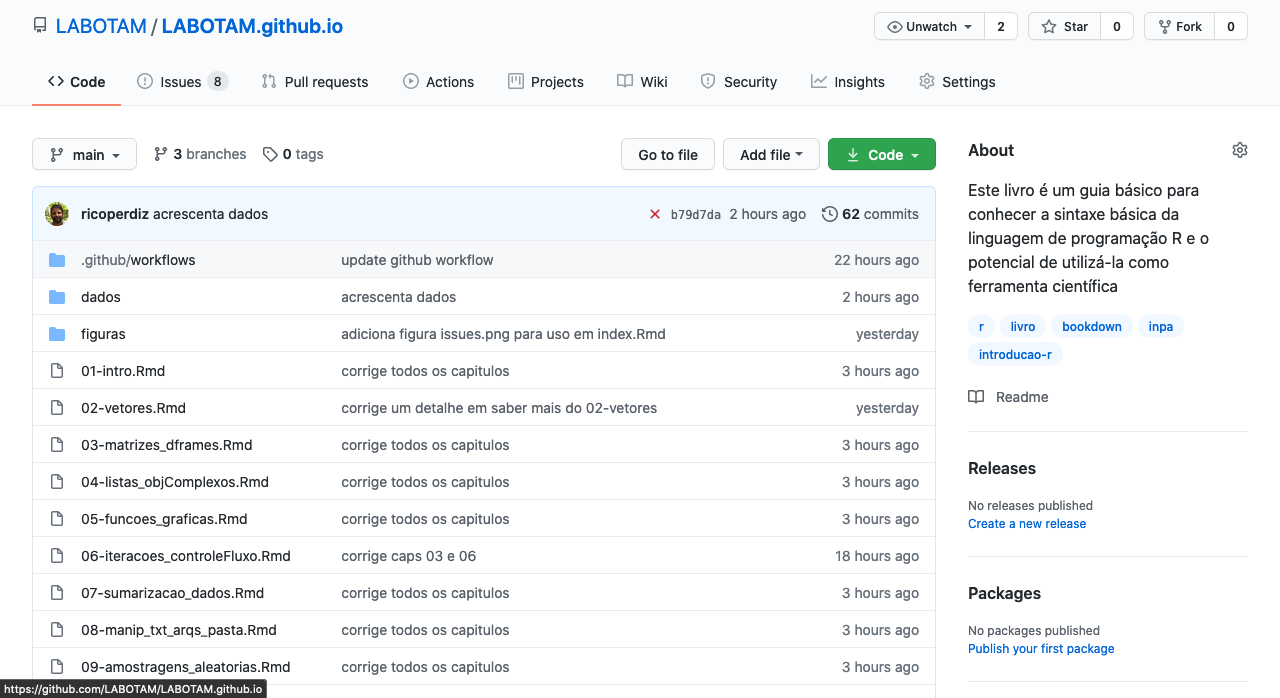
\includegraphics[width=0.8\linewidth]{figuras/repo} \caption{Imagem inicial do repositório hospedado no GitHub contendo o código fonte deste livro.}\label{fig:repo}
\end{figure}

Busque um botão de cor \textbf{verde} chamado \emph{Code} (Fig. \ref{fig:baixa-repo}).
Clique neste botão e aparecerão algumas opções.
Clique no botão \textbf{Download Zip}, destacado em vermelho na figura \ref{fig:baixa-repo}, e escolha onde você quer salvar o arquivo.

\begin{figure}
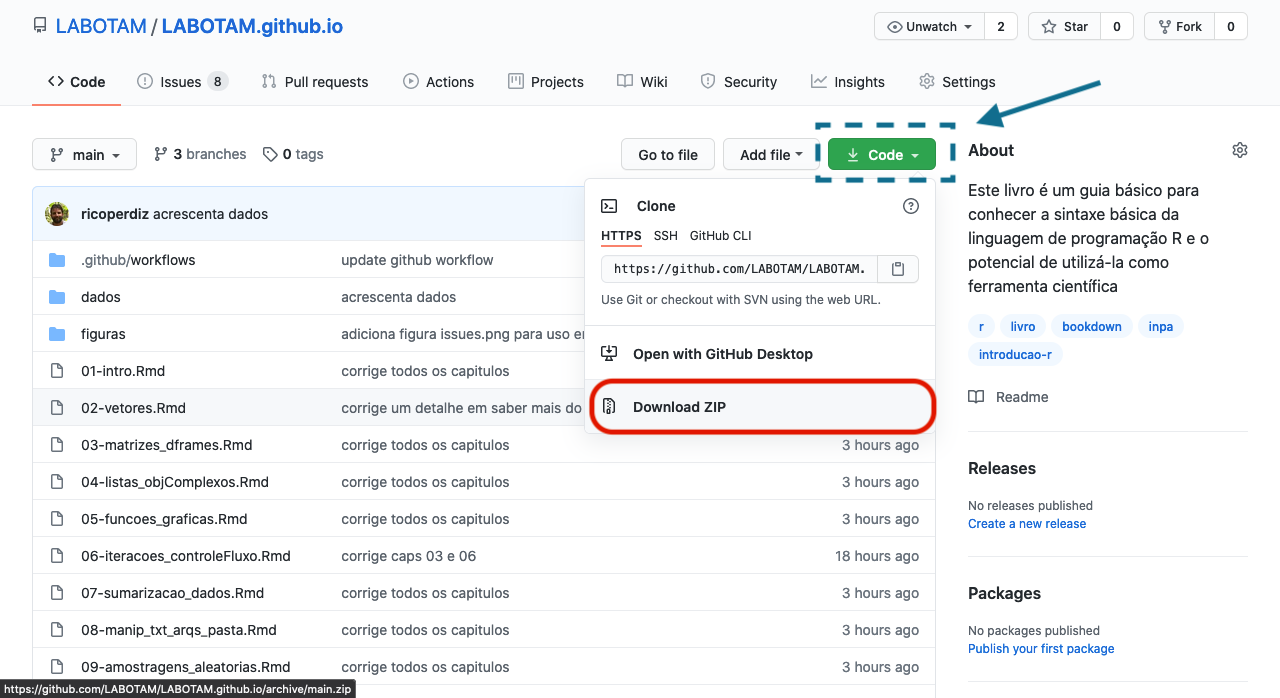
\includegraphics[width=0.6\linewidth]{figuras/baixa_repo} \caption{Destaque do botão "Code" (retângulo "azul" pontilhado circundando o botão, com uma seta "azul" apontando para o mesmo botão) presente na página inicial do repositório hospedado no GitHub contendo o código fonte deste livro. Há um outro retângulo de cor "vermelha" destacando a opção `Download Zip.`}\label{fig:baixa-repo}
\end{figure}

Após baixar, descomprima este arquivo \texttt{.zip}, escolha onde você deseja guardar a pasta, e comece a acessar os arquivos.

Os arquivos contendo cada capítulo deste livro são listados abaixo e podem ser encontrados na \href{https://github.com/LABOTAM/IntroR}{página inicial do repositório}:

\begin{verbatim}
## 00-autores.Rmd
## 01-intro.Rmd
## 02-vetores.Rmd
## 03-matrizes_dframes.Rmd
## 04-listas_objComplexos.Rmd
## 05-funcoes_graficas.Rmd
## 06-iteracoes_controleFluxo.Rmd
## 07-sumarizacao_dados.Rmd
## 08-manip_txt_arqs_pasta.Rmd
## 09-amostragens_aleatorias.Rmd
## 10-extracao_dados.Rmd
## 11-aed_checadados.Rmd
## 12-aed_checaunivar.Rmd
## 13-aed_checabivar.Rmd
## 14-aed_checamultivar.Rmd
## 15-tidyverse.Rmd
## 16-baixa_descomprime.Rmd
## 17-videos_html.Rmd
## 17-videos_pdf.Rmd
## 18-chernoff.Rmd
## 19-referencias.Rmd
\end{verbatim}

Você pode tanto utilizar os arquivos escritos em formato \href{http://www.botanicaamazonica.wiki.br/labotam/doku.php?id=bot89:precurso:rmarkdown:inicio}{Rmarkdown} e executar os códigos em cada célula de código (\textbf{code chunks}) ou usar os scripts contidos na pasta \texttt{codigo}, que nada mais são do que os capítulos do livro convertidos para um script de R, isto é, em formato \texttt{.R}.
Nesses scripts, todos os pedaços de texto, incluindo cabeçalhos e comentários estão precedidos de \texttt{\#\textquotesingle{}}; o que for código aparecerá sem \texttt{\#\textquotesingle{}} precedentes.
Clique no nome dos scripts abaixo para levá-lo direto ao arquivo dentro do repositório.

\begin{itemize}
\tightlist
\item
  \href{https://github.com/LABOTAM/IntroR/tree/main/codigo/00-autores.R}{00-autores.R}
\item
  \href{https://github.com/LABOTAM/IntroR/tree/main/codigo/01-intro.R}{01-intro.R}
\item
  \href{https://github.com/LABOTAM/IntroR/tree/main/codigo/02-vetores.R}{02-vetores.R}
\item
  \href{https://github.com/LABOTAM/IntroR/tree/main/codigo/03-matrizes_dframes.R}{03-matrizes\_dframes.R}
\item
  \href{https://github.com/LABOTAM/IntroR/tree/main/codigo/04-listas_objComplexos.R}{04-listas\_objComplexos.R}
\item
  \href{https://github.com/LABOTAM/IntroR/tree/main/codigo/05-funcoes_graficas.R}{05-funcoes\_graficas.R}
\item
  \href{https://github.com/LABOTAM/IntroR/tree/main/codigo/06-iteracoes_controleFluxo.R}{06-iteracoes\_controleFluxo.R}
\item
  \href{https://github.com/LABOTAM/IntroR/tree/main/codigo/07-sumarizacao_dados.R}{07-sumarizacao\_dados.R}
\item
  \href{https://github.com/LABOTAM/IntroR/tree/main/codigo/08-manip_txt_arqs_pasta.R}{08-manip\_txt\_arqs\_pasta.R}
\item
  \href{https://github.com/LABOTAM/IntroR/tree/main/codigo/09-amostragens_aleatorias.R}{09-amostragens\_aleatorias.R}
\item
  \href{https://github.com/LABOTAM/IntroR/tree/main/codigo/10-extracao_dados.R}{10-extracao\_dados.R}
\item
  \href{https://github.com/LABOTAM/IntroR/tree/main/codigo/11-aed_checadados.R}{11-aed\_checadados.R}
\item
  \href{https://github.com/LABOTAM/IntroR/tree/main/codigo/12-aed_checaunivar.R}{12-aed\_checaunivar.R}
\item
  \href{https://github.com/LABOTAM/IntroR/tree/main/codigo/13-aed_checabivar.R}{13-aed\_checabivar.R}
\item
  \href{https://github.com/LABOTAM/IntroR/tree/main/codigo/14-aed_checamultivar.R}{14-aed\_checamultivar.R}
\item
  \href{https://github.com/LABOTAM/IntroR/tree/main/codigo/15-tidyverse.R}{15-tidyverse.R}
\item
  \href{https://github.com/LABOTAM/IntroR/tree/main/codigo/16-baixa_descomprime.R}{16-baixa\_descomprime.R}
\item
  \href{https://github.com/LABOTAM/IntroR/tree/main/codigo/17-videos_html.R}{17-videos\_html.R}
\item
  \href{https://github.com/LABOTAM/IntroR/tree/main/codigo/17-videos_pdf.R}{17-videos\_pdf.R}
\item
  \href{https://github.com/LABOTAM/IntroR/tree/main/codigo/18-chernoff.R}{18-chernoff.R}
\item
  \href{https://github.com/LABOTAM/IntroR/tree/main/codigo/19-referencias.R}{19-referencias.R}
\end{itemize}

\section*{Caso você não possua um computador}\label{caso-vocuxea-nuxe3o-possua-um-computador}


O Google oferece um serviço chamado \href{https://research.google.com/colaboratory/faq.html}{Google Colab} que pode ser utilizado em computadores, em celulares modernos com acesso à internet e possuídores de um navegador, e em tablets.

Em breve, apresentaremos aqui um endereço contendo todo o conteúdo deste livro já convertido para o formato de um Jupyter Notebook, que é o modelo de arquivo utilizado pelo Google Colab.

\section*{O que é o R e por qual razão você deve se preocupar em programar}\label{o-que-uxe9-o-r-e-por-qual-razuxe3o-vocuxea-deve-se-preocupar-em-programar}


\subsection*{O R em poucas palavras}\label{o-r-em-poucas-palavras}


\begin{quote}
\emph{O R é um software livre e gratuito de desenvolvimento coletivo e é muito útil para quem trabalha com ciências e precisa manipular e analisar dados, gerar gráficos e publicações dinâmicas. Tem uma comunidade enorme de usuários e colaboradores e está disponível gratuitamente em diversos repositórios espalhados pelo mundo} (\url{https://cran.r-project.org/}).
\end{quote}

\begin{quote}
\emph{O R foi criado para permitir a melhor e mais ampla exploração de dados possível, (\ldots) mas sempre explicando a natureza dos métodos utilizados, num formato aberto (livre) e compreensível} \citep{Chambers2008}.
\end{quote}

\begin{quote}
\emph{O R é uma linguagem de programação; você conversa com o R através de um código}.
\end{quote}

\begin{quote}
Por ser uma linguagem de programação, \textbf{no R você pode fazer tudo}. A pergunta não é sobre \textbf{SE} o R faz alguma coisa, mas \textbf{COMO} fazer no R alguma coisa. E há várias maneiras de fazer a mesma coisa no R. É fundamental aprender a falar R, pois sabendo falar você pode dizer do seu jeito.
\end{quote}

\begin{quote}
\emph{Todo estudante de ciências deveria aprender a programar, porque programar lhe ensina a pensar} (Steve Jobs). Usar o R é a melhor forma de aprender estatística porque você precisa de fato entender o que está fazendo ao escrever um código.
\end{quote}

\begin{quote}
\textbf{Aprender a programar é como aprender um novo idioma}; aprendendo o R fica mais fácil aprender outras linguagens de programação e lhe ajuda a aprender inglês, e o inglês lhe facilita falar R.
\end{quote}

\begin{quote}
\textbf{O R é uma fantástica ferramenta para fazer gráficos}; veja exemplos em \url{http://www.r-graph-gallery.com}.
\end{quote}

\begin{quote}
Com o desenvolvimento da linguagem na última década, você pode gerar aplicativos (\href{https://shiny.rstudio.com/}{Shiny}) e relatório dinâmicos usando \href{http://www.botanicaamazonica.wiki.br/labotam/doku.php?id=bot89:precurso:rmarkdown:inicio}{Rmarkdown}, facilitando a formatação gráfica e a reprodutibilidade dos seus artigos, relatórios e projetos científicos.
\end{quote}

\subsection*{Por que programar?}\label{por-que-programar}


\begin{quote}
A maioria dos programas de computador não é muito boa. O código no seu laptop, televisor, telefone, carro é geralmente mal documentado, inconsistente e pouco testado. Por que isso importa para a ciência? Porque transformar dados brutos (\texttt{raw\ data}) em artigos científicos geralmente requer um pouco de programação, o que significa que a maioria dos cientistas escreve software (Nick Barnes, 2010, \href{http://www.nature.com/news/2010/101013/full/467753a.html}{Publish your computer code}, Nature News).
\end{quote}

\begin{quote}
\textbf{É tentador tratar todas as coisas como se fossem pregos, se a única ferramenta que você tem é um martelo} (Abraham Maslow, 1996, \href{https://en.wikipedia.org/wiki/Law_of_the_instrument}{Lei do Instrumento})! Liberte-se da camisa de força dos softwares de estatística que limitam as análises que você pode fazer e como pode fazer.
\end{quote}

\begin{quote}
\emph{Um dos objetivos da análise estatística é o de destilar um conjunto longo e complicado de dados em um número pequeno de estatísticas descritivas que façam sentido. Muitos dos pacotes estatísticos de computadores modernos, no entanto, fazem exatamente o oposto disso. Eles produzem automaticamente um número excessivo de resultados que termina sendo aceito sem crítica; pode levar à super interpretação dos dados; e incentiva o mal hábito de \textbf{jogar dados e cuspir resultados} (data trawling). O R, por outro lado, não lhe diz nada a não ser aquilo que você peça explicitamente} \citep{Crawley2007}.
\end{quote}

\begin{quote}
(\ldots) aprender a programar é importante porque desenvolve habilidades analíticas e de resolução de problemas. É uma atividade criativa, um meio de expressar idéias abstratas. Assim, programar é divertido e é muito mais do que uma habilidade profissional. Ao projetar programas, aprendemos muitas habilidades que são importantes para todas as profissões. Essas habilidades podem ser resumidas como: (1) Leitura crítica, (2) Pensamento analítico, (3) Síntese criativa (\href{http://programmingstage.blogspot.com.br/2012/05/why-programming-is-important.html}{Why programming is important}).
\end{quote}

\begin{quote}
\emph{Uma das coisas mais importantes que você (como cientista) pode fazer é dedicar um tempo para aprender uma linguagem de programação de verdade. Aprender a programar é como aprender outro idioma: exige tempo e treinamento, e não há resultados práticos imediatos. Mas se você supera essa primeira subida íngreme da curva de aprendizado, os ganhos como cientista são enormes. Programar não vai apenas livrar você da camisa de força dos pacotes estatísticos, mas também irá aguçar suas habilidades analíticas e ampliar os horizontes de modelagem (..) e estatística} \citep{Gotelli2013}.
\end{quote}

\begin{figure}
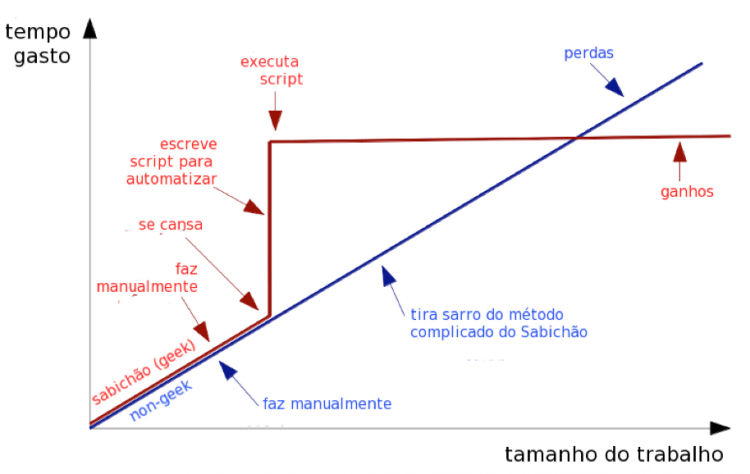
\includegraphics[width=1.01\linewidth]{figuras/aprendizadogeekvsnongeek} \caption{Curvas de aprendizagem do aluno Sabichão (Geek) e de um aluno que tem medo de código (non-geek).}\label{fig:unnamed-chunk-5}
\end{figure}

\section*{Análise exploratória de dados (AED)}\label{anuxe1lise-exploratuxf3ria-de-dados-aed}


\subsection*{O que é AED e por que fazer AED?}\label{o-que-uxe9-aed-e-por-que-fazer-aed}


\begin{quote}
Em estatística, análise exploratória de dados (AED) é uma abordagem para analisar conjuntos de dados visando resumir as suas principais características, particularmente com métodos gráficos e visuais.
Um modelo estatístico pode ou não ser usado, mas AED objetiva principalmente ver o que os dados podem nos dizer para além da modelagem ou de testes de hipóteses. A AED foi promovida por \href{https://en.wikipedia.org/wiki/John_Tukey}{John Tukey} para incentivar estatísticos a explorar dados e, eventualmente, formular novas hipóteses que possam levar à nova coleta de dados e a experimentos.
AED é diferente de análise de dados inicial (AID), que foca mais estreitamente na verificação de suposições necessárias aos modelos de testes de hipóteses, manipulação de valores ausentes e transformações de variáveis, conforme necessário.
AED abrange AID (Texto traduzido da \href{https://en.wikipedia.org/wiki/Exploratory_data_analysis}{WikiPedia}).
\end{quote}

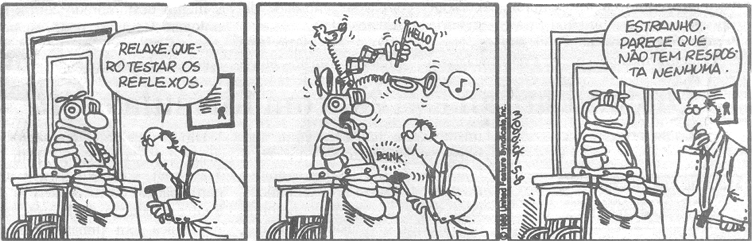
\includegraphics[width=1\linewidth]{figuras/aed}

\begin{quote}
Muitas vezes esquecemos como funciona a ciência e a engenharia. Idéias vêm mais frequentemente de exploração anterior do que de descargas atmosféricas. (\ldots) \textbf{Encontrar a pergunta é muitas vezes mais importante do que encontrar a resposta}. Análise exploratória de dados é uma atitude, uma flexibilidade que depende de visualização gráfica, não é um conjunto de técnicas \citep{Tukey1980}.
\end{quote}

Em sistemática e taxonomia, uma ciência histórica, a análise exploratória é fundamental, pois é através dela que podemos postular boas hipóteses e usar teste de hipóteses para confirmá-las.

\begin{quote}
Aplicar a análise exploratória de dados para criar hipóteses e então usar os mesmos dados para testar essas hipóteses deve ser evitado.
Se alguém tem conhecimento \emph{a priori} limitado, então uma abordagem válida é criar dois conjuntos de dados: aplicar exploração de dados sobre o primeiro conjunto para criar hipóteses e usar o segundo conjunto de dados para testar essas hipóteses .
Tal processo, no entanto, só é prático para conjuntos de dados grandes.
Independentemente da situação específica, o uso constante e a estruturação de relatórios transparentes de exploração sistemática de dados melhorariam a qualidade da pesquisa ecológica e de quaisquer recomendações que ela produziria \citep{Zuuretal2010}.
\end{quote}

A análise exploratória não é \emph{dragagem} de dados! Assume-se que o pesquisador formulou hipóteses biológicas plausíveis \emph{a priori} amparadas pela teoria.

\subsection*{Objetivos da AED}\label{objetivos-da-aed}


\begin{itemize}
\tightlist
\item
  Controlar a qualidade dos dados;
\item
  Sugerir hipóteses para os padrões observados (novos estudos);
\item
  Apoiar a escolha dos procedimentos estatísticos de testes de hipótese;
\item
  Avaliar se os dados atendem às premissas dos procedimentos estatísticos escolhidos.
\end{itemize}

\subsection*{Para ler}\label{para-ler}


Dois artigos que você deveria ler: \citet{Tukey1980} e \citet{Zuuretal2010}.

\section*{\texorpdfstring{Exercícios no \textbf{notaR}}{Exercícios no notaR}}\label{exercuxedcios-no-notar}


Ao fim de alguns capítulos, disponibilizaremos em seções chamadas \textbf{Exercícios} uma lista de endereços ligados ao \href{http://www.lage.ib.usp.br/notar/index.php}{notaR}, um sistema criado para auxiliar no aprendizado da linguagem R desenvolvido pelo laboratório de Ecologia Teórica da Universidade de São Paulo \citep{Chalometal2012}.

\subsection*{\texorpdfstring{Conhecendo o \textbf{notaR}}{Conhecendo o notaR}}\label{conhecendo-o-notar}


Os exercícios do notaR obrigam o usuário a construir um script de R a partir de um enunciado, acabando por fugir do tradicional \textbf{copia-cola} de tutoriais de R.
Muitos exercícios no sistema não obrigam o usuário a estar autenticado (estar logado usando login e senha) no sistema para poder fazê-los.
Leia com atenção o enunciado de cada exercício antes de iniciar a construir o seu script.

Uma lista de todos os exercícios \textbf{notaR} incluídos neste livro está relacionada abaixo:

\begin{itemize}
\tightlist
\item
  Resolva o exercício \href{http://notar.ib.usp.br/exercicio/29}{101.01 Bem vindo ao notaR}.
\item
  Resolva o exercício \href{http://notar.ib.usp.br/exercicio/15}{101.05 Remoção Com Critério}.
\item
  Resolva o exercício \href{http://notar.ib.usp.br/exercicio/19}{102.04 Biomassa de Árvores}.
\item
  Resolva o exercício \href{http://notar.ib.usp.br/exercicio/12}{102.02 Sequências}.
\item
  Resolva o exercício \href{http://notar.ib.usp.br/exercicio/4}{102.03 Conta de Luz}.
\item
  Resolva o exercício \href{http://notar.ib.usp.br/exercicio/17}{102.01 Área Basal}.
\item
  Resolva o exercício \href{http://notar.ib.usp.br/exercicio/5}{102.05 Variância na Unha}.
\item
  Resolva o exercício \href{http://notar.ib.usp.br/exercicio/18}{101.03 Objetos de Data}.
\item
  Resolva o exercício \href{http://notar.ib.usp.br/exercicio/23}{103.01 Distância entre cidades}.
\item
  Resolva o exercício \href{http://notar.ib.usp.br/exercicio/2}{103.02 Criação de um data frame}.
\item
  Resolva o exercício \href{http://notar.ib.usp.br/exercicio/13}{103.03 Criando uma Matriz}.
\item
  Resolva o exercício \href{http://notar.ib.usp.br/exercicio/66}{302.02 Histogramas (frequência)}.
\item
  Resolva o exercício \href{http://notar.ib.usp.br/exercicio/71}{302.07 Gráficos com trechos selecionados do data.frame/matriz}.
\item
  Resolva o exercício \href{http://notar.ib.usp.br/exercicio/67}{302.04 Box-plots}.
\item
  Resolva o exercício \href{http://notar.ib.usp.br/exercicio/69}{302.05 Gráficos de dispersão}.
\item
  Resolva o exercício \href{http://notar.ib.usp.br/exercicio/70}{302.06 Matriz de dispersão}.
\item
  Resolva o exercício \href{http://notar.ib.usp.br/exercicio/75}{Editando parâmetros gráficos}.
\item
  Resolva o exercício \href{http://notar.ib.usp.br/exercicio/14}{104.01 Sintetizando dados}.
\item
  Resolva o exercício \href{http://notar.ib.usp.br/exercicio/21}{103.05 Classes de Objetos}.
\item
  Resolva o exercício \href{http://notar.ib.usp.br/exercicio/22}{103.04 Lendo e salvando seus dados}.
\item
  Resolva o exercício \href{http://notar.ib.usp.br/exercicio/34}{103.7 Cara ou coroa}.
\item
  Resolva o exercício \href{http://notar.ib.usp.br/exercicio/37}{103.9 Lembrando matrizes e listas}.
\end{itemize}

\section*{Referências úteis}\label{referuxeancias-uxfateis}


Listamos abaixo algumas referências importantes para complementar o seu estudo:

\begin{itemize}
\tightlist
\item
  \href{http://ecologia.ib.usp.br/bie5782/doku.php?id=bie5782:02_tutoriais:tutorial4:start}{Apostila USP-BIE-5782}.
\item
  \href{https://cran.r-project.org/doc/manuals/R-intro.html}{Introdução ao R no site do R}.
\item
  \href{https://6e938257-ec28-4b42-9917-4ed33b2f1d0b.filesusr.com/ugd/e086b2_0d0de99bbb204ca68e079b4ae11b87d6.docx?dn=A_apostila_de_introdu\%C3\%A7\%C3\%A3o_ao_R_vers\%C3\%A3o_6.3.1_2018.docx}{Introdução ao uso do programa R de Victor Landeiro e Fabricio Baccaro}.
\item
  \href{http://www.botanicaamazonica.wiki.br/labotam/doku.php?id=bot89:precurso:rmarkdown:inicio}{Relatórios dinâmicos com R Markdown}.
\end{itemize}

\chapter*{Sobre os autores}\label{sobre-os-autores}


Alberto é doutor em Ecologia, Evolução e Sistemática, com uma ênfase em Evolução pela Universidade do Missouri, Saint Louis (University of Missouri Saint Louis).
É cientista do Instituto Nacional de Pesquisas da Amazônia (INPA) desde o ano de 2009.
Ministra anualmente disciplinas ligadas ao Programa de pós-graduação em Ciências Biológicas do INPA, como \textbf{Preparação de dados para análises Estáticas - Introdução ao uso de linguagem R (BOT-89)}, \textbf{Delineamento Experimental e Amostral (BOT-90)}, e \textbf{Teoria e Prática de Sistemática Filogenética (BOT-99)}.
É colíder do grupo de pesquisa \href{http://dgp.cnpq.br/dgp/espelhogrupo/38425}{Ecologia e Evolução de Plantas da Amazônia} do Conselho Nacional de Desenvolvimento Científico e Tecnológico (CNPq).

\href{https://www.ricardoperdiz.com}{Ricardo} é doutor em Ciências Biológicas (Botânica) pelo INPA.
Seus principais interesses são estar e se divertir com a família, trabalhar na floresta coletando e admirando a beleza da Natureza, trabalhar no herbário e laboratório, e também adora se divertir na frente do computador analisando dados e escrevendo.
Ama correr e pedalar, e também se divertir e aprender com sua filha.

\mainmatter

\part{Parte I}\label{part-parte-i}

Um passo a passo para conhecer a sintaxe básica da linguagem de programação e o potencial de usar o R como ferramenta científica.

\chapter{Conceitos introdutórios}\label{intro}

Recomendamos que o usuário siga a ordem dos capítulos, especialmente se é a primeira vez que o mesmo está lidando com o R.
Use o R via RStudio, é mais simples.
Busque executar cada script linha por linha, procurando entender o que cada linha faz e o que cada comando representa.
E para cada função nova, busque a \hyperref[help]{ajuda do R}, leia o que significam cada um dos argumentos.
Altere os argumentos das funções e veja o que acontece.
Explore!

\section{Console e scripts}\label{console-e-scripts}

As figuras abaixo mostram imagens relativamente similares ao que os usuários do R padrão (Figura \ref{fig:pad-r}) e RStudio (Figura \ref{fig:studio-r}) verão ao iniciarem esses programas.

\begin{figure}
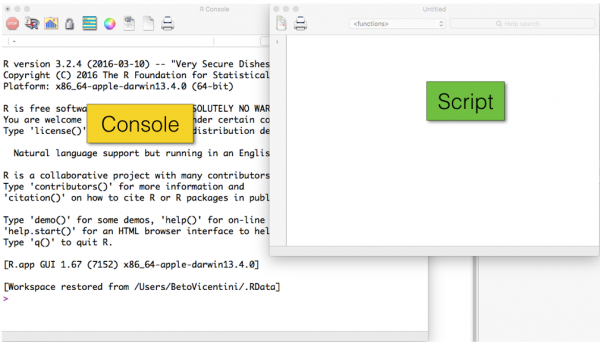
\includegraphics[width=0.33\linewidth]{figuras/r_padrao} \caption{ Imagem de uma sessão do R para Mac OSX com um janela de script aberta além do console.}\label{fig:pad-r}
\end{figure}

Ao abrirem o R ou o RStudio você terão basicamente duas janelas principais:

\begin{itemize}
\item
  \textbf{Console} - corresponde à interface que interpreta o código da linguagem. Os códigos digitados aqui serão interpretados pelo R (Texto destacado em \textbf{verde} nas figuras \ref{fig:pad-r}, \ref{fig:studio-r});
\item
  \textbf{Script} - digitar um código curto no console é simples, mas quando o código é longo, é importante guardá-lo em algum lugar para executá-lo em qualquer momento. Para isso utilizamos scripts, que são arquivos de textos simples que podem ser salvo (extensão \texttt{.R}) numa pasta no seu computador e reutilizado (Texto destacado em \textbf{amarelo} nas figuras \ref{fig:pad-r}, \ref{fig:studio-r}). Como um arquivo \texttt{.R} é um texto simples, ele é editável por qualquer editor de texto, como o Bloco de Notas ou \href{https://notepad-plus-plus.org/}{Notepad++} para usuários Windows, \href{https://www.barebones.com/products/textwrangler/}{TextWrangler} ou \href{https://www.barebones.com/products/textwrangler/}{BBEdit} para usuários macOS, ou \href{https://help.gnome.org/users/gedit/stable/index.html.pt_BR}{gedit} para usuários Linux. O editor de scripts do RStudio é excelente.
\end{itemize}

\begin{figure}
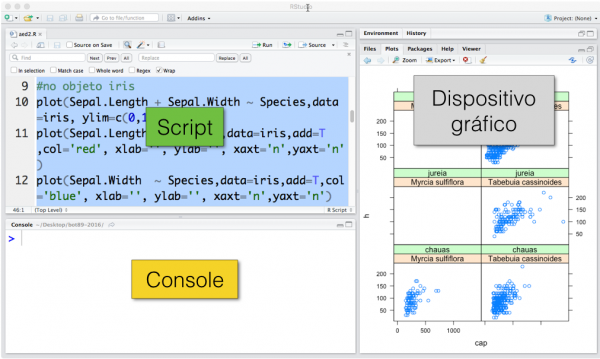
\includegraphics[width=1\linewidth]{figuras/rstudio} \caption{ Imagem de uma sessão do RStudio com três painéis abertos.}\label{fig:studio-r}
\end{figure}

\section{Linguagem objeto-orientada}\label{linguagem-objeto-orientada}

A chave para entender o R é que trata-se de uma linguagem.
Uma linguagem para manipular objetos \citep{VenablesRipley2002}.
Um objeto é identificado por uma palavra e veremos ao longo do curso que existem vários tipos de objetos.
Este é o conceito mais importante para entender o R.

Para começar, digite algumas coisas no Console do seu R ou RStudio.
Por exemplo, digite uma fórmula matemática simples no console e o execute:

\begin{Shaded}
\begin{Highlighting}[]
\DecValTok{3} \SpecialCharTok{+} \DecValTok{5} \SpecialCharTok{+} \DecValTok{10}
\end{Highlighting}
\end{Shaded}

\begin{verbatim}
## [1] 18
\end{verbatim}

O console retornou 18, isto é, o R funcionou como uma calculadora.
Portanto, números são interpretados como números pelo console.

Agora vamos criar um objeto simples chamado \texttt{objnum} e atribuir texto a ele:

\begin{Shaded}
\begin{Highlighting}[]
\NormalTok{objum }\OtherTok{\textless{}{-}} \StringTok{"vou colocar um texto dentro do meu primeiro objeto"} \CommentTok{\# enter}
\NormalTok{objum }\CommentTok{\# enter}
\end{Highlighting}
\end{Shaded}

\begin{verbatim}
## [1] "vou colocar um texto dentro do meu primeiro objeto"
\end{verbatim}

Vejam que \texttt{objum} é o nome do meu primeiro objeto, e tem como conteúdo o texto que nós atribuímos a ele.
Nós poderíamos ter chamado \texttt{objum} de qualquer coisa (sem espaços em branco):

\begin{Shaded}
\begin{Highlighting}[]
\NormalTok{banana }\OtherTok{\textless{}{-}} \StringTok{"vou colocar um texto dentro do meu primeiro objeto"}
\NormalTok{banana}
\end{Highlighting}
\end{Shaded}

\begin{verbatim}
## [1] "vou colocar um texto dentro do meu primeiro objeto"
\end{verbatim}

\begin{Shaded}
\begin{Highlighting}[]
\CommentTok{\# mesma coisa né?}
\end{Highlighting}
\end{Shaded}

Um objeto também pode virar outro objeto. Vejamos abaixo:

\begin{Shaded}
\begin{Highlighting}[]
\NormalTok{objdois }\OtherTok{\textless{}{-}}\NormalTok{ objum}
\NormalTok{objdois }\CommentTok{\# pegou o conteúdo que eu coloquei em objum}
\end{Highlighting}
\end{Shaded}

\begin{verbatim}
## [1] "vou colocar um texto dentro do meu primeiro objeto"
\end{verbatim}

Podemos guardar resultados de contas em um objeto:

\begin{Shaded}
\begin{Highlighting}[]
\NormalTok{objtres }\OtherTok{\textless{}{-}} \DecValTok{3} \SpecialCharTok{+} \DecValTok{5} \SpecialCharTok{+} \DecValTok{10}
\NormalTok{objtres}
\end{Highlighting}
\end{Shaded}

\begin{verbatim}
## [1] 18
\end{verbatim}

Note que o código exposto acima é geralmente o que está contido em um \href{https://pt.wikipedia.org/wiki/Linguagem_de_script}{script}, ou seja, a sequência de códigos que você escreveu e que o R interpretará para realizar o que foi dito.
Se você copiar e colar o trecho (ou os trechos) de código acima em um arquivo \texttt{.R}, você poderá executá-los tantas vezes quanto quiser.
Copie então todos os trechos de código expostos até então para a janela do script e salve-o como \texttt{script01.R} em alguma pasta no seu computador.

Note também que dependendo do está incluso no script, o código apresenta cores diferentes para comentários, objetos, e símbolos de atribuição.
Isso ajuda a entender os elementos da sintaxe (vocabulário e gramática do R).
IDE's também mostram isso de forma colorida.

Note também que, à direita do símbolo \texttt{\#}, o texto no código acima fica cinza.
Este símbolo indica ao R que todo texto começando no \texttt{\#} deve ser interpretado como texto apenas, e não como código.
Comentar códigos é uma prática que deve ser tornar rotineira a fim de facilitar o entendimento de cada script.

Se você já está escrevendo um script num arquivo e não no console, selecione todo o texto na sua janela de script e digite \texttt{Control+R} (Windows), ou \texttt{Command+Enter} (Mac).
O conteúdo do script será executado no Console.
Note que o símbolo \texttt{\#} não é interpretado pelo console.

O R vem com vários scripts prontos, que são funções que executam alguma coisa.
Esses scripts são objetos de classe \textbf{função}, pois eles contêm um conjunto de códigos que utilizam parâmetros para executar um conjunto de passos.
Parâmetros são objetos que a função utiliza segundo as suas especificações.
Por exemplo, vamos listar os objetos criados no passo anterior:

\begin{Shaded}
\begin{Highlighting}[]
\CommentTok{\# digite}
\FunctionTok{ls}\NormalTok{() }\CommentTok{\# note os parênteses (); a função ls() lista os objetos criados por você: [1] "banana"  "objdois" "objtres" "objum"}

\CommentTok{\# adicione um parâmetro à função, especificando o que você quer listar, apenas aqueles que contém no nome o padrão "obj"}
\FunctionTok{ls}\NormalTok{(}\AttributeTok{pattern =} \StringTok{"obj"}\NormalTok{) }\CommentTok{\# [1] "objdois" "objtres" "objum"}

\CommentTok{\# agora veja o que a função ls é}
\NormalTok{ls }\CommentTok{\# note que não digitei os parênteses e ao digitar isso verei o script que está dentro da função ls que começa assim: function (name, pos = {-}1L, envir = as.environment(pos), all.names = FALSE, pattern, sorted = TRUE)  \{ ....}
\CommentTok{\# note que os argumentos da função são os objetos que vão dentro do () da função e são utilizados pela função para executar alguma coisa, neste caso, lista objetos. Experimente mudando parâmetros:}
\FunctionTok{ls}\NormalTok{(}\AttributeTok{sorted =} \ConstantTok{FALSE}\NormalTok{) }\CommentTok{\# ele mostra os objetos na ordem que foram criados}
\end{Highlighting}
\end{Shaded}

\section{R-base e pacotes}\label{base-pacotes}

Como vimos acima, um script do tipo função é um objeto que executa um conjunto de comandos e recebe argumentos que modificam o que o script realiza. Existem dois tipos de funções:

\begin{itemize}
\item
  Funções do pacote \texttt{base} - funções que vêm junto com o R quando você faz o download do programa, como por exemplo as funções \texttt{length()}, \texttt{order()}, \texttt{sort()}, \texttt{sum()}, \texttt{mean()} etc;
\item
  Funções de pacotes externos - pacotes (\texttt{packages} em inglês) são funções criadas por colaboradores e organizadas em pacotes que você pode baixar dos repositórios do R.
\end{itemize}

As funções do pacote \texttt{base} vêm junto com o programa e você não precisa se preocupar com isso.
Pacotes, por outro lado, devem ser instalados pelo usuário conforme a necessidade.
Por exemplo, para trabalhar com dados filogenéticos, você pode necessitar do pacote \href{https://cran.r-project.org/web/packages/ape/index.html}{ape} \citep{R-ape}, que já tem várias funções preparadas para análises filogenéticas.
Se você necessitar deste pacote, por exemplo, basta executar o seguinte comando no console do R:

\begin{Shaded}
\begin{Highlighting}[]
\FunctionTok{install.packages}\NormalTok{(}\StringTok{"ape"}\NormalTok{)}
\end{Highlighting}
\end{Shaded}

Para trabalhar com pacotes você primeiro precisa definir um repositório, ou seja, um servidor, de vários disponíveis (espelhos do repositório oficial), de onde o R buscará o pacote desejado.
Pode-se também o menu do R ou do RStudio para instalar pacotes e definir um repositório padrão para sua instalação.

Como tudo no R, você pode executar comandos que estão no menu usando funções.
Por exemplo, ao invés de usarmos o menu do R para definir um repositório e instalar um pacote, vamos executar estas ações por meio de um script:

\begin{Shaded}
\begin{Highlighting}[]
\CommentTok{\# isso pode não funcionar se estiver no INPA por causa do Proxy.}
\FunctionTok{chooseCRANmirror}\NormalTok{() }\CommentTok{\# seleciona repositório}
\FunctionTok{install.packages}\NormalTok{(}\StringTok{"ape"}\NormalTok{, }\AttributeTok{dependencies =} \ConstantTok{TRUE}\NormalTok{) }\CommentTok{\# instala o pacote Ape}
\end{Highlighting}
\end{Shaded}

\section{Ajuda no R}\label{help}

Toda função no R, oriunda tanto do pacote base ou dos pacotes extras, possui um pedaço de texto chamado de ``ajuda'' e que possui uma instrução sobre a utilização da mesma.
Para obter esta instrução, é muito fácil.
Basta executar uma das seguintes opções:

\begin{Shaded}
\begin{Highlighting}[]
\CommentTok{\# como exemplo vamos usar a função ls()}
\NormalTok{?ls }\CommentTok{\# ou seja o comando é ?+"nome da função"}
\CommentTok{\# ou então}
\FunctionTok{help}\NormalTok{(}\AttributeTok{topic =} \StringTok{"ls"}\NormalTok{) }\CommentTok{\# nome da função como argumento da topic da função help}
\end{Highlighting}
\end{Shaded}

Ao digitar uma das opções acima, o R vai abrir uma janela (no RStudio, vai colocar esse resultado num dos painéis) contendo a página com a explicação da função:

\begin{Shaded}
\begin{Highlighting}[]
\NormalTok{?ls}
\end{Highlighting}
\end{Shaded}

\begin{verbatim}
## List Objects
## 
## Description:
## 
##      'ls' and 'objects' return a vector of character strings giving the
##      names of the objects in the specified environment.  When invoked
##      with no argument at the top level prompt, 'ls' shows what data
##      sets and functions a user has defined.  When invoked with no
##      argument inside a function, 'ls' returns the names of the
##      function's local variables: this is useful in conjunction with
##      'browser'.
## 
## Usage:
## 
##      ls(name, pos = -1L, envir = as.environment(pos),
##         all.names = FALSE, pattern, sorted = TRUE)
##      objects(name, pos= -1L, envir = as.environment(pos),
##              all.names = FALSE, pattern, sorted = TRUE)
##      
## Arguments:
## 
##     name: which environment to use in listing the available objects.
##           Defaults to the _current_ environment.  Although called
##           'name' for back compatibility, in fact this argument can
##           specify the environment in any form; see the 'Details'
##           section.
## 
##      pos: an alternative argument to 'name' for specifying the
##           environment as a position in the search list.  Mostly there
##           for back compatibility.
## 
##    envir: an alternative argument to 'name' for specifying the
##           environment.  Mostly there for back compatibility.
## 
## all.names: a logical value.  If 'TRUE', all object names are returned.
##           If 'FALSE', names which begin with a '.' are omitted.
## 
##  pattern: an optional regular expression.  Only names matching
##           'pattern' are returned.  'glob2rx' can be used to convert
##           wildcard patterns to regular expressions.
## 
##   sorted: logical indicating if the resulting 'character' should be
##           sorted alphabetically.  Note that this is part of 'ls()' may
##           take most of the time.
## 
## Details:
## 
##      The 'name' argument can specify the environment from which object
##      names are taken in one of several forms: as an integer (the
##      position in the 'search' list); as the character string name of an
##      element in the search list; or as an explicit 'environment'
##      (including using 'sys.frame' to access the currently active
##      function calls).  By default, the environment of the call to 'ls'
##      or 'objects' is used. The 'pos' and 'envir' arguments are an
##      alternative way to specify an environment, but are primarily there
##      for back compatibility.
## 
##      Note that the _order_ of strings for 'sorted = TRUE' is locale
##      dependent, see 'Sys.getlocale'.  If 'sorted = FALSE' the order is
##      arbitrary, depending if the environment is hashed, the order of
##      insertion of objects, ....
## 
## References:
## 
##      Becker, R. A., Chambers, J. M. and Wilks, A. R. (1988) _The New S
##      Language_.  Wadsworth & Brooks/Cole.
## 
## See Also:
## 
##      'glob2rx' for converting wildcard patterns to regular expressions.
## 
##      'ls.str' for a long listing based on 'str'.  'apropos' (or 'find')
##      for finding objects in the whole search path; 'grep' for more
##      details on 'regular expressions'; 'class', 'methods', etc., for
##      object-oriented programming.
## 
## Examples:
## 
##      .Ob <- 1
##      ls(pattern = "O")
##      ls(pattern= "O", all.names = TRUE)    # also shows ".[foo]"
##      
##      # shows an empty list because inside myfunc no variables are defined
##      myfunc <- function() {ls()}
##      myfunc()
##      
##      # define a local variable inside myfunc
##      myfunc <- function() {y <- 1; ls()}
##      myfunc()                # shows "y"
\end{verbatim}

Todos esses trechos de ajuda (\texttt{?}) do R têm a mesma estrutura e devem ser acessados constantemente para o bom entendimento do funcionamento das funções e seus argumentos.

\section{Área de trabalho vs.~Pasta de Trabalho}\label{uxe1rea-de-trabalho-vs.-pasta-de-trabalho}

Dois conceitos são fundamentais para trabalhar no R:

\begin{itemize}
\tightlist
\item
  Área de Trabalho (\texttt{environment} no R) - é o local dentro do R onde você coloca os objetos criados durante a execução de scripts. Você pode visualizar/apagar os objetos no Console:
\end{itemize}

\begin{Shaded}
\begin{Highlighting}[]
\FunctionTok{ls}\NormalTok{() }\CommentTok{\# ls= listar {-} já vimos que isso lista os objetos criados por você e que estão na área de trabalho}

\NormalTok{?rm }\CommentTok{\# veja o help desta função}
\FunctionTok{rm}\NormalTok{(objum) }\CommentTok{\# rm = remover {-} esta função apaga objetos da área de trabalho. No exemplo estamos apagando o objeto chamado objum, criado anteriormente}
\FunctionTok{ls}\NormalTok{() }\CommentTok{\# note agora que o objeto não existe mais}

\FunctionTok{rm}\NormalTok{(}\AttributeTok{list =} \FunctionTok{ls}\NormalTok{()) }\CommentTok{\# desse jeito apagamos todos os objetos que criamos anteriormente}
\FunctionTok{ls}\NormalTok{() }\CommentTok{\# note que não sobrou nenhum objeto}
\end{Highlighting}
\end{Shaded}

\begin{itemize}
\tightlist
\item
  Pasta de Trabalho (\texttt{working\ directory}- é o local (pasta) no seu computador que o R usa para salvar arquivos. É o caminho padrão para o R encontrar arquivos de dados, scripts, etc. Você pode trabalhar no R sem definir uma \textbf{Pasta de Trabalho} mas é muito mais simples se você usa este recurso. Experimente a seguinte script:
\end{itemize}

\begin{Shaded}
\begin{Highlighting}[]
\FunctionTok{getwd}\NormalTok{() }\CommentTok{\# o nome desta função é abreviação de "get working directory" ou seja "pega a pasta de trabalho definida". A resposta deste código varia dependendo do seu sistema operacional. Mas a função retorna o caminho completo da pasta de trabalho atual}
\end{Highlighting}
\end{Shaded}

Toda vez que você usar o R, é uma boa prática primeiramente definir a \emph{pasta de trabalho}, que é o local no seu computador onde você guarda os arquivos relacionados ao seu projeto (dados, scripts, resultados etc.).

Você pode definir a \emph{pasta de trabalho} usando o menu do R (\texttt{Arquivo\ ⇒\ Diretório\ de\ Trabalho} no Windows; ou \texttt{Misc\ ⇒\ Muda\ Pasta\ de\ Trabalho} no Mac).
Ou você pode usar uma função:

\begin{Shaded}
\begin{Highlighting}[]
\NormalTok{?setwd }\CommentTok{\# veja o help da função que iremos utilizar}
\NormalTok{minhapasta }\OtherTok{\textless{}{-}} \StringTok{"/Users/BetoVicentini/Desktop/bot89{-}2016"}
\CommentTok{\# se estiver usando windows:}
\CommentTok{\# minhapasta = "c:/Users/BetoVicentini/Documents/bot89{-}2016"}
\CommentTok{\# minhapasta = "c:\textbackslash{}\textbackslash{}/Users\textbackslash{}\textbackslash{}/BetoVicentini\textbackslash{}\textbackslash{}/Documents\textbackslash{}\textbackslash{}/bot89{-}2016"  \#talvez precise usar barras invertidas}

\FunctionTok{setwd}\NormalTok{(}\AttributeTok{dir =}\NormalTok{ minhapasta) }\CommentTok{\# usa a funçao "set working directory" para especificar o diretório (pasta) de trabalho}
\CommentTok{\# note que eu defini dir primeiramente como o objeto "minhapasta" usei esse objeto para especificar o objeto "dir", que é o único argumento da função setwd()}
\end{Highlighting}
\end{Shaded}

Objetos criados no R por você podem ser salvos como um arquivo no seu computador.
Você pode usar o menu do R ou RStudio para isso ou pode usar o comando abaixo:

\begin{Shaded}
\begin{Highlighting}[]
\NormalTok{?save }\CommentTok{\# veja o help desta função que vamos utilizar}
\NormalTok{?save.image }\CommentTok{\# veja o help desta função que vamos utilizar}

\CommentTok{\# se sua área de trabalho estiver vazia}
\FunctionTok{ls}\NormalTok{() }\CommentTok{\# se nao retorna nada porque voce apagou acima}
\CommentTok{\# crie alguns objetos para o exercício}
\NormalTok{objum }\OtherTok{\textless{}{-}} \StringTok{"um objeto de texto qualquer"}
\NormalTok{objum}
\NormalTok{objdois }\OtherTok{\textless{}{-}} \DecValTok{18} \CommentTok{\# um objeto com um número qualquer}
\NormalTok{objdois}
\NormalTok{banana }\OtherTok{\textless{}{-}}\NormalTok{ objum }\CommentTok{\# um objeto idêntico a objum}

\CommentTok{\# pronto, agora mostre todos os objetos na sua AREA DE TRABALHO}
\FunctionTok{ls}\NormalTok{()}

\CommentTok{\# agora salve esse objetos como um arquivo na sua PASTA DE TRABALHO}
\FunctionTok{getwd}\NormalTok{() }\CommentTok{\# veja onde o arquivo será salvo}

\CommentTok{\# se voce quer salvar todos os objetos}
\FunctionTok{save.image}\NormalTok{(}\AttributeTok{file =} \StringTok{"meusObjetos.Rdata"}\NormalTok{)}

\CommentTok{\# se voce quer salvar apenas alguns objetos}
\FunctionTok{save}\NormalTok{(objum, banana, }\AttributeTok{file =} \StringTok{"meusObjetos2.Rdata"}\NormalTok{)}

\CommentTok{\# veja que na sua pasta de trabalho getwd() voce tem esses arquivos}
\FunctionTok{dir}\NormalTok{() }\CommentTok{\# lista arquivos na sua pasta de trabalho (análoga a função ls() que lista objetos)}
\FunctionTok{dir}\NormalTok{(}\AttributeTok{pattern =} \StringTok{"Rdata"}\NormalTok{) }\CommentTok{\# lista apenas arquivos que tem no nome ".Rdata"}

\CommentTok{\# apaga os objetos todos}
\FunctionTok{rm}\NormalTok{(}\AttributeTok{list =} \FunctionTok{ls}\NormalTok{())}
\FunctionTok{ls}\NormalTok{() }\CommentTok{\# note que não tem mais objetos na sua área de trabalho, mas pode resgatar objetos que salvou num arquivo Rdata:}
\FunctionTok{load}\NormalTok{(}\AttributeTok{file =} \StringTok{"meusObjetos2.Rdata"}\NormalTok{) }\CommentTok{\# puxa os objetos neste arquivo que está na sua pasta de trabalho}
\FunctionTok{ls}\NormalTok{() }\CommentTok{\# note que ele puxou os objetos objum e banana que salvamos acima neste arquivo}

\CommentTok{\# puxe o outro arquivo gerado}
\FunctionTok{load}\NormalTok{(}\AttributeTok{file =} \StringTok{"meusObjetos.Rdata"}\NormalTok{) }\CommentTok{\# puxa os objetos neste arquivo que está na sua pasta de trabalho}
\FunctionTok{ls}\NormalTok{() }\CommentTok{\# veja novamente os objetos na sua área de trabalho: Todos os objetos são listados. Se fizer isso e já houver objetos com o mesmo nome na sua área de trabalho, estes serão sobrepostos.}
\end{Highlighting}
\end{Shaded}

Portanto, \emph{Área de Trabalho} e \emph{Pasta de Trabalho} são dois conceitos fundamentais que você precisa entender bem, pois define como e onde você estará salvando informação quando usar o R, tanto em termos de objetos (área de trabalho) como em termos de arquivos (pasta de trabalho).

Se você digita \texttt{q()}, que é a função para sair do R, ele geralmente lhe pergunta se você quer salvar os objetos numa área de trabalho padrão (que o R puxa quando você o inicia):

\begin{Shaded}
\begin{Highlighting}[]
\FunctionTok{q}\NormalTok{() }\CommentTok{\# sai do R}
\CommentTok{\# vai perguntar no Console algo do tipo "Save workspace image to \textasciitilde{}/Desktop/bot89{-}2016/.RData? [y/n/c]:"}
\CommentTok{\# note que o arquivo não tem nome apenas extensão ".RData" e é salvo na pasta de trabalho definida com setwd().}
\end{Highlighting}
\end{Shaded}

Códigos de scripts podem ser executados no console sem necessidade de abrir o script. Por exemplo, suponha que eu tenha salvo o seguinte script num arquivo \texttt{script01.R}:

\begin{Shaded}
\begin{Highlighting}[]
\NormalTok{objum }\OtherTok{\textless{}{-}} \StringTok{"meu primeiro objeto de texto"}
\NormalTok{objdois }\OtherTok{\textless{}{-}} \DecValTok{18} \CommentTok{\# meu primeiro objeto numérico}
\NormalTok{banana }\OtherTok{\textless{}{-}}\NormalTok{ objum}
\end{Highlighting}
\end{Shaded}

Se este arquivo Scrip01.R está na minha pasta de trabalho, então posso executá-lo com a função \texttt{source()}:

\begin{Shaded}
\begin{Highlighting}[]
\FunctionTok{dir}\NormalTok{(}\AttributeTok{pattern =} \StringTok{".R"}\NormalTok{) }\CommentTok{\# mostra os arquivos .R que estão na pasta de trabalho}
\FunctionTok{rm}\NormalTok{(}\AttributeTok{list =} \FunctionTok{ls}\NormalTok{()) }\CommentTok{\# apaga todos os objetos, para ver que ele irá criar os objetos indicados no arquivo}
\FunctionTok{ls}\NormalTok{() }\CommentTok{\# nao tem nenhum objeto}
\FunctionTok{source}\NormalTok{(}\StringTok{"script01.R"}\NormalTok{)}
\FunctionTok{ls}\NormalTok{() }\CommentTok{\# os objetos foram criados como especificado no script}
\end{Highlighting}
\end{Shaded}

\section{Dicas de organização do trabalho}\label{dicas-de-organizauxe7uxe3o-do-trabalho}

Você irá manipular diversos arquivos durante a execução de qualquer projeto e precisa organizar os arquivos para não se perder e poder voltar a eles quando necessário.

A grande vantagem de realizar a análise de dados, produção de figuras etc, no R é criar um processo replicável, e é preciso ser bem organizado com os arquivos para poder reutilizar o processo com novos dados ou adaptá-lo para novas análises.
Isso implica, entre outras coisas, em:

\begin{itemize}
\item
  Organizar o projeto em uma pasta no seu computador exclusiva para ele;
\item
  Definir um critério lógico para dar nome aos arquivos do projeto;
\item
  Organizar arquivos em subpastas segundo a necessidade, por exemplo, uma subpasta para dados, outra para figuras, outras para tabelas geradas e outros resultados. Pode inclusive colocar a criação dessas pastas nos scripts do R, que ele cria na pasta de trabalho (`getwd()') que deve ser a pasta do seu projeto através de (funções do R para manipular arquivos e pastas);
\item
  O código dos seus scripts devem ser escritos de forma genérica para que ele possa ser usado com qualquer outro conjunto de dados que tenha a mesma estrutura que os seus (variáveis). Ou seja, o código deve ser escrito não em função do conteúdo dos seus dados mas apenas na estrutura (i.e.~as colunas dos seus dados) deles. Esta é a chave para uma programação eficiente e para a replicabilidade. Isso significa que um resultado obtido a partir dos seus dados não deve ser manualmente atribuído a nenhum objeto no script, apenas atribuído a partir do objeto contendo o resultado.
\end{itemize}

A definição da pasta de trabalho (\textbf{working directory}) é fundamental simplificar a leitura de dados e salvar arquivos sem se preocupar com o caminho completo (\textbf{full path}) para cada arquivo, mas apenas o caminho relativo (\textbf{relative path}). Por exemplo, um arquivo numa pasta de projeto pode ter como caminho completo \texttt{/home/usuario/Desktop/meuprojeto/dados/morfometricos.xlsx}, e o caminho relativo à pasta de trabalho seria apenas \texttt{dados/morfometricos.xlsx}.
Da mesma forma para salvar resultados a partir do R.

O \href{https://rstudio.com/}{RStudio} \citep{rstudio} facilita esse processo para você, permitindo que você crie um projeto.
Um projeto basicamente consiste em definir uma pasta de trabalho para que, toda vez que você abrí-lo, a pasta que contem o arquivo de término \texttt{.Rproj} seja a sua pasta de trabalho. Alternativamente, você pode simplesmente indicar a pasta de trabalho toda vez que iniciar uma atividade utilizando as funções \texttt{setwd()} no console ou em um script.

\section{Dicas de erros comuns de sintaxe da linguagem R}\label{dicas-de-erros-comuns-de-sintaxe-da-linguagem-r}

Abrir e esquecer de fechar parênteses, colchetes e aspas é um dos erros mais comuns no início da caminhada rumo ao aprendizado de qualquer linguagem de programação, e é necessário muita paciência\footnote{Lembrem-se sempre de que vocês não são os únicos a ter de lidar com a frustração durante o aprendizado de uma linguagem de programação. É importante estarem conscientes dessa verdade. Vejam esta postagem: \url{https://www.codingame.com/blog/dealing-with-programming-frustration-the-right-way/}} por parte do usuário para aprender a lidar com a frustração dos sucessivos erros que aparecem no caminho.
Mesmo usuários mais experientes têm que aprender a lidar com os erros, que são comuns, o que levou o programador Patrick Burns a publicar um curioso livro sob o título \href{https://www.burns-stat.com/pages/Tutor/R_inferno.pdf}{The R Inferno} \citep{Burns2012_rinferno}.
Uma ferramenta útil para evitar tais problemas é o uso de uma IDE como o RStudio.
Há opções na configuração que autorizam o software a checar seu código e informá-lo de possíveis erros, além de proverem ao usuário uma ferramenta de limpeza do código.
Sugerimos fortemente a instalação de uma IDE para usar o R.
Segue então uma brevíssima lista de erros super comuns que iniciantes enfrentam no aprendizado da linguagem R.

\subsection{Parênteses}\label{paruxeanteses}

Lembre-se sempre de, ao abrir um parêntese, fechá-lo.
Caso contrário, a ação não se completará e seu console ficará travado com um sinal de \texttt{+} aguardando que seu código seja completo.
Neste caso, ficar completo significa fechar o parêntese.
Tente executar o código abaixo e verifique que o sinal de \texttt{+} ficará estagnado na tela de seu console.
Para sair desta tela, clique no console e depois tecle \texttt{Esc}.
Você verá que o sinal de \texttt{\textgreater{}} voltará a aparecer no console.

\begin{Shaded}
\begin{Highlighting}[]
\NormalTok{erro }\OtherTok{\textless{}{-}} \FunctionTok{c}\NormalTok{(}\DecValTok{1}\NormalTok{, }\DecValTok{2}\NormalTok{, }\DecValTok{3}
\end{Highlighting}
\end{Shaded}

Agora, execute o comando abaixo.
Ele será executado perfeitamente.

\begin{Shaded}
\begin{Highlighting}[]
\NormalTok{erro }\OtherTok{\textless{}{-}} \FunctionTok{c}\NormalTok{(}\DecValTok{1}\NormalTok{, }\DecValTok{2}\NormalTok{, }\DecValTok{3}\NormalTok{)}
\end{Highlighting}
\end{Shaded}

\subsection{Vírgulas}\label{vuxedrgulas}

Ao concatenar elementos ou ao adicionar valores em argumentos de funções, é necessário lembrar sempre de colocar as vírgulas em seus devidos lugares.
Caso contrário \ldots{} mais um erro!
Tentem executar o código abaixo:

\begin{Shaded}
\begin{Highlighting}[]
\NormalTok{numeros }\OtherTok{\textless{}{-}} \FunctionTok{c}\NormalTok{(}\DecValTok{1}\NormalTok{, }\DecValTok{5}\NormalTok{, }\DecValTok{6} \DecValTok{7}\NormalTok{, }\DecValTok{8}\NormalTok{)}
\end{Highlighting}
\end{Shaded}

\begin{verbatim}
## Error in parse(text = input): <text>:1:22: unexpected numeric constant
## 1: numeros <- c(1, 5, 6 7
##                          ^
\end{verbatim}

O R dará o aviso \texttt{Error:\ unexpected\ numeric\ constant\ in\ "numeros\ \textless{}-\ c(1,5,6\ 7"} e encerrá a operação.
Executem agora o comando abaixo.
Será executado sem problemas.

\begin{Shaded}
\begin{Highlighting}[]
\NormalTok{numeros }\OtherTok{\textless{}{-}} \FunctionTok{c}\NormalTok{(}\DecValTok{1}\NormalTok{, }\DecValTok{5}\NormalTok{, }\DecValTok{6}\NormalTok{, }\DecValTok{7}\NormalTok{, }\DecValTok{8}\NormalTok{)}
\end{Highlighting}
\end{Shaded}

\subsection{Aspas}\label{aspas}

Textos são especificados dentro de aspas duplas \texttt{""} ou aspas simples \texttt{\textquotesingle{}\textquotesingle{}}; tanto faz qual você usa, o importante é sempre que abrir aspas, fechar as aspas com o mesmo tipo.
Se seu texto tem acentos, use aspas duplas para delimitá-lo.
Aspas simples podem entrar num texto definido por aspas duplas, e vice-versa.
Rode isso no seu console:

\begin{Shaded}
\begin{Highlighting}[]
\NormalTok{objum }\OtherTok{\textless{}{-}} \StringTok{"um texto com \textquotesingle{}aspas simples\textquotesingle{}"}
\NormalTok{objum}
\end{Highlighting}
\end{Shaded}

\begin{verbatim}
## [1] "um texto com 'aspas simples'"
\end{verbatim}

\begin{Shaded}
\begin{Highlighting}[]
\NormalTok{obj2 }\OtherTok{\textless{}{-}} \StringTok{\textquotesingle{}um texto com "aspas simples"\textquotesingle{}}
\NormalTok{obj2}
\end{Highlighting}
\end{Shaded}

\begin{verbatim}
## [1] "um texto com \"aspas simples\""
\end{verbatim}

\begin{Shaded}
\begin{Highlighting}[]
\CommentTok{\# note que foi adicionada uma barra invertida, porque \textbackslash{}" na sintaxe do Rsignifica aspas para confundir com as aspas que você usa para indicar textos.}
\end{Highlighting}
\end{Shaded}

\subsection{Números}\label{nuxfameros}

Números são sempre especificados sem aspas; se você colocar qualquer número entre aspas, ele será interpretado como texto:

\begin{Shaded}
\begin{Highlighting}[]
\NormalTok{obj1 }\OtherTok{\textless{}{-}} \DecValTok{18}
\NormalTok{obj1 }\SpecialCharTok{+} \DecValTok{1} \CommentTok{\# essa fórmula irá funcionar porque obj1 é um número}
\end{Highlighting}
\end{Shaded}

\begin{verbatim}
## [1] 19
\end{verbatim}

\begin{Shaded}
\begin{Highlighting}[]
\NormalTok{obj2 }\OtherTok{\textless{}{-}} \StringTok{"18"}
\end{Highlighting}
\end{Shaded}

Isso não vai funcionar porque \texttt{obj2} não é um número.

\begin{Shaded}
\begin{Highlighting}[]
\NormalTok{obj2 }\SpecialCharTok{+} \DecValTok{1}
\end{Highlighting}
\end{Shaded}

\begin{verbatim}
## Error in obj2 + 1: non-numeric argument to binary operator
\end{verbatim}

Caso você insista em rodar, receberá a seguinte mensagem: \texttt{Error\ in\ obj2\ +\ 1\ :\ non-numeric\ argument\ to\ binary\ operator}.

\subsection{Nomes de objetos}\label{nomes-de-objetos}

Nomes de objetos não podem ter espaço em branco e aspas são ignoradas:

\begin{Shaded}
\begin{Highlighting}[]
\NormalTok{obj }\DecValTok{1} \OtherTok{=} \StringTok{"meutexto"} \CommentTok{\#nao vai funcionar}
\end{Highlighting}
\end{Shaded}

\begin{verbatim}
## Error in parse(text = input): <text>:1:5: unexpected numeric constant
## 1: obj 1
##         ^
\end{verbatim}

\begin{Shaded}
\begin{Highlighting}[]
\NormalTok{obj1 }\OtherTok{\textless{}{-}} \StringTok{"meutexto"} \CommentTok{\# vai funcionar}
\NormalTok{obj1}
\end{Highlighting}
\end{Shaded}

\begin{verbatim}
## [1] "meutexto"
\end{verbatim}

\begin{Shaded}
\begin{Highlighting}[]
\StringTok{"obj1"} \OtherTok{\textless{}{-}} \StringTok{"meu texto"} \CommentTok{\# vai criar objeto obj1, ignorando as aspas}
\NormalTok{obj1}
\end{Highlighting}
\end{Shaded}

\begin{verbatim}
## [1] "meu texto"
\end{verbatim}

\begin{Shaded}
\begin{Highlighting}[]
\NormalTok{obj}\StringTok{"1"} \OtherTok{=} \StringTok{"meu texto"} \CommentTok{\#nao vai funcionar}
\end{Highlighting}
\end{Shaded}

\begin{verbatim}
## Error in parse(text = input): <text>:1:4: unexpected string constant
## 1: obj"1"
##        ^
\end{verbatim}

\subsection{Atribuição de objetos}\label{atribuiuxe7uxe3o-de-objetos}

A \textbf{atribuição de valores aos objetos} pode ser feita com dois operadores equivalentes, \texttt{=} ou \texttt{\textless{}-} (este pode ser utilizado no sentido inverso também \texttt{-\textgreater{}}):

\begin{Shaded}
\begin{Highlighting}[]
\NormalTok{obj1 }\OtherTok{\textless{}{-}} \StringTok{"meu texto"}

\CommentTok{\# ou pode escrever assim}
\NormalTok{obj1 }\OtherTok{\textless{}{-}} \StringTok{"meu texto"} \CommentTok{\# atribui}

\CommentTok{\# ou assim}
\StringTok{"meu texto"} \OtherTok{{-}\textgreater{}}\NormalTok{ obj1 }\CommentTok{\# atribui}
\NormalTok{obj1}
\end{Highlighting}
\end{Shaded}

\begin{verbatim}
## [1] "meu texto"
\end{verbatim}

\subsection{Busque entender as partes}\label{busque-entender-as-partes}

Se você tiver dificuldade no entendimento de um script do R que está tentando rodar, separe os termos das linhas e expressões para entender o que cada parte está fazendo.
Também pode alterar os valores dos argumentos para entender o funcionamento de uma função, ou simplesmente digitar a função sem os parênteses para ver o script que ela contem.
Por exemplo, vejamos a expressão abaixo, que faz uso de um conjunto de dados chamado \texttt{iris}, que vem disponível com o R.

\begin{Shaded}
\begin{Highlighting}[]
\NormalTok{obj1 }\OtherTok{\textless{}{-}} \FunctionTok{paste}\NormalTok{(}\FunctionTok{levels}\NormalTok{(iris}\SpecialCharTok{$}\NormalTok{Species), }\FunctionTok{tapply}\NormalTok{(iris}\SpecialCharTok{$}\NormalTok{Sepal.Length, }\AttributeTok{INDEX =}\NormalTok{ iris}\SpecialCharTok{$}\NormalTok{Species, mean, }\AttributeTok{na.rm =} \ConstantTok{TRUE}\NormalTok{), }\AttributeTok{sep =} \StringTok{" sépala média = "}\NormalTok{)}
\NormalTok{obj1}
\end{Highlighting}
\end{Shaded}

\begin{verbatim}
## [1] "setosa sépala média = 5.006"     "versicolor sépala média = 5.936"
## [3] "virginica sépala média = 6.588"
\end{verbatim}

À primeira vista, a expressão parece complicada.
Vamos separar as partes e entender pedaço por pedaço.
Primeiro, vamos tentar entender quem é \texttt{iris}.
Vamos checar a estrutura de \texttt{iris}:

\begin{Shaded}
\begin{Highlighting}[]
\FunctionTok{str}\NormalTok{(iris) }\CommentTok{\#veja a estrutura}
\end{Highlighting}
\end{Shaded}

\begin{verbatim}
## 'data.frame':    150 obs. of  5 variables:
##  $ Sepal.Length: num  5.1 4.9 4.7 4.6 5 5.4 4.6 5 4.4 4.9 ...
##  $ Sepal.Width : num  3.5 3 3.2 3.1 3.6 3.9 3.4 3.4 2.9 3.1 ...
##  $ Petal.Length: num  1.4 1.4 1.3 1.5 1.4 1.7 1.4 1.5 1.4 1.5 ...
##  $ Petal.Width : num  0.2 0.2 0.2 0.2 0.2 0.4 0.3 0.2 0.2 0.1 ...
##  $ Species     : Factor w/ 3 levels "setosa","versicolor",..: 1 1 1 1 1 1 1 1 1 1 ...
\end{verbatim}

Agora, vamos obter um sumário estatístico de \texttt{iris}:

\begin{Shaded}
\begin{Highlighting}[]
\FunctionTok{summary}\NormalTok{(iris) }\CommentTok{\#veja o que é iris}
\end{Highlighting}
\end{Shaded}

\begin{tabular}{l|l|l|l|l|l}
\hline
  &  Sepal.Length &  Sepal.Width &  Petal.Length &  Petal.Width &       Species\\
\hline
 & Min.   :4.300 & Min.   :2.000 & Min.   :1.000 & Min.   :0.100 & setosa    :50\\
\hline
 & 1st Qu.:5.100 & 1st Qu.:2.800 & 1st Qu.:1.600 & 1st Qu.:0.300 & versicolor:50\\
\hline
 & Median :5.800 & Median :3.000 & Median :4.350 & Median :1.300 & virginica :50\\
\hline
 & Mean   :5.843 & Mean   :3.057 & Mean   :3.758 & Mean   :1.199 & NA\\
\hline
 & 3rd Qu.:6.400 & 3rd Qu.:3.300 & 3rd Qu.:5.100 & 3rd Qu.:1.800 & NA\\
\hline
 & Max.   :7.900 & Max.   :4.400 & Max.   :6.900 & Max.   :2.500 & NA\\
\hline
\end{tabular}

Note que \texttt{iris\$Species} contem 50 valores para três nomes e portanto eles estao sendo intepretados como categoria, isto é, é um fator.
Vamos ver os níveis desse fator com a expressão abaixo, contida na função executada anteriormente e que desejamos destrinchar:

\begin{Shaded}
\begin{Highlighting}[]
\FunctionTok{levels}\NormalTok{(iris}\SpecialCharTok{$}\NormalTok{Species) }\CommentTok{\#categorias especies do objeto factor iris$Species}
\end{Highlighting}
\end{Shaded}

\begin{verbatim}
## [1] "setosa"     "versicolor" "virginica"
\end{verbatim}

Partamos para o segundo elemento dessa função, que é a expressão colocada abaixo:

\begin{Shaded}
\begin{Highlighting}[]
\CommentTok{\#o segundo elemento é o resultado de:}
\FunctionTok{tapply}\NormalTok{(iris}\SpecialCharTok{$}\NormalTok{Sepal.Length, }\AttributeTok{INDEX =}\NormalTok{ iris}\SpecialCharTok{$}\NormalTok{Species, mean, }\AttributeTok{na.rm =} \ConstantTok{TRUE}\NormalTok{)}
\end{Highlighting}
\end{Shaded}

\begin{verbatim}
##     setosa versicolor  virginica 
##      5.006      5.936      6.588
\end{verbatim}

Essa expressão basicamente calcula a média dos 50 comprimentos de sépala para cada espécie.
Por fim, temos o último elemento da expressão que é o argumento \texttt{sep} pertencente à função \texttt{paste()}.
Este argumento é responsável por informar à função \texttt{paste()} qual separador nós vamos utilizar para separar os elementos contidos antes do argumento \texttt{sep}, isto é, separar o resultado de \texttt{levels(iris\$Species)} da expressão \texttt{tapply(iris\$Sepal.Length,INDEX=iris\$Species,mean,na.rm=TRUE)}.
Nesse caso, vamos separar esses dois elementos com o texto \texttt{sépala\ média\ =}.

\begin{Shaded}
\begin{Highlighting}[]
\FunctionTok{paste}\NormalTok{(, }\AttributeTok{sep =}\StringTok{\textquotesingle{}sépala média = \textquotesingle{}}\NormalTok{)}
\end{Highlighting}
\end{Shaded}

Vamos agora ver o resultado da função que executamos lá em cima.

\begin{Shaded}
\begin{Highlighting}[]
\CommentTok{\#veja o resultado}
\NormalTok{obj1}
\end{Highlighting}
\end{Shaded}

\begin{verbatim}
## [1] "setosa sépala média = 5.006"     "versicolor sépala média = 5.936"
## [3] "virginica sépala média = 6.588"
\end{verbatim}

Lembre-se sempre de checar também o código de qualquer função, para poder entender como ela funciona.
Vejamos os casos das funções \texttt{paste()} e \texttt{tapply()}, utilizadas neste exercício.
Para checar o código de uma função, geralmente basta executa o nome da função sem parênteses.
Vejamos:

\begin{Shaded}
\begin{Highlighting}[]
\NormalTok{tapply}
\end{Highlighting}
\end{Shaded}

\begin{verbatim}
## function (X, INDEX, FUN = NULL, ..., default = NA, simplify = TRUE) 
## {
##     FUN <- if (!is.null(FUN)) 
##         match.fun(FUN)
##     if (inherits(INDEX, "formula")) {
##         if (is.data.frame(X)) 
##             INDEX <- .formula2varlist(INDEX, X)
##         else stop("'X' must be a data frame when 'INDEX' is a formula")
##     }
##     if (!is.list(INDEX)) 
##         INDEX <- list(INDEX)
##     INDEX <- lapply(INDEX, as.factor)
##     nI <- length(INDEX)
##     if (!nI) 
##         stop("'INDEX' is of length zero")
##     if (!is.object(X) && !all(lengths(INDEX) == length(X))) 
##         stop("arguments must have same length")
##     namelist <- lapply(INDEX, levels)
##     extent <- lengths(namelist, use.names = FALSE)
##     cumextent <- cumprod(extent)
##     if (cumextent[nI] > .Machine$integer.max) 
##         stop("total number of levels >= 2^31")
##     storage.mode(cumextent) <- "integer"
##     ngroup <- cumextent[nI]
##     group <- as.integer(INDEX[[1L]])
##     if (nI > 1L) 
##         for (i in 2L:nI) group <- group + cumextent[i - 1L] * 
##             (as.integer(INDEX[[i]]) - 1L)
##     if (is.null(FUN)) 
##         return(group)
##     levels(group) <- as.character(seq_len(ngroup))
##     class(group) <- "factor"
##     ans <- split(X, group)
##     names(ans) <- NULL
##     index <- as.logical(lengths(ans))
##     ans <- lapply(X = ans[index], FUN = FUN, ...)
##     ansmat <- array(if (simplify && all(lengths(ans) == 1L)) {
##         ans <- unlist(ans, recursive = FALSE, use.names = FALSE)
##         if (is.na(default) && is.atomic(ans)) 
##             vector(typeof(ans))
##         else default
##     }
##     else vector("list", prod(extent)), dim = extent, dimnames = namelist)
##     if (length(ans)) {
##         ansmat[index] <- ans
##     }
##     ansmat
## }
## <bytecode: 0x55ab30256d60>
## <environment: namespace:base>
\end{verbatim}

\begin{Shaded}
\begin{Highlighting}[]
\NormalTok{paste}
\end{Highlighting}
\end{Shaded}

\begin{verbatim}
## function (..., sep = " ", collapse = NULL, recycle0 = FALSE) 
## .Internal(paste(list(...), sep, collapse, recycle0))
## <bytecode: 0x55ab20d0bc98>
## <environment: namespace:base>
\end{verbatim}

\section{O R como calculadora}\label{o-r-como-calculadora}

O R é uma calculadora potente. Os exemplos abaixo mostram a informação básica necessária ao uso da ferramenta.

\subsection{Operadores}\label{operadores}

\begin{itemize}
\item
  Operadores de atribuição:

  \begin{itemize}
  \tightlist
  \item
    use \texttt{=} ou \texttt{\textless{}-} ou \texttt{-\textgreater{}} para atribuir \textbf{valor} a \textbf{objeto} ou objeto a objeto
  \end{itemize}
\item
  Operadores matemáticos:

  \begin{itemize}
  \tightlist
  \item
    \texttt{+} e \texttt{-} são respectivamente adição e subtração;
  \item
    \texttt{*} e \texttt{/} são respectivamente multiplicação e divisão;
  \item
    \texttt{\^{}} equivale à exponenciação.
  \end{itemize}
\end{itemize}

Vamos testar os operadores abaixo.
Execute cada operação, linha a linha:

\begin{Shaded}
\begin{Highlighting}[]
\DecValTok{3} \SpecialCharTok{+} \DecValTok{3}
\end{Highlighting}
\end{Shaded}

\begin{verbatim}
## [1] 6
\end{verbatim}

\begin{Shaded}
\begin{Highlighting}[]
\DecValTok{3} \SpecialCharTok{{-}} \DecValTok{3}
\end{Highlighting}
\end{Shaded}

\begin{verbatim}
## [1] 0
\end{verbatim}

\begin{Shaded}
\begin{Highlighting}[]
\DecValTok{3} \SpecialCharTok{*} \DecValTok{3}
\end{Highlighting}
\end{Shaded}

\begin{verbatim}
## [1] 9
\end{verbatim}

\begin{Shaded}
\begin{Highlighting}[]
\DecValTok{3} \SpecialCharTok{/} \DecValTok{3}
\end{Highlighting}
\end{Shaded}

\begin{verbatim}
## [1] 1
\end{verbatim}

\begin{Shaded}
\begin{Highlighting}[]
\DecValTok{3}\SpecialCharTok{\^{}}\DecValTok{3}
\end{Highlighting}
\end{Shaded}

\begin{verbatim}
## [1] 27
\end{verbatim}

Objetos numéricos podem ser usados nas fórmulas aritméticas:

\begin{Shaded}
\begin{Highlighting}[]
\CommentTok{\# atribua um valor a um ou mais objetos}
\NormalTok{obj }\OtherTok{\textless{}{-}} \DecValTok{3}
\NormalTok{obj2 }\OtherTok{\textless{}{-}} \DecValTok{3}
\end{Highlighting}
\end{Shaded}

\begin{Shaded}
\begin{Highlighting}[]
\CommentTok{\# utilize objetos para fazer contas}
\NormalTok{obj }\SpecialCharTok{+}\NormalTok{ obj2}
\end{Highlighting}
\end{Shaded}

\begin{verbatim}
## [1] 6
\end{verbatim}

\begin{Shaded}
\begin{Highlighting}[]
\NormalTok{obj }\SpecialCharTok{{-}}\NormalTok{ obj2}
\end{Highlighting}
\end{Shaded}

\begin{verbatim}
## [1] 0
\end{verbatim}

\begin{Shaded}
\begin{Highlighting}[]
\NormalTok{obj }\SpecialCharTok{*}\NormalTok{ obj2}
\end{Highlighting}
\end{Shaded}

\begin{verbatim}
## [1] 9
\end{verbatim}

\begin{Shaded}
\begin{Highlighting}[]
\NormalTok{obj }\SpecialCharTok{/}\NormalTok{ obj2}
\end{Highlighting}
\end{Shaded}

\begin{verbatim}
## [1] 1
\end{verbatim}

\begin{Shaded}
\begin{Highlighting}[]
\NormalTok{obj}\SpecialCharTok{\^{}}\NormalTok{obj2}
\end{Highlighting}
\end{Shaded}

\begin{verbatim}
## [1] 27
\end{verbatim}

\subsection{Precedência de parênteses}\label{preceduxeancia-de-paruxeanteses}

O uso de parênteses permite construir qualquer lógica de precedência no cálculo.
Vamos atribuir valores a três objetos e fazer operações matemáticas com eles para exemplificar:

\begin{Shaded}
\begin{Highlighting}[]
\NormalTok{o1 }\OtherTok{\textless{}{-}} \DecValTok{2}
\NormalTok{o2 }\OtherTok{\textless{}{-}} \DecValTok{4}
\NormalTok{o3 }\OtherTok{\textless{}{-}} \DecValTok{3}
\end{Highlighting}
\end{Shaded}

Os resultados não serão os mesmos para:

\begin{Shaded}
\begin{Highlighting}[]
\NormalTok{o1 }\SpecialCharTok{*}\NormalTok{ o2}\SpecialCharTok{\^{}}\NormalTok{o3 }\SpecialCharTok{{-}} \DecValTok{1} \CommentTok{\# =127}
\end{Highlighting}
\end{Shaded}

\begin{verbatim}
## [1] 127
\end{verbatim}

\begin{Shaded}
\begin{Highlighting}[]
\NormalTok{o1 }\SpecialCharTok{*}\NormalTok{ o2}\SpecialCharTok{\^{}}\NormalTok{(o3 }\SpecialCharTok{{-}} \DecValTok{1}\NormalTok{) }\CommentTok{\# =32}
\end{Highlighting}
\end{Shaded}

\begin{verbatim}
## [1] 32
\end{verbatim}

\begin{Shaded}
\begin{Highlighting}[]
\NormalTok{(o1 }\SpecialCharTok{*}\NormalTok{ o2)}\SpecialCharTok{\^{}}\NormalTok{o3 }\SpecialCharTok{{-}} \DecValTok{1} \CommentTok{\# =511}
\end{Highlighting}
\end{Shaded}

\begin{verbatim}
## [1] 511
\end{verbatim}

\begin{Shaded}
\begin{Highlighting}[]
\NormalTok{(o1 }\SpecialCharTok{*}\NormalTok{ o2)}\SpecialCharTok{\^{}}\NormalTok{(o3 }\SpecialCharTok{{-}} \DecValTok{1}\NormalTok{) }\CommentTok{\# =64}
\end{Highlighting}
\end{Shaded}

\begin{verbatim}
## [1] 64
\end{verbatim}

\subsection{Funções e constantes matemáticas}\label{funuxe7uxf5es-e-constantes-matemuxe1ticas}

Algumas operações aritméticas podem ser realizadas com algumas funções genéricas que apresentamos no exemplo de código abaixo.
Veja o \texttt{?} para qualquer uma das funções abaixo e siga os links relacionados para ver todas as possibilidades dessas funções genéricas de uso genérico.

\begin{Shaded}
\begin{Highlighting}[]
\NormalTok{?srqt}
\NormalTok{?abs}
\NormalTok{?log}
\NormalTok{?log10}
\NormalTok{?sin}
\NormalTok{?cos}
\NormalTok{?asin}
\NormalTok{?ceiling}
\NormalTok{?floor}
\NormalTok{?round}
\end{Highlighting}
\end{Shaded}

Veremos adiante que essas funções e operações matemáticas são aplicáveis à vetores.

\begin{Shaded}
\begin{Highlighting}[]
\CommentTok{\# Raiz quadrada}
\FunctionTok{sqrt}\NormalTok{(}\DecValTok{9}\NormalTok{)}
\end{Highlighting}
\end{Shaded}

\begin{verbatim}
## [1] 3
\end{verbatim}

\begin{Shaded}
\begin{Highlighting}[]
\CommentTok{\# valor absoluto}
\FunctionTok{abs}\NormalTok{(}\SpecialCharTok{{-}}\DecValTok{12}\NormalTok{)}
\end{Highlighting}
\end{Shaded}

\begin{verbatim}
## [1] 12
\end{verbatim}

\begin{Shaded}
\begin{Highlighting}[]
\FunctionTok{abs}\NormalTok{(}\SpecialCharTok{{-}}\DecValTok{66}\NormalTok{)}
\end{Highlighting}
\end{Shaded}

\begin{verbatim}
## [1] 66
\end{verbatim}

\begin{Shaded}
\begin{Highlighting}[]
\FunctionTok{abs}\NormalTok{(}\DecValTok{66}\NormalTok{)}
\end{Highlighting}
\end{Shaded}

\begin{verbatim}
## [1] 66
\end{verbatim}

\begin{Shaded}
\begin{Highlighting}[]
\CommentTok{\# logaritmo}
\FunctionTok{log}\NormalTok{(}\DecValTok{10}\NormalTok{) }\CommentTok{\# Logaritmo natural}
\end{Highlighting}
\end{Shaded}

\begin{verbatim}
## [1] 2.302585
\end{verbatim}

\begin{Shaded}
\begin{Highlighting}[]
\FunctionTok{log}\NormalTok{(}\DecValTok{10}\NormalTok{, }\AttributeTok{base =} \DecValTok{10}\NormalTok{) }\CommentTok{\# Logbase 10}
\end{Highlighting}
\end{Shaded}

\begin{verbatim}
## [1] 1
\end{verbatim}

\begin{Shaded}
\begin{Highlighting}[]
\FunctionTok{log10}\NormalTok{(}\DecValTok{10}\NormalTok{) }\CommentTok{\# Também log de base 10}
\end{Highlighting}
\end{Shaded}

\begin{verbatim}
## [1] 1
\end{verbatim}

\begin{Shaded}
\begin{Highlighting}[]
\CommentTok{\# funções trigonométricas}
\NormalTok{pi }\CommentTok{\# é uma constante do R, um objeto chamado "pi" que tem o valor de 3.141593}
\end{Highlighting}
\end{Shaded}

\begin{verbatim}
## [1] 3.141593
\end{verbatim}

\begin{Shaded}
\begin{Highlighting}[]
\FunctionTok{sin}\NormalTok{(}\FloatTok{0.5} \SpecialCharTok{*}\NormalTok{ pi) }\CommentTok{\# Seno}
\end{Highlighting}
\end{Shaded}

\begin{verbatim}
## [1] 1
\end{verbatim}

\begin{Shaded}
\begin{Highlighting}[]
\FunctionTok{cos}\NormalTok{(}\DecValTok{2} \SpecialCharTok{*}\NormalTok{ pi) }\CommentTok{\# Coseno}
\end{Highlighting}
\end{Shaded}

\begin{verbatim}
## [1] 1
\end{verbatim}

\begin{Shaded}
\begin{Highlighting}[]
\FunctionTok{asin}\NormalTok{(}\DecValTok{1}\NormalTok{) }\CommentTok{\# Arco seno (radianos)}
\end{Highlighting}
\end{Shaded}

\begin{verbatim}
## [1] 1.570796
\end{verbatim}

\begin{Shaded}
\begin{Highlighting}[]
\FunctionTok{asin}\NormalTok{(}\DecValTok{1}\NormalTok{) }\SpecialCharTok{/}\NormalTok{ pi }\SpecialCharTok{*} \DecValTok{180}
\end{Highlighting}
\end{Shaded}

\begin{verbatim}
## [1] 90
\end{verbatim}

\begin{Shaded}
\begin{Highlighting}[]
\CommentTok{\# arredondamentos}
\CommentTok{\# dois valores}
\NormalTok{a }\OtherTok{\textless{}{-}} \FloatTok{3.51}
\NormalTok{b }\OtherTok{\textless{}{-}} \FloatTok{3.49}
\end{Highlighting}
\end{Shaded}

\begin{Shaded}
\begin{Highlighting}[]
\CommentTok{\# para o valor mais alto (ceiling = teto)}
\FunctionTok{ceiling}\NormalTok{(a)}
\end{Highlighting}
\end{Shaded}

\begin{verbatim}
## [1] 4
\end{verbatim}

\begin{Shaded}
\begin{Highlighting}[]
\FunctionTok{ceiling}\NormalTok{(b)}
\end{Highlighting}
\end{Shaded}

\begin{verbatim}
## [1] 4
\end{verbatim}

\begin{Shaded}
\begin{Highlighting}[]
\CommentTok{\# para o valor mais baixo (floor = chão)}
\FunctionTok{floor}\NormalTok{(a)}
\end{Highlighting}
\end{Shaded}

\begin{verbatim}
## [1] 3
\end{verbatim}

\begin{Shaded}
\begin{Highlighting}[]
\FunctionTok{floor}\NormalTok{(b)}
\end{Highlighting}
\end{Shaded}

\begin{verbatim}
## [1] 3
\end{verbatim}

\begin{Shaded}
\begin{Highlighting}[]
\CommentTok{\# arredonda dependendo se casa decimal é maior ou menor que 0.5}
\FunctionTok{round}\NormalTok{(a)}
\end{Highlighting}
\end{Shaded}

\begin{verbatim}
## [1] 4
\end{verbatim}

\begin{Shaded}
\begin{Highlighting}[]
\FunctionTok{round}\NormalTok{(b)}
\end{Highlighting}
\end{Shaded}

\begin{verbatim}
## [1] 3
\end{verbatim}

\subsection{NA e valores afins}\label{valor-na}

Frequentemente no R, quando você realiza uma operação errada ou inválida, o R retorna um dos seguintes códigos (constantes lógicas), que \textbf{são entendidos pelo R como esses valores} e portanto podem ser usados na atribuição à objetos:

\begin{itemize}
\item
  \texttt{NA} = valores ausentes (faltando);
\item
  \texttt{NAN} ou not a number = valores inválidos;
\item
  \texttt{Inf} = infinito;
\item
  \texttt{-Inf} = infinito negativo.
\end{itemize}

\begin{Shaded}
\begin{Highlighting}[]
\NormalTok{?}\ConstantTok{NA} \CommentTok{\# veja o help sobre isso}
\end{Highlighting}
\end{Shaded}

\begin{Shaded}
\begin{Highlighting}[]
\CommentTok{\# um valor infinito negativo}
\SpecialCharTok{{-}}\DecValTok{5} \SpecialCharTok{/} \DecValTok{0}
\end{Highlighting}
\end{Shaded}

\begin{verbatim}
## [1] -Inf
\end{verbatim}

\begin{Shaded}
\begin{Highlighting}[]
\CommentTok{\# um valor infinito positivo}
\DecValTok{10} \SpecialCharTok{/} \DecValTok{0}
\end{Highlighting}
\end{Shaded}

\begin{verbatim}
## [1] Inf
\end{verbatim}

Note que o símbolo \texttt{Inf} serve como valor:

\begin{Shaded}
\begin{Highlighting}[]
\DecValTok{500000000000000000} \SpecialCharTok{/} \ConstantTok{Inf}
\end{Highlighting}
\end{Shaded}

\begin{verbatim}
## [1] 0
\end{verbatim}

Ele pode ser atribuído a um objeto:

\begin{Shaded}
\begin{Highlighting}[]
\CommentTok{\# e que posso atribui{-}lo a um objeto}
\NormalTok{mf }\OtherTok{\textless{}{-}} \ConstantTok{Inf}
\DecValTok{500} \SpecialCharTok{/}\NormalTok{ mf}
\end{Highlighting}
\end{Shaded}

\begin{verbatim}
## [1] 0
\end{verbatim}

\begin{Shaded}
\begin{Highlighting}[]
\CommentTok{\# valor inválido/inexistente}
\FunctionTok{sqrt}\NormalTok{(}\SpecialCharTok{{-}}\DecValTok{1}\NormalTok{)}
\end{Highlighting}
\end{Shaded}

\begin{verbatim}
## Warning in sqrt(-1): NaNs produced
\end{verbatim}

\begin{verbatim}
## [1] NaN
\end{verbatim}

\begin{Shaded}
\begin{Highlighting}[]
\CommentTok{\# valores ausentes entram na matemática}
\DecValTok{2} \SpecialCharTok{*} \ConstantTok{NA}
\end{Highlighting}
\end{Shaded}

\begin{verbatim}
## [1] NA
\end{verbatim}

\begin{Shaded}
\begin{Highlighting}[]
\DecValTok{2} \SpecialCharTok{*} \ConstantTok{NaN}
\end{Highlighting}
\end{Shaded}

\begin{verbatim}
## [1] NaN
\end{verbatim}

\section{Exercícios}\label{exercuxedcios}

Como prática, vamos iniciar com dois exercícios do \textbf{notaR} para que você se familiarize tanto com a linguagem R quanto com o sistema \textbf{notaR}:

\begin{itemize}
\tightlist
\item
  Resolva o exercício \href{http://notar.ib.usp.br/exercicio/29}{101.01 Bem vindo ao notaR}.
\item
  Resolva o exercício \href{http://notar.ib.usp.br/exercicio/15}{101.05 Remoção Com Critério}.
\end{itemize}

\chapter{Objeto I - Vetores}\label{vetores}

\section{Vetores e operações vetoriais I}\label{vetores-e-operauxe7uxf5es-vetoriais-i}

Vetor no R é um tipo de objeto que concatena múltiplos valores de uma mesma classe.
É fundamental que você entenda vetores para poder entender objetos mais complexos.

\subsection{Criação de Vetores}\label{criauxe7uxe3o-de-vetores}

A função \texttt{c()} é usada na criação de vetores, pois combina ou concatena elementos.
Podemos concatenar números:

\begin{Shaded}
\begin{Highlighting}[]
\CommentTok{\# um vetor de números}
\NormalTok{v1 }\OtherTok{\textless{}{-}} \FunctionTok{c}\NormalTok{(}\DecValTok{3}\NormalTok{, }\FloatTok{3.14}\NormalTok{, pi, }\FloatTok{37.5}\NormalTok{, }\DecValTok{38}\NormalTok{)}
\NormalTok{v1}
\end{Highlighting}
\end{Shaded}

\begin{verbatim}
## [1]  3.000000  3.140000  3.141593 37.500000 38.000000
\end{verbatim}

Podemos concatenar textos:

\begin{Shaded}
\begin{Highlighting}[]
\NormalTok{v2 }\OtherTok{\textless{}{-}} \FunctionTok{c}\NormalTok{(}\StringTok{"a"}\NormalTok{, }\StringTok{"banana"}\NormalTok{, }\StringTok{"maça"}\NormalTok{, }\StringTok{"pera"}\NormalTok{, }\StringTok{"jabuticaba"}\NormalTok{)}
\NormalTok{v2}
\end{Highlighting}
\end{Shaded}

\begin{verbatim}
## [1] "a"          "banana"     "maça"       "pera"       "jabuticaba"
\end{verbatim}

Podemos concatenar valores lógicos (veremos adiante como isso é importante):

\begin{Shaded}
\begin{Highlighting}[]
\NormalTok{v3 }\OtherTok{\textless{}{-}} \FunctionTok{c}\NormalTok{(}\ConstantTok{TRUE}\NormalTok{, }\ConstantTok{TRUE}\NormalTok{, }\ConstantTok{FALSE}\NormalTok{, }\ConstantTok{FALSE}\NormalTok{)}
\NormalTok{v3}
\end{Highlighting}
\end{Shaded}

\begin{verbatim}
## [1]  TRUE  TRUE FALSE FALSE
\end{verbatim}

Podemos abreviar os valores lógicos \texttt{TRUE} como \texttt{T} e \texttt{FALSE} como \texttt{F}:

\begin{Shaded}
\begin{Highlighting}[]
\CommentTok{\# c(TRUE, TRUE, FALSE, FALSE) e o mesmo que}
\NormalTok{v4 }\OtherTok{\textless{}{-}} \FunctionTok{c}\NormalTok{(T, T, F, F)}
\NormalTok{v4}
\end{Highlighting}
\end{Shaded}

\begin{verbatim}
## [1]  TRUE  TRUE FALSE FALSE
\end{verbatim}

Vejamos se \texttt{v3} é semelhante a \texttt{v4}:

\begin{Shaded}
\begin{Highlighting}[]
\NormalTok{v3 }\SpecialCharTok{==}\NormalTok{ v4}
\end{Highlighting}
\end{Shaded}

\begin{verbatim}
## [1] TRUE TRUE TRUE TRUE
\end{verbatim}

Note que \texttt{TRUE} e \texttt{FALSE} são valores lógicos e essas palavras são entendidas apenas como tal quando em maiúsculas e sem aspas \texttt{"} pelo R.
Tente executar o comando abaixo para ver o que acontece quando utilizamos esses valores em letras minúsculas:

\begin{Shaded}
\begin{Highlighting}[]
\NormalTok{v5 }\OtherTok{\textless{}{-}} \FunctionTok{c}\NormalTok{(true, true, false, false) }
\end{Highlighting}
\end{Shaded}

O R retorna a mensagem de erro \texttt{Error:\ object\ \textquotesingle{}true\textquotesingle{}\ not\ found} pois ele procura pelo primeiro objeto de nosso vetor \texttt{c(true,\ true,\ false,\ false)} na área de trabalho e, ao não encontrar, ele retorna esta mensagem de erro, justamente por não compreender \texttt{true} como um vetor lógico, e sim como um objeto!
Se nós atribuímos valores a esses objetos, então a concatenação funciona, podendo assim atribuirmos este vetor ao objeto \texttt{v5} (ou com qualquer nome que desejamos):

\begin{Shaded}
\begin{Highlighting}[]
\NormalTok{true }\OtherTok{\textless{}{-}} \ConstantTok{TRUE}
\NormalTok{false }\OtherTok{\textless{}{-}} \ConstantTok{FALSE}
\NormalTok{v5 }\OtherTok{\textless{}{-}} \FunctionTok{c}\NormalTok{(true, true, false, false)}
\NormalTok{v5}
\end{Highlighting}
\end{Shaded}

\begin{verbatim}
## [1]  TRUE  TRUE FALSE FALSE
\end{verbatim}

Há no R valores constantes armazenados em objetos que podem ser chamados a qualquer momento por nós.
São objetos que concatenam valores de texto, isto é, são vetores de texto.
Vejamos abaixo alguns deles:

\begin{Shaded}
\begin{Highlighting}[]
\CommentTok{\# essas constantes do R são vetores de texto}
\NormalTok{LETTERS }\CommentTok{\# letras maiusculas}
\end{Highlighting}
\end{Shaded}

\begin{verbatim}
##  [1] "A" "B" "C" "D" "E" "F" "G" "H" "I" "J" "K" "L" "M" "N" "O" "P" "Q" "R" "S"
## [20] "T" "U" "V" "W" "X" "Y" "Z"
\end{verbatim}

\begin{Shaded}
\begin{Highlighting}[]
\NormalTok{letters }\CommentTok{\# letras minusculuas}
\end{Highlighting}
\end{Shaded}

\begin{verbatim}
##  [1] "a" "b" "c" "d" "e" "f" "g" "h" "i" "j" "k" "l" "m" "n" "o" "p" "q" "r" "s"
## [20] "t" "u" "v" "w" "x" "y" "z"
\end{verbatim}

\begin{Shaded}
\begin{Highlighting}[]
\NormalTok{month.abb }\CommentTok{\# meses abreviados}
\end{Highlighting}
\end{Shaded}

\begin{verbatim}
##  [1] "Jan" "Feb" "Mar" "Apr" "May" "Jun" "Jul" "Aug" "Sep" "Oct" "Nov" "Dec"
\end{verbatim}

\begin{Shaded}
\begin{Highlighting}[]
\NormalTok{month.name }\CommentTok{\# meses por extenso}
\end{Highlighting}
\end{Shaded}

\begin{verbatim}
##  [1] "January"   "February"  "March"     "April"     "May"       "June"     
##  [7] "July"      "August"    "September" "October"   "November"  "December"
\end{verbatim}

\subsection{Sequências Numéricas \& Repetições}\label{sequuxeancias-numuxe9ricas-repetiuxe7uxf5es}

É possível criar vetores numéricos usando a função \texttt{seq()} ou o operador \texttt{:}.

\begin{Shaded}
\begin{Highlighting}[]
\CommentTok{\# usando o :}
\DecValTok{1}\SpecialCharTok{:}\DecValTok{10} \CommentTok{\# cria uma sequencia de números inteiros 1 a 10}
\end{Highlighting}
\end{Shaded}

\begin{verbatim}
##  [1]  1  2  3  4  5  6  7  8  9 10
\end{verbatim}

\begin{Shaded}
\begin{Highlighting}[]
\DecValTok{20}\SpecialCharTok{:}\DecValTok{0} \CommentTok{\# cria uma sequencia de números inteiros 20 a 0}
\end{Highlighting}
\end{Shaded}

\begin{verbatim}
##  [1] 20 19 18 17 16 15 14 13 12 11 10  9  8  7  6  5  4  3  2  1  0
\end{verbatim}

\begin{Shaded}
\begin{Highlighting}[]
\DecValTok{0}\SpecialCharTok{:{-}}\DecValTok{20} \CommentTok{\# cria uma sequencia de números inteiros 0 a {-}20}
\end{Highlighting}
\end{Shaded}

\begin{verbatim}
##  [1]   0  -1  -2  -3  -4  -5  -6  -7  -8  -9 -10 -11 -12 -13 -14 -15 -16 -17 -18
## [20] -19 -20
\end{verbatim}

usando a função \texttt{seq()} temos maior controle das sequências:

\begin{Shaded}
\begin{Highlighting}[]
\NormalTok{?seq }\CommentTok{\# veja o help da função}
\end{Highlighting}
\end{Shaded}

\begin{Shaded}
\begin{Highlighting}[]
\FunctionTok{seq}\NormalTok{(}\AttributeTok{from =} \DecValTok{1}\NormalTok{, }\AttributeTok{to =} \DecValTok{10}\NormalTok{, }\AttributeTok{by =} \FloatTok{0.5}\NormalTok{) }\CommentTok{\# de 1 a 0 a cada 0.5}
\end{Highlighting}
\end{Shaded}

\begin{verbatim}
##  [1]  1.0  1.5  2.0  2.5  3.0  3.5  4.0  4.5  5.0  5.5  6.0  6.5  7.0  7.5  8.0
## [16]  8.5  9.0  9.5 10.0
\end{verbatim}

\begin{Shaded}
\begin{Highlighting}[]
\FunctionTok{seq}\NormalTok{(}\AttributeTok{from =} \DecValTok{10}\NormalTok{, }\AttributeTok{to =} \DecValTok{0}\NormalTok{, }\AttributeTok{by =} \SpecialCharTok{{-}}\FloatTok{0.5}\NormalTok{) }\CommentTok{\# de 10 a 0 a cada 0.5}
\end{Highlighting}
\end{Shaded}

\begin{verbatim}
##  [1] 10.0  9.5  9.0  8.5  8.0  7.5  7.0  6.5  6.0  5.5  5.0  4.5  4.0  3.5  3.0
## [16]  2.5  2.0  1.5  1.0  0.5  0.0
\end{verbatim}

\begin{Shaded}
\begin{Highlighting}[]
\FunctionTok{seq}\NormalTok{(}\AttributeTok{from =} \DecValTok{100}\NormalTok{, }\AttributeTok{to =} \DecValTok{0}\NormalTok{, }\AttributeTok{length.out =} \DecValTok{10}\NormalTok{) }\CommentTok{\# 10 valores igualmente espaçados de 100 a 0}
\end{Highlighting}
\end{Shaded}

\begin{verbatim}
##  [1] 100.00000  88.88889  77.77778  66.66667  55.55556  44.44444  33.33333
##  [8]  22.22222  11.11111   0.00000
\end{verbatim}

É possível criar vetores repetindo valores através da função \texttt{rep()}:

\begin{Shaded}
\begin{Highlighting}[]
\CommentTok{\# para números}
\FunctionTok{rep}\NormalTok{(}\DecValTok{5}\NormalTok{, }\AttributeTok{times =} \DecValTok{3}\NormalTok{) }\CommentTok{\# cria um vetor com três elementos de valor 5}
\end{Highlighting}
\end{Shaded}

\begin{verbatim}
## [1] 5 5 5
\end{verbatim}

\begin{Shaded}
\begin{Highlighting}[]
\FunctionTok{rep}\NormalTok{(}\DecValTok{1}\SpecialCharTok{:}\DecValTok{5}\NormalTok{, }\AttributeTok{times =} \DecValTok{3}\NormalTok{) }\CommentTok{\# cria um vetor com três repetições da sequência de 1 a 5}
\end{Highlighting}
\end{Shaded}

\begin{verbatim}
##  [1] 1 2 3 4 5 1 2 3 4 5 1 2 3 4 5
\end{verbatim}

\begin{Shaded}
\begin{Highlighting}[]
\FunctionTok{rep}\NormalTok{(}\DecValTok{1}\SpecialCharTok{:}\DecValTok{5}\NormalTok{, }\AttributeTok{each =} \DecValTok{3}\NormalTok{) }\CommentTok{\# cria um vetor repetindo três vezes cada elemento da sequência de 1 a 5}
\end{Highlighting}
\end{Shaded}

\begin{verbatim}
##  [1] 1 1 1 2 2 2 3 3 3 4 4 4 5 5 5
\end{verbatim}

Podemos também utilizar a função \texttt{rep()} com vetores de texto:

\begin{Shaded}
\begin{Highlighting}[]
\CommentTok{\# para textos}
\NormalTok{obj }\OtherTok{\textless{}{-}} \FunctionTok{c}\NormalTok{(}\StringTok{"banana"}\NormalTok{, }\StringTok{"maça"}\NormalTok{, }\StringTok{"pera"}\NormalTok{)}
\FunctionTok{rep}\NormalTok{(obj, }\AttributeTok{times =} \DecValTok{3}\NormalTok{)}
\end{Highlighting}
\end{Shaded}

\begin{verbatim}
## [1] "banana" "maça"   "pera"   "banana" "maça"   "pera"   "banana" "maça"  
## [9] "pera"
\end{verbatim}

\begin{Shaded}
\begin{Highlighting}[]
\FunctionTok{rep}\NormalTok{(obj, }\AttributeTok{each =} \DecValTok{3}\NormalTok{)}
\end{Highlighting}
\end{Shaded}

\begin{verbatim}
## [1] "banana" "banana" "banana" "maça"   "maça"   "maça"   "pera"   "pera"  
## [9] "pera"
\end{verbatim}

\section{Operações Matemáticas com Vetores}\label{operauxe7uxf5es-matemuxe1ticas-com-vetores}

Todas as operações aplicadas a um vetor são aplicadas a cada um de seus elementos:

\begin{Shaded}
\begin{Highlighting}[]
\NormalTok{meuvetor }\OtherTok{\textless{}{-}} \DecValTok{1}\SpecialCharTok{:}\DecValTok{5} \CommentTok{\# uma sequencia de 1 a 5}
\NormalTok{mv2 }\OtherTok{\textless{}{-}}\NormalTok{ meuvetor }\SpecialCharTok{*} \DecValTok{3} \CommentTok{\# uma sequencia onde cada valor de meuvetor foi multiplicado por 3}
\NormalTok{mv2}
\end{Highlighting}
\end{Shaded}

\begin{verbatim}
## [1]  3  6  9 12 15
\end{verbatim}

\begin{Shaded}
\begin{Highlighting}[]
\NormalTok{mv2 }\OtherTok{\textless{}{-}}\NormalTok{ meuvetor }\SpecialCharTok{/} \DecValTok{3} \CommentTok{\# uma sequencia onde cada valor de meuvetor foi divido por 3}
\NormalTok{mv2}
\end{Highlighting}
\end{Shaded}

\begin{verbatim}
## [1] 0.3333333 0.6666667 1.0000000 1.3333333 1.6666667
\end{verbatim}

\begin{Shaded}
\begin{Highlighting}[]
\CommentTok{\# se usar uma função matemática com um vetor ela afetará cada elemento indivualmente}
\NormalTok{meuvetor }\OtherTok{\textless{}{-}} \FunctionTok{c}\NormalTok{(}\DecValTok{49}\NormalTok{, }\DecValTok{25}\NormalTok{, }\DecValTok{16}\NormalTok{, }\DecValTok{4}\NormalTok{, }\DecValTok{1}\NormalTok{)}
\FunctionTok{sqrt}\NormalTok{(meuvetor) }\CommentTok{\# raiz quadrada de cada elemento em meuvetor}
\end{Highlighting}
\end{Shaded}

\begin{verbatim}
## [1] 7 5 4 2 1
\end{verbatim}

Operações com dois ou mais vetores são pareadas.
Se os vetores têm o mesmo comprimento (mesmo número de elementos), então a operação é feita par a par, na ordem em que os elementos aparecem no vetor:

\begin{Shaded}
\begin{Highlighting}[]
\NormalTok{v1 }\OtherTok{\textless{}{-}} \FunctionTok{c}\NormalTok{(}\DecValTok{1}\NormalTok{, }\DecValTok{5}\NormalTok{, }\DecValTok{10}\NormalTok{, }\DecValTok{15}\NormalTok{)}
\NormalTok{v2 }\OtherTok{\textless{}{-}} \FunctionTok{c}\NormalTok{(}\DecValTok{2}\NormalTok{, }\DecValTok{4}\NormalTok{, }\DecValTok{8}\NormalTok{, }\DecValTok{16}\NormalTok{)}
\NormalTok{v1 }\SpecialCharTok{+}\NormalTok{ v2 }\CommentTok{\# soma dos valores individuais e pareados}
\end{Highlighting}
\end{Shaded}

\begin{verbatim}
## [1]  3  9 18 31
\end{verbatim}

\begin{Shaded}
\begin{Highlighting}[]
\NormalTok{v1 }\SpecialCharTok{*}\NormalTok{ v2}
\end{Highlighting}
\end{Shaded}

\begin{verbatim}
## [1]   2  20  80 240
\end{verbatim}

\begin{Shaded}
\begin{Highlighting}[]
\NormalTok{v1}\SpecialCharTok{\^{}}\NormalTok{v2}
\end{Highlighting}
\end{Shaded}

\begin{verbatim}
## [1] 1.000000e+00 6.250000e+02 1.000000e+08 6.568408e+18
\end{verbatim}

\begin{rmdidea}
\textbf{REGRA DA RECICLAGEM} - se os vetores não têm o mesmo comprimento
(mesmo número de elementos), então a operação é feita par a par, mas o
vetor mais curto é reciclado, i.e.~os elementos do vetor mais curto são
repetidos sequencialmente até que a operação seja aplicada a todos os
elementos do vetor mais longo (o R dará uma aviso quando a operação
envolver vetores de tamanhos diferentes, pois às vezes não é isso que
queremos).
\end{rmdidea}

A mais simples operação para entender a regra da reciclagem é a operação entre um vetor longo e um vetor atômico de um único valor:

\begin{Shaded}
\begin{Highlighting}[]
\NormalTok{v1 }\OtherTok{\textless{}{-}} \FunctionTok{c}\NormalTok{(}\DecValTok{1}\NormalTok{, }\DecValTok{5}\NormalTok{, }\DecValTok{10}\NormalTok{, }\DecValTok{15}\NormalTok{) }\CommentTok{\# vetor com 4 elementos}
\NormalTok{v2 }\OtherTok{\textless{}{-}} \DecValTok{2} \CommentTok{\# vetor com 1 elemento}
\NormalTok{v1 }\SpecialCharTok{*}\NormalTok{ v2 }\CommentTok{\# cada elemento de v1 é multiplicado pelo único valor do vetor2}
\end{Highlighting}
\end{Shaded}

\begin{verbatim}
## [1]  2 10 20 30
\end{verbatim}

Mas a reciclagem se aplica em todos os casos de operação entre vetores de tamanhos diferentes:

\begin{Shaded}
\begin{Highlighting}[]
\NormalTok{v1 }\OtherTok{\textless{}{-}} \FunctionTok{c}\NormalTok{(}\DecValTok{1}\NormalTok{, }\DecValTok{5}\NormalTok{, }\DecValTok{10}\NormalTok{, }\DecValTok{15}\NormalTok{) }\CommentTok{\# vetor com 4 elementos}
\NormalTok{v2 }\OtherTok{\textless{}{-}} \FunctionTok{c}\NormalTok{(}\DecValTok{3}\NormalTok{, }\DecValTok{2}\NormalTok{) }\CommentTok{\# vetor com 2 elemento}
\NormalTok{v1 }\SpecialCharTok{*}\NormalTok{ v2 }\CommentTok{\# os valores de v1 são multiplicados par a par pelos valores de v2. Como v2 tem apenas 2 elementos, eles são repetidos 1 vez}
\end{Highlighting}
\end{Shaded}

\begin{verbatim}
## [1]  3 10 30 30
\end{verbatim}

Quanto temos vetores de tamanhos não múltiplos entre si, como por exemplo o objeto \texttt{ob} de tamanho 10 e o objeto \texttt{oc} de tamanho 3, o R executa a operação, porém retorna uma mensagem de alerta em que diz que o vetor de tamanho maior (\texttt{ob}) não é múltiplo do vetor de tamanho menor (\texttt{oc}):

\begin{Shaded}
\begin{Highlighting}[]
\NormalTok{ob }\OtherTok{\textless{}{-}} \FunctionTok{rep}\NormalTok{(}\FunctionTok{c}\NormalTok{(}\DecValTok{0}\NormalTok{, }\DecValTok{1}\NormalTok{), }\AttributeTok{each =} \DecValTok{5}\NormalTok{)}
\NormalTok{oc }\OtherTok{\textless{}{-}} \DecValTok{1}\SpecialCharTok{:}\DecValTok{3}
\NormalTok{ob }\SpecialCharTok{*}\NormalTok{ oc}
\end{Highlighting}
\end{Shaded}

\begin{verbatim}
## Warning in ob * oc: longer object length is not a multiple of shorter object
## length
\end{verbatim}

\begin{verbatim}
##  [1] 0 0 0 0 0 3 1 2 3 1
\end{verbatim}

\section{Funções com Vetores}\label{funuxe7uxf5es-com-vetores}

Algumas funções operam sobre todo o vetor e não sobre cada elemento individualmente.
Essas funções são utilizadas constantemente no R e, portanto, devemos conhecer as principais:

\begin{itemize}
\tightlist
\item
  \texttt{length()} e \texttt{sort()} - comprimento e ordenação de vetores
\end{itemize}

\begin{Shaded}
\begin{Highlighting}[]
\NormalTok{meuvetor }\OtherTok{\textless{}{-}} \DecValTok{10}\SpecialCharTok{:}\DecValTok{1}
\NormalTok{mv2 }\OtherTok{\textless{}{-}} \FunctionTok{seq}\NormalTok{(}\DecValTok{30}\NormalTok{, }\DecValTok{99}\NormalTok{, }\AttributeTok{by =} \DecValTok{3}\NormalTok{)}
\FunctionTok{length}\NormalTok{(meuvetor) }\CommentTok{\# quantos elementos tem meu vetor1}
\end{Highlighting}
\end{Shaded}

\begin{verbatim}
## [1] 10
\end{verbatim}

\begin{Shaded}
\begin{Highlighting}[]
\FunctionTok{length}\NormalTok{(mv2) }\CommentTok{\# quantos elementos tem meu vetor2}
\end{Highlighting}
\end{Shaded}

\begin{verbatim}
## [1] 24
\end{verbatim}

\begin{Shaded}
\begin{Highlighting}[]
\FunctionTok{length}\NormalTok{(meuvetor) }\SpecialCharTok{/} \FunctionTok{length}\NormalTok{(mv2) }\CommentTok{\# operação com os resultados}
\end{Highlighting}
\end{Shaded}

\begin{verbatim}
## [1] 0.4166667
\end{verbatim}

\begin{Shaded}
\begin{Highlighting}[]
\NormalTok{mvord }\OtherTok{\textless{}{-}} \FunctionTok{sort}\NormalTok{(meuvetor) }\CommentTok{\# ordena os elementos em ordem crescente}
\NormalTok{mvord}
\end{Highlighting}
\end{Shaded}

\begin{verbatim}
##  [1]  1  2  3  4  5  6  7  8  9 10
\end{verbatim}

\begin{Shaded}
\begin{Highlighting}[]
\FunctionTok{sort}\NormalTok{(mvord, }\AttributeTok{decreasing =} \ConstantTok{TRUE}\NormalTok{) }\CommentTok{\# ordena os elementos em ordem decrescentes}
\end{Highlighting}
\end{Shaded}

\begin{verbatim}
##  [1] 10  9  8  7  6  5  4  3  2  1
\end{verbatim}

\begin{itemize}
\tightlist
\item
  \texttt{mean()}, \texttt{sd()}, \texttt{min()}, \texttt{sum()} etc. - funções de estatística descritiva:
\end{itemize}

\begin{Shaded}
\begin{Highlighting}[]
\NormalTok{?mean }\CommentTok{\# veja ajuda de uma dessas funções e navegue por outras}
\end{Highlighting}
\end{Shaded}

\begin{Shaded}
\begin{Highlighting}[]
\NormalTok{v1 }\OtherTok{\textless{}{-}} \FunctionTok{c}\NormalTok{(}\DecValTok{2}\NormalTok{, }\DecValTok{4}\NormalTok{, }\DecValTok{6}\NormalTok{, }\DecValTok{8}\NormalTok{, }\DecValTok{4}\NormalTok{, }\DecValTok{3}\NormalTok{, }\DecValTok{5}\NormalTok{, }\DecValTok{7}\NormalTok{)}
\FunctionTok{sum}\NormalTok{(v1) }\CommentTok{\# soma de todos os valores}
\end{Highlighting}
\end{Shaded}

\begin{verbatim}
## [1] 39
\end{verbatim}

\begin{Shaded}
\begin{Highlighting}[]
\FunctionTok{mean}\NormalTok{(v1) }\CommentTok{\# média aritimética dos valores}
\end{Highlighting}
\end{Shaded}

\begin{verbatim}
## [1] 4.875
\end{verbatim}

\begin{Shaded}
\begin{Highlighting}[]
\FunctionTok{median}\NormalTok{(v1) }\CommentTok{\# valor da mediana}
\end{Highlighting}
\end{Shaded}

\begin{verbatim}
## [1] 4.5
\end{verbatim}

\begin{Shaded}
\begin{Highlighting}[]
\FunctionTok{sd}\NormalTok{(v1) }\CommentTok{\# desvio padrão}
\end{Highlighting}
\end{Shaded}

\begin{verbatim}
## [1] 2.03101
\end{verbatim}

\begin{Shaded}
\begin{Highlighting}[]
\FunctionTok{var}\NormalTok{(v1) }\CommentTok{\# variância}
\end{Highlighting}
\end{Shaded}

\begin{verbatim}
## [1] 4.125
\end{verbatim}

\begin{Shaded}
\begin{Highlighting}[]
\FunctionTok{sqrt}\NormalTok{(}\FunctionTok{var}\NormalTok{(v1)) }\CommentTok{\# desvio padrão, pois este é a raíz quadrada da variância}
\end{Highlighting}
\end{Shaded}

\begin{verbatim}
## [1] 2.03101
\end{verbatim}

\begin{Shaded}
\begin{Highlighting}[]
\FunctionTok{min}\NormalTok{(v1) }\CommentTok{\# valor mínimo}
\end{Highlighting}
\end{Shaded}

\begin{verbatim}
## [1] 2
\end{verbatim}

\begin{Shaded}
\begin{Highlighting}[]
\FunctionTok{max}\NormalTok{(v1) }\CommentTok{\# valor máximo}
\end{Highlighting}
\end{Shaded}

\begin{verbatim}
## [1] 8
\end{verbatim}

\begin{Shaded}
\begin{Highlighting}[]
\FunctionTok{range}\NormalTok{(v1) }\CommentTok{\# mínimo e máximo}
\end{Highlighting}
\end{Shaded}

\begin{verbatim}
## [1] 2 8
\end{verbatim}

\begin{Shaded}
\begin{Highlighting}[]
\FunctionTok{diff}\NormalTok{(v1) }\CommentTok{\# intervalos (diferenças entre valores consecutivos) entre os valores do vetor}
\end{Highlighting}
\end{Shaded}

\begin{verbatim}
## [1]  2  2  2 -4 -1  2  2
\end{verbatim}

\begin{Shaded}
\begin{Highlighting}[]
\FunctionTok{cumsum}\NormalTok{(v1) }\CommentTok{\# soma cumulativa dos valores}
\end{Highlighting}
\end{Shaded}

\begin{verbatim}
## [1]  2  6 12 20 24 27 32 39
\end{verbatim}

\section{Classes de vetores e fatores}\label{classes}

Para entender os conceitos, vamos primeiro conhecer algumas funções úteis no entendimento das classes de objetos do R e algumas funções importantes: \texttt{class()}, \texttt{is.{[}class{]}()} e \texttt{as.{[}class{]}()}.

Vetores têm classes diferentes e todos os elementos de um vetor pertencem à mesma classe.

As principais classes são:

\begin{itemize}
\item
  \texttt{numeric} (=double, i.e.~inclui casas decimais);
\item
  \texttt{integer} (numérico mas de valor inteiro);
\item
  \texttt{character} (texto);
\item
  \texttt{logical} (verdadeiro ou falso);
\item
  \texttt{date} (para datas).
\end{itemize}

A função \texttt{class()} nos permite saber a classe de um objeto do R.

\begin{Shaded}
\begin{Highlighting}[]
\NormalTok{?class }\CommentTok{\# veja o help dessa funcao}
\end{Highlighting}
\end{Shaded}

\begin{Shaded}
\begin{Highlighting}[]
\NormalTok{v1 }\OtherTok{\textless{}{-}} \DecValTok{1}\SpecialCharTok{:}\DecValTok{20} \CommentTok{\# um vetor de números inteiros}
\FunctionTok{class}\NormalTok{(v1)}
\end{Highlighting}
\end{Shaded}

\begin{verbatim}
## [1] "integer"
\end{verbatim}

\begin{Shaded}
\begin{Highlighting}[]
\NormalTok{v2 }\OtherTok{\textless{}{-}} \FunctionTok{seq}\NormalTok{(}\DecValTok{1}\NormalTok{, }\DecValTok{10}\NormalTok{, }\AttributeTok{by =} \FloatTok{0.5}\NormalTok{) }\CommentTok{\# um vetor de números}
\FunctionTok{class}\NormalTok{(v2)}
\end{Highlighting}
\end{Shaded}

\begin{verbatim}
## [1] "numeric"
\end{verbatim}

\begin{Shaded}
\begin{Highlighting}[]
\NormalTok{v3 }\OtherTok{\textless{}{-}} \FunctionTok{rep}\NormalTok{(}\FunctionTok{c}\NormalTok{(}\StringTok{"A"}\NormalTok{, }\StringTok{"B"}\NormalTok{), }\AttributeTok{each =} \DecValTok{10}\NormalTok{) }\CommentTok{\# um vetor de palavras (character)}
\FunctionTok{class}\NormalTok{(v3)}
\end{Highlighting}
\end{Shaded}

\begin{verbatim}
## [1] "character"
\end{verbatim}

\begin{Shaded}
\begin{Highlighting}[]
\NormalTok{v4 }\OtherTok{\textless{}{-}} \FunctionTok{c}\NormalTok{(T, T, F, F) }\CommentTok{\# um vetor lógico}
\FunctionTok{class}\NormalTok{(v4)}
\end{Highlighting}
\end{Shaded}

\begin{verbatim}
## [1] "logical"
\end{verbatim}

\begin{Shaded}
\begin{Highlighting}[]
\NormalTok{v4 }\OtherTok{\textless{}{-}} \FunctionTok{c}\NormalTok{(}\DecValTok{10}\NormalTok{, }\StringTok{"A"}\NormalTok{, }\DecValTok{20}\NormalTok{, }\StringTok{"B"}\NormalTok{) }\CommentTok{\# um vetor com misto de números e letras será convertido para texto}
\FunctionTok{class}\NormalTok{(v4)}
\end{Highlighting}
\end{Shaded}

\begin{verbatim}
## [1] "character"
\end{verbatim}

\begin{Shaded}
\begin{Highlighting}[]
\NormalTok{v4}
\end{Highlighting}
\end{Shaded}

\begin{verbatim}
## [1] "10" "A"  "20" "B"
\end{verbatim}

\begin{Shaded}
\begin{Highlighting}[]
\CommentTok{\# veja que em v4 os elementos 10 e 20 viraram palavras, porque vetor só aceita elementos da mesma classe e enquanto um número pode ser convertido em texto, um texto não pode ser convertido em número. Por isso tudo é convertido para texto para a informação seja perdida (i.e. vire NA)}
\end{Highlighting}
\end{Shaded}

As funções genéricas \texttt{is.{[}class{]}()} permitem você perguntar se um vetor é de uma determinada classe (\texttt{is?}).
Ao utilizar essas funções, o R retornará um vetor lógico, ou seja, verdadeiro ou falso dependendo da classe do objeto:

\begin{Shaded}
\begin{Highlighting}[]
\NormalTok{v1 }\OtherTok{\textless{}{-}} \DecValTok{1}\SpecialCharTok{:}\DecValTok{20} \CommentTok{\# um vetor de números inteiros}
\FunctionTok{is.integer}\NormalTok{(v1) }\CommentTok{\# verdadeiro}
\end{Highlighting}
\end{Shaded}

\begin{verbatim}
## [1] TRUE
\end{verbatim}

\begin{Shaded}
\begin{Highlighting}[]
\FunctionTok{is.numeric}\NormalTok{(v1) }\CommentTok{\# também verdadeiro porque números inteiros também são números}
\end{Highlighting}
\end{Shaded}

\begin{verbatim}
## [1] TRUE
\end{verbatim}

\begin{Shaded}
\begin{Highlighting}[]
\NormalTok{v3 }\OtherTok{\textless{}{-}} \FunctionTok{rep}\NormalTok{(}\FunctionTok{c}\NormalTok{(}\StringTok{"A"}\NormalTok{, }\StringTok{"B"}\NormalTok{), }\AttributeTok{each =} \DecValTok{10}\NormalTok{) }\CommentTok{\# um vetor de palavras}
\FunctionTok{is.character}\NormalTok{(v3) }\CommentTok{\# verdadeiro}
\end{Highlighting}
\end{Shaded}

\begin{verbatim}
## [1] TRUE
\end{verbatim}

\begin{Shaded}
\begin{Highlighting}[]
\FunctionTok{is.numeric}\NormalTok{(v3) }\CommentTok{\# falso, porque o vetor contém palavras}
\end{Highlighting}
\end{Shaded}

\begin{verbatim}
## [1] FALSE
\end{verbatim}

\begin{Shaded}
\begin{Highlighting}[]
\NormalTok{v4 }\OtherTok{\textless{}{-}} \FunctionTok{c}\NormalTok{(}\DecValTok{10}\NormalTok{, }\StringTok{"A"}\NormalTok{, }\DecValTok{20}\NormalTok{, }\StringTok{"B"}\NormalTok{) }\CommentTok{\# um vetor com misto de números e letras}
\FunctionTok{is.numeric}\NormalTok{(v4) }\CommentTok{\# falso, porque o vetor contém apenas palavras}
\end{Highlighting}
\end{Shaded}

\begin{verbatim}
## [1] FALSE
\end{verbatim}

\begin{Shaded}
\begin{Highlighting}[]
\NormalTok{v4 }\OtherTok{\textless{}{-}} \FunctionTok{c}\NormalTok{(T, T, F, F) }\CommentTok{\# um vetor lógico}
\FunctionTok{is.logical}\NormalTok{(v4) }\CommentTok{\# verdadeiro}
\end{Highlighting}
\end{Shaded}

\begin{verbatim}
## [1] TRUE
\end{verbatim}

\begin{Shaded}
\begin{Highlighting}[]
\FunctionTok{is.numeric}\NormalTok{(v4) }\CommentTok{\# falso}
\end{Highlighting}
\end{Shaded}

\begin{verbatim}
## [1] FALSE
\end{verbatim}

\begin{Shaded}
\begin{Highlighting}[]
\FunctionTok{is.character}\NormalTok{(v4) }\CommentTok{\# falso}
\end{Highlighting}
\end{Shaded}

\begin{verbatim}
## [1] FALSE
\end{verbatim}

As funções genéricas \texttt{as.{[}class{]}()} (as = `como uma?') permitem você converter um vetor de uma classe para outra.
Em alguns casos, isso faz sentido; em outros, o retorno será de valores inexistentes (\texttt{NA}) ou não numéricos (\texttt{NaN}).

\begin{Shaded}
\begin{Highlighting}[]
\CommentTok{\# conversão total}
\NormalTok{v1 }\OtherTok{\textless{}{-}} \DecValTok{1}\SpecialCharTok{:}\DecValTok{20} \CommentTok{\# um vetor de números inteiros}
\FunctionTok{as.character}\NormalTok{(v1) }\CommentTok{\# converte para texto um vetor numérico}
\end{Highlighting}
\end{Shaded}

\begin{verbatim}
##  [1] "1"  "2"  "3"  "4"  "5"  "6"  "7"  "8"  "9"  "10" "11" "12" "13" "14" "15"
## [16] "16" "17" "18" "19" "20"
\end{verbatim}

\begin{Shaded}
\begin{Highlighting}[]
\CommentTok{\# conversão parcial}
\NormalTok{v4 }\OtherTok{\textless{}{-}} \FunctionTok{c}\NormalTok{(}\DecValTok{10}\NormalTok{, }\StringTok{"A"}\NormalTok{, }\DecValTok{20}\NormalTok{, }\StringTok{"B"}\NormalTok{) }\CommentTok{\# um vetor com misto de números e letras}
\FunctionTok{as.numeric}\NormalTok{(v4) }\CommentTok{\# converte cada elemento separadamente (regra da reciclagem é aplicada), o R vai conseguir mudar os textos que são números, mas as letras serão substituídas por NA e um aviso será dado quando isso acontecer}
\end{Highlighting}
\end{Shaded}

\begin{verbatim}
## Warning: NAs introduced by coercion
\end{verbatim}

\begin{verbatim}
## [1] 10 NA 20 NA
\end{verbatim}

\begin{Shaded}
\begin{Highlighting}[]
\CommentTok{\# um vetor de texto não pode virar número}
\NormalTok{v3 }\OtherTok{\textless{}{-}} \FunctionTok{rep}\NormalTok{(}\FunctionTok{c}\NormalTok{(}\StringTok{"A"}\NormalTok{, }\StringTok{"B"}\NormalTok{), }\AttributeTok{each =} \DecValTok{10}\NormalTok{) }\CommentTok{\# um vetor de palavras}
\FunctionTok{as.numeric}\NormalTok{(v3) }\CommentTok{\# todos viram NA pois a conversão é inválida}
\end{Highlighting}
\end{Shaded}

\begin{verbatim}
## Warning: NAs introduced by coercion
\end{verbatim}

\begin{verbatim}
##  [1] NA NA NA NA NA NA NA NA NA NA NA NA NA NA NA NA NA NA NA NA
\end{verbatim}

\begin{Shaded}
\begin{Highlighting}[]
\CommentTok{\# mas um vetor lógico pode virar número}
\NormalTok{v4 }\OtherTok{\textless{}{-}} \FunctionTok{c}\NormalTok{(T, T, F, F) }\CommentTok{\# um vetor lógico}
\FunctionTok{as.numeric}\NormalTok{(v4) }\CommentTok{\# verdadeiro vira 1 e falso vira 0 {-} isso é muito útil e é por isso que operações matemáticas funcionam com vetores lógicos:}
\end{Highlighting}
\end{Shaded}

\begin{verbatim}
## [1] 1 1 0 0
\end{verbatim}

\begin{Shaded}
\begin{Highlighting}[]
\FunctionTok{sum}\NormalTok{(v4)}
\end{Highlighting}
\end{Shaded}

\begin{verbatim}
## [1] 2
\end{verbatim}

\begin{Shaded}
\begin{Highlighting}[]
\FunctionTok{mean}\NormalTok{(v4)}
\end{Highlighting}
\end{Shaded}

\begin{verbatim}
## [1] 0.5
\end{verbatim}

\begin{Shaded}
\begin{Highlighting}[]
\FunctionTok{min}\NormalTok{(v4)}
\end{Highlighting}
\end{Shaded}

\begin{verbatim}
## [1] 0
\end{verbatim}

O \texttt{factor} (=fator) na linguagem do R é um tipo especial de vetor com elementos de texto (classe \texttt{character}), em que os valores de texto são categorias.
Isso tem algumas vantagens operacionais e sempre que o R precisa de um vetor de texto no formato de \texttt{factor}, ele converte automaticamente (se possível).
No entanto, é muito importante que você entenda a diferença entre um vetor de classe \texttt{character} e um vetor de classe \texttt{factor}.
Isso vai aparecer o tempo todo enquanto você usa o R e algumas vezes você precisará converter de um para outro.
Funções importantes a serem memorizadas são:

\begin{itemize}
\item
  \texttt{levels()} - para ver (ou modificar) os níveis ou categorias de um fator;
\item
  \texttt{as.factor()} e \texttt{as.vector()} - para converter entre fator e vetor.
\end{itemize}

\begin{Shaded}
\begin{Highlighting}[]
\CommentTok{\# um exemplo de um vetor de palavras}
\NormalTok{mvv }\OtherTok{\textless{}{-}} \FunctionTok{c}\NormalTok{(}\StringTok{"abacate"}\NormalTok{, }\StringTok{"banama"}\NormalTok{, }\StringTok{"mamão"}\NormalTok{, }\StringTok{"uva"}\NormalTok{)}
\CommentTok{\# repetindo cada fruta 3 vezes}
\NormalTok{mvv }\OtherTok{\textless{}{-}} \FunctionTok{rep}\NormalTok{(mvv, }\AttributeTok{each =} \DecValTok{3}\NormalTok{)}
\CommentTok{\# veja conteúdo}
\NormalTok{mvv}
\end{Highlighting}
\end{Shaded}

\begin{verbatim}
##  [1] "abacate" "abacate" "abacate" "banama"  "banama"  "banama"  "mamão"  
##  [8] "mamão"   "mamão"   "uva"     "uva"     "uva"
\end{verbatim}

\begin{Shaded}
\begin{Highlighting}[]
\CommentTok{\# qual a classe desse vetor?}
\FunctionTok{class}\NormalTok{(mvv)}
\end{Highlighting}
\end{Shaded}

\begin{verbatim}
## [1] "character"
\end{verbatim}

\begin{Shaded}
\begin{Highlighting}[]
\CommentTok{\# vamos converter esse vetor de character para um fator}
\NormalTok{mvv2 }\OtherTok{\textless{}{-}} \FunctionTok{as.factor}\NormalTok{(mvv)}
\FunctionTok{class}\NormalTok{(mvv2) }\CommentTok{\# de fato mudou para factor}
\end{Highlighting}
\end{Shaded}

\begin{verbatim}
## [1] "factor"
\end{verbatim}

\begin{Shaded}
\begin{Highlighting}[]
\NormalTok{mvv2 }\CommentTok{\# compare a estrutura deste objeto com mvv (apareceu a a palavra Levels:, que mostra as categorias existentes no fator)}
\end{Highlighting}
\end{Shaded}

\begin{verbatim}
##  [1] abacate abacate abacate banama  banama  banama  mamão   mamão   mamão  
## [10] uva     uva     uva    
## Levels: abacate banama mamão uva
\end{verbatim}

\begin{Shaded}
\begin{Highlighting}[]
\CommentTok{\# por ser um fator você pode}
\FunctionTok{levels}\NormalTok{(mvv2) }\CommentTok{\# você pode ver os níveis do fator, ou seja as categorias que ele contém)}
\end{Highlighting}
\end{Shaded}

\begin{verbatim}
## [1] "abacate" "banama"  "mamão"   "uva"
\end{verbatim}

\begin{Shaded}
\begin{Highlighting}[]
\FunctionTok{levels}\NormalTok{(mvv2) }\OtherTok{\textless{}{-}} \FunctionTok{c}\NormalTok{(}\StringTok{"abacate"}\NormalTok{, }\StringTok{"banana"}\NormalTok{, }\StringTok{"mamão"}\NormalTok{, }\StringTok{"uva"}\NormalTok{) }\CommentTok{\# você pode mudar/corrigir os níveis, aqui corrigindo banama por banana}
\NormalTok{mvv2 }\CommentTok{\# veja como mudaram as categorias e os valores}
\end{Highlighting}
\end{Shaded}

\begin{verbatim}
##  [1] abacate abacate abacate banana  banana  banana  mamão   mamão   mamão  
## [10] uva     uva     uva    
## Levels: abacate banana mamão uva
\end{verbatim}

\begin{Shaded}
\begin{Highlighting}[]
\FunctionTok{as.numeric}\NormalTok{(mvv2) }\CommentTok{\# você pode converter o fator em numérico, de forma que cada categoria vire um número (muito útil isso)}
\end{Highlighting}
\end{Shaded}

\begin{verbatim}
##  [1] 1 1 1 2 2 2 3 3 3 4 4 4
\end{verbatim}

\begin{Shaded}
\begin{Highlighting}[]
\FunctionTok{as.numeric}\NormalTok{(mvv) }\CommentTok{\# nao pode fazer a mesma coisa com um vetor de palavras}
\end{Highlighting}
\end{Shaded}

\begin{verbatim}
## Warning: NAs introduced by coercion
\end{verbatim}

\begin{verbatim}
##  [1] NA NA NA NA NA NA NA NA NA NA NA NA
\end{verbatim}

A função \texttt{as.Date()} converte um vetor de trecho em um objeto de classe \texttt{date}.
Datas são uma classe especial, que permite operações artiméticas para calcular distâncias temporais.

\begin{Shaded}
\begin{Highlighting}[]
\CommentTok{\# muitas vezes queremos calcular tempo entre duas observações, como por exemplo, entre duas medições consecutivas num estudo sobre crescimento de plantas}

\CommentTok{\# Qual a diferença em dias entre duas datas?}
\NormalTok{data1 }\OtherTok{\textless{}{-}} \StringTok{"31/03/1964"}
\NormalTok{data2 }\OtherTok{\textless{}{-}} \StringTok{"17/04/2016"}
\end{Highlighting}
\end{Shaded}

\begin{Shaded}
\begin{Highlighting}[]
\CommentTok{\# eu nao posso simplesmente subtrair esses valores}
\NormalTok{data2 }\SpecialCharTok{{-}}\NormalTok{ data1}
\end{Highlighting}
\end{Shaded}

O R retorna uma mensagem de erro (\texttt{Error\ in\ data2\ -\ data1\ :\ non-numeric\ argument\ to\ binary\ operator}) porque esses objetos são de classe texto, e operações matemáticas só são permitidas com números ou datas.
Vejam que a classe dos objetos criados acima são do tipo ``texto'' (\texttt{character}):

\begin{Shaded}
\begin{Highlighting}[]
\FunctionTok{class}\NormalTok{(data1)}
\end{Highlighting}
\end{Shaded}

\begin{verbatim}
## [1] "character"
\end{verbatim}

\begin{Shaded}
\begin{Highlighting}[]
\FunctionTok{class}\NormalTok{(data2)}
\end{Highlighting}
\end{Shaded}

\begin{verbatim}
## [1] "character"
\end{verbatim}

Porém, se convertermos esses objetos para a classe \texttt{Date}, então poderemos fazer operações matemáticas com eles:

\begin{Shaded}
\begin{Highlighting}[]
\CommentTok{\# mas o R tem um classe para datas}
\CommentTok{\# entao fazemos a conversao}
\NormalTok{?as.Date }\CommentTok{\# veja o help dessa função}
\end{Highlighting}
\end{Shaded}

\begin{Shaded}
\begin{Highlighting}[]
\NormalTok{data1 }\OtherTok{\textless{}{-}} \FunctionTok{as.Date}\NormalTok{(data1, }\AttributeTok{format =} \StringTok{"\%d/\%m/\%Y"}\NormalTok{)}
\NormalTok{data2 }\OtherTok{\textless{}{-}} \FunctionTok{as.Date}\NormalTok{(data2, }\AttributeTok{format =} \StringTok{"\%d/\%m/\%Y"}\NormalTok{)}
\CommentTok{\# agora a classe mudou}
\FunctionTok{class}\NormalTok{(data1)}
\end{Highlighting}
\end{Shaded}

\begin{verbatim}
## [1] "Date"
\end{verbatim}

\begin{Shaded}
\begin{Highlighting}[]
\FunctionTok{class}\NormalTok{(data2)}
\end{Highlighting}
\end{Shaded}

\begin{verbatim}
## [1] "Date"
\end{verbatim}

\begin{Shaded}
\begin{Highlighting}[]
\CommentTok{\# posso fazer matemática com data}
\NormalTok{data2 }\SpecialCharTok{{-}}\NormalTok{ data1}
\end{Highlighting}
\end{Shaded}

\begin{verbatim}
## Time difference of 19010 days
\end{verbatim}

\begin{Shaded}
\begin{Highlighting}[]
\CommentTok{\# note o argumento format, ele importa para o R possa entender o formato de sua data}
\NormalTok{data3 }\OtherTok{\textless{}{-}} \StringTok{"2016{-}04{-}21"} \CommentTok{\# formato americano}
\FunctionTok{as.Date}\NormalTok{(data3, }\AttributeTok{format =} \StringTok{"\%d/\%m/\%Y"}\NormalTok{) }\CommentTok{\# se eu usasse isso com o mesmo formato acima, o resultado é NA, porque está mal especificado}
\end{Highlighting}
\end{Shaded}

\begin{verbatim}
## [1] NA
\end{verbatim}

\begin{Shaded}
\begin{Highlighting}[]
\CommentTok{\# mas mudando a simbologia do argumento format}
\FunctionTok{as.Date}\NormalTok{(data3, }\AttributeTok{format =} \StringTok{"\%Y{-}\%m{-}\%d"}\NormalTok{)}
\end{Highlighting}
\end{Shaded}

\begin{verbatim}
## [1] "2016-04-21"
\end{verbatim}

\begin{Shaded}
\begin{Highlighting}[]
\CommentTok{\# ele reconhece}
\end{Highlighting}
\end{Shaded}

\section{Indexação}\label{indexacao}

Já vimos que vetores são conjuntos de valores da mesma classe (seção \ref{vetores}).
Esses valores tem uma posição dentro do vetor, ou seja, possuem um \textbf{índice}.\\
Já vimos também que podemos alterar a ordem dos valores, utilizando a função \texttt{sort()}, ou seja, alterar a posição dos elementos no vetor.

O índice identifica os elementos do vetor individualmente:

\begin{itemize}
\item
  pode ser um número equivalente à posição do elemento no vetor,
\item
  ou pode ser um nome, quando os elementos do vetor tiverem um nome.
\end{itemize}

Entender indexação é fundamental para escrever bons códigos no R, pois isso se aplica também às matrizes e às outras classes de objetos do R.

Aqui vamos ver indexação de vetores, que é dada pelo operador \texttt{{[}{]}}.

\subsection{Usando índices numéricos}\label{usando-uxedndices-numuxe9ricos}

\begin{Shaded}
\begin{Highlighting}[]
\CommentTok{\# um vetor simples}
\NormalTok{v1 }\OtherTok{\textless{}{-}} \DecValTok{1}\SpecialCharTok{:}\DecValTok{10}
\NormalTok{v1[}\DecValTok{1}\NormalTok{] }\CommentTok{\# valor na posição/índice 1}
\end{Highlighting}
\end{Shaded}

\begin{verbatim}
## [1] 1
\end{verbatim}

\begin{Shaded}
\begin{Highlighting}[]
\NormalTok{v1[}\DecValTok{8}\NormalTok{] }\CommentTok{\# valor na posição/índice 8}
\end{Highlighting}
\end{Shaded}

\begin{verbatim}
## [1] 8
\end{verbatim}

\begin{Shaded}
\begin{Highlighting}[]
\CommentTok{\# em outra ordem}
\NormalTok{v1 }\OtherTok{\textless{}{-}} \DecValTok{1}\SpecialCharTok{:}\DecValTok{10}
\NormalTok{v1 }\OtherTok{\textless{}{-}} \FunctionTok{sort}\NormalTok{(v1, }\AttributeTok{decreasing =} \ConstantTok{TRUE}\NormalTok{) }\CommentTok{\# ordena decrescente}
\NormalTok{v1[}\DecValTok{1}\NormalTok{] }\CommentTok{\# valor na posição/índice 1}
\end{Highlighting}
\end{Shaded}

\begin{verbatim}
## [1] 10
\end{verbatim}

\begin{Shaded}
\begin{Highlighting}[]
\NormalTok{v1[}\DecValTok{8}\NormalTok{] }\CommentTok{\# valor na posição/índice 8}
\end{Highlighting}
\end{Shaded}

\begin{verbatim}
## [1] 3
\end{verbatim}

\subsection{Usando índices de nomes}\label{usando-uxedndices-de-nomes}

Índices de nomes são elementos essenciais na manipulação de dados reais, pois nomes de linhas (seus registros) e nomes de colunas (suas variáveis) são nomes dos elementos que compõem a sua matriz.
Índice de nomes preservam o identificador dos seus objetos (registros).
Podemos atribuir nomes aos elementos do vetor usando a função \texttt{names()}.
Uma outra função útil se chama \texttt{paste()}, muito utilizada na manipulação de textos.

\begin{Shaded}
\begin{Highlighting}[]
\NormalTok{?paste }\CommentTok{\# veja o help da função paste}
\NormalTok{?names }\CommentTok{\# veja o help da função names}
\end{Highlighting}
\end{Shaded}

\begin{Shaded}
\begin{Highlighting}[]
\CommentTok{\# um vetor simples}
\NormalTok{v1 }\OtherTok{\textless{}{-}} \DecValTok{1}\SpecialCharTok{:}\DecValTok{10}
\CommentTok{\# criando um vetor para usar como nomes}
\NormalTok{v2 }\OtherTok{\textless{}{-}} \FunctionTok{paste}\NormalTok{(}\StringTok{"nome"}\NormalTok{, v1, }\AttributeTok{sep =} \StringTok{""}\NormalTok{) }\CommentTok{\# significa = use a regra da reciclagem e cole (paste) a palavra \textquotesingle{}nome\textquotesingle{} com cada valor do vetor v1, sem separador}
\NormalTok{v2 }\CommentTok{\# é portanto um conjunto de textos}
\end{Highlighting}
\end{Shaded}

\begin{verbatim}
##  [1] "nome1"  "nome2"  "nome3"  "nome4"  "nome5"  "nome6"  "nome7"  "nome8" 
##  [9] "nome9"  "nome10"
\end{verbatim}

\begin{Shaded}
\begin{Highlighting}[]
\CommentTok{\# note que é muito mais rápido fazer isso do que escrever nome1, nome2 ... nome10, certo?}

\CommentTok{\# agora vamos atribuir v2 como nome dos elementos de v1}
\CommentTok{\# para isso é importante que v1 e v2 tenham o mesmo comprimento}
\FunctionTok{length}\NormalTok{(v1)}
\end{Highlighting}
\end{Shaded}

\begin{verbatim}
## [1] 10
\end{verbatim}

\begin{Shaded}
\begin{Highlighting}[]
\FunctionTok{length}\NormalTok{(v2)}
\end{Highlighting}
\end{Shaded}

\begin{verbatim}
## [1] 10
\end{verbatim}

\begin{Shaded}
\begin{Highlighting}[]
\FunctionTok{names}\NormalTok{(v1) }\CommentTok{\# deve ser nulo, pois os elementos não tem nome}
\end{Highlighting}
\end{Shaded}

\begin{verbatim}
## NULL
\end{verbatim}

\begin{Shaded}
\begin{Highlighting}[]
\FunctionTok{names}\NormalTok{(v1) }\OtherTok{\textless{}{-}}\NormalTok{ v2 }\CommentTok{\# atribuimos os nomes}
\NormalTok{v2 }\CommentTok{\# pronto agora os elementos tem nome}
\end{Highlighting}
\end{Shaded}

\begin{verbatim}
##  [1] "nome1"  "nome2"  "nome3"  "nome4"  "nome5"  "nome6"  "nome7"  "nome8" 
##  [9] "nome9"  "nome10"
\end{verbatim}

\begin{Shaded}
\begin{Highlighting}[]
\CommentTok{\# posso usar o nome como índice para pegar elementos}
\NormalTok{v1[}\StringTok{"nome8"}\NormalTok{] }\CommentTok{\# valor do elemento que tem nome = nome8}
\end{Highlighting}
\end{Shaded}

\begin{verbatim}
## nome8 
##     8
\end{verbatim}

\begin{Shaded}
\begin{Highlighting}[]
\NormalTok{v1[}\DecValTok{8}\NormalTok{] }\CommentTok{\# isso deve ser equivalente, pois criamos os nomes assim}
\end{Highlighting}
\end{Shaded}

\begin{verbatim}
## nome8 
##     8
\end{verbatim}

\begin{Shaded}
\begin{Highlighting}[]
\CommentTok{\# mas note a diferença quando reordenamos o vetor e mudamos os valores de posição}
\NormalTok{v3 }\OtherTok{\textless{}{-}} \FunctionTok{sort}\NormalTok{(v1, }\AttributeTok{decreasing =}\NormalTok{ T)}
\NormalTok{v3[}\DecValTok{8}\NormalTok{] }\CommentTok{\# o índice numérico pega outro valor}
\end{Highlighting}
\end{Shaded}

\begin{verbatim}
## nome3 
##     3
\end{verbatim}

\begin{Shaded}
\begin{Highlighting}[]
\NormalTok{v3[}\StringTok{"nome8"}\NormalTok{] }\CommentTok{\# o indice de nome pega o mesmo valor (PRESERVA)}
\end{Highlighting}
\end{Shaded}

\begin{verbatim}
## nome8 
##     8
\end{verbatim}

\section{Vetores e operadores lógicos}\label{vetor-operador-logico}

Para manipular dados no R, entender vetores lógicos e operadores lógicos é fundamental.
Vetores lógicos são vetores de verdadeiros (\texttt{TRUE} ou apenas \texttt{T}, sempre em letras maiúsculas) ou falsos (\texttt{FALSE} ou \texttt{F}).
Eles podem ser convertidos em vetores numéricos e, portanto, operados matematicamente (\texttt{T} = 1, e \texttt{F} = 0).

\subsection{Fazendo perguntas à vetores}\label{perg-vetores}

Vetores lógicos podem ser respostas às perguntas feitas por \textbf{operadores lógicos}:

\begin{itemize}
\item
  \texttt{\textgreater{}} - é maior que?
\item
  \texttt{\textless{}} - é menor que?
\item
  \texttt{\textgreater{}=} - é maior igual a?
\item
  \texttt{\textless{}=} - é menor igual a?
\item
  \texttt{==} - é igual a?
\item
  \texttt{!=} - é diferente de?
\item
  \texttt{\%in\%} - compara conteúdo de vetores
\end{itemize}

Há ainda a função \texttt{duplicated()} que busca valores repetidos em um vetor.
O resultado desta função é um vetor contendo \texttt{TRUE} ou \texttt{FALSE}.
Valores que possuam o valor \texttt{TRUE} são duplicados.
Para checar os duplicados, devemos filtrar o resultado desta ação (veja na seção \ref{vetor-filtro-logico}).

\begin{Shaded}
\begin{Highlighting}[]
\CommentTok{\# um vetor numerico}
\NormalTok{v1 }\OtherTok{\textless{}{-}} \DecValTok{1}\SpecialCharTok{:}\DecValTok{20}
\CommentTok{\# quais valores de v1 são maiores ou iguais a 10}
\NormalTok{p1 }\OtherTok{\textless{}{-}}\NormalTok{ v1 }\SpecialCharTok{\textgreater{}=} \DecValTok{10} \CommentTok{\# vai retornar um vetor lógico}
\NormalTok{p1}
\end{Highlighting}
\end{Shaded}

\begin{verbatim}
##  [1] FALSE FALSE FALSE FALSE FALSE FALSE FALSE FALSE FALSE  TRUE  TRUE  TRUE
## [13]  TRUE  TRUE  TRUE  TRUE  TRUE  TRUE  TRUE  TRUE
\end{verbatim}

\begin{Shaded}
\begin{Highlighting}[]
\CommentTok{\# soma dos verdadeiros responde "quantos valores de v1 são maiores ou iguais a 10, pois apenas esses valores são verdadeiros ou seja são 1)}
\FunctionTok{sum}\NormalTok{(p1)}
\end{Highlighting}
\end{Shaded}

\begin{verbatim}
## [1] 11
\end{verbatim}

\begin{Shaded}
\begin{Highlighting}[]
\CommentTok{\# experimente os demais operadores}

\CommentTok{\# a regra da reciclagem também se aplica neste conceito}
\NormalTok{v1 }\OtherTok{\textless{}{-}} \DecValTok{1}\SpecialCharTok{:}\DecValTok{20}
\NormalTok{v2 }\OtherTok{\textless{}{-}} \DecValTok{1}\SpecialCharTok{:}\DecValTok{20}
\NormalTok{p2 }\OtherTok{\textless{}{-}}\NormalTok{ v1 }\SpecialCharTok{==}\NormalTok{ v2 }\CommentTok{\# compara cada par dos vetores que são idênticos}
\NormalTok{p2 }\CommentTok{\# é o vetor lógico resultando, todos os valores são verdadeiros}
\end{Highlighting}
\end{Shaded}

\begin{verbatim}
##  [1] TRUE TRUE TRUE TRUE TRUE TRUE TRUE TRUE TRUE TRUE TRUE TRUE TRUE TRUE TRUE
## [16] TRUE TRUE TRUE TRUE TRUE
\end{verbatim}

\begin{Shaded}
\begin{Highlighting}[]
\CommentTok{\# portanto, as seguintes expressões também são verdadeiras}
\FunctionTok{sum}\NormalTok{(v1 }\SpecialCharTok{==}\NormalTok{ v2) }\SpecialCharTok{==} \FunctionTok{length}\NormalTok{(v1)}
\end{Highlighting}
\end{Shaded}

\begin{verbatim}
## [1] TRUE
\end{verbatim}

\begin{Shaded}
\begin{Highlighting}[]
\CommentTok{\# ou então}
\FunctionTok{sum}\NormalTok{(v1 }\SpecialCharTok{==}\NormalTok{ v2) }\SpecialCharTok{==} \FunctionTok{length}\NormalTok{(v2)}
\end{Highlighting}
\end{Shaded}

\begin{verbatim}
## [1] TRUE
\end{verbatim}

\begin{Shaded}
\begin{Highlighting}[]
\CommentTok{\# valores duplicados}
\NormalTok{vv }\OtherTok{\textless{}{-}} \FunctionTok{c}\NormalTok{(}\DecValTok{2}\NormalTok{, }\DecValTok{2}\NormalTok{, }\DecValTok{2}\NormalTok{, }\DecValTok{3}\NormalTok{, }\DecValTok{4}\NormalTok{, }\DecValTok{5}\NormalTok{)}
\NormalTok{vv }\CommentTok{\# apenas o dois é duplicado}
\end{Highlighting}
\end{Shaded}

\begin{verbatim}
## [1] 2 2 2 3 4 5
\end{verbatim}

\begin{Shaded}
\begin{Highlighting}[]
\FunctionTok{duplicated}\NormalTok{(vv) }\CommentTok{\# note que esta função retorna TRUE apenas para dois dos três valores 2 (o primeiro não é duplicado)}
\end{Highlighting}
\end{Shaded}

\begin{verbatim}
## [1] FALSE  TRUE  TRUE FALSE FALSE FALSE
\end{verbatim}

\begin{Shaded}
\begin{Highlighting}[]
\CommentTok{\# comparando vetores}
\NormalTok{v1 }\OtherTok{\textless{}{-}} \FunctionTok{c}\NormalTok{(}\DecValTok{1}\NormalTok{, }\DecValTok{2}\NormalTok{, }\DecValTok{3}\NormalTok{, }\DecValTok{4}\NormalTok{)}
\NormalTok{v2 }\OtherTok{\textless{}{-}} \FunctionTok{c}\NormalTok{(}\DecValTok{4}\NormalTok{, }\DecValTok{4}\NormalTok{, }\DecValTok{5}\NormalTok{, }\DecValTok{6}\NormalTok{)}
\NormalTok{v1 }\SpecialCharTok{\%in\%}\NormalTok{ v2 }\CommentTok{\# quantos elementos de v1 existem em v2}
\end{Highlighting}
\end{Shaded}

\begin{verbatim}
## [1] FALSE FALSE FALSE  TRUE
\end{verbatim}

\begin{Shaded}
\begin{Highlighting}[]
\FunctionTok{sum}\NormalTok{(v1 }\SpecialCharTok{\%in\%}\NormalTok{ v2) }\CommentTok{\# apenas 1}
\end{Highlighting}
\end{Shaded}

\begin{verbatim}
## [1] 1
\end{verbatim}

\begin{Shaded}
\begin{Highlighting}[]
\NormalTok{v2 }\SpecialCharTok{\%in\%}\NormalTok{ v1 }\CommentTok{\# quais elementos de v2 estão em v1}
\end{Highlighting}
\end{Shaded}

\begin{verbatim}
## [1]  TRUE  TRUE FALSE FALSE
\end{verbatim}

\begin{Shaded}
\begin{Highlighting}[]
\FunctionTok{sum}\NormalTok{(v2 }\SpecialCharTok{\%in\%}\NormalTok{ v1) }\CommentTok{\# os dois quatro}
\end{Highlighting}
\end{Shaded}

\begin{verbatim}
## [1] 2
\end{verbatim}

\begin{Shaded}
\begin{Highlighting}[]
\NormalTok{notas.dos.alunos }\OtherTok{\textless{}{-}} \FunctionTok{c}\NormalTok{(}\FloatTok{6.0}\NormalTok{, }\FloatTok{5.1}\NormalTok{, }\FloatTok{6.8}\NormalTok{, }\FloatTok{2.8}\NormalTok{, }\FloatTok{6.1}\NormalTok{, }\FloatTok{9.0}\NormalTok{, }\FloatTok{4.3}\NormalTok{, }\FloatTok{10.4}\NormalTok{, }\FloatTok{6.0}\NormalTok{, }\FloatTok{7.9}\NormalTok{, }\FloatTok{8.9}\NormalTok{, }\FloatTok{6.8}\NormalTok{, }\FloatTok{9.8}\NormalTok{, }\FloatTok{4.6}\NormalTok{, }\FloatTok{11.3}\NormalTok{, }\FloatTok{8.0}\NormalTok{, }\FloatTok{6.7}\NormalTok{, }\FloatTok{4.5}\NormalTok{)}
\DocumentationTok{\#\# Quantos aprovados?}
\FunctionTok{sum}\NormalTok{(notas.dos.alunos }\SpecialCharTok{\textgreater{}=} \DecValTok{5}\NormalTok{)}
\end{Highlighting}
\end{Shaded}

\begin{verbatim}
## [1] 14
\end{verbatim}

\begin{Shaded}
\begin{Highlighting}[]
\CommentTok{\# Qual a proporção de aprovados?}
\NormalTok{prop }\OtherTok{\textless{}{-}} \FunctionTok{sum}\NormalTok{(notas.dos.alunos }\SpecialCharTok{\textgreater{}=} \DecValTok{5}\NormalTok{) }\SpecialCharTok{/} \FunctionTok{length}\NormalTok{(notas.dos.alunos)}
\NormalTok{prop}
\end{Highlighting}
\end{Shaded}

\begin{verbatim}
## [1] 0.7777778
\end{verbatim}

\begin{Shaded}
\begin{Highlighting}[]
\CommentTok{\# ou em texto}
\FunctionTok{paste}\NormalTok{(}\FunctionTok{round}\NormalTok{(prop }\SpecialCharTok{*} \DecValTok{100}\NormalTok{), }\StringTok{"\%"}\NormalTok{, }\AttributeTok{sep =} \StringTok{""}\NormalTok{)}
\end{Highlighting}
\end{Shaded}

\begin{verbatim}
## [1] "78%"
\end{verbatim}

Podemos usar também vetores de texto e fatores em conjunto com operadores lógicos.

\begin{Shaded}
\begin{Highlighting}[]
\CommentTok{\# E VETORES DE TEXTO?}
\NormalTok{v1 }\OtherTok{\textless{}{-}} \FunctionTok{rep}\NormalTok{(}\FunctionTok{c}\NormalTok{(}\StringTok{"banana"}\NormalTok{, }\StringTok{"pera"}\NormalTok{, }\StringTok{"laranja"}\NormalTok{, }\StringTok{"limão"}\NormalTok{), }\DecValTok{10}\NormalTok{)}
\NormalTok{v1 }\CommentTok{\# um vetor de palavras}
\end{Highlighting}
\end{Shaded}

\begin{verbatim}
##  [1] "banana"  "pera"    "laranja" "limão"   "banana"  "pera"    "laranja"
##  [8] "limão"   "banana"  "pera"    "laranja" "limão"   "banana"  "pera"   
## [15] "laranja" "limão"   "banana"  "pera"    "laranja" "limão"   "banana" 
## [22] "pera"    "laranja" "limão"   "banana"  "pera"    "laranja" "limão"  
## [29] "banana"  "pera"    "laranja" "limão"   "banana"  "pera"    "laranja"
## [36] "limão"   "banana"  "pera"    "laranja" "limão"
\end{verbatim}

\begin{Shaded}
\begin{Highlighting}[]
\CommentTok{\# quantos elementos são iguais a banana}
\NormalTok{v1 }\SpecialCharTok{==} \StringTok{"banana"}
\end{Highlighting}
\end{Shaded}

\begin{verbatim}
##  [1]  TRUE FALSE FALSE FALSE  TRUE FALSE FALSE FALSE  TRUE FALSE FALSE FALSE
## [13]  TRUE FALSE FALSE FALSE  TRUE FALSE FALSE FALSE  TRUE FALSE FALSE FALSE
## [25]  TRUE FALSE FALSE FALSE  TRUE FALSE FALSE FALSE  TRUE FALSE FALSE FALSE
## [37]  TRUE FALSE FALSE FALSE
\end{verbatim}

\begin{Shaded}
\begin{Highlighting}[]
\FunctionTok{sum}\NormalTok{(v1 }\SpecialCharTok{==} \StringTok{"banana"}\NormalTok{)}
\end{Highlighting}
\end{Shaded}

\begin{verbatim}
## [1] 10
\end{verbatim}

\begin{Shaded}
\begin{Highlighting}[]
\CommentTok{\# também poderia perguntar: quantos elementos de v1 contém banana}
\FunctionTok{sum}\NormalTok{(v1 }\SpecialCharTok{\%in\%} \StringTok{"banana"}\NormalTok{)}
\end{Highlighting}
\end{Shaded}

\begin{verbatim}
## [1] 10
\end{verbatim}

\begin{Shaded}
\begin{Highlighting}[]
\NormalTok{v1 }\SpecialCharTok{\%in\%} \StringTok{"banana"}
\end{Highlighting}
\end{Shaded}

\begin{verbatim}
##  [1]  TRUE FALSE FALSE FALSE  TRUE FALSE FALSE FALSE  TRUE FALSE FALSE FALSE
## [13]  TRUE FALSE FALSE FALSE  TRUE FALSE FALSE FALSE  TRUE FALSE FALSE FALSE
## [25]  TRUE FALSE FALSE FALSE  TRUE FALSE FALSE FALSE  TRUE FALSE FALSE FALSE
## [37]  TRUE FALSE FALSE FALSE
\end{verbatim}

\begin{Shaded}
\begin{Highlighting}[]
\CommentTok{\# no caso acima == e \%in\% funcionam igual, mas o operador \%in\% é util quando quisermos comparar dois vetores de character}
\NormalTok{v2 }\OtherTok{\textless{}{-}} \FunctionTok{c}\NormalTok{(}\StringTok{"banana"}\NormalTok{, }\StringTok{"pera"}\NormalTok{, }\StringTok{"abacate"}\NormalTok{)}
\NormalTok{v1 }\SpecialCharTok{\%in\%}\NormalTok{ v2 }\CommentTok{\# quais elementos de v1 correspondem a elementos de v2}
\end{Highlighting}
\end{Shaded}

\begin{verbatim}
##  [1]  TRUE  TRUE FALSE FALSE  TRUE  TRUE FALSE FALSE  TRUE  TRUE FALSE FALSE
## [13]  TRUE  TRUE FALSE FALSE  TRUE  TRUE FALSE FALSE  TRUE  TRUE FALSE FALSE
## [25]  TRUE  TRUE FALSE FALSE  TRUE  TRUE FALSE FALSE  TRUE  TRUE FALSE FALSE
## [37]  TRUE  TRUE FALSE FALSE
\end{verbatim}

\begin{Shaded}
\begin{Highlighting}[]
\FunctionTok{sum}\NormalTok{(v1 }\SpecialCharTok{\%in\%}\NormalTok{ v2) }\CommentTok{\# quantos são? 10 laranjas e 10 peras}
\end{Highlighting}
\end{Shaded}

\begin{verbatim}
## [1] 20
\end{verbatim}

\begin{Shaded}
\begin{Highlighting}[]
\NormalTok{v2 }\SpecialCharTok{\%in\%}\NormalTok{ v1 }\CommentTok{\# quais elementos de v2 estão em v1}
\end{Highlighting}
\end{Shaded}

\begin{verbatim}
## [1]  TRUE  TRUE FALSE
\end{verbatim}

\begin{Shaded}
\begin{Highlighting}[]
\FunctionTok{sum}\NormalTok{(v2 }\SpecialCharTok{\%in\%}\NormalTok{ v1) }\CommentTok{\# quantos são (apenas laranja e pera, abacate não está)}
\end{Highlighting}
\end{Shaded}

\begin{verbatim}
## [1] 2
\end{verbatim}

Operadores auxiliares permitem combinar perguntas:

\begin{itemize}
\item
  \texttt{\&} equivale a \texttt{E} - essa condição E essa outra;
\item
  \texttt{\textbar{}} equivale a \texttt{OU} - essa condição OU essa outra;
\item
  \texttt{!} - inverte os valores da pergunta
\end{itemize}

\begin{Shaded}
\begin{Highlighting}[]
\CommentTok{\# um vetor}
\NormalTok{v1 }\OtherTok{\textless{}{-}} \DecValTok{1}\SpecialCharTok{:}\DecValTok{20}
\NormalTok{v1}
\end{Highlighting}
\end{Shaded}

\begin{verbatim}
##  [1]  1  2  3  4  5  6  7  8  9 10 11 12 13 14 15 16 17 18 19 20
\end{verbatim}

\begin{Shaded}
\begin{Highlighting}[]
\NormalTok{p1 }\OtherTok{\textless{}{-}}\NormalTok{ v1 }\SpecialCharTok{\textgreater{}} \DecValTok{5} \SpecialCharTok{\&}\NormalTok{ v1 }\SpecialCharTok{\textless{}=} \DecValTok{15} \CommentTok{\# quais elementos de v1 são maiores que 5 E menores ou iguais a 15}
\FunctionTok{sum}\NormalTok{(p1) }\CommentTok{\# quantos são?}
\end{Highlighting}
\end{Shaded}

\begin{verbatim}
## [1] 10
\end{verbatim}

\begin{Shaded}
\begin{Highlighting}[]
\NormalTok{p1 }\OtherTok{\textless{}{-}}\NormalTok{ v1 }\SpecialCharTok{\textgreater{}} \DecValTok{5} \SpecialCharTok{|}\NormalTok{ v1 }\SpecialCharTok{\textless{}=} \DecValTok{15} \CommentTok{\# quais elementos de v1 são maiores que 5 OU menores ou iguais a 15}
\FunctionTok{sum}\NormalTok{(p1) }\CommentTok{\# quantos são}
\end{Highlighting}
\end{Shaded}

\begin{verbatim}
## [1] 20
\end{verbatim}

\begin{Shaded}
\begin{Highlighting}[]
\CommentTok{\# !exclamação NEGA ou INVERTE verdadeiros e falsos}
\NormalTok{v1 }\OtherTok{\textless{}{-}} \DecValTok{1}\SpecialCharTok{:}\DecValTok{20}
\FunctionTok{sum}\NormalTok{(v1 }\SpecialCharTok{==} \DecValTok{5}\NormalTok{) }\CommentTok{\# quantos v1 são iguais a 5?}
\end{Highlighting}
\end{Shaded}

\begin{verbatim}
## [1] 1
\end{verbatim}

\begin{Shaded}
\begin{Highlighting}[]
\FunctionTok{sum}\NormalTok{(}\SpecialCharTok{!}\NormalTok{v1 }\SpecialCharTok{==} \DecValTok{5}\NormalTok{) }\CommentTok{\# quantos v1 são diferentes de 5?}
\end{Highlighting}
\end{Shaded}

\begin{verbatim}
## [1] 19
\end{verbatim}

\begin{Shaded}
\begin{Highlighting}[]
\FunctionTok{sum}\NormalTok{(v1 }\SpecialCharTok{\textgreater{}} \DecValTok{5}\NormalTok{) }\CommentTok{\# quantos v1 são maiores que 5?}
\end{Highlighting}
\end{Shaded}

\begin{verbatim}
## [1] 15
\end{verbatim}

\begin{Shaded}
\begin{Highlighting}[]
\FunctionTok{sum}\NormalTok{(}\SpecialCharTok{!}\NormalTok{v1 }\SpecialCharTok{\textgreater{}} \DecValTok{5}\NormalTok{) }\CommentTok{\# quantos v1 são menores que 5?}
\end{Highlighting}
\end{Shaded}

\begin{verbatim}
## [1] 5
\end{verbatim}

\begin{Shaded}
\begin{Highlighting}[]
\CommentTok{\# texto}
\NormalTok{v1 }\OtherTok{\textless{}{-}} \FunctionTok{rep}\NormalTok{(}\FunctionTok{c}\NormalTok{(}\StringTok{"banana"}\NormalTok{, }\StringTok{"pera"}\NormalTok{, }\StringTok{"laranja"}\NormalTok{, }\StringTok{"limão"}\NormalTok{), }\DecValTok{10}\NormalTok{)}
\NormalTok{v1 }\CommentTok{\# um vetor de palavras}
\end{Highlighting}
\end{Shaded}

\begin{verbatim}
##  [1] "banana"  "pera"    "laranja" "limão"   "banana"  "pera"    "laranja"
##  [8] "limão"   "banana"  "pera"    "laranja" "limão"   "banana"  "pera"   
## [15] "laranja" "limão"   "banana"  "pera"    "laranja" "limão"   "banana" 
## [22] "pera"    "laranja" "limão"   "banana"  "pera"    "laranja" "limão"  
## [29] "banana"  "pera"    "laranja" "limão"   "banana"  "pera"    "laranja"
## [36] "limão"   "banana"  "pera"    "laranja" "limão"
\end{verbatim}

\begin{Shaded}
\begin{Highlighting}[]
\NormalTok{vl }\OtherTok{\textless{}{-}}\NormalTok{ v1 }\SpecialCharTok{==} \StringTok{"banana"} \SpecialCharTok{\&}\NormalTok{ v1 }\SpecialCharTok{==} \StringTok{"pera"} \CommentTok{\# quantos elementos de v1 sao banana E sao pera}
\NormalTok{vl}
\end{Highlighting}
\end{Shaded}

\begin{verbatim}
##  [1] FALSE FALSE FALSE FALSE FALSE FALSE FALSE FALSE FALSE FALSE FALSE FALSE
## [13] FALSE FALSE FALSE FALSE FALSE FALSE FALSE FALSE FALSE FALSE FALSE FALSE
## [25] FALSE FALSE FALSE FALSE FALSE FALSE FALSE FALSE FALSE FALSE FALSE FALSE
## [37] FALSE FALSE FALSE FALSE
\end{verbatim}

\begin{Shaded}
\begin{Highlighting}[]
\FunctionTok{sum}\NormalTok{(vl) }\CommentTok{\# nenhum valor satisfaz as duas condicoes}
\end{Highlighting}
\end{Shaded}

\begin{verbatim}
## [1] 0
\end{verbatim}

\begin{Shaded}
\begin{Highlighting}[]
\NormalTok{vl }\OtherTok{\textless{}{-}}\NormalTok{ v1 }\SpecialCharTok{==} \StringTok{"banana"} \SpecialCharTok{|}\NormalTok{ v1 }\SpecialCharTok{==} \StringTok{"pera"} \CommentTok{\# quantos elementos de v1 sao banana ou sao pera}
\NormalTok{vl}
\end{Highlighting}
\end{Shaded}

\begin{verbatim}
##  [1]  TRUE  TRUE FALSE FALSE  TRUE  TRUE FALSE FALSE  TRUE  TRUE FALSE FALSE
## [13]  TRUE  TRUE FALSE FALSE  TRUE  TRUE FALSE FALSE  TRUE  TRUE FALSE FALSE
## [25]  TRUE  TRUE FALSE FALSE  TRUE  TRUE FALSE FALSE  TRUE  TRUE FALSE FALSE
## [37]  TRUE  TRUE FALSE FALSE
\end{verbatim}

\begin{Shaded}
\begin{Highlighting}[]
\FunctionTok{sum}\NormalTok{(vl) }\CommentTok{\# tem 20 valores que satisfazem 1 das condições}
\end{Highlighting}
\end{Shaded}

\begin{verbatim}
## [1] 20
\end{verbatim}

\begin{Shaded}
\begin{Highlighting}[]
\CommentTok{\# isso é o mesmo que pergunta desse outro jeito:}
\FunctionTok{sum}\NormalTok{(v1 }\SpecialCharTok{\%in\%} \FunctionTok{c}\NormalTok{(}\StringTok{"banana"}\NormalTok{, }\StringTok{"pera"}\NormalTok{))}
\end{Highlighting}
\end{Shaded}

\begin{verbatim}
## [1] 20
\end{verbatim}

\subsection{Filtrando dados com vetores lógicos}\label{vetor-filtro-logico}

Vetores lógicos podem ser usados como índices (Seção \ref{indexacao}) para filtrar elementos de um vetor.
É através deste conceito que podemos filtrar dados de matrizes e criar subconjunto de dados.

\begin{Shaded}
\begin{Highlighting}[]
\CommentTok{\# um vetor com sequencia de 1 a 100}
\NormalTok{v1 }\OtherTok{\textless{}{-}} \DecValTok{1}\SpecialCharTok{:}\DecValTok{100}

\NormalTok{p1 }\OtherTok{\textless{}{-}}\NormalTok{ v1 }\SpecialCharTok{\textgreater{}} \DecValTok{15} \CommentTok{\# Pergunta 1 quantos são maiores que 15}
\NormalTok{v1[p1] }\CommentTok{\# valores que satisfazem a pergunta 1}
\end{Highlighting}
\end{Shaded}

\begin{verbatim}
##  [1]  16  17  18  19  20  21  22  23  24  25  26  27  28  29  30  31  32  33  34
## [20]  35  36  37  38  39  40  41  42  43  44  45  46  47  48  49  50  51  52  53
## [39]  54  55  56  57  58  59  60  61  62  63  64  65  66  67  68  69  70  71  72
## [58]  73  74  75  76  77  78  79  80  81  82  83  84  85  86  87  88  89  90  91
## [77]  92  93  94  95  96  97  98  99 100
\end{verbatim}

\begin{Shaded}
\begin{Highlighting}[]
\NormalTok{p2 }\OtherTok{\textless{}{-}}\NormalTok{ v1 }\SpecialCharTok{\textless{}=} \DecValTok{20} \CommentTok{\# Pergunta 2 quantos são menores ou iguais a 20}
\NormalTok{v1[p2] }\CommentTok{\# valores que satisfazem a pergunta 2}
\end{Highlighting}
\end{Shaded}

\begin{verbatim}
##  [1]  1  2  3  4  5  6  7  8  9 10 11 12 13 14 15 16 17 18 19 20
\end{verbatim}

\begin{Shaded}
\begin{Highlighting}[]
\CommentTok{\# quantos satisfazem as duas perguntas}
\NormalTok{p3 }\OtherTok{\textless{}{-}}\NormalTok{ p1 }\SpecialCharTok{\&}\NormalTok{ p2}
\NormalTok{v1[p2] }\CommentTok{\# valores que satisfazem as duas perguntas}
\end{Highlighting}
\end{Shaded}

\begin{verbatim}
##  [1]  1  2  3  4  5  6  7  8  9 10 11 12 13 14 15 16 17 18 19 20
\end{verbatim}

A função \texttt{grep()} permite a busca de uma palavra (ou pedaço dela) em um vetor de palavras.
Mais de uma palavra pode ser buscada ao mesmo tempo.

\begin{Shaded}
\begin{Highlighting}[]
\NormalTok{?grep }\CommentTok{\# veja o help dessa função e seus argumentos}
\end{Highlighting}
\end{Shaded}

\begin{Shaded}
\begin{Highlighting}[]
\CommentTok{\# um vetor de palavras}
\NormalTok{v1 }\OtherTok{\textless{}{-}} \FunctionTok{rep}\NormalTok{(}\FunctionTok{c}\NormalTok{(}\StringTok{"banana"}\NormalTok{, }\StringTok{"pera"}\NormalTok{, }\StringTok{"laranja"}\NormalTok{, }\StringTok{"limão"}\NormalTok{), }\DecValTok{5}\NormalTok{)}
\FunctionTok{grep}\NormalTok{(}\StringTok{"an"}\NormalTok{, v1) }\CommentTok{\# quais elementos tem a palavra \textquotesingle{}an\textquotesingle{} no nome?}
\end{Highlighting}
\end{Shaded}

\begin{verbatim}
##  [1]  1  3  5  7  9 11 13 15 17 19
\end{verbatim}

\begin{Shaded}
\begin{Highlighting}[]
\CommentTok{\# note que é case.sensitive (depende se é maiusculo ou minúsculo)}
\FunctionTok{grep}\NormalTok{(}\StringTok{"An"}\NormalTok{, v1) }\CommentTok{\# não encontra nada}
\end{Highlighting}
\end{Shaded}

\begin{verbatim}
## integer(0)
\end{verbatim}

\begin{Shaded}
\begin{Highlighting}[]
\FunctionTok{grep}\NormalTok{(}\StringTok{"An"}\NormalTok{, v1, }\AttributeTok{ignore.case =}\NormalTok{ T) }\CommentTok{\# mas eu posso dizer para ele ignorar se é minusculo ou maiúsculo e ele encontra novamente}
\end{Highlighting}
\end{Shaded}

\begin{verbatim}
##  [1]  1  3  5  7  9 11 13 15 17 19
\end{verbatim}

\begin{Shaded}
\begin{Highlighting}[]
\CommentTok{\# quem sao esses elementos}
\NormalTok{vl }\OtherTok{\textless{}{-}} \FunctionTok{grep}\NormalTok{(}\StringTok{"An"}\NormalTok{, v1, }\AttributeTok{ignore.case =}\NormalTok{ T) }\CommentTok{\# pega os índices desses elementos}
\NormalTok{v1[vl]}
\end{Highlighting}
\end{Shaded}

\begin{verbatim}
##  [1] "banana"  "laranja" "banana"  "laranja" "banana"  "laranja" "banana" 
##  [8] "laranja" "banana"  "laranja"
\end{verbatim}

\begin{Shaded}
\begin{Highlighting}[]
\FunctionTok{unique}\NormalTok{(v1[vl]) }\CommentTok{\# valores únicos desse vetor}
\end{Highlighting}
\end{Shaded}

\begin{verbatim}
## [1] "banana"  "laranja"
\end{verbatim}

\subsection{Perguntando por valores ausentes - NA}\label{filtro-dados-ausentes}

Vimos anteriormente como o R codifica valores ausentes (seção \ref{valor-na}): converte em uma classe lógica definida pela palavra \texttt{NA} em maiúsculo.
E nossos dados frequentemente têm valores ausentes.
Isso vai gerar avisos indesejáveis e impedir certas análises.
Então, muitas vezes precisamos tirar registros com valores ausentes ou colunas com muitos valores ausentes.

Perguntar por valores ausentes no R é feito por uma função especial chamada \texttt{is.na()}.
A resposta da função é um vetor lógico indicando quem é e quem não é \texttt{NA}.
Há uma outra função chamada \texttt{na.omit()} que elimina valores \texttt{NA} de um vetor.

\begin{Shaded}
\begin{Highlighting}[]
\NormalTok{?is.na }\CommentTok{\# veja o help}
\end{Highlighting}
\end{Shaded}

\begin{Shaded}
\begin{Highlighting}[]
\CommentTok{\# um vetor com NAs}
\NormalTok{v1 }\OtherTok{\textless{}{-}} \FunctionTok{c}\NormalTok{(}\ConstantTok{NA}\NormalTok{, }\ConstantTok{NA}\NormalTok{, }\DecValTok{1}\NormalTok{, }\DecValTok{2}\NormalTok{, }\DecValTok{3}\NormalTok{, }\DecValTok{4}\NormalTok{, }\DecValTok{5}\NormalTok{, }\DecValTok{6}\NormalTok{)}
\FunctionTok{is.na}\NormalTok{(v1) }\CommentTok{\# quem é NA?}
\end{Highlighting}
\end{Shaded}

\begin{verbatim}
## [1]  TRUE  TRUE FALSE FALSE FALSE FALSE FALSE FALSE
\end{verbatim}

\begin{Shaded}
\begin{Highlighting}[]
\NormalTok{v2 }\OtherTok{\textless{}{-}}\NormalTok{ v1[}\SpecialCharTok{!}\FunctionTok{is.na}\NormalTok{(v1)] }\CommentTok{\# criar um vetor novo com quem não é NA (note o !)}
\NormalTok{v2}
\end{Highlighting}
\end{Shaded}

\begin{verbatim}
## [1] 1 2 3 4 5 6
\end{verbatim}

\begin{Shaded}
\begin{Highlighting}[]
\CommentTok{\# isso também pode ser feito com na.omit()}
\NormalTok{?na.omit }\CommentTok{\# veja o help dessa função}
\end{Highlighting}
\end{Shaded}

\begin{Shaded}
\begin{Highlighting}[]
\NormalTok{v3 }\OtherTok{\textless{}{-}} \FunctionTok{na.omit}\NormalTok{(v1)}
\NormalTok{v3 }\CommentTok{\# a diferença é que criou um objeto de classe na.omit}
\end{Highlighting}
\end{Shaded}

\begin{verbatim}
## [1] 1 2 3 4 5 6
## attr(,"na.action")
## [1] 1 2
## attr(,"class")
## [1] "omit"
\end{verbatim}

\begin{Shaded}
\begin{Highlighting}[]
\NormalTok{v3 }\OtherTok{\textless{}{-}} \FunctionTok{as.vector}\NormalTok{(v3) }\CommentTok{\# isso elimina a diferença, convertendo em vetor}
\NormalTok{v3 }\CommentTok{\# agora é idêntico a v2}
\end{Highlighting}
\end{Shaded}

\begin{verbatim}
## [1] 1 2 3 4 5 6
\end{verbatim}

\begin{Shaded}
\begin{Highlighting}[]
\CommentTok{\# agora suponha o seguinte vetor}
\NormalTok{v4 }\OtherTok{\textless{}{-}} \FunctionTok{c}\NormalTok{(}\StringTok{"NA"}\NormalTok{, }\StringTok{"NA"}\NormalTok{, }\StringTok{"pera"}\NormalTok{, }\StringTok{"banana"}\NormalTok{, }\StringTok{"mamão"}\NormalTok{)}
\FunctionTok{is.na}\NormalTok{(v4) }\CommentTok{\# ops todos são falsos}
\end{Highlighting}
\end{Shaded}

\begin{verbatim}
## [1] FALSE FALSE FALSE FALSE FALSE
\end{verbatim}

\begin{Shaded}
\begin{Highlighting}[]
\CommentTok{\# isso porque "NA" é texto e não um objeto de classe lógica}
\FunctionTok{class}\NormalTok{(}\ConstantTok{NA}\NormalTok{)}
\end{Highlighting}
\end{Shaded}

\begin{verbatim}
## [1] "logical"
\end{verbatim}

\begin{Shaded}
\begin{Highlighting}[]
\FunctionTok{class}\NormalTok{(}\StringTok{"NA"}\NormalTok{)}
\end{Highlighting}
\end{Shaded}

\begin{verbatim}
## [1] "character"
\end{verbatim}

\begin{Shaded}
\begin{Highlighting}[]
\CommentTok{\# mas eu poderia corrigir isso}
\NormalTok{v4[v4 }\SpecialCharTok{==} \StringTok{"NA"}\NormalTok{] }\CommentTok{\# vejo}
\end{Highlighting}
\end{Shaded}

\begin{verbatim}
## [1] "NA" "NA"
\end{verbatim}

\begin{Shaded}
\begin{Highlighting}[]
\NormalTok{v4[v4 }\SpecialCharTok{==} \StringTok{"NA"}\NormalTok{] }\OtherTok{\textless{}{-}} \ConstantTok{NA} \CommentTok{\# corrijo}
\NormalTok{v4}
\end{Highlighting}
\end{Shaded}

\begin{verbatim}
## [1] NA       NA       "pera"   "banana" "mamão"
\end{verbatim}

\begin{Shaded}
\begin{Highlighting}[]
\FunctionTok{is.na}\NormalTok{(v4) }\CommentTok{\# agora dois são NAs}
\end{Highlighting}
\end{Shaded}

\begin{verbatim}
## [1]  TRUE  TRUE FALSE FALSE FALSE
\end{verbatim}

\begin{Shaded}
\begin{Highlighting}[]
\CommentTok{\# note que agora todos são diferentes de "NA" como texto}
\NormalTok{v4[}\SpecialCharTok{!}\NormalTok{v4 }\SpecialCharTok{==} \StringTok{"NA"}\NormalTok{]}
\end{Highlighting}
\end{Shaded}

\begin{verbatim}
## [1] NA       NA       "pera"   "banana" "mamão"
\end{verbatim}

\begin{Shaded}
\begin{Highlighting}[]
\CommentTok{\# mas isso de mostra quem não é corretamente}
\NormalTok{v5 }\OtherTok{\textless{}{-}}\NormalTok{ v4[}\SpecialCharTok{!}\FunctionTok{is.na}\NormalTok{(v4)]}
\NormalTok{v5}
\end{Highlighting}
\end{Shaded}

\begin{verbatim}
## [1] "pera"   "banana" "mamão"
\end{verbatim}

\section{Para saber mais:}\label{sabermais-vetores}

Veja nossas vídeoaulas com parte do conteúdo deste capítulo:

\begin{itemize}
\tightlist
\item
  \href{https://youtu.be/qXSZkGoDk1Y}{Criação de vetores}.
\item
  \href{https://youtu.be/PJ02yj0gnWc}{Sequências numéricas e repetições}.
\item
  \href{http://www.botanicaamazonica.wiki.br/labotam/lib/exe/fetch.php?media=bot89:precurso:5vetores:video01_bot89-2020-04-07_07.38.30.mp4}{Indexação}.
\item
  \href{http://www.botanicaamazonica.wiki.br/labotam/lib/exe/fetch.php?media=bot89:precurso:6vetores:video01_bot89-2020-04-07_07.52.00.mp4}{Vetores e Operadores Lógicos}.
\end{itemize}

\section{Exercícios}\label{exercuxedcios-1}

\begin{itemize}
\tightlist
\item
  Resolva o exercício \href{http://notar.ib.usp.br/exercicio/19}{102.04 Biomassa de Árvores}.
\item
  Resolva o exercício \href{http://notar.ib.usp.br/exercicio/12}{102.02 Sequências}.
\item
  Resolva o exercício \href{http://notar.ib.usp.br/exercicio/4}{102.03 Conta de Luz}.
\item
  Resolva o exercício \href{http://notar.ib.usp.br/exercicio/17}{102.01 Área Basal}.
\item
  Resolva o exercício \href{http://notar.ib.usp.br/exercicio/5}{102.05 Variância na Unha}.
\item
  Resolva o exercício \href{http://notar.ib.usp.br/exercicio/18}{101.03 Objetos de Data}.
\end{itemize}

\chapter{\texorpdfstring{Objeto II - Matrizes e \texttt{data.frames}}{Objeto II - Matrizes e data.frames}}\label{mat-dframe}

\section{\texorpdfstring{Matriz vs.~\texttt{data.frame}}{Matriz vs.~data.frame}}\label{matriz-vs.-data.frame}

Objetos de classe \texttt{matrix} ou \texttt{data.frame} são objetos bidimensionais (tem linhas e colunas), e constituem a forma como nossos dados estão organizados.
Precisamos entender a diferença entre essas classes e suas propriedades.

Objetos de classe \texttt{matrix} contêm linhas e colunas, mas os valores de toda a matriz são da mesma classe (\texttt{numeric}, \texttt{character}, ou \texttt{logical}, por exemplo).
Operações matemáticas com matrizes utilizam matrizes numéricas, portanto, de uma única classe, \texttt{matrix}.

Objetos de classe \texttt{data.frame} tambêm contém linhas e colunas, mas podem misturar colunas de classes diferentes (\texttt{numeric} e \texttt{character}, \texttt{factor}, e \texttt{logical}, por exemplo).
Quando importamos dados ao R, geralmente atribuímos os dados a um objeto de classe \texttt{data.frame}.

Podemos converter um objeto de classe \texttt{matrix} para \texttt{data.frame} e vice-versa, usando as funções \texttt{as.data.frame()} ou \texttt{as.matrix()}.
Porém, quando convertemos os dados para um objeto de classe \texttt{matrix}, todos os dados passam a ser da mesma classe, geralmente havendo perda de dados.

\subsection{Criando matrizes}\label{criando-matrizes}

Poder criar uma matriz no R é muito útil para várias finalidades como, por exemplo, simular dados em testes de permutação ou preencher uma tabela com resultados de uma análise.
Matrizes podem ser criadas de diferentes formas (e.g., pode juntar matrizes pelas linhas e colunas, ou pode extrair sub-matrizes de uma matriz).
Para criar matrizes, a função básica se chama \texttt{matrix()}:

\begin{Shaded}
\begin{Highlighting}[]
\CommentTok{\# veja o help da função}
\NormalTok{?matrix}

\CommentTok{\# a função se usa assim: matrix(data = NA, nrow = 1, ncol = 1, byrow = FALSE, dimnames = NULL)}
\CommentTok{\# onde:}
\CommentTok{\# data = NA \#um vetor de comprimento igual ao número de células desejadas que é nrow*ncol.}
\CommentTok{\# byrow = FALSE \#A forma de preenchimento da planilha pelos dados em data. Se byrow=TRUE, então ele preenche pelas linhas, senão pelas}
\CommentTok{\# colunas}
\CommentTok{\# nrow = número de linhas}
\CommentTok{\# ncol = número de colunas}
\CommentTok{\# dimnames = um objeto do tipo lista (que ainda não vimos), com dois vetores, um com os nomes das linhas, outro com os nomes das colunas.}
\end{Highlighting}
\end{Shaded}

\begin{Shaded}
\begin{Highlighting}[]
\CommentTok{\# exemplo 1 {-} matriz de 3x3 com zeros}
\NormalTok{mm }\OtherTok{\textless{}{-}} \FunctionTok{matrix}\NormalTok{(}\AttributeTok{data =} \DecValTok{0}\NormalTok{, }\AttributeTok{nrow =} \DecValTok{3}\NormalTok{, }\AttributeTok{ncol =} \DecValTok{3}\NormalTok{, }\AttributeTok{byrow =}\NormalTok{ F, }\AttributeTok{dimnames =} \ConstantTok{NULL}\NormalTok{)}
\NormalTok{mm}
\end{Highlighting}
\end{Shaded}

\begin{tabular}{r|r|r}
\hline
0 & 0 & 0\\
\hline
0 & 0 & 0\\
\hline
0 & 0 & 0\\
\hline
\end{tabular}

\begin{Shaded}
\begin{Highlighting}[]
\CommentTok{\# note que data tem comprimento 1, apenas 1 valor. Pela regra da reciclagem ele é repetido até completar o total necessário dado por nrow*ncol}

\CommentTok{\# exemplo2 {-} matriz de 3x3 com valores}
\NormalTok{dd }\OtherTok{\textless{}{-}} \DecValTok{1}\SpecialCharTok{:}\DecValTok{9} \CommentTok{\# nove valores}
\NormalTok{mm }\OtherTok{\textless{}{-}} \FunctionTok{matrix}\NormalTok{(}\AttributeTok{data =}\NormalTok{ dd, }\AttributeTok{nrow =} \DecValTok{3}\NormalTok{, }\AttributeTok{ncol =} \DecValTok{3}\NormalTok{, }\AttributeTok{byrow =}\NormalTok{ F, }\AttributeTok{dimnames =} \ConstantTok{NULL}\NormalTok{)}
\NormalTok{mm}
\end{Highlighting}
\end{Shaded}

\begin{tabular}{r|r|r}
\hline
1 & 4 & 7\\
\hline
2 & 5 & 8\\
\hline
3 & 6 & 9\\
\hline
\end{tabular}

\begin{Shaded}
\begin{Highlighting}[]
\CommentTok{\# mudando byrow para TRUE preenchemos pelas linhas}
\NormalTok{mm2 }\OtherTok{\textless{}{-}} \FunctionTok{matrix}\NormalTok{(}\AttributeTok{data =}\NormalTok{ dd, }\AttributeTok{nrow =} \DecValTok{3}\NormalTok{, }\AttributeTok{ncol =} \DecValTok{3}\NormalTok{, }\AttributeTok{byrow =} \ConstantTok{TRUE}\NormalTok{, }\AttributeTok{dimnames =} \ConstantTok{NULL}\NormalTok{)}
\NormalTok{mm2}
\end{Highlighting}
\end{Shaded}

\begin{tabular}{r|r|r}
\hline
1 & 2 & 3\\
\hline
4 & 5 & 6\\
\hline
7 & 8 & 9\\
\hline
\end{tabular}

\begin{Shaded}
\begin{Highlighting}[]
\CommentTok{\# exemplo3 {-} matriz de 3x3 com valores e nomes de colunas e linhas}
\CommentTok{\# define dimensao}
\NormalTok{nrow }\OtherTok{\textless{}{-}} \DecValTok{3}
\NormalTok{ncol }\OtherTok{\textless{}{-}} \DecValTok{3}
\CommentTok{\# define data}
\NormalTok{dd }\OtherTok{\textless{}{-}} \DecValTok{1}\SpecialCharTok{:}\DecValTok{9} \CommentTok{\# nove valores}
\CommentTok{\# define nome de colunas}
\NormalTok{cln }\OtherTok{\textless{}{-}} \FunctionTok{paste}\NormalTok{(}\StringTok{"coluna"}\NormalTok{, }\DecValTok{1}\SpecialCharTok{:}\NormalTok{ncol, }\AttributeTok{sep =} \StringTok{""}\NormalTok{)}
\CommentTok{\# define nome de linhas}
\NormalTok{lln }\OtherTok{\textless{}{-}} \FunctionTok{paste}\NormalTok{(}\StringTok{"linha"}\NormalTok{, }\DecValTok{1}\SpecialCharTok{:}\NormalTok{nrow, }\AttributeTok{sep =} \StringTok{""}\NormalTok{)}

\NormalTok{mm }\OtherTok{\textless{}{-}} \FunctionTok{matrix}\NormalTok{(}\AttributeTok{data =}\NormalTok{ dd, }\AttributeTok{nrow =}\NormalTok{ nrow, }\AttributeTok{ncol =}\NormalTok{ ncol, }\AttributeTok{byrow =}\NormalTok{ F, }\AttributeTok{dimnames =} \FunctionTok{list}\NormalTok{(lln, cln))}
\NormalTok{mm}
\end{Highlighting}
\end{Shaded}

\begin{tabular}{l|r|r|r}
\hline
  & coluna1 & coluna2 & coluna3\\
\hline
linha1 & 1 & 4 & 7\\
\hline
linha2 & 2 & 5 & 8\\
\hline
linha3 & 3 & 6 & 9\\
\hline
\end{tabular}

Para unir ou criar matrizes (e \texttt{data.frames}) temos duas funções úteis:

\begin{itemize}
\item
  \texttt{rbind()}, que vem do inglês \emph{row bind}, ou seja, cole linhas;
\item
  \texttt{cbind()}, que vem do inglês \emph{column bind}, ou seja, cole colunas.
\end{itemize}

\begin{Shaded}
\begin{Highlighting}[]
\CommentTok{\# vetores numéricos de mesmo comprimento}
\NormalTok{v1 }\OtherTok{\textless{}{-}} \DecValTok{1}\SpecialCharTok{:}\DecValTok{10}
\NormalTok{v2 }\OtherTok{\textless{}{-}} \DecValTok{10}\SpecialCharTok{:}\DecValTok{1}
\NormalTok{v3 }\OtherTok{\textless{}{-}} \DecValTok{11}\SpecialCharTok{:}\DecValTok{20}
\CommentTok{\# essas duas condições devem ser verdadeiras}
\FunctionTok{length}\NormalTok{(v1) }\SpecialCharTok{==} \FunctionTok{length}\NormalTok{(v2)}
\end{Highlighting}
\end{Shaded}

\begin{verbatim}
## [1] TRUE
\end{verbatim}

\begin{Shaded}
\begin{Highlighting}[]
\FunctionTok{length}\NormalTok{(v1) }\SpecialCharTok{==} \FunctionTok{length}\NormalTok{(v3)}
\end{Highlighting}
\end{Shaded}

\begin{verbatim}
## [1] TRUE
\end{verbatim}

\begin{Shaded}
\begin{Highlighting}[]
\CommentTok{\# entao posso criar uma matriz juntando esses vetores em linhas ou colunas}
\NormalTok{mml }\OtherTok{\textless{}{-}} \FunctionTok{rbind}\NormalTok{(v1, v2, v3)}
\FunctionTok{class}\NormalTok{(mml) }\CommentTok{\# criou um matrix}
\end{Highlighting}
\end{Shaded}

\begin{verbatim}
## [1] "matrix" "array"
\end{verbatim}

\begin{Shaded}
\begin{Highlighting}[]
\NormalTok{mml}
\end{Highlighting}
\end{Shaded}

\begin{tabular}{l|r|r|r|r|r|r|r|r|r|r}
\hline
v1 & 1 & 2 & 3 & 4 & 5 & 6 & 7 & 8 & 9 & 10\\
\hline
v2 & 10 & 9 & 8 & 7 & 6 & 5 & 4 & 3 & 2 & 1\\
\hline
v3 & 11 & 12 & 13 & 14 & 15 & 16 & 17 & 18 & 19 & 20\\
\hline
\end{tabular}

\begin{Shaded}
\begin{Highlighting}[]
\CommentTok{\# ou}
\NormalTok{mmc }\OtherTok{\textless{}{-}} \FunctionTok{cbind}\NormalTok{(v1, v2, v3)}
\FunctionTok{class}\NormalTok{(mmc)}
\end{Highlighting}
\end{Shaded}

\begin{verbatim}
## [1] "matrix" "array"
\end{verbatim}

\begin{Shaded}
\begin{Highlighting}[]
\CommentTok{\# ou se eu já tenho uma matriz, posso usar essas funções para adicionar novas linhas ou colunas}
\NormalTok{novovetor }\OtherTok{\textless{}{-}} \DecValTok{31}\SpecialCharTok{:}\DecValTok{40}

\CommentTok{\# por linha}
\FunctionTok{ncol}\NormalTok{(mml) }\SpecialCharTok{==} \FunctionTok{length}\NormalTok{(novovetor) }\CommentTok{\# neste caso o número de colunas da matrix precisa ser igual ao número de elementos no vetor}
\end{Highlighting}
\end{Shaded}

\begin{verbatim}
## [1] TRUE
\end{verbatim}

\begin{Shaded}
\begin{Highlighting}[]
\NormalTok{mml }\OtherTok{\textless{}{-}} \FunctionTok{rbind}\NormalTok{(mml, novovetor) }\CommentTok{\# junto a matrix existente com o novo vetor, adicionando uma nova linha}
\NormalTok{mml}
\end{Highlighting}
\end{Shaded}

\begin{tabular}{l|r|r|r|r|r|r|r|r|r|r}
\hline
v1 & 1 & 2 & 3 & 4 & 5 & 6 & 7 & 8 & 9 & 10\\
\hline
v2 & 10 & 9 & 8 & 7 & 6 & 5 & 4 & 3 & 2 & 1\\
\hline
v3 & 11 & 12 & 13 & 14 & 15 & 16 & 17 & 18 & 19 & 20\\
\hline
novovetor & 31 & 32 & 33 & 34 & 35 & 36 & 37 & 38 & 39 & 40\\
\hline
\end{tabular}

\begin{Shaded}
\begin{Highlighting}[]
\CommentTok{\# note que a nova linha recebeu como nome o nome do objeto que continha o dado}

\CommentTok{\# por coluna}
\FunctionTok{nrow}\NormalTok{(mmc) }\SpecialCharTok{==} \FunctionTok{length}\NormalTok{(novovetor) }\CommentTok{\# neste caso o número de linhas da matrix precisa ser igual ao número de elementos no vetor}
\end{Highlighting}
\end{Shaded}

\begin{verbatim}
## [1] TRUE
\end{verbatim}

\begin{Shaded}
\begin{Highlighting}[]
\NormalTok{mmc }\OtherTok{\textless{}{-}} \FunctionTok{cbind}\NormalTok{(mmc, novovetor) }\CommentTok{\# junto a matrix existente com o novo vetor, adicionando uma nova coluna}
\NormalTok{mmc}
\end{Highlighting}
\end{Shaded}

\begin{tabular}{r|r|r|r}
\hline
v1 & v2 & v3 & novovetor\\
\hline
1 & 10 & 11 & 31\\
\hline
2 & 9 & 12 & 32\\
\hline
3 & 8 & 13 & 33\\
\hline
4 & 7 & 14 & 34\\
\hline
5 & 6 & 15 & 35\\
\hline
6 & 5 & 16 & 36\\
\hline
7 & 4 & 17 & 37\\
\hline
8 & 3 & 18 & 38\\
\hline
9 & 2 & 19 & 39\\
\hline
10 & 1 & 20 & 40\\
\hline
\end{tabular}

\begin{Shaded}
\begin{Highlighting}[]
\CommentTok{\# note que a nova coluna recebeu como nome o nome do objeto que continha o dado}
\end{Highlighting}
\end{Shaded}

\subsection{\texorpdfstring{Criando \texttt{data.frames}}{Criando data.frames}}\label{criando-data.frames}

Objetos de classe \texttt{data.frame} são tabelas de dados, apresentam duas dimensões, e permitem misturar dados de classes diferentes, numéricos, texto (character ou factor) e lógicos.
Quando importamos nossos dados ao R, em geral criamos objetos de classe \texttt{data.frame}.
Para criar ou converter dados em data.frames, podemos usar as funções \texttt{data.frame()} e \texttt{as.data.frame()}.

\begin{Shaded}
\begin{Highlighting}[]
\NormalTok{?data.frame }\CommentTok{\# veja o help das funções acima}
\end{Highlighting}
\end{Shaded}

\begin{Shaded}
\begin{Highlighting}[]
\CommentTok{\# a funcao que cria o objeto é}
\FunctionTok{data.frame}\NormalTok{(..., }\AttributeTok{row.names =} \ConstantTok{NULL}\NormalTok{, }\AttributeTok{check.rows =} \ConstantTok{FALSE}\NormalTok{, }\AttributeTok{check.names =} \ConstantTok{TRUE}\NormalTok{, }\AttributeTok{stringsAsFactors =} \FunctionTok{default.stringsAsFactors}\NormalTok{())}

\CommentTok{\# de todos os argumentos os mais importantes são:}
\CommentTok{\# ...  \#que pode ser vetores ou tag = vetor (os dados da tabela)}
\CommentTok{\# stringsAsFactors \#que especifica se queremos os textos como vetores ou fatores}
\end{Highlighting}
\end{Shaded}

\begin{Shaded}
\begin{Highlighting}[]
\CommentTok{\# exemplo 1 {-}}
\CommentTok{\# Primeiro criamos alguns dados}
\CommentTok{\# um vetor numerico}
\NormalTok{v1 }\OtherTok{\textless{}{-}} \DecValTok{1}\SpecialCharTok{:}\DecValTok{10}
\CommentTok{\# um vetor de letras do mesmo comprimento usando a constante LETTERS}
\NormalTok{v2 }\OtherTok{\textless{}{-}}\NormalTok{ LETTERS[}\DecValTok{1}\SpecialCharTok{:}\DecValTok{10}\NormalTok{]}
\CommentTok{\# um vetor de palavras de mesmo comprimento}
\NormalTok{v3 }\OtherTok{\textless{}{-}} \FunctionTok{rep}\NormalTok{(}\FunctionTok{c}\NormalTok{(}\StringTok{"fulano"}\NormalTok{, }\StringTok{"jose"}\NormalTok{, }\StringTok{"joaquim"}\NormalTok{, }\StringTok{"martin"}\NormalTok{), }\AttributeTok{length.out =} \FunctionTok{length}\NormalTok{(v1))}

\CommentTok{\# Juntamos num data.frame com fatores}
\NormalTok{dd }\OtherTok{\textless{}{-}} \FunctionTok{data.frame}\NormalTok{(v1, v2, v3, }\AttributeTok{stringsAsFactors =}\NormalTok{ T)}
\FunctionTok{class}\NormalTok{(dd) }\CommentTok{\# é um data frame}
\end{Highlighting}
\end{Shaded}

\begin{verbatim}
## [1] "data.frame"
\end{verbatim}

\begin{Shaded}
\begin{Highlighting}[]
\FunctionTok{dim}\NormalTok{(dd) }\CommentTok{\# dimensoes, linhas e colunas}
\end{Highlighting}
\end{Shaded}

\begin{verbatim}
## [1] 10  3
\end{verbatim}

\begin{Shaded}
\begin{Highlighting}[]
\FunctionTok{ncol}\NormalTok{(dd) }\CommentTok{\# numero de colunas}
\end{Highlighting}
\end{Shaded}

\begin{verbatim}
## [1] 3
\end{verbatim}

\begin{Shaded}
\begin{Highlighting}[]
\FunctionTok{nrow}\NormalTok{(dd) }\CommentTok{\# numero de linhas}
\end{Highlighting}
\end{Shaded}

\begin{verbatim}
## [1] 10
\end{verbatim}

\begin{Shaded}
\begin{Highlighting}[]
\FunctionTok{str}\NormalTok{(dd) }\CommentTok{\# estrutura do objeto (veja as classes das colunas)}
\end{Highlighting}
\end{Shaded}

\begin{verbatim}
## 'data.frame':    10 obs. of  3 variables:
##  $ v1: int  1 2 3 4 5 6 7 8 9 10
##  $ v2: Factor w/ 10 levels "A","B","C","D",..: 1 2 3 4 5 6 7 8 9 10
##  $ v3: Factor w/ 4 levels "fulano","joaquim",..: 1 3 2 4 1 3 2 4 1 3
\end{verbatim}

\begin{Shaded}
\begin{Highlighting}[]
\CommentTok{\# JUNTAMOS SEM FATORES}
\NormalTok{dd2 }\OtherTok{\textless{}{-}} \FunctionTok{data.frame}\NormalTok{(v1, v2, v3, }\AttributeTok{stringsAsFactors =} \ConstantTok{FALSE}\NormalTok{)}
\FunctionTok{class}\NormalTok{(dd2) }\CommentTok{\# é um data frame}
\end{Highlighting}
\end{Shaded}

\begin{verbatim}
## [1] "data.frame"
\end{verbatim}

\begin{Shaded}
\begin{Highlighting}[]
\FunctionTok{str}\NormalTok{(dd2) }\CommentTok{\# estrutura do objeto (veja as classes das colunas)}
\end{Highlighting}
\end{Shaded}

\begin{verbatim}
## 'data.frame':    10 obs. of  3 variables:
##  $ v1: int  1 2 3 4 5 6 7 8 9 10
##  $ v2: chr  "A" "B" "C" "D" ...
##  $ v3: chr  "fulano" "jose" "joaquim" "martin" ...
\end{verbatim}

\begin{Shaded}
\begin{Highlighting}[]
\CommentTok{\# juntamos com nome de colunas (tag = vetor)}
\NormalTok{dd2 }\OtherTok{\textless{}{-}} \FunctionTok{data.frame}\NormalTok{(}\AttributeTok{RegistorID =}\NormalTok{ v1, }\AttributeTok{CodigoZ =}\NormalTok{ v2, }\AttributeTok{Pessoa =}\NormalTok{ v3, }\AttributeTok{stringsAsFactors =} \ConstantTok{FALSE}\NormalTok{)}
\NormalTok{dd2}
\end{Highlighting}
\end{Shaded}

\begin{tabular}{r|l|l}
\hline
RegistorID & CodigoZ & Pessoa\\
\hline
1 & A & fulano\\
\hline
2 & B & jose\\
\hline
3 & C & joaquim\\
\hline
4 & D & martin\\
\hline
5 & E & fulano\\
\hline
6 & F & jose\\
\hline
7 & G & joaquim\\
\hline
8 & H & martin\\
\hline
9 & I & fulano\\
\hline
10 & J & jose\\
\hline
\end{tabular}

\begin{Shaded}
\begin{Highlighting}[]
\CommentTok{\# agora vamos usar o cbind que vimos acima}
\NormalTok{dz }\OtherTok{\textless{}{-}} \FunctionTok{cbind}\NormalTok{(v1, v2, v3)}
\CommentTok{\# ou entao usando tag=vetor para ter nomes das colunas de acordo}
\NormalTok{dz }\OtherTok{\textless{}{-}} \FunctionTok{cbind}\NormalTok{(}\AttributeTok{RegistorID =}\NormalTok{ v1, }\AttributeTok{CodigoZ =}\NormalTok{ v2, }\AttributeTok{Pessoa =}\NormalTok{ v3)}
\FunctionTok{class}\NormalTok{(dz) }\CommentTok{\# isso cria uma matriz}
\end{Highlighting}
\end{Shaded}

\begin{verbatim}
## [1] "matrix" "array"
\end{verbatim}

\begin{Shaded}
\begin{Highlighting}[]
\FunctionTok{str}\NormalTok{(dz) }\CommentTok{\# todos os dados são da mesma classe (texto)}
\end{Highlighting}
\end{Shaded}

\begin{verbatim}
##  chr [1:10, 1:3] "1" "2" "3" "4" "5" "6" "7" "8" "9" "10" "A" "B" "C" "D" ...
##  - attr(*, "dimnames")=List of 2
##   ..$ : NULL
##   ..$ : chr [1:3] "RegistorID" "CodigoZ" "Pessoa"
\end{verbatim}

\begin{Shaded}
\begin{Highlighting}[]
\NormalTok{dz }\OtherTok{\textless{}{-}} \FunctionTok{as.data.frame}\NormalTok{(dz) }\CommentTok{\# convertemos num data.frame}
\FunctionTok{class}\NormalTok{(dz) }\CommentTok{\# é um data.frame}
\end{Highlighting}
\end{Shaded}

\begin{verbatim}
## [1] "data.frame"
\end{verbatim}

\begin{Shaded}
\begin{Highlighting}[]
\FunctionTok{str}\NormalTok{(dz) }\CommentTok{\# converte numeros para numerico e texto para fator}
\end{Highlighting}
\end{Shaded}

\begin{verbatim}
## 'data.frame':    10 obs. of  3 variables:
##  $ RegistorID: chr  "1" "2" "3" "4" ...
##  $ CodigoZ   : chr  "A" "B" "C" "D" ...
##  $ Pessoa    : chr  "fulano" "jose" "joaquim" "martin" ...
\end{verbatim}

\begin{Shaded}
\begin{Highlighting}[]
\NormalTok{dz }\OtherTok{\textless{}{-}} \FunctionTok{as.data.frame}\NormalTok{(}\FunctionTok{as.matrix}\NormalTok{(dz), }\AttributeTok{stringsAsFactors =} \ConstantTok{FALSE}\NormalTok{) }\CommentTok{\# convertemos num data.frame sem fatores}
\FunctionTok{str}\NormalTok{(dz) }\CommentTok{\# converte numeros para numerico e texto para character}
\end{Highlighting}
\end{Shaded}

\begin{verbatim}
## 'data.frame':    10 obs. of  3 variables:
##  $ RegistorID: chr  "1" "2" "3" "4" ...
##  $ CodigoZ   : chr  "A" "B" "C" "D" ...
##  $ Pessoa    : chr  "fulano" "jose" "joaquim" "martin" ...
\end{verbatim}

\subsection{\texorpdfstring{Funções importantes na manipulação de matrizes e \texttt{data.frames}}{Funções importantes na manipulação de matrizes e data.frames}}\label{funuxe7uxf5es-importantes-na-manipulauxe7uxe3o-de-matrizes-e-data.frames}

As funções \texttt{head()} e \texttt{tail()} mostram o cabeçalho e rodapé tanto para matrizes como para \texttt{data.frames}, respectivamente.
Vejam o \texttt{?} dessas duas funções:

\begin{Shaded}
\begin{Highlighting}[]
\NormalTok{?head}
\NormalTok{?tail}
\end{Highlighting}
\end{Shaded}

\begin{Shaded}
\begin{Highlighting}[]
\CommentTok{\# Primeiro criamos alguns dados}
\CommentTok{\# um vetor numerico}
\NormalTok{v1 }\OtherTok{\textless{}{-}} \DecValTok{1}\SpecialCharTok{:}\DecValTok{10}
\CommentTok{\# um vetor de letras do mesmo comprimento usando a constante LETTERS}
\NormalTok{v2 }\OtherTok{\textless{}{-}}\NormalTok{ LETTERS[}\DecValTok{1}\SpecialCharTok{:}\DecValTok{10}\NormalTok{]}
\CommentTok{\# um vetor de palavras de mesmo comprimento}
\NormalTok{v3 }\OtherTok{\textless{}{-}} \FunctionTok{rep}\NormalTok{(}\FunctionTok{c}\NormalTok{(}\StringTok{"fulano"}\NormalTok{, }\StringTok{"jose"}\NormalTok{, }\StringTok{"joaquim"}\NormalTok{, }\StringTok{"martin"}\NormalTok{), }\AttributeTok{length.out =} \FunctionTok{length}\NormalTok{(v1))}
\CommentTok{\# juntamos com nome de colunas (tag = vetor) e com}
\NormalTok{dd2 }\OtherTok{\textless{}{-}} \FunctionTok{data.frame}\NormalTok{(}\AttributeTok{RegistorID =}\NormalTok{ v1, }\AttributeTok{CodigoZ =}\NormalTok{ v2, }\AttributeTok{Pessoa =}\NormalTok{ v3, }\AttributeTok{stringsAsFactors =} \ConstantTok{TRUE}\NormalTok{)}
\CommentTok{\# cabeçalho}
\FunctionTok{head}\NormalTok{(dd2) }\CommentTok{\# primeiras 6 linhas}
\end{Highlighting}
\end{Shaded}

\begin{tabular}{r|l|l}
\hline
RegistorID & CodigoZ & Pessoa\\
\hline
1 & A & fulano\\
\hline
2 & B & jose\\
\hline
3 & C & joaquim\\
\hline
4 & D & martin\\
\hline
5 & E & fulano\\
\hline
6 & F & jose\\
\hline
\end{tabular}

\begin{Shaded}
\begin{Highlighting}[]
\FunctionTok{head}\NormalTok{(dd2, }\DecValTok{3}\NormalTok{) }\CommentTok{\# três primeiras linhas}
\end{Highlighting}
\end{Shaded}

\begin{tabular}{r|l|l}
\hline
RegistorID & CodigoZ & Pessoa\\
\hline
1 & A & fulano\\
\hline
2 & B & jose\\
\hline
3 & C & joaquim\\
\hline
\end{tabular}

\begin{Shaded}
\begin{Highlighting}[]
\CommentTok{\# rodapé}
\FunctionTok{tail}\NormalTok{(dd2) }\CommentTok{\# seis últimas linhas}
\end{Highlighting}
\end{Shaded}

\begin{tabular}{l|r|l|l}
\hline
  & RegistorID & CodigoZ & Pessoa\\
\hline
5 & 5 & E & fulano\\
\hline
6 & 6 & F & jose\\
\hline
7 & 7 & G & joaquim\\
\hline
8 & 8 & H & martin\\
\hline
9 & 9 & I & fulano\\
\hline
10 & 10 & J & jose\\
\hline
\end{tabular}

\begin{Shaded}
\begin{Highlighting}[]
\FunctionTok{tail}\NormalTok{(dd2, }\DecValTok{3}\NormalTok{) }\CommentTok{\# três últimas linhas}
\end{Highlighting}
\end{Shaded}

\begin{tabular}{l|r|l|l}
\hline
  & RegistorID & CodigoZ & Pessoa\\
\hline
8 & 8 & H & martin\\
\hline
9 & 9 & I & fulano\\
\hline
10 & 10 & J & jose\\
\hline
\end{tabular}

As funções \texttt{dim()}, \texttt{nrow()} e \texttt{ncol()} informam as dimensões de matrizes e data.frames, número de linhas, e número de colunas, respectivamente.

\begin{Shaded}
\begin{Highlighting}[]
\FunctionTok{dim}\NormalTok{(dd2) }\CommentTok{\# vetor com dois valores, número de linhas e número de colunas}
\end{Highlighting}
\end{Shaded}

\begin{verbatim}
## [1] 10  3
\end{verbatim}

\begin{Shaded}
\begin{Highlighting}[]
\FunctionTok{nrow}\NormalTok{(dd2) }\CommentTok{\# número de linhas do data.frame ou matrix}
\end{Highlighting}
\end{Shaded}

\begin{verbatim}
## [1] 10
\end{verbatim}

\begin{Shaded}
\begin{Highlighting}[]
\FunctionTok{ncol}\NormalTok{(dd2) }\CommentTok{\# número de colunas do data.frame ou matrix}
\end{Highlighting}
\end{Shaded}

\begin{verbatim}
## [1] 3
\end{verbatim}

\begin{Shaded}
\begin{Highlighting}[]
\FunctionTok{nrow}\NormalTok{(}\FunctionTok{as.matrix}\NormalTok{(dd2))}
\end{Highlighting}
\end{Shaded}

\begin{verbatim}
## [1] 10
\end{verbatim}

\begin{Shaded}
\begin{Highlighting}[]
\FunctionTok{ncol}\NormalTok{(}\FunctionTok{as.matrix}\NormalTok{(dd2))}
\end{Highlighting}
\end{Shaded}

\begin{verbatim}
## [1] 3
\end{verbatim}

As funções \texttt{str()} e \texttt{summary()} informam a estrutura dos \texttt{data.frames} e o resumo dos dados, respectivamente.

\begin{Shaded}
\begin{Highlighting}[]
\FunctionTok{str}\NormalTok{(dd2) }\CommentTok{\# mostra a estrutura do objeto, quais colunas, classes de colunas e total de valores}
\end{Highlighting}
\end{Shaded}

\begin{verbatim}
## 'data.frame':    10 obs. of  3 variables:
##  $ RegistorID: int  1 2 3 4 5 6 7 8 9 10
##  $ CodigoZ   : Factor w/ 10 levels "A","B","C","D",..: 1 2 3 4 5 6 7 8 9 10
##  $ Pessoa    : Factor w/ 4 levels "fulano","joaquim",..: 1 3 2 4 1 3 2 4 1 3
\end{verbatim}

\begin{Shaded}
\begin{Highlighting}[]
\FunctionTok{summary}\NormalTok{(dd2) }\CommentTok{\# mostra para cada coluna a variação encontrada: estatística descritiva de variáveis numéricas, contagem por categoria de fatores, etc. Veremos isso adiante.}
\end{Highlighting}
\end{Shaded}

\begin{tabular}{l|l|l|l}
\hline
  &   RegistorID &    CodigoZ &     Pessoa\\
\hline
 & Min.   : 1.00 & A      :1 & fulano :3\\
\hline
 & 1st Qu.: 3.25 & B      :1 & joaquim:2\\
\hline
 & Median : 5.50 & C      :1 & jose   :3\\
\hline
 & Mean   : 5.50 & D      :1 & martin :2\\
\hline
 & 3rd Qu.: 7.75 & E      :1 & NA\\
\hline
 & Max.   :10.00 & F      :1 & NA\\
\hline
 & NA & (Other):4 & NA\\
\hline
\end{tabular}

As funções \texttt{colnames()} e \texttt{rownames()} permitem VER e ATRIBUIR valores de nomes de linhas e colunas em data.frames e matrizes.
Em um \texttt{data.frame}, os nomes de linhas DEVEM SER ÚNICOS e não podem ter duas linhas com o mesmo nome.
São códigos que identificam registros únicos.
Isso é muito importante para o entendimento dos identificadores dos seus dados.

\begin{Shaded}
\begin{Highlighting}[]
\CommentTok{\# vamos criar uma matriz com nomes de linhas e colunas}
\NormalTok{mm }\OtherTok{\textless{}{-}} \FunctionTok{matrix}\NormalTok{(}\DecValTok{1}\SpecialCharTok{:}\DecValTok{9}\NormalTok{, }\AttributeTok{nrow =} \DecValTok{3}\NormalTok{, }\AttributeTok{ncol =} \DecValTok{3}\NormalTok{, }\AttributeTok{dimnames =} \FunctionTok{list}\NormalTok{(}\FunctionTok{paste}\NormalTok{(}\StringTok{"linha"}\NormalTok{, }\DecValTok{1}\SpecialCharTok{:}\DecValTok{3}\NormalTok{, }\AttributeTok{sep =} \StringTok{""}\NormalTok{), }\FunctionTok{paste}\NormalTok{(}\StringTok{"coluna"}\NormalTok{, }\DecValTok{1}\SpecialCharTok{:}\DecValTok{3}\NormalTok{, }\AttributeTok{sep =} \StringTok{""}\NormalTok{)))}
\CommentTok{\# e converter essa matrix para um data.frame}
\NormalTok{dd }\OtherTok{\textless{}{-}} \FunctionTok{as.data.frame}\NormalTok{(mm)}

\CommentTok{\# vamos também criar outra matriz SEM nomes de linhas e colunas}
\NormalTok{mm2 }\OtherTok{\textless{}{-}} \FunctionTok{matrix}\NormalTok{(}\DecValTok{1}\SpecialCharTok{:}\DecValTok{9}\NormalTok{, }\AttributeTok{nrow =} \DecValTok{3}\NormalTok{, }\AttributeTok{ncol =} \DecValTok{3}\NormalTok{)}
\CommentTok{\# e converter essa matrix para um data.frame}
\NormalTok{dd2 }\OtherTok{\textless{}{-}} \FunctionTok{as.data.frame}\NormalTok{(mm2)}
\NormalTok{dd2}
\end{Highlighting}
\end{Shaded}

\begin{tabular}{r|r|r}
\hline
V1 & V2 & V3\\
\hline
1 & 4 & 7\\
\hline
2 & 5 & 8\\
\hline
3 & 6 & 9\\
\hline
\end{tabular}

\begin{Shaded}
\begin{Highlighting}[]
\CommentTok{\# para os objetos com nomes podemos ver os nomes}
\FunctionTok{rownames}\NormalTok{(mm)}
\end{Highlighting}
\end{Shaded}

\begin{verbatim}
## [1] "linha1" "linha2" "linha3"
\end{verbatim}

\begin{Shaded}
\begin{Highlighting}[]
\FunctionTok{rownames}\NormalTok{(dd)}
\end{Highlighting}
\end{Shaded}

\begin{verbatim}
## [1] "linha1" "linha2" "linha3"
\end{verbatim}

\begin{Shaded}
\begin{Highlighting}[]
\FunctionTok{colnames}\NormalTok{(mm)}
\end{Highlighting}
\end{Shaded}

\begin{verbatim}
## [1] "coluna1" "coluna2" "coluna3"
\end{verbatim}

\begin{Shaded}
\begin{Highlighting}[]
\FunctionTok{colnames}\NormalTok{(dd)}
\end{Highlighting}
\end{Shaded}

\begin{verbatim}
## [1] "coluna1" "coluna2" "coluna3"
\end{verbatim}

\begin{Shaded}
\begin{Highlighting}[]
\CommentTok{\# para os objetos sem nomes}
\FunctionTok{rownames}\NormalTok{(mm2) }\CommentTok{\# nulo, não tem nome}
\end{Highlighting}
\end{Shaded}

\begin{verbatim}
## NULL
\end{verbatim}

\begin{Shaded}
\begin{Highlighting}[]
\FunctionTok{rownames}\NormalTok{(dd2) }\CommentTok{\# números em formato de texto}
\end{Highlighting}
\end{Shaded}

\begin{verbatim}
## [1] "1" "2" "3"
\end{verbatim}

\begin{Shaded}
\begin{Highlighting}[]
\FunctionTok{colnames}\NormalTok{(mm2) }\CommentTok{\# nulo, não tem nome}
\end{Highlighting}
\end{Shaded}

\begin{verbatim}
## NULL
\end{verbatim}

\begin{Shaded}
\begin{Highlighting}[]
\FunctionTok{colnames}\NormalTok{(dd2) }\CommentTok{\# V1 a Vncol(dd) {-} ele cria nomes das colunas}
\end{Highlighting}
\end{Shaded}

\begin{verbatim}
## [1] "V1" "V2" "V3"
\end{verbatim}

\begin{Shaded}
\begin{Highlighting}[]
\CommentTok{\# note que no caso do data.frame dd2, apesar de não ter nome de linha e coluna, o R criou uma para ele. DATA.FRAMES SEMPRE TEM NOME DE LINHAS E COLUNAS. Note que o nome das linhas apesar de números correspondentes aos índices, são de fato TEXTO}
\end{Highlighting}
\end{Shaded}

\begin{Shaded}
\begin{Highlighting}[]
\CommentTok{\# essas funções permitem VER mas também permitem ATRIBUIR (modificar) nomes}
\CommentTok{\# modificando quem já tem nome (matriz, mas funciona igual para dd)}
\FunctionTok{colnames}\NormalTok{(mm) }\CommentTok{\# nomes atuais}
\end{Highlighting}
\end{Shaded}

\begin{verbatim}
## [1] "coluna1" "coluna2" "coluna3"
\end{verbatim}

\begin{Shaded}
\begin{Highlighting}[]
\FunctionTok{colnames}\NormalTok{(mm) }\OtherTok{\textless{}{-}} \FunctionTok{c}\NormalTok{(}\StringTok{"novonome1"}\NormalTok{, }\StringTok{"novonome2"}\NormalTok{, }\StringTok{"novonome3"}\NormalTok{)}
\NormalTok{mm }\CommentTok{\# veja como o nome das colunas mudou}
\end{Highlighting}
\end{Shaded}

\begin{tabular}{l|r|r|r}
\hline
  & novonome1 & novonome2 & novonome3\\
\hline
linha1 & 1 & 4 & 7\\
\hline
linha2 & 2 & 5 & 8\\
\hline
linha3 & 3 & 6 & 9\\
\hline
\end{tabular}

\begin{Shaded}
\begin{Highlighting}[]
\CommentTok{\# mudando apenas o nome da coluna2}
\FunctionTok{colnames}\NormalTok{(mm)[}\DecValTok{2}\NormalTok{] }\OtherTok{\textless{}{-}} \StringTok{"colunaDOIS"}
\FunctionTok{colnames}\NormalTok{(mm) }\CommentTok{\# nomes atuais}
\end{Highlighting}
\end{Shaded}

\begin{verbatim}
## [1] "novonome1"  "colunaDOIS" "novonome3"
\end{verbatim}

\begin{Shaded}
\begin{Highlighting}[]
\CommentTok{\# atribuindo quando não tem nome}
\FunctionTok{colnames}\NormalTok{(mm2) }\CommentTok{\# está vazio ou não existe (NULL)}
\end{Highlighting}
\end{Shaded}

\begin{verbatim}
## NULL
\end{verbatim}

\begin{Shaded}
\begin{Highlighting}[]
\FunctionTok{colnames}\NormalTok{(mm2) }\OtherTok{\textless{}{-}} \FunctionTok{paste}\NormalTok{(}\StringTok{"banana"}\NormalTok{, }\DecValTok{1}\SpecialCharTok{:}\FunctionTok{ncol}\NormalTok{(mm2), }\AttributeTok{sep =} \StringTok{"{-}"}\NormalTok{)}
\NormalTok{mm2 }\CommentTok{\# agora tem nome de coluna}
\end{Highlighting}
\end{Shaded}

\begin{tabular}{r|r|r}
\hline
banana-1 & banana-2 & banana-3\\
\hline
1 & 4 & 7\\
\hline
2 & 5 & 8\\
\hline
3 & 6 & 9\\
\hline
\end{tabular}

\begin{Shaded}
\begin{Highlighting}[]
\FunctionTok{rownames}\NormalTok{(mm2) }\CommentTok{\# nomes de linhas também está vazio}
\end{Highlighting}
\end{Shaded}

\begin{verbatim}
## NULL
\end{verbatim}

\begin{Shaded}
\begin{Highlighting}[]
\FunctionTok{rownames}\NormalTok{(mm2) }\OtherTok{\textless{}{-}} \FunctionTok{paste}\NormalTok{(}\StringTok{"chuchu"}\NormalTok{, }\DecValTok{1}\SpecialCharTok{:}\FunctionTok{nrow}\NormalTok{(mm2), }\AttributeTok{sep =} \StringTok{"."}\NormalTok{)}
\NormalTok{mm2 }\CommentTok{\# agora tem nomes de linha e coluna}
\end{Highlighting}
\end{Shaded}

\begin{tabular}{l|r|r|r}
\hline
  & banana-1 & banana-2 & banana-3\\
\hline
chuchu.1 & 1 & 4 & 7\\
\hline
chuchu.2 & 2 & 5 & 8\\
\hline
chuchu.3 & 3 & 6 & 9\\
\hline
\end{tabular}

Vamos tentar atribuir um mesmo nome de linha \texttt{teste1} a duas linhas de nossa matriz \texttt{mm2} e ver o que acontece:

\begin{Shaded}
\begin{Highlighting}[]
\FunctionTok{rownames}\NormalTok{(mm2)[}\DecValTok{1}\SpecialCharTok{:}\DecValTok{2}\NormalTok{] }\OtherTok{\textless{}{-}} \StringTok{"teste1"} \CommentTok{\# coloque o nome teste1 para as linhas 1 e 2 FUNCIONA PARA MATRIX}
\end{Highlighting}
\end{Shaded}

Reparem que um mesmo nome de linha pode ser utilizado em mais de uma linha de uma matriz. Será que isso pode ser feito em um \texttt{data.frame}? Vejamos:

\begin{Shaded}
\begin{Highlighting}[]
\FunctionTok{rownames}\NormalTok{(dd)[}\DecValTok{1}\SpecialCharTok{:}\DecValTok{2}\NormalTok{] }\OtherTok{\textless{}{-}} \StringTok{"teste1"} \CommentTok{\# nao funciona, porque ele não aceita nomes repetidos de linhas em DATA.FRAMES}
\end{Highlighting}
\end{Shaded}

\section{\texorpdfstring{Indexação de matriz e \texttt{data.frame}}{Indexação de matriz e data.frame}}\label{indexauxe7uxe3o-de-matriz-e-data.frame}

Entender indexação é fundamental para manipular dados no R.
Em indexação de vetores (seção \ref{indexacao}), vimos que é possível usar números, códigos/nomes ou valores de verdadeiro ou falso (lógico), como elementos para visualizar, filtrar e mudar dados em vetores unidimensionais.

O mesmo operador, \texttt{{[}{]}}, pode ser usado para indexação de uma matriz ou um \texttt{data.frame}.
A única diferença é que, por matrizes e \texttt{data.frames} serem bidimensionais, precisamos indicar a qual dimensão estamos nos referindo.
Portanto o operador de indexação para matrizes e data.frame tem a seguinte estrutura, \texttt{{[}indiceDeLinha\ ,\ indiceDeColuna{]}}, em que a vírgula separa os índices de linha e coluna.

\subsection{Matrizes}\label{matrizes}

\begin{Shaded}
\begin{Highlighting}[]
\CommentTok{\# vamos criar uma matriz}
\NormalTok{mm }\OtherTok{\textless{}{-}} \FunctionTok{matrix}\NormalTok{(}\DecValTok{1}\SpecialCharTok{:}\DecValTok{9}\NormalTok{, }\AttributeTok{nrow =} \DecValTok{3}\NormalTok{, }\AttributeTok{ncol =} \DecValTok{3}\NormalTok{, }\AttributeTok{dimnames =} \FunctionTok{list}\NormalTok{(}\FunctionTok{paste}\NormalTok{(}\StringTok{"linha"}\NormalTok{, }\DecValTok{1}\SpecialCharTok{:}\DecValTok{3}\NormalTok{, }\AttributeTok{sep =} \StringTok{""}\NormalTok{), }\FunctionTok{paste}\NormalTok{(}\StringTok{"coluna"}\NormalTok{, }\DecValTok{1}\SpecialCharTok{:}\DecValTok{3}\NormalTok{, }\AttributeTok{sep =} \StringTok{""}\NormalTok{)))}
\CommentTok{\# veja a matriz criada}
\NormalTok{mm}
\end{Highlighting}
\end{Shaded}

\begin{tabular}{l|r|r|r}
\hline
  & coluna1 & coluna2 & coluna3\\
\hline
linha1 & 1 & 4 & 7\\
\hline
linha2 & 2 & 5 & 8\\
\hline
linha3 & 3 & 6 & 9\\
\hline
\end{tabular}

\begin{Shaded}
\begin{Highlighting}[]
\CommentTok{\# USANDO INDICE NUMÉRICO}
\NormalTok{mm[}\DecValTok{1}\NormalTok{, }\DecValTok{2}\NormalTok{] }\CommentTok{\# mostra o elemento da linha 1 e coluna 2}
\end{Highlighting}
\end{Shaded}

\begin{verbatim}
## [1] 4
\end{verbatim}

\begin{Shaded}
\begin{Highlighting}[]
\NormalTok{mm[}\DecValTok{1}\NormalTok{, }\FunctionTok{ncol}\NormalTok{(mm)] }\CommentTok{\# mostra o elemento da linha 1 e última coluna}
\end{Highlighting}
\end{Shaded}

\begin{verbatim}
## [1] 7
\end{verbatim}

\begin{Shaded}
\begin{Highlighting}[]
\NormalTok{mm[}\FunctionTok{nrow}\NormalTok{(mm), }\FunctionTok{ncol}\NormalTok{(mm)] }\CommentTok{\# mostra o elemento da última linha e última coluna}
\end{Highlighting}
\end{Shaded}

\begin{verbatim}
## [1] 9
\end{verbatim}

\begin{Shaded}
\begin{Highlighting}[]
\NormalTok{mm[, }\DecValTok{1}\NormalTok{] }\CommentTok{\# mostra a coluna 1}
\end{Highlighting}
\end{Shaded}

\begin{verbatim}
## linha1 linha2 linha3 
##      1      2      3
\end{verbatim}

\begin{Shaded}
\begin{Highlighting}[]
\CommentTok{\# eu posso juntar indices de matrizes e vetores na mesma linha}
\NormalTok{mm[, }\DecValTok{1}\NormalTok{][}\DecValTok{2}\NormalTok{] }\CommentTok{\# mostra o segundo elemento do vetor correspondente a primeira coluna}
\end{Highlighting}
\end{Shaded}

\begin{verbatim}
## linha2 
##      2
\end{verbatim}

\begin{Shaded}
\begin{Highlighting}[]
\NormalTok{mm[}\DecValTok{1}\NormalTok{, ] }\CommentTok{\# mostra a linha 1}
\end{Highlighting}
\end{Shaded}

\begin{verbatim}
## coluna1 coluna2 coluna3 
##       1       4       7
\end{verbatim}

\begin{Shaded}
\begin{Highlighting}[]
\NormalTok{mm[}\FunctionTok{nrow}\NormalTok{(mm), ] }\CommentTok{\# mostra a ultima linha}
\end{Highlighting}
\end{Shaded}

\begin{verbatim}
## coluna1 coluna2 coluna3 
##       3       6       9
\end{verbatim}

\begin{Shaded}
\begin{Highlighting}[]
\NormalTok{mm[, }\DecValTok{1}\SpecialCharTok{:}\DecValTok{2}\NormalTok{] }\CommentTok{\# mostra as duas primeiras colunas}
\end{Highlighting}
\end{Shaded}

\begin{tabular}{l|r|r}
\hline
  & coluna1 & coluna2\\
\hline
linha1 & 1 & 4\\
\hline
linha2 & 2 & 5\\
\hline
linha3 & 3 & 6\\
\hline
\end{tabular}

\begin{Shaded}
\begin{Highlighting}[]
\NormalTok{mm[}\DecValTok{1}\SpecialCharTok{:}\DecValTok{2}\NormalTok{, }\DecValTok{1}\SpecialCharTok{:}\DecValTok{3}\NormalTok{] }\CommentTok{\# mostra as duas primeiras linhas e duas primeiras colunas}
\end{Highlighting}
\end{Shaded}

\begin{tabular}{l|r|r|r}
\hline
  & coluna1 & coluna2 & coluna3\\
\hline
linha1 & 1 & 4 & 7\\
\hline
linha2 & 2 & 5 & 8\\
\hline
\end{tabular}

\begin{Shaded}
\begin{Highlighting}[]
\NormalTok{mm[}\DecValTok{3}\SpecialCharTok{:}\FunctionTok{nrow}\NormalTok{(mm), ] }\CommentTok{\# mostra da linha tres a ultima linha}
\end{Highlighting}
\end{Shaded}

\begin{verbatim}
## coluna1 coluna2 coluna3 
##       3       6       9
\end{verbatim}

\begin{Shaded}
\begin{Highlighting}[]
\NormalTok{mm[}\FunctionTok{c}\NormalTok{(}\DecValTok{3}\NormalTok{, }\DecValTok{1}\NormalTok{), }\FunctionTok{c}\NormalTok{(}\DecValTok{3}\NormalTok{, }\DecValTok{2}\NormalTok{)] }\CommentTok{\# mostra as linhas 3 e 1 e colunas 3 e 2 (nessa ordem)}
\end{Highlighting}
\end{Shaded}

\begin{tabular}{l|r|r}
\hline
  & coluna3 & coluna2\\
\hline
linha3 & 9 & 6\\
\hline
linha1 & 7 & 4\\
\hline
\end{tabular}

\begin{Shaded}
\begin{Highlighting}[]
\CommentTok{\# USANDO INDICES DE NOMES}
\NormalTok{mm[}\StringTok{"linha1"}\NormalTok{, ] }\CommentTok{\# mostra a linha 1 {-} note que poderia ser outro nome, poderia ter chamado no inicio do script a linha 1 de "banana"}
\end{Highlighting}
\end{Shaded}

\begin{verbatim}
## coluna1 coluna2 coluna3 
##       1       4       7
\end{verbatim}

\begin{Shaded}
\begin{Highlighting}[]
\NormalTok{mm[, }\StringTok{"coluna1"}\NormalTok{] }\CommentTok{\# mostra a coluna 1}
\end{Highlighting}
\end{Shaded}

\begin{verbatim}
## linha1 linha2 linha3 
##      1      2      3
\end{verbatim}

\begin{Shaded}
\begin{Highlighting}[]
\NormalTok{mm[}\FunctionTok{c}\NormalTok{(}\StringTok{"linha3"}\NormalTok{, }\StringTok{"linha1"}\NormalTok{), }\FunctionTok{c}\NormalTok{(}\StringTok{"coluna3"}\NormalTok{, }\StringTok{"coluna1"}\NormalTok{)] }\CommentTok{\# mostra a linhas 3 e 1 e colunas 3 e 1. }\AlertTok{NOTE}\CommentTok{ QUE POSSO ASSIM INVERTER AS COLUNAS E LINHAS}
\end{Highlighting}
\end{Shaded}

\begin{tabular}{l|r|r}
\hline
  & coluna3 & coluna1\\
\hline
linha3 & 9 & 3\\
\hline
linha1 & 7 & 1\\
\hline
\end{tabular}

\begin{Shaded}
\begin{Highlighting}[]
\CommentTok{\# SE EU POSSO VER EU POSSO MUDAR}
\NormalTok{mm}
\end{Highlighting}
\end{Shaded}

\begin{tabular}{l|r|r|r}
\hline
  & coluna1 & coluna2 & coluna3\\
\hline
linha1 & 1 & 4 & 7\\
\hline
linha2 & 2 & 5 & 8\\
\hline
linha3 & 3 & 6 & 9\\
\hline
\end{tabular}

\begin{Shaded}
\begin{Highlighting}[]
\NormalTok{mm[}\DecValTok{1}\NormalTok{, }\DecValTok{3}\NormalTok{] }\CommentTok{\# elemento da linha 1 coluna 3}
\end{Highlighting}
\end{Shaded}

\begin{verbatim}
## [1] 7
\end{verbatim}

\begin{Shaded}
\begin{Highlighting}[]
\NormalTok{mm[}\DecValTok{1}\NormalTok{, }\DecValTok{3}\NormalTok{] }\OtherTok{\textless{}{-}} \DecValTok{33} \CommentTok{\# mudei o elemento}
\NormalTok{mm[}\DecValTok{2}\NormalTok{, }\DecValTok{2}\SpecialCharTok{:}\DecValTok{3}\NormalTok{]}
\end{Highlighting}
\end{Shaded}

\begin{verbatim}
## coluna2 coluna3 
##       5       8
\end{verbatim}

\begin{Shaded}
\begin{Highlighting}[]
\NormalTok{mm[}\DecValTok{2}\NormalTok{, }\DecValTok{2}\SpecialCharTok{:}\DecValTok{3}\NormalTok{] }\OtherTok{\textless{}{-}}\NormalTok{ mm[}\DecValTok{2}\NormalTok{, }\DecValTok{2}\SpecialCharTok{:}\DecValTok{3}\NormalTok{] }\SpecialCharTok{*} \DecValTok{10} \CommentTok{\# mudei os valores das colunas 2 e 3 para a linha 2, multiplicando o original por 10}
\NormalTok{mm[}\DecValTok{2}\NormalTok{, }\DecValTok{2}\SpecialCharTok{:}\DecValTok{3}\NormalTok{]}
\end{Highlighting}
\end{Shaded}

\begin{verbatim}
## coluna2 coluna3 
##      50      80
\end{verbatim}

\begin{Shaded}
\begin{Highlighting}[]
\NormalTok{mm}
\end{Highlighting}
\end{Shaded}

\begin{tabular}{l|r|r|r}
\hline
  & coluna1 & coluna2 & coluna3\\
\hline
linha1 & 1 & 4 & 33\\
\hline
linha2 & 2 & 50 & 80\\
\hline
linha3 & 3 & 6 & 9\\
\hline
\end{tabular}

\subsection{\texorpdfstring{\texttt{data.frame}}{data.frame}}\label{data.frame}

O operador \texttt{{[}indiceDeLinha\ ,\ indiceDeColuna{]}} também funciona para \texttt{data.frames}.
Outro operador útil na manipulação de \texttt{data.frames} é o \texttt{\$}.
Ele permite a visualização e atribuição de valores a qualquer coluna.

\begin{Shaded}
\begin{Highlighting}[]
\CommentTok{\# vamos criar uma matriz com nomes de linhas e colunas}
\NormalTok{mm }\OtherTok{\textless{}{-}} \FunctionTok{matrix}\NormalTok{(}\DecValTok{1}\SpecialCharTok{:}\DecValTok{9}\NormalTok{, }\AttributeTok{nrow =} \DecValTok{3}\NormalTok{, }\AttributeTok{ncol =} \DecValTok{3}\NormalTok{, }\AttributeTok{dimnames =} \FunctionTok{list}\NormalTok{(}\FunctionTok{paste}\NormalTok{(}\StringTok{"linha"}\NormalTok{, }\DecValTok{1}\SpecialCharTok{:}\DecValTok{3}\NormalTok{, }\AttributeTok{sep =} \StringTok{""}\NormalTok{), }\FunctionTok{paste}\NormalTok{(}\StringTok{"coluna"}\NormalTok{, }\DecValTok{1}\SpecialCharTok{:}\DecValTok{3}\NormalTok{, }\AttributeTok{sep =} \StringTok{""}\NormalTok{)))}
\CommentTok{\# veja a matriz criada}
\NormalTok{mm}
\end{Highlighting}
\end{Shaded}

\begin{tabular}{l|r|r|r}
\hline
  & coluna1 & coluna2 & coluna3\\
\hline
linha1 & 1 & 4 & 7\\
\hline
linha2 & 2 & 5 & 8\\
\hline
linha3 & 3 & 6 & 9\\
\hline
\end{tabular}

\begin{Shaded}
\begin{Highlighting}[]
\CommentTok{\# convertemos para um data.frame}
\NormalTok{dd }\OtherTok{\textless{}{-}} \FunctionTok{as.data.frame}\NormalTok{(mm)}
\NormalTok{dd}\SpecialCharTok{$}\NormalTok{coluna1 }\CommentTok{\# pego a coluna 1 (note que o nome da coluna vai sem "aspas")}
\end{Highlighting}
\end{Shaded}

\begin{verbatim}
## [1] 1 2 3
\end{verbatim}

Veja que o uso do operador \texttt{\$} não funciona em matrizes:

\begin{Shaded}
\begin{Highlighting}[]
\NormalTok{mm}\SpecialCharTok{$}\NormalTok{coluna1 }\CommentTok{\# veja como não funciona para o objeto matrix}
\end{Highlighting}
\end{Shaded}

\begin{Shaded}
\begin{Highlighting}[]
\NormalTok{dd}\SpecialCharTok{$}\NormalTok{coluna1[}\DecValTok{2}\NormalTok{] }\CommentTok{\# vejo o segundo elemento da coluna1}
\end{Highlighting}
\end{Shaded}

\begin{verbatim}
## [1] 2
\end{verbatim}

\begin{Shaded}
\begin{Highlighting}[]
\CommentTok{\# isso é o mesmo que}
\NormalTok{dd[}\DecValTok{2}\NormalTok{, }\StringTok{"coluna1"}\NormalTok{]}
\end{Highlighting}
\end{Shaded}

\begin{verbatim}
## [1] 2
\end{verbatim}

\begin{Shaded}
\begin{Highlighting}[]
\CommentTok{\# se eu vejo eu posso mudar}
\NormalTok{dd[}\DecValTok{2}\NormalTok{, }\StringTok{"coluna1"}\NormalTok{] }\OtherTok{\textless{}{-}} \DecValTok{10}
\NormalTok{dd}\SpecialCharTok{$}\NormalTok{coluna1[}\DecValTok{3}\NormalTok{] }\OtherTok{\textless{}{-}} \DecValTok{20}
\NormalTok{dd}\SpecialCharTok{$}\NormalTok{coluna3 }\CommentTok{\# pego a coluna tres}
\end{Highlighting}
\end{Shaded}

\begin{verbatim}
## [1] 7 8 9
\end{verbatim}

\begin{Shaded}
\begin{Highlighting}[]
\CommentTok{\# também posso adicionar uma nova coluna}
\NormalTok{dd}\SpecialCharTok{$}\NormalTok{novacoluna }\OtherTok{\textless{}{-}}\NormalTok{ LETTERS[}\DecValTok{1}\SpecialCharTok{:}\FunctionTok{nrow}\NormalTok{(dd)]}
\NormalTok{dd }\CommentTok{\# agora tenho uma nova coluna}
\end{Highlighting}
\end{Shaded}

\begin{tabular}{l|r|r|r|l}
\hline
  & coluna1 & coluna2 & coluna3 & novacoluna\\
\hline
linha1 & 1 & 4 & 7 & A\\
\hline
linha2 & 10 & 5 & 8 & B\\
\hline
linha3 & 20 & 6 & 9 & C\\
\hline
\end{tabular}

\begin{Shaded}
\begin{Highlighting}[]
\CommentTok{\# ou poderia usar outra forma}
\NormalTok{dd[, }\StringTok{"nova2"}\NormalTok{] }\OtherTok{\textless{}{-}}\NormalTok{ LETTERS }\CommentTok{\# nao vai funcionar por estou atribuindo um vetor muito mais longo do que tenho linhas}
\end{Highlighting}
\end{Shaded}

\begin{Shaded}
\begin{Highlighting}[]
\FunctionTok{length}\NormalTok{(LETTERS) }\SpecialCharTok{\textgreater{}} \FunctionTok{nrow}\NormalTok{(dd) }\CommentTok{\# essa expressão é verdadeira}
\end{Highlighting}
\end{Shaded}

\begin{verbatim}
## [1] TRUE
\end{verbatim}

\begin{Shaded}
\begin{Highlighting}[]
\NormalTok{dd[, }\StringTok{"nova2"}\NormalTok{] }\OtherTok{\textless{}{-}}\NormalTok{ LETTERS[}\DecValTok{1}\SpecialCharTok{:}\FunctionTok{nrow}\NormalTok{(dd)] }\CommentTok{\# isso tem o mesmo comprimento e funciona}
\NormalTok{dd}
\end{Highlighting}
\end{Shaded}

\begin{tabular}{l|r|r|r|l|l}
\hline
  & coluna1 & coluna2 & coluna3 & novacoluna & nova2\\
\hline
linha1 & 1 & 4 & 7 & A & A\\
\hline
linha2 & 10 & 5 & 8 & B & B\\
\hline
linha3 & 20 & 6 & 9 & C & C\\
\hline
\end{tabular}

\begin{Shaded}
\begin{Highlighting}[]
\CommentTok{\# posso adicionar uma coluna vazia}
\NormalTok{dd}\SpecialCharTok{$}\NormalTok{outracoluna }\OtherTok{\textless{}{-}} \ConstantTok{NA}
\NormalTok{dd}
\end{Highlighting}
\end{Shaded}

\begin{tabular}{l|r|r|r|l|l|l}
\hline
  & coluna1 & coluna2 & coluna3 & novacoluna & nova2 & outracoluna\\
\hline
linha1 & 1 & 4 & 7 & A & A & NA\\
\hline
linha2 & 10 & 5 & 8 & B & B & NA\\
\hline
linha3 & 20 & 6 & 9 & C & C & NA\\
\hline
\end{tabular}

\begin{Shaded}
\begin{Highlighting}[]
\CommentTok{\# e ainda outra (lógica)}
\NormalTok{dd}\SpecialCharTok{$}\NormalTok{maisuma }\OtherTok{\textless{}{-}} \ConstantTok{TRUE}
\NormalTok{dd}
\end{Highlighting}
\end{Shaded}

\begin{tabular}{l|r|r|r|l|l|l|l}
\hline
  & coluna1 & coluna2 & coluna3 & novacoluna & nova2 & outracoluna & maisuma\\
\hline
linha1 & 1 & 4 & 7 & A & A & NA & TRUE\\
\hline
linha2 & 10 & 5 & 8 & B & B & NA & TRUE\\
\hline
linha3 & 20 & 6 & 9 & C & C & NA & TRUE\\
\hline
\end{tabular}

Adicionar colunas em uma matriz é um pouco diferente do que se faz com um \texttt{data.frame}:

\begin{Shaded}
\begin{Highlighting}[]
\CommentTok{\# primeiro nao posso usar $ porque matrix não entende isso}
\FunctionTok{class}\NormalTok{(mm) }\CommentTok{\# é uma matrix}
\NormalTok{mm}\SpecialCharTok{$}\NormalTok{colun3 }\CommentTok{\# isso nao funciona}
\end{Highlighting}
\end{Shaded}

\begin{Shaded}
\begin{Highlighting}[]
\NormalTok{mm[, }\StringTok{"coluna3"}\NormalTok{] }\CommentTok{\# isso funciona}
\end{Highlighting}
\end{Shaded}

\begin{verbatim}
## linha1 linha2 linha3 
##      7      8      9
\end{verbatim}

\begin{Shaded}
\begin{Highlighting}[]
\CommentTok{\# adicionando uma coluna}
\end{Highlighting}
\end{Shaded}

\begin{Shaded}
\begin{Highlighting}[]
\NormalTok{mm[, }\DecValTok{4}\NormalTok{] }\CommentTok{\# isso nao existe}
\NormalTok{mm[, }\DecValTok{4}\NormalTok{] }\OtherTok{\textless{}{-}} \FunctionTok{log}\NormalTok{(mm[, }\StringTok{"coluna3"}\NormalTok{]) }\CommentTok{\# isso não funciona}
\end{Highlighting}
\end{Shaded}

\begin{Shaded}
\begin{Highlighting}[]
\CommentTok{\# poderia usar a função cbind que vimos anteriormente}
\NormalTok{mm }\OtherTok{\textless{}{-}} \FunctionTok{cbind}\NormalTok{(mm, }\AttributeTok{LOGCOLUNA3 =} \FunctionTok{log}\NormalTok{(mm[, }\StringTok{"coluna3"}\NormalTok{])) }\CommentTok{\# assim eu posso}
\end{Highlighting}
\end{Shaded}

\section{\texorpdfstring{Filtrando e ordenando matrizes e \texttt{data.frames}}{Filtrando e ordenando matrizes e data.frames}}\label{filtrando-e-ordenando-matrizes-e-data.frames}

\subsection{Filtragem de dados}\label{filtragem-de-dados}

Já vimos como fazer perguntas sobre vetores (Seção \ref{perg-vetores}) e obter vetores lógicos ou valores de índices que nos permitem extrair ou filtrar de vetores os dados que satisfazem às condições das perguntas feitas.
Aqui vamos estender isso para objetos de classe \texttt{matrix} e \texttt{data.frame}, porque é através de vetores lógicos ou de matrizes lógicas que podemos filtrar dados de objetos bidimensionais.

\begin{Shaded}
\begin{Highlighting}[]
\NormalTok{?iris }\CommentTok{\# veja o help do R sobre Edgar Anderson\textquotesingle{}s Iris Data que explica esses dados que vem com o R}
\end{Highlighting}
\end{Shaded}

\begin{Shaded}
\begin{Highlighting}[]
\FunctionTok{class}\NormalTok{(iris)}
\end{Highlighting}
\end{Shaded}

\begin{verbatim}
## [1] "data.frame"
\end{verbatim}

\begin{Shaded}
\begin{Highlighting}[]
\FunctionTok{str}\NormalTok{(iris) }\CommentTok{\# estrutura, veja as colunas}
\end{Highlighting}
\end{Shaded}

\begin{verbatim}
## 'data.frame':    150 obs. of  5 variables:
##  $ Sepal.Length: num  5.1 4.9 4.7 4.6 5 5.4 4.6 5 4.4 4.9 ...
##  $ Sepal.Width : num  3.5 3 3.2 3.1 3.6 3.9 3.4 3.4 2.9 3.1 ...
##  $ Petal.Length: num  1.4 1.4 1.3 1.5 1.4 1.7 1.4 1.5 1.4 1.5 ...
##  $ Petal.Width : num  0.2 0.2 0.2 0.2 0.2 0.4 0.3 0.2 0.2 0.1 ...
##  $ Species     : Factor w/ 3 levels "setosa","versicolor",..: 1 1 1 1 1 1 1 1 1 1 ...
\end{verbatim}

\begin{Shaded}
\begin{Highlighting}[]
\CommentTok{\# vamos filtrar os dados de uma das especies}
\FunctionTok{unique}\NormalTok{(iris}\SpecialCharTok{$}\NormalTok{Species) }\CommentTok{\# vemos os valores únicos}
\end{Highlighting}
\end{Shaded}

\begin{verbatim}
## [1] setosa     versicolor virginica 
## Levels: setosa versicolor virginica
\end{verbatim}

\begin{Shaded}
\begin{Highlighting}[]
\CommentTok{\# ou, tendo em vista que é um fator}
\FunctionTok{levels}\NormalTok{(iris}\SpecialCharTok{$}\NormalTok{Species)}
\end{Highlighting}
\end{Shaded}

\begin{verbatim}
## [1] "setosa"     "versicolor" "virginica"
\end{verbatim}

\begin{Shaded}
\begin{Highlighting}[]
\NormalTok{sp1 }\OtherTok{\textless{}{-}} \FunctionTok{levels}\NormalTok{(iris}\SpecialCharTok{$}\NormalTok{Species)[}\DecValTok{1}\NormalTok{]}
\CommentTok{\# quais linhas correspondem a essa especie}
\NormalTok{vl }\OtherTok{\textless{}{-}}\NormalTok{ iris}\SpecialCharTok{$}\NormalTok{Species }\SpecialCharTok{==}\NormalTok{ sp1}
\FunctionTok{sum}\NormalTok{(vl) }\CommentTok{\# numero de linhas que satisfazem a pergunta}
\end{Highlighting}
\end{Shaded}

\begin{verbatim}
## [1] 50
\end{verbatim}

\begin{Shaded}
\begin{Highlighting}[]
\FunctionTok{nrow}\NormalTok{(iris) }\CommentTok{\# numero total de linhas no data.frame}
\end{Highlighting}
\end{Shaded}

\begin{verbatim}
## [1] 150
\end{verbatim}

\begin{Shaded}
\begin{Highlighting}[]
\CommentTok{\# filtrando os dados eu simplesmente uso o vetor lógico como índice de linha. O novo objeto criado terá apenas as linhas em que vl é verdadeiro}
\NormalTok{iris.sp1 }\OtherTok{\textless{}{-}}\NormalTok{ iris[vl, ]}
\FunctionTok{nrow}\NormalTok{(iris.sp1) }\SpecialCharTok{==} \FunctionTok{sum}\NormalTok{(vl) }\CommentTok{\# entao esta condição é verdadeira}
\end{Highlighting}
\end{Shaded}

\begin{verbatim}
## [1] TRUE
\end{verbatim}

\begin{Shaded}
\begin{Highlighting}[]
\CommentTok{\# filtrar segundo duas colunas}
\NormalTok{vl }\OtherTok{\textless{}{-}}\NormalTok{ iris}\SpecialCharTok{$}\NormalTok{Species }\SpecialCharTok{==}\NormalTok{ sp1 }\CommentTok{\# seja da especie em sp1}
\FunctionTok{sum}\NormalTok{(vl) }\CommentTok{\# quantas sao?}
\end{Highlighting}
\end{Shaded}

\begin{verbatim}
## [1] 50
\end{verbatim}

\begin{Shaded}
\begin{Highlighting}[]
\NormalTok{vl2 }\OtherTok{\textless{}{-}}\NormalTok{ iris}\SpecialCharTok{$}\NormalTok{Sepal.Length }\SpecialCharTok{\textless{}=} \DecValTok{5} \CommentTok{\# tenha sepala menor ou igual a 5}
\FunctionTok{sum}\NormalTok{(vl2) }\CommentTok{\# quantas sao?}
\end{Highlighting}
\end{Shaded}

\begin{verbatim}
## [1] 32
\end{verbatim}

\begin{Shaded}
\begin{Highlighting}[]
\CommentTok{\# combinando as duas perguntas}
\NormalTok{vll }\OtherTok{\textless{}{-}}\NormalTok{ vl }\SpecialCharTok{\&}\NormalTok{ vl2}
\FunctionTok{sum}\NormalTok{(vll) }\CommentTok{\# quantas sao?}
\end{Highlighting}
\end{Shaded}

\begin{verbatim}
## [1] 28
\end{verbatim}

\begin{Shaded}
\begin{Highlighting}[]
\CommentTok{\# filtrando}
\NormalTok{ff }\OtherTok{\textless{}{-}}\NormalTok{ iris[vll, ]}
\FunctionTok{class}\NormalTok{(ff) }\CommentTok{\# novo data.frame resultando do filtro realizado}
\end{Highlighting}
\end{Shaded}

\begin{verbatim}
## [1] "data.frame"
\end{verbatim}

\begin{Shaded}
\begin{Highlighting}[]
\FunctionTok{nrow}\NormalTok{(ff) }\SpecialCharTok{==} \FunctionTok{sum}\NormalTok{(vll) }\CommentTok{\# isso deve ser verdadeiro}
\end{Highlighting}
\end{Shaded}

\begin{verbatim}
## [1] TRUE
\end{verbatim}

\subsubsection{Dados com valores ausentes}\label{dados-com-valores-ausentes}

As funções\texttt{is.na()} e \texttt{na.omit()} vistas anteriormente (Seção \ref{filtro-dados-ausentes}) permitem eliminar linhas e colunas que tenham valores ausentes.
A presença de valores às vezes impede certas análises de serem executadas.

\begin{Shaded}
\begin{Highlighting}[]
\CommentTok{\# vamos fazer uma cópia do objeto iris e modificar ele acrescentando alguns NAs}
\NormalTok{dd }\OtherTok{\textless{}{-}}\NormalTok{ iris}
\CommentTok{\# tem algum NA originalmente?}
\FunctionTok{sum}\NormalTok{(}\FunctionTok{is.na}\NormalTok{(dd)) }\CommentTok{\# não tem}
\end{Highlighting}
\end{Shaded}

\begin{verbatim}
## [1] 0
\end{verbatim}

\begin{Shaded}
\begin{Highlighting}[]
\CommentTok{\# qual a dimensão?}
\FunctionTok{dim}\NormalTok{(dd)}
\end{Highlighting}
\end{Shaded}

\begin{verbatim}
## [1] 150   5
\end{verbatim}

\begin{Shaded}
\begin{Highlighting}[]
\CommentTok{\# pega 10 valores aletórios entre 1:150 (linhas)}
\NormalTok{v1 }\OtherTok{\textless{}{-}} \FunctionTok{sample}\NormalTok{(}\DecValTok{1}\SpecialCharTok{:}\FunctionTok{nrow}\NormalTok{(dd), }\AttributeTok{size =} \DecValTok{10}\NormalTok{, }\AttributeTok{replace =}\NormalTok{ F)}
\CommentTok{\# nessas linhas acrescenta NAs na coluna 2}
\NormalTok{dd[v1, }\DecValTok{2}\NormalTok{] }\OtherTok{\textless{}{-}} \ConstantTok{NA}
\CommentTok{\# pega outros 10 valores aletórios entre 1:150 (linhas)}
\NormalTok{v1 }\OtherTok{\textless{}{-}} \FunctionTok{sample}\NormalTok{(}\DecValTok{1}\SpecialCharTok{:}\FunctionTok{nrow}\NormalTok{(dd), }\AttributeTok{size =} \DecValTok{10}\NormalTok{, }\AttributeTok{replace =}\NormalTok{ F)}
\CommentTok{\# nessas linhas acrescenta NAs na coluna 3}
\NormalTok{dd[v1, }\DecValTok{3}\NormalTok{] }\OtherTok{\textless{}{-}} \ConstantTok{NA}

\CommentTok{\# pronto agora temos um data.frame com NAs}
\FunctionTok{sum}\NormalTok{(}\FunctionTok{is.na}\NormalTok{(dd)) }\CommentTok{\# tem 20 NAs na tabela}
\end{Highlighting}
\end{Shaded}

\begin{verbatim}
## [1] 20
\end{verbatim}

\begin{Shaded}
\begin{Highlighting}[]
\CommentTok{\# quais linhas tem NA}
\NormalTok{vl }\OtherTok{\textless{}{-}} \FunctionTok{is.na}\NormalTok{(dd[, }\DecValTok{2}\NormalTok{]) }\SpecialCharTok{|} \FunctionTok{is.na}\NormalTok{(dd[, }\DecValTok{3}\NormalTok{]) }\CommentTok{\# ou é NA em 2 ou em 3 que foi onde mudei}
\NormalTok{dd[vl, ]}
\end{Highlighting}
\end{Shaded}

\begin{tabular}{l|r|r|r|r|l}
\hline
  & Sepal.Length & Sepal.Width & Petal.Length & Petal.Width & Species\\
\hline
14 & 4.3 & 3.0 & NA & 0.1 & setosa\\
\hline
19 & 5.7 & NA & 1.7 & 0.3 & setosa\\
\hline
23 & 4.6 & 3.6 & NA & 0.2 & setosa\\
\hline
25 & 4.8 & NA & 1.9 & 0.2 & setosa\\
\hline
36 & 5.0 & NA & 1.2 & 0.2 & setosa\\
\hline
54 & 5.5 & 2.3 & NA & 1.3 & versicolor\\
\hline
58 & 4.9 & 2.4 & NA & 1.0 & versicolor\\
\hline
65 & 5.6 & 2.9 & NA & 1.3 & versicolor\\
\hline
69 & 6.2 & 2.2 & NA & 1.5 & versicolor\\
\hline
72 & 6.1 & 2.8 & NA & 1.3 & versicolor\\
\hline
79 & 6.0 & NA & 4.5 & 1.5 & versicolor\\
\hline
80 & 5.7 & NA & 3.5 & 1.0 & versicolor\\
\hline
86 & 6.0 & NA & 4.5 & 1.6 & versicolor\\
\hline
88 & 6.3 & NA & 4.4 & 1.3 & versicolor\\
\hline
91 & 5.5 & 2.6 & NA & 1.2 & versicolor\\
\hline
92 & 6.1 & 3.0 & NA & 1.4 & versicolor\\
\hline
108 & 7.3 & NA & 6.3 & 1.8 & virginica\\
\hline
126 & 7.2 & NA & 6.0 & 1.8 & virginica\\
\hline
133 & 6.4 & 2.8 & NA & 2.2 & virginica\\
\hline
147 & 6.3 & NA & 5.0 & 1.9 & virginica\\
\hline
\end{tabular}

\begin{Shaded}
\begin{Highlighting}[]
\CommentTok{\# use na.omit() para eliminar todas as linhas que NA em alguma coluna}
\FunctionTok{sum}\NormalTok{(}\FunctionTok{is.na}\NormalTok{(dd)) }\CommentTok{\# tem 20 valores}
\end{Highlighting}
\end{Shaded}

\begin{verbatim}
## [1] 20
\end{verbatim}

\begin{Shaded}
\begin{Highlighting}[]
\NormalTok{dd2 }\OtherTok{\textless{}{-}} \FunctionTok{na.omit}\NormalTok{(dd)}
\FunctionTok{sum}\NormalTok{(}\FunctionTok{is.na}\NormalTok{(dd2)) }\CommentTok{\# nao tem mais nenhum}
\end{Highlighting}
\end{Shaded}

\begin{verbatim}
## [1] 0
\end{verbatim}

\subsection{Ordenação de dados}\label{ordenauxe7uxe3o-de-dados}

Para ordenar matrizes e \texttt{data.frames}, é preciso entender a diferença entre duas funções:

\begin{itemize}
\item
  \texttt{sort()} ordena um vetor e retorna os valores ordenados;
\item
  \texttt{order()} ordena um vetor e retorna os \textbf{índices dos valores ordenados}. É isso que deve ser utilizado para ordenar matrizes e \texttt{data.frames}.
\end{itemize}

\begin{Shaded}
\begin{Highlighting}[]
\NormalTok{?sort}
\NormalTok{?order}
\end{Highlighting}
\end{Shaded}

\begin{Shaded}
\begin{Highlighting}[]
\CommentTok{\# ordenação}
\FunctionTok{str}\NormalTok{(iris)}
\end{Highlighting}
\end{Shaded}

\begin{verbatim}
## 'data.frame':    150 obs. of  5 variables:
##  $ Sepal.Length: num  5.1 4.9 4.7 4.6 5 5.4 4.6 5 4.4 4.9 ...
##  $ Sepal.Width : num  3.5 3 3.2 3.1 3.6 3.9 3.4 3.4 2.9 3.1 ...
##  $ Petal.Length: num  1.4 1.4 1.3 1.5 1.4 1.7 1.4 1.5 1.4 1.5 ...
##  $ Petal.Width : num  0.2 0.2 0.2 0.2 0.2 0.4 0.3 0.2 0.2 0.1 ...
##  $ Species     : Factor w/ 3 levels "setosa","versicolor",..: 1 1 1 1 1 1 1 1 1 1 ...
\end{verbatim}

\begin{Shaded}
\begin{Highlighting}[]
\CommentTok{\# funcao SORT()}
\NormalTok{o1 }\OtherTok{\textless{}{-}} \FunctionTok{sort}\NormalTok{(iris}\SpecialCharTok{$}\NormalTok{Sepal.Length) }\CommentTok{\# pega os valores ordenados da coluna comprimento de sépala}
\NormalTok{o1 }\CommentTok{\# sao valores de sepalas do menor para o maior}
\end{Highlighting}
\end{Shaded}

\begin{verbatim}
##   [1] 4.3 4.4 4.4 4.4 4.5 4.6 4.6 4.6 4.6 4.7 4.7 4.8 4.8 4.8 4.8 4.8 4.9 4.9
##  [19] 4.9 4.9 4.9 4.9 5.0 5.0 5.0 5.0 5.0 5.0 5.0 5.0 5.0 5.0 5.1 5.1 5.1 5.1
##  [37] 5.1 5.1 5.1 5.1 5.1 5.2 5.2 5.2 5.2 5.3 5.4 5.4 5.4 5.4 5.4 5.4 5.5 5.5
##  [55] 5.5 5.5 5.5 5.5 5.5 5.6 5.6 5.6 5.6 5.6 5.6 5.7 5.7 5.7 5.7 5.7 5.7 5.7
##  [73] 5.7 5.8 5.8 5.8 5.8 5.8 5.8 5.8 5.9 5.9 5.9 6.0 6.0 6.0 6.0 6.0 6.0 6.1
##  [91] 6.1 6.1 6.1 6.1 6.1 6.2 6.2 6.2 6.2 6.3 6.3 6.3 6.3 6.3 6.3 6.3 6.3 6.3
## [109] 6.4 6.4 6.4 6.4 6.4 6.4 6.4 6.5 6.5 6.5 6.5 6.5 6.6 6.6 6.7 6.7 6.7 6.7
## [127] 6.7 6.7 6.7 6.7 6.8 6.8 6.8 6.9 6.9 6.9 6.9 7.0 7.1 7.2 7.2 7.2 7.3 7.4
## [145] 7.6 7.7 7.7 7.7 7.7 7.9
\end{verbatim}

\begin{Shaded}
\begin{Highlighting}[]
\CommentTok{\# em ordem decrescente}
\NormalTok{o2 }\OtherTok{\textless{}{-}} \FunctionTok{sort}\NormalTok{(iris}\SpecialCharTok{$}\NormalTok{Sepal.Length, }\AttributeTok{decreasing =}\NormalTok{ T)}
\NormalTok{o2 }\CommentTok{\# sao valores de sepalas do maior para o menor}
\end{Highlighting}
\end{Shaded}

\begin{verbatim}
##   [1] 7.9 7.7 7.7 7.7 7.7 7.6 7.4 7.3 7.2 7.2 7.2 7.1 7.0 6.9 6.9 6.9 6.9 6.8
##  [19] 6.8 6.8 6.7 6.7 6.7 6.7 6.7 6.7 6.7 6.7 6.6 6.6 6.5 6.5 6.5 6.5 6.5 6.4
##  [37] 6.4 6.4 6.4 6.4 6.4 6.4 6.3 6.3 6.3 6.3 6.3 6.3 6.3 6.3 6.3 6.2 6.2 6.2
##  [55] 6.2 6.1 6.1 6.1 6.1 6.1 6.1 6.0 6.0 6.0 6.0 6.0 6.0 5.9 5.9 5.9 5.8 5.8
##  [73] 5.8 5.8 5.8 5.8 5.8 5.7 5.7 5.7 5.7 5.7 5.7 5.7 5.7 5.6 5.6 5.6 5.6 5.6
##  [91] 5.6 5.5 5.5 5.5 5.5 5.5 5.5 5.5 5.4 5.4 5.4 5.4 5.4 5.4 5.3 5.2 5.2 5.2
## [109] 5.2 5.1 5.1 5.1 5.1 5.1 5.1 5.1 5.1 5.1 5.0 5.0 5.0 5.0 5.0 5.0 5.0 5.0
## [127] 5.0 5.0 4.9 4.9 4.9 4.9 4.9 4.9 4.8 4.8 4.8 4.8 4.8 4.7 4.7 4.6 4.6 4.6
## [145] 4.6 4.5 4.4 4.4 4.4 4.3
\end{verbatim}

\begin{Shaded}
\begin{Highlighting}[]
\CommentTok{\# FUNCAO order()}
\CommentTok{\# qual o indice dos valores ordenados em ordem crescente?}
\NormalTok{o3 }\OtherTok{\textless{}{-}} \FunctionTok{order}\NormalTok{(iris}\SpecialCharTok{$}\NormalTok{Sepal.Length)}
\NormalTok{o3 }\CommentTok{\# esses valores correspondem aos INDICES dos valores ordenados}
\end{Highlighting}
\end{Shaded}

\begin{verbatim}
##   [1]  14   9  39  43  42   4   7  23  48   3  30  12  13  25  31  46   2  10
##  [19]  35  38  58 107   5   8  26  27  36  41  44  50  61  94   1  18  20  22
##  [37]  24  40  45  47  99  28  29  33  60  49   6  11  17  21  32  85  34  37
##  [55]  54  81  82  90  91  65  67  70  89  95 122  16  19  56  80  96  97 100
##  [73] 114  15  68  83  93 102 115 143  62  71 150  63  79  84  86 120 139  64
##  [91]  72  74  92 128 135  69  98 127 149  57  73  88 101 104 124 134 137 147
## [109]  52  75 112 116 129 133 138  55 105 111 117 148  59  76  66  78  87 109
## [127] 125 141 145 146  77 113 144  53 121 140 142  51 103 110 126 130 108 131
## [145] 106 118 119 123 136 132
\end{verbatim}

\begin{Shaded}
\begin{Highlighting}[]
\CommentTok{\# entao para ver os valores ordenados}
\NormalTok{iris}\SpecialCharTok{$}\NormalTok{Sepal.Length[o3]}
\end{Highlighting}
\end{Shaded}

\begin{verbatim}
##   [1] 4.3 4.4 4.4 4.4 4.5 4.6 4.6 4.6 4.6 4.7 4.7 4.8 4.8 4.8 4.8 4.8 4.9 4.9
##  [19] 4.9 4.9 4.9 4.9 5.0 5.0 5.0 5.0 5.0 5.0 5.0 5.0 5.0 5.0 5.1 5.1 5.1 5.1
##  [37] 5.1 5.1 5.1 5.1 5.1 5.2 5.2 5.2 5.2 5.3 5.4 5.4 5.4 5.4 5.4 5.4 5.5 5.5
##  [55] 5.5 5.5 5.5 5.5 5.5 5.6 5.6 5.6 5.6 5.6 5.6 5.7 5.7 5.7 5.7 5.7 5.7 5.7
##  [73] 5.7 5.8 5.8 5.8 5.8 5.8 5.8 5.8 5.9 5.9 5.9 6.0 6.0 6.0 6.0 6.0 6.0 6.1
##  [91] 6.1 6.1 6.1 6.1 6.1 6.2 6.2 6.2 6.2 6.3 6.3 6.3 6.3 6.3 6.3 6.3 6.3 6.3
## [109] 6.4 6.4 6.4 6.4 6.4 6.4 6.4 6.5 6.5 6.5 6.5 6.5 6.6 6.6 6.7 6.7 6.7 6.7
## [127] 6.7 6.7 6.7 6.7 6.8 6.8 6.8 6.9 6.9 6.9 6.9 7.0 7.1 7.2 7.2 7.2 7.3 7.4
## [145] 7.6 7.7 7.7 7.7 7.7 7.9
\end{verbatim}

\begin{Shaded}
\begin{Highlighting}[]
\CommentTok{\# então isso deve ser totalmente verdadeiro:}
\NormalTok{iris}\SpecialCharTok{$}\NormalTok{Sepal.Length[o3] }\SpecialCharTok{==} \FunctionTok{sort}\NormalTok{(iris}\SpecialCharTok{$}\NormalTok{Sepal.Length) }\CommentTok{\# as comparações para a par são identicas}
\end{Highlighting}
\end{Shaded}

\begin{verbatim}
##   [1] TRUE TRUE TRUE TRUE TRUE TRUE TRUE TRUE TRUE TRUE TRUE TRUE TRUE TRUE TRUE
##  [16] TRUE TRUE TRUE TRUE TRUE TRUE TRUE TRUE TRUE TRUE TRUE TRUE TRUE TRUE TRUE
##  [31] TRUE TRUE TRUE TRUE TRUE TRUE TRUE TRUE TRUE TRUE TRUE TRUE TRUE TRUE TRUE
##  [46] TRUE TRUE TRUE TRUE TRUE TRUE TRUE TRUE TRUE TRUE TRUE TRUE TRUE TRUE TRUE
##  [61] TRUE TRUE TRUE TRUE TRUE TRUE TRUE TRUE TRUE TRUE TRUE TRUE TRUE TRUE TRUE
##  [76] TRUE TRUE TRUE TRUE TRUE TRUE TRUE TRUE TRUE TRUE TRUE TRUE TRUE TRUE TRUE
##  [91] TRUE TRUE TRUE TRUE TRUE TRUE TRUE TRUE TRUE TRUE TRUE TRUE TRUE TRUE TRUE
## [106] TRUE TRUE TRUE TRUE TRUE TRUE TRUE TRUE TRUE TRUE TRUE TRUE TRUE TRUE TRUE
## [121] TRUE TRUE TRUE TRUE TRUE TRUE TRUE TRUE TRUE TRUE TRUE TRUE TRUE TRUE TRUE
## [136] TRUE TRUE TRUE TRUE TRUE TRUE TRUE TRUE TRUE TRUE TRUE TRUE TRUE TRUE TRUE
\end{verbatim}

\begin{Shaded}
\begin{Highlighting}[]
\CommentTok{\# então esta expressão também é verdadeira:}
\FunctionTok{sum}\NormalTok{(iris}\SpecialCharTok{$}\NormalTok{Sepal.Length[o3] }\SpecialCharTok{==} \FunctionTok{sort}\NormalTok{(iris}\SpecialCharTok{$}\NormalTok{Sepal.Length)) }\SpecialCharTok{==} \FunctionTok{nrow}\NormalTok{(iris)}
\end{Highlighting}
\end{Shaded}

\begin{verbatim}
## [1] TRUE
\end{verbatim}

\begin{Shaded}
\begin{Highlighting}[]
\CommentTok{\# portanto a função sort ordena os valores e funcao order mostra apenas os indices dos valores ordenados. Assim, posso usar a funcao order() para ordenar data.frames, matrizes e vetores}
\NormalTok{idx }\OtherTok{\textless{}{-}} \FunctionTok{order}\NormalTok{(iris}\SpecialCharTok{$}\NormalTok{Sepal.Length) }\CommentTok{\# indice das linhas ordenadas segundo o comprimento das sepalas}
\CommentTok{\# compara com o original:}
\FunctionTok{sum}\NormalTok{(iris}\SpecialCharTok{$}\NormalTok{Sepal.Length[idx] }\SpecialCharTok{==}\NormalTok{ iris}\SpecialCharTok{$}\NormalTok{Sepal.Length) }\SpecialCharTok{==} \FunctionTok{nrow}\NormalTok{(iris) }\CommentTok{\# é FALSO porque em iris as linhas não estão originalmente ordenadas segundo o comprimento.}
\end{Highlighting}
\end{Shaded}

\begin{verbatim}
## [1] FALSE
\end{verbatim}

\begin{Shaded}
\begin{Highlighting}[]
\CommentTok{\# vamos mudar isso}
\NormalTok{novo.iris }\OtherTok{\textless{}{-}}\NormalTok{ iris[idx, ] }\CommentTok{\# pego o vetor de indices dos valores ordenados e uso na indexacao para ordenar o objeto original segunda a coluna escolhida}
\NormalTok{idx2 }\OtherTok{\textless{}{-}} \FunctionTok{order}\NormalTok{(novo.iris}\SpecialCharTok{$}\NormalTok{Sepal.Length) }\CommentTok{\# indice das linhas ordenadas segundo o comprimento das sepalas}
\end{Highlighting}
\end{Shaded}

\begin{Shaded}
\begin{Highlighting}[]
\CommentTok{\# note que agora essa expressão é verdadeira, porque o original já está ordenado segundo essa coluna}
\FunctionTok{sum}\NormalTok{(novo.iris}\SpecialCharTok{$}\NormalTok{Sepal.Length[idx2] }\SpecialCharTok{==}\NormalTok{ novo.iris}\SpecialCharTok{$}\NormalTok{Sepal.Length) }\SpecialCharTok{==} \FunctionTok{nrow}\NormalTok{(novo.iris) }\CommentTok{\# é VERDADEIRO}
\end{Highlighting}
\end{Shaded}

\begin{verbatim}
## [1] TRUE
\end{verbatim}

\begin{Shaded}
\begin{Highlighting}[]
\CommentTok{\# AGORA ORDENANDO POR MULTIPLAS COLUNAS}
\NormalTok{idx }\OtherTok{\textless{}{-}} \FunctionTok{order}\NormalTok{(iris}\SpecialCharTok{$}\NormalTok{Species, iris}\SpecialCharTok{$}\NormalTok{Sepal.Length, }\AttributeTok{decreasing =} \ConstantTok{TRUE}\NormalTok{) }\CommentTok{\# por especie e por sepala em ordem decrescente}

\CommentTok{\# ordena segundo essas duas colunas}
\NormalTok{novo.iris }\OtherTok{\textless{}{-}}\NormalTok{ iris[idx, ]}
\NormalTok{novo.iris[, }\FunctionTok{c}\NormalTok{(}\StringTok{"Species"}\NormalTok{, }\StringTok{"Sepal.Length"}\NormalTok{)]}
\end{Highlighting}
\end{Shaded}

\begin{tabular}{l|l|r}
\hline
  & Species & Sepal.Length\\
\hline
132 & virginica & 7.9\\
\hline
118 & virginica & 7.7\\
\hline
119 & virginica & 7.7\\
\hline
123 & virginica & 7.7\\
\hline
136 & virginica & 7.7\\
\hline
106 & virginica & 7.6\\
\hline
131 & virginica & 7.4\\
\hline
108 & virginica & 7.3\\
\hline
110 & virginica & 7.2\\
\hline
126 & virginica & 7.2\\
\hline
130 & virginica & 7.2\\
\hline
103 & virginica & 7.1\\
\hline
121 & virginica & 6.9\\
\hline
140 & virginica & 6.9\\
\hline
142 & virginica & 6.9\\
\hline
113 & virginica & 6.8\\
\hline
144 & virginica & 6.8\\
\hline
109 & virginica & 6.7\\
\hline
125 & virginica & 6.7\\
\hline
141 & virginica & 6.7\\
\hline
145 & virginica & 6.7\\
\hline
146 & virginica & 6.7\\
\hline
105 & virginica & 6.5\\
\hline
111 & virginica & 6.5\\
\hline
117 & virginica & 6.5\\
\hline
148 & virginica & 6.5\\
\hline
112 & virginica & 6.4\\
\hline
116 & virginica & 6.4\\
\hline
129 & virginica & 6.4\\
\hline
133 & virginica & 6.4\\
\hline
138 & virginica & 6.4\\
\hline
101 & virginica & 6.3\\
\hline
104 & virginica & 6.3\\
\hline
124 & virginica & 6.3\\
\hline
134 & virginica & 6.3\\
\hline
137 & virginica & 6.3\\
\hline
147 & virginica & 6.3\\
\hline
127 & virginica & 6.2\\
\hline
149 & virginica & 6.2\\
\hline
128 & virginica & 6.1\\
\hline
135 & virginica & 6.1\\
\hline
120 & virginica & 6.0\\
\hline
139 & virginica & 6.0\\
\hline
150 & virginica & 5.9\\
\hline
102 & virginica & 5.8\\
\hline
115 & virginica & 5.8\\
\hline
143 & virginica & 5.8\\
\hline
114 & virginica & 5.7\\
\hline
122 & virginica & 5.6\\
\hline
107 & virginica & 4.9\\
\hline
51 & versicolor & 7.0\\
\hline
53 & versicolor & 6.9\\
\hline
77 & versicolor & 6.8\\
\hline
66 & versicolor & 6.7\\
\hline
78 & versicolor & 6.7\\
\hline
87 & versicolor & 6.7\\
\hline
59 & versicolor & 6.6\\
\hline
76 & versicolor & 6.6\\
\hline
55 & versicolor & 6.5\\
\hline
52 & versicolor & 6.4\\
\hline
75 & versicolor & 6.4\\
\hline
57 & versicolor & 6.3\\
\hline
73 & versicolor & 6.3\\
\hline
88 & versicolor & 6.3\\
\hline
69 & versicolor & 6.2\\
\hline
98 & versicolor & 6.2\\
\hline
64 & versicolor & 6.1\\
\hline
72 & versicolor & 6.1\\
\hline
74 & versicolor & 6.1\\
\hline
92 & versicolor & 6.1\\
\hline
63 & versicolor & 6.0\\
\hline
79 & versicolor & 6.0\\
\hline
84 & versicolor & 6.0\\
\hline
86 & versicolor & 6.0\\
\hline
62 & versicolor & 5.9\\
\hline
71 & versicolor & 5.9\\
\hline
68 & versicolor & 5.8\\
\hline
83 & versicolor & 5.8\\
\hline
93 & versicolor & 5.8\\
\hline
56 & versicolor & 5.7\\
\hline
80 & versicolor & 5.7\\
\hline
96 & versicolor & 5.7\\
\hline
97 & versicolor & 5.7\\
\hline
100 & versicolor & 5.7\\
\hline
65 & versicolor & 5.6\\
\hline
67 & versicolor & 5.6\\
\hline
70 & versicolor & 5.6\\
\hline
89 & versicolor & 5.6\\
\hline
95 & versicolor & 5.6\\
\hline
54 & versicolor & 5.5\\
\hline
81 & versicolor & 5.5\\
\hline
82 & versicolor & 5.5\\
\hline
90 & versicolor & 5.5\\
\hline
91 & versicolor & 5.5\\
\hline
85 & versicolor & 5.4\\
\hline
60 & versicolor & 5.2\\
\hline
99 & versicolor & 5.1\\
\hline
61 & versicolor & 5.0\\
\hline
94 & versicolor & 5.0\\
\hline
58 & versicolor & 4.9\\
\hline
15 & setosa & 5.8\\
\hline
16 & setosa & 5.7\\
\hline
19 & setosa & 5.7\\
\hline
34 & setosa & 5.5\\
\hline
37 & setosa & 5.5\\
\hline
6 & setosa & 5.4\\
\hline
11 & setosa & 5.4\\
\hline
17 & setosa & 5.4\\
\hline
21 & setosa & 5.4\\
\hline
32 & setosa & 5.4\\
\hline
49 & setosa & 5.3\\
\hline
28 & setosa & 5.2\\
\hline
29 & setosa & 5.2\\
\hline
33 & setosa & 5.2\\
\hline
1 & setosa & 5.1\\
\hline
18 & setosa & 5.1\\
\hline
20 & setosa & 5.1\\
\hline
22 & setosa & 5.1\\
\hline
24 & setosa & 5.1\\
\hline
40 & setosa & 5.1\\
\hline
45 & setosa & 5.1\\
\hline
47 & setosa & 5.1\\
\hline
5 & setosa & 5.0\\
\hline
8 & setosa & 5.0\\
\hline
26 & setosa & 5.0\\
\hline
27 & setosa & 5.0\\
\hline
36 & setosa & 5.0\\
\hline
41 & setosa & 5.0\\
\hline
44 & setosa & 5.0\\
\hline
50 & setosa & 5.0\\
\hline
2 & setosa & 4.9\\
\hline
10 & setosa & 4.9\\
\hline
35 & setosa & 4.9\\
\hline
38 & setosa & 4.9\\
\hline
12 & setosa & 4.8\\
\hline
13 & setosa & 4.8\\
\hline
25 & setosa & 4.8\\
\hline
31 & setosa & 4.8\\
\hline
46 & setosa & 4.8\\
\hline
3 & setosa & 4.7\\
\hline
30 & setosa & 4.7\\
\hline
4 & setosa & 4.6\\
\hline
7 & setosa & 4.6\\
\hline
23 & setosa & 4.6\\
\hline
48 & setosa & 4.6\\
\hline
42 & setosa & 4.5\\
\hline
9 & setosa & 4.4\\
\hline
39 & setosa & 4.4\\
\hline
43 & setosa & 4.4\\
\hline
14 & setosa & 4.3\\
\hline
\end{tabular}

\begin{Shaded}
\begin{Highlighting}[]
\CommentTok{\# para cada especie esta ordenado por sepala:}
\NormalTok{novo.iris[novo.iris}\SpecialCharTok{$}\NormalTok{Species }\SpecialCharTok{==} \StringTok{"versicolor"}\NormalTok{, ]}\SpecialCharTok{$}\NormalTok{Sepal.Length}
\end{Highlighting}
\end{Shaded}

\begin{verbatim}
##  [1] 7.0 6.9 6.8 6.7 6.7 6.7 6.6 6.6 6.5 6.4 6.4 6.3 6.3 6.3 6.2 6.2 6.1 6.1 6.1
## [20] 6.1 6.0 6.0 6.0 6.0 5.9 5.9 5.8 5.8 5.8 5.7 5.7 5.7 5.7 5.7 5.6 5.6 5.6 5.6
## [39] 5.6 5.5 5.5 5.5 5.5 5.5 5.4 5.2 5.1 5.0 5.0 4.9
\end{verbatim}

\begin{Shaded}
\begin{Highlighting}[]
\NormalTok{novo.iris[novo.iris}\SpecialCharTok{$}\NormalTok{Species }\SpecialCharTok{==} \StringTok{"virginica"}\NormalTok{, ]}\SpecialCharTok{$}\NormalTok{Sepal.Length}
\end{Highlighting}
\end{Shaded}

\begin{verbatim}
##  [1] 7.9 7.7 7.7 7.7 7.7 7.6 7.4 7.3 7.2 7.2 7.2 7.1 6.9 6.9 6.9 6.8 6.8 6.7 6.7
## [20] 6.7 6.7 6.7 6.5 6.5 6.5 6.5 6.4 6.4 6.4 6.4 6.4 6.3 6.3 6.3 6.3 6.3 6.3 6.2
## [39] 6.2 6.1 6.1 6.0 6.0 5.9 5.8 5.8 5.8 5.7 5.6 4.9
\end{verbatim}

\section{Importando e exportando dados no R}\label{importando-e-exportando-dados-no-r}

\begin{rmdwarning}
ATENÇÃO! Se você utiliza Windows, e no seu gerenciador de arquivos os
arquivos aparecem sem \textbf{extensão} (\texttt{.csv}, \texttt{.txt},
\texttt{.doc} etc.), mude nas suas preferências para não \textbf{ocultar
extensões de arquivos conhecidos}. Dessa forma você consegue ver os
arquivos pelo tipo (extensão).
\end{rmdwarning}

Existem diversas funções para importar dados para objetos do R, incluindo funções para ler arquivos do Excel (\texttt{.xls}, ou \texttt{.xlsx}), arquivos XML, arquivos \texttt{*.DBF} etc.
O R também tem pacotes que interagem diretamente com bancos de dados (mysql, postgres, sql etc.).
Não cobriremos a importação desses tipos aqui, mas você pode pesquisar sozinho no rede.

É frequente encontrarmos problemas de acentuação e na transferibilidade entre sistemas operacionais diferentes (Mac, Linux, Windows).
A palavra chave aqui é \href{https://en.wikipedia.org/wiki/Character_encoding}{codificação de caracteres} (em inglês, ``character encoding'').

\subsection{Arquivos de texto simples para estocar dados}\label{arquivos-de-texto-simples-para-estocar-dados}

Muitos dados que obtemos online e os próprios scripts do R são do formato mais simples que existe, que são arquivos de texto, geralmente arquivos salvos com extensões \texttt{.csv} ou \texttt{.txt}.
Arquivos desse tipo podem ser abertos em qualquer editor de texto, em qualquer sistema operacional e em qualquer versão.
Isso garante arquivamento, longevidade e transferibilidade.
Portanto, é a melhor forma de salvar seus dados e compartilhá-los.

Qualquer arquivo desse tipo pode ser lido pelos os editores de script do R ou RStudio.
Pode também exportar planilhas do Excel ou LibreOffice (e afins) para esse formato.
Vamos nos concentrar neste curso em lidar com arquivos deste tipo.

É importante atentar em arquivos de texto contendo dados tabulados para:

\begin{itemize}
\item
  O \textbf{separador} das colunas pode ser \texttt{;}, tabulação (no R = '`\t''), \texttt{,}, ou qualquer símbolo que indique a separação das colunas (ou seja não está nas células);
\item
  Casas decimais podem ser separadas por \texttt{.} ou \texttt{,}.
\end{itemize}

\begin{rmdidea}
DICA: Procure saber como seus dados estão antes de tentar importá-los,
de forma a indicar corretamente o delimitador e o separador das casas
decimais adequados. Você evitará assim muita dor de cabeça!
\end{rmdidea}

\begin{itemize}
\tightlist
\item
  Datas - colunas com datas constituem um objeto de classe \texttt{date} no R, que a converte em número que pode ser usado em operações matemáticas. Dependendo de como seus dados estão formatados no original, é comum a inversão de mês com dia entre, por exemplo, o sistema inglês (MM-DD-YYYY) e o sistema português (DD-MM-YYYY). Tenha controle disso!
\end{itemize}

Por isso, recomenda-se que:

\begin{itemize}
\item
  Defina um padrão que você sempre usará para formatar seus dados ANTES de importá-los ao R. Dessa forma você irá memorizar rapidamente como importar os dados do jeito que você sempre prepara;
\item
  Padronize a codificação dos caracteres (UTF8 é padrão Mac e Linux; Latin1 é padrão Windows) em arquivos \texttt{.txt};
\item
  Padronize o separador de casa decimal (ponto ou vírgula?);
\item
  Pradonize a quebra de linha, i.e., o que indica no texto o início de uma nova linha (novamente, isso é diferente entre Mac, Linux e Windows);
\item
  Padronize se colunas de texto vão entre aspas;
\item
  Padronize como você dá nome às colunas; nome de colunas e de linhas não devem ser muito longos, e deve-se \textbf{evitar acentos ou espaços em branco em nomes de colunas}. Isso é muito importante!
\item
  Se você usa planilhas, recomendamos usar uma versão de software livre da família LibreOffice/OpenOffice pois eles permitem um maior controle da exportação dos dados, o que inclui controlar o tipo de codificação de caracter dos dados de saída e também separadores das colunas, tanto para ler como para salvar arquivos de planilhas.
\end{itemize}

\subsection{Importando dados}\label{import-dados}

\subsubsection{Pacote base do R}\label{pacote-base-do-r}

A principal função para importar dados no R é \texttt{read.table()}.
Ela funciona para importar arquivos em formato de texto simples (\texttt{.csv}, \texttt{.txt}).

Vamos utilizar um conjunto de \href{https://github.com/LABOTAM/IntroR/blob/main/dados/municipiosbrasil.csv}{dados contendo as coordenadas geográficas dos municípios brasileiros} para praticar a importação dos dados.
Baixe-o para a sua pasta de trabalho.

Em seguida, abra o arquivo com um editor de texto simples (Bloco de Notas, Notepad++, TextWrangler, gedit, etc.) e veja como ele está formatado.
Verifique:

\begin{itemize}
\item
  Qual é o separador de colunas?;
\item
  Qual é a codificação dos caracteres? (consegue ver e editar isso no seu editor?);
\item
  Qual é a quebra de linha? (consegue ver e editar isso no seu editor?
\item
  Aspas duplas ou simples definem colunas? (este arquivo não tem nenhuma aspas!)
\end{itemize}

Vamos agora abrir este arquivo no LibreOffice (ou similar, como o Excel).
Busque os comandos de importação para poder importar o arquivo de texto\footnote{Isso é mais fácil de ser feito no LibreOffice/OpenOffice}.
Veja os controles na importação quanto aos elementos acima:

\begin{itemize}
\item
  Salve o arquivo como \texttt{*.ods};
\item
  Salve novamente como \texttt{*.csv} - veja como você tem controle na exportação quanto aos elementos acima.
\end{itemize}

\begin{Shaded}
\begin{Highlighting}[]
\CommentTok{\# se você colocou o arquivo na sua pasta de trabalho, ele deve estar visível por}
\FunctionTok{dir}\NormalTok{(}\AttributeTok{pattern =} \StringTok{"csv"}\NormalTok{)}
\end{Highlighting}
\end{Shaded}

\begin{Shaded}
\begin{Highlighting}[]
\CommentTok{\# então posso ler sem precisar especificar o caminho até o arquivo}
\CommentTok{\# veja o help da função antes de começar}
\NormalTok{?read.table}
\CommentTok{\# os seguintes argumentos são mais importantes:}
\CommentTok{\# sep = " " \#o codigo que separa as colunas, o padrão é espaço}
\CommentTok{\# quote = "\textbackslash{}"\textquotesingle{}"  \#o que define células de texto {-} o padrão é interpretar tanto aspa simples como dupla presentes}
\CommentTok{\# dec = "." \#ponto é a casa decimal padrão}
\CommentTok{\# header = FALSE \#a primeira linha não tem o nome de colunas}
\CommentTok{\# as.is = FALSE \#o padrão é converter texto em fatores, se usar T não fará isso}
\CommentTok{\# na.strings \#se definir, pode informar aqui que símbolos em células inteiras que sejam interpretados como valores ausentes (NA)}
\CommentTok{\# encoding \#codificação da acentuação. o padrão é \textquotesingle{}unknown\textquotesingle{} (desconhecido), na qual ele reconhece segundo o sistema operacional. As opções mais usadas são \textquotesingle{}latin1\textquotesingle{} ou \textquotesingle{}utf8\textquotesingle{} e alterne com isso se você tem problemas com acentos.}
\end{Highlighting}
\end{Shaded}

\begin{Shaded}
\begin{Highlighting}[]
\CommentTok{\# o arquivo original tem os seguintes formatos:}
\CommentTok{\# colunas separadas por tabulação (no R isso é definido pela expressão regular "\textbackslash{}t")}
\CommentTok{\# decimal com ponto}
\CommentTok{\# não tem aspas definindo as colunas de texto.}
\CommentTok{\# a primeira linha é o nome das colunas.}
\CommentTok{\# Então, para ler posso usar:}
\NormalTok{dd }\OtherTok{\textless{}{-}} \FunctionTok{read.table}\NormalTok{(}\AttributeTok{file =} \StringTok{"municipiosbrasil.csv"}\NormalTok{, }\AttributeTok{sep =} \StringTok{"}\SpecialCharTok{\textbackslash{}t}\StringTok{"}\NormalTok{, }\AttributeTok{header =}\NormalTok{ T)}
\FunctionTok{class}\NormalTok{(dd) }\CommentTok{\# data.frame}
\FunctionTok{dim}\NormalTok{(dd) }\CommentTok{\# dimensão do objeto}
\FunctionTok{head}\NormalTok{(dd) }\CommentTok{\# cabeçalho do data.frame}

\CommentTok{\# veja o que aconteceria se eu achasse que no meu arquivo as colunas são separadas por vírgula}
\NormalTok{dd2 }\OtherTok{\textless{}{-}} \FunctionTok{read.table}\NormalTok{(}\AttributeTok{file =} \StringTok{"municipiosbrasil.csv"}\NormalTok{, }\AttributeTok{sep =} \StringTok{","}\NormalTok{, }\AttributeTok{header =}\NormalTok{ T)}
\FunctionTok{head}\NormalTok{(dd2)}
\FunctionTok{dim}\NormalTok{(dd2) }\CommentTok{\# apenas 1 coluna, porque o separador informado não é o mesmo dos dados}

\CommentTok{\# e se o encoding do meu arquivo estiver errado?}
\NormalTok{dd3 }\OtherTok{\textless{}{-}} \FunctionTok{read.table}\NormalTok{(}\AttributeTok{file =} \StringTok{"municipiosbrasil.csv"}\NormalTok{, }\AttributeTok{sep =} \StringTok{"}\SpecialCharTok{\textbackslash{}t}\StringTok{"}\NormalTok{, }\AttributeTok{header =}\NormalTok{ T, }\AttributeTok{encoding =} \StringTok{"latin1"}\NormalTok{)}
\NormalTok{dd3[}\DecValTok{5562}\NormalTok{, ] }\CommentTok{\# veja o que aconteceu com os acentos nessa linha}
\NormalTok{dd[}\DecValTok{5562}\NormalTok{, ] }\CommentTok{\# no original o encoding não é "latin1"}

\CommentTok{\# veja a estrutura do objeto correto}
\FunctionTok{str}\NormalTok{(dd)}
\CommentTok{\# Poxa, todas as colunas são fatores, mesmo as colunas Latitude e Longitude que são numéricas.}
\CommentTok{\# Deve ter algum valor nessas colunas que não são numéricos.}
\CommentTok{\# Quais são?}
\NormalTok{vl }\OtherTok{\textless{}{-}} \FunctionTok{is.na}\NormalTok{(}\FunctionTok{as.numeric}\NormalTok{(}\FunctionTok{as.vector}\NormalTok{(dd}\SpecialCharTok{$}\NormalTok{Latitude))) }\CommentTok{\# quais são NA quando eu converto para numérico? Pois esses devem ser valores de texto e não numéricos. Note que converti o fator para vetor antes de converter para numérico. A função is.na pergunta o que é NA, pois os textos que não podem ser convertidos para número serão valores ausentes (NA)}
\FunctionTok{sum}\NormalTok{(vl)}
\NormalTok{dd[vl, ] }\CommentTok{\# essas linhas tem a palavra "NULL" para Latitude e Longitude no arquivo original (volte lá para confirmar), e o R não reconheceu isso como ausente NA. Como vetores devem ser da mesma classe, os números dessas colunas foram codificados como texto e as colunas convertidas a fatores de texto que é o padrão da função read.table()}
\end{Highlighting}
\end{Shaded}

Podemos usar o argumento \texttt{na.strings} para corrigir isso durante a importação:

\begin{Shaded}
\begin{Highlighting}[]
\NormalTok{dd4 }\OtherTok{\textless{}{-}} \FunctionTok{read.table}\NormalTok{(}\AttributeTok{file =} \StringTok{"municipiosbrasil.csv"}\NormalTok{, }\AttributeTok{sep =} \StringTok{"}\SpecialCharTok{\textbackslash{}t}\StringTok{"}\NormalTok{, }\AttributeTok{header =}\NormalTok{ T, }\AttributeTok{dec =} \StringTok{"."}\NormalTok{, }\AttributeTok{na.strings =} \FunctionTok{c}\NormalTok{(}\StringTok{"NULL"}\NormalTok{, }\StringTok{"NA"}\NormalTok{, }\StringTok{""}\NormalTok{))}
\CommentTok{\# qualquer CELULA INTEIRA que contenha NULL ou NA ou esteja vazia SERÁ INTERPRETADA COMO VALOR AUSENTE e codificada como NA no R.}
\FunctionTok{str}\NormalTok{(dd4)}
\CommentTok{\# note que agora as colunas Latitude e Longitude foram interpretadas como número}

\CommentTok{\# mas o que acontece se informamos mal a casa decimal?}
\NormalTok{dd5 }\OtherTok{\textless{}{-}} \FunctionTok{read.table}\NormalTok{(}\AttributeTok{file =} \StringTok{"municipiosbrasil.csv"}\NormalTok{, }\AttributeTok{sep =} \StringTok{"}\SpecialCharTok{\textbackslash{}t}\StringTok{"}\NormalTok{, }\AttributeTok{header =}\NormalTok{ T, }\AttributeTok{dec =} \StringTok{","}\NormalTok{, }\AttributeTok{na.strings =} \FunctionTok{c}\NormalTok{(}\StringTok{"NULL"}\NormalTok{, }\StringTok{"NA"}\NormalTok{, }\StringTok{""}\NormalTok{))}
\FunctionTok{str}\NormalTok{(dd5)}
\CommentTok{\# como tem ponto como definição de casa decimal no arquivo de dados, as colunas numéricas foram novamente interpretadas como texto.}

\CommentTok{\# Texto como vetores ou fatores?}
\NormalTok{dd4 }\OtherTok{\textless{}{-}} \FunctionTok{read.table}\NormalTok{(}\AttributeTok{file =} \StringTok{"municipiosbrasil.csv"}\NormalTok{, }\AttributeTok{sep =} \StringTok{"}\SpecialCharTok{\textbackslash{}t}\StringTok{"}\NormalTok{, }\AttributeTok{header =}\NormalTok{ T, }\AttributeTok{dec =} \StringTok{"."}\NormalTok{, }\AttributeTok{na.strings =} \FunctionTok{c}\NormalTok{(}\StringTok{"NULL"}\NormalTok{, }\StringTok{"NA"}\NormalTok{, }\StringTok{""}\NormalTok{))}
\FunctionTok{str}\NormalTok{(dd4) }\CommentTok{\# todas as colunas de texto neste objeto foram interpretadas como fatores}
\CommentTok{\# o argumento as.is permite corrigir isso. "as is" significa "como está" nos dados originais, então valores de texto são lidos como vetores de caracteres não codificados em fatores.}
\NormalTok{dd6 }\OtherTok{\textless{}{-}} \FunctionTok{read.table}\NormalTok{(}
  \AttributeTok{file =} \StringTok{"municipiosbrasil.csv"}\NormalTok{,}
  \AttributeTok{sep =} \StringTok{"}\SpecialCharTok{\textbackslash{}t}\StringTok{"}\NormalTok{,}
  \AttributeTok{header =}\NormalTok{ T,}
  \AttributeTok{dec =} \StringTok{"."}\NormalTok{,}
  \AttributeTok{na.strings =} \FunctionTok{c}\NormalTok{(}\StringTok{"NULL"}\NormalTok{, }\StringTok{"NA"}\NormalTok{, }\StringTok{""}\NormalTok{),}
  \AttributeTok{as.is =} \ConstantTok{TRUE}
\NormalTok{)}
\FunctionTok{str}\NormalTok{(dd6) }\CommentTok{\# diferentemente do objeto anterior, não há mais fatores}
\end{Highlighting}
\end{Shaded}

\begin{Shaded}
\begin{Highlighting}[]
\CommentTok{\# Lembram que colocamos o endereco do arquivo mais acima?}
\CommentTok{\# podemos usar um endereco da internet para baixar um arquivo}
\NormalTok{dd7 }\OtherTok{\textless{}{-}}
  \FunctionTok{read.table}\NormalTok{(}
    \StringTok{"https://github.com/LABOTAM/IntroR/blob/main/dados/municipiosbrasil.csv"}\NormalTok{,}
    \AttributeTok{sep =} \StringTok{"}\SpecialCharTok{\textbackslash{}t}\StringTok{"}\NormalTok{,}
    \AttributeTok{header =} \ConstantTok{TRUE}
\NormalTok{  )}
\NormalTok{dd7}
\FunctionTok{head}\NormalTok{(dd7)}
\CommentTok{\# a função read.table tem vários outros argumentos. Veja o help e entenda isso bem.}
\end{Highlighting}
\end{Shaded}

\subsubsection{Pacote readr}\label{pacote-readr}

A principal função para ler arquivos do pacote \texttt{readr} \citep{R-readr} se chama \texttt{read\_delim()}.
Funciona de maneira parecida com o \texttt{read.table()} com algumas pequenas diferenças: não converte colunas de texto que possam ser categorizadas em fatores (\texttt{read.table()} faz isso por padrão), retorna um \texttt{tibble} no lugar de um data.frame (\texttt{tibbles} são \texttt{data.frames} diferentes na maneira como aparecem no console; além de mostrar apenas uma porção dos dados, para cada coluna há a indicação do tipo de variável presente), assume por padrão que o dado importado possui cabeçalho.
Existem outras diferenças que podem ser melhor entendidas na página do pacote (\url{https://github.com/tidyverse/readr}).
Os argumentos possuem nomes diferentes do que os utilizados em \texttt{read.table()} e, como este, importa arquivos em formato de texto simples (\emph{.csv} , \emph{.txt}).

\begin{Shaded}
\begin{Highlighting}[]
\CommentTok{\# pacote readr}
\CommentTok{\# usando como exemplo o mesmo arquivo municipiosbrasil.csv}
\FunctionTok{library}\NormalTok{(}\StringTok{"readr"}\NormalTok{)}
\NormalTok{rr1 }\OtherTok{\textless{}{-}} \FunctionTok{read\_delim}\NormalTok{(}\StringTok{"municipiosbrasil.csv"}\NormalTok{, }\AttributeTok{delim =} \StringTok{"}\SpecialCharTok{\textbackslash{}t}\StringTok{"}\NormalTok{)}
\NormalTok{rr1}
\NormalTok{dd7}
\FunctionTok{dim}\NormalTok{(rr1)}
\FunctionTok{dim}\NormalTok{(dd7)}
\end{Highlighting}
\end{Shaded}

Como no pacote \texttt{base}, também podemos ler arquivos diretamente da rede:

\begin{Shaded}
\begin{Highlighting}[]
\NormalTok{rr2 }\OtherTok{\textless{}{-}} \FunctionTok{read\_delim}\NormalTok{(}\StringTok{"https://github.com/LABOTAM/IntroR/blob/main/dados/municipiosbrasil.csv"}\NormalTok{, }\AttributeTok{delim =} \StringTok{"}\SpecialCharTok{\textbackslash{}t}\StringTok{"}\NormalTok{)}
\NormalTok{rr2}
\end{Highlighting}
\end{Shaded}

\subsubsection{Pacote data.table}\label{pacote-data.table}

A principal função para ler arquivos do pacote \texttt{data.table} \citep{R-datatable} se chama \texttt{fread()}.
Este pacote é muito conhecido devido à velocidade de suas ações, funcionando perfeitamente para dados grandes.
Esta função possui uma particularidade: o usuário não precisa indicar o separador; automaticamente ele descobre o separador e lê o arquivo.
Em casos especiais, é necessário a indicação do separador com o argumento \texttt{sep}, igual ao \texttt{read.table()}.
Ao ler um arquivo, a função retorna também um \texttt{data.frame}, porém com certas particularidades quanto à impressão do resultado na tela do console, como acontece com a função \texttt{read\_delim()} do pacote \texttt{readr}.
Mais informações, leiam atentamente o site do pacote: \url{https://github.com/Rdatatable/data.table}.
O pacote como um todo é uma excelente ferramenta na manipulação de dados.
Como os pacotes citados acima, esta função é capaz de importar arquivos em formato de texto simples (\texttt{.csv} , \texttt{.txt}).

\begin{Shaded}
\begin{Highlighting}[]
\CommentTok{\# pacote data.table}
\CommentTok{\# usando como exemplo o mesmo arquivo municipiosbrasil.csv}
\FunctionTok{library}\NormalTok{(}\StringTok{"data.table"}\NormalTok{)}
\NormalTok{dt1 }\OtherTok{\textless{}{-}} \FunctionTok{fread}\NormalTok{(}\StringTok{"municipiosbrasil.csv"}\NormalTok{)}
\NormalTok{dt1}
\end{Highlighting}
\end{Shaded}

Também podemos ler arquivos diretamente da rede, providenciando um endereço que contenha um arquivo de texto simples:

\begin{Shaded}
\begin{Highlighting}[]
\NormalTok{dt2 }\OtherTok{\textless{}{-}} \FunctionTok{fread}\NormalTok{(}\StringTok{"https://github.com/LABOTAM/IntroR/blob/main/dados/municipiosbrasil.csv"}\NormalTok{)}
\NormalTok{dt2}
\end{Highlighting}
\end{Shaded}

\subsubsection{Importando do Excel diretamente}\label{importando-do-excel-diretamente}

Utilizamos o pacote \texttt{readxl}\citep{R-readxl} para ler dados de arquivos Excel, isto é, arquivos \texttt{.xlsx} ou \texttt{.xls}.
A principal função para importar dados deste pacote se chama \texttt{read\_excel()}.
Os principais erros aqui podem ser por células unidas, cabeçalhos no topo da planilha, e acentos.
Veja o \texttt{?} das funções usadas para conhecer parâmetros opcionais para resolver esses possíveis problemas.

\begin{Shaded}
\begin{Highlighting}[]
\CommentTok{\# instale o pacote}
\FunctionTok{library}\NormalTok{(}\StringTok{"readxl"}\NormalTok{)}

\CommentTok{\# se o arquivo for xls}
\CommentTok{\# Salve o arquivo municipiosbrasil.csv como xlsx ou xls}
\NormalTok{meuxlsx }\OtherTok{\textless{}{-}} \StringTok{"municipiosbrasil.xlsx"}
\NormalTok{dd }\OtherTok{\textless{}{-}} \FunctionTok{read\_excel}\NormalTok{(}\AttributeTok{path =}\NormalTok{ meuxlsx, }\AttributeTok{sheet =} \DecValTok{1}\NormalTok{)}
\NormalTok{dd}
\NormalTok{dd }\OtherTok{\textless{}{-}} \FunctionTok{as.data.frame}\NormalTok{(dd)}
\NormalTok{dd}

\CommentTok{\# se o arquivo for xls}
\NormalTok{meuxls }\OtherTok{\textless{}{-}} \StringTok{"municipiosbrasil.xls"}
\NormalTok{dd }\OtherTok{\textless{}{-}} \FunctionTok{read\_excel}\NormalTok{(}\AttributeTok{path =}\NormalTok{ meuxls, }\AttributeTok{sheet =} \DecValTok{1}\NormalTok{)}
\NormalTok{dd}
\NormalTok{dd }\OtherTok{\textless{}{-}} \FunctionTok{as.data.frame}\NormalTok{(dd)}
\NormalTok{dd}
\end{Highlighting}
\end{Shaded}

\subsection{Exportando dados}\label{exportando-dados}

\subsubsection{Pacote base do R}\label{pacote-base-do-r-1}

A principal função do pacote \texttt{base} do R para exportar dados se chama \texttt{write.table()}.
Ela funciona para exportar arquivos em formato de texto simples (\texttt{.csv}, \texttt{.txt}) e usa basicamente os mesmos argumentos da função \texttt{read.table()}.

\begin{Shaded}
\begin{Highlighting}[]
\NormalTok{?write.table }\CommentTok{\# veja o help {-} recomendo usar essa função genérica e evitar de usar atalhos tipo write.csv, que no fundo usam esta mesma função}
\end{Highlighting}
\end{Shaded}

Por se tratar de uma função do pacote \texttt{base}, não é necessário recorrer a função \texttt{library()} para chamar nenhum pacote, pois a função encontra-se disponível a qualquer momento para ser utilizada no R:

\begin{Shaded}
\begin{Highlighting}[]
\CommentTok{\# vamos usar o mesmo arquivo}
\FunctionTok{dir}\NormalTok{(}\AttributeTok{pattern =} \StringTok{"csv"}\NormalTok{)}
\CommentTok{\# ler o arquivo para o R para ter algo a exportar}
\NormalTok{dd }\OtherTok{\textless{}{-}} \FunctionTok{read.table}\NormalTok{(}\AttributeTok{file =} \StringTok{"municipiosbrasil.csv"}\NormalTok{, }\AttributeTok{sep =} \StringTok{"}\SpecialCharTok{\textbackslash{}t}\StringTok{"}\NormalTok{, }\AttributeTok{header =}\NormalTok{ T, }\AttributeTok{dec =} \StringTok{"."}\NormalTok{, }\AttributeTok{na.strings =} \FunctionTok{c}\NormalTok{(}\StringTok{"NULL"}\NormalTok{, }\StringTok{"NA"}\NormalTok{, }\StringTok{""}\NormalTok{), }\AttributeTok{as.is =} \ConstantTok{TRUE}\NormalTok{)}
\FunctionTok{str}\NormalTok{(dd) }\CommentTok{\# diferentemente do objeto anterior, não há mais fatores}

\CommentTok{\# filtrando apenas para municipios do Amazonas:}
\NormalTok{vl }\OtherTok{\textless{}{-}}\NormalTok{ dd}\SpecialCharTok{$}\NormalTok{Province }\SpecialCharTok{\%in\%} \StringTok{"Amazonas"}
\FunctionTok{sum}\NormalTok{(vl) }\CommentTok{\# quantos são?}
\CommentTok{\# ou, desse jeito que é identico:}
\NormalTok{vl }\OtherTok{\textless{}{-}}\NormalTok{ dd}\SpecialCharTok{$}\NormalTok{Province }\SpecialCharTok{==} \StringTok{"Amazonas"}
\FunctionTok{sum}\NormalTok{(vl)}
\NormalTok{dd.am }\OtherTok{\textless{}{-}}\NormalTok{ dd[vl, ]}
\FunctionTok{nrow}\NormalTok{(dd.am) }\SpecialCharTok{==} \FunctionTok{sum}\NormalTok{(vl) }\CommentTok{\# deve ser verdadeiro, certo?}

\CommentTok{\# salvando esses dados num novo arquivo com diferentes formatações:}
\CommentTok{\# separado por tabulação e textos sem aspas e células NA sem nada}
\FunctionTok{write.table}\NormalTok{(dd.am, }\AttributeTok{file =} \StringTok{"muni{-}am1.csv"}\NormalTok{, }\AttributeTok{sep =} \StringTok{"}\SpecialCharTok{\textbackslash{}t}\StringTok{"}\NormalTok{, }\AttributeTok{na =} \StringTok{""}\NormalTok{, }\AttributeTok{quote =} \ConstantTok{FALSE}\NormalTok{)}
\CommentTok{\# separado por tabulação e textos com aspas e células NA sem nada}
\FunctionTok{write.table}\NormalTok{(dd.am, }\AttributeTok{file =} \StringTok{"muni{-}am2.csv"}\NormalTok{, }\AttributeTok{sep =} \StringTok{"}\SpecialCharTok{\textbackslash{}t}\StringTok{"}\NormalTok{, }\AttributeTok{na =} \StringTok{""}\NormalTok{, }\AttributeTok{quote =} \ConstantTok{TRUE}\NormalTok{)}

\CommentTok{\# separado por vírgula e textos com aspas e células NA com a palavra valor.ausente}
\FunctionTok{write.table}\NormalTok{(dd.am, }\AttributeTok{file =} \StringTok{"muni{-}am3.csv"}\NormalTok{, }\AttributeTok{sep =} \StringTok{","}\NormalTok{, }\AttributeTok{na =} \StringTok{"valor.ausente"}\NormalTok{, }\AttributeTok{quote =} \ConstantTok{TRUE}\NormalTok{)}

\CommentTok{\# separado por vírgula e textos com aspas e células NA vazios e não adicona nomes das linhas como primeira coluna (row.names=FALSE). Pode deslocar a primeira linha na sua planilha SE você NAO USAR este argumento)}
\FunctionTok{write.table}\NormalTok{(dd.am, }\AttributeTok{file =} \StringTok{"muni{-}am4.csv"}\NormalTok{, }\AttributeTok{sep =} \StringTok{","}\NormalTok{, }\AttributeTok{na =} \StringTok{""}\NormalTok{, }\AttributeTok{quote =} \ConstantTok{TRUE}\NormalTok{, }\AttributeTok{row.names =} \ConstantTok{FALSE}\NormalTok{)}

\CommentTok{\# separado por tabulação e textos sem aspas e células NA vazias, sem nomes das linhas, e quebra de linha no formato do windows (eol = "\textbackslash{}r\textbackslash{}n")}
\FunctionTok{write.table}\NormalTok{(dd.am, }\AttributeTok{file =} \StringTok{"muni{-}am5.csv"}\NormalTok{, }\AttributeTok{sep =} \StringTok{","}\NormalTok{, }\AttributeTok{na =} \StringTok{""}\NormalTok{, }\AttributeTok{quote =} \ConstantTok{TRUE}\NormalTok{, }\AttributeTok{row.names =} \ConstantTok{FALSE}\NormalTok{, }\AttributeTok{eol =} \StringTok{"}\SpecialCharTok{\textbackslash{}r\textbackslash{}n}\StringTok{"}\NormalTok{)}

\CommentTok{\# ABRA OS ARQUIVOS GERADOS NO SEU EDITOR DE TEXTO E COMPARE AS FORMATAÇÕES GERADAS}
\end{Highlighting}
\end{Shaded}

\subsubsection{\texorpdfstring{Pacote \texttt{readr}}{Pacote readr}}\label{pacote-readr-1}

A principal função do pacote \texttt{readr}para exportar dados se chama \texttt{write\_delim()}.
Ela exporta \texttt{data.frames} em formato de texto simples (\texttt{.csv}, \texttt{.txt}), utilizando basicamente os mesmos argumentos da função \texttt{read\_delim()}, pertencente ao mesmo pacote.

\begin{Shaded}
\begin{Highlighting}[]
\CommentTok{\# exportando dados com pacote readr}
\CommentTok{\# utilizando mesmo objeto criado com pacote base}
\FunctionTok{write\_delim}\NormalTok{(dd.am, }\StringTok{"muni{-}am6.csv"}\NormalTok{, }\AttributeTok{delim =} \StringTok{"}\SpecialCharTok{\textbackslash{}t}\StringTok{"}\NormalTok{)}
\FunctionTok{write\_delim}\NormalTok{(dd.am, }\StringTok{"muni{-}am7.csv"}\NormalTok{, }\AttributeTok{delim =} \StringTok{";"}\NormalTok{)}
\end{Highlighting}
\end{Shaded}

\subsubsection{\texorpdfstring{Pacote \texttt{data.table}}{Pacote data.table}}\label{pacote-data.table-1}

A principal função do pacote \texttt{data.table} para exportar \texttt{data.frames} em formato de texto simples (\texttt{.csv}, \texttt{.txt}) se chama \texttt{fwrite()} e usa basicamente os mesmos argumentos da função \texttt{read\_delim()}, pertencente ao pacote \texttt{readr}.

\begin{Shaded}
\begin{Highlighting}[]
\CommentTok{\# exportando dados com pacote data.table}
\CommentTok{\# utilizando mesmo objeto criado com pacote base}
\FunctionTok{fwrite}\NormalTok{(dd.am, }\StringTok{"muni{-}am8.csv"}\NormalTok{, }\AttributeTok{sep =} \StringTok{"}\SpecialCharTok{\textbackslash{}t}\StringTok{"}\NormalTok{)}
\end{Highlighting}
\end{Shaded}

\subsection{Outras funções úteis}\label{outras-funuxe7uxf5es-uxfateis}

A função \texttt{scan()} lê um arquivo de texto em qualquer formato para um vetor ou lista no R.
Trata-se de uma função genérica que é bom memorizar.
Vamos usar o mesmo arquivo \texttt{municipiosbrasil.csv} para demonstrar sua utilidade:

\begin{Shaded}
\begin{Highlighting}[]
\CommentTok{\# esta função é muito util para ler linha por linha um arquivo de texto que você quer explorar.}
\NormalTok{dd }\OtherTok{\textless{}{-}} \FunctionTok{scan}\NormalTok{(}\AttributeTok{file =} \StringTok{"municipiosbrasil.csv"}\NormalTok{, }\AttributeTok{what =} \StringTok{"complex"}\NormalTok{, }\AttributeTok{sep =} \StringTok{"}\SpecialCharTok{\textbackslash{}n}\StringTok{"}\NormalTok{)}
\end{Highlighting}
\end{Shaded}

\begin{Shaded}
\begin{Highlighting}[]
\FunctionTok{class}\NormalTok{(dd)}
\end{Highlighting}
\end{Shaded}

\begin{verbatim}
## [1] "character"
\end{verbatim}

\begin{Shaded}
\begin{Highlighting}[]
\FunctionTok{length}\NormalTok{(dd) }\CommentTok{\# cada linha é um elemento do vetor}
\end{Highlighting}
\end{Shaded}

\begin{verbatim}
## [1] 5568
\end{verbatim}

\begin{Shaded}
\begin{Highlighting}[]
\NormalTok{dd[}\DecValTok{1}\NormalTok{]}
\end{Highlighting}
\end{Shaded}

\begin{verbatim}
## [1] "Country\tProvince\tRegiao\tMunicipio\tLatitude\tLongitude"
\end{verbatim}

\begin{Shaded}
\begin{Highlighting}[]
\CommentTok{\# usando tabulação}
\NormalTok{dd2 }\OtherTok{\textless{}{-}} \FunctionTok{scan}\NormalTok{(}\AttributeTok{file =} \StringTok{"municipiosbrasil.csv"}\NormalTok{, }\AttributeTok{what =} \StringTok{"complex"}\NormalTok{, }\AttributeTok{sep =} \StringTok{"}\SpecialCharTok{\textbackslash{}t}\StringTok{"}\NormalTok{)}
\end{Highlighting}
\end{Shaded}

\begin{Shaded}
\begin{Highlighting}[]
\FunctionTok{class}\NormalTok{(dd2)}
\end{Highlighting}
\end{Shaded}

\begin{verbatim}
## [1] "character"
\end{verbatim}

\begin{Shaded}
\begin{Highlighting}[]
\FunctionTok{length}\NormalTok{(dd2) }\CommentTok{\# cada célula é um elemento deste vetor}
\end{Highlighting}
\end{Shaded}

\begin{verbatim}
## [1] 33408
\end{verbatim}

\begin{Shaded}
\begin{Highlighting}[]
\NormalTok{dd2[}\DecValTok{1}\SpecialCharTok{:}\DecValTok{5}\NormalTok{]}
\end{Highlighting}
\end{Shaded}

\begin{verbatim}
## [1] "Country"   "Province"  "Regiao"    "Municipio" "Latitude"
\end{verbatim}

\begin{Shaded}
\begin{Highlighting}[]
\CommentTok{\# nao faz muito sentido com esses dados que tem formato de tabela, mas essa função pode ser usada com qualquer arquivo de tipo texto, por exemplo:}
\CommentTok{\# de um artigo no qual você quer buscar palavras e tabular palavras chaves?}
\CommentTok{\# num log de uma análise feita por outro software (nao no R) do qual você quer extrair resultados a partir da lógica complicada do texto de resultado)}
\CommentTok{\# etc.}
\end{Highlighting}
\end{Shaded}

\section{Para saber mais:}\label{sabermais-indexacao-matrizes-dframes}

\begin{itemize}
\tightlist
\item
  Vídeoaula de \href{https://youtu.be/CJILnDzVviQ}{Indexação de matrizes e \texttt{data.frames}}.
\item
  Vídeoaula de \href{http://www.botanicaamazonica.wiki.br/labotam/lib/exe/fetch.php?media=bot89:precurso:3matrizes:video01_bot89-2020-04-08_11.41.08.mp4}{filtragem e ordenação de matrizes}.
\end{itemize}

\section{Exercícios}\label{exercuxedcios-2}

\begin{itemize}
\tightlist
\item
  Resolva o exercício \href{http://notar.ib.usp.br/exercicio/23}{103.01 Distância entre cidades}.
\item
  Resolva o exercício \href{http://notar.ib.usp.br/exercicio/2}{103.02 Criação de um data frame}.
\item
  Resolva o exercício \href{http://notar.ib.usp.br/exercicio/13}{103.03 Criando uma Matriz}.
\end{itemize}

\chapter{Objeto III - Listas e objetos complexos}\label{lista-objcompl}

\section{Listas}\label{listas}

O resultado de muitas análises são objetos de classe \texttt{list} e você precisa entender o que isso significa.
Listas permitem organizar diferentes classes de objetos numa estrutura hierárquica organizada.
Uma mesma lista pode incluir elementos que são vetores de qualquer classe, matrizes, data.frames etc.
Listas são criadas pela função \texttt{list()}.
A indexação de listas é dado pelo operador \texttt{{[}{[}indice\_ou\_nome{]}{]}} ou \texttt{lista\$} seguida do nome (se os elementos da lista tem nome; e.g.~\texttt{lista\$nomeDeUmElementoDaLista}).

\begin{Shaded}
\begin{Highlighting}[]
\NormalTok{?list }\CommentTok{\# veja o help}
\end{Highlighting}
\end{Shaded}

\begin{Shaded}
\begin{Highlighting}[]
\CommentTok{\# um vetor simples}
\NormalTok{v1 }\OtherTok{\textless{}{-}} \DecValTok{1}\SpecialCharTok{:}\DecValTok{10}
\FunctionTok{class}\NormalTok{(v1)}
\end{Highlighting}
\end{Shaded}

\begin{verbatim}
## [1] "integer"
\end{verbatim}

\begin{Shaded}
\begin{Highlighting}[]
\CommentTok{\# outro vetor simples}
\NormalTok{v2 }\OtherTok{\textless{}{-}}\NormalTok{ LETTERS}
\FunctionTok{class}\NormalTok{(v2)}
\end{Highlighting}
\end{Shaded}

\begin{verbatim}
## [1] "character"
\end{verbatim}

\begin{Shaded}
\begin{Highlighting}[]
\CommentTok{\# uma matriz simples}
\NormalTok{mm }\OtherTok{\textless{}{-}} \FunctionTok{matrix}\NormalTok{(}\DecValTok{1}\SpecialCharTok{:}\DecValTok{9}\NormalTok{, }\AttributeTok{nrow =} \DecValTok{3}\NormalTok{, }\AttributeTok{ncol =} \DecValTok{3}\NormalTok{)}
\FunctionTok{class}\NormalTok{(mm)}
\end{Highlighting}
\end{Shaded}

\begin{verbatim}
## [1] "matrix" "array"
\end{verbatim}

\begin{Shaded}
\begin{Highlighting}[]
\CommentTok{\# um data.frame}
\NormalTok{dd }\OtherTok{\textless{}{-}}\NormalTok{ iris}
\NormalTok{dd}
\end{Highlighting}
\end{Shaded}

\begin{tabular}{r|r|r|r|l}
\hline
Sepal.Length & Sepal.Width & Petal.Length & Petal.Width & Species\\
\hline
5.1 & 3.5 & 1.4 & 0.2 & setosa\\
\hline
4.9 & 3.0 & 1.4 & 0.2 & setosa\\
\hline
4.7 & 3.2 & 1.3 & 0.2 & setosa\\
\hline
4.6 & 3.1 & 1.5 & 0.2 & setosa\\
\hline
5.0 & 3.6 & 1.4 & 0.2 & setosa\\
\hline
5.4 & 3.9 & 1.7 & 0.4 & setosa\\
\hline
4.6 & 3.4 & 1.4 & 0.3 & setosa\\
\hline
5.0 & 3.4 & 1.5 & 0.2 & setosa\\
\hline
4.4 & 2.9 & 1.4 & 0.2 & setosa\\
\hline
4.9 & 3.1 & 1.5 & 0.1 & setosa\\
\hline
5.4 & 3.7 & 1.5 & 0.2 & setosa\\
\hline
4.8 & 3.4 & 1.6 & 0.2 & setosa\\
\hline
4.8 & 3.0 & 1.4 & 0.1 & setosa\\
\hline
4.3 & 3.0 & 1.1 & 0.1 & setosa\\
\hline
5.8 & 4.0 & 1.2 & 0.2 & setosa\\
\hline
5.7 & 4.4 & 1.5 & 0.4 & setosa\\
\hline
5.4 & 3.9 & 1.3 & 0.4 & setosa\\
\hline
5.1 & 3.5 & 1.4 & 0.3 & setosa\\
\hline
5.7 & 3.8 & 1.7 & 0.3 & setosa\\
\hline
5.1 & 3.8 & 1.5 & 0.3 & setosa\\
\hline
5.4 & 3.4 & 1.7 & 0.2 & setosa\\
\hline
5.1 & 3.7 & 1.5 & 0.4 & setosa\\
\hline
4.6 & 3.6 & 1.0 & 0.2 & setosa\\
\hline
5.1 & 3.3 & 1.7 & 0.5 & setosa\\
\hline
4.8 & 3.4 & 1.9 & 0.2 & setosa\\
\hline
5.0 & 3.0 & 1.6 & 0.2 & setosa\\
\hline
5.0 & 3.4 & 1.6 & 0.4 & setosa\\
\hline
5.2 & 3.5 & 1.5 & 0.2 & setosa\\
\hline
5.2 & 3.4 & 1.4 & 0.2 & setosa\\
\hline
4.7 & 3.2 & 1.6 & 0.2 & setosa\\
\hline
4.8 & 3.1 & 1.6 & 0.2 & setosa\\
\hline
5.4 & 3.4 & 1.5 & 0.4 & setosa\\
\hline
5.2 & 4.1 & 1.5 & 0.1 & setosa\\
\hline
5.5 & 4.2 & 1.4 & 0.2 & setosa\\
\hline
4.9 & 3.1 & 1.5 & 0.2 & setosa\\
\hline
5.0 & 3.2 & 1.2 & 0.2 & setosa\\
\hline
5.5 & 3.5 & 1.3 & 0.2 & setosa\\
\hline
4.9 & 3.6 & 1.4 & 0.1 & setosa\\
\hline
4.4 & 3.0 & 1.3 & 0.2 & setosa\\
\hline
5.1 & 3.4 & 1.5 & 0.2 & setosa\\
\hline
5.0 & 3.5 & 1.3 & 0.3 & setosa\\
\hline
4.5 & 2.3 & 1.3 & 0.3 & setosa\\
\hline
4.4 & 3.2 & 1.3 & 0.2 & setosa\\
\hline
5.0 & 3.5 & 1.6 & 0.6 & setosa\\
\hline
5.1 & 3.8 & 1.9 & 0.4 & setosa\\
\hline
4.8 & 3.0 & 1.4 & 0.3 & setosa\\
\hline
5.1 & 3.8 & 1.6 & 0.2 & setosa\\
\hline
4.6 & 3.2 & 1.4 & 0.2 & setosa\\
\hline
5.3 & 3.7 & 1.5 & 0.2 & setosa\\
\hline
5.0 & 3.3 & 1.4 & 0.2 & setosa\\
\hline
7.0 & 3.2 & 4.7 & 1.4 & versicolor\\
\hline
6.4 & 3.2 & 4.5 & 1.5 & versicolor\\
\hline
6.9 & 3.1 & 4.9 & 1.5 & versicolor\\
\hline
5.5 & 2.3 & 4.0 & 1.3 & versicolor\\
\hline
6.5 & 2.8 & 4.6 & 1.5 & versicolor\\
\hline
5.7 & 2.8 & 4.5 & 1.3 & versicolor\\
\hline
6.3 & 3.3 & 4.7 & 1.6 & versicolor\\
\hline
4.9 & 2.4 & 3.3 & 1.0 & versicolor\\
\hline
6.6 & 2.9 & 4.6 & 1.3 & versicolor\\
\hline
5.2 & 2.7 & 3.9 & 1.4 & versicolor\\
\hline
5.0 & 2.0 & 3.5 & 1.0 & versicolor\\
\hline
5.9 & 3.0 & 4.2 & 1.5 & versicolor\\
\hline
6.0 & 2.2 & 4.0 & 1.0 & versicolor\\
\hline
6.1 & 2.9 & 4.7 & 1.4 & versicolor\\
\hline
5.6 & 2.9 & 3.6 & 1.3 & versicolor\\
\hline
6.7 & 3.1 & 4.4 & 1.4 & versicolor\\
\hline
5.6 & 3.0 & 4.5 & 1.5 & versicolor\\
\hline
5.8 & 2.7 & 4.1 & 1.0 & versicolor\\
\hline
6.2 & 2.2 & 4.5 & 1.5 & versicolor\\
\hline
5.6 & 2.5 & 3.9 & 1.1 & versicolor\\
\hline
5.9 & 3.2 & 4.8 & 1.8 & versicolor\\
\hline
6.1 & 2.8 & 4.0 & 1.3 & versicolor\\
\hline
6.3 & 2.5 & 4.9 & 1.5 & versicolor\\
\hline
6.1 & 2.8 & 4.7 & 1.2 & versicolor\\
\hline
6.4 & 2.9 & 4.3 & 1.3 & versicolor\\
\hline
6.6 & 3.0 & 4.4 & 1.4 & versicolor\\
\hline
6.8 & 2.8 & 4.8 & 1.4 & versicolor\\
\hline
6.7 & 3.0 & 5.0 & 1.7 & versicolor\\
\hline
6.0 & 2.9 & 4.5 & 1.5 & versicolor\\
\hline
5.7 & 2.6 & 3.5 & 1.0 & versicolor\\
\hline
5.5 & 2.4 & 3.8 & 1.1 & versicolor\\
\hline
5.5 & 2.4 & 3.7 & 1.0 & versicolor\\
\hline
5.8 & 2.7 & 3.9 & 1.2 & versicolor\\
\hline
6.0 & 2.7 & 5.1 & 1.6 & versicolor\\
\hline
5.4 & 3.0 & 4.5 & 1.5 & versicolor\\
\hline
6.0 & 3.4 & 4.5 & 1.6 & versicolor\\
\hline
6.7 & 3.1 & 4.7 & 1.5 & versicolor\\
\hline
6.3 & 2.3 & 4.4 & 1.3 & versicolor\\
\hline
5.6 & 3.0 & 4.1 & 1.3 & versicolor\\
\hline
5.5 & 2.5 & 4.0 & 1.3 & versicolor\\
\hline
5.5 & 2.6 & 4.4 & 1.2 & versicolor\\
\hline
6.1 & 3.0 & 4.6 & 1.4 & versicolor\\
\hline
5.8 & 2.6 & 4.0 & 1.2 & versicolor\\
\hline
5.0 & 2.3 & 3.3 & 1.0 & versicolor\\
\hline
5.6 & 2.7 & 4.2 & 1.3 & versicolor\\
\hline
5.7 & 3.0 & 4.2 & 1.2 & versicolor\\
\hline
5.7 & 2.9 & 4.2 & 1.3 & versicolor\\
\hline
6.2 & 2.9 & 4.3 & 1.3 & versicolor\\
\hline
5.1 & 2.5 & 3.0 & 1.1 & versicolor\\
\hline
5.7 & 2.8 & 4.1 & 1.3 & versicolor\\
\hline
6.3 & 3.3 & 6.0 & 2.5 & virginica\\
\hline
5.8 & 2.7 & 5.1 & 1.9 & virginica\\
\hline
7.1 & 3.0 & 5.9 & 2.1 & virginica\\
\hline
6.3 & 2.9 & 5.6 & 1.8 & virginica\\
\hline
6.5 & 3.0 & 5.8 & 2.2 & virginica\\
\hline
7.6 & 3.0 & 6.6 & 2.1 & virginica\\
\hline
4.9 & 2.5 & 4.5 & 1.7 & virginica\\
\hline
7.3 & 2.9 & 6.3 & 1.8 & virginica\\
\hline
6.7 & 2.5 & 5.8 & 1.8 & virginica\\
\hline
7.2 & 3.6 & 6.1 & 2.5 & virginica\\
\hline
6.5 & 3.2 & 5.1 & 2.0 & virginica\\
\hline
6.4 & 2.7 & 5.3 & 1.9 & virginica\\
\hline
6.8 & 3.0 & 5.5 & 2.1 & virginica\\
\hline
5.7 & 2.5 & 5.0 & 2.0 & virginica\\
\hline
5.8 & 2.8 & 5.1 & 2.4 & virginica\\
\hline
6.4 & 3.2 & 5.3 & 2.3 & virginica\\
\hline
6.5 & 3.0 & 5.5 & 1.8 & virginica\\
\hline
7.7 & 3.8 & 6.7 & 2.2 & virginica\\
\hline
7.7 & 2.6 & 6.9 & 2.3 & virginica\\
\hline
6.0 & 2.2 & 5.0 & 1.5 & virginica\\
\hline
6.9 & 3.2 & 5.7 & 2.3 & virginica\\
\hline
5.6 & 2.8 & 4.9 & 2.0 & virginica\\
\hline
7.7 & 2.8 & 6.7 & 2.0 & virginica\\
\hline
6.3 & 2.7 & 4.9 & 1.8 & virginica\\
\hline
6.7 & 3.3 & 5.7 & 2.1 & virginica\\
\hline
7.2 & 3.2 & 6.0 & 1.8 & virginica\\
\hline
6.2 & 2.8 & 4.8 & 1.8 & virginica\\
\hline
6.1 & 3.0 & 4.9 & 1.8 & virginica\\
\hline
6.4 & 2.8 & 5.6 & 2.1 & virginica\\
\hline
7.2 & 3.0 & 5.8 & 1.6 & virginica\\
\hline
7.4 & 2.8 & 6.1 & 1.9 & virginica\\
\hline
7.9 & 3.8 & 6.4 & 2.0 & virginica\\
\hline
6.4 & 2.8 & 5.6 & 2.2 & virginica\\
\hline
6.3 & 2.8 & 5.1 & 1.5 & virginica\\
\hline
6.1 & 2.6 & 5.6 & 1.4 & virginica\\
\hline
7.7 & 3.0 & 6.1 & 2.3 & virginica\\
\hline
6.3 & 3.4 & 5.6 & 2.4 & virginica\\
\hline
6.4 & 3.1 & 5.5 & 1.8 & virginica\\
\hline
6.0 & 3.0 & 4.8 & 1.8 & virginica\\
\hline
6.9 & 3.1 & 5.4 & 2.1 & virginica\\
\hline
6.7 & 3.1 & 5.6 & 2.4 & virginica\\
\hline
6.9 & 3.1 & 5.1 & 2.3 & virginica\\
\hline
5.8 & 2.7 & 5.1 & 1.9 & virginica\\
\hline
6.8 & 3.2 & 5.9 & 2.3 & virginica\\
\hline
6.7 & 3.3 & 5.7 & 2.5 & virginica\\
\hline
6.7 & 3.0 & 5.2 & 2.3 & virginica\\
\hline
6.3 & 2.5 & 5.0 & 1.9 & virginica\\
\hline
6.5 & 3.0 & 5.2 & 2.0 & virginica\\
\hline
6.2 & 3.4 & 5.4 & 2.3 & virginica\\
\hline
5.9 & 3.0 & 5.1 & 1.8 & virginica\\
\hline
\end{tabular}

\begin{Shaded}
\begin{Highlighting}[]
\FunctionTok{class}\NormalTok{(dd)}
\end{Highlighting}
\end{Shaded}

\begin{verbatim}
## [1] "data.frame"
\end{verbatim}

\begin{Shaded}
\begin{Highlighting}[]
\CommentTok{\# criamos uma lista simples}
\NormalTok{v1}
\end{Highlighting}
\end{Shaded}

\begin{verbatim}
##  [1]  1  2  3  4  5  6  7  8  9 10
\end{verbatim}

\begin{Shaded}
\begin{Highlighting}[]
\NormalTok{v2}
\end{Highlighting}
\end{Shaded}

\begin{verbatim}
##  [1] "A" "B" "C" "D" "E" "F" "G" "H" "I" "J" "K" "L" "M" "N" "O" "P" "Q" "R" "S"
## [20] "T" "U" "V" "W" "X" "Y" "Z"
\end{verbatim}

\begin{Shaded}
\begin{Highlighting}[]
\NormalTok{mm}
\end{Highlighting}
\end{Shaded}

\begin{tabular}{r|r|r}
\hline
1 & 4 & 7\\
\hline
2 & 5 & 8\\
\hline
3 & 6 & 9\\
\hline
\end{tabular}

\begin{Shaded}
\begin{Highlighting}[]
\NormalTok{dd}
\end{Highlighting}
\end{Shaded}

\begin{tabular}{r|r|r|r|l}
\hline
Sepal.Length & Sepal.Width & Petal.Length & Petal.Width & Species\\
\hline
5.1 & 3.5 & 1.4 & 0.2 & setosa\\
\hline
4.9 & 3.0 & 1.4 & 0.2 & setosa\\
\hline
4.7 & 3.2 & 1.3 & 0.2 & setosa\\
\hline
4.6 & 3.1 & 1.5 & 0.2 & setosa\\
\hline
5.0 & 3.6 & 1.4 & 0.2 & setosa\\
\hline
5.4 & 3.9 & 1.7 & 0.4 & setosa\\
\hline
4.6 & 3.4 & 1.4 & 0.3 & setosa\\
\hline
5.0 & 3.4 & 1.5 & 0.2 & setosa\\
\hline
4.4 & 2.9 & 1.4 & 0.2 & setosa\\
\hline
4.9 & 3.1 & 1.5 & 0.1 & setosa\\
\hline
5.4 & 3.7 & 1.5 & 0.2 & setosa\\
\hline
4.8 & 3.4 & 1.6 & 0.2 & setosa\\
\hline
4.8 & 3.0 & 1.4 & 0.1 & setosa\\
\hline
4.3 & 3.0 & 1.1 & 0.1 & setosa\\
\hline
5.8 & 4.0 & 1.2 & 0.2 & setosa\\
\hline
5.7 & 4.4 & 1.5 & 0.4 & setosa\\
\hline
5.4 & 3.9 & 1.3 & 0.4 & setosa\\
\hline
5.1 & 3.5 & 1.4 & 0.3 & setosa\\
\hline
5.7 & 3.8 & 1.7 & 0.3 & setosa\\
\hline
5.1 & 3.8 & 1.5 & 0.3 & setosa\\
\hline
5.4 & 3.4 & 1.7 & 0.2 & setosa\\
\hline
5.1 & 3.7 & 1.5 & 0.4 & setosa\\
\hline
4.6 & 3.6 & 1.0 & 0.2 & setosa\\
\hline
5.1 & 3.3 & 1.7 & 0.5 & setosa\\
\hline
4.8 & 3.4 & 1.9 & 0.2 & setosa\\
\hline
5.0 & 3.0 & 1.6 & 0.2 & setosa\\
\hline
5.0 & 3.4 & 1.6 & 0.4 & setosa\\
\hline
5.2 & 3.5 & 1.5 & 0.2 & setosa\\
\hline
5.2 & 3.4 & 1.4 & 0.2 & setosa\\
\hline
4.7 & 3.2 & 1.6 & 0.2 & setosa\\
\hline
4.8 & 3.1 & 1.6 & 0.2 & setosa\\
\hline
5.4 & 3.4 & 1.5 & 0.4 & setosa\\
\hline
5.2 & 4.1 & 1.5 & 0.1 & setosa\\
\hline
5.5 & 4.2 & 1.4 & 0.2 & setosa\\
\hline
4.9 & 3.1 & 1.5 & 0.2 & setosa\\
\hline
5.0 & 3.2 & 1.2 & 0.2 & setosa\\
\hline
5.5 & 3.5 & 1.3 & 0.2 & setosa\\
\hline
4.9 & 3.6 & 1.4 & 0.1 & setosa\\
\hline
4.4 & 3.0 & 1.3 & 0.2 & setosa\\
\hline
5.1 & 3.4 & 1.5 & 0.2 & setosa\\
\hline
5.0 & 3.5 & 1.3 & 0.3 & setosa\\
\hline
4.5 & 2.3 & 1.3 & 0.3 & setosa\\
\hline
4.4 & 3.2 & 1.3 & 0.2 & setosa\\
\hline
5.0 & 3.5 & 1.6 & 0.6 & setosa\\
\hline
5.1 & 3.8 & 1.9 & 0.4 & setosa\\
\hline
4.8 & 3.0 & 1.4 & 0.3 & setosa\\
\hline
5.1 & 3.8 & 1.6 & 0.2 & setosa\\
\hline
4.6 & 3.2 & 1.4 & 0.2 & setosa\\
\hline
5.3 & 3.7 & 1.5 & 0.2 & setosa\\
\hline
5.0 & 3.3 & 1.4 & 0.2 & setosa\\
\hline
7.0 & 3.2 & 4.7 & 1.4 & versicolor\\
\hline
6.4 & 3.2 & 4.5 & 1.5 & versicolor\\
\hline
6.9 & 3.1 & 4.9 & 1.5 & versicolor\\
\hline
5.5 & 2.3 & 4.0 & 1.3 & versicolor\\
\hline
6.5 & 2.8 & 4.6 & 1.5 & versicolor\\
\hline
5.7 & 2.8 & 4.5 & 1.3 & versicolor\\
\hline
6.3 & 3.3 & 4.7 & 1.6 & versicolor\\
\hline
4.9 & 2.4 & 3.3 & 1.0 & versicolor\\
\hline
6.6 & 2.9 & 4.6 & 1.3 & versicolor\\
\hline
5.2 & 2.7 & 3.9 & 1.4 & versicolor\\
\hline
5.0 & 2.0 & 3.5 & 1.0 & versicolor\\
\hline
5.9 & 3.0 & 4.2 & 1.5 & versicolor\\
\hline
6.0 & 2.2 & 4.0 & 1.0 & versicolor\\
\hline
6.1 & 2.9 & 4.7 & 1.4 & versicolor\\
\hline
5.6 & 2.9 & 3.6 & 1.3 & versicolor\\
\hline
6.7 & 3.1 & 4.4 & 1.4 & versicolor\\
\hline
5.6 & 3.0 & 4.5 & 1.5 & versicolor\\
\hline
5.8 & 2.7 & 4.1 & 1.0 & versicolor\\
\hline
6.2 & 2.2 & 4.5 & 1.5 & versicolor\\
\hline
5.6 & 2.5 & 3.9 & 1.1 & versicolor\\
\hline
5.9 & 3.2 & 4.8 & 1.8 & versicolor\\
\hline
6.1 & 2.8 & 4.0 & 1.3 & versicolor\\
\hline
6.3 & 2.5 & 4.9 & 1.5 & versicolor\\
\hline
6.1 & 2.8 & 4.7 & 1.2 & versicolor\\
\hline
6.4 & 2.9 & 4.3 & 1.3 & versicolor\\
\hline
6.6 & 3.0 & 4.4 & 1.4 & versicolor\\
\hline
6.8 & 2.8 & 4.8 & 1.4 & versicolor\\
\hline
6.7 & 3.0 & 5.0 & 1.7 & versicolor\\
\hline
6.0 & 2.9 & 4.5 & 1.5 & versicolor\\
\hline
5.7 & 2.6 & 3.5 & 1.0 & versicolor\\
\hline
5.5 & 2.4 & 3.8 & 1.1 & versicolor\\
\hline
5.5 & 2.4 & 3.7 & 1.0 & versicolor\\
\hline
5.8 & 2.7 & 3.9 & 1.2 & versicolor\\
\hline
6.0 & 2.7 & 5.1 & 1.6 & versicolor\\
\hline
5.4 & 3.0 & 4.5 & 1.5 & versicolor\\
\hline
6.0 & 3.4 & 4.5 & 1.6 & versicolor\\
\hline
6.7 & 3.1 & 4.7 & 1.5 & versicolor\\
\hline
6.3 & 2.3 & 4.4 & 1.3 & versicolor\\
\hline
5.6 & 3.0 & 4.1 & 1.3 & versicolor\\
\hline
5.5 & 2.5 & 4.0 & 1.3 & versicolor\\
\hline
5.5 & 2.6 & 4.4 & 1.2 & versicolor\\
\hline
6.1 & 3.0 & 4.6 & 1.4 & versicolor\\
\hline
5.8 & 2.6 & 4.0 & 1.2 & versicolor\\
\hline
5.0 & 2.3 & 3.3 & 1.0 & versicolor\\
\hline
5.6 & 2.7 & 4.2 & 1.3 & versicolor\\
\hline
5.7 & 3.0 & 4.2 & 1.2 & versicolor\\
\hline
5.7 & 2.9 & 4.2 & 1.3 & versicolor\\
\hline
6.2 & 2.9 & 4.3 & 1.3 & versicolor\\
\hline
5.1 & 2.5 & 3.0 & 1.1 & versicolor\\
\hline
5.7 & 2.8 & 4.1 & 1.3 & versicolor\\
\hline
6.3 & 3.3 & 6.0 & 2.5 & virginica\\
\hline
5.8 & 2.7 & 5.1 & 1.9 & virginica\\
\hline
7.1 & 3.0 & 5.9 & 2.1 & virginica\\
\hline
6.3 & 2.9 & 5.6 & 1.8 & virginica\\
\hline
6.5 & 3.0 & 5.8 & 2.2 & virginica\\
\hline
7.6 & 3.0 & 6.6 & 2.1 & virginica\\
\hline
4.9 & 2.5 & 4.5 & 1.7 & virginica\\
\hline
7.3 & 2.9 & 6.3 & 1.8 & virginica\\
\hline
6.7 & 2.5 & 5.8 & 1.8 & virginica\\
\hline
7.2 & 3.6 & 6.1 & 2.5 & virginica\\
\hline
6.5 & 3.2 & 5.1 & 2.0 & virginica\\
\hline
6.4 & 2.7 & 5.3 & 1.9 & virginica\\
\hline
6.8 & 3.0 & 5.5 & 2.1 & virginica\\
\hline
5.7 & 2.5 & 5.0 & 2.0 & virginica\\
\hline
5.8 & 2.8 & 5.1 & 2.4 & virginica\\
\hline
6.4 & 3.2 & 5.3 & 2.3 & virginica\\
\hline
6.5 & 3.0 & 5.5 & 1.8 & virginica\\
\hline
7.7 & 3.8 & 6.7 & 2.2 & virginica\\
\hline
7.7 & 2.6 & 6.9 & 2.3 & virginica\\
\hline
6.0 & 2.2 & 5.0 & 1.5 & virginica\\
\hline
6.9 & 3.2 & 5.7 & 2.3 & virginica\\
\hline
5.6 & 2.8 & 4.9 & 2.0 & virginica\\
\hline
7.7 & 2.8 & 6.7 & 2.0 & virginica\\
\hline
6.3 & 2.7 & 4.9 & 1.8 & virginica\\
\hline
6.7 & 3.3 & 5.7 & 2.1 & virginica\\
\hline
7.2 & 3.2 & 6.0 & 1.8 & virginica\\
\hline
6.2 & 2.8 & 4.8 & 1.8 & virginica\\
\hline
6.1 & 3.0 & 4.9 & 1.8 & virginica\\
\hline
6.4 & 2.8 & 5.6 & 2.1 & virginica\\
\hline
7.2 & 3.0 & 5.8 & 1.6 & virginica\\
\hline
7.4 & 2.8 & 6.1 & 1.9 & virginica\\
\hline
7.9 & 3.8 & 6.4 & 2.0 & virginica\\
\hline
6.4 & 2.8 & 5.6 & 2.2 & virginica\\
\hline
6.3 & 2.8 & 5.1 & 1.5 & virginica\\
\hline
6.1 & 2.6 & 5.6 & 1.4 & virginica\\
\hline
7.7 & 3.0 & 6.1 & 2.3 & virginica\\
\hline
6.3 & 3.4 & 5.6 & 2.4 & virginica\\
\hline
6.4 & 3.1 & 5.5 & 1.8 & virginica\\
\hline
6.0 & 3.0 & 4.8 & 1.8 & virginica\\
\hline
6.9 & 3.1 & 5.4 & 2.1 & virginica\\
\hline
6.7 & 3.1 & 5.6 & 2.4 & virginica\\
\hline
6.9 & 3.1 & 5.1 & 2.3 & virginica\\
\hline
5.8 & 2.7 & 5.1 & 1.9 & virginica\\
\hline
6.8 & 3.2 & 5.9 & 2.3 & virginica\\
\hline
6.7 & 3.3 & 5.7 & 2.5 & virginica\\
\hline
6.7 & 3.0 & 5.2 & 2.3 & virginica\\
\hline
6.3 & 2.5 & 5.0 & 1.9 & virginica\\
\hline
6.5 & 3.0 & 5.2 & 2.0 & virginica\\
\hline
6.2 & 3.4 & 5.4 & 2.3 & virginica\\
\hline
5.9 & 3.0 & 5.1 & 1.8 & virginica\\
\hline
\end{tabular}

\begin{Shaded}
\begin{Highlighting}[]
\NormalTok{ml }\OtherTok{\textless{}{-}} \FunctionTok{list}\NormalTok{(v1, v2, mm, dd)}
\FunctionTok{class}\NormalTok{(ml) }\CommentTok{\# deve ser lista}
\end{Highlighting}
\end{Shaded}

\begin{verbatim}
## [1] "list"
\end{verbatim}

\begin{Shaded}
\begin{Highlighting}[]
\FunctionTok{length}\NormalTok{(ml) }\CommentTok{\# número de elementos}
\end{Highlighting}
\end{Shaded}

\begin{verbatim}
## [1] 4
\end{verbatim}

\begin{Shaded}
\begin{Highlighting}[]
\FunctionTok{names}\NormalTok{(ml) }\CommentTok{\# os elementos dessa lista não tem nome}
\end{Highlighting}
\end{Shaded}

\begin{verbatim}
## NULL
\end{verbatim}

\begin{Shaded}
\begin{Highlighting}[]
\FunctionTok{str}\NormalTok{(ml) }\CommentTok{\# veja a estrutura do objeto}
\end{Highlighting}
\end{Shaded}

\begin{verbatim}
## List of 4
##  $ : int [1:10] 1 2 3 4 5 6 7 8 9 10
##  $ : chr [1:26] "A" "B" "C" "D" ...
##  $ : int [1:3, 1:3] 1 2 3 4 5 6 7 8 9
##  $ :'data.frame':    150 obs. of  5 variables:
##   ..$ Sepal.Length: num [1:150] 5.1 4.9 4.7 4.6 5 5.4 4.6 5 4.4 4.9 ...
##   ..$ Sepal.Width : num [1:150] 3.5 3 3.2 3.1 3.6 3.9 3.4 3.4 2.9 3.1 ...
##   ..$ Petal.Length: num [1:150] 1.4 1.4 1.3 1.5 1.4 1.7 1.4 1.5 1.4 1.5 ...
##   ..$ Petal.Width : num [1:150] 0.2 0.2 0.2 0.2 0.2 0.4 0.3 0.2 0.2 0.1 ...
##   ..$ Species     : Factor w/ 3 levels "setosa","versicolor",..: 1 1 1 1 1 1 1 1 1 1 ...
\end{verbatim}

\begin{Shaded}
\begin{Highlighting}[]
\NormalTok{ml[[}\DecValTok{1}\NormalTok{]] }\CommentTok{\# o elemento 1 é o vetor}
\end{Highlighting}
\end{Shaded}

\begin{verbatim}
##  [1]  1  2  3  4  5  6  7  8  9 10
\end{verbatim}

\begin{Shaded}
\begin{Highlighting}[]
\NormalTok{ml[[}\DecValTok{2}\NormalTok{]] }\CommentTok{\# o segundo também}
\end{Highlighting}
\end{Shaded}

\begin{verbatim}
##  [1] "A" "B" "C" "D" "E" "F" "G" "H" "I" "J" "K" "L" "M" "N" "O" "P" "Q" "R" "S"
## [20] "T" "U" "V" "W" "X" "Y" "Z"
\end{verbatim}

\begin{Shaded}
\begin{Highlighting}[]
\NormalTok{ml[[}\DecValTok{1}\SpecialCharTok{:}\DecValTok{2}\NormalTok{]] }\CommentTok{\# note que retorna apenas o segundo... nao funciona como vetor para pegar mais de um elemento, pois a estrutura é complexa}
\end{Highlighting}
\end{Shaded}

\begin{verbatim}
## [1] 2
\end{verbatim}

\begin{Shaded}
\begin{Highlighting}[]
\NormalTok{ml[[}\DecValTok{1}\NormalTok{]][}\DecValTok{3}\NormalTok{] }\CommentTok{\# terceiro elemento do vetor que está no elemento 1 da lista}
\end{Highlighting}
\end{Shaded}

\begin{verbatim}
## [1] 3
\end{verbatim}

\begin{Shaded}
\begin{Highlighting}[]
\NormalTok{ml[[}\DecValTok{3}\NormalTok{]] }\CommentTok{\# é uma matrix}
\end{Highlighting}
\end{Shaded}

\begin{tabular}{r|r|r}
\hline
1 & 4 & 7\\
\hline
2 & 5 & 8\\
\hline
3 & 6 & 9\\
\hline
\end{tabular}

\begin{Shaded}
\begin{Highlighting}[]
\NormalTok{ml[[}\DecValTok{3}\NormalTok{]][}\DecValTok{1}\NormalTok{, }\DecValTok{3}\NormalTok{] }\CommentTok{\# valor da primeira linha e da terceira coluna da matrix que o objeto 2 da lista}
\end{Highlighting}
\end{Shaded}

\begin{verbatim}
## [1] 7
\end{verbatim}

\begin{Shaded}
\begin{Highlighting}[]
\NormalTok{ml[[}\DecValTok{4}\NormalTok{]] }\CommentTok{\# é uma data.frame}
\end{Highlighting}
\end{Shaded}

\begin{tabular}{r|r|r|r|l}
\hline
Sepal.Length & Sepal.Width & Petal.Length & Petal.Width & Species\\
\hline
5.1 & 3.5 & 1.4 & 0.2 & setosa\\
\hline
4.9 & 3.0 & 1.4 & 0.2 & setosa\\
\hline
4.7 & 3.2 & 1.3 & 0.2 & setosa\\
\hline
4.6 & 3.1 & 1.5 & 0.2 & setosa\\
\hline
5.0 & 3.6 & 1.4 & 0.2 & setosa\\
\hline
5.4 & 3.9 & 1.7 & 0.4 & setosa\\
\hline
4.6 & 3.4 & 1.4 & 0.3 & setosa\\
\hline
5.0 & 3.4 & 1.5 & 0.2 & setosa\\
\hline
4.4 & 2.9 & 1.4 & 0.2 & setosa\\
\hline
4.9 & 3.1 & 1.5 & 0.1 & setosa\\
\hline
5.4 & 3.7 & 1.5 & 0.2 & setosa\\
\hline
4.8 & 3.4 & 1.6 & 0.2 & setosa\\
\hline
4.8 & 3.0 & 1.4 & 0.1 & setosa\\
\hline
4.3 & 3.0 & 1.1 & 0.1 & setosa\\
\hline
5.8 & 4.0 & 1.2 & 0.2 & setosa\\
\hline
5.7 & 4.4 & 1.5 & 0.4 & setosa\\
\hline
5.4 & 3.9 & 1.3 & 0.4 & setosa\\
\hline
5.1 & 3.5 & 1.4 & 0.3 & setosa\\
\hline
5.7 & 3.8 & 1.7 & 0.3 & setosa\\
\hline
5.1 & 3.8 & 1.5 & 0.3 & setosa\\
\hline
5.4 & 3.4 & 1.7 & 0.2 & setosa\\
\hline
5.1 & 3.7 & 1.5 & 0.4 & setosa\\
\hline
4.6 & 3.6 & 1.0 & 0.2 & setosa\\
\hline
5.1 & 3.3 & 1.7 & 0.5 & setosa\\
\hline
4.8 & 3.4 & 1.9 & 0.2 & setosa\\
\hline
5.0 & 3.0 & 1.6 & 0.2 & setosa\\
\hline
5.0 & 3.4 & 1.6 & 0.4 & setosa\\
\hline
5.2 & 3.5 & 1.5 & 0.2 & setosa\\
\hline
5.2 & 3.4 & 1.4 & 0.2 & setosa\\
\hline
4.7 & 3.2 & 1.6 & 0.2 & setosa\\
\hline
4.8 & 3.1 & 1.6 & 0.2 & setosa\\
\hline
5.4 & 3.4 & 1.5 & 0.4 & setosa\\
\hline
5.2 & 4.1 & 1.5 & 0.1 & setosa\\
\hline
5.5 & 4.2 & 1.4 & 0.2 & setosa\\
\hline
4.9 & 3.1 & 1.5 & 0.2 & setosa\\
\hline
5.0 & 3.2 & 1.2 & 0.2 & setosa\\
\hline
5.5 & 3.5 & 1.3 & 0.2 & setosa\\
\hline
4.9 & 3.6 & 1.4 & 0.1 & setosa\\
\hline
4.4 & 3.0 & 1.3 & 0.2 & setosa\\
\hline
5.1 & 3.4 & 1.5 & 0.2 & setosa\\
\hline
5.0 & 3.5 & 1.3 & 0.3 & setosa\\
\hline
4.5 & 2.3 & 1.3 & 0.3 & setosa\\
\hline
4.4 & 3.2 & 1.3 & 0.2 & setosa\\
\hline
5.0 & 3.5 & 1.6 & 0.6 & setosa\\
\hline
5.1 & 3.8 & 1.9 & 0.4 & setosa\\
\hline
4.8 & 3.0 & 1.4 & 0.3 & setosa\\
\hline
5.1 & 3.8 & 1.6 & 0.2 & setosa\\
\hline
4.6 & 3.2 & 1.4 & 0.2 & setosa\\
\hline
5.3 & 3.7 & 1.5 & 0.2 & setosa\\
\hline
5.0 & 3.3 & 1.4 & 0.2 & setosa\\
\hline
7.0 & 3.2 & 4.7 & 1.4 & versicolor\\
\hline
6.4 & 3.2 & 4.5 & 1.5 & versicolor\\
\hline
6.9 & 3.1 & 4.9 & 1.5 & versicolor\\
\hline
5.5 & 2.3 & 4.0 & 1.3 & versicolor\\
\hline
6.5 & 2.8 & 4.6 & 1.5 & versicolor\\
\hline
5.7 & 2.8 & 4.5 & 1.3 & versicolor\\
\hline
6.3 & 3.3 & 4.7 & 1.6 & versicolor\\
\hline
4.9 & 2.4 & 3.3 & 1.0 & versicolor\\
\hline
6.6 & 2.9 & 4.6 & 1.3 & versicolor\\
\hline
5.2 & 2.7 & 3.9 & 1.4 & versicolor\\
\hline
5.0 & 2.0 & 3.5 & 1.0 & versicolor\\
\hline
5.9 & 3.0 & 4.2 & 1.5 & versicolor\\
\hline
6.0 & 2.2 & 4.0 & 1.0 & versicolor\\
\hline
6.1 & 2.9 & 4.7 & 1.4 & versicolor\\
\hline
5.6 & 2.9 & 3.6 & 1.3 & versicolor\\
\hline
6.7 & 3.1 & 4.4 & 1.4 & versicolor\\
\hline
5.6 & 3.0 & 4.5 & 1.5 & versicolor\\
\hline
5.8 & 2.7 & 4.1 & 1.0 & versicolor\\
\hline
6.2 & 2.2 & 4.5 & 1.5 & versicolor\\
\hline
5.6 & 2.5 & 3.9 & 1.1 & versicolor\\
\hline
5.9 & 3.2 & 4.8 & 1.8 & versicolor\\
\hline
6.1 & 2.8 & 4.0 & 1.3 & versicolor\\
\hline
6.3 & 2.5 & 4.9 & 1.5 & versicolor\\
\hline
6.1 & 2.8 & 4.7 & 1.2 & versicolor\\
\hline
6.4 & 2.9 & 4.3 & 1.3 & versicolor\\
\hline
6.6 & 3.0 & 4.4 & 1.4 & versicolor\\
\hline
6.8 & 2.8 & 4.8 & 1.4 & versicolor\\
\hline
6.7 & 3.0 & 5.0 & 1.7 & versicolor\\
\hline
6.0 & 2.9 & 4.5 & 1.5 & versicolor\\
\hline
5.7 & 2.6 & 3.5 & 1.0 & versicolor\\
\hline
5.5 & 2.4 & 3.8 & 1.1 & versicolor\\
\hline
5.5 & 2.4 & 3.7 & 1.0 & versicolor\\
\hline
5.8 & 2.7 & 3.9 & 1.2 & versicolor\\
\hline
6.0 & 2.7 & 5.1 & 1.6 & versicolor\\
\hline
5.4 & 3.0 & 4.5 & 1.5 & versicolor\\
\hline
6.0 & 3.4 & 4.5 & 1.6 & versicolor\\
\hline
6.7 & 3.1 & 4.7 & 1.5 & versicolor\\
\hline
6.3 & 2.3 & 4.4 & 1.3 & versicolor\\
\hline
5.6 & 3.0 & 4.1 & 1.3 & versicolor\\
\hline
5.5 & 2.5 & 4.0 & 1.3 & versicolor\\
\hline
5.5 & 2.6 & 4.4 & 1.2 & versicolor\\
\hline
6.1 & 3.0 & 4.6 & 1.4 & versicolor\\
\hline
5.8 & 2.6 & 4.0 & 1.2 & versicolor\\
\hline
5.0 & 2.3 & 3.3 & 1.0 & versicolor\\
\hline
5.6 & 2.7 & 4.2 & 1.3 & versicolor\\
\hline
5.7 & 3.0 & 4.2 & 1.2 & versicolor\\
\hline
5.7 & 2.9 & 4.2 & 1.3 & versicolor\\
\hline
6.2 & 2.9 & 4.3 & 1.3 & versicolor\\
\hline
5.1 & 2.5 & 3.0 & 1.1 & versicolor\\
\hline
5.7 & 2.8 & 4.1 & 1.3 & versicolor\\
\hline
6.3 & 3.3 & 6.0 & 2.5 & virginica\\
\hline
5.8 & 2.7 & 5.1 & 1.9 & virginica\\
\hline
7.1 & 3.0 & 5.9 & 2.1 & virginica\\
\hline
6.3 & 2.9 & 5.6 & 1.8 & virginica\\
\hline
6.5 & 3.0 & 5.8 & 2.2 & virginica\\
\hline
7.6 & 3.0 & 6.6 & 2.1 & virginica\\
\hline
4.9 & 2.5 & 4.5 & 1.7 & virginica\\
\hline
7.3 & 2.9 & 6.3 & 1.8 & virginica\\
\hline
6.7 & 2.5 & 5.8 & 1.8 & virginica\\
\hline
7.2 & 3.6 & 6.1 & 2.5 & virginica\\
\hline
6.5 & 3.2 & 5.1 & 2.0 & virginica\\
\hline
6.4 & 2.7 & 5.3 & 1.9 & virginica\\
\hline
6.8 & 3.0 & 5.5 & 2.1 & virginica\\
\hline
5.7 & 2.5 & 5.0 & 2.0 & virginica\\
\hline
5.8 & 2.8 & 5.1 & 2.4 & virginica\\
\hline
6.4 & 3.2 & 5.3 & 2.3 & virginica\\
\hline
6.5 & 3.0 & 5.5 & 1.8 & virginica\\
\hline
7.7 & 3.8 & 6.7 & 2.2 & virginica\\
\hline
7.7 & 2.6 & 6.9 & 2.3 & virginica\\
\hline
6.0 & 2.2 & 5.0 & 1.5 & virginica\\
\hline
6.9 & 3.2 & 5.7 & 2.3 & virginica\\
\hline
5.6 & 2.8 & 4.9 & 2.0 & virginica\\
\hline
7.7 & 2.8 & 6.7 & 2.0 & virginica\\
\hline
6.3 & 2.7 & 4.9 & 1.8 & virginica\\
\hline
6.7 & 3.3 & 5.7 & 2.1 & virginica\\
\hline
7.2 & 3.2 & 6.0 & 1.8 & virginica\\
\hline
6.2 & 2.8 & 4.8 & 1.8 & virginica\\
\hline
6.1 & 3.0 & 4.9 & 1.8 & virginica\\
\hline
6.4 & 2.8 & 5.6 & 2.1 & virginica\\
\hline
7.2 & 3.0 & 5.8 & 1.6 & virginica\\
\hline
7.4 & 2.8 & 6.1 & 1.9 & virginica\\
\hline
7.9 & 3.8 & 6.4 & 2.0 & virginica\\
\hline
6.4 & 2.8 & 5.6 & 2.2 & virginica\\
\hline
6.3 & 2.8 & 5.1 & 1.5 & virginica\\
\hline
6.1 & 2.6 & 5.6 & 1.4 & virginica\\
\hline
7.7 & 3.0 & 6.1 & 2.3 & virginica\\
\hline
6.3 & 3.4 & 5.6 & 2.4 & virginica\\
\hline
6.4 & 3.1 & 5.5 & 1.8 & virginica\\
\hline
6.0 & 3.0 & 4.8 & 1.8 & virginica\\
\hline
6.9 & 3.1 & 5.4 & 2.1 & virginica\\
\hline
6.7 & 3.1 & 5.6 & 2.4 & virginica\\
\hline
6.9 & 3.1 & 5.1 & 2.3 & virginica\\
\hline
5.8 & 2.7 & 5.1 & 1.9 & virginica\\
\hline
6.8 & 3.2 & 5.9 & 2.3 & virginica\\
\hline
6.7 & 3.3 & 5.7 & 2.5 & virginica\\
\hline
6.7 & 3.0 & 5.2 & 2.3 & virginica\\
\hline
6.3 & 2.5 & 5.0 & 1.9 & virginica\\
\hline
6.5 & 3.0 & 5.2 & 2.0 & virginica\\
\hline
6.2 & 3.4 & 5.4 & 2.3 & virginica\\
\hline
5.9 & 3.0 & 5.1 & 1.8 & virginica\\
\hline
\end{tabular}

\begin{Shaded}
\begin{Highlighting}[]
\NormalTok{ml[[}\DecValTok{4}\NormalTok{]][, }\DecValTok{1}\NormalTok{] }\CommentTok{\# a primeira coluna deste data.frame}
\end{Highlighting}
\end{Shaded}

\begin{verbatim}
##   [1] 5.1 4.9 4.7 4.6 5.0 5.4 4.6 5.0 4.4 4.9 5.4 4.8 4.8 4.3 5.8 5.7 5.4 5.1
##  [19] 5.7 5.1 5.4 5.1 4.6 5.1 4.8 5.0 5.0 5.2 5.2 4.7 4.8 5.4 5.2 5.5 4.9 5.0
##  [37] 5.5 4.9 4.4 5.1 5.0 4.5 4.4 5.0 5.1 4.8 5.1 4.6 5.3 5.0 7.0 6.4 6.9 5.5
##  [55] 6.5 5.7 6.3 4.9 6.6 5.2 5.0 5.9 6.0 6.1 5.6 6.7 5.6 5.8 6.2 5.6 5.9 6.1
##  [73] 6.3 6.1 6.4 6.6 6.8 6.7 6.0 5.7 5.5 5.5 5.8 6.0 5.4 6.0 6.7 6.3 5.6 5.5
##  [91] 5.5 6.1 5.8 5.0 5.6 5.7 5.7 6.2 5.1 5.7 6.3 5.8 7.1 6.3 6.5 7.6 4.9 7.3
## [109] 6.7 7.2 6.5 6.4 6.8 5.7 5.8 6.4 6.5 7.7 7.7 6.0 6.9 5.6 7.7 6.3 6.7 7.2
## [127] 6.2 6.1 6.4 7.2 7.4 7.9 6.4 6.3 6.1 7.7 6.3 6.4 6.0 6.9 6.7 6.9 5.8 6.8
## [145] 6.7 6.7 6.3 6.5 6.2 5.9
\end{verbatim}

\begin{Shaded}
\begin{Highlighting}[]
\NormalTok{ml[[}\DecValTok{4}\NormalTok{]]}\SpecialCharTok{$}\NormalTok{Sepal.Length }\CommentTok{\# mesma coisa}
\end{Highlighting}
\end{Shaded}

\begin{verbatim}
##   [1] 5.1 4.9 4.7 4.6 5.0 5.4 4.6 5.0 4.4 4.9 5.4 4.8 4.8 4.3 5.8 5.7 5.4 5.1
##  [19] 5.7 5.1 5.4 5.1 4.6 5.1 4.8 5.0 5.0 5.2 5.2 4.7 4.8 5.4 5.2 5.5 4.9 5.0
##  [37] 5.5 4.9 4.4 5.1 5.0 4.5 4.4 5.0 5.1 4.8 5.1 4.6 5.3 5.0 7.0 6.4 6.9 5.5
##  [55] 6.5 5.7 6.3 4.9 6.6 5.2 5.0 5.9 6.0 6.1 5.6 6.7 5.6 5.8 6.2 5.6 5.9 6.1
##  [73] 6.3 6.1 6.4 6.6 6.8 6.7 6.0 5.7 5.5 5.5 5.8 6.0 5.4 6.0 6.7 6.3 5.6 5.5
##  [91] 5.5 6.1 5.8 5.0 5.6 5.7 5.7 6.2 5.1 5.7 6.3 5.8 7.1 6.3 6.5 7.6 4.9 7.3
## [109] 6.7 7.2 6.5 6.4 6.8 5.7 5.8 6.4 6.5 7.7 7.7 6.0 6.9 5.6 7.7 6.3 6.7 7.2
## [127] 6.2 6.1 6.4 7.2 7.4 7.9 6.4 6.3 6.1 7.7 6.3 6.4 6.0 6.9 6.7 6.9 5.8 6.8
## [145] 6.7 6.7 6.3 6.5 6.2 5.9
\end{verbatim}

\begin{Shaded}
\begin{Highlighting}[]
\CommentTok{\# uma lista pode conter listas}
\NormalTok{mll }\OtherTok{\textless{}{-}} \FunctionTok{list}\NormalTok{(}\FunctionTok{list}\NormalTok{(v1, v2), mm, dd) }\CommentTok{\# o primeiro elemento virou uma lista com dois vetores}
\FunctionTok{class}\NormalTok{(mll[[}\DecValTok{1}\NormalTok{]]) }\CommentTok{\# é uma lista agora}
\end{Highlighting}
\end{Shaded}

\begin{verbatim}
## [1] "list"
\end{verbatim}

\begin{Shaded}
\begin{Highlighting}[]
\NormalTok{mll[[}\DecValTok{1}\NormalTok{]][[}\DecValTok{1}\NormalTok{]] }\CommentTok{\# a sublista 1 do elemento 1 da lista}
\end{Highlighting}
\end{Shaded}

\begin{verbatim}
##  [1]  1  2  3  4  5  6  7  8  9 10
\end{verbatim}

\begin{Shaded}
\begin{Highlighting}[]
\NormalTok{mll[[}\DecValTok{1}\NormalTok{]][[}\DecValTok{2}\NormalTok{]] }\CommentTok{\# a sublista 2 do elemento 1 da lista}
\end{Highlighting}
\end{Shaded}

\begin{verbatim}
##  [1] "A" "B" "C" "D" "E" "F" "G" "H" "I" "J" "K" "L" "M" "N" "O" "P" "Q" "R" "S"
## [20] "T" "U" "V" "W" "X" "Y" "Z"
\end{verbatim}

\begin{Shaded}
\begin{Highlighting}[]
\CommentTok{\# criamos uma lista com nomes}
\NormalTok{ml }\OtherTok{\textless{}{-}} \FunctionTok{list}\NormalTok{(}\AttributeTok{VETOR1 =}\NormalTok{ v1, }\AttributeTok{MATRIZ =}\NormalTok{ mm, }\AttributeTok{TABELA =}\NormalTok{ dd)}
\FunctionTok{class}\NormalTok{(ml)}
\end{Highlighting}
\end{Shaded}

\begin{verbatim}
## [1] "list"
\end{verbatim}

\begin{Shaded}
\begin{Highlighting}[]
\FunctionTok{str}\NormalTok{(ml)}
\end{Highlighting}
\end{Shaded}

\begin{verbatim}
## List of 3
##  $ VETOR1: int [1:10] 1 2 3 4 5 6 7 8 9 10
##  $ MATRIZ: int [1:3, 1:3] 1 2 3 4 5 6 7 8 9
##  $ TABELA:'data.frame':  150 obs. of  5 variables:
##   ..$ Sepal.Length: num [1:150] 5.1 4.9 4.7 4.6 5 5.4 4.6 5 4.4 4.9 ...
##   ..$ Sepal.Width : num [1:150] 3.5 3 3.2 3.1 3.6 3.9 3.4 3.4 2.9 3.1 ...
##   ..$ Petal.Length: num [1:150] 1.4 1.4 1.3 1.5 1.4 1.7 1.4 1.5 1.4 1.5 ...
##   ..$ Petal.Width : num [1:150] 0.2 0.2 0.2 0.2 0.2 0.4 0.3 0.2 0.2 0.1 ...
##   ..$ Species     : Factor w/ 3 levels "setosa","versicolor",..: 1 1 1 1 1 1 1 1 1 1 ...
\end{verbatim}

\begin{Shaded}
\begin{Highlighting}[]
\FunctionTok{names}\NormalTok{(ml) }\CommentTok{\# nome dos elementos}
\end{Highlighting}
\end{Shaded}

\begin{verbatim}
## [1] "VETOR1" "MATRIZ" "TABELA"
\end{verbatim}

\begin{Shaded}
\begin{Highlighting}[]
\NormalTok{ml[[}\StringTok{"VETOR1"}\NormalTok{]]}
\end{Highlighting}
\end{Shaded}

\begin{verbatim}
##  [1]  1  2  3  4  5  6  7  8  9 10
\end{verbatim}

\begin{Shaded}
\begin{Highlighting}[]
\NormalTok{ml}\SpecialCharTok{$}\NormalTok{VETOR1 }\CommentTok{\# ou assim, da mesma forma que uma coluna de um data.frame}
\end{Highlighting}
\end{Shaded}

\begin{verbatim}
##  [1]  1  2  3  4  5  6  7  8  9 10
\end{verbatim}

\begin{Shaded}
\begin{Highlighting}[]
\NormalTok{ml[[}\StringTok{"TABELA"}\NormalTok{]][, }\StringTok{"Sepal.Length"}\NormalTok{] }\CommentTok{\# coluna do data.frame em TABELA}
\end{Highlighting}
\end{Shaded}

\begin{verbatim}
##   [1] 5.1 4.9 4.7 4.6 5.0 5.4 4.6 5.0 4.4 4.9 5.4 4.8 4.8 4.3 5.8 5.7 5.4 5.1
##  [19] 5.7 5.1 5.4 5.1 4.6 5.1 4.8 5.0 5.0 5.2 5.2 4.7 4.8 5.4 5.2 5.5 4.9 5.0
##  [37] 5.5 4.9 4.4 5.1 5.0 4.5 4.4 5.0 5.1 4.8 5.1 4.6 5.3 5.0 7.0 6.4 6.9 5.5
##  [55] 6.5 5.7 6.3 4.9 6.6 5.2 5.0 5.9 6.0 6.1 5.6 6.7 5.6 5.8 6.2 5.6 5.9 6.1
##  [73] 6.3 6.1 6.4 6.6 6.8 6.7 6.0 5.7 5.5 5.5 5.8 6.0 5.4 6.0 6.7 6.3 5.6 5.5
##  [91] 5.5 6.1 5.8 5.0 5.6 5.7 5.7 6.2 5.1 5.7 6.3 5.8 7.1 6.3 6.5 7.6 4.9 7.3
## [109] 6.7 7.2 6.5 6.4 6.8 5.7 5.8 6.4 6.5 7.7 7.7 6.0 6.9 5.6 7.7 6.3 6.7 7.2
## [127] 6.2 6.1 6.4 7.2 7.4 7.9 6.4 6.3 6.1 7.7 6.3 6.4 6.0 6.9 6.7 6.9 5.8 6.8
## [145] 6.7 6.7 6.3 6.5 6.2 5.9
\end{verbatim}

\begin{Shaded}
\begin{Highlighting}[]
\NormalTok{ml[[}\StringTok{"TABELA"}\NormalTok{]]}\SpecialCharTok{$}\NormalTok{Sepal.Length }\CommentTok{\# idem}
\end{Highlighting}
\end{Shaded}

\begin{verbatim}
##   [1] 5.1 4.9 4.7 4.6 5.0 5.4 4.6 5.0 4.4 4.9 5.4 4.8 4.8 4.3 5.8 5.7 5.4 5.1
##  [19] 5.7 5.1 5.4 5.1 4.6 5.1 4.8 5.0 5.0 5.2 5.2 4.7 4.8 5.4 5.2 5.5 4.9 5.0
##  [37] 5.5 4.9 4.4 5.1 5.0 4.5 4.4 5.0 5.1 4.8 5.1 4.6 5.3 5.0 7.0 6.4 6.9 5.5
##  [55] 6.5 5.7 6.3 4.9 6.6 5.2 5.0 5.9 6.0 6.1 5.6 6.7 5.6 5.8 6.2 5.6 5.9 6.1
##  [73] 6.3 6.1 6.4 6.6 6.8 6.7 6.0 5.7 5.5 5.5 5.8 6.0 5.4 6.0 6.7 6.3 5.6 5.5
##  [91] 5.5 6.1 5.8 5.0 5.6 5.7 5.7 6.2 5.1 5.7 6.3 5.8 7.1 6.3 6.5 7.6 4.9 7.3
## [109] 6.7 7.2 6.5 6.4 6.8 5.7 5.8 6.4 6.5 7.7 7.7 6.0 6.9 5.6 7.7 6.3 6.7 7.2
## [127] 6.2 6.1 6.4 7.2 7.4 7.9 6.4 6.3 6.1 7.7 6.3 6.4 6.0 6.9 6.7 6.9 5.8 6.8
## [145] 6.7 6.7 6.3 6.5 6.2 5.9
\end{verbatim}

\begin{Shaded}
\begin{Highlighting}[]
\NormalTok{ml}\SpecialCharTok{$}\NormalTok{TABELA}\SpecialCharTok{$}\NormalTok{Sepal.Length }\CommentTok{\# idem também}
\end{Highlighting}
\end{Shaded}

\begin{verbatim}
##   [1] 5.1 4.9 4.7 4.6 5.0 5.4 4.6 5.0 4.4 4.9 5.4 4.8 4.8 4.3 5.8 5.7 5.4 5.1
##  [19] 5.7 5.1 5.4 5.1 4.6 5.1 4.8 5.0 5.0 5.2 5.2 4.7 4.8 5.4 5.2 5.5 4.9 5.0
##  [37] 5.5 4.9 4.4 5.1 5.0 4.5 4.4 5.0 5.1 4.8 5.1 4.6 5.3 5.0 7.0 6.4 6.9 5.5
##  [55] 6.5 5.7 6.3 4.9 6.6 5.2 5.0 5.9 6.0 6.1 5.6 6.7 5.6 5.8 6.2 5.6 5.9 6.1
##  [73] 6.3 6.1 6.4 6.6 6.8 6.7 6.0 5.7 5.5 5.5 5.8 6.0 5.4 6.0 6.7 6.3 5.6 5.5
##  [91] 5.5 6.1 5.8 5.0 5.6 5.7 5.7 6.2 5.1 5.7 6.3 5.8 7.1 6.3 6.5 7.6 4.9 7.3
## [109] 6.7 7.2 6.5 6.4 6.8 5.7 5.8 6.4 6.5 7.7 7.7 6.0 6.9 5.6 7.7 6.3 6.7 7.2
## [127] 6.2 6.1 6.4 7.2 7.4 7.9 6.4 6.3 6.1 7.7 6.3 6.4 6.0 6.9 6.7 6.9 5.8 6.8
## [145] 6.7 6.7 6.3 6.5 6.2 5.9
\end{verbatim}

\section{Objetos complexos}\label{obj-complexos}

Em alguns casos como, por exemplo, em arquivos de dados espaciais (shapefiles), que apresentam estruturas complexas que incluem as especificações dos polígonos, pontos ou linhas, a projeção espacial e os dados associados, exige-se um objeto que possua uma estrutura de complexidade similar.

Nestes casos, é importante que você conheça o operador \texttt{@}, que permite extrair elementos desses objetos.
Em alguns casos você terá que usá-lo para entender o objeto ou para pegar elementos dos mesmos objetos.

A função \texttt{slotNames()} permite ver os elementos que podem ser extraídos com o operador \texttt{@}.
Abaixo mostramos um exemplo através de um mapa dos municípios brasileiros.
Para isso, vamos precisar baixar um arquivo (\url{https://github.com/LABOTAM/IntroR/blob/main/dados/municipiosshape.zip}).
Baixe este arquivo comprimido que contem os arquivos de um único \emph{shapefile}.
Descomprima-o na sua pasta de trabalho e você perceberá que haverá vários arquivos associados.
Para trabalhar com esses arquivos, vamos utilizar os pacotes \texttt{maps} \citep{R-maps} e \texttt{rgdal} \citep{R-rgdal}.

\begin{Shaded}
\begin{Highlighting}[]
\CommentTok{\# vamos precisar de dois pacotes para dados espaciais}
\CommentTok{\# se não tiver instalado, instale com as dependencias}
\CommentTok{\# install.packages(c("maps", "rgdal"), dependencies = TRUE)}
\FunctionTok{library}\NormalTok{(}\StringTok{"maps"}\NormalTok{)}
\FunctionTok{library}\NormalTok{(}\StringTok{"rgdal"}\NormalTok{)}

\CommentTok{\# agora mudem o diretorio para pasta que contem os arquivos shape}
\CommentTok{\# lembre que voces podem tanto utilizar a funcao \textasciigrave{}setwd()\textasciigrave{} quanto clicar em Ferramentas/Tools na barra de opcoes do RStudio para mudar o diretorio de trabalho}
\FunctionTok{dir}\NormalTok{(}\AttributeTok{pattern =} \StringTok{"shp"}\NormalTok{) }\CommentTok{\# lista arquivos shape na pasta}
\CommentTok{\# veja o help da função para ler shapefiles}
\NormalTok{?readOGR}

\CommentTok{\# le o shape file com objeto espacial no R}
\NormalTok{mp }\OtherTok{\textless{}{-}} \FunctionTok{readOGR}\NormalTok{(}\AttributeTok{dsn =} \StringTok{"MUNICIPIOS.shp"}\NormalTok{, }\AttributeTok{layer =} \StringTok{"MUNICIPIOS"}\NormalTok{, }\AttributeTok{encoding =} \StringTok{"UTF{-}8"}\NormalTok{)}
\FunctionTok{plot}\NormalTok{(mp) }\CommentTok{\# veja o mapa}

\FunctionTok{class}\NormalTok{(mp) }\CommentTok{\# é um objeto de classe SpatialPolygonsDataFrame}
\FunctionTok{str}\NormalTok{(mp) }\CommentTok{\# a estrutura é complexa}

\CommentTok{\# tem elementos definidos por $, que interpretado diretamente, é corresponde a um data.frame que é o dado associado à cada polígono no arquivo (attribute table do shapefile).}
\FunctionTok{names}\NormalTok{(mp)}
\NormalTok{mp}\SpecialCharTok{$}\NormalTok{NOME\_MUNI}
\FunctionTok{dim}\NormalTok{(mp)}

\CommentTok{\# tem elementos definidos por @}
\CommentTok{\# ver o help da função}
\CommentTok{\# ?slot}
\CommentTok{\# slotNames(mp) \#lista quais são esses elementos}


\NormalTok{mp}\SpecialCharTok{@}\NormalTok{data }\CommentTok{\# é o mesmo data.frame que é automaticamente reconhecido na expressão acima}
\FunctionTok{dim}\NormalTok{(mp) }\SpecialCharTok{==} \FunctionTok{dim}\NormalTok{(mp}\SpecialCharTok{@}\NormalTok{data)}
\FunctionTok{names}\NormalTok{(mp) }\SpecialCharTok{==} \FunctionTok{names}\NormalTok{(mp}\SpecialCharTok{@}\NormalTok{data)}

\CommentTok{\# area do mapa dos municipios (os limites em latitude e longitude da área)}
\NormalTok{mp}\SpecialCharTok{@}\NormalTok{bbox}
\FunctionTok{plot}\NormalTok{(mp}\SpecialCharTok{@}\NormalTok{bbox)}
\CommentTok{\# adicionamos o mapa mundi sobre isso}
\FunctionTok{map}\NormalTok{(}\AttributeTok{add =}\NormalTok{ T)}

\CommentTok{\# mp@polygons define cada poligono individualmente numa lista}
\FunctionTok{class}\NormalTok{(mp}\SpecialCharTok{@}\NormalTok{polygons)}
\NormalTok{mp}\SpecialCharTok{@}\NormalTok{polygons[[}\DecValTok{1}\NormalTok{]] }\CommentTok{\# um elemento qualquer}
\FunctionTok{class}\NormalTok{(mp}\SpecialCharTok{@}\NormalTok{polygons[[}\DecValTok{1}\NormalTok{]])}
\FunctionTok{str}\NormalTok{(mp}\SpecialCharTok{@}\NormalTok{polygons[[}\DecValTok{1}\NormalTok{]])}

\CommentTok{\# veja que este objeto tem vários elementos definidos por @}
\CommentTok{\# slotNames(mp@polygons[[1]]) \#slots desse objeto}
\NormalTok{mp}\SpecialCharTok{@}\NormalTok{polygons[[}\DecValTok{1}\NormalTok{]]}\SpecialCharTok{@}\NormalTok{labpt }\CommentTok{\# o centroid do polígono 1 que é o municipio de:}
\NormalTok{mp}\SpecialCharTok{@}\NormalTok{data}\SpecialCharTok{$}\NormalTok{NOME\_MUNI[}\DecValTok{1}\NormalTok{] }\CommentTok{\# Chuí}

\CommentTok{\# qual elemento é manaus?}
\NormalTok{gp }\OtherTok{\textless{}{-}} \FunctionTok{grep}\NormalTok{(}\StringTok{"Manaus"}\NormalTok{, mp}\SpecialCharTok{@}\NormalTok{data}\SpecialCharTok{$}\NormalTok{NOME\_MUNI)}
\CommentTok{\# pega o polígono de manaus}
\NormalTok{manaus }\OtherTok{\textless{}{-}}\NormalTok{ mp}\SpecialCharTok{@}\NormalTok{polygons[[gp]]}
\FunctionTok{class}\NormalTok{(manaus)}
\FunctionTok{str}\NormalTok{(manaus)}

\CommentTok{\# plota manaus}
\CommentTok{\# dev.off() \#fecha dispositivos gráficos podes precisar disso}
\FunctionTok{map}\NormalTok{(}\AttributeTok{xlim =}\NormalTok{ mp}\SpecialCharTok{@}\NormalTok{bbox[}\StringTok{"x"}\NormalTok{, ], }\AttributeTok{ylim =}\NormalTok{ mp}\SpecialCharTok{@}\NormalTok{bbox[}\StringTok{"y"}\NormalTok{, ])}
\FunctionTok{polygon}\NormalTok{(manaus}\SpecialCharTok{@}\NormalTok{Polygons[[}\DecValTok{1}\NormalTok{]]}\SpecialCharTok{@}\NormalTok{coords, }\AttributeTok{col =} \StringTok{"red"}\NormalTok{)}
\CommentTok{\# centroides do poligono de manaus}
\NormalTok{ctro }\OtherTok{\textless{}{-}}\NormalTok{ manaus}\SpecialCharTok{@}\NormalTok{Polygons[[}\DecValTok{1}\NormalTok{]]}\SpecialCharTok{@}\NormalTok{labpt}
\NormalTok{ctro[}\DecValTok{2}\NormalTok{] }\OtherTok{\textless{}{-}}\NormalTok{ ctro[}\DecValTok{2}\NormalTok{] }\SpecialCharTok{+} \FloatTok{1.5} \CommentTok{\# adiciona 1.5 graus na latitude para não plotar sobre o poligono do municipio}
\CommentTok{\# plota no nome}
\FunctionTok{text}\NormalTok{(}\AttributeTok{x =}\NormalTok{ ctro[}\DecValTok{1}\NormalTok{], }\AttributeTok{y =}\NormalTok{ ctro[}\DecValTok{2}\NormalTok{], }\AttributeTok{labels =} \StringTok{"Manaus"}\NormalTok{, }\AttributeTok{cex =} \FloatTok{0.8}\NormalTok{)}
\end{Highlighting}
\end{Shaded}

\chapter{Funções gráficas}\label{func-graf}

\section{Dispositivos Gráficos}\label{dispositivos-gruxe1ficos}

Existem dois principais tipos de \textbf{dispositivos (Devices) gráficos} no R que basicamente significam onde você imprimirá um gráfico ou figura.
Isso pode ocorrer:

\begin{itemize}
\item
  Na tela do computador (monitor), ou seja, em janelas do R ou do RStudio onde você visualiza gráficos;
\item
  Em um arquivo em formato \texttt{.pdf}, \texttt{.jpeg}, \texttt{.tiff}, \texttt{.png}, \texttt{.eps} etc.
\end{itemize}

\subsection{\texorpdfstring{Função \texttt{plot()}}{Função plot()}}\label{funuxe7uxe3o-plot}

A função \texttt{plot()} (ou \texttt{plot.default()}) é a principal função genérica para gerar gráficos no R.
Veremos isso com mais detalhes na seção \hyperref[graf-alto-nivel]{Funções gráficas de alto nível}.
Aqui demonstraremos o uso da função simplificadamente para facilitar as demais explicações.
Entenda que geramos gráficos com essa função.
Vamos a um exemplo muito simples:

\begin{Shaded}
\begin{Highlighting}[]
\CommentTok{\# o objeto R do iris como exemplo}
\FunctionTok{str}\NormalTok{(iris)}
\end{Highlighting}
\end{Shaded}

\begin{verbatim}
## 'data.frame':    150 obs. of  5 variables:
##  $ Sepal.Length: num  5.1 4.9 4.7 4.6 5 5.4 4.6 5 4.4 4.9 ...
##  $ Sepal.Width : num  3.5 3 3.2 3.1 3.6 3.9 3.4 3.4 2.9 3.1 ...
##  $ Petal.Length: num  1.4 1.4 1.3 1.5 1.4 1.7 1.4 1.5 1.4 1.5 ...
##  $ Petal.Width : num  0.2 0.2 0.2 0.2 0.2 0.4 0.3 0.2 0.2 0.1 ...
##  $ Species     : Factor w/ 3 levels "setosa","versicolor",..: 1 1 1 1 1 1 1 1 1 1 ...
\end{verbatim}

\begin{Shaded}
\begin{Highlighting}[]
\CommentTok{\# plotando comprimento de sépala vs. comprimento de pétalas e colorindo os pontos de acordo com as espécies}
\NormalTok{vcl }\OtherTok{\textless{}{-}} \FunctionTok{c}\NormalTok{(}\StringTok{"yellow"}\NormalTok{, }\StringTok{"green"}\NormalTok{, }\StringTok{"blue"}\NormalTok{)[}\FunctionTok{as.numeric}\NormalTok{(iris}\SpecialCharTok{$}\NormalTok{Species)] }\CommentTok{\# cria um vetor de cores para cada linha em Iris segundo especie}
\CommentTok{\# plota a figura}
\FunctionTok{plot}\NormalTok{(iris}\SpecialCharTok{$}\NormalTok{Sepal.Length, iris}\SpecialCharTok{$}\NormalTok{Petal.Length, }\AttributeTok{type =} \StringTok{"p"}\NormalTok{, }\AttributeTok{pch =} \DecValTok{21}\NormalTok{, }\AttributeTok{bg =}\NormalTok{ vcl, }\AttributeTok{cex =} \FloatTok{0.8}\NormalTok{)}
\end{Highlighting}
\end{Shaded}

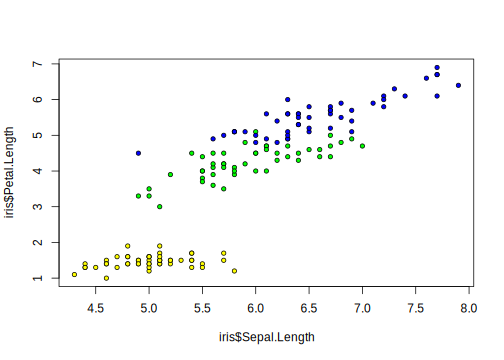
\includegraphics{bot89-introR_files/figure-latex/unnamed-chunk-218-1.pdf}

Muitos argumentos da função \texttt{plot()} são parâmetros gráficos (Seções \ref{par-graficos-p1} e \ref{par-graficos-p2}).

\subsection{Dispositivos de Tela}\label{dispositivos-de-tela}

Quando você usa funções para gerar um gráfico, o R ou RStudio usa automaticamente um dispositivo de tela.
No entanto, você pode abrir novas janelas com as seguintes funções:

\begin{itemize}
\item
  \texttt{X11()} ou \texttt{x11()} funcionam no Mac, Linux e Windows;
\item
  \texttt{quartz()} funciona apenas no Mac;
\item
  \texttt{windows()} funciona apenas no Windows.
\end{itemize}

\begin{Shaded}
\begin{Highlighting}[]
\NormalTok{?device }\CommentTok{\# veja o help da função e as opções de devices}
\FunctionTok{X11}\NormalTok{() }\CommentTok{\# irá abrir uma janela nova}

\CommentTok{\# vamos plotar o mesmo gráfico do exercício anterior}
\NormalTok{vcl }\OtherTok{\textless{}{-}} \FunctionTok{c}\NormalTok{(}\StringTok{"yellow"}\NormalTok{, }\StringTok{"green"}\NormalTok{, }\StringTok{"blue"}\NormalTok{)[}\FunctionTok{as.numeric}\NormalTok{(iris}\SpecialCharTok{$}\NormalTok{Species)] }\CommentTok{\# cria um vetor de cores para cada linha em Iris segundo especie}
\CommentTok{\# plota a figura}
\FunctionTok{plot}\NormalTok{(iris}\SpecialCharTok{$}\NormalTok{Sepal.Length, iris}\SpecialCharTok{$}\NormalTok{Petal.Length, }\AttributeTok{type =} \StringTok{"p"}\NormalTok{, }\AttributeTok{pch =} \DecValTok{21}\NormalTok{, }\AttributeTok{bg =}\NormalTok{ vcl, }\AttributeTok{cex =} \FloatTok{0.8}\NormalTok{)}

\CommentTok{\# irá fechar essa nova janela}
\FunctionTok{dev.off}\NormalTok{()}

\FunctionTok{quartz}\NormalTok{() }\CommentTok{\# num mac abre uma janela sem dar nenhum aviso (funciona melhor que X11() no Mac)}
\NormalTok{vcl }\OtherTok{\textless{}{-}} \FunctionTok{c}\NormalTok{(}\StringTok{"yellow"}\NormalTok{, }\StringTok{"green"}\NormalTok{, }\StringTok{"blue"}\NormalTok{)[}\FunctionTok{as.numeric}\NormalTok{(iris}\SpecialCharTok{$}\NormalTok{Species)] }\CommentTok{\# cria um vetor de cores para cada linha em Iris segundo especie}
\CommentTok{\# plota a figura}
\FunctionTok{plot}\NormalTok{(iris}\SpecialCharTok{$}\NormalTok{Sepal.Length, iris}\SpecialCharTok{$}\NormalTok{Petal.Length, }\AttributeTok{type =} \StringTok{"p"}\NormalTok{, }\AttributeTok{pch =} \DecValTok{21}\NormalTok{, }\AttributeTok{bg =}\NormalTok{ vcl, }\AttributeTok{cex =} \FloatTok{0.8}\NormalTok{)}

\FunctionTok{dev.off}\NormalTok{() }\CommentTok{\# fecha}
\end{Highlighting}
\end{Shaded}

\subsection{Listar e controlar dispositivos}\label{listar-e-controlar-dispositivos}

Existem funções que permitem trabalhar com vários dispositivos ao mesmo tempo, controlando o uso dos dispositivos abertos.
Pode haver, por exemplo, várias janelas diferentes mostrando gráficos diferentes durante um trabalho.
As principais funções para trabalhar com dispositivos são:

\begin{itemize}
\item
  A função \texttt{dev.list()}lista todos os dispositivos abertos no momento (geralmente o dispositivo padrão, que é sempre o número 1, é ignorado na lista), retornando o número (ordem de abertura) e o nome de cada um;
\item
  \texttt{dev.cur()} mostra qual o dispositivo que está ativo (em inglês, \emph{current}). Se há vários abertos, haverá sempre um que estará ativo naquele momento e se você enviar uma figura, ela sairá neste dispositivo;
\item
  \texttt{dev.set()} torna ativo um determinado dispositivo;
\item
  \texttt{dev.off()} fecha o dispositivo atual ou vários. Esta é a função dessa lista que é a mais usada na prática.
\end{itemize}

\begin{Shaded}
\begin{Highlighting}[]
\CommentTok{\# vamos primeiro fechar todos os dispositivos}
\FunctionTok{dev.off}\NormalTok{(}\AttributeTok{which =} \FunctionTok{dev.list}\NormalTok{())}
\FunctionTok{dev.list}\NormalTok{() }\CommentTok{\# vai retornar NULL por não há dispositivos abertos}
\CommentTok{\# vamos abrir vários dispositivos}
\FunctionTok{X11}\NormalTok{() }\CommentTok{\# primeira janela extra}
\FunctionTok{X11}\NormalTok{() }\CommentTok{\# segunda janela e mesma figura com cores diferentes}
\FunctionTok{X11}\NormalTok{() }\CommentTok{\# terceira janela e mesma figura com cores diferentes}

\CommentTok{\# coloque e redimensione as janelas para ter as tres visiveis na tua tela e volte aqui.}

\CommentTok{\# veja os dispositivos abertos}
\FunctionTok{dev.list}\NormalTok{()}

\CommentTok{\# qual o atual}
\FunctionTok{dev.cur}\NormalTok{() }\CommentTok{\# o ultimo que abrimos, né}

\FunctionTok{dev.set}\NormalTok{(}\DecValTok{2}\NormalTok{)}
\CommentTok{\# vamos mudar para o segundo e plotar algo}
\FunctionTok{plot}\NormalTok{(iris}\SpecialCharTok{$}\NormalTok{Sepal.Length, iris}\SpecialCharTok{$}\NormalTok{Petal.Length, }\AttributeTok{type =} \StringTok{"p"}\NormalTok{, }\AttributeTok{cex =} \FloatTok{0.8}\NormalTok{)}

\CommentTok{\# vamos mudar para o terceiro e plotar outra coisa}
\FunctionTok{dev.set}\NormalTok{(}\DecValTok{3}\NormalTok{)}
\FunctionTok{dev.cur}\NormalTok{() }\CommentTok{\# deve responder 3}
\NormalTok{vcl }\OtherTok{\textless{}{-}} \FunctionTok{c}\NormalTok{(}\StringTok{"yellow"}\NormalTok{, }\StringTok{"green"}\NormalTok{, }\StringTok{"blue"}\NormalTok{)[}\FunctionTok{as.numeric}\NormalTok{(iris}\SpecialCharTok{$}\NormalTok{Species)]}
\FunctionTok{plot}\NormalTok{(iris}\SpecialCharTok{$}\NormalTok{Sepal.Length, iris}\SpecialCharTok{$}\NormalTok{Petal.Length, }\AttributeTok{type =} \StringTok{"p"}\NormalTok{, }\AttributeTok{pch =} \DecValTok{21}\NormalTok{, }\AttributeTok{bg =}\NormalTok{ vcl, }\AttributeTok{cex =} \FloatTok{0.8}\NormalTok{)}

\CommentTok{\# vamos mudar para o quarto e plotar a mesma coisa com outras cores}
\FunctionTok{dev.set}\NormalTok{(}\DecValTok{4}\NormalTok{)}
\FunctionTok{dev.cur}\NormalTok{() }\CommentTok{\# deve responder 4}
\NormalTok{vcl }\OtherTok{\textless{}{-}} \FunctionTok{c}\NormalTok{(}\StringTok{"red"}\NormalTok{, }\StringTok{"blue"}\NormalTok{, }\StringTok{"white"}\NormalTok{)[}\FunctionTok{as.numeric}\NormalTok{(iris}\SpecialCharTok{$}\NormalTok{Species)]}
\FunctionTok{plot}\NormalTok{(iris}\SpecialCharTok{$}\NormalTok{Sepal.Length, iris}\SpecialCharTok{$}\NormalTok{Petal.Length, }\AttributeTok{type =} \StringTok{"p"}\NormalTok{, }\AttributeTok{pch =} \DecValTok{21}\NormalTok{, }\AttributeTok{bg =}\NormalTok{ vcl, }\AttributeTok{cex =} \FloatTok{0.8}\NormalTok{)}

\CommentTok{\# vamos fechar o dispositivo atual}
\FunctionTok{dev.cur}\NormalTok{()}
\FunctionTok{dev.off}\NormalTok{()}
\FunctionTok{dev.cur}\NormalTok{() }\CommentTok{\# mudou automaticamente porque voce fechou o 4}
\FunctionTok{dev.off}\NormalTok{() }\CommentTok{\# mesma coisa fechou o ativo}
\FunctionTok{dev.cur}\NormalTok{() }\CommentTok{\# sobrou o 3}
\CommentTok{\# fechar este também}
\FunctionTok{dev.off}\NormalTok{()}
\FunctionTok{dev.list}\NormalTok{() }\CommentTok{\# nao tem mais nenhum aberto}
\end{Highlighting}
\end{Shaded}

\subsection{Dispositivos de arquivos}\label{dispositivos-de-arquivos}

Há vários dispositivos para gerar arquivos com imagens.
As funções em geral têm o nome do tipo de arquivo gerado.
Vamos ver dois exemplos apenas, mas a mesma lógica se aplica a qualquer um dos dispositivos listados no \texttt{?} dos dispositivos (execute o comando \texttt{help(\textquotesingle{}device\textquotesingle{})} e veja a explicação sobre os dispositivos (\emph{devices})).

Essas funções são ótimas ferramentas para incluir nos seus scripts visando a produção de figuras para uma publicação.
Procure na revista em que você deseja publicar seu artigo as especificações técnicas das figuras.
Em seguida, cheque os parâmetros das funções gráficas (Seções \ref{par-graficos-p1} e \ref{par-graficos-p2}) para você ser capaz de gerar figuras na especificação exata da revista selecionada.

\subsection{\texorpdfstring{Figuras vetoriais em \texttt{pdf} ou \texttt{postscript}}{Figuras vetoriais em pdf ou postscript}}\label{figuras-vetoriais-em-pdf-ou-postscript}

Em nossa opinião, as funções \texttt{pdf()} e \texttt{postscript()} são as mais importantes para a geração de figuras, porque elas geram arquivos de excelente qualidade por serem vetoriais.
Não há a necessidade de se definir a resolução, porque nesse tipo de imagem isso não existe.

\begin{Shaded}
\begin{Highlighting}[]
\CommentTok{\# plotando a figura na tela é o que fazemos normalmente}
\NormalTok{vcl }\OtherTok{\textless{}{-}} \FunctionTok{c}\NormalTok{(}\StringTok{"yellow"}\NormalTok{, }\StringTok{"green"}\NormalTok{, }\StringTok{"blue"}\NormalTok{)[}\FunctionTok{as.numeric}\NormalTok{(iris}\SpecialCharTok{$}\NormalTok{Species)]}
\FunctionTok{plot}\NormalTok{(iris}\SpecialCharTok{$}\NormalTok{Sepal.Length, iris}\SpecialCharTok{$}\NormalTok{Petal.Length, }\AttributeTok{type =} \StringTok{"p"}\NormalTok{, }\AttributeTok{pch =} \DecValTok{21}\NormalTok{, }\AttributeTok{bg =}\NormalTok{ vcl, }\AttributeTok{cex =} \FloatTok{0.8}\NormalTok{)}
\end{Highlighting}
\end{Shaded}

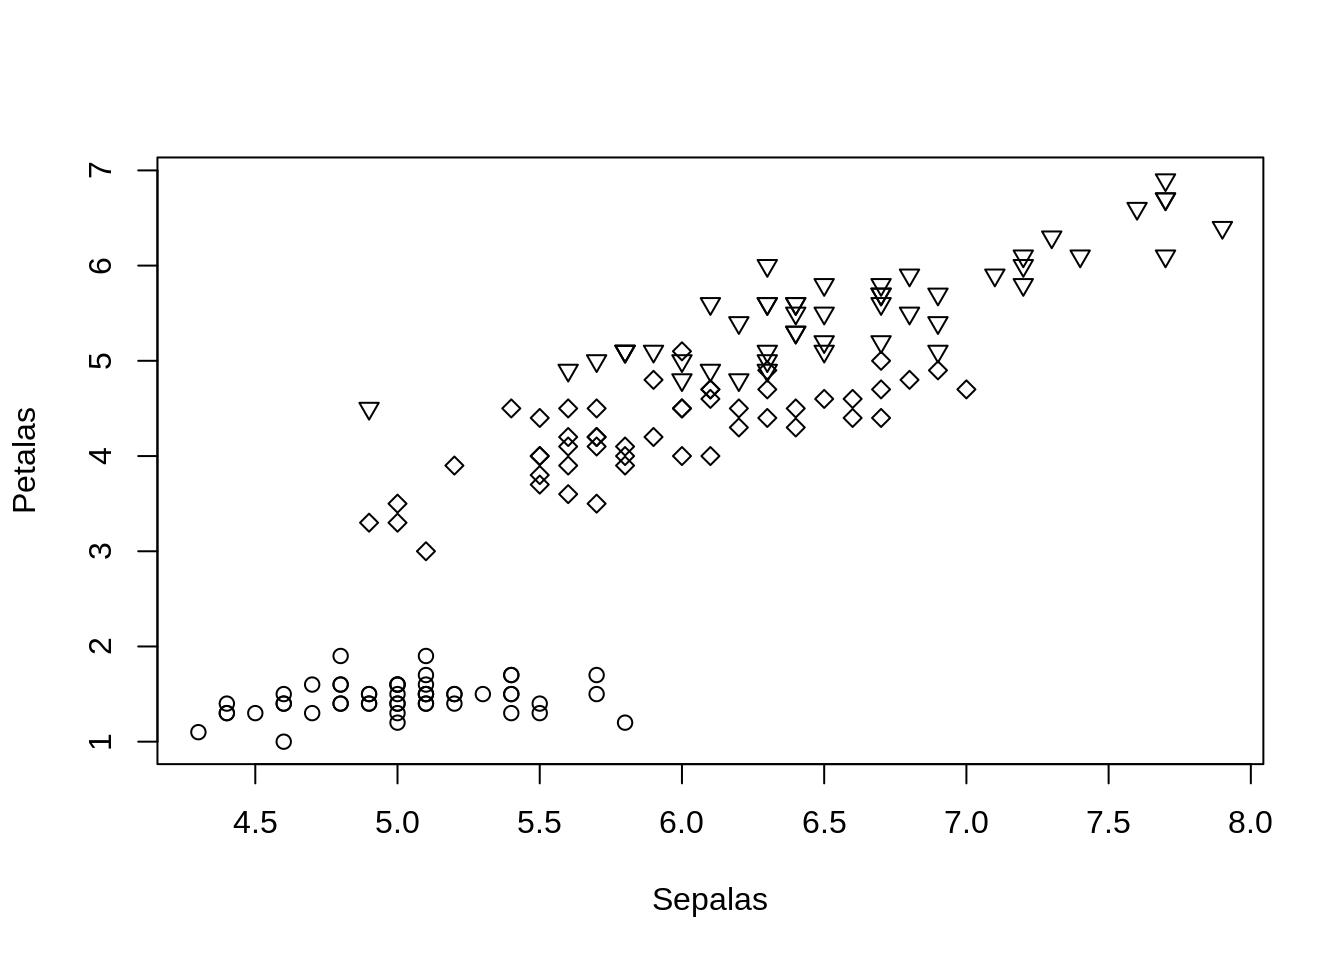
\includegraphics{bot89-introR_files/figure-latex/unnamed-chunk-221-1.pdf}

\begin{Shaded}
\begin{Highlighting}[]
\CommentTok{\# salvando a figura num PDF}
\NormalTok{?pdf }\CommentTok{\# veja o help dessa função e seus argumentos, especialmente width e height}
\CommentTok{\# abre o dispositivo para pdf}
\FunctionTok{pdf}\NormalTok{(}\AttributeTok{file =} \StringTok{"meupdf.pdf"}\NormalTok{, }\AttributeTok{width =} \FunctionTok{lcm}\NormalTok{(}\DecValTok{15}\NormalTok{), }\AttributeTok{height =} \FunctionTok{lcm}\NormalTok{(}\DecValTok{10}\NormalTok{))}
\CommentTok{\# lcm() apenas pega valores em cm e converte em polegadas que é a especificação padrão da funcao pdf. Portanto largura e altura de cada página do PDF é definida por esses argumentos}
\CommentTok{\# plota a figura}
\FunctionTok{plot}\NormalTok{(iris}\SpecialCharTok{$}\NormalTok{Sepal.Length, iris}\SpecialCharTok{$}\NormalTok{Petal.Length, }\AttributeTok{type =} \StringTok{"p"}\NormalTok{, }\AttributeTok{pch =} \DecValTok{21}\NormalTok{, }\AttributeTok{bg =}\NormalTok{ vcl, }\AttributeTok{cex =} \FloatTok{0.8}\NormalTok{)}
\FunctionTok{dev.off}\NormalTok{() }\CommentTok{\# fecha o pdf}
\CommentTok{\# só será possível ver o pdf se tiver fechado ele.}
\FunctionTok{getwd}\NormalTok{() }\CommentTok{\# o pdf foi gerado nessa pasta}

\CommentTok{\# se voce incluir vários gráficos. O pdf irá gerar várias páginas ao mesmo tempo.}
\CommentTok{\# abre o dispositivo para pdf}
\FunctionTok{pdf}\NormalTok{(}\AttributeTok{file =} \StringTok{"meupdf2.pdf"}\NormalTok{, }\AttributeTok{paper =} \StringTok{"a4"}\NormalTok{)}
\CommentTok{\# tamanho papel A4}
\CommentTok{\# plota a figura 10 vezes}
\ControlFlowTok{for}\NormalTok{ (i }\ControlFlowTok{in} \DecValTok{1}\SpecialCharTok{:}\DecValTok{10}\NormalTok{) \{}
  \FunctionTok{plot}\NormalTok{(iris}\SpecialCharTok{$}\NormalTok{Sepal.Length, iris}\SpecialCharTok{$}\NormalTok{Petal.Length, }\AttributeTok{type =} \StringTok{"p"}\NormalTok{, }\AttributeTok{pch =} \DecValTok{21}\NormalTok{, }\AttributeTok{bg =}\NormalTok{ vcl, }\AttributeTok{cex =} \FloatTok{0.8}\NormalTok{)}
\NormalTok{\}}
\FunctionTok{dev.off}\NormalTok{() }\CommentTok{\# fecha o pdf}
\CommentTok{\# veja que o arquivo 2 tem várias páginas}
\end{Highlighting}
\end{Shaded}

\subsection{Figuras raster}\label{figuras-raster}

As funções \texttt{jpeg()}, \texttt{png()} e \texttt{tiff()} geram imagens em pixels, cuja qualidade depende muito da definição da resolução.

\begin{Shaded}
\begin{Highlighting}[]
\CommentTok{\# formato jpeg sem controlar a resolucao (usando units=\textquotesingle{}px\textquotesingle{} ou pixel)}
\CommentTok{\# abre o dispositivo no formato desejado}
\FunctionTok{jpeg}\NormalTok{(}\AttributeTok{filename =} \StringTok{"meujpeg.jpg"}\NormalTok{, }\AttributeTok{width =} \DecValTok{600}\NormalTok{, }\AttributeTok{height =} \DecValTok{400}\NormalTok{, }\AttributeTok{units =} \StringTok{"px"}\NormalTok{)}

\CommentTok{\# plota alguma coisa}
\NormalTok{vcl }\OtherTok{\textless{}{-}} \FunctionTok{c}\NormalTok{(}\StringTok{"yellow"}\NormalTok{, }\StringTok{"green"}\NormalTok{, }\StringTok{"blue"}\NormalTok{)[}\FunctionTok{as.numeric}\NormalTok{(iris}\SpecialCharTok{$}\NormalTok{Species)]}
\FunctionTok{plot}\NormalTok{(iris}\SpecialCharTok{$}\NormalTok{Sepal.Length, iris}\SpecialCharTok{$}\NormalTok{Petal.Length, }\AttributeTok{type =} \StringTok{"p"}\NormalTok{, }\AttributeTok{pch =} \DecValTok{21}\NormalTok{, }\AttributeTok{bg =}\NormalTok{ vcl, }\AttributeTok{cex =} \FloatTok{0.8}\NormalTok{)}

\CommentTok{\# fecha o jpeg}
\FunctionTok{dev.off}\NormalTok{()}

\CommentTok{\# ABRA O ARQUIVO E FAÇA UM ZOOM GRANDE}
\CommentTok{\# note que os pixels são super visíveis}

\CommentTok{\# AGORA MELHORANDO A RESOLUCAO}
\CommentTok{\# formato jpeg com 300dpi}
\CommentTok{\# abre o dispositivo no formato desejado}
\FunctionTok{jpeg}\NormalTok{(}\AttributeTok{filename =} \StringTok{"meujpeg2.jpg"}\NormalTok{, }\AttributeTok{width =} \DecValTok{15}\NormalTok{, }\AttributeTok{height =} \DecValTok{10}\NormalTok{, }\AttributeTok{units =} \StringTok{"cm"}\NormalTok{, }\AttributeTok{res =} \DecValTok{300}\NormalTok{)}

\CommentTok{\# plota alguma coisa}
\NormalTok{vcl }\OtherTok{\textless{}{-}} \FunctionTok{c}\NormalTok{(}\StringTok{"yellow"}\NormalTok{, }\StringTok{"green"}\NormalTok{, }\StringTok{"blue"}\NormalTok{)[}\FunctionTok{as.numeric}\NormalTok{(iris}\SpecialCharTok{$}\NormalTok{Species)]}
\FunctionTok{plot}\NormalTok{(iris}\SpecialCharTok{$}\NormalTok{Sepal.Length, iris}\SpecialCharTok{$}\NormalTok{Petal.Length, }\AttributeTok{type =} \StringTok{"p"}\NormalTok{, }\AttributeTok{pch =} \DecValTok{21}\NormalTok{, }\AttributeTok{bg =}\NormalTok{ vcl, }\AttributeTok{cex =} \FloatTok{0.8}\NormalTok{)}

\CommentTok{\# fecha o jpeg}
\FunctionTok{dev.off}\NormalTok{()}
\end{Highlighting}
\end{Shaded}

\begin{rmdidea}
DICA: Abra os três arquivos e compare a resolução deles, ampliando a
imagem até visualizar o pixel. Note que em um \texttt{pdf} você nunca
verá o pixel. Por isso, recomendamos que vocÊ trabalhe sempre com a
função \texttt{pdf()}.
\end{rmdidea}

\section{Parâmetros gráficos, parte I - Margem, fonte, proporções}\label{par-graficos-p1}

Para fazer boas figuras no R, você precisa muitas vezes controlar \textbf{parâmetros gráficos dos dispositivos}, como margem da figura, tamanho de fonte, tipo da fonte, distância das legendas dos eixos x e y, se essas legendas são horizontais ou verticais, o tipo símbolos dos pontos, as cores dos simbolos etc.
Você pode definir esses parâmetros diretamente nas funções gráficas de alto-nível \texttt{highlevel\ plot\textgreater{}\ (...,\ \textless{}tag\textgreater{}\ =\ \textless{}value\textgreater{})}, onde um valor (value) de um parâmetro (tag) pode ser adicionado diretamente como argumento de uma função de alto-nível.

Alguns desses parâmetros, no entanto, só podem ser definidos através da função \texttt{par()}, que também define \textbf{parâmetros gráficos globais}, isto é, se você alterar os parâmetros através dessa função, isso será alterado para todos os gráficos que forem abertos posteriormente durante a mesma sessão do R.
Esta mesma função também permite visualizar os parâmetros gráficos.

Leia atentamente o \texttt{?} da função \href{http://stat.ethz.ch/R-manual/R-devel/library/graphics/html/par.html}{\texttt{par()}}.
Você pode salvar os parâmetros globais antes de alterá-los.

\begin{Shaded}
\begin{Highlighting}[]
\NormalTok{?par }\CommentTok{\# veja o help dessa função}
\end{Highlighting}
\end{Shaded}

\begin{Shaded}
\begin{Highlighting}[]
\CommentTok{\# você pode ver os parâmetros padrão:}
\FunctionTok{par}\NormalTok{() }\CommentTok{\# vejo todos os parâmetros}
\end{Highlighting}
\end{Shaded}

\begin{verbatim}
## $xlog
## [1] FALSE
## 
## $ylog
## [1] FALSE
## 
## $adj
## [1] 0.5
## 
## $ann
## [1] TRUE
## 
## $ask
## [1] FALSE
## 
## $bg
## [1] "white"
## 
## $bty
## [1] "o"
## 
## $cex
## [1] 1
## 
## $cex.axis
## [1] 1
## 
## $cex.lab
## [1] 1
## 
## $cex.main
## [1] 1.2
## 
## $cex.sub
## [1] 1
## 
## $cin
## [1] 0.15 0.20
## 
## $col
## [1] "black"
## 
## $col.axis
## [1] "black"
## 
## $col.lab
## [1] "black"
## 
## $col.main
## [1] "black"
## 
## $col.sub
## [1] "black"
## 
## $cra
## [1] 10.8 14.4
## 
## $crt
## [1] 0
## 
## $csi
## [1] 0.2
## 
## $cxy
## [1] 0.02851711 0.07518797
## 
## $din
## [1] 6.5 4.5
## 
## $err
## [1] 0
## 
## $family
## [1] ""
## 
## $fg
## [1] "black"
## 
## $fig
## [1] 0 1 0 1
## 
## $fin
## [1] 6.5 4.5
## 
## $font
## [1] 1
## 
## $font.axis
## [1] 1
## 
## $font.lab
## [1] 1
## 
## $font.main
## [1] 2
## 
## $font.sub
## [1] 1
## 
## $lab
## [1] 5 5 7
## 
## $las
## [1] 0
## 
## $lend
## [1] "round"
## 
## $lheight
## [1] 1
## 
## $ljoin
## [1] "round"
## 
## $lmitre
## [1] 10
## 
## $lty
## [1] "solid"
## 
## $lwd
## [1] 1
## 
## $mai
## [1] 1.02 0.82 0.82 0.42
## 
## $mar
## [1] 5.1 4.1 4.1 2.1
## 
## $mex
## [1] 1
## 
## $mfcol
## [1] 1 1
## 
## $mfg
## [1] 1 1 1 1
## 
## $mfrow
## [1] 1 1
## 
## $mgp
## [1] 3 1 0
## 
## $mkh
## [1] 0.001
## 
## $new
## [1] FALSE
## 
## $oma
## [1] 0 0 0 0
## 
## $omd
## [1] 0 1 0 1
## 
## $omi
## [1] 0 0 0 0
## 
## $page
## [1] TRUE
## 
## $pch
## [1] 1
## 
## $pin
## [1] 5.26 2.66
## 
## $plt
## [1] 0.1261538 0.9353846 0.2266667 0.8177778
## 
## $ps
## [1] 12
## 
## $pty
## [1] "m"
## 
## $smo
## [1] 1
## 
## $srt
## [1] 0
## 
## $tck
## [1] NA
## 
## $tcl
## [1] -0.5
## 
## $usr
## [1] 0 1 0 1
## 
## $xaxp
## [1] 0 1 5
## 
## $xaxs
## [1] "r"
## 
## $xaxt
## [1] "s"
## 
## $xpd
## [1] FALSE
## 
## $yaxp
## [1] 0 1 5
## 
## $yaxs
## [1] "r"
## 
## $yaxt
## [1] "s"
## 
## $ylbias
## [1] 0.2
\end{verbatim}

\begin{Shaded}
\begin{Highlighting}[]
\NormalTok{op }\OtherTok{\textless{}{-}} \FunctionTok{par}\NormalTok{() }\CommentTok{\# pego todos os parâmetros}
\FunctionTok{class}\NormalTok{(op) }\CommentTok{\# isso é uma lista}
\end{Highlighting}
\end{Shaded}

\begin{verbatim}
## [1] "list"
\end{verbatim}

\begin{Shaded}
\begin{Highlighting}[]
\FunctionTok{names}\NormalTok{(op) }\CommentTok{\# esses são os nomes dos parâmetros}
\end{Highlighting}
\end{Shaded}

\begin{verbatim}
##  [1] "xlog"      "ylog"      "adj"       "ann"       "ask"       "bg"       
##  [7] "bty"       "cex"       "cex.axis"  "cex.lab"   "cex.main"  "cex.sub"  
## [13] "cin"       "col"       "col.axis"  "col.lab"   "col.main"  "col.sub"  
## [19] "cra"       "crt"       "csi"       "cxy"       "din"       "err"      
## [25] "family"    "fg"        "fig"       "fin"       "font"      "font.axis"
## [31] "font.lab"  "font.main" "font.sub"  "lab"       "las"       "lend"     
## [37] "lheight"   "ljoin"     "lmitre"    "lty"       "lwd"       "mai"      
## [43] "mar"       "mex"       "mfcol"     "mfg"       "mfrow"     "mgp"      
## [49] "mkh"       "new"       "oma"       "omd"       "omi"       "page"     
## [55] "pch"       "pin"       "plt"       "ps"        "pty"       "smo"      
## [61] "srt"       "tck"       "tcl"       "usr"       "xaxp"      "xaxs"     
## [67] "xaxt"      "xpd"       "yaxp"      "yaxs"      "yaxt"      "ylbias"
\end{verbatim}

\begin{Shaded}
\begin{Highlighting}[]
\CommentTok{\# a função par permite ver os valores atualmente definidos}
\FunctionTok{par}\NormalTok{(}\StringTok{"family"}\NormalTok{) }\CommentTok{\# tipo de fonte nao tem}
\end{Highlighting}
\end{Shaded}

\begin{verbatim}
## [1] ""
\end{verbatim}

\begin{Shaded}
\begin{Highlighting}[]
\FunctionTok{par}\NormalTok{(}\StringTok{"mar"}\NormalTok{) }\CommentTok{\# margens da figura em número de linhas}
\end{Highlighting}
\end{Shaded}

\begin{verbatim}
## [1] 5.1 4.1 4.1 2.1
\end{verbatim}

\begin{Shaded}
\begin{Highlighting}[]
\CommentTok{\# a função para tem apenas 1 argumento além dos parâmetros gráficos}
\NormalTok{op2 }\OtherTok{\textless{}{-}} \FunctionTok{par}\NormalTok{(}\AttributeTok{no.readonly =} \ConstantTok{TRUE}\NormalTok{)}
\FunctionTok{class}\NormalTok{(op2)}
\end{Highlighting}
\end{Shaded}

\begin{verbatim}
## [1] "list"
\end{verbatim}

\begin{Shaded}
\begin{Highlighting}[]
\CommentTok{\# a diferença entre especificar no.readonly como verdadeiro (na primeria opção não especificada acima, o padrão é FALSE)}
\CommentTok{\# é que a lista gerada pode ser usada para refazer alterações, ou seja, para resgatar os parâmetros gráficos padrão.}

\CommentTok{\# ou seja, posso fazer:}
\FunctionTok{par}\NormalTok{(op2) }\CommentTok{\# para resgatar valores originais}
\end{Highlighting}
\end{Shaded}

\begin{Shaded}
\begin{Highlighting}[]
\CommentTok{\# mas não posso fazer o mesmo com a primeira opção}
\FunctionTok{par}\NormalTok{(op) }\CommentTok{\# porque op é uma lista diferente}
\end{Highlighting}
\end{Shaded}

\begin{Shaded}
\begin{Highlighting}[]
\FunctionTok{length}\NormalTok{(op) }\SpecialCharTok{==} \FunctionTok{length}\NormalTok{(op2) }\CommentTok{\# tem comprimentos diferentes}
\end{Highlighting}
\end{Shaded}

\begin{verbatim}
## [1] FALSE
\end{verbatim}

\begin{Shaded}
\begin{Highlighting}[]
\FunctionTok{identical}\NormalTok{(op, op2) }\CommentTok{\# nao são identicas}
\end{Highlighting}
\end{Shaded}

\begin{verbatim}
## [1] FALSE
\end{verbatim}

\subsection{Margem da figura}\label{margem-da-figura}

\begin{Shaded}
\begin{Highlighting}[]
\CommentTok{\# Usando novamente o exemplo de iris}
\NormalTok{Sepalas }\OtherTok{\textless{}{-}}\NormalTok{ iris}\SpecialCharTok{$}\NormalTok{Sepal.Length}
\NormalTok{Petalas }\OtherTok{\textless{}{-}}\NormalTok{ iris}\SpecialCharTok{$}\NormalTok{Petal.Length}

\CommentTok{\# especies como números}
\NormalTok{spp }\OtherTok{\textless{}{-}} \FunctionTok{as.numeric}\NormalTok{(}\FunctionTok{as.factor}\NormalTok{(iris}\SpecialCharTok{$}\NormalTok{Species))}
\CommentTok{\# uma cor para cada espécie}
\NormalTok{vcl }\OtherTok{\textless{}{-}} \FunctionTok{c}\NormalTok{(}\StringTok{"yellow"}\NormalTok{, }\StringTok{"green"}\NormalTok{, }\StringTok{"blue"}\NormalTok{)[spp]}
\CommentTok{\# um simbolo para cada espécie}
\NormalTok{sbs }\OtherTok{\textless{}{-}} \FunctionTok{c}\NormalTok{(}\DecValTok{21}\NormalTok{, }\DecValTok{22}\NormalTok{, }\DecValTok{23}\NormalTok{)[spp]}

\CommentTok{\# plota a figura no dispositivo padrão}
\FunctionTok{plot}\NormalTok{(Sepalas,}
\NormalTok{  Petalas,}
  \AttributeTok{pch =}\NormalTok{ sbs,}
  \AttributeTok{bg =}\NormalTok{ vcl,}
  \AttributeTok{cex =} \FloatTok{0.8}
\NormalTok{)}
\end{Highlighting}
\end{Shaded}

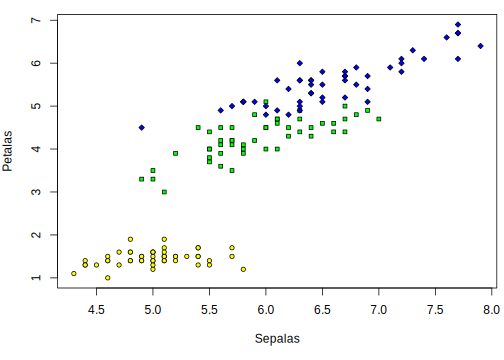
\includegraphics{bot89-introR_files/figure-latex/unnamed-chunk-229-1.pdf}

\begin{Shaded}
\begin{Highlighting}[]
\CommentTok{\# ALTERANDO A MARGEM em NUMEROS DE LINHAS}
\CommentTok{\# salva o valor padrao para resgatar ao final}
\NormalTok{op }\OtherTok{\textless{}{-}} \FunctionTok{par}\NormalTok{(}\AttributeTok{no.readonly =} \ConstantTok{TRUE}\NormalTok{)}
\NormalTok{op}\SpecialCharTok{$}\NormalTok{mar }\CommentTok{\# esses são os valor atuais para Margem Inferior, Esquerda, Superior e Direita, respectivamente. \#quando se referir a margem todos os parâmetros seguem a ordem ANTI{-}HORÁRIA iniciando na margem inferior}
\end{Highlighting}
\end{Shaded}

\begin{verbatim}
## [1] 5.1 4.1 4.1 2.1
\end{verbatim}

\begin{Shaded}
\begin{Highlighting}[]
\CommentTok{\# reduzindo as margem direita e superior em número de linhas}
\FunctionTok{par}\NormalTok{(}\AttributeTok{mar =} \FunctionTok{c}\NormalTok{(}\DecValTok{5}\NormalTok{, }\DecValTok{4}\NormalTok{, }\DecValTok{1}\NormalTok{, }\FloatTok{0.5}\NormalTok{))}
\FunctionTok{plot}\NormalTok{(Sepalas,}
\NormalTok{  Petalas,}
  \AttributeTok{pch =}\NormalTok{ sbs,}
  \AttributeTok{bg =}\NormalTok{ vcl,}
  \AttributeTok{cex =} \FloatTok{0.8}
\NormalTok{)}

\CommentTok{\# voltando ao original}
\FunctionTok{par}\NormalTok{(}\AttributeTok{mar =}\NormalTok{ op}\SpecialCharTok{$}\NormalTok{mar)}
\end{Highlighting}
\end{Shaded}

\subsection{Aspecto dos eixos}\label{aspecto-dos-eixos}

\begin{Shaded}
\begin{Highlighting}[]
\NormalTok{op }\OtherTok{\textless{}{-}} \FunctionTok{par}\NormalTok{(}\AttributeTok{no.readonly =} \ConstantTok{TRUE}\NormalTok{)}


\CommentTok{\# POSICAO DAS LEGENDAS DOS EIXOS}
\FunctionTok{par}\NormalTok{(}\StringTok{"mgp"}\NormalTok{) }\CommentTok{\# três valores que correspondem ao número de linhas para: (1) Titulo dos Eixos; (2) valores dos eixos; (3) linha dos eixos}

\CommentTok{\# TAMANHO DE FONTE DOS EIXOS É RELATIVO AO VALOR DE FONTE PADRÃO}
\FunctionTok{par}\NormalTok{(}\StringTok{"cex"}\NormalTok{) }\CommentTok{\# tamanho padrão}
\FunctionTok{par}\NormalTok{(}\StringTok{"cex.lab"}\NormalTok{) }\CommentTok{\# número que multiplicado por op$cex indica o valor da fonte dos títulos dos eixos}
\FunctionTok{par}\NormalTok{(}\StringTok{"cex.axis"}\NormalTok{) }\CommentTok{\# dos valores}


\CommentTok{\# TAMANHO DAS BARRAS DE CADA VALOR}
\FunctionTok{par}\NormalTok{(}\StringTok{"tck"}\NormalTok{) }\CommentTok{\# geralmente não tem padrão definido pois é extraído de outros valores automaticamente, mas você pode controlar isso}

\CommentTok{\# DIMINUINDO A FONTE DISSO}
\FunctionTok{par}\NormalTok{(}\AttributeTok{cex.lab =} \FloatTok{0.8}\NormalTok{, }\AttributeTok{cex.axis =} \FloatTok{0.7}\NormalTok{)}
\FunctionTok{plot}\NormalTok{(Sepalas, Petalas, }\AttributeTok{pch =}\NormalTok{ sbs, }\AttributeTok{bg =}\NormalTok{ vcl, }\AttributeTok{cex =} \FloatTok{0.8}\NormalTok{)}

\CommentTok{\# note que isso muda se eu alterar o tamanho de fonte padrão par(cex)}
\FunctionTok{par}\NormalTok{(}\AttributeTok{cex =} \DecValTok{2}\NormalTok{, }\AttributeTok{cex.lab =} \FloatTok{0.8}\NormalTok{, }\AttributeTok{cex.axis =} \FloatTok{0.7}\NormalTok{)}
\FunctionTok{plot}\NormalTok{(Sepalas, Petalas, }\AttributeTok{pch =}\NormalTok{ sbs, }\AttributeTok{bg =}\NormalTok{ vcl, }\AttributeTok{cex =} \FloatTok{0.8}\NormalTok{)}

\CommentTok{\# APROXIMANDO}
\FunctionTok{par}\NormalTok{(}\AttributeTok{mgp =} \FunctionTok{c}\NormalTok{(}\FloatTok{1.5}\NormalTok{, }\FloatTok{0.5}\NormalTok{, }\DecValTok{0}\NormalTok{))}
\FunctionTok{plot}\NormalTok{(Sepalas, Petalas, }\AttributeTok{pch =}\NormalTok{ sbs, }\AttributeTok{bg =}\NormalTok{ vcl, }\AttributeTok{cex =} \FloatTok{0.8}\NormalTok{)}

\CommentTok{\# e agora}
\FunctionTok{par}\NormalTok{(}\AttributeTok{tck =} \SpecialCharTok{{-}}\FloatTok{0.01}\NormalTok{) }\CommentTok{\# note o valor negativo}
\FunctionTok{plot}\NormalTok{(Sepalas, Petalas, }\AttributeTok{pch =}\NormalTok{ sbs, }\AttributeTok{bg =}\NormalTok{ vcl, }\AttributeTok{cex =} \FloatTok{0.8}\NormalTok{)}

\FunctionTok{par}\NormalTok{(}\AttributeTok{tck =} \FloatTok{0.01}\NormalTok{) }\CommentTok{\# se colocar positivo}
\FunctionTok{plot}\NormalTok{(Sepalas, Petalas, }\AttributeTok{pch =}\NormalTok{ sbs, }\AttributeTok{bg =}\NormalTok{ vcl, }\AttributeTok{cex =} \FloatTok{0.8}\NormalTok{)}

\FunctionTok{par}\NormalTok{(op) }\CommentTok{\# restaurando valores originais}
\FunctionTok{plot}\NormalTok{(Sepalas, Petalas, }\AttributeTok{pch =}\NormalTok{ sbs, }\AttributeTok{bg =}\NormalTok{ vcl, }\AttributeTok{cex =} \FloatTok{0.8}\NormalTok{)}
\end{Highlighting}
\end{Shaded}

\subsection{Proporção dos eixos}\label{proporuxe7uxe3o-dos-eixos}

\begin{Shaded}
\begin{Highlighting}[]
\NormalTok{op }\OtherTok{\textless{}{-}} \FunctionTok{par}\NormalTok{(}\AttributeTok{no.readonly =} \ConstantTok{TRUE}\NormalTok{)}

\FunctionTok{par}\NormalTok{(}\StringTok{"pty"}\NormalTok{) }\CommentTok{\# valor "m" maximiza a area disponível}
\end{Highlighting}
\end{Shaded}

\begin{verbatim}
## [1] "m"
\end{verbatim}

\begin{Shaded}
\begin{Highlighting}[]
\FunctionTok{plot}\NormalTok{(Sepalas, Petalas, }\AttributeTok{pch =}\NormalTok{ sbs, }\AttributeTok{bg =}\NormalTok{ vcl, }\AttributeTok{cex =} \FloatTok{0.8}\NormalTok{)}
\end{Highlighting}
\end{Shaded}

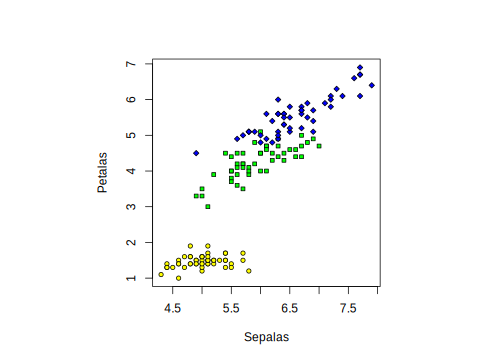
\includegraphics{bot89-introR_files/figure-latex/unnamed-chunk-231-1.pdf}

\begin{Shaded}
\begin{Highlighting}[]
\CommentTok{\# agora mantendo a proporção dos eixos (sem esticar nenhum dos dois)}
\FunctionTok{par}\NormalTok{(}\AttributeTok{pty =} \StringTok{"s"}\NormalTok{)}
\FunctionTok{plot}\NormalTok{(Sepalas, Petalas, }\AttributeTok{pch =}\NormalTok{ sbs, }\AttributeTok{bg =}\NormalTok{ vcl, }\AttributeTok{cex =} \FloatTok{0.8}\NormalTok{)}

\CommentTok{\# se não notou diferença, expandir o dispositivo onde está desenhando a figura}
\end{Highlighting}
\end{Shaded}

\subsection{\texorpdfstring{Múltiplas figuras na mesma tela ou página com \texttt{mfrow()} e \texttt{mfcol()}}{Múltiplas figuras na mesma tela ou página com mfrow() e mfcol()}}\label{muxfaltiplas-figuras-na-mesma-tela-ou-puxe1gina-com-mfrow-e-mfcol}

Você pode colocar diferentes gráficos na mesma tela ou na mesma página de um pdf, por exemplo. Temos duas formas de fazer isso.
Os parâmetros \texttt{mfrow} e \texttt{mfcol} dividem os dispositivo em células de tamanhos idênticos.
Todas as figuras terão o mesmo tamanho.
A diferença entre os dois parâmetros é que \texttt{mfrow()} preenche o espaço por linhas, enquanto \texttt{mfcol()} preenche o espaço pelas colunas.

\begin{Shaded}
\begin{Highlighting}[]
\FunctionTok{par}\NormalTok{(op)}
\FunctionTok{par}\NormalTok{(}\StringTok{"mfrow"}\NormalTok{) }\CommentTok{\# o dispositivo não está divido: tem 1 linha e 1 coluna}
\end{Highlighting}
\end{Shaded}

\begin{verbatim}
## [1] 1 1
\end{verbatim}

\begin{Shaded}
\begin{Highlighting}[]
\FunctionTok{plot}\NormalTok{(Sepalas, Petalas, }\AttributeTok{pch =}\NormalTok{ sbs, }\AttributeTok{bg =}\NormalTok{ vcl, }\AttributeTok{cex =} \FloatTok{0.8}\NormalTok{)}

\CommentTok{\# EXEMPLO 1}
\CommentTok{\# duas figuras no mesmo dispositivo}
\FunctionTok{par}\NormalTok{(}\AttributeTok{mfrow =} \FunctionTok{c}\NormalTok{(}\DecValTok{1}\NormalTok{, }\DecValTok{2}\NormalTok{)) }\CommentTok{\# dividir o dispositivo em 1 linha e duas colunas}
\CommentTok{\# plota a primeira figura}
\FunctionTok{plot}\NormalTok{(Sepalas, Petalas, }\AttributeTok{pch =}\NormalTok{ sbs, }\AttributeTok{bg =}\NormalTok{ vcl, }\AttributeTok{cex =} \FloatTok{0.8}\NormalTok{)}
\CommentTok{\# plota a segunda sem cores}
\FunctionTok{plot}\NormalTok{(Sepalas, Petalas, }\AttributeTok{pch =}\NormalTok{ sbs, }\AttributeTok{bg =} \ConstantTok{NULL}\NormalTok{, }\AttributeTok{cex =} \FloatTok{0.8}\NormalTok{)}
\end{Highlighting}
\end{Shaded}

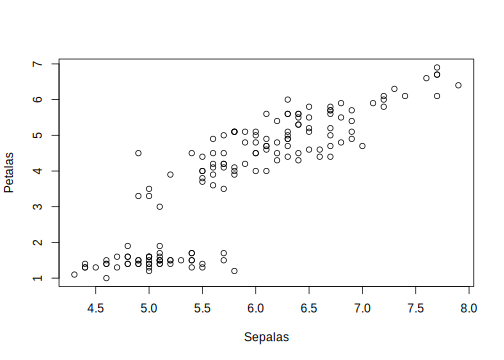
\includegraphics{bot89-introR_files/figure-latex/unnamed-chunk-232-1.pdf}

\begin{Shaded}
\begin{Highlighting}[]
\CommentTok{\# EXEMPLO 2}
\FunctionTok{par}\NormalTok{(}\AttributeTok{mar =} \FunctionTok{c}\NormalTok{(}\FloatTok{5.1}\NormalTok{, }\FloatTok{4.1}\NormalTok{, }\FloatTok{2.1}\NormalTok{, }\FloatTok{2.1}\NormalTok{))}
\FunctionTok{par}\NormalTok{(}\AttributeTok{mfrow =} \FunctionTok{c}\NormalTok{(}\DecValTok{2}\NormalTok{, }\DecValTok{2}\NormalTok{)) }\CommentTok{\# dividir o dispositivo em 2 linha e duas colunas}
\CommentTok{\# plota quatro figuras identificas}
\ControlFlowTok{for}\NormalTok{ (f }\ControlFlowTok{in} \DecValTok{1}\SpecialCharTok{:}\DecValTok{4}\NormalTok{) \{}
  \FunctionTok{plot}\NormalTok{(Sepalas, Petalas, }\AttributeTok{pch =}\NormalTok{ sbs, }\AttributeTok{bg =} \ConstantTok{NULL}\NormalTok{, }\AttributeTok{cex =} \FloatTok{0.8}\NormalTok{)}
  \CommentTok{\# adiciona uma letra para você ver a ordem e comparar com o exemplo 3}
  \FunctionTok{mtext}\NormalTok{(LETTERS[f], }\AttributeTok{side =} \DecValTok{3}\NormalTok{, }\AttributeTok{line =} \DecValTok{0}\NormalTok{, }\AttributeTok{adj =} \DecValTok{0}\NormalTok{, }\AttributeTok{font =} \DecValTok{2}\NormalTok{, }\AttributeTok{col =} \StringTok{"red"}\NormalTok{) }\CommentTok{\# esta é uma função de baixo nível que falaremos depois}
\NormalTok{\}}
\end{Highlighting}
\end{Shaded}

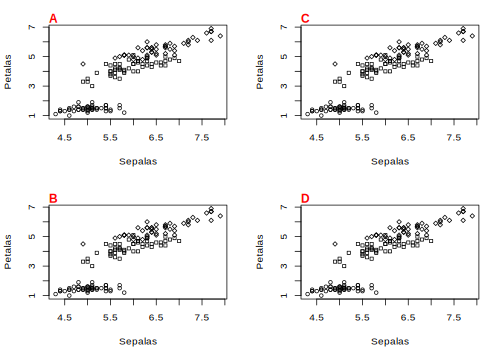
\includegraphics{bot89-introR_files/figure-latex/unnamed-chunk-232-2.pdf}

\begin{Shaded}
\begin{Highlighting}[]
\CommentTok{\# EXEMPLO 3}
\FunctionTok{par}\NormalTok{(}\AttributeTok{mfcol =} \FunctionTok{c}\NormalTok{(}\DecValTok{2}\NormalTok{, }\DecValTok{2}\NormalTok{)) }\CommentTok{\# mesma coisa mas preenchendo por colunas (compare com a figura acima)}
\ControlFlowTok{for}\NormalTok{ (f }\ControlFlowTok{in} \DecValTok{1}\SpecialCharTok{:}\DecValTok{4}\NormalTok{) \{}
  \FunctionTok{plot}\NormalTok{(Sepalas, Petalas, }\AttributeTok{pch =}\NormalTok{ sbs, }\AttributeTok{bg =} \ConstantTok{NULL}\NormalTok{, }\AttributeTok{cex =} \FloatTok{0.8}\NormalTok{)}
  \FunctionTok{mtext}\NormalTok{(LETTERS[f], }\AttributeTok{side =} \DecValTok{3}\NormalTok{, }\AttributeTok{line =} \DecValTok{0}\NormalTok{, }\AttributeTok{adj =} \DecValTok{0}\NormalTok{, }\AttributeTok{font =} \DecValTok{2}\NormalTok{, }\AttributeTok{col =} \StringTok{"red"}\NormalTok{)}
\NormalTok{\}}
\end{Highlighting}
\end{Shaded}

\begin{Shaded}
\begin{Highlighting}[]
\CommentTok{\# colocando exemplo 2 e 3 num pdf}
\FunctionTok{pdf}\NormalTok{(}\AttributeTok{file =} \StringTok{"meuPDFmfrow.pdf"}\NormalTok{, }\AttributeTok{paper =} \StringTok{"a4"}\NormalTok{)}
\CommentTok{\# EXEMPLO 2 expandido}
\FunctionTok{par}\NormalTok{(}\AttributeTok{mfrow =} \FunctionTok{c}\NormalTok{(}\DecValTok{3}\NormalTok{, }\DecValTok{2}\NormalTok{)) }\CommentTok{\# tres linhas e duas colunas}
\ControlFlowTok{for}\NormalTok{ (f }\ControlFlowTok{in} \DecValTok{1}\SpecialCharTok{:}\DecValTok{6}\NormalTok{) \{}
  \FunctionTok{plot}\NormalTok{(Sepalas, Petalas, }\AttributeTok{pch =}\NormalTok{ sbs, }\AttributeTok{bg =} \ConstantTok{NULL}\NormalTok{, }\AttributeTok{cex =} \FloatTok{0.8}\NormalTok{)}
  \FunctionTok{mtext}\NormalTok{(LETTERS[f], }\AttributeTok{side =} \DecValTok{3}\NormalTok{, }\AttributeTok{line =} \DecValTok{0}\NormalTok{, }\AttributeTok{adj =} \DecValTok{0}\NormalTok{, }\AttributeTok{font =} \DecValTok{2}\NormalTok{, }\AttributeTok{col =} \StringTok{"red"}\NormalTok{)}
\NormalTok{\}}
\CommentTok{\# EXEMPLO 3 expandido}
\FunctionTok{par}\NormalTok{(}\AttributeTok{mfcol =} \FunctionTok{c}\NormalTok{(}\DecValTok{3}\NormalTok{, }\DecValTok{2}\NormalTok{))}
\ControlFlowTok{for}\NormalTok{ (f }\ControlFlowTok{in} \DecValTok{1}\SpecialCharTok{:}\DecValTok{6}\NormalTok{) \{}
  \FunctionTok{plot}\NormalTok{(Sepalas, Petalas, }\AttributeTok{pch =}\NormalTok{ sbs, }\AttributeTok{bg =} \ConstantTok{NULL}\NormalTok{, }\AttributeTok{cex =} \FloatTok{0.8}\NormalTok{)}
  \FunctionTok{mtext}\NormalTok{(LETTERS[f], }\AttributeTok{side =} \DecValTok{3}\NormalTok{, }\AttributeTok{line =} \DecValTok{0}\NormalTok{, }\AttributeTok{adj =} \DecValTok{0}\NormalTok{, }\AttributeTok{font =} \DecValTok{2}\NormalTok{, }\AttributeTok{col =} \StringTok{"red"}\NormalTok{)}
\NormalTok{\}}
\FunctionTok{dev.off}\NormalTok{()}
\end{Highlighting}
\end{Shaded}

\subsection{\texorpdfstring{Múltiplas figuras na mesma image usando a função \texttt{layout()}}{Múltiplas figuras na mesma image usando a função layout()}}\label{muxfaltiplas-figuras-na-mesma-image-usando-a-funuxe7uxe3o-layout}

A função \texttt{layout()} também permite dividir um dispositivo para múltiplas figuras, mas de uma forma muito mais complexa.

\begin{Shaded}
\begin{Highlighting}[]
\NormalTok{?layout }\CommentTok{\# veja o help dessa função}

\CommentTok{\# voce precisa definir uma matriz que indica:}
\CommentTok{\# 1) o numero de figuras (valores da matriz)}
\CommentTok{\# 2) a posição das figuras (numero de linhas e colunas)}
\CommentTok{\# por exemplo, suponha que queremos plotar 3 figuras:}
\CommentTok{\# 1 preenchendo a largura da página e metade da altura}
\CommentTok{\# 2 outras figuras preenchendo a outra metada da altura}
\end{Highlighting}
\end{Shaded}

\begin{Shaded}
\begin{Highlighting}[]
\CommentTok{\# neste caso a figura 1 ira ocupar dois espacos}
\NormalTok{mm }\OtherTok{\textless{}{-}} \FunctionTok{matrix}\NormalTok{(}\FunctionTok{c}\NormalTok{(}\DecValTok{1}\NormalTok{, }\DecValTok{1}\NormalTok{, }\DecValTok{2}\NormalTok{, }\DecValTok{3}\NormalTok{), }\AttributeTok{nrow =} \DecValTok{2}\NormalTok{, }\AttributeTok{ncol =} \DecValTok{2}\NormalTok{, }\AttributeTok{byrow =}\NormalTok{ T)}
\NormalTok{mm }\CommentTok{\# a figura 1 irá ocupar a posicao do numero 1 na matriz}
\CommentTok{\# a figura 2 irá ocupar a posicao do numero 2 nessa matriz}
\CommentTok{\# a figura 3 irá ocupar a posicao do numero 3 dessa matriz}
\CommentTok{\# a largura de cada coluna e linha é especificada pelos argumentos widths e heights e usaremos a função lcm() para especificar isso em centímetros}
\CommentTok{\# divide o dispositivo}
\NormalTok{ml }\OtherTok{\textless{}{-}} \FunctionTok{layout}\NormalTok{(mm, }\AttributeTok{widths =} \FunctionTok{rep}\NormalTok{(}\FunctionTok{lcm}\NormalTok{(}\DecValTok{5}\NormalTok{), }\FunctionTok{ncol}\NormalTok{(mm)), }\AttributeTok{heights =} \FunctionTok{rep}\NormalTok{(}\FunctionTok{lcm}\NormalTok{(}\DecValTok{5}\NormalTok{), }\FunctionTok{nrow}\NormalTok{(mm)))}
\CommentTok{\# mostra a divisao feita}
\FunctionTok{layout.show}\NormalTok{(ml)}

\CommentTok{\# plota a primeira figura}
\FunctionTok{plot}\NormalTok{(Sepalas, Petalas, }\AttributeTok{pch =}\NormalTok{ sbs, }\AttributeTok{bg =}\NormalTok{ vcl, }\AttributeTok{cex =} \FloatTok{0.8}\NormalTok{)}
\CommentTok{\# a segunda}
\FunctionTok{plot}\NormalTok{(Sepalas, Petalas, }\AttributeTok{pch =}\NormalTok{ sbs, }\AttributeTok{bg =}\NormalTok{ vcl, }\AttributeTok{cex =} \FloatTok{0.8}\NormalTok{)}
\CommentTok{\# a terceira}
\FunctionTok{plot}\NormalTok{(Sepalas, Petalas, }\AttributeTok{pch =}\NormalTok{ sbs, }\AttributeTok{bg =}\NormalTok{ vcl, }\AttributeTok{cex =} \FloatTok{0.8}\NormalTok{)}
\end{Highlighting}
\end{Shaded}

Podemos salvar essas figuras em um \texttt{pdf}:

\begin{Shaded}
\begin{Highlighting}[]
\FunctionTok{pdf}\NormalTok{(}\AttributeTok{file =} \StringTok{"meuPDFlayout.pdf"}\NormalTok{, }\AttributeTok{paper =} \StringTok{"letter"}\NormalTok{)}
\FunctionTok{layout}\NormalTok{(mm, }\AttributeTok{widths =} \FunctionTok{rep}\NormalTok{(}\FunctionTok{lcm}\NormalTok{(}\DecValTok{8}\NormalTok{), }\FunctionTok{ncol}\NormalTok{(mm)), }\AttributeTok{heights =} \FunctionTok{rep}\NormalTok{(}\FunctionTok{lcm}\NormalTok{(}\DecValTok{8}\NormalTok{), }\FunctionTok{nrow}\NormalTok{(mm)))}
\CommentTok{\# plota as tres figuras fazendo uma iteracao}
\ControlFlowTok{for}\NormalTok{ (f }\ControlFlowTok{in} \DecValTok{1}\SpecialCharTok{:}\DecValTok{3}\NormalTok{) \{}
  \FunctionTok{plot}\NormalTok{(Sepalas, Petalas, }\AttributeTok{pch =}\NormalTok{ sbs, }\AttributeTok{bg =} \ConstantTok{NULL}\NormalTok{, }\AttributeTok{cex =} \FloatTok{0.8}\NormalTok{)}
  \FunctionTok{mtext}\NormalTok{(LETTERS[f], }\AttributeTok{side =} \DecValTok{3}\NormalTok{, }\AttributeTok{line =} \DecValTok{0}\NormalTok{, }\AttributeTok{adj =} \DecValTok{0}\NormalTok{, }\AttributeTok{font =} \DecValTok{2}\NormalTok{, }\AttributeTok{col =} \StringTok{"red"}\NormalTok{)}
\NormalTok{\}}
\FunctionTok{dev.off}\NormalTok{() }\CommentTok{\# fecha o pdf}
\end{Highlighting}
\end{Shaded}

\section{Parâmetros gráficos, parte II - Símbolos e cores}\label{par-graficos-p2}

Você pode fazer o que quiser na produção de um gráfico no R.
Isso requer conhecer bem os parâmetros gráficos que já apresentamos de forma geral anteriormente (ver seção \ref{par-graficos-p1}).
Aqui apresentamos alguns parâmetros de uso comum pelas funções gráficas de alto (Seção \ref{graf-alto-nivel}) e baixo nível (seção \ref{graf-baixo-nivel}), que definem símbolos e cores.
Você viu isso se leu o \texttt{?} da função \texttt{par()} e entendeu o que ela faz.

Em gráficos de dispersão e/ou na necessidade de colocar qualquer símbolo em um gráfico qualquer, precisamos saber como definir símbolos, suas cores e seus tamanhos.
Os parâmetros gráficos que fazem isso são principalmente os seguintes:

\begin{itemize}
\item
  \texttt{pch} - define o tipo de símbolo para pontos;
\item
  \texttt{lty} - define o tipo de símbolo para linhas;
\item
  \texttt{col} e \texttt{bg} - respectivamente definem a cor de linhas e o ``recheio'' do ponto de símbolos, gráficos, polígonos etc;
\item
  \texttt{cex} - define o tamanho de símbolos e texto;
\item
  \texttt{lwd} - espessura das linhas.
\end{itemize}

\subsection{\texorpdfstring{Tipo de símbolo - \texttt{pch}}{Tipo de símbolo - pch}}\label{tipo-de-suxedmbolo---pch}

Nós queremos símbolos, em geral, para adicionar em um gráfico os pontos referentes às nossas unidades amostrais.
Portanto, esse tipo de símbolo no R é chamado de \texttt{points}, e já vimos a função de baixo-nível \texttt{points()}, que depende desse argumento ou parâmetro.
O argumento \texttt{pch} pode ser um número\footnote{Valores do argumento \texttt{pch} variam de 0 a 25; veja o \texttt{?} da função \texttt{points()} para saber quais são esses símbolos}, que especifica um símbolo, ou símbolos de um único caractere {[}e.g.~\texttt{c("A",\ "*","\&",\ "?")}{]}.

\begin{Shaded}
\begin{Highlighting}[]
\CommentTok{\# veja o definido como parâmetro global}
\FunctionTok{par}\NormalTok{(}\StringTok{"pch"}\NormalTok{)}

\CommentTok{\# o que isso quer dizer?}
\CommentTok{\# vamos usar a função example()}
\NormalTok{?example }\CommentTok{\# se quiser saber o que isso faz}
\CommentTok{\# quando digitar o comando abaixo,}
\CommentTok{\# vai precisar RESPONDER NO CONSOLE para prosseguir.}
\FunctionTok{example}\NormalTok{(}\StringTok{"points"}\NormalTok{)}
\CommentTok{\# pare na terceira figura que esse exemplo gera.}
\FunctionTok{par}\NormalTok{(}\StringTok{"pch"}\NormalTok{) }\CommentTok{\# este valor corresponde ao símbolo nessa figura.}
\CommentTok{\# note que os símbolos de 21:25 permitem definir cor de linha e de recheiro, os demais apenas uma única cor}
\end{Highlighting}
\end{Shaded}

\begin{Shaded}
\begin{Highlighting}[]
\CommentTok{\# vamos gerar alguns exemplos com os dados de iris}
\FunctionTok{class}\NormalTok{(iris)}
\end{Highlighting}
\end{Shaded}

\begin{verbatim}
## [1] "data.frame"
\end{verbatim}

\begin{Shaded}
\begin{Highlighting}[]
\FunctionTok{dim}\NormalTok{(iris)}
\end{Highlighting}
\end{Shaded}

\begin{verbatim}
## [1] 150   5
\end{verbatim}

\begin{Shaded}
\begin{Highlighting}[]
\FunctionTok{colnames}\NormalTok{(iris)}
\end{Highlighting}
\end{Shaded}

\begin{verbatim}
## [1] "Sepal.Length" "Sepal.Width"  "Petal.Length" "Petal.Width"  "Species"
\end{verbatim}

\begin{Shaded}
\begin{Highlighting}[]
\CommentTok{\# com a definicao padrão de pch}
\FunctionTok{par}\NormalTok{(}\StringTok{"pch"}\NormalTok{)}
\end{Highlighting}
\end{Shaded}

\begin{verbatim}
## [1] 1
\end{verbatim}

\begin{Shaded}
\begin{Highlighting}[]
\NormalTok{Sepalas }\OtherTok{\textless{}{-}}\NormalTok{ iris}\SpecialCharTok{$}\NormalTok{Sepal.Length}
\NormalTok{Petalas }\OtherTok{\textless{}{-}}\NormalTok{ iris}\SpecialCharTok{$}\NormalTok{Petal.Length}
\FunctionTok{plot}\NormalTok{(Sepalas, Petalas)}
\end{Highlighting}
\end{Shaded}

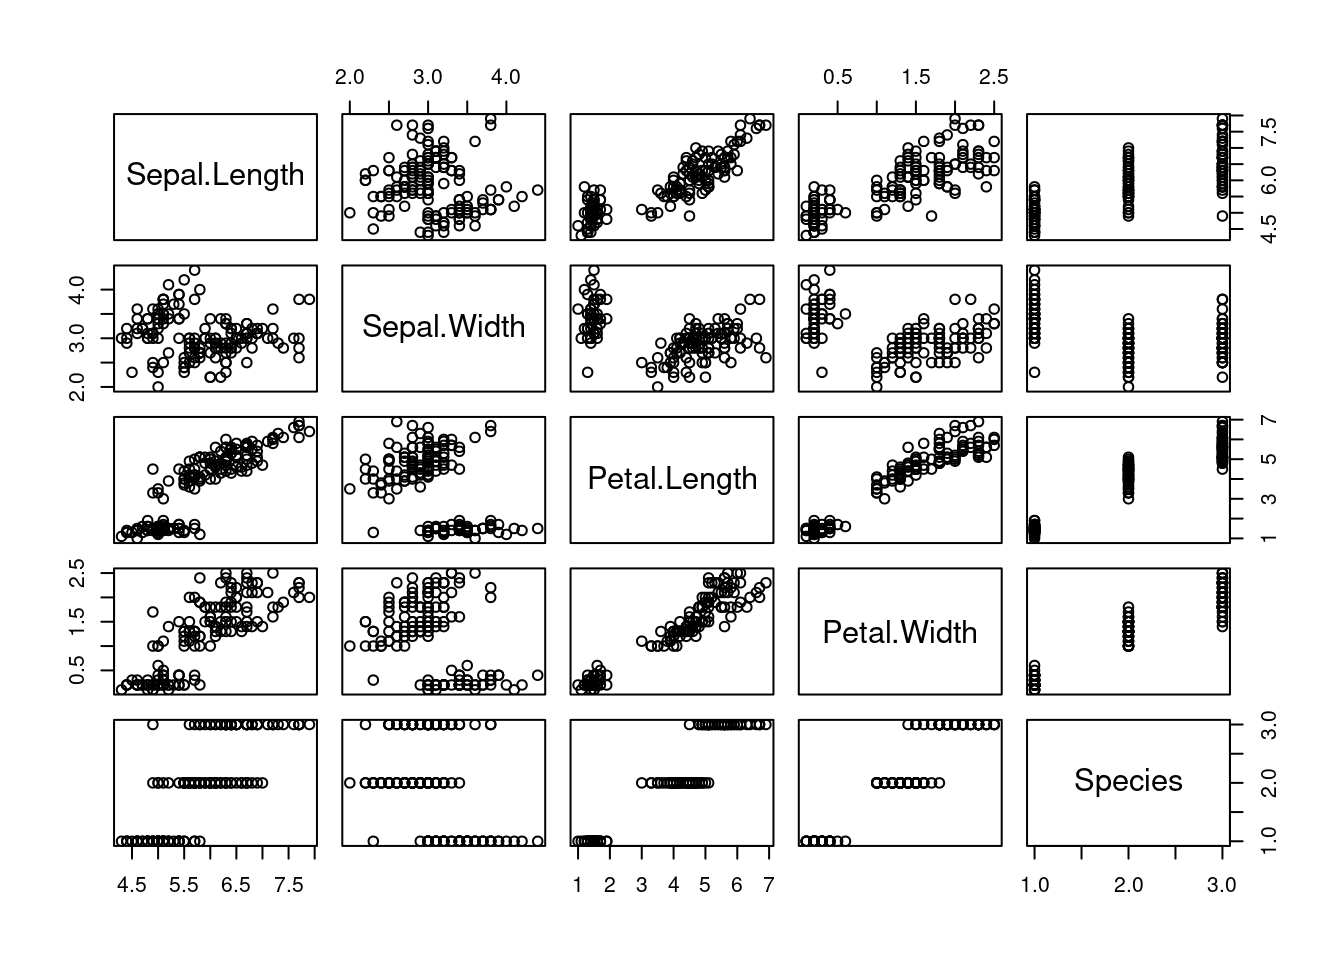
\includegraphics{bot89-introR_files/figure-latex/unnamed-chunk-238-1.pdf}

\begin{Shaded}
\begin{Highlighting}[]
\CommentTok{\# colocando todas com um único símbolo diferente}
\FunctionTok{plot}\NormalTok{(Sepalas, Petalas, }\AttributeTok{pch =} \DecValTok{25}\NormalTok{)}
\end{Highlighting}
\end{Shaded}

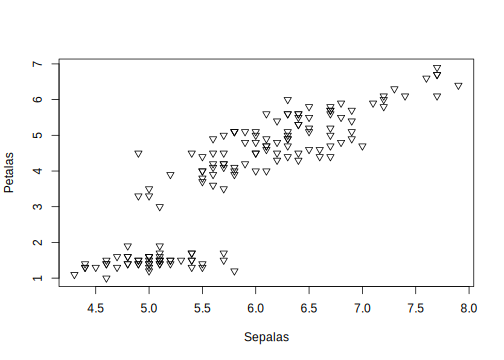
\includegraphics{bot89-introR_files/figure-latex/unnamed-chunk-238-2.pdf}

\begin{Shaded}
\begin{Highlighting}[]
\CommentTok{\# colocando cada espécie com um único símbolo}
\CommentTok{\# neste caso o argumento pch deve ter um vetor do número de linhas em iris, se for menor, pela regra da reciclagem, ele irá repetir os símbolo sem estar relacionado à coluna Species, que define qual linha é de qual espécie.}
\CommentTok{\# então se eu definir apenas três simbolos, um para cada espécie:}
\FunctionTok{plot}\NormalTok{(Sepalas, Petalas, }\AttributeTok{pch =} \FunctionTok{c}\NormalTok{(}\StringTok{"A"}\NormalTok{, }\StringTok{"\&"}\NormalTok{, }\StringTok{"+"}\NormalTok{))}
\end{Highlighting}
\end{Shaded}

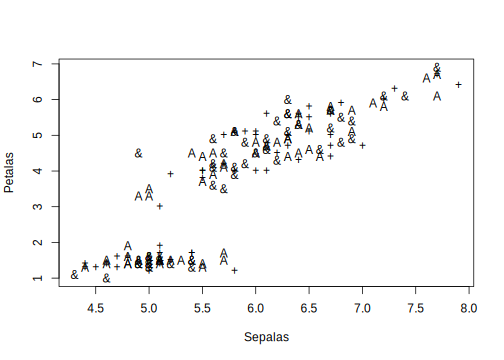
\includegraphics{bot89-introR_files/figure-latex/unnamed-chunk-238-3.pdf}

\begin{Shaded}
\begin{Highlighting}[]
\CommentTok{\# eles vao aparecer misturados, isso não está de acordo com as espécies}
\CommentTok{\# uma forma rápida de fazer isso, tendo em vista que o pch pode ser um valor numérico,}
\CommentTok{\# é transformar o nome das minhas especies em números.}
\CommentTok{\# Eu posso fazer isso se convertendo um fator para número, pois nele as categorias estão explicitamente definidas}
\NormalTok{spp }\OtherTok{\textless{}{-}}\NormalTok{ iris}\SpecialCharTok{$}\NormalTok{Species}
\FunctionTok{class}\NormalTok{(spp) }\CommentTok{\# já é um fator}
\end{Highlighting}
\end{Shaded}

\begin{verbatim}
## [1] "factor"
\end{verbatim}

\begin{Shaded}
\begin{Highlighting}[]
\CommentTok{\# note que isso gera muitos NAs, já vimos isso antes}
\FunctionTok{as.numeric}\NormalTok{(}\FunctionTok{as.vector}\NormalTok{(spp))}
\end{Highlighting}
\end{Shaded}

\begin{verbatim}
## Warning: NAs introduced by coercion
\end{verbatim}

\begin{verbatim}
##   [1] NA NA NA NA NA NA NA NA NA NA NA NA NA NA NA NA NA NA NA NA NA NA NA NA NA
##  [26] NA NA NA NA NA NA NA NA NA NA NA NA NA NA NA NA NA NA NA NA NA NA NA NA NA
##  [51] NA NA NA NA NA NA NA NA NA NA NA NA NA NA NA NA NA NA NA NA NA NA NA NA NA
##  [76] NA NA NA NA NA NA NA NA NA NA NA NA NA NA NA NA NA NA NA NA NA NA NA NA NA
## [101] NA NA NA NA NA NA NA NA NA NA NA NA NA NA NA NA NA NA NA NA NA NA NA NA NA
## [126] NA NA NA NA NA NA NA NA NA NA NA NA NA NA NA NA NA NA NA NA NA NA NA NA NA
\end{verbatim}

\begin{Shaded}
\begin{Highlighting}[]
\CommentTok{\# mas isso gera números por spp é um fator}
\FunctionTok{as.numeric}\NormalTok{(spp)}
\end{Highlighting}
\end{Shaded}

\begin{verbatim}
##   [1] 1 1 1 1 1 1 1 1 1 1 1 1 1 1 1 1 1 1 1 1 1 1 1 1 1 1 1 1 1 1 1 1 1 1 1 1 1
##  [38] 1 1 1 1 1 1 1 1 1 1 1 1 1 2 2 2 2 2 2 2 2 2 2 2 2 2 2 2 2 2 2 2 2 2 2 2 2
##  [75] 2 2 2 2 2 2 2 2 2 2 2 2 2 2 2 2 2 2 2 2 2 2 2 2 2 2 3 3 3 3 3 3 3 3 3 3 3
## [112] 3 3 3 3 3 3 3 3 3 3 3 3 3 3 3 3 3 3 3 3 3 3 3 3 3 3 3 3 3 3 3 3 3 3 3 3 3
## [149] 3 3
\end{verbatim}

\begin{Shaded}
\begin{Highlighting}[]
\CommentTok{\# então se eu quero os símbolos 22,23,25 para representar minhas espécies, eu uso esses números para pegar esses valores pelos índices de um vetor:}
\NormalTok{pch.das.spp }\OtherTok{\textless{}{-}} \FunctionTok{c}\NormalTok{(}\DecValTok{21}\NormalTok{, }\DecValTok{23}\NormalTok{, }\DecValTok{25}\NormalTok{)[}\FunctionTok{as.numeric}\NormalTok{(spp)]}
\NormalTok{pch.das.spp}
\end{Highlighting}
\end{Shaded}

\begin{verbatim}
##   [1] 21 21 21 21 21 21 21 21 21 21 21 21 21 21 21 21 21 21 21 21 21 21 21 21 21
##  [26] 21 21 21 21 21 21 21 21 21 21 21 21 21 21 21 21 21 21 21 21 21 21 21 21 21
##  [51] 23 23 23 23 23 23 23 23 23 23 23 23 23 23 23 23 23 23 23 23 23 23 23 23 23
##  [76] 23 23 23 23 23 23 23 23 23 23 23 23 23 23 23 23 23 23 23 23 23 23 23 23 23
## [101] 25 25 25 25 25 25 25 25 25 25 25 25 25 25 25 25 25 25 25 25 25 25 25 25 25
## [126] 25 25 25 25 25 25 25 25 25 25 25 25 25 25 25 25 25 25 25 25 25 25 25 25 25
\end{verbatim}

\begin{Shaded}
\begin{Highlighting}[]
\CommentTok{\# posso usar isso como argumento em plot:}
\FunctionTok{plot}\NormalTok{(Sepalas, Petalas, }\AttributeTok{pch =}\NormalTok{ pch.das.spp)}
\end{Highlighting}
\end{Shaded}

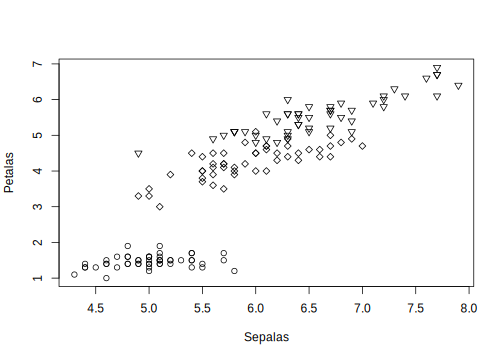
\includegraphics{bot89-introR_files/figure-latex/unnamed-chunk-238-4.pdf}

\begin{Shaded}
\begin{Highlighting}[]
\CommentTok{\# pronto cada espécie é um símbolo diferente}
\end{Highlighting}
\end{Shaded}

\subsection{\texorpdfstring{Tamanho dos pontos - \texttt{cex}}{Tamanho dos pontos - cex}}\label{tamanho-dos-pontos---cex}

O argumento genérico \texttt{cex} especifica o tamanho dos pontos relativo ao padrão do dispositivo.
Aceita um valor numérico que é multiplicado pelo valor do seu dispositivo.
O padrão geral é 1, isto é, 100\% do tamanho.
Se colocar 0.5 teremos 50\%; se 1.5, teremos 150\% do tamanho padrão.

\begin{Shaded}
\begin{Highlighting}[]
\CommentTok{\# da etapa anterior}
\NormalTok{pch.das.spp }\OtherTok{\textless{}{-}} \FunctionTok{c}\NormalTok{(}\DecValTok{21}\NormalTok{, }\DecValTok{23}\NormalTok{, }\DecValTok{25}\NormalTok{)[}\FunctionTok{as.numeric}\NormalTok{(spp)]}
\CommentTok{\# temos nosso gráfico com símbolos}
\FunctionTok{plot}\NormalTok{(Sepalas, Petalas, }\AttributeTok{pch =}\NormalTok{ pch.das.spp)}
\end{Highlighting}
\end{Shaded}

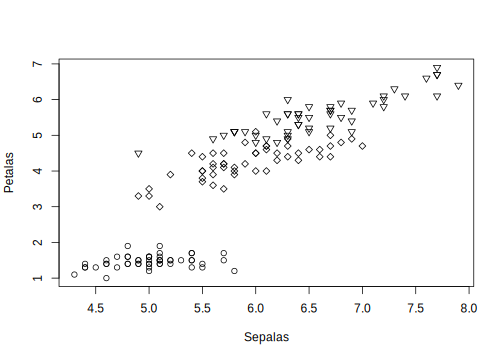
\includegraphics{bot89-introR_files/figure-latex/unnamed-chunk-239-1.pdf}

\begin{Shaded}
\begin{Highlighting}[]
\CommentTok{\# mudando o tamanho de todos os simbolos}
\FunctionTok{plot}\NormalTok{(Sepalas, Petalas, }\AttributeTok{pch =}\NormalTok{ pch.das.spp, }\AttributeTok{cex =} \FloatTok{0.5}\NormalTok{)}
\end{Highlighting}
\end{Shaded}

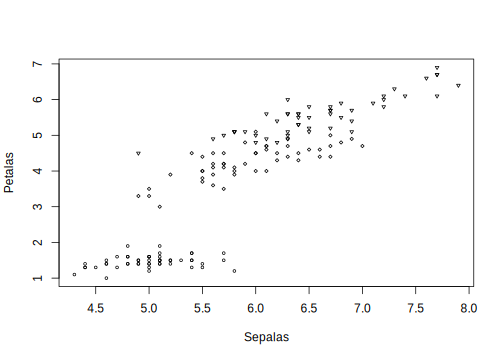
\includegraphics{bot89-introR_files/figure-latex/unnamed-chunk-239-2.pdf}

\begin{Shaded}
\begin{Highlighting}[]
\CommentTok{\# para maior}
\FunctionTok{plot}\NormalTok{(Sepalas, Petalas, }\AttributeTok{pch =}\NormalTok{ pch.das.spp, }\AttributeTok{cex =} \FloatTok{1.5}\NormalTok{)}
\end{Highlighting}
\end{Shaded}

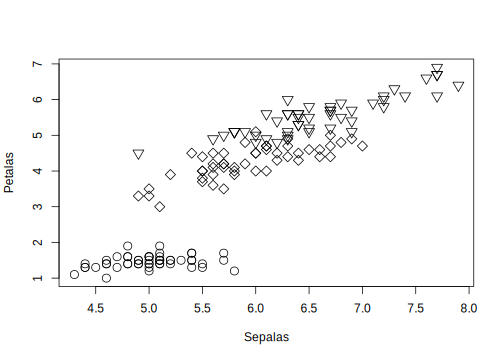
\includegraphics{bot89-introR_files/figure-latex/unnamed-chunk-239-3.pdf}

\begin{Shaded}
\begin{Highlighting}[]
\CommentTok{\# um tamanho diferente por ponto (especie)}
\NormalTok{tm }\OtherTok{\textless{}{-}} \FunctionTok{c}\NormalTok{(}\FloatTok{0.5}\NormalTok{, }\DecValTok{1}\NormalTok{, }\FloatTok{1.5}\NormalTok{)[}\FunctionTok{as.numeric}\NormalTok{(spp)]}
\NormalTok{tm}
\end{Highlighting}
\end{Shaded}

\begin{verbatim}
##   [1] 0.5 0.5 0.5 0.5 0.5 0.5 0.5 0.5 0.5 0.5 0.5 0.5 0.5 0.5 0.5 0.5 0.5 0.5
##  [19] 0.5 0.5 0.5 0.5 0.5 0.5 0.5 0.5 0.5 0.5 0.5 0.5 0.5 0.5 0.5 0.5 0.5 0.5
##  [37] 0.5 0.5 0.5 0.5 0.5 0.5 0.5 0.5 0.5 0.5 0.5 0.5 0.5 0.5 1.0 1.0 1.0 1.0
##  [55] 1.0 1.0 1.0 1.0 1.0 1.0 1.0 1.0 1.0 1.0 1.0 1.0 1.0 1.0 1.0 1.0 1.0 1.0
##  [73] 1.0 1.0 1.0 1.0 1.0 1.0 1.0 1.0 1.0 1.0 1.0 1.0 1.0 1.0 1.0 1.0 1.0 1.0
##  [91] 1.0 1.0 1.0 1.0 1.0 1.0 1.0 1.0 1.0 1.0 1.5 1.5 1.5 1.5 1.5 1.5 1.5 1.5
## [109] 1.5 1.5 1.5 1.5 1.5 1.5 1.5 1.5 1.5 1.5 1.5 1.5 1.5 1.5 1.5 1.5 1.5 1.5
## [127] 1.5 1.5 1.5 1.5 1.5 1.5 1.5 1.5 1.5 1.5 1.5 1.5 1.5 1.5 1.5 1.5 1.5 1.5
## [145] 1.5 1.5 1.5 1.5 1.5 1.5
\end{verbatim}

\begin{Shaded}
\begin{Highlighting}[]
\FunctionTok{plot}\NormalTok{(Sepalas, Petalas, }\AttributeTok{pch =}\NormalTok{ pch.das.spp, }\AttributeTok{cex =}\NormalTok{ tm)}
\end{Highlighting}
\end{Shaded}

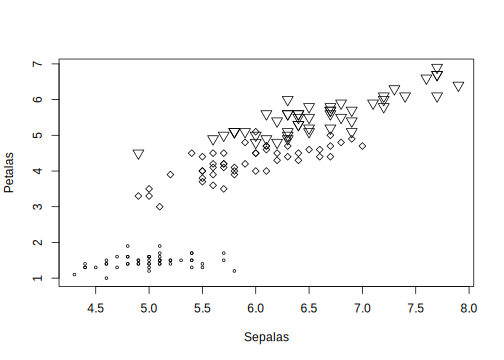
\includegraphics{bot89-introR_files/figure-latex/unnamed-chunk-239-4.pdf}

\subsection{Linhas}\label{linhas}

Os argumentos \texttt{lwd} e \texttt{lty} controlam a espessura e o tipo das linhas, respectivamente.

\begin{Shaded}
\begin{Highlighting}[]
\FunctionTok{data}\NormalTok{(}\StringTok{"AirPassengers"}\NormalTok{) }\CommentTok{\# veja esse conjunto de dados com ?datasets}
\FunctionTok{class}\NormalTok{(AirPassengers)}
\end{Highlighting}
\end{Shaded}

\begin{verbatim}
## [1] "ts"
\end{verbatim}

\begin{Shaded}
\begin{Highlighting}[]
\FunctionTok{plot}\NormalTok{(AirPassengers, }\AttributeTok{ylab =} \StringTok{"Número de Passageiros"}\NormalTok{)}
\end{Highlighting}
\end{Shaded}

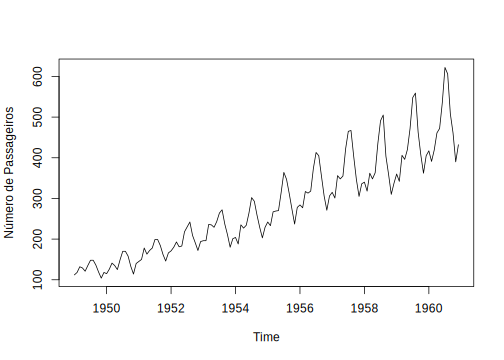
\includegraphics{bot89-introR_files/figure-latex/unnamed-chunk-240-1.pdf}

\begin{Shaded}
\begin{Highlighting}[]
\CommentTok{\# mudando o tipo de linha}
\FunctionTok{plot}\NormalTok{(AirPassengers, }\AttributeTok{ylab =} \StringTok{"Número de Passageiros"}\NormalTok{, }\AttributeTok{lty =} \StringTok{"dotted"}\NormalTok{)}
\end{Highlighting}
\end{Shaded}

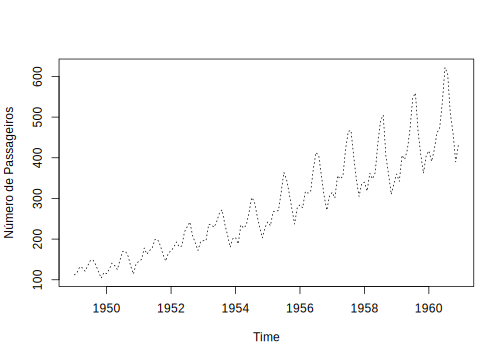
\includegraphics{bot89-introR_files/figure-latex/unnamed-chunk-240-2.pdf}

\begin{Shaded}
\begin{Highlighting}[]
\CommentTok{\# outro tipo}
\FunctionTok{plot}\NormalTok{(AirPassengers, }\AttributeTok{ylab =} \StringTok{"Número de Passageiros"}\NormalTok{, }\AttributeTok{lty =} \StringTok{"dotdash"}\NormalTok{)}
\end{Highlighting}
\end{Shaded}

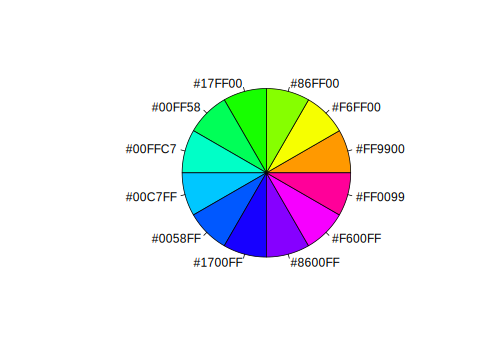
\includegraphics{bot89-introR_files/figure-latex/unnamed-chunk-240-3.pdf}

\begin{Shaded}
\begin{Highlighting}[]
\CommentTok{\# mudando a cor e espessura}
\FunctionTok{plot}\NormalTok{(AirPassengers, }\AttributeTok{ylab =} \StringTok{"Número de Passageiros"}\NormalTok{, }\AttributeTok{lty =} \StringTok{"dashed"}\NormalTok{, }\AttributeTok{col =} \StringTok{"red"}\NormalTok{, }\AttributeTok{lwd =} \DecValTok{2}\NormalTok{)}
\end{Highlighting}
\end{Shaded}

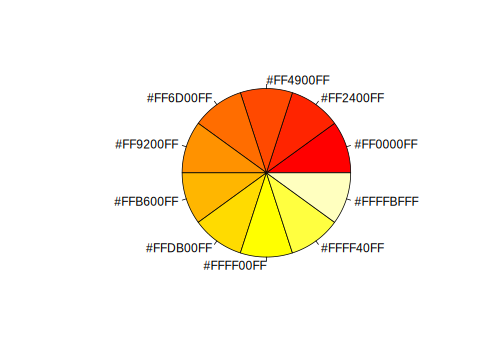
\includegraphics{bot89-introR_files/figure-latex/unnamed-chunk-240-4.pdf}

\subsection{\texorpdfstring{Cores de símbolos - \texttt{col} e \texttt{bg}}{Cores de símbolos - col e bg}}\label{cores-de-suxedmbolos---col-e-bg}

O argumento \texttt{col} define cores para os símbolos. No caso de símbolos de uma única cor, utilizamos apenas este argumento.
Já o argumento \texttt{bg} define as cores do preenchimento dos símbolos.

\begin{Shaded}
\begin{Highlighting}[]
\CommentTok{\# o que definimos antes são símbolos que permitem definir cores para preenchimento e linha:}
\NormalTok{pch.das.spp }\OtherTok{\textless{}{-}} \FunctionTok{c}\NormalTok{(}\DecValTok{21}\NormalTok{, }\DecValTok{23}\NormalTok{, }\DecValTok{25}\NormalTok{)[}\FunctionTok{as.numeric}\NormalTok{(spp)]}
\CommentTok{\# temos nosso gráfico com símbolos}
\FunctionTok{plot}\NormalTok{(Sepalas, Petalas, }\AttributeTok{pch =}\NormalTok{ pch.das.spp)}
\end{Highlighting}
\end{Shaded}

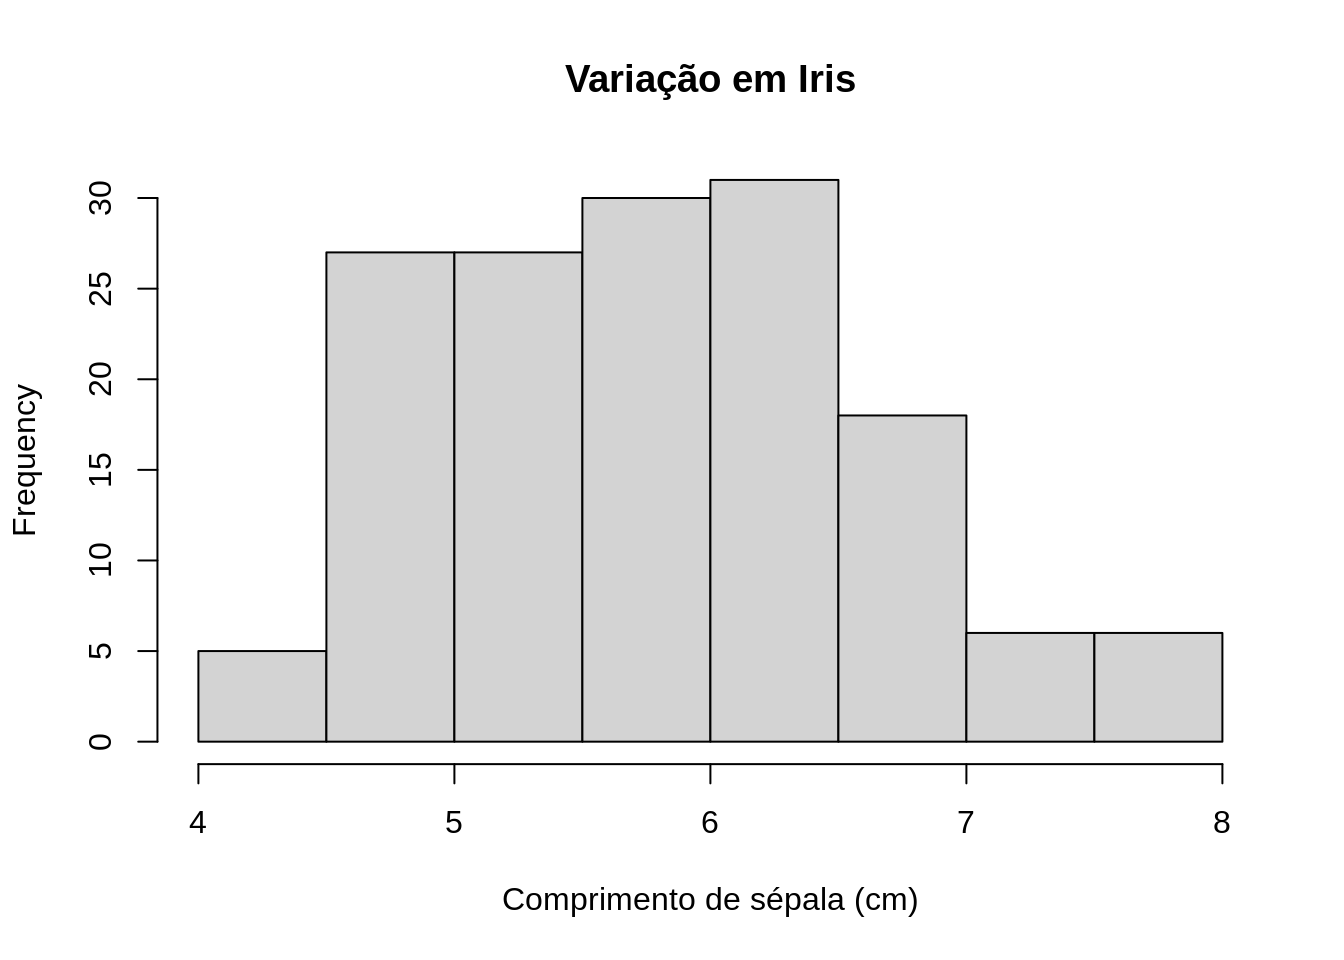
\includegraphics{bot89-introR_files/figure-latex/unnamed-chunk-241-1.pdf}

\begin{Shaded}
\begin{Highlighting}[]
\CommentTok{\# vamos adicionar as cores seguindo o mesmo raciocínio}
\NormalTok{cores.spp }\OtherTok{\textless{}{-}} \FunctionTok{c}\NormalTok{(}\StringTok{"red"}\NormalTok{, }\StringTok{"blue"}\NormalTok{, }\StringTok{"yellow"}\NormalTok{)[}\FunctionTok{as.numeric}\NormalTok{(spp)]}
\NormalTok{cores.spp}
\end{Highlighting}
\end{Shaded}

\begin{verbatim}
##   [1] "red"    "red"    "red"    "red"    "red"    "red"    "red"    "red"   
##   [9] "red"    "red"    "red"    "red"    "red"    "red"    "red"    "red"   
##  [17] "red"    "red"    "red"    "red"    "red"    "red"    "red"    "red"   
##  [25] "red"    "red"    "red"    "red"    "red"    "red"    "red"    "red"   
##  [33] "red"    "red"    "red"    "red"    "red"    "red"    "red"    "red"   
##  [41] "red"    "red"    "red"    "red"    "red"    "red"    "red"    "red"   
##  [49] "red"    "red"    "blue"   "blue"   "blue"   "blue"   "blue"   "blue"  
##  [57] "blue"   "blue"   "blue"   "blue"   "blue"   "blue"   "blue"   "blue"  
##  [65] "blue"   "blue"   "blue"   "blue"   "blue"   "blue"   "blue"   "blue"  
##  [73] "blue"   "blue"   "blue"   "blue"   "blue"   "blue"   "blue"   "blue"  
##  [81] "blue"   "blue"   "blue"   "blue"   "blue"   "blue"   "blue"   "blue"  
##  [89] "blue"   "blue"   "blue"   "blue"   "blue"   "blue"   "blue"   "blue"  
##  [97] "blue"   "blue"   "blue"   "blue"   "yellow" "yellow" "yellow" "yellow"
## [105] "yellow" "yellow" "yellow" "yellow" "yellow" "yellow" "yellow" "yellow"
## [113] "yellow" "yellow" "yellow" "yellow" "yellow" "yellow" "yellow" "yellow"
## [121] "yellow" "yellow" "yellow" "yellow" "yellow" "yellow" "yellow" "yellow"
## [129] "yellow" "yellow" "yellow" "yellow" "yellow" "yellow" "yellow" "yellow"
## [137] "yellow" "yellow" "yellow" "yellow" "yellow" "yellow" "yellow" "yellow"
## [145] "yellow" "yellow" "yellow" "yellow" "yellow" "yellow"
\end{verbatim}

\begin{Shaded}
\begin{Highlighting}[]
\FunctionTok{plot}\NormalTok{(Sepalas, Petalas, }\AttributeTok{pch =}\NormalTok{ pch.das.spp, }\AttributeTok{bg =}\NormalTok{ cores.spp)}
\end{Highlighting}
\end{Shaded}

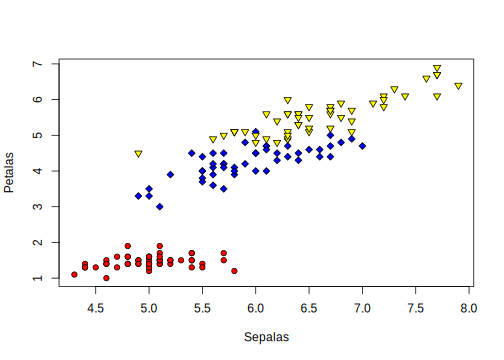
\includegraphics{bot89-introR_files/figure-latex/unnamed-chunk-241-2.pdf}

\begin{Shaded}
\begin{Highlighting}[]
\CommentTok{\# podemos mudar a cor da linha desses simbolos (todos para verde pela regra da reciclagem especifico uma única vez)}
\FunctionTok{plot}\NormalTok{(Sepalas, Petalas, }\AttributeTok{pch =}\NormalTok{ pch.das.spp, }\AttributeTok{bg =}\NormalTok{ cores.spp, }\AttributeTok{col =} \StringTok{"green"}\NormalTok{)}
\end{Highlighting}
\end{Shaded}

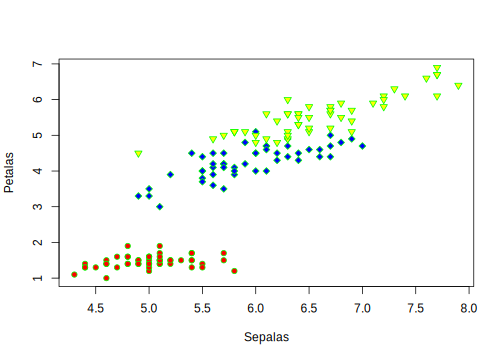
\includegraphics{bot89-introR_files/figure-latex/unnamed-chunk-241-3.pdf}

\begin{Shaded}
\begin{Highlighting}[]
\CommentTok{\# mudando simbolos}
\NormalTok{nsb }\OtherTok{\textless{}{-}} \FunctionTok{c}\NormalTok{(}\StringTok{"*"}\NormalTok{, }\StringTok{"\#"}\NormalTok{, }\StringTok{"+"}\NormalTok{)[}\FunctionTok{as.numeric}\NormalTok{(spp)]}
\FunctionTok{plot}\NormalTok{(Sepalas, Petalas, }\AttributeTok{pch =}\NormalTok{ nsb, }\AttributeTok{bg =}\NormalTok{ cores.spp)}
\end{Highlighting}
\end{Shaded}

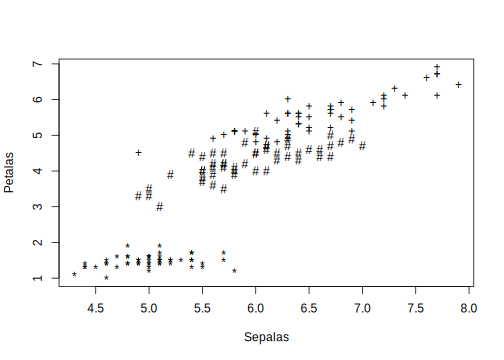
\includegraphics{bot89-introR_files/figure-latex/unnamed-chunk-241-4.pdf}

\begin{Shaded}
\begin{Highlighting}[]
\CommentTok{\# note que apesar de bg estar especificando cores as cores nao foram adicionadas, porque colocamos no argumento de preenchimento.}
\CommentTok{\# Mudando:}
\FunctionTok{plot}\NormalTok{(Sepalas, Petalas, }\AttributeTok{pch =}\NormalTok{ nsb, }\AttributeTok{col =}\NormalTok{ cores.spp)}
\end{Highlighting}
\end{Shaded}

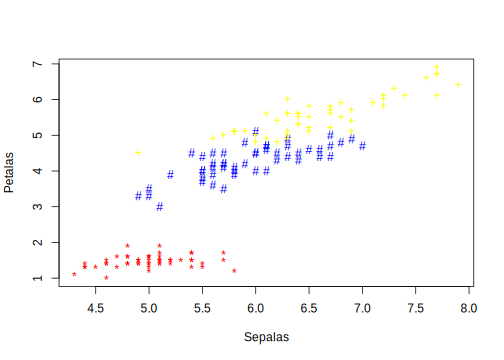
\includegraphics{bot89-introR_files/figure-latex/unnamed-chunk-241-5.pdf}

\subsection{Funções que definem cores}\label{funuxe7uxf5es-que-definem-cores}

Cores podem ser definidas por palavras ou por códigos.
As funções \texttt{colors()} ou \texttt{colours()} listam cores pelo nome.

\begin{Shaded}
\begin{Highlighting}[]
\CommentTok{\# lista todas as cores disponíveis pelo nome}
\FunctionTok{colors}\NormalTok{()}
\CommentTok{\# nossa tem 657 cores. Difícil, né?}
\CommentTok{\# reduz para as mais distintas}
\FunctionTok{colors}\NormalTok{(}\AttributeTok{distinct =} \ConstantTok{TRUE}\NormalTok{)}
\CommentTok{\# ainda 502}
\end{Highlighting}
\end{Shaded}

\begin{Shaded}
\begin{Highlighting}[]
\CommentTok{\# eu posso pegar ou buscar por cores}
\NormalTok{ascores }\OtherTok{\textless{}{-}} \FunctionTok{colors}\NormalTok{(}\AttributeTok{distinct =} \ConstantTok{TRUE}\NormalTok{)}
\NormalTok{vl }\OtherTok{\textless{}{-}} \FunctionTok{grep}\NormalTok{(}\StringTok{"blue"}\NormalTok{, ascores)}
\NormalTok{ascores[vl]}
\CommentTok{\# 60 nomes que contém a palavra azul}

\CommentTok{\# vamos ver todas as coresem umpdf longo}
\CommentTok{\# vamos plotar pizzas coloridas com 10 cores cada}
\CommentTok{\# 4 pizzas por página}
\end{Highlighting}
\end{Shaded}

\begin{Shaded}
\begin{Highlighting}[]
\NormalTok{?pie }\CommentTok{\# veja o help dessa função}
\end{Highlighting}
\end{Shaded}

\begin{Shaded}
\begin{Highlighting}[]
\CommentTok{\# abre um PDF}
\FunctionTok{pdf}\NormalTok{(}\StringTok{"cores.pdf"}\NormalTok{, }\AttributeTok{width =} \FunctionTok{lcm}\NormalTok{(}\DecValTok{29}\NormalTok{), }\AttributeTok{height =} \FunctionTok{lcm}\NormalTok{(}\DecValTok{21}\NormalTok{))}

\CommentTok{\# vamos dividir o dispositivo em 2 colunas e 3 linhas (e diminuir a margem)}
\FunctionTok{par}\NormalTok{(}\AttributeTok{mfrow =} \FunctionTok{c}\NormalTok{(}\DecValTok{2}\NormalTok{, }\DecValTok{2}\NormalTok{), }\AttributeTok{mar =} \FunctionTok{c}\NormalTok{(}\DecValTok{3}\NormalTok{, }\DecValTok{3}\NormalTok{, }\DecValTok{3}\NormalTok{, }\DecValTok{3}\NormalTok{), }\AttributeTok{cex =} \FloatTok{0.7}\NormalTok{)}
\NormalTok{ln }\OtherTok{\textless{}{-}} \FunctionTok{length}\NormalTok{(ascores)}
\NormalTok{ln }\CommentTok{\# sao 502 cores}
\FunctionTok{ceiling}\NormalTok{(ln }\SpecialCharTok{/} \DecValTok{10}\NormalTok{) }\CommentTok{\# , entao serao 51 pizzas}

\CommentTok{\# plota cada pizza fazendo uma iteração:}
\NormalTok{idx }\OtherTok{\textless{}{-}} \DecValTok{0} \CommentTok{\# o objeto nullo para usar de indice na iteracao para fazer de 10 em 10}
\ControlFlowTok{for}\NormalTok{ (p }\ControlFlowTok{in} \DecValTok{1}\SpecialCharTok{:}\FunctionTok{ceiling}\NormalTok{(ln }\SpecialCharTok{/} \DecValTok{10}\NormalTok{)) \{}
\NormalTok{  de }\OtherTok{\textless{}{-}}\NormalTok{ idx }\SpecialCharTok{+} \DecValTok{1} \CommentTok{\# cor do indice idx}
\NormalTok{  ate }\OtherTok{\textless{}{-}}\NormalTok{ idx }\SpecialCharTok{+} \DecValTok{10} \CommentTok{\# ate cor do indice idx+10}
\NormalTok{  cls }\OtherTok{\textless{}{-}}\NormalTok{ ascores[de}\SpecialCharTok{:}\NormalTok{ate] }\CommentTok{\# cores da pizza da iteracao p}
  \FunctionTok{pie}\NormalTok{(}\FunctionTok{rep}\NormalTok{(}\DecValTok{1}\NormalTok{, }\DecValTok{10}\NormalTok{), }\AttributeTok{col =}\NormalTok{ cls, }\AttributeTok{labels =}\NormalTok{ cls)}
\NormalTok{  idx }\OtherTok{\textless{}{-}}\NormalTok{ ate}
\NormalTok{\}}
\FunctionTok{dev.off}\NormalTok{() }\CommentTok{\# fecha o pdf}
\end{Highlighting}
\end{Shaded}

As funções \texttt{rainbow()} ou \texttt{terrain.colors()} geram gradientes de cores em um padrão definido.

\begin{Shaded}
\begin{Highlighting}[]
\CommentTok{\# 10 cores do arco{-}iris}
\NormalTok{cls }\OtherTok{\textless{}{-}} \FunctionTok{rainbow}\NormalTok{(}\AttributeTok{n =} \DecValTok{10}\NormalTok{)}
\FunctionTok{pie}\NormalTok{(}\FunctionTok{rep}\NormalTok{(}\DecValTok{1}\NormalTok{, }\DecValTok{10}\NormalTok{), }\AttributeTok{col =}\NormalTok{ cls, }\AttributeTok{labels =}\NormalTok{ cls)}
\end{Highlighting}
\end{Shaded}

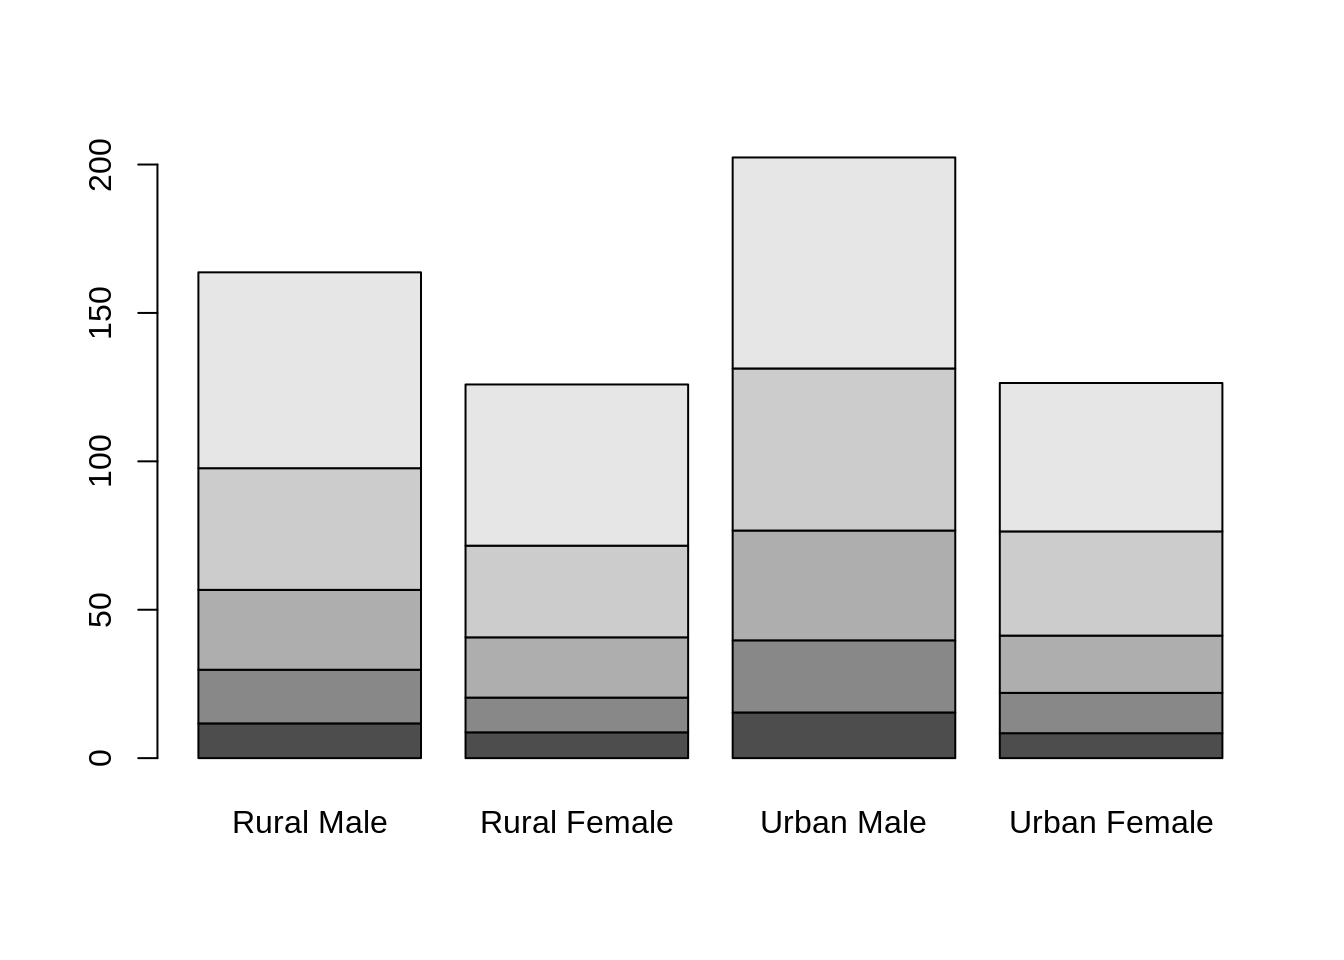
\includegraphics{bot89-introR_files/figure-latex/unnamed-chunk-246-1.pdf}

\begin{Shaded}
\begin{Highlighting}[]
\CommentTok{\# 12 cores do arco{-}iris com 50\% de transparencia}
\NormalTok{cls }\OtherTok{\textless{}{-}} \FunctionTok{rainbow}\NormalTok{(}\AttributeTok{n =} \DecValTok{12}\NormalTok{, }\AttributeTok{alpha =} \FloatTok{0.5}\NormalTok{)}
\FunctionTok{pie}\NormalTok{(}\FunctionTok{rep}\NormalTok{(}\DecValTok{1}\NormalTok{, }\DecValTok{12}\NormalTok{), }\AttributeTok{col =}\NormalTok{ cls, }\AttributeTok{labels =}\NormalTok{ cls)}
\end{Highlighting}
\end{Shaded}

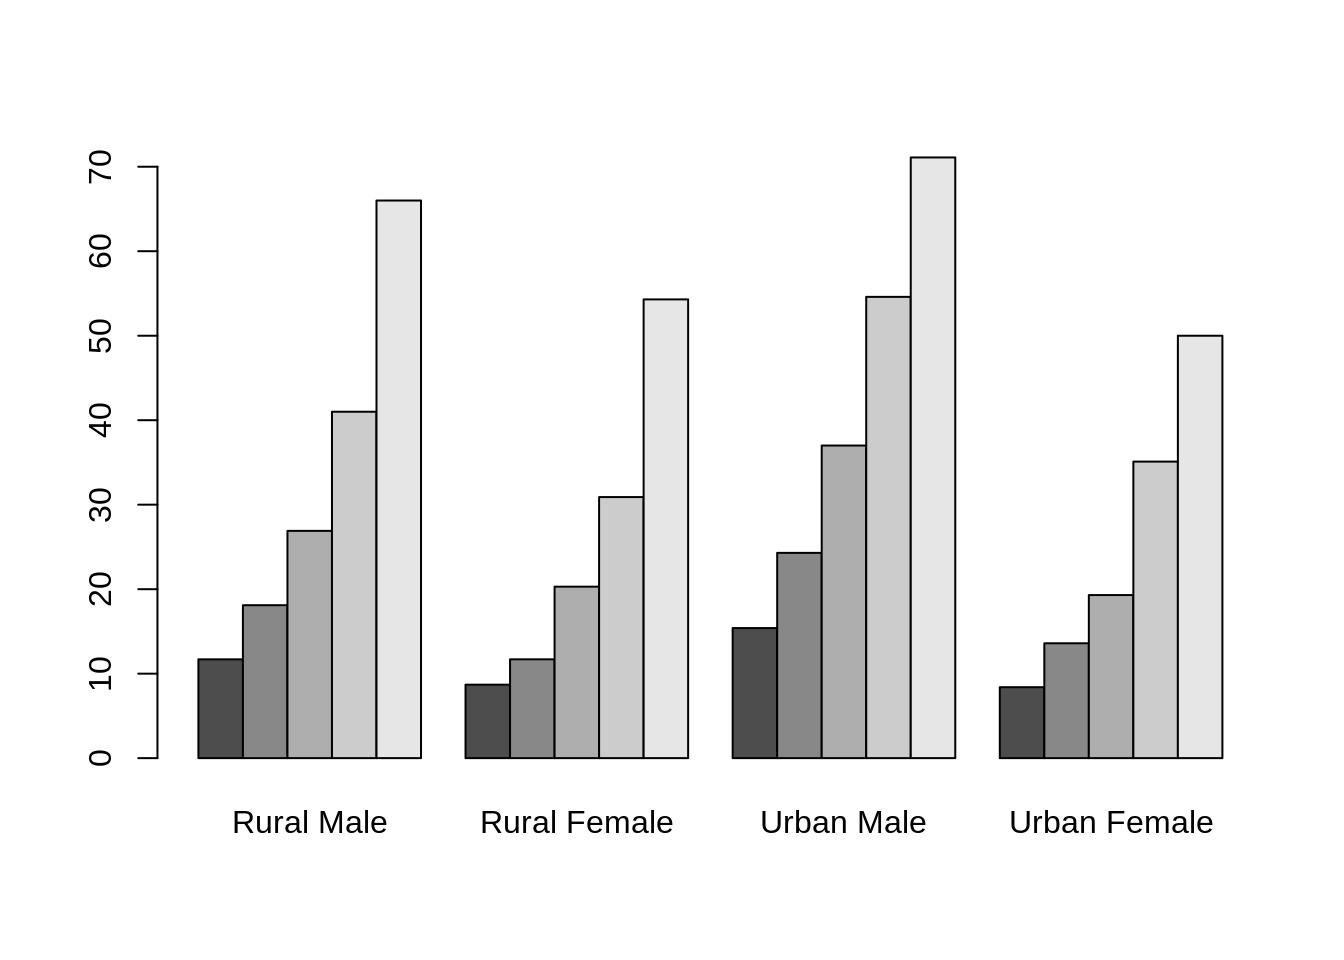
\includegraphics{bot89-introR_files/figure-latex/unnamed-chunk-246-2.pdf}

\begin{Shaded}
\begin{Highlighting}[]
\CommentTok{\# 12 cores do arco{-}iris, limitando o espectro}
\NormalTok{cls }\OtherTok{\textless{}{-}} \FunctionTok{rainbow}\NormalTok{(}\AttributeTok{n =} \DecValTok{12}\NormalTok{, }\AttributeTok{start =} \FloatTok{0.1}\NormalTok{, }\AttributeTok{end =} \FloatTok{0.9}\NormalTok{)}
\FunctionTok{pie}\NormalTok{(}\FunctionTok{rep}\NormalTok{(}\DecValTok{1}\NormalTok{, }\DecValTok{12}\NormalTok{), }\AttributeTok{col =}\NormalTok{ cls, }\AttributeTok{labels =}\NormalTok{ cls)}
\end{Highlighting}
\end{Shaded}

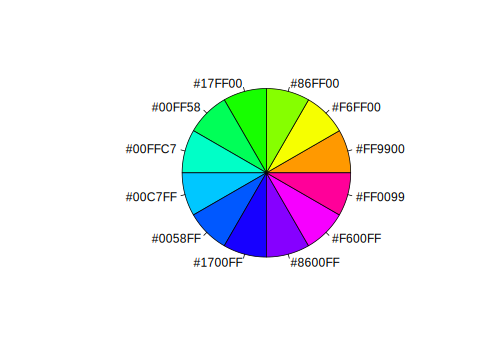
\includegraphics{bot89-introR_files/figure-latex/unnamed-chunk-246-3.pdf}

\begin{Shaded}
\begin{Highlighting}[]
\CommentTok{\# 10 cores quentes}
\NormalTok{cls }\OtherTok{\textless{}{-}} \FunctionTok{heat.colors}\NormalTok{(}\AttributeTok{n =} \DecValTok{10}\NormalTok{, }\AttributeTok{alpha =} \DecValTok{1}\NormalTok{)}
\FunctionTok{pie}\NormalTok{(}\FunctionTok{rep}\NormalTok{(}\DecValTok{1}\NormalTok{, }\DecValTok{10}\NormalTok{), }\AttributeTok{col =}\NormalTok{ cls, }\AttributeTok{labels =}\NormalTok{ cls)}
\end{Highlighting}
\end{Shaded}

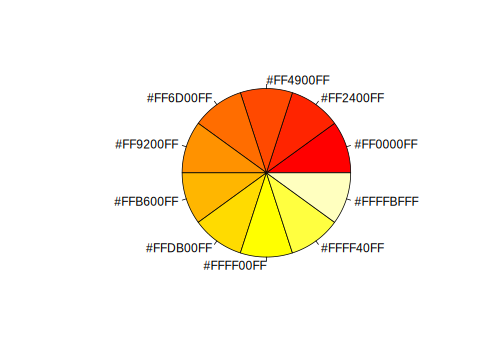
\includegraphics{bot89-introR_files/figure-latex/unnamed-chunk-246-4.pdf}

\begin{Shaded}
\begin{Highlighting}[]
\CommentTok{\# 20 cores topográficas}
\NormalTok{cls }\OtherTok{\textless{}{-}} \FunctionTok{topo.colors}\NormalTok{(}\AttributeTok{n =} \DecValTok{20}\NormalTok{, }\AttributeTok{alpha =} \DecValTok{1}\NormalTok{)}
\FunctionTok{pie}\NormalTok{(}\FunctionTok{rep}\NormalTok{(}\DecValTok{1}\NormalTok{, }\DecValTok{20}\NormalTok{), }\AttributeTok{col =}\NormalTok{ cls, }\AttributeTok{labels =}\NormalTok{ cls)}
\end{Highlighting}
\end{Shaded}

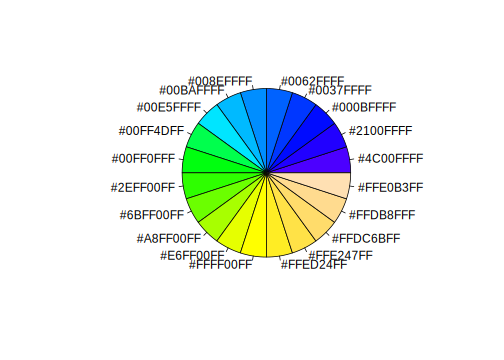
\includegraphics{bot89-introR_files/figure-latex/unnamed-chunk-246-5.pdf}

\begin{Shaded}
\begin{Highlighting}[]
\CommentTok{\# ou melhor}
\NormalTok{cls }\OtherTok{\textless{}{-}} \FunctionTok{terrain.colors}\NormalTok{(}\AttributeTok{n =} \DecValTok{20}\NormalTok{, }\AttributeTok{alpha =} \DecValTok{1}\NormalTok{)}
\FunctionTok{pie}\NormalTok{(}\FunctionTok{rep}\NormalTok{(}\DecValTok{1}\NormalTok{, }\DecValTok{20}\NormalTok{), }\AttributeTok{col =}\NormalTok{ cls, }\AttributeTok{labels =}\NormalTok{ cls)}
\end{Highlighting}
\end{Shaded}

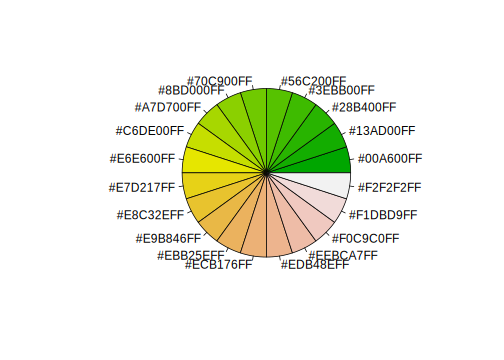
\includegraphics{bot89-introR_files/figure-latex/unnamed-chunk-246-6.pdf}

As funções \texttt{rgb()} ou \texttt{hsv()} geram qualquer tipo de cor para ser utilizados nos gráficos.

\begin{Shaded}
\begin{Highlighting}[]
\NormalTok{?rgb }\CommentTok{\# veja o help dessa funcao e veja as funcoes sob See Also}
\end{Highlighting}
\end{Shaded}

\begin{Shaded}
\begin{Highlighting}[]
\CommentTok{\# podemos entender melhor fazendo o caminho inverso}
\NormalTok{defs }\OtherTok{\textless{}{-}} \FunctionTok{col2rgb}\NormalTok{(}\StringTok{"yellow"}\NormalTok{) }\CommentTok{\# extraimos as especificacoes de amarelo (cores primárias ) pela palavra}
\NormalTok{defs}
\end{Highlighting}
\end{Shaded}

\begin{tabular}{l|r}
\hline
red & 255\\
\hline
green & 255\\
\hline
blue & 0\\
\hline
\end{tabular}

\begin{Shaded}
\begin{Highlighting}[]
\CommentTok{\# sem cor temos preto}
\NormalTok{cls }\OtherTok{\textless{}{-}} \FunctionTok{rgb}\NormalTok{(}\AttributeTok{red =} \DecValTok{0}\NormalTok{, }\AttributeTok{green =} \DecValTok{0}\NormalTok{, }\AttributeTok{blue =} \DecValTok{0}\NormalTok{) }\CommentTok{\# fazemos amarelo}
\FunctionTok{pie}\NormalTok{(}\DecValTok{1}\NormalTok{, }\AttributeTok{col =}\NormalTok{ cls, }\AttributeTok{labels =}\NormalTok{ cls)}
\end{Highlighting}
\end{Shaded}

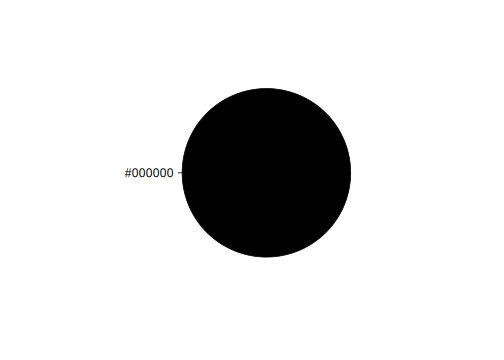
\includegraphics{bot89-introR_files/figure-latex/unnamed-chunk-248-1.pdf}

\begin{Shaded}
\begin{Highlighting}[]
\CommentTok{\# fazemos amarelo}
\NormalTok{cls }\OtherTok{\textless{}{-}} \FunctionTok{rgb}\NormalTok{(}\AttributeTok{red =} \DecValTok{255}\NormalTok{, }\AttributeTok{green =} \DecValTok{255}\NormalTok{, }\AttributeTok{blue =} \DecValTok{0}\NormalTok{, }\AttributeTok{maxColorValue =} \DecValTok{255}\NormalTok{)}
\FunctionTok{pie}\NormalTok{(}\DecValTok{1}\NormalTok{, }\AttributeTok{col =}\NormalTok{ cls, }\AttributeTok{labels =}\NormalTok{ cls)}
\end{Highlighting}
\end{Shaded}

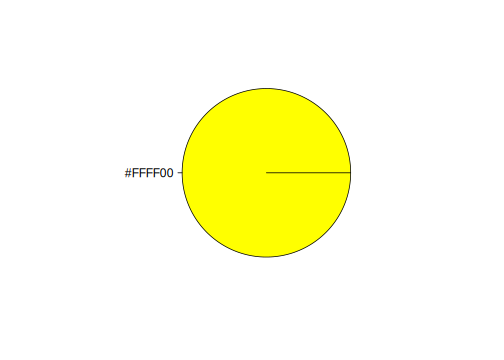
\includegraphics{bot89-introR_files/figure-latex/unnamed-chunk-248-2.pdf}

\begin{Shaded}
\begin{Highlighting}[]
\CommentTok{\# tiramos verde}
\NormalTok{cls }\OtherTok{\textless{}{-}} \FunctionTok{rgb}\NormalTok{(}\AttributeTok{red =} \DecValTok{255}\NormalTok{, }\AttributeTok{green =} \DecValTok{160}\NormalTok{, }\AttributeTok{blue =} \DecValTok{0}\NormalTok{, }\AttributeTok{maxColorValue =} \DecValTok{255}\NormalTok{)}
\FunctionTok{pie}\NormalTok{(}\DecValTok{1}\NormalTok{, }\AttributeTok{col =}\NormalTok{ cls, }\AttributeTok{labels =}\NormalTok{ cls)}
\end{Highlighting}
\end{Shaded}

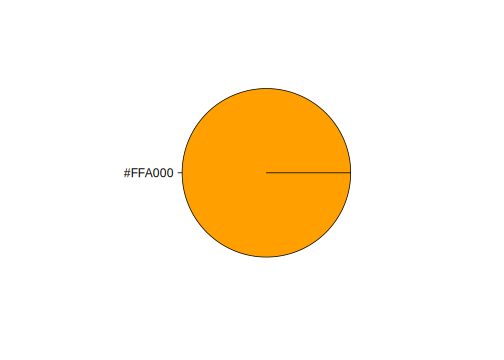
\includegraphics{bot89-introR_files/figure-latex/unnamed-chunk-248-3.pdf}

\begin{Shaded}
\begin{Highlighting}[]
\CommentTok{\# tiramos verde e adicionamos azul}
\NormalTok{cls }\OtherTok{\textless{}{-}} \FunctionTok{rgb}\NormalTok{(}\AttributeTok{red =} \DecValTok{255}\NormalTok{, }\AttributeTok{green =} \DecValTok{160}\NormalTok{, }\AttributeTok{blue =} \DecValTok{255}\NormalTok{, }\AttributeTok{maxColorValue =} \DecValTok{255}\NormalTok{)}
\FunctionTok{pie}\NormalTok{(}\DecValTok{1}\NormalTok{, }\AttributeTok{col =}\NormalTok{ cls, }\AttributeTok{labels =}\NormalTok{ cls)}
\end{Highlighting}
\end{Shaded}

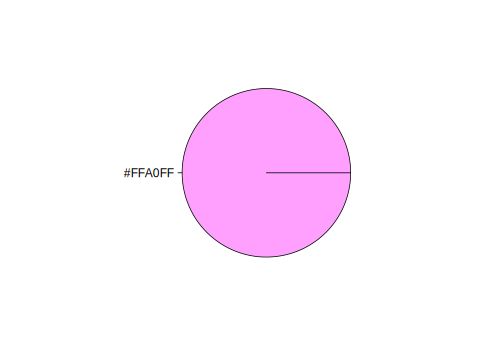
\includegraphics{bot89-introR_files/figure-latex/unnamed-chunk-248-4.pdf}

\begin{Shaded}
\begin{Highlighting}[]
\CommentTok{\# tiramos azul{-}escuro (mais perto de 0)}
\NormalTok{cls }\OtherTok{\textless{}{-}} \FunctionTok{rgb}\NormalTok{(}\AttributeTok{red =} \DecValTok{0}\NormalTok{, }\AttributeTok{green =} \DecValTok{0}\NormalTok{, }\AttributeTok{blue =} \DecValTok{150}\NormalTok{, }\AttributeTok{maxColorValue =} \DecValTok{255}\NormalTok{)}
\FunctionTok{pie}\NormalTok{(}\DecValTok{1}\NormalTok{, }\AttributeTok{col =}\NormalTok{ cls, }\AttributeTok{labels =}\NormalTok{ cls)}
\end{Highlighting}
\end{Shaded}

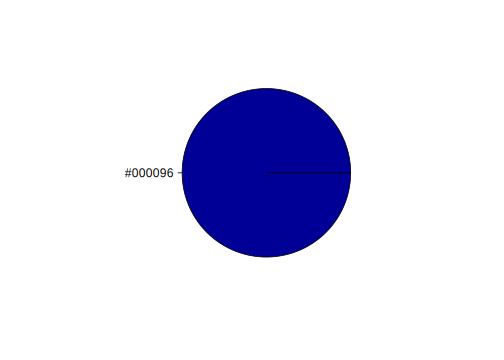
\includegraphics{bot89-introR_files/figure-latex/unnamed-chunk-248-5.pdf}

\begin{Shaded}
\begin{Highlighting}[]
\CommentTok{\# tiramos azul}
\NormalTok{cls }\OtherTok{\textless{}{-}} \FunctionTok{rgb}\NormalTok{(}\AttributeTok{red =} \DecValTok{0}\NormalTok{, }\AttributeTok{green =} \DecValTok{0}\NormalTok{, }\AttributeTok{blue =} \DecValTok{255}\NormalTok{, }\AttributeTok{maxColorValue =} \DecValTok{255}\NormalTok{)}
\FunctionTok{pie}\NormalTok{(}\DecValTok{1}\NormalTok{, }\AttributeTok{col =}\NormalTok{ cls, }\AttributeTok{labels =}\NormalTok{ cls)}
\end{Highlighting}
\end{Shaded}

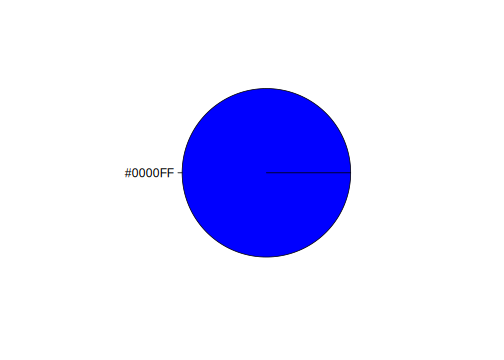
\includegraphics{bot89-introR_files/figure-latex/unnamed-chunk-248-6.pdf}

\section{Funções gráficas de alto nível}\label{graf-alto-nivel}

Funções gráficas de alto-nível (\emph{highlevel plots}) são as funções que usamos para gerar os gráficos.
Além da função genérica \texttt{plot()}, veremos apenas alguns poucos exemplos, mas existem diversas funções gráficas de alto nível, muitas das quais dependem de pacotes específicos.
Existem inúmeras outras funções de alto-nível, algumas do R-base, outras geradas por colaboradores na forma de \href{https://cran.r-project.org/web/packages/}{pacotes do R}.
A função \texttt{plot()} entende algumas dessas outras funções dos pacotes automaticamente, dependendo da classe do objeto, e você sequer precisa usar o nome específico (veja o exemplo em plot.phylo(), abaixo).

No \texttt{?} do pacote graphics, você encontra ajuda para funções gráficas em geral:

\begin{Shaded}
\begin{Highlighting}[]
\FunctionTok{demo}\NormalTok{(}\StringTok{"graphics"}\NormalTok{) }\CommentTok{\# execute este demostrativo {-} lembre{-}se de interagir no console do R para as figuras}
\NormalTok{?graphics }\CommentTok{\# veja o help dessa função para alguns gráficos}
\end{Highlighting}
\end{Shaded}

\subsection{\texorpdfstring{\texttt{plot()} - uma função genérica}{plot() - uma função genérica}}\label{plot---uma-funuxe7uxe3o-genuxe9rica}

A função \texttt{plot()} é a principal para produção de gráficos porque é uma \textbf{função genérica} que irá gerar um gráfico dependendo da \hyperref[classes]{classe do objeto}. Em muitos casos, não precisamos usar outras funções, porque a depender da classe do objeto, esta função automaticamente entenderá o que você precisa.

\begin{Shaded}
\begin{Highlighting}[]
\NormalTok{?plot }\CommentTok{\# veja o help dessa função}
\end{Highlighting}
\end{Shaded}

Suponha que tenhamos um vetor simples e numérico chamado \texttt{vv}:

\begin{Shaded}
\begin{Highlighting}[]
\NormalTok{vv }\OtherTok{\textless{}{-}} \DecValTok{1}\SpecialCharTok{:}\DecValTok{10}
\CommentTok{\# Qual e a classe desse vetor?}
\FunctionTok{class}\NormalTok{(vv)}
\end{Highlighting}
\end{Shaded}

\begin{verbatim}
## [1] "integer"
\end{verbatim}

Vamos plotá-lo:

\begin{Shaded}
\begin{Highlighting}[]
\FunctionTok{plot}\NormalTok{(vv)}
\end{Highlighting}
\end{Shaded}

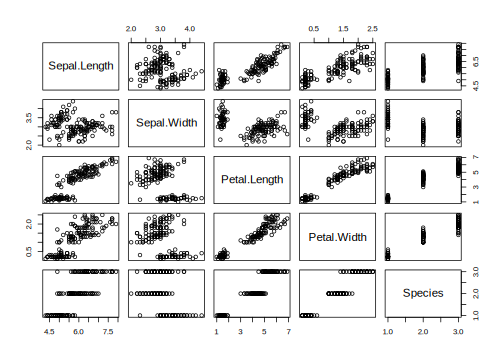
\includegraphics{bot89-introR_files/figure-latex/unnamed-chunk-252-1.pdf}

Vamos mudar alguns argumentos da função \texttt{plot()}.
Acrescentaremos um tipo diferente de ponto (argumento \texttt{pch}), uma cor vermelha para o fundo do ponto (argumento \texttt{bg}), um novo texto para o eixo x (argumento \texttt{xlab}), um novo texto para o eixo y (argumento \texttt{ylab}), e um título para o plot (argumento \texttt{main}):

\begin{Shaded}
\begin{Highlighting}[]
\FunctionTok{plot}\NormalTok{(vv, }\AttributeTok{pch =} \DecValTok{21}\NormalTok{, }\AttributeTok{bg =} \StringTok{"red"}\NormalTok{, }\AttributeTok{xlab =} \StringTok{"índice do vetor"}\NormalTok{, }\AttributeTok{ylab =} \StringTok{"valor do vetor"}\NormalTok{, }\AttributeTok{main =} \StringTok{"Plotando um vetor"}\NormalTok{)}
\end{Highlighting}
\end{Shaded}

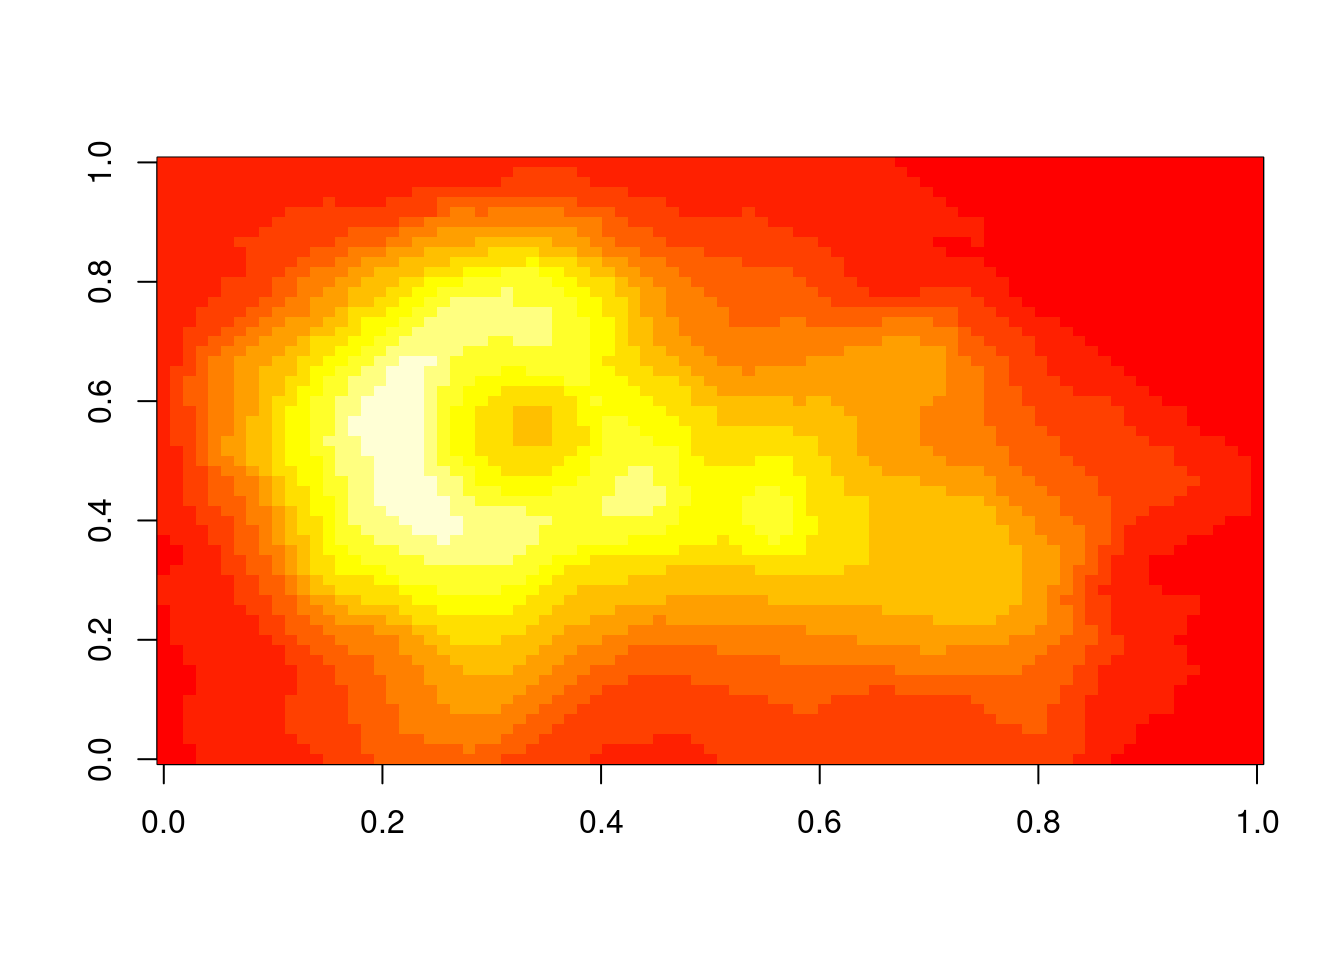
\includegraphics{bot89-introR_files/figure-latex/unnamed-chunk-253-1.pdf}

Vamos trabalhar agora com uma matriz de duas colunas:

\begin{Shaded}
\begin{Highlighting}[]
\NormalTok{xx }\OtherTok{\textless{}{-}} \DecValTok{1}\SpecialCharTok{:}\DecValTok{10} \CommentTok{\# um vetor}
\NormalTok{yy }\OtherTok{\textless{}{-}} \DecValTok{10}\SpecialCharTok{:}\DecValTok{1} \CommentTok{\# o mesmo vetor invertido}
\NormalTok{mm }\OtherTok{\textless{}{-}} \FunctionTok{cbind}\NormalTok{(xx, yy) }\CommentTok{\# junta em uma matrix}
\CommentTok{\# Qual a classe dessa matriz?}
\FunctionTok{class}\NormalTok{(mm)}
\end{Highlighting}
\end{Shaded}

\begin{verbatim}
## [1] "matrix" "array"
\end{verbatim}

Vamos utilizar a matriz de duas colunas \texttt{mm} diretamente como primeiro argumento da função \texttt{plot()}:

\begin{Shaded}
\begin{Highlighting}[]
\FunctionTok{plot}\NormalTok{(mm, }\AttributeTok{xlab =} \StringTok{"Eixo X"}\NormalTok{, }\AttributeTok{ylab =} \StringTok{"Eixo Y"}\NormalTok{, }\AttributeTok{main =} \StringTok{"Plotando uma matriz de 2 colunas"}\NormalTok{)}
\end{Highlighting}
\end{Shaded}

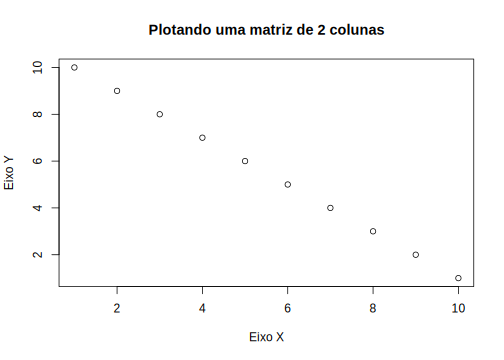
\includegraphics{bot89-introR_files/figure-latex/unnamed-chunk-255-1.pdf}

Podemos também especificar separadamente os eixos x e y, utilizando os vetores \texttt{xx} e \texttt{yy}, utilizados para compor a matriz \texttt{mm}:

\begin{Shaded}
\begin{Highlighting}[]
\CommentTok{\# ou poderia especificar diretamente os eixos xx e yy sem usar a matriz}
\FunctionTok{plot}\NormalTok{(xx, yy, }\AttributeTok{xlab =} \StringTok{"Eixo X"}\NormalTok{, }\AttributeTok{ylab =} \StringTok{"Eixo Y"}\NormalTok{, }\AttributeTok{main =} \StringTok{"Plotando uma matriz de 2 colunas"}\NormalTok{, }\AttributeTok{pch =} \DecValTok{21}\NormalTok{, }\AttributeTok{bg =} \StringTok{"purple"}\NormalTok{)}
\end{Highlighting}
\end{Shaded}

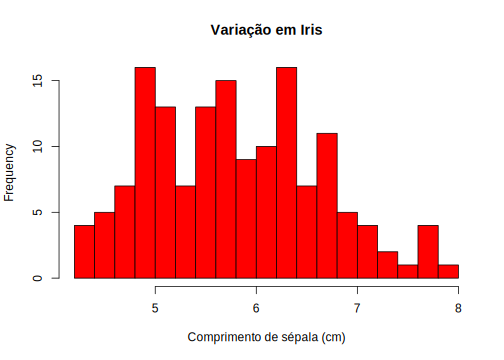
\includegraphics{bot89-introR_files/figure-latex/unnamed-chunk-256-1.pdf}

Se temos um conjunto de dados e queremos ver a relação entre si de todas as colunas do conjunto, podemos simplesmente usar:

\begin{Shaded}
\begin{Highlighting}[]
\FunctionTok{class}\NormalTok{(iris) }\CommentTok{\# um conjunto de dados no formato data.frame}
\end{Highlighting}
\end{Shaded}

\begin{verbatim}
## [1] "data.frame"
\end{verbatim}

\begin{Shaded}
\begin{Highlighting}[]
\FunctionTok{plot}\NormalTok{(iris)}
\end{Highlighting}
\end{Shaded}

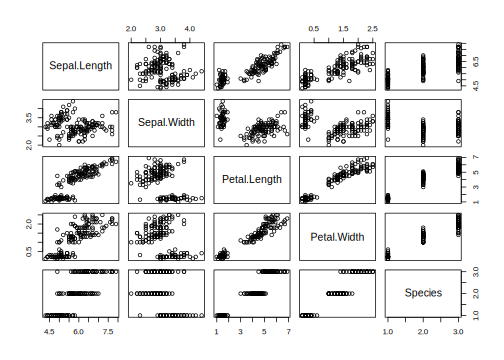
\includegraphics{bot89-introR_files/figure-latex/unnamed-chunk-258-1.pdf}

\begin{Shaded}
\begin{Highlighting}[]
\CommentTok{\# o nome dos eixos está na diagonal dessa figura}
\end{Highlighting}
\end{Shaded}

\subsection{\texorpdfstring{\texttt{hist()}}{hist()}}\label{hist}

Esta importante função serve para visualizar a variação de uma variável apenas.

\begin{Shaded}
\begin{Highlighting}[]
\NormalTok{?hist }\CommentTok{\# veja o help}
\end{Highlighting}
\end{Shaded}

Vamos utilizar apenas a variável \texttt{Sepal.Length} do conjunto de dados \texttt{iris}:

\begin{Shaded}
\begin{Highlighting}[]
\FunctionTok{class}\NormalTok{(iris}\SpecialCharTok{$}\NormalTok{Sepal.Length) }\CommentTok{\# é um vetor}
\end{Highlighting}
\end{Shaded}

\begin{verbatim}
## [1] "numeric"
\end{verbatim}

\begin{Shaded}
\begin{Highlighting}[]
\FunctionTok{hist}\NormalTok{(iris}\SpecialCharTok{$}\NormalTok{Sepal.Length, }\AttributeTok{xlab =} \StringTok{"Comprimento de sépala (cm)"}\NormalTok{, }\AttributeTok{main =} \StringTok{"Variação em Iris"}\NormalTok{)}
\end{Highlighting}
\end{Shaded}

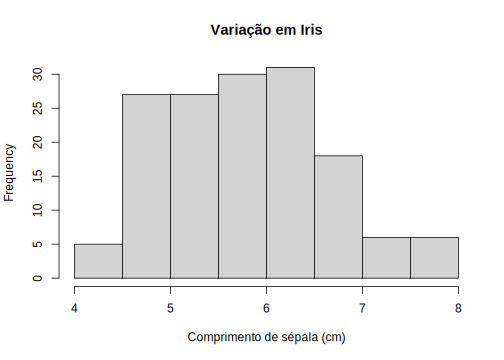
\includegraphics{bot89-introR_files/figure-latex/unnamed-chunk-261-1.pdf}
Vamos diminuir os espaçamentos entre as barras e colorí-las:

\begin{Shaded}
\begin{Highlighting}[]
\CommentTok{\# diminuindo os espaçamentos entre as barras e colorindo}
\FunctionTok{hist}\NormalTok{(iris}\SpecialCharTok{$}\NormalTok{Sepal.Length, }\AttributeTok{xlab =} \StringTok{"Comprimento de sépala (cm)"}\NormalTok{, }\AttributeTok{main =} \StringTok{"Variação em Iris"}\NormalTok{, }\AttributeTok{breaks =} \DecValTok{20}\NormalTok{, }\AttributeTok{col =} \StringTok{"red"}\NormalTok{)}
\end{Highlighting}
\end{Shaded}

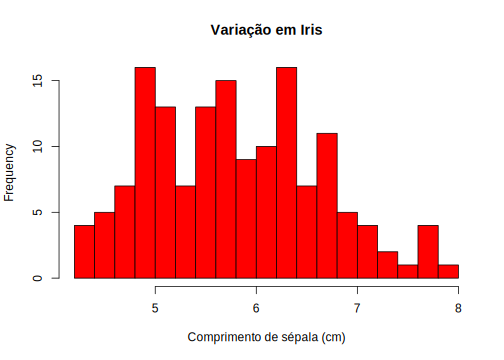
\includegraphics{bot89-introR_files/figure-latex/unnamed-chunk-262-1.pdf}

\begin{Shaded}
\begin{Highlighting}[]
\CommentTok{\# note que o eixo y é a frequencia que o valor ocorre, ou seja, corresponde ao número de linhas em iris que tem valor}
\end{Highlighting}
\end{Shaded}

\subsection{\texorpdfstring{\texttt{boxplot()}}{boxplot()}}\label{boxplot}

Esta função é importante por mostrar a variação em uma variável qualquer em relação às categorias de um fator.
É uma das melhores formas gráficas para mostrar a distribuição de valores de uma variável em relação às categorias.

\begin{Shaded}
\begin{Highlighting}[]
\NormalTok{?boxplot}
\end{Highlighting}
\end{Shaded}

\begin{Shaded}
\begin{Highlighting}[]
\CommentTok{\# vamos usar o objeto iris}
\FunctionTok{class}\NormalTok{(iris}\SpecialCharTok{$}\NormalTok{Sepal.Length) }\CommentTok{\# é um vetor}
\end{Highlighting}
\end{Shaded}

\begin{verbatim}
## [1] "numeric"
\end{verbatim}

\begin{Shaded}
\begin{Highlighting}[]
\FunctionTok{class}\NormalTok{(iris}\SpecialCharTok{$}\NormalTok{Species) }\CommentTok{\# é um fator}
\end{Highlighting}
\end{Shaded}

\begin{verbatim}
## [1] "factor"
\end{verbatim}

\begin{Shaded}
\begin{Highlighting}[]
\FunctionTok{boxplot}\NormalTok{(iris}\SpecialCharTok{$}\NormalTok{Sepal.Length }\SpecialCharTok{\textasciitilde{}}\NormalTok{ iris}\SpecialCharTok{$}\NormalTok{Species, }\AttributeTok{ylab =} \StringTok{"Comprimento da sépala"}\NormalTok{)}
\end{Highlighting}
\end{Shaded}

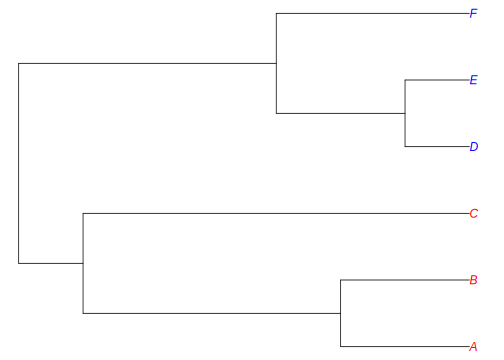
\includegraphics{bot89-introR_files/figure-latex/unnamed-chunk-264-1.pdf}

\begin{Shaded}
\begin{Highlighting}[]
\CommentTok{\# você pode fazer a mesma coisa com a função plot() porque ela é genérica que irá reconhecer que sua fórmula \textquotesingle{}valores\textasciitilde{}fator\textquotesingle{} pede por um boxplot}
\FunctionTok{plot}\NormalTok{(iris}\SpecialCharTok{$}\NormalTok{Sepal.Length }\SpecialCharTok{\textasciitilde{}}\NormalTok{ iris}\SpecialCharTok{$}\NormalTok{Species, }\AttributeTok{ylab =} \StringTok{"Comprimento da sépala"}\NormalTok{, }\AttributeTok{xlab =} \StringTok{""}\NormalTok{) }\CommentTok{\# note que especificamos aqui que o eixo x não tem título (lab)}
\end{Highlighting}
\end{Shaded}

\includegraphics{bot89-introR_files/figure-latex/unnamed-chunk-264-2.pdf}

\subsection{\texorpdfstring{\texttt{barplot()}}{barplot()}}\label{barplot}

Esta função gera um gráfico de barras simples.

\begin{Shaded}
\begin{Highlighting}[]
\NormalTok{?barplot }\CommentTok{\# veja o help dessa função}
\NormalTok{?VADeaths }\CommentTok{\# veja o help desse conjunto de dados}
\end{Highlighting}
\end{Shaded}

\begin{Shaded}
\begin{Highlighting}[]
\FunctionTok{class}\NormalTok{(VADeaths)}
\end{Highlighting}
\end{Shaded}

\begin{verbatim}
## [1] "matrix" "array"
\end{verbatim}

\begin{Shaded}
\begin{Highlighting}[]
\NormalTok{VADeaths }\CommentTok{\# taxas de mortalidade/1000 habitantes no estado da Virgínia em 1940}
\end{Highlighting}
\end{Shaded}

\begin{tabular}{l|r|r|r|r}
\hline
  & Rural Male & Rural Female & Urban Male & Urban Female\\
\hline
50-54 & 11.7 & 8.7 & 15.4 & 8.4\\
\hline
55-59 & 18.1 & 11.7 & 24.3 & 13.6\\
\hline
60-64 & 26.9 & 20.3 & 37.0 & 19.3\\
\hline
65-69 & 41.0 & 30.9 & 54.6 & 35.1\\
\hline
70-74 & 66.0 & 54.3 & 71.1 & 50.0\\
\hline
\end{tabular}

\begin{Shaded}
\begin{Highlighting}[]
\FunctionTok{rownames}\NormalTok{(VADeaths) }\CommentTok{\# cada linha é uma classe de idade}
\end{Highlighting}
\end{Shaded}

\begin{verbatim}
## [1] "50-54" "55-59" "60-64" "65-69" "70-74"
\end{verbatim}

\begin{Shaded}
\begin{Highlighting}[]
\FunctionTok{colnames}\NormalTok{(VADeaths) }\CommentTok{\# cada coluna é sexo e cidade ou rural}
\end{Highlighting}
\end{Shaded}

\begin{verbatim}
## [1] "Rural Male"   "Rural Female" "Urban Male"   "Urban Female"
\end{verbatim}

\begin{Shaded}
\begin{Highlighting}[]
\CommentTok{\# com as informações padrão}
\FunctionTok{barplot}\NormalTok{(VADeaths) }\CommentTok{\# cada cor é uma linha}
\end{Highlighting}
\end{Shaded}

\includegraphics{bot89-introR_files/figure-latex/unnamed-chunk-266-1.pdf}

\begin{Shaded}
\begin{Highlighting}[]
\FunctionTok{barplot}\NormalTok{(VADeaths, }\AttributeTok{beside =} \ConstantTok{TRUE}\NormalTok{) }\CommentTok{\# lado a lado (cada barra é uma linha)}
\end{Highlighting}
\end{Shaded}

\includegraphics{bot89-introR_files/figure-latex/unnamed-chunk-266-2.pdf}

\begin{Shaded}
\begin{Highlighting}[]
\CommentTok{\# vamos colorir diferente, uma para cada linha}
\FunctionTok{rownames}\NormalTok{(VADeaths)}
\end{Highlighting}
\end{Shaded}

\begin{verbatim}
## [1] "50-54" "55-59" "60-64" "65-69" "70-74"
\end{verbatim}

\begin{Shaded}
\begin{Highlighting}[]
\NormalTok{cores }\OtherTok{\textless{}{-}} \FunctionTok{rainbow}\NormalTok{(}\AttributeTok{n =} \FunctionTok{nrow}\NormalTok{(VADeaths))}
\NormalTok{cores }\CommentTok{\# uma cor por linha}
\end{Highlighting}
\end{Shaded}

\begin{verbatim}
## [1] "#FF0000" "#CCFF00" "#00FF66" "#0066FF" "#CC00FF"
\end{verbatim}

\begin{Shaded}
\begin{Highlighting}[]
\CommentTok{\# essa é a correspondencia:}
\FunctionTok{cbind}\NormalTok{(}\FunctionTok{rownames}\NormalTok{(VADeaths), cores)}
\end{Highlighting}
\end{Shaded}

\begin{tabular}{l|l}
\hline
 & cores\\
\hline
50-54 & \#FF0000\\
\hline
55-59 & \#CCFF00\\
\hline
60-64 & \#00FF66\\
\hline
65-69 & \#0066FF\\
\hline
70-74 & \#CC00FF\\
\hline
\end{tabular}

\begin{Shaded}
\begin{Highlighting}[]
\CommentTok{\# plota com essas cores}
\FunctionTok{barplot}\NormalTok{(VADeaths, }\AttributeTok{beside =} \ConstantTok{TRUE}\NormalTok{, }\AttributeTok{col =}\NormalTok{ cores)}
\end{Highlighting}
\end{Shaded}

\includegraphics{bot89-introR_files/figure-latex/unnamed-chunk-266-3.pdf}

\subsection{\texorpdfstring{\texttt{plot.phylo()}}{plot.phylo()}}\label{plot.phylo}

O pacote \href{https://cran.r-project.org/web/packages/ape/index.html}{Ape (Analyses of Phylogenetics and Evolution)} \citep{R-ape} possui uma função para desenhar uma filogenia.
Caso você não tenha instalado o pacote \texttt{ape} ainda, faça-o assim:

\begin{Shaded}
\begin{Highlighting}[]
\FunctionTok{install.packages}\NormalTok{(}\StringTok{"ape"}\NormalTok{)}
\end{Highlighting}
\end{Shaded}

Depois, siga o exemplo abaixo:

\begin{Shaded}
\begin{Highlighting}[]
\FunctionTok{library}\NormalTok{(ape) }\CommentTok{\# chama o pacote}

\CommentTok{\# uma filogenia hipotética para exemplo}
\NormalTok{arv }\OtherTok{\textless{}{-}} \StringTok{"(((A:1,B:1):2,C:3):0.5,((D:0.5,E:0.5):1,F:1.5):2);"}

\CommentTok{\# lê essa filogenia para um objeto de classe phylo, que é uma classe para dendrogramas.}
\NormalTok{phy }\OtherTok{\textless{}{-}} \FunctionTok{read.tree}\NormalTok{(}\AttributeTok{text =}\NormalTok{ arv)}
\FunctionTok{class}\NormalTok{(phy)}
\end{Highlighting}
\end{Shaded}

\begin{verbatim}
## [1] "phylo"
\end{verbatim}

\begin{Shaded}
\begin{Highlighting}[]
\CommentTok{\# podemos plotar essa filogenia com}
\FunctionTok{plot}\NormalTok{(phy)}
\end{Highlighting}
\end{Shaded}

\includegraphics{bot89-introR_files/figure-latex/unnamed-chunk-268-1.pdf}

\begin{Shaded}
\begin{Highlighting}[]
\CommentTok{\# porque a função plot reconhece}
\CommentTok{\# que objetos de classe "phylo" são árvores}
\CommentTok{\# de fato ela usa a função plot.phylo() para gerar essa figura, que contém argumentos específicos para objetos dessa classe}
\end{Highlighting}
\end{Shaded}

\begin{Shaded}
\begin{Highlighting}[]
\NormalTok{?plot.phylo }\CommentTok{\# veja o help e os argumentos}
\end{Highlighting}
\end{Shaded}

\begin{Shaded}
\begin{Highlighting}[]
\CommentTok{\# portanto posso incluir argumentos de plot.phylo() quando uso a função plot() para plotar um objeto de classe phylo}
\FunctionTok{plot}\NormalTok{(phy, }\AttributeTok{no.margin =} \ConstantTok{TRUE}\NormalTok{, }\AttributeTok{tip.color =} \FunctionTok{c}\NormalTok{(}\FunctionTok{rep}\NormalTok{(}\StringTok{"red"}\NormalTok{, }\DecValTok{3}\NormalTok{), }\FunctionTok{rep}\NormalTok{(}\StringTok{"blue"}\NormalTok{, }\DecValTok{3}\NormalTok{)))}
\end{Highlighting}
\end{Shaded}

\includegraphics{bot89-introR_files/figure-latex/unnamed-chunk-270-1.pdf}

\begin{Shaded}
\begin{Highlighting}[]
\CommentTok{\# seria o mesmo que dizer}
\FunctionTok{plot.phylo}\NormalTok{(phy, }\AttributeTok{no.margin =} \ConstantTok{TRUE}\NormalTok{, }\AttributeTok{tip.color =} \FunctionTok{c}\NormalTok{(}\FunctionTok{rep}\NormalTok{(}\StringTok{"red"}\NormalTok{, }\DecValTok{3}\NormalTok{), }\FunctionTok{rep}\NormalTok{(}\StringTok{"blue"}\NormalTok{, }\DecValTok{3}\NormalTok{)))}
\end{Highlighting}
\end{Shaded}

\subsection{\texorpdfstring{\texttt{image()} e \texttt{countour()}}{image() e countour()}}\label{image-e-countour}

\begin{Shaded}
\begin{Highlighting}[]
\CommentTok{\# existe um conjunto de dados topográficos na base do R que vamos usar como exemplo}
\FunctionTok{class}\NormalTok{(volcano) }\CommentTok{\# é uma matriz}
\FunctionTok{dim}\NormalTok{(volcano) }\CommentTok{\# com 87 linhas e 61 uma colnas}
\NormalTok{volcano[}\DecValTok{1}\SpecialCharTok{:}\DecValTok{5}\NormalTok{, }\DecValTok{1}\SpecialCharTok{:}\DecValTok{5}\NormalTok{] }\CommentTok{\# os valores são altitude}
\FunctionTok{hist}\NormalTok{(volcano, }\AttributeTok{breaks =} \DecValTok{20}\NormalTok{) }\CommentTok{\# essa é a distribuição de valores de elevacao}
\FunctionTok{range}\NormalTok{(volcano) }\CommentTok{\# amplitude de variação}
\end{Highlighting}
\end{Shaded}

\begin{Shaded}
\begin{Highlighting}[]
\CommentTok{\# podemos usar algumas funções para visualizar um conjunto de dados que tem essa estrutura (matrix)}
\NormalTok{?image }\CommentTok{\# veja o help}
\end{Highlighting}
\end{Shaded}

\begin{Shaded}
\begin{Highlighting}[]
\FunctionTok{image}\NormalTok{(volcano, }\AttributeTok{col =} \FunctionTok{heat.colors}\NormalTok{(}\DecValTok{12}\NormalTok{))}
\end{Highlighting}
\end{Shaded}

\includegraphics{bot89-introR_files/figure-latex/unnamed-chunk-273-1.pdf}

\begin{Shaded}
\begin{Highlighting}[]
\NormalTok{?heat.colors }\CommentTok{\# veja opções de gradientes continuos de cores}
\end{Highlighting}
\end{Shaded}

\begin{Shaded}
\begin{Highlighting}[]
\CommentTok{\# vamos mudar isso,}
\NormalTok{cores }\OtherTok{\textless{}{-}} \FunctionTok{terrain.colors}\NormalTok{(}\DecValTok{12}\NormalTok{) }\CommentTok{\# 12 categorias de cores}
\NormalTok{cores }\CommentTok{\# o código é uma cor em HTML}
\end{Highlighting}
\end{Shaded}

\begin{verbatim}
##  [1] "#00A600" "#24B300" "#4CBF00" "#7ACC00" "#ADD900" "#E6E600" "#E8C727"
##  [8] "#EAB64E" "#ECB176" "#EEB99F" "#F0CFC8" "#F2F2F2"
\end{verbatim}

\begin{Shaded}
\begin{Highlighting}[]
\FunctionTok{image}\NormalTok{(volcano, }\AttributeTok{col =}\NormalTok{ cores)}
\end{Highlighting}
\end{Shaded}

\includegraphics{bot89-introR_files/figure-latex/unnamed-chunk-275-1.pdf}

\begin{Shaded}
\begin{Highlighting}[]
\CommentTok{\# notem a cratera}
\end{Highlighting}
\end{Shaded}

\begin{Shaded}
\begin{Highlighting}[]
\NormalTok{?contour }\CommentTok{\# veja o help}
\end{Highlighting}
\end{Shaded}

\begin{Shaded}
\begin{Highlighting}[]
\CommentTok{\# outra opção é fazermos os contornos (ou curvas de nível neste caso do vulcão)}
\FunctionTok{contour}\NormalTok{(volcano)}
\end{Highlighting}
\end{Shaded}

\includegraphics{bot89-introR_files/figure-latex/unnamed-chunk-277-1.pdf}

\begin{Shaded}
\begin{Highlighting}[]
\CommentTok{\# vamos mudar o número de níveis para o mesmo usado para as cores}
\FunctionTok{contour}\NormalTok{(volcano, }\AttributeTok{nlevels =} \DecValTok{12}\NormalTok{)}

\CommentTok{\# vamos juntar essas figuras em uma só}
\FunctionTok{image}\NormalTok{(volcano, }\AttributeTok{col =}\NormalTok{ cores)}
\FunctionTok{contour}\NormalTok{(volcano, }\AttributeTok{nlevels =} \DecValTok{12}\NormalTok{, }\AttributeTok{add =} \ConstantTok{TRUE}\NormalTok{)}
\end{Highlighting}
\end{Shaded}

\includegraphics{bot89-introR_files/figure-latex/unnamed-chunk-277-2.pdf}

\begin{Shaded}
\begin{Highlighting}[]
\CommentTok{\# note o argumento add=TRUE que indica para a função de alto{-}nível}
\CommentTok{\# que ela não deve começar uma nova figura,}
\CommentTok{\# apenas adiciona à uma já criada por outra função de alto{-}nível}
\CommentTok{\# muitas funções de alto{-}nível tem esse argumento add, que, portanto, mimetiza o que função gráfica de baixo{-}nível faz}
\end{Highlighting}
\end{Shaded}

\subsection{\texorpdfstring{\texttt{map()}}{map()}}\label{map}

O pacote \href{https://cran.r-project.org/web/packages/maps/index.html}{maps} \citep{R-maps} fornece funções para desenhar mapas com divisões administrativas.
A função \texttt{map()} é uma de alto-nível.
Veremos depois como adicionar sobre esses mapas informação através de funções de baixo-nível.

\begin{Shaded}
\begin{Highlighting}[]
\NormalTok{?maps}\SpecialCharTok{::}\NormalTok{map }\CommentTok{\# veja o help}
\end{Highlighting}
\end{Shaded}

Caso você não tenha instalado o pacote \texttt{maps} ainda, faça-o assim:

\begin{Shaded}
\begin{Highlighting}[]
\FunctionTok{install.packages}\NormalTok{(}\StringTok{"maps"}\NormalTok{)}
\end{Highlighting}
\end{Shaded}

Agora, siga o exemplo abaixo:

\begin{Shaded}
\begin{Highlighting}[]
\FunctionTok{library}\NormalTok{(maps) }\CommentTok{\# instalar se não tiver instalado}
\FunctionTok{map}\NormalTok{() }\CommentTok{\# mapa do mundo}
\end{Highlighting}
\end{Shaded}

\includegraphics{bot89-introR_files/figure-latex/unnamed-chunk-280-1.pdf}

\begin{Shaded}
\begin{Highlighting}[]
\FunctionTok{map}\NormalTok{(}\AttributeTok{region =} \StringTok{"Brazil"}\NormalTok{) }\CommentTok{\# Brazil}
\end{Highlighting}
\end{Shaded}

\includegraphics{bot89-introR_files/figure-latex/unnamed-chunk-280-2.pdf}

\begin{Shaded}
\begin{Highlighting}[]
\CommentTok{\# dev.off() \#pode precisar fechar o dispositivo se estiver avisar que a figura é muito grande}

\FunctionTok{dev.off}\NormalTok{()}
\end{Highlighting}
\end{Shaded}

\begin{verbatim}
## null device 
##           1
\end{verbatim}

\begin{Shaded}
\begin{Highlighting}[]
\NormalTok{sa }\OtherTok{\textless{}{-}} \FunctionTok{c}\NormalTok{(}\StringTok{"Brazil"}\NormalTok{, }\StringTok{"Guyana"}\NormalTok{, }\StringTok{"French Guiana"}\NormalTok{, }\StringTok{"Suriname"}\NormalTok{, }\StringTok{"Venezuela"}\NormalTok{, }\StringTok{"Colombia"}\NormalTok{, }\StringTok{"Ecuador"}\NormalTok{, }\StringTok{"Trinidad{-}Tobago"}\NormalTok{, }\StringTok{"Peru"}\NormalTok{, }\StringTok{"Bolivia"}\NormalTok{, }\StringTok{"Paraguay"}\NormalTok{, }\StringTok{"Chile"}\NormalTok{, }\StringTok{"Argentina"}\NormalTok{, }\StringTok{"Uruguay"}\NormalTok{, }\StringTok{"Panama"}\NormalTok{)}
\FunctionTok{map}\NormalTok{(}\AttributeTok{region =}\NormalTok{ sa, }\AttributeTok{col =} \StringTok{"red"}\NormalTok{, }\AttributeTok{lty =} \StringTok{"dashed"}\NormalTok{)}
\end{Highlighting}
\end{Shaded}

\subsection{\texorpdfstring{\texttt{xlim} e \texttt{ylim}}{xlim e ylim}}\label{xlim-e-ylim}

Esses dois parâmetros gráficos permitem ajustar o tamanho dos eixos de um gráfico, impondo limites.

\begin{Shaded}
\begin{Highlighting}[]
\CommentTok{\# CONTROLANDO UM XLIM}
\FunctionTok{plot}\NormalTok{(iris}\SpecialCharTok{$}\NormalTok{Sepal.Length, iris}\SpecialCharTok{$}\NormalTok{Sepal.Width, }\AttributeTok{pch =} \DecValTok{21}\NormalTok{, }\AttributeTok{col =} \StringTok{"red"}\NormalTok{)}
\CommentTok{\# vamos aumentar um pouco o eixo X}
\NormalTok{rg }\OtherTok{\textless{}{-}} \FunctionTok{range}\NormalTok{(iris}\SpecialCharTok{$}\NormalTok{Sepal.Length) }\CommentTok{\# variacao atual}
\NormalTok{rg}
\CommentTok{\# aumentar}
\NormalTok{rg2 }\OtherTok{\textless{}{-}}\NormalTok{ rg }\SpecialCharTok{+} \FunctionTok{c}\NormalTok{(}\SpecialCharTok{{-}}\DecValTok{1}\NormalTok{, }\SpecialCharTok{+}\DecValTok{1}\NormalTok{) }\CommentTok{\# adicionamos 1 unidade de cada lado}
\NormalTok{rg2}
\FunctionTok{plot}\NormalTok{(iris}\SpecialCharTok{$}\NormalTok{Sepal.Length, iris}\SpecialCharTok{$}\NormalTok{Sepal.Width, }\AttributeTok{pch =} \DecValTok{21}\NormalTok{, }\AttributeTok{col =} \StringTok{"red"}\NormalTok{, }\AttributeTok{xlim =}\NormalTok{ rg2)}


\CommentTok{\# LIMITANDO UM MAPA POR SUAS COORDENADAS}
\FunctionTok{dev.off}\NormalTok{()}
\FunctionTok{library}\NormalTok{(maps) }\CommentTok{\# instalar se não tiver instalado}
\FunctionTok{map}\NormalTok{() }\CommentTok{\# mapa do mundo}
\CommentTok{\# alguns limites em latitude e longitude}
\NormalTok{lat0 }\OtherTok{\textless{}{-}} \SpecialCharTok{{-}}\DecValTok{22}
\NormalTok{lat1 }\OtherTok{\textless{}{-}} \DecValTok{5}
\NormalTok{long0 }\OtherTok{\textless{}{-}} \SpecialCharTok{{-}}\DecValTok{80}
\NormalTok{long1 }\OtherTok{\textless{}{-}} \SpecialCharTok{{-}}\DecValTok{30}
\FunctionTok{dev.off}\NormalTok{()}
\FunctionTok{map}\NormalTok{(}\AttributeTok{xlim =} \FunctionTok{c}\NormalTok{(long0, long1), }\AttributeTok{ylim =} \FunctionTok{c}\NormalTok{(lat0, lat1))}
\end{Highlighting}
\end{Shaded}

\section{Funções gráficas de baixo nível}\label{graf-baixo-nivel}

Funções de baixo nível são funções que permitem \textbf{ADICIONAR} elementos em um gráfico já aberto com as funções \texttt{plot()} ou \texttt{plot.new()}.
Muitas vezes você pode usar uma função de alto nível para fazer a mesma coisa com o argumento \texttt{add\ =\ TRUE}.
Vamos ver alguns exemplos mais comumente utilizados de funções de baixo-nível.

\subsection{\texorpdfstring{\texttt{legend()}}{legend()}}\label{legend}

A função \texttt{legend()} permite colocar uma legenda sobre um gráfico aberto por uma função de alto nível.

\begin{Shaded}
\begin{Highlighting}[]
\NormalTok{?legend }\CommentTok{\# veja o help dessa funcao}
\CommentTok{\# vamos usar iris novamente}
\end{Highlighting}
\end{Shaded}

\begin{Shaded}
\begin{Highlighting}[]
\NormalTok{Sepalas }\OtherTok{\textless{}{-}}\NormalTok{ iris}\SpecialCharTok{$}\NormalTok{Sepal.Length}
\NormalTok{Petalas }\OtherTok{\textless{}{-}}\NormalTok{ iris}\SpecialCharTok{$}\NormalTok{Petal.Length}
\FunctionTok{nlevels}\NormalTok{(iris}\SpecialCharTok{$}\NormalTok{Species) }\CommentTok{\# contém três espécies}
\end{Highlighting}
\end{Shaded}

\begin{verbatim}
## [1] 3
\end{verbatim}

\begin{Shaded}
\begin{Highlighting}[]
\FunctionTok{levels}\NormalTok{(iris}\SpecialCharTok{$}\NormalTok{Species)}
\end{Highlighting}
\end{Shaded}

\begin{verbatim}
## [1] "setosa"     "versicolor" "virginica"
\end{verbatim}

\begin{Shaded}
\begin{Highlighting}[]
\NormalTok{ascores }\OtherTok{\textless{}{-}} \FunctionTok{c}\NormalTok{(}\StringTok{"red"}\NormalTok{, }\StringTok{"blue"}\NormalTok{, }\StringTok{"green"}\NormalTok{)[}\FunctionTok{as.numeric}\NormalTok{(iris}\SpecialCharTok{$}\NormalTok{Species)]}
\CommentTok{\# plota a figura}
\FunctionTok{plot}\NormalTok{(Sepalas, Petalas, }\AttributeTok{pch =} \DecValTok{21}\NormalTok{, }\AttributeTok{bg =}\NormalTok{ ascores, }\AttributeTok{cex =} \FloatTok{0.8}\NormalTok{)}

\CommentTok{\# vamos colocar uma legenda no canto direito inferior}
\CommentTok{\# definimos o que vai na legenda}
\NormalTok{cores }\OtherTok{\textless{}{-}} \FunctionTok{c}\NormalTok{(}\StringTok{"red"}\NormalTok{, }\StringTok{"blue"}\NormalTok{, }\StringTok{"green"}\NormalTok{)}
\NormalTok{texto }\OtherTok{\textless{}{-}} \FunctionTok{levels}\NormalTok{(iris}\SpecialCharTok{$}\NormalTok{Species)}
\FunctionTok{legend}\NormalTok{(}\StringTok{"bottomright"}\NormalTok{, }\AttributeTok{legend =}\NormalTok{ texto, }\AttributeTok{pt.bg =}\NormalTok{ cores, }\AttributeTok{pch =} \DecValTok{21}\NormalTok{)}
\end{Highlighting}
\end{Shaded}

\includegraphics{bot89-introR_files/figure-latex/unnamed-chunk-283-1.pdf}

\begin{Shaded}
\begin{Highlighting}[]
\CommentTok{\# ficou apertado né...}
\CommentTok{\# aumentar o espacamento, colocar mais para dentro e tirar o box, diminuir o texto, aumentar o tamanho do ponto}
\CommentTok{\# plota a figura}
\FunctionTok{plot}\NormalTok{(Sepalas, Petalas, }\AttributeTok{pch =} \DecValTok{21}\NormalTok{, }\AttributeTok{bg =}\NormalTok{ ascores, }\AttributeTok{cex =} \FloatTok{0.8}\NormalTok{)}
\FunctionTok{legend}\NormalTok{(}\StringTok{"bottomright"}\NormalTok{, }\AttributeTok{legend =}\NormalTok{ texto, }\AttributeTok{pt.bg =}\NormalTok{ cores, }\AttributeTok{pch =} \DecValTok{21}\NormalTok{, }\AttributeTok{y.intersp =} \FloatTok{1.7}\NormalTok{, }\AttributeTok{inset =} \FloatTok{0.1}\NormalTok{, }\AttributeTok{box.lwd =} \DecValTok{0}\NormalTok{, }\AttributeTok{cex =} \FloatTok{0.8}\NormalTok{, }\AttributeTok{pt.cex =} \FloatTok{1.5}\NormalTok{)}
\end{Highlighting}
\end{Shaded}

\includegraphics{bot89-introR_files/figure-latex/unnamed-chunk-283-2.pdf}

\begin{Shaded}
\begin{Highlighting}[]
\CommentTok{\# podemos colocar legendas também pela coordenada}
\FunctionTok{plot}\NormalTok{(Sepalas, Petalas, }\AttributeTok{pch =} \DecValTok{21}\NormalTok{, }\AttributeTok{bg =}\NormalTok{ ascores, }\AttributeTok{cex =} \FloatTok{0.8}\NormalTok{)}
\FunctionTok{legend}\NormalTok{(}\AttributeTok{x =} \DecValTok{7}\NormalTok{, }\AttributeTok{y =} \DecValTok{3}\NormalTok{, }\AttributeTok{legend =}\NormalTok{ texto, }\AttributeTok{pt.bg =}\NormalTok{ cores, }\AttributeTok{pch =} \DecValTok{21}\NormalTok{, }\AttributeTok{y.intersp =} \FloatTok{1.7}\NormalTok{, }\AttributeTok{inset =} \FloatTok{0.1}\NormalTok{, }\AttributeTok{box.lwd =} \DecValTok{0}\NormalTok{, }\AttributeTok{cex =} \FloatTok{0.8}\NormalTok{, }\AttributeTok{pt.cex =} \FloatTok{1.5}\NormalTok{)}
\end{Highlighting}
\end{Shaded}

\includegraphics{bot89-introR_files/figure-latex/unnamed-chunk-283-3.pdf}

\begin{Shaded}
\begin{Highlighting}[]
\CommentTok{\# ou colocar fora da figura}
\CommentTok{\# neste caso, primeiro dividimos o dispositivo em tres partes e plotamos a figura em 2 partes e a legenda em 1 parte}
\FunctionTok{layout}\NormalTok{(}\FunctionTok{matrix}\NormalTok{(}\FunctionTok{c}\NormalTok{(}\DecValTok{1}\NormalTok{, }\DecValTok{1}\NormalTok{, }\DecValTok{2}\NormalTok{), }\AttributeTok{nrow =} \DecValTok{1}\NormalTok{, }\AttributeTok{ncol =} \DecValTok{3}\NormalTok{))}
\FunctionTok{plot}\NormalTok{(Sepalas, Petalas, }\AttributeTok{pch =} \DecValTok{21}\NormalTok{, }\AttributeTok{bg =}\NormalTok{ ascores, }\AttributeTok{cex =} \FloatTok{0.8}\NormalTok{)}
\CommentTok{\# usamos a função plot.new() para mudar de parte no dispositivo cirando um plot vazio}
\FunctionTok{plot.new}\NormalTok{() }\CommentTok{\# nao vai ver nada acontecendo}
\CommentTok{\# agora plotamos a legenda nesse espaço}
\FunctionTok{legend}\NormalTok{(}\StringTok{"left"}\NormalTok{, }\AttributeTok{legend =}\NormalTok{ texto, }\AttributeTok{pt.bg =}\NormalTok{ cores, }\AttributeTok{pch =} \DecValTok{21}\NormalTok{, }\AttributeTok{y.intersp =} \FloatTok{1.7}\NormalTok{, }\AttributeTok{inset =} \FloatTok{0.1}\NormalTok{, }\AttributeTok{box.lwd =} \DecValTok{0}\NormalTok{, }\AttributeTok{cex =} \FloatTok{0.8}\NormalTok{, }\AttributeTok{pt.cex =} \FloatTok{1.5}\NormalTok{)}
\end{Highlighting}
\end{Shaded}

\includegraphics{bot89-introR_files/figure-latex/unnamed-chunk-283-4.pdf}

\subsection{\texorpdfstring{\texttt{points()}}{points()}}\label{points}

Esta função genérica serve para adicionar pontos, linhas, simbolos etc, segundo coordenadas \texttt{x} ou \texttt{x+y} em um gráfico aberto por uma função de alto nível.

\begin{Shaded}
\begin{Highlighting}[]
\FunctionTok{layout}\NormalTok{(}\DecValTok{1}\NormalTok{) }\CommentTok{\# restaurando para 1 se fez o script acima}
\CommentTok{\# vamos usar um conjunto de dados de crescimento de laranja}
\FunctionTok{data}\NormalTok{(}\StringTok{"Orange"}\NormalTok{)}
\FunctionTok{colnames}\NormalTok{(Orange) }\CommentTok{\# número da árvore, idade, circunferencia nessa idade}
\end{Highlighting}
\end{Shaded}

\begin{verbatim}
## [1] "Tree"          "age"           "circumference"
\end{verbatim}

\begin{Shaded}
\begin{Highlighting}[]
\FunctionTok{head}\NormalTok{(Orange)}
\end{Highlighting}
\end{Shaded}

\begin{tabular}{l|r|r}
\hline
Tree & age & circumference\\
\hline
1 & 118 & 30\\
\hline
1 & 484 & 58\\
\hline
1 & 664 & 87\\
\hline
1 & 1004 & 115\\
\hline
1 & 1231 & 120\\
\hline
1 & 1372 & 142\\
\hline
\end{tabular}

\begin{Shaded}
\begin{Highlighting}[]
\FunctionTok{unique}\NormalTok{(Orange}\SpecialCharTok{$}\NormalTok{Tree) }\CommentTok{\# tem cinco árvores}
\end{Highlighting}
\end{Shaded}

\begin{verbatim}
## [1] 1 2 3 4 5
## Levels: 3 < 1 < 5 < 2 < 4
\end{verbatim}

\begin{Shaded}
\begin{Highlighting}[]
\CommentTok{\# vamos plotar idade por circunferencia}
\CommentTok{\# uma linha por árvore}
\CommentTok{\# cada linha de um tipo e cor diferente}

\CommentTok{\# definir tipos de linhas e cores}
\NormalTok{ascores }\OtherTok{\textless{}{-}} \FunctionTok{c}\NormalTok{(}\StringTok{"red"}\NormalTok{, }\StringTok{"blue"}\NormalTok{, }\StringTok{"green"}\NormalTok{, }\StringTok{"yellow"}\NormalTok{, }\StringTok{"purple"}\NormalTok{)}
\NormalTok{linhatipos }\OtherTok{\textless{}{-}} \FunctionTok{c}\NormalTok{(}\StringTok{"solid"}\NormalTok{, }\StringTok{"dashed"}\NormalTok{, }\StringTok{"dotted"}\NormalTok{, }\StringTok{"dotdash"}\NormalTok{, }\StringTok{"longdash"}\NormalTok{)}

\CommentTok{\# uma cor por árvore}
\NormalTok{treeidx }\OtherTok{\textless{}{-}} \FunctionTok{as.numeric}\NormalTok{(Orange}\SpecialCharTok{$}\NormalTok{Tree)}
\NormalTok{cls }\OtherTok{\textless{}{-}}\NormalTok{ ascores[treeidx]}
\NormalTok{cls}
\end{Highlighting}
\end{Shaded}

\begin{verbatim}
##  [1] "blue"   "blue"   "blue"   "blue"   "blue"   "blue"   "blue"   "yellow"
##  [9] "yellow" "yellow" "yellow" "yellow" "yellow" "yellow" "red"    "red"   
## [17] "red"    "red"    "red"    "red"    "red"    "purple" "purple" "purple"
## [25] "purple" "purple" "purple" "purple" "green"  "green"  "green"  "green" 
## [33] "green"  "green"  "green"
\end{verbatim}

\begin{Shaded}
\begin{Highlighting}[]
\CommentTok{\# um tipo de linha por arvore}
\NormalTok{tps }\OtherTok{\textless{}{-}}\NormalTok{ linhatipos[treeidx]}
\NormalTok{tps}
\end{Highlighting}
\end{Shaded}

\begin{verbatim}
##  [1] "dashed"   "dashed"   "dashed"   "dashed"   "dashed"   "dashed"  
##  [7] "dashed"   "dotdash"  "dotdash"  "dotdash"  "dotdash"  "dotdash" 
## [13] "dotdash"  "dotdash"  "solid"    "solid"    "solid"    "solid"   
## [19] "solid"    "solid"    "solid"    "longdash" "longdash" "longdash"
## [25] "longdash" "longdash" "longdash" "longdash" "dotted"   "dotted"  
## [31] "dotted"   "dotted"   "dotted"   "dotted"   "dotted"
\end{verbatim}

\begin{Shaded}
\begin{Highlighting}[]
\CommentTok{\# fazemos uma figura}
\FunctionTok{plot}\NormalTok{(Orange}\SpecialCharTok{$}\NormalTok{age, Orange}\SpecialCharTok{$}\NormalTok{circumference, }\AttributeTok{lwd =} \DecValTok{1}\NormalTok{, }\AttributeTok{type =} \StringTok{"b"}\NormalTok{, }\AttributeTok{col =}\NormalTok{ cls, }\AttributeTok{lty =}\NormalTok{ tps)}
\end{Highlighting}
\end{Shaded}

\includegraphics{bot89-introR_files/figure-latex/unnamed-chunk-284-1.pdf}

\begin{Shaded}
\begin{Highlighting}[]
\CommentTok{\# note que todas as linhas sairam com primeira cor e com o primeiro tipo}
\NormalTok{cls[}\DecValTok{1}\NormalTok{]}
\end{Highlighting}
\end{Shaded}

\begin{verbatim}
## [1] "blue"
\end{verbatim}

\begin{Shaded}
\begin{Highlighting}[]
\NormalTok{tps[}\DecValTok{1}\NormalTok{]}
\end{Highlighting}
\end{Shaded}

\begin{verbatim}
## [1] "dashed"
\end{verbatim}

\begin{Shaded}
\begin{Highlighting}[]
\CommentTok{\# nao dá para fazer assim, porque não especificamos como os pontos se ligam}

\CommentTok{\# podemos no entanto colocar linha por linha}
\CommentTok{\# desenhamos o gráfico com uma função de alto nível com os dados, mas vazia}
\FunctionTok{plot}\NormalTok{(Orange}\SpecialCharTok{$}\NormalTok{age, Orange}\SpecialCharTok{$}\NormalTok{circumference, }\AttributeTok{type =} \StringTok{"n"}\NormalTok{, }\AttributeTok{xlab =} \StringTok{"Idade"}\NormalTok{, }\AttributeTok{ylab =} \StringTok{"Circunferência"}\NormalTok{)}
\CommentTok{\# adicionamo para cada árvore os pontos e as linhas}
\NormalTok{arvs }\OtherTok{\textless{}{-}} \FunctionTok{as.numeric}\NormalTok{(}\FunctionTok{levels}\NormalTok{(Orange}\SpecialCharTok{$}\NormalTok{Tree))}
\NormalTok{pts }\OtherTok{\textless{}{-}}\NormalTok{ arvs }\SpecialCharTok{+} \DecValTok{20} \CommentTok{\# simbolos para pontos}
\NormalTok{i }\OtherTok{\textless{}{-}} \DecValTok{1}
\ControlFlowTok{for}\NormalTok{ (i }\ControlFlowTok{in} \DecValTok{1}\SpecialCharTok{:}\FunctionTok{length}\NormalTok{(arvs)) \{ }\CommentTok{\# para cada arvore}
  \CommentTok{\# filtra os dados}
\NormalTok{  dd }\OtherTok{\textless{}{-}}\NormalTok{ Orange[Orange}\SpecialCharTok{$}\NormalTok{Tree }\SpecialCharTok{==}\NormalTok{ arvs[i], ]}
  \CommentTok{\# adiciona no gráfico aberto a linha e os pontos e uma vez (type=\textquotesingle{}b\textquotesingle{}, veja o argumento type)}
  \FunctionTok{points}\NormalTok{(dd}\SpecialCharTok{$}\NormalTok{age, dd}\SpecialCharTok{$}\NormalTok{circumference, }\AttributeTok{type =} \StringTok{"b"}\NormalTok{, }\AttributeTok{pch =}\NormalTok{ pts[arvs[i]], }\AttributeTok{lty =}\NormalTok{ linhatipos[arvs[i]], }\AttributeTok{lwd =} \DecValTok{1}\NormalTok{, }\AttributeTok{col =}\NormalTok{ ascores[arvs[i]], }\AttributeTok{bg =}\NormalTok{ ascores[arvs[i]])}
\NormalTok{\}}

\CommentTok{\# vamos adicionar uma legenda}
\NormalTok{txt }\OtherTok{\textless{}{-}} \FunctionTok{paste}\NormalTok{(}\StringTok{"tree"}\NormalTok{, arvs)}
\FunctionTok{legend}\NormalTok{(}\StringTok{"bottomright"}\NormalTok{, }\AttributeTok{inset =} \FloatTok{0.1}\NormalTok{, }\AttributeTok{box.lwd =} \DecValTok{0}\NormalTok{, }\AttributeTok{legend =}\NormalTok{ txt, }\AttributeTok{pch =}\NormalTok{ pts[arvs], }\AttributeTok{pt.bg =}\NormalTok{ ascores[arvs], }\AttributeTok{lty =}\NormalTok{ linhatipos[arvs], }\AttributeTok{col =}\NormalTok{ ascores[arvs], }\AttributeTok{y.intersp =} \FloatTok{1.5}\NormalTok{)}
\end{Highlighting}
\end{Shaded}

\includegraphics{bot89-introR_files/figure-latex/unnamed-chunk-284-2.pdf}

\subsection{\texorpdfstring{\texttt{text()} e \texttt{mtext()}}{text() e mtext()}}\label{text-e-mtext}

\texttt{text()} e \texttt{mtext()}- funções para plotar textos (\textgreater= 1 caracter de comprimento) sobre uma figura de alto nível. text() plota dentro da área da figura através de coordendas, mtext() plota fora da área da figura com indicação do lado (side) e da distância da linha dos eixos (line).

\begin{Shaded}
\begin{Highlighting}[]
\NormalTok{?text }\CommentTok{\# veja o help dessa função}
\CommentTok{\# vamos usar iris novamente}
\end{Highlighting}
\end{Shaded}

\begin{Shaded}
\begin{Highlighting}[]
\NormalTok{Sepalas }\OtherTok{\textless{}{-}}\NormalTok{ iris}\SpecialCharTok{$}\NormalTok{Sepal.Length}
\NormalTok{Petalas }\OtherTok{\textless{}{-}}\NormalTok{ iris}\SpecialCharTok{$}\NormalTok{Petal.Length}
\FunctionTok{nlevels}\NormalTok{(iris}\SpecialCharTok{$}\NormalTok{Species) }\CommentTok{\# contém três espécies}
\end{Highlighting}
\end{Shaded}

\begin{verbatim}
## [1] 3
\end{verbatim}

\begin{Shaded}
\begin{Highlighting}[]
\FunctionTok{levels}\NormalTok{(iris}\SpecialCharTok{$}\NormalTok{Species)}
\end{Highlighting}
\end{Shaded}

\begin{verbatim}
## [1] "setosa"     "versicolor" "virginica"
\end{verbatim}

\begin{Shaded}
\begin{Highlighting}[]
\NormalTok{ascores }\OtherTok{\textless{}{-}} \FunctionTok{c}\NormalTok{(}\StringTok{"red"}\NormalTok{, }\StringTok{"blue"}\NormalTok{, }\StringTok{"green"}\NormalTok{)[}\FunctionTok{as.numeric}\NormalTok{(iris}\SpecialCharTok{$}\NormalTok{Species)]}

\CommentTok{\# vamos dar um código de texto para cada especie (suas primeiras letras maiusculo)}
\FunctionTok{levels}\NormalTok{(iris}\SpecialCharTok{$}\NormalTok{Species)}
\end{Highlighting}
\end{Shaded}

\begin{verbatim}
## [1] "setosa"     "versicolor" "virginica"
\end{verbatim}

\begin{Shaded}
\begin{Highlighting}[]
\NormalTok{spp }\OtherTok{\textless{}{-}} \FunctionTok{toupper}\NormalTok{(}\FunctionTok{substr}\NormalTok{(iris}\SpecialCharTok{$}\NormalTok{Species, }\DecValTok{1}\NormalTok{, }\DecValTok{2}\NormalTok{))}
\NormalTok{spp}
\end{Highlighting}
\end{Shaded}

\begin{verbatim}
##   [1] "SE" "SE" "SE" "SE" "SE" "SE" "SE" "SE" "SE" "SE" "SE" "SE" "SE" "SE" "SE"
##  [16] "SE" "SE" "SE" "SE" "SE" "SE" "SE" "SE" "SE" "SE" "SE" "SE" "SE" "SE" "SE"
##  [31] "SE" "SE" "SE" "SE" "SE" "SE" "SE" "SE" "SE" "SE" "SE" "SE" "SE" "SE" "SE"
##  [46] "SE" "SE" "SE" "SE" "SE" "VE" "VE" "VE" "VE" "VE" "VE" "VE" "VE" "VE" "VE"
##  [61] "VE" "VE" "VE" "VE" "VE" "VE" "VE" "VE" "VE" "VE" "VE" "VE" "VE" "VE" "VE"
##  [76] "VE" "VE" "VE" "VE" "VE" "VE" "VE" "VE" "VE" "VE" "VE" "VE" "VE" "VE" "VE"
##  [91] "VE" "VE" "VE" "VE" "VE" "VE" "VE" "VE" "VE" "VE" "VI" "VI" "VI" "VI" "VI"
## [106] "VI" "VI" "VI" "VI" "VI" "VI" "VI" "VI" "VI" "VI" "VI" "VI" "VI" "VI" "VI"
## [121] "VI" "VI" "VI" "VI" "VI" "VI" "VI" "VI" "VI" "VI" "VI" "VI" "VI" "VI" "VI"
## [136] "VI" "VI" "VI" "VI" "VI" "VI" "VI" "VI" "VI" "VI" "VI" "VI" "VI" "VI" "VI"
\end{verbatim}

\begin{Shaded}
\begin{Highlighting}[]
\CommentTok{\# plota a figura, mas ao inves de simbolos adicionamos text}
\CommentTok{\# poderiamos fazer isso se spp fosse apenas 1 caractere}
\FunctionTok{plot}\NormalTok{(Sepalas, Petalas, }\AttributeTok{pch =}\NormalTok{ spp, }\AttributeTok{col =}\NormalTok{ ascores, }\AttributeTok{cex =} \FloatTok{0.8}\NormalTok{)}
\FunctionTok{legend}\NormalTok{(}\StringTok{"bottomright"}\NormalTok{, }\AttributeTok{legend =} \FunctionTok{levels}\NormalTok{(iris}\SpecialCharTok{$}\NormalTok{Species), }\AttributeTok{text.col =} \FunctionTok{c}\NormalTok{(}\StringTok{"red"}\NormalTok{, }\StringTok{"blue"}\NormalTok{, }\StringTok{"green"}\NormalTok{), }\AttributeTok{inset =} \FloatTok{0.1}\NormalTok{, }\AttributeTok{box.lwd =} \DecValTok{0}\NormalTok{, }\AttributeTok{y.intersp =} \FloatTok{1.5}\NormalTok{)}
\end{Highlighting}
\end{Shaded}

\includegraphics{bot89-introR_files/figure-latex/unnamed-chunk-286-1.pdf}

\begin{Shaded}
\begin{Highlighting}[]
\CommentTok{\# mas note que versicolor e virginica não se diferenciam, pois pch plota apenas 1 caractere quando o simbolo for texto}

\CommentTok{\# podemos, no entanto, usar a funcao text para isso}
\FunctionTok{plot}\NormalTok{(Sepalas, Petalas, }\AttributeTok{type =} \StringTok{"n"}\NormalTok{)}
\FunctionTok{text}\NormalTok{(Sepalas, Petalas, }\AttributeTok{labels =}\NormalTok{ spp, }\AttributeTok{col =}\NormalTok{ ascores, }\AttributeTok{cex =} \FloatTok{0.8}\NormalTok{)}
\NormalTok{txt }\OtherTok{\textless{}{-}} \FunctionTok{paste}\NormalTok{(}\StringTok{"Iris"}\NormalTok{, }\FunctionTok{levels}\NormalTok{(iris}\SpecialCharTok{$}\NormalTok{Species))}
\FunctionTok{legend}\NormalTok{(}\StringTok{"bottomright"}\NormalTok{, }\AttributeTok{legend =}\NormalTok{ txt, }\AttributeTok{text.col =} \FunctionTok{c}\NormalTok{(}\StringTok{"red"}\NormalTok{, }\StringTok{"blue"}\NormalTok{, }\StringTok{"green"}\NormalTok{), }\AttributeTok{inset =} \FloatTok{0.1}\NormalTok{, }\AttributeTok{box.lwd =} \DecValTok{0}\NormalTok{, }\AttributeTok{y.intersp =} \FloatTok{1.5}\NormalTok{)}

\CommentTok{\# posso usar essa função para adicionar qualquer texto, em qualquer coordenada}
\FunctionTok{text}\NormalTok{(}\FloatTok{4.5}\NormalTok{, }\DecValTok{6}\NormalTok{, }\AttributeTok{labels =} \StringTok{"Exemplo Iris"}\NormalTok{, }\AttributeTok{adj =} \DecValTok{0}\NormalTok{, }\AttributeTok{col =} \StringTok{"yellow"}\NormalTok{)}
\CommentTok{\# note o argumento adj que define o ajuste do texto em relacao à coordenada x y especificada (ajuste: 0 esquerda, 1 direita)}
\CommentTok{\# apenas o x}
\FunctionTok{text}\NormalTok{(}\AttributeTok{x =} \FloatTok{4.5}\NormalTok{, }\AttributeTok{y =} \DecValTok{6}\NormalTok{, }\AttributeTok{labels =} \StringTok{"Exemplo Iris"}\NormalTok{, }\AttributeTok{adj =} \DecValTok{1}\NormalTok{, }\AttributeTok{col =} \StringTok{"black"}\NormalTok{)}

\CommentTok{\# o x e o y do ajuste (dois valores em adj)}
\FunctionTok{text}\NormalTok{(}\AttributeTok{x =} \FloatTok{4.5}\NormalTok{, }\AttributeTok{y =} \DecValTok{6}\NormalTok{, }\AttributeTok{labels =} \StringTok{"Exemplo Iris"}\NormalTok{, }\AttributeTok{adj =} \FunctionTok{c}\NormalTok{(}\FloatTok{0.3}\NormalTok{, }\DecValTok{1}\NormalTok{), }\AttributeTok{col =} \StringTok{"purple"}\NormalTok{)}

\CommentTok{\# a funcao mtext plot for da área das coordenas da figura}
\CommentTok{\# lado superior}
\FunctionTok{mtext}\NormalTok{(}\AttributeTok{side =} \DecValTok{3}\NormalTok{, }\AttributeTok{text =} \StringTok{"A."}\NormalTok{, }\AttributeTok{line =} \DecValTok{1}\NormalTok{, }\AttributeTok{col =} \StringTok{"red"}\NormalTok{, }\AttributeTok{font =} \DecValTok{2}\NormalTok{, }\AttributeTok{cex =} \DecValTok{2}\NormalTok{)}
\CommentTok{\# lado superior esquerdo}
\FunctionTok{mtext}\NormalTok{(}\AttributeTok{side =} \DecValTok{3}\NormalTok{, }\AttributeTok{text =} \StringTok{"A."}\NormalTok{, }\AttributeTok{line =} \DecValTok{1}\NormalTok{, }\AttributeTok{col =} \StringTok{"red"}\NormalTok{, }\AttributeTok{font =} \DecValTok{2}\NormalTok{, }\AttributeTok{cex =} \DecValTok{2}\NormalTok{, }\AttributeTok{adj =} \DecValTok{0}\NormalTok{)}

\CommentTok{\# lado inferior direito}
\FunctionTok{mtext}\NormalTok{(}\AttributeTok{side =} \DecValTok{1}\NormalTok{, }\AttributeTok{text =} \StringTok{"B."}\NormalTok{, }\AttributeTok{line =} \DecValTok{1}\NormalTok{, }\AttributeTok{col =} \StringTok{"red"}\NormalTok{, }\AttributeTok{font =} \DecValTok{2}\NormalTok{, }\AttributeTok{cex =} \DecValTok{2}\NormalTok{, }\AttributeTok{adj =} \DecValTok{1}\NormalTok{)}
\CommentTok{\# mais para baixo}
\FunctionTok{mtext}\NormalTok{(}\AttributeTok{side =} \DecValTok{1}\NormalTok{, }\AttributeTok{text =} \StringTok{"B."}\NormalTok{, }\AttributeTok{line =} \FloatTok{2.5}\NormalTok{, }\AttributeTok{col =} \StringTok{"red"}\NormalTok{, }\AttributeTok{font =} \DecValTok{2}\NormalTok{, }\AttributeTok{cex =} \DecValTok{2}\NormalTok{, }\AttributeTok{adj =} \DecValTok{1}\NormalTok{)}

\CommentTok{\# lado direito superior}
\FunctionTok{mtext}\NormalTok{(}\AttributeTok{side =} \DecValTok{4}\NormalTok{, }\AttributeTok{text =} \StringTok{"C."}\NormalTok{, }\AttributeTok{line =} \DecValTok{1}\NormalTok{, }\AttributeTok{col =} \StringTok{"red"}\NormalTok{, }\AttributeTok{font =} \DecValTok{2}\NormalTok{, }\AttributeTok{cex =} \DecValTok{2}\NormalTok{, }\AttributeTok{adj =} \DecValTok{1}\NormalTok{)}

\CommentTok{\# lado direito no meio}
\FunctionTok{mtext}\NormalTok{(}\AttributeTok{side =} \DecValTok{4}\NormalTok{, }\AttributeTok{text =} \StringTok{"C."}\NormalTok{, }\AttributeTok{line =} \DecValTok{1}\NormalTok{, }\AttributeTok{col =} \StringTok{"red"}\NormalTok{, }\AttributeTok{font =} \DecValTok{2}\NormalTok{, }\AttributeTok{cex =} \DecValTok{2}\NormalTok{, }\AttributeTok{adj =} \FloatTok{0.5}\NormalTok{)}
\end{Highlighting}
\end{Shaded}

\includegraphics{bot89-introR_files/figure-latex/unnamed-chunk-286-2.pdf}

\subsection{\texorpdfstring{\texttt{axis()}}{axis()}}\label{axis}

A função \texttt{axis()} adiciona eixos individualmente.
É importante quando desejamos combinar dois gráficos em um só.

\begin{Shaded}
\begin{Highlighting}[]
\NormalTok{?axis}
\end{Highlighting}
\end{Shaded}

\begin{Shaded}
\begin{Highlighting}[]
\CommentTok{\# algumas vezes queremos adicionar eixos, ou formatar o eixo de uma forma individualizada}
\CommentTok{\# por exemplo, na seguinte figura, queremos colocar o nome das especies no eixo y em posicao horizontal}
\FunctionTok{plot}\NormalTok{(iris}\SpecialCharTok{$}\NormalTok{Sepal.Length }\SpecialCharTok{\textasciitilde{}}\NormalTok{ iris}\SpecialCharTok{$}\NormalTok{Species, }\AttributeTok{horizontal =} \ConstantTok{TRUE}\NormalTok{)}
\end{Highlighting}
\end{Shaded}

\includegraphics{bot89-introR_files/figure-latex/unnamed-chunk-288-1.pdf}

\begin{Shaded}
\begin{Highlighting}[]
\CommentTok{\# o argumento para isso é par(las=2)}
\CommentTok{\# se mudar isso eu mudo para todos os eixos}
\FunctionTok{par}\NormalTok{(}\AttributeTok{las =} \DecValTok{2}\NormalTok{)}
\FunctionTok{plot}\NormalTok{(iris}\SpecialCharTok{$}\NormalTok{Sepal.Length }\SpecialCharTok{\textasciitilde{}}\NormalTok{ iris}\SpecialCharTok{$}\NormalTok{Species, }\AttributeTok{horizontal =} \ConstantTok{TRUE}\NormalTok{)}

\CommentTok{\# mas eu quero apenas o eixo y}
\FunctionTok{par}\NormalTok{(}\AttributeTok{las =} \DecValTok{1}\NormalTok{) }\CommentTok{\# voltamos ao padrao 1}

\CommentTok{\# plotamos a figura sem esse eixo}
\FunctionTok{plot}\NormalTok{(iris}\SpecialCharTok{$}\NormalTok{Sepal.Length }\SpecialCharTok{\textasciitilde{}}\NormalTok{ iris}\SpecialCharTok{$}\NormalTok{Species, }\AttributeTok{horizontal =} \ConstantTok{TRUE}\NormalTok{, }\AttributeTok{yaxt =} \StringTok{"n"}\NormalTok{)}
\CommentTok{\# adicionamos o eixo y na horizontal}
\FunctionTok{axis}\NormalTok{(}\AttributeTok{side =} \DecValTok{2}\NormalTok{, }\AttributeTok{las =} \DecValTok{2}\NormalTok{)}
\end{Highlighting}
\end{Shaded}

\includegraphics{bot89-introR_files/figure-latex/unnamed-chunk-288-2.pdf}

\begin{Shaded}
\begin{Highlighting}[]
\CommentTok{\# mas ele plotou números não é isso que eu quero}
\FunctionTok{plot}\NormalTok{(iris}\SpecialCharTok{$}\NormalTok{Sepal.Length }\SpecialCharTok{\textasciitilde{}}\NormalTok{ iris}\SpecialCharTok{$}\NormalTok{Species, }\AttributeTok{horizontal =} \ConstantTok{TRUE}\NormalTok{, }\AttributeTok{yaxt =} \StringTok{"n"}\NormalTok{)}
\CommentTok{\# entao dizemos onde e o que queremos desenhar}
\FunctionTok{axis}\NormalTok{(}\AttributeTok{side =} \DecValTok{2}\NormalTok{, }\AttributeTok{at =} \DecValTok{1}\SpecialCharTok{:}\DecValTok{3}\NormalTok{, }\AttributeTok{labels =} \FunctionTok{levels}\NormalTok{(iris}\SpecialCharTok{$}\NormalTok{Species))}
\end{Highlighting}
\end{Shaded}

\includegraphics{bot89-introR_files/figure-latex/unnamed-chunk-288-3.pdf}

\begin{Shaded}
\begin{Highlighting}[]
\CommentTok{\# vamos mudar o titulo do eixo da variavel dependente (y) e apagar das especies}
\FunctionTok{plot}\NormalTok{(iris}\SpecialCharTok{$}\NormalTok{Sepal.Length }\SpecialCharTok{\textasciitilde{}}\NormalTok{ iris}\SpecialCharTok{$}\NormalTok{Species, }\AttributeTok{horizontal =} \ConstantTok{TRUE}\NormalTok{, }\AttributeTok{yaxt =} \StringTok{"n"}\NormalTok{, }\AttributeTok{ylab =} \StringTok{"Comprimento Sépalas"}\NormalTok{, }\AttributeTok{xlab =} \StringTok{""}\NormalTok{)}
\CommentTok{\# entao dizemos onde e o que queremos desenhar}
\FunctionTok{axis}\NormalTok{(}\AttributeTok{side =} \DecValTok{2}\NormalTok{, }\AttributeTok{at =} \DecValTok{1}\SpecialCharTok{:}\DecValTok{3}\NormalTok{, }\AttributeTok{labels =} \FunctionTok{levels}\NormalTok{(iris}\SpecialCharTok{$}\NormalTok{Species))}

\CommentTok{\# também posso adicionar eixos em outras posicoes}
\FunctionTok{axis}\NormalTok{(}\AttributeTok{side =} \DecValTok{3}\NormalTok{)}
\end{Highlighting}
\end{Shaded}

\includegraphics{bot89-introR_files/figure-latex/unnamed-chunk-288-4.pdf}

\subsection{\texorpdfstring{\texttt{abline()}}{abline()}}\label{abline}

Esta função plota uma linha reta sobre um gráfico, ou uma linha de ajuste de uma correlação ou regressão.

\begin{Shaded}
\begin{Highlighting}[]
\CommentTok{\# linha sobre o eixo}
\NormalTok{?abline }\CommentTok{\# permite colocar linha em regressoes ou linhas retas simples}
\end{Highlighting}
\end{Shaded}

\begin{Shaded}
\begin{Highlighting}[]
\FunctionTok{plot}\NormalTok{(iris}\SpecialCharTok{$}\NormalTok{Sepal.Length, iris}\SpecialCharTok{$}\NormalTok{Petal.Length)}
\CommentTok{\# um linha horizontal}
\FunctionTok{abline}\NormalTok{(}\AttributeTok{h =} \DecValTok{4}\NormalTok{, }\AttributeTok{col =} \StringTok{"red"}\NormalTok{, }\AttributeTok{lwd =} \DecValTok{2}\NormalTok{)}
\CommentTok{\# uma linha vertical}
\FunctionTok{abline}\NormalTok{(}\AttributeTok{v =} \FloatTok{6.3}\NormalTok{, }\AttributeTok{col =} \StringTok{"blue"}\NormalTok{, }\AttributeTok{lwd =} \DecValTok{2}\NormalTok{)}

\CommentTok{\# uma linha de uma regressao}
\NormalTok{rg }\OtherTok{\textless{}{-}} \FunctionTok{lm}\NormalTok{(iris}\SpecialCharTok{$}\NormalTok{Petal.Length }\SpecialCharTok{\textasciitilde{}}\NormalTok{ iris}\SpecialCharTok{$}\NormalTok{Sepal.Length) }\CommentTok{\# faço a regressao entre essas variaveis}
\FunctionTok{abline}\NormalTok{(}\FunctionTok{coef}\NormalTok{(rg), }\AttributeTok{col =} \StringTok{"darkgreen"}\NormalTok{, }\AttributeTok{lwd =} \DecValTok{3}\NormalTok{, }\AttributeTok{lty =} \StringTok{"dotted"}\NormalTok{) }\CommentTok{\# plot pelos coeficientes}
\end{Highlighting}
\end{Shaded}

\includegraphics{bot89-introR_files/figure-latex/unnamed-chunk-290-1.pdf}

\subsection{\texorpdfstring{\texttt{arrows()}, \texttt{rect()}, \texttt{polygon()} e \texttt{segments()}}{arrows(), rect(), polygon() e segments()}}\label{arrows-rect-polygon-e-segments}

Estas funções plotam flechas, retângulos, polígonos, ou segmentos de linhas sobre sobre gráficos, respectivamente.

\subsubsection{Flechas}\label{flechas}

\begin{Shaded}
\begin{Highlighting}[]
\NormalTok{?arrows }\CommentTok{\# veja o help}
\end{Highlighting}
\end{Shaded}

\begin{Shaded}
\begin{Highlighting}[]
\CommentTok{\# vamos criar um histograma}
\FunctionTok{hist}\NormalTok{(iris}\SpecialCharTok{$}\NormalTok{Sepal.Width, }\AttributeTok{breaks =} \DecValTok{20}\NormalTok{, }\AttributeTok{col =} \StringTok{"red"}\NormalTok{)}
\CommentTok{\# adicionar uma seta}
\FunctionTok{arrows}\NormalTok{(}\AttributeTok{x0 =} \FloatTok{3.6}\NormalTok{, }\AttributeTok{y0 =} \DecValTok{5}\NormalTok{, }\AttributeTok{x1 =} \FloatTok{3.6}\NormalTok{, }\AttributeTok{y1 =} \DecValTok{10}\NormalTok{, }\AttributeTok{lty =} \StringTok{"solid"}\NormalTok{, }\AttributeTok{col =} \StringTok{"blue"}\NormalTok{)}
\end{Highlighting}
\end{Shaded}

\includegraphics{bot89-introR_files/figure-latex/unnamed-chunk-292-1.pdf}

\begin{Shaded}
\begin{Highlighting}[]
\CommentTok{\# invertendo y0 e y1, diminuindo o tamanho da seta e colocando mais grosso}
\FunctionTok{hist}\NormalTok{(iris}\SpecialCharTok{$}\NormalTok{Sepal.Width, }\AttributeTok{breaks =} \DecValTok{20}\NormalTok{, }\AttributeTok{col =} \StringTok{"red"}\NormalTok{)}
\FunctionTok{arrows}\NormalTok{(}\AttributeTok{x0 =} \FloatTok{3.6}\NormalTok{, }\AttributeTok{y0 =} \DecValTok{10}\NormalTok{, }\AttributeTok{x1 =} \FloatTok{3.6}\NormalTok{, }\AttributeTok{y1 =} \DecValTok{5}\NormalTok{, }\AttributeTok{lty =} \StringTok{"solid"}\NormalTok{, }\AttributeTok{lwd =} \DecValTok{3}\NormalTok{, }\AttributeTok{col =} \StringTok{"blue"}\NormalTok{, }\AttributeTok{length =} \FloatTok{0.1}\NormalTok{)}
\end{Highlighting}
\end{Shaded}

\includegraphics{bot89-introR_files/figure-latex/unnamed-chunk-292-2.pdf}

\subsubsection{Retângulos}\label{retuxe2ngulos}

\begin{Shaded}
\begin{Highlighting}[]
\NormalTok{?rect }\CommentTok{\# veja o help}
\end{Highlighting}
\end{Shaded}

\begin{Shaded}
\begin{Highlighting}[]
\FunctionTok{plot}\NormalTok{(}\DecValTok{1}\SpecialCharTok{:}\DecValTok{10}\NormalTok{, }\DecValTok{1}\SpecialCharTok{:}\DecValTok{10}\NormalTok{, }\AttributeTok{type =} \StringTok{"n"}\NormalTok{)}
\FunctionTok{rect}\NormalTok{(}\AttributeTok{xleft =} \DecValTok{2}\NormalTok{, }\AttributeTok{ybottom =} \DecValTok{2}\NormalTok{, }\AttributeTok{xright =} \DecValTok{3}\NormalTok{, }\AttributeTok{ytop =} \DecValTok{4}\NormalTok{)}
\CommentTok{\# com preenchimento}
\FunctionTok{rect}\NormalTok{(}\AttributeTok{xleft =} \DecValTok{4}\NormalTok{, }\AttributeTok{ybottom =} \DecValTok{2}\NormalTok{, }\AttributeTok{xright =} \DecValTok{6}\NormalTok{, }\AttributeTok{ytop =} \DecValTok{4}\NormalTok{, }\AttributeTok{density =} \DecValTok{8}\NormalTok{, }\AttributeTok{border =} \StringTok{"red"}\NormalTok{, }\AttributeTok{col =} \StringTok{"blue"}\NormalTok{)}

\CommentTok{\# com preenchimento total (density tem valor negativo (um qualquer))}
\FunctionTok{rect}\NormalTok{(}\AttributeTok{xleft =} \DecValTok{7}\NormalTok{, }\AttributeTok{ybottom =} \DecValTok{2}\NormalTok{, }\AttributeTok{xright =} \DecValTok{8}\NormalTok{, }\AttributeTok{ytop =} \DecValTok{4}\NormalTok{, }\AttributeTok{density =} \SpecialCharTok{{-}}\DecValTok{1}\NormalTok{, }\AttributeTok{border =} \StringTok{"yellow"}\NormalTok{, }\AttributeTok{col =} \StringTok{"blue"}\NormalTok{, }\AttributeTok{lwd =} \DecValTok{5}\NormalTok{)}
\end{Highlighting}
\end{Shaded}

\includegraphics{bot89-introR_files/figure-latex/unnamed-chunk-294-1.pdf}

\subsubsection{Polígonos}\label{poluxedgonos}

\begin{Shaded}
\begin{Highlighting}[]
\NormalTok{?polygon }\CommentTok{\# veja o help}
\end{Highlighting}
\end{Shaded}

\begin{Shaded}
\begin{Highlighting}[]
\FunctionTok{plot}\NormalTok{(}\DecValTok{1}\SpecialCharTok{:}\DecValTok{10}\NormalTok{, }\DecValTok{1}\SpecialCharTok{:}\DecValTok{10}\NormalTok{, }\AttributeTok{type =} \StringTok{"n"}\NormalTok{)}
\FunctionTok{polygon}\NormalTok{(}\AttributeTok{x =} \FunctionTok{c}\NormalTok{(}\DecValTok{4}\NormalTok{, }\FloatTok{7.5}\NormalTok{, }\FloatTok{8.2}\NormalTok{, }\DecValTok{6}\NormalTok{, }\DecValTok{4}\NormalTok{), }\AttributeTok{y =} \FunctionTok{c}\NormalTok{(}\DecValTok{2}\NormalTok{, }\DecValTok{2}\NormalTok{, }\DecValTok{5}\NormalTok{, }\DecValTok{8}\NormalTok{, }\DecValTok{2}\NormalTok{), }\AttributeTok{lwd =} \DecValTok{2}\NormalTok{, }\AttributeTok{col =} \StringTok{"red"}\NormalTok{)}
\end{Highlighting}
\end{Shaded}

\includegraphics{bot89-introR_files/figure-latex/unnamed-chunk-296-1.pdf}

\begin{Shaded}
\begin{Highlighting}[]
\FunctionTok{plot}\NormalTok{(}\DecValTok{1}\SpecialCharTok{:}\DecValTok{10}\NormalTok{, }\DecValTok{1}\SpecialCharTok{:}\DecValTok{10}\NormalTok{, }\AttributeTok{type =} \StringTok{"n"}\NormalTok{)}
\FunctionTok{polygon}\NormalTok{(}\AttributeTok{x =} \FunctionTok{c}\NormalTok{(}\DecValTok{4}\NormalTok{, }\FloatTok{7.5}\NormalTok{, }\FloatTok{8.2}\NormalTok{, }\DecValTok{6}\NormalTok{, }\DecValTok{4}\NormalTok{), }\AttributeTok{y =} \FunctionTok{c}\NormalTok{(}\DecValTok{2}\NormalTok{, }\DecValTok{2}\NormalTok{, }\DecValTok{5}\NormalTok{, }\DecValTok{8}\NormalTok{, }\DecValTok{2}\NormalTok{), }\AttributeTok{lwd =} \DecValTok{2}\NormalTok{, }\AttributeTok{col =} \StringTok{"red"}\NormalTok{, }\AttributeTok{density =} \DecValTok{10}\NormalTok{)}
\end{Highlighting}
\end{Shaded}

\includegraphics{bot89-introR_files/figure-latex/unnamed-chunk-296-2.pdf}

\subsubsection{Segmentos de linhas}\label{segmentos-de-linhas}

\begin{Shaded}
\begin{Highlighting}[]
\NormalTok{?segments}
\end{Highlighting}
\end{Shaded}

\begin{Shaded}
\begin{Highlighting}[]
\FunctionTok{plot}\NormalTok{(}\DecValTok{1}\SpecialCharTok{:}\DecValTok{10}\NormalTok{, }\DecValTok{1}\SpecialCharTok{:}\DecValTok{10}\NormalTok{, }\AttributeTok{type =} \StringTok{"n"}\NormalTok{)}
\FunctionTok{segments}\NormalTok{(}\AttributeTok{x0 =} \DecValTok{2}\NormalTok{, }\AttributeTok{y0 =} \DecValTok{2}\NormalTok{, }\AttributeTok{x1 =} \FloatTok{4.5}\NormalTok{, }\AttributeTok{y1 =} \DecValTok{6}\NormalTok{, }\AttributeTok{lwd =} \DecValTok{2}\NormalTok{, }\AttributeTok{col =} \StringTok{"red"}\NormalTok{)}
\FunctionTok{segments}\NormalTok{(}\AttributeTok{x0 =} \DecValTok{2}\NormalTok{, }\AttributeTok{y0 =} \DecValTok{8}\NormalTok{, }\AttributeTok{x1 =} \FloatTok{7.5}\NormalTok{, }\AttributeTok{y1 =} \DecValTok{8}\NormalTok{, }\AttributeTok{lwd =} \DecValTok{2}\NormalTok{, }\AttributeTok{col =} \StringTok{"blue"}\NormalTok{)}
\end{Highlighting}
\end{Shaded}

\includegraphics{bot89-introR_files/figure-latex/unnamed-chunk-298-1.pdf}

\subsection{\texorpdfstring{\texttt{symbols()}}{symbols()}}\label{symbols}

A função \texttt{symbols()} é uma de alto nível, mas com a adição do argumento \texttt{add=TRUE}, ela pode ser utilizada para adicionar sobre gráficos já plotados símbolos que expressam quantidades.

\begin{Shaded}
\begin{Highlighting}[]
\NormalTok{?symbols }\CommentTok{\# ver o help}
\end{Highlighting}
\end{Shaded}

\begin{Shaded}
\begin{Highlighting}[]
\FunctionTok{plot}\NormalTok{(}\DecValTok{1}\SpecialCharTok{:}\DecValTok{10}\NormalTok{, }\DecValTok{1}\SpecialCharTok{:}\DecValTok{10}\NormalTok{, }\AttributeTok{type =} \StringTok{"n"}\NormalTok{)}
\NormalTok{xx }\OtherTok{\textless{}{-}} \FunctionTok{c}\NormalTok{(}\DecValTok{3}\NormalTok{, }\DecValTok{5}\NormalTok{, }\DecValTok{7}\NormalTok{, }\DecValTok{9}\NormalTok{)}
\NormalTok{yy }\OtherTok{\textless{}{-}} \FunctionTok{c}\NormalTok{(}\DecValTok{3}\NormalTok{, }\DecValTok{5}\NormalTok{, }\DecValTok{7}\NormalTok{, }\DecValTok{9}\NormalTok{)}
\NormalTok{zz }\OtherTok{\textless{}{-}} \FunctionTok{c}\NormalTok{(}\FloatTok{0.1}\NormalTok{, }\FloatTok{0.3}\NormalTok{, }\FloatTok{0.4}\NormalTok{, }\DecValTok{1}\NormalTok{) }\CommentTok{\# tamanho em unidade gráfica}
\FunctionTok{symbols}\NormalTok{(xx, yy, }\AttributeTok{circles =}\NormalTok{ zz, }\AttributeTok{bg =} \StringTok{"red"}\NormalTok{, }\AttributeTok{add =}\NormalTok{ T, }\AttributeTok{inches =} \ConstantTok{FALSE}\NormalTok{)}
\end{Highlighting}
\end{Shaded}

\includegraphics{bot89-introR_files/figure-latex/unnamed-chunk-300-1.pdf}

\begin{Shaded}
\begin{Highlighting}[]
\FunctionTok{plot}\NormalTok{(}\DecValTok{1}\SpecialCharTok{:}\DecValTok{10}\NormalTok{, }\DecValTok{1}\SpecialCharTok{:}\DecValTok{10}\NormalTok{, }\AttributeTok{type =} \StringTok{"n"}\NormalTok{)}
\FunctionTok{symbols}\NormalTok{(xx, yy, }\AttributeTok{squares =}\NormalTok{ zz, }\AttributeTok{bg =} \StringTok{"blue"}\NormalTok{, }\AttributeTok{add =}\NormalTok{ T, }\AttributeTok{inches =} \ConstantTok{FALSE}\NormalTok{)}
\end{Highlighting}
\end{Shaded}

\includegraphics{bot89-introR_files/figure-latex/unnamed-chunk-300-2.pdf}

\begin{Shaded}
\begin{Highlighting}[]
\CommentTok{\# agora mais complexo, expressando proporção}
\FunctionTok{plot}\NormalTok{(}\DecValTok{1}\SpecialCharTok{:}\DecValTok{10}\NormalTok{, }\DecValTok{1}\SpecialCharTok{:}\DecValTok{10}\NormalTok{, }\AttributeTok{type =} \StringTok{"n"}\NormalTok{)}

\CommentTok{\# uma matrix que com tres colunas: largura do simbolo, altura do simbolo e proporcao que simbolo deve estar preenchido}
\NormalTok{v1 }\OtherTok{\textless{}{-}} \FunctionTok{matrix}\NormalTok{(}\FunctionTok{c}\NormalTok{(}\DecValTok{1}\NormalTok{, }\DecValTok{1}\NormalTok{, }\FloatTok{0.2}\NormalTok{), }\AttributeTok{nrow =} \DecValTok{1}\NormalTok{, }\AttributeTok{ncol =} \DecValTok{3}\NormalTok{) }\CommentTok{\# 20\% cheio}
\CommentTok{\# ll = rep(v1,length(xx))}
\FunctionTok{symbols}\NormalTok{(xx[}\DecValTok{1}\NormalTok{], yy[}\DecValTok{1}\NormalTok{], }\AttributeTok{thermometers =}\NormalTok{ v1, }\AttributeTok{add =}\NormalTok{ T, }\AttributeTok{inches =} \ConstantTok{FALSE}\NormalTok{)}
\NormalTok{v2 }\OtherTok{\textless{}{-}} \FunctionTok{matrix}\NormalTok{(}\FunctionTok{c}\NormalTok{(}\DecValTok{1}\NormalTok{, }\DecValTok{1}\NormalTok{, }\FloatTok{0.8}\NormalTok{), }\AttributeTok{nrow =} \DecValTok{1}\NormalTok{, }\AttributeTok{ncol =} \DecValTok{3}\NormalTok{) }\CommentTok{\# 80\% cheio}
\CommentTok{\# ll = rep(v1,length(xx))}
\FunctionTok{symbols}\NormalTok{(xx[}\DecValTok{2}\NormalTok{], yy[}\DecValTok{2}\NormalTok{], }\AttributeTok{thermometers =}\NormalTok{ v2, }\AttributeTok{add =}\NormalTok{ T, }\AttributeTok{inches =} \ConstantTok{FALSE}\NormalTok{)}
\end{Highlighting}
\end{Shaded}

\includegraphics{bot89-introR_files/figure-latex/unnamed-chunk-300-3.pdf}

\section{Funções gráficas interativas}\label{funuxe7uxf5es-gruxe1ficas-interativas}

\subsection{\texorpdfstring{\texttt{locator()}}{locator()}}\label{locator}

Esta função extrai coordenadas de um gráfico.

\begin{Shaded}
\begin{Highlighting}[]
\NormalTok{?locator }\CommentTok{\# veja o help}

\CommentTok{\# fazemos um gráfico}
\NormalTok{?trees }\CommentTok{\# se quiser entender esses dados}
\FunctionTok{data}\NormalTok{(}\StringTok{"trees"}\NormalTok{)}
\FunctionTok{class}\NormalTok{(trees)}
\FunctionTok{colnames}\NormalTok{(trees)}
\NormalTok{Circunferencia }\OtherTok{\textless{}{-}}\NormalTok{ trees}\SpecialCharTok{$}\NormalTok{Girth}
\NormalTok{Altura }\OtherTok{\textless{}{-}}\NormalTok{ trees}\SpecialCharTok{$}\NormalTok{Height}
\FunctionTok{plot}\NormalTok{(Circunferencia, Altura, }\AttributeTok{type =} \StringTok{"p"}\NormalTok{, }\AttributeTok{pch =} \DecValTok{21}\NormalTok{, }\AttributeTok{bg =} \StringTok{"red"}\NormalTok{)}
\FunctionTok{locator}\NormalTok{(}\AttributeTok{n =} \DecValTok{1}\NormalTok{)}
\CommentTok{\# clique na figura dentro do gráfico}
\CommentTok{\# veja que no console há uma lista com os valores das coordenadas x e y}

\CommentTok{\# pode fazer a mesma coisa já salvando as coordendas num ojbeto. Colete 2 pontos agora, traçando uma linha entre eles}
\NormalTok{cds }\OtherTok{\textless{}{-}} \FunctionTok{locator}\NormalTok{(}\AttributeTok{n =} \DecValTok{2}\NormalTok{, }\AttributeTok{type =} \StringTok{"l"}\NormalTok{)}
\NormalTok{cds }\CommentTok{\# dois valores para cada coordenada}
\CommentTok{\# posso usar os valores obtidos, por exemplo para plotar uma flexa}
\NormalTok{x0 }\OtherTok{\textless{}{-}}\NormalTok{ cds}\SpecialCharTok{$}\NormalTok{x[}\DecValTok{1}\NormalTok{]}
\NormalTok{x1 }\OtherTok{\textless{}{-}}\NormalTok{ cds}\SpecialCharTok{$}\NormalTok{x[}\DecValTok{2}\NormalTok{]}
\NormalTok{y0 }\OtherTok{\textless{}{-}}\NormalTok{ cds}\SpecialCharTok{$}\NormalTok{y[}\DecValTok{1}\NormalTok{]}
\NormalTok{y1 }\OtherTok{\textless{}{-}}\NormalTok{ cds}\SpecialCharTok{$}\NormalTok{y[}\DecValTok{2}\NormalTok{]}
\FunctionTok{arrows}\NormalTok{(x0, y0, x1, y1, }\AttributeTok{lwd =} \DecValTok{2}\NormalTok{, }\AttributeTok{col =} \StringTok{"red"}\NormalTok{)}
\end{Highlighting}
\end{Shaded}

\subsection{\texorpdfstring{\texttt{identify()}}{identify()}}\label{identify}

Esta função identifica os pontos de um gráfico.

\begin{Shaded}
\begin{Highlighting}[]
\NormalTok{?identify }\CommentTok{\# veja o help}

\CommentTok{\# fazemos um gráfico}
\FunctionTok{data}\NormalTok{(}\StringTok{"trees"}\NormalTok{)}
\NormalTok{Circunferencia }\OtherTok{\textless{}{-}}\NormalTok{ trees}\SpecialCharTok{$}\NormalTok{Girth}
\NormalTok{Altura }\OtherTok{\textless{}{-}}\NormalTok{ trees}\SpecialCharTok{$}\NormalTok{Height}
\CommentTok{\# plotamos vazio}
\FunctionTok{plot}\NormalTok{(Circunferencia, Altura, }\AttributeTok{type =} \StringTok{"n"}\NormalTok{)}
\NormalTok{ss }\OtherTok{\textless{}{-}} \FunctionTok{sample}\NormalTok{(}\DecValTok{1}\SpecialCharTok{:}\FunctionTok{nrow}\NormalTok{(trees), }\DecValTok{1}\NormalTok{) }\CommentTok{\# um valor de indice aleatorio}
\CommentTok{\# um  ponto qualquer em vermelho}
\FunctionTok{points}\NormalTok{(Circunferencia[ss], Altura[ss], }\AttributeTok{pch =} \DecValTok{21}\NormalTok{, }\AttributeTok{cex =} \FloatTok{1.5}\NormalTok{, }\AttributeTok{bg =} \StringTok{"red"}\NormalTok{)}
\CommentTok{\# o resto dos pontos em branco}
\FunctionTok{points}\NormalTok{(Circunferencia[}\SpecialCharTok{{-}}\NormalTok{ss], Altura[}\SpecialCharTok{{-}}\NormalTok{ss], }\AttributeTok{pch =} \DecValTok{21}\NormalTok{, }\AttributeTok{cex =} \FloatTok{1.5}\NormalTok{, }\AttributeTok{bg =} \StringTok{"white"}\NormalTok{)}
\CommentTok{\# identificar pontos. Execute a funçào e selecione no ponto vermelho}
\FunctionTok{identify}\NormalTok{(Circunferencia, Altura, }\AttributeTok{n =} \DecValTok{1}\NormalTok{, }\AttributeTok{tolerance =} \DecValTok{1}\NormalTok{)}
\CommentTok{\# o numero que aparece no gráfico é o indice}
\CommentTok{\# portanto, deve ser igual ao valor de}
\NormalTok{ss}
\NormalTok{trees[ss, ]}
\end{Highlighting}
\end{Shaded}

\section{Para saber mais:}\label{sabermais-disp-grafico}

(1). Vídeoaulas com conteúdos parciais deste capítulo:

\begin{itemize}
\item
  \href{http://www.botanicaamazonica.wiki.br/labotam/lib/exe/fetch.php?media=bot89:precurso:1plot:video01_bot89-2020-04-09_18.22.40.mp4}{Dispositivos gráficos};
\item
  \href{http://www.botanicaamazonica.wiki.br/labotam/lib/exe/fetch.php?media=bot89:precurso:3plot:video01_bot89-2020-04-13_08.47.11.mp4}{Parâmetros gráficos, parte I};
\item
  \href{http://www.botanicaamazonica.wiki.br/labotam/lib/exe/fetch.php?media=bot89:precurso:3plot:video01_bot89-2020-04-13_09.17.45.mp4}{Parâmetros gráficos, parte II};
\item
  \href{http://www.botanicaamazonica.wiki.br/labotam/lib/exe/fetch.php?media=bot89:precurso:4plot:video01_bot89-2020-04-13_10.15.19.mp4}{Parâmetros gráficos parte II};
\item
  \href{http://www.botanicaamazonica.wiki.br/labotam/lib/exe/fetch.php?media=bot89:precurso:2plot:video01_bot89-2020-04-13_11.26.19.mp4}{Funções gráficas de alto nível};
\item
  \href{http://www.botanicaamazonica.wiki.br/labotam/lib/exe/fetch.php?media=bot89:precurso:5plot:video01_bot89-2020-04-13_12.05.18.mp4}{Funções gráficas de baixo nível, parte I};
\item
  \href{http://www.botanicaamazonica.wiki.br/labotam/lib/exe/fetch.php?media=bot89:precurso:5plot:video01_bot89-2020-04-13_13.07.07.mp4}{Funções gráficas de baixo nível, parte II};
\end{itemize}

(2). \href{http://www.r-graph-gallery.com/}{R Gallery} - página que tem exemplos de gráficos do R e os códigos correspondentes.

\section{Exercícios}\label{exercuxedcios-3}

Esta série de exercícios exemplificam algumas funções que serão retomadas no tutorial de AED (Capítulos \ref{aed-checa-dados}, \ref{aed-univar}, \ref{aed-bivar} e \ref{aed-multivar}).
Procure exercitar o que aprenderam até aqui.
O conjunto de dados \href{http://www.lage.ib.usp.br/notar/files/alunos2018.txt}{alunos2018.txt} será utilizado na maioria dos exercícios listados abaixo:

\begin{itemize}
\tightlist
\item
  Resolva o exercício \href{http://notar.ib.usp.br/exercicio/66}{302.02 Histogramas (frequência)}.
\item
  Resolva o exercício \href{http://notar.ib.usp.br/exercicio/67}{302.04 Box-plots}.
\item
  Resolva o exercício \href{http://notar.ib.usp.br/exercicio/69}{302.05 Gráficos de dispersão}.
\item
  Resolva o exercício \href{http://notar.ib.usp.br/exercicio/70}{302.06 Matriz de dispersão}.
\item
  Resolva o exercício \href{http://notar.ib.usp.br/exercicio/71}{302.07 Gráficos com trechos selecionados do data.frame/matriz}.
\item
  Resolva o exercício \href{http://notar.ib.usp.br/exercicio/78}{105.01 Editando alguns parâmetros gráficos}.
\end{itemize}

\chapter{Iteração e controle de fluxo}\label{iter-cflux}

\section{\texorpdfstring{Funções da família \texttt{apply()}}{Funções da família apply()}}\label{func-apply}

Algumas funções da família \texttt{apply()} são muito úteis na manipulação de dados e descrição de dados.
Essas funções são muito poderosas, porque permitem você fazer iterações de forma simples, ou seja, você pode aplicar uma função a vários objetos simultaneamente com funções dessa família.
O que você faz com essas funções você também faz com as iterações que fazem uso da expressão \texttt{for()\{\}} (veja seção \ref{iteracoes}), mas essas funções simplificam e aceleram o processo.

\subsection{Em uma matriz}\label{em-uma-matriz}

A função \texttt{apply()} poderia ser traduzida como:

\begin{quote}
aplique uma função (FUN) a todas as linhas ou colunas (MARGIN) de uma matriz (X):
\end{quote}

\begin{Shaded}
\begin{Highlighting}[]
\NormalTok{?apply }\CommentTok{\# Veja o help}
\CommentTok{\# os argumentos dessa função são:}
\CommentTok{\# X = matrix}
\CommentTok{\# MAGRIN = 1 indica linha, 2 indica colunas}
\CommentTok{\# FUN = a função que você deseja aplicar}
\CommentTok{\# ... ARGUMENTOS DESSA FUNCAO SE FOR O CASO}

\CommentTok{\# TOTAIS MARGINAIS}
\CommentTok{\# crie uma matriz}
\end{Highlighting}
\end{Shaded}

\begin{Shaded}
\begin{Highlighting}[]
\NormalTok{X }\OtherTok{\textless{}{-}} \FunctionTok{matrix}\NormalTok{(}\DecValTok{1}\SpecialCharTok{:}\DecValTok{36}\NormalTok{, }\AttributeTok{nrow =} \DecValTok{4}\NormalTok{, }\AttributeTok{ncol =} \DecValTok{9}\NormalTok{)}
\FunctionTok{colnames}\NormalTok{(X) }\OtherTok{\textless{}{-}} \FunctionTok{paste}\NormalTok{(}\StringTok{"col"}\NormalTok{, }\DecValTok{1}\SpecialCharTok{:}\FunctionTok{ncol}\NormalTok{(X))}
\FunctionTok{rownames}\NormalTok{(X) }\OtherTok{\textless{}{-}} \FunctionTok{paste}\NormalTok{(}\StringTok{"ln"}\NormalTok{, }\DecValTok{1}\SpecialCharTok{:}\FunctionTok{nrow}\NormalTok{(X))}
\FunctionTok{head}\NormalTok{(X) }\CommentTok{\# cabeça da matriz criada}
\end{Highlighting}
\end{Shaded}

\begin{tabular}{l|r|r|r|r|r|r|r|r|r}
\hline
  & col 1 & col 2 & col 3 & col 4 & col 5 & col 6 & col 7 & col 8 & col 9\\
\hline
ln 1 & 1 & 5 & 9 & 13 & 17 & 21 & 25 & 29 & 33\\
\hline
ln 2 & 2 & 6 & 10 & 14 & 18 & 22 & 26 & 30 & 34\\
\hline
ln 3 & 3 & 7 & 11 & 15 & 19 & 23 & 27 & 31 & 35\\
\hline
ln 4 & 4 & 8 & 12 & 16 & 20 & 24 & 28 & 32 & 36\\
\hline
\end{tabular}

\begin{Shaded}
\begin{Highlighting}[]
\CommentTok{\# calcule para todas as linhas:}
\CommentTok{\# a soma dos valores}
\FunctionTok{apply}\NormalTok{(X, }\AttributeTok{MARGIN =} \DecValTok{1}\NormalTok{, }\AttributeTok{FUN =}\NormalTok{ sum)}
\end{Highlighting}
\end{Shaded}

\begin{verbatim}
## ln 1 ln 2 ln 3 ln 4 
##  153  162  171  180
\end{verbatim}

\begin{Shaded}
\begin{Highlighting}[]
\CommentTok{\# o valor máximo}
\FunctionTok{apply}\NormalTok{(X, }\AttributeTok{MARGIN =} \DecValTok{1}\NormalTok{, }\AttributeTok{FUN =}\NormalTok{ max)}
\end{Highlighting}
\end{Shaded}

\begin{verbatim}
## ln 1 ln 2 ln 3 ln 4 
##   33   34   35   36
\end{verbatim}

\begin{Shaded}
\begin{Highlighting}[]
\CommentTok{\# a média}
\FunctionTok{apply}\NormalTok{(X, }\AttributeTok{MARGIN =} \DecValTok{1}\NormalTok{, }\AttributeTok{FUN =}\NormalTok{ mean)}
\end{Highlighting}
\end{Shaded}

\begin{verbatim}
## ln 1 ln 2 ln 3 ln 4 
##   17   18   19   20
\end{verbatim}

\begin{Shaded}
\begin{Highlighting}[]
\CommentTok{\# o desvio padrão}
\FunctionTok{apply}\NormalTok{(X, }\AttributeTok{MARGIN =} \DecValTok{1}\NormalTok{, }\AttributeTok{FUN =}\NormalTok{ sd)}
\end{Highlighting}
\end{Shaded}

\begin{verbatim}
##     ln 1     ln 2     ln 3     ln 4 
## 10.95445 10.95445 10.95445 10.95445
\end{verbatim}

\begin{Shaded}
\begin{Highlighting}[]
\CommentTok{\# para todas as colunas}
\CommentTok{\# a soma dos valores}
\FunctionTok{apply}\NormalTok{(X, }\AttributeTok{MARGIN =} \DecValTok{2}\NormalTok{, }\AttributeTok{FUN =}\NormalTok{ sum)}
\end{Highlighting}
\end{Shaded}

\begin{verbatim}
## col 1 col 2 col 3 col 4 col 5 col 6 col 7 col 8 col 9 
##    10    26    42    58    74    90   106   122   138
\end{verbatim}

\begin{Shaded}
\begin{Highlighting}[]
\CommentTok{\# o valor máximo}
\FunctionTok{apply}\NormalTok{(X, }\AttributeTok{MARGIN =} \DecValTok{2}\NormalTok{, }\AttributeTok{FUN =}\NormalTok{ max)}
\end{Highlighting}
\end{Shaded}

\begin{verbatim}
## col 1 col 2 col 3 col 4 col 5 col 6 col 7 col 8 col 9 
##     4     8    12    16    20    24    28    32    36
\end{verbatim}

\begin{Shaded}
\begin{Highlighting}[]
\CommentTok{\# a média}
\FunctionTok{apply}\NormalTok{(X, }\AttributeTok{MARGIN =} \DecValTok{2}\NormalTok{, }\AttributeTok{FUN =}\NormalTok{ mean)}
\end{Highlighting}
\end{Shaded}

\begin{verbatim}
## col 1 col 2 col 3 col 4 col 5 col 6 col 7 col 8 col 9 
##   2.5   6.5  10.5  14.5  18.5  22.5  26.5  30.5  34.5
\end{verbatim}

\begin{Shaded}
\begin{Highlighting}[]
\CommentTok{\# o desvio padrão}
\FunctionTok{apply}\NormalTok{(X, }\AttributeTok{MARGIN =} \DecValTok{2}\NormalTok{, }\AttributeTok{FUN =}\NormalTok{ sd)}
\end{Highlighting}
\end{Shaded}

\begin{verbatim}
##    col 1    col 2    col 3    col 4    col 5    col 6    col 7    col 8 
## 1.290994 1.290994 1.290994 1.290994 1.290994 1.290994 1.290994 1.290994 
##    col 9 
## 1.290994
\end{verbatim}

As funções \texttt{rowSums()}, \texttt{rowMeans()}, \texttt{colSums()}, ou \texttt{colMeans()} são equivalentes à função \texttt{apply()}.
Elas simplificam o uso para somas (em inglês, \emph{sum}) e médias (em inglês, \emph{mean}) de linhas (em inglês, \emph{rows}) e colunas (em inglês, \emph{columns}).
Se você conhece bem a função \texttt{apply()}, você pode fazer o que essas funções fazem e muito mais.
Portanto, ao dominar a função \texttt{apply()}, você acaba por não precisar se preocupar em aprender essas funções mais específicas.

\begin{Shaded}
\begin{Highlighting}[]
\NormalTok{?rowSums}
\end{Highlighting}
\end{Shaded}

\begin{Shaded}
\begin{Highlighting}[]
\FunctionTok{rowSums}\NormalTok{(X) }\CommentTok{\# soma de cada linha}
\end{Highlighting}
\end{Shaded}

\begin{verbatim}
## ln 1 ln 2 ln 3 ln 4 
##  153  162  171  180
\end{verbatim}

\begin{Shaded}
\begin{Highlighting}[]
\FunctionTok{rowMeans}\NormalTok{(X) }\CommentTok{\# media de cada linha}
\end{Highlighting}
\end{Shaded}

\begin{verbatim}
## ln 1 ln 2 ln 3 ln 4 
##   17   18   19   20
\end{verbatim}

\begin{Shaded}
\begin{Highlighting}[]
\FunctionTok{colSums}\NormalTok{(X) }\CommentTok{\# soma de cada coluna}
\end{Highlighting}
\end{Shaded}

\begin{verbatim}
## col 1 col 2 col 3 col 4 col 5 col 6 col 7 col 8 col 9 
##    10    26    42    58    74    90   106   122   138
\end{verbatim}

\begin{Shaded}
\begin{Highlighting}[]
\FunctionTok{colMeans}\NormalTok{(X) }\CommentTok{\# média de cada coluna}
\end{Highlighting}
\end{Shaded}

\begin{verbatim}
## col 1 col 2 col 3 col 4 col 5 col 6 col 7 col 8 col 9 
##   2.5   6.5  10.5  14.5  18.5  22.5  26.5  30.5  34.5
\end{verbatim}

\subsection{Em um vetor ou lista}\label{em-um-vetor-ou-lista}

A função \texttt{lapply()} aplica uma função \texttt{FUN} para cada elemento de um vetor ou de uma lista, e retorna um objeto de classe \texttt{list}.

\begin{Shaded}
\begin{Highlighting}[]
\CommentTok{\# muito simples, imprime algo linha por linha}
\NormalTok{ll }\OtherTok{\textless{}{-}} \FunctionTok{lapply}\NormalTok{(LETTERS, print)}
\end{Highlighting}
\end{Shaded}

\begin{verbatim}
## [1] "A"
## [1] "B"
## [1] "C"
## [1] "D"
## [1] "E"
## [1] "F"
## [1] "G"
## [1] "H"
## [1] "I"
## [1] "J"
## [1] "K"
## [1] "L"
## [1] "M"
## [1] "N"
## [1] "O"
## [1] "P"
## [1] "Q"
## [1] "R"
## [1] "S"
## [1] "T"
## [1] "U"
## [1] "V"
## [1] "W"
## [1] "X"
## [1] "Y"
## [1] "Z"
\end{verbatim}

\begin{Shaded}
\begin{Highlighting}[]
\FunctionTok{class}\NormalTok{(ll)}
\end{Highlighting}
\end{Shaded}

\begin{verbatim}
## [1] "list"
\end{verbatim}

\begin{Shaded}
\begin{Highlighting}[]
\FunctionTok{str}\NormalTok{(ll)}
\end{Highlighting}
\end{Shaded}

\begin{verbatim}
## List of 26
##  $ : chr "A"
##  $ : chr "B"
##  $ : chr "C"
##  $ : chr "D"
##  $ : chr "E"
##  $ : chr "F"
##  $ : chr "G"
##  $ : chr "H"
##  $ : chr "I"
##  $ : chr "J"
##  $ : chr "K"
##  $ : chr "L"
##  $ : chr "M"
##  $ : chr "N"
##  $ : chr "O"
##  $ : chr "P"
##  $ : chr "Q"
##  $ : chr "R"
##  $ : chr "S"
##  $ : chr "T"
##  $ : chr "U"
##  $ : chr "V"
##  $ : chr "W"
##  $ : chr "X"
##  $ : chr "Y"
##  $ : chr "Z"
\end{verbatim}

\begin{Shaded}
\begin{Highlighting}[]
\CommentTok{\# suponha três vetores de tamanhos diferentes}
\NormalTok{v1 }\OtherTok{\textless{}{-}} \FunctionTok{sample}\NormalTok{(}\DecValTok{1}\SpecialCharTok{:}\DecValTok{1000}\NormalTok{, }\DecValTok{50}\NormalTok{)}
\FunctionTok{length}\NormalTok{(v1)}
\end{Highlighting}
\end{Shaded}

\begin{verbatim}
## [1] 50
\end{verbatim}

\begin{Shaded}
\begin{Highlighting}[]
\NormalTok{v2 }\OtherTok{\textless{}{-}} \FunctionTok{sample}\NormalTok{(}\DecValTok{1}\SpecialCharTok{:}\DecValTok{100}\NormalTok{, }\DecValTok{30}\NormalTok{)}
\FunctionTok{length}\NormalTok{(v2)}
\end{Highlighting}
\end{Shaded}

\begin{verbatim}
## [1] 30
\end{verbatim}

\begin{Shaded}
\begin{Highlighting}[]
\NormalTok{v3 }\OtherTok{\textless{}{-}} \FunctionTok{sample}\NormalTok{(}\DecValTok{1000}\SpecialCharTok{:}\DecValTok{2000}\NormalTok{, }\DecValTok{90}\NormalTok{)}
\FunctionTok{length}\NormalTok{(v3)}
\end{Highlighting}
\end{Shaded}

\begin{verbatim}
## [1] 90
\end{verbatim}

\begin{Shaded}
\begin{Highlighting}[]
\CommentTok{\# imagina que isso esteja numa lista}
\NormalTok{ml }\OtherTok{\textless{}{-}} \FunctionTok{list}\NormalTok{(v1, v2, v3)}
\FunctionTok{class}\NormalTok{(ml)}
\end{Highlighting}
\end{Shaded}

\begin{verbatim}
## [1] "list"
\end{verbatim}

\begin{Shaded}
\begin{Highlighting}[]
\FunctionTok{length}\NormalTok{(ml)}
\end{Highlighting}
\end{Shaded}

\begin{verbatim}
## [1] 3
\end{verbatim}

\begin{Shaded}
\begin{Highlighting}[]
\CommentTok{\# posso usar lapply para calcular a media desses vetores}
\FunctionTok{lapply}\NormalTok{(ml, mean) }\CommentTok{\# note que retorna uma lista}
\end{Highlighting}
\end{Shaded}

\begin{verbatim}
## [[1]]
## [1] 495.78
## 
## [[2]]
## [1] 49.43333
## 
## [[3]]
## [1] 1551.178
\end{verbatim}

\begin{Shaded}
\begin{Highlighting}[]
\NormalTok{lt }\OtherTok{\textless{}{-}} \FunctionTok{lapply}\NormalTok{(ml, mean) }\CommentTok{\# podemos guardar}
\NormalTok{lt }\OtherTok{\textless{}{-}} \FunctionTok{as.vector}\NormalTok{(lt, }\AttributeTok{mode =} \StringTok{"numeric"}\NormalTok{) }\CommentTok{\# e transformar num vetor. MODE neste caso é fundamental usar}
\NormalTok{lt}
\end{Highlighting}
\end{Shaded}

\begin{verbatim}
## [1]  495.78000   49.43333 1551.17778
\end{verbatim}

\subsection{Por categoria de um fator}\label{por-categoria-de-um-fator}

A função \texttt{tapply()} aplica uma função \texttt{FUN} em uma coluna numérica individualizando os resultados para cada categoria de um determinado fator.

\begin{Shaded}
\begin{Highlighting}[]
\CommentTok{\# vamos usar os dados de Iris novamente}
\NormalTok{?iris}
\end{Highlighting}
\end{Shaded}

\begin{Shaded}
\begin{Highlighting}[]
\CommentTok{\# calculando o comprimento médio de sepálas pelas categorias de um fator (especies)}
\FunctionTok{class}\NormalTok{(iris}\SpecialCharTok{$}\NormalTok{Sepal.Length) }\CommentTok{\# variavel numerica}
\end{Highlighting}
\end{Shaded}

\begin{verbatim}
## [1] "numeric"
\end{verbatim}

\begin{Shaded}
\begin{Highlighting}[]
\FunctionTok{class}\NormalTok{(iris}\SpecialCharTok{$}\NormalTok{Species) }\CommentTok{\# fator com categorias que correspondem a especies}
\end{Highlighting}
\end{Shaded}

\begin{verbatim}
## [1] "factor"
\end{verbatim}

\begin{Shaded}
\begin{Highlighting}[]
\FunctionTok{tapply}\NormalTok{(iris}\SpecialCharTok{$}\NormalTok{Sepal.Length, iris}\SpecialCharTok{$}\NormalTok{Species, }\AttributeTok{FUN =}\NormalTok{ mean)}
\end{Highlighting}
\end{Shaded}

\begin{verbatim}
##     setosa versicolor  virginica 
##      5.006      5.936      6.588
\end{verbatim}

\begin{Shaded}
\begin{Highlighting}[]
\CommentTok{\# calculando o comprimento máximo por especie}
\FunctionTok{tapply}\NormalTok{(iris}\SpecialCharTok{$}\NormalTok{Sepal.Length, iris}\SpecialCharTok{$}\NormalTok{Species, }\AttributeTok{FUN =}\NormalTok{ max)}
\end{Highlighting}
\end{Shaded}

\begin{verbatim}
##     setosa versicolor  virginica 
##        5.8        7.0        7.9
\end{verbatim}

\begin{Shaded}
\begin{Highlighting}[]
\CommentTok{\# a amplitude de variacao}
\FunctionTok{tapply}\NormalTok{(iris}\SpecialCharTok{$}\NormalTok{Sepal.Length, iris}\SpecialCharTok{$}\NormalTok{Species, }\AttributeTok{FUN =}\NormalTok{ range)}
\end{Highlighting}
\end{Shaded}

\begin{verbatim}
## $setosa
## [1] 4.3 5.8
## 
## $versicolor
## [1] 4.9 7.0
## 
## $virginica
## [1] 4.9 7.9
\end{verbatim}

\begin{Shaded}
\begin{Highlighting}[]
\CommentTok{\# note que essa funcao sempre retorna um array (que é uma lista de fato, neste caso)}
\NormalTok{tm }\OtherTok{\textless{}{-}} \FunctionTok{tapply}\NormalTok{(iris}\SpecialCharTok{$}\NormalTok{Sepal.Length, iris}\SpecialCharTok{$}\NormalTok{Species, }\AttributeTok{FUN =}\NormalTok{ min)}
\FunctionTok{class}\NormalTok{(tm)}
\end{Highlighting}
\end{Shaded}

\begin{verbatim}
## [1] "array"
\end{verbatim}

\begin{Shaded}
\begin{Highlighting}[]
\FunctionTok{names}\NormalTok{(tm)}
\end{Highlighting}
\end{Shaded}

\begin{verbatim}
## [1] "setosa"     "versicolor" "virginica"
\end{verbatim}

\begin{Shaded}
\begin{Highlighting}[]
\NormalTok{tm[[}\StringTok{"setosa"}\NormalTok{]] }\CommentTok{\# indexadores de lista}
\end{Highlighting}
\end{Shaded}

\begin{verbatim}
## [1] 4.3
\end{verbatim}

\begin{Shaded}
\begin{Highlighting}[]
\NormalTok{tr }\OtherTok{\textless{}{-}} \FunctionTok{tapply}\NormalTok{(iris}\SpecialCharTok{$}\NormalTok{Sepal.Length, iris}\SpecialCharTok{$}\NormalTok{Species, }\AttributeTok{FUN =}\NormalTok{ range)}
\FunctionTok{class}\NormalTok{(tr)}
\end{Highlighting}
\end{Shaded}

\begin{verbatim}
## [1] "array"
\end{verbatim}

\begin{Shaded}
\begin{Highlighting}[]
\FunctionTok{names}\NormalTok{(tr)}
\end{Highlighting}
\end{Shaded}

\begin{verbatim}
## [1] "setosa"     "versicolor" "virginica"
\end{verbatim}

\begin{Shaded}
\begin{Highlighting}[]
\NormalTok{tr[[}\StringTok{"setosa"}\NormalTok{]]}
\end{Highlighting}
\end{Shaded}

\begin{verbatim}
## [1] 4.3 5.8
\end{verbatim}

\section{Condicionais}\label{condicionais}

Condicionais são expressões que permitem a um programa a tomada de decisões.
Vamos tratar aqui das condicionais \texttt{if\ ()}, \texttt{if\ ()\ else\ \{\}}, e \texttt{ifelse\ ()} (veja a seção \hyperref[sabermais-condic]{Para saber mais} para mais informações).

\subsection{\texorpdfstring{Condicional \texttt{if\ ()}}{Condicional if ()}}\label{condicional-if}

A expressão \texttt{if\ ()} avalia um vetor atômico (ou de índice 1) lógico e executa o que estiver entre \texttt{\{\}} se o valor do vetor for verdadeiro (TRUE).

A estrutura básica de um \texttt{if\ ()} é:

\begin{verbatim}
if (condicao) {
  
  ação a ser realizada caso a condição seja VERDADEIRA
}
\end{verbatim}

Dentro do par de parênteses, deve haver uma \textbf{condição.}
Condições em R são feitas com operadores lógicos: \texttt{==}, \texttt{!=}, \texttt{\textgreater{}}, \texttt{\textless{}} etc (veja a seção @ref(\#vetor-operador-logico) para relembrar; veja também a seção \hyperref[sabermais-condic]{Para saber mais} pois apresenta \emph{links} para vídeoaulas importantes).

\subsubsection{Exemplo 01}\label{exemplo-01}

\begin{Shaded}
\begin{Highlighting}[]
\NormalTok{perdiz\_estuda\_breu }\OtherTok{\textless{}{-}} \ConstantTok{TRUE}
\NormalTok{perdiz\_estuda\_grama }\OtherTok{\textless{}{-}} \ConstantTok{FALSE}
\NormalTok{perdiz\_estuda\_breu}
\end{Highlighting}
\end{Shaded}

\begin{verbatim}
## [1] TRUE
\end{verbatim}

\begin{Shaded}
\begin{Highlighting}[]
\NormalTok{perdiz\_estuda\_grama}
\end{Highlighting}
\end{Shaded}

\begin{verbatim}
## [1] FALSE
\end{verbatim}

\begin{Shaded}
\begin{Highlighting}[]
\ControlFlowTok{if}\NormalTok{ (perdiz\_estuda\_breu) \{}
  \FunctionTok{print}\NormalTok{(}\StringTok{"Breu pode ser Protium, Dacryodes, Trattinnickia, e é da família Burseraceae"}\NormalTok{)}
\NormalTok{\}}
\end{Highlighting}
\end{Shaded}

\begin{verbatim}
## [1] "Breu pode ser Protium, Dacryodes, Trattinnickia, e é da família Burseraceae"
\end{verbatim}

\begin{Shaded}
\begin{Highlighting}[]
\ControlFlowTok{if}\NormalTok{ (perdiz\_estuda\_grama) \{}
  \FunctionTok{print}\NormalTok{(}\StringTok{"Isso não vai dar imprimir"}\NormalTok{)}
\NormalTok{\}}
\end{Highlighting}
\end{Shaded}

Reparem na condição que deve ser satisfeita dentro dos parênteses: \texttt{TRUE}, para efetuar a ação; se \texttt{FALSE}, não executa a função:

\begin{Shaded}
\begin{Highlighting}[]
\ControlFlowTok{if}\NormalTok{ (}\ConstantTok{TRUE}\NormalTok{) \{}
  \FunctionTok{print}\NormalTok{(}\StringTok{"Eu executo!"}\NormalTok{)}
\NormalTok{\}}
\end{Highlighting}
\end{Shaded}

\begin{verbatim}
## [1] "Eu executo!"
\end{verbatim}

\begin{Shaded}
\begin{Highlighting}[]
\ControlFlowTok{if}\NormalTok{ (}\ConstantTok{FALSE}\NormalTok{) \{}
  \FunctionTok{print}\NormalTok{(}\StringTok{"Eu não executo"}\NormalTok{)}
\NormalTok{\}}
\end{Highlighting}
\end{Shaded}

\subsection{\texorpdfstring{Condicional \texttt{if\ ()} com o \texttt{else}}{Condicional if () com o else}}\label{condicional-if-com-o-else}

A condicional \texttt{if\ ()} pode ser expandida para \texttt{if\ ()\ \{\ \}\ else\ \{\}}: execute em \texttt{\{\}} se \texttt{if\ ()} for VERDADEIRO, caso contrário (== else), execute o que estiver entre o segundo par \texttt{\{\}}.

\subsubsection{Exemplo 01}\label{exemplo-01-1}

\begin{Shaded}
\begin{Highlighting}[]
\NormalTok{meunumero }\OtherTok{\textless{}{-}} \DecValTok{77}
\NormalTok{meunumero}
\end{Highlighting}
\end{Shaded}

\begin{verbatim}
## [1] 77
\end{verbatim}

\begin{Shaded}
\begin{Highlighting}[]
\ControlFlowTok{if}\NormalTok{ (meunumero }\SpecialCharTok{==} \DecValTok{76}\NormalTok{) \{}
  \FunctionTok{print}\NormalTok{(}\StringTok{"Meu número é o 3"}\NormalTok{)}
\NormalTok{\} }\ControlFlowTok{else}\NormalTok{ \{}

  \CommentTok{\# meu\_else \textless{}{-} paste0("Mas pode ser o ", meunumero)}
  \CommentTok{\# print(meu\_else)}
  \CommentTok{\# 1+1}
  \FunctionTok{print}\NormalTok{(}\FunctionTok{paste}\NormalTok{(}\StringTok{"Se eu somar o meu número "}\NormalTok{, meunumero, }\StringTok{"com 3, eu vou obter "}\NormalTok{, meunumero }\SpecialCharTok{+} \DecValTok{3}\NormalTok{))}
\NormalTok{\}}
\end{Highlighting}
\end{Shaded}

\begin{verbatim}
## [1] "Se eu somar o meu número  77 com 3, eu vou obter  80"
\end{verbatim}

\subsubsection{Exemplo 02}\label{exemplo-02}

\begin{Shaded}
\begin{Highlighting}[]
\NormalTok{familia }\OtherTok{\textless{}{-}} \FunctionTok{c}\NormalTok{(}\StringTok{"Burseraceae"}\NormalTok{, }\StringTok{"Solanaceae"}\NormalTok{, }\StringTok{"Sapindaceae"}\NormalTok{, }\StringTok{"Rubiaceae"}\NormalTok{)}
\NormalTok{clado }\OtherTok{\textless{}{-}} \FunctionTok{c}\NormalTok{(}\StringTok{"Malvids"}\NormalTok{, }\StringTok{"Lamiids"}\NormalTok{, }\StringTok{"Malvids"}\NormalTok{, }\StringTok{"Lamiids"}\NormalTok{)}
\NormalTok{apg }\OtherTok{\textless{}{-}} \FunctionTok{data.frame}\NormalTok{(}\AttributeTok{familia =}\NormalTok{ familia, }\AttributeTok{clado =}\NormalTok{ clado, }\AttributeTok{stringsAsFactors =} \ConstantTok{FALSE}\NormalTok{)}
\NormalTok{apg}
\end{Highlighting}
\end{Shaded}

\begin{tabular}{l|l}
\hline
familia & clado\\
\hline
Burseraceae & Malvids\\
\hline
Solanaceae & Lamiids\\
\hline
Sapindaceae & Malvids\\
\hline
Rubiaceae & Lamiids\\
\hline
\end{tabular}

\begin{Shaded}
\begin{Highlighting}[]
\FunctionTok{str}\NormalTok{(apg)}
\end{Highlighting}
\end{Shaded}

\begin{verbatim}
## 'data.frame':    4 obs. of  2 variables:
##  $ familia: chr  "Burseraceae" "Solanaceae" "Sapindaceae" "Rubiaceae"
##  $ clado  : chr  "Malvids" "Lamiids" "Malvids" "Lamiids"
\end{verbatim}

\begin{Shaded}
\begin{Highlighting}[]
\FunctionTok{dim}\NormalTok{(apg)}
\end{Highlighting}
\end{Shaded}

\begin{verbatim}
## [1] 4 2
\end{verbatim}

\begin{Shaded}
\begin{Highlighting}[]
\NormalTok{malvids }\OtherTok{\textless{}{-}} \FunctionTok{c}\NormalTok{(}\StringTok{"Burseraceae"}\NormalTok{, }\StringTok{"Sapindaceae"}\NormalTok{)}

\NormalTok{meunumero }\OtherTok{\textless{}{-}} \DecValTok{4}
\NormalTok{apg}\SpecialCharTok{$}\NormalTok{familia[meunumero]}
\end{Highlighting}
\end{Shaded}

\begin{verbatim}
## [1] "Rubiaceae"
\end{verbatim}

\begin{Shaded}
\begin{Highlighting}[]
\NormalTok{apg}\SpecialCharTok{$}\NormalTok{familia[meunumero] }\SpecialCharTok{\%in\%}\NormalTok{ malvids}
\end{Highlighting}
\end{Shaded}

\begin{verbatim}
## [1] FALSE
\end{verbatim}

\begin{Shaded}
\begin{Highlighting}[]
\ControlFlowTok{if}\NormalTok{ (apg}\SpecialCharTok{$}\NormalTok{familia[meunumero] }\SpecialCharTok{\%in\%}\NormalTok{ malvids) \{}
\NormalTok{  malv\_fam }\OtherTok{\textless{}{-}} \FunctionTok{paste}\NormalTok{(malvids, }\AttributeTok{collapse =} \StringTok{" e "}\NormalTok{)}
\NormalTok{  malv\_fam}
\NormalTok{  clado }\OtherTok{\textless{}{-}} \StringTok{"Malvids"}
\NormalTok{  frase }\OtherTok{\textless{}{-}} \FunctionTok{paste}\NormalTok{(malv\_fam, clado, }\AttributeTok{sep =} \StringTok{" pertencem ao clado das "}\NormalTok{)}
\NormalTok{  frase}
  \FunctionTok{print}\NormalTok{(frase)}
\NormalTok{\} }\ControlFlowTok{else}\NormalTok{ \{}
  \FunctionTok{paste}\NormalTok{(}\StringTok{"A família"}\NormalTok{, apg}\SpecialCharTok{$}\NormalTok{familia[meunumero], }\StringTok{"pertence ao clado das"}\NormalTok{, apg}\SpecialCharTok{$}\NormalTok{clado[meunumero])}
\NormalTok{\}}
\end{Highlighting}
\end{Shaded}

\begin{verbatim}
## [1] "A família Rubiaceae pertence ao clado das Lamiids"
\end{verbatim}

\subsection{\texorpdfstring{Condicional \texttt{ifelse()}}{Condicional ifelse()}}\label{condicional-ifelse}

\begin{verbatim}
ifelse(condicao, executa se VERDADEIRO, executa se FALSO)
\end{verbatim}

\begin{Shaded}
\begin{Highlighting}[]
\FunctionTok{set.seed}\NormalTok{(}\DecValTok{333}\NormalTok{)}
\NormalTok{familia}
\end{Highlighting}
\end{Shaded}

\begin{verbatim}
## [1] "Burseraceae" "Solanaceae"  "Sapindaceae" "Rubiaceae"
\end{verbatim}

\begin{Shaded}
\begin{Highlighting}[]
\NormalTok{familias }\OtherTok{\textless{}{-}} \FunctionTok{sample}\NormalTok{(familia, }\DecValTok{100}\NormalTok{, }\AttributeTok{replace =} \ConstantTok{TRUE}\NormalTok{)}
\NormalTok{familias}
\end{Highlighting}
\end{Shaded}

\begin{verbatim}
##   [1] "Solanaceae"  "Burseraceae" "Sapindaceae" "Solanaceae"  "Sapindaceae"
##   [6] "Rubiaceae"   "Solanaceae"  "Solanaceae"  "Sapindaceae" "Rubiaceae"  
##  [11] "Sapindaceae" "Sapindaceae" "Rubiaceae"   "Sapindaceae" "Burseraceae"
##  [16] "Sapindaceae" "Sapindaceae" "Solanaceae"  "Sapindaceae" "Solanaceae" 
##  [21] "Burseraceae" "Solanaceae"  "Rubiaceae"   "Solanaceae"  "Sapindaceae"
##  [26] "Burseraceae" "Solanaceae"  "Sapindaceae" "Solanaceae"  "Rubiaceae"  
##  [31] "Solanaceae"  "Sapindaceae" "Burseraceae" "Solanaceae"  "Rubiaceae"  
##  [36] "Burseraceae" "Solanaceae"  "Solanaceae"  "Rubiaceae"   "Rubiaceae"  
##  [41] "Burseraceae" "Burseraceae" "Burseraceae" "Burseraceae" "Sapindaceae"
##  [46] "Burseraceae" "Solanaceae"  "Burseraceae" "Rubiaceae"   "Burseraceae"
##  [51] "Sapindaceae" "Burseraceae" "Sapindaceae" "Burseraceae" "Sapindaceae"
##  [56] "Rubiaceae"   "Rubiaceae"   "Rubiaceae"   "Rubiaceae"   "Solanaceae" 
##  [61] "Burseraceae" "Solanaceae"  "Burseraceae" "Sapindaceae" "Burseraceae"
##  [66] "Burseraceae" "Rubiaceae"   "Sapindaceae" "Solanaceae"  "Solanaceae" 
##  [71] "Rubiaceae"   "Solanaceae"  "Sapindaceae" "Burseraceae" "Rubiaceae"  
##  [76] "Solanaceae"  "Solanaceae"  "Burseraceae" "Burseraceae" "Sapindaceae"
##  [81] "Solanaceae"  "Sapindaceae" "Sapindaceae" "Burseraceae" "Sapindaceae"
##  [86] "Rubiaceae"   "Burseraceae" "Sapindaceae" "Solanaceae"  "Rubiaceae"  
##  [91] "Solanaceae"  "Solanaceae"  "Burseraceae" "Solanaceae"  "Burseraceae"
##  [96] "Burseraceae" "Solanaceae"  "Solanaceae"  "Sapindaceae" "Solanaceae"
\end{verbatim}

\begin{Shaded}
\begin{Highlighting}[]
\FunctionTok{table}\NormalTok{(familias)}
\end{Highlighting}
\end{Shaded}

\begin{tabular}{r|r|r|r}
\hline
Burseraceae & Rubiaceae & Sapindaceae & Solanaceae\\
\hline
27 & 18 & 25 & 30\\
\hline
\end{tabular}

\begin{Shaded}
\begin{Highlighting}[]
\NormalTok{familias}
\end{Highlighting}
\end{Shaded}

\begin{verbatim}
##   [1] "Solanaceae"  "Burseraceae" "Sapindaceae" "Solanaceae"  "Sapindaceae"
##   [6] "Rubiaceae"   "Solanaceae"  "Solanaceae"  "Sapindaceae" "Rubiaceae"  
##  [11] "Sapindaceae" "Sapindaceae" "Rubiaceae"   "Sapindaceae" "Burseraceae"
##  [16] "Sapindaceae" "Sapindaceae" "Solanaceae"  "Sapindaceae" "Solanaceae" 
##  [21] "Burseraceae" "Solanaceae"  "Rubiaceae"   "Solanaceae"  "Sapindaceae"
##  [26] "Burseraceae" "Solanaceae"  "Sapindaceae" "Solanaceae"  "Rubiaceae"  
##  [31] "Solanaceae"  "Sapindaceae" "Burseraceae" "Solanaceae"  "Rubiaceae"  
##  [36] "Burseraceae" "Solanaceae"  "Solanaceae"  "Rubiaceae"   "Rubiaceae"  
##  [41] "Burseraceae" "Burseraceae" "Burseraceae" "Burseraceae" "Sapindaceae"
##  [46] "Burseraceae" "Solanaceae"  "Burseraceae" "Rubiaceae"   "Burseraceae"
##  [51] "Sapindaceae" "Burseraceae" "Sapindaceae" "Burseraceae" "Sapindaceae"
##  [56] "Rubiaceae"   "Rubiaceae"   "Rubiaceae"   "Rubiaceae"   "Solanaceae" 
##  [61] "Burseraceae" "Solanaceae"  "Burseraceae" "Sapindaceae" "Burseraceae"
##  [66] "Burseraceae" "Rubiaceae"   "Sapindaceae" "Solanaceae"  "Solanaceae" 
##  [71] "Rubiaceae"   "Solanaceae"  "Sapindaceae" "Burseraceae" "Rubiaceae"  
##  [76] "Solanaceae"  "Solanaceae"  "Burseraceae" "Burseraceae" "Sapindaceae"
##  [81] "Solanaceae"  "Sapindaceae" "Sapindaceae" "Burseraceae" "Sapindaceae"
##  [86] "Rubiaceae"   "Burseraceae" "Sapindaceae" "Solanaceae"  "Rubiaceae"  
##  [91] "Solanaceae"  "Solanaceae"  "Burseraceae" "Solanaceae"  "Burseraceae"
##  [96] "Burseraceae" "Solanaceae"  "Solanaceae"  "Sapindaceae" "Solanaceae"
\end{verbatim}

\begin{Shaded}
\begin{Highlighting}[]
\FunctionTok{ifelse}\NormalTok{(familias }\SpecialCharTok{==} \StringTok{"Burseraceae"}\NormalTok{, }\ConstantTok{TRUE}\NormalTok{, }\ConstantTok{FALSE}\NormalTok{)}
\end{Highlighting}
\end{Shaded}

\begin{verbatim}
##   [1] FALSE  TRUE FALSE FALSE FALSE FALSE FALSE FALSE FALSE FALSE FALSE FALSE
##  [13] FALSE FALSE  TRUE FALSE FALSE FALSE FALSE FALSE  TRUE FALSE FALSE FALSE
##  [25] FALSE  TRUE FALSE FALSE FALSE FALSE FALSE FALSE  TRUE FALSE FALSE  TRUE
##  [37] FALSE FALSE FALSE FALSE  TRUE  TRUE  TRUE  TRUE FALSE  TRUE FALSE  TRUE
##  [49] FALSE  TRUE FALSE  TRUE FALSE  TRUE FALSE FALSE FALSE FALSE FALSE FALSE
##  [61]  TRUE FALSE  TRUE FALSE  TRUE  TRUE FALSE FALSE FALSE FALSE FALSE FALSE
##  [73] FALSE  TRUE FALSE FALSE FALSE  TRUE  TRUE FALSE FALSE FALSE FALSE  TRUE
##  [85] FALSE FALSE  TRUE FALSE FALSE FALSE FALSE FALSE  TRUE FALSE  TRUE  TRUE
##  [97] FALSE FALSE FALSE FALSE
\end{verbatim}

\begin{Shaded}
\begin{Highlighting}[]
\FunctionTok{ifelse}\NormalTok{(familias }\SpecialCharTok{==} \StringTok{"Sapindaceae"}\NormalTok{, }\StringTok{"Sapindaceae é a família do guaraná"}\NormalTok{, }\StringTok{"Não é Sapindaceae"}\NormalTok{)}
\end{Highlighting}
\end{Shaded}

\begin{verbatim}
##   [1] "Não é Sapindaceae"                  "Não é Sapindaceae"                 
##   [3] "Sapindaceae é a família do guaraná" "Não é Sapindaceae"                 
##   [5] "Sapindaceae é a família do guaraná" "Não é Sapindaceae"                 
##   [7] "Não é Sapindaceae"                  "Não é Sapindaceae"                 
##   [9] "Sapindaceae é a família do guaraná" "Não é Sapindaceae"                 
##  [11] "Sapindaceae é a família do guaraná" "Sapindaceae é a família do guaraná"
##  [13] "Não é Sapindaceae"                  "Sapindaceae é a família do guaraná"
##  [15] "Não é Sapindaceae"                  "Sapindaceae é a família do guaraná"
##  [17] "Sapindaceae é a família do guaraná" "Não é Sapindaceae"                 
##  [19] "Sapindaceae é a família do guaraná" "Não é Sapindaceae"                 
##  [21] "Não é Sapindaceae"                  "Não é Sapindaceae"                 
##  [23] "Não é Sapindaceae"                  "Não é Sapindaceae"                 
##  [25] "Sapindaceae é a família do guaraná" "Não é Sapindaceae"                 
##  [27] "Não é Sapindaceae"                  "Sapindaceae é a família do guaraná"
##  [29] "Não é Sapindaceae"                  "Não é Sapindaceae"                 
##  [31] "Não é Sapindaceae"                  "Sapindaceae é a família do guaraná"
##  [33] "Não é Sapindaceae"                  "Não é Sapindaceae"                 
##  [35] "Não é Sapindaceae"                  "Não é Sapindaceae"                 
##  [37] "Não é Sapindaceae"                  "Não é Sapindaceae"                 
##  [39] "Não é Sapindaceae"                  "Não é Sapindaceae"                 
##  [41] "Não é Sapindaceae"                  "Não é Sapindaceae"                 
##  [43] "Não é Sapindaceae"                  "Não é Sapindaceae"                 
##  [45] "Sapindaceae é a família do guaraná" "Não é Sapindaceae"                 
##  [47] "Não é Sapindaceae"                  "Não é Sapindaceae"                 
##  [49] "Não é Sapindaceae"                  "Não é Sapindaceae"                 
##  [51] "Sapindaceae é a família do guaraná" "Não é Sapindaceae"                 
##  [53] "Sapindaceae é a família do guaraná" "Não é Sapindaceae"                 
##  [55] "Sapindaceae é a família do guaraná" "Não é Sapindaceae"                 
##  [57] "Não é Sapindaceae"                  "Não é Sapindaceae"                 
##  [59] "Não é Sapindaceae"                  "Não é Sapindaceae"                 
##  [61] "Não é Sapindaceae"                  "Não é Sapindaceae"                 
##  [63] "Não é Sapindaceae"                  "Sapindaceae é a família do guaraná"
##  [65] "Não é Sapindaceae"                  "Não é Sapindaceae"                 
##  [67] "Não é Sapindaceae"                  "Sapindaceae é a família do guaraná"
##  [69] "Não é Sapindaceae"                  "Não é Sapindaceae"                 
##  [71] "Não é Sapindaceae"                  "Não é Sapindaceae"                 
##  [73] "Sapindaceae é a família do guaraná" "Não é Sapindaceae"                 
##  [75] "Não é Sapindaceae"                  "Não é Sapindaceae"                 
##  [77] "Não é Sapindaceae"                  "Não é Sapindaceae"                 
##  [79] "Não é Sapindaceae"                  "Sapindaceae é a família do guaraná"
##  [81] "Não é Sapindaceae"                  "Sapindaceae é a família do guaraná"
##  [83] "Sapindaceae é a família do guaraná" "Não é Sapindaceae"                 
##  [85] "Sapindaceae é a família do guaraná" "Não é Sapindaceae"                 
##  [87] "Não é Sapindaceae"                  "Sapindaceae é a família do guaraná"
##  [89] "Não é Sapindaceae"                  "Não é Sapindaceae"                 
##  [91] "Não é Sapindaceae"                  "Não é Sapindaceae"                 
##  [93] "Não é Sapindaceae"                  "Não é Sapindaceae"                 
##  [95] "Não é Sapindaceae"                  "Não é Sapindaceae"                 
##  [97] "Não é Sapindaceae"                  "Não é Sapindaceae"                 
##  [99] "Sapindaceae é a família do guaraná" "Não é Sapindaceae"
\end{verbatim}

\begin{Shaded}
\begin{Highlighting}[]
\NormalTok{familias[}\DecValTok{3}\NormalTok{]}
\end{Highlighting}
\end{Shaded}

\begin{verbatim}
## [1] "Sapindaceae"
\end{verbatim}

\begin{Shaded}
\begin{Highlighting}[]
\NormalTok{familias[}\DecValTok{1}\SpecialCharTok{:}\DecValTok{10}\NormalTok{]}
\end{Highlighting}
\end{Shaded}

\begin{verbatim}
##  [1] "Solanaceae"  "Burseraceae" "Sapindaceae" "Solanaceae"  "Sapindaceae"
##  [6] "Rubiaceae"   "Solanaceae"  "Solanaceae"  "Sapindaceae" "Rubiaceae"
\end{verbatim}

\begin{Shaded}
\begin{Highlighting}[]
\FunctionTok{ifelse}\NormalTok{(familias }\SpecialCharTok{==} \StringTok{"Sapindaceae"}\NormalTok{, }\StringTok{"Sapindaceae da ordem Sapindales"}\NormalTok{,}
  \FunctionTok{ifelse}\NormalTok{(familias }\SpecialCharTok{==} \StringTok{"Burseraceae"}\NormalTok{, }\StringTok{"Burseraceae também é da ordem Sapindales"}\NormalTok{, }\StringTok{"Nenhuma dessas famílias é uma Sapindales"}\NormalTok{)}
\NormalTok{)}
\end{Highlighting}
\end{Shaded}

\begin{verbatim}
##   [1] "Nenhuma dessas famílias é uma Sapindales"
##   [2] "Burseraceae também é da ordem Sapindales"
##   [3] "Sapindaceae da ordem Sapindales"         
##   [4] "Nenhuma dessas famílias é uma Sapindales"
##   [5] "Sapindaceae da ordem Sapindales"         
##   [6] "Nenhuma dessas famílias é uma Sapindales"
##   [7] "Nenhuma dessas famílias é uma Sapindales"
##   [8] "Nenhuma dessas famílias é uma Sapindales"
##   [9] "Sapindaceae da ordem Sapindales"         
##  [10] "Nenhuma dessas famílias é uma Sapindales"
##  [11] "Sapindaceae da ordem Sapindales"         
##  [12] "Sapindaceae da ordem Sapindales"         
##  [13] "Nenhuma dessas famílias é uma Sapindales"
##  [14] "Sapindaceae da ordem Sapindales"         
##  [15] "Burseraceae também é da ordem Sapindales"
##  [16] "Sapindaceae da ordem Sapindales"         
##  [17] "Sapindaceae da ordem Sapindales"         
##  [18] "Nenhuma dessas famílias é uma Sapindales"
##  [19] "Sapindaceae da ordem Sapindales"         
##  [20] "Nenhuma dessas famílias é uma Sapindales"
##  [21] "Burseraceae também é da ordem Sapindales"
##  [22] "Nenhuma dessas famílias é uma Sapindales"
##  [23] "Nenhuma dessas famílias é uma Sapindales"
##  [24] "Nenhuma dessas famílias é uma Sapindales"
##  [25] "Sapindaceae da ordem Sapindales"         
##  [26] "Burseraceae também é da ordem Sapindales"
##  [27] "Nenhuma dessas famílias é uma Sapindales"
##  [28] "Sapindaceae da ordem Sapindales"         
##  [29] "Nenhuma dessas famílias é uma Sapindales"
##  [30] "Nenhuma dessas famílias é uma Sapindales"
##  [31] "Nenhuma dessas famílias é uma Sapindales"
##  [32] "Sapindaceae da ordem Sapindales"         
##  [33] "Burseraceae também é da ordem Sapindales"
##  [34] "Nenhuma dessas famílias é uma Sapindales"
##  [35] "Nenhuma dessas famílias é uma Sapindales"
##  [36] "Burseraceae também é da ordem Sapindales"
##  [37] "Nenhuma dessas famílias é uma Sapindales"
##  [38] "Nenhuma dessas famílias é uma Sapindales"
##  [39] "Nenhuma dessas famílias é uma Sapindales"
##  [40] "Nenhuma dessas famílias é uma Sapindales"
##  [41] "Burseraceae também é da ordem Sapindales"
##  [42] "Burseraceae também é da ordem Sapindales"
##  [43] "Burseraceae também é da ordem Sapindales"
##  [44] "Burseraceae também é da ordem Sapindales"
##  [45] "Sapindaceae da ordem Sapindales"         
##  [46] "Burseraceae também é da ordem Sapindales"
##  [47] "Nenhuma dessas famílias é uma Sapindales"
##  [48] "Burseraceae também é da ordem Sapindales"
##  [49] "Nenhuma dessas famílias é uma Sapindales"
##  [50] "Burseraceae também é da ordem Sapindales"
##  [51] "Sapindaceae da ordem Sapindales"         
##  [52] "Burseraceae também é da ordem Sapindales"
##  [53] "Sapindaceae da ordem Sapindales"         
##  [54] "Burseraceae também é da ordem Sapindales"
##  [55] "Sapindaceae da ordem Sapindales"         
##  [56] "Nenhuma dessas famílias é uma Sapindales"
##  [57] "Nenhuma dessas famílias é uma Sapindales"
##  [58] "Nenhuma dessas famílias é uma Sapindales"
##  [59] "Nenhuma dessas famílias é uma Sapindales"
##  [60] "Nenhuma dessas famílias é uma Sapindales"
##  [61] "Burseraceae também é da ordem Sapindales"
##  [62] "Nenhuma dessas famílias é uma Sapindales"
##  [63] "Burseraceae também é da ordem Sapindales"
##  [64] "Sapindaceae da ordem Sapindales"         
##  [65] "Burseraceae também é da ordem Sapindales"
##  [66] "Burseraceae também é da ordem Sapindales"
##  [67] "Nenhuma dessas famílias é uma Sapindales"
##  [68] "Sapindaceae da ordem Sapindales"         
##  [69] "Nenhuma dessas famílias é uma Sapindales"
##  [70] "Nenhuma dessas famílias é uma Sapindales"
##  [71] "Nenhuma dessas famílias é uma Sapindales"
##  [72] "Nenhuma dessas famílias é uma Sapindales"
##  [73] "Sapindaceae da ordem Sapindales"         
##  [74] "Burseraceae também é da ordem Sapindales"
##  [75] "Nenhuma dessas famílias é uma Sapindales"
##  [76] "Nenhuma dessas famílias é uma Sapindales"
##  [77] "Nenhuma dessas famílias é uma Sapindales"
##  [78] "Burseraceae também é da ordem Sapindales"
##  [79] "Burseraceae também é da ordem Sapindales"
##  [80] "Sapindaceae da ordem Sapindales"         
##  [81] "Nenhuma dessas famílias é uma Sapindales"
##  [82] "Sapindaceae da ordem Sapindales"         
##  [83] "Sapindaceae da ordem Sapindales"         
##  [84] "Burseraceae também é da ordem Sapindales"
##  [85] "Sapindaceae da ordem Sapindales"         
##  [86] "Nenhuma dessas famílias é uma Sapindales"
##  [87] "Burseraceae também é da ordem Sapindales"
##  [88] "Sapindaceae da ordem Sapindales"         
##  [89] "Nenhuma dessas famílias é uma Sapindales"
##  [90] "Nenhuma dessas famílias é uma Sapindales"
##  [91] "Nenhuma dessas famílias é uma Sapindales"
##  [92] "Nenhuma dessas famílias é uma Sapindales"
##  [93] "Burseraceae também é da ordem Sapindales"
##  [94] "Nenhuma dessas famílias é uma Sapindales"
##  [95] "Burseraceae também é da ordem Sapindales"
##  [96] "Burseraceae também é da ordem Sapindales"
##  [97] "Nenhuma dessas famílias é uma Sapindales"
##  [98] "Nenhuma dessas famílias é uma Sapindales"
##  [99] "Sapindaceae da ordem Sapindales"         
## [100] "Nenhuma dessas famílias é uma Sapindales"
\end{verbatim}

\begin{Shaded}
\begin{Highlighting}[]
\NormalTok{sei\_qual\_ordem }\OtherTok{\textless{}{-}} \FunctionTok{ifelse}\NormalTok{(familias }\SpecialCharTok{==} \StringTok{"Sapindaceae"}\NormalTok{, }\StringTok{"Sapindaceae da ordem Sapindales"}\NormalTok{,}
  \FunctionTok{ifelse}\NormalTok{(familias }\SpecialCharTok{==} \StringTok{"Burseraceae"}\NormalTok{, }\StringTok{"Burseraceae também é da ordem Sapindales"}\NormalTok{, }\StringTok{"Nenhuma dessas famílias é uma Sapindales"}\NormalTok{)}
\NormalTok{)}

\NormalTok{meudf }\OtherTok{\textless{}{-}} \FunctionTok{data.frame}\NormalTok{(familias, sei\_qual\_ordem)}
\NormalTok{meudf}
\end{Highlighting}
\end{Shaded}

\begin{tabular}{l|l}
\hline
familias & sei\_qual\_ordem\\
\hline
Solanaceae & Nenhuma dessas famílias é uma Sapindales\\
\hline
Burseraceae & Burseraceae também é da ordem Sapindales\\
\hline
Sapindaceae & Sapindaceae da ordem Sapindales\\
\hline
Solanaceae & Nenhuma dessas famílias é uma Sapindales\\
\hline
Sapindaceae & Sapindaceae da ordem Sapindales\\
\hline
Rubiaceae & Nenhuma dessas famílias é uma Sapindales\\
\hline
Solanaceae & Nenhuma dessas famílias é uma Sapindales\\
\hline
Solanaceae & Nenhuma dessas famílias é uma Sapindales\\
\hline
Sapindaceae & Sapindaceae da ordem Sapindales\\
\hline
Rubiaceae & Nenhuma dessas famílias é uma Sapindales\\
\hline
Sapindaceae & Sapindaceae da ordem Sapindales\\
\hline
Sapindaceae & Sapindaceae da ordem Sapindales\\
\hline
Rubiaceae & Nenhuma dessas famílias é uma Sapindales\\
\hline
Sapindaceae & Sapindaceae da ordem Sapindales\\
\hline
Burseraceae & Burseraceae também é da ordem Sapindales\\
\hline
Sapindaceae & Sapindaceae da ordem Sapindales\\
\hline
Sapindaceae & Sapindaceae da ordem Sapindales\\
\hline
Solanaceae & Nenhuma dessas famílias é uma Sapindales\\
\hline
Sapindaceae & Sapindaceae da ordem Sapindales\\
\hline
Solanaceae & Nenhuma dessas famílias é uma Sapindales\\
\hline
Burseraceae & Burseraceae também é da ordem Sapindales\\
\hline
Solanaceae & Nenhuma dessas famílias é uma Sapindales\\
\hline
Rubiaceae & Nenhuma dessas famílias é uma Sapindales\\
\hline
Solanaceae & Nenhuma dessas famílias é uma Sapindales\\
\hline
Sapindaceae & Sapindaceae da ordem Sapindales\\
\hline
Burseraceae & Burseraceae também é da ordem Sapindales\\
\hline
Solanaceae & Nenhuma dessas famílias é uma Sapindales\\
\hline
Sapindaceae & Sapindaceae da ordem Sapindales\\
\hline
Solanaceae & Nenhuma dessas famílias é uma Sapindales\\
\hline
Rubiaceae & Nenhuma dessas famílias é uma Sapindales\\
\hline
Solanaceae & Nenhuma dessas famílias é uma Sapindales\\
\hline
Sapindaceae & Sapindaceae da ordem Sapindales\\
\hline
Burseraceae & Burseraceae também é da ordem Sapindales\\
\hline
Solanaceae & Nenhuma dessas famílias é uma Sapindales\\
\hline
Rubiaceae & Nenhuma dessas famílias é uma Sapindales\\
\hline
Burseraceae & Burseraceae também é da ordem Sapindales\\
\hline
Solanaceae & Nenhuma dessas famílias é uma Sapindales\\
\hline
Solanaceae & Nenhuma dessas famílias é uma Sapindales\\
\hline
Rubiaceae & Nenhuma dessas famílias é uma Sapindales\\
\hline
Rubiaceae & Nenhuma dessas famílias é uma Sapindales\\
\hline
Burseraceae & Burseraceae também é da ordem Sapindales\\
\hline
Burseraceae & Burseraceae também é da ordem Sapindales\\
\hline
Burseraceae & Burseraceae também é da ordem Sapindales\\
\hline
Burseraceae & Burseraceae também é da ordem Sapindales\\
\hline
Sapindaceae & Sapindaceae da ordem Sapindales\\
\hline
Burseraceae & Burseraceae também é da ordem Sapindales\\
\hline
Solanaceae & Nenhuma dessas famílias é uma Sapindales\\
\hline
Burseraceae & Burseraceae também é da ordem Sapindales\\
\hline
Rubiaceae & Nenhuma dessas famílias é uma Sapindales\\
\hline
Burseraceae & Burseraceae também é da ordem Sapindales\\
\hline
Sapindaceae & Sapindaceae da ordem Sapindales\\
\hline
Burseraceae & Burseraceae também é da ordem Sapindales\\
\hline
Sapindaceae & Sapindaceae da ordem Sapindales\\
\hline
Burseraceae & Burseraceae também é da ordem Sapindales\\
\hline
Sapindaceae & Sapindaceae da ordem Sapindales\\
\hline
Rubiaceae & Nenhuma dessas famílias é uma Sapindales\\
\hline
Rubiaceae & Nenhuma dessas famílias é uma Sapindales\\
\hline
Rubiaceae & Nenhuma dessas famílias é uma Sapindales\\
\hline
Rubiaceae & Nenhuma dessas famílias é uma Sapindales\\
\hline
Solanaceae & Nenhuma dessas famílias é uma Sapindales\\
\hline
Burseraceae & Burseraceae também é da ordem Sapindales\\
\hline
Solanaceae & Nenhuma dessas famílias é uma Sapindales\\
\hline
Burseraceae & Burseraceae também é da ordem Sapindales\\
\hline
Sapindaceae & Sapindaceae da ordem Sapindales\\
\hline
Burseraceae & Burseraceae também é da ordem Sapindales\\
\hline
Burseraceae & Burseraceae também é da ordem Sapindales\\
\hline
Rubiaceae & Nenhuma dessas famílias é uma Sapindales\\
\hline
Sapindaceae & Sapindaceae da ordem Sapindales\\
\hline
Solanaceae & Nenhuma dessas famílias é uma Sapindales\\
\hline
Solanaceae & Nenhuma dessas famílias é uma Sapindales\\
\hline
Rubiaceae & Nenhuma dessas famílias é uma Sapindales\\
\hline
Solanaceae & Nenhuma dessas famílias é uma Sapindales\\
\hline
Sapindaceae & Sapindaceae da ordem Sapindales\\
\hline
Burseraceae & Burseraceae também é da ordem Sapindales\\
\hline
Rubiaceae & Nenhuma dessas famílias é uma Sapindales\\
\hline
Solanaceae & Nenhuma dessas famílias é uma Sapindales\\
\hline
Solanaceae & Nenhuma dessas famílias é uma Sapindales\\
\hline
Burseraceae & Burseraceae também é da ordem Sapindales\\
\hline
Burseraceae & Burseraceae também é da ordem Sapindales\\
\hline
Sapindaceae & Sapindaceae da ordem Sapindales\\
\hline
Solanaceae & Nenhuma dessas famílias é uma Sapindales\\
\hline
Sapindaceae & Sapindaceae da ordem Sapindales\\
\hline
Sapindaceae & Sapindaceae da ordem Sapindales\\
\hline
Burseraceae & Burseraceae também é da ordem Sapindales\\
\hline
Sapindaceae & Sapindaceae da ordem Sapindales\\
\hline
Rubiaceae & Nenhuma dessas famílias é uma Sapindales\\
\hline
Burseraceae & Burseraceae também é da ordem Sapindales\\
\hline
Sapindaceae & Sapindaceae da ordem Sapindales\\
\hline
Solanaceae & Nenhuma dessas famílias é uma Sapindales\\
\hline
Rubiaceae & Nenhuma dessas famílias é uma Sapindales\\
\hline
Solanaceae & Nenhuma dessas famílias é uma Sapindales\\
\hline
Solanaceae & Nenhuma dessas famílias é uma Sapindales\\
\hline
Burseraceae & Burseraceae também é da ordem Sapindales\\
\hline
Solanaceae & Nenhuma dessas famílias é uma Sapindales\\
\hline
Burseraceae & Burseraceae também é da ordem Sapindales\\
\hline
Burseraceae & Burseraceae também é da ordem Sapindales\\
\hline
Solanaceae & Nenhuma dessas famílias é uma Sapindales\\
\hline
Solanaceae & Nenhuma dessas famílias é uma Sapindales\\
\hline
Sapindaceae & Sapindaceae da ordem Sapindales\\
\hline
Solanaceae & Nenhuma dessas famílias é uma Sapindales\\
\hline
\end{tabular}

\section{Iterações}\label{iteracoes}

Vocês usaram várias funções da família \texttt{apply}, especialmente \texttt{apply()} e \texttt{tapply()}, que são funções especiais que repetem uma mesma função \texttt{FUN} para cada objeto de um conjunto (vetores, matrizes, valores atômicos).
Essas funções utilizam portanto a lógica de iterações (em inglês, \emph{loops}), ou seja, fazem a mesma ação repetidas vezes; em outras palavras, fazem \emph{LOOPs}, dão voltas, realizam o mesmo percurso várias vezes, percorrem um circuito.

As expressões \texttt{for()\{\}} e \texttt{while()\{\}} permitem fazer \emph{LOOPs}, e \emph{LOOPs} dentro de \emph{LOOPS} com muita liberdade.
Aprendê-las é o mesmo que aprender todas as funções da família \texttt{apply} juntas (\texttt{apply()}, \texttt{tapply()}, \texttt{sapply()}, \texttt{lapply()}, \texttt{mapply()} etc).
Se você compreende os \emph{LOOPS}, pode fazer o que essas funções fazem sem precisar delas (embora elas possam executar a tarefa mais rapidamente).

\subsection{\texorpdfstring{Iteração com \texttt{for()\{\}}}{Iteração com for()\{\}}}\label{iterauxe7uxe3o-com-for}

\subsubsection{Exemplo 1}\label{exemplo-1}

Um exemplo simples do que seria uma iteração com o comando \texttt{for()\{\}}:

\begin{Shaded}
\begin{Highlighting}[]
\CommentTok{\# vamos imprimir na tela as letras do objeto LETTERS}
\ControlFlowTok{for}\NormalTok{ (let }\ControlFlowTok{in} \DecValTok{1}\SpecialCharTok{:}\FunctionTok{length}\NormalTok{(LETTERS)) \{}
\NormalTok{  paraimprimir }\OtherTok{\textless{}{-}} \FunctionTok{paste}\NormalTok{(LETTERS[let], }\StringTok{" é a letra de índice "}\NormalTok{, let)}
  \FunctionTok{print}\NormalTok{(paraimprimir)}
\NormalTok{\}}
\end{Highlighting}
\end{Shaded}

\begin{verbatim}
## [1] "A  é a letra de índice  1"
## [1] "B  é a letra de índice  2"
## [1] "C  é a letra de índice  3"
## [1] "D  é a letra de índice  4"
## [1] "E  é a letra de índice  5"
## [1] "F  é a letra de índice  6"
## [1] "G  é a letra de índice  7"
## [1] "H  é a letra de índice  8"
## [1] "I  é a letra de índice  9"
## [1] "J  é a letra de índice  10"
## [1] "K  é a letra de índice  11"
## [1] "L  é a letra de índice  12"
## [1] "M  é a letra de índice  13"
## [1] "N  é a letra de índice  14"
## [1] "O  é a letra de índice  15"
## [1] "P  é a letra de índice  16"
## [1] "Q  é a letra de índice  17"
## [1] "R  é a letra de índice  18"
## [1] "S  é a letra de índice  19"
## [1] "T  é a letra de índice  20"
## [1] "U  é a letra de índice  21"
## [1] "V  é a letra de índice  22"
## [1] "W  é a letra de índice  23"
## [1] "X  é a letra de índice  24"
## [1] "Y  é a letra de índice  25"
## [1] "Z  é a letra de índice  26"
\end{verbatim}

Ou seja, para cada elemento do objeto \texttt{let}, assumindo os valores na sequência do elemento 1 ao elemento corresponden ao comprimento (== \texttt{length(LETTERS)}) do objeto LETTERS, execute o que está dentro de \texttt{\{\}}.

\subsubsection{Exemplo 2}\label{exemplo-2}

\begin{Shaded}
\begin{Highlighting}[]
\CommentTok{\# Fazendo um loop com for()\{\} replicando o que a função apply() faz}
\CommentTok{\# criamos uma matriz}
\NormalTok{vetn }\OtherTok{\textless{}{-}} \FunctionTok{rnorm}\NormalTok{(}\DecValTok{100}\NormalTok{, }\DecValTok{30}\NormalTok{, }\DecValTok{1}\NormalTok{)}
\NormalTok{mvetn }\OtherTok{\textless{}{-}} \FunctionTok{matrix}\NormalTok{(vetn, }\AttributeTok{ncol =} \DecValTok{10}\NormalTok{, }\AttributeTok{dimnames =} \FunctionTok{list}\NormalTok{(}\FunctionTok{paste}\NormalTok{(}\StringTok{"linha"}\NormalTok{, }\DecValTok{1}\SpecialCharTok{:}\DecValTok{10}\NormalTok{), }\FunctionTok{paste}\NormalTok{(}\StringTok{"coluna"}\NormalTok{, }\DecValTok{1}\SpecialCharTok{:}\DecValTok{10}\NormalTok{)))}
\FunctionTok{head}\NormalTok{(mvetn)}
\end{Highlighting}
\end{Shaded}

\begin{tabular}{l|r|r|r|r|r|r|r|r|r|r}
\hline
  & coluna 1 & coluna 2 & coluna 3 & coluna 4 & coluna 5 & coluna 6 & coluna 7 & coluna 8 & coluna 9 & coluna 10\\
\hline
linha 1 & 29.83293 & 29.14018 & 29.23649 & 30.41905 & 30.94899 & 29.84389 & 29.97366 & 30.15412 & 29.34273 & 30.08479\\
\hline
linha 2 & 31.24129 & 31.05689 & 29.45685 & 30.92010 & 30.28868 & 30.51557 & 29.74122 & 30.46949 & 28.15604 & 30.88475\\
\hline
linha 3 & 30.29010 & 31.34928 & 29.17843 & 28.80200 & 30.94568 & 29.34699 & 29.88953 & 28.76698 & 29.47358 & 29.82502\\
\hline
linha 4 & 29.94628 & 30.14674 & 30.23371 & 28.56894 & 31.47962 & 32.13595 & 29.62404 & 28.93148 & 30.15042 & 31.61015\\
\hline
linha 5 & 30.07430 & 30.81179 & 29.26558 & 29.58111 & 29.59002 & 29.91044 & 32.09775 & 31.96293 & 27.54644 & 30.83061\\
\hline
linha 6 & 29.88561 & 28.47641 & 29.62197 & 30.23359 & 29.96315 & 28.71014 & 30.48448 & 31.47933 & 30.73691 & 31.11348\\
\hline
\end{tabular}

\begin{Shaded}
\begin{Highlighting}[]
\CommentTok{\# Fazendo algo == apply(mvetn,2,mean)}
\CommentTok{\# cria um objeto para salvar o resultado}
\NormalTok{resultado }\OtherTok{\textless{}{-}} \ConstantTok{NULL}
\ControlFlowTok{for}\NormalTok{ (coluna }\ControlFlowTok{in} \DecValTok{1}\SpecialCharTok{:}\FunctionTok{ncol}\NormalTok{(mvetn)) \{}
  \CommentTok{\# pega a coluna}
\NormalTok{  cl }\OtherTok{\textless{}{-}}\NormalTok{ mvetn[, coluna]}
  \CommentTok{\# calcula a media}
\NormalTok{  mcl }\OtherTok{\textless{}{-}} \FunctionTok{mean}\NormalTok{(cl)}
  \FunctionTok{print}\NormalTok{(}\FunctionTok{paste}\NormalTok{(}\StringTok{"Média da coluna"}\NormalTok{, }\FunctionTok{colnames}\NormalTok{(mvetn)[cl], }\StringTok{"="}\NormalTok{, }\FunctionTok{round}\NormalTok{(mcl, }\DecValTok{2}\NormalTok{)))}
  \CommentTok{\# salva o resultado com a media do item anterior}
\NormalTok{  resultado }\OtherTok{\textless{}{-}} \FunctionTok{c}\NormalTok{(resultado, mcl)}
\NormalTok{\}}
\end{Highlighting}
\end{Shaded}

\begin{verbatim}
##  [1] "Média da coluna NA = 30.02" "Média da coluna NA = 30.02"
##  [3] "Média da coluna NA = 30.02" "Média da coluna NA = 30.02"
##  [5] "Média da coluna NA = 30.02" "Média da coluna NA = 30.02"
##  [7] "Média da coluna NA = 30.02" "Média da coluna NA = 30.02"
##  [9] "Média da coluna NA = 30.02" "Média da coluna NA = 30.02"
##  [1] "Média da coluna NA = 29.77" "Média da coluna NA = 29.77"
##  [3] "Média da coluna NA = 29.77" "Média da coluna NA = 29.77"
##  [5] "Média da coluna NA = 29.77" "Média da coluna NA = 29.77"
##  [7] "Média da coluna NA = 29.77" "Média da coluna NA = 29.77"
##  [9] "Média da coluna NA = 29.77" "Média da coluna NA = 29.77"
##  [1] "Média da coluna NA = 29.92" "Média da coluna NA = 29.92"
##  [3] "Média da coluna NA = 29.92" "Média da coluna NA = 29.92"
##  [5] "Média da coluna NA = 29.92" "Média da coluna NA = 29.92"
##  [7] "Média da coluna NA = 29.92" "Média da coluna NA = 29.92"
##  [9] "Média da coluna NA = 29.92" "Média da coluna NA = 29.92"
##  [1] "Média da coluna NA = 29.8" "Média da coluna NA = 29.8"
##  [3] "Média da coluna NA = 29.8" "Média da coluna NA = 29.8"
##  [5] "Média da coluna NA = 29.8" "Média da coluna NA = 29.8"
##  [7] "Média da coluna NA = 29.8" "Média da coluna NA = 29.8"
##  [9] "Média da coluna NA = 29.8" "Média da coluna NA = 29.8"
##  [1] "Média da coluna NA = 30.21" "Média da coluna NA = 30.21"
##  [3] "Média da coluna NA = 30.21" "Média da coluna NA = 30.21"
##  [5] "Média da coluna NA = 30.21" "Média da coluna NA = 30.21"
##  [7] "Média da coluna NA = 30.21" "Média da coluna NA = 30.21"
##  [9] "Média da coluna NA = 30.21" "Média da coluna NA = 30.21"
##  [1] "Média da coluna NA = 29.85" "Média da coluna NA = 29.85"
##  [3] "Média da coluna NA = 29.85" "Média da coluna NA = 29.85"
##  [5] "Média da coluna NA = 29.85" "Média da coluna NA = 29.85"
##  [7] "Média da coluna NA = 29.85" "Média da coluna NA = 29.85"
##  [9] "Média da coluna NA = 29.85" "Média da coluna NA = 29.85"
##  [1] "Média da coluna NA = 30.34" "Média da coluna NA = 30.34"
##  [3] "Média da coluna NA = 30.34" "Média da coluna NA = 30.34"
##  [5] "Média da coluna NA = 30.34" "Média da coluna NA = 30.34"
##  [7] "Média da coluna NA = 30.34" "Média da coluna NA = 30.34"
##  [9] "Média da coluna NA = 30.34" "Média da coluna NA = 30.34"
##  [1] "Média da coluna NA = 30.33" "Média da coluna NA = 30.33"
##  [3] "Média da coluna NA = 30.33" "Média da coluna NA = 30.33"
##  [5] "Média da coluna NA = 30.33" "Média da coluna NA = 30.33"
##  [7] "Média da coluna NA = 30.33" "Média da coluna NA = 30.33"
##  [9] "Média da coluna NA = 30.33" "Média da coluna NA = 30.33"
##  [1] "Média da coluna NA = 29.95" "Média da coluna NA = 29.95"
##  [3] "Média da coluna NA = 29.95" "Média da coluna NA = 29.95"
##  [5] "Média da coluna NA = 29.95" "Média da coluna NA = 29.95"
##  [7] "Média da coluna NA = 29.95" "Média da coluna NA = 29.95"
##  [9] "Média da coluna NA = 29.95" "Média da coluna NA = 29.95"
##  [1] "Média da coluna NA = 30.69" "Média da coluna NA = 30.69"
##  [3] "Média da coluna NA = 30.69" "Média da coluna NA = 30.69"
##  [5] "Média da coluna NA = 30.69" "Média da coluna NA = 30.69"
##  [7] "Média da coluna NA = 30.69" "Média da coluna NA = 30.69"
##  [9] "Média da coluna NA = 30.69" "Média da coluna NA = 30.69"
\end{verbatim}

\begin{Shaded}
\begin{Highlighting}[]
\CommentTok{\# adicona o nome das colunas}
\FunctionTok{names}\NormalTok{(resultado) }\OtherTok{\textless{}{-}} \FunctionTok{colnames}\NormalTok{(mvetn)}
\CommentTok{\# ver o resultado}
\NormalTok{resultado}
\end{Highlighting}
\end{Shaded}

\begin{verbatim}
##  coluna 1  coluna 2  coluna 3  coluna 4  coluna 5  coluna 6  coluna 7  coluna 8 
##  30.02231  29.76714  29.91783  29.79591  30.21034  29.85470  30.33654  30.32650 
##  coluna 9 coluna 10 
##  29.94533  30.69054
\end{verbatim}

\begin{Shaded}
\begin{Highlighting}[]
\CommentTok{\# identico ao apply, maior controle de como a média é aplicada}
\NormalTok{resultado }\SpecialCharTok{==} \FunctionTok{apply}\NormalTok{(mvetn, }\DecValTok{2}\NormalTok{, mean)}
\end{Highlighting}
\end{Shaded}

\begin{verbatim}
##  coluna 1  coluna 2  coluna 3  coluna 4  coluna 5  coluna 6  coluna 7  coluna 8 
##      TRUE      TRUE      TRUE      TRUE      TRUE      TRUE      TRUE      TRUE 
##  coluna 9 coluna 10 
##      TRUE      TRUE
\end{verbatim}

\subsubsection{Exemplo 3}\label{exemplo-3}

Agora usando \texttt{for()\{\}} para fazer algo como o \texttt{tapply()}.

\begin{Shaded}
\begin{Highlighting}[]
\CommentTok{\# Fazendo algo == tapply(mvetn[,2],mvetn$classe,sum)}
\CommentTok{\# criamos uma matriz}
\NormalTok{vetn }\OtherTok{\textless{}{-}} \FunctionTok{rnorm}\NormalTok{(}\DecValTok{100}\NormalTok{, }\DecValTok{30}\NormalTok{, }\DecValTok{1}\NormalTok{)}
\NormalTok{mvetn }\OtherTok{\textless{}{-}} \FunctionTok{matrix}\NormalTok{(vetn, }\AttributeTok{ncol =} \DecValTok{10}\NormalTok{, }\AttributeTok{dimnames =} \FunctionTok{list}\NormalTok{(}\FunctionTok{paste}\NormalTok{(}\StringTok{"linha"}\NormalTok{, }\DecValTok{1}\SpecialCharTok{:}\DecValTok{10}\NormalTok{), }\FunctionTok{paste}\NormalTok{(}\StringTok{"coluna"}\NormalTok{, }\DecValTok{1}\SpecialCharTok{:}\DecValTok{10}\NormalTok{)))}
\CommentTok{\# transformamos num data.frame adicionando uma coluna categorica}
\NormalTok{mvetn }\OtherTok{\textless{}{-}} \FunctionTok{data.frame}\NormalTok{(}\AttributeTok{classe =} \FunctionTok{sample}\NormalTok{(}\FunctionTok{paste}\NormalTok{(}\StringTok{"categ"}\NormalTok{, }\DecValTok{1}\SpecialCharTok{:}\DecValTok{3}\NormalTok{, }\AttributeTok{sep =} \StringTok{""}\NormalTok{), }\AttributeTok{size =} \FunctionTok{nrow}\NormalTok{(mvetn), }\AttributeTok{replace =}\NormalTok{ T), mvetn)}
\FunctionTok{head}\NormalTok{(mvetn[, }\DecValTok{1}\SpecialCharTok{:}\DecValTok{5}\NormalTok{])}
\CommentTok{\# cria um objeto para salvar o resultado}
\NormalTok{resultado }\OtherTok{\textless{}{-}} \ConstantTok{NULL}
\CommentTok{\# para cada categoria}
\ControlFlowTok{for}\NormalTok{ (ct }\ControlFlowTok{in} \DecValTok{1}\SpecialCharTok{:}\FunctionTok{length}\NormalTok{(}\FunctionTok{levels}\NormalTok{(mvetn}\SpecialCharTok{$}\NormalTok{classe))) \{}
  \CommentTok{\# pega a categoria}
\NormalTok{  cl }\OtherTok{\textless{}{-}} \FunctionTok{levels}\NormalTok{(mvetn}\SpecialCharTok{$}\NormalTok{classe)[ct]}
  \CommentTok{\# filtra os dados (vetor logico)}
\NormalTok{  vl }\OtherTok{\textless{}{-}}\NormalTok{ mvetn}\SpecialCharTok{$}\NormalTok{classe }\SpecialCharTok{==}\NormalTok{ cl}
  \CommentTok{\# calcula a soma dos dados da categoria}
\NormalTok{  soma }\OtherTok{\textless{}{-}} \FunctionTok{sum}\NormalTok{(mvetn[vl, }\DecValTok{2}\NormalTok{], }\AttributeTok{na.rm =}\NormalTok{ T)}
  \CommentTok{\# imprime o passo}
  \FunctionTok{print}\NormalTok{(}\FunctionTok{paste}\NormalTok{(}\StringTok{"A soma da categoria"}\NormalTok{, cl, }\StringTok{" é igual a "}\NormalTok{, soma))}
  \CommentTok{\# junta os resultados}
\NormalTok{  resultado }\OtherTok{\textless{}{-}} \FunctionTok{c}\NormalTok{(resultado, soma)}
\NormalTok{\}}
\CommentTok{\# atribui nomes aos elementos do vetor de somas}
\FunctionTok{names}\NormalTok{(resultado) }\OtherTok{\textless{}{-}} \FunctionTok{levels}\NormalTok{(mvetn}\SpecialCharTok{$}\NormalTok{classe)}
\CommentTok{\# confere}
\NormalTok{resultado }\SpecialCharTok{==} \FunctionTok{tapply}\NormalTok{(mvetn[, }\DecValTok{2}\NormalTok{], mvetn}\SpecialCharTok{$}\NormalTok{classe, sum)}
\end{Highlighting}
\end{Shaded}

\subsubsection{Exemplo 4}\label{exemplo-4}

Calculando somas e médias de linhas, similar ao que podemos fazer com a função \texttt{apply()}:

\begin{Shaded}
\begin{Highlighting}[]
\NormalTok{somas }\OtherTok{\textless{}{-}} \ConstantTok{NULL} \CommentTok{\# objeto vazio para salvar soma de cada linha}
\NormalTok{medias }\OtherTok{\textless{}{-}} \ConstantTok{NULL} \CommentTok{\# objeto vazio para salvar medias de cada linha}
\ControlFlowTok{for}\NormalTok{ (i }\ControlFlowTok{in} \DecValTok{1}\SpecialCharTok{:}\FunctionTok{nrow}\NormalTok{(X)) \{ }\CommentTok{\# para cada linha}
\NormalTok{  somai }\OtherTok{\textless{}{-}} \FunctionTok{sum}\NormalTok{(X[i, ]) }\CommentTok{\# soma dos valores na linha i}
\NormalTok{  somas }\OtherTok{\textless{}{-}} \FunctionTok{c}\NormalTok{(somas, somai) }\CommentTok{\# junta a somai com o resto (que estará vazio na primeira vez)}
\NormalTok{  mediai }\OtherTok{\textless{}{-}} \FunctionTok{mean}\NormalTok{(X[i, ]) }\CommentTok{\# média  dos valores na linha i}
\NormalTok{  medias }\OtherTok{\textless{}{-}} \FunctionTok{c}\NormalTok{(medias, mediai) }\CommentTok{\# junta as medias}
\NormalTok{\}}
\CommentTok{\# como a matriz tem nomes, acrescenta esses nomes aos vetores com resultados}
\FunctionTok{names}\NormalTok{(medias) }\OtherTok{\textless{}{-}} \FunctionTok{rownames}\NormalTok{(X)}
\NormalTok{medias}
\end{Highlighting}
\end{Shaded}

\begin{verbatim}
## ln 1 ln 2 ln 3 ln 4 
##   17   18   19   20
\end{verbatim}

\begin{Shaded}
\begin{Highlighting}[]
\FunctionTok{names}\NormalTok{(somas) }\OtherTok{\textless{}{-}} \FunctionTok{rownames}\NormalTok{(X)}
\NormalTok{somas}
\end{Highlighting}
\end{Shaded}

\begin{verbatim}
## ln 1 ln 2 ln 3 ln 4 
##  153  162  171  180
\end{verbatim}

\subsection{\texorpdfstring{Iteração com \texttt{while()\{\}}}{Iteração com while()\{\}}}\label{iterauxe7uxe3o-com-while}

O comando \texttt{while()\{\}} funciona de forma parecida, mas faz algo ENQUANTO (em inglês, \emph{while}) a condição em \texttt{while()\{\}} seja verdadeira.
Um exemplo simples:

\subsubsection{Exemplo 1}\label{exemplo-1-1}

\begin{Shaded}
\begin{Highlighting}[]
\CommentTok{\# cria um vetor de valores aleatorizados}
\NormalTok{vet }\OtherTok{\textless{}{-}} \FunctionTok{sample}\NormalTok{(}\DecValTok{10}\SpecialCharTok{:}\DecValTok{100}\NormalTok{)}
\CommentTok{\# amostra um valor do vetor até que este valor seja 10}
\NormalTok{conta }\OtherTok{\textless{}{-}} \DecValTok{1}
\NormalTok{valor }\OtherTok{\textless{}{-}} \DecValTok{0}
\ControlFlowTok{while}\NormalTok{ (valor }\SpecialCharTok{!=} \DecValTok{10}\NormalTok{) \{}
\NormalTok{  valor }\OtherTok{\textless{}{-}} \FunctionTok{sample}\NormalTok{(vet, }\DecValTok{1}\NormalTok{)}
  \FunctionTok{print}\NormalTok{(}\FunctionTok{paste}\NormalTok{(}\StringTok{"o valor selecionado na iteração"}\NormalTok{, conta, }\StringTok{"foi de "}\NormalTok{, valor))}
\NormalTok{  conta }\OtherTok{\textless{}{-}}\NormalTok{ conta }\SpecialCharTok{+} \DecValTok{1}
\NormalTok{\}}
\end{Highlighting}
\end{Shaded}

\begin{verbatim}
## [1] "o valor selecionado na iteração 1 foi de  81"
## [1] "o valor selecionado na iteração 2 foi de  23"
## [1] "o valor selecionado na iteração 3 foi de  30"
## [1] "o valor selecionado na iteração 4 foi de  32"
## [1] "o valor selecionado na iteração 5 foi de  39"
## [1] "o valor selecionado na iteração 6 foi de  74"
## [1] "o valor selecionado na iteração 7 foi de  88"
## [1] "o valor selecionado na iteração 8 foi de  16"
## [1] "o valor selecionado na iteração 9 foi de  60"
## [1] "o valor selecionado na iteração 10 foi de  61"
## [1] "o valor selecionado na iteração 11 foi de  62"
## [1] "o valor selecionado na iteração 12 foi de  74"
## [1] "o valor selecionado na iteração 13 foi de  10"
\end{verbatim}

\subsection{\texorpdfstring{Iteração com \texttt{for()\{\}} e a condicional \texttt{if()\{\}}}{Iteração com for()\{\} e a condicional if()\{\}}}\label{iterauxe7uxe3o-com-for-e-a-condicional-if}

\subsubsection{Exemplo 1}\label{exemplo-1-2}

\begin{Shaded}
\begin{Highlighting}[]
\CommentTok{\# cria um vetor de valores aleatorizados}
\NormalTok{vet }\OtherTok{\textless{}{-}} \FunctionTok{sample}\NormalTok{(}\DecValTok{10}\SpecialCharTok{:}\DecValTok{100}\NormalTok{, }\DecValTok{60}\NormalTok{, }\AttributeTok{replace =}\NormalTok{ T)}
\CommentTok{\# amostra um valor do vetor até que este valor seja 10}
\ControlFlowTok{for}\NormalTok{ (v }\ControlFlowTok{in} \DecValTok{1}\SpecialCharTok{:}\DecValTok{10000}\NormalTok{) \{}
\NormalTok{  valor }\OtherTok{\textless{}{-}} \FunctionTok{sample}\NormalTok{(vet, }\DecValTok{1}\NormalTok{)}
  \ControlFlowTok{if}\NormalTok{ (valor }\SpecialCharTok{==} \DecValTok{10}\NormalTok{) \{}
    \CommentTok{\# se o valor selecionado aleatoriamente for 10, ou seja se a expressão valor==10 for TRUE execute:}
    \CommentTok{\# imprima isso}
    \FunctionTok{print}\NormalTok{(}\FunctionTok{paste}\NormalTok{(}\StringTok{"A primeira vez que o valor 10 foi selecionado aleatoriamente foi quando o objeto v assumiu o valor de"}\NormalTok{, v))}
    \CommentTok{\# interrompa (quebre) o loop}
    \ControlFlowTok{break} \CommentTok{\# note este argumento}
\NormalTok{  \} }\ControlFlowTok{else}\NormalTok{ \{}
    \CommentTok{\# caso contrario, valor!=10, imprime o valor selecionado e continua o loop}
    \FunctionTok{print}\NormalTok{(}\FunctionTok{paste}\NormalTok{(}\StringTok{"O valor selecionado foi "}\NormalTok{, valor, }\StringTok{"no indice"}\NormalTok{, v))}
\NormalTok{  \}}
\NormalTok{\}}
\end{Highlighting}
\end{Shaded}

É possível que o script acima repita as 10000 vezes do \texttt{for()\{\}} sem encontrar o valor 10, até porque o 10 pode não estar em vet se não for amostrado.\\

\section{Criando ou modificando funções}\label{criando-ou-modificando-funuxe7uxf5es}

Funções são objetos que contêm um script que usa os argumentos (também objetos) para executar alguma coisa.
A expressão \texttt{function()\{\}} é utilizada para criar funções.
Criar funções é útil pois podem executar algo várias vezes (podendo ser de forma diferente) sem precisar reescrever o código todas às vezes.
Isso nos auxilia em práticas rotineiras como, por exemplo, na manipulação de um conjunto de dados de localização geográfica de espécimes botânicos.
Podemos gerar um mapa personalizado de distribuição geográfica de cada espécie criando uma função para plotar um mapa, e depois utilizamos a aplicamos a função sobre a categoria, neste caso, a variável contendo o nome da espécie.
É muito útil também poder modificar uma função criada por outra pessoa, seja uma função de um determinado \textbf{pacote} ou uma função que você encontrou em uma página qualquer navegando pela internet.

É muito simples construir uma função.
Há um bloco que deve ser sempre repetido:

\begin{verbatim}
function(meu_argumento1, meu_argumento2, ...) {
  
  # AQUI FICAM AS AÇÕES DE SUA FUNÇÃO, COMO POR EXEMPLO
  
  return("resultado da função") #
  
} 
\end{verbatim}

É costume sempre utilizar a função \texttt{return()} como último elemento da função para que algum objeto seja retornado ao usuário.

\begin{Shaded}
\begin{Highlighting}[]
\NormalTok{?return }\CommentTok{\# veja o help}
\end{Highlighting}
\end{Shaded}

\subsection{Exemplo I}\label{exemplo-i}

Vamos fazer a nossa versão da função \texttt{mean()}, que tira a média aritmética dos valores de um vetor.

\begin{Shaded}
\begin{Highlighting}[]
\CommentTok{\# Vamos fazer essa função na unha:}
\NormalTok{amedia }\OtherTok{\textless{}{-}} \ControlFlowTok{function}\NormalTok{(x) \{}
  \CommentTok{\# x será um vetor de comprimento \textgreater{}=1 e todos os valores devem ser numéricos, senão precisamos avisar.}
  \CommentTok{\# essa funçao ira retornar o valor do \textquotesingle{}am\textquotesingle{} que definimos como nulo inicialmente}
\NormalTok{  am }\OtherTok{\textless{}{-}} \ConstantTok{NULL}
  \CommentTok{\# condicao 1}
\NormalTok{  c1 }\OtherTok{\textless{}{-}} \FunctionTok{is.vector}\NormalTok{(x)}
  \CommentTok{\# condicao 2}
\NormalTok{  xx }\OtherTok{\textless{}{-}} \FunctionTok{as.numeric}\NormalTok{(x) }\CommentTok{\# convertemos em numérico}
\NormalTok{  xx }\OtherTok{\textless{}{-}}\NormalTok{ xx[}\SpecialCharTok{!}\FunctionTok{is.na}\NormalTok{(xx)] }\CommentTok{\# tira o que não é número (o que não foi convertido ou está em branco)}
\NormalTok{  c2 }\OtherTok{\textless{}{-}} \FunctionTok{length}\NormalTok{(xx) }\SpecialCharTok{==} \FunctionTok{length}\NormalTok{(x) }\CommentTok{\# os comprimentos são iguais? e tem algum valor?}
  \ControlFlowTok{if}\NormalTok{ (c1 }\SpecialCharTok{\&} \FunctionTok{length}\NormalTok{(xx) }\SpecialCharTok{\textgreater{}} \DecValTok{0}\NormalTok{) \{ }\CommentTok{\# se for um vetor e houver algum valor numérico, pode calcular a média}
\NormalTok{    am }\OtherTok{\textless{}{-}} \FunctionTok{sum}\NormalTok{(xx) }\SpecialCharTok{/} \FunctionTok{length}\NormalTok{(xx)}
    \ControlFlowTok{if}\NormalTok{ (}\SpecialCharTok{!}\NormalTok{c2) \{ }\CommentTok{\# se c1 for falso}
      \FunctionTok{print}\NormalTok{(}\FunctionTok{paste}\NormalTok{(}\FunctionTok{length}\NormalTok{(x) }\SpecialCharTok{{-}} \FunctionTok{length}\NormalTok{(xx), }\StringTok{" valores do vetor não são numéricos e foram excluídos"}\NormalTok{)) }\CommentTok{\# avisa}
\NormalTok{    \}}
\NormalTok{  \} }\ControlFlowTok{else}\NormalTok{ \{}
    \FunctionTok{print}\NormalTok{(}\StringTok{"O objeto não é um vetor ou não há valores numéricos"}\NormalTok{) }\CommentTok{\# avisa}
\NormalTok{  \}}
  \FunctionTok{return}\NormalTok{(am)}
\NormalTok{\}}
\end{Highlighting}
\end{Shaded}

Vamos agora utilizar a função:

\begin{Shaded}
\begin{Highlighting}[]
\NormalTok{v1 }\OtherTok{\textless{}{-}} \FunctionTok{c}\NormalTok{(}\DecValTok{1}\NormalTok{, }\DecValTok{2}\NormalTok{, }\DecValTok{3}\NormalTok{, }\DecValTok{4}\NormalTok{, }\DecValTok{5}\NormalTok{, }\DecValTok{6}\NormalTok{)}
\FunctionTok{amedia}\NormalTok{(v1)}
\end{Highlighting}
\end{Shaded}

\begin{verbatim}
## [1] 3.5
\end{verbatim}

\begin{Shaded}
\begin{Highlighting}[]
\NormalTok{v1 }\OtherTok{\textless{}{-}} \FunctionTok{c}\NormalTok{(}\DecValTok{3}\NormalTok{, }\DecValTok{3}\NormalTok{, }\DecValTok{3}\NormalTok{, }\DecValTok{3}\NormalTok{, }\DecValTok{3}\NormalTok{, }\DecValTok{3}\NormalTok{, }\DecValTok{3}\NormalTok{)}
\FunctionTok{amedia}\NormalTok{(v1)}
\end{Highlighting}
\end{Shaded}

\begin{verbatim}
## [1] 3
\end{verbatim}

\begin{Shaded}
\begin{Highlighting}[]
\NormalTok{v1 }\OtherTok{\textless{}{-}} \FunctionTok{c}\NormalTok{(}\DecValTok{3}\NormalTok{, }\DecValTok{3}\NormalTok{, }\DecValTok{3}\NormalTok{, }\DecValTok{3}\NormalTok{, }\DecValTok{3}\NormalTok{, }\DecValTok{3}\NormalTok{, }\StringTok{"A"}\NormalTok{)}
\FunctionTok{amedia}\NormalTok{(v1)}
\end{Highlighting}
\end{Shaded}

\begin{verbatim}
## Warning in amedia(v1): NAs introduced by coercion
\end{verbatim}

\begin{verbatim}
## [1] "1  valores do vetor não são numéricos e foram excluídos"
\end{verbatim}

\begin{verbatim}
## [1] 3
\end{verbatim}

\begin{Shaded}
\begin{Highlighting}[]
\NormalTok{v1 }\OtherTok{\textless{}{-}}\NormalTok{ LETTERS}
\FunctionTok{amedia}\NormalTok{(v1)}
\end{Highlighting}
\end{Shaded}

\begin{verbatim}
## Warning in amedia(v1): NAs introduced by coercion
\end{verbatim}

\begin{verbatim}
## [1] "O objeto não é um vetor ou não há valores numéricos"
\end{verbatim}

\begin{verbatim}
## NULL
\end{verbatim}

\subsection{Exemplo II}\label{exemplo-ii}

Os \emph{loops} por meio da expressão \texttt{for()\{\}} e a condicional \texttt{if} são muito úteis dentro de funções.
Sua função pode, por exemplo, ser construida para que um argumento possa assumir diferentes valores e, a depender do valor, executar uma coisa diferente.
Como exemplo, vamos criar uma função que contem o script do exemplo de \texttt{if}:

\begin{Shaded}
\begin{Highlighting}[]
\CommentTok{\# CRIA uma funcao com os seguintes argumentos:}
\CommentTok{\# vet = um vetor de valores}
\CommentTok{\# busca.valor = um valor para busca em vet}
\CommentTok{\# nrun = numero de vezes da iteracao}
\NormalTok{minhafuncao }\OtherTok{\textless{}{-}} \ControlFlowTok{function}\NormalTok{(vet, busca.valor, nrun) \{}
  \CommentTok{\# cria um loop do número de vezes (note o argumento nrun abaixo)}
  \ControlFlowTok{for}\NormalTok{ (v }\ControlFlowTok{in} \DecValTok{1}\SpecialCharTok{:}\NormalTok{nrun) \{}
    \CommentTok{\# pega um valor aleatorio}
    \CommentTok{\# amostra o indice aleatoriamente}
\NormalTok{    idx }\OtherTok{\textless{}{-}} \FunctionTok{sample}\NormalTok{(}\DecValTok{1}\SpecialCharTok{:}\FunctionTok{length}\NormalTok{(vet), }\DecValTok{1}\NormalTok{)}
\NormalTok{    valor }\OtherTok{\textless{}{-}}\NormalTok{ vet[idx]}
    \CommentTok{\# se o valor amostrado for igual ao valor procurado para}
    \ControlFlowTok{if}\NormalTok{ (valor }\SpecialCharTok{==}\NormalTok{ busca.valor) \{}
      \CommentTok{\# se o valor selecionado aleatoriamente for 10, ou seja se a expressão valor==10 for TRUE execute:}
      \CommentTok{\# imprima isso}
      \CommentTok{\# print(paste("A primeira vez que o valor 10 foi selecionado aleatoriamente foi quando o objeto v assumiu o valor de",v))}
      \CommentTok{\# interrompa (quebre) o loop}
      \ControlFlowTok{break} \CommentTok{\# note este argumento}
\NormalTok{    \} }\ControlFlowTok{else}\NormalTok{ \{}
      \CommentTok{\# caso contrario, valor!=10, imprime o valor selecionado e continua o loop}
      \CommentTok{\# print(paste("O valor selecionado foi ",valor,"no indice",v))}
\NormalTok{    \}}
\NormalTok{  \}}
  \CommentTok{\# o valor do objeto v será o último valor assumido na execucao do for()\{\}, se tiver encontrado será menor que nrun, caso contrario será ==nrun}
  \CommentTok{\# se encontrou retorna o indice do valor (que é o último valor assumido por idx)}
  \CommentTok{\# caso o último valor seja == ao valor buscado, ou que o ultimo v é menor que o especificado em nrun, retorna o indice do valor no vetor vet}
  \ControlFlowTok{if}\NormalTok{ (v }\SpecialCharTok{\textless{}}\NormalTok{ nrun }\SpecialCharTok{|}\NormalTok{ valor }\SpecialCharTok{==}\NormalTok{ busca.valor) \{}
    \FunctionTok{print}\NormalTok{(}\FunctionTok{paste}\NormalTok{(}\StringTok{"Encontrei o valor"}\NormalTok{, busca.valor, }\StringTok{"no indice, "}\NormalTok{, idx, }\StringTok{"do vetor indicado"}\NormalTok{))}
    \FunctionTok{return}\NormalTok{(idx)}
\NormalTok{  \} }\ControlFlowTok{else}\NormalTok{ \{}
    \CommentTok{\# caso contrário returna NA}
    \FunctionTok{print}\NormalTok{(}\FunctionTok{paste}\NormalTok{(}\StringTok{"Não encontrei o valor"}\NormalTok{, busca.valor, }\StringTok{"no vetor indicado"}\NormalTok{))}
    \FunctionTok{return}\NormalTok{(}\ConstantTok{NA}\NormalTok{)}
\NormalTok{  \}}
\NormalTok{\}}
\end{Highlighting}
\end{Shaded}

Vamos utilizar a função recém-criada:

\begin{Shaded}
\begin{Highlighting}[]
\NormalTok{umvetor }\OtherTok{\textless{}{-}} \FunctionTok{sample}\NormalTok{(}\DecValTok{10}\SpecialCharTok{:}\DecValTok{100}\NormalTok{, }\DecValTok{60}\NormalTok{, }\AttributeTok{replace =}\NormalTok{ T)}
\FunctionTok{minhafuncao}\NormalTok{(}\AttributeTok{vet =}\NormalTok{ umvetor, }\AttributeTok{busca.valor =} \DecValTok{22}\NormalTok{, }\AttributeTok{nrun =} \DecValTok{1000}\NormalTok{)}
\end{Highlighting}
\end{Shaded}

\begin{verbatim}
## [1] "Não encontrei o valor 22 no vetor indicado"
\end{verbatim}

\begin{verbatim}
## [1] NA
\end{verbatim}

\begin{Shaded}
\begin{Highlighting}[]
\NormalTok{retornou.isso }\OtherTok{\textless{}{-}} \FunctionTok{minhafuncao}\NormalTok{(}\AttributeTok{vet =}\NormalTok{ umvetor, }\AttributeTok{busca.valor =} \DecValTok{22}\NormalTok{, }\AttributeTok{nrun =} \DecValTok{1000}\NormalTok{)}
\end{Highlighting}
\end{Shaded}

\begin{verbatim}
## [1] "Não encontrei o valor 22 no vetor indicado"
\end{verbatim}

\begin{Shaded}
\begin{Highlighting}[]
\CommentTok{\# e usar de novo com outros valores}
\NormalTok{umvetor }\OtherTok{\textless{}{-}} \FunctionTok{sample}\NormalTok{(}\DecValTok{200}\SpecialCharTok{:}\DecValTok{300}\NormalTok{, }\DecValTok{50}\NormalTok{, }\AttributeTok{replace =}\NormalTok{ T)}
\FunctionTok{sort}\NormalTok{(}\FunctionTok{table}\NormalTok{(umvetor), }\AttributeTok{decreasing =}\NormalTok{ T)[}\DecValTok{1}\SpecialCharTok{:}\DecValTok{10}\NormalTok{]}
\end{Highlighting}
\end{Shaded}

\begin{tabular}{r|r|r|r|r|r|r|r|r|r}
\hline
255 & 210 & 219 & 228 & 260 & 261 & 264 & 269 & 201 & 202\\
\hline
3 & 2 & 2 & 2 & 2 & 2 & 2 & 2 & 1 & 1\\
\hline
\end{tabular}

\begin{Shaded}
\begin{Highlighting}[]
\FunctionTok{minhafuncao}\NormalTok{(}\AttributeTok{vet =}\NormalTok{ umvetor, }\AttributeTok{busca.valor =} \DecValTok{250}\NormalTok{, }\AttributeTok{nrun =} \DecValTok{10000}\NormalTok{)}
\end{Highlighting}
\end{Shaded}

\begin{verbatim}
## [1] "Encontrei o valor 250 no indice,  36 do vetor indicado"
\end{verbatim}

\begin{verbatim}
## [1] 36
\end{verbatim}

\begin{Shaded}
\begin{Highlighting}[]
\NormalTok{retornou.isso }\OtherTok{\textless{}{-}} \FunctionTok{minhafuncao}\NormalTok{(}\AttributeTok{vet =}\NormalTok{ umvetor, }\AttributeTok{busca.valor =} \DecValTok{250}\NormalTok{, }\AttributeTok{nrun =} \DecValTok{10000}\NormalTok{)}
\end{Highlighting}
\end{Shaded}

\begin{verbatim}
## [1] "Encontrei o valor 250 no indice,  36 do vetor indicado"
\end{verbatim}

\section{Para saber mais:}\label{sabermais-condic}

\begin{enumerate}
\def\labelenumi{(\arabic{enumi})}
\tightlist
\item
  Acesse vídeoaulas com conteúdo parcial deste capítulo clicando no tópicos abaixo:
\end{enumerate}

\begin{itemize}
\item
  \href{http://www.botanicaamazonica.wiki.br/labotam/lib/exe/fetch.php?media=bot89:precurso:6vetores:video01_bot89-2020-04-07_07.52.00.mp4}{Vetores e Operadores Lógicos};
\item
  \href{https://youtu.be/8Z_k02PwQZc}{Condicionais no R}
\end{itemize}

\begin{enumerate}
\def\labelenumi{(\arabic{enumi})}
\setcounter{enumi}{1}
\tightlist
\item
  Auxílio do R - executem a expressão \texttt{?Control} no R e vejam a explicação sobre condicionais.
\end{enumerate}

\chapter{Sumarização de dados}\label{sumar-dados}

\section{Tabelas dinâmicas}\label{tabela-dinamica}

A função \texttt{tapply()} calcula alguma funcão sobre um vetor numérico para cada categoria de um fator.
Já a função \texttt{aggregate()} faz o mesmo, mas permite múltiplos fatores e sempre retorna um \texttt{data.frame}.

Vamos usar dados de parcelas em \href{https://github.com/LABOTAM/IntroR/blob/main/dados/caixeta.csv}{caixetais}, formações dominadas por \emph{Tabebuia cassinoides} (Lam.) D.C. (Bignoniaceae), espécie comum da Mata Atlântica nos estados de São Paulo, Minas Gerais, Rio de Janeiro e Espírito Santo.
Baixe o arquivo para seu computador e instale-o na sua pasta de trabalho antes de seguir com os comandos abaixo.

\begin{Shaded}
\begin{Highlighting}[]
\NormalTok{caixeta }\OtherTok{\textless{}{-}} \FunctionTok{read.table}\NormalTok{(}\StringTok{"caixeta.csv"}\NormalTok{, }\AttributeTok{sep =} \StringTok{","}\NormalTok{, }\AttributeTok{header =}\NormalTok{ T)}
\end{Highlighting}
\end{Shaded}

\begin{Shaded}
\begin{Highlighting}[]
\FunctionTok{names}\NormalTok{(caixeta)}
\end{Highlighting}
\end{Shaded}

\begin{verbatim}
## [1] "local"   "parcela" "arvore"  "fuste"   "cap"     "h"       "especie"
\end{verbatim}

\begin{Shaded}
\begin{Highlighting}[]
\DocumentationTok{\#\# tapply: resumo de uma variavel numerica, separada por niveis de um ou mais fatores}
\NormalTok{?tapply }\CommentTok{\# veja o help dessa função}
\end{Highlighting}
\end{Shaded}

\begin{Shaded}
\begin{Highlighting}[]
\CommentTok{\# altura máxima de cada especie}
\FunctionTok{tapply}\NormalTok{(caixeta}\SpecialCharTok{$}\NormalTok{h, }\AttributeTok{INDEX =}\NormalTok{ caixeta}\SpecialCharTok{$}\NormalTok{especie, }\AttributeTok{FUN =}\NormalTok{ max)}
\end{Highlighting}
\end{Shaded}

\begin{verbatim}
##    Alchornea triplinervia       Andira fraxinifolia               bombacaceae 
##                       140                        90                       150 
##        Cabralea canjerana Callophyllum brasiliensis  Calophyllum brasiliensis 
##                       150                       200                       160 
##               Cecropia sp      Coussapoa macrocarpa       Coussapoa micropoda 
##                        70                       100                       110 
##      Cryptocaria moschata                Cyathea sp         Eugenia oblongata 
##                       140                        30                       100 
##                  eugenia3                 fabaceae1                  Ficus sp 
##                       110                        70                       130 
##              Gomidesia sp               Ilex durosa                   Ilex sp 
##                       110                       130                        90 
##                   indet.1                   indet.2                   indet.3 
##                       170                        80                        80 
##                   Inga sp        Jacaranda puberula                   jussara 
##                       110                        50                       160 
##                Matayba sp                    Mela 1                    Mela 2 
##                       130                        90                        50 
##         Myrcia sulfiflora               Myrtaceae 3                myrtaceae1 
##                       170                        40                       160 
##                myrtaceae2                myrtaceae4             Pera glabrata 
##                        30                       140                       100 
##                 Persea sp                Pisonia sp                Psidium sp 
##                       130                       110                       120 
##              Simplocos sp               Solanum sp1               Solanum sp2 
##                        90                        60                        70 
##    Syagrus romanzoffianus                Tabebuia 1      Tabebuia cassinoides 
##                        70                        60                       480 
##      Tibouchina nutticeps 
##                        50
\end{verbatim}

\begin{Shaded}
\begin{Highlighting}[]
\CommentTok{\# circunferencia media por localidade}
\FunctionTok{tapply}\NormalTok{(caixeta}\SpecialCharTok{$}\NormalTok{cap, }\AttributeTok{INDEX =}\NormalTok{ caixeta}\SpecialCharTok{$}\NormalTok{local, }\AttributeTok{FUN =}\NormalTok{ mean)}
\end{Highlighting}
\end{Shaded}

\begin{verbatim}
##   chauas   jureia   retiro 
## 293.6385 404.4813 236.5972
\end{verbatim}

\begin{Shaded}
\begin{Highlighting}[]
\DocumentationTok{\#\# "Tabelas dinamicas": funcao aggregate}
\DocumentationTok{\#\# Criar data.frame com altura media dos fustes por especie e por local}
\end{Highlighting}
\end{Shaded}

\begin{Shaded}
\begin{Highlighting}[]
\NormalTok{?aggregate }\CommentTok{\# veja o help dessa função}
\end{Highlighting}
\end{Shaded}

\begin{Shaded}
\begin{Highlighting}[]
\FunctionTok{names}\NormalTok{(caixeta)}
\end{Highlighting}
\end{Shaded}

\begin{verbatim}
## [1] "local"   "parcela" "arvore"  "fuste"   "cap"     "h"       "especie"
\end{verbatim}

\begin{Shaded}
\begin{Highlighting}[]
\CommentTok{\# circunferencia máxima por especie}
\NormalTok{ob1 }\OtherTok{\textless{}{-}} \FunctionTok{aggregate}\NormalTok{(caixeta}\SpecialCharTok{$}\NormalTok{cap, }\AttributeTok{by =} \FunctionTok{list}\NormalTok{(}\AttributeTok{especie =}\NormalTok{ caixeta}\SpecialCharTok{$}\NormalTok{especie), }\AttributeTok{FUN =}\NormalTok{ max)}
\FunctionTok{class}\NormalTok{(ob1) }\CommentTok{\# obtenho um data frame}
\end{Highlighting}
\end{Shaded}

\begin{verbatim}
## [1] "data.frame"
\end{verbatim}

\begin{Shaded}
\begin{Highlighting}[]
\FunctionTok{head}\NormalTok{(ob1)}
\end{Highlighting}
\end{Shaded}

\begin{tabular}{l|r}
\hline
especie & x\\
\hline
Alchornea triplinervia & 840\\
\hline
Andira fraxinifolia & 340\\
\hline
bombacaceae & 380\\
\hline
Cabralea canjerana & 720\\
\hline
Callophyllum brasiliensis & 1130\\
\hline
Calophyllum brasiliensis & 2100\\
\hline
\end{tabular}

\begin{Shaded}
\begin{Highlighting}[]
\CommentTok{\# neste caso também poderia fazer assim}
\NormalTok{ob2 }\OtherTok{\textless{}{-}} \FunctionTok{tapply}\NormalTok{(caixeta}\SpecialCharTok{$}\NormalTok{h, caixeta}\SpecialCharTok{$}\NormalTok{especie, max)}
\FunctionTok{class}\NormalTok{(ob2) }\CommentTok{\# mas neste caso nos temos um array (um vetor unidimensional)}
\end{Highlighting}
\end{Shaded}

\begin{verbatim}
## [1] "array"
\end{verbatim}

\begin{Shaded}
\begin{Highlighting}[]
\NormalTok{ob2[}\DecValTok{1}\SpecialCharTok{:}\DecValTok{10}\NormalTok{]}
\end{Highlighting}
\end{Shaded}

\begin{verbatim}
##    Alchornea triplinervia       Andira fraxinifolia               bombacaceae 
##                       140                        90                       150 
##        Cabralea canjerana Callophyllum brasiliensis  Calophyllum brasiliensis 
##                       150                       200                       160 
##               Cecropia sp      Coussapoa macrocarpa       Coussapoa micropoda 
##                        70                       100                       110 
##      Cryptocaria moschata 
##                       140
\end{verbatim}

\begin{Shaded}
\begin{Highlighting}[]
\CommentTok{\# mas se eu quiser por localidade e por especie, preciso usar aggregate}
\NormalTok{caixeta.alt }\OtherTok{\textless{}{-}} \FunctionTok{aggregate}\NormalTok{(caixeta}\SpecialCharTok{$}\NormalTok{h, }\AttributeTok{by =} \FunctionTok{list}\NormalTok{(}\AttributeTok{local =}\NormalTok{ caixeta}\SpecialCharTok{$}\NormalTok{local, }\AttributeTok{especie =}\NormalTok{ caixeta}\SpecialCharTok{$}\NormalTok{especie), }\AttributeTok{FUN =}\NormalTok{ max)}
\end{Highlighting}
\end{Shaded}

\begin{Shaded}
\begin{Highlighting}[]
\FunctionTok{head}\NormalTok{(caixeta.alt)}
\end{Highlighting}
\end{Shaded}

\begin{tabular}{l|l|r}
\hline
local & especie & x\\
\hline
jureia & Alchornea triplinervia & 140\\
\hline
retiro & Alchornea triplinervia & 100\\
\hline
jureia & Andira fraxinifolia & 90\\
\hline
jureia & bombacaceae & 150\\
\hline
jureia & Cabralea canjerana & 150\\
\hline
chauas & Callophyllum brasiliensis & 200\\
\hline
\end{tabular}

\begin{Shaded}
\begin{Highlighting}[]
\DocumentationTok{\#\# Vamos calcular a area basal (soma da area de todo os fustes)}

\DocumentationTok{\#\# calculando a area basal de cada fuste, considerando o fuste um círculo perfeito, poderíamos usar:}
\NormalTok{caixeta}\SpecialCharTok{$}\NormalTok{ab }\OtherTok{\textless{}{-}}\NormalTok{ caixeta}\SpecialCharTok{$}\NormalTok{cap}\SpecialCharTok{\^{}}\DecValTok{2} \SpecialCharTok{/} \DecValTok{4} \SpecialCharTok{*}\NormalTok{ pi}
\DocumentationTok{\#\# e agora criamos a planilha, com aggregate, somando as areas basais dos fustes}
\NormalTok{caixeta}\FloatTok{.2} \OtherTok{\textless{}{-}} \FunctionTok{aggregate}\NormalTok{(caixeta}\SpecialCharTok{$}\NormalTok{ab, }\AttributeTok{by =} \FunctionTok{list}\NormalTok{(}\AttributeTok{local =}\NormalTok{ caixeta}\SpecialCharTok{$}\NormalTok{local, }\AttributeTok{parcela =}\NormalTok{ caixeta}\SpecialCharTok{$}\NormalTok{parcela, }\AttributeTok{especie =}\NormalTok{ caixeta}\SpecialCharTok{$}\NormalTok{especie), }\AttributeTok{FUN =}\NormalTok{ sum)}
\FunctionTok{class}\NormalTok{(caixeta}\FloatTok{.2}\NormalTok{)}
\end{Highlighting}
\end{Shaded}

\begin{verbatim}
## [1] "data.frame"
\end{verbatim}

\begin{Shaded}
\begin{Highlighting}[]
\FunctionTok{head}\NormalTok{(caixeta}\FloatTok{.2}\NormalTok{)}
\end{Highlighting}
\end{Shaded}

\begin{tabular}{l|r|l|r}
\hline
local & parcela & especie & x\\
\hline
retiro & 1 & Alchornea triplinervia & 53092.92\\
\hline
jureia & 2 & Alchornea triplinervia & 554176.94\\
\hline
retiro & 2 & Alchornea triplinervia & 90949.11\\
\hline
retiro & 3 & Alchornea triplinervia & 230121.66\\
\hline
jureia & 4 & Alchornea triplinervia & 292246.66\\
\hline
jureia & 5 & Alchornea triplinervia & 273397.10\\
\hline
\end{tabular}

\section{Tabelas de contagem}\label{tabelas-de-contagem}

Vamos usar utilizar os mesmos dados de caixetas utilizados na seção \ref{tabela-dinamica}.
A função \texttt{table()} permite contar valores em fatores e vetores.

\begin{Shaded}
\begin{Highlighting}[]
\NormalTok{caixeta }\OtherTok{\textless{}{-}} \FunctionTok{read.table}\NormalTok{(}\StringTok{"caixeta.csv"}\NormalTok{, }\AttributeTok{sep =} \StringTok{","}\NormalTok{, }\AttributeTok{header =}\NormalTok{ T)}
\end{Highlighting}
\end{Shaded}

\begin{Shaded}
\begin{Highlighting}[]
\FunctionTok{names}\NormalTok{(caixeta)}
\end{Highlighting}
\end{Shaded}

\begin{verbatim}
## [1] "local"   "parcela" "arvore"  "fuste"   "cap"     "h"       "especie"
## [8] "ab"
\end{verbatim}

\begin{Shaded}
\begin{Highlighting}[]
\CommentTok{\# tem a coluna especie}
\end{Highlighting}
\end{Shaded}

\begin{Shaded}
\begin{Highlighting}[]
\CommentTok{\# podemos resumir quantos individuos tem de cada espécie (considerando que cada linha é um individuo)}
\FunctionTok{table}\NormalTok{(caixeta}\SpecialCharTok{$}\NormalTok{especie)}
\end{Highlighting}
\end{Shaded}

\begin{tabular}{l|r}
\hline
Var1 & Freq\\
\hline
Alchornea triplinervia & 15\\
\hline
Andira fraxinifolia & 4\\
\hline
bombacaceae & 1\\
\hline
Cabralea canjerana & 4\\
\hline
Callophyllum brasiliensis & 7\\
\hline
Calophyllum brasiliensis & 4\\
\hline
Cecropia sp & 1\\
\hline
Coussapoa macrocarpa & 3\\
\hline
Coussapoa micropoda & 9\\
\hline
Cryptocaria moschata & 2\\
\hline
Cyathea sp & 2\\
\hline
Eugenia oblongata & 2\\
\hline
eugenia3 & 1\\
\hline
fabaceae1 & 1\\
\hline
Ficus sp & 2\\
\hline
Gomidesia sp & 1\\
\hline
Ilex durosa & 8\\
\hline
Ilex sp & 2\\
\hline
indet.1 & 1\\
\hline
indet.2 & 1\\
\hline
indet.3 & 1\\
\hline
Inga sp & 4\\
\hline
Jacaranda puberula & 2\\
\hline
jussara & 37\\
\hline
Matayba sp & 1\\
\hline
Mela 1 & 63\\
\hline
Mela 2 & 2\\
\hline
Myrcia sulfiflora & 96\\
\hline
Myrtaceae 3 & 3\\
\hline
myrtaceae1 & 4\\
\hline
myrtaceae2 & 1\\
\hline
myrtaceae4 & 1\\
\hline
Pera glabrata & 1\\
\hline
Persea sp & 3\\
\hline
Pisonia sp & 2\\
\hline
Psidium sp & 20\\
\hline
Simplocos sp & 2\\
\hline
Solanum sp1 & 1\\
\hline
Solanum sp2 & 1\\
\hline
Syagrus romanzoffianus & 1\\
\hline
Tabebuia 1 & 10\\
\hline
Tabebuia cassinoides & 698\\
\hline
Tibouchina nutticeps & 2\\
\hline
\end{tabular}

\begin{Shaded}
\begin{Highlighting}[]
\CommentTok{\# mostra as tres especies mais abundantes}
\FunctionTok{sort}\NormalTok{(}\FunctionTok{table}\NormalTok{(caixeta}\SpecialCharTok{$}\NormalTok{especie), }\AttributeTok{decreasing =}\NormalTok{ T)[}\DecValTok{1}\SpecialCharTok{:}\DecValTok{3}\NormalTok{]}
\end{Highlighting}
\end{Shaded}

\begin{tabular}{r|r|r}
\hline
Tabebuia cassinoides & Myrcia sulfiflora & Mela 1\\
\hline
698 & 96 & 63\\
\hline
\end{tabular}

\begin{Shaded}
\begin{Highlighting}[]
\CommentTok{\# quantos individuos por localidade?}
\FunctionTok{table}\NormalTok{(caixeta}\SpecialCharTok{$}\NormalTok{local)}
\end{Highlighting}
\end{Shaded}

\begin{tabular}{r|r|r}
\hline
chauas & jureia & retiro\\
\hline
426 & 241 & 360\\
\hline
\end{tabular}

\begin{Shaded}
\begin{Highlighting}[]
\CommentTok{\# especie por localidade}
\NormalTok{tb }\OtherTok{\textless{}{-}} \FunctionTok{table}\NormalTok{(caixeta}\SpecialCharTok{$}\NormalTok{especie, caixeta}\SpecialCharTok{$}\NormalTok{local)}
\end{Highlighting}
\end{Shaded}

\begin{Shaded}
\begin{Highlighting}[]
\FunctionTok{head}\NormalTok{(tb, }\DecValTok{3}\NormalTok{) }\CommentTok{\# mostra as tres primeiras linhas}
\end{Highlighting}
\end{Shaded}

\begin{tabular}{l|r|r|r}
\hline
  & chauas & jureia & retiro\\
\hline
Alchornea triplinervia & 0 & 3 & 12\\
\hline
Andira fraxinifolia & 0 & 4 & 0\\
\hline
bombacaceae & 0 & 1 & 0\\
\hline
\end{tabular}

\begin{Shaded}
\begin{Highlighting}[]
\CommentTok{\# tabela de presenca e ausencia de especie por localidade}
\NormalTok{tb }\OtherTok{\textless{}{-}} \FunctionTok{table}\NormalTok{(caixeta}\SpecialCharTok{$}\NormalTok{especie, caixeta}\SpecialCharTok{$}\NormalTok{local)}
\CommentTok{\# quem tem mais de 0 individuos está presente}
\CommentTok{\# portanto, substituo por 1}
\NormalTok{tb[tb }\SpecialCharTok{\textgreater{}} \DecValTok{0}\NormalTok{] }\OtherTok{\textless{}{-}} \DecValTok{1}
\end{Highlighting}
\end{Shaded}

\begin{Shaded}
\begin{Highlighting}[]
\FunctionTok{head}\NormalTok{(tb)}
\end{Highlighting}
\end{Shaded}

\begin{tabular}{l|r|r|r}
\hline
  & chauas & jureia & retiro\\
\hline
Alchornea triplinervia & 0 & 1 & 1\\
\hline
Andira fraxinifolia & 0 & 1 & 0\\
\hline
bombacaceae & 0 & 1 & 0\\
\hline
Cabralea canjerana & 0 & 1 & 0\\
\hline
Callophyllum brasiliensis & 1 & 0 & 0\\
\hline
Calophyllum brasiliensis & 0 & 1 & 0\\
\hline
\end{tabular}

\begin{Shaded}
\begin{Highlighting}[]
\CommentTok{\# sendo assim, posso ver o numero de especie por localidade aplicando a suma das linha que tem 1 para cada coluna}
\FunctionTok{apply}\NormalTok{(tb, }\DecValTok{2}\NormalTok{, sum)}
\end{Highlighting}
\end{Shaded}

\begin{verbatim}
## chauas jureia retiro 
##     13     22     13
\end{verbatim}

\section{Lógica da junção de tabelas}\label{luxf3gica-da-junuxe7uxe3o-de-tabelas}

Unir tabelas é uma prática corriqueira com bases de dados.
É comum termos dados relacionados em tabelas diferentes, recurso que minimiza a entrada de redundância e portanto de erros nos nossos dados.

É frequente também a necessidade de ter esses dados reunidos em uma só tabela.
Para unir tabelas, é necessário que duas tabelas diferentes possuam uma coluna em comum, a quem vamos chamar de \textbf{identificador}.
Vamos criar aqui uma situação artificial com os dados \texttt{iris}, mas imagine uma situação mais complexa com muitos dados.

\begin{Shaded}
\begin{Highlighting}[]
\CommentTok{\# uma tabela com os nomes das especies}
\NormalTok{spp }\OtherTok{\textless{}{-}} \FunctionTok{unique}\NormalTok{(}\FunctionTok{data.frame}\NormalTok{(}
  \AttributeTok{GENUS =} \StringTok{"Iris"}\NormalTok{,}
  \AttributeTok{SPECIES =}\NormalTok{ iris}\SpecialCharTok{$}\NormalTok{Species,}
  \AttributeTok{stringsAsFactors =}\NormalTok{ F}
\NormalTok{))}
\NormalTok{spp}\SpecialCharTok{$}\NormalTok{fullname }\OtherTok{\textless{}{-}} \FunctionTok{paste}\NormalTok{(spp}\SpecialCharTok{$}\NormalTok{GENUS, spp}\SpecialCharTok{$}\NormalTok{SPECIES)}
\NormalTok{spp}
\end{Highlighting}
\end{Shaded}

\begin{tabular}{l|l|l|l}
\hline
  & GENUS & SPECIES & fullname\\
\hline
1 & Iris & setosa & Iris setosa\\
\hline
51 & Iris & versicolor & Iris versicolor\\
\hline
101 & Iris & virginica & Iris virginica\\
\hline
\end{tabular}

Vamos adicionar uns dados ao objeto \texttt{spp}.
Para isso, utilizaremos o pacote \texttt{taxize} \citep{R-taxize} para buscar nomes de espécies na rede.
Para fazer uso da função \texttt{tp\_search()}, é necessário ter uma \href{https://en.wikipedia.org/wiki/Application_programming_interface_key}{chave API}, que nada mais é que uma senha para que você possa acessar serviços na rede sem a necessidade de um navegador.
Nós utilizamos uma chave obtida junto ao \href{https://www.tropicos.org/}{Tropicos.org}, base de dados do Jardim Botânico do Missouri (Missouri Botanical Garden).
O pacote \texttt{taxize} oferece uma função chamada \texttt{use\_tropicos()} que abre o navegador na página de solicitação da chave API.
Você pode executar o comando, preencher o formulário e aguardar por sua chave:

\begin{Shaded}
\begin{Highlighting}[]
\FunctionTok{use\_tropicos}\NormalTok{()}
\end{Highlighting}
\end{Shaded}

Para este exemplo, guardamos nossa chave API em um objeto chamado \texttt{tropicos\_key} que, por motivos óbvios, não mostraremos aqui o que ele guarda:

\begin{Shaded}
\begin{Highlighting}[]
\CommentTok{\# install.packages("taxize")}
\FunctionTok{library}\NormalTok{(}\StringTok{"taxize"}\NormalTok{) }\CommentTok{\# instale se nao tiver}
\NormalTok{sppinfo }\OtherTok{\textless{}{-}} \FunctionTok{sapply}\NormalTok{(spp}\SpecialCharTok{$}\NormalTok{fullname, tp\_search, }\AttributeTok{key =}\NormalTok{ tropicos\_key, }\AttributeTok{type =} \StringTok{"exact"}\NormalTok{)}
\end{Highlighting}
\end{Shaded}

O resultado de nossa pesquisa foi estocado no objeto \texttt{sppinfo}.
Vamos pegar as colunas obtidas para todos os nomes:

\begin{Shaded}
\begin{Highlighting}[]
\NormalTok{keys }\OtherTok{\textless{}{-}} \FunctionTok{table}\NormalTok{(}\FunctionTok{unlist}\NormalTok{(}\FunctionTok{lapply}\NormalTok{(sppinfo, names)))}
\NormalTok{keys }\OtherTok{\textless{}{-}} \FunctionTok{names}\NormalTok{(keys[keys }\SpecialCharTok{==} \FunctionTok{length}\NormalTok{(sppinfo)])}
\NormalTok{keys}
\end{Highlighting}
\end{Shaded}

\begin{verbatim}
##  [1] "author"                    "displaydate"              
##  [3] "displayreference"          "family"                   
##  [5] "nameid"                    "nomenclaturestatusname"   
##  [7] "rankabbreviation"          "scientificname"           
##  [9] "scientificnamewithauthors" "totalrows"
\end{verbatim}

Juntemos agora tudo em um único \texttt{data.frame}:

\begin{Shaded}
\begin{Highlighting}[]
\NormalTok{sppinfo }\OtherTok{\textless{}{-}} \FunctionTok{as.data.frame}\NormalTok{(}\FunctionTok{do.call}\NormalTok{(mapply, }\FunctionTok{c}\NormalTok{(}\AttributeTok{FUN =}\NormalTok{ c, }\FunctionTok{lapply}\NormalTok{(sppinfo, }\StringTok{\textasciigrave{}}\AttributeTok{[}\StringTok{\textasciigrave{}}\NormalTok{, keys))), }\AttributeTok{stringsAsFactors =}\NormalTok{ F)}
\NormalTok{sppinfo}
\end{Highlighting}
\end{Shaded}

\begin{tabular}{l|l|l|l|l|l|l|l|l|l|l}
\hline
  & author & displaydate & displayreference & family & nameid & nomenclaturestatusname & rankabbreviation & scientificname & scientificnamewithauthors & totalrows\\
\hline
Iris setosa & Pall. ex Link & 1820 & Jahrb. Gewächsk. 1(3): 71 & Iridaceae & 16600262 & No opinion & sp. & Iris setosa & Iris setosa Pall. ex Link & 1\\
\hline
Iris versicolor1 & L. & 1753 & Sp. Pl. 1: 39 & Iridaceae & 16600268 & No opinion & sp. & Iris versicolor & Iris versicolor L. & 2\\
\hline
Iris versicolor2 & Thunb. & 1784 & Fl. Jap. 34 & Iridaceae & 100206951 & Illegitimate & sp. & Iris versicolor & Iris versicolor Thunb. & 2\\
\hline
Iris virginica & L. & 1753 & Sp. Pl. 1: 39 & Iridaceae & 16600544 & No opinion & sp. & Iris virginica & Iris virginica L. & 1\\
\hline
\end{tabular}

Vamos excluir os nomes ilegítimos:

\begin{Shaded}
\begin{Highlighting}[]
\NormalTok{sppinfo }\OtherTok{\textless{}{-}}\NormalTok{ sppinfo[}\SpecialCharTok{{-}}\FunctionTok{grep}\NormalTok{(}\StringTok{"illeg"}\NormalTok{, sppinfo}\SpecialCharTok{$}\NormalTok{nomenclaturestatusname, }\AttributeTok{ignore.case =}\NormalTok{ T), ]}
\NormalTok{sppinfo}
\end{Highlighting}
\end{Shaded}

\begin{tabular}{l|l|l|l|l|l|l|l|l|l|l}
\hline
  & author & displaydate & displayreference & family & nameid & nomenclaturestatusname & rankabbreviation & scientificname & scientificnamewithauthors & totalrows\\
\hline
Iris setosa & Pall. ex Link & 1820 & Jahrb. Gewächsk. 1(3): 71 & Iridaceae & 16600262 & No opinion & sp. & Iris setosa & Iris setosa Pall. ex Link & 1\\
\hline
Iris versicolor1 & L. & 1753 & Sp. Pl. 1: 39 & Iridaceae & 16600268 & No opinion & sp. & Iris versicolor & Iris versicolor L. & 2\\
\hline
Iris virginica & L. & 1753 & Sp. Pl. 1: 39 & Iridaceae & 16600544 & No opinion & sp. & Iris virginica & Iris virginica L. & 1\\
\hline
\end{tabular}

Vamos agora criar um identificador compartilhado entre as tabelas:

\begin{Shaded}
\begin{Highlighting}[]
\NormalTok{sppinfo}\SpecialCharTok{$}\NormalTok{Species }\OtherTok{\textless{}{-}} \FunctionTok{gsub}\NormalTok{(}\StringTok{"Iris "}\NormalTok{, }\StringTok{""}\NormalTok{, sppinfo}\SpecialCharTok{$}\NormalTok{scientificname)}
\end{Highlighting}
\end{Shaded}

Vamos bagunçar a ordem dos dados em \texttt{sppinfo} para mostrar como se procede a junção de tabelas:

\begin{Shaded}
\begin{Highlighting}[]
\FunctionTok{set.seed}\NormalTok{(}\DecValTok{4857}\NormalTok{)}
\NormalTok{sppinfo }\OtherTok{\textless{}{-}}\NormalTok{ sppinfo[}\FunctionTok{sample}\NormalTok{(}\DecValTok{1}\SpecialCharTok{:}\DecValTok{3}\NormalTok{), ]}
\FunctionTok{rownames}\NormalTok{(sppinfo) }\OtherTok{\textless{}{-}}\NormalTok{ sppinfo}\SpecialCharTok{$}\NormalTok{Species}
\end{Highlighting}
\end{Shaded}

Agora temos dois conjuntos de dados que em comum possuem a coluna \texttt{Species}, mas apresentam linhas diferentes:

\begin{Shaded}
\begin{Highlighting}[]
\NormalTok{sppinfo}
\end{Highlighting}
\end{Shaded}

\begin{tabular}{l|l|l|l|l|l|l|l|l|l|l|l}
\hline
  & author & displaydate & displayreference & family & nameid & nomenclaturestatusname & rankabbreviation & scientificname & scientificnamewithauthors & totalrows & Species\\
\hline
versicolor & L. & 1753 & Sp. Pl. 1: 39 & Iridaceae & 16600268 & No opinion & sp. & Iris versicolor & Iris versicolor L. & 2 & versicolor\\
\hline
virginica & L. & 1753 & Sp. Pl. 1: 39 & Iridaceae & 16600544 & No opinion & sp. & Iris virginica & Iris virginica L. & 1 & virginica\\
\hline
setosa & Pall. ex Link & 1820 & Jahrb. Gewächsk. 1(3): 71 & Iridaceae & 16600262 & No opinion & sp. & Iris setosa & Iris setosa Pall. ex Link & 1 & setosa\\
\hline
\end{tabular}

\begin{Shaded}
\begin{Highlighting}[]
\FunctionTok{head}\NormalTok{(iris)}
\end{Highlighting}
\end{Shaded}

\begin{tabular}{r|r|r|r|l}
\hline
Sepal.Length & Sepal.Width & Petal.Length & Petal.Width & Species\\
\hline
5.1 & 3.5 & 1.4 & 0.2 & setosa\\
\hline
4.9 & 3.0 & 1.4 & 0.2 & setosa\\
\hline
4.7 & 3.2 & 1.3 & 0.2 & setosa\\
\hline
4.6 & 3.1 & 1.5 & 0.2 & setosa\\
\hline
5.0 & 3.6 & 1.4 & 0.2 & setosa\\
\hline
5.4 & 3.9 & 1.7 & 0.4 & setosa\\
\hline
\end{tabular}

Suponhamos que você queira adicionar à tabela \texttt{iris} uma coluna com informação que está na tabela sppinfo.
Podemos pensar em duas maneiras de executar esta ação.

\subsection{\texorpdfstring{Maneira 1 - função \texttt{match()}}{Maneira 1 - função match()}}\label{juncao-tbl-maneira1}

Pegaremos as linhas da tabela \texttt{sppinfo} com correspondência a cada linha da tabela \texttt{iris}.
Para isso, devemos ter o \textbf{índice} da tabela \texttt{sppinfo} segundo o valor da coluna \texttt{Species}, que é o identificador em comum entre as duas tabelas:

\begin{Shaded}
\begin{Highlighting}[]
\NormalTok{idxinfo }\OtherTok{\textless{}{-}} \FunctionTok{match}\NormalTok{(iris}\SpecialCharTok{$}\NormalTok{Species, sppinfo}\SpecialCharTok{$}\NormalTok{Species)}
\end{Highlighting}
\end{Shaded}

Guardamos esta correspondência no vetor \texttt{idxinfo}, que possui o mesmo comprimento que o número de linhas que \texttt{iris} e contem o número das linhas (os \textbf{índices}!) da tabela \texttt{sppinfo}:

\begin{Shaded}
\begin{Highlighting}[]
\CommentTok{\# assim, seguindo indexacao numerica eu posso pegar informacoes da tabela sppinfo e colocar na tabela iris}
\NormalTok{iris}\SpecialCharTok{$}\NormalTok{speciesComAutor }\OtherTok{\textless{}{-}}\NormalTok{ sppinfo}\SpecialCharTok{$}\NormalTok{scientificnamewithauthors[idxinfo]}
\FunctionTok{head}\NormalTok{(iris)}
\end{Highlighting}
\end{Shaded}

\begin{tabular}{r|r|r|r|l|l}
\hline
Sepal.Length & Sepal.Width & Petal.Length & Petal.Width & Species & speciesComAutor\\
\hline
5.1 & 3.5 & 1.4 & 0.2 & setosa & Iris setosa Pall. ex Link\\
\hline
4.9 & 3.0 & 1.4 & 0.2 & setosa & Iris setosa Pall. ex Link\\
\hline
4.7 & 3.2 & 1.3 & 0.2 & setosa & Iris setosa Pall. ex Link\\
\hline
4.6 & 3.1 & 1.5 & 0.2 & setosa & Iris setosa Pall. ex Link\\
\hline
5.0 & 3.6 & 1.4 & 0.2 & setosa & Iris setosa Pall. ex Link\\
\hline
5.4 & 3.9 & 1.7 & 0.4 & setosa & Iris setosa Pall. ex Link\\
\hline
\end{tabular}

Agora, vamos unir as duas tabelas:

\begin{Shaded}
\begin{Highlighting}[]
\NormalTok{novoiris }\OtherTok{\textless{}{-}} \FunctionTok{cbind}\NormalTok{(iris, sppinfo[idxinfo, ])}
\FunctionTok{head}\NormalTok{(novoiris)}
\end{Highlighting}
\end{Shaded}

\begin{tabular}{l|r|r|r|r|l|l|l|l|l|l|l|l|l|l|l|l|l}
\hline
  & Sepal.Length & Sepal.Width & Petal.Length & Petal.Width & Species & speciesComAutor & author & displaydate & displayreference & family & nameid & nomenclaturestatusname & rankabbreviation & scientificname & scientificnamewithauthors & totalrows & Species\\
\hline
setosa & 5.1 & 3.5 & 1.4 & 0.2 & setosa & Iris setosa Pall. ex Link & Pall. ex Link & 1820 & Jahrb. Gewächsk. 1(3): 71 & Iridaceae & 16600262 & No opinion & sp. & Iris setosa & Iris setosa Pall. ex Link & 1 & setosa\\
\hline
setosa.1 & 4.9 & 3.0 & 1.4 & 0.2 & setosa & Iris setosa Pall. ex Link & Pall. ex Link & 1820 & Jahrb. Gewächsk. 1(3): 71 & Iridaceae & 16600262 & No opinion & sp. & Iris setosa & Iris setosa Pall. ex Link & 1 & setosa\\
\hline
setosa.2 & 4.7 & 3.2 & 1.3 & 0.2 & setosa & Iris setosa Pall. ex Link & Pall. ex Link & 1820 & Jahrb. Gewächsk. 1(3): 71 & Iridaceae & 16600262 & No opinion & sp. & Iris setosa & Iris setosa Pall. ex Link & 1 & setosa\\
\hline
setosa.3 & 4.6 & 3.1 & 1.5 & 0.2 & setosa & Iris setosa Pall. ex Link & Pall. ex Link & 1820 & Jahrb. Gewächsk. 1(3): 71 & Iridaceae & 16600262 & No opinion & sp. & Iris setosa & Iris setosa Pall. ex Link & 1 & setosa\\
\hline
setosa.4 & 5.0 & 3.6 & 1.4 & 0.2 & setosa & Iris setosa Pall. ex Link & Pall. ex Link & 1820 & Jahrb. Gewächsk. 1(3): 71 & Iridaceae & 16600262 & No opinion & sp. & Iris setosa & Iris setosa Pall. ex Link & 1 & setosa\\
\hline
setosa.5 & 5.4 & 3.9 & 1.7 & 0.4 & setosa & Iris setosa Pall. ex Link & Pall. ex Link & 1820 & Jahrb. Gewächsk. 1(3): 71 & Iridaceae & 16600262 & No opinion & sp. & Iris setosa & Iris setosa Pall. ex Link & 1 & setosa\\
\hline
\end{tabular}

\subsection{Maneira 2 - índices nominais}\label{maneira-2---uxedndices-nominais}

A tabela \texttt{sppinfo} contem nomes de linhas que correspondem aos valores que estão na coluna \texttt{iris\$Species}.
Portanto, para fazer a mesma coisa que fizemos na \hyperref[juncao-tbl-maneira1]{maneira 1}, nós poderíamos simplesmente filtrar através dos nomes das linhas da tabela \texttt{sppinfo}:

\begin{Shaded}
\begin{Highlighting}[]
\NormalTok{iris}\SpecialCharTok{$}\NormalTok{speciesComAutor }\OtherTok{\textless{}{-}}\NormalTok{ sppinfo[iris}\SpecialCharTok{$}\NormalTok{Species, ]}\SpecialCharTok{$}\NormalTok{scientificnamewithauthors}
\CommentTok{\# juntando as duas tabelas  completas}
\NormalTok{novoiris }\OtherTok{\textless{}{-}} \FunctionTok{cbind}\NormalTok{(iris, sppinfo[iris}\SpecialCharTok{$}\NormalTok{Species, ])}
\NormalTok{novoiris}
\end{Highlighting}
\end{Shaded}

\begin{tabular}{l|r|r|r|r|l|l|l|l|l|l|l|l|l|l|l|l|l}
\hline
  & Sepal.Length & Sepal.Width & Petal.Length & Petal.Width & Species & speciesComAutor & author & displaydate & displayreference & family & nameid & nomenclaturestatusname & rankabbreviation & scientificname & scientificnamewithauthors & totalrows & Species\\
\hline
versicolor & 5.1 & 3.5 & 1.4 & 0.2 & setosa & Iris versicolor L. & L. & 1753 & Sp. Pl. 1: 39 & Iridaceae & 16600268 & No opinion & sp. & Iris versicolor & Iris versicolor L. & 2 & versicolor\\
\hline
versicolor.1 & 4.9 & 3.0 & 1.4 & 0.2 & setosa & Iris versicolor L. & L. & 1753 & Sp. Pl. 1: 39 & Iridaceae & 16600268 & No opinion & sp. & Iris versicolor & Iris versicolor L. & 2 & versicolor\\
\hline
versicolor.2 & 4.7 & 3.2 & 1.3 & 0.2 & setosa & Iris versicolor L. & L. & 1753 & Sp. Pl. 1: 39 & Iridaceae & 16600268 & No opinion & sp. & Iris versicolor & Iris versicolor L. & 2 & versicolor\\
\hline
versicolor.3 & 4.6 & 3.1 & 1.5 & 0.2 & setosa & Iris versicolor L. & L. & 1753 & Sp. Pl. 1: 39 & Iridaceae & 16600268 & No opinion & sp. & Iris versicolor & Iris versicolor L. & 2 & versicolor\\
\hline
versicolor.4 & 5.0 & 3.6 & 1.4 & 0.2 & setosa & Iris versicolor L. & L. & 1753 & Sp. Pl. 1: 39 & Iridaceae & 16600268 & No opinion & sp. & Iris versicolor & Iris versicolor L. & 2 & versicolor\\
\hline
versicolor.5 & 5.4 & 3.9 & 1.7 & 0.4 & setosa & Iris versicolor L. & L. & 1753 & Sp. Pl. 1: 39 & Iridaceae & 16600268 & No opinion & sp. & Iris versicolor & Iris versicolor L. & 2 & versicolor\\
\hline
versicolor.6 & 4.6 & 3.4 & 1.4 & 0.3 & setosa & Iris versicolor L. & L. & 1753 & Sp. Pl. 1: 39 & Iridaceae & 16600268 & No opinion & sp. & Iris versicolor & Iris versicolor L. & 2 & versicolor\\
\hline
versicolor.7 & 5.0 & 3.4 & 1.5 & 0.2 & setosa & Iris versicolor L. & L. & 1753 & Sp. Pl. 1: 39 & Iridaceae & 16600268 & No opinion & sp. & Iris versicolor & Iris versicolor L. & 2 & versicolor\\
\hline
versicolor.8 & 4.4 & 2.9 & 1.4 & 0.2 & setosa & Iris versicolor L. & L. & 1753 & Sp. Pl. 1: 39 & Iridaceae & 16600268 & No opinion & sp. & Iris versicolor & Iris versicolor L. & 2 & versicolor\\
\hline
versicolor.9 & 4.9 & 3.1 & 1.5 & 0.1 & setosa & Iris versicolor L. & L. & 1753 & Sp. Pl. 1: 39 & Iridaceae & 16600268 & No opinion & sp. & Iris versicolor & Iris versicolor L. & 2 & versicolor\\
\hline
versicolor.10 & 5.4 & 3.7 & 1.5 & 0.2 & setosa & Iris versicolor L. & L. & 1753 & Sp. Pl. 1: 39 & Iridaceae & 16600268 & No opinion & sp. & Iris versicolor & Iris versicolor L. & 2 & versicolor\\
\hline
versicolor.11 & 4.8 & 3.4 & 1.6 & 0.2 & setosa & Iris versicolor L. & L. & 1753 & Sp. Pl. 1: 39 & Iridaceae & 16600268 & No opinion & sp. & Iris versicolor & Iris versicolor L. & 2 & versicolor\\
\hline
versicolor.12 & 4.8 & 3.0 & 1.4 & 0.1 & setosa & Iris versicolor L. & L. & 1753 & Sp. Pl. 1: 39 & Iridaceae & 16600268 & No opinion & sp. & Iris versicolor & Iris versicolor L. & 2 & versicolor\\
\hline
versicolor.13 & 4.3 & 3.0 & 1.1 & 0.1 & setosa & Iris versicolor L. & L. & 1753 & Sp. Pl. 1: 39 & Iridaceae & 16600268 & No opinion & sp. & Iris versicolor & Iris versicolor L. & 2 & versicolor\\
\hline
versicolor.14 & 5.8 & 4.0 & 1.2 & 0.2 & setosa & Iris versicolor L. & L. & 1753 & Sp. Pl. 1: 39 & Iridaceae & 16600268 & No opinion & sp. & Iris versicolor & Iris versicolor L. & 2 & versicolor\\
\hline
versicolor.15 & 5.7 & 4.4 & 1.5 & 0.4 & setosa & Iris versicolor L. & L. & 1753 & Sp. Pl. 1: 39 & Iridaceae & 16600268 & No opinion & sp. & Iris versicolor & Iris versicolor L. & 2 & versicolor\\
\hline
versicolor.16 & 5.4 & 3.9 & 1.3 & 0.4 & setosa & Iris versicolor L. & L. & 1753 & Sp. Pl. 1: 39 & Iridaceae & 16600268 & No opinion & sp. & Iris versicolor & Iris versicolor L. & 2 & versicolor\\
\hline
versicolor.17 & 5.1 & 3.5 & 1.4 & 0.3 & setosa & Iris versicolor L. & L. & 1753 & Sp. Pl. 1: 39 & Iridaceae & 16600268 & No opinion & sp. & Iris versicolor & Iris versicolor L. & 2 & versicolor\\
\hline
versicolor.18 & 5.7 & 3.8 & 1.7 & 0.3 & setosa & Iris versicolor L. & L. & 1753 & Sp. Pl. 1: 39 & Iridaceae & 16600268 & No opinion & sp. & Iris versicolor & Iris versicolor L. & 2 & versicolor\\
\hline
versicolor.19 & 5.1 & 3.8 & 1.5 & 0.3 & setosa & Iris versicolor L. & L. & 1753 & Sp. Pl. 1: 39 & Iridaceae & 16600268 & No opinion & sp. & Iris versicolor & Iris versicolor L. & 2 & versicolor\\
\hline
versicolor.20 & 5.4 & 3.4 & 1.7 & 0.2 & setosa & Iris versicolor L. & L. & 1753 & Sp. Pl. 1: 39 & Iridaceae & 16600268 & No opinion & sp. & Iris versicolor & Iris versicolor L. & 2 & versicolor\\
\hline
versicolor.21 & 5.1 & 3.7 & 1.5 & 0.4 & setosa & Iris versicolor L. & L. & 1753 & Sp. Pl. 1: 39 & Iridaceae & 16600268 & No opinion & sp. & Iris versicolor & Iris versicolor L. & 2 & versicolor\\
\hline
versicolor.22 & 4.6 & 3.6 & 1.0 & 0.2 & setosa & Iris versicolor L. & L. & 1753 & Sp. Pl. 1: 39 & Iridaceae & 16600268 & No opinion & sp. & Iris versicolor & Iris versicolor L. & 2 & versicolor\\
\hline
versicolor.23 & 5.1 & 3.3 & 1.7 & 0.5 & setosa & Iris versicolor L. & L. & 1753 & Sp. Pl. 1: 39 & Iridaceae & 16600268 & No opinion & sp. & Iris versicolor & Iris versicolor L. & 2 & versicolor\\
\hline
versicolor.24 & 4.8 & 3.4 & 1.9 & 0.2 & setosa & Iris versicolor L. & L. & 1753 & Sp. Pl. 1: 39 & Iridaceae & 16600268 & No opinion & sp. & Iris versicolor & Iris versicolor L. & 2 & versicolor\\
\hline
versicolor.25 & 5.0 & 3.0 & 1.6 & 0.2 & setosa & Iris versicolor L. & L. & 1753 & Sp. Pl. 1: 39 & Iridaceae & 16600268 & No opinion & sp. & Iris versicolor & Iris versicolor L. & 2 & versicolor\\
\hline
versicolor.26 & 5.0 & 3.4 & 1.6 & 0.4 & setosa & Iris versicolor L. & L. & 1753 & Sp. Pl. 1: 39 & Iridaceae & 16600268 & No opinion & sp. & Iris versicolor & Iris versicolor L. & 2 & versicolor\\
\hline
versicolor.27 & 5.2 & 3.5 & 1.5 & 0.2 & setosa & Iris versicolor L. & L. & 1753 & Sp. Pl. 1: 39 & Iridaceae & 16600268 & No opinion & sp. & Iris versicolor & Iris versicolor L. & 2 & versicolor\\
\hline
versicolor.28 & 5.2 & 3.4 & 1.4 & 0.2 & setosa & Iris versicolor L. & L. & 1753 & Sp. Pl. 1: 39 & Iridaceae & 16600268 & No opinion & sp. & Iris versicolor & Iris versicolor L. & 2 & versicolor\\
\hline
versicolor.29 & 4.7 & 3.2 & 1.6 & 0.2 & setosa & Iris versicolor L. & L. & 1753 & Sp. Pl. 1: 39 & Iridaceae & 16600268 & No opinion & sp. & Iris versicolor & Iris versicolor L. & 2 & versicolor\\
\hline
versicolor.30 & 4.8 & 3.1 & 1.6 & 0.2 & setosa & Iris versicolor L. & L. & 1753 & Sp. Pl. 1: 39 & Iridaceae & 16600268 & No opinion & sp. & Iris versicolor & Iris versicolor L. & 2 & versicolor\\
\hline
versicolor.31 & 5.4 & 3.4 & 1.5 & 0.4 & setosa & Iris versicolor L. & L. & 1753 & Sp. Pl. 1: 39 & Iridaceae & 16600268 & No opinion & sp. & Iris versicolor & Iris versicolor L. & 2 & versicolor\\
\hline
versicolor.32 & 5.2 & 4.1 & 1.5 & 0.1 & setosa & Iris versicolor L. & L. & 1753 & Sp. Pl. 1: 39 & Iridaceae & 16600268 & No opinion & sp. & Iris versicolor & Iris versicolor L. & 2 & versicolor\\
\hline
versicolor.33 & 5.5 & 4.2 & 1.4 & 0.2 & setosa & Iris versicolor L. & L. & 1753 & Sp. Pl. 1: 39 & Iridaceae & 16600268 & No opinion & sp. & Iris versicolor & Iris versicolor L. & 2 & versicolor\\
\hline
versicolor.34 & 4.9 & 3.1 & 1.5 & 0.2 & setosa & Iris versicolor L. & L. & 1753 & Sp. Pl. 1: 39 & Iridaceae & 16600268 & No opinion & sp. & Iris versicolor & Iris versicolor L. & 2 & versicolor\\
\hline
versicolor.35 & 5.0 & 3.2 & 1.2 & 0.2 & setosa & Iris versicolor L. & L. & 1753 & Sp. Pl. 1: 39 & Iridaceae & 16600268 & No opinion & sp. & Iris versicolor & Iris versicolor L. & 2 & versicolor\\
\hline
versicolor.36 & 5.5 & 3.5 & 1.3 & 0.2 & setosa & Iris versicolor L. & L. & 1753 & Sp. Pl. 1: 39 & Iridaceae & 16600268 & No opinion & sp. & Iris versicolor & Iris versicolor L. & 2 & versicolor\\
\hline
versicolor.37 & 4.9 & 3.6 & 1.4 & 0.1 & setosa & Iris versicolor L. & L. & 1753 & Sp. Pl. 1: 39 & Iridaceae & 16600268 & No opinion & sp. & Iris versicolor & Iris versicolor L. & 2 & versicolor\\
\hline
versicolor.38 & 4.4 & 3.0 & 1.3 & 0.2 & setosa & Iris versicolor L. & L. & 1753 & Sp. Pl. 1: 39 & Iridaceae & 16600268 & No opinion & sp. & Iris versicolor & Iris versicolor L. & 2 & versicolor\\
\hline
versicolor.39 & 5.1 & 3.4 & 1.5 & 0.2 & setosa & Iris versicolor L. & L. & 1753 & Sp. Pl. 1: 39 & Iridaceae & 16600268 & No opinion & sp. & Iris versicolor & Iris versicolor L. & 2 & versicolor\\
\hline
versicolor.40 & 5.0 & 3.5 & 1.3 & 0.3 & setosa & Iris versicolor L. & L. & 1753 & Sp. Pl. 1: 39 & Iridaceae & 16600268 & No opinion & sp. & Iris versicolor & Iris versicolor L. & 2 & versicolor\\
\hline
versicolor.41 & 4.5 & 2.3 & 1.3 & 0.3 & setosa & Iris versicolor L. & L. & 1753 & Sp. Pl. 1: 39 & Iridaceae & 16600268 & No opinion & sp. & Iris versicolor & Iris versicolor L. & 2 & versicolor\\
\hline
versicolor.42 & 4.4 & 3.2 & 1.3 & 0.2 & setosa & Iris versicolor L. & L. & 1753 & Sp. Pl. 1: 39 & Iridaceae & 16600268 & No opinion & sp. & Iris versicolor & Iris versicolor L. & 2 & versicolor\\
\hline
versicolor.43 & 5.0 & 3.5 & 1.6 & 0.6 & setosa & Iris versicolor L. & L. & 1753 & Sp. Pl. 1: 39 & Iridaceae & 16600268 & No opinion & sp. & Iris versicolor & Iris versicolor L. & 2 & versicolor\\
\hline
versicolor.44 & 5.1 & 3.8 & 1.9 & 0.4 & setosa & Iris versicolor L. & L. & 1753 & Sp. Pl. 1: 39 & Iridaceae & 16600268 & No opinion & sp. & Iris versicolor & Iris versicolor L. & 2 & versicolor\\
\hline
versicolor.45 & 4.8 & 3.0 & 1.4 & 0.3 & setosa & Iris versicolor L. & L. & 1753 & Sp. Pl. 1: 39 & Iridaceae & 16600268 & No opinion & sp. & Iris versicolor & Iris versicolor L. & 2 & versicolor\\
\hline
versicolor.46 & 5.1 & 3.8 & 1.6 & 0.2 & setosa & Iris versicolor L. & L. & 1753 & Sp. Pl. 1: 39 & Iridaceae & 16600268 & No opinion & sp. & Iris versicolor & Iris versicolor L. & 2 & versicolor\\
\hline
versicolor.47 & 4.6 & 3.2 & 1.4 & 0.2 & setosa & Iris versicolor L. & L. & 1753 & Sp. Pl. 1: 39 & Iridaceae & 16600268 & No opinion & sp. & Iris versicolor & Iris versicolor L. & 2 & versicolor\\
\hline
versicolor.48 & 5.3 & 3.7 & 1.5 & 0.2 & setosa & Iris versicolor L. & L. & 1753 & Sp. Pl. 1: 39 & Iridaceae & 16600268 & No opinion & sp. & Iris versicolor & Iris versicolor L. & 2 & versicolor\\
\hline
versicolor.49 & 5.0 & 3.3 & 1.4 & 0.2 & setosa & Iris versicolor L. & L. & 1753 & Sp. Pl. 1: 39 & Iridaceae & 16600268 & No opinion & sp. & Iris versicolor & Iris versicolor L. & 2 & versicolor\\
\hline
virginica & 7.0 & 3.2 & 4.7 & 1.4 & versicolor & Iris virginica L. & L. & 1753 & Sp. Pl. 1: 39 & Iridaceae & 16600544 & No opinion & sp. & Iris virginica & Iris virginica L. & 1 & virginica\\
\hline
virginica.1 & 6.4 & 3.2 & 4.5 & 1.5 & versicolor & Iris virginica L. & L. & 1753 & Sp. Pl. 1: 39 & Iridaceae & 16600544 & No opinion & sp. & Iris virginica & Iris virginica L. & 1 & virginica\\
\hline
virginica.2 & 6.9 & 3.1 & 4.9 & 1.5 & versicolor & Iris virginica L. & L. & 1753 & Sp. Pl. 1: 39 & Iridaceae & 16600544 & No opinion & sp. & Iris virginica & Iris virginica L. & 1 & virginica\\
\hline
virginica.3 & 5.5 & 2.3 & 4.0 & 1.3 & versicolor & Iris virginica L. & L. & 1753 & Sp. Pl. 1: 39 & Iridaceae & 16600544 & No opinion & sp. & Iris virginica & Iris virginica L. & 1 & virginica\\
\hline
virginica.4 & 6.5 & 2.8 & 4.6 & 1.5 & versicolor & Iris virginica L. & L. & 1753 & Sp. Pl. 1: 39 & Iridaceae & 16600544 & No opinion & sp. & Iris virginica & Iris virginica L. & 1 & virginica\\
\hline
virginica.5 & 5.7 & 2.8 & 4.5 & 1.3 & versicolor & Iris virginica L. & L. & 1753 & Sp. Pl. 1: 39 & Iridaceae & 16600544 & No opinion & sp. & Iris virginica & Iris virginica L. & 1 & virginica\\
\hline
virginica.6 & 6.3 & 3.3 & 4.7 & 1.6 & versicolor & Iris virginica L. & L. & 1753 & Sp. Pl. 1: 39 & Iridaceae & 16600544 & No opinion & sp. & Iris virginica & Iris virginica L. & 1 & virginica\\
\hline
virginica.7 & 4.9 & 2.4 & 3.3 & 1.0 & versicolor & Iris virginica L. & L. & 1753 & Sp. Pl. 1: 39 & Iridaceae & 16600544 & No opinion & sp. & Iris virginica & Iris virginica L. & 1 & virginica\\
\hline
virginica.8 & 6.6 & 2.9 & 4.6 & 1.3 & versicolor & Iris virginica L. & L. & 1753 & Sp. Pl. 1: 39 & Iridaceae & 16600544 & No opinion & sp. & Iris virginica & Iris virginica L. & 1 & virginica\\
\hline
virginica.9 & 5.2 & 2.7 & 3.9 & 1.4 & versicolor & Iris virginica L. & L. & 1753 & Sp. Pl. 1: 39 & Iridaceae & 16600544 & No opinion & sp. & Iris virginica & Iris virginica L. & 1 & virginica\\
\hline
virginica.10 & 5.0 & 2.0 & 3.5 & 1.0 & versicolor & Iris virginica L. & L. & 1753 & Sp. Pl. 1: 39 & Iridaceae & 16600544 & No opinion & sp. & Iris virginica & Iris virginica L. & 1 & virginica\\
\hline
virginica.11 & 5.9 & 3.0 & 4.2 & 1.5 & versicolor & Iris virginica L. & L. & 1753 & Sp. Pl. 1: 39 & Iridaceae & 16600544 & No opinion & sp. & Iris virginica & Iris virginica L. & 1 & virginica\\
\hline
virginica.12 & 6.0 & 2.2 & 4.0 & 1.0 & versicolor & Iris virginica L. & L. & 1753 & Sp. Pl. 1: 39 & Iridaceae & 16600544 & No opinion & sp. & Iris virginica & Iris virginica L. & 1 & virginica\\
\hline
virginica.13 & 6.1 & 2.9 & 4.7 & 1.4 & versicolor & Iris virginica L. & L. & 1753 & Sp. Pl. 1: 39 & Iridaceae & 16600544 & No opinion & sp. & Iris virginica & Iris virginica L. & 1 & virginica\\
\hline
virginica.14 & 5.6 & 2.9 & 3.6 & 1.3 & versicolor & Iris virginica L. & L. & 1753 & Sp. Pl. 1: 39 & Iridaceae & 16600544 & No opinion & sp. & Iris virginica & Iris virginica L. & 1 & virginica\\
\hline
virginica.15 & 6.7 & 3.1 & 4.4 & 1.4 & versicolor & Iris virginica L. & L. & 1753 & Sp. Pl. 1: 39 & Iridaceae & 16600544 & No opinion & sp. & Iris virginica & Iris virginica L. & 1 & virginica\\
\hline
virginica.16 & 5.6 & 3.0 & 4.5 & 1.5 & versicolor & Iris virginica L. & L. & 1753 & Sp. Pl. 1: 39 & Iridaceae & 16600544 & No opinion & sp. & Iris virginica & Iris virginica L. & 1 & virginica\\
\hline
virginica.17 & 5.8 & 2.7 & 4.1 & 1.0 & versicolor & Iris virginica L. & L. & 1753 & Sp. Pl. 1: 39 & Iridaceae & 16600544 & No opinion & sp. & Iris virginica & Iris virginica L. & 1 & virginica\\
\hline
virginica.18 & 6.2 & 2.2 & 4.5 & 1.5 & versicolor & Iris virginica L. & L. & 1753 & Sp. Pl. 1: 39 & Iridaceae & 16600544 & No opinion & sp. & Iris virginica & Iris virginica L. & 1 & virginica\\
\hline
virginica.19 & 5.6 & 2.5 & 3.9 & 1.1 & versicolor & Iris virginica L. & L. & 1753 & Sp. Pl. 1: 39 & Iridaceae & 16600544 & No opinion & sp. & Iris virginica & Iris virginica L. & 1 & virginica\\
\hline
virginica.20 & 5.9 & 3.2 & 4.8 & 1.8 & versicolor & Iris virginica L. & L. & 1753 & Sp. Pl. 1: 39 & Iridaceae & 16600544 & No opinion & sp. & Iris virginica & Iris virginica L. & 1 & virginica\\
\hline
virginica.21 & 6.1 & 2.8 & 4.0 & 1.3 & versicolor & Iris virginica L. & L. & 1753 & Sp. Pl. 1: 39 & Iridaceae & 16600544 & No opinion & sp. & Iris virginica & Iris virginica L. & 1 & virginica\\
\hline
virginica.22 & 6.3 & 2.5 & 4.9 & 1.5 & versicolor & Iris virginica L. & L. & 1753 & Sp. Pl. 1: 39 & Iridaceae & 16600544 & No opinion & sp. & Iris virginica & Iris virginica L. & 1 & virginica\\
\hline
virginica.23 & 6.1 & 2.8 & 4.7 & 1.2 & versicolor & Iris virginica L. & L. & 1753 & Sp. Pl. 1: 39 & Iridaceae & 16600544 & No opinion & sp. & Iris virginica & Iris virginica L. & 1 & virginica\\
\hline
virginica.24 & 6.4 & 2.9 & 4.3 & 1.3 & versicolor & Iris virginica L. & L. & 1753 & Sp. Pl. 1: 39 & Iridaceae & 16600544 & No opinion & sp. & Iris virginica & Iris virginica L. & 1 & virginica\\
\hline
virginica.25 & 6.6 & 3.0 & 4.4 & 1.4 & versicolor & Iris virginica L. & L. & 1753 & Sp. Pl. 1: 39 & Iridaceae & 16600544 & No opinion & sp. & Iris virginica & Iris virginica L. & 1 & virginica\\
\hline
virginica.26 & 6.8 & 2.8 & 4.8 & 1.4 & versicolor & Iris virginica L. & L. & 1753 & Sp. Pl. 1: 39 & Iridaceae & 16600544 & No opinion & sp. & Iris virginica & Iris virginica L. & 1 & virginica\\
\hline
virginica.27 & 6.7 & 3.0 & 5.0 & 1.7 & versicolor & Iris virginica L. & L. & 1753 & Sp. Pl. 1: 39 & Iridaceae & 16600544 & No opinion & sp. & Iris virginica & Iris virginica L. & 1 & virginica\\
\hline
virginica.28 & 6.0 & 2.9 & 4.5 & 1.5 & versicolor & Iris virginica L. & L. & 1753 & Sp. Pl. 1: 39 & Iridaceae & 16600544 & No opinion & sp. & Iris virginica & Iris virginica L. & 1 & virginica\\
\hline
virginica.29 & 5.7 & 2.6 & 3.5 & 1.0 & versicolor & Iris virginica L. & L. & 1753 & Sp. Pl. 1: 39 & Iridaceae & 16600544 & No opinion & sp. & Iris virginica & Iris virginica L. & 1 & virginica\\
\hline
virginica.30 & 5.5 & 2.4 & 3.8 & 1.1 & versicolor & Iris virginica L. & L. & 1753 & Sp. Pl. 1: 39 & Iridaceae & 16600544 & No opinion & sp. & Iris virginica & Iris virginica L. & 1 & virginica\\
\hline
virginica.31 & 5.5 & 2.4 & 3.7 & 1.0 & versicolor & Iris virginica L. & L. & 1753 & Sp. Pl. 1: 39 & Iridaceae & 16600544 & No opinion & sp. & Iris virginica & Iris virginica L. & 1 & virginica\\
\hline
virginica.32 & 5.8 & 2.7 & 3.9 & 1.2 & versicolor & Iris virginica L. & L. & 1753 & Sp. Pl. 1: 39 & Iridaceae & 16600544 & No opinion & sp. & Iris virginica & Iris virginica L. & 1 & virginica\\
\hline
virginica.33 & 6.0 & 2.7 & 5.1 & 1.6 & versicolor & Iris virginica L. & L. & 1753 & Sp. Pl. 1: 39 & Iridaceae & 16600544 & No opinion & sp. & Iris virginica & Iris virginica L. & 1 & virginica\\
\hline
virginica.34 & 5.4 & 3.0 & 4.5 & 1.5 & versicolor & Iris virginica L. & L. & 1753 & Sp. Pl. 1: 39 & Iridaceae & 16600544 & No opinion & sp. & Iris virginica & Iris virginica L. & 1 & virginica\\
\hline
virginica.35 & 6.0 & 3.4 & 4.5 & 1.6 & versicolor & Iris virginica L. & L. & 1753 & Sp. Pl. 1: 39 & Iridaceae & 16600544 & No opinion & sp. & Iris virginica & Iris virginica L. & 1 & virginica\\
\hline
virginica.36 & 6.7 & 3.1 & 4.7 & 1.5 & versicolor & Iris virginica L. & L. & 1753 & Sp. Pl. 1: 39 & Iridaceae & 16600544 & No opinion & sp. & Iris virginica & Iris virginica L. & 1 & virginica\\
\hline
virginica.37 & 6.3 & 2.3 & 4.4 & 1.3 & versicolor & Iris virginica L. & L. & 1753 & Sp. Pl. 1: 39 & Iridaceae & 16600544 & No opinion & sp. & Iris virginica & Iris virginica L. & 1 & virginica\\
\hline
virginica.38 & 5.6 & 3.0 & 4.1 & 1.3 & versicolor & Iris virginica L. & L. & 1753 & Sp. Pl. 1: 39 & Iridaceae & 16600544 & No opinion & sp. & Iris virginica & Iris virginica L. & 1 & virginica\\
\hline
virginica.39 & 5.5 & 2.5 & 4.0 & 1.3 & versicolor & Iris virginica L. & L. & 1753 & Sp. Pl. 1: 39 & Iridaceae & 16600544 & No opinion & sp. & Iris virginica & Iris virginica L. & 1 & virginica\\
\hline
virginica.40 & 5.5 & 2.6 & 4.4 & 1.2 & versicolor & Iris virginica L. & L. & 1753 & Sp. Pl. 1: 39 & Iridaceae & 16600544 & No opinion & sp. & Iris virginica & Iris virginica L. & 1 & virginica\\
\hline
virginica.41 & 6.1 & 3.0 & 4.6 & 1.4 & versicolor & Iris virginica L. & L. & 1753 & Sp. Pl. 1: 39 & Iridaceae & 16600544 & No opinion & sp. & Iris virginica & Iris virginica L. & 1 & virginica\\
\hline
virginica.42 & 5.8 & 2.6 & 4.0 & 1.2 & versicolor & Iris virginica L. & L. & 1753 & Sp. Pl. 1: 39 & Iridaceae & 16600544 & No opinion & sp. & Iris virginica & Iris virginica L. & 1 & virginica\\
\hline
virginica.43 & 5.0 & 2.3 & 3.3 & 1.0 & versicolor & Iris virginica L. & L. & 1753 & Sp. Pl. 1: 39 & Iridaceae & 16600544 & No opinion & sp. & Iris virginica & Iris virginica L. & 1 & virginica\\
\hline
virginica.44 & 5.6 & 2.7 & 4.2 & 1.3 & versicolor & Iris virginica L. & L. & 1753 & Sp. Pl. 1: 39 & Iridaceae & 16600544 & No opinion & sp. & Iris virginica & Iris virginica L. & 1 & virginica\\
\hline
virginica.45 & 5.7 & 3.0 & 4.2 & 1.2 & versicolor & Iris virginica L. & L. & 1753 & Sp. Pl. 1: 39 & Iridaceae & 16600544 & No opinion & sp. & Iris virginica & Iris virginica L. & 1 & virginica\\
\hline
virginica.46 & 5.7 & 2.9 & 4.2 & 1.3 & versicolor & Iris virginica L. & L. & 1753 & Sp. Pl. 1: 39 & Iridaceae & 16600544 & No opinion & sp. & Iris virginica & Iris virginica L. & 1 & virginica\\
\hline
virginica.47 & 6.2 & 2.9 & 4.3 & 1.3 & versicolor & Iris virginica L. & L. & 1753 & Sp. Pl. 1: 39 & Iridaceae & 16600544 & No opinion & sp. & Iris virginica & Iris virginica L. & 1 & virginica\\
\hline
virginica.48 & 5.1 & 2.5 & 3.0 & 1.1 & versicolor & Iris virginica L. & L. & 1753 & Sp. Pl. 1: 39 & Iridaceae & 16600544 & No opinion & sp. & Iris virginica & Iris virginica L. & 1 & virginica\\
\hline
virginica.49 & 5.7 & 2.8 & 4.1 & 1.3 & versicolor & Iris virginica L. & L. & 1753 & Sp. Pl. 1: 39 & Iridaceae & 16600544 & No opinion & sp. & Iris virginica & Iris virginica L. & 1 & virginica\\
\hline
setosa & 6.3 & 3.3 & 6.0 & 2.5 & virginica & Iris setosa Pall. ex Link & Pall. ex Link & 1820 & Jahrb. Gewächsk. 1(3): 71 & Iridaceae & 16600262 & No opinion & sp. & Iris setosa & Iris setosa Pall. ex Link & 1 & setosa\\
\hline
setosa.1 & 5.8 & 2.7 & 5.1 & 1.9 & virginica & Iris setosa Pall. ex Link & Pall. ex Link & 1820 & Jahrb. Gewächsk. 1(3): 71 & Iridaceae & 16600262 & No opinion & sp. & Iris setosa & Iris setosa Pall. ex Link & 1 & setosa\\
\hline
setosa.2 & 7.1 & 3.0 & 5.9 & 2.1 & virginica & Iris setosa Pall. ex Link & Pall. ex Link & 1820 & Jahrb. Gewächsk. 1(3): 71 & Iridaceae & 16600262 & No opinion & sp. & Iris setosa & Iris setosa Pall. ex Link & 1 & setosa\\
\hline
setosa.3 & 6.3 & 2.9 & 5.6 & 1.8 & virginica & Iris setosa Pall. ex Link & Pall. ex Link & 1820 & Jahrb. Gewächsk. 1(3): 71 & Iridaceae & 16600262 & No opinion & sp. & Iris setosa & Iris setosa Pall. ex Link & 1 & setosa\\
\hline
setosa.4 & 6.5 & 3.0 & 5.8 & 2.2 & virginica & Iris setosa Pall. ex Link & Pall. ex Link & 1820 & Jahrb. Gewächsk. 1(3): 71 & Iridaceae & 16600262 & No opinion & sp. & Iris setosa & Iris setosa Pall. ex Link & 1 & setosa\\
\hline
setosa.5 & 7.6 & 3.0 & 6.6 & 2.1 & virginica & Iris setosa Pall. ex Link & Pall. ex Link & 1820 & Jahrb. Gewächsk. 1(3): 71 & Iridaceae & 16600262 & No opinion & sp. & Iris setosa & Iris setosa Pall. ex Link & 1 & setosa\\
\hline
setosa.6 & 4.9 & 2.5 & 4.5 & 1.7 & virginica & Iris setosa Pall. ex Link & Pall. ex Link & 1820 & Jahrb. Gewächsk. 1(3): 71 & Iridaceae & 16600262 & No opinion & sp. & Iris setosa & Iris setosa Pall. ex Link & 1 & setosa\\
\hline
setosa.7 & 7.3 & 2.9 & 6.3 & 1.8 & virginica & Iris setosa Pall. ex Link & Pall. ex Link & 1820 & Jahrb. Gewächsk. 1(3): 71 & Iridaceae & 16600262 & No opinion & sp. & Iris setosa & Iris setosa Pall. ex Link & 1 & setosa\\
\hline
setosa.8 & 6.7 & 2.5 & 5.8 & 1.8 & virginica & Iris setosa Pall. ex Link & Pall. ex Link & 1820 & Jahrb. Gewächsk. 1(3): 71 & Iridaceae & 16600262 & No opinion & sp. & Iris setosa & Iris setosa Pall. ex Link & 1 & setosa\\
\hline
setosa.9 & 7.2 & 3.6 & 6.1 & 2.5 & virginica & Iris setosa Pall. ex Link & Pall. ex Link & 1820 & Jahrb. Gewächsk. 1(3): 71 & Iridaceae & 16600262 & No opinion & sp. & Iris setosa & Iris setosa Pall. ex Link & 1 & setosa\\
\hline
setosa.10 & 6.5 & 3.2 & 5.1 & 2.0 & virginica & Iris setosa Pall. ex Link & Pall. ex Link & 1820 & Jahrb. Gewächsk. 1(3): 71 & Iridaceae & 16600262 & No opinion & sp. & Iris setosa & Iris setosa Pall. ex Link & 1 & setosa\\
\hline
setosa.11 & 6.4 & 2.7 & 5.3 & 1.9 & virginica & Iris setosa Pall. ex Link & Pall. ex Link & 1820 & Jahrb. Gewächsk. 1(3): 71 & Iridaceae & 16600262 & No opinion & sp. & Iris setosa & Iris setosa Pall. ex Link & 1 & setosa\\
\hline
setosa.12 & 6.8 & 3.0 & 5.5 & 2.1 & virginica & Iris setosa Pall. ex Link & Pall. ex Link & 1820 & Jahrb. Gewächsk. 1(3): 71 & Iridaceae & 16600262 & No opinion & sp. & Iris setosa & Iris setosa Pall. ex Link & 1 & setosa\\
\hline
setosa.13 & 5.7 & 2.5 & 5.0 & 2.0 & virginica & Iris setosa Pall. ex Link & Pall. ex Link & 1820 & Jahrb. Gewächsk. 1(3): 71 & Iridaceae & 16600262 & No opinion & sp. & Iris setosa & Iris setosa Pall. ex Link & 1 & setosa\\
\hline
setosa.14 & 5.8 & 2.8 & 5.1 & 2.4 & virginica & Iris setosa Pall. ex Link & Pall. ex Link & 1820 & Jahrb. Gewächsk. 1(3): 71 & Iridaceae & 16600262 & No opinion & sp. & Iris setosa & Iris setosa Pall. ex Link & 1 & setosa\\
\hline
setosa.15 & 6.4 & 3.2 & 5.3 & 2.3 & virginica & Iris setosa Pall. ex Link & Pall. ex Link & 1820 & Jahrb. Gewächsk. 1(3): 71 & Iridaceae & 16600262 & No opinion & sp. & Iris setosa & Iris setosa Pall. ex Link & 1 & setosa\\
\hline
setosa.16 & 6.5 & 3.0 & 5.5 & 1.8 & virginica & Iris setosa Pall. ex Link & Pall. ex Link & 1820 & Jahrb. Gewächsk. 1(3): 71 & Iridaceae & 16600262 & No opinion & sp. & Iris setosa & Iris setosa Pall. ex Link & 1 & setosa\\
\hline
setosa.17 & 7.7 & 3.8 & 6.7 & 2.2 & virginica & Iris setosa Pall. ex Link & Pall. ex Link & 1820 & Jahrb. Gewächsk. 1(3): 71 & Iridaceae & 16600262 & No opinion & sp. & Iris setosa & Iris setosa Pall. ex Link & 1 & setosa\\
\hline
setosa.18 & 7.7 & 2.6 & 6.9 & 2.3 & virginica & Iris setosa Pall. ex Link & Pall. ex Link & 1820 & Jahrb. Gewächsk. 1(3): 71 & Iridaceae & 16600262 & No opinion & sp. & Iris setosa & Iris setosa Pall. ex Link & 1 & setosa\\
\hline
setosa.19 & 6.0 & 2.2 & 5.0 & 1.5 & virginica & Iris setosa Pall. ex Link & Pall. ex Link & 1820 & Jahrb. Gewächsk. 1(3): 71 & Iridaceae & 16600262 & No opinion & sp. & Iris setosa & Iris setosa Pall. ex Link & 1 & setosa\\
\hline
setosa.20 & 6.9 & 3.2 & 5.7 & 2.3 & virginica & Iris setosa Pall. ex Link & Pall. ex Link & 1820 & Jahrb. Gewächsk. 1(3): 71 & Iridaceae & 16600262 & No opinion & sp. & Iris setosa & Iris setosa Pall. ex Link & 1 & setosa\\
\hline
setosa.21 & 5.6 & 2.8 & 4.9 & 2.0 & virginica & Iris setosa Pall. ex Link & Pall. ex Link & 1820 & Jahrb. Gewächsk. 1(3): 71 & Iridaceae & 16600262 & No opinion & sp. & Iris setosa & Iris setosa Pall. ex Link & 1 & setosa\\
\hline
setosa.22 & 7.7 & 2.8 & 6.7 & 2.0 & virginica & Iris setosa Pall. ex Link & Pall. ex Link & 1820 & Jahrb. Gewächsk. 1(3): 71 & Iridaceae & 16600262 & No opinion & sp. & Iris setosa & Iris setosa Pall. ex Link & 1 & setosa\\
\hline
setosa.23 & 6.3 & 2.7 & 4.9 & 1.8 & virginica & Iris setosa Pall. ex Link & Pall. ex Link & 1820 & Jahrb. Gewächsk. 1(3): 71 & Iridaceae & 16600262 & No opinion & sp. & Iris setosa & Iris setosa Pall. ex Link & 1 & setosa\\
\hline
setosa.24 & 6.7 & 3.3 & 5.7 & 2.1 & virginica & Iris setosa Pall. ex Link & Pall. ex Link & 1820 & Jahrb. Gewächsk. 1(3): 71 & Iridaceae & 16600262 & No opinion & sp. & Iris setosa & Iris setosa Pall. ex Link & 1 & setosa\\
\hline
setosa.25 & 7.2 & 3.2 & 6.0 & 1.8 & virginica & Iris setosa Pall. ex Link & Pall. ex Link & 1820 & Jahrb. Gewächsk. 1(3): 71 & Iridaceae & 16600262 & No opinion & sp. & Iris setosa & Iris setosa Pall. ex Link & 1 & setosa\\
\hline
setosa.26 & 6.2 & 2.8 & 4.8 & 1.8 & virginica & Iris setosa Pall. ex Link & Pall. ex Link & 1820 & Jahrb. Gewächsk. 1(3): 71 & Iridaceae & 16600262 & No opinion & sp. & Iris setosa & Iris setosa Pall. ex Link & 1 & setosa\\
\hline
setosa.27 & 6.1 & 3.0 & 4.9 & 1.8 & virginica & Iris setosa Pall. ex Link & Pall. ex Link & 1820 & Jahrb. Gewächsk. 1(3): 71 & Iridaceae & 16600262 & No opinion & sp. & Iris setosa & Iris setosa Pall. ex Link & 1 & setosa\\
\hline
setosa.28 & 6.4 & 2.8 & 5.6 & 2.1 & virginica & Iris setosa Pall. ex Link & Pall. ex Link & 1820 & Jahrb. Gewächsk. 1(3): 71 & Iridaceae & 16600262 & No opinion & sp. & Iris setosa & Iris setosa Pall. ex Link & 1 & setosa\\
\hline
setosa.29 & 7.2 & 3.0 & 5.8 & 1.6 & virginica & Iris setosa Pall. ex Link & Pall. ex Link & 1820 & Jahrb. Gewächsk. 1(3): 71 & Iridaceae & 16600262 & No opinion & sp. & Iris setosa & Iris setosa Pall. ex Link & 1 & setosa\\
\hline
setosa.30 & 7.4 & 2.8 & 6.1 & 1.9 & virginica & Iris setosa Pall. ex Link & Pall. ex Link & 1820 & Jahrb. Gewächsk. 1(3): 71 & Iridaceae & 16600262 & No opinion & sp. & Iris setosa & Iris setosa Pall. ex Link & 1 & setosa\\
\hline
setosa.31 & 7.9 & 3.8 & 6.4 & 2.0 & virginica & Iris setosa Pall. ex Link & Pall. ex Link & 1820 & Jahrb. Gewächsk. 1(3): 71 & Iridaceae & 16600262 & No opinion & sp. & Iris setosa & Iris setosa Pall. ex Link & 1 & setosa\\
\hline
setosa.32 & 6.4 & 2.8 & 5.6 & 2.2 & virginica & Iris setosa Pall. ex Link & Pall. ex Link & 1820 & Jahrb. Gewächsk. 1(3): 71 & Iridaceae & 16600262 & No opinion & sp. & Iris setosa & Iris setosa Pall. ex Link & 1 & setosa\\
\hline
setosa.33 & 6.3 & 2.8 & 5.1 & 1.5 & virginica & Iris setosa Pall. ex Link & Pall. ex Link & 1820 & Jahrb. Gewächsk. 1(3): 71 & Iridaceae & 16600262 & No opinion & sp. & Iris setosa & Iris setosa Pall. ex Link & 1 & setosa\\
\hline
setosa.34 & 6.1 & 2.6 & 5.6 & 1.4 & virginica & Iris setosa Pall. ex Link & Pall. ex Link & 1820 & Jahrb. Gewächsk. 1(3): 71 & Iridaceae & 16600262 & No opinion & sp. & Iris setosa & Iris setosa Pall. ex Link & 1 & setosa\\
\hline
setosa.35 & 7.7 & 3.0 & 6.1 & 2.3 & virginica & Iris setosa Pall. ex Link & Pall. ex Link & 1820 & Jahrb. Gewächsk. 1(3): 71 & Iridaceae & 16600262 & No opinion & sp. & Iris setosa & Iris setosa Pall. ex Link & 1 & setosa\\
\hline
setosa.36 & 6.3 & 3.4 & 5.6 & 2.4 & virginica & Iris setosa Pall. ex Link & Pall. ex Link & 1820 & Jahrb. Gewächsk. 1(3): 71 & Iridaceae & 16600262 & No opinion & sp. & Iris setosa & Iris setosa Pall. ex Link & 1 & setosa\\
\hline
setosa.37 & 6.4 & 3.1 & 5.5 & 1.8 & virginica & Iris setosa Pall. ex Link & Pall. ex Link & 1820 & Jahrb. Gewächsk. 1(3): 71 & Iridaceae & 16600262 & No opinion & sp. & Iris setosa & Iris setosa Pall. ex Link & 1 & setosa\\
\hline
setosa.38 & 6.0 & 3.0 & 4.8 & 1.8 & virginica & Iris setosa Pall. ex Link & Pall. ex Link & 1820 & Jahrb. Gewächsk. 1(3): 71 & Iridaceae & 16600262 & No opinion & sp. & Iris setosa & Iris setosa Pall. ex Link & 1 & setosa\\
\hline
setosa.39 & 6.9 & 3.1 & 5.4 & 2.1 & virginica & Iris setosa Pall. ex Link & Pall. ex Link & 1820 & Jahrb. Gewächsk. 1(3): 71 & Iridaceae & 16600262 & No opinion & sp. & Iris setosa & Iris setosa Pall. ex Link & 1 & setosa\\
\hline
setosa.40 & 6.7 & 3.1 & 5.6 & 2.4 & virginica & Iris setosa Pall. ex Link & Pall. ex Link & 1820 & Jahrb. Gewächsk. 1(3): 71 & Iridaceae & 16600262 & No opinion & sp. & Iris setosa & Iris setosa Pall. ex Link & 1 & setosa\\
\hline
setosa.41 & 6.9 & 3.1 & 5.1 & 2.3 & virginica & Iris setosa Pall. ex Link & Pall. ex Link & 1820 & Jahrb. Gewächsk. 1(3): 71 & Iridaceae & 16600262 & No opinion & sp. & Iris setosa & Iris setosa Pall. ex Link & 1 & setosa\\
\hline
setosa.42 & 5.8 & 2.7 & 5.1 & 1.9 & virginica & Iris setosa Pall. ex Link & Pall. ex Link & 1820 & Jahrb. Gewächsk. 1(3): 71 & Iridaceae & 16600262 & No opinion & sp. & Iris setosa & Iris setosa Pall. ex Link & 1 & setosa\\
\hline
setosa.43 & 6.8 & 3.2 & 5.9 & 2.3 & virginica & Iris setosa Pall. ex Link & Pall. ex Link & 1820 & Jahrb. Gewächsk. 1(3): 71 & Iridaceae & 16600262 & No opinion & sp. & Iris setosa & Iris setosa Pall. ex Link & 1 & setosa\\
\hline
setosa.44 & 6.7 & 3.3 & 5.7 & 2.5 & virginica & Iris setosa Pall. ex Link & Pall. ex Link & 1820 & Jahrb. Gewächsk. 1(3): 71 & Iridaceae & 16600262 & No opinion & sp. & Iris setosa & Iris setosa Pall. ex Link & 1 & setosa\\
\hline
setosa.45 & 6.7 & 3.0 & 5.2 & 2.3 & virginica & Iris setosa Pall. ex Link & Pall. ex Link & 1820 & Jahrb. Gewächsk. 1(3): 71 & Iridaceae & 16600262 & No opinion & sp. & Iris setosa & Iris setosa Pall. ex Link & 1 & setosa\\
\hline
setosa.46 & 6.3 & 2.5 & 5.0 & 1.9 & virginica & Iris setosa Pall. ex Link & Pall. ex Link & 1820 & Jahrb. Gewächsk. 1(3): 71 & Iridaceae & 16600262 & No opinion & sp. & Iris setosa & Iris setosa Pall. ex Link & 1 & setosa\\
\hline
setosa.47 & 6.5 & 3.0 & 5.2 & 2.0 & virginica & Iris setosa Pall. ex Link & Pall. ex Link & 1820 & Jahrb. Gewächsk. 1(3): 71 & Iridaceae & 16600262 & No opinion & sp. & Iris setosa & Iris setosa Pall. ex Link & 1 & setosa\\
\hline
setosa.48 & 6.2 & 3.4 & 5.4 & 2.3 & virginica & Iris setosa Pall. ex Link & Pall. ex Link & 1820 & Jahrb. Gewächsk. 1(3): 71 & Iridaceae & 16600262 & No opinion & sp. & Iris setosa & Iris setosa Pall. ex Link & 1 & setosa\\
\hline
setosa.49 & 5.9 & 3.0 & 5.1 & 1.8 & virginica & Iris setosa Pall. ex Link & Pall. ex Link & 1820 & Jahrb. Gewächsk. 1(3): 71 & Iridaceae & 16600262 & No opinion & sp. & Iris setosa & Iris setosa Pall. ex Link & 1 & setosa\\
\hline
\end{tabular}

\section[Junção de tabelas utilizando funções]{\texorpdfstring{Junção de tabelas utilizando funções\footnote{Texto publicado originalmente no blog de R.O.Perdiz (\url{https://www.ricardoperdiz.com/blog/2020-04-juncao-tbl/})}}{Junção de tabelas utilizando funções}}\label{junuxe7uxe3o-de-tabelas-utilizando-funuxe7uxf5es}

O pacote \texttt{base} do R fornece uma função que executa essa ação, chamada \texttt{merge()}.
Porém, há alguns tipos de junções não podem ser executados com esta função, o que nos levará ao uso de vetores lógicos em conjunto com a função \texttt{interaction()}.
Daremos exemplos com essas duas novas maneiras.

\subsection{Dados para nossa prática}\label{dados-para-nossa-pruxe1tica}

Utilizaremos três tabelas para esta prática:

\begin{enumerate}
\def\labelenumi{(\arabic{enumi})}
\tightlist
\item
  O \texttt{data.frame} \texttt{tab1} possui nomes de famílias, gêneros e epítetos específicos de algumas angiospermas:
\end{enumerate}

\begin{Shaded}
\begin{Highlighting}[]
\NormalTok{familia }\OtherTok{\textless{}{-}} \FunctionTok{c}\NormalTok{(}\StringTok{"Burseraceae"}\NormalTok{, }\StringTok{"Solanaceae"}\NormalTok{, }\StringTok{"Sapindaceae"}\NormalTok{, }\StringTok{"Rubiaceae"}\NormalTok{, }\StringTok{"Lauraceae"}\NormalTok{)}
\NormalTok{generos }\OtherTok{\textless{}{-}} \FunctionTok{c}\NormalTok{(}\StringTok{"Protium"}\NormalTok{, }\StringTok{"Trattinnickia"}\NormalTok{, }\StringTok{"Dacryodes"}\NormalTok{, }\StringTok{"Duckeodendron"}\NormalTok{, }\StringTok{"Markea"}\NormalTok{, }\StringTok{"Solanum"}\NormalTok{, }\StringTok{"Allophylastrum"}\NormalTok{, }\StringTok{"Cupania"}\NormalTok{, }\StringTok{"Thinouia"}\NormalTok{, }\StringTok{"Psychotria"}\NormalTok{, }\StringTok{"Duroia"}\NormalTok{, }\StringTok{"Cinchona"}\NormalTok{, }\StringTok{"Ocotea"}\NormalTok{, }\StringTok{"Licaria"}\NormalTok{, }\StringTok{"Rhodostemonodaphne"}\NormalTok{, }\StringTok{"Anisophyllea"}\NormalTok{, }\StringTok{"Freziera"}\NormalTok{)}
\NormalTok{epitetos }\OtherTok{\textless{}{-}} \FunctionTok{c}\NormalTok{(}\StringTok{"aracouchini"}\NormalTok{, }\StringTok{"burserifolia"}\NormalTok{, }\StringTok{"edilsonii"}\NormalTok{, }\StringTok{"cestroides"}\NormalTok{, }\StringTok{"ulei"}\NormalTok{, }\StringTok{"cyathophorum"}\NormalTok{, }\StringTok{"frutescens"}\NormalTok{, }\StringTok{"rubiginosa"}\NormalTok{, }\StringTok{"myriantha"}\NormalTok{, }\StringTok{"viridis"}\NormalTok{, }\StringTok{"eriopila"}\NormalTok{, }\StringTok{"amazonica"}\NormalTok{, }\StringTok{"delicata"}\NormalTok{, }\StringTok{"aureosericea"}\NormalTok{, }\StringTok{"recurva"}\NormalTok{, }\StringTok{"manausensis"}\NormalTok{, }\StringTok{"carinata"}\NormalTok{)}
\NormalTok{tab1 }\OtherTok{\textless{}{-}} \FunctionTok{data.frame}\NormalTok{(}\AttributeTok{familia =} \FunctionTok{c}\NormalTok{(}\FunctionTok{rep}\NormalTok{(familia, }\AttributeTok{each =} \DecValTok{3}\NormalTok{), }\StringTok{"Anisophylleaceae"}\NormalTok{, }\StringTok{"Pentaphylacaceae"}\NormalTok{), }\AttributeTok{genero =}\NormalTok{ generos, }\AttributeTok{epiteto =}\NormalTok{ epitetos, }\AttributeTok{stringsAsFactors =} \ConstantTok{FALSE}\NormalTok{)}
\end{Highlighting}
\end{Shaded}

\begin{table}

\caption{\label{tab:unnamed-chunk-366}Tabela 1}
\centering
\begin{tabular}[t]{l|l|l}
\hline
familia & genero & epiteto\\
\hline
Burseraceae & Protium & aracouchini\\
\hline
Burseraceae & Trattinnickia & burserifolia\\
\hline
Burseraceae & Dacryodes & edilsonii\\
\hline
Solanaceae & Duckeodendron & cestroides\\
\hline
Solanaceae & Markea & ulei\\
\hline
Solanaceae & Solanum & cyathophorum\\
\hline
Sapindaceae & Allophylastrum & frutescens\\
\hline
Sapindaceae & Cupania & rubiginosa\\
\hline
Sapindaceae & Thinouia & myriantha\\
\hline
Rubiaceae & Psychotria & viridis\\
\hline
Rubiaceae & Duroia & eriopila\\
\hline
Rubiaceae & Cinchona & amazonica\\
\hline
Lauraceae & Ocotea & delicata\\
\hline
Lauraceae & Licaria & aureosericea\\
\hline
Lauraceae & Rhodostemonodaphne & recurva\\
\hline
Anisophylleaceae & Anisophyllea & manausensis\\
\hline
Pentaphylacaceae & Freziera & carinata\\
\hline
\end{tabular}
\end{table}

\begin{enumerate}
\def\labelenumi{(\arabic{enumi})}
\setcounter{enumi}{1}
\tightlist
\item
  O \texttt{data.frame} \texttt{tab2} contem um conjunto pequeno com alguns nomes de famílias, gêneros, e o nome de seus respectivos clados acima dos nomes de ordens segundo o \citet{APG}:
\end{enumerate}

\begin{Shaded}
\begin{Highlighting}[]
\NormalTok{familia2 }\OtherTok{\textless{}{-}} \FunctionTok{c}\NormalTok{(}\StringTok{"Burseraceae"}\NormalTok{, }\StringTok{"Solanaceae"}\NormalTok{, }\StringTok{"Sapindaceae"}\NormalTok{, }\StringTok{"Rubiaceae"}\NormalTok{, }\StringTok{"Annonaceae"}\NormalTok{)}
\NormalTok{generos2 }\OtherTok{\textless{}{-}} \FunctionTok{c}\NormalTok{(}\StringTok{"Protium"}\NormalTok{, }\StringTok{"Duckeodendron"}\NormalTok{, }\StringTok{"Thinouia"}\NormalTok{, }\StringTok{"Psychotria"}\NormalTok{, }\StringTok{"Guatteria"}\NormalTok{)}
\NormalTok{clado }\OtherTok{\textless{}{-}} \FunctionTok{c}\NormalTok{(}\StringTok{"Malvids"}\NormalTok{, }\StringTok{"Lamiids"}\NormalTok{, }\StringTok{"Malvids"}\NormalTok{, }\StringTok{"Lamiids"}\NormalTok{, }\StringTok{"Magnoliids"}\NormalTok{)}
\NormalTok{tab2 }\OtherTok{\textless{}{-}} \FunctionTok{data.frame}\NormalTok{(}\AttributeTok{familia =}\NormalTok{ familia2, }\AttributeTok{genero =}\NormalTok{ generos2, }\AttributeTok{clado =}\NormalTok{ clado, }\AttributeTok{stringsAsFactors =} \ConstantTok{FALSE}\NormalTok{)}
\end{Highlighting}
\end{Shaded}

\begin{table}

\caption{\label{tab:unnamed-chunk-368}Tabela 2}
\centering
\begin{tabular}[t]{l|l|l}
\hline
familia & genero & clado\\
\hline
Burseraceae & Protium & Malvids\\
\hline
Solanaceae & Duckeodendron & Lamiids\\
\hline
Sapindaceae & Thinouia & Malvids\\
\hline
Rubiaceae & Psychotria & Lamiids\\
\hline
Annonaceae & Guatteria & Magnoliids\\
\hline
\end{tabular}
\end{table}

\begin{enumerate}
\def\labelenumi{(\arabic{enumi})}
\setcounter{enumi}{2}
\tightlist
\item
  O \texttt{data.frame} \texttt{tab3} corresponde à tabela 2, \texttt{tab2}, sem as famílias Solanaceae e Rubiaceae:
\end{enumerate}

\begin{Shaded}
\begin{Highlighting}[]
\NormalTok{tab3 }\OtherTok{\textless{}{-}} \FunctionTok{subset}\NormalTok{(tab1, familia }\SpecialCharTok{\%in\%} \FunctionTok{c}\NormalTok{(}\StringTok{"Burseraceae"}\NormalTok{, }\StringTok{"Sapindaceae"}\NormalTok{))}
\end{Highlighting}
\end{Shaded}

\begin{table}

\caption{\label{tab:unnamed-chunk-370}Tabela 3}
\centering
\begin{tabular}[t]{l|l|l|l}
\hline
  & familia & genero & epiteto\\
\hline
1 & Burseraceae & Protium & aracouchini\\
\hline
2 & Burseraceae & Trattinnickia & burserifolia\\
\hline
3 & Burseraceae & Dacryodes & edilsonii\\
\hline
7 & Sapindaceae & Allophylastrum & frutescens\\
\hline
8 & Sapindaceae & Cupania & rubiginosa\\
\hline
9 & Sapindaceae & Thinouia & myriantha\\
\hline
\end{tabular}
\end{table}

\subsection{\texorpdfstring{Maneira 3 - função \texttt{merge()}}{Maneira 3 - função merge()}}\label{maneira-3---funuxe7uxe3o-merge}

O básico para entender a função \texttt{merge()} é saber que existem dois argumentos, \texttt{x} e \texttt{y}, que correspondem aos \texttt{data.frames} de entrada.
Quando unimos tabelas, existem junções que adicionam variáveis, e junções que filtram variáveis.
Vamos ver abaixo 4 tipos da primeira ( \hyperref[interna]{junção interna}, \hyperref[esquerda]{junção à esquerda}, \hyperref[direita]{junção à direita}, \hyperref[total]{junção total}), e dois tipos desta última ( \hyperref[semi]{semijunção} e \hyperref[anti]{antijunção}).

\subsubsection{Junção interna}\label{interna}

\begin{rmdidea}
Ao juntarmos tabelas \texttt{x} e \texttt{y}, temos todas as linhas de
\texttt{x} em que há valores em comum com \texttt{y}, e todas as colunas
de \texttt{x} e \texttt{y}. Se houver múltiplas \emph{correspondências}
entre \texttt{x} e \texttt{y}, todas as combinações retornam.
\end{rmdidea}

\begin{figure}
\centering
\includegraphics{figuras/inner-join.png}
\caption{Fonte: www.sqlfromhell.com}
\end{figure}

Em nosso exemplo, vamos unir as tabelas 1 e 2.
Ambas possuem em comum os identificadores \texttt{familia} e \texttt{genero}.
Para facilitar o entendimento, vamos verificar primeiro cada tabela com cores para checar as correspondências entre \texttt{x} e \texttt{y} nas variáveis em comum:

\label{tab:junc-interna1}Tabela 1

familia

genero

epiteto

{Burseraceae}

{Protium}

aracouchini

{Burseraceae}

{Trattinnickia}

burserifolia

{Burseraceae}

{Dacryodes}

edilsonii

{Solanaceae}

{Duckeodendron}

cestroides

{Solanaceae}

{Markea}

ulei

{Solanaceae}

{Solanum}

cyathophorum

{Sapindaceae}

{Allophylastrum}

frutescens

{Sapindaceae}

{Cupania}

rubiginosa

{Sapindaceae}

{Thinouia}

myriantha

{Rubiaceae}

{Psychotria}

viridis

{Rubiaceae}

{Duroia}

eriopila

{Rubiaceae}

{Cinchona}

amazonica

{Lauraceae}

{Ocotea}

delicata

{Lauraceae}

{Licaria}

aureosericea

{Lauraceae}

{Rhodostemonodaphne}

recurva

{Anisophylleaceae}

{Anisophyllea}

manausensis

{Pentaphylacaceae}

{Freziera}

carinata

\label{tab:junc-interna2}Tabela 2

familia

genero

clado

{Burseraceae}

{Protium}

Malvids

{Solanaceae}

{Duckeodendron}

Lamiids

{Sapindaceae}

{Thinouia}

Malvids

{Rubiaceae}

{Psychotria}

Lamiids

{Annonaceae}

{Guatteria}

Magnoliids

Reparem que os valores em que há correspondência entre \texttt{x} e \texttt{y} estão coloridos de \textcolor{yellow}{amarelo}; para os em que não há correspondência, estão coloridos de \textcolor{red}{vermelho}.
Agora, executemos a junção das duas tabelas:

\begin{Shaded}
\begin{Highlighting}[]
\FunctionTok{merge}\NormalTok{(}\AttributeTok{x =}\NormalTok{ tab1, }\AttributeTok{y =}\NormalTok{ tab2)}
\end{Highlighting}
\end{Shaded}

\begin{tabular}{l|l|l|l}
\hline
familia & genero & epiteto & clado\\
\hline
Burseraceae & Protium & aracouchini & Malvids\\
\hline
Rubiaceae & Psychotria & viridis & Lamiids\\
\hline
Sapindaceae & Thinouia & myriantha & Malvids\\
\hline
Solanaceae & Duckeodendron & cestroides & Lamiids\\
\hline
\end{tabular}

Vejam que houve a incorporação dos valores da coluna \texttt{epiteto}, presente apenas na tabela 2, em que há correspondência entre as tabelas 1 e 2.
É importante notar que as famílias \textcolor{red}{Lauraceae, Anisophylleaceae, e Pentaphylacaceae} ficaram de fora, pois não são encontradas na tabela \texttt{y}, isto é, a tabela 2, assim como seus respectivos gêneros e epítetos associados a estes.
Gêneros presentes na tabela 1 de famílias em comum entre ambas as tabelas também não foram incorporados nessa junção, pois nãp encontram correspondência na tabela 2: \textcolor{red}{Dacryodes, Trattinnickia, Markea, Solanum, Allophylastrum, Cupania, Duroia, Cinchona}.
Revejam o conceito de \hyperref[interna]{junção interna} para entender o porquê desse acontecimento.

\subsubsection{Junção à esquerda}\label{esquerda}

\begin{rmdidea}
Ao juntarmos tabelas \texttt{x} e \texttt{y}, temos todas as linhas de
\texttt{x}, e todas as colunas de \texttt{x} e \texttt{y}. Linhas em
\texttt{x} sem correspência em \texttt{y} terão valores \texttt{NA}
adicionados nas novas colunas. Se houver múltiplas
\emph{correspondências} entre \texttt{x} e \texttt{y}, todas as
combinações retornam.
\end{rmdidea}

\begin{figure}
\centering
\includegraphics{figuras/left-join.png}
\caption{Fonte: www.sqlfromhell.com}
\end{figure}

Continuaremos utilizando as tabelas 1 e 2.
Como mostrado anteriormente, ambas possuem em comum os identificadores \texttt{familia} e \texttt{genero}.
Chequemos novamente as cores das correspondências dentro de cada identificador, coloridas em \textcolor{yellow}{amarelo}:

\begin{table}

\caption{\label{tab:junc-esq}Tabela 1}
\begin{tabular}[t]{>{}l|>{}l|>{}l}
\hline
familia & genero & epiteto\\
\hline
\cellcolor{yellow}{Burseraceae} & \cellcolor{yellow}{Protium} & \cellcolor{yellow}{aracouchini}\\
\hline
\cellcolor{yellow}{Burseraceae} & \cellcolor{yellow}{Trattinnickia} & \cellcolor{yellow}{burserifolia}\\
\hline
\cellcolor{yellow}{Burseraceae} & \cellcolor{yellow}{Dacryodes} & \cellcolor{yellow}{edilsonii}\\
\hline
\cellcolor{yellow}{Solanaceae} & \cellcolor{yellow}{Duckeodendron} & \cellcolor{yellow}{cestroides}\\
\hline
\cellcolor{yellow}{Solanaceae} & \cellcolor{yellow}{Markea} & \cellcolor{yellow}{ulei}\\
\hline
\cellcolor{yellow}{Solanaceae} & \cellcolor{yellow}{Solanum} & \cellcolor{yellow}{cyathophorum}\\
\hline
\cellcolor{yellow}{Sapindaceae} & \cellcolor{yellow}{Allophylastrum} & \cellcolor{yellow}{frutescens}\\
\hline
\cellcolor{yellow}{Sapindaceae} & \cellcolor{yellow}{Cupania} & \cellcolor{yellow}{rubiginosa}\\
\hline
\cellcolor{yellow}{Sapindaceae} & \cellcolor{yellow}{Thinouia} & \cellcolor{yellow}{myriantha}\\
\hline
\cellcolor{yellow}{Rubiaceae} & \cellcolor{yellow}{Psychotria} & \cellcolor{yellow}{viridis}\\
\hline
\cellcolor{yellow}{Rubiaceae} & \cellcolor{yellow}{Duroia} & \cellcolor{yellow}{eriopila}\\
\hline
\cellcolor{yellow}{Rubiaceae} & \cellcolor{yellow}{Cinchona} & \cellcolor{yellow}{amazonica}\\
\hline
\cellcolor{yellow}{Lauraceae} & \cellcolor{yellow}{Ocotea} & \cellcolor{yellow}{delicata}\\
\hline
\cellcolor{yellow}{Lauraceae} & \cellcolor{yellow}{Licaria} & \cellcolor{yellow}{aureosericea}\\
\hline
\cellcolor{yellow}{Lauraceae} & \cellcolor{yellow}{Rhodostemonodaphne} & \cellcolor{yellow}{recurva}\\
\hline
\cellcolor{yellow}{Anisophylleaceae} & \cellcolor{yellow}{Anisophyllea} & \cellcolor{yellow}{manausensis}\\
\hline
\cellcolor{yellow}{Pentaphylacaceae} & \cellcolor{yellow}{Freziera} & \cellcolor{yellow}{carinata}\\
\hline
\end{tabular}
\end{table}

\label{tab:junc-esq2}Tabela 2

familia

genero

clado

{Burseraceae}

{Protium}

{Malvids}

{Solanaceae}

{Duckeodendron}

{Lamiids}

{Sapindaceae}

{Thinouia}

{Malvids}

{Rubiaceae}

{Psychotria}

{Lamiids}

{Annonaceae}

{Guatteria}

{Magnoliids}

Em uma junção à esquerda, todas as linhas de \texttt{x} retornam após a junção.
Para executar este tipo de junção, acrescentaremos um novo argumento, \texttt{all.x\ =\ TRUE}, indicando que manteremos todas as linhas de \texttt{x}, isto é, o \texttt{data.frame} à esquerda, que é a tabela 1.

\begin{Shaded}
\begin{Highlighting}[]
\FunctionTok{merge}\NormalTok{(}\AttributeTok{x =}\NormalTok{ tab1, }\AttributeTok{y =}\NormalTok{ tab2, }\AttributeTok{all.x =} \ConstantTok{TRUE}\NormalTok{)}
\end{Highlighting}
\end{Shaded}

\begin{tabular}{l|l|l|l}
\hline
familia & genero & epiteto & clado\\
\hline
Anisophylleaceae & Anisophyllea & manausensis & NA\\
\hline
Burseraceae & Dacryodes & edilsonii & NA\\
\hline
Burseraceae & Protium & aracouchini & Malvids\\
\hline
Burseraceae & Trattinnickia & burserifolia & NA\\
\hline
Lauraceae & Licaria & aureosericea & NA\\
\hline
Lauraceae & Ocotea & delicata & NA\\
\hline
Lauraceae & Rhodostemonodaphne & recurva & NA\\
\hline
Pentaphylacaceae & Freziera & carinata & NA\\
\hline
Rubiaceae & Cinchona & amazonica & NA\\
\hline
Rubiaceae & Duroia & eriopila & NA\\
\hline
Rubiaceae & Psychotria & viridis & Lamiids\\
\hline
Sapindaceae & Allophylastrum & frutescens & NA\\
\hline
Sapindaceae & Cupania & rubiginosa & NA\\
\hline
Sapindaceae & Thinouia & myriantha & Malvids\\
\hline
Solanaceae & Duckeodendron & cestroides & Lamiids\\
\hline
Solanaceae & Markea & ulei & NA\\
\hline
Solanaceae & Solanum & cyathophorum & NA\\
\hline
\end{tabular}

Agora, temos uma nova situação. Para os valores de \texttt{x} sem correspondência em y, valores \texttt{NA} são acrescentados.
Reparem na coluna \texttt{clado} e vejam que isso ocorreu apenas nesta variável.
Por exemplo, vejam a família Anisophylleaceae. Ela ocorre apenas na tabela 1 e, portanto, não possui nenhum valor de \texttt{clado}a ssociado a ela, pois esta variável ocorre apenas na tabela 2. Com a junção das tabelas, essa variável é retida, porém sem a existência de um valor para a família, é inserido então o valor \texttt{NA}.
Temos também o caso de Annonaceae, presente na tabela 2. A família não é recuperada na junção interna, pois ela não existe na tabela 1 dentro da variável \texttt{familia} e, portanto, não apresenta correspondência com nenhum dado da tabela 1.
Revejam o conceito de \hyperref[esquerda]{junção à esquerda} para entender o porquê desse acontecimento.

\subsubsection{Junção à direita}\label{direita}

\begin{rmdidea}
Ao juntarmos tabelas \texttt{x} e \texttt{y}, temos todas as linhas de
\texttt{y}, e todas as colunas de \texttt{x} e \texttt{y}.Linhas em
\texttt{y} sem correspência em \texttt{x} terão valores NA adicionados
nas novas colunas. Se houver múltiplas \emph{correspondências} entre
\texttt{x} e \texttt{y}, todas as combinações retornam.
\end{rmdidea}

\begin{figure}
\centering
\includegraphics{figuras/right-join.png}
\caption{Fonte: www.sqlfromhell.com}
\end{figure}

De maneira oposta à junção à esquerda, na junção à direita são mantidas todas as linhas de \texttt{y}.
Desta vez, o argumento a ser utilizado é \texttt{all.y\ =\ TRUE}.
Antes de executar a junção, vamos checar novamente as variáveis em comum e correspondências entre as tabelas \texttt{x} e \texttt{y}:

\label{tab:junc-dir}Tabela 1

familia

genero

epiteto

{Burseraceae}

{Protium}

{aracouchini}

{Burseraceae}

{Trattinnickia}

{burserifolia}

{Burseraceae}

{Dacryodes}

{edilsonii}

{Solanaceae}

{Duckeodendron}

{cestroides}

{Solanaceae}

{Markea}

{ulei}

{Solanaceae}

{Solanum}

{cyathophorum}

{Sapindaceae}

{Allophylastrum}

{frutescens}

{Sapindaceae}

{Cupania}

{rubiginosa}

{Sapindaceae}

{Thinouia}

{myriantha}

{Rubiaceae}

{Psychotria}

{viridis}

{Rubiaceae}

{Duroia}

{eriopila}

{Rubiaceae}

{Cinchona}

{amazonica}

{Lauraceae}

{Ocotea}

{delicata}

{Lauraceae}

{Licaria}

{aureosericea}

{Lauraceae}

{Rhodostemonodaphne}

{recurva}

{Anisophylleaceae}

{Anisophyllea}

{manausensis}

{Pentaphylacaceae}

{Freziera}

{carinata}

\begin{table}

\caption{\label{tab:junc-dir2}Tabela 2}
\begin{tabular}[t]{>{}l|>{}l|>{}l}
\hline
familia & genero & clado\\
\hline
\cellcolor{yellow}{Burseraceae} & \cellcolor{yellow}{Protium} & \cellcolor{yellow}{Malvids}\\
\hline
\cellcolor{yellow}{Solanaceae} & \cellcolor{yellow}{Duckeodendron} & \cellcolor{yellow}{Lamiids}\\
\hline
\cellcolor{yellow}{Sapindaceae} & \cellcolor{yellow}{Thinouia} & \cellcolor{yellow}{Malvids}\\
\hline
\cellcolor{yellow}{Rubiaceae} & \cellcolor{yellow}{Psychotria} & \cellcolor{yellow}{Lamiids}\\
\hline
\cellcolor{yellow}{Annonaceae} & \cellcolor{yellow}{Guatteria} & \cellcolor{yellow}{Magnoliids}\\
\hline
\end{tabular}
\end{table}

Agora executaremos a junção com o comando abaixo.
Não deixem de reparar no uso do argumento \texttt{all.y\ =\ TRUE}, pois ele é o responsável por agora manter todas as linhas da tabela 2 (== \texttt{y}):

\begin{Shaded}
\begin{Highlighting}[]
\FunctionTok{merge}\NormalTok{(}\AttributeTok{x =}\NormalTok{ tab1, }\AttributeTok{y =}\NormalTok{ tab2, }\AttributeTok{all.y =} \ConstantTok{TRUE}\NormalTok{)}
\end{Highlighting}
\end{Shaded}

\begin{tabular}{l|l|l|l}
\hline
familia & genero & epiteto & clado\\
\hline
Annonaceae & Guatteria & NA & Magnoliids\\
\hline
Burseraceae & Protium & aracouchini & Malvids\\
\hline
Rubiaceae & Psychotria & viridis & Lamiids\\
\hline
Sapindaceae & Thinouia & myriantha & Malvids\\
\hline
Solanaceae & Duckeodendron & cestroides & Lamiids\\
\hline
\end{tabular}

Notem que agora todos os dados da tabela 2 foram mantidos.
Houve a inserção de um valor \texttt{NA} para a família Annonaceae na variável \texttt{epiteto}, pois esta variável não está presente na tabela 2.
Revejam o conceito de \hyperref[direita]{junção à direita} para entender o porquê desse acontecimento.

\subsubsection{Junção total}\label{total}

\begin{rmdidea}
Ao juntarmos tabelas \texttt{x} e \texttt{y}, temos todas as linhas e
colunas de \texttt{x} e \texttt{y}. Onde não houver valores
correspondentes, valores \texttt{NA} serão colocados nesses lugares.
\end{rmdidea}

\begin{figure}
\centering
\includegraphics{figuras/outer-join.png}
\caption{Fonte: www.sqlfromhell.com}
\end{figure}

Em uma junção total, uniremos todas as linha de \texttt{x} e \texttt{y} utilizando o argumento \texttt{all\ =\ TRUE}.

\begin{Shaded}
\begin{Highlighting}[]
\FunctionTok{merge}\NormalTok{(}\AttributeTok{x =}\NormalTok{ tab1, }\AttributeTok{y =}\NormalTok{ tab2, }\AttributeTok{all =} \ConstantTok{TRUE}\NormalTok{)}
\end{Highlighting}
\end{Shaded}

\begin{tabular}{l|l|l|l}
\hline
familia & genero & epiteto & clado\\
\hline
Anisophylleaceae & Anisophyllea & manausensis & NA\\
\hline
Annonaceae & Guatteria & NA & Magnoliids\\
\hline
Burseraceae & Dacryodes & edilsonii & NA\\
\hline
Burseraceae & Protium & aracouchini & Malvids\\
\hline
Burseraceae & Trattinnickia & burserifolia & NA\\
\hline
Lauraceae & Licaria & aureosericea & NA\\
\hline
Lauraceae & Ocotea & delicata & NA\\
\hline
Lauraceae & Rhodostemonodaphne & recurva & NA\\
\hline
Pentaphylacaceae & Freziera & carinata & NA\\
\hline
Rubiaceae & Cinchona & amazonica & NA\\
\hline
Rubiaceae & Duroia & eriopila & NA\\
\hline
Rubiaceae & Psychotria & viridis & Lamiids\\
\hline
Sapindaceae & Allophylastrum & frutescens & NA\\
\hline
Sapindaceae & Cupania & rubiginosa & NA\\
\hline
Sapindaceae & Thinouia & myriantha & Malvids\\
\hline
Solanaceae & Duckeodendron & cestroides & Lamiids\\
\hline
Solanaceae & Markea & ulei & NA\\
\hline
Solanaceae & Solanum & cyathophorum & NA\\
\hline
\end{tabular}

Reparem que valores \texttt{NA} são colocados nos valores da tabela 2 referentes à coluna \texttt{epiteto}, ausente na tabela 1.
O mesmo se passa com valores da coluna \texttt{clado}, presente na tabela 2 e ausente na tabela 1.
Revejam o conceito de \hyperref[total]{junção total} para entender o porquê desse acontecimento.

\subsubsection{Semijunção}\label{semi}

\begin{rmdidea}
Ao juntarmos tabelas \texttt{x} e \texttt{y}, temos todas as linhas de
\texttt{x} onde houver valores correspondentes em \texttt{y}, mantendo
apenas colunas de \texttt{x}. É parecida com a junção interna, porém
difere desta por nunca duplicar valores de \texttt{x}, retornando sempre
apenas valores de \texttt{x} que houver uma correspondência em
\texttt{y}.
\end{rmdidea}

\begin{figure}
\centering
\includegraphics{figuras/left-anti-semi-join.png}
\caption{Fonte: www.sqlfromhell.com}
\end{figure}

A semijunção é muito similar à junção interna, diferindo desta por não incorporar as colunas de \texttt{y}, pois apenas utiliza esta tabela para filtrar os dados de \texttt{x}, constituindo-se então em um tipo de junção que filtra variáveis.
Neste exemplo, utilizaremos as tabelas 1 e 3.
Ambas compartilham as colunas \texttt{familia} e \texttt{genero}.
Vamos checar primeiramente cada tabela e ver o que é compartilhado entre cada uma:

\label{tab:semi-junc}Tabela 1

familia

genero

epiteto

{Burseraceae}

{Protium}

{aracouchini}

{Burseraceae}

{Trattinnickia}

{burserifolia}

{Burseraceae}

{Dacryodes}

{edilsonii}

{Solanaceae}

{Duckeodendron}

{cestroides}

{Solanaceae}

{Markea}

{ulei}

{Solanaceae}

{Solanum}

{cyathophorum}

{Sapindaceae}

{Allophylastrum}

{frutescens}

{Sapindaceae}

{Cupania}

{rubiginosa}

{Sapindaceae}

{Thinouia}

{myriantha}

{Rubiaceae}

{Psychotria}

{viridis}

{Rubiaceae}

{Duroia}

{eriopila}

{Rubiaceae}

{Cinchona}

{amazonica}

{Lauraceae}

{Ocotea}

{delicata}

{Lauraceae}

{Licaria}

{aureosericea}

{Lauraceae}

{Rhodostemonodaphne}

{recurva}

{Anisophylleaceae}

{Anisophyllea}

{manausensis}

{Pentaphylacaceae}

{Freziera}

{carinata}

\begin{table}

\caption{\label{tab:semi-junc2}Tabela 3}
\begin{tabular}[t]{>{}l|>{}l|>{}l|l}
\hline
  & familia & genero & epiteto\\
\hline
\cellcolor{yellow}{1} & \cellcolor{yellow}{Burseraceae} & \cellcolor{yellow}{Protium} & aracouchini\\
\hline
\cellcolor{yellow}{2} & \cellcolor{yellow}{Burseraceae} & \cellcolor{yellow}{Trattinnickia} & burserifolia\\
\hline
\cellcolor{yellow}{3} & \cellcolor{yellow}{Burseraceae} & \cellcolor{yellow}{Dacryodes} & edilsonii\\
\hline
\cellcolor{yellow}{7} & \cellcolor{yellow}{Sapindaceae} & \cellcolor{yellow}{Allophylastrum} & frutescens\\
\hline
\cellcolor{yellow}{8} & \cellcolor{yellow}{Sapindaceae} & \cellcolor{yellow}{Cupania} & rubiginosa\\
\hline
\cellcolor{yellow}{9} & \cellcolor{yellow}{Sapindaceae} & \cellcolor{yellow}{Thinouia} & myriantha\\
\hline
\end{tabular}
\end{table}

\paragraph{\texorpdfstring{Maneira 4 - vetores lógicos e a função \texttt{interaction()}}{Maneira 4 - vetores lógicos e a função interaction()}}\label{maneira-4---vetores-luxf3gicos-e-a-funuxe7uxe3o-interaction}

Para executar uma semijunção com o pacote \texttt{base} do R, devemos fazer uso de vetores lógicos e da função \texttt{interaction()}, pois a função \texttt{merge()} não fornece uma maneira de se obter o que desejamos.

Vamos então à prática\footnote{Esta solução de semijunção é baseada no tutorial do pacote \href{https://nathaneastwood.github.io/2020/03/08/poorman-replicating-dplyrs-join-and-filter-join-functions-with-base-r/}{poorman}, recém-criado para emular as funções do pacote \href{https://github.com/tidyverse/dplyr}{dplyr}.}.
As colunas compartilhadas por ambas as tabelas serão nossas \texttt{chaves}:

\begin{Shaded}
\begin{Highlighting}[]
\NormalTok{chaves }\OtherTok{\textless{}{-}} \FunctionTok{c}\NormalTok{(}\StringTok{"familia"}\NormalTok{, }\StringTok{"genero"}\NormalTok{)}
\end{Highlighting}
\end{Shaded}

Partimos então para filtrar na tabela 1 a combinação de linhas para esse conjunto de colunas utilizando a função \texttt{interaction()} do pacote \texttt{base} do R:

\begin{Shaded}
\begin{Highlighting}[]
\FunctionTok{interaction}\NormalTok{(tab1[, chaves])}
\end{Highlighting}
\end{Shaded}

\begin{verbatim}
##  [1] Burseraceae.Protium           Burseraceae.Trattinnickia    
##  [3] Burseraceae.Dacryodes         Solanaceae.Duckeodendron     
##  [5] Solanaceae.Markea             Solanaceae.Solanum           
##  [7] Sapindaceae.Allophylastrum    Sapindaceae.Cupania          
##  [9] Sapindaceae.Thinouia          Rubiaceae.Psychotria         
## [11] Rubiaceae.Duroia              Rubiaceae.Cinchona           
## [13] Lauraceae.Ocotea              Lauraceae.Licaria            
## [15] Lauraceae.Rhodostemonodaphne  Anisophylleaceae.Anisophyllea
## [17] Pentaphylacaceae.Freziera    
## 119 Levels: Anisophylleaceae.Allophylastrum ... Solanaceae.Trattinnickia
\end{verbatim}

Essa função computa um vetor de fatores que representa a interação das colunas fornecidas na tabela 1.
Se fizermos isso com a tabela 3, poderemos saber quais combinações ocorrem em ambas as tabelas.

\begin{Shaded}
\begin{Highlighting}[]
\FunctionTok{interaction}\NormalTok{(tab3[, chaves])}
\end{Highlighting}
\end{Shaded}

\begin{verbatim}
## [1] Burseraceae.Protium        Burseraceae.Trattinnickia 
## [3] Burseraceae.Dacryodes      Sapindaceae.Allophylastrum
## [5] Sapindaceae.Cupania        Sapindaceae.Thinouia      
## 12 Levels: Burseraceae.Allophylastrum ... Sapindaceae.Trattinnickia
\end{verbatim}

Agora utilizamos a mesma função \texttt{interaction} e o operador \texttt{\%in\%} para retornar um vetor lógico que utilizaremos para filtrar os valores da tabela 1 com correspondência na tabela 3.

\begin{Shaded}
\begin{Highlighting}[]
\NormalTok{linhas }\OtherTok{\textless{}{-}} \FunctionTok{interaction}\NormalTok{(tab1[, chaves]) }\SpecialCharTok{\%in\%} \FunctionTok{interaction}\NormalTok{(tab3[, chaves])}
\NormalTok{linhas}
\end{Highlighting}
\end{Shaded}

\begin{verbatim}
##  [1]  TRUE  TRUE  TRUE FALSE FALSE FALSE  TRUE  TRUE  TRUE FALSE FALSE FALSE
## [13] FALSE FALSE FALSE FALSE FALSE
\end{verbatim}

\begin{Shaded}
\begin{Highlighting}[]
\NormalTok{tab1[linhas, ]}
\end{Highlighting}
\end{Shaded}

\begin{tabular}{l|l|l|l}
\hline
  & familia & genero & epiteto\\
\hline
1 & Burseraceae & Protium & aracouchini\\
\hline
2 & Burseraceae & Trattinnickia & burserifolia\\
\hline
3 & Burseraceae & Dacryodes & edilsonii\\
\hline
7 & Sapindaceae & Allophylastrum & frutescens\\
\hline
8 & Sapindaceae & Cupania & rubiginosa\\
\hline
9 & Sapindaceae & Thinouia & myriantha\\
\hline
\end{tabular}

\subsubsection{Antijunção}\label{anti}

\begin{rmdidea}
Retorna todas as linhas de \texttt{x} em que não há correspondência em
\texttt{y}, mantendo apenas colunas de \texttt{x}.
\end{rmdidea}

\begin{figure}
\centering
\includegraphics{figuras/right-anti-semi-join.png}
\caption{Fonte: www.sqlfromhell.com}
\end{figure}

Uma antijunção é ligeiramente diferente de uma semijunção pois ela retorna todas as linhas de \texttt{x} que não aparecem em y.
Portanto, podemos utilizar o inverso de nosso vetor lógico \texttt{linhas} e utilizar este inverso para filtrar as linhas da tabela 1 e ter nossa tabela antijunção entre \texttt{x} e \texttt{y}:

\begin{Shaded}
\begin{Highlighting}[]
\NormalTok{antilinhas }\OtherTok{\textless{}{-}} \SpecialCharTok{!}\NormalTok{linhas}
\NormalTok{tab1[antilinhas, ]}
\end{Highlighting}
\end{Shaded}

\begin{tabular}{l|l|l|l}
\hline
  & familia & genero & epiteto\\
\hline
4 & Solanaceae & Duckeodendron & cestroides\\
\hline
5 & Solanaceae & Markea & ulei\\
\hline
6 & Solanaceae & Solanum & cyathophorum\\
\hline
10 & Rubiaceae & Psychotria & viridis\\
\hline
11 & Rubiaceae & Duroia & eriopila\\
\hline
12 & Rubiaceae & Cinchona & amazonica\\
\hline
13 & Lauraceae & Ocotea & delicata\\
\hline
14 & Lauraceae & Licaria & aureosericea\\
\hline
15 & Lauraceae & Rhodostemonodaphne & recurva\\
\hline
16 & Anisophylleaceae & Anisophyllea & manausensis\\
\hline
17 & Pentaphylacaceae & Freziera & carinata\\
\hline
\end{tabular}

\section{Para saber mais}\label{para-saber-mais}

\begin{itemize}
\tightlist
\item
  \href{http://www.datasciencemadesimple.com/join-in-r-merge-in-r/}{Join in R};
\item
  \href{https://www.fulljoin.com.br/posts/2016-05-12-tudo-sobre-joins/}{Tudo sobre Joins (merge) em R};
\item
  \href{https://rpubs.com/CristianaFreitas/311735}{Join com dplyr};
\item
  \href{https://www.sqlfromhell.com/entendendo-join-sql/}{Entendendo o JOIN do SQL (ou Junções)} - Obtive as imagens aqui apresentadas desta página. Há uma boa explicação com SQL como pano de fundo para operações de junções de tabela.
\end{itemize}

\section{Exercícios}\label{exercuxedcios-4}

\begin{itemize}
\tightlist
\item
  Resolva o exercício \href{http://notar.ib.usp.br/exercicio/14}{104.01 Sintetizando dados}.
\item
  Resolva o exercício \href{http://notar.ib.usp.br/exercicio/21}{103.05 Classes de Objetos}.
\item
  Resolva o exercício \href{http://notar.ib.usp.br/exercicio/22}{103.04 Lendo e salvando seus dados}.
\item
  Resolva o exercício \href{http://notar.ib.usp.br/exercicio/24}{103.06 Acrescentando dados}.
\item
  Resolva o exercício \href{http://notar.ib.usp.br/exercicio/35}{103.8 De vetor a data.frame ordenado}.
\end{itemize}

\chapter{Manipulação de textos, arquivos e pastas}\label{manip-txt-arq-pasta}

\section{Funções para manipulação e busca de textos}\label{funuxe7uxf5es-para-manipulauxe7uxe3o-e-busca-de-textos}

\subsection{Colar ou concatenar textos}\label{colar-ou-concatenar-textos}

A função \texttt{paste()} concatena textos.

\begin{Shaded}
\begin{Highlighting}[]
\NormalTok{?paste }\CommentTok{\# veja o help dessa funcao}
\end{Highlighting}
\end{Shaded}

Vamos criar dois vetores de texto, \texttt{txt} e \texttt{txt2}, para, em seguida, concatená-los com esta função:

\begin{Shaded}
\begin{Highlighting}[]
\CommentTok{\# um vetor de texto}
\NormalTok{txt }\OtherTok{\textless{}{-}} \FunctionTok{c}\NormalTok{(}\StringTok{"banana"}\NormalTok{, }\StringTok{"maça"}\NormalTok{, }\StringTok{"pera"}\NormalTok{)}
\CommentTok{\# outro vetor}
\NormalTok{txt2 }\OtherTok{\textless{}{-}}\NormalTok{ LETTERS[}\DecValTok{1}\SpecialCharTok{:}\DecValTok{3}\NormalTok{]}
\end{Highlighting}
\end{Shaded}

\begin{Shaded}
\begin{Highlighting}[]
\CommentTok{\# concatenamos os textos par a par}
\FunctionTok{paste}\NormalTok{(txt, txt2)}
\end{Highlighting}
\end{Shaded}

\begin{verbatim}
## [1] "banana A" "maça B"   "pera C"
\end{verbatim}

\begin{Shaded}
\begin{Highlighting}[]
\CommentTok{\# mudamos o separador}
\FunctionTok{paste}\NormalTok{(txt, txt2, }\AttributeTok{sep =} \StringTok{"{-}"}\NormalTok{)}
\end{Highlighting}
\end{Shaded}

\begin{verbatim}
## [1] "banana-A" "maça-B"   "pera-C"
\end{verbatim}

Podemos também unir os elementos contidos em um vetor em um único elemento, separados por algum símbolo.
Basta usar o argumento \texttt{collapse} e indicar qual será o elemento que unirá os elementos contidos em um vetor:

\begin{Shaded}
\begin{Highlighting}[]
\CommentTok{\# imagine que queremos juntar os elementos de um vetor}
\CommentTok{\# num único texto, separados por ";"}
\FunctionTok{paste}\NormalTok{(txt, }\AttributeTok{collapse =} \StringTok{";"}\NormalTok{)}
\end{Highlighting}
\end{Shaded}

\begin{verbatim}
## [1] "banana;maça;pera"
\end{verbatim}

\begin{Shaded}
\begin{Highlighting}[]
\FunctionTok{paste}\NormalTok{(txt, }\AttributeTok{collapse =} \StringTok{"/"}\NormalTok{)}
\end{Highlighting}
\end{Shaded}

\begin{verbatim}
## [1] "banana/maça/pera"
\end{verbatim}

\begin{Shaded}
\begin{Highlighting}[]
\FunctionTok{paste}\NormalTok{(txt, }\AttributeTok{collapse =} \StringTok{" e "}\NormalTok{)}
\end{Highlighting}
\end{Shaded}

\begin{verbatim}
## [1] "banana e maça e pera"
\end{verbatim}

\begin{Shaded}
\begin{Highlighting}[]
\FunctionTok{paste}\NormalTok{(txt, }\AttributeTok{collapse =} \StringTok{" mais "}\NormalTok{)}
\end{Highlighting}
\end{Shaded}

\begin{verbatim}
## [1] "banana mais maça mais pera"
\end{verbatim}

\subsection{Quebrar ou desconcatenar textos}\label{quebrar-ou-desconcatenar-textos}

A função \texttt{strsplit()} quebra um vetor de texto segundo um separador determinado pelo argumento \texttt{split}, e retorna uma lista como resultado.

\begin{Shaded}
\begin{Highlighting}[]
\NormalTok{?strsplit}
\end{Highlighting}
\end{Shaded}

\begin{Shaded}
\begin{Highlighting}[]
\NormalTok{txt }\OtherTok{\textless{}{-}} \StringTok{"Este é um texto com várias palavras"}
\FunctionTok{strsplit}\NormalTok{(txt, }\AttributeTok{split =} \StringTok{" "}\NormalTok{)}
\end{Highlighting}
\end{Shaded}

\begin{verbatim}
## [[1]]
## [1] "Este"     "é"        "um"       "texto"    "com"      "várias"   "palavras"
\end{verbatim}

Note que o resultado da ação é um objeto de classe lista:

\begin{Shaded}
\begin{Highlighting}[]
\FunctionTok{class}\NormalTok{(}\FunctionTok{strsplit}\NormalTok{(txt, }\AttributeTok{split =} \StringTok{" "}\NormalTok{))}
\end{Highlighting}
\end{Shaded}

\begin{verbatim}
## [1] "list"
\end{verbatim}

Então, para pegar o resultado da ação da função \texttt{strsplit()}, devemos usar o que aprendemos em \hyperref[listas]{indexação de listas}.
Para indexar listas, devemos usar duplo colchetes \texttt{{[}{[}n{]}{]}}, em que \texttt{n} é o número do elemento que desejamos reter.
Vejamos abaixo que retemos o resultado de \texttt{strsplit()} no vetor \texttt{txt} em um objeto \texttt{pl}:

\begin{Shaded}
\begin{Highlighting}[]
\NormalTok{pl }\OtherTok{\textless{}{-}} \FunctionTok{strsplit}\NormalTok{(txt, }\AttributeTok{split =} \StringTok{" "}\NormalTok{)}
\NormalTok{pl}
\end{Highlighting}
\end{Shaded}

\begin{verbatim}
## [[1]]
## [1] "Este"     "é"        "um"       "texto"    "com"      "várias"   "palavras"
\end{verbatim}

Para pegar o tamanho do objeto \texttt{pl}, usamos \texttt{length(pl)} que nos dá o resultado de \textbf{1}.
Por isso, se desejamos reter essa ação como um vetor de texto, nosso \texttt{n} é 1, logo, \texttt{{[}{[}1{]}{]}}:

\begin{Shaded}
\begin{Highlighting}[]
\NormalTok{pl }\OtherTok{\textless{}{-}} \FunctionTok{strsplit}\NormalTok{(txt, }\AttributeTok{split =} \StringTok{" "}\NormalTok{)[[}\DecValTok{1}\NormalTok{]]}
\NormalTok{pl}
\end{Highlighting}
\end{Shaded}

\begin{verbatim}
## [1] "Este"     "é"        "um"       "texto"    "com"      "várias"   "palavras"
\end{verbatim}

Agora o objeto \texttt{pl} é um vetor de texto e de tamanho corresponde ao número de palavras contidas no vetor:

\begin{Shaded}
\begin{Highlighting}[]
\FunctionTok{class}\NormalTok{(pl)}
\end{Highlighting}
\end{Shaded}

\begin{verbatim}
## [1] "character"
\end{verbatim}

\begin{Shaded}
\begin{Highlighting}[]
\FunctionTok{length}\NormalTok{(pl) }\CommentTok{\# numero de palavras no texto}
\end{Highlighting}
\end{Shaded}

\begin{verbatim}
## [1] 7
\end{verbatim}

\subsubsection{Um exemplo prático}\label{um-exemplo-pruxe1tico}

Suponha que você tenha uma tabela em que o nome da espécie esteja em uma única coluna e você queira separar o gênero do epíteto.
Podemos usar a função \texttt{strsplit()} para resolver essa situação.
Vejamos:

\begin{Shaded}
\begin{Highlighting}[]
\CommentTok{\# um dado qualquer}
\NormalTok{spp }\OtherTok{\textless{}{-}} \FunctionTok{c}\NormalTok{(}\StringTok{"Ocotea guianensis"}\NormalTok{, }\StringTok{"Ocotea longifolia"}\NormalTok{, }\StringTok{"Licaria tenuicarpa"}\NormalTok{)}
\NormalTok{dap }\OtherTok{\textless{}{-}} \FunctionTok{c}\NormalTok{(}\DecValTok{10}\NormalTok{, }\DecValTok{20}\NormalTok{, }\DecValTok{30}\NormalTok{)}
\NormalTok{dd }\OtherTok{\textless{}{-}} \FunctionTok{data.frame}\NormalTok{(}\AttributeTok{ESPECIE =}\NormalTok{ spp, }\AttributeTok{DAP =}\NormalTok{ dap, }\AttributeTok{stringsAsFactors =}\NormalTok{ F)}
\NormalTok{dd}
\end{Highlighting}
\end{Shaded}

\begin{tabular}{l|r}
\hline
ESPECIE & DAP\\
\hline
Ocotea guianensis & 10\\
\hline
Ocotea longifolia & 20\\
\hline
Licaria tenuicarpa & 30\\
\hline
\end{tabular}

Vamos criar uma função para receber um vetor de texto e quebrá-lo segundo o separador \texttt{sep\ =\ "\ "}, isto é, vai quebrar a palavra onde houver um espaço \texttt{"\ "}.

\begin{Shaded}
\begin{Highlighting}[]
\CommentTok{\# criamos um funcao}
\NormalTok{peganome }\OtherTok{\textless{}{-}} \ControlFlowTok{function}\NormalTok{(x, }\AttributeTok{qual =} \DecValTok{1}\NormalTok{, }\AttributeTok{sep =} \StringTok{" "}\NormalTok{) \{}
  \CommentTok{\# pega o texto e quebra segundo o separador informado}
\NormalTok{  xx }\OtherTok{\textless{}{-}} \FunctionTok{strsplit}\NormalTok{(x, }\AttributeTok{split =}\NormalTok{ sep)[[}\DecValTok{1}\NormalTok{]]}
  \CommentTok{\# retorna o valor}
  \FunctionTok{return}\NormalTok{(xx[qual])}
\NormalTok{\}}
\end{Highlighting}
\end{Shaded}

Com a função criada acima, \texttt{peganome()}, vamos utilizar a função \texttt{lapply()} para aplicar esta função sobre cada elemento do vetor \texttt{dd\$ESPECIE}:

\begin{Shaded}
\begin{Highlighting}[]
\CommentTok{\# usamos essa funcao com o lapply para pegar o genero}
\FunctionTok{lapply}\NormalTok{(dd}\SpecialCharTok{$}\NormalTok{ESPECIE, peganome, }\AttributeTok{qual =} \DecValTok{1}\NormalTok{)}
\end{Highlighting}
\end{Shaded}

\begin{verbatim}
## [[1]]
## [1] "Ocotea"
## 
## [[2]]
## [1] "Ocotea"
## 
## [[3]]
## [1] "Licaria"
\end{verbatim}

Repare que o resultado da ação é uma lista, pois \texttt{lapply()} sempre retorna uma lista!
Podemos converter esta lista em um vetor usando o procedimento abaixo:

\begin{Shaded}
\begin{Highlighting}[]
\CommentTok{\# como é uma lista transformamos num vetor}
\NormalTok{gg }\OtherTok{\textless{}{-}} \FunctionTok{as.vector}\NormalTok{(}\FunctionTok{lapply}\NormalTok{(}\AttributeTok{X =}\NormalTok{ dd}\SpecialCharTok{$}\NormalTok{ESPECIE, }\AttributeTok{FUN =}\NormalTok{ peganome, }\AttributeTok{qual =} \DecValTok{1}\NormalTok{), }\AttributeTok{mode =} \StringTok{"character"}\NormalTok{)}
\NormalTok{gg}
\end{Highlighting}
\end{Shaded}

\begin{verbatim}
## [1] "Ocotea"  "Ocotea"  "Licaria"
\end{verbatim}

Podemos também gerar um vetor de texto simplesmente utilizando a função \texttt{vapply()} para aplicar a função \texttt{peganome()} em cada elemento de \texttt{dd\$ESPECIE}, informando à função \texttt{vapply()} que esperamos como retorno um vetor de texto de tamanho 1 (\texttt{FUN.VALUE\ =\ as.character(1)}).
O resultado é o mesmo obtido no objeto \texttt{gg}:

\begin{Shaded}
\begin{Highlighting}[]
\FunctionTok{vapply}\NormalTok{(}\AttributeTok{X =}\NormalTok{ dd}\SpecialCharTok{$}\NormalTok{ESPECIE, }\AttributeTok{FUN =}\NormalTok{ peganome, }\AttributeTok{FUN.VALUE =} \FunctionTok{as.character}\NormalTok{(}\DecValTok{1}\NormalTok{), }\AttributeTok{qual =} \DecValTok{1}\NormalTok{)}
\end{Highlighting}
\end{Shaded}

\begin{verbatim}
##  Ocotea guianensis  Ocotea longifolia Licaria tenuicarpa 
##           "Ocotea"           "Ocotea"          "Licaria"
\end{verbatim}

Agora que temos o nome do gênero separado do epíteto, vamos guardar o nome do gênero estocado em \texttt{gg} no \texttt{data.frame} \texttt{dd}:

\begin{Shaded}
\begin{Highlighting}[]
\CommentTok{\# ADICIONAMOS NO OBJETO ORIGINAL}
\NormalTok{dd}\SpecialCharTok{$}\NormalTok{GENERO }\OtherTok{\textless{}{-}}\NormalTok{ gg}
\NormalTok{dd}
\end{Highlighting}
\end{Shaded}

\begin{tabular}{l|r|l}
\hline
ESPECIE & DAP & GENERO\\
\hline
Ocotea guianensis & 10 & Ocotea\\
\hline
Ocotea longifolia & 20 & Ocotea\\
\hline
Licaria tenuicarpa & 30 & Licaria\\
\hline
\end{tabular}

Agora vamos pegar o epíteto da espécie, mudando o argumento \texttt{qual} da função \texttt{peganome()}:

\begin{Shaded}
\begin{Highlighting}[]
\CommentTok{\# usamos essa funcao com o lapply para pegar o epiteto}
\NormalTok{spp }\OtherTok{\textless{}{-}} \FunctionTok{as.vector}\NormalTok{(}\FunctionTok{lapply}\NormalTok{(dd}\SpecialCharTok{$}\NormalTok{ESPECIE, peganome, }\AttributeTok{qual =} \DecValTok{2}\NormalTok{), }\AttributeTok{mode =} \StringTok{"character"}\NormalTok{)}
\NormalTok{spp}
\end{Highlighting}
\end{Shaded}

\begin{verbatim}
## [1] "guianensis" "longifolia" "tenuicarpa"
\end{verbatim}

Repetimos então o procedimento de guardar o epíteto \texttt{spp} em nosso \texttt{data.frame} \texttt{dd}:

\begin{Shaded}
\begin{Highlighting}[]
\CommentTok{\# adiciona}
\NormalTok{dd}\SpecialCharTok{$}\NormalTok{SPP }\OtherTok{\textless{}{-}}\NormalTok{ spp}
\CommentTok{\# mostra}
\NormalTok{dd}
\end{Highlighting}
\end{Shaded}

\begin{tabular}{l|r|l|l}
\hline
ESPECIE & DAP & GENERO & SPP\\
\hline
Ocotea guianensis & 10 & Ocotea & guianensis\\
\hline
Ocotea longifolia & 20 & Ocotea & longifolia\\
\hline
Licaria tenuicarpa & 30 & Licaria & tenuicarpa\\
\hline
\end{tabular}

\begin{Shaded}
\begin{Highlighting}[]
\FunctionTok{str}\NormalTok{(dd)}
\end{Highlighting}
\end{Shaded}

\begin{verbatim}
## 'data.frame':    3 obs. of  4 variables:
##  $ ESPECIE: chr  "Ocotea guianensis" "Ocotea longifolia" "Licaria tenuicarpa"
##  $ DAP    : num  10 20 30
##  $ GENERO : chr  "Ocotea" "Ocotea" "Licaria"
##  $ SPP    : chr  "guianensis" "longifolia" "tenuicarpa"
\end{verbatim}

\subsection{Altera caixa do texto}\label{altera-caixa-do-texto}

As funções \texttt{toupper()} e \texttt{tolower()} mudam a caixa do texto, isto é, convertem o texto para totalmente maiúsculas ou minúsculas, respectivamente.

\begin{Shaded}
\begin{Highlighting}[]
\NormalTok{txt }\OtherTok{\textless{}{-}} \StringTok{"Um texto QUALQUER"}
\CommentTok{\# transforma para caixa baixa}
\FunctionTok{tolower}\NormalTok{(txt)}
\end{Highlighting}
\end{Shaded}

\begin{verbatim}
## [1] "um texto qualquer"
\end{verbatim}

\begin{Shaded}
\begin{Highlighting}[]
\CommentTok{\# caixa alta}
\FunctionTok{toupper}\NormalTok{(txt)}
\end{Highlighting}
\end{Shaded}

\begin{verbatim}
## [1] "UM TEXTO QUALQUER"
\end{verbatim}

\begin{Shaded}
\begin{Highlighting}[]
\CommentTok{\# apenas a primeira letra em maiusculo}
\CommentTok{\# temos que construir nossa funcao para isso}
\NormalTok{mudatexto }\OtherTok{\textless{}{-}} \ControlFlowTok{function}\NormalTok{(x) \{}
\NormalTok{  xx }\OtherTok{\textless{}{-}} \FunctionTok{strsplit}\NormalTok{(x, }\AttributeTok{split =} \StringTok{""}\NormalTok{)[[}\DecValTok{1}\NormalTok{]]}
\NormalTok{  xx }\OtherTok{\textless{}{-}} \FunctionTok{tolower}\NormalTok{(xx)}
\NormalTok{  xx[}\DecValTok{1}\NormalTok{] }\OtherTok{\textless{}{-}} \FunctionTok{toupper}\NormalTok{(xx[}\DecValTok{1}\NormalTok{])}
\NormalTok{  xx }\OtherTok{\textless{}{-}} \FunctionTok{paste}\NormalTok{(xx, }\AttributeTok{collapse =} \StringTok{""}\NormalTok{)}
  \FunctionTok{return}\NormalTok{(xx)}
\NormalTok{\}}
\NormalTok{txt}
\end{Highlighting}
\end{Shaded}

\begin{verbatim}
## [1] "Um texto QUALQUER"
\end{verbatim}

\begin{Shaded}
\begin{Highlighting}[]
\FunctionTok{mudatexto}\NormalTok{(txt)}
\end{Highlighting}
\end{Shaded}

\begin{verbatim}
## [1] "Um texto qualquer"
\end{verbatim}

\subsection{Remove espaços em branco}\label{remove-espauxe7os-em-branco}

A função \texttt{trimws()} remove espaços em branco no início e final do texto.\\
Repare que isso ocorre no objeto \texttt{txt2} criado abaixo:

\begin{Shaded}
\begin{Highlighting}[]
\NormalTok{txt2 }\OtherTok{\textless{}{-}} \StringTok{"   Outro texto com espacos em branco no inicio e fim     "}
\end{Highlighting}
\end{Shaded}

Podemos removê-los usando a função \texttt{trimws()} e informando para o argumento \texttt{which} em qual(is) posição(ões) queremos remover os espaços em branco.
Vejamos:

\begin{Shaded}
\begin{Highlighting}[]
\CommentTok{\# Remove dos dois lados}
\FunctionTok{trimws}\NormalTok{(txt2, }\AttributeTok{which =} \StringTok{"both"}\NormalTok{)}
\end{Highlighting}
\end{Shaded}

\begin{verbatim}
## [1] "Outro texto com espacos em branco no inicio e fim"
\end{verbatim}

\begin{Shaded}
\begin{Highlighting}[]
\CommentTok{\# remove do lado direito}
\FunctionTok{trimws}\NormalTok{(txt2, }\AttributeTok{which =} \StringTok{"right"}\NormalTok{)}
\end{Highlighting}
\end{Shaded}

\begin{verbatim}
## [1] "   Outro texto com espacos em branco no inicio e fim"
\end{verbatim}

\begin{Shaded}
\begin{Highlighting}[]
\CommentTok{\# Remove do lado esquerdo}
\FunctionTok{trimws}\NormalTok{(txt2, }\AttributeTok{which =} \StringTok{"left"}\NormalTok{)}
\end{Highlighting}
\end{Shaded}

\begin{verbatim}
## [1] "Outro texto com espacos em branco no inicio e fim     "
\end{verbatim}

\subsection{Substitui ou pega parte de texto}\label{substitui-ou-pega-parte-de-texto}

A função \texttt{gsub()} busca padrões de um texto para substituí-los por outro em um vetor de caracteres.

Já a função \texttt{substr()} extrai ou substitui pedaços de um texto em um vetor de caracteres.

Por fim, a função \texttt{nchar()} conta o número de caracteres contidos em um vetor de caracteres.

\begin{Shaded}
\begin{Highlighting}[]
\CommentTok{\# substitui palavras ou parte de palavras}
\NormalTok{txt }\OtherTok{\textless{}{-}} \StringTok{"Um texto que contém muita COISA"}
\FunctionTok{gsub}\NormalTok{(}\StringTok{"m"}\NormalTok{, }\StringTok{"M"}\NormalTok{, txt)}
\end{Highlighting}
\end{Shaded}

\begin{verbatim}
## [1] "UM texto que contéM Muita COISA"
\end{verbatim}

\begin{Shaded}
\begin{Highlighting}[]
\FunctionTok{gsub}\NormalTok{(}\StringTok{"que"}\NormalTok{, }\StringTok{"o qual"}\NormalTok{, txt)}
\end{Highlighting}
\end{Shaded}

\begin{verbatim}
## [1] "Um texto o qual contém muita COISA"
\end{verbatim}

\begin{Shaded}
\begin{Highlighting}[]
\CommentTok{\# pega uma parte do texto}
\FunctionTok{substr}\NormalTok{(txt, }\DecValTok{1}\NormalTok{, }\DecValTok{10}\NormalTok{)}
\end{Highlighting}
\end{Shaded}

\begin{verbatim}
## [1] "Um texto q"
\end{verbatim}

\begin{Shaded}
\begin{Highlighting}[]
\FunctionTok{substr}\NormalTok{(txt, }\DecValTok{11}\NormalTok{, }\DecValTok{20}\NormalTok{)}
\end{Highlighting}
\end{Shaded}

\begin{verbatim}
## [1] "ue contém "
\end{verbatim}

\begin{Shaded}
\begin{Highlighting}[]
\CommentTok{\# qual o numero de caracteres num texto}
\FunctionTok{nchar}\NormalTok{(txt)}
\end{Highlighting}
\end{Shaded}

\begin{verbatim}
## [1] 31
\end{verbatim}

\begin{Shaded}
\begin{Highlighting}[]
\FunctionTok{substr}\NormalTok{(txt, }\FunctionTok{nchar}\NormalTok{(txt) }\SpecialCharTok{{-}} \DecValTok{10}\NormalTok{, }\FunctionTok{nchar}\NormalTok{(txt)) }\CommentTok{\# dez ultimos caracteres}
\end{Highlighting}
\end{Shaded}

\begin{verbatim}
## [1] "muita COISA"
\end{verbatim}

\subsection{Expressões Regulares}\label{expressuxf5es-regulares}

\href{https://pt.wikipedia.org/wiki/Express\%C3\%A3o_regular}{Expressões regulares} são modelos lógicos para buscar caracteres em textos.
É uma ferramenta muito poderosa usada em computação. Não é fácil entender e usar expressões regulares, mas é muito poderoso e importante conhecer os recursos.
Aqui apresentamos apenas um exemplo muito simples do uso de expressões regulares.

\begin{Shaded}
\begin{Highlighting}[]
\NormalTok{txt }\OtherTok{\textless{}{-}} \StringTok{"Um texto com varios numeros 1 2 9 no meio e 5 7 8 20 3456"}
\NormalTok{txt}
\end{Highlighting}
\end{Shaded}

\begin{verbatim}
## [1] "Um texto com varios numeros 1 2 9 no meio e 5 7 8 20 3456"
\end{verbatim}

\begin{Shaded}
\begin{Highlighting}[]
\CommentTok{\# imagine que eu queira apagar todos os números desse texto}
\FunctionTok{gsub}\NormalTok{(}\StringTok{"[0{-}9]"}\NormalTok{, }\StringTok{""}\NormalTok{, txt) }\CommentTok{\# paga números de 0 a 9}
\end{Highlighting}
\end{Shaded}

\begin{verbatim}
## [1] "Um texto com varios numeros    no meio e     "
\end{verbatim}

\begin{Shaded}
\begin{Highlighting}[]
\CommentTok{\# todas as letras minusculas}
\FunctionTok{gsub}\NormalTok{(}\StringTok{"[a{-}z]"}\NormalTok{, }\StringTok{""}\NormalTok{, txt)}
\end{Highlighting}
\end{Shaded}

\begin{verbatim}
## [1] "U     1 2 9    5 7 8 20 3456"
\end{verbatim}

\begin{Shaded}
\begin{Highlighting}[]
\CommentTok{\# todas as letras}
\FunctionTok{gsub}\NormalTok{(}\StringTok{"[a{-}z|A{-}Z]"}\NormalTok{, }\StringTok{""}\NormalTok{, txt)}
\end{Highlighting}
\end{Shaded}

\begin{verbatim}
## [1] "     1 2 9    5 7 8 20 3456"
\end{verbatim}

\begin{Shaded}
\begin{Highlighting}[]
\CommentTok{\# todas as minúculas e numeros}
\FunctionTok{gsub}\NormalTok{(}\StringTok{"[a{-}z|0{-}9]"}\NormalTok{, }\StringTok{""}\NormalTok{, txt)}
\end{Highlighting}
\end{Shaded}

\begin{verbatim}
## [1] "U               "
\end{verbatim}

Entender expressões regulares (\emph{regular expressions}) é muito importante porque é fonte frequente de erros quando escrevemos códigos.
Algumas funções que buscam por padrões interpretam expressões regulares para buscar por padrões em objetos de texto.
Por exemplo, \texttt{gsub()} e \texttt{grep()} são duas funções parecidas, que buscam por um padrão (argumento \texttt{pattern}) em textos.
Enquanto \texttt{gsub()} busca e permite substituir o padrão por outro texto, \texttt{grep()} retorna o índice do elemento que contém o padrão de interesse.
O argumento \texttt{pattern}, citado anteriormente, pode ser um texto simples ou uma expressão regular, então é importante que você entenda um pouco sobre isso.
Expressões regulares podem ser bem complexas e até existem sites que lhe permitem entender e gerar uma expressão regular para uma busca especifica (veja abaixo na seção \hyperref[sabermais-manip-txt-arqs-fld]{\textbf{Para saber mais}}).

\subsection{Remove Acentos}\label{remove-acentos}

Remover acentos e padronizar textos podem ser importantes quando estamos comparando dados.
Por exemplo, quando queremos verificar se os nomes que aparecem em uma coluna estão padronizados, devemos checar se há duplicidade de palavras devido à presença de um acento em uma palavra e ausência em outra (e.g., odores ``cítrico'' e ``citrico'' são computados como duas palavras diferentes).
Não há uma função específica, mas como tudo pode ser feito no R, uma solução é mostrada aqui.

\begin{Shaded}
\begin{Highlighting}[]
\NormalTok{txt }\OtherTok{\textless{}{-}} \StringTok{"Palavrão ou bobalhão têm acentos"}
\CommentTok{\# convertemos quebrando acentos}
\NormalTok{xx }\OtherTok{\textless{}{-}} \FunctionTok{iconv}\NormalTok{(txt, }\AttributeTok{to =} \StringTok{"ASCII//TRANSLIT"}\NormalTok{)}
\NormalTok{xx}
\end{Highlighting}
\end{Shaded}

\begin{verbatim}
## [1] "Palavrao ou bobalhao tem acentos"
\end{verbatim}

\begin{Shaded}
\begin{Highlighting}[]
\CommentTok{\# apagamos os acentos sozinhos}
\NormalTok{xx }\OtherTok{\textless{}{-}} \FunctionTok{gsub}\NormalTok{(}\StringTok{"[\textasciitilde{}|\^{}|\textasciitilde{}|}\SpecialCharTok{\textbackslash{}"}\StringTok{|\textquotesingle{}|\textasciigrave{}]"}\NormalTok{, }\StringTok{""}\NormalTok{, xx)}
\NormalTok{xx}
\end{Highlighting}
\end{Shaded}

\begin{verbatim}
## [1] "Palavrao ou bobalhao tem acentos"
\end{verbatim}

\begin{Shaded}
\begin{Highlighting}[]
\CommentTok{\# podemos colocar isso numa funcao}
\NormalTok{removeacentos }\OtherTok{\textless{}{-}} \ControlFlowTok{function}\NormalTok{(x) \{}
\NormalTok{  xx }\OtherTok{\textless{}{-}} \FunctionTok{iconv}\NormalTok{(x, }\AttributeTok{to =} \StringTok{"ASCII//TRANSLIT"}\NormalTok{)}
\NormalTok{  xx }\OtherTok{\textless{}{-}} \FunctionTok{gsub}\NormalTok{(}\StringTok{"[\textasciitilde{}|\^{}|\textasciitilde{}|}\SpecialCharTok{\textbackslash{}"}\StringTok{|\textquotesingle{}|\textasciigrave{}]"}\NormalTok{, }\StringTok{""}\NormalTok{, xx)}
  \FunctionTok{return}\NormalTok{(xx)}
\NormalTok{\}}

\CommentTok{\# usando a funcao criada}
\FunctionTok{removeacentos}\NormalTok{(txt)}
\end{Highlighting}
\end{Shaded}

\begin{verbatim}
## [1] "Palavrao ou bobalhao tem acentos"
\end{verbatim}

\begin{Shaded}
\begin{Highlighting}[]
\NormalTok{txt2 }\OtherTok{\textless{}{-}} \StringTok{"macarrão também tem acentos, né?"}
\FunctionTok{removeacentos}\NormalTok{(txt2)}
\end{Highlighting}
\end{Shaded}

\begin{verbatim}
## [1] "macarrao tambem tem acentos, ne?"
\end{verbatim}

\subsection{Metacaracteres}\label{metacaracteres}

Metacaracteres são caracteres que em uma expressão regular apresentam um significado especial e por isso não são interpretados como tal.
Alguns metacaracteres são:

\begin{itemize}
\item
  \texttt{.} encontra qualquer coisa que exista;
\item
  \texttt{+} encontra o item que precede esse metacaractere uma ou mais vezes;
\item
  \texttt{*} encontra o item que precede esse metacaractere zero ou mais vezes;
\item
  \texttt{\^{}} encontra qualquer espaço vazio no início da linha. Quando usado numa expressão de classe de caractere (veja abaixo), encontra qualquer caractere exceto aqueles que seguem esse metacaractere;
\item
  \texttt{\textbackslash{}\$} encontra qualquer espaço vazio no final da linha;
\item
  \texttt{\textbar{}} operador que significa \texttt{OU} e é utilizado em buscas do tipo \texttt{busque\ isso\ OU\ aquilo};
\item
  \texttt{(} e \texttt{)} para agrupamentos;
\item
  \texttt{{[}} e \texttt{{]}} definem classes de caracteres em expressões regulares (veja abaixo na seção \hyperref[classes-caracteres]{Classes de caracteres}).
\end{itemize}

Suponha que você importe ao R um conjunto de dados de uma planilha usando, por exemplo, a função \texttt{read.table()}, e que os nomes das colunas no original tinham muitos espaços em branco.
Como o R não aceita espaços em branco, ele substitui espaços por pontos ao utilizar esta função, então os nomes das colunas do \texttt{data.frame} dos dados terão muitos pontos, algumas vezes em sequência.
Suponha também que isso acontece toda vez que você importa dados ao R e já está cansado desse comportamento e você quer colocar no seu script um comando que elimina esses pontos, de forma a não se preocupar com isso no editor de planilhas onde estão os seus dados.

\begin{Shaded}
\begin{Highlighting}[]
\CommentTok{\# vamos criar um data.frame que simule esta situação}
\NormalTok{Número.....da.......árvore }\OtherTok{\textless{}{-}} \FunctionTok{c}\NormalTok{(}\DecValTok{1}\NormalTok{, }\DecValTok{10}\NormalTok{, }\DecValTok{15}\NormalTok{)}
\NormalTok{Diâmetro..cm. }\OtherTok{\textless{}{-}} \FunctionTok{c}\NormalTok{(}\DecValTok{10}\NormalTok{, }\DecValTok{15}\NormalTok{, }\DecValTok{20}\NormalTok{)}
\NormalTok{Altura.....m.... }\OtherTok{\textless{}{-}} \FunctionTok{c}\NormalTok{(}\DecValTok{15}\NormalTok{, }\DecValTok{20}\NormalTok{, }\DecValTok{39}\NormalTok{)}
\NormalTok{dados }\OtherTok{\textless{}{-}} \FunctionTok{data.frame}\NormalTok{(Número.....da.......árvore, Diâmetro..cm., Altura.....m....)}
\FunctionTok{class}\NormalTok{(dados)}
\end{Highlighting}
\end{Shaded}

\begin{verbatim}
## [1] "data.frame"
\end{verbatim}

\begin{Shaded}
\begin{Highlighting}[]
\FunctionTok{dim}\NormalTok{(dados)}
\end{Highlighting}
\end{Shaded}

\begin{verbatim}
## [1] 3 3
\end{verbatim}

\begin{Shaded}
\begin{Highlighting}[]
\FunctionTok{colnames}\NormalTok{(dados)}
\end{Highlighting}
\end{Shaded}

\begin{verbatim}
## [1] "Número.....da.......árvore" "Diâmetro..cm."             
## [3] "Altura.....m...."
\end{verbatim}

\begin{Shaded}
\begin{Highlighting}[]
\CommentTok{\# nome de colunas, que também neste caso pode ser obtido com}
\FunctionTok{names}\NormalTok{(dados)}
\end{Highlighting}
\end{Shaded}

\begin{verbatim}
## [1] "Número.....da.......árvore" "Diâmetro..cm."             
## [3] "Altura.....m...."
\end{verbatim}

\begin{Shaded}
\begin{Highlighting}[]
\NormalTok{nn }\OtherTok{\textless{}{-}} \FunctionTok{names}\NormalTok{(dados)}
\CommentTok{\# então digamos que eu queira substituir pontos multiplos por apenas 1 ponto. como eu quero manter 1 ponto eu poderia repetir várias vezes um substituicao de dois pontos por um ponto:}
\FunctionTok{gsub}\NormalTok{(}\AttributeTok{pattern =} \StringTok{".."}\NormalTok{, }\AttributeTok{replacement =} \StringTok{"."}\NormalTok{, nn)}
\end{Highlighting}
\end{Shaded}

\begin{verbatim}
## [1] "............." "......."       "........"
\end{verbatim}

\begin{Shaded}
\begin{Highlighting}[]
\CommentTok{\# estranho né? tudo virou ponto}

\CommentTok{\# isso é porque . é um metacaractere e o R não interpreta isso como ponto. Ponto significa pega \textquotesingle{}pega qualquer caractere\textquotesingle{} numa expressão regular}

\CommentTok{\# pelo fato de ponto ser um metacaractere, precisamos indicar que queremos o caractere ponto e não o metacaractere. Você faz isso usando uma ou duas barras invertidas (backslash)}
\FunctionTok{gsub}\NormalTok{(}\AttributeTok{pattern =} \StringTok{"}\SpecialCharTok{\textbackslash{}\textbackslash{}}\StringTok{.}\SpecialCharTok{\textbackslash{}\textbackslash{}}\StringTok{."}\NormalTok{, }\AttributeTok{replacement =} \StringTok{"."}\NormalTok{, nn)}
\end{Highlighting}
\end{Shaded}

\begin{verbatim}
## [1] "Número...da....árvore" "Diâmetro.cm."          "Altura...m.."
\end{verbatim}

\begin{Shaded}
\begin{Highlighting}[]
\CommentTok{\# diminuiu o número de pontos, mas preciso fazer isso várias vezes para ficar com um único ponto}
\NormalTok{nn2 }\OtherTok{\textless{}{-}} \FunctionTok{gsub}\NormalTok{(}\AttributeTok{pattern =} \StringTok{"}\SpecialCharTok{\textbackslash{}\textbackslash{}}\StringTok{.}\SpecialCharTok{\textbackslash{}\textbackslash{}}\StringTok{."}\NormalTok{, }\AttributeTok{replacement =} \StringTok{"."}\NormalTok{, nn)}
\NormalTok{nn2 }\OtherTok{\textless{}{-}} \FunctionTok{gsub}\NormalTok{(}\AttributeTok{pattern =} \StringTok{"}\SpecialCharTok{\textbackslash{}\textbackslash{}}\StringTok{.}\SpecialCharTok{\textbackslash{}\textbackslash{}}\StringTok{."}\NormalTok{, }\AttributeTok{replacement =} \StringTok{"."}\NormalTok{, nn2)}
\NormalTok{nn2}
\end{Highlighting}
\end{Shaded}

\begin{verbatim}
## [1] "Número..da..árvore" "Diâmetro.cm."       "Altura..m."
\end{verbatim}

\begin{Shaded}
\begin{Highlighting}[]
\NormalTok{nn2 }\OtherTok{\textless{}{-}} \FunctionTok{gsub}\NormalTok{(}\AttributeTok{pattern =} \StringTok{"}\SpecialCharTok{\textbackslash{}\textbackslash{}}\StringTok{.}\SpecialCharTok{\textbackslash{}\textbackslash{}}\StringTok{."}\NormalTok{, }\AttributeTok{replacement =} \StringTok{"."}\NormalTok{, nn2)}
\NormalTok{nn2}
\end{Highlighting}
\end{Shaded}

\begin{verbatim}
## [1] "Número.da.árvore" "Diâmetro.cm."     "Altura.m."
\end{verbatim}

\begin{Shaded}
\begin{Highlighting}[]
\CommentTok{\# pronto consegui}

\CommentTok{\# note que isso fica restrito a quantos pontos tem nos meus dados, e portanto, não é um método genérico ou eficiente em termos de programação, por o número que vezes que isso deve ser feito irá variar dependendo do conjunto de dados.}

\CommentTok{\# seria mais fácil adicionar um metacaractere (+) e fazer isso uma única vez, sem necessidade de repetição:}
\NormalTok{nn}
\end{Highlighting}
\end{Shaded}

\begin{verbatim}
## [1] "Número.....da.......árvore" "Diâmetro..cm."             
## [3] "Altura.....m...."
\end{verbatim}

\begin{Shaded}
\begin{Highlighting}[]
\NormalTok{nn2 }\OtherTok{\textless{}{-}} \FunctionTok{gsub}\NormalTok{(}\AttributeTok{pattern =} \StringTok{"}\SpecialCharTok{\textbackslash{}\textbackslash{}}\StringTok{.+"}\NormalTok{, }\AttributeTok{replacement =} \StringTok{"."}\NormalTok{, nn)}
\NormalTok{nn2}
\end{Highlighting}
\end{Shaded}

\begin{verbatim}
## [1] "Número.da.árvore" "Diâmetro.cm."     "Altura.m."
\end{verbatim}

\begin{Shaded}
\begin{Highlighting}[]
\CommentTok{\# procurar por qualquer letra+}
\NormalTok{txt }\OtherTok{\textless{}{-}} \StringTok{"qualqueeeeeer palavra"}
\FunctionTok{gsub}\NormalTok{(}\StringTok{"e+"}\NormalTok{, }\StringTok{"E"}\NormalTok{, txt)}
\end{Highlighting}
\end{Shaded}

\begin{verbatim}
## [1] "qualquEr palavra"
\end{verbatim}

\begin{Shaded}
\begin{Highlighting}[]
\CommentTok{\# da mesma forma se eu quiser buscar pelo caractere + ao invés de usar o metacaractere, preciso usar a barra invertida:}
\NormalTok{txt }\OtherTok{\textless{}{-}} \FunctionTok{c}\NormalTok{(}\StringTok{"um texto com simbolo +"}\NormalTok{, }\StringTok{"sem o simbolo"}\NormalTok{)}
\FunctionTok{gsub}\NormalTok{(}\StringTok{"+"}\NormalTok{, }\StringTok{"MAIS"}\NormalTok{, txt) }\CommentTok{\# nao funciona}
\end{Highlighting}
\end{Shaded}

\begin{verbatim}
## [1] "MAISuMAISmMAIS MAIStMAISeMAISxMAIStMAISoMAIS MAIScMAISoMAISmMAIS MAISsMAISiMAISmMAISbMAISoMAISlMAISoMAIS MAIS+MAIS"
## [2] "MAISsMAISeMAISmMAIS MAISoMAIS MAISsMAISiMAISmMAISbMAISoMAISlMAISoMAIS"
\end{verbatim}

\begin{Shaded}
\begin{Highlighting}[]
\FunctionTok{gsub}\NormalTok{(}\StringTok{"}\SpecialCharTok{\textbackslash{}\textbackslash{}}\StringTok{+"}\NormalTok{, }\StringTok{"MAIS"}\NormalTok{, txt) }\CommentTok{\# funciona}
\end{Highlighting}
\end{Shaded}

\begin{verbatim}
## [1] "um texto com simbolo MAIS" "sem o simbolo"
\end{verbatim}

\subsection{Classes de caracteres}\label{classes-caracteres}

Algumas classes de caracteres podem ser utilizadas em buscas com expressões regulares:

\begin{itemize}
\item
  \texttt{{[}0-9{]}} - busca números no vetor de caracteres;
\item
  \texttt{{[}a-z{]}} - busca apenas caracteres minúsculos no vetor de caracteres;
\item
  \texttt{{[}A-Z{]}} - busca apenas caracteres maiúsculos no vetor de caracteres;
\item
  \texttt{{[}a-zA-Z{]}} - busca caracteres do alfabeto no vetor de caracteres;
\item
  \texttt{{[}\^{}a-zA-Z{]}} - busca não alfabéticos no vetor de caracteres;
\item
  \texttt{{[}a-zA-Z0-9{]}} - busca elementos alfa-numéricos no vetor de caracteres;
\item
  \texttt{{[}\ \textbackslash{}t\textbackslash{}n\textbackslash{}r\textbackslash{}f\textbackslash{}v{]}} - busca espaçamentos no vetor de caracteres. Espaçamentos podem ser quebras de linha, tabulações etc;
\item
  \texttt{{[}{]}\$*+.?{[}\^{}\{\textbar{}(\#\%\&\textasciitilde{}\_/⇔✬!,:;❵\textbackslash{}")\}@-{]}} - busca caracteres de pontuação no vetor de caracteres.
\end{itemize}

Perceb-se que estas classes permitem fazer buscas complexas.
Suponha que você precisa substituir todos os valores que não contenham letras ou números por \texttt{NA}:

\begin{Shaded}
\begin{Highlighting}[]
\CommentTok{\# suponha um vetor de palavras (nomes de cores neste exemplo)}
\NormalTok{vt }\OtherTok{\textless{}{-}} \FunctionTok{colors}\NormalTok{()}
\CommentTok{\# vejamos os 30 primeiros valores}
\FunctionTok{head}\NormalTok{(vt, }\DecValTok{30}\NormalTok{)}
\end{Highlighting}
\end{Shaded}

\begin{verbatim}
##  [1] "white"          "aliceblue"      "antiquewhite"   "antiquewhite1" 
##  [5] "antiquewhite2"  "antiquewhite3"  "antiquewhite4"  "aquamarine"    
##  [9] "aquamarine1"    "aquamarine2"    "aquamarine3"    "aquamarine4"   
## [13] "azure"          "azure1"         "azure2"         "azure3"        
## [17] "azure4"         "beige"          "bisque"         "bisque1"       
## [21] "bisque2"        "bisque3"        "bisque4"        "black"         
## [25] "blanchedalmond" "blue"           "blue1"          "blue2"         
## [29] "blue3"          "blue4"
\end{verbatim}

\begin{Shaded}
\begin{Highlighting}[]
\CommentTok{\# podemos mostrar os valores que contém branco:}
\FunctionTok{grep}\NormalTok{(}\StringTok{"white"}\NormalTok{, vt, }\AttributeTok{value =} \ConstantTok{TRUE}\NormalTok{)}
\end{Highlighting}
\end{Shaded}

\begin{verbatim}
##  [1] "white"         "antiquewhite"  "antiquewhite1" "antiquewhite2"
##  [5] "antiquewhite3" "antiquewhite4" "floralwhite"   "ghostwhite"   
##  [9] "navajowhite"   "navajowhite1"  "navajowhite2"  "navajowhite3" 
## [13] "navajowhite4"  "whitesmoke"
\end{verbatim}

\begin{Shaded}
\begin{Highlighting}[]
\CommentTok{\# se eu coloco white numa expressao regular}
\CommentTok{\# vejamos os 30 primeiros valores}
\FunctionTok{grep}\NormalTok{(}\StringTok{"[white]"}\NormalTok{, vt, }\AttributeTok{value =} \ConstantTok{TRUE}\NormalTok{)[}\DecValTok{1}\SpecialCharTok{:}\DecValTok{30}\NormalTok{]}
\end{Highlighting}
\end{Shaded}

\begin{verbatim}
##  [1] "white"          "aliceblue"      "antiquewhite"   "antiquewhite1" 
##  [5] "antiquewhite2"  "antiquewhite3"  "antiquewhite4"  "aquamarine"    
##  [9] "aquamarine1"    "aquamarine2"    "aquamarine3"    "aquamarine4"   
## [13] "azure"          "azure1"         "azure2"         "azure3"        
## [17] "azure4"         "beige"          "bisque"         "bisque1"       
## [21] "bisque2"        "bisque3"        "bisque4"        "blanchedalmond"
## [25] "blue"           "blue1"          "blue2"          "blue3"         
## [29] "blue4"          "blueviolet"
\end{verbatim}

\begin{Shaded}
\begin{Highlighting}[]
\CommentTok{\# neste caso significa pegue qualquer elemento que contenha uma das letras indicadas: w, h, i, t ou e. Por isso a lista aumentou}
\end{Highlighting}
\end{Shaded}

\begin{Shaded}
\begin{Highlighting}[]
\CommentTok{\# pega só cores que tenham número}
\CommentTok{\# vejamos os 30 primeiros valores}
\FunctionTok{grep}\NormalTok{(}\StringTok{"[0{-}9]"}\NormalTok{, vt, }\AttributeTok{value =} \ConstantTok{TRUE}\NormalTok{)[}\DecValTok{1}\SpecialCharTok{:}\DecValTok{30}\NormalTok{]}
\end{Highlighting}
\end{Shaded}

\begin{verbatim}
##  [1] "antiquewhite1" "antiquewhite2" "antiquewhite3" "antiquewhite4"
##  [5] "aquamarine1"   "aquamarine2"   "aquamarine3"   "aquamarine4"  
##  [9] "azure1"        "azure2"        "azure3"        "azure4"       
## [13] "bisque1"       "bisque2"       "bisque3"       "bisque4"      
## [17] "blue1"         "blue2"         "blue3"         "blue4"        
## [21] "brown1"        "brown2"        "brown3"        "brown4"       
## [25] "burlywood1"    "burlywood2"    "burlywood3"    "burlywood4"   
## [29] "cadetblue1"    "cadetblue2"
\end{verbatim}

\begin{Shaded}
\begin{Highlighting}[]
\CommentTok{\# neste caso é o mesmo que nao{-}alfabeticos}
\CommentTok{\# vejamos os 30 primeiros valores}
\FunctionTok{grep}\NormalTok{(}\StringTok{"[\^{}a{-}zA{-}Z]"}\NormalTok{, vt, }\AttributeTok{value =} \ConstantTok{TRUE}\NormalTok{)[}\DecValTok{1}\SpecialCharTok{:}\DecValTok{30}\NormalTok{]}
\end{Highlighting}
\end{Shaded}

\begin{verbatim}
##  [1] "antiquewhite1" "antiquewhite2" "antiquewhite3" "antiquewhite4"
##  [5] "aquamarine1"   "aquamarine2"   "aquamarine3"   "aquamarine4"  
##  [9] "azure1"        "azure2"        "azure3"        "azure4"       
## [13] "bisque1"       "bisque2"       "bisque3"       "bisque4"      
## [17] "blue1"         "blue2"         "blue3"         "blue4"        
## [21] "brown1"        "brown2"        "brown3"        "brown4"       
## [25] "burlywood1"    "burlywood2"    "burlywood3"    "burlywood4"   
## [29] "cadetblue1"    "cadetblue2"
\end{verbatim}

\begin{Shaded}
\begin{Highlighting}[]
\CommentTok{\# que tenham caracteres maiusculos}
\FunctionTok{grep}\NormalTok{(}\StringTok{"[A{-}Z]"}\NormalTok{, vt, }\AttributeTok{value =} \ConstantTok{TRUE}\NormalTok{) }\CommentTok{\# nao tem nenhum neste vetor}
\end{Highlighting}
\end{Shaded}

\begin{verbatim}
## character(0)
\end{verbatim}

\begin{Shaded}
\begin{Highlighting}[]
\CommentTok{\# minusculos}
\CommentTok{\# vejamos os 30 primeiros valores}
\FunctionTok{grep}\NormalTok{(}\StringTok{"[a{-}z]"}\NormalTok{, vt, }\AttributeTok{value =} \ConstantTok{TRUE}\NormalTok{)[}\DecValTok{1}\SpecialCharTok{:}\DecValTok{30}\NormalTok{]}
\end{Highlighting}
\end{Shaded}

\begin{verbatim}
##  [1] "white"          "aliceblue"      "antiquewhite"   "antiquewhite1" 
##  [5] "antiquewhite2"  "antiquewhite3"  "antiquewhite4"  "aquamarine"    
##  [9] "aquamarine1"    "aquamarine2"    "aquamarine3"    "aquamarine4"   
## [13] "azure"          "azure1"         "azure2"         "azure3"        
## [17] "azure4"         "beige"          "bisque"         "bisque1"       
## [21] "bisque2"        "bisque3"        "bisque4"        "black"         
## [25] "blanchedalmond" "blue"           "blue1"          "blue2"         
## [29] "blue3"          "blue4"
\end{verbatim}

\subsection{\texorpdfstring{Barra invertida \texttt{\textbackslash{}}}{Barra invertida \textbackslash{}}}\label{barra-invertida}

O uso da barra invertida \texttt{\textbackslash{}} (em inglês, \emph{backslash}) indica ao R que a expressão regular espera lidar com tabulações, quebra de linhas e outros símbolos especiais.
Isso é fundamental se você quer incluir/buscar num texto por aspas, parênteses, colchetes, barras, metacaracteres, etc.

\begin{Shaded}
\begin{Highlighting}[]
\NormalTok{?Quotes }\CommentTok{\# leia atentamente esse help}
\CommentTok{\# criar um texto com aspas}
\end{Highlighting}
\end{Shaded}

Se você tentar executar o comando abaixo, perceberá que ele não funciona, porque as aspas são utilizadas para abrir e fechar textos.

\begin{verbatim}
txt = "Um texto que tem "aspas" no meio" 
\end{verbatim}

Porém, podemos combinar aspas simples e duplas para fazer isso:

\begin{Shaded}
\begin{Highlighting}[]
\NormalTok{txt }\OtherTok{\textless{}{-}} \StringTok{\textquotesingle{}Um texto que tem "aspas" no meio\textquotesingle{}}
\NormalTok{txt}
\end{Highlighting}
\end{Shaded}

\begin{verbatim}
## [1] "Um texto que tem \"aspas\" no meio"
\end{verbatim}

\begin{Shaded}
\begin{Highlighting}[]
\CommentTok{\# veja que o R adicionou uma \textbackslash{} antes das aspas do texto, criando um escape character, que indica ao R que não interprete aquilo como abertura ou fechamento de textos}
\CommentTok{\# entao eu posso fazer isso}
\NormalTok{txt }\OtherTok{\textless{}{-}} \StringTok{"Um texto que tem }\SpecialCharTok{\textbackslash{}"}\StringTok{aspas}\SpecialCharTok{\textbackslash{}"}\StringTok{ "}
\NormalTok{txt}
\end{Highlighting}
\end{Shaded}

\begin{verbatim}
## [1] "Um texto que tem \"aspas\" "
\end{verbatim}

\begin{Shaded}
\begin{Highlighting}[]
\CommentTok{\# também funciona}

\CommentTok{\# isso é importante quando buscamos valores}
\NormalTok{txt }\OtherTok{\textless{}{-}} \FunctionTok{c}\NormalTok{(}\StringTok{"com }\SpecialCharTok{\textbackslash{}"}\StringTok{aspas}\SpecialCharTok{\textbackslash{}"}\StringTok{"}\NormalTok{, }\StringTok{"outro objeto"}\NormalTok{)}
\FunctionTok{grep}\NormalTok{(}\StringTok{"}\SpecialCharTok{\textbackslash{}"}\StringTok{"}\NormalTok{, txt) }\CommentTok{\# qual elemento tem aspas}
\end{Highlighting}
\end{Shaded}

\begin{verbatim}
## [1] 1
\end{verbatim}

\begin{Shaded}
\begin{Highlighting}[]
\NormalTok{txt[}\FunctionTok{grep}\NormalTok{(}\StringTok{"}\SpecialCharTok{\textbackslash{}"}\StringTok{"}\NormalTok{, txt)]}
\end{Highlighting}
\end{Shaded}

\begin{verbatim}
## [1] "com \"aspas\""
\end{verbatim}

\begin{Shaded}
\begin{Highlighting}[]
\CommentTok{\# barras}
\NormalTok{txt }\OtherTok{\textless{}{-}} \FunctionTok{c}\NormalTok{(}\StringTok{"com }\SpecialCharTok{\textbackslash{}\textbackslash{}}\StringTok{ barras"}\NormalTok{, }\StringTok{"sem barras"}\NormalTok{)}
\NormalTok{txt}
\end{Highlighting}
\end{Shaded}

\begin{verbatim}
## [1] "com \\ barras" "sem barras"
\end{verbatim}

\begin{Shaded}
\begin{Highlighting}[]
\FunctionTok{grep}\NormalTok{(}\StringTok{"}\SpecialCharTok{\textbackslash{}\textbackslash{}\textbackslash{}\textbackslash{}}\StringTok{"}\NormalTok{, txt) }\CommentTok{\# isso é mais complicado, veja o número de barras que preciso para buscar por 1 barra num texto, porque barra desse jeito é o código que ele usa para buscar por códigos, então complica né?}
\end{Highlighting}
\end{Shaded}

\begin{verbatim}
## [1] 1
\end{verbatim}

\begin{Shaded}
\begin{Highlighting}[]
\CommentTok{\# parentesis}
\NormalTok{txt }\OtherTok{\textless{}{-}} \FunctionTok{c}\NormalTok{(}\StringTok{"sem parenteses"}\NormalTok{, }\StringTok{"com ()"}\NormalTok{)}
\end{Highlighting}
\end{Shaded}

\begin{Shaded}
\begin{Highlighting}[]
\FunctionTok{grep}\NormalTok{(}\StringTok{"("}\NormalTok{, txt) }\CommentTok{\# isso não funciona por parentesis é usado para abrir e fechar funcoes, o R se atrapalha}
\FunctionTok{grep}\NormalTok{(}\StringTok{"}\SpecialCharTok{\textbackslash{}\textbackslash{}}\StringTok{("}\NormalTok{, txt) }\CommentTok{\# assim funciona}
\FunctionTok{grep}\NormalTok{(}\StringTok{"}\SpecialCharTok{\textbackslash{}\textbackslash{}}\StringTok{)"}\NormalTok{, txt)}
\end{Highlighting}
\end{Shaded}

\section{Manipulação de pastas e arquivos}\label{manipulauxe7uxe3o-de-pastas-e-arquivos}

As funções abaixo auxiliam a checagem de arquivos dentro de pastas, possibilitam a criação de pastas, e a cópia de arquivos dentro do sistema.
Dominar essas funções e algumas outras correlatas são importantíssimas, por exemplo, no ramo da bioinformática.
No dia a dia, dominá-las também possibilitará que muito tempo seja poupado em atividades maçantes, como copiar ou mover muitos arquivos de uma pasta a outra.

Vamos analisar o uso das funções \texttt{dir()}, \texttt{dir.create()} e \texttt{file.copy()} (vejam a seção \hyperref[sabermais-manip-txt-arqs-fld]{Para saber mais} para mais informações).
Não esqueçam de checar o \texttt{?} de cada função (e.g., \texttt{?dir}) para auxiliar no entendimento do funcionamento de cada uma das funções.

\begin{Shaded}
\begin{Highlighting}[]
\CommentTok{\# meu caminho}
\NormalTok{caminho }\OtherTok{\textless{}{-}} \StringTok{"\textasciitilde{}/Documents/DOC/PROJETO\_DOC/R/pkgs/BOT89{-}introR/tutorial/"}
\CommentTok{\# lista todos os arquivos no caminho que sejam pdfs}
\NormalTok{arqs }\OtherTok{\textless{}{-}} \FunctionTok{dir}\NormalTok{(caminho, }\AttributeTok{pattern =} \StringTok{".pdf"}\NormalTok{)}

\CommentTok{\# renomeia os arquivos adicionando a data no final do nome}
\CommentTok{\# cria funcao para gerar novos nomes}
\NormalTok{novonome }\OtherTok{\textless{}{-}} \ControlFlowTok{function}\NormalTok{(x) \{}
  \CommentTok{\# separa as palavras}
\NormalTok{  xx }\OtherTok{\textless{}{-}} \FunctionTok{strsplit}\NormalTok{(x, }\StringTok{".pdf"}\NormalTok{)[[}\DecValTok{1}\NormalTok{]]}
  \CommentTok{\# cola a data}
\NormalTok{  xx1 }\OtherTok{\textless{}{-}} \FunctionTok{paste}\NormalTok{(xx, }\FunctionTok{Sys.Date}\NormalTok{(), }\AttributeTok{sep =} \StringTok{"\_"}\NormalTok{)}
  \CommentTok{\# junta novamente tudo}
\NormalTok{  xx }\OtherTok{\textless{}{-}} \FunctionTok{paste}\NormalTok{(xx1, }\StringTok{".pdf"}\NormalTok{, }\AttributeTok{sep =} \StringTok{""}\NormalTok{)}
  \CommentTok{\# retorna o novo nome}
  \FunctionTok{return}\NormalTok{(xx)}
\NormalTok{\}}

\CommentTok{\# agora copia cada arquivo para uma subpasta em caminho}
\NormalTok{novapasta }\OtherTok{\textless{}{-}} \FunctionTok{paste}\NormalTok{(caminho, }\StringTok{"/pdfs"}\NormalTok{, }\AttributeTok{sep =} \StringTok{""}\NormalTok{)}
\FunctionTok{dir.create}\NormalTok{(novapasta)}

\CommentTok{\# salva os arquivos com mesmo nome na nova pasta}
\CommentTok{\# cria uma funcao para isso}
\NormalTok{salvaarq }\OtherTok{\textless{}{-}} \ControlFlowTok{function}\NormalTok{(arq, origem, destino) \{}
\NormalTok{  from }\OtherTok{\textless{}{-}} \FunctionTok{paste}\NormalTok{(origem, }\StringTok{"/"}\NormalTok{, arq, }\AttributeTok{sep =} \StringTok{""}\NormalTok{)}
\NormalTok{  to }\OtherTok{\textless{}{-}} \FunctionTok{paste}\NormalTok{(destino, }\StringTok{"/"}\NormalTok{, }\FunctionTok{novonome}\NormalTok{(arq), }\AttributeTok{sep =} \StringTok{""}\NormalTok{)}
  \FunctionTok{file.copy}\NormalTok{(from, to)}
\NormalTok{\}}

\CommentTok{\# aplica a funcao a todos os arquivos}
\FunctionTok{sapply}\NormalTok{(arqs, salvaarq, }\AttributeTok{origem =}\NormalTok{ caminho, }\AttributeTok{destino =}\NormalTok{ novapasta)}

\CommentTok{\# pronto os arquivos devem ter sido copiados}
\FunctionTok{dir}\NormalTok{(novapasta)}
\end{Highlighting}
\end{Shaded}

\section{Para saber mais:}\label{sabermais-manip-txt-arqs-fld}

\begin{enumerate}
\def\labelenumi{(\arabic{enumi})}
\item
  \href{http://regexr.com}{RegExr is an online tool to learn, build, \& test Regular Expressions (RegEx / RegExp)} - Página que ajuda o usuário a construir uma expressão regular.
\item
  Vídeoaulas - temos vídeosaulas disponíveis, gravadas com o material desta aula. Acesse-as nos \emph{links} abaixo:
\end{enumerate}

\begin{itemize}
\item
  \href{https://youtu.be/at5XpBAT1sI}{parte I};
\item
  \href{https://youtu.be/j6O6e96qmEc}{parte II};
\item
  \href{https://youtu.be/TbY5nEQTwLw}{Manipulação de pastas e arquivos}.
\end{itemize}

\begin{enumerate}
\def\labelenumi{(\arabic{enumi})}
\setcounter{enumi}{2}
\tightlist
\item
  Pacote \href{https://github.com/r-lib/fs}{fs} - Um pacote que agrupa funções para manipulações de arquivos e pastas, e que apresenta algumas melhoras sobre o conjunto de funções do pacote base do R. Além disso, há alguns tutoriais disponíveis.
\end{enumerate}

\chapter{Amostragens aleatórias}\label{amost-aleat}

\section{Funções para gerar permutações e simular dados}\label{funuxe7uxf5es-para-gerar-permutauxe7uxf5es-e-simular-dados}

A função \texttt{sample()} aleatoriza valores em um vetor, com ou sem repetição, ou amostra um certo número de valores aleatoriamente de um vetor de valores.

\begin{Shaded}
\begin{Highlighting}[]
\CommentTok{\# ALEATORIZANDO DADOS SEM AMOSTRAGEM}
\NormalTok{?sample}
\end{Highlighting}
\end{Shaded}

\begin{Shaded}
\begin{Highlighting}[]
\CommentTok{\# suponha um vetor de numeros}
\NormalTok{v1 }\OtherTok{\textless{}{-}} \DecValTok{1}\SpecialCharTok{:}\DecValTok{20}
\NormalTok{v1 }\CommentTok{\# os numeros sao sequenciais}
\end{Highlighting}
\end{Shaded}

\begin{verbatim}
##  [1]  1  2  3  4  5  6  7  8  9 10 11 12 13 14 15 16 17 18 19 20
\end{verbatim}

\begin{Shaded}
\begin{Highlighting}[]
\CommentTok{\# se quiser embaralhar aleatoriamente}
\FunctionTok{sample}\NormalTok{(v1)}
\end{Highlighting}
\end{Shaded}

\begin{verbatim}
##  [1] 19 12 14  4  2 15 20  6 17 10  8  3  1 16 18  5 11  7 13  9
\end{verbatim}

\begin{Shaded}
\begin{Highlighting}[]
\FunctionTok{sample}\NormalTok{(v1) }\CommentTok{\# cada vez será diferente}
\end{Highlighting}
\end{Shaded}

\begin{verbatim}
##  [1] 16  8  2 14  4  6 13 15 17 18  3  1 12  9 20 19  7 11 10  5
\end{verbatim}

\begin{Shaded}
\begin{Highlighting}[]
\FunctionTok{sample}\NormalTok{(v1) }\CommentTok{\# diferente de novo}
\end{Highlighting}
\end{Shaded}

\begin{verbatim}
##  [1] 19 17  8  4  5 11  2 13 18 15  9 16 10 12 14  3  7  6  1 20
\end{verbatim}

\begin{Shaded}
\begin{Highlighting}[]
\CommentTok{\# no exemplo acima, os numeros sao apenas embaralhados}
\FunctionTok{table}\NormalTok{(v1) }\CommentTok{\# cada valor só aparece uma vez}
\end{Highlighting}
\end{Shaded}

\begin{tabular}{r|r|r|r|r|r|r|r|r|r|r|r|r|r|r|r|r|r|r|r}
\hline
1 & 2 & 3 & 4 & 5 & 6 & 7 & 8 & 9 & 10 & 11 & 12 & 13 & 14 & 15 & 16 & 17 & 18 & 19 & 20\\
\hline
1 & 1 & 1 & 1 & 1 & 1 & 1 & 1 & 1 & 1 & 1 & 1 & 1 & 1 & 1 & 1 & 1 & 1 & 1 & 1\\
\hline
\end{tabular}

\begin{Shaded}
\begin{Highlighting}[]
\FunctionTok{table}\NormalTok{(}\FunctionTok{sample}\NormalTok{(v1)) }\CommentTok{\# aqui tambem}
\end{Highlighting}
\end{Shaded}

\begin{tabular}{r|r|r|r|r|r|r|r|r|r|r|r|r|r|r|r|r|r|r|r}
\hline
1 & 2 & 3 & 4 & 5 & 6 & 7 & 8 & 9 & 10 & 11 & 12 & 13 & 14 & 15 & 16 & 17 & 18 & 19 & 20\\
\hline
1 & 1 & 1 & 1 & 1 & 1 & 1 & 1 & 1 & 1 & 1 & 1 & 1 & 1 & 1 & 1 & 1 & 1 & 1 & 1\\
\hline
\end{tabular}

\begin{Shaded}
\begin{Highlighting}[]
\CommentTok{\# se eu quiser amostras com repeticao}
\FunctionTok{table}\NormalTok{(}\FunctionTok{sample}\NormalTok{(v1, }\AttributeTok{replace =} \ConstantTok{TRUE}\NormalTok{))}
\end{Highlighting}
\end{Shaded}

\begin{tabular}{r|r|r|r|r|r|r|r|r|r|r|r|r|r|r}
\hline
1 & 2 & 3 & 4 & 5 & 6 & 7 & 8 & 9 & 10 & 13 & 15 & 17 & 18 & 20\\
\hline
1 & 1 & 1 & 1 & 1 & 3 & 2 & 1 & 1 & 1 & 1 & 1 & 1 & 2 & 2\\
\hline
\end{tabular}

\begin{Shaded}
\begin{Highlighting}[]
\CommentTok{\# ele repetiu alguns valores aleatoriamente}
\FunctionTok{table}\NormalTok{(}\FunctionTok{sample}\NormalTok{(v1, }\AttributeTok{replace =} \ConstantTok{TRUE}\NormalTok{)) }\CommentTok{\# vai ser diferente toda vez que voce executa}
\end{Highlighting}
\end{Shaded}

\begin{tabular}{r|r|r|r|r|r|r|r|r|r|r|r}
\hline
1 & 2 & 4 & 5 & 6 & 9 & 12 & 14 & 16 & 17 & 18 & 20\\
\hline
3 & 2 & 1 & 1 & 2 & 2 & 1 & 1 & 1 & 2 & 2 & 2\\
\hline
\end{tabular}

\begin{Shaded}
\begin{Highlighting}[]
\CommentTok{\# mas o comprimento é sempre o mesmo}
\FunctionTok{length}\NormalTok{(v1)}
\end{Highlighting}
\end{Shaded}

\begin{verbatim}
## [1] 20
\end{verbatim}

\begin{Shaded}
\begin{Highlighting}[]
\FunctionTok{length}\NormalTok{(}\FunctionTok{sample}\NormalTok{(v1))}
\end{Highlighting}
\end{Shaded}

\begin{verbatim}
## [1] 20
\end{verbatim}

\begin{Shaded}
\begin{Highlighting}[]
\FunctionTok{length}\NormalTok{(}\FunctionTok{sample}\NormalTok{(v1, }\AttributeTok{replace =}\NormalTok{ T))}
\end{Highlighting}
\end{Shaded}

\begin{verbatim}
## [1] 20
\end{verbatim}

\begin{Shaded}
\begin{Highlighting}[]
\CommentTok{\# agora com textos}
\FunctionTok{table}\NormalTok{(LETTERS)}
\end{Highlighting}
\end{Shaded}

\begin{tabular}{r|r|r|r|r|r|r|r|r|r|r|r|r|r|r|r|r|r|r|r|r|r|r|r|r|r}
\hline
A & B & C & D & E & F & G & H & I & J & K & L & M & N & O & P & Q & R & S & T & U & V & W & X & Y & Z\\
\hline
1 & 1 & 1 & 1 & 1 & 1 & 1 & 1 & 1 & 1 & 1 & 1 & 1 & 1 & 1 & 1 & 1 & 1 & 1 & 1 & 1 & 1 & 1 & 1 & 1 & 1\\
\hline
\end{tabular}

\begin{Shaded}
\begin{Highlighting}[]
\FunctionTok{table}\NormalTok{(}\FunctionTok{sample}\NormalTok{(LETTERS, }\AttributeTok{replace =}\NormalTok{ T))}
\end{Highlighting}
\end{Shaded}

\begin{tabular}{r|r|r|r|r|r|r|r|r|r|r|r|r|r|r|r}
\hline
A & B & D & E & F & G & I & J & K & M & Q & R & S & X & Y & Z\\
\hline
1 & 1 & 2 & 1 & 1 & 1 & 1 & 1 & 2 & 1 & 1 & 5 & 3 & 1 & 1 & 3\\
\hline
\end{tabular}

Amostraremos \texttt{N} valores de um vetor qualquer:

\begin{Shaded}
\begin{Highlighting}[]
\CommentTok{\# agora amostra um número qualquer de valores de um vetor qualquer:}
\NormalTok{umvetor }\OtherTok{\textless{}{-}} \FunctionTok{seq}\NormalTok{(}\AttributeTok{from =} \DecValTok{0}\NormalTok{, }\AttributeTok{to =} \DecValTok{1000}\NormalTok{, }\AttributeTok{by =} \FloatTok{0.1}\NormalTok{)}
\FunctionTok{length}\NormalTok{(umvetor)}
\end{Highlighting}
\end{Shaded}

\begin{verbatim}
## [1] 10001
\end{verbatim}

\begin{Shaded}
\begin{Highlighting}[]
\FunctionTok{head}\NormalTok{(umvetor, }\DecValTok{10}\NormalTok{) }\CommentTok{\# primeiros 10 elementos}
\end{Highlighting}
\end{Shaded}

\begin{verbatim}
##  [1] 0.0 0.1 0.2 0.3 0.4 0.5 0.6 0.7 0.8 0.9
\end{verbatim}

\begin{Shaded}
\begin{Highlighting}[]
\CommentTok{\# agora amostra 100 valores desse vetor que tem 9991 valores}
\NormalTok{umaamostra }\OtherTok{\textless{}{-}} \FunctionTok{sample}\NormalTok{(umvetor, }\AttributeTok{size =} \DecValTok{100}\NormalTok{, }\AttributeTok{replace =}\NormalTok{ T)}
\CommentTok{\# entao isso deve ser verdadeiro}
\FunctionTok{length}\NormalTok{(umaamostra) }\SpecialCharTok{==} \DecValTok{100}
\end{Highlighting}
\end{Shaded}

\begin{verbatim}
## [1] TRUE
\end{verbatim}

\begin{Shaded}
\begin{Highlighting}[]
\CommentTok{\# primeiros 10 valores amostrados}
\FunctionTok{head}\NormalTok{(umaamostra, }\DecValTok{10}\NormalTok{)}
\end{Highlighting}
\end{Shaded}

\begin{verbatim}
##  [1] 144.8 886.8 993.6 200.0 746.7 904.8 688.3 848.2  97.6 732.1
\end{verbatim}

\begin{Shaded}
\begin{Highlighting}[]
\CommentTok{\# histograma da amostra}
\FunctionTok{hist}\NormalTok{(umaamostra, }\AttributeTok{col =} \StringTok{"red"}\NormalTok{)}
\CommentTok{\# note que a distribuição é uniforme, qualquer valor tem a mesma chance de ser amostrado}
\CommentTok{\# faco outra vez e adiciono}
\NormalTok{outraamostra }\OtherTok{\textless{}{-}} \FunctionTok{sample}\NormalTok{(umvetor, }\AttributeTok{size =} \DecValTok{100}\NormalTok{, }\AttributeTok{replace =}\NormalTok{ T)}
\CommentTok{\# adiciono ao histograma anterior}
\FunctionTok{hist}\NormalTok{(outraamostra, }\AttributeTok{density =} \DecValTok{10}\NormalTok{, }\AttributeTok{add =}\NormalTok{ T, }\AttributeTok{col =} \StringTok{"black"}\NormalTok{)}
\end{Highlighting}
\end{Shaded}

\includegraphics{bot89-introR_files/figure-latex/unnamed-chunk-424-1.pdf}

\begin{Shaded}
\begin{Highlighting}[]
\CommentTok{\# cada vez é diferente a sequencia de valores amostrados}
\end{Highlighting}
\end{Shaded}

\section{Distribuições aleatórias}\label{distribuiuxe7uxf5es-aleatuxf3rias}

O R disponibiliza um conjunto um conjunto de funções para gerar densidade, distribuição cumulativa, quantis e geração aleatória de variáveis com diferentes distribuições de probabilidade (veja a seção \hyperref[sabermais-distribuicoes]{Para saber mais} para mais informações).

Aqui vamos conhecer as funções que geram variáveis aleatórias para duas distribuições probabilísticas:

\begin{itemize}
\item
  \href{https://en.wikipedia.org/wiki/Normal_distribution}{Distribuição normal};
\item
  \href{https://en.wikipedia.org/wiki/Log-normal_distribution}{Distribuição log-normal}.
\end{itemize}

\begin{Shaded}
\begin{Highlighting}[]
\CommentTok{\# veja no R o help para as funções para as diferentes distribuições disponíveis no R.}
\NormalTok{?Distributions}
\end{Highlighting}
\end{Shaded}

\subsection{Distribuição Normal}\label{distribuiuxe7uxe3o-normal}

Segundo as companhias aéreas dos EUA, a largura dos quadris dos homens norte-americanos segue uma curva normal, com média de 14.4 polegadas, e desvio-padrão de 1 polegada.

\subsubsection{\texorpdfstring{\texttt{rnorm()}}{rnorm()}}\label{rnorm}

Esta função permite gerar essa distribuição de valores aleatórios que seguem uma distribuição normal se soubermos a média e o desvio padrão.

\begin{Shaded}
\begin{Highlighting}[]
\NormalTok{?rnorm }\CommentTok{\# veja o help da função}
\end{Highlighting}
\end{Shaded}

\begin{Shaded}
\begin{Highlighting}[]
\NormalTok{amedia }\OtherTok{\textless{}{-}} \FloatTok{14.4}
\NormalTok{osd }\OtherTok{\textless{}{-}} \DecValTok{1}
\CommentTok{\# vamos gerar 1000 valores aleatórios com essa distribuição}
\NormalTok{quadris }\OtherTok{\textless{}{-}} \FunctionTok{rnorm}\NormalTok{(}\AttributeTok{n =} \DecValTok{1000}\NormalTok{, }\AttributeTok{mean =}\NormalTok{ amedia, }\AttributeTok{sd =}\NormalTok{ osd)}
\CommentTok{\# visualizando essa distribuição de valores}
\FunctionTok{hist}\NormalTok{(quadris)}
\end{Highlighting}
\end{Shaded}

\includegraphics{bot89-introR_files/figure-latex/unnamed-chunk-427-1.pdf}

\begin{Shaded}
\begin{Highlighting}[]
\CommentTok{\# ou visualizando a densidade probabilística dessa distribuição}
\FunctionTok{hist}\NormalTok{(quadris, }\AttributeTok{probability =}\NormalTok{ T)}
\CommentTok{\# a linha da densidade}
\FunctionTok{lines}\NormalTok{(stats}\SpecialCharTok{::}\FunctionTok{density}\NormalTok{(quadris), }\AttributeTok{col =} \StringTok{"red"}\NormalTok{, }\AttributeTok{lwd =} \DecValTok{2}\NormalTok{)}
\end{Highlighting}
\end{Shaded}

\includegraphics{bot89-introR_files/figure-latex/unnamed-chunk-427-2.pdf}

\subsubsection{\texorpdfstring{\texttt{pnorm()}}{pnorm()}}\label{pnorm}

Esta função permite responder à pergunta:

\begin{rmdidea}
Qual percentual de pessoas não cabe em um assento de 15 polegadas?
\end{rmdidea}

\begin{Shaded}
\begin{Highlighting}[]
\CommentTok{\# veja o help dessa função}
\NormalTok{?pnorm}
\end{Highlighting}
\end{Shaded}

\begin{Shaded}
\begin{Highlighting}[]
\CommentTok{\# qual o percentil/quantil da distribuição que é maior que 15 polegadas}
\CommentTok{\# quem não cabe no assento?}
\NormalTok{qMaior15in }\OtherTok{\textless{}{-}} \FunctionTok{pnorm}\NormalTok{(}\AttributeTok{q =} \DecValTok{15}\NormalTok{, }\AttributeTok{mean =} \FloatTok{14.4}\NormalTok{, }\AttributeTok{sd =} \DecValTok{1}\NormalTok{, }\AttributeTok{lower.tail =}\NormalTok{ F)}
\CommentTok{\# note o argumento lower.tail=F (você quer apenas o percentil que está acima desse valor)}
\CommentTok{\# ca. de 27\%}
\NormalTok{qMaior15in}
\end{Highlighting}
\end{Shaded}

\begin{verbatim}
## [1] 0.2742531
\end{verbatim}

\begin{Shaded}
\begin{Highlighting}[]
\FunctionTok{print}\NormalTok{(}\FunctionTok{paste}\NormalTok{(}\FunctionTok{round}\NormalTok{(qMaior15in }\SpecialCharTok{*} \DecValTok{100}\NormalTok{, }\DecValTok{0}\NormalTok{), }\StringTok{"\% dos americanos não cabem em um assento de 15 polegadas"}\NormalTok{, }\AttributeTok{sep =} \StringTok{""}\NormalTok{))}
\end{Highlighting}
\end{Shaded}

\begin{verbatim}
## [1] "27% dos americanos não cabem em um assento de 15 polegadas"
\end{verbatim}

\begin{Shaded}
\begin{Highlighting}[]
\CommentTok{\# vamos visualizar isso}
\NormalTok{x }\OtherTok{\textless{}{-}} \FunctionTok{sort}\NormalTok{(quadris) }\CommentTok{\# ordenamos os quadris}
\NormalTok{y }\OtherTok{\textless{}{-}} \FunctionTok{dnorm}\NormalTok{(x, }\AttributeTok{mean =}\NormalTok{ amedia, }\AttributeTok{sd =} \DecValTok{1}\NormalTok{) }\CommentTok{\# calculamos a densidade probabilística desses valores}
\FunctionTok{plot}\NormalTok{(x, y, }\AttributeTok{type =} \StringTok{"l"}\NormalTok{, }\AttributeTok{lwd =} \DecValTok{2}\NormalTok{, }\AttributeTok{col =} \StringTok{"black"}\NormalTok{, }\AttributeTok{ylab =} \StringTok{"Densidade Probabilística"}\NormalTok{, }\AttributeTok{xlab =} \StringTok{"Quadris de americanos (inches)"}\NormalTok{) }\CommentTok{\# plotamos isso e temos nossa curva normal}
\CommentTok{\# agora fazemos o mesmo para os quadris que satisfazem a condicao}
\FunctionTok{abline}\NormalTok{(}\AttributeTok{v =} \DecValTok{15}\NormalTok{, }\AttributeTok{lwd =} \DecValTok{2}\NormalTok{, }\AttributeTok{col =} \StringTok{"blue"}\NormalTok{) }\CommentTok{\# o quadril da pergunta}
\NormalTok{xx }\OtherTok{\textless{}{-}} \FunctionTok{sort}\NormalTok{(quadris[quadris }\SpecialCharTok{\textgreater{}=} \DecValTok{15}\NormalTok{])}
\NormalTok{yy }\OtherTok{\textless{}{-}} \FunctionTok{dnorm}\NormalTok{(xx, }\AttributeTok{mean =}\NormalTok{ amedia, }\AttributeTok{sd =} \DecValTok{1}\NormalTok{)}
\CommentTok{\# adicionamos isso na forma de um polígono}
\CommentTok{\# coordenadas X do polígono (note que adicionei valores para poder fechar o polígono)}
\NormalTok{xxp }\OtherTok{\textless{}{-}} \FunctionTok{c}\NormalTok{(}\DecValTok{15}\NormalTok{, xx, }\FunctionTok{max}\NormalTok{(xx), }\DecValTok{15}\NormalTok{)}
\CommentTok{\# e adiciono também no eixo y}
\NormalTok{yyp }\OtherTok{\textless{}{-}} \FunctionTok{c}\NormalTok{(}\DecValTok{0}\NormalTok{, yy, }\DecValTok{0}\NormalTok{, }\DecValTok{0}\NormalTok{)}
\CommentTok{\# desenho o polígono correspondente}
\FunctionTok{polygon}\NormalTok{(xxp, yyp, }\AttributeTok{col =} \StringTok{"red"}\NormalTok{)}
\end{Highlighting}
\end{Shaded}

\includegraphics{bot89-introR_files/figure-latex/unnamed-chunk-430-1.pdf}

\begin{Shaded}
\begin{Highlighting}[]
\DocumentationTok{\#\# a area desse polígono representa esse quantil}
\CommentTok{\# (i.e. a porcentagem da população que tem quadril \textgreater{}= 15)}
\end{Highlighting}
\end{Shaded}

\subsubsection{\texorpdfstring{\texttt{qnorm()}}{qnorm()}}\label{qnorm}

Esta função permite responder à pergunta:

\begin{rmdidea}
Qual largura de assento garante que 95\% da população caberá?
\end{rmdidea}

\begin{Shaded}
\begin{Highlighting}[]
\CommentTok{\# agora fazemos o inverso da função pnorm, ao inves de informar o quantil,}
\CommentTok{\# informamos o percentil}
\FunctionTok{qnorm}\NormalTok{(}\AttributeTok{p =} \FloatTok{0.95}\NormalTok{, }\AttributeTok{mean =} \FloatTok{14.4}\NormalTok{, }\AttributeTok{sd =} \DecValTok{1}\NormalTok{)}
\end{Highlighting}
\end{Shaded}

\begin{verbatim}
## [1] 16.04485
\end{verbatim}

\begin{Shaded}
\begin{Highlighting}[]
\CommentTok{\# este é o tamanho do assento que inclui 95\% dos valores}
\CommentTok{\# numa distribuição normal com essa média e esse desvio padrão}
\NormalTok{tamanho95 }\OtherTok{\textless{}{-}} \FunctionTok{qnorm}\NormalTok{(}\AttributeTok{p =} \FloatTok{0.95}\NormalTok{, }\AttributeTok{mean =} \FloatTok{14.4}\NormalTok{, }\AttributeTok{sd =} \DecValTok{1}\NormalTok{)}
\CommentTok{\# graficando isso?}
\FunctionTok{hist}\NormalTok{(quadris, }\AttributeTok{prob =}\NormalTok{ T)}
\CommentTok{\# limite de tamanho}
\FunctionTok{abline}\NormalTok{(}\AttributeTok{v =}\NormalTok{ tamanho95, }\AttributeTok{col =} \StringTok{"blue"}\NormalTok{, }\AttributeTok{lwd =} \DecValTok{2}\NormalTok{, }\AttributeTok{lty =} \StringTok{"dashed"}\NormalTok{)}
\CommentTok{\# plota valores que estao dentro dessa distribuicao}
\FunctionTok{hist}\NormalTok{(quadris[quadris }\SpecialCharTok{\textless{}}\NormalTok{ tamanho95], }\AttributeTok{prob =}\NormalTok{ T, }\AttributeTok{add =}\NormalTok{ T, }\AttributeTok{col =} \StringTok{"red"}\NormalTok{)}
\end{Highlighting}
\end{Shaded}

\includegraphics{bot89-introR_files/figure-latex/unnamed-chunk-432-1.pdf}

\subsubsection{\texorpdfstring{\texttt{dnorm()}}{dnorm()}}\label{dnorm}

A função \texttt{dnorm()} gera a densidade probabilística para um conjunto de valores, tendo em vista uma distribuição normal de mesma média e mesmo desvio padrão.
Podemos responder à pergunta:

\begin{rmdidea}
Qual a densidade probabilística para um valor de quadril de 12
polegadas? Ou seja, qual a probabilidade de amostrar na população uma
pessoa com quadril de 12 polegadas?
\end{rmdidea}

\begin{Shaded}
\begin{Highlighting}[]
\NormalTok{dq12 }\OtherTok{\textless{}{-}} \FunctionTok{dnorm}\NormalTok{(}\AttributeTok{x =} \DecValTok{12}\NormalTok{, }\AttributeTok{mean =} \FloatTok{14.4}\NormalTok{, }\AttributeTok{sd =} \DecValTok{1}\NormalTok{)}
\NormalTok{dq12}
\end{Highlighting}
\end{Shaded}

\begin{verbatim}
## [1] 0.02239453
\end{verbatim}

\begin{Shaded}
\begin{Highlighting}[]
\CommentTok{\# mostra na figura}
\CommentTok{\# plota a densidade probabilística}
\FunctionTok{hist}\NormalTok{(quadris, }\AttributeTok{prob =}\NormalTok{ T)}
\CommentTok{\# coloca a linha}
\FunctionTok{lines}\NormalTok{(stats}\SpecialCharTok{::}\FunctionTok{density}\NormalTok{(quadris), }\AttributeTok{col =} \StringTok{"red"}\NormalTok{, }\AttributeTok{lwd =} \DecValTok{2}\NormalTok{)}
\CommentTok{\# adicona um ponto que mostra a probabilidade do valor}
\FunctionTok{points}\NormalTok{(}\AttributeTok{x =} \DecValTok{12}\NormalTok{, }\AttributeTok{y =}\NormalTok{ dq12, }\AttributeTok{pch =} \DecValTok{21}\NormalTok{, }\AttributeTok{bg =} \StringTok{"blue"}\NormalTok{)}
\FunctionTok{segments}\NormalTok{(}\DecValTok{0}\NormalTok{, dq12, }\DecValTok{12}\NormalTok{, dq12, }\AttributeTok{lty =} \StringTok{"dotted"}\NormalTok{, }\AttributeTok{col =} \StringTok{"blue"}\NormalTok{, }\AttributeTok{lwd =} \DecValTok{2}\NormalTok{)}
\FunctionTok{axis}\NormalTok{(}\AttributeTok{side =} \DecValTok{2}\NormalTok{, }\AttributeTok{at =}\NormalTok{ dq12, }\AttributeTok{labels =} \FunctionTok{paste}\NormalTok{(}\FunctionTok{round}\NormalTok{(dq12 }\SpecialCharTok{*} \DecValTok{100}\NormalTok{, }\DecValTok{0}\NormalTok{), }\StringTok{"\%"}\NormalTok{, }\AttributeTok{sep =} \StringTok{""}\NormalTok{), }\AttributeTok{line =} \ConstantTok{NULL}\NormalTok{, }\AttributeTok{las =} \DecValTok{2}\NormalTok{, }\AttributeTok{col =} \StringTok{"blue"}\NormalTok{)}
\end{Highlighting}
\end{Shaded}

\includegraphics{bot89-introR_files/figure-latex/unnamed-chunk-434-1.pdf}

\section{Para saber mais:}\label{sabermais-distribuicoes}

\begin{enumerate}
\def\labelenumi{(\arabic{enumi})}
\tightlist
\item
  \href{http://www.r-tutor.com/elementary-statistics/probability-distributions}{Probability distributions}.
\end{enumerate}

\section{Exercícios}\label{exercuxedcios-5}

\begin{itemize}
\tightlist
\item
  Resolva o exercício \href{http://notar.ib.usp.br/exercicio/34}{103.7 Cara ou coroa}.
\item
  Resolva o exercício \href{http://notar.ib.usp.br/exercicio/37}{103.9 Lembrando matrizes e listas}.
\end{itemize}

\chapter{Extraindo dados de colunas descritivas}\label{extr-dados}

Na compilação de dados de especímenes botânicos, informações sobre a planta e o habitat estão em geral anotadas na forma de textos (notas), num formato pouco útil para entender os atributos dos organismos.
Os scripts aqui relacionados mostram exemplos de como extrair informações dessas colunas descritivas, categorizando informações de \textbf{habito}, \textbf{fertilidade}, \textbf{textura do solo}, \textbf{habitat}, \textbf{dap}, \textbf{altura}.

\section{Dados categóricos}\label{dados-categuxf3ricos}

A lógica básica é simples.
Para cada tipo de informação (variável), buscaremos por um conjunto de palavras e suas variantes, e substituiermos todas elas por uma única palavra, criando estados de variação (\textbf{categorias}).
É importante pensar na ordem em que a busca é feita, pois em algumas notas descritivas duas palavras podem ser encontradas e você quer apenas uma delas.
Por exemplo, na busca por hábito você deveria buscar a palavra \texttt{epífita} antes da palavra \texttt{árvore}, porque se a coleta for de uma planta \texttt{epífita}, a palavra \texttt{árvore} pode aparecer como hospedeiro.
Não precisa se preocupar com acentos nem se a palavra está em caixa alta ou baixa.
Criaremos uma função para ignorar isso nas comparações.

\subsection{Passo 01 - Lista de referência}\label{passo-01---lista-de-referuxeancia}

Você cria uma lista de referencia (veja a seção \ref{listas-ref} para exemplos de listas de referência) para cada variável que quer buscar, composta de vetores com palavras ou parte de palavras a serem buscadas.
Cada vetor tem um nome, que é a palavra que define a categoria (estados de variação da variável).
A construção dessa lista deve ser baseada nas palavras que existem nos seus dados.
As listas de referência abaixo contêm alguns conjuntos de palavras que você pode ajustar para seu uso.
Vamos tomar como exemplo a variável hábito.
Teremos duas categorias que desejamos separar: arvoreta e árvore.
Vamos primeiro criar uma lista de referência usando a construção \texttt{obj{[}{[}nome.da.categoria{]}{]}\ =\ c(palavras.a.buscar)}.

\begin{Shaded}
\begin{Highlighting}[]
\NormalTok{referencias }\OtherTok{\textless{}{-}} \FunctionTok{list}\NormalTok{()}
\NormalTok{referencias[[}\StringTok{"arvoreta"}\NormalTok{]] }\OtherTok{\textless{}{-}} \FunctionTok{c}\NormalTok{(}\StringTok{"arvoreta"}\NormalTok{, }\StringTok{"treelet"}\NormalTok{, }\StringTok{"arvore pequena"}\NormalTok{, }\StringTok{"arbolito"}\NormalTok{, }\StringTok{"small tree"}\NormalTok{)}
\NormalTok{referencias[[}\StringTok{"árvore"}\NormalTok{]] }\OtherTok{\textless{}{-}} \FunctionTok{c}\NormalTok{(}\StringTok{"arvore"}\NormalTok{, }\StringTok{"tree"}\NormalTok{, }\StringTok{"rvore"}\NormalTok{, }\StringTok{"arvo"}\NormalTok{, }\StringTok{"arbol"}\NormalTok{, }\StringTok{"avore"}\NormalTok{)}
\NormalTok{referencias}
\end{Highlighting}
\end{Shaded}

\begin{verbatim}
## $arvoreta
## [1] "arvoreta"       "treelet"        "arvore pequena" "arbolito"      
## [5] "small tree"    
## 
## $árvore
## [1] "arvore" "tree"   "rvore"  "arvo"   "arbol"  "avore"
\end{verbatim}

Vejam que em nossa lista de referência \texttt{referencias} incluímos primeiramente arvoreta e depois árvore, porque \textbf{árvore} faz parte da palavra \textbf{arvoreta}, e nós desejamos diferenciar as duas categorias.
Note que erros de grafia e palavras em diferentes idiomas podem ser inseridos nesses vetores como palavras a serem buscadas.

\subsection{Passo 02 - Funções que fazem a busca}\label{passo-02---funuxe7uxf5es-que-fazem-a-busca}

Primeiro criaremos uma função \texttt{removeacentos()}, que pega um texto ou vetor de textos e remove acentos.
Isso é útil porque é frequente a mesma palavra aparecer com e sem acentos, por isso é melhor ignorar acentos nas comparações.

\begin{Shaded}
\begin{Highlighting}[]
\NormalTok{removeacentos }\OtherTok{\textless{}{-}} \ControlFlowTok{function}\NormalTok{(x) \{}
  \CommentTok{\# remove acentos}
\NormalTok{  xx }\OtherTok{\textless{}{-}} \FunctionTok{iconv}\NormalTok{(x, }\AttributeTok{to =} \StringTok{"ASCII//TRANSLIT"}\NormalTok{)}
\NormalTok{  xx }\OtherTok{\textless{}{-}} \FunctionTok{gsub}\NormalTok{(}\StringTok{"[\textasciitilde{}|\^{}|\textasciitilde{}|}\SpecialCharTok{\textbackslash{}"}\StringTok{|\textquotesingle{}|\textasciigrave{}]"}\NormalTok{, }\StringTok{""}\NormalTok{, xx)}
  \FunctionTok{return}\NormalTok{(xx)}
\NormalTok{\}}
\end{Highlighting}
\end{Shaded}

E uma segunda função \texttt{pegavalor()}que usa a lista de referência para extrair os dados de um texto.
Nesta função, o argumento \texttt{x} é um vetor de classe \texttt{character} de comprimento igual a \textbf{1} contendo o texto original a ser explorado.
O segundo argumento da função, \texttt{referencias}, é uma lista de comprimento maior ou igual a \textbf{1} referente as categorias a serem buscadas no elemento \texttt{x}:

\begin{Shaded}
\begin{Highlighting}[]
\NormalTok{pegavalor }\OtherTok{\textless{}{-}} \ControlFlowTok{function}\NormalTok{(x, referencias) \{}
\NormalTok{  acategoria }\OtherTok{\textless{}{-}} \ConstantTok{NA} \CommentTok{\# objeto onde armazena a categoria caso encontre em x}
\NormalTok{  x }\OtherTok{\textless{}{-}}\NormalTok{ x[}\SpecialCharTok{!}\FunctionTok{is.na}\NormalTok{(x)] }\CommentTok{\# elimina elementos NA em x}
\NormalTok{  x }\OtherTok{\textless{}{-}} \FunctionTok{removeacentos}\NormalTok{(x)}
  \ControlFlowTok{if}\NormalTok{ (}\FunctionTok{length}\NormalTok{(x) }\SpecialCharTok{==} \DecValTok{1} \SpecialCharTok{\&} \FunctionTok{is.character}\NormalTok{(x)[}\DecValTok{1}\NormalTok{]) \{ }\CommentTok{\# se x ainda for um texto}
    \ControlFlowTok{for}\NormalTok{ (t }\ControlFlowTok{in} \DecValTok{1}\SpecialCharTok{:}\FunctionTok{length}\NormalTok{(referencias)) \{}
      \CommentTok{\# se ainda não encontrou procura em outra referencia}
      \ControlFlowTok{if}\NormalTok{ (}\FunctionTok{is.na}\NormalTok{(acategoria)) \{}
\NormalTok{        words }\OtherTok{\textless{}{-}}\NormalTok{ referencias[[t]] }\CommentTok{\# pega as palavras a serem buscadas}
\NormalTok{        words }\OtherTok{\textless{}{-}}\NormalTok{ words[}\SpecialCharTok{!}\FunctionTok{is.na}\NormalTok{(words)] }\CommentTok{\# limpa caso haja NAs}
\NormalTok{        hab }\OtherTok{\textless{}{-}} \FunctionTok{names}\NormalTok{(referencias)[t] }\CommentTok{\# pega a categoria correspondente}
        \ControlFlowTok{if}\NormalTok{ (}\SpecialCharTok{!}\FunctionTok{is.null}\NormalTok{(hab) }\SpecialCharTok{\&} \SpecialCharTok{!}\FunctionTok{is.na}\NormalTok{(hab) }\SpecialCharTok{\&} \FunctionTok{length}\NormalTok{(words) }\SpecialCharTok{\textgreater{}=} \DecValTok{1}\NormalTok{) \{}
\NormalTok{          words }\OtherTok{\textless{}{-}} \FunctionTok{removeacentos}\NormalTok{(words)}
\NormalTok{          found }\OtherTok{\textless{}{-}} \DecValTok{0}
          \CommentTok{\# para cada palavra chave busca em x e se encontrar anota}
          \ControlFlowTok{for}\NormalTok{ (g }\ControlFlowTok{in} \DecValTok{1}\SpecialCharTok{:}\FunctionTok{length}\NormalTok{(words)) \{}
\NormalTok{            gp }\OtherTok{\textless{}{-}} \FunctionTok{grep}\NormalTok{(words[g], x, }\AttributeTok{ignore.case =}\NormalTok{ T)}
            \ControlFlowTok{if}\NormalTok{ (}\FunctionTok{length}\NormalTok{(gp) }\SpecialCharTok{\textgreater{}} \DecValTok{0}\NormalTok{) \{}
\NormalTok{              found }\OtherTok{\textless{}{-}}\NormalTok{ found }\SpecialCharTok{+} \DecValTok{1}
\NormalTok{            \}}
\NormalTok{          \}}
          \CommentTok{\# se encontrou, atribui}
          \ControlFlowTok{if}\NormalTok{ (found }\SpecialCharTok{\textgreater{}} \DecValTok{0}\NormalTok{) \{}
\NormalTok{            acategoria }\OtherTok{\textless{}{-}}\NormalTok{ hab}
\NormalTok{          \}}
\NormalTok{        \}}
\NormalTok{      \}}
\NormalTok{    \}}
\NormalTok{  \}}
  \CommentTok{\# retorna o resultado}
  \FunctionTok{return}\NormalTok{(acategoria)}
\NormalTok{\}}
\end{Highlighting}
\end{Shaded}

\subsection{Passo 03 - Usando a função}\label{passo-03---usando-a-funuxe7uxe3o}

Vamos utilizar dados de exemplo para testar a função. Baixe o arquivo presente neste endereço (\url{https://github.com/LABOTAM/IntroR/blob/main/dados/pegados_dados_exemplo.csv}).
Ele apresenta uma coluna com notas de exsicatas para ilustrar nosso exemplo.

\begin{Shaded}
\begin{Highlighting}[]
\CommentTok{\# voce já deve ter os seguinte objetos: pegavalor(), removeacentos(), referencias}
\CommentTok{\# le o arquivo de exemplo}
\NormalTok{dados }\OtherTok{\textless{}{-}} \FunctionTok{read.table}\NormalTok{(}\AttributeTok{file =} \StringTok{"pegados\_dados\_exemplo.csv"}\NormalTok{, }\AttributeTok{sep =} \StringTok{"}\SpecialCharTok{\textbackslash{}t}\StringTok{"}\NormalTok{, }\AttributeTok{as.is =} \ConstantTok{TRUE}\NormalTok{, }\AttributeTok{na.strings =} \FunctionTok{c}\NormalTok{(}\StringTok{"NA"}\NormalTok{, }\StringTok{"NULL"}\NormalTok{, }\StringTok{""}\NormalTok{), }\AttributeTok{header =} \ConstantTok{TRUE}\NormalTok{)}
\end{Highlighting}
\end{Shaded}

\begin{Shaded}
\begin{Highlighting}[]
\NormalTok{txt.org }\OtherTok{\textless{}{-}}\NormalTok{ dados}\SpecialCharTok{$}\NormalTok{NOTAS\_ORIGINAL }\CommentTok{\# coluna com dados de notas (cada linha é um registro)}
\FunctionTok{head}\NormalTok{(txt.org)}
\end{Highlighting}
\end{Shaded}

\begin{verbatim}
## [1] "; HABITAT: Floresta Ombrófila Densa Submontana.; DESC: Árvore de 12m; frutos imaturos verdes. árvore de 12m; frutos imaturos verdes;HABITAT: Floresta Ombrófila Densa Submontana.; DESC: Árvore de 12m; frutos imaturos verdes."                                                  
## [2] "; Hábito: Árvore; Cor da flor: ; Cor do fruto: verdes árvore de 8 m de altura, frutos verdes. árvore de 8m altura, frutos verdes.;Árvore de 8 m de altura, frutos verdes."                                                                                                        
## [3] "; Hábito: Árvore; Cor da flor: brancas (botoes brancos); Cor do fruto: árvore de 10 m de altura, botoes e flores brancos. árvore de 10 m de altura, botões e flores brancos. árvore de 10m de altura, botoes e flores brancos.;Árvore de 10 m de altura, botões e flores brancos."
## [4] "?muena?, 15m, fls. Yellow"                                                                                                                                                                                                                                                        
## [5] "[BARCODE = *MIRR 00705*]Tall terra firme forest with trees to 35m; Transecto de tatu, c. 4km from station.&nf;&nf;Tree, 20cm dbh.&nf;Vegetative ecological voucher."                                                                                                              
## [6] "10m x 15cm DAP. Frutos imaturos verdes. 10m x 15cm dap. frutos imaturos verdes. ; de árvore de 10m x 15 cm dap, frutos imaturos verdes"
\end{verbatim}

\begin{Shaded}
\begin{Highlighting}[]
\NormalTok{habito }\OtherTok{\textless{}{-}} \FunctionTok{sapply}\NormalTok{(txt.org, pegavalor, }\AttributeTok{referencias =}\NormalTok{ referencias)}
\FunctionTok{table}\NormalTok{(habito) }\CommentTok{\# o que estiver NA significa que ele não encontrou as palavras em referencias.}
\end{Highlighting}
\end{Shaded}

\begin{tabular}{r|r}
\hline
árvore & arvoreta\\
\hline
542 & 113\\
\hline
\end{tabular}

\begin{Shaded}
\begin{Highlighting}[]
\CommentTok{\# adiciona com uma nova coluna em dados}
\NormalTok{dados}\SpecialCharTok{$}\NormalTok{HABITO }\OtherTok{\textless{}{-}}\NormalTok{ habito}
\end{Highlighting}
\end{Shaded}

\section{Listas de referência}\label{listas-ref}

As listas de referência abaixo podem ser úteis e você pode acrescentar termos de busca a cada categoria.
A ordem das categorias na lista deve ser pensada de forma que minimize erros.
Por exemplo, é importante primeiro encontrar \texttt{liana\ herbacea} e apenas depois definir \texttt{liana\ lenhosa} porque muitas vezes aparece apenas a palavra `liana' que se refere a plantas lenhosas quando não diferenciada.

O formato básico é:

\begin{quote}
lista{[}{[}``categoria a definir''{]}{]} = c(vetor com as palavras a serem encontradas que indiquem a categoria)
\end{quote}

\subsection{Hábito da planta}\label{huxe1bito-da-planta}

\begin{Shaded}
\begin{Highlighting}[]
\NormalTok{habito.refs }\OtherTok{\textless{}{-}} \FunctionTok{list}\NormalTok{()}
\NormalTok{habito.refs[[}\StringTok{"liana herbácea"}\NormalTok{]] }\OtherTok{\textless{}{-}} \FunctionTok{c}\NormalTok{(}\StringTok{"erva trepadeira"}\NormalTok{, }\StringTok{"trepadeira"}\NormalTok{, }\StringTok{"liana herbácea"}\NormalTok{, }\StringTok{"liana herbacea"}\NormalTok{, }\StringTok{"erva liana"}\NormalTok{, }\StringTok{"rastejante"}\NormalTok{, }\StringTok{"vine"}\NormalTok{, }\StringTok{"scandent vine"}\NormalTok{, }\StringTok{"erva liana"}\NormalTok{)}
\NormalTok{habito.refs[[}\StringTok{"liana lenhosa"}\NormalTok{]] }\OtherTok{\textless{}{-}} \FunctionTok{c}\NormalTok{(}\StringTok{"cipó"}\NormalTok{, }\StringTok{"liana"}\NormalTok{, }\StringTok{"liana sublenhosa"}\NormalTok{, }\StringTok{"liana lenhosa"}\NormalTok{)}
\NormalTok{habito.refs[[}\StringTok{"hemiepífita"}\NormalTok{]] }\OtherTok{\textless{}{-}} \FunctionTok{c}\NormalTok{(}\StringTok{"hemiepifita"}\NormalTok{, }\StringTok{"hemi{-}epifita"}\NormalTok{, }\StringTok{"hemiepiphyte"}\NormalTok{, }\StringTok{"hemi{-}epiphyte"}\NormalTok{)}
\NormalTok{habito.refs[[}\StringTok{"epífita"}\NormalTok{]] }\OtherTok{\textless{}{-}} \FunctionTok{c}\NormalTok{(}\StringTok{"epífita"}\NormalTok{, }\StringTok{"epiphyte"}\NormalTok{)}
\NormalTok{habito.refs[[}\StringTok{"arvoreta"}\NormalTok{]] }\OtherTok{\textless{}{-}} \FunctionTok{c}\NormalTok{(}\StringTok{"arvoreta"}\NormalTok{, }\StringTok{"treelet"}\NormalTok{, }\StringTok{"Trellet"}\NormalTok{, }\StringTok{"arvore pequena"}\NormalTok{, }\StringTok{"arbolito"}\NormalTok{, }\StringTok{"small tree"}\NormalTok{)}
\NormalTok{habito.refs[[}\StringTok{"árvore"}\NormalTok{]] }\OtherTok{\textless{}{-}} \FunctionTok{c}\NormalTok{(}\StringTok{"m de altura"}\NormalTok{, }\StringTok{"DAP:"}\NormalTok{, }\StringTok{"arvore"}\NormalTok{, }\StringTok{"tree"}\NormalTok{, }\StringTok{"rvore"}\NormalTok{, }\StringTok{"arvo"}\NormalTok{, }\StringTok{"arbol"}\NormalTok{, }\StringTok{"arbre"}\NormalTok{, }\StringTok{"Arbor"}\NormalTok{, }\StringTok{"Arv."}\NormalTok{, }\StringTok{" DAP"}\NormalTok{, }\StringTok{"DBH "}\NormalTok{, }\StringTok{" DBH"}\NormalTok{, }\StringTok{"DAP "}\NormalTok{, }\StringTok{"D.A.P. "}\NormalTok{, }\StringTok{"Árovore"}\NormalTok{, }\StringTok{"Arborea"}\NormalTok{, }\StringTok{"Ávore"}\NormalTok{, }\StringTok{"ÁRVIRE"}\NormalTok{, }\StringTok{"Arbóreo"}\NormalTok{, }\StringTok{"Tronco "}\NormalTok{, }\StringTok{" PAP "}\NormalTok{, }\StringTok{"Rrv."}\NormalTok{)}
\NormalTok{habito.refs[[}\StringTok{"arbusto"}\NormalTok{]] }\OtherTok{\textless{}{-}} \FunctionTok{c}\NormalTok{(}\StringTok{"arbust"}\NormalTok{, }\StringTok{"shrub"}\NormalTok{, }\StringTok{"scrub"}\NormalTok{, }\StringTok{"subarbust"}\NormalTok{, }\StringTok{"arbust"}\NormalTok{, }\StringTok{"Shruv"}\NormalTok{)}
\NormalTok{habito.refs[[}\StringTok{"hemiparasita"}\NormalTok{]] }\OtherTok{\textless{}{-}} \FunctionTok{c}\NormalTok{(}\StringTok{"hemiparasit"}\NormalTok{, }\StringTok{"hemi{-}parasit"}\NormalTok{)}
\NormalTok{habito.refs[[}\StringTok{"saprófita"}\NormalTok{]] }\OtherTok{\textless{}{-}} \FunctionTok{c}\NormalTok{(}\StringTok{"saprofit"}\NormalTok{, }\StringTok{"saprophy"}\NormalTok{)}
\NormalTok{habito.refs[[}\StringTok{"parasita"}\NormalTok{]] }\OtherTok{\textless{}{-}} \FunctionTok{c}\NormalTok{(}\StringTok{"parasit"}\NormalTok{)}
\NormalTok{habito.refs[[}\StringTok{"erva aquática"}\NormalTok{]] }\OtherTok{\textless{}{-}} \FunctionTok{c}\NormalTok{(}\StringTok{"erva aquática"}\NormalTok{, }\StringTok{"erva aquatica"}\NormalTok{, }\StringTok{"Macrófita aquática"}\NormalTok{, }\StringTok{"macrofit"}\NormalTok{, }\StringTok{"macrophy"}\NormalTok{, }\StringTok{"aquatic herb"}\NormalTok{)}
\NormalTok{habito.refs[[}\StringTok{"erva"}\NormalTok{]] }\OtherTok{\textless{}{-}} \FunctionTok{c}\NormalTok{(}\StringTok{"erva"}\NormalTok{, }\StringTok{"herbace"}\NormalTok{, }\StringTok{"terrestre"}\NormalTok{, }\StringTok{"herbacia"}\NormalTok{, }\StringTok{"herb"}\NormalTok{)}
\end{Highlighting}
\end{Shaded}

\subsection{Estado de fertilidade da amostra}\label{estado-de-fertilidade-da-amostra}

\begin{Shaded}
\begin{Highlighting}[]
\NormalTok{fertilidade.refs }\OtherTok{\textless{}{-}} \FunctionTok{list}\NormalTok{()}
\NormalTok{fertilidade.refs[[}\StringTok{"flores"}\NormalTok{]] }\OtherTok{\textless{}{-}} \FunctionTok{c}\NormalTok{(}\StringTok{" flor"}\NormalTok{, }\StringTok{" petal"}\NormalTok{, }\StringTok{" flôr"}\NormalTok{, }\StringTok{" pétala"}\NormalTok{, }\StringTok{" estigma"}\NormalTok{, }\StringTok{" sépal"}\NormalTok{, }\StringTok{" sepal"}\NormalTok{, }\StringTok{" bract"}\NormalTok{, }\StringTok{" flower"}\NormalTok{, }\StringTok{" bráctea"}\NormalTok{, }\StringTok{"sicônio"}\NormalTok{, }\StringTok{"siconio"}\NormalTok{, }\StringTok{" estgimas"}\NormalTok{, }\StringTok{" espadice"}\NormalTok{, }\StringTok{" espádice"}\NormalTok{, }\StringTok{" ovário"}\NormalTok{, }\StringTok{"ovario"}\NormalTok{, }\StringTok{" tépala"}\NormalTok{, }\StringTok{" antera"}\NormalTok{, }\StringTok{" estame"}\NormalTok{, }\StringTok{"tepala"}\NormalTok{, }\StringTok{"Pétal"}\NormalTok{, }\StringTok{"Tépal"}\NormalTok{, }\StringTok{"Sépal"}\NormalTok{, }\StringTok{"espata"}\NormalTok{, }\StringTok{"corolla"}\NormalTok{, }\StringTok{"anthers"}\NormalTok{)}
\NormalTok{fertilidade.refs[[}\StringTok{"botões"}\NormalTok{]] }\OtherTok{\textless{}{-}} \FunctionTok{c}\NormalTok{(}\StringTok{" botão"}\NormalTok{, }\StringTok{" botões"}\NormalTok{, }\StringTok{" botao"}\NormalTok{, }\StringTok{" botao"}\NormalTok{, }\StringTok{" bud"}\NormalTok{)}
\NormalTok{fertilidade.refs[[}\StringTok{"frutos"}\NormalTok{]] }\OtherTok{\textless{}{-}} \FunctionTok{c}\NormalTok{(}\StringTok{" fruto"}\NormalTok{, }\StringTok{" fruit"}\NormalTok{, }\StringTok{"futo"}\NormalTok{, }\StringTok{"f ruto"}\NormalTok{, }\StringTok{"frutescencia"}\NormalTok{, }\StringTok{"frutescenc"}\NormalTok{, }\StringTok{"frutescênc"}\NormalTok{, }\StringTok{" legume"}\NormalTok{, }\StringTok{" semente"}\NormalTok{, }\StringTok{" cupula"}\NormalTok{, }\StringTok{" cúpula"}\NormalTok{)}
\NormalTok{fertilidade.refs[[}\StringTok{"estéril"}\NormalTok{]] }\OtherTok{\textless{}{-}} \FunctionTok{c}\NormalTok{(}\StringTok{"Estéril"}\NormalTok{, }\StringTok{"Sterile"}\NormalTok{)}
\end{Highlighting}
\end{Shaded}

\subsection{Classes de hábitat}\label{classes-de-huxe1bitat}

\begin{Shaded}
\begin{Highlighting}[]
\NormalTok{habitat.refs }\OtherTok{\textless{}{-}} \FunctionTok{list}\NormalTok{()}
\NormalTok{habitat.refs[[}\StringTok{"Floresta ciliar"}\NormalTok{]] }\OtherTok{\textless{}{-}} \FunctionTok{c}\NormalTok{(}\StringTok{"Riverbank"}\NormalTok{, }\StringTok{"beria de rio"}\NormalTok{, }\StringTok{"beira de rio"}\NormalTok{, }\StringTok{"berra de rio"}\NormalTok{, }\StringTok{" ciliar"}\NormalTok{, }\StringTok{"galeria"}\NormalTok{, }\StringTok{"Gallery forest"}\NormalTok{, }\StringTok{"margem alta do igarap"}\NormalTok{)}
\NormalTok{habitat.refs[[}\StringTok{"Floresta de igapó"}\NormalTok{]] }\OtherTok{\textless{}{-}} \FunctionTok{c}\NormalTok{(}\StringTok{"igapo"}\NormalTok{, }\StringTok{"margin of black water igarapé"}\NormalTok{)}
\NormalTok{habitat.refs[[}\StringTok{"Floresta Inundável"}\NormalTok{]] }\OtherTok{\textless{}{-}} \FunctionTok{c}\NormalTok{(}\StringTok{"varzea"}\NormalTok{, }\StringTok{"flooded forest"}\NormalTok{, }\StringTok{"floresta indundavel"}\NormalTok{, }\StringTok{"periodicamente inundavel"}\NormalTok{)}
\NormalTok{habitat.refs[[}\StringTok{"Campinarana"}\NormalTok{]] }\OtherTok{\textless{}{-}} \FunctionTok{c}\NormalTok{(}\StringTok{"campinarana"}\NormalTok{, }\StringTok{"varillal"}\NormalTok{, }\StringTok{"chamisal"}\NormalTok{, }\StringTok{"wallaba"}\NormalTok{, }\StringTok{"curuni"}\NormalTok{, }\StringTok{"sandy soil"}\NormalTok{, }\StringTok{"Solo arenoso, dossel"}\NormalTok{)}
\NormalTok{habitat.refs[[}\StringTok{"Campina"}\NormalTok{]] }\OtherTok{\textless{}{-}} \FunctionTok{c}\NormalTok{(}\StringTok{"campina"}\NormalTok{, }\StringTok{"campinarana gramíneo lenhosa"}\NormalTok{, }\StringTok{"savannis areno"}\NormalTok{)}
\NormalTok{habitat.refs[[}\StringTok{"Aquático"}\NormalTok{]] }\OtherTok{\textless{}{-}} \FunctionTok{c}\NormalTok{(}\StringTok{"aquatic"}\NormalTok{)}
\NormalTok{habitat.refs[[}\StringTok{"Vegetação secundária"}\NormalTok{]] }\OtherTok{\textless{}{-}} \FunctionTok{c}\NormalTok{(}\StringTok{"Mata secundária"}\NormalTok{, }\StringTok{"Secondary forest"}\NormalTok{, }\StringTok{"capoeira"}\NormalTok{, }\StringTok{"Disturbed margin of road"}\NormalTok{, }\StringTok{"mata perturbada"}\NormalTok{, }\StringTok{"mata pertubada"}\NormalTok{, }\StringTok{"rea alterada"}\NormalTok{, }\StringTok{"beira de mata"}\NormalTok{, }\StringTok{"beira de estrada"}\NormalTok{, }\StringTok{"beira da estrada"}\NormalTok{, }\StringTok{"antropizada"}\NormalTok{, }\StringTok{"floresta secundária"}\NormalTok{, }\StringTok{"vegetação secundária"}\NormalTok{)}
\NormalTok{habitat.refs[[}\StringTok{"Floresta de Baixio"}\NormalTok{]] }\OtherTok{\textless{}{-}} \FunctionTok{c}\NormalTok{(}\StringTok{"Nomflooded moist forest"}\NormalTok{, }\StringTok{"baixio"}\NormalTok{, }\StringTok{"area encharcada"}\NormalTok{, }\StringTok{"encharcado"}\NormalTok{, }\StringTok{"Non{-}flooded moist forest"}\NormalTok{, }\StringTok{"Solo argiloso sujeito a inundação tempor"}\NormalTok{)}
\NormalTok{habitat.refs[[}\StringTok{"Floresta de Vertente"}\NormalTok{]] }\OtherTok{\textless{}{-}} \FunctionTok{c}\NormalTok{(}\StringTok{"vertente"}\NormalTok{, }\StringTok{"encosta"}\NormalTok{, }\StringTok{"slope"}\NormalTok{, }\StringTok{"Solo areno{-}argiloso"}\NormalTok{)}
\NormalTok{habitat.refs[[}\StringTok{"Floresta de Platô"}\NormalTok{]] }\OtherTok{\textless{}{-}} \FunctionTok{c}\NormalTok{(}\StringTok{"plato"}\NormalTok{, }\StringTok{"plateau"}\NormalTok{)}
\NormalTok{habitat.refs[[}\StringTok{"Floresta de Terra Firme"}\NormalTok{]] }\OtherTok{\textless{}{-}} \FunctionTok{c}\NormalTok{(}\StringTok{"Solo argiloso. Dossel"}\NormalTok{, }\StringTok{"Solo argiloso, dossel"}\NormalTok{, }\StringTok{"Mata de solo argiloso"}\NormalTok{, }\StringTok{"Upland hillside forest"}\NormalTok{, }\StringTok{"Upland forest"}\NormalTok{, }\StringTok{"Primary forest"}\NormalTok{, }\StringTok{"terra firme"}\NormalTok{, }\StringTok{"terra alta"}\NormalTok{, }\StringTok{"Terreno firme"}\NormalTok{, }\StringTok{"Floresta"}\NormalTok{, }\StringTok{"Mata primaria"}\NormalTok{, }\StringTok{"Mata de terra"}\NormalTok{, }\StringTok{"Terreno argiloso"}\NormalTok{, }\StringTok{"Mature forest"}\NormalTok{)}
\NormalTok{habitat.refs[[}\StringTok{"Cerradão"}\NormalTok{]] }\OtherTok{\textless{}{-}} \FunctionTok{c}\NormalTok{(}\StringTok{"cerradao"}\NormalTok{)}
\NormalTok{habitat.refs[[}\StringTok{"Cerrado"}\NormalTok{]] }\OtherTok{\textless{}{-}} \FunctionTok{c}\NormalTok{(}\StringTok{"cerrado"}\NormalTok{, }\StringTok{"savanna"}\NormalTok{, }\StringTok{"savana"}\NormalTok{)}
\NormalTok{habitat.refs[[}\StringTok{"Campo rupestre"}\NormalTok{]] }\OtherTok{\textless{}{-}} \FunctionTok{c}\NormalTok{(}\StringTok{"Campo rupestre"}\NormalTok{)}
\end{Highlighting}
\end{Shaded}

\subsection{Textura do solo}\label{textura-do-solo}

\begin{Shaded}
\begin{Highlighting}[]
\NormalTok{solo.refs }\OtherTok{\textless{}{-}} \FunctionTok{list}\NormalTok{()}
\NormalTok{solo.refs[[}\StringTok{"pedregoso"}\NormalTok{]] }\OtherTok{\textless{}{-}} \FunctionTok{c}\NormalTok{(}\StringTok{"pedregos"}\NormalTok{, }\StringTok{"pedral"}\NormalTok{, }\StringTok{"rock"}\NormalTok{)}
\NormalTok{solo.refs[[}\StringTok{"areno{-}argiloso"}\NormalTok{]] }\OtherTok{\textless{}{-}} \FunctionTok{c}\NormalTok{(}\StringTok{"areno{-}argilos"}\NormalTok{, }\StringTok{"areno argilos"}\NormalTok{, }\StringTok{"arenoso{-}argiloso"}\NormalTok{, }\StringTok{"arenoso argiloso"}\NormalTok{, }\StringTok{"argilo{-}arenoso"}\NormalTok{, }\StringTok{"argilo arenoso"}\NormalTok{, }\StringTok{"areno{-}arcill"}\NormalTok{)}
\NormalTok{solo.refs[[}\StringTok{"argiloso"}\NormalTok{]] }\OtherTok{\textless{}{-}} \FunctionTok{c}\NormalTok{(}\StringTok{"argilos"}\NormalTok{, }\StringTok{"agilos"}\NormalTok{, }\StringTok{"clay"}\NormalTok{, }\StringTok{"clayish"}\NormalTok{, }\StringTok{" loam"}\NormalTok{, }\StringTok{" arcill"}\NormalTok{)}
\NormalTok{solo.refs[[}\StringTok{"arenoso"}\NormalTok{]] }\OtherTok{\textless{}{-}} \FunctionTok{c}\NormalTok{(}\StringTok{"arenoso"}\NormalTok{, }\StringTok{"aenoso"}\NormalTok{, }\StringTok{"areia branca"}\NormalTok{, }\StringTok{"sand"}\NormalTok{, }\StringTok{"arrenoso"}\NormalTok{)}
\NormalTok{solo.refs[[}\StringTok{"siltoso"}\NormalTok{]] }\OtherTok{\textless{}{-}} \FunctionTok{c}\NormalTok{(}\StringTok{" silte"}\NormalTok{, }\StringTok{" silt"}\NormalTok{)}
\end{Highlighting}
\end{Shaded}

\subsection{Exsudato}\label{exsudato}

\begin{Shaded}
\begin{Highlighting}[]
\NormalTok{exsudato.refs }\OtherTok{\textless{}{-}} \FunctionTok{list}\NormalTok{()}
\NormalTok{exsudato.refs[[}\StringTok{"látex"}\NormalTok{]] }\OtherTok{\textless{}{-}} \FunctionTok{c}\NormalTok{(}\StringTok{"latex"}\NormalTok{, }\StringTok{"látex"}\NormalTok{)}
\NormalTok{exsudato.refs[[}\StringTok{"resina"}\NormalTok{]] }\OtherTok{\textless{}{-}} \FunctionTok{c}\NormalTok{(}\StringTok{"resina"}\NormalTok{)}
\NormalTok{exsudato.refs[[}\StringTok{"seiva"}\NormalTok{]] }\OtherTok{\textless{}{-}} \FunctionTok{c}\NormalTok{(}\StringTok{"seiva"}\NormalTok{, }\StringTok{" sap "}\NormalTok{)}
\NormalTok{exsudato.refs[[}\StringTok{"exsudato"}\NormalTok{]] }\OtherTok{\textless{}{-}} \FunctionTok{c}\NormalTok{(}\StringTok{"exsudato"}\NormalTok{, }\StringTok{"exsudação"}\NormalTok{, }\StringTok{"exsudate"}\NormalTok{)}
\end{Highlighting}
\end{Shaded}

\section{Extraindo altura e dap}\label{extraindo-altura-e-dap}

Funções para extrair altura e diâmetro à altura do peito (DAP) de colunas descritivas.

\subsection{Altura}\label{altura}

\begin{Shaded}
\begin{Highlighting}[]
\NormalTok{pegaaltura }\OtherTok{\textless{}{-}} \ControlFlowTok{function}\NormalTok{(x) \{}
\NormalTok{  x }\OtherTok{\textless{}{-}} \FunctionTok{gsub}\NormalTok{(}\StringTok{"}\SpecialCharTok{\textbackslash{}\textbackslash{}}\StringTok{+/{-}"}\NormalTok{, }\StringTok{""}\NormalTok{, x)}
\NormalTok{  x }\OtherTok{\textless{}{-}} \FunctionTok{gsub}\NormalTok{(}\StringTok{"  "}\NormalTok{, }\StringTok{" "}\NormalTok{, x)}
\NormalTok{  x }\OtherTok{\textless{}{-}} \FunctionTok{gsub}\NormalTok{(}\StringTok{"  "}\NormalTok{, }\StringTok{" "}\NormalTok{, x)}
  \CommentTok{\# print(x)}
\NormalTok{  pt1 }\OtherTok{\textless{}{-}} \StringTok{"[{-}+]?[0{-}9]*[,.]?[0{-}9] m x"}
\NormalTok{  pt2 }\OtherTok{\textless{}{-}} \StringTok{"[{-}+]?[0{-}9]*[,.]?[0{-}9]m x"}
\NormalTok{  pt3 }\OtherTok{\textless{}{-}} \StringTok{"[{-}+]?[0{-}9]*[,.]?[0{-}9] m}\SpecialCharTok{\textbackslash{}\textbackslash{}}\StringTok{. x"}
\NormalTok{  pt4 }\OtherTok{\textless{}{-}} \StringTok{"[{-}+]?[0{-}9]*[,.]?[0{-}9] m de altura"}
\NormalTok{  pt5 }\OtherTok{\textless{}{-}} \StringTok{"[{-}+]?[0{-}9]*[,.]?[0{-}9] m}\SpecialCharTok{\textbackslash{}\textbackslash{}}\StringTok{. de altura"}
\NormalTok{  pt6 }\OtherTok{\textless{}{-}} \StringTok{"[{-}+]?[0{-}9]*[,.]?[0{-}9]m d ealtura"}
\NormalTok{  pt7 }\OtherTok{\textless{}{-}} \StringTok{"[{-}+]?[0{-}9]*[,.]?[0{-}9]m de alto"}
\NormalTok{  pt8 }\OtherTok{\textless{}{-}} \StringTok{"[{-}+]?[0{-}9]*[,.]?[0{-}9] m de alto"}
\NormalTok{  pt9 }\OtherTok{\textless{}{-}} \StringTok{"[{-}+]?[0{-}9]*[,.]?[0{-}9]m alto"}
\NormalTok{  pt10 }\OtherTok{\textless{}{-}} \StringTok{"[{-}+]?[0{-}9]*[,.]?[0{-}9]m de altura"}
\NormalTok{  pt11 }\OtherTok{\textless{}{-}} \StringTok{"[{-}+]?[0{-}9]*[,.]?[0{-}9] m tall"}
\NormalTok{  pt12 }\OtherTok{\textless{}{-}} \StringTok{"[{-}+]?[0{-}9]*[,.]?[0{-}9]m tall"}
\NormalTok{  pt13 }\OtherTok{\textless{}{-}} \StringTok{"[{-}+]?[0{-}9]*[,.]?[0{-}9] m}\SpecialCharTok{\textbackslash{}\textbackslash{}}\StringTok{. tall"}
\NormalTok{  pt14 }\OtherTok{\textless{}{-}} \StringTok{"[{-}+]?[0{-}9]*[,.]?[0{-}9] m}\SpecialCharTok{\textbackslash{}\textbackslash{}}\StringTok{. Tall"}
\NormalTok{  pt15 }\OtherTok{\textless{}{-}} \StringTok{"[{-}+]?[0{-}9]*[,.]?[0{-}9]m}\SpecialCharTok{\textbackslash{}\textbackslash{}}\StringTok{. tall"}
\NormalTok{  pt16 }\OtherTok{\textless{}{-}} \StringTok{"Tree, [{-}+]?[0{-}9]*[,.]?[0{-}9]m"}
\NormalTok{  pt17 }\OtherTok{\textless{}{-}} \StringTok{"Tree, [{-}+]?[0{-}9]*[,.]?[0{-}9] m"}
\NormalTok{  pt18 }\OtherTok{\textless{}{-}} \StringTok{"Tree [{-}+]?[0{-}9]*[,.]?[0{-}9] m"}
\NormalTok{  pt19 }\OtherTok{\textless{}{-}} \StringTok{"Tree [{-}+]?[0{-}9]*[,.]?[0{-}9]m"}
\NormalTok{  pt20 }\OtherTok{\textless{}{-}} \StringTok{"to [{-}+]?[0{-}9]*v?[0{-}9] m"}
\NormalTok{  pt21 }\OtherTok{\textless{}{-}} \StringTok{"Tree [0{-}9]*{-}[0{-}9]*m"}
\NormalTok{  pt22 }\OtherTok{\textless{}{-}} \StringTok{"de [{-}+]?[0{-}9]*[,.]?[0{-}9] m"}
\NormalTok{  pt23 }\OtherTok{\textless{}{-}} \StringTok{"de [{-}+]?[0{-}9]*v?[0{-}9]m"}
\NormalTok{  pt24 }\OtherTok{\textless{}{-}} \StringTok{"de [0{-}9]*{-}[0{-}9]* m"}
\NormalTok{  pt25 }\OtherTok{\textless{}{-}} \StringTok{"Tree [0{-}9]*{-}[0{-}9]* m"}
\NormalTok{  pt26 }\OtherTok{\textless{}{-}} \StringTok{"de [0{-}9]*{-}[0{-}9]*m"}
\NormalTok{  pt27 }\OtherTok{\textless{}{-}} \StringTok{"alt. [{-}+]?[0{-}9]*[,.]?[0{-}9] m"}
\NormalTok{  pt28 }\OtherTok{\textless{}{-}} \StringTok{"[{-}+]?[0{-}9]*[,.]?[0{-}9] feet high"}
\NormalTok{  pt29 }\OtherTok{\textless{}{-}} \StringTok{"[{-}+]?[0{-}9]*[,.]?[0{-}9] ft. high"}

\NormalTok{  pt30 }\OtherTok{\textless{}{-}} \StringTok{"rvore [{-}+]?[0{-}9]*[,.]?[0{-}9]m"}
\NormalTok{  pt31 }\OtherTok{\textless{}{-}} \StringTok{"rvore [{-}+]?[0{-}9]*[,.]?[0{-}9] m"}
\NormalTok{  pt32 }\OtherTok{\textless{}{-}} \StringTok{"rvore, [{-}+]?[0{-}9]*[,.]?[0{-}9] m"}
\NormalTok{  pt33 }\OtherTok{\textless{}{-}} \StringTok{"rvore, [{-}+]?[0{-}9]*[,.]?[0{-}9]m"}

\NormalTok{  pt34 }\OtherTok{\textless{}{-}} \StringTok{"rbusto [{-}+]?[0{-}9]*[,.]?[0{-}9]m"}
\NormalTok{  pt35 }\OtherTok{\textless{}{-}} \StringTok{"rbusto [{-}+]?[0{-}9]*[,.]?[0{-}9] m"}
\NormalTok{  pt36 }\OtherTok{\textless{}{-}} \StringTok{"rbusto, [{-}+]?[0{-}9]*[,.]?[0{-}9] m"}
\NormalTok{  pt37 }\OtherTok{\textless{}{-}} \StringTok{"rbusto, [{-}+]?[0{-}9]*[,.].?[0{-}9]m"}
\NormalTok{  pt38 }\OtherTok{\textless{}{-}} \StringTok{"rvore +/{-} [{-}+]?[0{-}9]*[,.].?[0{-}9]m"}
\NormalTok{  pt39 }\OtherTok{\textless{}{-}} \StringTok{"rvore ca. [{-}+]?[0{-}9]*[,.].?[0{-}9]m"}
\NormalTok{  pt40 }\OtherTok{\textless{}{-}} \StringTok{"de [{-}+]?[0{-}9]*[,.].?[0{-}9] de altura"}
\NormalTok{  pt41 }\OtherTok{\textless{}{-}} \StringTok{"altura [{-}+]?[0{-}9]*[,.].?[0{-}9]m"}
\NormalTok{  pt42 }\OtherTok{\textless{}{-}} \StringTok{"altura [{-}+]?[0{-}9]*[,.].?[0{-}9] m"}
\NormalTok{  pt43 }\OtherTok{\textless{}{-}} \StringTok{"of [{-}+]?[0{-}9]*[,.].?[0{-}9]m"}
\NormalTok{  pt44 }\OtherTok{\textless{}{-}} \StringTok{"to [{-}+]?[0{-}9]*[,.].?[0{-}9]m"}
\NormalTok{  pt45 }\OtherTok{\textless{}{-}} \StringTok{"Treelet [{-}+]?[0{-}9]*[,.].?[0{-}9]m"}
\NormalTok{  pt46 }\OtherTok{\textless{}{-}} \StringTok{"rvore [{-}+]?[0{-}9]*[,.].?[0{-}9] m"}
\NormalTok{  pt47 }\OtherTok{\textless{}{-}} \StringTok{"rvore, [{-}+]?[0{-}9]*[,.].?[0{-}9] m"}
\NormalTok{  pt48 }\OtherTok{\textless{}{-}} \StringTok{"rvoreta, [{-}+]?[0{-}9]*[,.].?[0{-}9] m"}
\NormalTok{  pt49 }\OtherTok{\textless{}{-}} \StringTok{"Fuste= [{-}+]?[0{-}9]*[,.].?[0{-}9] m"}
\NormalTok{  pt50 }\OtherTok{\textless{}{-}} \StringTok{"Fuste= [{-}+]?[0{-}9]*[,.].?[0{-}9]m"}
\NormalTok{  pt51 }\OtherTok{\textless{}{-}} \StringTok{"com [{-}+]?[0{-}9]*[,.].?[0{-}9] m. alt."}
\NormalTok{  pt52 }\OtherTok{\textless{}{-}} \StringTok{"Height: [{-}+]?[0{-}9]*[,.].?[0{-}9] m"}
\NormalTok{  pt53 }\OtherTok{\textless{}{-}} \StringTok{"Arbol [{-}+]?[0{-}9]*[,.].?[0{-}9]m"}
\NormalTok{  pt54 }\OtherTok{\textless{}{-}} \StringTok{"Treelet, [{-}+]?[0{-}9]*[,.].?[0{-}9]m"}
\NormalTok{  pt55 }\OtherTok{\textless{}{-}} \StringTok{"altura = [{-}+]?[0{-}9]*[,.].?[0{-}9]m"}
\NormalTok{  pt56 }\OtherTok{\textless{}{-}} \StringTok{"Fuste = [{-}+]?[0{-}9]*[,.].?[0{-}9]m"}
\NormalTok{  pt57 }\OtherTok{\textless{}{-}} \StringTok{"Fuste = [{-}+]?[0{-}9]*[,.].?[0{-}9] m"}

\NormalTok{  altura }\OtherTok{\textless{}{-}} \ConstantTok{NA}
  \ControlFlowTok{for}\NormalTok{ (p }\ControlFlowTok{in} \DecValTok{1}\SpecialCharTok{:}\DecValTok{57}\NormalTok{) \{}
\NormalTok{    pt }\OtherTok{\textless{}{-}} \FunctionTok{get}\NormalTok{(}\FunctionTok{paste}\NormalTok{(}\StringTok{"pt"}\NormalTok{, p, }\AttributeTok{sep =} \StringTok{""}\NormalTok{))}
\NormalTok{    gp }\OtherTok{\textless{}{-}} \FunctionTok{grep}\NormalTok{(pt, x, }\AttributeTok{ignore.case =}\NormalTok{ F)}
    \ControlFlowTok{if}\NormalTok{ (}\FunctionTok{length}\NormalTok{(gp) }\SpecialCharTok{\textgreater{}} \DecValTok{0} \SpecialCharTok{\&} \FunctionTok{is.na}\NormalTok{(altura)) \{}
      \CommentTok{\# print(p)}
\NormalTok{      rmm }\OtherTok{\textless{}{-}} \FunctionTok{strsplit}\NormalTok{(x, pt)[[}\DecValTok{1}\NormalTok{]]}
\NormalTok{      rmm }\OtherTok{\textless{}{-}}\NormalTok{ rmm[rmm }\SpecialCharTok{!=} \StringTok{""} \SpecialCharTok{\&}\NormalTok{ rmm }\SpecialCharTok{!=} \StringTok{"."} \SpecialCharTok{\&} \SpecialCharTok{!}\FunctionTok{is.na}\NormalTok{(rmm)]}
\NormalTok{      xx }\OtherTok{\textless{}{-}}\NormalTok{ x}
      \ControlFlowTok{if}\NormalTok{ (}\FunctionTok{length}\NormalTok{(rmm) }\SpecialCharTok{\textgreater{}} \DecValTok{0}\NormalTok{) \{}
        \ControlFlowTok{for}\NormalTok{ (r }\ControlFlowTok{in} \FunctionTok{length}\NormalTok{(rmm)}\SpecialCharTok{:}\DecValTok{1}\NormalTok{) \{}
\NormalTok{          xx }\OtherTok{\textless{}{-}} \FunctionTok{gsub}\NormalTok{(rmm[r], }\StringTok{""}\NormalTok{, xx, }\AttributeTok{fixed =}\NormalTok{ T, }\AttributeTok{useBytes =}\NormalTok{ T)}
\NormalTok{        \}}
\NormalTok{      \}}
\NormalTok{      xx }\OtherTok{\textless{}{-}} \FunctionTok{trimws}\NormalTok{(}\FunctionTok{gsub}\NormalTok{(}\StringTok{"[A{-}Z]|}\SpecialCharTok{\textbackslash{}\textbackslash{}}\StringTok{(|}\SpecialCharTok{\textbackslash{}\textbackslash{}}\StringTok{)|:|="}\NormalTok{, }\StringTok{""}\NormalTok{, xx, }\AttributeTok{ignore.case =}\NormalTok{ T), }\AttributeTok{which =} \StringTok{"both"}\NormalTok{)}
\NormalTok{      xx }\OtherTok{\textless{}{-}} \FunctionTok{gsub}\NormalTok{(}\StringTok{","}\NormalTok{, }\StringTok{"."}\NormalTok{, xx)}
\NormalTok{      tt }\OtherTok{\textless{}{-}} \FunctionTok{grep}\NormalTok{(}\StringTok{"{-}"}\NormalTok{, xx)}
      \ControlFlowTok{if}\NormalTok{ (}\FunctionTok{length}\NormalTok{(tt) }\SpecialCharTok{\textgreater{}} \DecValTok{0}\NormalTok{) \{}
\NormalTok{        xxx }\OtherTok{\textless{}{-}} \FunctionTok{strsplit}\NormalTok{(xx, }\StringTok{"{-}"}\NormalTok{)[[}\DecValTok{1}\NormalTok{]]}
\NormalTok{        xxx }\OtherTok{\textless{}{-}}\NormalTok{ xxx[xxx }\SpecialCharTok{!=} \StringTok{""}\NormalTok{]}
\NormalTok{        xxx }\OtherTok{\textless{}{-}} \FunctionTok{gsub}\NormalTok{(}\StringTok{" }\SpecialCharTok{\textbackslash{}\textbackslash{}}\StringTok{."}\NormalTok{, }\StringTok{""}\NormalTok{, xxx)}
\NormalTok{        xx }\OtherTok{\textless{}{-}} \FunctionTok{mean}\NormalTok{(}\FunctionTok{as.numeric}\NormalTok{(}\FunctionTok{trimws}\NormalTok{(xxx, }\AttributeTok{which =} \StringTok{"both"}\NormalTok{)), }\AttributeTok{na.rm =}\NormalTok{ T)}
\NormalTok{      \} }\ControlFlowTok{else}\NormalTok{ \{}
\NormalTok{        xx }\OtherTok{\textless{}{-}} \FunctionTok{strsplit}\NormalTok{(xx, }\StringTok{" "}\NormalTok{)[[}\DecValTok{1}\NormalTok{]]}
\NormalTok{        xx }\OtherTok{\textless{}{-}} \FunctionTok{trimws}\NormalTok{(xx, }\AttributeTok{which =} \StringTok{"both"}\NormalTok{)}
\NormalTok{        xx }\OtherTok{\textless{}{-}}\NormalTok{ xx[xx }\SpecialCharTok{!=} \StringTok{"."}\NormalTok{]}
\NormalTok{        xx }\OtherTok{\textless{}{-}}\NormalTok{ xx[}\DecValTok{1}\NormalTok{]}
\NormalTok{      \}}
\NormalTok{      xx }\OtherTok{\textless{}{-}} \FunctionTok{as.numeric}\NormalTok{(xx)}
      \ControlFlowTok{if}\NormalTok{ (}\SpecialCharTok{!}\FunctionTok{is.na}\NormalTok{(xx) }\SpecialCharTok{\&\&}\NormalTok{ xx }\SpecialCharTok{\textgreater{}} \DecValTok{0}\NormalTok{) \{}
\NormalTok{        altura }\OtherTok{\textless{}{-}}\NormalTok{ xx}
\NormalTok{      \} }\ControlFlowTok{else}\NormalTok{ \{}
\NormalTok{        altura }\OtherTok{\textless{}{-}} \ConstantTok{NA}
\NormalTok{      \}}
\NormalTok{    \}}
\NormalTok{  \}}
  \FunctionTok{return}\NormalTok{(altura)}
\NormalTok{\}}
\end{Highlighting}
\end{Shaded}

\subsection{DAP}\label{dap}

\begin{Shaded}
\begin{Highlighting}[]
\NormalTok{pegadap }\OtherTok{\textless{}{-}} \ControlFlowTok{function}\NormalTok{(x) \{}
\NormalTok{  x }\OtherTok{\textless{}{-}} \FunctionTok{gsub}\NormalTok{(}\StringTok{"}\SpecialCharTok{\textbackslash{}\textbackslash{}}\StringTok{+/{-}"}\NormalTok{, }\StringTok{""}\NormalTok{, x)}
\NormalTok{  x }\OtherTok{\textless{}{-}} \FunctionTok{gsub}\NormalTok{(}\StringTok{"  "}\NormalTok{, }\StringTok{" "}\NormalTok{, x)}
\NormalTok{  x }\OtherTok{\textless{}{-}} \FunctionTok{gsub}\NormalTok{(}\StringTok{"  "}\NormalTok{, }\StringTok{" "}\NormalTok{, x)}
  \CommentTok{\# print(x)}
\NormalTok{  pt1 }\OtherTok{\textless{}{-}} \StringTok{"x [{-}+]?[0{-}9]*[,.]?[0{-}9] cm de circ"}
\NormalTok{  pt2 }\OtherTok{\textless{}{-}} \StringTok{"x [{-}+]?[0{-}9]*[,.]?[0{-}9] cm de di"}
\NormalTok{  pt3 }\OtherTok{\textless{}{-}} \StringTok{"x [{-}+]?[0{-}9]*[,.]?[0{-}9]cm de di"}
\NormalTok{  pt4 }\OtherTok{\textless{}{-}} \StringTok{"x [{-}+]?[0{-}9]*[,.]?[0{-}9]cm di"}
\NormalTok{  pt5 }\OtherTok{\textless{}{-}} \StringTok{"m x [{-}+]?[0{-}9]*[,.]?[0{-}9] cm DAP"}
\NormalTok{  pt6 }\OtherTok{\textless{}{-}} \StringTok{"m x [{-}+]?[0{-}9]*[,.]?[0{-}9] cm"}
\NormalTok{  pt7 }\OtherTok{\textless{}{-}} \StringTok{"de [{-}+]?[0{-}9]*[,.]?[0{-}9] m de DAP"}
\NormalTok{  pt8 }\OtherTok{\textless{}{-}} \StringTok{"[{-}+]?[0{-}9]*[,.]?[0{-}9] cm de DAP"}
\NormalTok{  pt9 }\OtherTok{\textless{}{-}} \StringTok{"[{-}+]?[0{-}9]*[,.]?[0{-}9] cm (DAP)"}
\NormalTok{  pt10 }\OtherTok{\textless{}{-}} \StringTok{"[{-}+]?[0{-}9]*[,.]?[0{-}9] cm dbh"}
\NormalTok{  pt11 }\OtherTok{\textless{}{-}} \StringTok{"DAP [{-}+]?[0{-}9]*[,.]?[0{-}9] cm"}
\NormalTok{  pt12 }\OtherTok{\textless{}{-}} \StringTok{"[{-}+]?[0{-}9]*[,.]?[0{-}9] cm D.A.P."}
\NormalTok{  pt13 }\OtherTok{\textless{}{-}} \StringTok{"D.A.P. = [{-}+]?[0{-}9]*[,.]?[0{-}9] cm"}
\NormalTok{  pt14 }\OtherTok{\textless{}{-}} \StringTok{"[{-}+]?[0{-}9]*[,.]?[0{-}9]cm de di"}
\NormalTok{  pt15 }\OtherTok{\textless{}{-}} \StringTok{"[{-}+]?[0{-}9]*[,.]?[0{-}9]cm dap"}
\NormalTok{  pt16 }\OtherTok{\textless{}{-}} \StringTok{"[{-}+]?[0{-}9]*[,.]?[0{-}9]cm. dia"}
\NormalTok{  pt17 }\OtherTok{\textless{}{-}} \StringTok{"dbh. [{-}+]?[0{-}9]*[,.]?[0{-}9]cm"}
\NormalTok{  pt18 }\OtherTok{\textless{}{-}} \StringTok{"[{-}+]?[0{-}9]*[,.]?[0{-}9]cm. in dia"}
\NormalTok{  pt19 }\OtherTok{\textless{}{-}} \StringTok{"[{-}+]?[0{-}9]*[,.]?[0{-}9] cm de di"}
\NormalTok{  pt20 }\OtherTok{\textless{}{-}} \StringTok{"[{-}+]?[0{-}9]*[,.]?[0{-}9] cm (DAP)"}
\NormalTok{  pt21 }\OtherTok{\textless{}{-}} \StringTok{"DBH [{-}+]?[0{-}9]*[,.]?[0{-}9] cm"}

  \CommentTok{\# x="Árvore de 13m de altura x 11cm de diâmetro do fuste."}
\NormalTok{  altura }\OtherTok{\textless{}{-}} \ConstantTok{NA}
  \ControlFlowTok{for}\NormalTok{ (p }\ControlFlowTok{in} \DecValTok{1}\SpecialCharTok{:}\DecValTok{21}\NormalTok{) \{}
\NormalTok{    pt }\OtherTok{\textless{}{-}} \FunctionTok{get}\NormalTok{(}\FunctionTok{paste}\NormalTok{(}\StringTok{"pt"}\NormalTok{, p, }\AttributeTok{sep =} \StringTok{""}\NormalTok{))}
\NormalTok{    gp }\OtherTok{\textless{}{-}} \FunctionTok{grep}\NormalTok{(pt, x, }\AttributeTok{ignore.case =}\NormalTok{ F)}
    \ControlFlowTok{if}\NormalTok{ (}\FunctionTok{length}\NormalTok{(gp) }\SpecialCharTok{==} \DecValTok{1} \SpecialCharTok{\&} \FunctionTok{is.na}\NormalTok{(altura)) \{}
      \CommentTok{\# print(p)}
\NormalTok{      rmm }\OtherTok{\textless{}{-}} \FunctionTok{strsplit}\NormalTok{(x, pt)[[}\DecValTok{1}\NormalTok{]]}
\NormalTok{      rmm }\OtherTok{\textless{}{-}}\NormalTok{ rmm[rmm }\SpecialCharTok{!=} \StringTok{""} \SpecialCharTok{\&}\NormalTok{ rmm }\SpecialCharTok{!=} \StringTok{"."} \SpecialCharTok{\&} \SpecialCharTok{!}\FunctionTok{is.na}\NormalTok{(rmm)]}
\NormalTok{      xx }\OtherTok{\textless{}{-}}\NormalTok{ x}
      \ControlFlowTok{if}\NormalTok{ (}\FunctionTok{length}\NormalTok{(rmm) }\SpecialCharTok{==} \DecValTok{1}\NormalTok{) \{}
        \ControlFlowTok{for}\NormalTok{ (r }\ControlFlowTok{in} \FunctionTok{length}\NormalTok{(rmm)}\SpecialCharTok{:}\DecValTok{1}\NormalTok{) \{}
\NormalTok{          xx }\OtherTok{\textless{}{-}} \FunctionTok{gsub}\NormalTok{(rmm[r], }\StringTok{""}\NormalTok{, xx, }\AttributeTok{fixed =}\NormalTok{ T, }\AttributeTok{useBytes =}\NormalTok{ T)}
\NormalTok{        \}}
\NormalTok{      \} }\ControlFlowTok{else}\NormalTok{ \{}
        \ControlFlowTok{if}\NormalTok{ (}\FunctionTok{length}\NormalTok{(rmm) }\SpecialCharTok{==} \DecValTok{2}\NormalTok{) \{}
\NormalTok{          n1 }\OtherTok{\textless{}{-}} \FunctionTok{nchar}\NormalTok{(rmm[}\DecValTok{1}\NormalTok{])}
\NormalTok{          n2 }\OtherTok{\textless{}{-}} \FunctionTok{nchar}\NormalTok{(rmm[}\DecValTok{2}\NormalTok{])}
\NormalTok{          n0 }\OtherTok{\textless{}{-}} \FunctionTok{nchar}\NormalTok{(x)}
\NormalTok{          ns }\OtherTok{\textless{}{-}}\NormalTok{ n1 }\SpecialCharTok{+} \DecValTok{1}
\NormalTok{          nt }\OtherTok{\textless{}{-}}\NormalTok{ n0 }\SpecialCharTok{{-}}\NormalTok{ n2}
\NormalTok{          xx }\OtherTok{\textless{}{-}} \FunctionTok{substr}\NormalTok{(x, ns, nt)}
\NormalTok{        \} }\ControlFlowTok{else}\NormalTok{ \{}
          \ControlFlowTok{if}\NormalTok{ (}\FunctionTok{length}\NormalTok{(rmm) }\SpecialCharTok{\textgreater{}} \DecValTok{2}\NormalTok{) \{}
\NormalTok{            xx }\OtherTok{\textless{}{-}} \ConstantTok{NA}
\NormalTok{          \}}
\NormalTok{        \}}
\NormalTok{      \}}
      \ControlFlowTok{if}\NormalTok{ (}\SpecialCharTok{!}\FunctionTok{is.na}\NormalTok{(xx)) \{}
\NormalTok{        xx }\OtherTok{\textless{}{-}} \FunctionTok{trimws}\NormalTok{(}\FunctionTok{gsub}\NormalTok{(}\StringTok{"[A{-}Z]|}\SpecialCharTok{\textbackslash{}\textbackslash{}}\StringTok{(|}\SpecialCharTok{\textbackslash{}\textbackslash{}}\StringTok{)|:|="}\NormalTok{, }\StringTok{""}\NormalTok{, xx, }\AttributeTok{ignore.case =}\NormalTok{ T), }\AttributeTok{which =} \StringTok{"both"}\NormalTok{)}
\NormalTok{        xx }\OtherTok{\textless{}{-}} \FunctionTok{gsub}\NormalTok{(}\StringTok{","}\NormalTok{, }\StringTok{"."}\NormalTok{, xx)}
\NormalTok{        tt }\OtherTok{\textless{}{-}} \FunctionTok{grep}\NormalTok{(}\StringTok{"{-}"}\NormalTok{, xx)}
        \ControlFlowTok{if}\NormalTok{ (}\FunctionTok{length}\NormalTok{(tt) }\SpecialCharTok{\textgreater{}} \DecValTok{0}\NormalTok{) \{}
\NormalTok{          xxx }\OtherTok{\textless{}{-}} \FunctionTok{strsplit}\NormalTok{(xx, }\StringTok{"{-}"}\NormalTok{)[[}\DecValTok{1}\NormalTok{]]}
\NormalTok{          xxx }\OtherTok{\textless{}{-}}\NormalTok{ xxx[xxx }\SpecialCharTok{!=} \StringTok{""}\NormalTok{]}
\NormalTok{          xxx }\OtherTok{\textless{}{-}} \FunctionTok{gsub}\NormalTok{(}\StringTok{" }\SpecialCharTok{\textbackslash{}\textbackslash{}}\StringTok{."}\NormalTok{, }\StringTok{""}\NormalTok{, xxx)}
\NormalTok{          xx }\OtherTok{\textless{}{-}} \FunctionTok{mean}\NormalTok{(}\FunctionTok{as.numeric}\NormalTok{(}\FunctionTok{trimws}\NormalTok{(xxx, }\AttributeTok{which =} \StringTok{"both"}\NormalTok{)), }\AttributeTok{na.rm =}\NormalTok{ T)}
\NormalTok{        \} }\ControlFlowTok{else}\NormalTok{ \{}
\NormalTok{          xx }\OtherTok{\textless{}{-}} \FunctionTok{strsplit}\NormalTok{(xx, }\StringTok{" "}\NormalTok{)[[}\DecValTok{1}\NormalTok{]]}
\NormalTok{          xx }\OtherTok{\textless{}{-}} \FunctionTok{trimws}\NormalTok{(xx, }\AttributeTok{which =} \StringTok{"both"}\NormalTok{)}
\NormalTok{          xx }\OtherTok{\textless{}{-}}\NormalTok{ xx[xx }\SpecialCharTok{!=} \StringTok{"."} \SpecialCharTok{\&}\NormalTok{ xx }\SpecialCharTok{!=} \StringTok{""} \SpecialCharTok{\&}\NormalTok{ xx }\SpecialCharTok{!=} \StringTok{"..."}\NormalTok{]}
\NormalTok{          xx }\OtherTok{\textless{}{-}}\NormalTok{ xx[}\DecValTok{1}\NormalTok{]}
          \ControlFlowTok{if}\NormalTok{ (}\FunctionTok{substr}\NormalTok{(xx, }\FunctionTok{nchar}\NormalTok{(xx), }\FunctionTok{nchar}\NormalTok{(xx)) }\SpecialCharTok{==} \StringTok{"."}\NormalTok{) \{}
\NormalTok{            xx }\OtherTok{\textless{}{-}} \FunctionTok{substr}\NormalTok{(xx, }\DecValTok{1}\NormalTok{, }\FunctionTok{nchar}\NormalTok{(xx) }\SpecialCharTok{{-}} \DecValTok{1}\NormalTok{)}
\NormalTok{          \}}
\NormalTok{        \}}
\NormalTok{        xx }\OtherTok{\textless{}{-}} \FunctionTok{as.numeric}\NormalTok{(xx)}
        \ControlFlowTok{if}\NormalTok{ (xx }\SpecialCharTok{\textgreater{}} \DecValTok{0}\NormalTok{) \{}
\NormalTok{          altura }\OtherTok{\textless{}{-}}\NormalTok{ xx}
\NormalTok{        \}}
\NormalTok{      \}}
\NormalTok{    \}}
\NormalTok{  \}}
  \FunctionTok{return}\NormalTok{(altura)}
\NormalTok{\}}
\end{Highlighting}
\end{Shaded}

\section{Usando essas funções}\label{usando-essas-funuxe7uxf5es}

Vamos utilizar o conjunto \texttt{dados} carregado acima para utilizar as funções que criamos anteriormente:

\begin{Shaded}
\begin{Highlighting}[]
\NormalTok{txt.org }\OtherTok{\textless{}{-}} \FunctionTok{as.vector}\NormalTok{(dados}\SpecialCharTok{$}\NormalTok{NOTAS) }\CommentTok{\# sua coluna com dados descritivos}
\end{Highlighting}
\end{Shaded}

\subsection{Obtendo valores de altura}\label{obtendo-valores-de-altura}

\begin{Shaded}
\begin{Highlighting}[]
\CommentTok{\# aplica a funcao}
\NormalTok{alts }\OtherTok{\textless{}{-}} \FunctionTok{sapply}\NormalTok{(txt.org, pegaaltura)}
\end{Highlighting}
\end{Shaded}

\begin{verbatim}
## Warning in FUN(X[[i]], ...): NAs introduced by coercion
\end{verbatim}

\begin{verbatim}
## Warning in mean(as.numeric(trimws(xxx, which = "both")), na.rm = T): NAs
## introduced by coercion
## Warning in mean(as.numeric(trimws(xxx, which = "both")), na.rm = T): NAs
## introduced by coercion
\end{verbatim}

\begin{verbatim}
## Warning in FUN(X[[i]], ...): NAs introduced by coercion
## Warning in FUN(X[[i]], ...): NAs introduced by coercion
\end{verbatim}

\begin{verbatim}
## Warning in mean(as.numeric(trimws(xxx, which = "both")), na.rm = T): NAs
## introduced by coercion
## Warning in mean(as.numeric(trimws(xxx, which = "both")), na.rm = T): NAs
## introduced by coercion
\end{verbatim}

\begin{Shaded}
\begin{Highlighting}[]
\FunctionTok{head}\NormalTok{(alts)}
\end{Highlighting}
\end{Shaded}

\begin{verbatim}
##                                                   ; HABITAT: Floresta Ombrófila Densa Submontana.; DESC: Árvore de 12m; frutos imaturos verdes. árvore de 12m; frutos imaturos verdes;HABITAT: Floresta Ombrófila Densa Submontana.; DESC: Árvore de 12m; frutos imaturos verdes. 
##                                                                                                                                                                                                                                                                                12 
##                                                                                                         ; Hábito: Árvore; Cor da flor: ; Cor do fruto: verdes árvore de 8 m de altura, frutos verdes. árvore de 8m altura, frutos verdes.;Árvore de 8 m de altura, frutos verdes. 
##                                                                                                                                                                                                                                                                                 8 
## ; Hábito: Árvore; Cor da flor: brancas (botoes brancos); Cor do fruto: árvore de 10 m de altura, botoes e flores brancos. árvore de 10 m de altura, botões e flores brancos. árvore de 10m de altura, botoes e flores brancos.;Árvore de 10 m de altura, botões e flores brancos. 
##                                                                                                                                                                                                                                                                                10 
##                                                                                                                                                                                                                                                         ?muena?, 15m, fls. Yellow 
##                                                                                                                                                                                                                                                                                NA 
##                                                                                                               [BARCODE = *MIRR 00705*]Tall terra firme forest with trees to 35m; Transecto de tatu, c. 4km from station.&nf;&nf;Tree, 20cm dbh.&nf;Vegetative ecological voucher. 
##                                                                                                                                                                                                                                                                                NA 
##                                                                                                                                            10m x 15cm DAP. Frutos imaturos verdes. 10m x 15cm dap. frutos imaturos verdes. ; de árvore de 10m x 15 cm dap, frutos imaturos verdes 
##                                                                                                                                                                                                                                                                                10
\end{verbatim}

\begin{Shaded}
\begin{Highlighting}[]
\FunctionTok{names}\NormalTok{(alts) }\OtherTok{\textless{}{-}} \ConstantTok{NULL}
\CommentTok{\# quais valores viraram NA (ou seja, não encontrou um valor de altura)}
\NormalTok{txt.org[}\FunctionTok{is.na}\NormalTok{(alts)]}
\end{Highlighting}
\end{Shaded}

\begin{verbatim}
##   [1] "?muena?, 15m, fls. Yellow"                                                                                                                                                                                                                                                                                                                                                                                                                                                                                                                                                                                                                                                                                                                                           
##   [2] "[BARCODE = *MIRR 00705*]Tall terra firme forest with trees to 35m; Transecto de tatu, c. 4km from station.&nf;&nf;Tree, 20cm dbh.&nf;Vegetative ecological voucher."                                                                                                                                                                                                                                                                                                                                                                                                                                                                                                                                                                                                 
##   [3] "1st specimen: Tree, flowers cream. 2nd specimen: Shrub 20 ft. tall; flowers cream-colored."                                                                                                                                                                                                                                                                                                                                                                                                                                                                                                                                                                                                                                                                          
##   [4] "3m tree. Flowers tan color"                                                                                                                                                                                                                                                                                                                                                                                                                                                                                                                                                                                                                                                                                                                                          
##   [5] "6 in. diam, 30 ft high. Phenology of specimen: Fruit."                                                                                                                                                                                                                                                                                                                                                                                                                                                                                                                                                                                                                                                                                                               
##   [6] "7.7 cm DAP"                                                                                                                                                                                                                                                                                                                                                                                                                                                                                                                                                                                                                                                                                                                                                          
##   [7] "8 m tree; flowers yellowish."                                                                                                                                                                                                                                                                                                                                                                                                                                                                                                                                                                                                                                                                                                                                        
##   [8] "Altura 13m, PAP 63cm, caule interno branco, externo róseo."                                                                                                                                                                                                                                                                                                                                                                                                                                                                                                                                                                                                                                                                                                          
##   [9] "Ambiente: Floresta perenifolia. Habito: Árvore menor que 5m"                                                                                                                                                                                                                                                                                                                                                                                                                                                                                                                                                                                                                                                                                                         
##  [10] "Ambiente: Mata Atlântica. Habito: Árvore, 7-8m."                                                                                                                                                                                                                                                                                                                                                                                                                                                                                                                                                                                                                                                                                                                     
##  [11] "Ambiente: Mata Estacional Semidecidual com Mata ciliar. Habito: Árvore, ca 14m. floresta estacional semidecidual com mata ciliar.;Ambiente: Mata Estacional Semidecidual com Mata ciliar. Habito: Árvore, ca 14m."                                                                                                                                                                                                                                                                                                                                                                                                                                                                                                                                                   
##  [12] "Ambiente: Mata higrofila, úmida. Habito: Árvore maior que 5m e menor 20m"                                                                                                                                                                                                                                                                                                                                                                                                                                                                                                                                                                                                                                                                                            
##  [13] "Ambiente: Mata junto a plantaçao de coco. Habito: Arvoreta, 3m. arvoreta. 3. metros. flores cremes.; solo silico-argiloso ; ha"                                                                                                                                                                                                                                                                                                                                                                                                                                                                                                                                                                                                                                      
##  [14] "Ambiente: Mata Ombrófila Densa Montana. Habito: Arvoreta, ca. 4m."                                                                                                                                                                                                                                                                                                                                                                                                                                                                                                                                                                                                                                                                                                   
##  [15] "Ambiente: Mata. Borda com canavial. Habito: Árvore, ca. 6m."                                                                                                                                                                                                                                                                                                                                                                                                                                                                                                                                                                                                                                                                                                         
##  [16] "Ambiente: Mata. Borda da mata. Habito: Árvore, 10 a 12m."                                                                                                                                                                                                                                                                                                                                                                                                                                                                                                                                                                                                                                                                                                            
##  [17] "Ambiente: Mata. Habito: Árvore, ca 15m. árvore ca. 15 m alt. folahs com indumento castanho. flores creme-amareladas.;Árvore ca. 15 m alt. Folahs com indumento castanho. Flores creme-amareladas."                                                                                                                                                                                                                                                                                                                                                                                                                                                                                                                                                                   
##  [18] "Ambiente: Mata. Habito: Árvore, ca. 9m"                                                                                                                                                                                                                                                                                                                                                                                                                                                                                                                                                                                                                                                                                                                              
##  [19] "Ambiente: Mata. Habito: Árvore, DAP 37,2cm."                                                                                                                                                                                                                                                                                                                                                                                                                                                                                                                                                                                                                                                                                                                         
##  [20] "Ambiente: Mata. Habito: Árvorezinha, 7m."                                                                                                                                                                                                                                                                                                                                                                                                                                                                                                                                                                                                                                                                                                                            
##  [21] "Ambiente: Mata. Na borda da mata. Habito: Árvore, 5 a 6m."                                                                                                                                                                                                                                                                                                                                                                                                                                                                                                                                                                                                                                                                                                           
##  [22] "Ambiente: Mata. Na borda da mata. Habito: Árvore, c.a 9m."                                                                                                                                                                                                                                                                                                                                                                                                                                                                                                                                                                                                                                                                                                           
##  [23] "Ambiente: Mata. Na borda da mata. Habito: Árvore, ca. 4 a 5m."                                                                                                                                                                                                                                                                                                                                                                                                                                                                                                                                                                                                                                                                                                       
##  [24] "Ambiente: Mata. Na borda da mata. Habito: Árvore, ca. 6,5m."                                                                                                                                                                                                                                                                                                                                                                                                                                                                                                                                                                                                                                                                                                         
##  [25] "Ambiente: Mata. No interior da mata. Habito: Árvore, 8 a 10m."                                                                                                                                                                                                                                                                                                                                                                                                                                                                                                                                                                                                                                                                                                       
##  [26] "Arbol 7 m, DAP=8 cm, simpódico, aceites etéreos en las hojas. Frutos verde-amarillentos."                                                                                                                                                                                                                                                                                                                                                                                                                                                                                                                                                                                                                                                                            
##  [27] "Arbol 8 m, DAP: 11.1 cm, madera aromática, estéril."                                                                                                                                                                                                                                                                                                                                                                                                                                                                                                                                                                                                                                                                                                                 
##  [28] "Arbol de aproximadamente 10 m alto. Frutos verdes en el exterior, morados internamente y algo carnosos. El cáliz verde."                                                                                                                                                                                                                                                                                                                                                                                                                                                                                                                                                                                                                                             
##  [29] "Arbol, 20 metres de altura. Frutos drupas verdes, dentro de capsula negra +/- leñosa."                                                                                                                                                                                                                                                                                                                                                                                                                                                                                                                                                                                                                                                                               
##  [30] "Arbóreo, terrestre, fuste cilíndrico, casca áspera, altura total 1,5m, fuste 10m, cap fuste 49cm, diâmetro copa 10m. Botao branco, flor creme, fruto branca, seiva incolor, descamaçao ausente."                                                                                                                                                                                                                                                                                                                                                                                                                                                                                                                                                                     
##  [31] "Arbóreo, terrestre, fuste cilíndrico, casca áspera, altura total 12m, fuste 6m, cap fuste 55,92cm, diâmetro copa 5m. Fruto maduro roxo, fruto imaturo verde, seiva incolor, descamaçao ausente."                                                                                                                                                                                                                                                                                                                                                                                                                                                                                                                                                                     
##  [32] "Arbóreo, terrestre, fuste cilíndrico, casca áspera, altura total 13m, fuste 9m, cap fuste 56,55cm, diâmetro copa 4m. Botao verde claro, flor branca, seiva incolor, descamaçao em ripas. mata de tabuleiro."                                                                                                                                                                                                                                                                                                                                                                                                                                                                                                                                                         
##  [33] "Arbóreo, terrestre, fuste cilíndrico, casca áspera, altura total 15m, fuste 10m, cap fuste 85cm, diâmetro copa 5m. Botao branco, flor branca, seiva incolor, descamaçao ausente. mata de tabuleiro.;Arbóreo, terrestre, fuste cilíndrico, casca áspera, altura total 15m, fuste 10m, cap fuste 85cm, diâmetro copa 5m. Botao branco, flor branca, seiva incolor, descamaçao ausente."                                                                                                                                                                                                                                                                                                                                                                                
##  [34] "Arbóreo, terrestre, fuste cilíndrico, casca áspera, altura total 15m, fuste 6m, cap fuste 98,96cm, diâmetro copa 12m. Botao verde claro, flor amarela, seiva amarela, descamaçao em placas."                                                                                                                                                                                                                                                                                                                                                                                                                                                                                                                                                                         
##  [35] "Arbóreo, terrestre, fuste cilíndrico, casca áspera, altura total 15m, fuste 8m, cap fuste 125,66cm, diâmetro copa 13m. Botao branco, flor creme, seiva incolor, descamaçao ausente."                                                                                                                                                                                                                                                                                                                                                                                                                                                                                                                                                                                 
##  [36] "Arbóreo, terrestre, fuste cilíndrico, casca áspera, altura total 16m, fuste 7m, cap fuste 131,95vm, diâmetro copa 8m. Botao creme, seiva incolor, descamaçao em placas."                                                                                                                                                                                                                                                                                                                                                                                                                                                                                                                                                                                             
##  [37] "Arbóreo, terrestre, fuste cilíndrico, casca áspera, altura total 4m, fuste 2m, cap fuste 31,42cm, diâmetro copa 5m. Botao branco, flor creme, seiva incolor, descamaçao em placas. mata de tabuleiro.;Arbóreo, terrestre, fuste cilíndrico, casca áspera, altura total 4m, fuste 2m, cap fuste 31,42cm, diâmetro copa 5m. Botao branco, flor creme, seiva incolor, descamaçao em placas."                                                                                                                                                                                                                                                                                                                                                                            
##  [38] "Arbóreo. Inflorescencia patente, botoes verdes.; DESC: Arbóreo. Inflorescencia patente, botoes verdes."                                                                                                                                                                                                                                                                                                                                                                                                                                                                                                                                                                                                                                                              
##  [39] "arbre, 11 m, 9 cm DBH. fr. vert r points blancs, clair r lapex, plus foncé r la base, claice vert accres., entourant 2/3 du fr., f. discolores, velues dessous, poils dorés. récolte photographiée in situ.; Foret ombrophile submontagna"                                                                                                                                                                                                                                                                                                                                                                                                                                                                                                                           
##  [40] "arbre, 8 m, 10 cm DBH; fleur trimcres, 3+3 tép. jaunes recouverts de duvet roux, 3+3+3 étamines spatuléesm arquées, r 4 clapets; récolte photographiée in situ; échantillon séché r lair chaud; Foret ombrophile submontagnarde de pente"                                                                                                                                                                                                                                                                                                                                                                                                                                                                                                                            
##  [41] "Arbustivo, fruto verde e preto; Costeiro"                                                                                                                                                                                                                                                                                                                                                                                                                                                                                                                                                                                                                                                                                                                            
##  [42] "Arbusto ca. 1 m alt.; caule amarronzado; frutos verdes."                                                                                                                                                                                                                                                                                                                                                                                                                                                                                                                                                                                                                                                                                                             
##  [43] "Arbusto ca. 1,50m alt.; caule amarronzado; frutos imaturos verdes."                                                                                                                                                                                                                                                                                                                                                                                                                                                                                                                                                                                                                                                                                                  
##  [44] "Arbusto ca. 1,5m alt e 1cm de diâmetro. Caule acinzentado. Folhas coriáceas. Flores em botoes esverdeados. Frutos imaturos verdes, na maturaçao enegrecidos. Com cálice persistente alaranjado. Madeira boa para móveis. Lenha e carvao arbusto ca. 1,5m alt. e 1 cm de diâmetro; caule acinzentado; folhas coriáceas; flores em botoes esverdeados; frutos imaturos verdes, na maturaçao enegrecidos; com cálice persistente alaranjado, madeira boa para móveis; lenha e carvao"                                                                                                                                                                                                                                                                                   
##  [45] "Arbusto ca. 2 m alt.; inflorescencia em botoes amarronzados; frutos imaturos verdes"                                                                                                                                                                                                                                                                                                                                                                                                                                                                                                                                                                                                                                                                                 
##  [46] "Arbusto ca. 2 m alt.; ramos marrom-escuro; folhas adaxialmente verde brilhante e abaxialmente verde claro; flores amareladas."                                                                                                                                                                                                                                                                                                                                                                                                                                                                                                                                                                                                                                       
##  [47] "Arbusto ca. 2 m. Botoes ferrugíneos.HABITAT:Mata Atlântica.;"                                                                                                                                                                                                                                                                                                                                                                                                                                                                                                                                                                                                                                                                                                        
##  [48] "Arbusto ca. 3 m alt.; flores alvacentas."                                                                                                                                                                                                                                                                                                                                                                                                                                                                                                                                                                                                                                                                                                                            
##  [49] "Arbusto ca. 3,0m, frutos imaturos. Subst. arenosos.; Cerrado (Típico). coleta: xls: spsfantigo; geografia: cerrado&nf;;"                                                                                                                                                                                                                                                                                                                                                                                                                                                                                                                                                                                                                                             
##  [50] "Arbusto ca. 3.0 m. alt. Folhas verdes concolores. Flores em botoes amarelados"                                                                                                                                                                                                                                                                                                                                                                                                                                                                                                                                                                                                                                                                                       
##  [51] "Arbusto cerca de 1,30 m."                                                                                                                                                                                                                                                                                                                                                                                                                                                                                                                                                                                                                                                                                                                                            
##  [52] "Arbusto ramoso; ramos acinzentados; folhas coriáceas, abaxialmente verde mais claro; frutos verdes."                                                                                                                                                                                                                                                                                                                                                                                                                                                                                                                                                                                                                                                                 
##  [53] "Arbusto, flor branca esverdeada"                                                                                                                                                                                                                                                                                                                                                                                                                                                                                                                                                                                                                                                                                                                                     
##  [54] "Arbusto, folhas simples alternas. Flores pequenas, pouco vistosas."                                                                                                                                                                                                                                                                                                                                                                                                                                                                                                                                                                                                                                                                                                  
##  [55] "Arbusto, ocasional, ca. 1,60m, caule verde-amarronzado, folha levemente papirácea, adaxialmente verde brilhante, infloresc. jovem verde-alvascenta; Restinga"                                                                                                                                                                                                                                                                                                                                                                                                                                                                                                                                                                                                        
##  [56] "Arbusto; flores amarelas; femea. arbusto; flores amarelas; fêmea."                                                                                                                                                                                                                                                                                                                                                                                                                                                                                                                                                                                                                                                                                                   
##  [57] "Arbusto; ramos amarronzados; folhas coriáceas, adaxialmente verde-escuro brilhante e abaxialmente verde-claro; flores amareladas."                                                                                                                                                                                                                                                                                                                                                                                                                                                                                                                                                                                                                                   
##  [58] "Área de influencia direta (canteiro)."                                                                                                                                                                                                                                                                                                                                                                                                                                                                                                                                                                                                                                                                                                                               
##  [59] "Área de influencia indireta."                                                                                                                                                                                                                                                                                                                                                                                                                                                                                                                                                                                                                                                                                                                                        
##  [60] "Árvore"                                                                                                                                                                                                                                                                                                                                                                                                                                                                                                                                                                                                                                                                                                                                                              
##  [61] "ÁRVORE ."                                                                                                                                                                                                                                                                                                                                                                                                                                                                                                                                                                                                                                                                                                                                                            
##  [62] "Árvore 15m, frutos pequenos um pouco ovais, caule cor de kaki escuro, mata t.f.; DESC: Árvore 15m, frutos pequenos um pouco ovais, caule cor de kaki escuro, mata t.f."                                                                                                                                                                                                                                                                                                                                                                                                                                                                                                                                                                                              
##  [63] "Árvore até 11m, frutos verdes."                                                                                                                                                                                                                                                                                                                                                                                                                                                                                                                                                                                                                                                                                                                                      
##  [64] "Árvore até 20 m alt. Flores brancas."                                                                                                                                                                                                                                                                                                                                                                                                                                                                                                                                                                                                                                                                                                                                
##  [65] "Árvore c/ca. 4 m alt.; Botoes creme; Fruto com cálice persistente.HABITAT:Mata degradada;"                                                                                                                                                                                                                                                                                                                                                                                                                                                                                                                                                                                                                                                                           
##  [66] "Árvore ca 5 m. Inflorescencia em botoes."                                                                                                                                                                                                                                                                                                                                                                                                                                                                                                                                                                                                                                                                                                                            
##  [67] "Arvore ca 5m de alt, botoes florais ferruginosos, arvore ca 5m de alt, botões florais ferruginosos, árvore ca. 5 m alt.; botoes florais ferruginosos. margem da floresta, árvores de grande porte e emaranhado de arbustos. árvore de aproximadamente 5,00m de altura; botoes florais ferruginosos. margem da floresta, árvores de grande porte e emaranhado de arbustos.&nf;floresta ombrófila aberta. 15m de altitude.; desc: árvore de aproximadamente 5,00m de altura; botoes florais fe árvore de aproximadamente 5m de altura. botoes florais ferruginosos. árvore de aproximadamente 5m de altura. botões florais ferruginosos. floresta ombrófita aberta"                                                                                                    
##  [68] "Árvore ca. 10 m de alt., flores alvo-amareladas"                                                                                                                                                                                                                                                                                                                                                                                                                                                                                                                                                                                                                                                                                                                     
##  [69] "Árvore ca. 11m, com frutos verdes."                                                                                                                                                                                                                                                                                                                                                                                                                                                                                                                                                                                                                                                                                                                                  
##  [70] "Árvore ca. 12 m alt.; frutos imaturos verdes."                                                                                                                                                                                                                                                                                                                                                                                                                                                                                                                                                                                                                                                                                                                       
##  [71] "Árvore ca. 15 m alt., copada; folhas e lenho aromáticos; folhas coriáceas; flores amarronzadas. Voucher para estudo fitoquímicos."                                                                                                                                                                                                                                                                                                                                                                                                                                                                                                                                                                                                                                   
##  [72] "Árvore ca. 15 m alt.; flores amareladas. arvore ca. 15m alt.; flores amareladas."                                                                                                                                                                                                                                                                                                                                                                                                                                                                                                                                                                                                                                                                                    
##  [73] "Árvore ca. 18m; folhas discolores verdes; coriáceas; frutos imaturos verdes. árvore. 8. metros. folhas discolores verdes, coriáceas frutos imaturos verdes. ; de;Árvore ca. 18m; folhas discolores verdes; coriáceas; frutos imaturos verdes."                                                                                                                                                                                                                                                                                                                                                                                                                                                                                                                       
##  [74] "Arvore ca. 4 m. altura. Frutos imaturos verdes com receptáculo avermelhado"                                                                                                                                                                                                                                                                                                                                                                                                                                                                                                                                                                                                                                                                                          
##  [75] "Árvore ca. 5.0 m, frutos imaturos.; Campo Cerrado. Substrato areno-pedregoso. coleta: xls: spsfantigo; geografia: cerrado&nf;;;Árvore ca. 5.0 m, frutos imaturos.; Campo Cerrado. Substrato areno-pedregoso."                                                                                                                                                                                                                                                                                                                                                                                                                                                                                                                                                        
##  [76] "Árvore ca. 6 m alt.; caule marrom; folhas levemente papiráceas; frutos imaturos verdes. orla da mata"                                                                                                                                                                                                                                                                                                                                                                                                                                                                                                                                                                                                                                                                
##  [77] "Árvore ca. 6 m alt.; folhas brilhantes na face superior, flores alvas."                                                                                                                                                                                                                                                                                                                                                                                                                                                                                                                                                                                                                                                                                              
##  [78] "Árvore ca. 6m, flores creme."                                                                                                                                                                                                                                                                                                                                                                                                                                                                                                                                                                                                                                                                                                                                        
##  [79] "Árvore ca. 7, 0 m, botoes florais esverdeadas. Subst. areno-pedregoso.; Cerrado (Típico). coleta: xls: spsfantigo; geografia: cerrado&nf;;"                                                                                                                                                                                                                                                                                                                                                                                                                                                                                                                                                                                                                          
##  [80] "Árvore ca. 7m, frutos pretos em forma de sino"                                                                                                                                                                                                                                                                                                                                                                                                                                                                                                                                                                                                                                                                                                                       
##  [81] "Árvore ca. 8 m alt. e 52 cm CAP; tronco castanho com bastante lenticelas bem desenvolvidas e odor característico ao ser cortado; folhas levemente discolor, face adaxial verde lustroso, glabra e abaxial levemente pilosa e de cor opaca;"                                                                                                                                                                                                                                                                                                                                                                                                                                                                                                                          
##  [82] "Árvore ca. 8 m alt.; folhas coriáceas; frutos imaturos."                                                                                                                                                                                                                                                                                                                                                                                                                                                                                                                                                                                                                                                                                                             
##  [83] "Árvore ca. 8 m alt.; frutos em desenvolvimento. Indivíduo 75. coordenadas do material: 3°01-22,7s; 49°58-24,5w, indivíduo 75 (na ident. de pedro l. r. moraes consta que pode ser glomerata)"                                                                                                                                                                                                                                                                                                                                                                                                                                                                                                                                                                        
##  [84] "Árvore ca. 8 m alt.; frutos imaturos verdes. árvore. 8. metros. frutos imaturos verdes.; mata subperenifolia ; ha"                                                                                                                                                                                                                                                                                                                                                                                                                                                                                                                                                                                                                                                   
##  [85] "Árvore ca. 8 m, com inflorescencia de coloraçao amarela-esverdeada. árvore ca. 8 m, com inflorescência de coloração amarela-esverdeada. árvore ca. 8m, com inflorescencia de coloraçao amarela-esverdeada.;Árvore ca. 8 m, com inflorescencia de coloraçao amarela-esverdeada."                                                                                                                                                                                                                                                                                                                                                                                                                                                                                      
##  [86] "Árvore ca. de 5,0m de alt. folhas discolores, ramos castanhos, botoes verdes e flores cremes. Mata Atlântica."                                                                                                                                                                                                                                                                                                                                                                                                                                                                                                                                                                                                                                                       
##  [87] "Árvore com ± 8 m alt. Flores branco-amareladas, com leve perfume agradável."                                                                                                                                                                                                                                                                                                                                                                                                                                                                                                                                                                                                                                                                                         
##  [88] "Árvore com 10 a 12 m de alt. Folhas rígidas coriáceas. Flores de coloraçao creme."                                                                                                                                                                                                                                                                                                                                                                                                                                                                                                                                                                                                                                                                                   
##  [89] "Árvore com 15m. Inflorescencia verde."                                                                                                                                                                                                                                                                                                                                                                                                                                                                                                                                                                                                                                                                                                                               
##  [90] "Árvore com 5 a 6 metros de altura; Ramos lenticelados, folhas coriáceas, frutos com cúpulas envolvendo parcialmente o fruto.; Borda da mata ; HA árvore, ca.5m; ramo lenticelado; folha coriácea; fruto envolvido parcialmente pela cúpula."                                                                                                                                                                                                                                                                                                                                                                                                                                                                                                                         
##  [91] "Árvore com 5 metros de altura; flor branca muito perfumada."                                                                                                                                                                                                                                                                                                                                                                                                                                                                                                                                                                                                                                                                                                         
##  [92] "Árvore com 8 a 10 m de alt. Ramos cilíndricos tomentosos, folhas coriáceas. Flores de coloraçao creme."                                                                                                                                                                                                                                                                                                                                                                                                                                                                                                                                                                                                                                                              
##  [93] "Árvore com 8,0 metros de altura; inflorescencia esverdeada."                                                                                                                                                                                                                                                                                                                                                                                                                                                                                                                                                                                                                                                                                                         
##  [94] "ÁRVORE COM 8M DE ALTURA, DIÂMETRO DA COPA 6M; FANERÓFITA. FOLHA ESPATIFORME; FLOR PEQUENA, EM CACHO, COR CREME. ODOR AGRADÁVEL."                                                                                                                                                                                                                                                                                                                                                                                                                                                                                                                                                                                                                                     
##  [95] "Árvore com até 14 m; ramos aromáticos; inflorescencia alvacenta."                                                                                                                                                                                                                                                                                                                                                                                                                                                                                                                                                                                                                                                                                                    
##  [96] "Árvore com ca. 6,5m alt.; Inflorescencia em panículas cremes tomentosas; presença de domácias no pecíolo da folha. árvore com ca. 6,5m alt.; inflorescência em panículas cremes tomentosas; presença de domácias no pecíolo da folha. árvore de aprox. 6,5 m alt. inflorescencia em panículas cremes tomentosas. presença de domácias no peciolo da folha."                                                                                                                                                                                                                                                                                                                                                                                                          
##  [97] "Árvore com ca. 7m de altur; eixo floral verde-creme; cálice, corola e androceu creme-amarelados. Anteras quando maduras marrons; estigma preto; flores e folhas aromáticas."                                                                                                                                                                                                                                                                                                                                                                                                                                                                                                                                                                                         
##  [98] "Árvore com ca. de 4,0m. Frutos esverdeados quando imaturos."                                                                                                                                                                                                                                                                                                                                                                                                                                                                                                                                                                                                                                                                                                         
##  [99] "Árvore com ca. de 5 a 6 metros de altura; caule escuro; folhas coriáceas discolor; inflorescencia com flores de tépalas eretas, de coloraçao creme. árvore com ca. de 5 a 6 metros de altura; caule escuro; folhas coriáceas discolor; inflorescência com flores de tépalas eretas, de coloração creme."                                                                                                                                                                                                                                                                                                                                                                                                                                                             
## [100] "Árvore com cerca de 4 a 5 m de alt. Caule acinzentado, com muitas lenticelas. Folhas coriáceas. Frutos imaturos parcialmente incluso na cúpula. árvore com cerca de 4 a 5 metros de altura; caule acinzentado, com muitas lenticelas; folhas coriáceas; frutos imaturos parcialmente incluso na cúpula"                                                                                                                                                                                                                                                                                                                                                                                                                                                              
## [101] "Árvore com flores amarelas, botoes amarelo-esverdeados. árvore com flores amarelas; botoes amarelo-esverdeado."                                                                                                                                                                                                                                                                                                                                                                                                                                                                                                                                                                                                                                                      
## [102] "Árvore com folhas e botoes florais. árvore com folhas e botões florais.;Árvore com folhas e botões florais."                                                                                                                                                                                                                                                                                                                                                                                                                                                                                                                                                                                                                                                         
## [103] "Árvore com frutos maduros.; DESC: Árvore com frutos maduros."                                                                                                                                                                                                                                                                                                                                                                                                                                                                                                                                                                                                                                                                                                        
## [104] "Árvore com fuste tortuoso, com aproximadamente 5m alt., por 10cm de diâmetro. Flores diminutas, sem perfume, cálice amarelo-pardo, corola amarela. Madeireira."                                                                                                                                                                                                                                                                                                                                                                                                                                                                                                                                                                                                      
## [105] "árvore com mais ou menos 15m de alt."                                                                                                                                                                                                                                                                                                                                                                                                                                                                                                                                                                                                                                                                                                                                
## [106] "ÁRVORE DE 10 M DE ALT., E 40 CM DE DIÂM, RESQUICIO DA MATA PRIMITIVA"                                                                                                                                                                                                                                                                                                                                                                                                                                                                                                                                                                                                                                                                                                
## [107] "Árvore de 12 - 15 m, frutos ainda jovens."                                                                                                                                                                                                                                                                                                                                                                                                                                                                                                                                                                                                                                                                                                                           
## [108] "ARVORE DE 3-4 MTR., FL. ALVA."                                                                                                                                                                                                                                                                                                                                                                                                                                                                                                                                                                                                                                                                                                                                       
## [109] "Árvore de 31,0 cm de circunferencia. árvore de 31,0 cm de circunferência.;Árvore de 31,0 cm de circunferência."                                                                                                                                                                                                                                                                                                                                                                                                                                                                                                                                                                                                                                                      
## [110] "Árvore de 37,0 cm de circunferencia. árvore de 37,0 cm de circunferência.;Árvore de 37,0 cm de circunferencia."                                                                                                                                                                                                                                                                                                                                                                                                                                                                                                                                                                                                                                                      
## [111] "ÁRVORE DE 8M DE ALTURA."                                                                                                                                                                                                                                                                                                                                                                                                                                                                                                                                                                                                                                                                                                                                             
## [112] "Árvore de apróx. 8 m de alt. Copa plana."                                                                                                                                                                                                                                                                                                                                                                                                                                                                                                                                                                                                                                                                                                                            
## [113] "Árvore de aproximadamente 6 metros de altura. Copa ampla. ; DE"                                                                                                                                                                                                                                                                                                                                                                                                                                                                                                                                                                                                                                                                                                      
## [114] "Árvore de aproximadamente 6,5m folhas simples, subcrassas. Exudado incolor pegajoso e cheiro amargoso. Material estéril. Parcela 31, indivíduo 1533. localizado em solo areno argiloso-pedregoso. habitat:terrestre no interior da mata. exudado incolor pegajoso e cheiro amargoso. parcela 31. ind. 1533.; árvore de + ou - 6,5 m. folhas simples, subcrassas. material estéril.; floresta estacional (mata d; ha"                                                                                                                                                                                                                                                                                                                                                 
## [115] "árvore de até 5m de alt., flor alva"                                                                                                                                                                                                                                                                                                                                                                                                                                                                                                                                                                                                                                                                                                                                 
## [116] "Árvore de até 60 m. fl. alvacenta."                                                                                                                                                                                                                                                                                                                                                                                                                                                                                                                                                                                                                                                                                                                                  
## [117] "ÁRVORE DE CA. 8 M DE ALT., FOLHA SIMPLES, INTEIRA, SOLTANDO-SE COM FACILIDADE"                                                                                                                                                                                                                                                                                                                                                                                                                                                                                                                                                                                                                                                                                       
## [118] "Árvore de frequencia relativa baixa com flores alvas e frutos ausentes."                                                                                                                                                                                                                                                                                                                                                                                                                                                                                                                                                                                                                                                                                             
## [119] "Árvore de grande porte, flores alvo-esbranquiçadas, sem perfume, pequenas."                                                                                                                                                                                                                                                                                                                                                                                                                                                                                                                                                                                                                                                                                          
## [120] "Árvore de grande porte, flores pequenas e amarelo com pouco perfume. árvore de grande porte; flores pequenas, de cor amarela com pouco perfume."                                                                                                                                                                                                                                                                                                                                                                                                                                                                                                                                                                                                                     
## [121] "Árvore de grande porte, sem látex ou resina. Flor alva ou marrom, sem perfume. árvore de grande porte. sem látex ou resina. flor alva ou marrom, sem perfume. árvore de grande porte. sem latex ou resina. flor alva ou marron, sem perfume."                                                                                                                                                                                                                                                                                                                                                                                                                                                                                                                        
## [122] "Árvore de grande porte. Flores amarelas pouco perfumadas, pequenas. árvore de grande porte. flores amarelas, pouco perfumadas, pequenas. folhas simples com nervura salientes na face ventral."                                                                                                                                                                                                                                                                                                                                                                                                                                                                                                                                                                      
## [123] "Árvore de grande porte. Flores mais ou menos roxas."                                                                                                                                                                                                                                                                                                                                                                                                                                                                                                                                                                                                                                                                                                                 
## [124] "Árvore de grande porte. Flores pequenas de cor alva-esverdeada."                                                                                                                                                                                                                                                                                                                                                                                                                                                                                                                                                                                                                                                                                                     
## [125] "Árvore de mais ou menos 8 metros de altura."                                                                                                                                                                                                                                                                                                                                                                                                                                                                                                                                                                                                                                                                                                                         
## [126] "Árvore de pequeno porte. Inflorescencia terminal com pequenas flores esverdeadas.; Solo arenoso encharcado."                                                                                                                                                                                                                                                                                                                                                                                                                                                                                                                                                                                                                                                         
## [127] "Árvore de porte regular."                                                                                                                                                                                                                                                                                                                                                                                                                                                                                                                                                                                                                                                                                                                                            
## [128] "Árvore em moita."                                                                                                                                                                                                                                                                                                                                                                                                                                                                                                                                                                                                                                                                                                                                                    
## [129] "Árvore flor amarela"                                                                                                                                                                                                                                                                                                                                                                                                                                                                                                                                                                                                                                                                                                                                                 
## [130] "Árvore frondosa, isolada no pasto. Flores creme."                                                                                                                                                                                                                                                                                                                                                                                                                                                                                                                                                                                                                                                                                                                    
## [131] "Árvore grande . Ref no O Genero Ocotea Aulb, no Nordeste do Brasil, Lauraceas). de Ida de Vattimo, Rodriguesia, ns.35 e 36, 1960, R. Jans ."                                                                                                                                                                                                                                                                                                                                                                                                                                                                                                                                                                                                                         
## [132] "Árvore mais ou menos 10m alt. Flores amarelas pouco perfumadas."                                                                                                                                                                                                                                                                                                                                                                                                                                                                                                                                                                                                                                                                                                     
## [133] "Árvore mais ou menos 3m de 5cm de diâmetro na base. Flores amareladas. Os ramos tem sulcos longitudinais, mas o tronco nao."                                                                                                                                                                                                                                                                                                                                                                                                                                                                                                                                                                                                                                         
## [134] "Árvore media, fl. esbranquiçada."                                                                                                                                                                                                                                                                                                                                                                                                                                                                                                                                                                                                                                                                                                                                    
## [135] "Árvore mediana."                                                                                                                                                                                                                                                                                                                                                                                                                                                                                                                                                                                                                                                                                                                                                     
## [136] "Árvore Ns 126.; Floresta de terra-firme. ; HA"                                                                                                                                                                                                                                                                                                                                                                                                                                                                                                                                                                                                                                                                                                                       
## [137] "ÁRVORE PEQ. FL ALVACENTA"                                                                                                                                                                                                                                                                                                                                                                                                                                                                                                                                                                                                                                                                                                                                            
## [138] "Árvore pequena, fl verde - pardacenta."                                                                                                                                                                                                                                                                                                                                                                                                                                                                                                                                                                                                                                                                                                                              
## [139] "Árvore pequena. (Arb.) Flôres amarelo pardo."                                                                                                                                                                                                                                                                                                                                                                                                                                                                                                                                                                                                                                                                                                                        
## [140] "Árvore pequena. Flor amarelo pardo. árvore pequena. flor amarelo-pardo."                                                                                                                                                                                                                                                                                                                                                                                                                                                                                                                                                                                                                                                                                             
## [141] "Árvore regular; flores creme; folhas com cheiro de canela sassafraz. Na mata."                                                                                                                                                                                                                                                                                                                                                                                                                                                                                                                                                                                                                                                                                       
## [142] "àrvore rrvore;àrvore"                                                                                                                                                                                                                                                                                                                                                                                                                                                                                                                                                                                                                                                                                                                                                
## [143] "Árvore tombada, folhas lisas, frutos verdes com cúpula marrom levemente avermelhada"                                                                                                                                                                                                                                                                                                                                                                                                                                                                                                                                                                                                                                                                                 
## [144] "Árvore, 7-10m, Comum na encosta e níveis superiores. Inflorescencia abundante, terminal; pequenas flores branco-amareladas."                                                                                                                                                                                                                                                                                                                                                                                                                                                                                                                                                                                                                                         
## [145] "Árvore, abundante, flor branca árvore, flor branca, abundante."                                                                                                                                                                                                                                                                                                                                                                                                                                                                                                                                                                                                                                                                                                      
## [146] "Árvore, construçao e carpintaria."                                                                                                                                                                                                                                                                                                                                                                                                                                                                                                                                                                                                                                                                                                                                   
## [147] "Árvore, construçao e carpintaria. folha larga.;Árvore, construçao e carpintaria"                                                                                                                                                                                                                                                                                                                                                                                                                                                                                                                                                                                                                                                                                     
## [148] "Árvore, flor esbranquiçada."                                                                                                                                                                                                                                                                                                                                                                                                                                                                                                                                                                                                                                                                                                                                         
## [149] "Árvore, folhas semicrassas, levemente discolor com face adaxial verde brilhante, frutos imaturos verdes, cálice persistente alaranjado."                                                                                                                                                                                                                                                                                                                                                                                                                                                                                                                                                                                                                             
## [150] "Árvore; 10 m; tronco com lenticelas redondas e odor forte.; Terra firme, floresta secundária sobre solo antropogenico (Terra Preta de Índio). ; HA"                                                                                                                                                                                                                                                                                                                                                                                                                                                                                                                                                                                                                  
## [151] "Árvore; 11 m .; Terra firme, floresta secundária sobre solo antropogenico (Terra Preta de Índio). ; HA"                                                                                                                                                                                                                                                                                                                                                                                                                                                                                                                                                                                                                                                              
## [152] "Árvore; 4,0 m; botoes florais; flores creme; folhas face adaxial verde-escuro e face abaxial verde-esbranquiçado.; Borda da capoeira. ; HA árvore; 4,0 m; botoes florais; flores creme; folhas face adaxial verde-escuro e face abaxial verde-esbranquiçado.; borda da capoeira.; habitat: borda da capoeira.; desc: árvore; 4,0 m; botoes florais; flores creme; folhas face adaxial v"                                                                                                                                                                                                                                                                                                                                                                             
## [153] "Árvore; 4,0 m; flores e botoes cremes. ; DE"                                                                                                                                                                                                                                                                                                                                                                                                                                                                                                                                                                                                                                                                                                                         
## [154] "Árvore; 8 m; pecíolo com cera branca.; Terra firme, floresta secundária sobre solo antropogenico (Terra Preta de Índio). ; HA"                                                                                                                                                                                                                                                                                                                                                                                                                                                                                                                                                                                                                                       
## [155] "Árvore; 8 m.; Terra firme, floresta secundária sobre solo antropogenico (Terra Preta de Índio). ; HA"                                                                                                                                                                                                                                                                                                                                                                                                                                                                                                                                                                                                                                                                
## [156] "Árvore; flores brancas. Capoeiras e matas..Habitat: Terrestre"                                                                                                                                                                                                                                                                                                                                                                                                                                                                                                                                                                                                                                                                                                       
## [157] "Árvore: 5,0m. Folhas coriáceas, discolores, face abaxial pubescente. Frutos imaturos verdes.; Floresta Estacional Semidecidual. ; HA"                                                                                                                                                                                                                                                                                                                                                                                                                                                                                                                                                                                                                                
## [158] "Árvore."                                                                                                                                                                                                                                                                                                                                                                                                                                                                                                                                                                                                                                                                                                                                                             
## [159] "Árvore."                                                                                                                                                                                                                                                                                                                                                                                                                                                                                                                                                                                                                                                                                                                                                             
## [160] "Árvore."                                                                                                                                                                                                                                                                                                                                                                                                                                                                                                                                                                                                                                                                                                                                                             
## [161] "Árvore."                                                                                                                                                                                                                                                                                                                                                                                                                                                                                                                                                                                                                                                                                                                                                             
## [162] "Árvore."                                                                                                                                                                                                                                                                                                                                                                                                                                                                                                                                                                                                                                                                                                                                                             
## [163] "Árvore."                                                                                                                                                                                                                                                                                                                                                                                                                                                                                                                                                                                                                                                                                                                                                             
## [164] "árvore. 10. m. folas alternas, flor amarela.; interior da mata ; HA"                                                                                                                                                                                                                                                                                                                                                                                                                                                                                                                                                                                                                                                                                                 
## [165] "árvore. 12. m. folhas alternas.; Mata ; HA"                                                                                                                                                                                                                                                                                                                                                                                                                                                                                                                                                                                                                                                                                                                          
## [166] "árvore. 8. m. presença de frutos verdes e maduros, associaçao com formingas e ninfas de homoptera.; Mata (borda) ; HA"                                                                                                                                                                                                                                                                                                                                                                                                                                                                                                                                                                                                                                               
## [167] "árvore. 9. m. presença de botoes florais e flores, floraçao intensa.; Mata (borda) ; HA"                                                                                                                                                                                                                                                                                                                                                                                                                                                                                                                                                                                                                                                                             
## [168] "Árvore. Amostra 283 - Parcela 6 - Sao Joao. árvore. amostra 619 - parcela 4 - quizanga."                                                                                                                                                                                                                                                                                                                                                                                                                                                                                                                                                                                                                                                                             
## [169] "Árvore. Botoes e flores acastanhados. Solo argiloso."                                                                                                                                                                                                                                                                                                                                                                                                                                                                                                                                                                                                                                                                                                                
## [170] "Árvore. Botoes florais verdes-claro. árvore. botões florais verdes-claro.;Árvore. Botoes florais verdes-claro."                                                                                                                                                                                                                                                                                                                                                                                                                                                                                                                                                                                                                                                      
## [171] "Árvore. Flor creme; .; HABITAT: .; DESC: Árvore. Flor creme;Árvore. Flor creme."                                                                                                                                                                                                                                                                                                                                                                                                                                                                                                                                                                                                                                                                                     
## [172] "Árvore. Flores com sépalas persistente verde-claras. Fruto imaturo verde escuro."                                                                                                                                                                                                                                                                                                                                                                                                                                                                                                                                                                                                                                                                                    
## [173] "Árvore. Folhas coriáceas, discolores, face abaxial pubescente.; Floresta Estacional Semidecidual. ; HA"                                                                                                                                                                                                                                                                                                                                                                                                                                                                                                                                                                                                                                                              
## [174] "Árvore. Folhas simples, alternas, face abaxial discolor, simples, crassa.&nf;; Floresta Ombrófila Densa."                                                                                                                                                                                                                                                                                                                                                                                                                                                                                                                                                                                                                                                            
## [175] "Árvore. Frequencia alta. Flores cremes."                                                                                                                                                                                                                                                                                                                                                                                                                                                                                                                                                                                                                                                                                                                             
## [176] "Árvore. Mata de terra firme. árvore.; mata de terra firme."                                                                                                                                                                                                                                                                                                                                                                                                                                                                                                                                                                                                                                                                                                          
## [177] "Árvore.; Mata úmida"                                                                                                                                                                                                                                                                                                                                                                                                                                                                                                                                                                                                                                                                                                                                                 
## [178] "Árvore.; Mata úmida"                                                                                                                                                                                                                                                                                                                                                                                                                                                                                                                                                                                                                                                                                                                                                 
## [179] "Árvore.; Mata úmida árvore.; mata úmida."                                                                                                                                                                                                                                                                                                                                                                                                                                                                                                                                                                                                                                                                                                                            
## [180] "Árvore.; Orla da mata"                                                                                                                                                                                                                                                                                                                                                                                                                                                                                                                                                                                                                                                                                                                                               
## [181] "Árvore.Habitat: Terrestre"                                                                                                                                                                                                                                                                                                                                                                                                                                                                                                                                                                                                                                                                                                                                           
## [182] "Árvore&nf;Nome vulgar: Louro"                                                                                                                                                                                                                                                                                                                                                                                                                                                                                                                                                                                                                                                                                                                                        
## [183] "Arvoreta , 4m alt., flores amareladas. Coleta de folhas para análises"                                                                                                                                                                                                                                                                                                                                                                                                                                                                                                                                                                                                                                                                                               
## [184] "Arvoreta 3-4m alt., frutos imaturos verdes.; Floresta Atlântica; HABITAT: Floresta Atlântica; DESC: Arvoreta 3-4m alt., frutos imaturos verdes."                                                                                                                                                                                                                                                                                                                                                                                                                                                                                                                                                                                                                     
## [185] "Arvoreta 4m, flor creme. Encosta rochosa do morro"                                                                                                                                                                                                                                                                                                                                                                                                                                                                                                                                                                                                                                                                                                                   
## [186] "Arvoreta 5m alt., cálice vermelho; Floresta Atlântica; HABITAT: Floresta Atlântica; DESC: Arvoreta 5m alt., cálice vermelho"                                                                                                                                                                                                                                                                                                                                                                                                                                                                                                                                                                                                                                         
## [187] "Arvoreta ca. 3,0 m, botoes florais esverdeados.; Cerrado (típico). Substrato areno-pedregoso. coleta: xls: spsfantigo; geografia: cerrado&nf;;"                                                                                                                                                                                                                                                                                                                                                                                                                                                                                                                                                                                                                      
## [188] "Arvoreta ca. 4,0 m, flores amareladas.; Mata ciliar. Afloramento rochoso."                                                                                                                                                                                                                                                                                                                                                                                                                                                                                                                                                                                                                                                                                           
## [189] "Arvoreta ca. 4,5 m, botoes florais esverdeados.; Mata ciliar.&nf;Substrato areno-pedregoso."                                                                                                                                                                                                                                                                                                                                                                                                                                                                                                                                                                                                                                                                         
## [190] "Arvoreta ca. 4.0 m, frutos imaturos.; Cerrado Sujo. Substrato arenoso. coleta: cerrado sujo.&nf;arvoreta 4m altura; frutos imaturos.; geografia: sítio da mao dos seis dedos.;;Arvoreta ca. 4.0 m, frutos imaturos.; Cerrado Sujo. Substrato arenoso."                                                                                                                                                                                                                                                                                                                                                                                                                                                                                                               
## [191] "Arvoreta ca. 4m alt., flores cremes"                                                                                                                                                                                                                                                                                                                                                                                                                                                                                                                                                                                                                                                                                                                                 
## [192] "Arvoreta ca. 7m alt. Frutos verdes."                                                                                                                                                                                                                                                                                                                                                                                                                                                                                                                                                                                                                                                                                                                                 
## [193] "Arvoreta com +/- 3,5 de alt. Ramos acinzentado.Folhas cartáceas. Inflorescencia ferrugínea.Pré-frutos esverdeados .Planta aromática .Frequente."                                                                                                                                                                                                                                                                                                                                                                                                                                                                                                                                                                                                                     
## [194] "Arvoreta com 2 m; (inflorescencia) frutescencia de cor creme amarelada retirada com uma película marrom; 3 amostras; coletada próximo a barragem da ZOO III. ; DE"                                                                                                                                                                                                                                                                                                                                                                                                                                                                                                                                                                                                   
## [195] "Arvoreta em touceira densa; flores cremes. Frequente na capoeira de solo arenoso, perto da campina."                                                                                                                                                                                                                                                                                                                                                                                                                                                                                                                                                                                                                                                                 
## [196] "Arvoreta lenhosa com3,5m. Indivíduo n°2467. Folhas verdes discolores, material vegetativo."                                                                                                                                                                                                                                                                                                                                                                                                                                                                                                                                                                                                                                                                          
## [197] "Arvoreta pouco ramificada 3m. Flores alvas."                                                                                                                                                                                                                                                                                                                                                                                                                                                                                                                                                                                                                                                                                                                         
## [198] "Arvoreta, ca. 4m, flor creme, inflorescencia e botoes florais cremes, aromáticas."                                                                                                                                                                                                                                                                                                                                                                                                                                                                                                                                                                                                                                                                                   
## [199] "Arvoreta, ca. 5m. Folhas verde discolores, brilhosas. Inflorescencias verde, flores amareladas arvoreta, ca. 5m. folhas verde discolores, brilhosas. inflorescências verde, flores amareladas;Arvoreta, ca. 5m. Folhas verde discolores, brilhosas. Inflorescências verde, flores amareladas"                                                                                                                                                                                                                                                                                                                                                                                                                                                                        
## [200] "Arvoreta, flor branca aromática"                                                                                                                                                                                                                                                                                                                                                                                                                                                                                                                                                                                                                                                                                                                                     
## [201] "Arvoreta; 3,0 m; frutos imaturos; base do revestimento em forma de cálice de cor marrom-escuro; na proximidade do ápice do ramo presença de fungos (cochonilhas). ; DE"                                                                                                                                                                                                                                                                                                                                                                                                                                                                                                                                                                                              
## [202] "Arvoreta; 3,0 m; pequenos frutos imaturos verde-cremes. PIBIC Jr. 2009/2010.; Vertente. ; HA"                                                                                                                                                                                                                                                                                                                                                                                                                                                                                                                                                                                                                                                                        
## [203] "Arvoreta; 5 m; frutos com cálice amarronzados e frutos imaturos verdes; tronco cilíndrico. ; DE"                                                                                                                                                                                                                                                                                                                                                                                                                                                                                                                                                                                                                                                                     
## [204] "Arvoreta; 7,0 m; frutos imaturos verdes com cúpula verde amarronzada. ; DE"                                                                                                                                                                                                                                                                                                                                                                                                                                                                                                                                                                                                                                                                                          
## [205] "Arvoreta; flor branca."                                                                                                                                                                                                                                                                                                                                                                                                                                                                                                                                                                                                                                                                                                                                              
## [206] "Arvoreta; frutos imaturos verdes e maduros roxos; material conservado com álcool.; Sub-bosque. ; HA"                                                                                                                                                                                                                                                                                                                                                                                                                                                                                                                                                                                                                                                                 
## [207] "Arvoreta; Tabuleiro litorâneo"                                                                                                                                                                                                                                                                                                                                                                                                                                                                                                                                                                                                                                                                                                                                       
## [208] "Arvoreta."                                                                                                                                                                                                                                                                                                                                                                                                                                                                                                                                                                                                                                                                                                                                                           
## [209] "Arvoreta."                                                                                                                                                                                                                                                                                                                                                                                                                                                                                                                                                                                                                                                                                                                                                           
## [210] "arvoreta. 2.5. m. botoes verdes, cálice castanho-claro, flores com pétalas brancas.; Mata (borda) ; HA"                                                                                                                                                                                                                                                                                                                                                                                                                                                                                                                                                                                                                                                              
## [211] "arvoreta. 2.5. m. flores com pétalas creme.; borda da mata ; HA"                                                                                                                                                                                                                                                                                                                                                                                                                                                                                                                                                                                                                                                                                                     
## [212] "arvoreta. 6. m. botoes florais e flores com pétalas creme.; Mata (borda) ; HA"                                                                                                                                                                                                                                                                                                                                                                                                                                                                                                                                                                                                                                                                                       
## [213] "ARVOREZINHA COM RAMOS ESCANDENTED . FRUTOS COM RECEPTÁBULOS AVERMELHADOS , IMATUROS VERDES"                                                                                                                                                                                                                                                                                                                                                                                                                                                                                                                                                                                                                                                                          
## [214] "Árvrore 14 m. Frutos verdes. Interior da mata."                                                                                                                                                                                                                                                                                                                                                                                                                                                                                                                                                                                                                                                                                                                      
## [215] "Beira de estrada, antropizada. Contato Savana Floresta/ Floresta Estacional/ Floresta Ombrófila. Arbóreo. Altura de 8,0m e com fruto imaturo verde."                                                                                                                                                                                                                                                                                                                                                                                                                                                                                                                                                                                                                 
## [216] "Bl. creme. Schwarzwasser."                                                                                                                                                                                                                                                                                                                                                                                                                                                                                                                                                                                                                                                                                                                                           
## [217] "Botoes florais creme. Área de influencia direta da UHE Jirau."                                                                                                                                                                                                                                                                                                                                                                                                                                                                                                                                                                                                                                                                                                       
## [218] "Botoes florais verdes."                                                                                                                                                                                                                                                                                                                                                                                                                                                                                                                                                                                                                                                                                                                                              
## [219] "Broto de árvore; flores cremes; frutos pretos. Mata de terra firme, argilosa."                                                                                                                                                                                                                                                                                                                                                                                                                                                                                                                                                                                                                                                                                       
## [220] "Caatinga arbórea."                                                                                                                                                                                                                                                                                                                                                                                                                                                                                                                                                                                                                                                                                                                                                   
## [221] "Cálice verde."                                                                                                                                                                                                                                                                                                                                                                                                                                                                                                                                                                                                                                                                                                                                                       
## [222] "Cerrado"                                                                                                                                                                                                                                                                                                                                                                                                                                                                                                                                                                                                                                                                                                                                                             
## [223] "Cerrado / floresta ombrófila."                                                                                                                                                                                                                                                                                                                                                                                                                                                                                                                                                                                                                                                                                                                                       
## [224] "Cerrado sensu stricu. Solo arenoso."                                                                                                                                                                                                                                                                                                                                                                                                                                                                                                                                                                                                                                                                                                                                 
## [225] "Cheiro forte na casca e folhas. Verdes discolores. Botoes amarelos. Ausentes"                                                                                                                                                                                                                                                                                                                                                                                                                                                                                                                                                                                                                                                                                        
## [226] "Coleta de material estérial do projeto de doutorado do professor Aldenir.; Arvoreta; 6 m; CAP 16 cm; folhas jovens com face abaxial pratiada; nervuras de cor amarelada e ramos sulcados.; Platô. ; HA"                                                                                                                                                                                                                                                                                                                                                                                                                                                                                                                                                              
## [227] "COLETA: Cerradao&nf;Liana semi-ciófila; cálice avinosado; frutos imaturos verdes; GEOGRAFIA: Área da Sede Santa Luzia; solo argilo-arenoso.&nf;Relevo plano.; folhas cor verde, cartáceas, presença de galhas escuras na superficie abaxial da folha. cálice avinosado. frutos imaturos cor verde. ocasional; cerradao; habitat: cerradao; desc: folhas cor verde, cartáceas, presença de galhas escuras liana semi-ciófita; folhas cor verde, cartáceas: presença de galhas escuras na superfície abaxial da folha; cálice avinosado; frutos imaturos cor verde. ocasional."                                                                                                                                                                                        
## [228] "COLETA: Cerrado arenoso &nf;Arbusto 80cm, flores bege.; GEOGRAFIA: A 13km do povoado Chapada Gaúcha; relevo plano. Margem de estrada de terra.;"                                                                                                                                                                                                                                                                                                                                                                                                                                                                                                                                                                                                                     
## [229] "COLETA: Cerrado com solo arenoso.&nf;Semi arbusto formando moitas; flores cor amarelo claro.;"                                                                                                                                                                                                                                                                                                                                                                                                                                                                                                                                                                                                                                                                       
## [230] "COLETA: Cerrado&nf;Solo com textura arenosa/argilosa; relevo plano.&nf;Subarbusto heliófilo 40cm altura; flores de cálice verde e corola alvacenta.; habitat:cerrado. solo arenoso/argiloso, relevo plano.; desc:subarbusto heliófilo aprox. 40cm de altura; caule com casca lisa; folhas crassas, discolores verdes; flor com cálice verde e corola alvacenta, anteras creme.;;HABITAT:Cerrado. Solo arenoso/argiloso, relevo plano.; DESC:Subarbusto heliófilo aprox. 40cm de altura; caule com casca lisa; folhas crassas, discolores verdes; flor com cálice verde e corola alvacenta, anteras creme.;"                                                                                                                                                          
## [231] "COLETA: Flores brancas com glândulas vermelhas.&nf;Árvores 11m.; GEOGRAFIA: (R.23, Praça 1), aol lado da Av. Jacarandas, próximo r Rua das Nogueiras.;"                                                                                                                                                                                                                                                                                                                                                                                                                                                                                                                                                                                                              
## [232] "COLETA: Mata Atlântica.&nf;Árvore 8m;"                                                                                                                                                                                                                                                                                                                                                                                                                                                                                                                                                                                                                                                                                                                               
## [233] "COLETA: Mata Atlântica.&nf;Árvore, parte inferior do fruto vermelha.; GEOGRAFIA: Arvore 4012.;"                                                                                                                                                                                                                                                                                                                                                                                                                                                                                                                                                                                                                                                                      
## [234] "COLETA: XLS: SPSFAntigo;"                                                                                                                                                                                                                                                                                                                                                                                                                                                                                                                                                                                                                                                                                                                                            
## [235] "COLETA: XLS: SPSFAntigo; GEOGRAFIA: cerrado&nf;;"                                                                                                                                                                                                                                                                                                                                                                                                                                                                                                                                                                                                                                                                                                                    
## [236] "COLETA: XLS: SPSFAntigo&nf;Árvore; GEOGRAFIA: trilha do vinhatico;"                                                                                                                                                                                                                                                                                                                                                                                                                                                                                                                                                                                                                                                                                                  
## [237] "COLETA: XLS: SPSFAntigo&nf;Árvore. Exemplar ns 19374; GEOGRAFIA: Mata;"                                                                                                                                                                                                                                                                                                                                                                                                                                                                                                                                                                                                                                                                                              
## [238] "COLETA: XLS: SPSFAntigo&nf;Floresta secundária&nf;Árvore flores creme;"                                                                                                                                                                                                                                                                                                                                                                                                                                                                                                                                                                                                                                                                                              
## [239] "Cúpulas imaturas verde-marrons, ramos da inflorescencia verdes. Cheiro típico de Lauraceae na entrecasca dos ramos.; Árvore 4m. Fruto imaturo verde.; .; HABITAT: .; DESC: Árvore 4m. Fruto imaturo verde."                                                                                                                                                                                                                                                                                                                                                                                                                                                                                                                                                          
## [240] "DESC:Arvoreta 2,2m; flor creme-esverdeada; cupulos persistentes negros; botoes florais creme-esverdeados.;"                                                                                                                                                                                                                                                                                                                                                                                                                                                                                                                                                                                                                                                          
## [241] "DESC:Subarbusto 40cm; fruto imaturo verde. Rara no local.;"                                                                                                                                                                                                                                                                                                                                                                                                                                                                                                                                                                                                                                                                                                          
## [242] "Erva ereta. Folhas papiráceas. Flores com corola branca."                                                                                                                                                                                                                                                                                                                                                                                                                                                                                                                                                                                                                                                                                                            
## [243] "Espécie ameaçada de extinçao (Em perigo). material sem dados da planta. solo pobre, arenoso. formaçao campina. material sem dados da planta. solo pobre, arenoso. formação campina."                                                                                                                                                                                                                                                                                                                                                                                                                                                                                                                                                                                 
## [244] "Flores alvas. Floresta preservada, dossel médio 20m."                                                                                                                                                                                                                                                                                                                                                                                                                                                                                                                                                                                                                                                                                                                
## [245] "Flores alvas. Mata de terra firme."                                                                                                                                                                                                                                                                                                                                                                                                                                                                                                                                                                                                                                                                                                                                  
## [246] "Flores amarelas com perfume agradável."                                                                                                                                                                                                                                                                                                                                                                                                                                                                                                                                                                                                                                                                                                                              
## [247] "Flores amarelas, pedicelo verde"                                                                                                                                                                                                                                                                                                                                                                                                                                                                                                                                                                                                                                                                                                                                     
## [248] "Flores pequenas, amarelo-claro, com perfume. flores pequenas, de cor amarelo-claro com perfume."                                                                                                                                                                                                                                                                                                                                                                                                                                                                                                                                                                                                                                                                     
## [249] "Floresta Atlântica. Arbóreo. Coletada no Porto Capim.; DESC: Floresta Atlântica. Arbóreo. Coletada no Porto Capim."                                                                                                                                                                                                                                                                                                                                                                                                                                                                                                                                                                                                                                                  
## [250] "Floresta estacional"                                                                                                                                                                                                                                                                                                                                                                                                                                                                                                                                                                                                                                                                                                                                                 
## [251] "Floresta estacional decidual."                                                                                                                                                                                                                                                                                                                                                                                                                                                                                                                                                                                                                                                                                                                                       
## [252] "Floresta estacional semidecidual submontana."                                                                                                                                                                                                                                                                                                                                                                                                                                                                                                                                                                                                                                                                                                                        
## [253] "Floresta Estacional Semidecidual Submontana. ; HA"                                                                                                                                                                                                                                                                                                                                                                                                                                                                                                                                                                                                                                                                                                                   
## [254] "Floresta Estacional Semidecidual Submontana. ; HA"                                                                                                                                                                                                                                                                                                                                                                                                                                                                                                                                                                                                                                                                                                                   
## [255] "Floresta estacional troca de material.; árvore ca 8,0 m. folhas cartáceas, discolores com a face abaxial verde claro, nervuras ferrugíneas. botoes amarelos.; floresta estacional. ; ha;Troca de material.; Árvore ca 8,0 m. Folhas cartáceas, discolores com a face abaxial verde claro, nervuras ferrugíneas. Botoes amarelos.; Floresta Estacional. ; HA"                                                                                                                                                                                                                                                                                                                                                                                                         
## [256] "Floresta Ombrófila Densa"                                                                                                                                                                                                                                                                                                                                                                                                                                                                                                                                                                                                                                                                                                                                            
## [257] "Floresta Ombrófila Densa"                                                                                                                                                                                                                                                                                                                                                                                                                                                                                                                                                                                                                                                                                                                                            
## [258] "Floresta Ombrófila Densa"                                                                                                                                                                                                                                                                                                                                                                                                                                                                                                                                                                                                                                                                                                                                            
## [259] "Floresta Ombrófila Densa"                                                                                                                                                                                                                                                                                                                                                                                                                                                                                                                                                                                                                                                                                                                                            
## [260] "Floresta Ombrófila Densa"                                                                                                                                                                                                                                                                                                                                                                                                                                                                                                                                                                                                                                                                                                                                            
## [261] "Floresta ombrófila densa em regeneraçao."                                                                                                                                                                                                                                                                                                                                                                                                                                                                                                                                                                                                                                                                                                                            
## [262] "Floresta Ombrófila Montana"                                                                                                                                                                                                                                                                                                                                                                                                                                                                                                                                                                                                                                                                                                                                          
## [263] "Floresta Ombrófila Montana"                                                                                                                                                                                                                                                                                                                                                                                                                                                                                                                                                                                                                                                                                                                                          
## [264] "Floresta ombrófila."                                                                                                                                                                                                                                                                                                                                                                                                                                                                                                                                                                                                                                                                                                                                                 
## [265] "Floresta ombrófila."                                                                                                                                                                                                                                                                                                                                                                                                                                                                                                                                                                                                                                                                                                                                                 
## [266] "Floresta ombrófila."                                                                                                                                                                                                                                                                                                                                                                                                                                                                                                                                                                                                                                                                                                                                                 
## [267] "Floresta ombrófila."                                                                                                                                                                                                                                                                                                                                                                                                                                                                                                                                                                                                                                                                                                                                                 
## [268] "Floresta ombrófila."                                                                                                                                                                                                                                                                                                                                                                                                                                                                                                                                                                                                                                                                                                                                                 
## [269] "Floresta ombrófila."                                                                                                                                                                                                                                                                                                                                                                                                                                                                                                                                                                                                                                                                                                                                                 
## [270] "Floresta ombrófila."                                                                                                                                                                                                                                                                                                                                                                                                                                                                                                                                                                                                                                                                                                                                                 
## [271] "Flws. yellow. Male."                                                                                                                                                                                                                                                                                                                                                                                                                                                                                                                                                                                                                                                                                                                                                 
## [272] "Folhas alternas, glabras."                                                                                                                                                                                                                                                                                                                                                                                                                                                                                                                                                                                                                                                                                                                                           
## [273] "Folhas coriáceas, discolores,inflorescencia axilar, ferruginosa, raque esverdeadao, botoes creme, Doaçao do Projeto Flora da Bahia. Herbário Alexandre Leal Costa - ALCB (48550). Projeto Financiado pelo CNPq. mata."                                                                                                                                                                                                                                                                                                                                                                                                                                                                                                                                               
## [274] "Folhas simples, alternas, alongadas, oblongas, cheiro agradável. P8 I36"                                                                                                                                                                                                                                                                                                                                                                                                                                                                                                                                                                                                                                                                                             
## [275] "fruto maduro"                                                                                                                                                                                                                                                                                                                                                                                                                                                                                                                                                                                                                                                                                                                                                        
## [276] "Frutos ainda jovens"                                                                                                                                                                                                                                                                                                                                                                                                                                                                                                                                                                                                                                                                                                                                                 
## [277] "frutos verdes"                                                                                                                                                                                                                                                                                                                                                                                                                                                                                                                                                                                                                                                                                                                                                       
## [278] "Grand arbor."                                                                                                                                                                                                                                                                                                                                                                                                                                                                                                                                                                                                                                                                                                                                                        
## [279] "HABITAT:Cerrado.; DESC:Árvore, frutos verdes.;"                                                                                                                                                                                                                                                                                                                                                                                                                                                                                                                                                                                                                                                                                                                      
## [280] "Ident. ant.: o. organensis (Meis.) Mez"                                                                                                                                                                                                                                                                                                                                                                                                                                                                                                                                                                                                                                                                                                                              
## [281] "Inflorescencia com pedúnculo verde-limao, flores com pedicelos, cálice e corola branco-amarelados, androceu e gineceu amarelos, cheiro doce agradável inflorescencia com pedúnculo verde-limao. flores com pedicelos, cálice e corola branco-amarelados. androceu e gineceu amarelos, cheiro doce agradável. inflorescência com pedúnculo verde-limão. flores com pedicelos, cálice e corola branco-amarelados. androceu e gineceu amarelos, cheiro doce agradável.;Inflorescencia com pedúnculo verde-limao. Flores com pedicelos, cálice e corola branco-amarelados. Androceu e gineceu amarelos, cheiro doce agradável."                                                                                                                                          
## [282] "Linha de transmissao Jirau/Sts Antonio."                                                                                                                                                                                                                                                                                                                                                                                                                                                                                                                                                                                                                                                                                                                             
## [283] "Linha de transmissao Jirau/Sts Antonio."                                                                                                                                                                                                                                                                                                                                                                                                                                                                                                                                                                                                                                                                                                                             
## [284] "Mata Atlântica"                                                                                                                                                                                                                                                                                                                                                                                                                                                                                                                                                                                                                                                                                                                                                      
## [285] "Mata Atlântica"                                                                                                                                                                                                                                                                                                                                                                                                                                                                                                                                                                                                                                                                                                                                                      
## [286] "Mata Atlântica"                                                                                                                                                                                                                                                                                                                                                                                                                                                                                                                                                                                                                                                                                                                                                      
## [287] "Mata Atlântica (Floresta Estacional Semidecidual); HABITAT: Mata Atlântica (Floresta Estacional Semidecidual)"                                                                                                                                                                                                                                                                                                                                                                                                                                                                                                                                                                                                                                                       
## [288] "Mata Atlântica de encosta."                                                                                                                                                                                                                                                                                                                                                                                                                                                                                                                                                                                                                                                                                                                                          
## [289] "Mata Atlântica em vale de tabuleiro."                                                                                                                                                                                                                                                                                                                                                                                                                                                                                                                                                                                                                                                                                                                                
## [290] "Mata Atlântico, beira da lagoa."                                                                                                                                                                                                                                                                                                                                                                                                                                                                                                                                                                                                                                                                                                                                     
## [291] "Mata Ciliar"                                                                                                                                                                                                                                                                                                                                                                                                                                                                                                                                                                                                                                                                                                                                                         
## [292] "Mata ciliar."                                                                                                                                                                                                                                                                                                                                                                                                                                                                                                                                                                                                                                                                                                                                                        
## [293] "Mata de Chaves.Borda com canavial.; HABITAT: Mata de Chaves.Borda com canavial."                                                                                                                                                                                                                                                                                                                                                                                                                                                                                                                                                                                                                                                                                     
## [294] "Mata de terra firme."                                                                                                                                                                                                                                                                                                                                                                                                                                                                                                                                                                                                                                                                                                                                                
## [295] "Mata em leito de córrego."                                                                                                                                                                                                                                                                                                                                                                                                                                                                                                                                                                                                                                                                                                                                           
## [296] "Mata ombrófila secundária. Solo arenoso."                                                                                                                                                                                                                                                                                                                                                                                                                                                                                                                                                                                                                                                                                                                            
## [297] "Mata perenifólia sob latosolos"                                                                                                                                                                                                                                                                                                                                                                                                                                                                                                                                                                                                                                                                                                                                      
## [298] "Material sem dados da planta e sem data de coleta."                                                                                                                                                                                                                                                                                                                                                                                                                                                                                                                                                                                                                                                                                                                  
## [299] "Material sem dados da planta."                                                                                                                                                                                                                                                                                                                                                                                                                                                                                                                                                                                                                                                                                                                                       
## [300] "Material sem dados da planta."                                                                                                                                                                                                                                                                                                                                                                                                                                                                                                                                                                                                                                                                                                                                       
## [301] "Município de Humaitá, Pixuna, Km 40 da Rodovia Transamazônica. Campina, flores alvas."                                                                                                                                                                                                                                                                                                                                                                                                                                                                                                                                                                                                                                                                               
## [302] "Muy alto y ranudo; hoja verde clara; flor amarilla; fruto ovalado, verde claro."                                                                                                                                                                                                                                                                                                                                                                                                                                                                                                                                                                                                                                                                                     
## [303] "Numa capoeira 6m alt., e 20 cm de diam."                                                                                                                                                                                                                                                                                                                                                                                                                                                                                                                                                                                                                                                                                                                             
## [304] "old secondary forest with few primary remnants"                                                                                                                                                                                                                                                                                                                                                                                                                                                                                                                                                                                                                                                                                                                      
## [305] "open uplands, \\muena\\, 3 m, cupule green, fr. green."                                                                                                                                                                                                                                                                                                                                                                                                                                                                                                                                                                                                                                                                                                              
## [306] "pequena árvore de formaçao rupestre em frutos. pequena árvore de formação rupestre em frutos. pequena árvore de formação rupestre em frutos. pequena árvore de formaçao rupestre em frutos.; sem dados.;Pequena árvore de formaçao rupestre em frutos.; Sem dados."                                                                                                                                                                                                                                                                                                                                                                                                                                                                                                  
## [307] "Pétalas creme, anteras amarelada. Área de influencia direta (canteiro)."                                                                                                                                                                                                                                                                                                                                                                                                                                                                                                                                                                                                                                                                                             
## [308] "Planta com 6,0 metros de altura. Fruto e cáile verdes."                                                                                                                                                                                                                                                                                                                                                                                                                                                                                                                                                                                                                                                                                                              
## [309] "Planta com fruto."                                                                                                                                                                                                                                                                                                                                                                                                                                                                                                                                                                                                                                                                                                                                                   
## [310] "Planta com grossa casca fissurada de coloraçao cinza. A espécie possuiindivíduos de grande porte (para o padrao da regiao), altos e grossos no DAP. Doaçao do Herbário do IBGE - Reserva Ecológica do IBGE. Plantas da Bahia."                                                                                                                                                                                                                                                                                                                                                                                                                                                                                                                                       
## [311] "Pole ca. 1.3 m. Receptacle and fruits green. Mata de terra firme."                                                                                                                                                                                                                                                                                                                                                                                                                                                                                                                                                                                                                                                                                                   
## [312] "Pole ca. 1.5-2 m; fruits and receptacle green. Disturbed roadside margins in tall forest, terra firme. Laterized clay with sand deposits. pole ca. 1.5-2 m; fruits and receptacle green. disturbed roadside margins in tall forest, terra firme. laterized clay with sand deposits.; disturbed roadside margins in tall forest, terra firme. laterized clay with sand deposits.;Pole ca. 1.5-2 m; fruits and receptacle green. Disturbed roadside margins in tall forest, terra firme. Laterized clay with sand deposits."                                                                                                                                                                                                                                           
## [313] "Possui acúleos."                                                                                                                                                                                                                                                                                                                                                                                                                                                                                                                                                                                                                                                                                                                                                     
## [314] "Restinga. Floresta."                                                                                                                                                                                                                                                                                                                                                                                                                                                                                                                                                                                                                                                                                                                                                 
## [315] "Sem dados. sem dados.; sem dados."                                                                                                                                                                                                                                                                                                                                                                                                                                                                                                                                                                                                                                                                                                                                   
## [316] "Shrub 3 1/2 tall. Brushy clearing and secondary rain forest, sandy soil."                                                                                                                                                                                                                                                                                                                                                                                                                                                                                                                                                                                                                                                                                            
## [317] "Shrub 3 m. Immature fruit (includng cupule) green."                                                                                                                                                                                                                                                                                                                                                                                                                                                                                                                                                                                                                                                                                                                  
## [318] "Shrub. Brushy clearings and secondary rain forest, sandy soil."                                                                                                                                                                                                                                                                                                                                                                                                                                                                                                                                                                                                                                                                                                      
## [319] "Shrubs and tree of indeterminable size pendent or leaning out over cliff; fruit green; flowers greenish-white. Common pole along the river. N to NE bank-shale cliffs to terra firme."                                                                                                                                                                                                                                                                                                                                                                                                                                                                                                                                                                               
## [320] "Small tree 5 m; flowers cream."                                                                                                                                                                                                                                                                                                                                                                                                                                                                                                                                                                                                                                                                                                                                      
## [321] "Small tree 5-6 m; flowers yellowish; receptacle red. Riverbank and cliff vegetation."                                                                                                                                                                                                                                                                                                                                                                                                                                                                                                                                                                                                                                                                                
## [322] "Small tree, 5 m high. Leaves glossy green above, greyish sheen beneath. Terminal inflorescence; flowers yellow. perianth trimerous, stamens numerous."                                                                                                                                                                                                                                                                                                                                                                                                                                                                                                                                                                                                               
## [323] "Small tree; 4 cm. dbh."                                                                                                                                                                                                                                                                                                                                                                                                                                                                                                                                                                                                                                                                                                                                              
## [324] "Término coleta 02.04.1979"                                                                                                                                                                                                                                                                                                                                                                                                                                                                                                                                                                                                                                                                                                                                           
## [325] "Terrestre, arbórea, fruto maduro e cor roxa, fruto imaturo de cor verde, exsudaçao incolor, descamaçao ausente, fuste cilíndrico, superfície das casca áspera, altura total 10m.altura do fuste 6m, cap fuste 68cm, diâmetro copa 5m, exsudaçao seiva. terrestre, arbórea, fruto maduro e cor roxa, fruto imaturo de cor verde, exsudação incolor, descamação ausente, fuste cilíndrico, superfície das casca áspera, altura total 10m.altura do fuste 6m, cap fuste 68cm, diâmetro copa 5m, exsudação seiva.;Terrestre, arbórea, fruto maduro e cor roxa, fruto imaturo de cor verde, exsudação incolor, descamação ausente, fuste cilíndrico, superfície das casca áspera, altura total 10m.altura do fuste 6m, cap fuste 68cm, diâmetro copa 5m, exsudação seiva."
## [326] "Trabalho de Conclusao de Curso"                                                                                                                                                                                                                                                                                                                                                                                                                                                                                                                                                                                                                                                                                                                                      
## [327] "Tree # 2685, 14-15m; fruit lighter green in darker green cup."                                                                                                                                                                                                                                                                                                                                                                                                                                                                                                                                                                                                                                                                                                       
## [328] "Tree +- tall, leaves coriaceous, glossy and dark green above, lustrous pale brown beneath, flower pale green"                                                                                                                                                                                                                                                                                                                                                                                                                                                                                                                                                                                                                                                        
## [329] "Tree 18. bole 12m, straight, cylindrical. Fruits, flower small"                                                                                                                                                                                                                                                                                                                                                                                                                                                                                                                                                                                                                                                                                                      
## [330] "TREE 30 M X 80 CM DIAM. CUPULE DARK GREEN, FRUIT PALE GREEN."                                                                                                                                                                                                                                                                                                                                                                                                                                                                                                                                                                                                                                                                                                        
## [331] "TREE 6 M X 10 CM DIAM, BUDS GREEN."                                                                                                                                                                                                                                                                                                                                                                                                                                                                                                                                                                                                                                                                                                                                  
## [332] "TREE CA 5 M. FRUITS LIGHT GREEN, RECEPTACLE DARKER GREEN. FLOWERS CREAM WHITE."                                                                                                                                                                                                                                                                                                                                                                                                                                                                                                                                                                                                                                                                                      
## [333] "Tree ca. 2.5-3 m; flowers cream-white. Disturbed roadside margins in tall forest, terra firme; laterized clay with sand deposite. tree ca. 2.5-3 m; flowers cream-white. disturbed roadside margins in tall forest, terra firme; laterized clay with sand deposite.; disturbed roadside margins in tall forest, terra firme. laterized clay with sand deposits."                                                                                                                                                                                                                                                                                                                                                                                                     
## [334] "Tree ca. 3 m; fruits green, becoming red-tinged; receptacle green. Disturbed roadside margins in tall forest, terra firme. Laterized clay with sand deposits. tree ca. 3 m; fruits green, becoming red-tinged; receptacle green. disturbed roadside margins in tall forest, terra firme. laterized clay with sand deposits.; disturbed roadside margins in tall forest, terra firme. laterized clay wit tree ca. 3 m. fruits green, becoming red-tinged; recepctacle green.;Tree ca. 3 m; fruits green, becoming red-tinged; receptacle green. Disturbed roadside margins in tall forest, terra firme. Laterized clay with sand deposits."                                                                                                                           
## [335] "Tree shrub juvenile... revisar;Tree shrub juvenile"                                                                                                                                                                                                                                                                                                                                                                                                                                                                                                                                                                                                                                                                                                                  
## [336] "tree shurb juvenile"                                                                                                                                                                                                                                                                                                                                                                                                                                                                                                                                                                                                                                                                                                                                                 
## [337] "Tree to 25m.tall, 70cm. DBH;wood medium soft. Bark smooth;lvs. glaucous beneath, not aromatic. Laurelillo. Fruit green. Individuals and timber volume per sq.Km. for trees over 30cm.DBH;8and 16 cu meters."                                                                                                                                                                                                                                                                                                                                                                                                                                                                                                                                                         
## [338] "Tree, 60cm dbh. Leaves collected from forest floor. Transect tree 2:7/4a. Vegetative ecological voucher. In terra firme forest."                                                                                                                                                                                                                                                                                                                                                                                                                                                                                                                                                                                                                                     
## [339] "Treelet, 15 m; buds pale green. Primary forest."                                                                                                                                                                                                                                                                                                                                                                                                                                                                                                                                                                                                                                                                                                                     
## [340] "Treelet, 4 m DBH; 3 cm, bark gray, brts grayed green with slight bloom; lvs yellow-green, shining above, paler, more or less glaucous beneath; fls orange-yellow. Same as no. 328."                                                                                                                                                                                                                                                                                                                                                                                                                                                                                                                                                                                  
## [341] "Tronco com a base reta. Casca externa cinza. Ramos jovens com quinas."                                                                                                                                                                                                                                                                                                                                                                                                                                                                                                                                                                                                                                                                                               
## [342] "UHE Teles Pires"                                                                                                                                                                                                                                                                                                                                                                                                                                                                                                                                                                                                                                                                                                                                                     
## [343] "UHE Teles Pires"                                                                                                                                                                                                                                                                                                                                                                                                                                                                                                                                                                                                                                                                                                                                                     
## [344] "UHE Teles Pires"                                                                                                                                                                                                                                                                                                                                                                                                                                                                                                                                                                                                                                                                                                                                                     
## [345] "VINY SHRUB, CA 4.5M TALL. WOOD IN ALCOHOL"
\end{verbatim}

\begin{Shaded}
\begin{Highlighting}[]
\CommentTok{\# histograma}
\FunctionTok{hist}\NormalTok{(alts)}
\end{Highlighting}
\end{Shaded}

\includegraphics{bot89-introR_files/figure-latex/unnamed-chunk-449-1.pdf}

\begin{Shaded}
\begin{Highlighting}[]
\CommentTok{\# adiciona ao conjunto de dados}
\NormalTok{dados}\SpecialCharTok{$}\NormalTok{ALTURAm }\OtherTok{\textless{}{-}}\NormalTok{ alts}
\end{Highlighting}
\end{Shaded}

\subsection{Obtendo valores de DAP}\label{obtendo-valores-de-dap}

\begin{Shaded}
\begin{Highlighting}[]
\CommentTok{\# aplica a funcao}
\NormalTok{daps }\OtherTok{\textless{}{-}} \FunctionTok{sapply}\NormalTok{(txt.org, pegadap)}
\FunctionTok{head}\NormalTok{(daps)}
\end{Highlighting}
\end{Shaded}

\begin{verbatim}
##                                                   ; HABITAT: Floresta Ombrófila Densa Submontana.; DESC: Árvore de 12m; frutos imaturos verdes. árvore de 12m; frutos imaturos verdes;HABITAT: Floresta Ombrófila Densa Submontana.; DESC: Árvore de 12m; frutos imaturos verdes. 
##                                                                                                                                                                                                                                                                                NA 
##                                                                                                         ; Hábito: Árvore; Cor da flor: ; Cor do fruto: verdes árvore de 8 m de altura, frutos verdes. árvore de 8m altura, frutos verdes.;Árvore de 8 m de altura, frutos verdes. 
##                                                                                                                                                                                                                                                                                NA 
## ; Hábito: Árvore; Cor da flor: brancas (botoes brancos); Cor do fruto: árvore de 10 m de altura, botoes e flores brancos. árvore de 10 m de altura, botões e flores brancos. árvore de 10m de altura, botoes e flores brancos.;Árvore de 10 m de altura, botões e flores brancos. 
##                                                                                                                                                                                                                                                                                NA 
##                                                                                                                                                                                                                                                         ?muena?, 15m, fls. Yellow 
##                                                                                                                                                                                                                                                                                NA 
##                                                                                                               [BARCODE = *MIRR 00705*]Tall terra firme forest with trees to 35m; Transecto de tatu, c. 4km from station.&nf;&nf;Tree, 20cm dbh.&nf;Vegetative ecological voucher. 
##                                                                                                                                                                                                                                                                                NA 
##                                                                                                                                            10m x 15cm DAP. Frutos imaturos verdes. 10m x 15cm dap. frutos imaturos verdes. ; de árvore de 10m x 15 cm dap, frutos imaturos verdes 
##                                                                                                                                                                                                                                                                                15
\end{verbatim}

\begin{Shaded}
\begin{Highlighting}[]
\FunctionTok{names}\NormalTok{(daps) }\OtherTok{\textless{}{-}} \ConstantTok{NULL}
\CommentTok{\# quais valores viraram NA (ou seja, não encontrou um valor de dap)}
\NormalTok{txt.org[}\FunctionTok{is.na}\NormalTok{(daps)]}
\end{Highlighting}
\end{Shaded}

\begin{verbatim}
##   [1] "; HABITAT: Floresta Ombrófila Densa Submontana.; DESC: Árvore de 12m; frutos imaturos verdes. árvore de 12m; frutos imaturos verdes;HABITAT: Floresta Ombrófila Densa Submontana.; DESC: Árvore de 12m; frutos imaturos verdes."                                                                                                                                                                                                                                                                                                                                                                                                                                                                                                                                                                                                                                                                                                                                                                                                                                                                                                                                                                                                                                                                                                                                                                                                                                                                                                                                                                                                                                                                                                                                                                                                                                                                                                                                                                                                                            
##   [2] "; Hábito: Árvore; Cor da flor: ; Cor do fruto: verdes árvore de 8 m de altura, frutos verdes. árvore de 8m altura, frutos verdes.;Árvore de 8 m de altura, frutos verdes."                                                                                                                                                                                                                                                                                                                                                                                                                                                                                                                                                                                                                                                                                                                                                                                                                                                                                                                                                                                                                                                                                                                                                                                                                                                                                                                                                                                                                                                                                                                                                                                                                                                                                                                                                                                                                                                                                  
##   [3] "; Hábito: Árvore; Cor da flor: brancas (botoes brancos); Cor do fruto: árvore de 10 m de altura, botoes e flores brancos. árvore de 10 m de altura, botões e flores brancos. árvore de 10m de altura, botoes e flores brancos.;Árvore de 10 m de altura, botões e flores brancos."                                                                                                                                                                                                                                                                                                                                                                                                                                                                                                                                                                                                                                                                                                                                                                                                                                                                                                                                                                                                                                                                                                                                                                                                                                                                                                                                                                                                                                                                                                                                                                                                                                                                                                                                                                          
##   [4] "?muena?, 15m, fls. Yellow"                                                                                                                                                                                                                                                                                                                                                                                                                                                                                                                                                                                                                                                                                                                                                                                                                                                                                                                                                                                                                                                                                                                                                                                                                                                                                                                                                                                                                                                                                                                                                                                                                                                                                                                                                                                                                                                                                                                                                                                                                                  
##   [5] "[BARCODE = *MIRR 00705*]Tall terra firme forest with trees to 35m; Transecto de tatu, c. 4km from station.&nf;&nf;Tree, 20cm dbh.&nf;Vegetative ecological voucher."                                                                                                                                                                                                                                                                                                                                                                                                                                                                                                                                                                                                                                                                                                                                                                                                                                                                                                                                                                                                                                                                                                                                                                                                                                                                                                                                                                                                                                                                                                                                                                                                                                                                                                                                                                                                                                                                                        
##   [6] "1st specimen: Tree, flowers cream. 2nd specimen: Shrub 20 ft. tall; flowers cream-colored."                                                                                                                                                                                                                                                                                                                                                                                                                                                                                                                                                                                                                                                                                                                                                                                                                                                                                                                                                                                                                                                                                                                                                                                                                                                                                                                                                                                                                                                                                                                                                                                                                                                                                                                                                                                                                                                                                                                                                                 
##   [7] "2 sheets [see barcode 539642]<a href=http://sweetgum.nybg.org/vh/specimen.php-irn=499259>more info</a> árvore de 10m x 20cm, inflorescencia branca; mata alta; habitat: mata alta; desc: árvore de 10m x 20cm, inflorescencia branca sheet 2 [see barcode 539641]<a href=http://sweetgum.nybg.org/vh/specimen.php-irn=499261>more info</a>"                                                                                                                                                                                                                                                                                                                                                                                                                                                                                                                                                                                                                                                                                                                                                                                                                                                                                                                                                                                                                                                                                                                                                                                                                                                                                                                                                                                                                                                                                                                                                                                                                                                                                                                 
##   [8] "3m tree. Flowers tan color"                                                                                                                                                                                                                                                                                                                                                                                                                                                                                                                                                                                                                                                                                                                                                                                                                                                                                                                                                                                                                                                                                                                                                                                                                                                                                                                                                                                                                                                                                                                                                                                                                                                                                                                                                                                                                                                                                                                                                                                                                                 
##   [9] "5m de altura. Frutos ainda verdes. árvore de 5m em capoeira, frutos ainda verdes;Árvore de 5m em capoeira, frutos ainda verdes"                                                                                                                                                                                                                                                                                                                                                                                                                                                                                                                                                                                                                                                                                                                                                                                                                                                                                                                                                                                                                                                                                                                                                                                                                                                                                                                                                                                                                                                                                                                                                                                                                                                                                                                                                                                                                                                                                                                             
##  [10] "6 in. diam, 30 ft high. Phenology of specimen: Fruit."                                                                                                                                                                                                                                                                                                                                                                                                                                                                                                                                                                                                                                                                                                                                                                                                                                                                                                                                                                                                                                                                                                                                                                                                                                                                                                                                                                                                                                                                                                                                                                                                                                                                                                                                                                                                                                                                                                                                                                                                      
##  [11] "8 m de altura. Casca externa acinzentada; alburno creme-amarelado. Frutos imaturos esbranquiçados, cúpula marrom-escura. árvore 8m de alt., frutos imaturos esbranquiçados, cúpula marrom-escura"                                                                                                                                                                                                                                                                                                                                                                                                                                                                                                                                                                                                                                                                                                                                                                                                                                                                                                                                                                                                                                                                                                                                                                                                                                                                                                                                                                                                                                                                                                                                                                                                                                                                                                                                                                                                                                                           
##  [12] "8 m tree; flowers yellowish."                                                                                                                                                                                                                                                                                                                                                                                                                                                                                                                                                                                                                                                                                                                                                                                                                                                                                                                                                                                                                                                                                                                                                                                                                                                                                                                                                                                                                                                                                                                                                                                                                                                                                                                                                                                                                                                                                                                                                                                                                               
##  [13] "8m alt. Solo arenoso, subdossel. DAP=8cm. Caule cilíndrico, base reta. Ritidoma marrom, rígido, liso, desprendimento pulverulento. Lenticelas salientes, 1,5mm comp. Casca viva creme, 1mm espess. Alburno creme-esbranquiçado. Flores 8m alt. solo arenoso, subdossel. dap=8cm. caule cilíndrico, base reta. ritidoma marrom, rígido, liso, desprendimento pulverulento. lenticelas salientes, 1,5mm comp. casca viva creme, 1mm espess. alburno creme-esbranquiçado. flores creme-claro. árvore, 8 m alt. dap= 8 cm. caule cilíndrico, base reta. ritidoma marrom, rígido, liso, desprendimento pulverulento. lenticelas salientes, 1,5 mm comp. casca viva creme, 1 mm espess. alburno creme-esbranquiçado.&nf;flores creme claro.; f flores creme-claro"                                                                                                                                                                                                                                                                                                                                                                                                                                                                                                                                                                                                                                                                                                                                                                                                                                                                                                                                                                                                                                                                                                                                                                                                                                                                                                
##  [14] "Altura 13m, PAP 63cm, caule interno branco, externo róseo."                                                                                                                                                                                                                                                                                                                                                                                                                                                                                                                                                                                                                                                                                                                                                                                                                                                                                                                                                                                                                                                                                                                                                                                                                                                                                                                                                                                                                                                                                                                                                                                                                                                                                                                                                                                                                                                                                                                                                                                                 
##  [15] "Ambiente: Capoeira. Habito: Árvore, 10m X 15cm."                                                                                                                                                                                                                                                                                                                                                                                                                                                                                                                                                                                                                                                                                                                                                                                                                                                                                                                                                                                                                                                                                                                                                                                                                                                                                                                                                                                                                                                                                                                                                                                                                                                                                                                                                                                                                                                                                                                                                                                                            
##  [16] "Ambiente: Floresta perenifolia. Habito: Árvore menor que 5m"                                                                                                                                                                                                                                                                                                                                                                                                                                                                                                                                                                                                                                                                                                                                                                                                                                                                                                                                                                                                                                                                                                                                                                                                                                                                                                                                                                                                                                                                                                                                                                                                                                                                                                                                                                                                                                                                                                                                                                                                
##  [17] "Ambiente: Mata Atlântica Costeira (Mata de Tabuleiro). Habito: Árvore, 18m. tree, 18 m; fruit pale green; cupule dark olive tree, 18 m; fruit pale green; cupule dark olive."                                                                                                                                                                                                                                                                                                                                                                                                                                                                                                                                                                                                                                                                                                                                                                                                                                                                                                                                                                                                                                                                                                                                                                                                                                                                                                                                                                                                                                                                                                                                                                                                                                                                                                                                                                                                                                                                               
##  [18] "Ambiente: Mata Atlântica. Habito: Árvore, 7-8m."                                                                                                                                                                                                                                                                                                                                                                                                                                                                                                                                                                                                                                                                                                                                                                                                                                                                                                                                                                                                                                                                                                                                                                                                                                                                                                                                                                                                                                                                                                                                                                                                                                                                                                                                                                                                                                                                                                                                                                                                            
##  [19] "Ambiente: Mata Ciliar. Habito: Árvore, ca. 4m. coleta: mata ciliar, sub bosque.&nf;árvore 4m; flores com tépalas cor creme.; geografia: próximo r cachoeira do acaba vida, br-242 a ca.19km.&nf;ex huefs 18526.;"                                                                                                                                                                                                                                                                                                                                                                                                                                                                                                                                                                                                                                                                                                                                                                                                                                                                                                                                                                                                                                                                                                                                                                                                                                                                                                                                                                                                                                                                                                                                                                                                                                                                                                                                                                                                                                           
##  [20] "Ambiente: Mata de Cipó com . Habito: Árvore, 5m. tree to 5 m. leaves coriaceous dark green above, pale beneath. flowers pale grey-green.;Tree to 5 m. Leaves coriaceous dark green above, pale beneath. Flowers pale grey-green."                                                                                                                                                                                                                                                                                                                                                                                                                                                                                                                                                                                                                                                                                                                                                                                                                                                                                                                                                                                                                                                                                                                                                                                                                                                                                                                                                                                                                                                                                                                                                                                                                                                                                                                                                                                                                           
##  [21] "Ambiente: Mata Estacional Semidecidual com Mata ciliar. Habito: Árvore, ca 14m. floresta estacional semidecidual com mata ciliar.;Ambiente: Mata Estacional Semidecidual com Mata ciliar. Habito: Árvore, ca 14m."                                                                                                                                                                                                                                                                                                                                                                                                                                                                                                                                                                                                                                                                                                                                                                                                                                                                                                                                                                                                                                                                                                                                                                                                                                                                                                                                                                                                                                                                                                                                                                                                                                                                                                                                                                                                                                          
##  [22] "Ambiente: Mata higrofila, úmida. Habito: Árvore maior que 5m e menor 20m"                                                                                                                                                                                                                                                                                                                                                                                                                                                                                                                                                                                                                                                                                                                                                                                                                                                                                                                                                                                                                                                                                                                                                                                                                                                                                                                                                                                                                                                                                                                                                                                                                                                                                                                                                                                                                                                                                                                                                                                   
##  [23] "Ambiente: Mata junto a plantaçao de coco. Habito: Arvoreta, 3m. arvoreta. 3. metros. flores cremes.; solo silico-argiloso ; ha"                                                                                                                                                                                                                                                                                                                                                                                                                                                                                                                                                                                                                                                                                                                                                                                                                                                                                                                                                                                                                                                                                                                                                                                                                                                                                                                                                                                                                                                                                                                                                                                                                                                                                                                                                                                                                                                                                                                             
##  [24] "Ambiente: Mata junto aplantaçao de coco. Solo sílico-argiloso. Habito: Árvore, 6m X 15cm. árvore. 6. metros. 6 m x 15cm, flores cremes, recobertas por pilosidade marrom.; solo silico-argiloso ; ha"                                                                                                                                                                                                                                                                                                                                                                                                                                                                                                                                                                                                                                                                                                                                                                                                                                                                                                                                                                                                                                                                                                                                                                                                                                                                                                                                                                                                                                                                                                                                                                                                                                                                                                                                                                                                                                                       
##  [25] "Ambiente: Mata Ombrófila Densa Montana. Habito: Arvoreta, ca. 4m."                                                                                                                                                                                                                                                                                                                                                                                                                                                                                                                                                                                                                                                                                                                                                                                                                                                                                                                                                                                                                                                                                                                                                                                                                                                                                                                                                                                                                                                                                                                                                                                                                                                                                                                                                                                                                                                                                                                                                                                          
##  [26] "Ambiente: Mata Pluvial. Habito: Árvore, 8m."                                                                                                                                                                                                                                                                                                                                                                                                                                                                                                                                                                                                                                                                                                                                                                                                                                                                                                                                                                                                                                                                                                                                                                                                                                                                                                                                                                                                                                                                                                                                                                                                                                                                                                                                                                                                                                                                                                                                                                                                                
##  [27] "Ambiente: Mata. Borda com canavial. Habito: Árvore, ca. 6m."                                                                                                                                                                                                                                                                                                                                                                                                                                                                                                                                                                                                                                                                                                                                                                                                                                                                                                                                                                                                                                                                                                                                                                                                                                                                                                                                                                                                                                                                                                                                                                                                                                                                                                                                                                                                                                                                                                                                                                                                
##  [28] "Ambiente: Mata. Borda da mata. Habito: Árvore, 10 a 12m."                                                                                                                                                                                                                                                                                                                                                                                                                                                                                                                                                                                                                                                                                                                                                                                                                                                                                                                                                                                                                                                                                                                                                                                                                                                                                                                                                                                                                                                                                                                                                                                                                                                                                                                                                                                                                                                                                                                                                                                                   
##  [29] "Ambiente: Mata. Habito: Árvore, 6m."                                                                                                                                                                                                                                                                                                                                                                                                                                                                                                                                                                                                                                                                                                                                                                                                                                                                                                                                                                                                                                                                                                                                                                                                                                                                                                                                                                                                                                                                                                                                                                                                                                                                                                                                                                                                                                                                                                                                                                                                                        
##  [30] "Ambiente: Mata. Habito: Árvore, ca 15m. árvore ca. 15 m alt. folahs com indumento castanho. flores creme-amareladas.;Árvore ca. 15 m alt. Folahs com indumento castanho. Flores creme-amareladas."                                                                                                                                                                                                                                                                                                                                                                                                                                                                                                                                                                                                                                                                                                                                                                                                                                                                                                                                                                                                                                                                                                                                                                                                                                                                                                                                                                                                                                                                                                                                                                                                                                                                                                                                                                                                                                                          
##  [31] "Ambiente: Mata. Habito: Árvore, ca. 9m"                                                                                                                                                                                                                                                                                                                                                                                                                                                                                                                                                                                                                                                                                                                                                                                                                                                                                                                                                                                                                                                                                                                                                                                                                                                                                                                                                                                                                                                                                                                                                                                                                                                                                                                                                                                                                                                                                                                                                                                                                     
##  [32] "Ambiente: Mata. Habito: Árvore, DAP 37,2cm."                                                                                                                                                                                                                                                                                                                                                                                                                                                                                                                                                                                                                                                                                                                                                                                                                                                                                                                                                                                                                                                                                                                                                                                                                                                                                                                                                                                                                                                                                                                                                                                                                                                                                                                                                                                                                                                                                                                                                                                                                
##  [33] "Ambiente: Mata. Habito: Árvorezinha, 7m."                                                                                                                                                                                                                                                                                                                                                                                                                                                                                                                                                                                                                                                                                                                                                                                                                                                                                                                                                                                                                                                                                                                                                                                                                                                                                                                                                                                                                                                                                                                                                                                                                                                                                                                                                                                                                                                                                                                                                                                                                   
##  [34] "Ambiente: Mata. Interiro da mata. Habito: Árvore, 10m."                                                                                                                                                                                                                                                                                                                                                                                                                                                                                                                                                                                                                                                                                                                                                                                                                                                                                                                                                                                                                                                                                                                                                                                                                                                                                                                                                                                                                                                                                                                                                                                                                                                                                                                                                                                                                                                                                                                                                                                                     
##  [35] "Ambiente: Mata. Na borda da mata. Habito: Árvore, 5 a 6m."                                                                                                                                                                                                                                                                                                                                                                                                                                                                                                                                                                                                                                                                                                                                                                                                                                                                                                                                                                                                                                                                                                                                                                                                                                                                                                                                                                                                                                                                                                                                                                                                                                                                                                                                                                                                                                                                                                                                                                                                  
##  [36] "Ambiente: Mata. Na borda da mata. Habito: Árvore, c.a 9m."                                                                                                                                                                                                                                                                                                                                                                                                                                                                                                                                                                                                                                                                                                                                                                                                                                                                                                                                                                                                                                                                                                                                                                                                                                                                                                                                                                                                                                                                                                                                                                                                                                                                                                                                                                                                                                                                                                                                                                                                  
##  [37] "Ambiente: Mata. Na borda da mata. Habito: Árvore, ca. 4 a 5m."                                                                                                                                                                                                                                                                                                                                                                                                                                                                                                                                                                                                                                                                                                                                                                                                                                                                                                                                                                                                                                                                                                                                                                                                                                                                                                                                                                                                                                                                                                                                                                                                                                                                                                                                                                                                                                                                                                                                                                                              
##  [38] "Ambiente: Mata. Na borda da mata. Habito: Árvore, ca. 6,5m."                                                                                                                                                                                                                                                                                                                                                                                                                                                                                                                                                                                                                                                                                                                                                                                                                                                                                                                                                                                                                                                                                                                                                                                                                                                                                                                                                                                                                                                                                                                                                                                                                                                                                                                                                                                                                                                                                                                                                                                                
##  [39] "Ambiente: Mata. No interior da mata. Habito: Árvore, 8 a 10m."                                                                                                                                                                                                                                                                                                                                                                                                                                                                                                                                                                                                                                                                                                                                                                                                                                                                                                                                                                                                                                                                                                                                                                                                                                                                                                                                                                                                                                                                                                                                                                                                                                                                                                                                                                                                                                                                                                                                                                                              
##  [40] "Ambiente: Restinga. Habito: Árvore 8m X 0,30m. árvore com 8m alt., 30m de diâmetro. flor branca, estames amarelos e anteras marrons flor branca, estames amarelo e anteras marrons. altura 8 m de diam. 0,30 m."                                                                                                                                                                                                                                                                                                                                                                                                                                                                                                                                                                                                                                                                                                                                                                                                                                                                                                                                                                                                                                                                                                                                                                                                                                                                                                                                                                                                                                                                                                                                                                                                                                                                                                                                                                                                                                            
##  [41] "AQrvore de 16m"                                                                                                                                                                                                                                                                                                                                                                                                                                                                                                                                                                                                                                                                                                                                                                                                                                                                                                                                                                                                                                                                                                                                                                                                                                                                                                                                                                                                                                                                                                                                                                                                                                                                                                                                                                                                                                                                                                                                                                                                                                             
##  [42] "Arbol 10 m de altura, flores blancas, frutos verdes."                                                                                                                                                                                                                                                                                                                                                                                                                                                                                                                                                                                                                                                                                                                                                                                                                                                                                                                                                                                                                                                                                                                                                                                                                                                                                                                                                                                                                                                                                                                                                                                                                                                                                                                                                                                                                                                                                                                                                                                                       
##  [43] "Arbol 7 m, DAP=8 cm, simpódico, aceites etéreos en las hojas. Frutos verde-amarillentos."                                                                                                                                                                                                                                                                                                                                                                                                                                                                                                                                                                                                                                                                                                                                                                                                                                                                                                                                                                                                                                                                                                                                                                                                                                                                                                                                                                                                                                                                                                                                                                                                                                                                                                                                                                                                                                                                                                                                                                   
##  [44] "Arbol 8 m, DAP: 11.1 cm, madera aromática, estéril."                                                                                                                                                                                                                                                                                                                                                                                                                                                                                                                                                                                                                                                                                                                                                                                                                                                                                                                                                                                                                                                                                                                                                                                                                                                                                                                                                                                                                                                                                                                                                                                                                                                                                                                                                                                                                                                                                                                                                                                                        
##  [45] "ARbol de 10 m. Botones y raquis amarillos"                                                                                                                                                                                                                                                                                                                                                                                                                                                                                                                                                                                                                                                                                                                                                                                                                                                                                                                                                                                                                                                                                                                                                                                                                                                                                                                                                                                                                                                                                                                                                                                                                                                                                                                                                                                                                                                                                                                                                                                                                  
##  [46] "Arbol de 10 m. Ovario verde. Estigma persistent café. Fruit café. Creciendo al lado del camino."                                                                                                                                                                                                                                                                                                                                                                                                                                                                                                                                                                                                                                                                                                                                                                                                                                                                                                                                                                                                                                                                                                                                                                                                                                                                                                                                                                                                                                                                                                                                                                                                                                                                                                                                                                                                                                                                                                                                                            
##  [47] "ARbol de 10-12 mts. de altura, frutos verdes. Ocasional."                                                                                                                                                                                                                                                                                                                                                                                                                                                                                                                                                                                                                                                                                                                                                                                                                                                                                                                                                                                                                                                                                                                                                                                                                                                                                                                                                                                                                                                                                                                                                                                                                                                                                                                                                                                                                                                                                                                                                                                                   
##  [48] "Arbol de 12 m. Flores verdosas. Común."                                                                                                                                                                                                                                                                                                                                                                                                                                                                                                                                                                                                                                                                                                                                                                                                                                                                                                                                                                                                                                                                                                                                                                                                                                                                                                                                                                                                                                                                                                                                                                                                                                                                                                                                                                                                                                                                                                                                                                                                                     
##  [49] "Arbol de 14-16 m, DAP: 25.1 cm, frutos inmaduros verdes, morados al madurar."                                                                                                                                                                                                                                                                                                                                                                                                                                                                                                                                                                                                                                                                                                                                                                                                                                                                                                                                                                                                                                                                                                                                                                                                                                                                                                                                                                                                                                                                                                                                                                                                                                                                                                                                                                                                                                                                                                                                                                               
##  [50] "Arbol de 15 m. Botones florales verdes."                                                                                                                                                                                                                                                                                                                                                                                                                                                                                                                                                                                                                                                                                                                                                                                                                                                                                                                                                                                                                                                                                                                                                                                                                                                                                                                                                                                                                                                                                                                                                                                                                                                                                                                                                                                                                                                                                                                                                                                                                    
##  [51] "árbol de 17m; corteza externa lisa-ploma oscura; flores en botones"                                                                                                                                                                                                                                                                                                                                                                                                                                                                                                                                                                                                                                                                                                                                                                                                                                                                                                                                                                                                                                                                                                                                                                                                                                                                                                                                                                                                                                                                                                                                                                                                                                                                                                                                                                                                                                                                                                                                                                                         
##  [52] "arbol de 20 m de altura, fruto ovalados verdes; receptaculo cupular rojo. Olor aromático"                                                                                                                                                                                                                                                                                                                                                                                                                                                                                                                                                                                                                                                                                                                                                                                                                                                                                                                                                                                                                                                                                                                                                                                                                                                                                                                                                                                                                                                                                                                                                                                                                                                                                                                                                                                                                                                                                                                                                                   
##  [53] "Arbol de 20 m de altura, fruto verde, semilla rosada. Abundante."                                                                                                                                                                                                                                                                                                                                                                                                                                                                                                                                                                                                                                                                                                                                                                                                                                                                                                                                                                                                                                                                                                                                                                                                                                                                                                                                                                                                                                                                                                                                                                                                                                                                                                                                                                                                                                                                                                                                                                                           
##  [54] "Árbol de 4,5 m. Flores cremosas"                                                                                                                                                                                                                                                                                                                                                                                                                                                                                                                                                                                                                                                                                                                                                                                                                                                                                                                                                                                                                                                                                                                                                                                                                                                                                                                                                                                                                                                                                                                                                                                                                                                                                                                                                                                                                                                                                                                                                                                                                            
##  [55] "Arbol de 5 m. Frutos verde pálidos, cáliz carnoso, verde oscuro."                                                                                                                                                                                                                                                                                                                                                                                                                                                                                                                                                                                                                                                                                                                                                                                                                                                                                                                                                                                                                                                                                                                                                                                                                                                                                                                                                                                                                                                                                                                                                                                                                                                                                                                                                                                                                                                                                                                                                                                           
##  [56] "Arbol de 6 m, ramitas muy angulosas."                                                                                                                                                                                                                                                                                                                                                                                                                                                                                                                                                                                                                                                                                                                                                                                                                                                                                                                                                                                                                                                                                                                                                                                                                                                                                                                                                                                                                                                                                                                                                                                                                                                                                                                                                                                                                                                                                                                                                                                                                       
##  [57] "Arbol de 8 m. Flor amarilla. Fruto con cupula verde oscuro y semilla verde-claro."                                                                                                                                                                                                                                                                                                                                                                                                                                                                                                                                                                                                                                                                                                                                                                                                                                                                                                                                                                                                                                                                                                                                                                                                                                                                                                                                                                                                                                                                                                                                                                                                                                                                                                                                                                                                                                                                                                                                                                          
##  [58] "Arbol de 8 m. Frutos verdes con apics amarillo. Botones florales blancos."                                                                                                                                                                                                                                                                                                                                                                                                                                                                                                                                                                                                                                                                                                                                                                                                                                                                                                                                                                                                                                                                                                                                                                                                                                                                                                                                                                                                                                                                                                                                                                                                                                                                                                                                                                                                                                                                                                                                                                                  
##  [59] "Arbol de 8 m. Frutos verdes. Creciendo en bosque secundario."                                                                                                                                                                                                                                                                                                                                                                                                                                                                                                                                                                                                                                                                                                                                                                                                                                                                                                                                                                                                                                                                                                                                                                                                                                                                                                                                                                                                                                                                                                                                                                                                                                                                                                                                                                                                                                                                                                                                                                                               
##  [60] "Arbol de 8-10 mts. de altura, frutos verdes, receptáculo rojo. Ocasional."                                                                                                                                                                                                                                                                                                                                                                                                                                                                                                                                                                                                                                                                                                                                                                                                                                                                                                                                                                                                                                                                                                                                                                                                                                                                                                                                                                                                                                                                                                                                                                                                                                                                                                                                                                                                                                                                                                                                                                                  
##  [61] "Arbol de 8.0 m de alto. Ramificado basalmente. DAP de 12.0 cm. Tronco de corteza gris. Ramificaciones cuando jóvenes puberulentas y anguladas. Hojas discolor y brillantes en el haz. Cuando jóvenes pubescentes. Inrutescencias axilares, agrupadas hacia las partes apicales de las ramas. Frutos verdes, internamente los cotiledones morados. Cáliz verde. La planta tiene un fuerte olor a alcanfor."                                                                                                                                                                                                                                                                                                                                                                                                                                                                                                                                                                                                                                                                                                                                                                                                                                                                                                                                                                                                                                                                                                                                                                                                                                                                                                                                                                                                                                                                                                                                                                                                                                                  
##  [62] "Arbol de 9 m. Esteril."                                                                                                                                                                                                                                                                                                                                                                                                                                                                                                                                                                                                                                                                                                                                                                                                                                                                                                                                                                                                                                                                                                                                                                                                                                                                                                                                                                                                                                                                                                                                                                                                                                                                                                                                                                                                                                                                                                                                                                                                                                     
##  [63] "Arbol de 9 metros, ramitas angulosas."                                                                                                                                                                                                                                                                                                                                                                                                                                                                                                                                                                                                                                                                                                                                                                                                                                                                                                                                                                                                                                                                                                                                                                                                                                                                                                                                                                                                                                                                                                                                                                                                                                                                                                                                                                                                                                                                                                                                                                                                                      
##  [64] "Arbol de 9-10 mts, frutos verdes, follage denso na extendido, zona al borde del camino."                                                                                                                                                                                                                                                                                                                                                                                                                                                                                                                                                                                                                                                                                                                                                                                                                                                                                                                                                                                                                                                                                                                                                                                                                                                                                                                                                                                                                                                                                                                                                                                                                                                                                                                                                                                                                                                                                                                                                                    
##  [65] "Arbol de aproximadamente 10 m alto. Frutos verdes en el exterior, morados internamente y algo carnosos. El cáliz verde."                                                                                                                                                                                                                                                                                                                                                                                                                                                                                                                                                                                                                                                                                                                                                                                                                                                                                                                                                                                                                                                                                                                                                                                                                                                                                                                                                                                                                                                                                                                                                                                                                                                                                                                                                                                                                                                                                                                                    
##  [66] "Árbol joven de 8m alt. Esteril"                                                                                                                                                                                                                                                                                                                                                                                                                                                                                                                                                                                                                                                                                                                                                                                                                                                                                                                                                                                                                                                                                                                                                                                                                                                                                                                                                                                                                                                                                                                                                                                                                                                                                                                                                                                                                                                                                                                                                                                                                             
##  [67] "Arbol, 20 metres de altura. Frutos drupas verdes, dentro de capsula negra +/- leñosa."                                                                                                                                                                                                                                                                                                                                                                                                                                                                                                                                                                                                                                                                                                                                                                                                                                                                                                                                                                                                                                                                                                                                                                                                                                                                                                                                                                                                                                                                                                                                                                                                                                                                                                                                                                                                                                                                                                                                                                      
##  [68] "Arbolito de 5 metros, glabro, con las ramitas angulosas. Muy escaso, se observó solo un individuo."                                                                                                                                                                                                                                                                                                                                                                                                                                                                                                                                                                                                                                                                                                                                                                                                                                                                                                                                                                                                                                                                                                                                                                                                                                                                                                                                                                                                                                                                                                                                                                                                                                                                                                                                                                                                                                                                                                                                                         
##  [69] "Arbórea com ca. 1,2 m de alt.; infl. com flores amarelo-esbranquiçado arbórea com ca. 1,2m de altura; inf. com flores amarelo-esbranquiçado."                                                                                                                                                                                                                                                                                                                                                                                                                                                                                                                                                                                                                                                                                                                                                                                                                                                                                                                                                                                                                                                                                                                                                                                                                                                                                                                                                                                                                                                                                                                                                                                                                                                                                                                                                                                                                                                                                                               
##  [70] "Arbóreo, terrestre, fuste cilíndrico, casca áspera, altura total 1,5m, fuste 10m, cap fuste 49cm, diâmetro copa 10m. Botao branco, flor creme, fruto branca, seiva incolor, descamaçao ausente."                                                                                                                                                                                                                                                                                                                                                                                                                                                                                                                                                                                                                                                                                                                                                                                                                                                                                                                                                                                                                                                                                                                                                                                                                                                                                                                                                                                                                                                                                                                                                                                                                                                                                                                                                                                                                                                            
##  [71] "Arbóreo, terrestre, fuste cilíndrico, casca áspera, altura total 12m, fuste 6m, cap fuste 55,92cm, diâmetro copa 5m. Fruto maduro roxo, fruto imaturo verde, seiva incolor, descamaçao ausente."                                                                                                                                                                                                                                                                                                                                                                                                                                                                                                                                                                                                                                                                                                                                                                                                                                                                                                                                                                                                                                                                                                                                                                                                                                                                                                                                                                                                                                                                                                                                                                                                                                                                                                                                                                                                                                                            
##  [72] "Arbóreo, terrestre, fuste cilíndrico, casca áspera, altura total 13m, fuste 9m, cap fuste 56,55cm, diâmetro copa 4m. Botao verde claro, flor branca, seiva incolor, descamaçao em ripas. mata de tabuleiro."                                                                                                                                                                                                                                                                                                                                                                                                                                                                                                                                                                                                                                                                                                                                                                                                                                                                                                                                                                                                                                                                                                                                                                                                                                                                                                                                                                                                                                                                                                                                                                                                                                                                                                                                                                                                                                                
##  [73] "Arbóreo, terrestre, fuste cilíndrico, casca áspera, altura total 15m, fuste 10m, cap fuste 85cm, diâmetro copa 5m. Botao branco, flor branca, seiva incolor, descamaçao ausente. mata de tabuleiro.;Arbóreo, terrestre, fuste cilíndrico, casca áspera, altura total 15m, fuste 10m, cap fuste 85cm, diâmetro copa 5m. Botao branco, flor branca, seiva incolor, descamaçao ausente."                                                                                                                                                                                                                                                                                                                                                                                                                                                                                                                                                                                                                                                                                                                                                                                                                                                                                                                                                                                                                                                                                                                                                                                                                                                                                                                                                                                                                                                                                                                                                                                                                                                                       
##  [74] "Arbóreo, terrestre, fuste cilíndrico, casca áspera, altura total 15m, fuste 6m, cap fuste 98,96cm, diâmetro copa 12m. Botao verde claro, flor amarela, seiva amarela, descamaçao em placas."                                                                                                                                                                                                                                                                                                                                                                                                                                                                                                                                                                                                                                                                                                                                                                                                                                                                                                                                                                                                                                                                                                                                                                                                                                                                                                                                                                                                                                                                                                                                                                                                                                                                                                                                                                                                                                                                
##  [75] "Arbóreo, terrestre, fuste cilíndrico, casca áspera, altura total 15m, fuste 8m, cap fuste 125,66cm, diâmetro copa 13m. Botao branco, flor creme, seiva incolor, descamaçao ausente."                                                                                                                                                                                                                                                                                                                                                                                                                                                                                                                                                                                                                                                                                                                                                                                                                                                                                                                                                                                                                                                                                                                                                                                                                                                                                                                                                                                                                                                                                                                                                                                                                                                                                                                                                                                                                                                                        
##  [76] "Arbóreo, terrestre, fuste cilíndrico, casca áspera, altura total 16m, fuste 7m, cap fuste 131,95vm, diâmetro copa 8m. Botao creme, seiva incolor, descamaçao em placas."                                                                                                                                                                                                                                                                                                                                                                                                                                                                                                                                                                                                                                                                                                                                                                                                                                                                                                                                                                                                                                                                                                                                                                                                                                                                                                                                                                                                                                                                                                                                                                                                                                                                                                                                                                                                                                                                                    
##  [77] "Arbóreo, terrestre, fuste cilíndrico, casca áspera, altura total 4m, fuste 2m, cap fuste 31,42cm, diâmetro copa 5m. Botao branco, flor creme, seiva incolor, descamaçao em placas. mata de tabuleiro.;Arbóreo, terrestre, fuste cilíndrico, casca áspera, altura total 4m, fuste 2m, cap fuste 31,42cm, diâmetro copa 5m. Botao branco, flor creme, seiva incolor, descamaçao em placas."                                                                                                                                                                                                                                                                                                                                                                                                                                                                                                                                                                                                                                                                                                                                                                                                                                                                                                                                                                                                                                                                                                                                                                                                                                                                                                                                                                                                                                                                                                                                                                                                                                                                   
##  [78] "Arbóreo. Altura de 5,0 m e com fruto imaturo verde."                                                                                                                                                                                                                                                                                                                                                                                                                                                                                                                                                                                                                                                                                                                                                                                                                                                                                                                                                                                                                                                                                                                                                                                                                                                                                                                                                                                                                                                                                                                                                                                                                                                                                                                                                                                                                                                                                                                                                                                                        
##  [79] "Arbóreo. Inflorescencia patente, botoes verdes.; DESC: Arbóreo. Inflorescencia patente, botoes verdes."                                                                                                                                                                                                                                                                                                                                                                                                                                                                                                                                                                                                                                                                                                                                                                                                                                                                                                                                                                                                                                                                                                                                                                                                                                                                                                                                                                                                                                                                                                                                                                                                                                                                                                                                                                                                                                                                                                                                                     
##  [80] "arbre, 11 m, 9 cm DBH. fr. vert r points blancs, clair r lapex, plus foncé r la base, claice vert accres., entourant 2/3 du fr., f. discolores, velues dessous, poils dorés. récolte photographiée in situ.; Foret ombrophile submontagna"                                                                                                                                                                                                                                                                                                                                                                                                                                                                                                                                                                                                                                                                                                                                                                                                                                                                                                                                                                                                                                                                                                                                                                                                                                                                                                                                                                                                                                                                                                                                                                                                                                                                                                                                                                                                                  
##  [81] "arbre, 8 m, 10 cm DBH; fleur trimcres, 3+3 tép. jaunes recouverts de duvet roux, 3+3+3 étamines spatuléesm arquées, r 4 clapets; récolte photographiée in situ; échantillon séché r lair chaud; Foret ombrophile submontagnarde de pente"                                                                                                                                                                                                                                                                                                                                                                                                                                                                                                                                                                                                                                                                                                                                                                                                                                                                                                                                                                                                                                                                                                                                                                                                                                                                                                                                                                                                                                                                                                                                                                                                                                                                                                                                                                                                                   
##  [82] "Arbustivo, fruto verde e preto; Costeiro"                                                                                                                                                                                                                                                                                                                                                                                                                                                                                                                                                                                                                                                                                                                                                                                                                                                                                                                                                                                                                                                                                                                                                                                                                                                                                                                                                                                                                                                                                                                                                                                                                                                                                                                                                                                                                                                                                                                                                                                                                   
##  [83] "Arbusto 3m. campo rupestre"                                                                                                                                                                                                                                                                                                                                                                                                                                                                                                                                                                                                                                                                                                                                                                                                                                                                                                                                                                                                                                                                                                                                                                                                                                                                                                                                                                                                                                                                                                                                                                                                                                                                                                                                                                                                                                                                                                                                                                                                                                 
##  [84] "Arbusto 8 m alto. Frutos verdes."                                                                                                                                                                                                                                                                                                                                                                                                                                                                                                                                                                                                                                                                                                                                                                                                                                                                                                                                                                                                                                                                                                                                                                                                                                                                                                                                                                                                                                                                                                                                                                                                                                                                                                                                                                                                                                                                                                                                                                                                                           
##  [85] "arbusto até 3m de altura. Flores e botões amarelos"                                                                                                                                                                                                                                                                                                                                                                                                                                                                                                                                                                                                                                                                                                                                                                                                                                                                                                                                                                                                                                                                                                                                                                                                                                                                                                                                                                                                                                                                                                                                                                                                                                                                                                                                                                                                                                                                                                                                                                                                         
##  [86] "Arbusto ca. 1 m alt.; caule amarronzado; frutos verdes."                                                                                                                                                                                                                                                                                                                                                                                                                                                                                                                                                                                                                                                                                                                                                                                                                                                                                                                                                                                                                                                                                                                                                                                                                                                                                                                                                                                                                                                                                                                                                                                                                                                                                                                                                                                                                                                                                                                                                                                                    
##  [87] "Arbusto ca. 1-2m de altura; caules alados, folhas subcorláceas. arbusto.; floresta secundária"                                                                                                                                                                                                                                                                                                                                                                                                                                                                                                                                                                                                                                                                                                                                                                                                                                                                                                                                                                                                                                                                                                                                                                                                                                                                                                                                                                                                                                                                                                                                                                                                                                                                                                                                                                                                                                                                                                                                                              
##  [88] "Arbusto ca. 1,50m alt.; caule amarronzado; frutos imaturos verdes."                                                                                                                                                                                                                                                                                                                                                                                                                                                                                                                                                                                                                                                                                                                                                                                                                                                                                                                                                                                                                                                                                                                                                                                                                                                                                                                                                                                                                                                                                                                                                                                                                                                                                                                                                                                                                                                                                                                                                                                         
##  [89] "Arbusto ca. 2 m alt.; inflorescencia em botoes amarronzados; frutos imaturos verdes"                                                                                                                                                                                                                                                                                                                                                                                                                                                                                                                                                                                                                                                                                                                                                                                                                                                                                                                                                                                                                                                                                                                                                                                                                                                                                                                                                                                                                                                                                                                                                                                                                                                                                                                                                                                                                                                                                                                                                                        
##  [90] "Arbusto ca. 2 m alt.; ramos marrom-escuro; folhas adaxialmente verde brilhante e abaxialmente verde claro; flores amareladas."                                                                                                                                                                                                                                                                                                                                                                                                                                                                                                                                                                                                                                                                                                                                                                                                                                                                                                                                                                                                                                                                                                                                                                                                                                                                                                                                                                                                                                                                                                                                                                                                                                                                                                                                                                                                                                                                                                                              
##  [91] "Arbusto ca. 2 m. Botoes ferrugíneos.HABITAT:Mata Atlântica.;"                                                                                                                                                                                                                                                                                                                                                                                                                                                                                                                                                                                                                                                                                                                                                                                                                                                                                                                                                                                                                                                                                                                                                                                                                                                                                                                                                                                                                                                                                                                                                                                                                                                                                                                                                                                                                                                                                                                                                                                               
##  [92] "Arbusto ca. 3 m alt.; flores alvacentas."                                                                                                                                                                                                                                                                                                                                                                                                                                                                                                                                                                                                                                                                                                                                                                                                                                                                                                                                                                                                                                                                                                                                                                                                                                                                                                                                                                                                                                                                                                                                                                                                                                                                                                                                                                                                                                                                                                                                                                                                                   
##  [93] "Arbusto ca. 3,0m, frutos imaturos. Subst. arenosos.; Cerrado (Típico). coleta: xls: spsfantigo; geografia: cerrado&nf;;"                                                                                                                                                                                                                                                                                                                                                                                                                                                                                                                                                                                                                                                                                                                                                                                                                                                                                                                                                                                                                                                                                                                                                                                                                                                                                                                                                                                                                                                                                                                                                                                                                                                                                                                                                                                                                                                                                                                                    
##  [94] "Arbusto ca. 3.0 m. alt. Folhas verdes concolores. Flores em botoes amarelados"                                                                                                                                                                                                                                                                                                                                                                                                                                                                                                                                                                                                                                                                                                                                                                                                                                                                                                                                                                                                                                                                                                                                                                                                                                                                                                                                                                                                                                                                                                                                                                                                                                                                                                                                                                                                                                                                                                                                                                              
##  [95] "Arbusto ca. de 1m de altura. Botoes cremes.HABITAT:Caatinga com solo argilo-arenoso.; arbusto, ca. de 1,0m de altura, botoes creme, perianto, estames creme. arbusto, ca. de 1m de altura, botoes creme, perianto, estames creme.; caatinga.; habitat: caatinga.; desc: arbusto, ca. de 1m de altura, botoes creme, perianto, estames creme."                                                                                                                                                                                                                                                                                                                                                                                                                                                                                                                                                                                                                                                                                                                                                                                                                                                                                                                                                                                                                                                                                                                                                                                                                                                                                                                                                                                                                                                                                                                                                                                                                                                                                                               
##  [96] "Arbusto cerca de 1,30 m."                                                                                                                                                                                                                                                                                                                                                                                                                                                                                                                                                                                                                                                                                                                                                                                                                                                                                                                                                                                                                                                                                                                                                                                                                                                                                                                                                                                                                                                                                                                                                                                                                                                                                                                                                                                                                                                                                                                                                                                                                                   
##  [97] "Arbusto cerca de 2m de altura, ramos acinzentados. Botoes florais ferrugíneos. Planta aromática. Freqüente."                                                                                                                                                                                                                                                                                                                                                                                                                                                                                                                                                                                                                                                                                                                                                                                                                                                                                                                                                                                                                                                                                                                                                                                                                                                                                                                                                                                                                                                                                                                                                                                                                                                                                                                                                                                                                                                                                                                                                
##  [98] "Arbusto com ca. de 3,5m. de altura; frutos imaturos verdes e os maduros venoso-arroxeados; cálice cupuliforme nigrescente. arbusto de 3,5m de altura. frutos imaturos verdes e o maduros venoso-arroxeados. cálice cupuliforme nigrescente."                                                                                                                                                                                                                                                                                                                                                                                                                                                                                                                                                                                                                                                                                                                                                                                                                                                                                                                                                                                                                                                                                                                                                                                                                                                                                                                                                                                                                                                                                                                                                                                                                                                                                                                                                                                                                
##  [99] "Arbusto de 2 m de altura; inflorescencia creme. arbusto de 2 m de altura; inflorescência creme."                                                                                                                                                                                                                                                                                                                                                                                                                                                                                                                                                                                                                                                                                                                                                                                                                                                                                                                                                                                                                                                                                                                                                                                                                                                                                                                                                                                                                                                                                                                                                                                                                                                                                                                                                                                                                                                                                                                                                            
## [100] "Arbusto de 2,5 m de altura; inflorescencia esbranquiçada. Capoeira de solo arenoso. arbusto de 2,5 m de altura; inflorescência esbranquiçada. capoeira de solo arenoso."                                                                                                                                                                                                                                                                                                                                                                                                                                                                                                                                                                                                                                                                                                                                                                                                                                                                                                                                                                                                                                                                                                                                                                                                                                                                                                                                                                                                                                                                                                                                                                                                                                                                                                                                                                                                                                                                                    
## [101] "Arbusto de 2,50 m de altura; botoes florais amarelos. Mata secundária; solo arenoso. arbusto de 2,50 m de altura; botões florais amarelos. mata secundária; solo arenoso."                                                                                                                                                                                                                                                                                                                                                                                                                                                                                                                                                                                                                                                                                                                                                                                                                                                                                                                                                                                                                                                                                                                                                                                                                                                                                                                                                                                                                                                                                                                                                                                                                                                                                                                                                                                                                                                                                  
## [102] "ARBUSTO DE 3 M DE ALT., INFLOR. AMARELADA. município de oriximiná, rio trombetas, margem direita ao norte da mineraçao santa patricia, campina do monte branco. campina aberta, solo arenoso. arbusto de 3m de altura, inflorescencia amarelada. ; de"                                                                                                                                                                                                                                                                                                                                                                                                                                                                                                                                                                                                                                                                                                                                                                                                                                                                                                                                                                                                                                                                                                                                                                                                                                                                                                                                                                                                                                                                                                                                                                                                                                                                                                                                                                                                      
## [103] "Arbusto de 3 m de altura; flores amarelas. Terreno arenoso, capoeira."                                                                                                                                                                                                                                                                                                                                                                                                                                                                                                                                                                                                                                                                                                                                                                                                                                                                                                                                                                                                                                                                                                                                                                                                                                                                                                                                                                                                                                                                                                                                                                                                                                                                                                                                                                                                                                                                                                                                                                                      
## [104] "Arbusto de 3 m de altura; flores cremes. Capoeira aberta, terreno arenoso."                                                                                                                                                                                                                                                                                                                                                                                                                                                                                                                                                                                                                                                                                                                                                                                                                                                                                                                                                                                                                                                                                                                                                                                                                                                                                                                                                                                                                                                                                                                                                                                                                                                                                                                                                                                                                                                                                                                                                                                 
## [105] "Arbusto de 3 m de altura; frutos verdes, parte apical amarela. Terra firme."                                                                                                                                                                                                                                                                                                                                                                                                                                                                                                                                                                                                                                                                                                                                                                                                                                                                                                                                                                                                                                                                                                                                                                                                                                                                                                                                                                                                                                                                                                                                                                                                                                                                                                                                                                                                                                                                                                                                                                                
## [106] "Arbusto de 3 m der altura; flores creme. Mata virgem, solo arenoso."                                                                                                                                                                                                                                                                                                                                                                                                                                                                                                                                                                                                                                                                                                                                                                                                                                                                                                                                                                                                                                                                                                                                                                                                                                                                                                                                                                                                                                                                                                                                                                                                                                                                                                                                                                                                                                                                                                                                                                                        
## [107] "Arbusto de 3m de altura. Frutos verdes e cálice marrom. Terra firme e solo arenoso."                                                                                                                                                                                                                                                                                                                                                                                                                                                                                                                                                                                                                                                                                                                                                                                                                                                                                                                                                                                                                                                                                                                                                                                                                                                                                                                                                                                                                                                                                                                                                                                                                                                                                                                                                                                                                                                                                                                                                                        
## [108] "Arbusto de 3m, inflorescencia creme, fruto vermelho ainda jovens"                                                                                                                                                                                                                                                                                                                                                                                                                                                                                                                                                                                                                                                                                                                                                                                                                                                                                                                                                                                                                                                                                                                                                                                                                                                                                                                                                                                                                                                                                                                                                                                                                                                                                                                                                                                                                                                                                                                                                                                           
## [109] "Arbusto de 4 m de altura; flores amareladas, botoes esverdeadas. Mata de igapó, solo arenoso."                                                                                                                                                                                                                                                                                                                                                                                                                                                                                                                                                                                                                                                                                                                                                                                                                                                                                                                                                                                                                                                                                                                                                                                                                                                                                                                                                                                                                                                                                                                                                                                                                                                                                                                                                                                                                                                                                                                                                              
## [110] "Arbusto de 4 m de altura; flores amareladas. Terra firme; solo arenoso."                                                                                                                                                                                                                                                                                                                                                                                                                                                                                                                                                                                                                                                                                                                                                                                                                                                                                                                                                                                                                                                                                                                                                                                                                                                                                                                                                                                                                                                                                                                                                                                                                                                                                                                                                                                                                                                                                                                                                                                    
## [111] "Arbusto de 4 m de altura; flores amarelas. Capoeira; solo arenoso."                                                                                                                                                                                                                                                                                                                                                                                                                                                                                                                                                                                                                                                                                                                                                                                                                                                                                                                                                                                                                                                                                                                                                                                                                                                                                                                                                                                                                                                                                                                                                                                                                                                                                                                                                                                                                                                                                                                                                                                         
## [112] "Arbusto de 4 m de altura; flores e estames amarelos; frutos imaturos de cor verde. Campina aberta; solo aberto."                                                                                                                                                                                                                                                                                                                                                                                                                                                                                                                                                                                                                                                                                                                                                                                                                                                                                                                                                                                                                                                                                                                                                                                                                                                                                                                                                                                                                                                                                                                                                                                                                                                                                                                                                                                                                                                                                                                                            
## [113] "Arbusto de 4 m de altura; frutos imaturos verdes. Mata de terra firme; solo argilo-arenoso."                                                                                                                                                                                                                                                                                                                                                                                                                                                                                                                                                                                                                                                                                                                                                                                                                                                                                                                                                                                                                                                                                                                                                                                                                                                                                                                                                                                                                                                                                                                                                                                                                                                                                                                                                                                                                                                                                                                                                                
## [114] "Arbusto de 4 m. de altura, frutos imaturos verdes."                                                                                                                                                                                                                                                                                                                                                                                                                                                                                                                                                                                                                                                                                                                                                                                                                                                                                                                                                                                                                                                                                                                                                                                                                                                                                                                                                                                                                                                                                                                                                                                                                                                                                                                                                                                                                                                                                                                                                                                                         
## [115] "Arbusto de 4m de altura, frutos imaturos verdes. Mata na beira da estrada."                                                                                                                                                                                                                                                                                                                                                                                                                                                                                                                                                                                                                                                                                                                                                                                                                                                                                                                                                                                                                                                                                                                                                                                                                                                                                                                                                                                                                                                                                                                                                                                                                                                                                                                                                                                                                                                                                                                                                                                 
## [116] "Arbusto de 5 m de altura; botoes florais amarelo esverdeados. Mata de terra firme, solo areno-argiloso."                                                                                                                                                                                                                                                                                                                                                                                                                                                                                                                                                                                                                                                                                                                                                                                                                                                                                                                                                                                                                                                                                                                                                                                                                                                                                                                                                                                                                                                                                                                                                                                                                                                                                                                                                                                                                                                                                                                                                    
## [117] "Arbusto de 5 m de altura; botoes florais amarelos. Mata de terra firme; solo argilo-pedregoso."                                                                                                                                                                                                                                                                                                                                                                                                                                                                                                                                                                                                                                                                                                                                                                                                                                                                                                                                                                                                                                                                                                                                                                                                                                                                                                                                                                                                                                                                                                                                                                                                                                                                                                                                                                                                                                                                                                                                                             
## [118] "Arbusto de 5 m de altura; frutos verdes. Capoeira."                                                                                                                                                                                                                                                                                                                                                                                                                                                                                                                                                                                                                                                                                                                                                                                                                                                                                                                                                                                                                                                                                                                                                                                                                                                                                                                                                                                                                                                                                                                                                                                                                                                                                                                                                                                                                                                                                                                                                                                                         
## [119] "Arbusto de 5 m de altura; inflorescencia em botoes e flores verde-amareladas. Capoeira de solo argiloso. arbusto de 5 m de altura; inflorescência em botões e flores verde-amareladas. capoeira de solo argiloso.;Arbusto de 5 m de altura; inflorescencia em botoes e flores verde-amareladas. Capoeira de solo argiloso."                                                                                                                                                                                                                                                                                                                                                                                                                                                                                                                                                                                                                                                                                                                                                                                                                                                                                                                                                                                                                                                                                                                                                                                                                                                                                                                                                                                                                                                                                                                                                                                                                                                                                                                                 
## [120] "Arbusto de 5m de altura. Flores e botoes amarelos."                                                                                                                                                                                                                                                                                                                                                                                                                                                                                                                                                                                                                                                                                                                                                                                                                                                                                                                                                                                                                                                                                                                                                                                                                                                                                                                                                                                                                                                                                                                                                                                                                                                                                                                                                                                                                                                                                                                                                                                                         
## [121] "Arbusto de 6 m de altura. arbusto de 6 m. de altura."                                                                                                                                                                                                                                                                                                                                                                                                                                                                                                                                                                                                                                                                                                                                                                                                                                                                                                                                                                                                                                                                                                                                                                                                                                                                                                                                                                                                                                                                                                                                                                                                                                                                                                                                                                                                                                                                                                                                                                                                       
## [122] "Arbusto ramoso; ramos acinzentados; folhas coriáceas, abaxialmente verde mais claro; frutos verdes."                                                                                                                                                                                                                                                                                                                                                                                                                                                                                                                                                                                                                                                                                                                                                                                                                                                                                                                                                                                                                                                                                                                                                                                                                                                                                                                                                                                                                                                                                                                                                                                                                                                                                                                                                                                                                                                                                                                                                        
## [123] "Arbusto, 1,30 m de altura, com frutos jovens de coloraçao verde, frequencia mediana. arbusto, 1,30 m de altura, com frutos jovens de coloração verde, frequência mediana."                                                                                                                                                                                                                                                                                                                                                                                                                                                                                                                                                                                                                                                                                                                                                                                                                                                                                                                                                                                                                                                                                                                                                                                                                                                                                                                                                                                                                                                                                                                                                                                                                                                                                                                                                                                                                                                                                  
## [124] "Arbusto, 3 m., 15 cm."                                                                                                                                                                                                                                                                                                                                                                                                                                                                                                                                                                                                                                                                                                                                                                                                                                                                                                                                                                                                                                                                                                                                                                                                                                                                                                                                                                                                                                                                                                                                                                                                                                                                                                                                                                                                                                                                                                                                                                                                                                      
## [125] "Arbusto, 3 m., 15 cm."                                                                                                                                                                                                                                                                                                                                                                                                                                                                                                                                                                                                                                                                                                                                                                                                                                                                                                                                                                                                                                                                                                                                                                                                                                                                                                                                                                                                                                                                                                                                                                                                                                                                                                                                                                                                                                                                                                                                                                                                                                      
## [126] "Arbusto, ca. de 2,5m de altura, frutos pequenos de cor verde"                                                                                                                                                                                                                                                                                                                                                                                                                                                                                                                                                                                                                                                                                                                                                                                                                                                                                                                                                                                                                                                                                                                                                                                                                                                                                                                                                                                                                                                                                                                                                                                                                                                                                                                                                                                                                                                                                                                                                                                               
## [127] "Arbusto, ca. de 3m de altura. Botoes amarelos. arbusto, ca. de 3m de altura. botoes amarelos.; desc: arbusto, ca. de 3m de altura. botoes amarelos.;Arbusto, ca. de 3m de altura. Botoes amarelos."                                                                                                                                                                                                                                                                                                                                                                                                                                                                                                                                                                                                                                                                                                                                                                                                                                                                                                                                                                                                                                                                                                                                                                                                                                                                                                                                                                                                                                                                                                                                                                                                                                                                                                                                                                                                                                                         
## [128] "Arbusto, flor branca esverdeada"                                                                                                                                                                                                                                                                                                                                                                                                                                                                                                                                                                                                                                                                                                                                                                                                                                                                                                                                                                                                                                                                                                                                                                                                                                                                                                                                                                                                                                                                                                                                                                                                                                                                                                                                                                                                                                                                                                                                                                                                                            
## [129] "Arbusto, folhas simples alternas. Flores pequenas, pouco vistosas."                                                                                                                                                                                                                                                                                                                                                                                                                                                                                                                                                                                                                                                                                                                                                                                                                                                                                                                                                                                                                                                                                                                                                                                                                                                                                                                                                                                                                                                                                                                                                                                                                                                                                                                                                                                                                                                                                                                                                                                         
## [130] "Arbusto, ocasional, ca. 1,60m, caule verde-amarronzado, folha levemente papirácea, adaxialmente verde brilhante, infloresc. jovem verde-alvascenta; Restinga"                                                                                                                                                                                                                                                                                                                                                                                                                                                                                                                                                                                                                                                                                                                                                                                                                                                                                                                                                                                                                                                                                                                                                                                                                                                                                                                                                                                                                                                                                                                                                                                                                                                                                                                                                                                                                                                                                               
## [131] "Arbusto; flores amarelas; femea. arbusto; flores amarelas; fêmea."                                                                                                                                                                                                                                                                                                                                                                                                                                                                                                                                                                                                                                                                                                                                                                                                                                                                                                                                                                                                                                                                                                                                                                                                                                                                                                                                                                                                                                                                                                                                                                                                                                                                                                                                                                                                                                                                                                                                                                                          
## [132] "Arbusto; ramos amarronzados; folhas coriáceas, adaxialmente verde-escuro brilhante e abaxialmente verde-claro; flores amareladas."                                                                                                                                                                                                                                                                                                                                                                                                                                                                                                                                                                                                                                                                                                                                                                                                                                                                                                                                                                                                                                                                                                                                                                                                                                                                                                                                                                                                                                                                                                                                                                                                                                                                                                                                                                                                                                                                                                                          
## [133] "Área de influencia direta (canteiro)."                                                                                                                                                                                                                                                                                                                                                                                                                                                                                                                                                                                                                                                                                                                                                                                                                                                                                                                                                                                                                                                                                                                                                                                                                                                                                                                                                                                                                                                                                                                                                                                                                                                                                                                                                                                                                                                                                                                                                                                                                      
## [134] "Área de influencia indireta."                                                                                                                                                                                                                                                                                                                                                                                                                                                                                                                                                                                                                                                                                                                                                                                                                                                                                                                                                                                                                                                                                                                                                                                                                                                                                                                                                                                                                                                                                                                                                                                                                                                                                                                                                                                                                                                                                                                                                                                                                               
## [135] "Árovore com cerca de 5m. Flores alvas."                                                                                                                                                                                                                                                                                                                                                                                                                                                                                                                                                                                                                                                                                                                                                                                                                                                                                                                                                                                                                                                                                                                                                                                                                                                                                                                                                                                                                                                                                                                                                                                                                                                                                                                                                                                                                                                                                                                                                                                                                     
## [136] "Àrv. 10m alt. árvore de 10m de altura. folhas simples, alternas, espatulada a lanceolado. 22x6cm, incl. pecl. perfeita, creme 1.5-2mm. inflorescencia racemos. floresta secundária contígua a floresta primária. árvore de 10m de altura. folhas simples, alternas, espatulada a lanceolado. 22x6cm, incl. pecl. perfeita, creme 1.5-2mm. inflorescência racemos. floresta secundária contígua a floresta primária. rrv. 10m alt.;Árvore de 10m de altura. Folhas simples, alternas, espatulada a lanceolado. 22x6cm, incl. pecl. perfeita, creme 1.5-2mm. Inflorescencia racemos. floresta secundária contígua a floresta primária."                                                                                                                                                                                                                                                                                                                                                                                                                                                                                                                                                                                                                                                                                                                                                                                                                                                                                                                                                                                                                                                                                                                                                                                                                                                                                                                                                                                                                       
## [137] "Árv. de 6m x 10cm de diâm; flores brancas, estames amarelas. árvore de 6m x 10cm de diâm., flores brancas, estames amarelos; desc: árvore de 6m x 10cm de diâm., flores brancas, estames amarelos"                                                                                                                                                                                                                                                                                                                                                                                                                                                                                                                                                                                                                                                                                                                                                                                                                                                                                                                                                                                                                                                                                                                                                                                                                                                                                                                                                                                                                                                                                                                                                                                                                                                                                                                                                                                                                                                          
## [138] "Àrv. de aprox. 6m de alt. fol. alternas, botões florais amarelos, fl. de corola ccreme. árvore de aproximadamente 6,0 m de altura; folhas alternas, coriáceas, glabras; botoes florais amarelos; flores de corola creme. floresta ombrófila aberta arvore de aproximadamete 6 metros de altura, folhas alternas coriaceas, glabras, botoes florais amarelos, flores de corola creme arvore de aproximadamete 6 metros de altura, folhas alternas coriaceas, glabras, botões florais amarelos, flores de corola creme floresta ombrófila densa. rrv. de aprox. 6m de alt. fol. alternas, botoes florais amarelos, fl. de corola ccreme.;Árvore de aproximadamente 6,0 m de altura; folhas alternas, coriáceas, glabras; botoes florais amarelos; flores de corola creme. Floresta Ombrófila Aberta"                                                                                                                                                                                                                                                                                                                                                                                                                                                                                                                                                                                                                                                                                                                                                                                                                                                                                                                                                                                                                                                                                                                                                                                                                                                          
## [139] "Árvore"                                                                                                                                                                                                                                                                                                                                                                                                                                                                                                                                                                                                                                                                                                                                                                                                                                                                                                                                                                                                                                                                                                                                                                                                                                                                                                                                                                                                                                                                                                                                                                                                                                                                                                                                                                                                                                                                                                                                                                                                                                                     
## [140] "ÁRVORE ."                                                                                                                                                                                                                                                                                                                                                                                                                                                                                                                                                                                                                                                                                                                                                                                                                                                                                                                                                                                                                                                                                                                                                                                                                                                                                                                                                                                                                                                                                                                                                                                                                                                                                                                                                                                                                                                                                                                                                                                                                                                   
## [141] "Árvore 10 m 20 cm de diam.; frutos imaturos verdes-pálidos. receptáculos verde-escuro. Transiçao entre praia arenosa de igapó e capoeira arenosa e velha de terra firme. árvore 10 m 20 cm de diam.; frutos imaturos verdes-pálidos. receptáculos verde-escuro. transição entre praia arenosa de igapó e capoeira arenosa e velha de terra firme."                                                                                                                                                                                                                                                                                                                                                                                                                                                                                                                                                                                                                                                                                                                                                                                                                                                                                                                                                                                                                                                                                                                                                                                                                                                                                                                                                                                                                                                                                                                                                                                                                                                                                                          
## [142] "Árvore 10 m; flores ferrugíneas; muito frequente, tanto na orla como no interior da mata..Habitat: Terrestre"                                                                                                                                                                                                                                                                                                                                                                                                                                                                                                                                                                                                                                                                                                                                                                                                                                                                                                                                                                                                                                                                                                                                                                                                                                                                                                                                                                                                                                                                                                                                                                                                                                                                                                                                                                                                                                                                                                                                               
## [143] "árvore 10 m., flores brancas coordinate uncertainty: approx. in a 1000 m. radius image url: no picture available on the institutions web site;árvore 10 m., flores brancas"                                                                                                                                                                                                                                                                                                                                                                                                                                                                                                                                                                                                                                                                                                                                                                                                                                                                                                                                                                                                                                                                                                                                                                                                                                                                                                                                                                                                                                                                                                                                                                                                                                                                                                                                                                                                                                                                                 
## [144] "Árvore 10,5m, botoes florais amarelos, ramos com odor cítrico agradável. Mata Atlântica. árvore, 10,5 m alt., botoes florais amarelos, ramos com odor cítrico agradável.; mata atlântica. engenho dágua. borda plana. ; ha árvore, 10,5 m de altura, botoes florais amarelos, ramos com odor cítrico agradável; desc: árvore, 10,5 m de altura, botoes florais amarelos, ramos com odor cítrico agradável mata atlântica.;Árvore 10,5m, botoes florais amarelos, ramos com odor cítrico agradável. Mata Atlântica."                                                                                                                                                                                                                                                                                                                                                                                                                                                                                                                                                                                                                                                                                                                                                                                                                                                                                                                                                                                                                                                                                                                                                                                                                                                                                                                                                                                                                                                                                                                                         
## [145] "Árvore 10m alt. Folhas alternas, coriáceas, fruto seco, grande, verde."                                                                                                                                                                                                                                                                                                                                                                                                                                                                                                                                                                                                                                                                                                                                                                                                                                                                                                                                                                                                                                                                                                                                                                                                                                                                                                                                                                                                                                                                                                                                                                                                                                                                                                                                                                                                                                                                                                                                                                                     
## [146] "Árvore 10m x 20cm de diâm., flores brancas; Mata costeira; HABITAT: Mata costeira; DESC: Árvore 10m x 20cm de diâm., flores brancas coleta: mata costeira&nf;árvore 10m de altura e 20cm de diâmetro; flores brancas .;"                                                                                                                                                                                                                                                                                                                                                                                                                                                                                                                                                                                                                                                                                                                                                                                                                                                                                                                                                                                                                                                                                                                                                                                                                                                                                                                                                                                                                                                                                                                                                                                                                                                                                                                                                                                                                                    
## [147] "Árvore 15m, frutos pequenos um pouco ovais, caule cor de kaki escuro, mata t.f.; DESC: Árvore 15m, frutos pequenos um pouco ovais, caule cor de kaki escuro, mata t.f."                                                                                                                                                                                                                                                                                                                                                                                                                                                                                                                                                                                                                                                                                                                                                                                                                                                                                                                                                                                                                                                                                                                                                                                                                                                                                                                                                                                                                                                                                                                                                                                                                                                                                                                                                                                                                                                                                     
## [148] "Árvore 17 m, flores brancas. coleta: árvore 17 m, flores brancas.;"                                                                                                                                                                                                                                                                                                                                                                                                                                                                                                                                                                                                                                                                                                                                                                                                                                                                                                                                                                                                                                                                                                                                                                                                                                                                                                                                                                                                                                                                                                                                                                                                                                                                                                                                                                                                                                                                                                                                                                                         
## [149] "Árvore 18m, frutos imaturos de cor verde. Mata."                                                                                                                                                                                                                                                                                                                                                                                                                                                                                                                                                                                                                                                                                                                                                                                                                                                                                                                                                                                                                                                                                                                                                                                                                                                                                                                                                                                                                                                                                                                                                                                                                                                                                                                                                                                                                                                                                                                                                                                                            
## [150] "Árvore 20m, fuste 15m X 35cm, casca parda inteira com marcas amarelas, odor forte de canela, flores verde amareladas, nervaçao foliar amarela, ao sol, meio de encosta."                                                                                                                                                                                                                                                                                                                                                                                                                                                                                                                                                                                                                                                                                                                                                                                                                                                                                                                                                                                                                                                                                                                                                                                                                                                                                                                                                                                                                                                                                                                                                                                                                                                                                                                                                                                                                                                                                    
## [151] "Árvore 25 m. Casca lisa. Córtice aromático. Espécie abundante no entorno."                                                                                                                                                                                                                                                                                                                                                                                                                                                                                                                                                                                                                                                                                                                                                                                                                                                                                                                                                                                                                                                                                                                                                                                                                                                                                                                                                                                                                                                                                                                                                                                                                                                                                                                                                                                                                                                                                                                                                                                  
## [152] "Árvore 3m. Frutos velhos. mata ciliar"                                                                                                                                                                                                                                                                                                                                                                                                                                                                                                                                                                                                                                                                                                                                                                                                                                                                                                                                                                                                                                                                                                                                                                                                                                                                                                                                                                                                                                                                                                                                                                                                                                                                                                                                                                                                                                                                                                                                                                                                                      
## [153] "Árvore 4m, flores amarelas pálidas (cor de creme). Mata Atlântica. árvore, 4 m de altitude, flores amarelas pálidas (cor de creme); desc: árvore, 4 m de altitude, flores amarelas pálidas (cor de creme) mata atlântica."                                                                                                                                                                                                                                                                                                                                                                                                                                                                                                                                                                                                                                                                                                                                                                                                                                                                                                                                                                                                                                                                                                                                                                                                                                                                                                                                                                                                                                                                                                                                                                                                                                                                                                                                                                                                                                  
## [154] "Árvore 4m. Frutos imaturos verdes. mata ciliar"                                                                                                                                                                                                                                                                                                                                                                                                                                                                                                                                                                                                                                                                                                                                                                                                                                                                                                                                                                                                                                                                                                                                                                                                                                                                                                                                                                                                                                                                                                                                                                                                                                                                                                                                                                                                                                                                                                                                                                                                             
## [155] "Árvore 4m. Frutos imaturos verdes. mata ciliar"                                                                                                                                                                                                                                                                                                                                                                                                                                                                                                                                                                                                                                                                                                                                                                                                                                                                                                                                                                                                                                                                                                                                                                                                                                                                                                                                                                                                                                                                                                                                                                                                                                                                                                                                                                                                                                                                                                                                                                                                             
## [156] "Arvore 5 m, fruto preto"                                                                                                                                                                                                                                                                                                                                                                                                                                                                                                                                                                                                                                                                                                                                                                                                                                                                                                                                                                                                                                                                                                                                                                                                                                                                                                                                                                                                                                                                                                                                                                                                                                                                                                                                                                                                                                                                                                                                                                                                                                    
## [157] "Árvore 5m altura; folhas coriáceas, discolores, botoes e inflorescencias ferrugíneas. árvore 5m altura; folhas coriáceas, discolores, botões e inflorescências ferrugíneas. coleta: mata.&nf;arvore 5m; botoes e inflorescencias ferrugíneas.&nf;ex huefs-6757; mata."                                                                                                                                                                                                                                                                                                                                                                                                                                                                                                                                                                                                                                                                                                                                                                                                                                                                                                                                                                                                                                                                                                                                                                                                                                                                                                                                                                                                                                                                                                                                                                                                                                                                                                                                                                                      
## [158] "Árvore 5m de altura, flores em botoes cremes, coleta de folhas para análises, nome vulgar: louro. árvore, 5 m de altura. flores em botoes cremes. coleta de folhas para análises. árvore, 5 m de altura. flores em botões cremes. coleta de folhas para análises."                                                                                                                                                                                                                                                                                                                                                                                                                                                                                                                                                                                                                                                                                                                                                                                                                                                                                                                                                                                                                                                                                                                                                                                                                                                                                                                                                                                                                                                                                                                                                                                                                                                                                                                                                                                          
## [159] "Árvore 5m, tronco ramificado. Frutos deiscendo, cúpula vermelha."                                                                                                                                                                                                                                                                                                                                                                                                                                                                                                                                                                                                                                                                                                                                                                                                                                                                                                                                                                                                                                                                                                                                                                                                                                                                                                                                                                                                                                                                                                                                                                                                                                                                                                                                                                                                                                                                                                                                                                                           
## [160] "Árvore 5m. Botoes esverdeados."                                                                                                                                                                                                                                                                                                                                                                                                                                                                                                                                                                                                                                                                                                                                                                                                                                                                                                                                                                                                                                                                                                                                                                                                                                                                                                                                                                                                                                                                                                                                                                                                                                                                                                                                                                                                                                                                                                                                                                                                                             
## [161] "Árvore 6 m de altura, flores alvo-esverdeadas"                                                                                                                                                                                                                                                                                                                                                                                                                                                                                                                                                                                                                                                                                                                                                                                                                                                                                                                                                                                                                                                                                                                                                                                                                                                                                                                                                                                                                                                                                                                                                                                                                                                                                                                                                                                                                                                                                                                                                                                                              
## [162] "Árvore 7 m alt., folhas discolores, verdes com nervuras verde-claras na face adaxial, verde-claras na abaxial, perianto alvo-hialino, glandulas amarelas, estames verde-claros."                                                                                                                                                                                                                                                                                                                                                                                                                                                                                                                                                                                                                                                                                                                                                                                                                                                                                                                                                                                                                                                                                                                                                                                                                                                                                                                                                                                                                                                                                                                                                                                                                                                                                                                                                                                                                                                                            
## [163] "Arvore 7 m alt., folhas opacas, discolores. Infrutescências pendentes com frutos verde-esveralda cheios de pontos brancos, e cúpula rugulosa verde-opaca"                                                                                                                                                                                                                                                                                                                                                                                                                                                                                                                                                                                                                                                                                                                                                                                                                                                                                                                                                                                                                                                                                                                                                                                                                                                                                                                                                                                                                                                                                                                                                                                                                                                                                                                                                                                                                                                                                                   
## [164] "Árvore 7m, frutos imaturos verdes"                                                                                                                                                                                                                                                                                                                                                                                                                                                                                                                                                                                                                                                                                                                                                                                                                                                                                                                                                                                                                                                                                                                                                                                                                                                                                                                                                                                                                                                                                                                                                                                                                                                                                                                                                                                                                                                                                                                                                                                                                          
## [165] "Árvore 7m. Frutos verdes."                                                                                                                                                                                                                                                                                                                                                                                                                                                                                                                                                                                                                                                                                                                                                                                                                                                                                                                                                                                                                                                                                                                                                                                                                                                                                                                                                                                                                                                                                                                                                                                                                                                                                                                                                                                                                                                                                                                                                                                                                                  
## [166] "Árvore 8 m de altura. Folhas coriáceas, alternas, glabras, fruto verde com cúpula."                                                                                                                                                                                                                                                                                                                                                                                                                                                                                                                                                                                                                                                                                                                                                                                                                                                                                                                                                                                                                                                                                                                                                                                                                                                                                                                                                                                                                                                                                                                                                                                                                                                                                                                                                                                                                                                                                                                                                                         
## [167] "Árvore 8 m., flor creme."                                                                                                                                                                                                                                                                                                                                                                                                                                                                                                                                                                                                                                                                                                                                                                                                                                                                                                                                                                                                                                                                                                                                                                                                                                                                                                                                                                                                                                                                                                                                                                                                                                                                                                                                                                                                                                                                                                                                                                                                                                   
## [168] "árvore 8 m., frutos amarelo esverdeado coordinate uncertainty: approx. in a 1000 m. radius image url: no picture available on the institutions web site"                                                                                                                                                                                                                                                                                                                                                                                                                                                                                                                                                                                                                                                                                                                                                                                                                                                                                                                                                                                                                                                                                                                                                                                                                                                                                                                                                                                                                                                                                                                                                                                                                                                                                                                                                                                                                                                                                                    
## [169] "Árvore 8m. Frutos imaturos."                                                                                                                                                                                                                                                                                                                                                                                                                                                                                                                                                                                                                                                                                                                                                                                                                                                                                                                                                                                                                                                                                                                                                                                                                                                                                                                                                                                                                                                                                                                                                                                                                                                                                                                                                                                                                                                                                                                                                                                                                                
## [170] "Árvore aprox. 6 m de altura, flores alvas.; Mata Atlântica; HABITAT: Mata Atlântica; DESC: Árvore aprox. 6 m de altura, flores alvas."                                                                                                                                                                                                                                                                                                                                                                                                                                                                                                                                                                                                                                                                                                                                                                                                                                                                                                                                                                                                                                                                                                                                                                                                                                                                                                                                                                                                                                                                                                                                                                                                                                                                                                                                                                                                                                                                                                                      
## [171] "Árvore aproximadamente de 4 m de altura; fruto apreciado pelos passarinhos; flores esverdeadas. Terra firme, arenoso."                                                                                                                                                                                                                                                                                                                                                                                                                                                                                                                                                                                                                                                                                                                                                                                                                                                                                                                                                                                                                                                                                                                                                                                                                                                                                                                                                                                                                                                                                                                                                                                                                                                                                                                                                                                                                                                                                                                                      
## [172] "Árvore até 11m, frutos verdes."                                                                                                                                                                                                                                                                                                                                                                                                                                                                                                                                                                                                                                                                                                                                                                                                                                                                                                                                                                                                                                                                                                                                                                                                                                                                                                                                                                                                                                                                                                                                                                                                                                                                                                                                                                                                                                                                                                                                                                                                                             
## [173] "Árvore até 20 m alt. Flores brancas."                                                                                                                                                                                                                                                                                                                                                                                                                                                                                                                                                                                                                                                                                                                                                                                                                                                                                                                                                                                                                                                                                                                                                                                                                                                                                                                                                                                                                                                                                                                                                                                                                                                                                                                                                                                                                                                                                                                                                                                                                       
## [174] "Árvore c/ca. 4 m alt.; Botoes creme; Fruto com cálice persistente.HABITAT:Mata degradada;"                                                                                                                                                                                                                                                                                                                                                                                                                                                                                                                                                                                                                                                                                                                                                                                                                                                                                                                                                                                                                                                                                                                                                                                                                                                                                                                                                                                                                                                                                                                                                                                                                                                                                                                                                                                                                                                                                                                                                                  
## [175] "Árvore ca 5 m. Inflorescencia em botoes."                                                                                                                                                                                                                                                                                                                                                                                                                                                                                                                                                                                                                                                                                                                                                                                                                                                                                                                                                                                                                                                                                                                                                                                                                                                                                                                                                                                                                                                                                                                                                                                                                                                                                                                                                                                                                                                                                                                                                                                                                   
## [176] "Arvore ca 5m de alt, botoes florais ferruginosos, arvore ca 5m de alt, botões florais ferruginosos, árvore ca. 5 m alt.; botoes florais ferruginosos. margem da floresta, árvores de grande porte e emaranhado de arbustos. árvore de aproximadamente 5,00m de altura; botoes florais ferruginosos. margem da floresta, árvores de grande porte e emaranhado de arbustos.&nf;floresta ombrófila aberta. 15m de altitude.; desc: árvore de aproximadamente 5,00m de altura; botoes florais fe árvore de aproximadamente 5m de altura. botoes florais ferruginosos. árvore de aproximadamente 5m de altura. botões florais ferruginosos. floresta ombrófita aberta"                                                                                                                                                                                                                                                                                                                                                                                                                                                                                                                                                                                                                                                                                                                                                                                                                                                                                                                                                                                                                                                                                                                                                                                                                                                                                                                                                                                           
## [177] "Árvore ca. 10 m alt.; caule amarronzado; flores amarronzadas. árvore ca. 10 m alt.; caule amarronzado; flores amarronzadas.; fragmento de mata úmida.; habitat: fragmento de mata úmida.; desc: árvore ca. 10 m alt.; caule amarronzado; flores amarronzadas. árvore ca. 10m alt.; caule amarronzado; flores amarronzadas. duplicatas: huefs; rb; hrcb; ibge; fuel; ufrn; eac; mac; flor; bhcb; spf.; fragmento de mata úmida na granja das pitangeiras. árvore cerca de 10 metros de altura, caule amarronzado; flores amarronzadas"                                                                                                                                                                                                                                                                                                                                                                                                                                                                                                                                                                                                                                                                                                                                                                                                                                                                                                                                                                                                                                                                                                                                                                                                                                                                                                                                                                                                                                                                                                                       
## [178] "Árvore ca. 10 m de alt., flores alvo-amareladas"                                                                                                                                                                                                                                                                                                                                                                                                                                                                                                                                                                                                                                                                                                                                                                                                                                                                                                                                                                                                                                                                                                                                                                                                                                                                                                                                                                                                                                                                                                                                                                                                                                                                                                                                                                                                                                                                                                                                                                                                            
## [179] "Árvore ca. 11m, com frutos verdes."                                                                                                                                                                                                                                                                                                                                                                                                                                                                                                                                                                                                                                                                                                                                                                                                                                                                                                                                                                                                                                                                                                                                                                                                                                                                                                                                                                                                                                                                                                                                                                                                                                                                                                                                                                                                                                                                                                                                                                                                                         
## [180] "Árvore ca. 12 m alt.; frutos imaturos verdes."                                                                                                                                                                                                                                                                                                                                                                                                                                                                                                                                                                                                                                                                                                                                                                                                                                                                                                                                                                                                                                                                                                                                                                                                                                                                                                                                                                                                                                                                                                                                                                                                                                                                                                                                                                                                                                                                                                                                                                                                              
## [181] "Árvore ca. 12 m de altura com 0,3m de diametro na base. Flores amarelas sem perfume. Sépalas e pétalas de cor amareladas cujo casca escura um pouco rugosas. Líquido fétido. árvore com mais ou menos 12 m alt. com 0,30m de diâmetro na base. flores amareladas sem perfume. sépalas e pétalas de cor amarelada sujo. casca escura um pouco rugosa. madeira fraca. exsuda um líquido fétido. árvore com mais ou menos 12 m alt. cop 0,30 m de diâmetro na base. flores amareladas sem perfume. sépalos e pétalas de cor amarelada sujo. casca escuro um pouco rugosa. madeira fraca. exsuda um líquido fétido."                                                                                                                                                                                                                                                                                                                                                                                                                                                                                                                                                                                                                                                                                                                                                                                                                                                                                                                                                                                                                                                                                                                                                                                                                                                                                                                                                                                                                                            
## [182] "Árvore ca. 15 m alt., copada; folhas e lenho aromáticos; folhas coriáceas; flores amarronzadas. Voucher para estudo fitoquímicos."                                                                                                                                                                                                                                                                                                                                                                                                                                                                                                                                                                                                                                                                                                                                                                                                                                                                                                                                                                                                                                                                                                                                                                                                                                                                                                                                                                                                                                                                                                                                                                                                                                                                                                                                                                                                                                                                                                                          
## [183] "Árvore ca. 15 m alt.; flores amareladas. arvore ca. 15m alt.; flores amareladas."                                                                                                                                                                                                                                                                                                                                                                                                                                                                                                                                                                                                                                                                                                                                                                                                                                                                                                                                                                                                                                                                                                                                                                                                                                                                                                                                                                                                                                                                                                                                                                                                                                                                                                                                                                                                                                                                                                                                                                           
## [184] "Árvore ca. 15 m alt.; folhas coriáceas com face abaxial verde-acinzentada; flores com tépalas marrom-claras. coleta: mata higrófila.&nf;árvore 15m; flores com tépalas marrom claras.; geografia: cedrca de 2km de pedra branca.; mata higrófila"                                                                                                                                                                                                                                                                                                                                                                                                                                                                                                                                                                                                                                                                                                                                                                                                                                                                                                                                                                                                                                                                                                                                                                                                                                                                                                                                                                                                                                                                                                                                                                                                                                                                                                                                                                                                           
## [185] "Árvore ca. 15m de altura. Ramos enegrescidos. Folhas com face adaxial verde e abaxial glauca. Tépalas amarelas, eretas."                                                                                                                                                                                                                                                                                                                                                                                                                                                                                                                                                                                                                                                                                                                                                                                                                                                                                                                                                                                                                                                                                                                                                                                                                                                                                                                                                                                                                                                                                                                                                                                                                                                                                                                                                                                                                                                                                                                                    
## [186] "Árvore ca. 18m; folhas discolores verdes; coriáceas; frutos imaturos verdes. árvore. 8. metros. folhas discolores verdes, coriáceas frutos imaturos verdes. ; de;Árvore ca. 18m; folhas discolores verdes; coriáceas; frutos imaturos verdes."                                                                                                                                                                                                                                                                                                                                                                                                                                                                                                                                                                                                                                                                                                                                                                                                                                                                                                                                                                                                                                                                                                                                                                                                                                                                                                                                                                                                                                                                                                                                                                                                                                                                                                                                                                                                              
## [187] "Árvore ca. 2 m de altura. Botoes cremes árvore ca. 2 m de altura. botões cremes;Árvore ca. 2 m de altura. Botões cremes"                                                                                                                                                                                                                                                                                                                                                                                                                                                                                                                                                                                                                                                                                                                                                                                                                                                                                                                                                                                                                                                                                                                                                                                                                                                                                                                                                                                                                                                                                                                                                                                                                                                                                                                                                                                                                                                                                                                                    
## [188] "Árvore ca. 2,5 m alt.; folhas simples alternadas, levemente discolores abaxialmente verde-claro e tomentosos, adaxialmente verde-escuro. árvore ca. 2,5m de altura, folhas simples alternadas, levemente discolores abaxialmente verde claro e tomentoso, adaxialmente verde escuro; desc: árvore ca. 2,5m de altura, folhas simples alternadas, levemente discolores abaxialmente verde claro e toment"                                                                                                                                                                                                                                                                                                                                                                                                                                                                                                                                                                                                                                                                                                                                                                                                                                                                                                                                                                                                                                                                                                                                                                                                                                                                                                                                                                                                                                                                                                                                                                                                                                                    
## [189] "Árvore ca. 20m de altura, nao marcada. Folhas verdes discolores com rede de venaçao amarela. Ramos terminais ferrugíneos. Cúpula verde. Frutos verdes a vináceos. árvore ca. 20m de altura, não marcada. folhas verdes discolores com rede de venação amarela. ramos terminais ferrugíneos. cúpula verde. frutos verdes a vináceos."                                                                                                                                                                                                                                                                                                                                                                                                                                                                                                                                                                                                                                                                                                                                                                                                                                                                                                                                                                                                                                                                                                                                                                                                                                                                                                                                                                                                                                                                                                                                                                                                                                                                                                                        
## [190] "Árvore ca. 3 m de altura. Frutos verdes."                                                                                                                                                                                                                                                                                                                                                                                                                                                                                                                                                                                                                                                                                                                                                                                                                                                                                                                                                                                                                                                                                                                                                                                                                                                                                                                                                                                                                                                                                                                                                                                                                                                                                                                                                                                                                                                                                                                                                                                                                   
## [191] "Árvore ca. 3m de altura com 5cm de diâmetro; flores levemente perfumadas, diminutas, verde pálidas, quaze amareladas. arvoreta com 3m alt. e 5cm de diâmetro. flores suavemente perfumadas, diminutas, verde-pálidas, quase amarelas. madeireira."                                                                                                                                                                                                                                                                                                                                                                                                                                                                                                                                                                                                                                                                                                                                                                                                                                                                                                                                                                                                                                                                                                                                                                                                                                                                                                                                                                                                                                                                                                                                                                                                                                                                                                                                                                                                          
## [192] "Arvore ca. 4 m. altura. Frutos imaturos verdes com receptáculo avermelhado"                                                                                                                                                                                                                                                                                                                                                                                                                                                                                                                                                                                                                                                                                                                                                                                                                                                                                                                                                                                                                                                                                                                                                                                                                                                                                                                                                                                                                                                                                                                                                                                                                                                                                                                                                                                                                                                                                                                                                                                 
## [193] "Árvore ca. 5 m de altura. Botoes florais cremes. árvore ca. 5 m de altura. botões florais cremes."                                                                                                                                                                                                                                                                                                                                                                                                                                                                                                                                                                                                                                                                                                                                                                                                                                                                                                                                                                                                                                                                                                                                                                                                                                                                                                                                                                                                                                                                                                                                                                                                                                                                                                                                                                                                                                                                                                                                                          
## [194] "Árvore ca. 5,0m, frutos imaturos.; Cerrado, Areno-pedregoso."                                                                                                                                                                                                                                                                                                                                                                                                                                                                                                                                                                                                                                                                                                                                                                                                                                                                                                                                                                                                                                                                                                                                                                                                                                                                                                                                                                                                                                                                                                                                                                                                                                                                                                                                                                                                                                                                                                                                                                                               
## [195] "Árvore ca. 5.0 m, frutos imaturos.; Campo Cerrado. Substrato areno-pedregoso. coleta: xls: spsfantigo; geografia: cerrado&nf;;;Árvore ca. 5.0 m, frutos imaturos.; Campo Cerrado. Substrato areno-pedregoso."                                                                                                                                                                                                                                                                                                                                                                                                                                                                                                                                                                                                                                                                                                                                                                                                                                                                                                                                                                                                                                                                                                                                                                                                                                                                                                                                                                                                                                                                                                                                                                                                                                                                                                                                                                                                                                               
## [196] "Árvore ca. 6 m alt.; caule marrom; folhas levemente papiráceas; frutos imaturos verdes. orla da mata"                                                                                                                                                                                                                                                                                                                                                                                                                                                                                                                                                                                                                                                                                                                                                                                                                                                                                                                                                                                                                                                                                                                                                                                                                                                                                                                                                                                                                                                                                                                                                                                                                                                                                                                                                                                                                                                                                                                                                       
## [197] "Árvore ca. 6 m alt.; folhas brilhantes na face superior, flores alvas."                                                                                                                                                                                                                                                                                                                                                                                                                                                                                                                                                                                                                                                                                                                                                                                                                                                                                                                                                                                                                                                                                                                                                                                                                                                                                                                                                                                                                                                                                                                                                                                                                                                                                                                                                                                                                                                                                                                                                                                     
## [198] "Árvore ca. 6m de altura; flores diminutas sem perfume, cálice e corola amarela; frutos verde globosos e diminutos sem látex, sem resina. árvore com fuste linheiro ca. 6m alt.; flores diminutas, sem perfume, cálice e corola amarela; frutos verdes globosos e diminutos. madeireira."                                                                                                                                                                                                                                                                                                                                                                                                                                                                                                                                                                                                                                                                                                                                                                                                                                                                                                                                                                                                                                                                                                                                                                                                                                                                                                                                                                                                                                                                                                                                                                                                                                                                                                                                                                    
## [199] "Árvore ca. 6m, flores creme."                                                                                                                                                                                                                                                                                                                                                                                                                                                                                                                                                                                                                                                                                                                                                                                                                                                                                                                                                                                                                                                                                                                                                                                                                                                                                                                                                                                                                                                                                                                                                                                                                                                                                                                                                                                                                                                                                                                                                                                                                               
## [200] "Árvore ca. 7 m alt.; caule marrom; folhas levemente papiráceas; flores creme-amarronzadas. árvore ca. 7 m alt.; caule marrom; folhas levemente papiráceas; flores creme-amarronzadas.; orla da mata. árvore ca. 7 m de altura; caule marrom; folhas levemente papiráceas; flores creme-amarronzadas. árvore ca. 7m alt; caule marrom; folhas levemente papiráceas; flores creme-amarronzadas orla da mata"                                                                                                                                                                                                                                                                                                                                                                                                                                                                                                                                                                                                                                                                                                                                                                                                                                                                                                                                                                                                                                                                                                                                                                                                                                                                                                                                                                                                                                                                                                                                                                                                                                                  
## [201] "Árvore ca. 7, 0 m, botoes florais esverdeadas. Subst. areno-pedregoso.; Cerrado (Típico). coleta: xls: spsfantigo; geografia: cerrado&nf;;"                                                                                                                                                                                                                                                                                                                                                                                                                                                                                                                                                                                                                                                                                                                                                                                                                                                                                                                                                                                                                                                                                                                                                                                                                                                                                                                                                                                                                                                                                                                                                                                                                                                                                                                                                                                                                                                                                                                 
## [202] "Árvore ca. 7m de altura com 20cm de diâmetro. Folhas simples, alternas, grandes, lisas, grossas. Flores amarelas pequenas. árvore com 7m alt. por 20cm de diâmetro. folhas simples, alternas, lanceoladas, grandes, lisas, grossas e peninervias. flores amarelas pequenas."                                                                                                                                                                                                                                                                                                                                                                                                                                                                                                                                                                                                                                                                                                                                                                                                                                                                                                                                                                                                                                                                                                                                                                                                                                                                                                                                                                                                                                                                                                                                                                                                                                                                                                                                                                                
## [203] "Árvore ca. 7m, frutos pretos em forma de sino"                                                                                                                                                                                                                                                                                                                                                                                                                                                                                                                                                                                                                                                                                                                                                                                                                                                                                                                                                                                                                                                                                                                                                                                                                                                                                                                                                                                                                                                                                                                                                                                                                                                                                                                                                                                                                                                                                                                                                                                                              
## [204] "Árvore ca. 8 m alt. e 52 cm CAP; tronco castanho com bastante lenticelas bem desenvolvidas e odor característico ao ser cortado; folhas levemente discolor, face adaxial verde lustroso, glabra e abaxial levemente pilosa e de cor opaca;"                                                                                                                                                                                                                                                                                                                                                                                                                                                                                                                                                                                                                                                                                                                                                                                                                                                                                                                                                                                                                                                                                                                                                                                                                                                                                                                                                                                                                                                                                                                                                                                                                                                                                                                                                                                                                 
## [205] "Árvore ca. 8 m alt.; em frutificaçao dentro da mata. árvore com 8m de altura, em frutificaçao."                                                                                                                                                                                                                                                                                                                                                                                                                                                                                                                                                                                                                                                                                                                                                                                                                                                                                                                                                                                                                                                                                                                                                                                                                                                                                                                                                                                                                                                                                                                                                                                                                                                                                                                                                                                                                                                                                                                                                             
## [206] "Árvore ca. 8 m alt.; folhas coriáceas; frutos imaturos."                                                                                                                                                                                                                                                                                                                                                                                                                                                                                                                                                                                                                                                                                                                                                                                                                                                                                                                                                                                                                                                                                                                                                                                                                                                                                                                                                                                                                                                                                                                                                                                                                                                                                                                                                                                                                                                                                                                                                                                                    
## [207] "Árvore ca. 8 m alt.; frutos em desenvolvimento. Indivíduo 75. coordenadas do material: 3°01-22,7s; 49°58-24,5w, indivíduo 75 (na ident. de pedro l. r. moraes consta que pode ser glomerata)"                                                                                                                                                                                                                                                                                                                                                                                                                                                                                                                                                                                                                                                                                                                                                                                                                                                                                                                                                                                                                                                                                                                                                                                                                                                                                                                                                                                                                                                                                                                                                                                                                                                                                                                                                                                                                                                               
## [208] "Árvore ca. 8 m alt.; frutos imaturos verdes. árvore. 8. metros. frutos imaturos verdes.; mata subperenifolia ; ha"                                                                                                                                                                                                                                                                                                                                                                                                                                                                                                                                                                                                                                                                                                                                                                                                                                                                                                                                                                                                                                                                                                                                                                                                                                                                                                                                                                                                                                                                                                                                                                                                                                                                                                                                                                                                                                                                                                                                          
## [209] "Árvore ca. 8 m, com inflorescencia de coloraçao amarela-esverdeada. árvore ca. 8 m, com inflorescência de coloração amarela-esverdeada. árvore ca. 8m, com inflorescencia de coloraçao amarela-esverdeada.;Árvore ca. 8 m, com inflorescencia de coloraçao amarela-esverdeada."                                                                                                                                                                                                                                                                                                                                                                                                                                                                                                                                                                                                                                                                                                                                                                                                                                                                                                                                                                                                                                                                                                                                                                                                                                                                                                                                                                                                                                                                                                                                                                                                                                                                                                                                                                             
## [210] "Árvore ca. 8m de altura com 4cm de diâmetro; flores diminutas com coloraçao pardo; frutos diminutos verdes com uma única semente sem látex, sem resina. árvore com fuste linheiro, cerca de 8m alt. e 40cm de diâmetro. flores diminutas com coloraçao pardo-claro. madeira sem látex madeireira."                                                                                                                                                                                                                                                                                                                                                                                                                                                                                                                                                                                                                                                                                                                                                                                                                                                                                                                                                                                                                                                                                                                                                                                                                                                                                                                                                                                                                                                                                                                                                                                                                                                                                                                                                          
## [211] "Árvore ca. 8m de altura, DAP: 3,3, tronco cilíndrico. Ramos com fissuras verdes, folhas simples, alterno espiraladas, longo pecioladas, estípulas interpeciolares, folhas coriáceas, ápice agudo, margem inteira, nervuras impressas em a árvore ca. 8m de altura, dap: 3,3, tronco cilíndrico. ramos com fissuras verdes, folhas simples, alterno espiraladas, longo pecioladas, estípulas interpeciolares, folhas coriáceas, ápice agudo, margem inteira, nervuras impressas em ambas as faces. inflorescência axilar, com flores diminutas, verde amareladas, aromáticas."                                                                                                                                                                                                                                                                                                                                                                                                                                                                                                                                                                                                                                                                                                                                                                                                                                                                                                                                                                                                                                                                                                                                                                                                                                                                                                                                                                                                                                                                               
## [212] "Árvore ca. 8m de altura; frutos imaturos verdes. árvore com ca. de 8m de alt. frutos imaturos verdes.habitat:mata atlântica; árvore com cerca de 8m de altura; coletada na mata atlântica; frutos imaturos verdes; n.v. louro-branco.habitat:mata atlântica; árvore com cerca de 8m de altura.; mata atlântica. ; ha"                                                                                                                                                                                                                                                                                                                                                                                                                                                                                                                                                                                                                                                                                                                                                                                                                                                                                                                                                                                                                                                                                                                                                                                                                                                                                                                                                                                                                                                                                                                                                                                                                                                                                                                                       
## [213] "Árvore ca. de 10m de altura. Botoes cremes."                                                                                                                                                                                                                                                                                                                                                                                                                                                                                                                                                                                                                                                                                                                                                                                                                                                                                                                                                                                                                                                                                                                                                                                                                                                                                                                                                                                                                                                                                                                                                                                                                                                                                                                                                                                                                                                                                                                                                                                                                
## [214] "Árvore ca. de 12m de altura. Botoes creme-amarelados."                                                                                                                                                                                                                                                                                                                                                                                                                                                                                                                                                                                                                                                                                                                                                                                                                                                                                                                                                                                                                                                                                                                                                                                                                                                                                                                                                                                                                                                                                                                                                                                                                                                                                                                                                                                                                                                                                                                                                                                                      
## [215] "Árvore ca. de 12m de altura. Frutos imaturos verdes e maduros marrons."                                                                                                                                                                                                                                                                                                                                                                                                                                                                                                                                                                                                                                                                                                                                                                                                                                                                                                                                                                                                                                                                                                                                                                                                                                                                                                                                                                                                                                                                                                                                                                                                                                                                                                                                                                                                                                                                                                                                                                                     
## [216] "Árvore ca. de 18m de altura. Botoes imaturos alvos. Ocorrencia frequente."                                                                                                                                                                                                                                                                                                                                                                                                                                                                                                                                                                                                                                                                                                                                                                                                                                                                                                                                                                                                                                                                                                                                                                                                                                                                                                                                                                                                                                                                                                                                                                                                                                                                                                                                                                                                                                                                                                                                                                                  
## [217] "Árvore ca. de 20m de altura. Frutos imaturos verdes."                                                                                                                                                                                                                                                                                                                                                                                                                                                                                                                                                                                                                                                                                                                                                                                                                                                                                                                                                                                                                                                                                                                                                                                                                                                                                                                                                                                                                                                                                                                                                                                                                                                                                                                                                                                                                                                                                                                                                                                                       
## [218] "Árvore ca. de 2m de alt. Botoes florais creme.HABITAT:Mata Atlântica em encosta; árvore ca. de 2m de alt. botoes florais creme.habitat:mata atlântica; botoes florais creme;Árvore ca. de 2m de alt. Botoes florais creme.HABITAT:Mata Atlântica em encosta;"                                                                                                                                                                                                                                                                                                                                                                                                                                                                                                                                                                                                                                                                                                                                                                                                                                                                                                                                                                                                                                                                                                                                                                                                                                                                                                                                                                                                                                                                                                                                                                                                                                                                                                                                                                                               
## [219] "Árvore ca. de 3m de altura. Botoes cremes.HABITAT:Mata Atlântica.; herbácea. flores pequenas cor creme. herbácea. flores pequenas cor creme.; restinga ; ha;Árvore ca. de 3m de altura. Botoes cremes.HABITAT:Mata Atlântica."                                                                                                                                                                                                                                                                                                                                                                                                                                                                                                                                                                                                                                                                                                                                                                                                                                                                                                                                                                                                                                                                                                                                                                                                                                                                                                                                                                                                                                                                                                                                                                                                                                                                                                                                                                                                                              
## [220] "Árvore ca. de 4 a 5 m de altura; caule marrom-escuro, lenticelados; folhas coriáceras; fruto com cúpula que recobre cerca de metade do fruto. árvore cerca de 4 a 5 m de alt. caule marro-escuro, lenticelados. folhas coriáceas. frutos com cupula que recobre cerca de metade do fruto."                                                                                                                                                                                                                                                                                                                                                                                                                                                                                                                                                                                                                                                                                                                                                                                                                                                                                                                                                                                                                                                                                                                                                                                                                                                                                                                                                                                                                                                                                                                                                                                                                                                                                                                                                                  
## [221] "Árvore ca. de 4 a 5 m de altura; caule marrom-escuro, lenticelados; folhas coriáceras; fruto com cúpula que recobre cerca de metade do fruto. árvore cerca de 4 a 5 m de alt. caule marro-escuro, lenticelados. folhas coriáceas. frutos com cupula que recobre cerca de metade do fruto."                                                                                                                                                                                                                                                                                                                                                                                                                                                                                                                                                                                                                                                                                                                                                                                                                                                                                                                                                                                                                                                                                                                                                                                                                                                                                                                                                                                                                                                                                                                                                                                                                                                                                                                                                                  
## [222] "Árvore ca. de 4m de altura. Botoes florais cremes e flores amarelas.HABITAT:Mata Atlântica secundária.;"                                                                                                                                                                                                                                                                                                                                                                                                                                                                                                                                                                                                                                                                                                                                                                                                                                                                                                                                                                                                                                                                                                                                                                                                                                                                                                                                                                                                                                                                                                                                                                                                                                                                                                                                                                                                                                                                                                                                                    
## [223] "Árvore ca. de 5 metros de altura. Flores com botoes amarelos."                                                                                                                                                                                                                                                                                                                                                                                                                                                                                                                                                                                                                                                                                                                                                                                                                                                                                                                                                                                                                                                                                                                                                                                                                                                                                                                                                                                                                                                                                                                                                                                                                                                                                                                                                                                                                                                                                                                                                                                              
## [224] "Árvore ca. de 5,0m de alt. folhas discolores, ramos castanhos, botoes verdes e flores cremes. Mata Atlântica."                                                                                                                                                                                                                                                                                                                                                                                                                                                                                                                                                                                                                                                                                                                                                                                                                                                                                                                                                                                                                                                                                                                                                                                                                                                                                                                                                                                                                                                                                                                                                                                                                                                                                                                                                                                                                                                                                                                                              
## [225] "Árvore ca. de 5m de altura. Flores creme. Ocasional."                                                                                                                                                                                                                                                                                                                                                                                                                                                                                                                                                                                                                                                                                                                                                                                                                                                                                                                                                                                                                                                                                                                                                                                                                                                                                                                                                                                                                                                                                                                                                                                                                                                                                                                                                                                                                                                                                                                                                                                                       
## [226] "Árvore ca. de 6 m de altura; caule marrom-escuro, lenticelado; frutos imaturos de coloraçao verde. árvore ca. de 6 m de altura; caule marrom-escuro, lenticelado; frutos imaturos de coloração verde. árvore cerca de 6 metros de altura; caule marro-escuro, lenticelado; frutos imaturos de coloraçao verde.; borda da mata.; habitat: borda da mata.; desc: árvore cerca de 6 metros de altura; caule marro-escuro, lenticelado; frutos imaturos de coloraçao ver"                                                                                                                                                                                                                                                                                                                                                                                                                                                                                                                                                                                                                                                                                                                                                                                                                                                                                                                                                                                                                                                                                                                                                                                                                                                                                                                                                                                                                                                                                                                                                                                       
## [227] "Árvore ca. de 6m de alt., folhas com margem lisa, inflorescencias em início de floraçao, botoes florais páleos e brácteas ferrugíneas."                                                                                                                                                                                                                                                                                                                                                                                                                                                                                                                                                                                                                                                                                                                                                                                                                                                                                                                                                                                                                                                                                                                                                                                                                                                                                                                                                                                                                                                                                                                                                                                                                                                                                                                                                                                                                                                                                                                     
## [228] "Árvore ca. de 7,5m de altura, visitada por formigas. Flores e botôes florais creme. Frutos imaturos verdes.; Mata Atlântica. ; HA árvore ca. de 7,5m de altura, visitada por formigas. flores e botôes florais creme. frutos imaturos verdes.; mata atlântica.; habitat: mata atlântica.; desc: árvore ca. de 7,5m de altura, visitada por formigas. flores e botôes florais árvore ca. de 7,5m de altura, visitada por formingas. flores e botôes florais creme. frutos imaturos verdes."                                                                                                                                                                                                                                                                                                                                                                                                                                                                                                                                                                                                                                                                                                                                                                                                                                                                                                                                                                                                                                                                                                                                                                                                                                                                                                                                                                                                                                                                                                                                                                  
## [229] "Árvore ca. de 7m de altura. Botoes florais verdes. Frutos secos.HABITAT:Floresta Estacional.; árvore. cerca de 7m de altura. botoes florais verdes. frutos secos.; floresta estacional. ; ha"                                                                                                                                                                                                                                                                                                                                                                                                                                                                                                                                                                                                                                                                                                                                                                                                                                                                                                                                                                                                                                                                                                                                                                                                                                                                                                                                                                                                                                                                                                                                                                                                                                                                                                                                                                                                                                                               
## [230] "Árvore ca. de 8 a 9 m de altura; Córtex que sofre oxidaçao ficando avermelhado; frutos com a cúpula envolvendo cerca de metade do fruto. árvore ca. de 8 a 9 m de altura; córtex que sofre oxidação ficando avermelhado; frutos com a cúpula envolvendo cerca de metade do fruto. árvore cerca de 8 a 9 m de alt. córtex que sofre oxidaçao ficando avermelhado. frutos com a cúpula envolvendo cerca de metada do fruto. árvore cerca de 8 a 9 metros de altura; cortex que sofre oxidaçao ficando avermelhado; frutos com a cúpula envolvendo cerca de metade do fruto.; borda da trilha. ; ha"                                                                                                                                                                                                                                                                                                                                                                                                                                                                                                                                                                                                                                                                                                                                                                                                                                                                                                                                                                                                                                                                                                                                                                                                                                                                                                                                                                                                                                                           
## [231] "Árvore ca. de 8 a 9 m de altura; Córtex que sofre oxidaçao ficando avermelhado; frutos com a cúpula envolvendo cerca de metade do fruto. árvore ca. de 8 a 9 m de altura; córtex que sofre oxidação ficando avermelhado; frutos com a cúpula envolvendo cerca de metade do fruto. árvore cerca de 8 a 9 m de alt. córtex que sofre oxidaçao ficando avermelhado. frutos com a cúpula envolvendo cerca de metada do fruto. árvore cerca de 8 a 9 metros de altura; cortex que sofre oxidaçao ficando avermelhado; frutos com a cúpula envolvendo cerca de metade do fruto.; borda da trilha. ; ha"                                                                                                                                                                                                                                                                                                                                                                                                                                                                                                                                                                                                                                                                                                                                                                                                                                                                                                                                                                                                                                                                                                                                                                                                                                                                                                                                                                                                                                                           
## [232] "Árvore ca. de 8m de altura. Botoes creme-ferrugíneos."                                                                                                                                                                                                                                                                                                                                                                                                                                                                                                                                                                                                                                                                                                                                                                                                                                                                                                                                                                                                                                                                                                                                                                                                                                                                                                                                                                                                                                                                                                                                                                                                                                                                                                                                                                                                                                                                                                                                                                                                      
## [233] "Árvore ca. de 8m de altura. Frutos verdes.HABITAT:Floresta Estacional.; árvore. cerca de 8m de altura. frutos verdes.; floresta estacional. ; ha"                                                                                                                                                                                                                                                                                                                                                                                                                                                                                                                                                                                                                                                                                                                                                                                                                                                                                                                                                                                                                                                                                                                                                                                                                                                                                                                                                                                                                                                                                                                                                                                                                                                                                                                                                                                                                                                                                                           
## [234] "Árvore cerca de 15m de altura; DAP cerca de 25cm; folhas mais claras nas terminaçoes dos ramos, podendo ser evidenciadas duas tonalidades de verde no aspecto geral; flores cremes. Frequente. exemplar muito jovem; folhas com face adaxial lustrosa com venaçao um pouco proeminente e face abaxial pilosa; ramos pilosos.;Árvore cerca de 15m de altura; DAP cerca de 25cm; folhas mais claras nas terminaçoes dos ramos, podendo ser evidenciadas duas tonalidades de verde no aspecto geral; flores cremes. Frequente. Exemplar muito jovem; folhas com face adaxial lustrosa com venaçao um pouco proeminente e face abaxial pilosa; ramos pilosos."                                                                                                                                                                                                                                                                                                                                                                                                                                                                                                                                                                                                                                                                                                                                                                                                                                                                                                                                                                                                                                                                                                                                                                                                                                                                                                                                                                                                  
## [235] "Árvore cerca de 4 metros; caule lenticelado. Folhas coriáceas, apiculadas. Frutos com a cúpula envolvendo o fruto parcialmente."                                                                                                                                                                                                                                                                                                                                                                                                                                                                                                                                                                                                                                                                                                                                                                                                                                                                                                                                                                                                                                                                                                                                                                                                                                                                                                                                                                                                                                                                                                                                                                                                                                                                                                                                                                                                                                                                                                                            
## [236] "Árvore cerca de 4,5m de altura, receptáculo vermelho. Espécie comum no local."                                                                                                                                                                                                                                                                                                                                                                                                                                                                                                                                                                                                                                                                                                                                                                                                                                                                                                                                                                                                                                                                                                                                                                                                                                                                                                                                                                                                                                                                                                                                                                                                                                                                                                                                                                                                                                                                                                                                                                              
## [237] "Árvore cerca de 7 metros de altura; tronco lenticelado, folhas cartáceas. Inflorescencia com flores cremes. árvore cerca de 7 metros de altura; tronco lenticelado, folhas cartáceas. inflorescência com flores cremes."                                                                                                                                                                                                                                                                                                                                                                                                                                                                                                                                                                                                                                                                                                                                                                                                                                                                                                                                                                                                                                                                                                                                                                                                                                                                                                                                                                                                                                                                                                                                                                                                                                                                                                                                                                                                                                    
## [238] "Árvore cerca de 8m de altura; caule enegrecido; botoes florais amarelos. Frequente."                                                                                                                                                                                                                                                                                                                                                                                                                                                                                                                                                                                                                                                                                                                                                                                                                                                                                                                                                                                                                                                                                                                                                                                                                                                                                                                                                                                                                                                                                                                                                                                                                                                                                                                                                                                                                                                                                                                                                                        
## [239] "Árvore cerca de 9 metros, caule acinzentado lenticelados, folhas pilosas na face abaxial e adaxial, flores cremes e frutos imaturos verdes. árvore, ca. 9m; caule acinzentado, lenticelado; folha pilosa em ambas as faces; flor creme. mata de chaves.borda com canavial.; habitat: mata de chaves.borda com canavial. rrvore cerca de 9 metros, caule acinzentado lenticelados, folhas pilosas na face abaxial e adaxial, flores cremes e frutos imaturos e verdes.; borda com canavial ; ha"                                                                                                                                                                                                                                                                                                                                                                                                                                                                                                                                                                                                                                                                                                                                                                                                                                                                                                                                                                                                                                                                                                                                                                                                                                                                                                                                                                                                                                                                                                                                                             
## [240] "Árvore com ± 8 m alt. Flores branco-amareladas, com leve perfume agradável."                                                                                                                                                                                                                                                                                                                                                                                                                                                                                                                                                                                                                                                                                                                                                                                                                                                                                                                                                                                                                                                                                                                                                                                                                                                                                                                                                                                                                                                                                                                                                                                                                                                                                                                                                                                                                                                                                                                                                                                
## [241] "Árvore com 10 a 12 m de alt. Folhas rígidas coriáceas. Flores de coloraçao creme."                                                                                                                                                                                                                                                                                                                                                                                                                                                                                                                                                                                                                                                                                                                                                                                                                                                                                                                                                                                                                                                                                                                                                                                                                                                                                                                                                                                                                                                                                                                                                                                                                                                                                                                                                                                                                                                                                                                                                                          
## [242] "Árvore com 10 m alt. Folhas coriáceas. Flores cremes, com tépalas eretas. árvore, 10m; folha coriácea; flor creme com tépala eretas. mata de cruzinha.interior da mata; habitat: mata de cruzinha.interior da mata"                                                                                                                                                                                                                                                                                                                                                                                                                                                                                                                                                                                                                                                                                                                                                                                                                                                                                                                                                                                                                                                                                                                                                                                                                                                                                                                                                                                                                                                                                                                                                                                                                                                                                                                                                                                                                                         
## [243] "Árvore com 15 a 16 m de altura;Caule marrom-escuro, lenticelado; Ramos cilíndricos, escuros, pilosos, folhas coriáceas; frutos com a cúpula envolvendo no fruto verde."                                                                                                                                                                                                                                                                                                                                                                                                                                                                                                                                                                                                                                                                                                                                                                                                                                                                                                                                                                                                                                                                                                                                                                                                                                                                                                                                                                                                                                                                                                                                                                                                                                                                                                                                                                                                                                                                                     
## [244] "Árvore com 15 m de alt. Folhas coriáceas; Frutos de coloraçao verde envolvidos parcialmente na cúpula. árvore com 15 m de altura; folhas cariáceas; frutos maduros de coloraçao verde envolvidos parcialmente na cúpula. ; de árvore com 15 m de altura; folhas coriáceas; frutos maduros de coloraçao verde envolvidos parcialmente na cúpula. árvore com 15 m de altura; folhas coriáceas; frutos maduros de coloração verde envolvidos parcialmente na cúpula. árvore, 15m; folha coriácea; fruto verde envolvido parcialmente na cúpula."                                                                                                                                                                                                                                                                                                                                                                                                                                                                                                                                                                                                                                                                                                                                                                                                                                                                                                                                                                                                                                                                                                                                                                                                                                                                                                                                                                                                                                                                                                               
## [245] "Árvore com 15m. Inflorescencia verde."                                                                                                                                                                                                                                                                                                                                                                                                                                                                                                                                                                                                                                                                                                                                                                                                                                                                                                                                                                                                                                                                                                                                                                                                                                                                                                                                                                                                                                                                                                                                                                                                                                                                                                                                                                                                                                                                                                                                                                                                                      
## [246] "Árvore com 16 m de altura. cálice verde."                                                                                                                                                                                                                                                                                                                                                                                                                                                                                                                                                                                                                                                                                                                                                                                                                                                                                                                                                                                                                                                                                                                                                                                                                                                                                                                                                                                                                                                                                                                                                                                                                                                                                                                                                                                                                                                                                                                                                                                                                   
## [247] "Árvore com 5 a 6 metros de altura; Ramos lenticelados, folhas coriáceas, frutos com cúpulas envolvendo parcialmente o fruto.; Borda da mata ; HA árvore, ca.5m; ramo lenticelado; folha coriácea; fruto envolvido parcialmente pela cúpula."                                                                                                                                                                                                                                                                                                                                                                                                                                                                                                                                                                                                                                                                                                                                                                                                                                                                                                                                                                                                                                                                                                                                                                                                                                                                                                                                                                                                                                                                                                                                                                                                                                                                                                                                                                                                                
## [248] "Árvore com 5 metros de altura; flor branca muito perfumada."                                                                                                                                                                                                                                                                                                                                                                                                                                                                                                                                                                                                                                                                                                                                                                                                                                                                                                                                                                                                                                                                                                                                                                                                                                                                                                                                                                                                                                                                                                                                                                                                                                                                                                                                                                                                                                                                                                                                                                                                
## [249] "Árvore com 6,0m caído ao chao; flores passadas; frutos imaturos verdes; cálice persistente. árvore com ca. de 6m de altura. flores passadas frutos imaturos verdes; cálice persistente.habitat:veg. arbustiva arbórea densa. solo argioloso.;"                                                                                                                                                                                                                                                                                                                                                                                                                                                                                                                                                                                                                                                                                                                                                                                                                                                                                                                                                                                                                                                                                                                                                                                                                                                                                                                                                                                                                                                                                                                                                                                                                                                                                                                                                                                                              
## [250] "Árvore com 7 m de altura. Fruto com cálice esverdeado."                                                                                                                                                                                                                                                                                                                                                                                                                                                                                                                                                                                                                                                                                                                                                                                                                                                                                                                                                                                                                                                                                                                                                                                                                                                                                                                                                                                                                                                                                                                                                                                                                                                                                                                                                                                                                                                                                                                                                                                                     
## [251] "Árvore com 8 a 10 m de alt. Ramos cilíndricos tomentosos, folhas coriáceas. Flores de coloraçao creme."                                                                                                                                                                                                                                                                                                                                                                                                                                                                                                                                                                                                                                                                                                                                                                                                                                                                                                                                                                                                                                                                                                                                                                                                                                                                                                                                                                                                                                                                                                                                                                                                                                                                                                                                                                                                                                                                                                                                                     
## [252] "Árvore com 8,0 metros de altura; inflorescencia esverdeada."                                                                                                                                                                                                                                                                                                                                                                                                                                                                                                                                                                                                                                                                                                                                                                                                                                                                                                                                                                                                                                                                                                                                                                                                                                                                                                                                                                                                                                                                                                                                                                                                                                                                                                                                                                                                                                                                                                                                                                                                
## [253] "Árvore com 8m de alt., flores com cálice e corola cremes, cheiro agrádavel árvore com 8m de altura. flores com cálice e corola cremes. cheiro agradável. mata estacional."                                                                                                                                                                                                                                                                                                                                                                                                                                                                                                                                                                                                                                                                                                                                                                                                                                                                                                                                                                                                                                                                                                                                                                                                                                                                                                                                                                                                                                                                                                                                                                                                                                                                                                                                                                                                                                                                                  
## [254] "ÁRVORE COM 8M DE ALTURA, DIÂMETRO DA COPA 6M; FANERÓFITA. FOLHA ESPATIFORME; FLOR PEQUENA, EM CACHO, COR CREME. ODOR AGRADÁVEL."                                                                                                                                                                                                                                                                                                                                                                                                                                                                                                                                                                                                                                                                                                                                                                                                                                                                                                                                                                                                                                                                                                                                                                                                                                                                                                                                                                                                                                                                                                                                                                                                                                                                                                                                                                                                                                                                                                                            
## [255] "Árvore com aprox. 6 m de altura, flores cremes, grande presença de formigas, casca acinzentada, copa ampla, folhas lustrosas. árvore de aprox. 6 m alt. flores cremes, grande presença de formigas, casca acinzentada, copa ampla. folhas lustrosas. árvore, ca. 6m; casca acinzentada, folha lustrosa, copa ampla; flor creme; grande presença de formigas. mata do buraquinho.borda da mata.; habitat: mata do buraquinho.borda da mata."                                                                                                                                                                                                                                                                                                                                                                                                                                                                                                                                                                                                                                                                                                                                                                                                                                                                                                                                                                                                                                                                                                                                                                                                                                                                                                                                                                                                                                                                                                                                                                                                                 
## [256] "Árvore com aproximadamente 15m de altura, cap. 57cm."                                                                                                                                                                                                                                                                                                                                                                                                                                                                                                                                                                                                                                                                                                                                                                                                                                                                                                                                                                                                                                                                                                                                                                                                                                                                                                                                                                                                                                                                                                                                                                                                                                                                                                                                                                                                                                                                                                                                                                                                       
## [257] "Árvore com aproximadamente 3 a 4m de altura. Flores alvas, frutos novos, folhas alternas. Inflorescencia na axila das folhas."                                                                                                                                                                                                                                                                                                                                                                                                                                                                                                                                                                                                                                                                                                                                                                                                                                                                                                                                                                                                                                                                                                                                                                                                                                                                                                                                                                                                                                                                                                                                                                                                                                                                                                                                                                                                                                                                                                                              
## [258] "Árvore com aproximadamente 3m de altura. Flores alvas, folhas alternas. Planta vivendo dentro da mata."                                                                                                                                                                                                                                                                                                                                                                                                                                                                                                                                                                                                                                                                                                                                                                                                                                                                                                                                                                                                                                                                                                                                                                                                                                                                                                                                                                                                                                                                                                                                                                                                                                                                                                                                                                                                                                                                                                                                                     
## [259] "Árvore com até 14 m; ramos aromáticos; inflorescencia alvacenta."                                                                                                                                                                                                                                                                                                                                                                                                                                                                                                                                                                                                                                                                                                                                                                                                                                                                                                                                                                                                                                                                                                                                                                                                                                                                                                                                                                                                                                                                                                                                                                                                                                                                                                                                                                                                                                                                                                                                                                                           
## [260] "Árvore com ca. 10m de altura; frutos imaturos verdes."                                                                                                                                                                                                                                                                                                                                                                                                                                                                                                                                                                                                                                                                                                                                                                                                                                                                                                                                                                                                                                                                                                                                                                                                                                                                                                                                                                                                                                                                                                                                                                                                                                                                                                                                                                                                                                                                                                                                                                                                      
## [261] "Árvore com ca. 12m de altura, fuste de ca. 6m de altura, com flor de cor amarelo e botao floral de cor amarelo. árvore com ca. 12m de altura, fuste de ca. 6m de altura, com flor de cor amarelo e botão floral de cor amarelo."                                                                                                                                                                                                                                                                                                                                                                                                                                                                                                                                                                                                                                                                                                                                                                                                                                                                                                                                                                                                                                                                                                                                                                                                                                                                                                                                                                                                                                                                                                                                                                                                                                                                                                                                                                                                                            
## [262] "Árvore com ca. 15 m de altura. Flores amarelas. Flores em álcool."                                                                                                                                                                                                                                                                                                                                                                                                                                                                                                                                                                                                                                                                                                                                                                                                                                                                                                                                                                                                                                                                                                                                                                                                                                                                                                                                                                                                                                                                                                                                                                                                                                                                                                                                                                                                                                                                                                                                                                                          
## [263] "Árvore com ca. 3 m de altura; tronco com DAP de 22 cm; frutos maduros com uma coloraçao de olivia e cúpula de margem simples e pedúnculo vermelho. Frutos imaturos. árvore com ca. 3 m de altura; tronco com dap de 22 cm; frutos maduros com uma coloração de olivia e cúpula de margem simples e pedúnculo vermelho. frutos imaturos. árvore com cerca de 3 m de alt. tronco co dap de 22 cm. frutos maduros com uma coloraçao de verde olivia e cúpula de margem simples e pedúnculo vermelho; frutos imaturos de... árvore com cerda de 3 m de altura; tronco com dap de 22 cm; frutos maduros com uma coloração de verde olivia e cúpula de margem simples e pedúnculo vermelho; frutos imaturos. árvore com cerda de 3 m de altura; tronco com dap de 22 cm; frutos maduros com uma coloraçao de verde olivia e cúpula de margem simples e pedúnculo vermelho; frutos imaturos.; borda da mata."                                                                                                                                                                                                                                                                                                                                                                                                                                                                                                                                                                                                                                                                                                                                                                                                                                                                                                                                                                                                                                                                                                                                                      
## [264] "Árvore com ca. 4m de altura; infl. com flores creme esverdeados com botoes abertos, sem frutos."                                                                                                                                                                                                                                                                                                                                                                                                                                                                                                                                                                                                                                                                                                                                                                                                                                                                                                                                                                                                                                                                                                                                                                                                                                                                                                                                                                                                                                                                                                                                                                                                                                                                                                                                                                                                                                                                                                                                                            
## [265] "Árvore com ca. 6,5m alt.; Inflorescencia em panículas cremes tomentosas; presença de domácias no pecíolo da folha. árvore com ca. 6,5m alt.; inflorescência em panículas cremes tomentosas; presença de domácias no pecíolo da folha. árvore de aprox. 6,5 m alt. inflorescencia em panículas cremes tomentosas. presença de domácias no peciolo da folha."                                                                                                                                                                                                                                                                                                                                                                                                                                                                                                                                                                                                                                                                                                                                                                                                                                                                                                                                                                                                                                                                                                                                                                                                                                                                                                                                                                                                                                                                                                                                                                                                                                                                                                 
## [266] "Arvore com ca. 7 m de altura. Folhas discolores com face superior mais escura, lucida. Inflorescência creme"                                                                                                                                                                                                                                                                                                                                                                                                                                                                                                                                                                                                                                                                                                                                                                                                                                                                                                                                                                                                                                                                                                                                                                                                                                                                                                                                                                                                                                                                                                                                                                                                                                                                                                                                                                                                                                                                                                                                                
## [267] "Árvore com ca. 7m de altur; eixo floral verde-creme; cálice, corola e androceu creme-amarelados. Anteras quando maduras marrons; estigma preto; flores e folhas aromáticas."                                                                                                                                                                                                                                                                                                                                                                                                                                                                                                                                                                                                                                                                                                                                                                                                                                                                                                                                                                                                                                                                                                                                                                                                                                                                                                                                                                                                                                                                                                                                                                                                                                                                                                                                                                                                                                                                                
## [268] "Árvore com ca. de 4,0m. Frutos esverdeados quando imaturos."                                                                                                                                                                                                                                                                                                                                                                                                                                                                                                                                                                                                                                                                                                                                                                                                                                                                                                                                                                                                                                                                                                                                                                                                                                                                                                                                                                                                                                                                                                                                                                                                                                                                                                                                                                                                                                                                                                                                                                                                
## [269] "Árvore com ca. de 4m de altura. Frutos maduros marronsHABITAT:Mata Atlântica - Borda da Mata - Encosta.;"                                                                                                                                                                                                                                                                                                                                                                                                                                                                                                                                                                                                                                                                                                                                                                                                                                                                                                                                                                                                                                                                                                                                                                                                                                                                                                                                                                                                                                                                                                                                                                                                                                                                                                                                                                                                                                                                                                                                                   
## [270] "Árvore com ca. de 5 a 6 metros de altura; caule escuro; folhas coriáceas discolor; inflorescencia com flores de tépalas eretas, de coloraçao creme. árvore com ca. de 5 a 6 metros de altura; caule escuro; folhas coriáceas discolor; inflorescência com flores de tépalas eretas, de coloração creme."                                                                                                                                                                                                                                                                                                                                                                                                                                                                                                                                                                                                                                                                                                                                                                                                                                                                                                                                                                                                                                                                                                                                                                                                                                                                                                                                                                                                                                                                                                                                                                                                                                                                                                                                                    
## [271] "Árvore com ca. de 5 m de altura. Folhas discolores. Flor: inflorescencia amarronzada. árvore com ca. de 5 m de altura. folhas discolores. flor: inflorescência amarronzada. árvore comca de 5m de altura."                                                                                                                                                                                                                                                                                                                                                                                                                                                                                                                                                                                                                                                                                                                                                                                                                                                                                                                                                                                                                                                                                                                                                                                                                                                                                                                                                                                                                                                                                                                                                                                                                                                                                                                                                                                                                                                  
## [272] "Árvore com ca. de 5m de alt. Botoes amarelos.HABITAT:Mata Atlântica.; árvore. 5. m. botoes amarelos.; mata atlântica ; ha rrvore com ca. de 5 m de altura.botoes amarelos. ambiente: mata atlântica"                                                                                                                                                                                                                                                                                                                                                                                                                                                                                                                                                                                                                                                                                                                                                                                                                                                                                                                                                                                                                                                                                                                                                                                                                                                                                                                                                                                                                                                                                                                                                                                                                                                                                                                                                                                                                                                        
## [273] "Árvore com ca. de 5m de alt. Botoes florais ferrugíneos.HABITAT:Mata Atlântica; árvore, 5m; botao floral ferrugíneo.; mata atlântica árvore, 5m; botoes florais ferruginosos.; mata atlântica"                                                                                                                                                                                                                                                                                                                                                                                                                                                                                                                                                                                                                                                                                                                                                                                                                                                                                                                                                                                                                                                                                                                                                                                                                                                                                                                                                                                                                                                                                                                                                                                                                                                                                                                                                                                                                                                              
## [274] "Árvore com ca. de 5m de alt. Botoes imaturos amarelo-esverdeados.HABITAT:Mata Atlântica;"                                                                                                                                                                                                                                                                                                                                                                                                                                                                                                                                                                                                                                                                                                                                                                                                                                                                                                                                                                                                                                                                                                                                                                                                                                                                                                                                                                                                                                                                                                                                                                                                                                                                                                                                                                                                                                                                                                                                                                   
## [275] "Arvore com ca. de 5m. Flores em racemo diminutas."                                                                                                                                                                                                                                                                                                                                                                                                                                                                                                                                                                                                                                                                                                                                                                                                                                                                                                                                                                                                                                                                                                                                                                                                                                                                                                                                                                                                                                                                                                                                                                                                                                                                                                                                                                                                                                                                                                                                                                                                          
## [276] "Árvore com ca. de 6 m de altura. árvore com ca. de 6m de alt. frutos verdes imaturos.habitat:mata atlântica; árvore com ca. de 6m de altura. frutos verdes imaturos.; mata atlântica"                                                                                                                                                                                                                                                                                                                                                                                                                                                                                                                                                                                                                                                                                                                                                                                                                                                                                                                                                                                                                                                                                                                                                                                                                                                                                                                                                                                                                                                                                                                                                                                                                                                                                                                                                                                                                                                                       
## [277] "Árvore com ca. de 7m de altura. Flores amarelasHABITAT:Mata Atlântica - Grota (borda da mata).; árvore com cerca de 7m de altura; coletada na mata atlântica - grota (borda da mata); flores amarelas; n.v. louro-branco.habitat:mata atlântica;"                                                                                                                                                                                                                                                                                                                                                                                                                                                                                                                                                                                                                                                                                                                                                                                                                                                                                                                                                                                                                                                                                                                                                                                                                                                                                                                                                                                                                                                                                                                                                                                                                                                                                                                                                                                                           
## [278] "Árvore com ca. de 7m de altura. Flores cremes.HABITAT:Mata Atlântica secundária.;"                                                                                                                                                                                                                                                                                                                                                                                                                                                                                                                                                                                                                                                                                                                                                                                                                                                                                                                                                                                                                                                                                                                                                                                                                                                                                                                                                                                                                                                                                                                                                                                                                                                                                                                                                                                                                                                                                                                                                                          
## [279] "Árvore com ca. de 8m alt., cheiro de pitanga, flores em botao árvore com cerca de 8m de altura. cheiro de pitanga. flores em botao. mata estacional.;Árvore com ca. de 8m alt., cheiro de pitanga, flores em botao"                                                                                                                                                                                                                                                                                                                                                                                                                                                                                                                                                                                                                                                                                                                                                                                                                                                                                                                                                                                                                                                                                                                                                                                                                                                                                                                                                                                                                                                                                                                                                                                                                                                                                                                                                                                                                                         
## [280] "Árvore com ca. de 8m de altura. Caule enegrecido, botoes florais amarelos. Frequente.HABITAT:Solo argiloso. Borda da mata.;"                                                                                                                                                                                                                                                                                                                                                                                                                                                                                                                                                                                                                                                                                                                                                                                                                                                                                                                                                                                                                                                                                                                                                                                                                                                                                                                                                                                                                                                                                                                                                                                                                                                                                                                                                                                                                                                                                                                                
## [281] "Árvore com cerca de 10 m. de altura. Folhas maduras. Flores alvo-amarelas."                                                                                                                                                                                                                                                                                                                                                                                                                                                                                                                                                                                                                                                                                                                                                                                                                                                                                                                                                                                                                                                                                                                                                                                                                                                                                                                                                                                                                                                                                                                                                                                                                                                                                                                                                                                                                                                                                                                                                                                 
## [282] "Árvore com cerca de 10m de altura; frutos maduros negros."                                                                                                                                                                                                                                                                                                                                                                                                                                                                                                                                                                                                                                                                                                                                                                                                                                                                                                                                                                                                                                                                                                                                                                                                                                                                                                                                                                                                                                                                                                                                                                                                                                                                                                                                                                                                                                                                                                                                                                                                  
## [283] "ÁRVORE COM CERCA DE 12M DE ALTURA. FLORES COM PÉTALAS ALVAS E ESTAMES MARRONS. FREQUENTE. árvore com cerca de 12m de altura. flores compétalas alvas e estames marrons. mata estacional."                                                                                                                                                                                                                                                                                                                                                                                                                                                                                                                                                                                                                                                                                                                                                                                                                                                                                                                                                                                                                                                                                                                                                                                                                                                                                                                                                                                                                                                                                                                                                                                                                                                                                                                                                                                                                                                                   
## [284] "Árvore com cerca de 15m. Fruto imaturo verde."                                                                                                                                                                                                                                                                                                                                                                                                                                                                                                                                                                                                                                                                                                                                                                                                                                                                                                                                                                                                                                                                                                                                                                                                                                                                                                                                                                                                                                                                                                                                                                                                                                                                                                                                                                                                                                                                                                                                                                                                              
## [285] "Árvore com cerca de 18m de altura. Entrecasca com cheiro de pitanga. Frutos maduros amrelos e imaturos verdes. Frequente."                                                                                                                                                                                                                                                                                                                                                                                                                                                                                                                                                                                                                                                                                                                                                                                                                                                                                                                                                                                                                                                                                                                                                                                                                                                                                                                                                                                                                                                                                                                                                                                                                                                                                                                                                                                                                                                                                                                                  
## [286] "Árvore com cerca de 2m de altura, indivíduo jovem. Fruto verde."                                                                                                                                                                                                                                                                                                                                                                                                                                                                                                                                                                                                                                                                                                                                                                                                                                                                                                                                                                                                                                                                                                                                                                                                                                                                                                                                                                                                                                                                                                                                                                                                                                                                                                                                                                                                                                                                                                                                                                                            
## [287] "Árvore com cerca de 4 a 5 m de alt. Caule acinzentado, com muitas lenticelas. Folhas coriáceas. Frutos imaturos parcialmente incluso na cúpula. árvore com cerca de 4 a 5 metros de altura; caule acinzentado, com muitas lenticelas; folhas coriáceas; frutos imaturos parcialmente incluso na cúpula"                                                                                                                                                                                                                                                                                                                                                                                                                                                                                                                                                                                                                                                                                                                                                                                                                                                                                                                                                                                                                                                                                                                                                                                                                                                                                                                                                                                                                                                                                                                                                                                                                                                                                                                                                     
## [288] "árvore com cerca de 5 m. de altura; coletado na mat atlântico, cerrado, em área de transiçao; fruto imaturo."                                                                                                                                                                                                                                                                                                                                                                                                                                                                                                                                                                                                                                                                                                                                                                                                                                                                                                                                                                                                                                                                                                                                                                                                                                                                                                                                                                                                                                                                                                                                                                                                                                                                                                                                                                                                                                                                                                                                               
## [289] "Árvore com cerca de 5 metros de altura; tronco marrom escuro, lenticelado. Ramos e folhas pilosas. Folhas de forma lanceolada. Frutos de coloraçao esverdeado, imaturos. árvore com cerca de 5 metros de altura; tronco marrom escuro, lenticelado. ramos e folhas pilosas. folhas de forma lanceolada. frutos de coloração esverdeado, imaturos. mata de piedade.borda do açude.; habitat: mata de piedade.borda do açude."                                                                                                                                                                                                                                                                                                                                                                                                                                                                                                                                                                                                                                                                                                                                                                                                                                                                                                                                                                                                                                                                                                                                                                                                                                                                                                                                                                                                                                                                                                                                                                                                                                
## [290] "Árvore com cerca de 5 metros de altura. Folhas cartáceas, fortemente discolores. Botoes esverdeados árvore com cerca de 5 metros de altura. folhas cartáceas, fortemente discolores. botões esverdeados"                                                                                                                                                                                                                                                                                                                                                                                                                                                                                                                                                                                                                                                                                                                                                                                                                                                                                                                                                                                                                                                                                                                                                                                                                                                                                                                                                                                                                                                                                                                                                                                                                                                                                                                                                                                                                                                    
## [291] "Árvore com cerca de 5 metros; caule com lenticelas; frutos maduros, com a cúpula envolvendo metade do fruto."                                                                                                                                                                                                                                                                                                                                                                                                                                                                                                                                                                                                                                                                                                                                                                                                                                                                                                                                                                                                                                                                                                                                                                                                                                                                                                                                                                                                                                                                                                                                                                                                                                                                                                                                                                                                                                                                                                                                               
## [292] "Árvore com cerca de 6 m. Flores com pétalas e estames creme. UTM 0671199S8739231; Solo arenoso. Mata Atlântica. ; HA árvore com cerca de 6 m. flores com pétalas e estames creme. utm 0671199s8739231; solo arenoso. mata atlântica.; habitat: solo arenoso. mata atlântica.; desc: árvore com cerca de 6 m. flores com pétalas e estames creme. utm 0671199s87 árvore com cerca de 6 m. flores com pétalas estames.;Árvore com cerca de 6 m. Flores com pétalas estames."                                                                                                                                                                                                                                                                                                                                                                                                                                                                                                                                                                                                                                                                                                                                                                                                                                                                                                                                                                                                                                                                                                                                                                                                                                                                                                                                                                                                                                                                                                                                                                                  
## [293] "Arvore com cerca de 6 metros de altura, presença de acúleos, frutos secos"                                                                                                                                                                                                                                                                                                                                                                                                                                                                                                                                                                                                                                                                                                                                                                                                                                                                                                                                                                                                                                                                                                                                                                                                                                                                                                                                                                                                                                                                                                                                                                                                                                                                                                                                                                                                                                                                                                                                                                                  
## [294] "árvore com cerca de 8 m. de altura; coletado no interior da mata atlântica; botoes ferrugínico; fruto ausente."                                                                                                                                                                                                                                                                                                                                                                                                                                                                                                                                                                                                                                                                                                                                                                                                                                                                                                                                                                                                                                                                                                                                                                                                                                                                                                                                                                                                                                                                                                                                                                                                                                                                                                                                                                                                                                                                                                                                             
## [295] "Árvore com cerca de 9 metros de altura; caule acinzentado, lenticelado; Folhas apiculadas, coriáceas. Frutos de coloraçao verde com cúpula que envolve parcialmente o fruto. árvore com cerca de 9 metros de altura; caule acinzentado, lenticelado; folhas apiculadas, coriáceas. frutos de coloração verde com cúpula que envolve parcialmente o fruto. árvore com cerca de 9 metros de altura; caule acinzentado, lenticelado; folhas apiculadas, coriáceas. frutos de colorçao verde com cúpula qeu envolve parcialmente o fruto.; borda da mata ; ha árvore, ca. 9m; caule acinzentado, lenticelado; folha apiculada, coriácea; fruto verde envolvido parcilamente na cúpula."                                                                                                                                                                                                                                                                                                                                                                                                                                                                                                                                                                                                                                                                                                                                                                                                                                                                                                                                                                                                                                                                                                                                                                                                                                                                                                                                                                         
## [296] "Árvore com flores amarelas, botoes amarelo-esverdeados. árvore com flores amarelas; botoes amarelo-esverdeado."                                                                                                                                                                                                                                                                                                                                                                                                                                                                                                                                                                                                                                                                                                                                                                                                                                                                                                                                                                                                                                                                                                                                                                                                                                                                                                                                                                                                                                                                                                                                                                                                                                                                                                                                                                                                                                                                                                                                             
## [297] "Árvore com folhas e botoes florais. árvore com folhas e botões florais.;Árvore com folhas e botões florais."                                                                                                                                                                                                                                                                                                                                                                                                                                                                                                                                                                                                                                                                                                                                                                                                                                                                                                                                                                                                                                                                                                                                                                                                                                                                                                                                                                                                                                                                                                                                                                                                                                                                                                                                                                                                                                                                                                                                                
## [298] "Árvore com frutos maduros.; DESC: Árvore com frutos maduros."                                                                                                                                                                                                                                                                                                                                                                                                                                                                                                                                                                                                                                                                                                                                                                                                                                                                                                                                                                                                                                                                                                                                                                                                                                                                                                                                                                                                                                                                                                                                                                                                                                                                                                                                                                                                                                                                                                                                                                                               
## [299] "árvore com mais ou menos 15m de alt."                                                                                                                                                                                                                                                                                                                                                                                                                                                                                                                                                                                                                                                                                                                                                                                                                                                                                                                                                                                                                                                                                                                                                                                                                                                                                                                                                                                                                                                                                                                                                                                                                                                                                                                                                                                                                                                                                                                                                                                                                       
## [300] "ÁRVORE DE 10 M DE ALT., E 40 CM DE DIÂM, RESQUICIO DA MATA PRIMITIVA"                                                                                                                                                                                                                                                                                                                                                                                                                                                                                                                                                                                                                                                                                                                                                                                                                                                                                                                                                                                                                                                                                                                                                                                                                                                                                                                                                                                                                                                                                                                                                                                                                                                                                                                                                                                                                                                                                                                                                                                       
## [301] "Árvore de 10 m de altura x 20 cm de diâmetro; botoes florais. Mata de terra firme; solo argilo-arenoso. árvore de 10 m de altura x 20 cm de diâmetro; botões florais. mata de terra firme; solo argilo-arenoso."                                                                                                                                                                                                                                                                                                                                                                                                                                                                                                                                                                                                                                                                                                                                                                                                                                                                                                                                                                                                                                                                                                                                                                                                                                                                                                                                                                                                                                                                                                                                                                                                                                                                                                                                                                                                                                            
## [302] "Árvore de 10 m de altura x 50 cm de diâmetro; frutos imaturos verdes. árvore de 10 m de altura x 50 cm de diâmetro; frutos imaturos verdes.; mata de terra firme, latossolo amarelo."                                                                                                                                                                                                                                                                                                                                                                                                                                                                                                                                                                                                                                                                                                                                                                                                                                                                                                                                                                                                                                                                                                                                                                                                                                                                                                                                                                                                                                                                                                                                                                                                                                                                                                                                                                                                                                                                       
## [303] "Árvore de 10 m., flor amarela.;Árvore de 10 m."                                                                                                                                                                                                                                                                                                                                                                                                                                                                                                                                                                                                                                                                                                                                                                                                                                                                                                                                                                                                                                                                                                                                                                                                                                                                                                                                                                                                                                                                                                                                                                                                                                                                                                                                                                                                                                                                                                                                                                                                             
## [304] "Árvore de 10-15 m. de altura, flores pequenas de cor verde-escuro a marrom. Solo argiloso. árvore de 10-15 m. de altura, flores pequenas de cor verde-escuro a marrom.; solo areno-argiloso, vegetaçao primaria.;Árvore de 10-15 m. de altura, flores pequenas de cor verde-escuro a marrom. Solo argiloso."                                                                                                                                                                                                                                                                                                                                                                                                                                                                                                                                                                                                                                                                                                                                                                                                                                                                                                                                                                                                                                                                                                                                                                                                                                                                                                                                                                                                                                                                                                                                                                                                                                                                                                                                                
## [305] "Árvore de 10-15 metros. Material frutífero."                                                                                                                                                                                                                                                                                                                                                                                                                                                                                                                                                                                                                                                                                                                                                                                                                                                                                                                                                                                                                                                                                                                                                                                                                                                                                                                                                                                                                                                                                                                                                                                                                                                                                                                                                                                                                                                                                                                                                                                                                
## [306] "Árvore de 10,5m de altura e cap. 49cm. Folhas pequenas, creme. Módulo 8, indivíduo 428."                                                                                                                                                                                                                                                                                                                                                                                                                                                                                                                                                                                                                                                                                                                                                                                                                                                                                                                                                                                                                                                                                                                                                                                                                                                                                                                                                                                                                                                                                                                                                                                                                                                                                                                                                                                                                                                                                                                                                                    
## [307] "Árvore de 10m alt., 10 cm, inflorescencia em botoes"                                                                                                                                                                                                                                                                                                                                                                                                                                                                                                                                                                                                                                                                                                                                                                                                                                                                                                                                                                                                                                                                                                                                                                                                                                                                                                                                                                                                                                                                                                                                                                                                                                                                                                                                                                                                                                                                                                                                                                                                        
## [308] "Árvore de 10m de alt., com frutos."                                                                                                                                                                                                                                                                                                                                                                                                                                                                                                                                                                                                                                                                                                                                                                                                                                                                                                                                                                                                                                                                                                                                                                                                                                                                                                                                                                                                                                                                                                                                                                                                                                                                                                                                                                                                                                                                                                                                                                                                                         
## [309] "Árvore de 10m de altura 20cm diametro, flor amarela, cálice creme."                                                                                                                                                                                                                                                                                                                                                                                                                                                                                                                                                                                                                                                                                                                                                                                                                                                                                                                                                                                                                                                                                                                                                                                                                                                                                                                                                                                                                                                                                                                                                                                                                                                                                                                                                                                                                                                                                                                                                                                         
## [310] "Árvore de 10m de altura x 12cm de diâmetro, frutos jovens. árvore de 10m de altura x 12cm de diâmetro, frutos jovens.; margem da estrada, sempre alagada, solo argiloso."                                                                                                                                                                                                                                                                                                                                                                                                                                                                                                                                                                                                                                                                                                                                                                                                                                                                                                                                                                                                                                                                                                                                                                                                                                                                                                                                                                                                                                                                                                                                                                                                                                                                                                                                                                                                                                                                                   
## [311] "Árvore de 10m de altura, DAP 9.3cm. Infrutescencia verde-escura, frutos com cálice vermelho e frutos verdes. árvore de 10m de altura, dap 9.3cm. infrutescência verde-escura, frutos com cálice vermelho e frutos verdes. árvore de 10m de altura, dap 9.3cm. infrutescencia verde-escura, frutos com cálice vermelho e frutos verdes. ; de"                                                                                                                                                                                                                                                                                                                                                                                                                                                                                                                                                                                                                                                                                                                                                                                                                                                                                                                                                                                                                                                                                                                                                                                                                                                                                                                                                                                                                                                                                                                                                                                                                                                                                                                
## [312] "Árvore de 10m de altura, esgalhada desda a base, frutos imaturos. Ocasional na mata de terra firme. Árvore no. 21."                                                                                                                                                                                                                                                                                                                                                                                                                                                                                                                                                                                                                                                                                                                                                                                                                                                                                                                                                                                                                                                                                                                                                                                                                                                                                                                                                                                                                                                                                                                                                                                                                                                                                                                                                                                                                                                                                                                                         
## [313] "Árvore de 10m de altura, flor em botao creme."                                                                                                                                                                                                                                                                                                                                                                                                                                                                                                                                                                                                                                                                                                                                                                                                                                                                                                                                                                                                                                                                                                                                                                                                                                                                                                                                                                                                                                                                                                                                                                                                                                                                                                                                                                                                                                                                                                                                                                                                              
## [314] "Árvore de 10m de altura; inflorescencia em panícula, com flores pequenas de cor amrelo claro, botoes florais amarelo esverdiado, coberto com pelos translucido."                                                                                                                                                                                                                                                                                                                                                                                                                                                                                                                                                                                                                                                                                                                                                                                                                                                                                                                                                                                                                                                                                                                                                                                                                                                                                                                                                                                                                                                                                                                                                                                                                                                                                                                                                                                                                                                                                            
## [315] "Arvore de 10m, com ramos flexuosos e flores brancacentas, frutos verdes com cupula verde amarelada"                                                                                                                                                                                                                                                                                                                                                                                                                                                                                                                                                                                                                                                                                                                                                                                                                                                                                                                                                                                                                                                                                                                                                                                                                                                                                                                                                                                                                                                                                                                                                                                                                                                                                                                                                                                                                                                                                                                                                         
## [316] "Árvore de 12 - 15 m, frutos ainda jovens."                                                                                                                                                                                                                                                                                                                                                                                                                                                                                                                                                                                                                                                                                                                                                                                                                                                                                                                                                                                                                                                                                                                                                                                                                                                                                                                                                                                                                                                                                                                                                                                                                                                                                                                                                                                                                                                                                                                                                                                                                  
## [317] "Árvore de 12 e 15cm diâm; frutos verdes. Col. de madeira. árvore de 12m e 15cm diâm., frutos verdes, col. de madeira."                                                                                                                                                                                                                                                                                                                                                                                                                                                                                                                                                                                                                                                                                                                                                                                                                                                                                                                                                                                                                                                                                                                                                                                                                                                                                                                                                                                                                                                                                                                                                                                                                                                                                                                                                                                                                                                                                                                                      
## [318] "Árvore de 12 m, flores claras"                                                                                                                                                                                                                                                                                                                                                                                                                                                                                                                                                                                                                                                                                                                                                                                                                                                                                                                                                                                                                                                                                                                                                                                                                                                                                                                                                                                                                                                                                                                                                                                                                                                                                                                                                                                                                                                                                                                                                                                                                              
## [319] "Árvore de 12 m. de altra e 1 m. de circunferencia. (Amost. de madeira). árvore de 12m de alt., e 1m de circunferencia árvore de 12m de alt., e 1m de circunferência"                                                                                                                                                                                                                                                                                                                                                                                                                                                                                                                                                                                                                                                                                                                                                                                                                                                                                                                                                                                                                                                                                                                                                                                                                                                                                                                                                                                                                                                                                                                                                                                                                                                                                                                                                                                                                                                                                        
## [320] "ÁRVORE DE 12-15M DE ALTURA, FLORES EM BOTOES ESVERDEADOS. árvore de 12-15m de altura, flores em botões esverdeados."                                                                                                                                                                                                                                                                                                                                                                                                                                                                                                                                                                                                                                                                                                                                                                                                                                                                                                                                                                                                                                                                                                                                                                                                                                                                                                                                                                                                                                                                                                                                                                                                                                                                                                                                                                                                                                                                                                                                        
## [321] "Árvore de 12,30m de altura e 53cm de CAP. Módulo 2, indíviduo 57."                                                                                                                                                                                                                                                                                                                                                                                                                                                                                                                                                                                                                                                                                                                                                                                                                                                                                                                                                                                                                                                                                                                                                                                                                                                                                                                                                                                                                                                                                                                                                                                                                                                                                                                                                                                                                                                                                                                                                                                          
## [322] "Árvore de 12m de altura com frutos jovens esverdeados. Mata de terra firme e solo argiloso."                                                                                                                                                                                                                                                                                                                                                                                                                                                                                                                                                                                                                                                                                                                                                                                                                                                                                                                                                                                                                                                                                                                                                                                                                                                                                                                                                                                                                                                                                                                                                                                                                                                                                                                                                                                                                                                                                                                                                                
## [323] "Árvore de 12m de altura x 18cm de diâmetro, frutos jovens. Ocasional no capoeirao de terra firme. árvore de 12m de altura x 18cm de diâmetro, frutos jovens. ocasional no capoeirão de terra firme."                                                                                                                                                                                                                                                                                                                                                                                                                                                                                                                                                                                                                                                                                                                                                                                                                                                                                                                                                                                                                                                                                                                                                                                                                                                                                                                                                                                                                                                                                                                                                                                                                                                                                                                                                                                                                                                        
## [324] "Árvore de 12m e 25cm diâm., entre blocos de manganes, infl. em botoes."                                                                                                                                                                                                                                                                                                                                                                                                                                                                                                                                                                                                                                                                                                                                                                                                                                                                                                                                                                                                                                                                                                                                                                                                                                                                                                                                                                                                                                                                                                                                                                                                                                                                                                                                                                                                                                                                                                                                                                                     
## [325] "Árvore de 12m, flor branco-sujo"                                                                                                                                                                                                                                                                                                                                                                                                                                                                                                                                                                                                                                                                                                                                                                                                                                                                                                                                                                                                                                                                                                                                                                                                                                                                                                                                                                                                                                                                                                                                                                                                                                                                                                                                                                                                                                                                                                                                                                                                                            
## [326] "Árvore de 13,30m de altura, com 44 cm de cap., frutos quando maduros de cor marrom escuro. Módulo 1, indivíduo 4."                                                                                                                                                                                                                                                                                                                                                                                                                                                                                                                                                                                                                                                                                                                                                                                                                                                                                                                                                                                                                                                                                                                                                                                                                                                                                                                                                                                                                                                                                                                                                                                                                                                                                                                                                                                                                                                                                                                                          
## [327] "Árvore de 13m de altura. Frutos imaturos. Mata de terra firme."                                                                                                                                                                                                                                                                                                                                                                                                                                                                                                                                                                                                                                                                                                                                                                                                                                                                                                                                                                                                                                                                                                                                                                                                                                                                                                                                                                                                                                                                                                                                                                                                                                                                                                                                                                                                                                                                                                                                                                                             
## [328] "Árvore de 14m de altura com botoes florais esverdeado"                                                                                                                                                                                                                                                                                                                                                                                                                                                                                                                                                                                                                                                                                                                                                                                                                                                                                                                                                                                                                                                                                                                                                                                                                                                                                                                                                                                                                                                                                                                                                                                                                                                                                                                                                                                                                                                                                                                                                                                                      
## [329] "Árvore de 14m de altura, com 165cm de cap., módulo 2, indivíduo 83."                                                                                                                                                                                                                                                                                                                                                                                                                                                                                                                                                                                                                                                                                                                                                                                                                                                                                                                                                                                                                                                                                                                                                                                                                                                                                                                                                                                                                                                                                                                                                                                                                                                                                                                                                                                                                                                                                                                                                                                        
## [330] "Árvore de 14m de altura, DAP 5.4cm. Botoes florais verde-claro. árvore de 14m de altura, dap 5.4cm. botões florais verde-claro. árvore de 14m de altura, dap 5.4cm. botoes florais verde-claro. ; de"                                                                                                                                                                                                                                                                                                                                                                                                                                                                                                                                                                                                                                                                                                                                                                                                                                                                                                                                                                                                                                                                                                                                                                                                                                                                                                                                                                                                                                                                                                                                                                                                                                                                                                                                                                                                                                                       
## [331] "Árvore de 15 m., flor creme - sujo."                                                                                                                                                                                                                                                                                                                                                                                                                                                                                                                                                                                                                                                                                                                                                                                                                                                                                                                                                                                                                                                                                                                                                                                                                                                                                                                                                                                                                                                                                                                                                                                                                                                                                                                                                                                                                                                                                                                                                                                                                        
## [332] "Árvore de 15 m., flores creme em inflorescencia."                                                                                                                                                                                                                                                                                                                                                                                                                                                                                                                                                                                                                                                                                                                                                                                                                                                                                                                                                                                                                                                                                                                                                                                                                                                                                                                                                                                                                                                                                                                                                                                                                                                                                                                                                                                                                                                                                                                                                                                                           
## [333] "Árvore de 15,70m de altura e 65cm de CAP. Módulo 1, indivíduo 33."                                                                                                                                                                                                                                                                                                                                                                                                                                                                                                                                                                                                                                                                                                                                                                                                                                                                                                                                                                                                                                                                                                                                                                                                                                                                                                                                                                                                                                                                                                                                                                                                                                                                                                                                                                                                                                                                                                                                                                                          
## [334] "Árvore de 15m de altura, DAP 15.5cm. Inflorescencia axilar em panículas, pedúnculo verde-claro, flores amarelo-claro, botoes florais amarelo-claro. árvore de 15m de altura, dap 15.5cm. inflorescência axilar em panículas, pedúnculo verde-claro, flores amarelo-claro, botões florais amarelo-claro. árvore de 15m de altura, dap 15.5cm. inflorescencia axilar em panículas, pedúnculo verde-claro, flores amarelo-claro, botoes florais amarelo-claro. ; de"                                                                                                                                                                                                                                                                                                                                                                                                                                                                                                                                                                                                                                                                                                                                                                                                                                                                                                                                                                                                                                                                                                                                                                                                                                                                                                                                                                                                                                                                                                                                                                                           
## [335] "Árvore de 15m de altura, flores e estames amarelos, botoes florais amarelo-claros. Mata de terra firme alta e solo arenoso. árvore de 15m de altura, flores e estames amarelos, botões florais amarelo-claros. mata de terra firme alta e solo arenoso.;Árvore de 15m de altura, flores e estames amarelos, botoes florais amarelo-claros. Mata de terra firme alta e solo arenoso."                                                                                                                                                                                                                                                                                                                                                                                                                                                                                                                                                                                                                                                                                                                                                                                                                                                                                                                                                                                                                                                                                                                                                                                                                                                                                                                                                                                                                                                                                                                                                                                                                                                                        
## [336] "Árvore de 16m de altura e 65cm de CAP. Folhas com a face abaxial tomentosa. Material estéril. Módulo 1, indíviduo 33."                                                                                                                                                                                                                                                                                                                                                                                                                                                                                                                                                                                                                                                                                                                                                                                                                                                                                                                                                                                                                                                                                                                                                                                                                                                                                                                                                                                                                                                                                                                                                                                                                                                                                                                                                                                                                                                                                                                                      
## [337] "Árvore de 18 m. x 25 cm. de diâm., frutos imaturos verdes."                                                                                                                                                                                                                                                                                                                                                                                                                                                                                                                                                                                                                                                                                                                                                                                                                                                                                                                                                                                                                                                                                                                                                                                                                                                                                                                                                                                                                                                                                                                                                                                                                                                                                                                                                                                                                                                                                                                                                                                                 
## [338] "Árvore de 20 m de altura x 15 cm de diâmetro; inflorescencia jovem esverdeada. Mata de terra firme, solo argiloso. árvore de 20 m de altura x 15 cm de diâmetro; inflorescência jovem esverdeada. mata de terra firme, solo argiloso.;Árvore de 20 m de altura x 15 cm de diâmetro; inflorescência jovem esverdeada. Mata de terra firme, solo argiloso."                                                                                                                                                                                                                                                                                                                                                                                                                                                                                                                                                                                                                                                                                                                                                                                                                                                                                                                                                                                                                                                                                                                                                                                                                                                                                                                                                                                                                                                                                                                                                                                                                                                                                                   
## [339] "Árvore de 20m de altura x 25cm de diâmetro, madeira dura, pesada, creme, cheiro agradável, casca fina esverdeada, botoes florais, solo arenoso. árvore de 20m de altura x 25cm de diâmetro, madeira dura, pesada, creme, cheiro agradável, casca fina esverdeada, botões florais, solo arenoso."                                                                                                                                                                                                                                                                                                                                                                                                                                                                                                                                                                                                                                                                                                                                                                                                                                                                                                                                                                                                                                                                                                                                                                                                                                                                                                                                                                                                                                                                                                                                                                                                                                                                                                                                                            
## [340] "Árvore de 20m de altura x 30cm de diâmetro, flores amareladas. Madeira com casca creme, cerne castanho creme pouco mais escuro. árvore de 20m de altura x 30cm de diâmetro, flores amareladas. madeira com casca creme, cerne castanho creme pouco mais escuro. mata de terra firme, solo argiloso. doaçao inpa 98376;Árvore de 20m de altura x 30cm de diâmetro, flores amareladas. Madeira com casca creme, cerne castanho creme pouco mais escuro."                                                                                                                                                                                                                                                                                                                                                                                                                                                                                                                                                                                                                                                                                                                                                                                                                                                                                                                                                                                                                                                                                                                                                                                                                                                                                                                                                                                                                                                                                                                                                                                                      
## [341] "Arvore de 20m. Flores em botao."                                                                                                                                                                                                                                                                                                                                                                                                                                                                                                                                                                                                                                                                                                                                                                                                                                                                                                                                                                                                                                                                                                                                                                                                                                                                                                                                                                                                                                                                                                                                                                                                                                                                                                                                                                                                                                                                                                                                                                                                                            
## [342] "Árvore de 21m de altura x 32cm de diâmetro de fuste, flores velhas colhidas no chao, ao pé da árvore. Frequente na mata de terra firme de solo arenoso, tipo carrasco. árvore de 21m de altura x 32cm de diâmetro de fuste, flores velhas colhidas no chão, ao pé da árvore. frequente na mata de terra firme de solo arenoso, tipo carrasco."                                                                                                                                                                                                                                                                                                                                                                                                                                                                                                                                                                                                                                                                                                                                                                                                                                                                                                                                                                                                                                                                                                                                                                                                                                                                                                                                                                                                                                                                                                                                                                                                                                                                                                              
## [343] "Árvore de 25m de altura x 25cm de diâmetro, folhas verde-claras por baixo, madeira amareladas, pouco pesada, cúpula do fruto avermelhada. Ocasional na mata de terra firme. árvore de 25m de altura x 25cm de diâmetro, folhas verde-claras por baixo, madeira amareladas, pouco pesada, cúpula do fruto avermelhada. ocasional na mata de terra firme. ; de"                                                                                                                                                                                                                                                                                                                                                                                                                                                                                                                                                                                                                                                                                                                                                                                                                                                                                                                                                                                                                                                                                                                                                                                                                                                                                                                                                                                                                                                                                                                                                                                                                                                                                               
## [344] "Árvore de 3 m de altura; flores alvo-amareladas. Terra firme. arenoso, capoeira fechada."                                                                                                                                                                                                                                                                                                                                                                                                                                                                                                                                                                                                                                                                                                                                                                                                                                                                                                                                                                                                                                                                                                                                                                                                                                                                                                                                                                                                                                                                                                                                                                                                                                                                                                                                                                                                                                                                                                                                                                   
## [345] "ARVORE DE 3-4 MTR., FL. ALVA."                                                                                                                                                                                                                                                                                                                                                                                                                                                                                                                                                                                                                                                                                                                                                                                                                                                                                                                                                                                                                                                                                                                                                                                                                                                                                                                                                                                                                                                                                                                                                                                                                                                                                                                                                                                                                                                                                                                                                                                                                              
## [346] "Árvore de 3-4m, frutos verdes. Receptaculos vermelhos."                                                                                                                                                                                                                                                                                                                                                                                                                                                                                                                                                                                                                                                                                                                                                                                                                                                                                                                                                                                                                                                                                                                                                                                                                                                                                                                                                                                                                                                                                                                                                                                                                                                                                                                                                                                                                                                                                                                                                                                                     
## [347] "Árvore de 3,0m de altura, caule cinza escuro, fissurado, folhas verdes, frutos verdes (jovens). Frequencia densa."                                                                                                                                                                                                                                                                                                                                                                                                                                                                                                                                                                                                                                                                                                                                                                                                                                                                                                                                                                                                                                                                                                                                                                                                                                                                                                                                                                                                                                                                                                                                                                                                                                                                                                                                                                                                                                                                                                                                          
## [348] "Árvore de 31,0 cm de circunferencia. árvore de 31,0 cm de circunferência.;Árvore de 31,0 cm de circunferência."                                                                                                                                                                                                                                                                                                                                                                                                                                                                                                                                                                                                                                                                                                                                                                                                                                                                                                                                                                                                                                                                                                                                                                                                                                                                                                                                                                                                                                                                                                                                                                                                                                                                                                                                                                                                                                                                                                                                             
## [349] "Árvore de 37,0 cm de circunferencia. árvore de 37,0 cm de circunferência.;Árvore de 37,0 cm de circunferencia."                                                                                                                                                                                                                                                                                                                                                                                                                                                                                                                                                                                                                                                                                                                                                                                                                                                                                                                                                                                                                                                                                                                                                                                                                                                                                                                                                                                                                                                                                                                                                                                                                                                                                                                                                                                                                                                                                                                                             
## [350] "Árvore de 3m de alt., frutos imaturos verde"                                                                                                                                                                                                                                                                                                                                                                                                                                                                                                                                                                                                                                                                                                                                                                                                                                                                                                                                                                                                                                                                                                                                                                                                                                                                                                                                                                                                                                                                                                                                                                                                                                                                                                                                                                                                                                                                                                                                                                                                                
## [351] "Árvore de 4 m de altura, fina; flor branca. Capoeira na beira do rio."                                                                                                                                                                                                                                                                                                                                                                                                                                                                                                                                                                                                                                                                                                                                                                                                                                                                                                                                                                                                                                                                                                                                                                                                                                                                                                                                                                                                                                                                                                                                                                                                                                                                                                                                                                                                                                                                                                                                                                                      
## [352] "Árvore de 4 m de altura; flores esverdeadas; botoes florais. Bosque, solo argilo-arenoso. árvore de 4 m de altura; flores esverdeadas; botões florais. bosque, solo argilo-arenoso."                                                                                                                                                                                                                                                                                                                                                                                                                                                                                                                                                                                                                                                                                                                                                                                                                                                                                                                                                                                                                                                                                                                                                                                                                                                                                                                                                                                                                                                                                                                                                                                                                                                                                                                                                                                                                                                                        
## [353] "Árvore de 4 m de altura."                                                                                                                                                                                                                                                                                                                                                                                                                                                                                                                                                                                                                                                                                                                                                                                                                                                                                                                                                                                                                                                                                                                                                                                                                                                                                                                                                                                                                                                                                                                                                                                                                                                                                                                                                                                                                                                                                                                                                                                                                                   
## [354] "Árvore de 4 metros árvore de 4m de alt.;árvore de 4m de alt."                                                                                                                                                                                                                                                                                                                                                                                                                                                                                                                                                                                                                                                                                                                                                                                                                                                                                                                                                                                                                                                                                                                                                                                                                                                                                                                                                                                                                                                                                                                                                                                                                                                                                                                                                                                                                                                                                                                                                                                               
## [355] "Arvore de 4-6 m."                                                                                                                                                                                                                                                                                                                                                                                                                                                                                                                                                                                                                                                                                                                                                                                                                                                                                                                                                                                                                                                                                                                                                                                                                                                                                                                                                                                                                                                                                                                                                                                                                                                                                                                                                                                                                                                                                                                                                                                                                                           
## [356] "Árvore de 4,5 m de altura; frutos imaturos verdes. Capoeira, solo argiloso."                                                                                                                                                                                                                                                                                                                                                                                                                                                                                                                                                                                                                                                                                                                                                                                                                                                                                                                                                                                                                                                                                                                                                                                                                                                                                                                                                                                                                                                                                                                                                                                                                                                                                                                                                                                                                                                                                                                                                                                
## [357] "Árvore de 4m de altura, frutos imaturos verdes. Capoeira e solo argiloso."                                                                                                                                                                                                                                                                                                                                                                                                                                                                                                                                                                                                                                                                                                                                                                                                                                                                                                                                                                                                                                                                                                                                                                                                                                                                                                                                                                                                                                                                                                                                                                                                                                                                                                                                                                                                                                                                                                                                                                                  
## [358] "Árvore de 4m de altura. Frutos imaturos verdes. ; DE"                                                                                                                                                                                                                                                                                                                                                                                                                                                                                                                                                                                                                                                                                                                                                                                                                                                                                                                                                                                                                                                                                                                                                                                                                                                                                                                                                                                                                                                                                                                                                                                                                                                                                                                                                                                                                                                                                                                                                                                                       
## [359] "Árvore de 4m de altura. Inflorescencia com flores amareladas. Terreno firme e argiloso. Capoeira. árvore de 4m de altura. inflorescência com flores amareladas. terreno firme e argiloso. capoeira."                                                                                                                                                                                                                                                                                                                                                                                                                                                                                                                                                                                                                                                                                                                                                                                                                                                                                                                                                                                                                                                                                                                                                                                                                                                                                                                                                                                                                                                                                                                                                                                                                                                                                                                                                                                                                                                        
## [360] "Árvore de 5 m de altura x 10 cm de diâmetro. Flor creme. árvore de 5 m de altura x 10 cm de diâmetro. flor creme.; mata de terra firme. solo argiloso."                                                                                                                                                                                                                                                                                                                                                                                                                                                                                                                                                                                                                                                                                                                                                                                                                                                                                                                                                                                                                                                                                                                                                                                                                                                                                                                                                                                                                                                                                                                                                                                                                                                                                                                                                                                                                                                                                                     
## [361] "Árvore de 5 m de altura x 6 cm de diâmetro; botoes florais amarelados; frutos imaturos verde-esbranquiçados, passando a róseos e evermelhos quando amadurecem. Capoeira alta, solo argilo-silicoso. árvore de 5 m de altura x 6 cm de diâmetro; botões florais amarelados; frutos imaturos verde-esbranquiçados, passando a róseos e evermelhos quando amadurecem. capoeira alta, solo argilo-silicoso."                                                                                                                                                                                                                                                                                                                                                                                                                                                                                                                                                                                                                                                                                                                                                                                                                                                                                                                                                                                                                                                                                                                                                                                                                                                                                                                                                                                                                                                                                                                                                                                                                                                    
## [362] "Árvore de 5 m de altura; flores amarelas. Capoeira; solo argilo-arenoso."                                                                                                                                                                                                                                                                                                                                                                                                                                                                                                                                                                                                                                                                                                                                                                                                                                                                                                                                                                                                                                                                                                                                                                                                                                                                                                                                                                                                                                                                                                                                                                                                                                                                                                                                                                                                                                                                                                                                                                                   
## [363] "Árvore de 5 m de altura; frutos verdes. Terreno; firme, argiloso, capoeira fechada. X = 1538 árvore de 5 m de altura; frutos verdes. terreno; firme, argiloso, capoeira fechada.&nf;x = 1538"                                                                                                                                                                                                                                                                                                                                                                                                                                                                                                                                                                                                                                                                                                                                                                                                                                                                                                                                                                                                                                                                                                                                                                                                                                                                                                                                                                                                                                                                                                                                                                                                                                                                                                                                                                                                                                                               
## [364] "Árvore de 5 m de altura; frutos vermelhos, cálice marron. Terra firme; solo argiloso; mata."                                                                                                                                                                                                                                                                                                                                                                                                                                                                                                                                                                                                                                                                                                                                                                                                                                                                                                                                                                                                                                                                                                                                                                                                                                                                                                                                                                                                                                                                                                                                                                                                                                                                                                                                                                                                                                                                                                                                                                
## [365] "Árvore de 5 m. de altura, com frutos."                                                                                                                                                                                                                                                                                                                                                                                                                                                                                                                                                                                                                                                                                                                                                                                                                                                                                                                                                                                                                                                                                                                                                                                                                                                                                                                                                                                                                                                                                                                                                                                                                                                                                                                                                                                                                                                                                                                                                                                                                      
## [366] "Árvore de 5-7m, flor branca.; Cerrado"                                                                                                                                                                                                                                                                                                                                                                                                                                                                                                                                                                                                                                                                                                                                                                                                                                                                                                                                                                                                                                                                                                                                                                                                                                                                                                                                                                                                                                                                                                                                                                                                                                                                                                                                                                                                                                                                                                                                                                                                                      
## [367] "Árvore de 5-8 m, botoes esverdeados."                                                                                                                                                                                                                                                                                                                                                                                                                                                                                                                                                                                                                                                                                                                                                                                                                                                                                                                                                                                                                                                                                                                                                                                                                                                                                                                                                                                                                                                                                                                                                                                                                                                                                                                                                                                                                                                                                                                                                                                                                       
## [368] "Arvore de 5.0 m. alt. Folhas verdes concolores. Flores com botoes cremes"                                                                                                                                                                                                                                                                                                                                                                                                                                                                                                                                                                                                                                                                                                                                                                                                                                                                                                                                                                                                                                                                                                                                                                                                                                                                                                                                                                                                                                                                                                                                                                                                                                                                                                                                                                                                                                                                                                                                                                                   
## [369] "Árvore de 5m de altura e botoes florais amarelados. Capoeira alta, solo argilo-silicoso. árvore de 5m de altura e botões florais amarelados. capoeira alta, solo argilo-silicoso."                                                                                                                                                                                                                                                                                                                                                                                                                                                                                                                                                                                                                                                                                                                                                                                                                                                                                                                                                                                                                                                                                                                                                                                                                                                                                                                                                                                                                                                                                                                                                                                                                                                                                                                                                                                                                                                                          
## [370] "Árvore de 5m de altura e flores amarelo-pálido, folhas alternas e coriáceas. Madeira castanho-claro, casca grossa, persitente, serve para vigas. Terra firme, argilosa. Mata virgem."                                                                                                                                                                                                                                                                                                                                                                                                                                                                                                                                                                                                                                                                                                                                                                                                                                                                                                                                                                                                                                                                                                                                                                                                                                                                                                                                                                                                                                                                                                                                                                                                                                                                                                                                                                                                                                                                       
## [371] "Árvore de 5m de altura x 30cm de circunferencia, frutos imaturos verdes. Mata de terra firme e solo arenoso. árvore de 5m de altura x 30cm de circunferência, frutos imaturos verdes. mata de terra firme e solo arenoso.;Árvore de 5m de altura x 30cm de circunferencia, frutos imaturos verdes. Mata de terra firme e solo arenoso."                                                                                                                                                                                                                                                                                                                                                                                                                                                                                                                                                                                                                                                                                                                                                                                                                                                                                                                                                                                                                                                                                                                                                                                                                                                                                                                                                                                                                                                                                                                                                                                                                                                                                                                     
## [372] "Árvore de 5m de altura, flores cremes. Capoeira em frente da Reserva Biológica de Campina e solo argilo-arenoso."                                                                                                                                                                                                                                                                                                                                                                                                                                                                                                                                                                                                                                                                                                                                                                                                                                                                                                                                                                                                                                                                                                                                                                                                                                                                                                                                                                                                                                                                                                                                                                                                                                                                                                                                                                                                                                                                                                                                           
## [373] "Árvore de 5m de altura. Flores amarelas. Terreno arenoso, capoeira fechada."                                                                                                                                                                                                                                                                                                                                                                                                                                                                                                                                                                                                                                                                                                                                                                                                                                                                                                                                                                                                                                                                                                                                                                                                                                                                                                                                                                                                                                                                                                                                                                                                                                                                                                                                                                                                                                                                                                                                                                                
## [374] "Árvore de 5m."                                                                                                                                                                                                                                                                                                                                                                                                                                                                                                                                                                                                                                                                                                                                                                                                                                                                                                                                                                                                                                                                                                                                                                                                                                                                                                                                                                                                                                                                                                                                                                                                                                                                                                                                                                                                                                                                                                                                                                                                                                              
## [375] "àrvore de 5m. rrvore de 5m.;àrvore de 5m."                                                                                                                                                                                                                                                                                                                                                                                                                                                                                                                                                                                                                                                                                                                                                                                                                                                                                                                                                                                                                                                                                                                                                                                                                                                                                                                                                                                                                                                                                                                                                                                                                                                                                                                                                                                                                                                                                                                                                                                                                  
## [376] "Árvore de 6 m, flores amarelas."                                                                                                                                                                                                                                                                                                                                                                                                                                                                                                                                                                                                                                                                                                                                                                                                                                                                                                                                                                                                                                                                                                                                                                                                                                                                                                                                                                                                                                                                                                                                                                                                                                                                                                                                                                                                                                                                                                                                                                                                                            
## [377] "Árvore de 6 m. por 30 cm. de circunferencia, frutos verdes, imaturos."                                                                                                                                                                                                                                                                                                                                                                                                                                                                                                                                                                                                                                                                                                                                                                                                                                                                                                                                                                                                                                                                                                                                                                                                                                                                                                                                                                                                                                                                                                                                                                                                                                                                                                                                                                                                                                                                                                                                                                                      
## [378] "Árvore de 6m de altura. Terra firme e solo argiloso."                                                                                                                                                                                                                                                                                                                                                                                                                                                                                                                                                                                                                                                                                                                                                                                                                                                                                                                                                                                                                                                                                                                                                                                                                                                                                                                                                                                                                                                                                                                                                                                                                                                                                                                                                                                                                                                                                                                                                                                                       
## [379] "Arvore de 6m, botoes amarelosa, folhas discolor arvore de 6m, botões amarelosa, folhas discolor"                                                                                                                                                                                                                                                                                                                                                                                                                                                                                                                                                                                                                                                                                                                                                                                                                                                                                                                                                                                                                                                                                                                                                                                                                                                                                                                                                                                                                                                                                                                                                                                                                                                                                                                                                                                                                                                                                                                                                            
## [380] "Árvore de 7 m de altura; flores laranjas. Capoeira, terra firme, solo arenoso. árvore de 7 m de altura; flores laranjas. capoeira, terra firme, solo arenoso. ; de;Árvore de 7 m de altura; flores laranjas. Capoeira, terra firme, solo arenoso."                                                                                                                                                                                                                                                                                                                                                                                                                                                                                                                                                                                                                                                                                                                                                                                                                                                                                                                                                                                                                                                                                                                                                                                                                                                                                                                                                                                                                                                                                                                                                                                                                                                                                                                                                                                                          
## [381] "Árvore de 7 metros."                                                                                                                                                                                                                                                                                                                                                                                                                                                                                                                                                                                                                                                                                                                                                                                                                                                                                                                                                                                                                                                                                                                                                                                                                                                                                                                                                                                                                                                                                                                                                                                                                                                                                                                                                                                                                                                                                                                                                                                                                                        
## [382] "Árvore de 7 mts, frutos um pouco oval, caules verdes, amendoas marrom. árvore de 7m, frutos um pouco ovais, caules verdes, amendoas marrons; mata; habitat: mata; desc: árvore de 7m, frutos um pouco ovais, caules verdes, amendoas marrons;Árvore de 7 mts, frutos um pouco oval, caules verdes, amendoas marrom."                                                                                                                                                                                                                                                                                                                                                                                                                                                                                                                                                                                                                                                                                                                                                                                                                                                                                                                                                                                                                                                                                                                                                                                                                                                                                                                                                                                                                                                                                                                                                                                                                                                                                                                                        
## [383] "Árvore de 7m de altura, DAP 2.3cm. Inflorescencia e infrutescencia com frutos jovens. árvore de 7m de altura, dap 2.3cm. inflorescência e infrutescência com frutos jovens. árvore de 7m de altura, dap 2.3cm. inflorescencia e infrutescencia com frutos jovens. ; de"                                                                                                                                                                                                                                                                                                                                                                                                                                                                                                                                                                                                                                                                                                                                                                                                                                                                                                                                                                                                                                                                                                                                                                                                                                                                                                                                                                                                                                                                                                                                                                                                                                                                                                                                                                                     
## [384] "Árvore de 8 m. Frutos imaturos verdes com cúpula vermelha.; Floresta Ombrófila Aberta Aluvial."                                                                                                                                                                                                                                                                                                                                                                                                                                                                                                                                                                                                                                                                                                                                                                                                                                                                                                                                                                                                                                                                                                                                                                                                                                                                                                                                                                                                                                                                                                                                                                                                                                                                                                                                                                                                                                                                                                                                                             
## [385] "Árvore de 8 metros, frutos novos."                                                                                                                                                                                                                                                                                                                                                                                                                                                                                                                                                                                                                                                                                                                                                                                                                                                                                                                                                                                                                                                                                                                                                                                                                                                                                                                                                                                                                                                                                                                                                                                                                                                                                                                                                                                                                                                                                                                                                                                                                          
## [386] "Arvore de 8m"                                                                                                                                                                                                                                                                                                                                                                                                                                                                                                                                                                                                                                                                                                                                                                                                                                                                                                                                                                                                                                                                                                                                                                                                                                                                                                                                                                                                                                                                                                                                                                                                                                                                                                                                                                                                                                                                                                                                                                                                                                               
## [387] "Árvore de 8m de altura com inflorescencia esverdeada"                                                                                                                                                                                                                                                                                                                                                                                                                                                                                                                                                                                                                                                                                                                                                                                                                                                                                                                                                                                                                                                                                                                                                                                                                                                                                                                                                                                                                                                                                                                                                                                                                                                                                                                                                                                                                                                                                                                                                                                                       
## [388] "ÁRVORE DE 8M DE ALTURA."                                                                                                                                                                                                                                                                                                                                                                                                                                                                                                                                                                                                                                                                                                                                                                                                                                                                                                                                                                                                                                                                                                                                                                                                                                                                                                                                                                                                                                                                                                                                                                                                                                                                                                                                                                                                                                                                                                                                                                                                                                    
## [389] "Árvore de 8m x 15cm de circunferencia. Fruto imaturo, verde. árvore de 8m x 15cm de circunferência. fruto imaturo, verde. coleta: xls: spsfantigo;"                                                                                                                                                                                                                                                                                                                                                                                                                                                                                                                                                                                                                                                                                                                                                                                                                                                                                                                                                                                                                                                                                                                                                                                                                                                                                                                                                                                                                                                                                                                                                                                                                                                                                                                                                                                                                                                                                                         
## [390] "Árvore de 9 m de altura. Mata de terra firme, solo argiloso."                                                                                                                                                                                                                                                                                                                                                                                                                                                                                                                                                                                                                                                                                                                                                                                                                                                                                                                                                                                                                                                                                                                                                                                                                                                                                                                                                                                                                                                                                                                                                                                                                                                                                                                                                                                                                                                                                                                                                                                               
## [391] "Árvore de aprox. 6 m alt. Copa plana, muitos ramos jovens. Flores alvas. Inflorescencia em panículas axilares a subterminais. árvore de aprox. 6,0 m de altura, copa ampla, muitos ramos jovens, flores alvas. inflorescencia em panículas axilares a subterminais. árvore de aprox. 6,0 m de altura, copa ampla, muitos ramos jovens, flores alvas. inflorescência em panículas axilares a subterminais. mata de piedade.borda com canavial.; habitat: mata de piedade.borda com canavial."                                                                                                                                                                                                                                                                                                                                                                                                                                                                                                                                                                                                                                                                                                                                                                                                                                                                                                                                                                                                                                                                                                                                                                                                                                                                                                                                                                                                                                                                                                                                                                
## [392] "Árvore de apróx. 8 m de alt. Copa plana."                                                                                                                                                                                                                                                                                                                                                                                                                                                                                                                                                                                                                                                                                                                                                                                                                                                                                                                                                                                                                                                                                                                                                                                                                                                                                                                                                                                                                                                                                                                                                                                                                                                                                                                                                                                                                                                                                                                                                                                                                   
## [393] "Árvore de aproximadamente 6 metros de altura. Copa ampla. ; DE"                                                                                                                                                                                                                                                                                                                                                                                                                                                                                                                                                                                                                                                                                                                                                                                                                                                                                                                                                                                                                                                                                                                                                                                                                                                                                                                                                                                                                                                                                                                                                                                                                                                                                                                                                                                                                                                                                                                                                                                             
## [394] "Árvore de aproximadamente 6,5m folhas simples, subcrassas. Exudado incolor pegajoso e cheiro amargoso. Material estéril. Parcela 31, indivíduo 1533. localizado em solo areno argiloso-pedregoso. habitat:terrestre no interior da mata. exudado incolor pegajoso e cheiro amargoso. parcela 31. ind. 1533.; árvore de + ou - 6,5 m. folhas simples, subcrassas. material estéril.; floresta estacional (mata d; ha"                                                                                                                                                                                                                                                                                                                                                                                                                                                                                                                                                                                                                                                                                                                                                                                                                                                                                                                                                                                                                                                                                                                                                                                                                                                                                                                                                                                                                                                                                                                                                                                                                                        
## [395] "Árvore de aproximadamente 6m de altura. Botoes amarelados."                                                                                                                                                                                                                                                                                                                                                                                                                                                                                                                                                                                                                                                                                                                                                                                                                                                                                                                                                                                                                                                                                                                                                                                                                                                                                                                                                                                                                                                                                                                                                                                                                                                                                                                                                                                                                                                                                                                                                                                                 
## [396] "Árvore de aproximadamente 8 m de altura. copa ampla ; DE"                                                                                                                                                                                                                                                                                                                                                                                                                                                                                                                                                                                                                                                                                                                                                                                                                                                                                                                                                                                                                                                                                                                                                                                                                                                                                                                                                                                                                                                                                                                                                                                                                                                                                                                                                                                                                                                                                                                                                                                                   
## [397] "árvore de até 5m de alt., flor alva"                                                                                                                                                                                                                                                                                                                                                                                                                                                                                                                                                                                                                                                                                                                                                                                                                                                                                                                                                                                                                                                                                                                                                                                                                                                                                                                                                                                                                                                                                                                                                                                                                                                                                                                                                                                                                                                                                                                                                                                                                        
## [398] "Árvore de até 60 m. fl. alvacenta."                                                                                                                                                                                                                                                                                                                                                                                                                                                                                                                                                                                                                                                                                                                                                                                                                                                                                                                                                                                                                                                                                                                                                                                                                                                                                                                                                                                                                                                                                                                                                                                                                                                                                                                                                                                                                                                                                                                                                                                                                         
## [399] "ÁRVORE DE CA. 8 M DE ALT., FOLHA SIMPLES, INTEIRA, SOLTANDO-SE COM FACILIDADE"                                                                                                                                                                                                                                                                                                                                                                                                                                                                                                                                                                                                                                                                                                                                                                                                                                                                                                                                                                                                                                                                                                                                                                                                                                                                                                                                                                                                                                                                                                                                                                                                                                                                                                                                                                                                                                                                                                                                                                              
## [400] "Árvore de frequencia relativa baixa com flores alvas e frutos ausentes."                                                                                                                                                                                                                                                                                                                                                                                                                                                                                                                                                                                                                                                                                                                                                                                                                                                                                                                                                                                                                                                                                                                                                                                                                                                                                                                                                                                                                                                                                                                                                                                                                                                                                                                                                                                                                                                                                                                                                                                    
## [401] "Árvore de fuste linheiro, ca. 8 m de altura e 10 cm de diâmetro. Copa ampla e esgalhada. Flores sem perfume. Perianto amarelo-esverdeado. Madeireira. árvore de fuste linheiro, cerca de 8 m alt. e 10 cm de diâmetro. copa ampla e esgalhada. flôres sem perfume. perianto amarelo-esverdeado. madeireira."                                                                                                                                                                                                                                                                                                                                                                                                                                                                                                                                                                                                                                                                                                                                                                                                                                                                                                                                                                                                                                                                                                                                                                                                                                                                                                                                                                                                                                                                                                                                                                                                                                                                                                                                                
## [402] "Árvore de grande porte, flores alvo-esbranquiçadas, sem perfume, pequenas."                                                                                                                                                                                                                                                                                                                                                                                                                                                                                                                                                                                                                                                                                                                                                                                                                                                                                                                                                                                                                                                                                                                                                                                                                                                                                                                                                                                                                                                                                                                                                                                                                                                                                                                                                                                                                                                                                                                                                                                 
## [403] "Árvore de grande porte, flores pequenas e amarelo com pouco perfume. árvore de grande porte; flores pequenas, de cor amarela com pouco perfume."                                                                                                                                                                                                                                                                                                                                                                                                                                                                                                                                                                                                                                                                                                                                                                                                                                                                                                                                                                                                                                                                                                                                                                                                                                                                                                                                                                                                                                                                                                                                                                                                                                                                                                                                                                                                                                                                                                            
## [404] "Árvore de grande porte, sem látex ou resina. Flor alva ou marrom, sem perfume. árvore de grande porte. sem látex ou resina. flor alva ou marrom, sem perfume. árvore de grande porte. sem latex ou resina. flor alva ou marron, sem perfume."                                                                                                                                                                                                                                                                                                                                                                                                                                                                                                                                                                                                                                                                                                                                                                                                                                                                                                                                                                                                                                                                                                                                                                                                                                                                                                                                                                                                                                                                                                                                                                                                                                                                                                                                                                                                               
## [405] "Árvore de grande porte. Flores amarelas pouco perfumadas, pequenas. árvore de grande porte. flores amarelas, pouco perfumadas, pequenas. folhas simples com nervura salientes na face ventral."                                                                                                                                                                                                                                                                                                                                                                                                                                                                                                                                                                                                                                                                                                                                                                                                                                                                                                                                                                                                                                                                                                                                                                                                                                                                                                                                                                                                                                                                                                                                                                                                                                                                                                                                                                                                                                                             
## [406] "Árvore de grande porte. Flores mais ou menos roxas."                                                                                                                                                                                                                                                                                                                                                                                                                                                                                                                                                                                                                                                                                                                                                                                                                                                                                                                                                                                                                                                                                                                                                                                                                                                                                                                                                                                                                                                                                                                                                                                                                                                                                                                                                                                                                                                                                                                                                                                                        
## [407] "Árvore de grande porte. Flores pequenas de cor alva-esverdeada."                                                                                                                                                                                                                                                                                                                                                                                                                                                                                                                                                                                                                                                                                                                                                                                                                                                                                                                                                                                                                                                                                                                                                                                                                                                                                                                                                                                                                                                                                                                                                                                                                                                                                                                                                                                                                                                                                                                                                                                            
## [408] "Árvore de mais ou menos 8 metros de altura."                                                                                                                                                                                                                                                                                                                                                                                                                                                                                                                                                                                                                                                                                                                                                                                                                                                                                                                                                                                                                                                                                                                                                                                                                                                                                                                                                                                                                                                                                                                                                                                                                                                                                                                                                                                                                                                                                                                                                                                                                
## [409] "Árvore de pequeno porte. Inflorescencia terminal com pequenas flores esverdeadas.; Solo arenoso encharcado."                                                                                                                                                                                                                                                                                                                                                                                                                                                                                                                                                                                                                                                                                                                                                                                                                                                                                                                                                                                                                                                                                                                                                                                                                                                                                                                                                                                                                                                                                                                                                                                                                                                                                                                                                                                                                                                                                                                                                
## [410] "Árvore de porte regular."                                                                                                                                                                                                                                                                                                                                                                                                                                                                                                                                                                                                                                                                                                                                                                                                                                                                                                                                                                                                                                                                                                                                                                                                                                                                                                                                                                                                                                                                                                                                                                                                                                                                                                                                                                                                                                                                                                                                                                                                                                   
## [411] "Árvore em moita."                                                                                                                                                                                                                                                                                                                                                                                                                                                                                                                                                                                                                                                                                                                                                                                                                                                                                                                                                                                                                                                                                                                                                                                                                                                                                                                                                                                                                                                                                                                                                                                                                                                                                                                                                                                                                                                                                                                                                                                                                                           
## [412] "Árvore flor amarela"                                                                                                                                                                                                                                                                                                                                                                                                                                                                                                                                                                                                                                                                                                                                                                                                                                                                                                                                                                                                                                                                                                                                                                                                                                                                                                                                                                                                                                                                                                                                                                                                                                                                                                                                                                                                                                                                                                                                                                                                                                        
## [413] "Árvore florida (flores alvas) com 10 m de altura. Terra firme."                                                                                                                                                                                                                                                                                                                                                                                                                                                                                                                                                                                                                                                                                                                                                                                                                                                                                                                                                                                                                                                                                                                                                                                                                                                                                                                                                                                                                                                                                                                                                                                                                                                                                                                                                                                                                                                                                                                                                                                             
## [414] "Árvore frondosa, isolada no pasto. Flores creme."                                                                                                                                                                                                                                                                                                                                                                                                                                                                                                                                                                                                                                                                                                                                                                                                                                                                                                                                                                                                                                                                                                                                                                                                                                                                                                                                                                                                                                                                                                                                                                                                                                                                                                                                                                                                                                                                                                                                                                                                           
## [415] "Árvore grande . Ref no O Genero Ocotea Aulb, no Nordeste do Brasil, Lauraceas). de Ida de Vattimo, Rodriguesia, ns.35 e 36, 1960, R. Jans ."                                                                                                                                                                                                                                                                                                                                                                                                                                                                                                                                                                                                                                                                                                                                                                                                                                                                                                                                                                                                                                                                                                                                                                                                                                                                                                                                                                                                                                                                                                                                                                                                                                                                                                                                                                                                                                                                                                                
## [416] "Árvore mais ou menos 10m alt. Flores amarelas pouco perfumadas."                                                                                                                                                                                                                                                                                                                                                                                                                                                                                                                                                                                                                                                                                                                                                                                                                                                                                                                                                                                                                                                                                                                                                                                                                                                                                                                                                                                                                                                                                                                                                                                                                                                                                                                                                                                                                                                                                                                                                                                            
## [417] "Árvore media, fl. esbranquiçada."                                                                                                                                                                                                                                                                                                                                                                                                                                                                                                                                                                                                                                                                                                                                                                                                                                                                                                                                                                                                                                                                                                                                                                                                                                                                                                                                                                                                                                                                                                                                                                                                                                                                                                                                                                                                                                                                                                                                                                                                                           
## [418] "Árvore mediana de 10 a 15 m de altura, com flores esverdeadas aromáticas, na mata."                                                                                                                                                                                                                                                                                                                                                                                                                                                                                                                                                                                                                                                                                                                                                                                                                                                                                                                                                                                                                                                                                                                                                                                                                                                                                                                                                                                                                                                                                                                                                                                                                                                                                                                                                                                                                                                                                                                                                                         
## [419] "Árvore mediana."                                                                                                                                                                                                                                                                                                                                                                                                                                                                                                                                                                                                                                                                                                                                                                                                                                                                                                                                                                                                                                                                                                                                                                                                                                                                                                                                                                                                                                                                                                                                                                                                                                                                                                                                                                                                                                                                                                                                                                                                                                            
## [420] "Árvore na borda da mata, ca. de 5 m alt. Frutos verdes, cupula verde avermelhada.; Mata Atlântica. ; HA árvore na borda da mata, ca. de 5 m alt. frutos verdes, cupula verde avermelhada.; mata atlântica.; habitat: mata atlântica.; desc: árvore na borda da mata, ca. de 5 m alt. frutos verdes, cupula verde avermelhada.;Árvore na borda da mata, ca. de 5 m alt. Frutos verdes, cupula verde avermelhada.; Mata Atlântica. ; HA"                                                                                                                                                                                                                                                                                                                                                                                                                                                                                                                                                                                                                                                                                                                                                                                                                                                                                                                                                                                                                                                                                                                                                                                                                                                                                                                                                                                                                                                                                                                                                                                                                      
## [421] "Árvore Ns 126.; Floresta de terra-firme. ; HA"                                                                                                                                                                                                                                                                                                                                                                                                                                                                                                                                                                                                                                                                                                                                                                                                                                                                                                                                                                                                                                                                                                                                                                                                                                                                                                                                                                                                                                                                                                                                                                                                                                                                                                                                                                                                                                                                                                                                                                                                              
## [422] "ÁRVORE PEQ. FL ALVACENTA"                                                                                                                                                                                                                                                                                                                                                                                                                                                                                                                                                                                                                                                                                                                                                                                                                                                                                                                                                                                                                                                                                                                                                                                                                                                                                                                                                                                                                                                                                                                                                                                                                                                                                                                                                                                                                                                                                                                                                                                                                                   
## [423] "Árvore pequena de 4 m de altura; flores esverdeadas; frutos novos com o cálice marron."                                                                                                                                                                                                                                                                                                                                                                                                                                                                                                                                                                                                                                                                                                                                                                                                                                                                                                                                                                                                                                                                                                                                                                                                                                                                                                                                                                                                                                                                                                                                                                                                                                                                                                                                                                                                                                                                                                                                                                     
## [424] "Árvore pequena de 4 m de altura; flores esverdeadas; frutos novos com o cálice marron. Terra firme, úmida, solo arenoso."                                                                                                                                                                                                                                                                                                                                                                                                                                                                                                                                                                                                                                                                                                                                                                                                                                                                                                                                                                                                                                                                                                                                                                                                                                                                                                                                                                                                                                                                                                                                                                                                                                                                                                                                                                                                                                                                                                                                   
## [425] "Árvore pequena, fl verde - pardacenta."                                                                                                                                                                                                                                                                                                                                                                                                                                                                                                                                                                                                                                                                                                                                                                                                                                                                                                                                                                                                                                                                                                                                                                                                                                                                                                                                                                                                                                                                                                                                                                                                                                                                                                                                                                                                                                                                                                                                                                                                                     
## [426] "Árvore pequena. (Arb.) Flôres amarelo pardo."                                                                                                                                                                                                                                                                                                                                                                                                                                                                                                                                                                                                                                                                                                                                                                                                                                                                                                                                                                                                                                                                                                                                                                                                                                                                                                                                                                                                                                                                                                                                                                                                                                                                                                                                                                                                                                                                                                                                                                                                               
## [427] "Árvore pequena. Flor amarelo pardo. árvore pequena. flor amarelo-pardo."                                                                                                                                                                                                                                                                                                                                                                                                                                                                                                                                                                                                                                                                                                                                                                                                                                                                                                                                                                                                                                                                                                                                                                                                                                                                                                                                                                                                                                                                                                                                                                                                                                                                                                                                                                                                                                                                                                                                                                                    
## [428] "Árvore planta com ca. de 3m de alt. Botoes florais esverdeados.HABITAT:Mata Atlântica em encosta;"                                                                                                                                                                                                                                                                                                                                                                                                                                                                                                                                                                                                                                                                                                                                                                                                                                                                                                                                                                                                                                                                                                                                                                                                                                                                                                                                                                                                                                                                                                                                                                                                                                                                                                                                                                                                                                                                                                                                                          
## [429] "Árvore regular; flores creme; folhas com cheiro de canela sassafraz. Na mata."                                                                                                                                                                                                                                                                                                                                                                                                                                                                                                                                                                                                                                                                                                                                                                                                                                                                                                                                                                                                                                                                                                                                                                                                                                                                                                                                                                                                                                                                                                                                                                                                                                                                                                                                                                                                                                                                                                                                                                              
## [430] "àrvore rrvore;àrvore"                                                                                                                                                                                                                                                                                                                                                                                                                                                                                                                                                                                                                                                                                                                                                                                                                                                                                                                                                                                                                                                                                                                                                                                                                                                                                                                                                                                                                                                                                                                                                                                                                                                                                                                                                                                                                                                                                                                                                                                                                                       
## [431] "Árvore tombada, folhas lisas, frutos verdes com cúpula marrom levemente avermelhada"                                                                                                                                                                                                                                                                                                                                                                                                                                                                                                                                                                                                                                                                                                                                                                                                                                                                                                                                                                                                                                                                                                                                                                                                                                                                                                                                                                                                                                                                                                                                                                                                                                                                                                                                                                                                                                                                                                                                                                        
## [432] "Árvore, 1,5 m.. Flor amarela. arvore. 1.5. m. flor amarela.; borda da mata ; ha doaçao do herbário ase. universidade federal de sergipe. ase ns 9896"                                                                                                                                                                                                                                                                                                                                                                                                                                                                                                                                                                                                                                                                                                                                                                                                                                                                                                                                                                                                                                                                                                                                                                                                                                                                                                                                                                                                                                                                                                                                                                                                                                                                                                                                                                                                                                                                                                       
## [433] "Árvore, 10 m, frutos imaturos verde claros. coleta: árvore 10 m, frutos verdes.; geografia: municipal.;;Árvore, 10 m, frutos imaturos verde claros."                                                                                                                                                                                                                                                                                                                                                                                                                                                                                                                                                                                                                                                                                                                                                                                                                                                                                                                                                                                                                                                                                                                                                                                                                                                                                                                                                                                                                                                                                                                                                                                                                                                                                                                                                                                                                                                                                                        
## [434] "Árvore, 10 metros; frutos imaturos verdes. Acima da pousada águas verdes, beira da estrada."                                                                                                                                                                                                                                                                                                                                                                                                                                                                                                                                                                                                                                                                                                                                                                                                                                                                                                                                                                                                                                                                                                                                                                                                                                                                                                                                                                                                                                                                                                                                                                                                                                                                                                                                                                                                                                                                                                                                                                
## [435] "Árvore, 10m, fruto imaturo verde; Mata subperenifolia"                                                                                                                                                                                                                                                                                                                                                                                                                                                                                                                                                                                                                                                                                                                                                                                                                                                                                                                                                                                                                                                                                                                                                                                                                                                                                                                                                                                                                                                                                                                                                                                                                                                                                                                                                                                                                                                                                                                                                                                                      
## [436] "arvore, 14 m, 14 cm DBH. fl. jaunes en forme de coupe r 3+3 tép. jaune recouvert de duvet brun, 3+3+3 ét., 6 glandes r la base de la fleur, slash r odeur trcs parfumée. récolte photographiée in situ, individu num. H0688 du relevé hecta"                                                                                                                                                                                                                                                                                                                                                                                                                                                                                                                                                                                                                                                                                                                                                                                                                                                                                                                                                                                                                                                                                                                                                                                                                                                                                                                                                                                                                                                                                                                                                                                                                                                                                                                                                                                                                
## [437] "Árvore, 6m. Flores cremes árvore, 6m. flores cremes.; mata atlântica. ; ha árvore, 6m. flores cremes.; mata atlântica.; habitat: mata atlântica.; desc: árvore, 6m. flores cremes.;Árvore, 6m. Flores cremes.; Mata atlântica.; HABITAT: Mata atlântica."                                                                                                                                                                                                                                                                                                                                                                                                                                                                                                                                                                                                                                                                                                                                                                                                                                                                                                                                                                                                                                                                                                                                                                                                                                                                                                                                                                                                                                                                                                                                                                                                                                                                                                                                                                                                   
## [438] "Árvore, 7-10m, Comum na encosta e níveis superiores. Inflorescencia abundante, terminal; pequenas flores branco-amareladas."                                                                                                                                                                                                                                                                                                                                                                                                                                                                                                                                                                                                                                                                                                                                                                                                                                                                                                                                                                                                                                                                                                                                                                                                                                                                                                                                                                                                                                                                                                                                                                                                                                                                                                                                                                                                                                                                                                                                
## [439] "Árvore, 8 m."                                                                                                                                                                                                                                                                                                                                                                                                                                                                                                                                                                                                                                                                                                                                                                                                                                                                                                                                                                                                                                                                                                                                                                                                                                                                                                                                                                                                                                                                                                                                                                                                                                                                                                                                                                                                                                                                                                                                                                                                                                               
## [440] "Árvore, abundante, flor branca árvore, flor branca, abundante."                                                                                                                                                                                                                                                                                                                                                                                                                                                                                                                                                                                                                                                                                                                                                                                                                                                                                                                                                                                                                                                                                                                                                                                                                                                                                                                                                                                                                                                                                                                                                                                                                                                                                                                                                                                                                                                                                                                                                                                             
## [441] "Árvore, ca de 10m de altura.Frutos verdes.; Mata Atlântica árvore, ca. de 10m de altura. frutos verdes.habitat:mata atlântica;"                                                                                                                                                                                                                                                                                                                                                                                                                                                                                                                                                                                                                                                                                                                                                                                                                                                                                                                                                                                                                                                                                                                                                                                                                                                                                                                                                                                                                                                                                                                                                                                                                                                                                                                                                                                                                                                                                                                             
## [442] "Árvore, ca. de 4 m alt. Frutos verdes, cúpula vermelha.; Mata Atlântica. ; HA"                                                                                                                                                                                                                                                                                                                                                                                                                                                                                                                                                                                                                                                                                                                                                                                                                                                                                                                                                                                                                                                                                                                                                                                                                                                                                                                                                                                                                                                                                                                                                                                                                                                                                                                                                                                                                                                                                                                                                                              
## [443] "Árvore, cerca de 5,0 m de altura; botoers florais verde-amarelos. Espécie comum no local. árvore, cerca de 5,0 m de altura; botõers florais verde-amarelos. espécie comum no local."                                                                                                                                                                                                                                                                                                                                                                                                                                                                                                                                                                                                                                                                                                                                                                                                                                                                                                                                                                                                                                                                                                                                                                                                                                                                                                                                                                                                                                                                                                                                                                                                                                                                                                                                                                                                                                                                        
## [444] "Árvore, construçao e carpintaria."                                                                                                                                                                                                                                                                                                                                                                                                                                                                                                                                                                                                                                                                                                                                                                                                                                                                                                                                                                                                                                                                                                                                                                                                                                                                                                                                                                                                                                                                                                                                                                                                                                                                                                                                                                                                                                                                                                                                                                                                                          
## [445] "Árvore, construçao e carpintaria. folha larga.;Árvore, construçao e carpintaria"                                                                                                                                                                                                                                                                                                                                                                                                                                                                                                                                                                                                                                                                                                                                                                                                                                                                                                                                                                                                                                                                                                                                                                                                                                                                                                                                                                                                                                                                                                                                                                                                                                                                                                                                                                                                                                                                                                                                                                            
## [446] "Árvore, em floraçao, ca. de 5 m de altura, botoes florais cremes, frutos ausentes. árvore, em floração, ca. de 5 m de altura, botões florais cremes, frutos ausentes."                                                                                                                                                                                                                                                                                                                                                                                                                                                                                                                                                                                                                                                                                                                                                                                                                                                                                                                                                                                                                                                                                                                                                                                                                                                                                                                                                                                                                                                                                                                                                                                                                                                                                                                                                                                                                                                                                      
## [447] "Árvore, flor esbranquiçada."                                                                                                                                                                                                                                                                                                                                                                                                                                                                                                                                                                                                                                                                                                                                                                                                                                                                                                                                                                                                                                                                                                                                                                                                                                                                                                                                                                                                                                                                                                                                                                                                                                                                                                                                                                                                                                                                                                                                                                                                                                
## [448] "Árvore, folhas semicrassas, levemente discolor com face adaxial verde brilhante, frutos imaturos verdes, cálice persistente alaranjado."                                                                                                                                                                                                                                                                                                                                                                                                                                                                                                                                                                                                                                                                                                                                                                                                                                                                                                                                                                                                                                                                                                                                                                                                                                                                                                                                                                                                                                                                                                                                                                                                                                                                                                                                                                                                                                                                                                                    
## [449] "Árvore; 10 m; tronco com lenticelas redondas e odor forte.; Terra firme, floresta secundária sobre solo antropogenico (Terra Preta de Índio). ; HA"                                                                                                                                                                                                                                                                                                                                                                                                                                                                                                                                                                                                                                                                                                                                                                                                                                                                                                                                                                                                                                                                                                                                                                                                                                                                                                                                                                                                                                                                                                                                                                                                                                                                                                                                                                                                                                                                                                         
## [450] "Árvore; 11 m .; Terra firme, floresta secundária sobre solo antropogenico (Terra Preta de Índio). ; HA"                                                                                                                                                                                                                                                                                                                                                                                                                                                                                                                                                                                                                                                                                                                                                                                                                                                                                                                                                                                                                                                                                                                                                                                                                                                                                                                                                                                                                                                                                                                                                                                                                                                                                                                                                                                                                                                                                                                                                     
## [451] "Árvore; 4,0 m; botoes florais; flores creme; folhas face adaxial verde-escuro e face abaxial verde-esbranquiçado.; Borda da capoeira. ; HA árvore; 4,0 m; botoes florais; flores creme; folhas face adaxial verde-escuro e face abaxial verde-esbranquiçado.; borda da capoeira.; habitat: borda da capoeira.; desc: árvore; 4,0 m; botoes florais; flores creme; folhas face adaxial v"                                                                                                                                                                                                                                                                                                                                                                                                                                                                                                                                                                                                                                                                                                                                                                                                                                                                                                                                                                                                                                                                                                                                                                                                                                                                                                                                                                                                                                                                                                                                                                                                                                                                    
## [452] "Árvore; 4,0 m; flores e botoes cremes. ; DE"                                                                                                                                                                                                                                                                                                                                                                                                                                                                                                                                                                                                                                                                                                                                                                                                                                                                                                                                                                                                                                                                                                                                                                                                                                                                                                                                                                                                                                                                                                                                                                                                                                                                                                                                                                                                                                                                                                                                                                                                                
## [453] "Árvore; 8 m; pecíolo com cera branca.; Terra firme, floresta secundária sobre solo antropogenico (Terra Preta de Índio). ; HA"                                                                                                                                                                                                                                                                                                                                                                                                                                                                                                                                                                                                                                                                                                                                                                                                                                                                                                                                                                                                                                                                                                                                                                                                                                                                                                                                                                                                                                                                                                                                                                                                                                                                                                                                                                                                                                                                                                                              
## [454] "Árvore; 8 m.; Terra firme, floresta secundária sobre solo antropogenico (Terra Preta de Índio). ; HA"                                                                                                                                                                                                                                                                                                                                                                                                                                                                                                                                                                                                                                                                                                                                                                                                                                                                                                                                                                                                                                                                                                                                                                                                                                                                                                                                                                                                                                                                                                                                                                                                                                                                                                                                                                                                                                                                                                                                                       
## [455] "Árvore; flores brancas. Capoeiras e matas..Habitat: Terrestre"                                                                                                                                                                                                                                                                                                                                                                                                                                                                                                                                                                                                                                                                                                                                                                                                                                                                                                                                                                                                                                                                                                                                                                                                                                                                                                                                                                                                                                                                                                                                                                                                                                                                                                                                                                                                                                                                                                                                                                                              
## [456] "Árvore: 5,0m. Folhas coriáceas, discolores, face abaxial pubescente. Frutos imaturos verdes.; Floresta Estacional Semidecidual. ; HA"                                                                                                                                                                                                                                                                                                                                                                                                                                                                                                                                                                                                                                                                                                                                                                                                                                                                                                                                                                                                                                                                                                                                                                                                                                                                                                                                                                                                                                                                                                                                                                                                                                                                                                                                                                                                                                                                                                                       
## [457] "Árvore."                                                                                                                                                                                                                                                                                                                                                                                                                                                                                                                                                                                                                                                                                                                                                                                                                                                                                                                                                                                                                                                                                                                                                                                                                                                                                                                                                                                                                                                                                                                                                                                                                                                                                                                                                                                                                                                                                                                                                                                                                                                    
## [458] "Árvore."                                                                                                                                                                                                                                                                                                                                                                                                                                                                                                                                                                                                                                                                                                                                                                                                                                                                                                                                                                                                                                                                                                                                                                                                                                                                                                                                                                                                                                                                                                                                                                                                                                                                                                                                                                                                                                                                                                                                                                                                                                                    
## [459] "Árvore."                                                                                                                                                                                                                                                                                                                                                                                                                                                                                                                                                                                                                                                                                                                                                                                                                                                                                                                                                                                                                                                                                                                                                                                                                                                                                                                                                                                                                                                                                                                                                                                                                                                                                                                                                                                                                                                                                                                                                                                                                                                    
## [460] "Árvore."                                                                                                                                                                                                                                                                                                                                                                                                                                                                                                                                                                                                                                                                                                                                                                                                                                                                                                                                                                                                                                                                                                                                                                                                                                                                                                                                                                                                                                                                                                                                                                                                                                                                                                                                                                                                                                                                                                                                                                                                                                                    
## [461] "Árvore."                                                                                                                                                                                                                                                                                                                                                                                                                                                                                                                                                                                                                                                                                                                                                                                                                                                                                                                                                                                                                                                                                                                                                                                                                                                                                                                                                                                                                                                                                                                                                                                                                                                                                                                                                                                                                                                                                                                                                                                                                                                    
## [462] "Árvore."                                                                                                                                                                                                                                                                                                                                                                                                                                                                                                                                                                                                                                                                                                                                                                                                                                                                                                                                                                                                                                                                                                                                                                                                                                                                                                                                                                                                                                                                                                                                                                                                                                                                                                                                                                                                                                                                                                                                                                                                                                                    
## [463] "árvore. 10. m. folas alternas, flor amarela.; interior da mata ; HA"                                                                                                                                                                                                                                                                                                                                                                                                                                                                                                                                                                                                                                                                                                                                                                                                                                                                                                                                                                                                                                                                                                                                                                                                                                                                                                                                                                                                                                                                                                                                                                                                                                                                                                                                                                                                                                                                                                                                                                                        
## [464] "árvore. 12. m. folhas alternas.; Mata ; HA"                                                                                                                                                                                                                                                                                                                                                                                                                                                                                                                                                                                                                                                                                                                                                                                                                                                                                                                                                                                                                                                                                                                                                                                                                                                                                                                                                                                                                                                                                                                                                                                                                                                                                                                                                                                                                                                                                                                                                                                                                 
## [465] "árvore. 8. m. presença de frutos verdes e maduros, associaçao com formingas e ninfas de homoptera.; Mata (borda) ; HA"                                                                                                                                                                                                                                                                                                                                                                                                                                                                                                                                                                                                                                                                                                                                                                                                                                                                                                                                                                                                                                                                                                                                                                                                                                                                                                                                                                                                                                                                                                                                                                                                                                                                                                                                                                                                                                                                                                                                      
## [466] "árvore. 9. m. presença de botoes florais e flores, floraçao intensa.; Mata (borda) ; HA"                                                                                                                                                                                                                                                                                                                                                                                                                                                                                                                                                                                                                                                                                                                                                                                                                                                                                                                                                                                                                                                                                                                                                                                                                                                                                                                                                                                                                                                                                                                                                                                                                                                                                                                                                                                                                                                                                                                                                                    
## [467] "Árvore. Amostra 283 - Parcela 6 - Sao Joao. árvore. amostra 619 - parcela 4 - quizanga."                                                                                                                                                                                                                                                                                                                                                                                                                                                                                                                                                                                                                                                                                                                                                                                                                                                                                                                                                                                                                                                                                                                                                                                                                                                                                                                                                                                                                                                                                                                                                                                                                                                                                                                                                                                                                                                                                                                                                                    
## [468] "Árvore. Botoes e flores acastanhados. Solo argiloso."                                                                                                                                                                                                                                                                                                                                                                                                                                                                                                                                                                                                                                                                                                                                                                                                                                                                                                                                                                                                                                                                                                                                                                                                                                                                                                                                                                                                                                                                                                                                                                                                                                                                                                                                                                                                                                                                                                                                                                                                       
## [469] "Árvore. Botoes florais verdes-claro. árvore. botões florais verdes-claro.;Árvore. Botoes florais verdes-claro."                                                                                                                                                                                                                                                                                                                                                                                                                                                                                                                                                                                                                                                                                                                                                                                                                                                                                                                                                                                                                                                                                                                                                                                                                                                                                                                                                                                                                                                                                                                                                                                                                                                                                                                                                                                                                                                                                                                                             
## [470] "Árvore. ca. de 8 m de altura. Inflorescencia com flores amarelas,botoes florais amarelados.HABITAT:Mata Atlântica.;"                                                                                                                                                                                                                                                                                                                                                                                                                                                                                                                                                                                                                                                                                                                                                                                                                                                                                                                                                                                                                                                                                                                                                                                                                                                                                                                                                                                                                                                                                                                                                                                                                                                                                                                                                                                                                                                                                                                                        
## [471] "Árvore. Flor creme; .; HABITAT: .; DESC: Árvore. Flor creme;Árvore. Flor creme."                                                                                                                                                                                                                                                                                                                                                                                                                                                                                                                                                                                                                                                                                                                                                                                                                                                                                                                                                                                                                                                                                                                                                                                                                                                                                                                                                                                                                                                                                                                                                                                                                                                                                                                                                                                                                                                                                                                                                                            
## [472] "Árvore. Flores com sépalas persistente verde-claras. Fruto imaturo verde escuro."                                                                                                                                                                                                                                                                                                                                                                                                                                                                                                                                                                                                                                                                                                                                                                                                                                                                                                                                                                                                                                                                                                                                                                                                                                                                                                                                                                                                                                                                                                                                                                                                                                                                                                                                                                                                                                                                                                                                                                           
## [473] "Árvore. Folhas coriáceas, discolores, face abaxial pubescente.; Floresta Estacional Semidecidual. ; HA"                                                                                                                                                                                                                                                                                                                                                                                                                                                                                                                                                                                                                                                                                                                                                                                                                                                                                                                                                                                                                                                                                                                                                                                                                                                                                                                                                                                                                                                                                                                                                                                                                                                                                                                                                                                                                                                                                                                                                     
## [474] "Árvore. Folhas simples, alternas, face abaxial discolor, simples, crassa.&nf;; Floresta Ombrófila Densa."                                                                                                                                                                                                                                                                                                                                                                                                                                                                                                                                                                                                                                                                                                                                                                                                                                                                                                                                                                                                                                                                                                                                                                                                                                                                                                                                                                                                                                                                                                                                                                                                                                                                                                                                                                                                                                                                                                                                                   
## [475] "Árvore. Frequencia alta. Flores cremes."                                                                                                                                                                                                                                                                                                                                                                                                                                                                                                                                                                                                                                                                                                                                                                                                                                                                                                                                                                                                                                                                                                                                                                                                                                                                                                                                                                                                                                                                                                                                                                                                                                                                                                                                                                                                                                                                                                                                                                                                                    
## [476] "Árvore. Mata de terra firme. árvore.; mata de terra firme."                                                                                                                                                                                                                                                                                                                                                                                                                                                                                                                                                                                                                                                                                                                                                                                                                                                                                                                                                                                                                                                                                                                                                                                                                                                                                                                                                                                                                                                                                                                                                                                                                                                                                                                                                                                                                                                                                                                                                                                                 
## [477] "Árvore. Tronco circular de base dilatada. Ritidoma ocre e sob o ocre bordô, rígido, micro-escamoso, verrugoso. Lenticelas salientes, circulares, espocadas, dispersas, de ca. 5 mm, homogeneamente distribuídas. Alteraçao por estrias. Desprendimento por micro-escamas. Casca morta fina. Casca viva marrom-claro e bordô masi externamente. Oxidaçao lenta para marrom-claro, de 4 mm, odor forte. Alburno amarelado. Ráquis da inflorescencia amarelo-esverdeado; botoes florais verde-amarelados; flores com pétalas brancas, estames amarelos. árvore. tronco circular de base dilatada. ritidoma ocre e sob o ocre bordô, rígido, micro-escamoso, verrugoso. lenticelas salientes, circulares, espocadas, dispersas, de ca. 5 mm, homogeneamente distribuídas. alteração por estrias. desprendimento por micro-escamas. casca morta fina. casca viva marrom-claro e bordô masi externamente. oxidação lenta para marrom-claro, de 4 mm, odor forte. alburno amarelado. ráquis da inflorescência amarelo-esverdeado; botões florais verde-amarelados; flores com pétalas brancas, estames amarelos. ráquis da inflorescencia amarelo-esverdeado, botoes florais verde-amarelados, flores com pétalas brancas, estames amarelos solo argiloso, dossel, 18 cm dap. tronco circular de base dilatada. ritidoma ocre e sob o ocre bordô, rígido, micro-escamoso, verrugoso. lenticelas salientes, circulares, espocadas, dispersas, de +/- 5 mm, homogeneamente distribuída solo argiloso, dossel, 18 cm dap. tronco circular de base dilatada. ritidoma ocre e sob o ocre bordô, rígido, micro-escamoso, verrugoso. lenticelas salientes, circulares, espocadas, dispersas, de +/- 5 mm, homogeneamente distribuídas. alteração por estrias. desprendimento por micro-escamas. casca morta fina. casca viva marrom-claro e bordô mais externamente. oxidação lenta para marrom-claro, de 4 mm, odor forte. alburno amarelado. ráquis da inforescência amarelo-esverdeado; botões florais verde-amarelados; flores com pétalas brancas, estames amarelos."
## [478] "Árvore.; Mata úmida"                                                                                                                                                                                                                                                                                                                                                                                                                                                                                                                                                                                                                                                                                                                                                                                                                                                                                                                                                                                                                                                                                                                                                                                                                                                                                                                                                                                                                                                                                                                                                                                                                                                                                                                                                                                                                                                                                                                                                                                                                                        
## [479] "Árvore.; Mata úmida"                                                                                                                                                                                                                                                                                                                                                                                                                                                                                                                                                                                                                                                                                                                                                                                                                                                                                                                                                                                                                                                                                                                                                                                                                                                                                                                                                                                                                                                                                                                                                                                                                                                                                                                                                                                                                                                                                                                                                                                                                                        
## [480] "Árvore.; Mata úmida árvore.; mata úmida."                                                                                                                                                                                                                                                                                                                                                                                                                                                                                                                                                                                                                                                                                                                                                                                                                                                                                                                                                                                                                                                                                                                                                                                                                                                                                                                                                                                                                                                                                                                                                                                                                                                                                                                                                                                                                                                                                                                                                                                                                   
## [481] "Árvore.; Orla da mata"                                                                                                                                                                                                                                                                                                                                                                                                                                                                                                                                                                                                                                                                                                                                                                                                                                                                                                                                                                                                                                                                                                                                                                                                                                                                                                                                                                                                                                                                                                                                                                                                                                                                                                                                                                                                                                                                                                                                                                                                                                      
## [482] "Árvore.Habitat: Terrestre"                                                                                                                                                                                                                                                                                                                                                                                                                                                                                                                                                                                                                                                                                                                                                                                                                                                                                                                                                                                                                                                                                                                                                                                                                                                                                                                                                                                                                                                                                                                                                                                                                                                                                                                                                                                                                                                                                                                                                                                                                                  
## [483] "Árvore&nf;Nome vulgar: Louro"                                                                                                                                                                                                                                                                                                                                                                                                                                                                                                                                                                                                                                                                                                                                                                                                                                                                                                                                                                                                                                                                                                                                                                                                                                                                                                                                                                                                                                                                                                                                                                                                                                                                                                                                                                                                                                                                                                                                                                                                                               
## [484] "Árvores com cercas de 12m altura na borda da mata, porém, comum no interior desta. Folhas elípticas-lanceoladas, velutinas, um tanto ferrugíneas, discolores. Inflorescencias terminais e axilares. Flores pardas, diminutas.; Floresta Um"                                                                                                                                                                                                                                                                                                                                                                                                                                                                                                                                                                                                                                                                                                                                                                                                                                                                                                                                                                                                                                                                                                                                                                                                                                                                                                                                                                                                                                                                                                                                                                                                                                                                                                                                                                                                                 
## [485] "Arvoreta , 4m alt., flores amareladas. Coleta de folhas para análises"                                                                                                                                                                                                                                                                                                                                                                                                                                                                                                                                                                                                                                                                                                                                                                                                                                                                                                                                                                                                                                                                                                                                                                                                                                                                                                                                                                                                                                                                                                                                                                                                                                                                                                                                                                                                                                                                                                                                                                                      
## [486] "Arvoreta ± 3.0m alt. Caule acinzentado. Frutos imaturos esverdeados. Freqüente. habitat:solo em grande parte arenoso. grande conjunto de serras e afloramentos rochosos. caatinga, área de tensao ecológica. neossolo litólico distrófico.; desc:arvoreta aprox. 3m de altura. caule acinzentado. frutos imaturos"                                                                                                                                                                                                                                                                                                                                                                                                                                                                                                                                                                                                                                                                                                                                                                                                                                                                                                                                                                                                                                                                                                                                                                                                                                                                                                                                                                                                                                                                                                                                                                                                                                                                                                                                          
## [487] "Arvoreta 3-4m alt., frutos imaturos verdes.; Floresta Atlântica; HABITAT: Floresta Atlântica; DESC: Arvoreta 3-4m alt., frutos imaturos verdes."                                                                                                                                                                                                                                                                                                                                                                                                                                                                                                                                                                                                                                                                                                                                                                                                                                                                                                                                                                                                                                                                                                                                                                                                                                                                                                                                                                                                                                                                                                                                                                                                                                                                                                                                                                                                                                                                                                            
## [488] "Arvoreta 4m, flor creme. Encosta rochosa do morro"                                                                                                                                                                                                                                                                                                                                                                                                                                                                                                                                                                                                                                                                                                                                                                                                                                                                                                                                                                                                                                                                                                                                                                                                                                                                                                                                                                                                                                                                                                                                                                                                                                                                                                                                                                                                                                                                                                                                                                                                          
## [489] "Arvoreta 5m alt., cálice vermelho; Floresta Atlântica; HABITAT: Floresta Atlântica; DESC: Arvoreta 5m alt., cálice vermelho"                                                                                                                                                                                                                                                                                                                                                                                                                                                                                                                                                                                                                                                                                                                                                                                                                                                                                                                                                                                                                                                                                                                                                                                                                                                                                                                                                                                                                                                                                                                                                                                                                                                                                                                                                                                                                                                                                                                                
## [490] "Arvoreta 9m. Dap 20cm. Fuste 3m. Flores esbranquiçadas. arvoreto 9 m. dap 20 cm. fuste 3 m. flores esbranquiçadas."                                                                                                                                                                                                                                                                                                                                                                                                                                                                                                                                                                                                                                                                                                                                                                                                                                                                                                                                                                                                                                                                                                                                                                                                                                                                                                                                                                                                                                                                                                                                                                                                                                                                                                                                                                                                                                                                                                                                         
## [491] "Arvoreta ca. 3 m de altura. Botoes cremes.HABITAT:Mata Atlântica em encosta.;"                                                                                                                                                                                                                                                                                                                                                                                                                                                                                                                                                                                                                                                                                                                                                                                                                                                                                                                                                                                                                                                                                                                                                                                                                                                                                                                                                                                                                                                                                                                                                                                                                                                                                                                                                                                                                                                                                                                                                                              
## [492] "Arvoreta ca. 3,0 m, botoes florais esverdeados.; Cerrado (típico). Substrato areno-pedregoso. coleta: xls: spsfantigo; geografia: cerrado&nf;;"                                                                                                                                                                                                                                                                                                                                                                                                                                                                                                                                                                                                                                                                                                                                                                                                                                                                                                                                                                                                                                                                                                                                                                                                                                                                                                                                                                                                                                                                                                                                                                                                                                                                                                                                                                                                                                                                                                             
## [493] "Arvoreta ca. 4,0 m, flores amareladas.; Mata ciliar. Afloramento rochoso."                                                                                                                                                                                                                                                                                                                                                                                                                                                                                                                                                                                                                                                                                                                                                                                                                                                                                                                                                                                                                                                                                                                                                                                                                                                                                                                                                                                                                                                                                                                                                                                                                                                                                                                                                                                                                                                                                                                                                                                  
## [494] "Arvoreta ca. 4,5 m, botoes florais esverdeados.; Mata ciliar.&nf;Substrato areno-pedregoso."                                                                                                                                                                                                                                                                                                                                                                                                                                                                                                                                                                                                                                                                                                                                                                                                                                                                                                                                                                                                                                                                                                                                                                                                                                                                                                                                                                                                                                                                                                                                                                                                                                                                                                                                                                                                                                                                                                                                                                
## [495] "Arvoreta ca. 4.0 m, frutos imaturos.; Cerrado Sujo. Substrato arenoso. coleta: cerrado sujo.&nf;arvoreta 4m altura; frutos imaturos.; geografia: sítio da mao dos seis dedos.;;Arvoreta ca. 4.0 m, frutos imaturos.; Cerrado Sujo. Substrato arenoso."                                                                                                                                                                                                                                                                                                                                                                                                                                                                                                                                                                                                                                                                                                                                                                                                                                                                                                                                                                                                                                                                                                                                                                                                                                                                                                                                                                                                                                                                                                                                                                                                                                                                                                                                                                                                      
## [496] "Arvoreta ca. 4m alt., flores cremes"                                                                                                                                                                                                                                                                                                                                                                                                                                                                                                                                                                                                                                                                                                                                                                                                                                                                                                                                                                                                                                                                                                                                                                                                                                                                                                                                                                                                                                                                                                                                                                                                                                                                                                                                                                                                                                                                                                                                                                                                                        
## [497] "Arvoreta ca. 7m alt. Frutos verdes."                                                                                                                                                                                                                                                                                                                                                                                                                                                                                                                                                                                                                                                                                                                                                                                                                                                                                                                                                                                                                                                                                                                                                                                                                                                                                                                                                                                                                                                                                                                                                                                                                                                                                                                                                                                                                                                                                                                                                                                                                        
## [498] "Arvoreta ca. de 3,5m de altura. Flores amarelas.HABITAT:Caatinga; arvoreta, ca. 3,5m. folhas discolores aromáticas, botoes amarelados, perianto alvo-amarelado. arvoreta, ca. de 3,5m de altura, folhas discolares aromáticas, botoes amarelados, perianto alvo-amarelado. arvoreta, ca. de 3,5m de altura, folhas discolares aromáticas, botoes amarelados, perianto alvo-amarelo. ambiente: caatinga arvoreta, ca. de3,5m de altura, folhas discolores aromáticas, botoes amarelos, perianto alvo-amarelado.; desc: arvoreta, ca. de3,5m de altura, folhas discolores aromáticas, botoes amarelos, perianto alvo-amarelado."                                                                                                                                                                                                                                                                                                                                                                                                                                                                                                                                                                                                                                                                                                                                                                                                                                                                                                                                                                                                                                                                                                                                                                                                                                                                                                                                                                                                                              
## [499] "Arvoreta com +/- 3,5 de alt. Ramos acinzentado.Folhas cartáceas. Inflorescencia ferrugínea.Pré-frutos esverdeados .Planta aromática .Frequente."                                                                                                                                                                                                                                                                                                                                                                                                                                                                                                                                                                                                                                                                                                                                                                                                                                                                                                                                                                                                                                                                                                                                                                                                                                                                                                                                                                                                                                                                                                                                                                                                                                                                                                                                                                                                                                                                                                            
## [500] "Arvoreta com 1,80m de altura. Indivíduo n 44. Folhas discolores. Frequente."                                                                                                                                                                                                                                                                                                                                                                                                                                                                                                                                                                                                                                                                                                                                                                                                                                                                                                                                                                                                                                                                                                                                                                                                                                                                                                                                                                                                                                                                                                                                                                                                                                                                                                                                                                                                                                                                                                                                                                                
## [501] "Arvoreta com 2 m; (inflorescencia) frutescencia de cor creme amarelada retirada com uma película marrom; 3 amostras; coletada próximo a barragem da ZOO III. ; DE"                                                                                                                                                                                                                                                                                                                                                                                                                                                                                                                                                                                                                                                                                                                                                                                                                                                                                                                                                                                                                                                                                                                                                                                                                                                                                                                                                                                                                                                                                                                                                                                                                                                                                                                                                                                                                                                                                          
## [502] "Arvoreta de 2m de altura, flores cremes e aromáticas em terra firme e solo arenoso."                                                                                                                                                                                                                                                                                                                                                                                                                                                                                                                                                                                                                                                                                                                                                                                                                                                                                                                                                                                                                                                                                                                                                                                                                                                                                                                                                                                                                                                                                                                                                                                                                                                                                                                                                                                                                                                                                                                                                                        
## [503] "Arvoreta de 3m de altura com frutos imaturos verdes. Levantamento da campina e flora apícola (km-5)."                                                                                                                                                                                                                                                                                                                                                                                                                                                                                                                                                                                                                                                                                                                                                                                                                                                                                                                                                                                                                                                                                                                                                                                                                                                                                                                                                                                                                                                                                                                                                                                                                                                                                                                                                                                                                                                                                                                                                       
## [504] "Arvoreta de 4 m de altura; flores amarelas. Capoeira de terra firme de solo arenoso."                                                                                                                                                                                                                                                                                                                                                                                                                                                                                                                                                                                                                                                                                                                                                                                                                                                                                                                                                                                                                                                                                                                                                                                                                                                                                                                                                                                                                                                                                                                                                                                                                                                                                                                                                                                                                                                                                                                                                                       
## [505] "Arvoreta de 4 m de altura; flores cremes. Capoeira; solo arenoso."                                                                                                                                                                                                                                                                                                                                                                                                                                                                                                                                                                                                                                                                                                                                                                                                                                                                                                                                                                                                                                                                                                                                                                                                                                                                                                                                                                                                                                                                                                                                                                                                                                                                                                                                                                                                                                                                                                                                                                                          
## [506] "Arvoreta de 4m de altura com botoes florais creme esverdeados e flores creme.; Mata de beira de rio."                                                                                                                                                                                                                                                                                                                                                                                                                                                                                                                                                                                                                                                                                                                                                                                                                                                                                                                                                                                                                                                                                                                                                                                                                                                                                                                                                                                                                                                                                                                                                                                                                                                                                                                                                                                                                                                                                                                                                       
## [507] "Arvoreta de 4m de altura, frutos imaturos. Capoeira de solo argiloso."                                                                                                                                                                                                                                                                                                                                                                                                                                                                                                                                                                                                                                                                                                                                                                                                                                                                                                                                                                                                                                                                                                                                                                                                                                                                                                                                                                                                                                                                                                                                                                                                                                                                                                                                                                                                                                                                                                                                                                                      
## [508] "Arvoreta de 4m de altura. Frutos verdes."                                                                                                                                                                                                                                                                                                                                                                                                                                                                                                                                                                                                                                                                                                                                                                                                                                                                                                                                                                                                                                                                                                                                                                                                                                                                                                                                                                                                                                                                                                                                                                                                                                                                                                                                                                                                                                                                                                                                                                                                                   
## [509] "Arvoreta de 4m de altura. Frutos verdes. Terra firme e solo arenoso."                                                                                                                                                                                                                                                                                                                                                                                                                                                                                                                                                                                                                                                                                                                                                                                                                                                                                                                                                                                                                                                                                                                                                                                                                                                                                                                                                                                                                                                                                                                                                                                                                                                                                                                                                                                                                                                                                                                                                                                       
## [510] "Arvoreta de 5 m de altura, flores cremes, botoes florais esverdeados."                                                                                                                                                                                                                                                                                                                                                                                                                                                                                                                                                                                                                                                                                                                                                                                                                                                                                                                                                                                                                                                                                                                                                                                                                                                                                                                                                                                                                                                                                                                                                                                                                                                                                                                                                                                                                                                                                                                                                                                      
## [511] "Arvoreta de 5 m de altura; frutos imaturos, verdes. Mata de terra firme, solo argilo-arenoso."                                                                                                                                                                                                                                                                                                                                                                                                                                                                                                                                                                                                                                                                                                                                                                                                                                                                                                                                                                                                                                                                                                                                                                                                                                                                                                                                                                                                                                                                                                                                                                                                                                                                                                                                                                                                                                                                                                                                                              
## [512] "Arvoreta de 5 m de altura; frutos verdes; folhas alternas."                                                                                                                                                                                                                                                                                                                                                                                                                                                                                                                                                                                                                                                                                                                                                                                                                                                                                                                                                                                                                                                                                                                                                                                                                                                                                                                                                                                                                                                                                                                                                                                                                                                                                                                                                                                                                                                                                                                                                                                                 
## [513] "Arvoreta de 5 m x 10 cm de diamêtro; flores amarelo-esverdeado. Madeira creme, pouco pesada; casca esverdeada. Solo arenoso. X = 5426 arvoreta de 5 m x 10 cm de diametro; flores amarelo-esverdeado. madeira creme, pouco pesada; casca esverdeada. solo arenoso.&nf;x = 5426"                                                                                                                                                                                                                                                                                                                                                                                                                                                                                                                                                                                                                                                                                                                                                                                                                                                                                                                                                                                                                                                                                                                                                                                                                                                                                                                                                                                                                                                                                                                                                                                                                                                                                                                                                                             
## [514] "Arvoreta de 5m de altura com botoes florais creme amarelados.; Mata de beira de rio."                                                                                                                                                                                                                                                                                                                                                                                                                                                                                                                                                                                                                                                                                                                                                                                                                                                                                                                                                                                                                                                                                                                                                                                                                                                                                                                                                                                                                                                                                                                                                                                                                                                                                                                                                                                                                                                                                                                                                                       
## [515] "Arvoreta de 5m de altura, inflorescencia axilares brancas sem perfume. Folhas alternas. Madeira dura, amarelo-clara perfumada. Terra firme, solo argilo-arenoso. Capoeira alta de terra firme e mata derrubada. arvoreta de 5m de altura, inflorescência axilares brancas sem perfume. folhas alternas. madeira dura, amarelo-clara perfumada. terra firme, solo argilo-arenoso. capoeira alta de terra firme e mata derrubada."                                                                                                                                                                                                                                                                                                                                                                                                                                                                                                                                                                                                                                                                                                                                                                                                                                                                                                                                                                                                                                                                                                                                                                                                                                                                                                                                                                                                                                                                                                                                                                                                                            
## [516] "Arvoreta de 6 m de altura; botoes florais, amarelo-esverdeado. arvoreta de 6 m de altura; botões florais, amarelo-esverdeado.;Arvoreta de 6 m de altura; botoes florais, amarelo-esverdeado."                                                                                                                                                                                                                                                                                                                                                                                                                                                                                                                                                                                                                                                                                                                                                                                                                                                                                                                                                                                                                                                                                                                                                                                                                                                                                                                                                                                                                                                                                                                                                                                                                                                                                                                                                                                                                                                               
## [517] "Arvoreta de 6 m de altura; flores esverdeadas; botoes floral esverdeados. Capoeira; solo argiloso. arvoreta de 6 m de altura; flores esverdeadas; botões floral esverdeados. capoeira; solo argiloso. arvoreta de 6m de altura; flores esverdeadas e botões florais esverdeados. capoeira de terra firme e solo argiloso. exemplar obtido por doaçao (inpa - rg. 95429 ). arvoreta de 6m de altura; flores esverdeadas e botoes florais esverdeados. capoeira de terra firme e solo argiloso."                                                                                                                                                                                                                                                                                                                                                                                                                                                                                                                                                                                                                                                                                                                                                                                                                                                                                                                                                                                                                                                                                                                                                                                                                                                                                                                                                                                                                                                                                                                                                              
## [518] "Arvoreta de 6 m de altura; inflorescencia jovem; frutos imaturos, verde claros; folhas vistosas, alternas. Capoeira alta de terra firme, solo areno-argiloso. arvoreta de 6 m de altura; inflorescência jovem; frutos imaturos, verde claros; folhas vistosas, alternas. capoeira alta de terra firme, solo areno-argiloso."                                                                                                                                                                                                                                                                                                                                                                                                                                                                                                                                                                                                                                                                                                                                                                                                                                                                                                                                                                                                                                                                                                                                                                                                                                                                                                                                                                                                                                                                                                                                                                                                                                                                                                                                
## [519] "Arvoreta de 6m de altura no igapó. Frutos verdes."                                                                                                                                                                                                                                                                                                                                                                                                                                                                                                                                                                                                                                                                                                                                                                                                                                                                                                                                                                                                                                                                                                                                                                                                                                                                                                                                                                                                                                                                                                                                                                                                                                                                                                                                                                                                                                                                                                                                                                                                          
## [520] "Arvoreta de 6m de altura, frutos imaturos verdes. Mata alta de terra firme e solo argilo-arenoso."                                                                                                                                                                                                                                                                                                                                                                                                                                                                                                                                                                                                                                                                                                                                                                                                                                                                                                                                                                                                                                                                                                                                                                                                                                                                                                                                                                                                                                                                                                                                                                                                                                                                                                                                                                                                                                                                                                                                                          
## [521] "Arvoreta de 6m de altura, inflorescência jovem amarela, frutos imaturos jovens verdes. Mata de terra firme e solo argiloso úmido."                                                                                                                                                                                                                                                                                                                                                                                                                                                                                                                                                                                                                                                                                                                                                                                                                                                                                                                                                                                                                                                                                                                                                                                                                                                                                                                                                                                                                                                                                                                                                                                                                                                                                                                                                                                                                                                                                                                          
## [522] "Arvoreta de 6m de altura; com botoes jovens amarelados. Adjacencia."                                                                                                                                                                                                                                                                                                                                                                                                                                                                                                                                                                                                                                                                                                                                                                                                                                                                                                                                                                                                                                                                                                                                                                                                                                                                                                                                                                                                                                                                                                                                                                                                                                                                                                                                                                                                                                                                                                                                                                                        
## [523] "Arvoreta de 6m de altura; flores cremes. Solo argiloso com afloramento rochoso."                                                                                                                                                                                                                                                                                                                                                                                                                                                                                                                                                                                                                                                                                                                                                                                                                                                                                                                                                                                                                                                                                                                                                                                                                                                                                                                                                                                                                                                                                                                                                                                                                                                                                                                                                                                                                                                                                                                                                                            
## [524] "Arvoreta de 6m de altura; folhas alternas grandes, inflorescencia terminal, botoes brancos-esverdeados. Capoeira alta de terra firme e solo argilo-arenoso. arvoreta de 6m de altura; folhas alternas grandes, inflorescência terminal, botões brancos-esverdeados. capoeira alta de terra firme e solo argilo-arenoso."                                                                                                                                                                                                                                                                                                                                                                                                                                                                                                                                                                                                                                                                                                                                                                                                                                                                                                                                                                                                                                                                                                                                                                                                                                                                                                                                                                                                                                                                                                                                                                                                                                                                                                                                    
## [525] "Arvoreta de 6m de altura. Frutos verdes. Mata de terra firme e solo arenoso."                                                                                                                                                                                                                                                                                                                                                                                                                                                                                                                                                                                                                                                                                                                                                                                                                                                                                                                                                                                                                                                                                                                                                                                                                                                                                                                                                                                                                                                                                                                                                                                                                                                                                                                                                                                                                                                                                                                                                                               
## [526] "Arvoreta de 7 m de altura; flores amareladas. Terra firme."                                                                                                                                                                                                                                                                                                                                                                                                                                                                                                                                                                                                                                                                                                                                                                                                                                                                                                                                                                                                                                                                                                                                                                                                                                                                                                                                                                                                                                                                                                                                                                                                                                                                                                                                                                                                                                                                                                                                                                                                 
## [527] "Arvoreta de 7 m de altura; folhas alternas; inflorescencia em panícula, corola gamopétala creme."                                                                                                                                                                                                                                                                                                                                                                                                                                                                                                                                                                                                                                                                                                                                                                                                                                                                                                                                                                                                                                                                                                                                                                                                                                                                                                                                                                                                                                                                                                                                                                                                                                                                                                                                                                                                                                                                                                                                                           
## [528] "Arvoreta de 7 m de altura; folhas alternas; inflorescência em panícula, corola gamopétala creme."                                                                                                                                                                                                                                                                                                                                                                                                                                                                                                                                                                                                                                                                                                                                                                                                                                                                                                                                                                                                                                                                                                                                                                                                                                                                                                                                                                                                                                                                                                                                                                                                                                                                                                                                                                                                                                                                                                                                                           
## [529] "Arvoreta de 7 m de altura; frutos imaturos verdes. Mata de terra firme, solo argiloso."                                                                                                                                                                                                                                                                                                                                                                                                                                                                                                                                                                                                                                                                                                                                                                                                                                                                                                                                                                                                                                                                                                                                                                                                                                                                                                                                                                                                                                                                                                                                                                                                                                                                                                                                                                                                                                                                                                                                                                     
## [530] "Arvoreta de 7 m de altura; frutos imaturos verdes. Mata de terra firme, solo argiloso."                                                                                                                                                                                                                                                                                                                                                                                                                                                                                                                                                                                                                                                                                                                                                                                                                                                                                                                                                                                                                                                                                                                                                                                                                                                                                                                                                                                                                                                                                                                                                                                                                                                                                                                                                                                                                                                                                                                                                                     
## [531] "Arvoreta de 7m de altura; frutos imaturos verdes."                                                                                                                                                                                                                                                                                                                                                                                                                                                                                                                                                                                                                                                                                                                                                                                                                                                                                                                                                                                                                                                                                                                                                                                                                                                                                                                                                                                                                                                                                                                                                                                                                                                                                                                                                                                                                                                                                                                                                                                                          
## [532] "Arvoreta de 8 m de altura com flores amarelas."                                                                                                                                                                                                                                                                                                                                                                                                                                                                                                                                                                                                                                                                                                                                                                                                                                                                                                                                                                                                                                                                                                                                                                                                                                                                                                                                                                                                                                                                                                                                                                                                                                                                                                                                                                                                                                                                                                                                                                                                             
## [533] "Arvoreta de 8 m de altura; flores amareladas; frutos imaturos verdes. Capoeira de terra firme; solo argiloso."                                                                                                                                                                                                                                                                                                                                                                                                                                                                                                                                                                                                                                                                                                                                                                                                                                                                                                                                                                                                                                                                                                                                                                                                                                                                                                                                                                                                                                                                                                                                                                                                                                                                                                                                                                                                                                                                                                                                              
## [534] "Arvoreta de 8 m de altura; flores em botoes cremes; frutos imaturos verdes. Capoeira de terra firme, solo argilo-arenoso."                                                                                                                                                                                                                                                                                                                                                                                                                                                                                                                                                                                                                                                                                                                                                                                                                                                                                                                                                                                                                                                                                                                                                                                                                                                                                                                                                                                                                                                                                                                                                                                                                                                                                                                                                                                                                                                                                                                                  
## [535] "Arvoreta de 8m d ealtura. Botoes florais esverdeados. Mata de terra firme e solo argiloso."                                                                                                                                                                                                                                                                                                                                                                                                                                                                                                                                                                                                                                                                                                                                                                                                                                                                                                                                                                                                                                                                                                                                                                                                                                                                                                                                                                                                                                                                                                                                                                                                                                                                                                                                                                                                                                                                                                                                                                 
## [536] "arvoreta de 8m de alt, flores amarelas, botoes esverdeados arvoreta de 8m de alt, flores amarelas, botões esverdeados"                                                                                                                                                                                                                                                                                                                                                                                                                                                                                                                                                                                                                                                                                                                                                                                                                                                                                                                                                                                                                                                                                                                                                                                                                                                                                                                                                                                                                                                                                                                                                                                                                                                                                                                                                                                                                                                                                                                                      
## [537] "Arvoreta de mais ou menos 4m de altura, flores cremes, inflorescencia e botoes florais cremes aromáticas."                                                                                                                                                                                                                                                                                                                                                                                                                                                                                                                                                                                                                                                                                                                                                                                                                                                                                                                                                                                                                                                                                                                                                                                                                                                                                                                                                                                                                                                                                                                                                                                                                                                                                                                                                                                                                                                                                                                                                  
## [538] "Arvoreta de mais ou menos 4m de altura, flores cremes, inflorescência e botões florais cremes aromáticas."                                                                                                                                                                                                                                                                                                                                                                                                                                                                                                                                                                                                                                                                                                                                                                                                                                                                                                                                                                                                                                                                                                                                                                                                                                                                                                                                                                                                                                                                                                                                                                                                                                                                                                                                                                                                                                                                                                                                                  
## [539] "Arvoreta em touceira densa; flores cremes. Frequente na capoeira de solo arenoso, perto da campina."                                                                                                                                                                                                                                                                                                                                                                                                                                                                                                                                                                                                                                                                                                                                                                                                                                                                                                                                                                                                                                                                                                                                                                                                                                                                                                                                                                                                                                                                                                                                                                                                                                                                                                                                                                                                                                                                                                                                                        
## [540] "Arvoreta lenhosa com3,5m. Indivíduo n°2467. Folhas verdes discolores, material vegetativo."                                                                                                                                                                                                                                                                                                                                                                                                                                                                                                                                                                                                                                                                                                                                                                                                                                                                                                                                                                                                                                                                                                                                                                                                                                                                                                                                                                                                                                                                                                                                                                                                                                                                                                                                                                                                                                                                                                                                                                 
## [541] "Arvoreta pouco ramificada 3m. Flores alvas."                                                                                                                                                                                                                                                                                                                                                                                                                                                                                                                                                                                                                                                                                                                                                                                                                                                                                                                                                                                                                                                                                                                                                                                                                                                                                                                                                                                                                                                                                                                                                                                                                                                                                                                                                                                                                                                                                                                                                                                                                
## [542] "Arvoreta, ca. 4m, flor creme, inflorescencia e botoes florais cremes, aromáticas."                                                                                                                                                                                                                                                                                                                                                                                                                                                                                                                                                                                                                                                                                                                                                                                                                                                                                                                                                                                                                                                                                                                                                                                                                                                                                                                                                                                                                                                                                                                                                                                                                                                                                                                                                                                                                                                                                                                                                                          
## [543] "Arvoreta, ca. 5m. Folhas verde discolores, brilhosas. Inflorescencias verde, flores amareladas arvoreta, ca. 5m. folhas verde discolores, brilhosas. inflorescências verde, flores amareladas;Arvoreta, ca. 5m. Folhas verde discolores, brilhosas. Inflorescências verde, flores amareladas"                                                                                                                                                                                                                                                                                                                                                                                                                                                                                                                                                                                                                                                                                                                                                                                                                                                                                                                                                                                                                                                                                                                                                                                                                                                                                                                                                                                                                                                                                                                                                                                                                                                                                                                                                               
## [544] "Arvoreta, em floraçao, ca. 2.5 m. de altura, flores cremes, frutos ausentes"                                                                                                                                                                                                                                                                                                                                                                                                                                                                                                                                                                                                                                                                                                                                                                                                                                                                                                                                                                                                                                                                                                                                                                                                                                                                                                                                                                                                                                                                                                                                                                                                                                                                                                                                                                                                                                                                                                                                                                                
## [545] "Arvoreta, flor branca aromática"                                                                                                                                                                                                                                                                                                                                                                                                                                                                                                                                                                                                                                                                                                                                                                                                                                                                                                                                                                                                                                                                                                                                                                                                                                                                                                                                                                                                                                                                                                                                                                                                                                                                                                                                                                                                                                                                                                                                                                                                                            
## [546] "Arvoreta; 3,0 m; frutos imaturos; base do revestimento em forma de cálice de cor marrom-escuro; na proximidade do ápice do ramo presença de fungos (cochonilhas). ; DE"                                                                                                                                                                                                                                                                                                                                                                                                                                                                                                                                                                                                                                                                                                                                                                                                                                                                                                                                                                                                                                                                                                                                                                                                                                                                                                                                                                                                                                                                                                                                                                                                                                                                                                                                                                                                                                                                                     
## [547] "Arvoreta; 3,0 m; pequenos frutos imaturos verde-cremes. PIBIC Jr. 2009/2010.; Vertente. ; HA"                                                                                                                                                                                                                                                                                                                                                                                                                                                                                                                                                                                                                                                                                                                                                                                                                                                                                                                                                                                                                                                                                                                                                                                                                                                                                                                                                                                                                                                                                                                                                                                                                                                                                                                                                                                                                                                                                                                                                               
## [548] "Arvoreta; 5 m; frutos com cálice amarronzados e frutos imaturos verdes; tronco cilíndrico. ; DE"                                                                                                                                                                                                                                                                                                                                                                                                                                                                                                                                                                                                                                                                                                                                                                                                                                                                                                                                                                                                                                                                                                                                                                                                                                                                                                                                                                                                                                                                                                                                                                                                                                                                                                                                                                                                                                                                                                                                                            
## [549] "Arvoreta; 7,0 m; frutos imaturos verdes com cúpula verde amarronzada. ; DE"                                                                                                                                                                                                                                                                                                                                                                                                                                                                                                                                                                                                                                                                                                                                                                                                                                                                                                                                                                                                                                                                                                                                                                                                                                                                                                                                                                                                                                                                                                                                                                                                                                                                                                                                                                                                                                                                                                                                                                                 
## [550] "Arvoreta; flor branca."                                                                                                                                                                                                                                                                                                                                                                                                                                                                                                                                                                                                                                                                                                                                                                                                                                                                                                                                                                                                                                                                                                                                                                                                                                                                                                                                                                                                                                                                                                                                                                                                                                                                                                                                                                                                                                                                                                                                                                                                                                     
## [551] "Arvoreta; frutos imaturos verdes e maduros roxos; material conservado com álcool.; Sub-bosque. ; HA"                                                                                                                                                                                                                                                                                                                                                                                                                                                                                                                                                                                                                                                                                                                                                                                                                                                                                                                                                                                                                                                                                                                                                                                                                                                                                                                                                                                                                                                                                                                                                                                                                                                                                                                                                                                                                                                                                                                                                        
## [552] "Arvoreta; Tabuleiro litorâneo"                                                                                                                                                                                                                                                                                                                                                                                                                                                                                                                                                                                                                                                                                                                                                                                                                                                                                                                                                                                                                                                                                                                                                                                                                                                                                                                                                                                                                                                                                                                                                                                                                                                                                                                                                                                                                                                                                                                                                                                                                              
## [553] "Arvoreta."                                                                                                                                                                                                                                                                                                                                                                                                                                                                                                                                                                                                                                                                                                                                                                                                                                                                                                                                                                                                                                                                                                                                                                                                                                                                                                                                                                                                                                                                                                                                                                                                                                                                                                                                                                                                                                                                                                                                                                                                                                                  
## [554] "Arvoreta."                                                                                                                                                                                                                                                                                                                                                                                                                                                                                                                                                                                                                                                                                                                                                                                                                                                                                                                                                                                                                                                                                                                                                                                                                                                                                                                                                                                                                                                                                                                                                                                                                                                                                                                                                                                                                                                                                                                                                                                                                                                  
## [555] "arvoreta. 2.5. m. botoes verdes, cálice castanho-claro, flores com pétalas brancas.; Mata (borda) ; HA"                                                                                                                                                                                                                                                                                                                                                                                                                                                                                                                                                                                                                                                                                                                                                                                                                                                                                                                                                                                                                                                                                                                                                                                                                                                                                                                                                                                                                                                                                                                                                                                                                                                                                                                                                                                                                                                                                                                                                     
## [556] "arvoreta. 2.5. m. flores com pétalas creme.; borda da mata ; HA"                                                                                                                                                                                                                                                                                                                                                                                                                                                                                                                                                                                                                                                                                                                                                                                                                                                                                                                                                                                                                                                                                                                                                                                                                                                                                                                                                                                                                                                                                                                                                                                                                                                                                                                                                                                                                                                                                                                                                                                            
## [557] "arvoreta. 6. m. botoes florais e flores com pétalas creme.; Mata (borda) ; HA"                                                                                                                                                                                                                                                                                                                                                                                                                                                                                                                                                                                                                                                                                                                                                                                                                                                                                                                                                                                                                                                                                                                                                                                                                                                                                                                                                                                                                                                                                                                                                                                                                                                                                                                                                                                                                                                                                                                                                                              
## [558] "Arvoreto 5 m. Frutos verdes."                                                                                                                                                                                                                                                                                                                                                                                                                                                                                                                                                                                                                                                                                                                                                                                                                                                                                                                                                                                                                                                                                                                                                                                                                                                                                                                                                                                                                                                                                                                                                                                                                                                                                                                                                                                                                                                                                                                                                                                                                               
## [559] "ARVOREZINHA COM RAMOS ESCANDENTED . FRUTOS COM RECEPTÁBULOS AVERMELHADOS , IMATUROS VERDES"                                                                                                                                                                                                                                                                                                                                                                                                                                                                                                                                                                                                                                                                                                                                                                                                                                                                                                                                                                                                                                                                                                                                                                                                                                                                                                                                                                                                                                                                                                                                                                                                                                                                                                                                                                                                                                                                                                                                                                 
## [560] "Arvorezinha de 4-5m. Flores cremes. amostra quimica"                                                                                                                                                                                                                                                                                                                                                                                                                                                                                                                                                                                                                                                                                                                                                                                                                                                                                                                                                                                                                                                                                                                                                                                                                                                                                                                                                                                                                                                                                                                                                                                                                                                                                                                                                                                                                                                                                                                                                                                                        
## [561] "Arvorezinha de 5m alt., 5 cm diam., flor branca"                                                                                                                                                                                                                                                                                                                                                                                                                                                                                                                                                                                                                                                                                                                                                                                                                                                                                                                                                                                                                                                                                                                                                                                                                                                                                                                                                                                                                                                                                                                                                                                                                                                                                                                                                                                                                                                                                                                                                                                                            
## [562] "Árvrore 14 m. Frutos verdes. Interior da mata."                                                                                                                                                                                                                                                                                                                                                                                                                                                                                                                                                                                                                                                                                                                                                                                                                                                                                                                                                                                                                                                                                                                                                                                                                                                                                                                                                                                                                                                                                                                                                                                                                                                                                                                                                                                                                                                                                                                                                                                                             
## [563] "Beira de estrada, antropizada. Contato Savana Floresta/ Floresta Estacional/ Floresta Ombrófila. Arbóreo. Altura de 8,0m e com fruto imaturo verde."                                                                                                                                                                                                                                                                                                                                                                                                                                                                                                                                                                                                                                                                                                                                                                                                                                                                                                                                                                                                                                                                                                                                                                                                                                                                                                                                                                                                                                                                                                                                                                                                                                                                                                                                                                                                                                                                                                        
## [564] "Bl. creme. Schwarzwasser."                                                                                                                                                                                                                                                                                                                                                                                                                                                                                                                                                                                                                                                                                                                                                                                                                                                                                                                                                                                                                                                                                                                                                                                                                                                                                                                                                                                                                                                                                                                                                                                                                                                                                                                                                                                                                                                                                                                                                                                                                                  
## [565] "Botoes florais creme. Área de influencia direta da UHE Jirau."                                                                                                                                                                                                                                                                                                                                                                                                                                                                                                                                                                                                                                                                                                                                                                                                                                                                                                                                                                                                                                                                                                                                                                                                                                                                                                                                                                                                                                                                                                                                                                                                                                                                                                                                                                                                                                                                                                                                                                                              
## [566] "Botões florais puberulentos. àrvore de 5-6m. Solo arenoso. Floresta semidecidual botoes florais puberulentos. rrvore de 5-6m. solo arenoso. floresta semidecidual"                                                                                                                                                                                                                                                                                                                                                                                                                                                                                                                                                                                                                                                                                                                                                                                                                                                                                                                                                                                                                                                                                                                                                                                                                                                                                                                                                                                                                                                                                                                                                                                                                                                                                                                                                                                                                                                                                          
## [567] "Botoes florais verdes."                                                                                                                                                                                                                                                                                                                                                                                                                                                                                                                                                                                                                                                                                                                                                                                                                                                                                                                                                                                                                                                                                                                                                                                                                                                                                                                                                                                                                                                                                                                                                                                                                                                                                                                                                                                                                                                                                                                                                                                                                                     
## [568] "Broto de árvore; flores cremes; frutos pretos. Mata de terra firme, argilosa."                                                                                                                                                                                                                                                                                                                                                                                                                                                                                                                                                                                                                                                                                                                                                                                                                                                                                                                                                                                                                                                                                                                                                                                                                                                                                                                                                                                                                                                                                                                                                                                                                                                                                                                                                                                                                                                                                                                                                                              
## [569] "ca. 12m de altura e 40cm de CAP."                                                                                                                                                                                                                                                                                                                                                                                                                                                                                                                                                                                                                                                                                                                                                                                                                                                                                                                                                                                                                                                                                                                                                                                                                                                                                                                                                                                                                                                                                                                                                                                                                                                                                                                                                                                                                                                                                                                                                                                                                           
## [570] "Caatinga arbórea."                                                                                                                                                                                                                                                                                                                                                                                                                                                                                                                                                                                                                                                                                                                                                                                                                                                                                                                                                                                                                                                                                                                                                                                                                                                                                                                                                                                                                                                                                                                                                                                                                                                                                                                                                                                                                                                                                                                                                                                                                                          
## [571] "Cálice verde."                                                                                                                                                                                                                                                                                                                                                                                                                                                                                                                                                                                                                                                                                                                                                                                                                                                                                                                                                                                                                                                                                                                                                                                                                                                                                                                                                                                                                                                                                                                                                                                                                                                                                                                                                                                                                                                                                                                                                                                                                                              
## [572] "Cerca de 10 m de altura e 137 cm de CAP."                                                                                                                                                                                                                                                                                                                                                                                                                                                                                                                                                                                                                                                                                                                                                                                                                                                                                                                                                                                                                                                                                                                                                                                                                                                                                                                                                                                                                                                                                                                                                                                                                                                                                                                                                                                                                                                                                                                                                                                                                   
## [573] "Cerrado"                                                                                                                                                                                                                                                                                                                                                                                                                                                                                                                                                                                                                                                                                                                                                                                                                                                                                                                                                                                                                                                                                                                                                                                                                                                                                                                                                                                                                                                                                                                                                                                                                                                                                                                                                                                                                                                                                                                                                                                                                                                    
## [574] "Cerrado / floresta ombrófila."                                                                                                                                                                                                                                                                                                                                                                                                                                                                                                                                                                                                                                                                                                                                                                                                                                                                                                                                                                                                                                                                                                                                                                                                                                                                                                                                                                                                                                                                                                                                                                                                                                                                                                                                                                                                                                                                                                                                                                                                                              
## [575] "Cerrado sensu stricu. Solo arenoso."                                                                                                                                                                                                                                                                                                                                                                                                                                                                                                                                                                                                                                                                                                                                                                                                                                                                                                                                                                                                                                                                                                                                                                                                                                                                                                                                                                                                                                                                                                                                                                                                                                                                                                                                                                                                                                                                                                                                                                                                                        
## [576] "Cheiro forte na casca e folhas. Verdes discolores. Botoes amarelos. Ausentes"                                                                                                                                                                                                                                                                                                                                                                                                                                                                                                                                                                                                                                                                                                                                                                                                                                                                                                                                                                                                                                                                                                                                                                                                                                                                                                                                                                                                                                                                                                                                                                                                                                                                                                                                                                                                                                                                                                                                                                               
## [577] "Coleta de material estérial do projeto de doutorado do professor Aldenir.; Arvoreta; 6 m; CAP 16 cm; folhas jovens com face abaxial pratiada; nervuras de cor amarelada e ramos sulcados.; Platô. ; HA"                                                                                                                                                                                                                                                                                                                                                                                                                                                                                                                                                                                                                                                                                                                                                                                                                                                                                                                                                                                                                                                                                                                                                                                                                                                                                                                                                                                                                                                                                                                                                                                                                                                                                                                                                                                                                                                     
## [578] "COLETA: Árvore 11m; corola amarelo escuro; estames passados escurecidos.;"                                                                                                                                                                                                                                                                                                                                                                                                                                                                                                                                                                                                                                                                                                                                                                                                                                                                                                                                                                                                                                                                                                                                                                                                                                                                                                                                                                                                                                                                                                                                                                                                                                                                                                                                                                                                                                                                                                                                                                                  
## [579] "COLETA: Cerradao&nf;Liana semi-ciófila; cálice avinosado; frutos imaturos verdes; GEOGRAFIA: Área da Sede Santa Luzia; solo argilo-arenoso.&nf;Relevo plano.; folhas cor verde, cartáceas, presença de galhas escuras na superficie abaxial da folha. cálice avinosado. frutos imaturos cor verde. ocasional; cerradao; habitat: cerradao; desc: folhas cor verde, cartáceas, presença de galhas escuras liana semi-ciófita; folhas cor verde, cartáceas: presença de galhas escuras na superfície abaxial da folha; cálice avinosado; frutos imaturos cor verde. ocasional."                                                                                                                                                                                                                                                                                                                                                                                                                                                                                                                                                                                                                                                                                                                                                                                                                                                                                                                                                                                                                                                                                                                                                                                                                                                                                                                                                                                                                                                                               
## [580] "COLETA: Cerrado arenoso &nf;Arbusto 80cm, flores bege.; GEOGRAFIA: A 13km do povoado Chapada Gaúcha; relevo plano. Margem de estrada de terra.;"                                                                                                                                                                                                                                                                                                                                                                                                                                                                                                                                                                                                                                                                                                                                                                                                                                                                                                                                                                                                                                                                                                                                                                                                                                                                                                                                                                                                                                                                                                                                                                                                                                                                                                                                                                                                                                                                                                            
## [581] "COLETA: Cerrado com solo arenoso.&nf;Semi arbusto formando moitas; flores cor amarelo claro.;"                                                                                                                                                                                                                                                                                                                                                                                                                                                                                                                                                                                                                                                                                                                                                                                                                                                                                                                                                                                                                                                                                                                                                                                                                                                                                                                                                                                                                                                                                                                                                                                                                                                                                                                                                                                                                                                                                                                                                              
## [582] "COLETA: Cerrado stricto sensu&nf;Ex VIC-24000&nf;Árvore 12m; flores de corola cor creme.;"                                                                                                                                                                                                                                                                                                                                                                                                                                                                                                                                                                                                                                                                                                                                                                                                                                                                                                                                                                                                                                                                                                                                                                                                                                                                                                                                                                                                                                                                                                                                                                                                                                                                                                                                                                                                                                                                                                                                                                  
## [583] "COLETA: Cerrado&nf;Solo com textura arenosa/argilosa; relevo plano.&nf;Subarbusto heliófilo 40cm altura; flores de cálice verde e corola alvacenta.; habitat:cerrado. solo arenoso/argiloso, relevo plano.; desc:subarbusto heliófilo aprox. 40cm de altura; caule com casca lisa; folhas crassas, discolores verdes; flor com cálice verde e corola alvacenta, anteras creme.;;HABITAT:Cerrado. Solo arenoso/argiloso, relevo plano.; DESC:Subarbusto heliófilo aprox. 40cm de altura; caule com casca lisa; folhas crassas, discolores verdes; flor com cálice verde e corola alvacenta, anteras creme.;"                                                                                                                                                                                                                                                                                                                                                                                                                                                                                                                                                                                                                                                                                                                                                                                                                                                                                                                                                                                                                                                                                                                                                                                                                                                                                                                                                                                                                                                 
## [584] "COLETA: Flores brancas com glândulas vermelhas.&nf;Árvores 11m.; GEOGRAFIA: (R.23, Praça 1), aol lado da Av. Jacarandas, próximo r Rua das Nogueiras.;"                                                                                                                                                                                                                                                                                                                                                                                                                                                                                                                                                                                                                                                                                                                                                                                                                                                                                                                                                                                                                                                                                                                                                                                                                                                                                                                                                                                                                                                                                                                                                                                                                                                                                                                                                                                                                                                                                                     
## [585] "COLETA: Flores pequenas, esbranquiçadas a cremes.&nf;Árvore 10m; GEOGRAFIA: (R.23, praça 1) ao lado da Av. dos Jacarandas, entre a Rua das Aroeiras e a Rua das Nogueiras.;"                                                                                                                                                                                                                                                                                                                                                                                                                                                                                                                                                                                                                                                                                                                                                                                                                                                                                                                                                                                                                                                                                                                                                                                                                                                                                                                                                                                                                                                                                                                                                                                                                                                                                                                                                                                                                                                                                
## [586] "COLETA: Fragmento Florestal, interior da mata.&nf;Árvore 14m altura; frutos; GEOGRAFIA: Propriedade do Sr. Paulo Sick;"                                                                                                                                                                                                                                                                                                                                                                                                                                                                                                                                                                                                                                                                                                                                                                                                                                                                                                                                                                                                                                                                                                                                                                                                                                                                                                                                                                                                                                                                                                                                                                                                                                                                                                                                                                                                                                                                                                                                     
## [587] "COLETA: Fragmento Florestal, interior da mata.&nf;Árvore 20m altura; frutos; GEOGRAFIA: Propriedade do Sr. Paulo Sick;"                                                                                                                                                                                                                                                                                                                                                                                                                                                                                                                                                                                                                                                                                                                                                                                                                                                                                                                                                                                                                                                                                                                                                                                                                                                                                                                                                                                                                                                                                                                                                                                                                                                                                                                                                                                                                                                                                                                                     
## [588] "COLETA: Mata Atlântica.&nf;Árvore 8m;"                                                                                                                                                                                                                                                                                                                                                                                                                                                                                                                                                                                                                                                                                                                                                                                                                                                                                                                                                                                                                                                                                                                                                                                                                                                                                                                                                                                                                                                                                                                                                                                                                                                                                                                                                                                                                                                                                                                                                                                                                      
## [589] "COLETA: Mata Atlântica.&nf;Árvore, parte inferior do fruto vermelha.; GEOGRAFIA: Arvore 4012.;"                                                                                                                                                                                                                                                                                                                                                                                                                                                                                                                                                                                                                                                                                                                                                                                                                                                                                                                                                                                                                                                                                                                                                                                                                                                                                                                                                                                                                                                                                                                                                                                                                                                                                                                                                                                                                                                                                                                                                             
## [590] "COLETA: Mata de Altitude&nf;Árvore 12m; frutos imaturos verdes.; GEOGRAFIA: Beira da mata;"                                                                                                                                                                                                                                                                                                                                                                                                                                                                                                                                                                                                                                                                                                                                                                                                                                                                                                                                                                                                                                                                                                                                                                                                                                                                                                                                                                                                                                                                                                                                                                                                                                                                                                                                                                                                                                                                                                                                                                 
## [591] "COLETA: Mata de Galeria nao inundável&nf;Árvore 12m altura; frutos imaturos verdes.;"                                                                                                                                                                                                                                                                                                                                                                                                                                                                                                                                                                                                                                                                                                                                                                                                                                                                                                                                                                                                                                                                                                                                                                                                                                                                                                                                                                                                                                                                                                                                                                                                                                                                                                                                                                                                                                                                                                                                                                       
## [592] "COLETA: Mata estacional antropizada.&nf;Arbusto 1m altura; flores amarelo esverdeadas.; GEOGRAFIA: A 35km L de Morro do Chapéu.; mata estacional antropizada."                                                                                                                                                                                                                                                                                                                                                                                                                                                                                                                                                                                                                                                                                                                                                                                                                                                                                                                                                                                                                                                                                                                                                                                                                                                                                                                                                                                                                                                                                                                                                                                                                                                                                                                                                                                                                                                                                              
## [593] "COLETA: Mata secundária.&nf;Árvore 3m; frutos verde escuros, cúpula avermelhada.; GEOGRAFIA: Beira da Lagoa Dom Helvétio.;"                                                                                                                                                                                                                                                                                                                                                                                                                                                                                                                                                                                                                                                                                                                                                                                                                                                                                                                                                                                                                                                                                                                                                                                                                                                                                                                                                                                                                                                                                                                                                                                                                                                                                                                                                                                                                                                                                                                                 
## [594] "COLETA: Vegetaçao arbustivo-arbórea aberta.&nf;Árvore 5m, corola branca, frutos imaturos verdes.; GEOGRAFIA: A ca. De 28km oeste na BR-430.&nf;Beira de estrada.; vegetaçao arbustivo-arbórea aberta. beira de estrada."                                                                                                                                                                                                                                                                                                                                                                                                                                                                                                                                                                                                                                                                                                                                                                                                                                                                                                                                                                                                                                                                                                                                                                                                                                                                                                                                                                                                                                                                                                                                                                                                                                                                                                                                                                                                                                    
## [595] "COLETA: XLS: SPSFAntigo;"                                                                                                                                                                                                                                                                                                                                                                                                                                                                                                                                                                                                                                                                                                                                                                                                                                                                                                                                                                                                                                                                                                                                                                                                                                                                                                                                                                                                                                                                                                                                                                                                                                                                                                                                                                                                                                                                                                                                                                                                                                   
## [596] "COLETA: XLS: SPSFAntigo; GEOGRAFIA: cerrado&nf;;"                                                                                                                                                                                                                                                                                                                                                                                                                                                                                                                                                                                                                                                                                                                                                                                                                                                                                                                                                                                                                                                                                                                                                                                                                                                                                                                                                                                                                                                                                                                                                                                                                                                                                                                                                                                                                                                                                                                                                                                                           
## [597] "COLETA: XLS: SPSFAntigo&nf;Árvore; GEOGRAFIA: trilha do vinhatico;"                                                                                                                                                                                                                                                                                                                                                                                                                                                                                                                                                                                                                                                                                                                                                                                                                                                                                                                                                                                                                                                                                                                                                                                                                                                                                                                                                                                                                                                                                                                                                                                                                                                                                                                                                                                                                                                                                                                                                                                         
## [598] "COLETA: XLS: SPSFAntigo&nf;Árvore. Exemplar ns 19374; GEOGRAFIA: Mata;"                                                                                                                                                                                                                                                                                                                                                                                                                                                                                                                                                                                                                                                                                                                                                                                                                                                                                                                                                                                                                                                                                                                                                                                                                                                                                                                                                                                                                                                                                                                                                                                                                                                                                                                                                                                                                                                                                                                                                                                     
## [599] "COLETA: XLS: SPSFAntigo&nf;Floresta secundária&nf;Árvore flores creme;"                                                                                                                                                                                                                                                                                                                                                                                                                                                                                                                                                                                                                                                                                                                                                                                                                                                                                                                                                                                                                                                                                                                                                                                                                                                                                                                                                                                                                                                                                                                                                                                                                                                                                                                                                                                                                                                                                                                                                                                     
## [600] "Cúpulas imaturas verde-marrons, ramos da inflorescencia verdes. Cheiro típico de Lauraceae na entrecasca dos ramos.; Árvore 4m. Fruto imaturo verde.; .; HABITAT: .; DESC: Árvore 4m. Fruto imaturo verde."                                                                                                                                                                                                                                                                                                                                                                                                                                                                                                                                                                                                                                                                                                                                                                                                                                                                                                                                                                                                                                                                                                                                                                                                                                                                                                                                                                                                                                                                                                                                                                                                                                                                                                                                                                                                                                                 
## [601] "DESC:Arvoreta 2,2m; flor creme-esverdeada; cupulos persistentes negros; botoes florais creme-esverdeados.;"                                                                                                                                                                                                                                                                                                                                                                                                                                                                                                                                                                                                                                                                                                                                                                                                                                                                                                                                                                                                                                                                                                                                                                                                                                                                                                                                                                                                                                                                                                                                                                                                                                                                                                                                                                                                                                                                                                                                                 
## [602] "DESC:Subarbusto 40cm; fruto imaturo verde. Rara no local.;"                                                                                                                                                                                                                                                                                                                                                                                                                                                                                                                                                                                                                                                                                                                                                                                                                                                                                                                                                                                                                                                                                                                                                                                                                                                                                                                                                                                                                                                                                                                                                                                                                                                                                                                                                                                                                                                                                                                                                                                                 
## [603] "Erva ereta. Folhas papiráceas. Flores com corola branca."                                                                                                                                                                                                                                                                                                                                                                                                                                                                                                                                                                                                                                                                                                                                                                                                                                                                                                                                                                                                                                                                                                                                                                                                                                                                                                                                                                                                                                                                                                                                                                                                                                                                                                                                                                                                                                                                                                                                                                                                   
## [604] "Espécie ameaçada de extinçao (Em perigo). material sem dados da planta. solo pobre, arenoso. formaçao campina. material sem dados da planta. solo pobre, arenoso. formação campina."                                                                                                                                                                                                                                                                                                                                                                                                                                                                                                                                                                                                                                                                                                                                                                                                                                                                                                                                                                                                                                                                                                                                                                                                                                                                                                                                                                                                                                                                                                                                                                                                                                                                                                                                                                                                                                                                        
## [605] "Estrada Manaus - Carcaraí Km 39, Reserva Experimental de Silvicultura Tropical. Terra firme, solo arenoso campina. Arvoreta de 5m de altura, botoes florais."                                                                                                                                                                                                                                                                                                                                                                                                                                                                                                                                                                                                                                                                                                                                                                                                                                                                                                                                                                                                                                                                                                                                                                                                                                                                                                                                                                                                                                                                                                                                                                                                                                                                                                                                                                                                                                                                                               
## [606] "Estrada Manaus - Carcaraí Km 44. Estaçao Experimental de Silvicultura Tropical. Terra firme, solo arenoso, campina. Arvoreta de 5m de altura, frutos jovens. estrada manaus - carcaraí km 44. estação experimental de silvicultura tropical. terra firme, solo arenoso, campina. arvoreta de 5m de altura, frutos jovens.;Estrada Manaus - Carcaraí Km 44. Estaçao Experimental de Silvicultura Tropical. Terra firme, solo arenoso, campina. Arvoreta de 5m de altura, frutos jovens."                                                                                                                                                                                                                                                                                                                                                                                                                                                                                                                                                                                                                                                                                                                                                                                                                                                                                                                                                                                                                                                                                                                                                                                                                                                                                                                                                                                                                                                                                                                                                                     
## [607] "Flores alvas. Floresta preservada, dossel médio 20m."                                                                                                                                                                                                                                                                                                                                                                                                                                                                                                                                                                                                                                                                                                                                                                                                                                                                                                                                                                                                                                                                                                                                                                                                                                                                                                                                                                                                                                                                                                                                                                                                                                                                                                                                                                                                                                                                                                                                                                                                       
## [608] "Flores alvas. Mata de terra firme."                                                                                                                                                                                                                                                                                                                                                                                                                                                                                                                                                                                                                                                                                                                                                                                                                                                                                                                                                                                                                                                                                                                                                                                                                                                                                                                                                                                                                                                                                                                                                                                                                                                                                                                                                                                                                                                                                                                                                                                                                         
## [609] "Flores amarelas com perfume agradável."                                                                                                                                                                                                                                                                                                                                                                                                                                                                                                                                                                                                                                                                                                                                                                                                                                                                                                                                                                                                                                                                                                                                                                                                                                                                                                                                                                                                                                                                                                                                                                                                                                                                                                                                                                                                                                                                                                                                                                                                                     
## [610] "Flores amarelas solo arenoso. árvore. ritidoma verrucoso, por lenticelas elípticas horizontais, salientes, as vezes formando linhas transversais proeminentes, espocadas (fendidas verticalmente), dispersas. tronco inclinado, de 10 cm dap, 8 m de altura com rebrotas n; de solo arenoso. ritidoma verrucoso, por lenticelas elípticas horizontais, salientes, as vezes formando linhas transversais proeminentes, espocadas (fendidas verticalmente), dispersas. tronco inclinado, de 10 cm dap, 8 m de altura com r solo arenoso. ritidoma verrucoso, por lenticelas elípticas horizontais, salientes, as vezes formando linhas transversais proeminentes, espocadas (fendidas verticalmente), dispersas. tronco inclinado, de 10 cm dap, 8 m de altura com rebrotas na base. ao corte: casca morta fina, cobre camada verde fina; casca viva bege claro, odor suave, de 3 mm, pouco contrastante alburno. flores amarelas."                                                                                                                                                                                                                                                                                                                                                                                                                                                                                                                                                                                                                                                                                                                                                                                                                                                                                                                                                                                                                                                                                                                           
## [611] "Flores amarelas, pedicelo verde"                                                                                                                                                                                                                                                                                                                                                                                                                                                                                                                                                                                                                                                                                                                                                                                                                                                                                                                                                                                                                                                                                                                                                                                                                                                                                                                                                                                                                                                                                                                                                                                                                                                                                                                                                                                                                                                                                                                                                                                                                            
## [612] "Flores pequenas, amarelo-claro, com perfume. flores pequenas, de cor amarelo-claro com perfume."                                                                                                                                                                                                                                                                                                                                                                                                                                                                                                                                                                                                                                                                                                                                                                                                                                                                                                                                                                                                                                                                                                                                                                                                                                                                                                                                                                                                                                                                                                                                                                                                                                                                                                                                                                                                                                                                                                                                                            
## [613] "Floresta Atlântica. Arbóreo. Coletada no Porto Capim.; DESC: Floresta Atlântica. Arbóreo. Coletada no Porto Capim."                                                                                                                                                                                                                                                                                                                                                                                                                                                                                                                                                                                                                                                                                                                                                                                                                                                                                                                                                                                                                                                                                                                                                                                                                                                                                                                                                                                                                                                                                                                                                                                                                                                                                                                                                                                                                                                                                                                                         
## [614] "Floresta estacional"                                                                                                                                                                                                                                                                                                                                                                                                                                                                                                                                                                                                                                                                                                                                                                                                                                                                                                                                                                                                                                                                                                                                                                                                                                                                                                                                                                                                                                                                                                                                                                                                                                                                                                                                                                                                                                                                                                                                                                                                                                        
## [615] "Floresta estacional decidual."                                                                                                                                                                                                                                                                                                                                                                                                                                                                                                                                                                                                                                                                                                                                                                                                                                                                                                                                                                                                                                                                                                                                                                                                                                                                                                                                                                                                                                                                                                                                                                                                                                                                                                                                                                                                                                                                                                                                                                                                                              
## [616] "Floresta estacional semidecidual submontana."                                                                                                                                                                                                                                                                                                                                                                                                                                                                                                                                                                                                                                                                                                                                                                                                                                                                                                                                                                                                                                                                                                                                                                                                                                                                                                                                                                                                                                                                                                                                                                                                                                                                                                                                                                                                                                                                                                                                                                                                               
## [617] "Floresta Estacional Semidecidual Submontana. ; HA"                                                                                                                                                                                                                                                                                                                                                                                                                                                                                                                                                                                                                                                                                                                                                                                                                                                                                                                                                                                                                                                                                                                                                                                                                                                                                                                                                                                                                                                                                                                                                                                                                                                                                                                                                                                                                                                                                                                                                                                                          
## [618] "Floresta Estacional Semidecidual Submontana. ; HA"                                                                                                                                                                                                                                                                                                                                                                                                                                                                                                                                                                                                                                                                                                                                                                                                                                                                                                                                                                                                                                                                                                                                                                                                                                                                                                                                                                                                                                                                                                                                                                                                                                                                                                                                                                                                                                                                                                                                                                                                          
## [619] "Floresta estacional troca de material.; árvore ca 8,0 m. folhas cartáceas, discolores com a face abaxial verde claro, nervuras ferrugíneas. botoes amarelos.; floresta estacional. ; ha;Troca de material.; Árvore ca 8,0 m. Folhas cartáceas, discolores com a face abaxial verde claro, nervuras ferrugíneas. Botoes amarelos.; Floresta Estacional. ; HA"                                                                                                                                                                                                                                                                                                                                                                                                                                                                                                                                                                                                                                                                                                                                                                                                                                                                                                                                                                                                                                                                                                                                                                                                                                                                                                                                                                                                                                                                                                                                                                                                                                                                                                
## [620] "Floresta Ombrófila Densa"                                                                                                                                                                                                                                                                                                                                                                                                                                                                                                                                                                                                                                                                                                                                                                                                                                                                                                                                                                                                                                                                                                                                                                                                                                                                                                                                                                                                                                                                                                                                                                                                                                                                                                                                                                                                                                                                                                                                                                                                                                   
## [621] "Floresta Ombrófila Densa"                                                                                                                                                                                                                                                                                                                                                                                                                                                                                                                                                                                                                                                                                                                                                                                                                                                                                                                                                                                                                                                                                                                                                                                                                                                                                                                                                                                                                                                                                                                                                                                                                                                                                                                                                                                                                                                                                                                                                                                                                                   
## [622] "Floresta Ombrófila Densa"                                                                                                                                                                                                                                                                                                                                                                                                                                                                                                                                                                                                                                                                                                                                                                                                                                                                                                                                                                                                                                                                                                                                                                                                                                                                                                                                                                                                                                                                                                                                                                                                                                                                                                                                                                                                                                                                                                                                                                                                                                   
## [623] "Floresta Ombrófila Densa"                                                                                                                                                                                                                                                                                                                                                                                                                                                                                                                                                                                                                                                                                                                                                                                                                                                                                                                                                                                                                                                                                                                                                                                                                                                                                                                                                                                                                                                                                                                                                                                                                                                                                                                                                                                                                                                                                                                                                                                                                                   
## [624] "Floresta Ombrófila Densa"                                                                                                                                                                                                                                                                                                                                                                                                                                                                                                                                                                                                                                                                                                                                                                                                                                                                                                                                                                                                                                                                                                                                                                                                                                                                                                                                                                                                                                                                                                                                                                                                                                                                                                                                                                                                                                                                                                                                                                                                                                   
## [625] "Floresta ombrófila densa em regeneraçao."                                                                                                                                                                                                                                                                                                                                                                                                                                                                                                                                                                                                                                                                                                                                                                                                                                                                                                                                                                                                                                                                                                                                                                                                                                                                                                                                                                                                                                                                                                                                                                                                                                                                                                                                                                                                                                                                                                                                                                                                                   
## [626] "Floresta Ombrófila Montana"                                                                                                                                                                                                                                                                                                                                                                                                                                                                                                                                                                                                                                                                                                                                                                                                                                                                                                                                                                                                                                                                                                                                                                                                                                                                                                                                                                                                                                                                                                                                                                                                                                                                                                                                                                                                                                                                                                                                                                                                                                 
## [627] "Floresta Ombrófila Montana"                                                                                                                                                                                                                                                                                                                                                                                                                                                                                                                                                                                                                                                                                                                                                                                                                                                                                                                                                                                                                                                                                                                                                                                                                                                                                                                                                                                                                                                                                                                                                                                                                                                                                                                                                                                                                                                                                                                                                                                                                                 
## [628] "Floresta ombrófila."                                                                                                                                                                                                                                                                                                                                                                                                                                                                                                                                                                                                                                                                                                                                                                                                                                                                                                                                                                                                                                                                                                                                                                                                                                                                                                                                                                                                                                                                                                                                                                                                                                                                                                                                                                                                                                                                                                                                                                                                                                        
## [629] "Floresta ombrófila."                                                                                                                                                                                                                                                                                                                                                                                                                                                                                                                                                                                                                                                                                                                                                                                                                                                                                                                                                                                                                                                                                                                                                                                                                                                                                                                                                                                                                                                                                                                                                                                                                                                                                                                                                                                                                                                                                                                                                                                                                                        
## [630] "Floresta ombrófila."                                                                                                                                                                                                                                                                                                                                                                                                                                                                                                                                                                                                                                                                                                                                                                                                                                                                                                                                                                                                                                                                                                                                                                                                                                                                                                                                                                                                                                                                                                                                                                                                                                                                                                                                                                                                                                                                                                                                                                                                                                        
## [631] "Floresta ombrófila."                                                                                                                                                                                                                                                                                                                                                                                                                                                                                                                                                                                                                                                                                                                                                                                                                                                                                                                                                                                                                                                                                                                                                                                                                                                                                                                                                                                                                                                                                                                                                                                                                                                                                                                                                                                                                                                                                                                                                                                                                                        
## [632] "Floresta ombrófila."                                                                                                                                                                                                                                                                                                                                                                                                                                                                                                                                                                                                                                                                                                                                                                                                                                                                                                                                                                                                                                                                                                                                                                                                                                                                                                                                                                                                                                                                                                                                                                                                                                                                                                                                                                                                                                                                                                                                                                                                                                        
## [633] "Floresta ombrófila."                                                                                                                                                                                                                                                                                                                                                                                                                                                                                                                                                                                                                                                                                                                                                                                                                                                                                                                                                                                                                                                                                                                                                                                                                                                                                                                                                                                                                                                                                                                                                                                                                                                                                                                                                                                                                                                                                                                                                                                                                                        
## [634] "Floresta ombrófila."                                                                                                                                                                                                                                                                                                                                                                                                                                                                                                                                                                                                                                                                                                                                                                                                                                                                                                                                                                                                                                                                                                                                                                                                                                                                                                                                                                                                                                                                                                                                                                                                                                                                                                                                                                                                                                                                                                                                                                                                                                        
## [635] "Flws. yellow. Male."                                                                                                                                                                                                                                                                                                                                                                                                                                                                                                                                                                                                                                                                                                                                                                                                                                                                                                                                                                                                                                                                                                                                                                                                                                                                                                                                                                                                                                                                                                                                                                                                                                                                                                                                                                                                                                                                                                                                                                                                                                        
## [636] "Folhas alternas, glabras."                                                                                                                                                                                                                                                                                                                                                                                                                                                                                                                                                                                                                                                                                                                                                                                                                                                                                                                                                                                                                                                                                                                                                                                                                                                                                                                                                                                                                                                                                                                                                                                                                                                                                                                                                                                                                                                                                                                                                                                                                                  
## [637] "Folhas coriáceas, discolores,inflorescencia axilar, ferruginosa, raque esverdeadao, botoes creme, Doaçao do Projeto Flora da Bahia. Herbário Alexandre Leal Costa - ALCB (48550). Projeto Financiado pelo CNPq. mata."                                                                                                                                                                                                                                                                                                                                                                                                                                                                                                                                                                                                                                                                                                                                                                                                                                                                                                                                                                                                                                                                                                                                                                                                                                                                                                                                                                                                                                                                                                                                                                                                                                                                                                                                                                                                                                      
## [638] "Folhas simples, alternas, alongadas, oblongas, cheiro agradável. P8 I36"                                                                                                                                                                                                                                                                                                                                                                                                                                                                                                                                                                                                                                                                                                                                                                                                                                                                                                                                                                                                                                                                                                                                                                                                                                                                                                                                                                                                                                                                                                                                                                                                                                                                                                                                                                                                                                                                                                                                                                                    
## [639] "fruto maduro"                                                                                                                                                                                                                                                                                                                                                                                                                                                                                                                                                                                                                                                                                                                                                                                                                                                                                                                                                                                                                                                                                                                                                                                                                                                                                                                                                                                                                                                                                                                                                                                                                                                                                                                                                                                                                                                                                                                                                                                                                                               
## [640] "Frutos ainda jovens"                                                                                                                                                                                                                                                                                                                                                                                                                                                                                                                                                                                                                                                                                                                                                                                                                                                                                                                                                                                                                                                                                                                                                                                                                                                                                                                                                                                                                                                                                                                                                                                                                                                                                                                                                                                                                                                                                                                                                                                                                                        
## [641] "frutos verdes"                                                                                                                                                                                                                                                                                                                                                                                                                                                                                                                                                                                                                                                                                                                                                                                                                                                                                                                                                                                                                                                                                                                                                                                                                                                                                                                                                                                                                                                                                                                                                                                                                                                                                                                                                                                                                                                                                                                                                                                                                                              
## [642] "Grand arbor."                                                                                                                                                                                                                                                                                                                                                                                                                                                                                                                                                                                                                                                                                                                                                                                                                                                                                                                                                                                                                                                                                                                                                                                                                                                                                                                                                                                                                                                                                                                                                                                                                                                                                                                                                                                                                                                                                                                                                                                                                                               
## [643] "HABITAT:Caatinga. Cerrado, arbóreo-arbustivo.; DESC:Árvore apro. 4m de altura. Caule cinzento. Frutos enegrecidos, com receptáculo do fruto avermelhado.;"                                                                                                                                                                                                                                                                                                                                                                                                                                                                                                                                                                                                                                                                                                                                                                                                                                                                                                                                                                                                                                                                                                                                                                                                                                                                                                                                                                                                                                                                                                                                                                                                                                                                                                                                                                                                                                                                                                  
## [644] "HABITAT:Cerrado.; DESC:Árvore, frutos verdes.;"                                                                                                                                                                                                                                                                                                                                                                                                                                                                                                                                                                                                                                                                                                                                                                                                                                                                                                                                                                                                                                                                                                                                                                                                                                                                                                                                                                                                                                                                                                                                                                                                                                                                                                                                                                                                                                                                                                                                                                                                             
## [645] "Ident. ant.: o. organensis (Meis.) Mez"                                                                                                                                                                                                                                                                                                                                                                                                                                                                                                                                                                                                                                                                                                                                                                                                                                                                                                                                                                                                                                                                                                                                                                                                                                                                                                                                                                                                                                                                                                                                                                                                                                                                                                                                                                                                                                                                                                                                                                                                                     
## [646] "Inflorescencia com pedúnculo verde-limao, flores com pedicelos, cálice e corola branco-amarelados, androceu e gineceu amarelos, cheiro doce agradável inflorescencia com pedúnculo verde-limao. flores com pedicelos, cálice e corola branco-amarelados. androceu e gineceu amarelos, cheiro doce agradável. inflorescência com pedúnculo verde-limão. flores com pedicelos, cálice e corola branco-amarelados. androceu e gineceu amarelos, cheiro doce agradável.;Inflorescencia com pedúnculo verde-limao. Flores com pedicelos, cálice e corola branco-amarelados. Androceu e gineceu amarelos, cheiro doce agradável."                                                                                                                                                                                                                                                                                                                                                                                                                                                                                                                                                                                                                                                                                                                                                                                                                                                                                                                                                                                                                                                                                                                                                                                                                                                                                                                                                                                                                                 
## [647] "Lago do Castanho - Mirim. arvoreta de 3m de altura acima do nível da água do igapó, frutos em fase inicial de desenvolvimento."                                                                                                                                                                                                                                                                                                                                                                                                                                                                                                                                                                                                                                                                                                                                                                                                                                                                                                                                                                                                                                                                                                                                                                                                                                                                                                                                                                                                                                                                                                                                                                                                                                                                                                                                                                                                                                                                                                                             
## [648] "Linha de transmissao Jirau/Sts Antonio."                                                                                                                                                                                                                                                                                                                                                                                                                                                                                                                                                                                                                                                                                                                                                                                                                                                                                                                                                                                                                                                                                                                                                                                                                                                                                                                                                                                                                                                                                                                                                                                                                                                                                                                                                                                                                                                                                                                                                                                                                    
## [649] "Linha de transmissao Jirau/Sts Antonio."                                                                                                                                                                                                                                                                                                                                                                                                                                                                                                                                                                                                                                                                                                                                                                                                                                                                                                                                                                                                                                                                                                                                                                                                                                                                                                                                                                                                                                                                                                                                                                                                                                                                                                                                                                                                                                                                                                                                                                                                                    
## [650] "Localizado em solo areno argiloso-pedregoso. Habitat:Terrestre no interior da mata. Cálice persistente vináceo. Ind. 2216. Parcela 45.; Árvore de 7,0 m. Folhas discolor, cartáceas, glabras. Frutos imaturos verdes.; Floresta Estacional (Mata de Cipó) ; HA"                                                                                                                                                                                                                                                                                                                                                                                                                                                                                                                                                                                                                                                                                                                                                                                                                                                                                                                                                                                                                                                                                                                                                                                                                                                                                                                                                                                                                                                                                                                                                                                                                                                                                                                                                                                             
## [651] "Localizado em solo areno argiloso-pedregoso. Habitat:Terrestre no interior da mata. Exudado incolor pegajoso, cheiro amargoso. Ind. 1533. Parcela 31.; Árvore perfilhada de 7,0 m, 7,0 m e 7,0 m. Folhas levemente discolor, crassas.; Floresta Estacional; HA"                                                                                                                                                                                                                                                                                                                                                                                                                                                                                                                                                                                                                                                                                                                                                                                                                                                                                                                                                                                                                                                                                                                                                                                                                                                                                                                                                                                                                                                                                                                                                                                                                                                                                                                                                                                             
## [652] "Localizado em solo areno argiloso-pedregoso. Habitat:Terrestre no interior da mata. Ind. 1290. Parcela 26.; Árvore de 7,0 m. Folhas alternas, coriáceas, levemente discolor.; Floresta Estacional (Mata de Cipó) em zona de transiçao. ; HA"                                                                                                                                                                                                                                                                                                                                                                                                                                                                                                                                                                                                                                                                                                                                                                                                                                                                                                                                                                                                                                                                                                                                                                                                                                                                                                                                                                                                                                                                                                                                                                                                                                                                                                                                                                                                                
## [653] "Localizado em solo areno argiloso-pedregoso. Habitat:Terrestre no interior da mata. Ind. 1580. Parcela 32.; Árvore perfilhada de 5,0 m. Folhas alternas, discolor, crassas.; Floresta Estacional (Mata de Cipó) em zona de transiçao. ; HA"                                                                                                                                                                                                                                                                                                                                                                                                                                                                                                                                                                                                                                                                                                                                                                                                                                                                                                                                                                                                                                                                                                                                                                                                                                                                                                                                                                                                                                                                                                                                                                                                                                                                                                                                                                                                                 
## [654] "Localizado em solo areno argiloso-pedregoso. Habitat:Terrestre no interior da mata. Ind. 2208. UTM: 8457360.; Árvore de 8,0 m. Folhas crassas, discolor.; Floresta Estacional (Mata de Cipó) em zona de transiçao. ; HA"                                                                                                                                                                                                                                                                                                                                                                                                                                                                                                                                                                                                                                                                                                                                                                                                                                                                                                                                                                                                                                                                                                                                                                                                                                                                                                                                                                                                                                                                                                                                                                                                                                                                                                                                                                                                                                    
## [655] "Localizado em solo areno argiloso-pedregoso. Habitat:Terrestre no interior da mata. Ind. 2360. Parcela 50.; Árvore de 8,0 m. Folhas alternas, discolor, crassas, glabras.; Floresta Estacional (Mata de Cipó) em zona de transiçao. ; HA"                                                                                                                                                                                                                                                                                                                                                                                                                                                                                                                                                                                                                                                                                                                                                                                                                                                                                                                                                                                                                                                                                                                                                                                                                                                                                                                                                                                                                                                                                                                                                                                                                                                                                                                                                                                                                   
## [656] "Mata Atlântica"                                                                                                                                                                                                                                                                                                                                                                                                                                                                                                                                                                                                                                                                                                                                                                                                                                                                                                                                                                                                                                                                                                                                                                                                                                                                                                                                                                                                                                                                                                                                                                                                                                                                                                                                                                                                                                                                                                                                                                                                                                             
## [657] "Mata Atlântica"                                                                                                                                                                                                                                                                                                                                                                                                                                                                                                                                                                                                                                                                                                                                                                                                                                                                                                                                                                                                                                                                                                                                                                                                                                                                                                                                                                                                                                                                                                                                                                                                                                                                                                                                                                                                                                                                                                                                                                                                                                             
## [658] "Mata Atlântica"                                                                                                                                                                                                                                                                                                                                                                                                                                                                                                                                                                                                                                                                                                                                                                                                                                                                                                                                                                                                                                                                                                                                                                                                                                                                                                                                                                                                                                                                                                                                                                                                                                                                                                                                                                                                                                                                                                                                                                                                                                             
## [659] "Mata Atlântica (Floresta Estacional Semidecidual); HABITAT: Mata Atlântica (Floresta Estacional Semidecidual)"                                                                                                                                                                                                                                                                                                                                                                                                                                                                                                                                                                                                                                                                                                                                                                                                                                                                                                                                                                                                                                                                                                                                                                                                                                                                                                                                                                                                                                                                                                                                                                                                                                                                                                                                                                                                                                                                                                                                              
## [660] "Mata Atlântica de encosta."                                                                                                                                                                                                                                                                                                                                                                                                                                                                                                                                                                                                                                                                                                                                                                                                                                                                                                                                                                                                                                                                                                                                                                                                                                                                                                                                                                                                                                                                                                                                                                                                                                                                                                                                                                                                                                                                                                                                                                                                                                 
## [661] "Mata Atlântica em vale de tabuleiro."                                                                                                                                                                                                                                                                                                                                                                                                                                                                                                                                                                                                                                                                                                                                                                                                                                                                                                                                                                                                                                                                                                                                                                                                                                                                                                                                                                                                                                                                                                                                                                                                                                                                                                                                                                                                                                                                                                                                                                                                                       
## [662] "Mata Atlântico, beira da lagoa."                                                                                                                                                                                                                                                                                                                                                                                                                                                                                                                                                                                                                                                                                                                                                                                                                                                                                                                                                                                                                                                                                                                                                                                                                                                                                                                                                                                                                                                                                                                                                                                                                                                                                                                                                                                                                                                                                                                                                                                                                            
## [663] "Mata Ciliar"                                                                                                                                                                                                                                                                                                                                                                                                                                                                                                                                                                                                                                                                                                                                                                                                                                                                                                                                                                                                                                                                                                                                                                                                                                                                                                                                                                                                                                                                                                                                                                                                                                                                                                                                                                                                                                                                                                                                                                                                                                                
## [664] "Mata ciliar."                                                                                                                                                                                                                                                                                                                                                                                                                                                                                                                                                                                                                                                                                                                                                                                                                                                                                                                                                                                                                                                                                                                                                                                                                                                                                                                                                                                                                                                                                                                                                                                                                                                                                                                                                                                                                                                                                                                                                                                                                                               
## [665] "Mata de Chaves.Borda com canavial.; HABITAT: Mata de Chaves.Borda com canavial."                                                                                                                                                                                                                                                                                                                                                                                                                                                                                                                                                                                                                                                                                                                                                                                                                                                                                                                                                                                                                                                                                                                                                                                                                                                                                                                                                                                                                                                                                                                                                                                                                                                                                                                                                                                                                                                                                                                                                                            
## [666] "Mata de terra firme."                                                                                                                                                                                                                                                                                                                                                                                                                                                                                                                                                                                                                                                                                                                                                                                                                                                                                                                                                                                                                                                                                                                                                                                                                                                                                                                                                                                                                                                                                                                                                                                                                                                                                                                                                                                                                                                                                                                                                                                                                                       
## [667] "Mata em leito de córrego."                                                                                                                                                                                                                                                                                                                                                                                                                                                                                                                                                                                                                                                                                                                                                                                                                                                                                                                                                                                                                                                                                                                                                                                                                                                                                                                                                                                                                                                                                                                                                                                                                                                                                                                                                                                                                                                                                                                                                                                                                                  
## [668] "Mata ombrófila secundária. Solo arenoso."                                                                                                                                                                                                                                                                                                                                                                                                                                                                                                                                                                                                                                                                                                                                                                                                                                                                                                                                                                                                                                                                                                                                                                                                                                                                                                                                                                                                                                                                                                                                                                                                                                                                                                                                                                                                                                                                                                                                                                                                                   
## [669] "Mata perenifólia sob latosolos"                                                                                                                                                                                                                                                                                                                                                                                                                                                                                                                                                                                                                                                                                                                                                                                                                                                                                                                                                                                                                                                                                                                                                                                                                                                                                                                                                                                                                                                                                                                                                                                                                                                                                                                                                                                                                                                                                                                                                                                                                             
## [670] "Material sem dados da planta e sem data de coleta."                                                                                                                                                                                                                                                                                                                                                                                                                                                                                                                                                                                                                                                                                                                                                                                                                                                                                                                                                                                                                                                                                                                                                                                                                                                                                                                                                                                                                                                                                                                                                                                                                                                                                                                                                                                                                                                                                                                                                                                                         
## [671] "Material sem dados da planta."                                                                                                                                                                                                                                                                                                                                                                                                                                                                                                                                                                                                                                                                                                                                                                                                                                                                                                                                                                                                                                                                                                                                                                                                                                                                                                                                                                                                                                                                                                                                                                                                                                                                                                                                                                                                                                                                                                                                                                                                                              
## [672] "Material sem dados da planta."                                                                                                                                                                                                                                                                                                                                                                                                                                                                                                                                                                                                                                                                                                                                                                                                                                                                                                                                                                                                                                                                                                                                                                                                                                                                                                                                                                                                                                                                                                                                                                                                                                                                                                                                                                                                                                                                                                                                                                                                                              
## [673] "Município de Humaitá, Pixuna, Km 40 da Rodovia Transamazônica. Campina, flores alvas."                                                                                                                                                                                                                                                                                                                                                                                                                                                                                                                                                                                                                                                                                                                                                                                                                                                                                                                                                                                                                                                                                                                                                                                                                                                                                                                                                                                                                                                                                                                                                                                                                                                                                                                                                                                                                                                                                                                                                                      
## [674] "Município de Oriximiná, rio Paru do Oete, entre cachoeira pancada e rio Trombetas. Campina, solo arenoso úmido. Aarvoreta de 7m de altura, frutyos imaturos de cor verde."                                                                                                                                                                                                                                                                                                                                                                                                                                                                                                                                                                                                                                                                                                                                                                                                                                                                                                                                                                                                                                                                                                                                                                                                                                                                                                                                                                                                                                                                                                                                                                                                                                                                                                                                                                                                                                                                                  
## [675] "Município de Oriximiná, rio Paru do Oete, entre cachoeira pancada e rio Trombetas. Campina, solo arenoso úmido. Aarvoreta de 7m de altura, frutyos imaturos de cor verde."                                                                                                                                                                                                                                                                                                                                                                                                                                                                                                                                                                                                                                                                                                                                                                                                                                                                                                                                                                                                                                                                                                                                                                                                                                                                                                                                                                                                                                                                                                                                                                                                                                                                                                                                                                                                                                                                                  
## [676] "Municípiuo de Oriximiná, rio Trombetas, margem esquerda, a 5Km abaixo da cachoeira Porteira. Mata de terra firme, solo argiloso úmido. Arvoreta de 7m de altura, inflorescência amarelada."                                                                                                                                                                                                                                                                                                                                                                                                                                                                                                                                                                                                                                                                                                                                                                                                                                                                                                                                                                                                                                                                                                                                                                                                                                                                                                                                                                                                                                                                                                                                                                                                                                                                                                                                                                                                                                                                 
## [677] "Muy alto y ranudo; hoja verde clara; flor amarilla; fruto ovalado, verde claro."                                                                                                                                                                                                                                                                                                                                                                                                                                                                                                                                                                                                                                                                                                                                                                                                                                                                                                                                                                                                                                                                                                                                                                                                                                                                                                                                                                                                                                                                                                                                                                                                                                                                                                                                                                                                                                                                                                                                                                            
## [678] "old secondary forest with few primary remnants"                                                                                                                                                                                                                                                                                                                                                                                                                                                                                                                                                                                                                                                                                                                                                                                                                                                                                                                                                                                                                                                                                                                                                                                                                                                                                                                                                                                                                                                                                                                                                                                                                                                                                                                                                                                                                                                                                                                                                                                                             
## [679] "open uplands, \\muena\\, 3 m, cupule green, fr. green."                                                                                                                                                                                                                                                                                                                                                                                                                                                                                                                                                                                                                                                                                                                                                                                                                                                                                                                                                                                                                                                                                                                                                                                                                                                                                                                                                                                                                                                                                                                                                                                                                                                                                                                                                                                                                                                                                                                                                                                                     
## [680] "pequena árvore de formaçao rupestre em frutos. pequena árvore de formação rupestre em frutos. pequena árvore de formação rupestre em frutos. pequena árvore de formaçao rupestre em frutos.; sem dados.;Pequena árvore de formaçao rupestre em frutos.; Sem dados."                                                                                                                                                                                                                                                                                                                                                                                                                                                                                                                                                                                                                                                                                                                                                                                                                                                                                                                                                                                                                                                                                                                                                                                                                                                                                                                                                                                                                                                                                                                                                                                                                                                                                                                                                                                         
## [681] "Pétalas creme, anteras amarelada. Área de influencia direta (canteiro)."                                                                                                                                                                                                                                                                                                                                                                                                                                                                                                                                                                                                                                                                                                                                                                                                                                                                                                                                                                                                                                                                                                                                                                                                                                                                                                                                                                                                                                                                                                                                                                                                                                                                                                                                                                                                                                                                                                                                                                                    
## [682] "Planta c/ 6m de altura. N. V - Canela Sabiá."                                                                                                                                                                                                                                                                                                                                                                                                                                                                                                                                                                                                                                                                                                                                                                                                                                                                                                                                                                                                                                                                                                                                                                                                                                                                                                                                                                                                                                                                                                                                                                                                                                                                                                                                                                                                                                                                                                                                                                                                               
## [683] "Planta com 6,0 metros de altura. Fruto e cáile verdes."                                                                                                                                                                                                                                                                                                                                                                                                                                                                                                                                                                                                                                                                                                                                                                                                                                                                                                                                                                                                                                                                                                                                                                                                                                                                                                                                                                                                                                                                                                                                                                                                                                                                                                                                                                                                                                                                                                                                                                                                     
## [684] "Planta com fruto."                                                                                                                                                                                                                                                                                                                                                                                                                                                                                                                                                                                                                                                                                                                                                                                                                                                                                                                                                                                                                                                                                                                                                                                                                                                                                                                                                                                                                                                                                                                                                                                                                                                                                                                                                                                                                                                                                                                                                                                                                                          
## [685] "Planta com grossa casca fissurada de coloraçao cinza. A espécie possuiindivíduos de grande porte (para o padrao da regiao), altos e grossos no DAP. Doaçao do Herbário do IBGE - Reserva Ecológica do IBGE. Plantas da Bahia."                                                                                                                                                                                                                                                                                                                                                                                                                                                                                                                                                                                                                                                                                                                                                                                                                                                                                                                                                                                                                                                                                                                                                                                                                                                                                                                                                                                                                                                                                                                                                                                                                                                                                                                                                                                                                              
## [686] "Pole ca. 1.3 m. Receptacle and fruits green. Mata de terra firme."                                                                                                                                                                                                                                                                                                                                                                                                                                                                                                                                                                                                                                                                                                                                                                                                                                                                                                                                                                                                                                                                                                                                                                                                                                                                                                                                                                                                                                                                                                                                                                                                                                                                                                                                                                                                                                                                                                                                                                                          
## [687] "Pole ca. 1.5-2 m; fruits and receptacle green. Disturbed roadside margins in tall forest, terra firme. Laterized clay with sand deposits. pole ca. 1.5-2 m; fruits and receptacle green. disturbed roadside margins in tall forest, terra firme. laterized clay with sand deposits.; disturbed roadside margins in tall forest, terra firme. laterized clay with sand deposits.;Pole ca. 1.5-2 m; fruits and receptacle green. Disturbed roadside margins in tall forest, terra firme. Laterized clay with sand deposits."                                                                                                                                                                                                                                                                                                                                                                                                                                                                                                                                                                                                                                                                                                                                                                                                                                                                                                                                                                                                                                                                                                                                                                                                                                                                                                                                                                                                                                                                                                                                  
## [688] "Pole-like tree 1.5-2.5m tall. Receptacle green, fruits light green. Pickled fruits & flowers. Trail on the way back from the campo. Lecythis - Coumarouma forest."                                                                                                                                                                                                                                                                                                                                                                                                                                                                                                                                                                                                                                                                                                                                                                                                                                                                                                                                                                                                                                                                                                                                                                                                                                                                                                                                                                                                                                                                                                                                                                                                                                                                                                                                                                                                                                                                                          
## [689] "Possui acúleos."                                                                                                                                                                                                                                                                                                                                                                                                                                                                                                                                                                                                                                                                                                                                                                                                                                                                                                                                                                                                                                                                                                                                                                                                                                                                                                                                                                                                                                                                                                                                                                                                                                                                                                                                                                                                                                                                                                                                                                                                                                            
## [690] "Restinga. Floresta."                                                                                                                                                                                                                                                                                                                                                                                                                                                                                                                                                                                                                                                                                                                                                                                                                                                                                                                                                                                                                                                                                                                                                                                                                                                                                                                                                                                                                                                                                                                                                                                                                                                                                                                                                                                                                                                                                                                                                                                                                                        
## [691] "Rio Trombetas, Monte Branco, jazida de Bauxita de Alcoa - Mineraçao, mata de campina, solo arenoso. Árvore de 3-6m, flores alvas na campina. rio trombetas, monte branco, jazida de bauxita de alcoa - mineração, mata de campina, solo arenoso. árvore de 3-6m, flores alvas na campina."                                                                                                                                                                                                                                                                                                                                                                                                                                                                                                                                                                                                                                                                                                                                                                                                                                                                                                                                                                                                                                                                                                                                                                                                                                                                                                                                                                                                                                                                                                                                                                                                                                                                                                                                                                  
## [692] "Secondary vegetation on road to airstrip. Tree to 10m tall; cupule green, immature fruits greenish-yellow."                                                                                                                                                                                                                                                                                                                                                                                                                                                                                                                                                                                                                                                                                                                                                                                                                                                                                                                                                                                                                                                                                                                                                                                                                                                                                                                                                                                                                                                                                                                                                                                                                                                                                                                                                                                                                                                                                                                                                 
## [693] "Sem dados. sem dados.; sem dados."                                                                                                                                                                                                                                                                                                                                                                                                                                                                                                                                                                                                                                                                                                                                                                                                                                                                                                                                                                                                                                                                                                                                                                                                                                                                                                                                                                                                                                                                                                                                                                                                                                                                                                                                                                                                                                                                                                                                                                                                                          
## [694] "Shrub 2,5 m tall in disturbed white sand near gravel pits; flowers pale yellow. shrub 2,5 m tall in disturbed white sand near gravel pits; flowers pale yellow. ; de"                                                                                                                                                                                                                                                                                                                                                                                                                                                                                                                                                                                                                                                                                                                                                                                                                                                                                                                                                                                                                                                                                                                                                                                                                                                                                                                                                                                                                                                                                                                                                                                                                                                                                                                                                                                                                                                                                       
## [695] "Shrub 20 ft. high, 3 inches in dia."                                                                                                                                                                                                                                                                                                                                                                                                                                                                                                                                                                                                                                                                                                                                                                                                                                                                                                                                                                                                                                                                                                                                                                                                                                                                                                                                                                                                                                                                                                                                                                                                                                                                                                                                                                                                                                                                                                                                                                                                                        
## [696] "Shrub 3 1/2 tall. Brushy clearing and secondary rain forest, sandy soil."                                                                                                                                                                                                                                                                                                                                                                                                                                                                                                                                                                                                                                                                                                                                                                                                                                                                                                                                                                                                                                                                                                                                                                                                                                                                                                                                                                                                                                                                                                                                                                                                                                                                                                                                                                                                                                                                                                                                                                                   
## [697] "Shrub 3 m tall; flowers cream."                                                                                                                                                                                                                                                                                                                                                                                                                                                                                                                                                                                                                                                                                                                                                                                                                                                                                                                                                                                                                                                                                                                                                                                                                                                                                                                                                                                                                                                                                                                                                                                                                                                                                                                                                                                                                                                                                                                                                                                                                             
## [698] "Shrub 3 m. Immature fruit (includng cupule) green."                                                                                                                                                                                                                                                                                                                                                                                                                                                                                                                                                                                                                                                                                                                                                                                                                                                                                                                                                                                                                                                                                                                                                                                                                                                                                                                                                                                                                                                                                                                                                                                                                                                                                                                                                                                                                                                                                                                                                                                                         
## [699] "Shrub 3m tall to tree 10m tall in forest margin. Flowers dirty yellow. shrub 3m, to tree 10, tall in forest margin, flowers dirty yellow"                                                                                                                                                                                                                                                                                                                                                                                                                                                                                                                                                                                                                                                                                                                                                                                                                                                                                                                                                                                                                                                                                                                                                                                                                                                                                                                                                                                                                                                                                                                                                                                                                                                                                                                                                                                                                                                                                                                   
## [700] "Shrub 5 m tall; brances and leaves ascendeing; stems carinate; midveins yellowish; inflorescence ascending with green axes; flores yellowish."                                                                                                                                                                                                                                                                                                                                                                                                                                                                                                                                                                                                                                                                                                                                                                                                                                                                                                                                                                                                                                                                                                                                                                                                                                                                                                                                                                                                                                                                                                                                                                                                                                                                                                                                                                                                                                                                                                              
## [701] "Shrub ca. 2m tall. Receptacle dark green. Fruits light green. Flowers cream-white. Flowers in alcohol."                                                                                                                                                                                                                                                                                                                                                                                                                                                                                                                                                                                                                                                                                                                                                                                                                                                                                                                                                                                                                                                                                                                                                                                                                                                                                                                                                                                                                                                                                                                                                                                                                                                                                                                                                                                                                                                                                                                                                     
## [702] "Shrub to 2 m. high."                                                                                                                                                                                                                                                                                                                                                                                                                                                                                                                                                                                                                                                                                                                                                                                                                                                                                                                                                                                                                                                                                                                                                                                                                                                                                                                                                                                                                                                                                                                                                                                                                                                                                                                                                                                                                                                                                                                                                                                                                                        
## [703] "Shrub, 2 m tall; corolla green. Capoeira."                                                                                                                                                                                                                                                                                                                                                                                                                                                                                                                                                                                                                                                                                                                                                                                                                                                                                                                                                                                                                                                                                                                                                                                                                                                                                                                                                                                                                                                                                                                                                                                                                                                                                                                                                                                                                                                                                                                                                                                                                  
## [704] "Shrub, 3 m tall; cupule dark green, fruit light green."                                                                                                                                                                                                                                                                                                                                                                                                                                                                                                                                                                                                                                                                                                                                                                                                                                                                                                                                                                                                                                                                                                                                                                                                                                                                                                                                                                                                                                                                                                                                                                                                                                                                                                                                                                                                                                                                                                                                                                                                     
## [705] "Shrub, 3 m tall; cupule dark green, fruit light green. Capoeira on white sand."                                                                                                                                                                                                                                                                                                                                                                                                                                                                                                                                                                                                                                                                                                                                                                                                                                                                                                                                                                                                                                                                                                                                                                                                                                                                                                                                                                                                                                                                                                                                                                                                                                                                                                                                                                                                                                                                                                                                                                             
## [706] "Shrub. Brushy clearings and secondary rain forest, sandy soil."                                                                                                                                                                                                                                                                                                                                                                                                                                                                                                                                                                                                                                                                                                                                                                                                                                                                                                                                                                                                                                                                                                                                                                                                                                                                                                                                                                                                                                                                                                                                                                                                                                                                                                                                                                                                                                                                                                                                                                                             
## [707] "Shrubs and tree of indeterminable size pendent or leaning out over cliff; fruit green; flowers greenish-white. Common pole along the river. N to NE bank-shale cliffs to terra firme."                                                                                                                                                                                                                                                                                                                                                                                                                                                                                                                                                                                                                                                                                                                                                                                                                                                                                                                                                                                                                                                                                                                                                                                                                                                                                                                                                                                                                                                                                                                                                                                                                                                                                                                                                                                                                                                                      
## [708] "Shruv, 2 m tall; fruit green."                                                                                                                                                                                                                                                                                                                                                                                                                                                                                                                                                                                                                                                                                                                                                                                                                                                                                                                                                                                                                                                                                                                                                                                                                                                                                                                                                                                                                                                                                                                                                                                                                                                                                                                                                                                                                                                                                                                                                                                                                              
## [709] "Small tree 5 m; flowers cream."                                                                                                                                                                                                                                                                                                                                                                                                                                                                                                                                                                                                                                                                                                                                                                                                                                                                                                                                                                                                                                                                                                                                                                                                                                                                                                                                                                                                                                                                                                                                                                                                                                                                                                                                                                                                                                                                                                                                                                                                                             
## [710] "Small tree 5-6 m; flowers yellowish; receptacle red. Riverbank and cliff vegetation."                                                                                                                                                                                                                                                                                                                                                                                                                                                                                                                                                                                                                                                                                                                                                                                                                                                                                                                                                                                                                                                                                                                                                                                                                                                                                                                                                                                                                                                                                                                                                                                                                                                                                                                                                                                                                                                                                                                                                                       
## [711] "Small tree to 10 m. tall, young stems strongly alate."                                                                                                                                                                                                                                                                                                                                                                                                                                                                                                                                                                                                                                                                                                                                                                                                                                                                                                                                                                                                                                                                                                                                                                                                                                                                                                                                                                                                                                                                                                                                                                                                                                                                                                                                                                                                                                                                                                                                                                                                      
## [712] "Small tree to 4 m. tall. Flowers white, fragrant."                                                                                                                                                                                                                                                                                                                                                                                                                                                                                                                                                                                                                                                                                                                                                                                                                                                                                                                                                                                                                                                                                                                                                                                                                                                                                                                                                                                                                                                                                                                                                                                                                                                                                                                                                                                                                                                                                                                                                                                                          
## [713] "Small tree, 5 m high. Leaves glossy green above, greyish sheen beneath. Terminal inflorescence; flowers yellow. perianth trimerous, stamens numerous."                                                                                                                                                                                                                                                                                                                                                                                                                                                                                                                                                                                                                                                                                                                                                                                                                                                                                                                                                                                                                                                                                                                                                                                                                                                                                                                                                                                                                                                                                                                                                                                                                                                                                                                                                                                                                                                                                                      
## [714] "Small tree; 4 cm. dbh."                                                                                                                                                                                                                                                                                                                                                                                                                                                                                                                                                                                                                                                                                                                                                                                                                                                                                                                                                                                                                                                                                                                                                                                                                                                                                                                                                                                                                                                                                                                                                                                                                                                                                                                                                                                                                                                                                                                                                                                                                                     
## [715] "Término coleta 02.04.1979"                                                                                                                                                                                                                                                                                                                                                                                                                                                                                                                                                                                                                                                                                                                                                                                                                                                                                                                                                                                                                                                                                                                                                                                                                                                                                                                                                                                                                                                                                                                                                                                                                                                                                                                                                                                                                                                                                                                                                                                                                                  
## [716] "Terrestre, arbórea, fruto maduro e cor roxa, fruto imaturo de cor verde, exsudaçao incolor, descamaçao ausente, fuste cilíndrico, superfície das casca áspera, altura total 10m.altura do fuste 6m, cap fuste 68cm, diâmetro copa 5m, exsudaçao seiva. terrestre, arbórea, fruto maduro e cor roxa, fruto imaturo de cor verde, exsudação incolor, descamação ausente, fuste cilíndrico, superfície das casca áspera, altura total 10m.altura do fuste 6m, cap fuste 68cm, diâmetro copa 5m, exsudação seiva.;Terrestre, arbórea, fruto maduro e cor roxa, fruto imaturo de cor verde, exsudação incolor, descamação ausente, fuste cilíndrico, superfície das casca áspera, altura total 10m.altura do fuste 6m, cap fuste 68cm, diâmetro copa 5m, exsudação seiva."                                                                                                                                                                                                                                                                                                                                                                                                                                                                                                                                                                                                                                                                                                                                                                                                                                                                                                                                                                                                                                                                                                                                                                                                                                                                                       
## [717] "Tierra firma; lomas de 30-50 m, de arcilla rojiza. Árbol de 20 m. Flores amarillentas, pétalos erectos. Corteza oscura, en estado juvenil las ramas tienen alas;Árbol de 20 m. Flores amarillentas, pétalos erectos. Corteza oscura, en estado juvenil las ramas tienen alas"                                                                                                                                                                                                                                                                                                                                                                                                                                                                                                                                                                                                                                                                                                                                                                                                                                                                                                                                                                                                                                                                                                                                                                                                                                                                                                                                                                                                                                                                                                                                                                                                                                                                                                                                                                               
## [718] "Trabalho de Conclusao de Curso"                                                                                                                                                                                                                                                                                                                                                                                                                                                                                                                                                                                                                                                                                                                                                                                                                                                                                                                                                                                                                                                                                                                                                                                                                                                                                                                                                                                                                                                                                                                                                                                                                                                                                                                                                                                                                                                                                                                                                                                                                             
## [719] "Track from Km 63, Manaus - Itacoatiara Road. Savanna forest on white sand. Treelet, 4m tall. Flowers white."                                                                                                                                                                                                                                                                                                                                                                                                                                                                                                                                                                                                                                                                                                                                                                                                                                                                                                                                                                                                                                                                                                                                                                                                                                                                                                                                                                                                                                                                                                                                                                                                                                                                                                                                                                                                                                                                                                                                                
## [720] "Tree # 2685, 14-15m; fruit lighter green in darker green cup."                                                                                                                                                                                                                                                                                                                                                                                                                                                                                                                                                                                                                                                                                                                                                                                                                                                                                                                                                                                                                                                                                                                                                                                                                                                                                                                                                                                                                                                                                                                                                                                                                                                                                                                                                                                                                                                                                                                                                                                              
## [721] "Tree +- tall, leaves coriaceous, glossy and dark green above, lustrous pale brown beneath, flower pale green"                                                                                                                                                                                                                                                                                                                                                                                                                                                                                                                                                                                                                                                                                                                                                                                                                                                                                                                                                                                                                                                                                                                                                                                                                                                                                                                                                                                                                                                                                                                                                                                                                                                                                                                                                                                                                                                                                                                                               
## [722] "Tree 10 m, flowers cream."                                                                                                                                                                                                                                                                                                                                                                                                                                                                                                                                                                                                                                                                                                                                                                                                                                                                                                                                                                                                                                                                                                                                                                                                                                                                                                                                                                                                                                                                                                                                                                                                                                                                                                                                                                                                                                                                                                                                                                                                                                  
## [723] "Tree 10 m., flowers white, fruits black with red cupule."                                                                                                                                                                                                                                                                                                                                                                                                                                                                                                                                                                                                                                                                                                                                                                                                                                                                                                                                                                                                                                                                                                                                                                                                                                                                                                                                                                                                                                                                                                                                                                                                                                                                                                                                                                                                                                                                                                                                                                                                   
## [724] "Tree 10m tall x 15cm daiemter. Fruit green. Primary forest."                                                                                                                                                                                                                                                                                                                                                                                                                                                                                                                                                                                                                                                                                                                                                                                                                                                                                                                                                                                                                                                                                                                                                                                                                                                                                                                                                                                                                                                                                                                                                                                                                                                                                                                                                                                                                                                                                                                                                                                                
## [725] "Tree 10m tall. Flowers cream. Fruit ( in cups ) green. Terra firme; high forest near black water."                                                                                                                                                                                                                                                                                                                                                                                                                                                                                                                                                                                                                                                                                                                                                                                                                                                                                                                                                                                                                                                                                                                                                                                                                                                                                                                                                                                                                                                                                                                                                                                                                                                                                                                                                                                                                                                                                                                                                          
## [726] "Tree 15 m, diam. 20 cm. Bark dark brown warty lenticls and looping pattern of fine ridges from trunk to twigs. Inner bark cream darkening to orange brown, faint aromatic smell. Wood white. Mature fruit black, red cupule. Terra firme tree 15 m, diam. 20 cm. bark dark brown warty lenticls and looping pattern of fine ridges from trunk to twigs. inner bark cream darkening to orange brown, faint aromatic smell. wood white. mature fruit black, red cupule. terra firme forest on yellow clay latosol."                                                                                                                                                                                                                                                                                                                                                                                                                                                                                                                                                                                                                                                                                                                                                                                                                                                                                                                                                                                                                                                                                                                                                                                                                                                                                                                                                                                                                                                                                                                                           
## [727] "Tree 15 m, flowers white"                                                                                                                                                                                                                                                                                                                                                                                                                                                                                                                                                                                                                                                                                                                                                                                                                                                                                                                                                                                                                                                                                                                                                                                                                                                                                                                                                                                                                                                                                                                                                                                                                                                                                                                                                                                                                                                                                                                                                                                                                                   
## [728] "Tree 15 m. tall, 80 cm. circum. fls. minute; tepals yellow; stamens and stigma brown."                                                                                                                                                                                                                                                                                                                                                                                                                                                                                                                                                                                                                                                                                                                                                                                                                                                                                                                                                                                                                                                                                                                                                                                                                                                                                                                                                                                                                                                                                                                                                                                                                                                                                                                                                                                                                                                                                                                                                                      
## [729] "Tree 15-25m, fls cream"                                                                                                                                                                                                                                                                                                                                                                                                                                                                                                                                                                                                                                                                                                                                                                                                                                                                                                                                                                                                                                                                                                                                                                                                                                                                                                                                                                                                                                                                                                                                                                                                                                                                                                                                                                                                                                                                                                                                                                                                                                     
## [730] "Tree 16 ft. high, 4 inches in diameter."                                                                                                                                                                                                                                                                                                                                                                                                                                                                                                                                                                                                                                                                                                                                                                                                                                                                                                                                                                                                                                                                                                                                                                                                                                                                                                                                                                                                                                                                                                                                                                                                                                                                                                                                                                                                                                                                                                                                                                                                                    
## [731] "Tree 18. bole 12m, straight, cylindrical. Fruits, flower small"                                                                                                                                                                                                                                                                                                                                                                                                                                                                                                                                                                                                                                                                                                                                                                                                                                                                                                                                                                                                                                                                                                                                                                                                                                                                                                                                                                                                                                                                                                                                                                                                                                                                                                                                                                                                                                                                                                                                                                                             
## [732] "Tree 18m tall, flowers cream."                                                                                                                                                                                                                                                                                                                                                                                                                                                                                                                                                                                                                                                                                                                                                                                                                                                                                                                                                                                                                                                                                                                                                                                                                                                                                                                                                                                                                                                                                                                                                                                                                                                                                                                                                                                                                                                                                                                                                                                                                              
## [733] "Tree 18m tall, flowers greenish-white. Occasional. Edge of forest. Hilly forest on terra firme."                                                                                                                                                                                                                                                                                                                                                                                                                                                                                                                                                                                                                                                                                                                                                                                                                                                                                                                                                                                                                                                                                                                                                                                                                                                                                                                                                                                                                                                                                                                                                                                                                                                                                                                                                                                                                                                                                                                                                            
## [734] "Tree 2.5m tall. Buds cream."                                                                                                                                                                                                                                                                                                                                                                                                                                                                                                                                                                                                                                                                                                                                                                                                                                                                                                                                                                                                                                                                                                                                                                                                                                                                                                                                                                                                                                                                                                                                                                                                                                                                                                                                                                                                                                                                                                                                                                                                                                
## [735] "Tree 20m tall x 40cm diameter, cupule dark green, fruit pale green. tree 20m tall x 40cm diameter, cupule dark green, fruit pale green. forest on terra firme.;Tree 20m tall x 40cm diameter, cupule dark green, fruit pale green. Forest on terra firme."                                                                                                                                                                                                                                                                                                                                                                                                                                                                                                                                                                                                                                                                                                                                                                                                                                                                                                                                                                                                                                                                                                                                                                                                                                                                                                                                                                                                                                                                                                                                                                                                                                                                                                                                                                                                  
## [736] "Tree 30 ft. high, 5 inches in dia. tree 50 ft. high, 6 inches in dia."                                                                                                                                                                                                                                                                                                                                                                                                                                                                                                                                                                                                                                                                                                                                                                                                                                                                                                                                                                                                                                                                                                                                                                                                                                                                                                                                                                                                                                                                                                                                                                                                                                                                                                                                                                                                                                                                                                                                                                                      
## [737] "TREE 30 M X 80 CM DIAM. CUPULE DARK GREEN, FRUIT PALE GREEN."                                                                                                                                                                                                                                                                                                                                                                                                                                                                                                                                                                                                                                                                                                                                                                                                                                                                                                                                                                                                                                                                                                                                                                                                                                                                                                                                                                                                                                                                                                                                                                                                                                                                                                                                                                                                                                                                                                                                                                                               
## [738] "Tree 4 meters"                                                                                                                                                                                                                                                                                                                                                                                                                                                                                                                                                                                                                                                                                                                                                                                                                                                                                                                                                                                                                                                                                                                                                                                                                                                                                                                                                                                                                                                                                                                                                                                                                                                                                                                                                                                                                                                                                                                                                                                                                                              
## [739] "Tree 5 m. tall; fruit green."                                                                                                                                                                                                                                                                                                                                                                                                                                                                                                                                                                                                                                                                                                                                                                                                                                                                                                                                                                                                                                                                                                                                                                                                                                                                                                                                                                                                                                                                                                                                                                                                                                                                                                                                                                                                                                                                                                                                                                                                                               
## [740] "Tree 5m tall, cupule red, fruit green turning red."                                                                                                                                                                                                                                                                                                                                                                                                                                                                                                                                                                                                                                                                                                                                                                                                                                                                                                                                                                                                                                                                                                                                                                                                                                                                                                                                                                                                                                                                                                                                                                                                                                                                                                                                                                                                                                                                                                                                                                                                         
## [741] "TREE 6 M X 10 CM DIAM, BUDS GREEN."                                                                                                                                                                                                                                                                                                                                                                                                                                                                                                                                                                                                                                                                                                                                                                                                                                                                                                                                                                                                                                                                                                                                                                                                                                                                                                                                                                                                                                                                                                                                                                                                                                                                                                                                                                                                                                                                                                                                                                                                                         
## [742] "Tree 6 m. Flowers greenish-white."                                                                                                                                                                                                                                                                                                                                                                                                                                                                                                                                                                                                                                                                                                                                                                                                                                                                                                                                                                                                                                                                                                                                                                                                                                                                                                                                                                                                                                                                                                                                                                                                                                                                                                                                                                                                                                                                                                                                                                                                                          
## [743] "Tree 70 ft. high, 8 inches in diameter."                                                                                                                                                                                                                                                                                                                                                                                                                                                                                                                                                                                                                                                                                                                                                                                                                                                                                                                                                                                                                                                                                                                                                                                                                                                                                                                                                                                                                                                                                                                                                                                                                                                                                                                                                                                                                                                                                                                                                                                                                    
## [744] "Tree 8 m tall; inflorescence yellow, very fragrant. Margins of forest on terra firme."                                                                                                                                                                                                                                                                                                                                                                                                                                                                                                                                                                                                                                                                                                                                                                                                                                                                                                                                                                                                                                                                                                                                                                                                                                                                                                                                                                                                                                                                                                                                                                                                                                                                                                                                                                                                                                                                                                                                                                      
## [745] "Tree 8 m, flowers whitish."                                                                                                                                                                                                                                                                                                                                                                                                                                                                                                                                                                                                                                                                                                                                                                                                                                                                                                                                                                                                                                                                                                                                                                                                                                                                                                                                                                                                                                                                                                                                                                                                                                                                                                                                                                                                                                                                                                                                                                                                                                 
## [746] "Tree 8m tall, perianth greenish-white, outer whorl of stamens pale green, inner whorl of stamens orange, stigma black. Occasional. Riverside vegetation, riverside vegetation, river level between high and low water."                                                                                                                                                                                                                                                                                                                                                                                                                                                                                                                                                                                                                                                                                                                                                                                                                                                                                                                                                                                                                                                                                                                                                                                                                                                                                                                                                                                                                                                                                                                                                                                                                                                                                                                                                                                                                                     
## [747] "TREE CA 5 M. FRUITS LIGHT GREEN, RECEPTACLE DARKER GREEN. FLOWERS CREAM WHITE."                                                                                                                                                                                                                                                                                                                                                                                                                                                                                                                                                                                                                                                                                                                                                                                                                                                                                                                                                                                                                                                                                                                                                                                                                                                                                                                                                                                                                                                                                                                                                                                                                                                                                                                                                                                                                                                                                                                                                                             
## [748] "Tree ca. 2.5-3 m; flowers cream-white. Disturbed roadside margins in tall forest, terra firme; laterized clay with sand deposite. tree ca. 2.5-3 m; flowers cream-white. disturbed roadside margins in tall forest, terra firme; laterized clay with sand deposite.; disturbed roadside margins in tall forest, terra firme. laterized clay with sand deposits."                                                                                                                                                                                                                                                                                                                                                                                                                                                                                                                                                                                                                                                                                                                                                                                                                                                                                                                                                                                                                                                                                                                                                                                                                                                                                                                                                                                                                                                                                                                                                                                                                                                                                            
## [749] "Tree ca. 3 m; fruits green, becoming red-tinged; receptacle green. Disturbed roadside margins in tall forest, terra firme. Laterized clay with sand deposits. tree ca. 3 m; fruits green, becoming red-tinged; receptacle green. disturbed roadside margins in tall forest, terra firme. laterized clay with sand deposits.; disturbed roadside margins in tall forest, terra firme. laterized clay wit tree ca. 3 m. fruits green, becoming red-tinged; recepctacle green.;Tree ca. 3 m; fruits green, becoming red-tinged; receptacle green. Disturbed roadside margins in tall forest, terra firme. Laterized clay with sand deposits."                                                                                                                                                                                                                                                                                                                                                                                                                                                                                                                                                                                                                                                                                                                                                                                                                                                                                                                                                                                                                                                                                                                                                                                                                                                                                                                                                                                                                  
## [750] "Tree ca. 6m tall. Buds cream-white; fruits green. Terra firme ( Assoc.: Dipteryx, Bertholletia, Couratari, a few bamboos )."                                                                                                                                                                                                                                                                                                                                                                                                                                                                                                                                                                                                                                                                                                                                                                                                                                                                                                                                                                                                                                                                                                                                                                                                                                                                                                                                                                                                                                                                                                                                                                                                                                                                                                                                                                                                                                                                                                                                
## [751] "Tree formerly 15 m. tall or more. Now broken off at top and resprouting. Petals cream."                                                                                                                                                                                                                                                                                                                                                                                                                                                                                                                                                                                                                                                                                                                                                                                                                                                                                                                                                                                                                                                                                                                                                                                                                                                                                                                                                                                                                                                                                                                                                                                                                                                                                                                                                                                                                                                                                                                                                                     
## [752] "Tree shrub juvenile... revisar;Tree shrub juvenile"                                                                                                                                                                                                                                                                                                                                                                                                                                                                                                                                                                                                                                                                                                                                                                                                                                                                                                                                                                                                                                                                                                                                                                                                                                                                                                                                                                                                                                                                                                                                                                                                                                                                                                                                                                                                                                                                                                                                                                                                         
## [753] "tree shurb juvenile"                                                                                                                                                                                                                                                                                                                                                                                                                                                                                                                                                                                                                                                                                                                                                                                                                                                                                                                                                                                                                                                                                                                                                                                                                                                                                                                                                                                                                                                                                                                                                                                                                                                                                                                                                                                                                                                                                                                                                                                                                                        
## [754] "Tree to 25m.tall, 70cm. DBH;wood medium soft. Bark smooth;lvs. glaucous beneath, not aromatic. Laurelillo. Fruit green. Individuals and timber volume per sq.Km. for trees over 30cm.DBH;8and 16 cu meters."                                                                                                                                                                                                                                                                                                                                                                                                                                                                                                                                                                                                                                                                                                                                                                                                                                                                                                                                                                                                                                                                                                                                                                                                                                                                                                                                                                                                                                                                                                                                                                                                                                                                                                                                                                                                                                                
## [755] "Tree to 4 m. Leaves coriaceous, mid green, paler beneath. Fruit green with paler elongate lenticels"                                                                                                                                                                                                                                                                                                                                                                                                                                                                                                                                                                                                                                                                                                                                                                                                                                                                                                                                                                                                                                                                                                                                                                                                                                                                                                                                                                                                                                                                                                                                                                                                                                                                                                                                                                                                                                                                                                                                                        
## [756] "tree to 6m tall: cupula green with white scales; youngs fruits light green."                                                                                                                                                                                                                                                                                                                                                                                                                                                                                                                                                                                                                                                                                                                                                                                                                                                                                                                                                                                                                                                                                                                                                                                                                                                                                                                                                                                                                                                                                                                                                                                                                                                                                                                                                                                                                                                                                                                                                                                
## [757] "Tree, 10 m; flowers greenish-brown; leaves sub-coriaceous, lustrous above; leaf rachis and young stem greenish-tan"                                                                                                                                                                                                                                                                                                                                                                                                                                                                                                                                                                                                                                                                                                                                                                                                                                                                                                                                                                                                                                                                                                                                                                                                                                                                                                                                                                                                                                                                                                                                                                                                                                                                                                                                                                                                                                                                                                                                         
## [758] "Tree, 18 m. x 20 cm. diameter. Flowers green."                                                                                                                                                                                                                                                                                                                                                                                                                                                                                                                                                                                                                                                                                                                                                                                                                                                                                                                                                                                                                                                                                                                                                                                                                                                                                                                                                                                                                                                                                                                                                                                                                                                                                                                                                                                                                                                                                                                                                                                                              
## [759] "Tree, 18 m. x 25 cm. diameter. Flowers cream."                                                                                                                                                                                                                                                                                                                                                                                                                                                                                                                                                                                                                                                                                                                                                                                                                                                                                                                                                                                                                                                                                                                                                                                                                                                                                                                                                                                                                                                                                                                                                                                                                                                                                                                                                                                                                                                                                                                                                                                                              
## [760] "Tree, 5 m tall; cupule dark green; fruit light green. Swamp beside stream."                                                                                                                                                                                                                                                                                                                                                                                                                                                                                                                                                                                                                                                                                                                                                                                                                                                                                                                                                                                                                                                                                                                                                                                                                                                                                                                                                                                                                                                                                                                                                                                                                                                                                                                                                                                                                                                                                                                                                                                 
## [761] "Tree, 5 m. x 8 cm. diameter. Buds green."                                                                                                                                                                                                                                                                                                                                                                                                                                                                                                                                                                                                                                                                                                                                                                                                                                                                                                                                                                                                                                                                                                                                                                                                                                                                                                                                                                                                                                                                                                                                                                                                                                                                                                                                                                                                                                                                                                                                                                                                                   
## [762] "Tree, 6 m tall; fruit green. Secondary forest by airstrip."                                                                                                                                                                                                                                                                                                                                                                                                                                                                                                                                                                                                                                                                                                                                                                                                                                                                                                                                                                                                                                                                                                                                                                                                                                                                                                                                                                                                                                                                                                                                                                                                                                                                                                                                                                                                                                                                                                                                                                                                 
## [763] "Tree, 6 m tall; fruit pale green, cupule dark green."                                                                                                                                                                                                                                                                                                                                                                                                                                                                                                                                                                                                                                                                                                                                                                                                                                                                                                                                                                                                                                                                                                                                                                                                                                                                                                                                                                                                                                                                                                                                                                                                                                                                                                                                                                                                                                                                                                                                                                                                       
## [764] "Tree, 6 m tall; petals yellow, stames yellow; fruit green. Capoeira."                                                                                                                                                                                                                                                                                                                                                                                                                                                                                                                                                                                                                                                                                                                                                                                                                                                                                                                                                                                                                                                                                                                                                                                                                                                                                                                                                                                                                                                                                                                                                                                                                                                                                                                                                                                                                                                                                                                                                                                       
## [765] "Tree, 6 m; inflorescence pale green, flowers pale green"                                                                                                                                                                                                                                                                                                                                                                                                                                                                                                                                                                                                                                                                                                                                                                                                                                                                                                                                                                                                                                                                                                                                                                                                                                                                                                                                                                                                                                                                                                                                                                                                                                                                                                                                                                                                                                                                                                                                                                                                    
## [766] "Tree, 60cm dbh. Leaves collected from forest floor. Transect tree 2:7/4a. Vegetative ecological voucher. In terra firme forest."                                                                                                                                                                                                                                                                                                                                                                                                                                                                                                                                                                                                                                                                                                                                                                                                                                                                                                                                                                                                                                                                                                                                                                                                                                                                                                                                                                                                                                                                                                                                                                                                                                                                                                                                                                                                                                                                                                                            
## [767] "Tree, 8-10 m tall; cupule greenish brown; fruit ellipsoid, green."                                                                                                                                                                                                                                                                                                                                                                                                                                                                                                                                                                                                                                                                                                                                                                                                                                                                                                                                                                                                                                                                                                                                                                                                                                                                                                                                                                                                                                                                                                                                                                                                                                                                                                                                                                                                                                                                                                                                                                                          
## [768] "Tree, fruits immature. Height: 10.0 m; DBH: 10.0 cm."                                                                                                                                                                                                                                                                                                                                                                                                                                                                                                                                                                                                                                                                                                                                                                                                                                                                                                                                                                                                                                                                                                                                                                                                                                                                                                                                                                                                                                                                                                                                                                                                                                                                                                                                                                                                                                                                                                                                                                                                       
## [769] "Treelet 2m tall. Cupule dark green, fruit pale green."                                                                                                                                                                                                                                                                                                                                                                                                                                                                                                                                                                                                                                                                                                                                                                                                                                                                                                                                                                                                                                                                                                                                                                                                                                                                                                                                                                                                                                                                                                                                                                                                                                                                                                                                                                                                                                                                                                                                                                                                      
## [770] "Treelet 3m tall. Buds and flowers yellow. Low forest on terra firme."                                                                                                                                                                                                                                                                                                                                                                                                                                                                                                                                                                                                                                                                                                                                                                                                                                                                                                                                                                                                                                                                                                                                                                                                                                                                                                                                                                                                                                                                                                                                                                                                                                                                                                                                                                                                                                                                                                                                                                                       
## [771] "Treelet 4m tall. Fruit green. Forest on terra firme."                                                                                                                                                                                                                                                                                                                                                                                                                                                                                                                                                                                                                                                                                                                                                                                                                                                                                                                                                                                                                                                                                                                                                                                                                                                                                                                                                                                                                                                                                                                                                                                                                                                                                                                                                                                                                                                                                                                                                                                                       
## [772] "Treelet, 15 m; buds pale green. Primary forest."                                                                                                                                                                                                                                                                                                                                                                                                                                                                                                                                                                                                                                                                                                                                                                                                                                                                                                                                                                                                                                                                                                                                                                                                                                                                                                                                                                                                                                                                                                                                                                                                                                                                                                                                                                                                                                                                                                                                                                                                            
## [773] "Treelet, 3 m tall; flowers cream, cupule dark green, fruit maturing red. Disturbed forest on terra firme."                                                                                                                                                                                                                                                                                                                                                                                                                                                                                                                                                                                                                                                                                                                                                                                                                                                                                                                                                                                                                                                                                                                                                                                                                                                                                                                                                                                                                                                                                                                                                                                                                                                                                                                                                                                                                                                                                                                                                  
## [774] "Treelet, 4 m DBH; 3 cm, bark gray, brts grayed green with slight bloom; lvs yellow-green, shining above, paler, more or less glaucous beneath; fls orange-yellow. Same as no. 328."                                                                                                                                                                                                                                                                                                                                                                                                                                                                                                                                                                                                                                                                                                                                                                                                                                                                                                                                                                                                                                                                                                                                                                                                                                                                                                                                                                                                                                                                                                                                                                                                                                                                                                                                                                                                                                                                         
## [775] "Treelet, 4 m tall; flowers yellow-green, young leaves sericeous, silver. White sand capoeira."                                                                                                                                                                                                                                                                                                                                                                                                                                                                                                                                                                                                                                                                                                                                                                                                                                                                                                                                                                                                                                                                                                                                                                                                                                                                                                                                                                                                                                                                                                                                                                                                                                                                                                                                                                                                                                                                                                                                                              
## [776] "Treelet, 4 m. tall. Buds green."                                                                                                                                                                                                                                                                                                                                                                                                                                                                                                                                                                                                                                                                                                                                                                                                                                                                                                                                                                                                                                                                                                                                                                                                                                                                                                                                                                                                                                                                                                                                                                                                                                                                                                                                                                                                                                                                                                                                                                                                                            
## [777] "Treelet, 4 m. tall. Corolla cream."                                                                                                                                                                                                                                                                                                                                                                                                                                                                                                                                                                                                                                                                                                                                                                                                                                                                                                                                                                                                                                                                                                                                                                                                                                                                                                                                                                                                                                                                                                                                                                                                                                                                                                                                                                                                                                                                                                                                                                                                                         
## [778] "Treelet, 4 m. tall. Fruit red. Cupule green."                                                                                                                                                                                                                                                                                                                                                                                                                                                                                                                                                                                                                                                                                                                                                                                                                                                                                                                                                                                                                                                                                                                                                                                                                                                                                                                                                                                                                                                                                                                                                                                                                                                                                                                                                                                                                                                                                                                                                                                                               
## [779] "Treelet, 5 m tall. Forest on terra firme."                                                                                                                                                                                                                                                                                                                                                                                                                                                                                                                                                                                                                                                                                                                                                                                                                                                                                                                                                                                                                                                                                                                                                                                                                                                                                                                                                                                                                                                                                                                                                                                                                                                                                                                                                                                                                                                                                                                                                                                                                  
## [780] "Tronco com a base reta. Casca externa cinza. Ramos jovens com quinas."                                                                                                                                                                                                                                                                                                                                                                                                                                                                                                                                                                                                                                                                                                                                                                                                                                                                                                                                                                                                                                                                                                                                                                                                                                                                                                                                                                                                                                                                                                                                                                                                                                                                                                                                                                                                                                                                                                                                                                                      
## [781] "UHE Teles Pires"                                                                                                                                                                                                                                                                                                                                                                                                                                                                                                                                                                                                                                                                                                                                                                                                                                                                                                                                                                                                                                                                                                                                                                                                                                                                                                                                                                                                                                                                                                                                                                                                                                                                                                                                                                                                                                                                                                                                                                                                                                            
## [782] "UHE Teles Pires"                                                                                                                                                                                                                                                                                                                                                                                                                                                                                                                                                                                                                                                                                                                                                                                                                                                                                                                                                                                                                                                                                                                                                                                                                                                                                                                                                                                                                                                                                                                                                                                                                                                                                                                                                                                                                                                                                                                                                                                                                                            
## [783] "UHE Teles Pires"                                                                                                                                                                                                                                                                                                                                                                                                                                                                                                                                                                                                                                                                                                                                                                                                                                                                                                                                                                                                                                                                                                                                                                                                                                                                                                                                                                                                                                                                                                                                                                                                                                                                                                                                                                                                                                                                                                                                                                                                                                            
## [784] "Very common treelet, 1-5 m tall, fls. white, fruit black. Secondary forest."                                                                                                                                                                                                                                                                                                                                                                                                                                                                                                                                                                                                                                                                                                                                                                                                                                                                                                                                                                                                                                                                                                                                                                                                                                                                                                                                                                                                                                                                                                                                                                                                                                                                                                                                                                                                                                                                                                                                                                                
## [785] "VINY SHRUB, CA 4.5M TALL. WOOD IN ALCOHOL"
\end{verbatim}

\begin{Shaded}
\begin{Highlighting}[]
\CommentTok{\# histograma}
\FunctionTok{hist}\NormalTok{(daps)}
\end{Highlighting}
\end{Shaded}

\includegraphics{bot89-introR_files/figure-latex/unnamed-chunk-451-1.pdf}

\begin{Shaded}
\begin{Highlighting}[]
\CommentTok{\# adiciona ao conjunto de dados}
\NormalTok{dados}\SpecialCharTok{$}\NormalTok{DAPcm }\OtherTok{\textless{}{-}}\NormalTok{ daps}
\end{Highlighting}
\end{Shaded}

Reparem que ambas as funções ainda precisam de alguns ajustes.
Retirar variáveis de vetores de texto é algo complexo, especialmente quando não se há um padrão, fato observado comumente nas etiquetas de espécimes coletados e depositados em herbários.
Ainda assim, conseguimos extrair bastante informação da coluna de notas de texto estocada em \texttt{txt.org}.

\part{Parte II}\label{part-parte-ii}

Tutorial para orientar a AED a ser realizada com dados de interesse do aluno.

\chapter{Checagem dos dados}\label{aed-checa-dados}

No tutorial abaixo vamos usar dados de avistamento de aves em fisionomias de cerrado.
Baixem o arquivo contendo esses dados (\url{https://github.com/LABOTAM/IntroR/blob/main/dados/aves_cerrado.csv}) para a sua pasta de trabalho.

Vamos praticar neste tutorial o uso de funções que nos mostram a estrutura e resumo dos dados.
Já vimos como utilizar essas funções na parte I deste livro.

\begin{rmdidea}
\begin{itemize}
\tightlist
\item
  \texttt{str()} - mostra a estrutura do objeto dos dados;
\item
  \texttt{head()} e \texttt{tail()}- mostra a cabeça ou a cauda da sua
  tabela de dados, respectivamente;
\item
  \texttt{summary()} - faz um resumo de todas as variáveis nos seus
  dados.
\end{itemize}
\end{rmdidea}

Vamos começar importando os dados ao R:

\begin{Shaded}
\begin{Highlighting}[]
\DocumentationTok{\#\# Lendo a planilha com read.table}
\NormalTok{avesc }\OtherTok{\textless{}{-}} \FunctionTok{read.table}\NormalTok{(}\StringTok{"aves\_cerrado.csv"}\NormalTok{, }\AttributeTok{row.names =} \DecValTok{1}\NormalTok{, }\AttributeTok{header =}\NormalTok{ T, }\AttributeTok{sep =} \StringTok{";"}\NormalTok{, }\AttributeTok{dec =} \StringTok{","}\NormalTok{, }\AttributeTok{as.is =}\NormalTok{ T, }\AttributeTok{na.strings =} \FunctionTok{c}\NormalTok{(}\StringTok{"NA"}\NormalTok{, }\StringTok{""}\NormalTok{, }\StringTok{"NULL"}\NormalTok{))}
\end{Highlighting}
\end{Shaded}

Repare no argumento \texttt{na.strings} da função \texttt{read.table()}.
Ele é importante na importação de dados pois garante a codificação de valores ausentes usando a constante lógica \texttt{NA} do R.
Se você não definir isso, o padrão é reconhecer apenas células que tenham o texto \textbf{NA} como valor faltante.
Veja também o uso do argumento \texttt{as.is\ =\ TRUE}, que indica que não se deve converter colunas de texto em fatores (ou você pode usar o argumento \texttt{stringsAsFactors} para isso; este mesmo argumento é utilizado também na função \texttt{data.frame()}).
Vamos ver as primeiras 10 linhas do objeto \texttt{avesc}:

\begin{Shaded}
\begin{Highlighting}[]
\FunctionTok{head}\NormalTok{(avesc, }\DecValTok{10}\NormalTok{)}
\end{Highlighting}
\end{Shaded}

\begin{tabular}{l|l|r|r|r}
\hline
  & fisionomia & urubu & carcara & seriema\\
\hline
Ce1 & Ce & 5 & 18 & 6\\
\hline
Ce2 & Ce & 7 & 7 & 6\\
\hline
Ce3 & Ce & 5 & 14 & 4\\
\hline
Ce4 & Ce & 3 & 12 & 5\\
\hline
Ce5 & Ce & 4 & 16 & 4\\
\hline
Ce6 & Ce & NA & 20 & NA\\
\hline
Ce7 & Ce & 6 & 19 & 4\\
\hline
Ce8 & Ce & 4 & 21 & 10\\
\hline
Ce9 & Ce & 2 & 11 & 6\\
\hline
Ce10 & Ce & 5 & 9 & 7\\
\hline
\end{tabular}

Vamos criar uma cópia para usarmos depois.

\begin{Shaded}
\begin{Highlighting}[]
\NormalTok{aves2 }\OtherTok{\textless{}{-}}\NormalTok{ avesc}
\end{Highlighting}
\end{Shaded}

É sempre bom verificar se os dados foram importados corretamente.
É sempre um bom procedimento checarmos as dimensões do objeto com a função \texttt{dim()}, primeiras e últimas linhas e colunas do objeto com funções \texttt{head()} e \texttt{tail()} respectivamente

\begin{Shaded}
\begin{Highlighting}[]
\FunctionTok{dim}\NormalTok{(avesc) }\CommentTok{\# a dimensao do objeto (linhas e colunas)}
\end{Highlighting}
\end{Shaded}

\begin{verbatim}
## [1] 60  4
\end{verbatim}

\begin{Shaded}
\begin{Highlighting}[]
\FunctionTok{head}\NormalTok{(avesc, }\DecValTok{3}\NormalTok{) }\CommentTok{\# a cabeca do objeto (tres primeiras linhas)}
\end{Highlighting}
\end{Shaded}

\begin{tabular}{l|l|r|r|r}
\hline
  & fisionomia & urubu & carcara & seriema\\
\hline
Ce1 & Ce & 5 & 18 & 6\\
\hline
Ce2 & Ce & 7 & 7 & 6\\
\hline
Ce3 & Ce & 5 & 14 & 4\\
\hline
\end{tabular}

\begin{Shaded}
\begin{Highlighting}[]
\FunctionTok{tail}\NormalTok{(avesc, }\DecValTok{3}\NormalTok{) }\CommentTok{\# a cauda do objeto (tres ultimas linhas)}
\end{Highlighting}
\end{Shaded}

\begin{tabular}{l|l|r|r|r}
\hline
  & fisionomia & urubu & carcara & seriema\\
\hline
CL18 & CL & 12 & 6 & 7\\
\hline
CL19 & CL & 18 & 5 & 4\\
\hline
CL20 & CL & 19 & 4 & 4\\
\hline
\end{tabular}

\begin{Shaded}
\begin{Highlighting}[]
\NormalTok{avesc[}\FunctionTok{nrow}\NormalTok{(avesc), ] }\CommentTok{\# ultima linha}
\end{Highlighting}
\end{Shaded}

\begin{tabular}{l|l|r|r|r}
\hline
  & fisionomia & urubu & carcara & seriema\\
\hline
CL20 & CL & 19 & 4 & 4\\
\hline
\end{tabular}

Parece que está tudo certo!
Vamos checar a estrutura do objeto:

\begin{Shaded}
\begin{Highlighting}[]
\CommentTok{\# mostra a estrutura do data.frame}
\FunctionTok{str}\NormalTok{(avesc)}
\end{Highlighting}
\end{Shaded}

\begin{verbatim}
## 'data.frame':    60 obs. of  4 variables:
##  $ fisionomia: chr  "Ce" "Ce" "Ce" "Ce" ...
##  $ urubu     : int  5 7 5 3 4 NA 6 4 2 5 ...
##  $ carcara   : int  18 7 14 12 16 20 19 21 11 9 ...
##  $ seriema   : int  6 6 4 5 4 NA 4 10 6 7 ...
\end{verbatim}

Reparem que há uma variável de texto (\texttt{chr}) e três variáveis de números inteiros (\texttt{int}).
Próximo passo é sempre checar um sumário estatístico das variáveis presentes no objeto usando a função \texttt{summary()}:

\begin{Shaded}
\begin{Highlighting}[]
\CommentTok{\# mostra um resumo da variacao nas colunas}
\FunctionTok{summary}\NormalTok{(avesc)}
\end{Highlighting}
\end{Shaded}

\begin{tabular}{l|l|l|l|l}
\hline
  &  fisionomia &     urubu &    carcara &    seriema\\
\hline
 & Length:60 & Min.   : 2.00 & Min.   : 3.00 & Min.   : 2.000\\
\hline
 & Class :character & 1st Qu.: 7.00 & 1st Qu.: 5.50 & 1st Qu.: 4.000\\
\hline
 & Mode  :character & Median :12.00 & Median : 9.00 & Median : 5.000\\
\hline
 & NA & Mean   :11.93 & Mean   :10.25 & Mean   : 5.345\\
\hline
 & NA & 3rd Qu.:16.50 & 3rd Qu.:14.00 & 3rd Qu.: 6.000\\
\hline
 & NA & Max.   :22.00 & Max.   :24.00 & Max.   :12.000\\
\hline
 & NA & NA's   :1 & NA's   :1 & NA's   :2\\
\hline
\end{tabular}

Há indicação de presença de valores \texttt{NA} nas variáveis numéricas, que são valores faltantes.

\section{Tem valores ausentes?}\label{tem-valores-ausentes}

\begin{rmdquestion}
Há valores ausentes em nossos dados? Eles são mesmo faltantes? Ou seja,
o que significam valores ausentes no seu conjunto de dados?
\end{rmdquestion}

Podemos utilizar a função \texttt{is.na()} para encontrar a constante lógica \texttt{NA}, ou seja, a constante que indica valores ausentes (reveja o uso da função \texttt{is.na()} na seção \ref{filtro-dados-ausentes}).
Vejam o \texttt{?} da constante lógica \texttt{NA} para entender o significado dela no R:

\begin{Shaded}
\begin{Highlighting}[]
\NormalTok{?}\ConstantTok{NA}
\end{Highlighting}
\end{Shaded}

Continuemos de onde paramos na seção anterior.
Vimos que há a presença de \texttt{NA} no \texttt{data.frame} \texttt{avesc}.
Chequemos quais registros (linhas) têm valores \texttt{NA}.
Vamos checar primeiramanete a variável \texttt{avesc\$urubu}:

\begin{Shaded}
\begin{Highlighting}[]
\NormalTok{avesc}\SpecialCharTok{$}\NormalTok{urubu }\SpecialCharTok{==} \ConstantTok{NA} \DocumentationTok{\#\# erro: não retorna verdadeiro ou falso}
\NormalTok{avesc[avesc}\SpecialCharTok{$}\NormalTok{urubu }\SpecialCharTok{==} \ConstantTok{NA}\NormalTok{, ] }\DocumentationTok{\#\# também não funciona}
\end{Highlighting}
\end{Shaded}

Reparem que os comandos acima, apesar de funcionarem, não respondem à nossa pergunta que é saber quais linhas possuem \texttt{NA}.
Para isso, devemos nos valer da função \texttt{is.na()}:

\begin{Shaded}
\begin{Highlighting}[]
\FunctionTok{is.na}\NormalTok{(avesc) }\CommentTok{\# pergunta em todo o data frame: quem é NA?}
\end{Highlighting}
\end{Shaded}

\begin{tabular}{l|l|l|l|l}
\hline
  & fisionomia & urubu & carcara & seriema\\
\hline
Ce1 & FALSE & FALSE & FALSE & FALSE\\
\hline
Ce2 & FALSE & FALSE & FALSE & FALSE\\
\hline
Ce3 & FALSE & FALSE & FALSE & FALSE\\
\hline
Ce4 & FALSE & FALSE & FALSE & FALSE\\
\hline
Ce5 & FALSE & FALSE & FALSE & FALSE\\
\hline
Ce6 & FALSE & TRUE & FALSE & TRUE\\
\hline
Ce7 & FALSE & FALSE & FALSE & FALSE\\
\hline
Ce8 & FALSE & FALSE & FALSE & FALSE\\
\hline
Ce9 & FALSE & FALSE & FALSE & FALSE\\
\hline
Ce10 & FALSE & FALSE & FALSE & FALSE\\
\hline
Ce11 & FALSE & FALSE & FALSE & FALSE\\
\hline
Ce12 & FALSE & FALSE & FALSE & FALSE\\
\hline
Ce13 & FALSE & FALSE & FALSE & FALSE\\
\hline
Ce14 & FALSE & FALSE & FALSE & FALSE\\
\hline
Ce15 & FALSE & FALSE & FALSE & FALSE\\
\hline
Ce16 & FALSE & FALSE & FALSE & FALSE\\
\hline
Ce17 & FALSE & FALSE & FALSE & FALSE\\
\hline
Ce18 & FALSE & FALSE & FALSE & FALSE\\
\hline
Ce19 & FALSE & FALSE & FALSE & FALSE\\
\hline
Ce20 & FALSE & FALSE & FALSE & FALSE\\
\hline
CC1 & FALSE & FALSE & FALSE & FALSE\\
\hline
CC2 & FALSE & FALSE & FALSE & FALSE\\
\hline
CC3 & FALSE & FALSE & FALSE & FALSE\\
\hline
CC4 & FALSE & FALSE & FALSE & FALSE\\
\hline
CC5 & FALSE & FALSE & FALSE & TRUE\\
\hline
CC6 & FALSE & FALSE & FALSE & FALSE\\
\hline
CC7 & FALSE & FALSE & FALSE & FALSE\\
\hline
CC8 & FALSE & FALSE & FALSE & FALSE\\
\hline
CC9 & FALSE & FALSE & FALSE & FALSE\\
\hline
CC10 & FALSE & FALSE & FALSE & FALSE\\
\hline
CC11 & FALSE & FALSE & FALSE & FALSE\\
\hline
CC12 & FALSE & FALSE & FALSE & FALSE\\
\hline
CC13 & FALSE & FALSE & FALSE & FALSE\\
\hline
CC14 & FALSE & FALSE & FALSE & FALSE\\
\hline
CC15 & FALSE & FALSE & FALSE & FALSE\\
\hline
CC16 & FALSE & FALSE & FALSE & FALSE\\
\hline
CC17 & FALSE & FALSE & FALSE & FALSE\\
\hline
CC18 & FALSE & FALSE & FALSE & FALSE\\
\hline
CC19 & FALSE & FALSE & FALSE & FALSE\\
\hline
CC20 & FALSE & FALSE & FALSE & FALSE\\
\hline
CL1 & FALSE & FALSE & FALSE & FALSE\\
\hline
CL2 & FALSE & FALSE & FALSE & FALSE\\
\hline
CL3 & FALSE & FALSE & FALSE & FALSE\\
\hline
CL4 & FALSE & FALSE & FALSE & FALSE\\
\hline
CL5 & FALSE & FALSE & FALSE & FALSE\\
\hline
CL6 & FALSE & FALSE & FALSE & FALSE\\
\hline
CL7 & FALSE & FALSE & FALSE & FALSE\\
\hline
CL8 & FALSE & FALSE & FALSE & FALSE\\
\hline
CL9 & FALSE & FALSE & TRUE & FALSE\\
\hline
CL10 & FALSE & FALSE & FALSE & FALSE\\
\hline
CL11 & FALSE & FALSE & FALSE & FALSE\\
\hline
CL12 & FALSE & FALSE & FALSE & FALSE\\
\hline
CL13 & FALSE & FALSE & FALSE & FALSE\\
\hline
CL14 & FALSE & FALSE & FALSE & FALSE\\
\hline
CL15 & FALSE & FALSE & FALSE & FALSE\\
\hline
CL16 & FALSE & FALSE & FALSE & FALSE\\
\hline
CL17 & FALSE & FALSE & FALSE & FALSE\\
\hline
CL18 & FALSE & FALSE & FALSE & FALSE\\
\hline
CL19 & FALSE & FALSE & FALSE & FALSE\\
\hline
CL20 & FALSE & FALSE & FALSE & FALSE\\
\hline
\end{tabular}

\begin{Shaded}
\begin{Highlighting}[]
\SpecialCharTok{!}\FunctionTok{is.na}\NormalTok{(avesc) }\CommentTok{\# inverte: quem não é NA?}
\end{Highlighting}
\end{Shaded}

\begin{tabular}{l|l|l|l|l}
\hline
  & fisionomia & urubu & carcara & seriema\\
\hline
Ce1 & TRUE & TRUE & TRUE & TRUE\\
\hline
Ce2 & TRUE & TRUE & TRUE & TRUE\\
\hline
Ce3 & TRUE & TRUE & TRUE & TRUE\\
\hline
Ce4 & TRUE & TRUE & TRUE & TRUE\\
\hline
Ce5 & TRUE & TRUE & TRUE & TRUE\\
\hline
Ce6 & TRUE & FALSE & TRUE & FALSE\\
\hline
Ce7 & TRUE & TRUE & TRUE & TRUE\\
\hline
Ce8 & TRUE & TRUE & TRUE & TRUE\\
\hline
Ce9 & TRUE & TRUE & TRUE & TRUE\\
\hline
Ce10 & TRUE & TRUE & TRUE & TRUE\\
\hline
Ce11 & TRUE & TRUE & TRUE & TRUE\\
\hline
Ce12 & TRUE & TRUE & TRUE & TRUE\\
\hline
Ce13 & TRUE & TRUE & TRUE & TRUE\\
\hline
Ce14 & TRUE & TRUE & TRUE & TRUE\\
\hline
Ce15 & TRUE & TRUE & TRUE & TRUE\\
\hline
Ce16 & TRUE & TRUE & TRUE & TRUE\\
\hline
Ce17 & TRUE & TRUE & TRUE & TRUE\\
\hline
Ce18 & TRUE & TRUE & TRUE & TRUE\\
\hline
Ce19 & TRUE & TRUE & TRUE & TRUE\\
\hline
Ce20 & TRUE & TRUE & TRUE & TRUE\\
\hline
CC1 & TRUE & TRUE & TRUE & TRUE\\
\hline
CC2 & TRUE & TRUE & TRUE & TRUE\\
\hline
CC3 & TRUE & TRUE & TRUE & TRUE\\
\hline
CC4 & TRUE & TRUE & TRUE & TRUE\\
\hline
CC5 & TRUE & TRUE & TRUE & FALSE\\
\hline
CC6 & TRUE & TRUE & TRUE & TRUE\\
\hline
CC7 & TRUE & TRUE & TRUE & TRUE\\
\hline
CC8 & TRUE & TRUE & TRUE & TRUE\\
\hline
CC9 & TRUE & TRUE & TRUE & TRUE\\
\hline
CC10 & TRUE & TRUE & TRUE & TRUE\\
\hline
CC11 & TRUE & TRUE & TRUE & TRUE\\
\hline
CC12 & TRUE & TRUE & TRUE & TRUE\\
\hline
CC13 & TRUE & TRUE & TRUE & TRUE\\
\hline
CC14 & TRUE & TRUE & TRUE & TRUE\\
\hline
CC15 & TRUE & TRUE & TRUE & TRUE\\
\hline
CC16 & TRUE & TRUE & TRUE & TRUE\\
\hline
CC17 & TRUE & TRUE & TRUE & TRUE\\
\hline
CC18 & TRUE & TRUE & TRUE & TRUE\\
\hline
CC19 & TRUE & TRUE & TRUE & TRUE\\
\hline
CC20 & TRUE & TRUE & TRUE & TRUE\\
\hline
CL1 & TRUE & TRUE & TRUE & TRUE\\
\hline
CL2 & TRUE & TRUE & TRUE & TRUE\\
\hline
CL3 & TRUE & TRUE & TRUE & TRUE\\
\hline
CL4 & TRUE & TRUE & TRUE & TRUE\\
\hline
CL5 & TRUE & TRUE & TRUE & TRUE\\
\hline
CL6 & TRUE & TRUE & TRUE & TRUE\\
\hline
CL7 & TRUE & TRUE & TRUE & TRUE\\
\hline
CL8 & TRUE & TRUE & TRUE & TRUE\\
\hline
CL9 & TRUE & TRUE & FALSE & TRUE\\
\hline
CL10 & TRUE & TRUE & TRUE & TRUE\\
\hline
CL11 & TRUE & TRUE & TRUE & TRUE\\
\hline
CL12 & TRUE & TRUE & TRUE & TRUE\\
\hline
CL13 & TRUE & TRUE & TRUE & TRUE\\
\hline
CL14 & TRUE & TRUE & TRUE & TRUE\\
\hline
CL15 & TRUE & TRUE & TRUE & TRUE\\
\hline
CL16 & TRUE & TRUE & TRUE & TRUE\\
\hline
CL17 & TRUE & TRUE & TRUE & TRUE\\
\hline
CL18 & TRUE & TRUE & TRUE & TRUE\\
\hline
CL19 & TRUE & TRUE & TRUE & TRUE\\
\hline
CL20 & TRUE & TRUE & TRUE & TRUE\\
\hline
\end{tabular}

\begin{Shaded}
\begin{Highlighting}[]
\NormalTok{avesc[}\SpecialCharTok{!}\FunctionTok{is.na}\NormalTok{(avesc)]}
\end{Highlighting}
\end{Shaded}

\begin{verbatim}
##   [1] "Ce" "Ce" "Ce" "Ce" "Ce" "Ce" "Ce" "Ce" "Ce" "Ce" "Ce" "Ce" "Ce" "Ce" "Ce"
##  [16] "Ce" "Ce" "ce" "Ce" "Ce" "CC" "CC" "CC" "CC" "CC" "CC" "CC" "CC" "CC" "CC"
##  [31] "CC" "CC" "CC" "CC" "CC" "CC" "CC" "CC" "CC" "CC" "CL" "CL" "CL" "CL" "CL"
##  [46] "CL" "CL" "CL" "CL" "CL" "CL" "CL" "CL" "CL" "CL" "CL" "CL" "CL" "CL" "CL"
##  [61] " 5" " 7" " 5" " 3" " 4" " 6" " 4" " 2" " 5" " 6" " 6" " 7" " 6" " 5" " 5"
##  [76] " 3" "13" " 8" " 7" "22" "10" "17" "16" "20" "18" "16" "14" "12" "15" " 9"
##  [91] "11" "20" "18" " 8" "15" "17" "17" "12" "12" "11" "10" "19" "15" "13" "12"
## [106] "16" "13" "19" "19" "11" "18" "15" "19" "13" "16" "10" "12" "18" "19" "18"
## [121] " 7" "14" "12" "16" "20" "19" "21" "11" " 9" "12" "24" "17" "16" "15" "12"
## [136] "14" "14" "21" "13" " 8" "16" "14" "16" "10" " 7" " 8" " 8" " 7" "14" "11"
## [151] "12" "11" "11" " 7" "14" " 8" "14" " 7" " 9" " 3" " 5" " 5" " 8" " 6" " 5"
## [166] " 5" " 3" " 5" " 3" " 3" " 6" " 4" " 4" " 5" " 3" " 6" " 5" " 4" " 6" " 6"
## [181] " 4" " 5" " 4" " 4" "10" " 6" " 7" " 8" " 5" " 6" " 4" " 6" " 8" " 3" " 4"
## [196] " 2" " 4" " 5" " 3" " 3" " 6" " 3" " 5" " 4" " 4" " 4" " 8" " 4" " 4" " 3"
## [211] " 6" " 5" " 5" " 6" " 6" "12" " 9" " 6" " 5" " 4" " 6" " 4" " 5" " 6" " 5"
## [226] " 4" " 9" " 7" " 5" " 4" " 6" " 2" "10" " 7" " 4" " 4"
\end{verbatim}

Proceder com o último comando gera um resultado confuso, pois o \texttt{data.frame} é convertido em um vetor de dimensão de 236 valores.
Podemos investigar da maneira abaixo.
Checamos qual é o tamanho total de valores presentes no objeto \texttt{avesc}, multiplicando o número de linhas pelo número de colunas através da expressão \texttt{(nrow(avesc)\ *\ ncol(avesc))}.
Temos então um número total de 240 valores possíveis em \texttt{avesc}.
E comparamos essa valor com o número de valores não faltantes em \texttt{avesc} através da expressão \texttt{length(avesc{[}!is.na(avesc){]})}, que retorna 236.
Portanto, se não houver valores faltantes, a primeira expressão abaixo deve retornar verdadeiro (\texttt{TRUE}), e falso (\texttt{FALSE}) se houver valores faltantes:

\begin{Shaded}
\begin{Highlighting}[]
\NormalTok{(}\FunctionTok{nrow}\NormalTok{(avesc) }\SpecialCharTok{*} \FunctionTok{ncol}\NormalTok{(avesc)) }\SpecialCharTok{==} \FunctionTok{length}\NormalTok{(avesc[}\SpecialCharTok{!}\FunctionTok{is.na}\NormalTok{(avesc)])}
\end{Highlighting}
\end{Shaded}

\begin{verbatim}
## [1] FALSE
\end{verbatim}

Então quantos valores faltantes existem em nossos dados?

\begin{Shaded}
\begin{Highlighting}[]
\CommentTok{\# ou então, o número de valores NA no data.frame é de:}
\NormalTok{(}\FunctionTok{nrow}\NormalTok{(avesc) }\SpecialCharTok{*} \FunctionTok{ncol}\NormalTok{(avesc)) }\SpecialCharTok{{-}} \FunctionTok{length}\NormalTok{(avesc[}\SpecialCharTok{!}\FunctionTok{is.na}\NormalTok{(avesc)])}
\end{Highlighting}
\end{Shaded}

\begin{verbatim}
## [1] 4
\end{verbatim}

O procedimento adotado acima pode ser difícil de entender.
Fazer essa pergunta por colunas torna o entendimento mais fácil:

\begin{Shaded}
\begin{Highlighting}[]
\FunctionTok{is.na}\NormalTok{(avesc}\SpecialCharTok{$}\NormalTok{urubu) }\CommentTok{\# quais são NA, vetor lógico}
\end{Highlighting}
\end{Shaded}

\begin{verbatim}
##  [1] FALSE FALSE FALSE FALSE FALSE  TRUE FALSE FALSE FALSE FALSE FALSE FALSE
## [13] FALSE FALSE FALSE FALSE FALSE FALSE FALSE FALSE FALSE FALSE FALSE FALSE
## [25] FALSE FALSE FALSE FALSE FALSE FALSE FALSE FALSE FALSE FALSE FALSE FALSE
## [37] FALSE FALSE FALSE FALSE FALSE FALSE FALSE FALSE FALSE FALSE FALSE FALSE
## [49] FALSE FALSE FALSE FALSE FALSE FALSE FALSE FALSE FALSE FALSE FALSE FALSE
\end{verbatim}

\begin{Shaded}
\begin{Highlighting}[]
\CommentTok{\# mesmo que}
\FunctionTok{is.na}\NormalTok{(avesc}\SpecialCharTok{$}\NormalTok{urubu) }\SpecialCharTok{==}\NormalTok{ T}
\end{Highlighting}
\end{Shaded}

\begin{verbatim}
##  [1] FALSE FALSE FALSE FALSE FALSE  TRUE FALSE FALSE FALSE FALSE FALSE FALSE
## [13] FALSE FALSE FALSE FALSE FALSE FALSE FALSE FALSE FALSE FALSE FALSE FALSE
## [25] FALSE FALSE FALSE FALSE FALSE FALSE FALSE FALSE FALSE FALSE FALSE FALSE
## [37] FALSE FALSE FALSE FALSE FALSE FALSE FALSE FALSE FALSE FALSE FALSE FALSE
## [49] FALSE FALSE FALSE FALSE FALSE FALSE FALSE FALSE FALSE FALSE FALSE FALSE
\end{verbatim}

\begin{Shaded}
\begin{Highlighting}[]
\CommentTok{\# e o contrário é (quem não é NA)}
\FunctionTok{is.na}\NormalTok{(avesc}\SpecialCharTok{$}\NormalTok{urubu) }\SpecialCharTok{==}\NormalTok{ F}
\end{Highlighting}
\end{Shaded}

\begin{verbatim}
##  [1]  TRUE  TRUE  TRUE  TRUE  TRUE FALSE  TRUE  TRUE  TRUE  TRUE  TRUE  TRUE
## [13]  TRUE  TRUE  TRUE  TRUE  TRUE  TRUE  TRUE  TRUE  TRUE  TRUE  TRUE  TRUE
## [25]  TRUE  TRUE  TRUE  TRUE  TRUE  TRUE  TRUE  TRUE  TRUE  TRUE  TRUE  TRUE
## [37]  TRUE  TRUE  TRUE  TRUE  TRUE  TRUE  TRUE  TRUE  TRUE  TRUE  TRUE  TRUE
## [49]  TRUE  TRUE  TRUE  TRUE  TRUE  TRUE  TRUE  TRUE  TRUE  TRUE  TRUE  TRUE
\end{verbatim}

\begin{Shaded}
\begin{Highlighting}[]
\CommentTok{\# ou simplesmente}
\SpecialCharTok{!}\FunctionTok{is.na}\NormalTok{(avesc}\SpecialCharTok{$}\NormalTok{urubu)}
\end{Highlighting}
\end{Shaded}

\begin{verbatim}
##  [1]  TRUE  TRUE  TRUE  TRUE  TRUE FALSE  TRUE  TRUE  TRUE  TRUE  TRUE  TRUE
## [13]  TRUE  TRUE  TRUE  TRUE  TRUE  TRUE  TRUE  TRUE  TRUE  TRUE  TRUE  TRUE
## [25]  TRUE  TRUE  TRUE  TRUE  TRUE  TRUE  TRUE  TRUE  TRUE  TRUE  TRUE  TRUE
## [37]  TRUE  TRUE  TRUE  TRUE  TRUE  TRUE  TRUE  TRUE  TRUE  TRUE  TRUE  TRUE
## [49]  TRUE  TRUE  TRUE  TRUE  TRUE  TRUE  TRUE  TRUE  TRUE  TRUE  TRUE  TRUE
\end{verbatim}

Vetores lógicos \texttt{TRUE} e \texttt{FALSE} podem ser somados. \texttt{TRUE} corresponde a 1, e \texttt{FALSE} a 0.
Usando o resultado de \texttt{is.na(avesc\$urubu)} (ou qualquer outra variável de \texttt{avesc}) junto à função \texttt{sum()}, teremos então o número de valores faltantes na variável escolhida:

\begin{Shaded}
\begin{Highlighting}[]
\FunctionTok{sum}\NormalTok{(}\FunctionTok{is.na}\NormalTok{(avesc}\SpecialCharTok{$}\NormalTok{urubu)) }\CommentTok{\# quantos sao?}
\end{Highlighting}
\end{Shaded}

\begin{verbatim}
## [1] 1
\end{verbatim}

\begin{Shaded}
\begin{Highlighting}[]
\FunctionTok{sum}\NormalTok{(}\SpecialCharTok{!}\FunctionTok{is.na}\NormalTok{(avesc}\SpecialCharTok{$}\NormalTok{urubu)) }\CommentTok{\# quantos não são?}
\end{Highlighting}
\end{Shaded}

\begin{verbatim}
## [1] 59
\end{verbatim}

\begin{Shaded}
\begin{Highlighting}[]
\CommentTok{\# e, isso é verdadeiro, né?}
\NormalTok{(}\FunctionTok{sum}\NormalTok{(}\FunctionTok{is.na}\NormalTok{(avesc}\SpecialCharTok{$}\NormalTok{urubu)) }\SpecialCharTok{+} \FunctionTok{sum}\NormalTok{(}\SpecialCharTok{!}\FunctionTok{is.na}\NormalTok{(avesc}\SpecialCharTok{$}\NormalTok{urubu))) }\SpecialCharTok{==} \FunctionTok{nrow}\NormalTok{(avesc)}
\end{Highlighting}
\end{Shaded}

\begin{verbatim}
## [1] TRUE
\end{verbatim}

Podemos perguntar quais posições do vetor lógico oriundo de \texttt{is.na(avesc\$urubu)} são correspondentes a \texttt{NA} por meio da função \texttt{which()}.
Teremos como resposta um vetor de números inteiros indicando o número das linhas com valores \texttt{NA} na \texttt{urubu}:

\begin{Shaded}
\begin{Highlighting}[]
\FunctionTok{which}\NormalTok{(}\FunctionTok{is.na}\NormalTok{(avesc}\SpecialCharTok{$}\NormalTok{urubu)) }\CommentTok{\# vetor com indices das posições que são NA}
\end{Highlighting}
\end{Shaded}

\begin{verbatim}
## [1] 6
\end{verbatim}

Vamos utilizar agora este resultado para filtrar o \texttt{data.frame} \texttt{avesc} e checar que linha é essa:

\begin{Shaded}
\begin{Highlighting}[]
\NormalTok{avesc[}\FunctionTok{which}\NormalTok{(}\FunctionTok{is.na}\NormalTok{(avesc}\SpecialCharTok{$}\NormalTok{urubu)), ] }\CommentTok{\# mesma coisa, mas precisa de uma segunda função, então menos parcimonioso}
\end{Highlighting}
\end{Shaded}

\begin{tabular}{l|l|r|r|r}
\hline
  & fisionomia & urubu & carcara & seriema\\
\hline
Ce6 & Ce & NA & 20 & NA\\
\hline
\end{tabular}

Podemos filtrar também sem a função \texttt{which()}, usando apenas os vetores lógicos \texttt{TRUE} e \texttt{FALSE} oriundos da função \texttt{is.na()}:

\begin{Shaded}
\begin{Highlighting}[]
\NormalTok{avesc[}\FunctionTok{is.na}\NormalTok{(avesc}\SpecialCharTok{$}\NormalTok{urubu), ] }\CommentTok{\# mostra as linhas completas para os registros com NA na coluna urubu}
\end{Highlighting}
\end{Shaded}

\begin{tabular}{l|l|r|r|r}
\hline
  & fisionomia & urubu & carcara & seriema\\
\hline
Ce6 & Ce & NA & 20 & NA\\
\hline
\end{tabular}

\begin{Shaded}
\begin{Highlighting}[]
\DocumentationTok{\#\# para ver se tem NA em uma das tres colunas com nomes de aves: usamos o operador | (quer dizer \textquotesingle{}ou\textquotesingle{})}
\NormalTok{meufiltro }\OtherTok{\textless{}{-}} \FunctionTok{is.na}\NormalTok{(avesc}\SpecialCharTok{$}\NormalTok{urubu) }\SpecialCharTok{|} \FunctionTok{is.na}\NormalTok{(avesc}\SpecialCharTok{$}\NormalTok{carcara) }\SpecialCharTok{|} \FunctionTok{is.na}\NormalTok{(avesc}\SpecialCharTok{$}\NormalTok{seriema)}
\FunctionTok{sum}\NormalTok{(}\FunctionTok{is.na}\NormalTok{(avesc)) }\CommentTok{\# soma dos valores NA nas tres colunas}
\end{Highlighting}
\end{Shaded}

\begin{verbatim}
## [1] 4
\end{verbatim}

\begin{Shaded}
\begin{Highlighting}[]
\NormalTok{avesc[meufiltro, ] }\CommentTok{\# mostra todas as linhas que tem algum valor NA}
\end{Highlighting}
\end{Shaded}

\begin{tabular}{l|l|r|r|r}
\hline
  & fisionomia & urubu & carcara & seriema\\
\hline
Ce6 & Ce & NA & 20 & NA\\
\hline
CC5 & CC & 20 & 10 & NA\\
\hline
CL9 & CL & 19 & NA & 5\\
\hline
\end{tabular}

\begin{Shaded}
\begin{Highlighting}[]
\CommentTok{\# Esses valores NA, na verdade são AUSENCIA da ave (não avistamento) numa determinada localidade (linha no dado). Portanto, NA neste caso deveria ser de fato 0.}

\DocumentationTok{\#\# Então, vamos corrigir estes valores}
\NormalTok{vl }\OtherTok{\textless{}{-}} \FunctionTok{is.na}\NormalTok{(avesc}\SpecialCharTok{$}\NormalTok{urubu)}
\DocumentationTok{\#\# Podemos ver os valores de vários jeitos}
\NormalTok{avesc}\SpecialCharTok{$}\NormalTok{urubu[vl] }\CommentTok{\# assim}
\end{Highlighting}
\end{Shaded}

\begin{verbatim}
## [1] NA
\end{verbatim}

\begin{Shaded}
\begin{Highlighting}[]
\NormalTok{avesc[vl, }\StringTok{"urubu"}\NormalTok{] }\CommentTok{\# ou assim}
\end{Highlighting}
\end{Shaded}

\begin{verbatim}
## [1] NA
\end{verbatim}

\begin{Shaded}
\begin{Highlighting}[]
\NormalTok{avesc[, }\StringTok{"urubu"}\NormalTok{][vl] }\CommentTok{\# ou assim...}
\end{Highlighting}
\end{Shaded}

\begin{verbatim}
## [1] NA
\end{verbatim}

\begin{Shaded}
\begin{Highlighting}[]
\CommentTok{\# se podemos ver, podemos atribuir 0 para esse valor ausentes}
\NormalTok{avesc}\SpecialCharTok{$}\NormalTok{urubu[vl] }\OtherTok{\textless{}{-}} \DecValTok{0}

\DocumentationTok{\#\# Continuando, para as outras aves, mostrando variacoes de códigos}
\NormalTok{avesc}\SpecialCharTok{$}\NormalTok{carcara[}\FunctionTok{is.na}\NormalTok{(avesc}\SpecialCharTok{$}\NormalTok{carcara)] }\OtherTok{\textless{}{-}} \DecValTok{0}
\NormalTok{avesc}\SpecialCharTok{$}\NormalTok{seriema[}\FunctionTok{is.na}\NormalTok{(avesc}\SpecialCharTok{$}\NormalTok{seriema) }\SpecialCharTok{==}\NormalTok{ T] }\OtherTok{\textless{}{-}} \DecValTok{0}

\DocumentationTok{\#\# Verificando se substituimos corretamente}
\NormalTok{avesc[meufiltro, ]}
\end{Highlighting}
\end{Shaded}

\begin{tabular}{l|l|r|r|r}
\hline
  & fisionomia & urubu & carcara & seriema\\
\hline
Ce6 & Ce & 0 & 20 & 0\\
\hline
CC5 & CC & 20 & 10 & 0\\
\hline
CL9 & CL & 19 & 0 & 5\\
\hline
\end{tabular}

\begin{Shaded}
\begin{Highlighting}[]
\CommentTok{\# poderiamos ter feito a mudanca de uma vez}
\NormalTok{aves2[meufiltro, ] }\CommentTok{\# a cópia que fiz no início}
\end{Highlighting}
\end{Shaded}

\begin{tabular}{l|l|r|r|r}
\hline
  & fisionomia & urubu & carcara & seriema\\
\hline
Ce6 & Ce & NA & 20 & NA\\
\hline
CC5 & CC & 20 & 10 & NA\\
\hline
CL9 & CL & 19 & NA & 5\\
\hline
\end{tabular}

\begin{Shaded}
\begin{Highlighting}[]
\NormalTok{aves2[meufiltro, ][}\FunctionTok{is.na}\NormalTok{(aves2[meufiltro, ])] }\CommentTok{\# visualizo só os NAs}
\end{Highlighting}
\end{Shaded}

\begin{verbatim}
## [1] NA NA NA NA
\end{verbatim}

\begin{Shaded}
\begin{Highlighting}[]
\NormalTok{aves2[meufiltro, ][}\FunctionTok{is.na}\NormalTok{(aves2[meufiltro, ])] }\OtherTok{\textless{}{-}} \DecValTok{0} \CommentTok{\# atribuo 0}

\DocumentationTok{\#\# Agora esses valores são zero, certo?}
\NormalTok{avesc[avesc}\SpecialCharTok{$}\NormalTok{urubu }\SpecialCharTok{==} \DecValTok{0} \SpecialCharTok{|}\NormalTok{ avesc}\SpecialCharTok{$}\NormalTok{carcara }\SpecialCharTok{==} \DecValTok{0} \SpecialCharTok{|}\NormalTok{ avesc}\SpecialCharTok{$}\NormalTok{seriema }\SpecialCharTok{==} \DecValTok{0}\NormalTok{, ]}
\end{Highlighting}
\end{Shaded}

\begin{tabular}{l|l|r|r|r}
\hline
  & fisionomia & urubu & carcara & seriema\\
\hline
Ce6 & Ce & 0 & 20 & 0\\
\hline
CC5 & CC & 20 & 10 & 0\\
\hline
CL9 & CL & 19 & 0 & 5\\
\hline
\end{tabular}

\section{Colunas com fatores}\label{colunas-com-fatores}

\begin{rmdquestion}
As colunas com fatores estão codificadas corretamente?
\end{rmdquestion}

Temos algumas funções úteis para se trabalhar com fatores.
A primeira delas se chama \texttt{table()} e é responsável por fazer contagens de valores em fatores ou vetores de texto.
Já as funções \texttt{factor()} e \texttt{as.factor()} permitem criar ou definir fatores.

\begin{Shaded}
\begin{Highlighting}[]
\CommentTok{\# agora vamos ver a nossa coluna fisionomia, que não importamos como fator}
\FunctionTok{str}\NormalTok{(avesc)}
\end{Highlighting}
\end{Shaded}

\begin{verbatim}
## 'data.frame':    60 obs. of  4 variables:
##  $ fisionomia: chr  "Ce" "Ce" "Ce" "Ce" ...
##  $ urubu     : num  5 7 5 3 4 0 6 4 2 5 ...
##  $ carcara   : num  18 7 14 12 16 20 19 21 11 9 ...
##  $ seriema   : num  6 6 4 5 4 0 4 10 6 7 ...
\end{verbatim}

\begin{Shaded}
\begin{Highlighting}[]
\NormalTok{avesc}\SpecialCharTok{$}\NormalTok{fisionomia}
\end{Highlighting}
\end{Shaded}

\begin{verbatim}
##  [1] "Ce" "Ce" "Ce" "Ce" "Ce" "Ce" "Ce" "Ce" "Ce" "Ce" "Ce" "Ce" "Ce" "Ce" "Ce"
## [16] "Ce" "Ce" "ce" "Ce" "Ce" "CC" "CC" "CC" "CC" "CC" "CC" "CC" "CC" "CC" "CC"
## [31] "CC" "CC" "CC" "CC" "CC" "CC" "CC" "CC" "CC" "CC" "CL" "CL" "CL" "CL" "CL"
## [46] "CL" "CL" "CL" "CL" "CL" "CL" "CL" "CL" "CL" "CL" "CL" "CL" "CL" "CL" "CL"
\end{verbatim}

\begin{Shaded}
\begin{Highlighting}[]
\FunctionTok{class}\NormalTok{(avesc}\SpecialCharTok{$}\NormalTok{fisionomia)}
\end{Highlighting}
\end{Shaded}

\begin{verbatim}
## [1] "character"
\end{verbatim}

As categorias da variável \texttt{avesc\$fisionomia} significam:

\begin{itemize}
\tightlist
\item
  ``CL'' = campo limpo;
\item
  ``CC'' = campo cerrado;
\item
  ``Ce'' = cerrado.
\end{itemize}

Vamos tabular essa coluna e verificar quantos valores temos para cada categoria:

\begin{Shaded}
\begin{Highlighting}[]
\FunctionTok{table}\NormalTok{(avesc}\SpecialCharTok{$}\NormalTok{fisionomia)}
\end{Highlighting}
\end{Shaded}

\begin{tabular}{r|r|r|r}
\hline
CC & ce & Ce & CL\\
\hline
20 & 1 & 19 & 20\\
\hline
\end{tabular}

Reparem que a categoria \texttt{ce} e \texttt{Ce} são tratadas como diferentes pois o R\footnote{Isso ocorre na maioria das linguagens de programação. Vejam esta postagem: \url{https://softwareengineering.stackexchange.com/questions/9965/why-is-there-still-case-sensitivity-in-some-programming-languages}.} interpreta letras minúsculas e maiúsculas diferentemente.
A falta de padronização em dados biológicos tabulados é muito frequente, e trabalhar com scripts permite ao usuário documentar todas as mudanças em etapas que precedem o momento da análise.
Por isso, fique sempre atento à padronização e a checagem de dados durante a AED.\\

Antes de proceder com a correção, vamos fazer uma cópia da variável \texttt{avesc\$fisionomia} para fins deste exercício:

\begin{Shaded}
\begin{Highlighting}[]
\NormalTok{fisionomia.copia }\OtherTok{\textless{}{-}}\NormalTok{ avesc}\SpecialCharTok{$}\NormalTok{fisionomia}
\end{Highlighting}
\end{Shaded}

Digamos que o padrão deve ser \texttt{Ce}, então vamos filtrar os valores presentes em \texttt{avesc} que não correspondem a \texttt{Ce}, isto é, o valor \texttt{ce}:

\begin{Shaded}
\begin{Highlighting}[]
\NormalTok{vl }\OtherTok{\textless{}{-}}\NormalTok{ avesc}\SpecialCharTok{$}\NormalTok{fisionomia }\SpecialCharTok{==} \StringTok{"ce"} \CommentTok{\# quem tem esse valor}
\NormalTok{avesc}\SpecialCharTok{$}\NormalTok{fisionomia[vl] }\OtherTok{\textless{}{-}} \StringTok{"Ce"} \CommentTok{\# corrigindo}
\FunctionTok{table}\NormalTok{(avesc}\SpecialCharTok{$}\NormalTok{fisionomia)}
\end{Highlighting}
\end{Shaded}

\begin{tabular}{r|r|r}
\hline
CC & Ce & CL\\
\hline
20 & 20 & 20\\
\hline
\end{tabular}

Tendo em vista que a diferença é apenas de capitalização entre \texttt{ce} e \texttt{Ce}, poderíamos ter feito simplesmente o exposto abaixo para efeito de correção:

\begin{Shaded}
\begin{Highlighting}[]
\NormalTok{avesc}\SpecialCharTok{$}\NormalTok{fisionomia }\OtherTok{\textless{}{-}}\NormalTok{ fisionomia.copia }\CommentTok{\# volto ao valor original}
\end{Highlighting}
\end{Shaded}

Primeiro, usamos a cópia dos valores originais e o atribuímos aos valores modificados.
Em seguida, mudamos a capitalização das palavras para caixa alta com a função \texttt{toupper()}.
Em seguida, tabulamos as categorias:

\begin{Shaded}
\begin{Highlighting}[]
\CommentTok{\# corrijo, simplesmente mudando tudo para maiúsculo:}
\NormalTok{avesc}\SpecialCharTok{$}\NormalTok{fisionomia }\OtherTok{\textless{}{-}} \FunctionTok{toupper}\NormalTok{(avesc}\SpecialCharTok{$}\NormalTok{fisionomia)}
\FunctionTok{table}\NormalTok{(avesc}\SpecialCharTok{$}\NormalTok{fisionomia)}
\end{Highlighting}
\end{Shaded}

\begin{tabular}{r|r|r}
\hline
CC & CE & CL\\
\hline
20 & 20 & 20\\
\hline
\end{tabular}

Porém, se nós tivéssemos importado os dados transformando vetores de texto como fatores, por meio dos argumentos \texttt{as.is\ =\ FALSE} OU \texttt{stringsAsFactors\ =\ FALSE}, poderíamos proceder da seguinte maneira:

\begin{Shaded}
\begin{Highlighting}[]
\CommentTok{\# digamos no entanto, que eu tivesse importado a coluna como fator}
\NormalTok{avesc}\SpecialCharTok{$}\NormalTok{fisionomia }\OtherTok{\textless{}{-}} \FunctionTok{as.factor}\NormalTok{(fisionomia.copia)}
\FunctionTok{class}\NormalTok{(avesc}\SpecialCharTok{$}\NormalTok{fisionomia)}
\end{Highlighting}
\end{Shaded}

\begin{verbatim}
## [1] "factor"
\end{verbatim}

\begin{Shaded}
\begin{Highlighting}[]
\FunctionTok{levels}\NormalTok{(avesc}\SpecialCharTok{$}\NormalTok{fisionomia) }\CommentTok{\# os níveis ou categorias do fator}
\end{Highlighting}
\end{Shaded}

\begin{verbatim}
## [1] "CC" "ce" "Ce" "CL"
\end{verbatim}

\begin{Shaded}
\begin{Highlighting}[]
\CommentTok{\# isso é verdadeiro, certo?:}
\FunctionTok{sort}\NormalTok{(}\FunctionTok{unique}\NormalTok{(avesc}\SpecialCharTok{$}\NormalTok{fisionomia)) }\SpecialCharTok{==} \FunctionTok{levels}\NormalTok{(}\FunctionTok{as.factor}\NormalTok{(avesc}\SpecialCharTok{$}\NormalTok{fisionomia))}
\end{Highlighting}
\end{Shaded}

\begin{verbatim}
## [1] TRUE TRUE TRUE TRUE
\end{verbatim}

\begin{Shaded}
\begin{Highlighting}[]
\CommentTok{\# sendo um fator, para corrigir, eu precisaria apenas:}
\FunctionTok{levels}\NormalTok{(avesc}\SpecialCharTok{$}\NormalTok{fisionomia)[}\DecValTok{2}\NormalTok{] }\OtherTok{\textless{}{-}} \StringTok{"Ce"}
\FunctionTok{levels}\NormalTok{(avesc}\SpecialCharTok{$}\NormalTok{fisionomia) }\CommentTok{\# pronto, corrigido}
\end{Highlighting}
\end{Shaded}

\begin{verbatim}
## [1] "CC" "Ce" "CL"
\end{verbatim}

\begin{Shaded}
\begin{Highlighting}[]
\FunctionTok{table}\NormalTok{(avesc}\SpecialCharTok{$}\NormalTok{fisionomia)}
\end{Highlighting}
\end{Shaded}

\begin{tabular}{r|r|r}
\hline
CC & Ce & CL\\
\hline
20 & 20 & 20\\
\hline
\end{tabular}

\begin{Shaded}
\begin{Highlighting}[]
\DocumentationTok{\#\# Verificando novamente}
\FunctionTok{str}\NormalTok{(avesc)}
\end{Highlighting}
\end{Shaded}

\begin{verbatim}
## 'data.frame':    60 obs. of  4 variables:
##  $ fisionomia: Factor w/ 3 levels "CC","Ce","CL": 2 2 2 2 2 2 2 2 2 2 ...
##  $ urubu     : num  5 7 5 3 4 0 6 4 2 5 ...
##  $ carcara   : num  18 7 14 12 16 20 19 21 11 9 ...
##  $ seriema   : num  6 6 4 5 4 0 4 10 6 7 ...
\end{verbatim}

\begin{Shaded}
\begin{Highlighting}[]
\FunctionTok{summary}\NormalTok{(avesc)}
\end{Highlighting}
\end{Shaded}

\begin{tabular}{l|l|l|l|l}
\hline
  & fisionomia &     urubu &    carcara &    seriema\\
\hline
 & CC:20 & Min.   : 0.00 & Min.   : 0.00 & Min.   : 0.000\\
\hline
 & Ce:20 & 1st Qu.: 6.75 & 1st Qu.: 5.00 & 1st Qu.: 4.000\\
\hline
 & CL:20 & Median :12.00 & Median : 9.00 & Median : 5.000\\
\hline
 & NA & Mean   :11.73 & Mean   :10.08 & Mean   : 5.167\\
\hline
 & NA & 3rd Qu.:16.25 & 3rd Qu.:14.00 & 3rd Qu.: 6.000\\
\hline
 & NA & Max.   :22.00 & Max.   :24.00 & Max.   :12.000\\
\hline
\end{tabular}

\chapter{AED de univariadas}\label{aed-univar}

\section{Qual a distribuição dos valores numéricos?}\label{qual-a-distribuiuxe7uxe3o-dos-valores-numuxe9ricos}

\begin{rmdquestion}
Onde os dados estão centrados? Como eles estão espalhados? Eles são
simétricos, i.e., a distribuição é normal? São enviesados, bi-modais?
Existem \href{https://en.wikipedia.org/wiki/Outlier\%7Coutlier}{valores
extremos}?
\end{rmdquestion}

Já vimos \hyperref[vetores]{algumas operações matemáticas com vetores} e também \hyperref[graf-alto-nivel]{como usar as funções \texttt{hist()} e \texttt{boxplot()}} para gerar figuras de distribuição de variáveis numéricas individualmente.
Vimos também como fazer iterações usando \hyperref[func-apply]{funções da família \texttt{apply()}}.
Também já aprendemos sobre a função \texttt{summary()}, que faz um resumo de todas as variáveis nos seus dados e aqui vamos entender isso melhor, apresentando a função \texttt{quantile()}, que permite extrair os \href{https://en.wikipedia.org/wiki/Quantile}{quantis}, que são valores que dividem uma distribuição probabilística em intervalos iguais de probabilidade.
Com essas ferramentas, podemos descrever a distribuição de nossas variáveis numéricas.

\subsection{Dados do tutorial}\label{dados-do-tutorial}

Vamos importar novamente os conjuntos de dados de \href{https://github.com/LABOTAM/IntroR/blob/main/dados/aves_cerrado.csv}{avistamento de aves do cerrado} (utilizado no capítulo \ref{aed-checa-dados}) e de \href{https://github.com/LABOTAM/IntroR/blob/main/dados/caixeta.csv}{parcelas em caixetais} (utilizado no capítulo \ref{sumar-dados}):

\begin{Shaded}
\begin{Highlighting}[]
\DocumentationTok{\#\# Lendo a planilha com read.table}
\NormalTok{avesc }\OtherTok{\textless{}{-}} \FunctionTok{read.table}\NormalTok{(}\StringTok{"aves\_cerrado.csv"}\NormalTok{, }\AttributeTok{row.names =} \DecValTok{1}\NormalTok{, }\AttributeTok{header =}\NormalTok{ T, }\AttributeTok{sep =} \StringTok{";"}\NormalTok{, }\AttributeTok{dec =} \StringTok{","}\NormalTok{, }\AttributeTok{as.is =}\NormalTok{ T, }\AttributeTok{na.strings =} \FunctionTok{c}\NormalTok{(}\StringTok{"NA"}\NormalTok{, }\StringTok{""}\NormalTok{, }\StringTok{"NULL"}\NormalTok{))}
\end{Highlighting}
\end{Shaded}

\begin{Shaded}
\begin{Highlighting}[]
\NormalTok{caixeta }\OtherTok{\textless{}{-}} \FunctionTok{read.csv}\NormalTok{(}\StringTok{"caixeta.csv"}\NormalTok{) }\DocumentationTok{\#\# arquivo caixeta.csv deve estar no diretorio de trabalho}
\CommentTok{\# note que mantemos todos os argumentos padrão (veja o formato do arquivo caixeta)}
\end{Highlighting}
\end{Shaded}

\begin{Shaded}
\begin{Highlighting}[]
\DocumentationTok{\#\# Resumo estatistico: medias, media truncada e mediana, quantis}
\CommentTok{\# pegando apenas as variáveis numéricas}
\NormalTok{avesc[, }\DecValTok{2}\SpecialCharTok{:}\DecValTok{4}\NormalTok{]}
\end{Highlighting}
\end{Shaded}

\begin{tabular}{l|r|r|r}
\hline
  & urubu & carcara & seriema\\
\hline
Ce1 & 5 & 18 & 6\\
\hline
Ce2 & 7 & 7 & 6\\
\hline
Ce3 & 5 & 14 & 4\\
\hline
Ce4 & 3 & 12 & 5\\
\hline
Ce5 & 4 & 16 & 4\\
\hline
Ce6 & NA & 20 & NA\\
\hline
Ce7 & 6 & 19 & 4\\
\hline
Ce8 & 4 & 21 & 10\\
\hline
Ce9 & 2 & 11 & 6\\
\hline
Ce10 & 5 & 9 & 7\\
\hline
Ce11 & 6 & 12 & 8\\
\hline
Ce12 & 6 & 24 & 5\\
\hline
Ce13 & 7 & 17 & 6\\
\hline
Ce14 & 6 & 16 & 4\\
\hline
Ce15 & 5 & 15 & 6\\
\hline
Ce16 & 5 & 12 & 8\\
\hline
Ce17 & 3 & 14 & 3\\
\hline
Ce18 & 13 & 14 & 4\\
\hline
Ce19 & 8 & 21 & 2\\
\hline
Ce20 & 7 & 13 & 4\\
\hline
CC1 & 22 & 8 & 5\\
\hline
CC2 & 10 & 16 & 3\\
\hline
CC3 & 17 & 14 & 3\\
\hline
CC4 & 16 & 16 & 6\\
\hline
CC5 & 20 & 10 & NA\\
\hline
CC6 & 18 & 7 & 3\\
\hline
CC7 & 16 & 8 & 5\\
\hline
CC8 & 14 & 8 & 4\\
\hline
CC9 & 12 & 7 & 4\\
\hline
CC10 & 15 & 14 & 4\\
\hline
CC11 & 9 & 11 & 8\\
\hline
CC12 & 11 & 12 & 4\\
\hline
CC13 & 20 & 11 & 4\\
\hline
CC14 & 18 & 11 & 3\\
\hline
CC15 & 8 & 7 & 6\\
\hline
CC16 & 15 & 14 & 5\\
\hline
CC17 & 17 & 8 & 5\\
\hline
CC18 & 17 & 14 & 6\\
\hline
CC19 & 12 & 7 & 6\\
\hline
CC20 & 12 & 9 & 12\\
\hline
CL1 & 11 & 3 & 9\\
\hline
CL2 & 10 & 5 & 6\\
\hline
CL3 & 19 & 5 & 5\\
\hline
CL4 & 15 & 8 & 4\\
\hline
CL5 & 13 & 6 & 6\\
\hline
CL6 & 12 & 5 & 4\\
\hline
CL7 & 16 & 5 & 5\\
\hline
CL8 & 13 & 3 & 6\\
\hline
CL9 & 19 & NA & 5\\
\hline
CL10 & 19 & 5 & 4\\
\hline
CL11 & 11 & 3 & 9\\
\hline
CL12 & 18 & 3 & 7\\
\hline
CL13 & 15 & 6 & 5\\
\hline
CL14 & 19 & 4 & 4\\
\hline
CL15 & 13 & 4 & 6\\
\hline
CL16 & 16 & 5 & 2\\
\hline
CL17 & 10 & 3 & 10\\
\hline
CL18 & 12 & 6 & 7\\
\hline
CL19 & 18 & 5 & 4\\
\hline
CL20 & 19 & 4 & 4\\
\hline
\end{tabular}

\begin{Shaded}
\begin{Highlighting}[]
\CommentTok{\# podemos fazer um resumo estatístico da distribuição de cada uma dessas colunas}
\FunctionTok{summary}\NormalTok{(avesc[, }\DecValTok{2}\SpecialCharTok{:}\DecValTok{4}\NormalTok{])}
\end{Highlighting}
\end{Shaded}

\begin{tabular}{l|l|l|l}
\hline
  &     urubu &    carcara &    seriema\\
\hline
 & Min.   : 2.00 & Min.   : 3.00 & Min.   : 2.000\\
\hline
 & 1st Qu.: 7.00 & 1st Qu.: 5.50 & 1st Qu.: 4.000\\
\hline
 & Median :12.00 & Median : 9.00 & Median : 5.000\\
\hline
 & Mean   :11.93 & Mean   :10.25 & Mean   : 5.345\\
\hline
 & 3rd Qu.:16.50 & 3rd Qu.:14.00 & 3rd Qu.: 6.000\\
\hline
 & Max.   :22.00 & Max.   :24.00 & Max.   :12.000\\
\hline
 & NA's   :1 & NA's   :1 & NA's   :2\\
\hline
\end{tabular}

\begin{Shaded}
\begin{Highlighting}[]
\CommentTok{\# essa função me retorna várias estatísticas da distribuição de cada variável}
\CommentTok{\# os valores mínimos e máximos}
\CommentTok{\# a tendência central pela média e pela mediana}
\CommentTok{\# e o 1 e o 3 quartil, que juntamente com o mínimo, o máximo e mediana,}
\CommentTok{\# indicam as divisões dos dados em quatro partes identicas (vamos ver isso melhor abaixo)}

\CommentTok{\# funcao summary, mas não retorna por, exemplo, o desvio padrão ou a variância das colunas.}
\end{Highlighting}
\end{Shaded}

\begin{Shaded}
\begin{Highlighting}[]
\CommentTok{\# e não podemos fazer isso apenas com a função sd para todas as colunas}
\FunctionTok{sd}\NormalTok{(avesc[, }\DecValTok{2}\SpecialCharTok{:}\DecValTok{4}\NormalTok{]) }\CommentTok{\# ops deprecado (eu estou trabalhando com uma matriz)}
\end{Highlighting}
\end{Shaded}

\begin{Shaded}
\begin{Highlighting}[]
\CommentTok{\# mas posso usar a funcao apply (para cada coluna, argumento MARGIN)}
\FunctionTok{apply}\NormalTok{(avesc[, }\DecValTok{2}\SpecialCharTok{:}\DecValTok{4}\NormalTok{], }\DecValTok{2}\NormalTok{, sd, }\AttributeTok{na.rm =} \ConstantTok{TRUE}\NormalTok{)}
\end{Highlighting}
\end{Shaded}

\begin{verbatim}
##    urubu  carcara  seriema 
## 5.429372 5.383862 2.013566
\end{verbatim}

\begin{Shaded}
\begin{Highlighting}[]
\CommentTok{\# summary já retorna isso, mas eu poderia usar para qualquer funcao}
\FunctionTok{apply}\NormalTok{(avesc[, }\DecValTok{2}\SpecialCharTok{:}\DecValTok{4}\NormalTok{], }\DecValTok{2}\NormalTok{, median, }\AttributeTok{na.rm =} \ConstantTok{TRUE}\NormalTok{)}
\end{Highlighting}
\end{Shaded}

\begin{verbatim}
##   urubu carcara seriema 
##      12       9       5
\end{verbatim}

\begin{Shaded}
\begin{Highlighting}[]
\FunctionTok{apply}\NormalTok{(avesc[, }\DecValTok{2}\SpecialCharTok{:}\DecValTok{4}\NormalTok{], }\DecValTok{2}\NormalTok{, mean, }\AttributeTok{na.rm =} \ConstantTok{TRUE}\NormalTok{)}
\end{Highlighting}
\end{Shaded}

\begin{verbatim}
##     urubu   carcara   seriema 
## 11.932203 10.254237  5.344828
\end{verbatim}

\begin{Shaded}
\begin{Highlighting}[]
\FunctionTok{apply}\NormalTok{(avesc[, }\DecValTok{2}\SpecialCharTok{:}\DecValTok{4}\NormalTok{], }\DecValTok{2}\NormalTok{, min, }\AttributeTok{na.rm =} \ConstantTok{TRUE}\NormalTok{)}
\end{Highlighting}
\end{Shaded}

\begin{verbatim}
##   urubu carcara seriema 
##       2       3       2
\end{verbatim}

\begin{Shaded}
\begin{Highlighting}[]
\FunctionTok{apply}\NormalTok{(avesc[, }\DecValTok{2}\SpecialCharTok{:}\DecValTok{4}\NormalTok{], }\DecValTok{2}\NormalTok{, max, }\AttributeTok{na.rm =} \ConstantTok{TRUE}\NormalTok{)}
\end{Highlighting}
\end{Shaded}

\begin{verbatim}
##   urubu carcara seriema 
##      22      24      12
\end{verbatim}

\begin{Shaded}
\begin{Highlighting}[]
\FunctionTok{apply}\NormalTok{(avesc[, }\DecValTok{2}\SpecialCharTok{:}\DecValTok{4}\NormalTok{], }\DecValTok{2}\NormalTok{, quantile, }\AttributeTok{na.rm =} \ConstantTok{TRUE}\NormalTok{)}
\end{Highlighting}
\end{Shaded}

\begin{tabular}{l|r|r|r}
\hline
  & urubu & carcara & seriema\\
\hline
0\% & 2.0 & 3.0 & 2\\
\hline
25\% & 7.0 & 5.5 & 4\\
\hline
50\% & 12.0 & 9.0 & 5\\
\hline
75\% & 16.5 & 14.0 & 6\\
\hline
100\% & 22.0 & 24.0 & 12\\
\hline
\end{tabular}

\begin{Shaded}
\begin{Highlighting}[]
\CommentTok{\# note que os valores dos quartis:}
\FunctionTok{quantile}\NormalTok{(avesc}\SpecialCharTok{$}\NormalTok{urubu, }\AttributeTok{na.rm =} \ConstantTok{TRUE}\NormalTok{)}
\end{Highlighting}
\end{Shaded}

\begin{verbatim}
##   0%  25%  50%  75% 100% 
##  2.0  7.0 12.0 16.5 22.0
\end{verbatim}

\begin{Shaded}
\begin{Highlighting}[]
\CommentTok{\# aparecem também quando usamos summary, que no entanto, retorna a média artimética,}
\CommentTok{\# que é o único valor que não é um quartil.}
\FunctionTok{summary}\NormalTok{(avesc}\SpecialCharTok{$}\NormalTok{urubu)}
\end{Highlighting}
\end{Shaded}

\begin{tabular}{r|r|r|r|r|r|r}
\hline
Min. & 1st Qu. & Median & Mean & 3rd Qu. & Max. & NA's\\
\hline
2 & 7 & 12 & 11.9322 & 16.5 & 22 & 1\\
\hline
\end{tabular}

\begin{Shaded}
\begin{Highlighting}[]
\CommentTok{\# para entender melhor isso vamos graficar:}
\CommentTok{\# primeiro num histograma}
\FunctionTok{hist}\NormalTok{(avesc}\SpecialCharTok{$}\NormalTok{urubu, }\AttributeTok{main =} \StringTok{"Avistamentos de Urubu"}\NormalTok{, }\AttributeTok{xlab =} \StringTok{"Número de aves observadas por local"}\NormalTok{)}
\end{Highlighting}
\end{Shaded}

\includegraphics{bot89-introR_files/figure-latex/unnamed-chunk-496-1.pdf}

\begin{Shaded}
\begin{Highlighting}[]
\CommentTok{\# melhorando um pouco}
\FunctionTok{hist}\NormalTok{(avesc}\SpecialCharTok{$}\NormalTok{urubu, }\AttributeTok{main =} \StringTok{"Avistamentos de Urubu"}\NormalTok{, }\AttributeTok{xlab =} \StringTok{"Número de aves observadas por local"}\NormalTok{, }\AttributeTok{breaks =} \DecValTok{22}\NormalTok{, }\AttributeTok{col =} \StringTok{"gray"}\NormalTok{)}
\CommentTok{\# agora adicionamos em azul os quartis}
\FunctionTok{abline}\NormalTok{(}\AttributeTok{v =} \FunctionTok{quantile}\NormalTok{(avesc}\SpecialCharTok{$}\NormalTok{urubu, }\AttributeTok{na.rm =} \ConstantTok{TRUE}\NormalTok{), }\AttributeTok{col =} \StringTok{"blue"}\NormalTok{, }\AttributeTok{lwd =} \DecValTok{5}\NormalTok{)}
\CommentTok{\# note que as barras azuis estão igualmente espaçadas no eixo X, pois elas dividem a distribuição em partes iguais}
\CommentTok{\# vamos plotar a média}
\FunctionTok{abline}\NormalTok{(}\AttributeTok{v =} \FunctionTok{mean}\NormalTok{(avesc}\SpecialCharTok{$}\NormalTok{urubu, }\AttributeTok{na.rm =} \ConstantTok{TRUE}\NormalTok{), }\AttributeTok{col =} \StringTok{"red"}\NormalTok{, }\AttributeTok{lty =} \StringTok{"dotted"}\NormalTok{, }\AttributeTok{lwd =} \DecValTok{6}\NormalTok{)}
\CommentTok{\# e a mediana}
\FunctionTok{abline}\NormalTok{(}\AttributeTok{v =} \FunctionTok{median}\NormalTok{(avesc}\SpecialCharTok{$}\NormalTok{urubu, }\AttributeTok{na.rm =} \ConstantTok{TRUE}\NormalTok{), }\AttributeTok{col =} \StringTok{"green"}\NormalTok{, }\AttributeTok{lty =} \StringTok{"dotted"}\NormalTok{, }\AttributeTok{lwd =} \DecValTok{6}\NormalTok{)}
\CommentTok{\# note como a mediana é equivalente ao quartil que indica 50\% na divisão simétrica dos dados e que neste caso a diferença entre média e mediana é muito pequena, pois os dados são bem simétricos em relação à tendência central}
\CommentTok{\# vamos adicionar o desvio padrão:}
\NormalTok{v1 }\OtherTok{\textless{}{-}} \FunctionTok{sd}\NormalTok{(avesc}\SpecialCharTok{$}\NormalTok{urubu, }\AttributeTok{na.rm =} \ConstantTok{TRUE}\NormalTok{) }\SpecialCharTok{+} \FunctionTok{mean}\NormalTok{(avesc}\SpecialCharTok{$}\NormalTok{urubu, }\AttributeTok{na.rm =} \ConstantTok{TRUE}\NormalTok{)}
\NormalTok{v2 }\OtherTok{\textless{}{-}} \FunctionTok{mean}\NormalTok{(avesc}\SpecialCharTok{$}\NormalTok{urubu, }\AttributeTok{na.rm =} \ConstantTok{TRUE}\NormalTok{) }\SpecialCharTok{{-}} \FunctionTok{sd}\NormalTok{(avesc}\SpecialCharTok{$}\NormalTok{urubu, }\AttributeTok{na.rm =} \ConstantTok{TRUE}\NormalTok{)}
\FunctionTok{abline}\NormalTok{(}\AttributeTok{v =} \FunctionTok{c}\NormalTok{(v1, v2), }\AttributeTok{col =} \StringTok{"yellow"}\NormalTok{, }\AttributeTok{lty =} \StringTok{"solid"}\NormalTok{, }\AttributeTok{lwd =} \DecValTok{4}\NormalTok{)}
\end{Highlighting}
\end{Shaded}

\includegraphics{bot89-introR_files/figure-latex/unnamed-chunk-496-2.pdf}

\begin{Shaded}
\begin{Highlighting}[]
\CommentTok{\# agora com um box plot:}
\FunctionTok{boxplot}\NormalTok{(avesc}\SpecialCharTok{$}\NormalTok{urubu)}
\FunctionTok{abline}\NormalTok{(}\AttributeTok{h =} \FunctionTok{quantile}\NormalTok{(avesc}\SpecialCharTok{$}\NormalTok{urubu, }\AttributeTok{na.rm =} \ConstantTok{TRUE}\NormalTok{), }\AttributeTok{col =} \StringTok{"blue"}\NormalTok{, }\AttributeTok{lwd =} \DecValTok{2}\NormalTok{)}
\end{Highlighting}
\end{Shaded}

\includegraphics{bot89-introR_files/figure-latex/unnamed-chunk-496-3.pdf}

\begin{Shaded}
\begin{Highlighting}[]
\CommentTok{\# Média truncada = e.g. TIRANDO 10\% DOS VALORES NOS EXTREMOS (posso ver como muda, caso tenha valores extremos, vai mudar muito)}
\NormalTok{?mean }\CommentTok{\# veja o argumento trim}
\end{Highlighting}
\end{Shaded}

\begin{Shaded}
\begin{Highlighting}[]
\FunctionTok{apply}\NormalTok{(avesc[, }\DecValTok{2}\SpecialCharTok{:}\DecValTok{4}\NormalTok{], }\DecValTok{2}\NormalTok{, mean, }\AttributeTok{trim =} \FloatTok{0.1}\NormalTok{, }\AttributeTok{na.rm =} \ConstantTok{TRUE}\NormalTok{) }\CommentTok{\# truncando}
\end{Highlighting}
\end{Shaded}

\begin{verbatim}
##     urubu   carcara   seriema 
## 12.000000  9.897959  5.145833
\end{verbatim}

\begin{Shaded}
\begin{Highlighting}[]
\FunctionTok{apply}\NormalTok{(avesc[, }\DecValTok{2}\SpecialCharTok{:}\DecValTok{4}\NormalTok{], }\DecValTok{2}\NormalTok{, mean, }\AttributeTok{trim =} \DecValTok{0}\NormalTok{, }\AttributeTok{na.rm =} \ConstantTok{TRUE}\NormalTok{) }\CommentTok{\# sem truncar}
\end{Highlighting}
\end{Shaded}

\begin{verbatim}
##     urubu   carcara   seriema 
## 11.932203 10.254237  5.344828
\end{verbatim}

\begin{Shaded}
\begin{Highlighting}[]
\CommentTok{\# valores de quantils em outras probabilidades}
\FunctionTok{quantile}\NormalTok{(avesc}\SpecialCharTok{$}\NormalTok{urubu, }\AttributeTok{probs =} \FunctionTok{seq}\NormalTok{(}\AttributeTok{from =} \DecValTok{0}\NormalTok{, }\AttributeTok{to =} \DecValTok{1}\NormalTok{, }\AttributeTok{by =} \FloatTok{0.1}\NormalTok{), }\AttributeTok{na.rm =} \ConstantTok{TRUE}\NormalTok{) }\CommentTok{\# a cada 10\%}
\end{Highlighting}
\end{Shaded}

\begin{verbatim}
##   0%  10%  20%  30%  40%  50%  60%  70%  80%  90% 100% 
##  2.0  5.0  6.0  8.0 11.0 12.0 13.8 16.0 17.4 19.0 22.0
\end{verbatim}

\begin{Shaded}
\begin{Highlighting}[]
\FunctionTok{dim}\NormalTok{(caixeta) }\CommentTok{\# dimensões}
\end{Highlighting}
\end{Shaded}

\begin{verbatim}
## [1] 1027    7
\end{verbatim}

\begin{Shaded}
\begin{Highlighting}[]
\FunctionTok{names}\NormalTok{(caixeta) }\CommentTok{\# colunas}
\end{Highlighting}
\end{Shaded}

\begin{verbatim}
## [1] "local"   "parcela" "arvore"  "fuste"   "cap"     "h"       "especie"
\end{verbatim}

\begin{Shaded}
\begin{Highlighting}[]
\FunctionTok{head}\NormalTok{(caixeta) }\CommentTok{\# cabeça}
\end{Highlighting}
\end{Shaded}

\begin{tabular}{l|r|r|r|r|r|l}
\hline
local & parcela & arvore & fuste & cap & h & especie\\
\hline
chauas & 1 & 1 & 1 & 210 & 80 & Myrcia sulfiflora\\
\hline
chauas & 1 & 3 & 1 & 170 & 80 & Myrcia sulfiflora\\
\hline
chauas & 1 & 4 & 1 & 720 & 70 & Syagrus romanzoffianus\\
\hline
chauas & 1 & 5 & 1 & 200 & 80 & Tabebuia cassinoides\\
\hline
chauas & 1 & 6 & 1 & 750 & 170 & indet.1\\
\hline
chauas & 1 & 7 & 1 & 320 & 80 & Myrcia sulfiflora\\
\hline
\end{tabular}

\begin{Shaded}
\begin{Highlighting}[]
\FunctionTok{str}\NormalTok{(caixeta)}
\end{Highlighting}
\end{Shaded}

\begin{verbatim}
## 'data.frame':    1027 obs. of  7 variables:
##  $ local  : chr  "chauas" "chauas" "chauas" "chauas" ...
##  $ parcela: int  1 1 1 1 1 1 1 1 1 1 ...
##  $ arvore : int  1 3 4 5 6 7 8 9 10 10 ...
##  $ fuste  : int  1 1 1 1 1 1 1 1 1 2 ...
##  $ cap    : int  210 170 720 200 750 320 480 240 290 310 ...
##  $ h      : int  80 80 70 80 170 80 160 140 120 120 ...
##  $ especie: chr  "Myrcia sulfiflora" "Myrcia sulfiflora" "Syagrus romanzoffianus" "Tabebuia cassinoides" ...
\end{verbatim}

\begin{Shaded}
\begin{Highlighting}[]
\CommentTok{\# vamos calcular o DAP a partid o CAP (circunferencia a altura do peito)}

\CommentTok{\# se cap = 2*pi*dap/2   portanto  dap = cap/pi}
\NormalTok{dap }\OtherTok{\textless{}{-}}\NormalTok{ caixeta}\SpecialCharTok{$}\NormalTok{cap }\SpecialCharTok{/}\NormalTok{ pi}
\FunctionTok{hist}\NormalTok{(dap) }\CommentTok{\# veja  distribuição diametrica desses dados (é uma típica log{-}normal)}
\end{Highlighting}
\end{Shaded}

\includegraphics{bot89-introR_files/figure-latex/unnamed-chunk-499-1.pdf}

\begin{Shaded}
\begin{Highlighting}[]
\CommentTok{\# adicionando a nova coluna aos dados}
\NormalTok{caixeta}\SpecialCharTok{$}\NormalTok{dap }\OtherTok{\textless{}{-}}\NormalTok{ dap}
\FunctionTok{head}\NormalTok{(caixeta, }\DecValTok{2}\NormalTok{)}
\end{Highlighting}
\end{Shaded}

\begin{tabular}{l|r|r|r|r|r|l|r}
\hline
local & parcela & arvore & fuste & cap & h & especie & dap\\
\hline
chauas & 1 & 1 & 1 & 210 & 80 & Myrcia sulfiflora & 66.84508\\
\hline
chauas & 1 & 3 & 1 & 170 & 80 & Myrcia sulfiflora & 54.11268\\
\hline
\end{tabular}

\begin{Shaded}
\begin{Highlighting}[]
\CommentTok{\# resume localidade}
\FunctionTok{levels}\NormalTok{(caixeta}\SpecialCharTok{$}\NormalTok{local)}
\end{Highlighting}
\end{Shaded}

\begin{verbatim}
## NULL
\end{verbatim}

\begin{Shaded}
\begin{Highlighting}[]
\CommentTok{\# altura das arvore em cada localidade}
\NormalTok{chauas.h }\OtherTok{\textless{}{-}}\NormalTok{ caixeta[caixeta}\SpecialCharTok{$}\NormalTok{local }\SpecialCharTok{==} \StringTok{"chauas"}\NormalTok{, }\StringTok{"h"}\NormalTok{]}
\NormalTok{jureia.h }\OtherTok{\textless{}{-}}\NormalTok{ caixeta[caixeta}\SpecialCharTok{$}\NormalTok{local }\SpecialCharTok{==} \StringTok{"jureia"}\NormalTok{, }\StringTok{"h"}\NormalTok{]}
\NormalTok{retiro.h }\OtherTok{\textless{}{-}}\NormalTok{ caixeta[caixeta}\SpecialCharTok{$}\NormalTok{local }\SpecialCharTok{==} \StringTok{"retiro"}\NormalTok{, }\StringTok{"h"}\NormalTok{]}
\CommentTok{\# para a localidade chauas}
\FunctionTok{hist}\NormalTok{(chauas.h, }\AttributeTok{breaks =} \DecValTok{20}\NormalTok{)}
\end{Highlighting}
\end{Shaded}

\includegraphics{bot89-introR_files/figure-latex/unnamed-chunk-499-2.pdf}

\begin{Shaded}
\begin{Highlighting}[]
\CommentTok{\# ops tem um valor extremo, que era um erro}
\NormalTok{chauas.h[chauas.h }\SpecialCharTok{\textgreater{}} \DecValTok{300}\NormalTok{]}
\end{Highlighting}
\end{Shaded}

\begin{verbatim}
## [1] 480
\end{verbatim}

\begin{Shaded}
\begin{Highlighting}[]
\CommentTok{\# deveria ser 48}
\FunctionTok{hist}\NormalTok{(caixeta}\SpecialCharTok{$}\NormalTok{h) }\CommentTok{\# um valor extremo de todo o conjunto de dados}
\end{Highlighting}
\end{Shaded}

\includegraphics{bot89-introR_files/figure-latex/unnamed-chunk-499-3.pdf}

\begin{Shaded}
\begin{Highlighting}[]
\NormalTok{chauas.h[chauas.h }\SpecialCharTok{\textgreater{}} \DecValTok{300}\NormalTok{] }\OtherTok{\textless{}{-}} \DecValTok{48} \CommentTok{\# corrigimos esse valor}
\FunctionTok{hist}\NormalTok{(chauas.h)}
\end{Highlighting}
\end{Shaded}

\includegraphics{bot89-introR_files/figure-latex/unnamed-chunk-499-4.pdf}

\begin{Shaded}
\begin{Highlighting}[]
\FunctionTok{hist}\NormalTok{(jureia.h)}
\end{Highlighting}
\end{Shaded}

\includegraphics{bot89-introR_files/figure-latex/unnamed-chunk-499-5.pdf}

\begin{Shaded}
\begin{Highlighting}[]
\FunctionTok{hist}\NormalTok{(retiro.h)}
\end{Highlighting}
\end{Shaded}

\includegraphics{bot89-introR_files/figure-latex/unnamed-chunk-499-6.pdf}

\begin{Shaded}
\begin{Highlighting}[]
\FunctionTok{range}\NormalTok{(chauas.h) }\CommentTok{\# aplitude de variacao}
\end{Highlighting}
\end{Shaded}

\begin{verbatim}
## [1]  20 230
\end{verbatim}

\begin{Shaded}
\begin{Highlighting}[]
\FunctionTok{range}\NormalTok{(jureia.h)}
\end{Highlighting}
\end{Shaded}

\begin{verbatim}
## [1]  30 220
\end{verbatim}

\begin{Shaded}
\begin{Highlighting}[]
\FunctionTok{range}\NormalTok{(retiro.h)}
\end{Highlighting}
\end{Shaded}

\begin{verbatim}
## [1]   5 170
\end{verbatim}

\begin{Shaded}
\begin{Highlighting}[]
\NormalTok{xl }\OtherTok{\textless{}{-}} \FunctionTok{c}\NormalTok{(}\DecValTok{0}\NormalTok{, }\DecValTok{250}\NormalTok{) }\CommentTok{\# limitando o grafico aos extremos de todo o conjunto de dados}
\NormalTok{yl }\OtherTok{\textless{}{-}} \FunctionTok{c}\NormalTok{(}\DecValTok{0}\NormalTok{, }\DecValTok{150}\NormalTok{)}
\FunctionTok{hist}\NormalTok{(chauas.h, }\AttributeTok{breaks =} \DecValTok{30}\NormalTok{, }\AttributeTok{xlim =}\NormalTok{ xl, }\AttributeTok{ylim =}\NormalTok{ yl)}
\FunctionTok{hist}\NormalTok{(jureia.h, }\AttributeTok{add =} \ConstantTok{TRUE}\NormalTok{, }\AttributeTok{breaks =} \DecValTok{30}\NormalTok{, }\AttributeTok{col =} \StringTok{"blue"}\NormalTok{)}
\FunctionTok{hist}\NormalTok{(retiro.h, }\AttributeTok{add =} \ConstantTok{TRUE}\NormalTok{, }\AttributeTok{breaks =} \DecValTok{30}\NormalTok{, }\AttributeTok{col =} \StringTok{"green"}\NormalTok{)}
\end{Highlighting}
\end{Shaded}

\includegraphics{bot89-introR_files/figure-latex/unnamed-chunk-499-7.pdf}

\begin{Shaded}
\begin{Highlighting}[]
\CommentTok{\# mas seria melhor ver cada distribuicao individualmente por localidade}
\CommentTok{\# dividimos o dispositivo em 3 linhas e uma coluna}
\FunctionTok{par}\NormalTok{(}\AttributeTok{mfrow =} \FunctionTok{c}\NormalTok{(}\DecValTok{3}\NormalTok{, }\DecValTok{1}\NormalTok{))}
\FunctionTok{hist}\NormalTok{(chauas.h, }\AttributeTok{breaks =} \DecValTok{20}\NormalTok{, }\AttributeTok{xlim =}\NormalTok{ xl, }\AttributeTok{ylim =}\NormalTok{ yl, }\AttributeTok{col =} \StringTok{"green"}\NormalTok{)}
\FunctionTok{hist}\NormalTok{(jureia.h, }\AttributeTok{breaks =} \DecValTok{20}\NormalTok{, }\AttributeTok{xlim =}\NormalTok{ xl, }\AttributeTok{ylim =}\NormalTok{ yl, }\AttributeTok{col =} \StringTok{"blue"}\NormalTok{)}
\FunctionTok{hist}\NormalTok{(retiro.h, }\AttributeTok{breaks =} \DecValTok{20}\NormalTok{, }\AttributeTok{xlim =}\NormalTok{ xl, }\AttributeTok{ylim =}\NormalTok{ yl, }\AttributeTok{col =} \StringTok{"red"}\NormalTok{)}
\end{Highlighting}
\end{Shaded}

\includegraphics{bot89-introR_files/figure-latex/unnamed-chunk-499-8.pdf}

\begin{Shaded}
\begin{Highlighting}[]
\FunctionTok{par}\NormalTok{(}\AttributeTok{mfrow =} \FunctionTok{c}\NormalTok{(}\DecValTok{1}\NormalTok{, }\DecValTok{1}\NormalTok{)) }\CommentTok{\# retorna o dispositivo}
\end{Highlighting}
\end{Shaded}

\section{Tabelas de variáveis categóricas}\label{tabelas-de-variuxe1veis-categuxf3ricas}

A função \texttt{table()} permite contar valores em fatores e vetores e você pode \hyperref[graf-alto-nivel]{relembrar como usar a função \texttt{barplot()}} para gerar gráficos de barra simples:

\begin{Shaded}
\begin{Highlighting}[]
\CommentTok{\# continuando com os dados de caixeta.csv}
\FunctionTok{head}\NormalTok{(caixeta)}
\end{Highlighting}
\end{Shaded}

\begin{tabular}{l|r|r|r|r|r|l|r}
\hline
local & parcela & arvore & fuste & cap & h & especie & dap\\
\hline
chauas & 1 & 1 & 1 & 210 & 80 & Myrcia sulfiflora & 66.84508\\
\hline
chauas & 1 & 3 & 1 & 170 & 80 & Myrcia sulfiflora & 54.11268\\
\hline
chauas & 1 & 4 & 1 & 720 & 70 & Syagrus romanzoffianus & 229.18312\\
\hline
chauas & 1 & 5 & 1 & 200 & 80 & Tabebuia cassinoides & 63.66198\\
\hline
chauas & 1 & 6 & 1 & 750 & 170 & indet.1 & 238.73241\\
\hline
chauas & 1 & 7 & 1 & 320 & 80 & Myrcia sulfiflora & 101.85916\\
\hline
\end{tabular}

\begin{Shaded}
\begin{Highlighting}[]
\CommentTok{\# tem a coluna especie}

\CommentTok{\# podemos resumir quantos individuos tem de cada espécie (considerando que cada linha é um individuo)}
\FunctionTok{table}\NormalTok{(caixeta}\SpecialCharTok{$}\NormalTok{especie)}
\end{Highlighting}
\end{Shaded}

\begin{tabular}{r|r|r|r|r|r|r|r|r|r|r|r|r|r|r|r|r|r|r|r|r|r|r|r|r|r|r|r|r|r|r|r|r|r|r|r|r|r|r|r|r|r|r}
\hline
Alchornea triplinervia & Andira fraxinifolia & bombacaceae & Cabralea canjerana & Callophyllum brasiliensis & Calophyllum brasiliensis & Cecropia sp & Coussapoa macrocarpa & Coussapoa micropoda & Cryptocaria moschata & Cyathea sp & Eugenia oblongata & eugenia3 & fabaceae1 & Ficus sp & Gomidesia sp & Ilex durosa & Ilex sp & indet.1 & indet.2 & indet.3 & Inga sp & Jacaranda puberula & jussara & Matayba sp & Mela 1 & Mela 2 & Myrcia sulfiflora & Myrtaceae 3 & myrtaceae1 & myrtaceae2 & myrtaceae4 & Pera glabrata & Persea sp & Pisonia sp & Psidium sp & Simplocos sp & Solanum sp1 & Solanum sp2 & Syagrus romanzoffianus & Tabebuia 1 & Tabebuia cassinoides & Tibouchina nutticeps\\
\hline
15 & 4 & 1 & 4 & 7 & 4 & 1 & 3 & 9 & 2 & 2 & 2 & 1 & 1 & 2 & 1 & 8 & 2 & 1 & 1 & 1 & 4 & 2 & 37 & 1 & 63 & 2 & 96 & 3 & 4 & 1 & 1 & 1 & 3 & 2 & 20 & 2 & 1 & 1 & 1 & 10 & 698 & 2\\
\hline
\end{tabular}

\begin{Shaded}
\begin{Highlighting}[]
\FunctionTok{sort}\NormalTok{(}\FunctionTok{table}\NormalTok{(caixeta}\SpecialCharTok{$}\NormalTok{especie), }\AttributeTok{decreasing =}\NormalTok{ T)[}\DecValTok{1}\SpecialCharTok{:}\DecValTok{3}\NormalTok{] }\CommentTok{\# quais são as tres especies mais abundantes}
\end{Highlighting}
\end{Shaded}

\begin{tabular}{r|r|r}
\hline
Tabebuia cassinoides & Myrcia sulfiflora & Mela 1\\
\hline
698 & 96 & 63\\
\hline
\end{tabular}

\begin{Shaded}
\begin{Highlighting}[]
\FunctionTok{table}\NormalTok{(caixeta}\SpecialCharTok{$}\NormalTok{local) }\CommentTok{\# quantas localidades?}
\end{Highlighting}
\end{Shaded}

\begin{tabular}{r|r|r}
\hline
chauas & jureia & retiro\\
\hline
426 & 241 & 360\\
\hline
\end{tabular}

\begin{Shaded}
\begin{Highlighting}[]
\DocumentationTok{\#\# Graficos de barra para representar uma tabela}
\NormalTok{op }\OtherTok{\textless{}{-}} \FunctionTok{par}\NormalTok{(}\AttributeTok{no.readonly =} \ConstantTok{TRUE}\NormalTok{) }\CommentTok{\# pega parametros gráficos atual}
\FunctionTok{par}\NormalTok{(}\AttributeTok{mar =} \FunctionTok{c}\NormalTok{(}\DecValTok{10}\NormalTok{, }\DecValTok{3}\NormalTok{, }\DecValTok{0}\NormalTok{, }\DecValTok{0}\NormalTok{)) }\CommentTok{\# mudando as margens}
\NormalTok{vv }\OtherTok{\textless{}{-}} \FunctionTok{sort}\NormalTok{(}\FunctionTok{table}\NormalTok{(caixeta}\SpecialCharTok{$}\NormalTok{especie), }\AttributeTok{decreasing =}\NormalTok{ T)}
\NormalTok{vv[}\DecValTok{1}\SpecialCharTok{:}\DecValTok{5}\NormalTok{] }\CommentTok{\# cinco especies mais abundantes}
\end{Highlighting}
\end{Shaded}

\begin{tabular}{r|r|r|r|r}
\hline
Tabebuia cassinoides & Myrcia sulfiflora & Mela 1 & jussara & Psidium sp\\
\hline
698 & 96 & 63 & 37 & 20\\
\hline
\end{tabular}

\begin{Shaded}
\begin{Highlighting}[]
\CommentTok{\# gráfico de barras disso}
\FunctionTok{barplot}\NormalTok{(vv, }\AttributeTok{cex.names =} \FloatTok{0.5}\NormalTok{)}
\end{Highlighting}
\end{Shaded}

\includegraphics{bot89-introR_files/figure-latex/unnamed-chunk-500-1.pdf}

\begin{Shaded}
\begin{Highlighting}[]
\FunctionTok{par}\NormalTok{(}\AttributeTok{las =} \DecValTok{2}\NormalTok{, }\AttributeTok{mar =} \FunctionTok{c}\NormalTok{(}\DecValTok{10}\NormalTok{, }\DecValTok{5}\NormalTok{, }\DecValTok{5}\NormalTok{, }\DecValTok{1}\NormalTok{)) }\CommentTok{\# mudando margens e orientacao dos eixos}
\FunctionTok{barplot}\NormalTok{(}\FunctionTok{sort}\NormalTok{(}\FunctionTok{table}\NormalTok{(caixeta}\SpecialCharTok{$}\NormalTok{especie), }\AttributeTok{decreasing =}\NormalTok{ T), }\AttributeTok{cex.names =} \FloatTok{0.8}\NormalTok{)}
\end{Highlighting}
\end{Shaded}

\includegraphics{bot89-introR_files/figure-latex/unnamed-chunk-500-2.pdf}

\begin{Shaded}
\begin{Highlighting}[]
\CommentTok{\# muita coisa, pegando apenas as especies mais abundantes}
\FunctionTok{barplot}\NormalTok{(}\FunctionTok{sort}\NormalTok{(}\FunctionTok{table}\NormalTok{(caixeta}\SpecialCharTok{$}\NormalTok{especie), }\AttributeTok{decreasing =}\NormalTok{ T)[}\DecValTok{1}\SpecialCharTok{:}\DecValTok{10}\NormalTok{], }\AttributeTok{cex.names =} \FloatTok{0.8}\NormalTok{)}
\end{Highlighting}
\end{Shaded}

\includegraphics{bot89-introR_files/figure-latex/unnamed-chunk-500-3.pdf}

\begin{Shaded}
\begin{Highlighting}[]
\CommentTok{\# note como Tabebuia cassonoides é muito mais abundante que qualquer outra espécie nessas comunidades}

\FunctionTok{par}\NormalTok{(op) }\CommentTok{\# volta aos parametros}
\CommentTok{\# numero de individuos por localidade}
\FunctionTok{barplot}\NormalTok{(}\FunctionTok{table}\NormalTok{(caixeta}\SpecialCharTok{$}\NormalTok{local), }\AttributeTok{ylab =} \StringTok{"Número de indivíduos"}\NormalTok{)}
\end{Highlighting}
\end{Shaded}

\includegraphics{bot89-introR_files/figure-latex/unnamed-chunk-500-4.pdf}

\subsection{Resumo de gráficos univariados}\label{resumo-de-gruxe1ficos-univariados}

Além das funções gráficas apresentadas acima, vamos ver aqui as funções \texttt{dotchart()} e \texttt{stripchart()}, úteis para visualizar dados brutos.

\begin{Shaded}
\begin{Highlighting}[]
\CommentTok{\# para visualizar dados brutos}
\FunctionTok{head}\NormalTok{(caixeta)}
\end{Highlighting}
\end{Shaded}

\begin{tabular}{l|r|r|r|r|r|l|r}
\hline
local & parcela & arvore & fuste & cap & h & especie & dap\\
\hline
chauas & 1 & 1 & 1 & 210 & 80 & Myrcia sulfiflora & 66.84508\\
\hline
chauas & 1 & 3 & 1 & 170 & 80 & Myrcia sulfiflora & 54.11268\\
\hline
chauas & 1 & 4 & 1 & 720 & 70 & Syagrus romanzoffianus & 229.18312\\
\hline
chauas & 1 & 5 & 1 & 200 & 80 & Tabebuia cassinoides & 63.66198\\
\hline
chauas & 1 & 6 & 1 & 750 & 170 & indet.1 & 238.73241\\
\hline
chauas & 1 & 7 & 1 & 320 & 80 & Myrcia sulfiflora & 101.85916\\
\hline
\end{tabular}

\begin{Shaded}
\begin{Highlighting}[]
\CommentTok{\# plotar a coluna altura (h)}
\FunctionTok{plot}\NormalTok{(caixeta}\SpecialCharTok{$}\NormalTok{h, }\AttributeTok{xlab =} \StringTok{"Observações"}\NormalTok{, }\AttributeTok{ylab =} \StringTok{"Altura (m)"}\NormalTok{)}
\end{Highlighting}
\end{Shaded}

\includegraphics{bot89-introR_files/figure-latex/unnamed-chunk-501-1.pdf}

\begin{Shaded}
\begin{Highlighting}[]
\CommentTok{\# note que o único valor extremos fica super evidente}

\CommentTok{\# poderíamos usar a função dotchart para isso}
\FunctionTok{dotchart}\NormalTok{(caixeta}\SpecialCharTok{$}\NormalTok{h, }\AttributeTok{ylab =} \StringTok{"Observações"}\NormalTok{, }\AttributeTok{xlab =} \StringTok{"Altura (m)"}\NormalTok{)}
\end{Highlighting}
\end{Shaded}

\includegraphics{bot89-introR_files/figure-latex/unnamed-chunk-501-2.pdf}

\begin{Shaded}
\begin{Highlighting}[]
\CommentTok{\# inversão dos eixos..}
\CommentTok{\# vamos corrigir o valor extremo}
\NormalTok{caixeta[}\FunctionTok{which}\NormalTok{(caixeta}\SpecialCharTok{$}\NormalTok{h }\SpecialCharTok{\textgreater{}} \DecValTok{300}\NormalTok{), }\StringTok{"h"}\NormalTok{] }\OtherTok{\textless{}{-}} \DecValTok{48}

\CommentTok{\# faz um boxplot disso}
\FunctionTok{boxplot}\NormalTok{(caixeta}\SpecialCharTok{$}\NormalTok{h) }\CommentTok{\# já vimos isso, mas note os pontos isolados dos boxes (caixas), esses são valores isolados, meio fora da distribuicao}
\FunctionTok{summary}\NormalTok{(caixeta}\SpecialCharTok{$}\NormalTok{h) }\CommentTok{\# ve os quartis e média}
\end{Highlighting}
\end{Shaded}

\begin{tabular}{r|r|r|r|r|r}
\hline
Min. & 1st Qu. & Median & Mean & 3rd Qu. & Max.\\
\hline
5 & 60 & 90 & 89.86173 & 110 & 230\\
\hline
\end{tabular}

\begin{Shaded}
\begin{Highlighting}[]
\CommentTok{\# plota a mediana}
\FunctionTok{abline}\NormalTok{(}\AttributeTok{h =} \FunctionTok{median}\NormalTok{(caixeta}\SpecialCharTok{$}\NormalTok{h), }\AttributeTok{col =} \StringTok{"red"}\NormalTok{, }\AttributeTok{lwd =} \DecValTok{3}\NormalTok{)}
\CommentTok{\# plota todos os quartis}
\FunctionTok{abline}\NormalTok{(}\AttributeTok{h =} \FunctionTok{quantile}\NormalTok{(caixeta}\SpecialCharTok{$}\NormalTok{h), }\AttributeTok{col =} \StringTok{"blue"}\NormalTok{, }\AttributeTok{lwd =} \DecValTok{2}\NormalTok{)}
\end{Highlighting}
\end{Shaded}

\includegraphics{bot89-introR_files/figure-latex/unnamed-chunk-501-3.pdf}

\begin{Shaded}
\begin{Highlighting}[]
\CommentTok{\# ve em forma de histograma}
\FunctionTok{hist}\NormalTok{(caixeta}\SpecialCharTok{$}\NormalTok{h, }\AttributeTok{breaks =} \DecValTok{20}\NormalTok{)}
\CommentTok{\# plota os quartis}
\FunctionTok{abline}\NormalTok{(}\AttributeTok{v =} \FunctionTok{quantile}\NormalTok{(caixeta}\SpecialCharTok{$}\NormalTok{h), }\AttributeTok{col =} \StringTok{"blue"}\NormalTok{, }\AttributeTok{lwd =} \DecValTok{2}\NormalTok{)}
\end{Highlighting}
\end{Shaded}

\includegraphics{bot89-introR_files/figure-latex/unnamed-chunk-501-4.pdf}

\begin{Shaded}
\begin{Highlighting}[]
\FunctionTok{dim}\NormalTok{(caixeta)}
\end{Highlighting}
\end{Shaded}

\begin{verbatim}
## [1] 1027    8
\end{verbatim}

\begin{Shaded}
\begin{Highlighting}[]
\CommentTok{\# ve o histograma na forma de pontos:}
\NormalTok{?stripchart}
\end{Highlighting}
\end{Shaded}

\begin{Shaded}
\begin{Highlighting}[]
\FunctionTok{stripchart}\NormalTok{(caixeta}\SpecialCharTok{$}\NormalTok{h, }\AttributeTok{method =} \StringTok{"stack"}\NormalTok{, }\AttributeTok{jitter =} \DecValTok{0}\NormalTok{, }\AttributeTok{offset =} \DecValTok{1}\NormalTok{, }\AttributeTok{ylim =} \FunctionTok{c}\NormalTok{(}\DecValTok{0}\NormalTok{, }\FunctionTok{nrow}\NormalTok{(caixeta)), }\AttributeTok{xlab =} \StringTok{"altura (cm)"}\NormalTok{)}
\end{Highlighting}
\end{Shaded}

\includegraphics{bot89-introR_files/figure-latex/unnamed-chunk-503-1.pdf}

\begin{Shaded}
\begin{Highlighting}[]
\DocumentationTok{\#\# Numa tela só boxplot, histograma, densidade e stripchart}
\NormalTok{olp }\OtherTok{\textless{}{-}} \FunctionTok{par}\NormalTok{(}\AttributeTok{no.readonly =} \ConstantTok{TRUE}\NormalTok{)}
\FunctionTok{par}\NormalTok{(}\AttributeTok{mfrow =} \FunctionTok{c}\NormalTok{(}\DecValTok{2}\NormalTok{, }\DecValTok{2}\NormalTok{), }\AttributeTok{mar =} \FunctionTok{c}\NormalTok{(}\DecValTok{3}\NormalTok{, }\DecValTok{3}\NormalTok{, }\DecValTok{3}\NormalTok{, }\DecValTok{0}\NormalTok{))}
\FunctionTok{boxplot}\NormalTok{(caixeta}\SpecialCharTok{$}\NormalTok{h)}
\FunctionTok{hist}\NormalTok{(caixeta}\SpecialCharTok{$}\NormalTok{h)}
\FunctionTok{plot}\NormalTok{(stats}\SpecialCharTok{::}\FunctionTok{density}\NormalTok{(caixeta}\SpecialCharTok{$}\NormalTok{h))}
\FunctionTok{stripchart}\NormalTok{(caixeta}\SpecialCharTok{$}\NormalTok{h, }\AttributeTok{method =} \StringTok{"stack"}\NormalTok{)}
\end{Highlighting}
\end{Shaded}

\includegraphics{bot89-introR_files/figure-latex/unnamed-chunk-503-2.pdf}

\begin{Shaded}
\begin{Highlighting}[]
\FunctionTok{par}\NormalTok{(olp) }\CommentTok{\# resgata parametros graficos originais}

\DocumentationTok{\#\# Histograma com diferentes larguras de barras}
\FunctionTok{par}\NormalTok{(}\AttributeTok{mar =} \FunctionTok{c}\NormalTok{(}\DecValTok{5}\NormalTok{, }\DecValTok{4}\NormalTok{, }\DecValTok{3}\NormalTok{, }\DecValTok{1}\NormalTok{), }\AttributeTok{mfrow =} \FunctionTok{c}\NormalTok{(}\DecValTok{3}\NormalTok{, }\DecValTok{2}\NormalTok{))}
\FunctionTok{hist}\NormalTok{(caixeta}\SpecialCharTok{$}\NormalTok{h, }\AttributeTok{main =} \StringTok{"Default"}\NormalTok{)}
\FunctionTok{hist}\NormalTok{(caixeta}\SpecialCharTok{$}\NormalTok{h, }\AttributeTok{breaks =} \DecValTok{5}\NormalTok{, }\AttributeTok{main =} \StringTok{"Cinco break{-}points"}\NormalTok{)}
\FunctionTok{hist}\NormalTok{(caixeta}\SpecialCharTok{$}\NormalTok{h, }\AttributeTok{breaks =} \DecValTok{10}\NormalTok{, }\AttributeTok{main =} \StringTok{"Dez break{-}points"}\NormalTok{)}
\FunctionTok{hist}\NormalTok{(caixeta}\SpecialCharTok{$}\NormalTok{h, }\AttributeTok{breaks =} \DecValTok{15}\NormalTok{, }\AttributeTok{main =} \StringTok{"Quinze break{-}points"}\NormalTok{)}
\FunctionTok{hist}\NormalTok{(caixeta}\SpecialCharTok{$}\NormalTok{h, }\AttributeTok{breaks =} \DecValTok{20}\NormalTok{, }\AttributeTok{main =} \StringTok{"Vinte break{-}points"}\NormalTok{, }\AttributeTok{col =} \StringTok{"lightblue"}\NormalTok{)}
\FunctionTok{par}\NormalTok{(olp)}
\end{Highlighting}
\end{Shaded}

\includegraphics{bot89-introR_files/figure-latex/unnamed-chunk-503-3.pdf}

\section{As variáveis têm distribuição normal?}\label{as-variuxe1veis-tuxeam-distribuiuxe7uxe3o-normal}

A função \texttt{density()} que juntamente com \texttt{hist()}, que você já conhece, permite visualizar a densidade probabilística de uma variável numérica, ou seja descreve a \href{https://pt.wikipedia.org/wiki/Distribui\%C3\%A7\%C3\%A3o_de_probabilidade}{distribuição de probabilidade}, isto é, a chance de uma variável assumir um valor ao longo de um espaço (densidade) de valores.

A função \texttt{dnorm()} permite obter a densidade probabilistica de uma distribuição normal teórica, para a mesma média e mesmo desvio padrão dos teus dados.
Com isso você pode visualizar a distribuição dos seus dados e sobrepor a isso como seria a distribuição se os seus dados fossem normais.

\begin{Shaded}
\begin{Highlighting}[]
\FunctionTok{par}\NormalTok{(olp)}
\end{Highlighting}
\end{Shaded}

\begin{Shaded}
\begin{Highlighting}[]
\NormalTok{?density }\CommentTok{\# veja o help disso}
\end{Highlighting}
\end{Shaded}

\begin{Shaded}
\begin{Highlighting}[]
\CommentTok{\# plota a densidade probabilistica = a curva da probabilidade da variável assumir certos valores de altura}
\FunctionTok{plot}\NormalTok{(stats}\SpecialCharTok{::}\FunctionTok{density}\NormalTok{(caixeta}\SpecialCharTok{$}\NormalTok{h))}
\end{Highlighting}
\end{Shaded}

\includegraphics{bot89-introR_files/figure-latex/unnamed-chunk-506-1.pdf}

\begin{Shaded}
\begin{Highlighting}[]
\DocumentationTok{\#\# Histograma com área = 1 e density probabilistica sobreposta (argumento prob=TRUE, muda o eixo y)}
\FunctionTok{hist}\NormalTok{(caixeta}\SpecialCharTok{$}\NormalTok{h, }\AttributeTok{prob =}\NormalTok{ T, }\AttributeTok{breaks =} \DecValTok{30}\NormalTok{, }\AttributeTok{xlim =} \FunctionTok{c}\NormalTok{(}\SpecialCharTok{{-}}\DecValTok{1}\NormalTok{, }\FunctionTok{max}\NormalTok{(caixeta}\SpecialCharTok{$}\NormalTok{h) }\SpecialCharTok{+} \DecValTok{5}\NormalTok{))}
\CommentTok{\# adiciona a linha da densidade}
\FunctionTok{lines}\NormalTok{(stats}\SpecialCharTok{::}\FunctionTok{density}\NormalTok{(caixeta}\SpecialCharTok{$}\NormalTok{h), }\AttributeTok{col =} \StringTok{"red"}\NormalTok{, }\AttributeTok{lwd =} \DecValTok{2}\NormalTok{)}
\CommentTok{\# adiciona a média}
\FunctionTok{abline}\NormalTok{(}\AttributeTok{v =} \FunctionTok{mean}\NormalTok{(caixeta}\SpecialCharTok{$}\NormalTok{h), }\AttributeTok{col =} \StringTok{"green"}\NormalTok{, }\AttributeTok{lwd =} \DecValTok{2}\NormalTok{, }\AttributeTok{lty =} \StringTok{"solid"}\NormalTok{)}
\end{Highlighting}
\end{Shaded}

\includegraphics{bot89-introR_files/figure-latex/unnamed-chunk-506-2.pdf}

\begin{Shaded}
\begin{Highlighting}[]
\CommentTok{\# note que na média a densidade probabilística é maior que nas caudas da distribuição}

\CommentTok{\# vamos adicionar sobre nossa distribuicao REAL a densidade probabilistica para uma distribuição normal com media e desvio igual ao dado}
\end{Highlighting}
\end{Shaded}

\begin{Shaded}
\begin{Highlighting}[]
\DocumentationTok{\#\# Adicionando uma curva da normal aos graficos}
\NormalTok{?dnorm }\CommentTok{\# veja o help dessa função e suas variantes. veremos isso melhor abaixo}
\end{Highlighting}
\end{Shaded}

\begin{Shaded}
\begin{Highlighting}[]
\CommentTok{\# pega a densidade probabilística de uma distribuição normal teórica, para quantis de seu interesse, segundo uma média e um desvio padrão}
\FunctionTok{dnorm}\NormalTok{(}\FunctionTok{seq}\NormalTok{(}\DecValTok{0}\NormalTok{, }\DecValTok{1}\NormalTok{, }\AttributeTok{by =} \FloatTok{0.25}\NormalTok{), }\AttributeTok{mean =} \FunctionTok{mean}\NormalTok{(caixeta}\SpecialCharTok{$}\NormalTok{h), }\AttributeTok{sd =} \FunctionTok{sd}\NormalTok{(caixeta}\SpecialCharTok{$}\NormalTok{h)) }\CommentTok{\# esses são os valores que a distribuição probabilistica assume, numa distribuição normal que tem o mesma média e a mesmo desvio padrão que os seus dados}
\end{Highlighting}
\end{Shaded}

\begin{verbatim}
## [1] 0.0003251756 0.0003317476 0.0003384336 0.0003452351 0.0003521537
\end{verbatim}

\begin{Shaded}
\begin{Highlighting}[]
\NormalTok{?curve }\CommentTok{\# veja que curve depende de uma função, ela traça a curva de uma f(x), num intervalo especificado de x (que foi plotado por hist)}
\end{Highlighting}
\end{Shaded}

\begin{Shaded}
\begin{Highlighting}[]
\FunctionTok{hist}\NormalTok{(caixeta}\SpecialCharTok{$}\NormalTok{h, }\AttributeTok{prob =}\NormalTok{ T, }\AttributeTok{breaks =} \DecValTok{30}\NormalTok{, }\AttributeTok{xlim =} \FunctionTok{c}\NormalTok{(}\SpecialCharTok{{-}}\DecValTok{1}\NormalTok{, }\FunctionTok{max}\NormalTok{(caixeta}\SpecialCharTok{$}\NormalTok{h) }\SpecialCharTok{+} \DecValTok{5}\NormalTok{))}
\CommentTok{\# adiciona a linha da densidade}
\FunctionTok{lines}\NormalTok{(stats}\SpecialCharTok{::}\FunctionTok{density}\NormalTok{(caixeta}\SpecialCharTok{$}\NormalTok{h), }\AttributeTok{col =} \StringTok{"red"}\NormalTok{, }\AttributeTok{lwd =} \DecValTok{2}\NormalTok{)}
\CommentTok{\# adiciona a média}
\FunctionTok{abline}\NormalTok{(}\AttributeTok{v =} \FunctionTok{mean}\NormalTok{(caixeta}\SpecialCharTok{$}\NormalTok{h), }\AttributeTok{col =} \StringTok{"green"}\NormalTok{, }\AttributeTok{lwd =} \DecValTok{2}\NormalTok{, }\AttributeTok{lty =} \StringTok{"solid"}\NormalTok{)}
\CommentTok{\# combinamos as coisas e adicionamos a distribuição}
\CommentTok{\# teórica sobre os nosso dados}
\DocumentationTok{\#\# Usamos a funcao curve,}
\FunctionTok{curve}\NormalTok{(}\AttributeTok{expr =} \FunctionTok{dnorm}\NormalTok{(x, }\AttributeTok{mean =} \FunctionTok{mean}\NormalTok{(caixeta}\SpecialCharTok{$}\NormalTok{h), }\AttributeTok{sd =} \FunctionTok{sd}\NormalTok{(caixeta}\SpecialCharTok{$}\NormalTok{h)), }\AttributeTok{add =}\NormalTok{ T, }\AttributeTok{col =} \StringTok{"blue"}\NormalTok{, }\AttributeTok{lwd =} \DecValTok{2}\NormalTok{)}
\end{Highlighting}
\end{Shaded}

\includegraphics{bot89-introR_files/figure-latex/unnamed-chunk-510-1.pdf}

\begin{Shaded}
\begin{Highlighting}[]
\CommentTok{\# note que os dados neste caso seguem bem uma curva normal.}
\CommentTok{\# Portanto, mesmo sem fazer um teste, essa figura sugere que os dados de altura do caixetal é normal}
\end{Highlighting}
\end{Shaded}

As funções \texttt{qqnorm()} e \texttt{qqline()} permitem visualizar rapidamente se uma variável qualquer segue uma distribuição normal, ao compara os valores dos quantis empíricos (observados), com valores dos quantis teóricos (i.e.~esperados por uma distribuição normal).
A função \texttt{rnorm()} gera um conjunto de dados aleatórios que tem distribuição normal.

\begin{Shaded}
\begin{Highlighting}[]
\CommentTok{\# Teste de normalidade}
\DocumentationTok{\#\#\#\#\#\#\#\#\#\#\#\#\#\#\#\#\#\#\#\#\#\#\#\#\#\#\#\#\#\#\#\#\#\#\#\#\#\#}
\DocumentationTok{\#\# Exemplo para o qqplot}
\DocumentationTok{\#\#\#\#\#\#\#\#\#\#\#\#\#\#\#\#\#\#\#\#\#\#\#\#\#\#\#\#\#\#\#\#\#\#\#\#\#\#\#\#\#\#}

\CommentTok{\# vamos simular valores}
\NormalTok{?rnorm }\CommentTok{\# funcao que gera valores aleatórios que seguem uma distribuicao normal}
\end{Highlighting}
\end{Shaded}

\begin{Shaded}
\begin{Highlighting}[]
\DocumentationTok{\#\# Sorteio de 100 valores de uma normal com media=30 e desvio{-}padrao=3}
\NormalTok{zz }\OtherTok{\textless{}{-}} \FunctionTok{rnorm}\NormalTok{(}\DecValTok{100}\NormalTok{, }\DecValTok{30}\NormalTok{, }\DecValTok{3}\NormalTok{)}
\FunctionTok{mean}\NormalTok{(zz)}
\end{Highlighting}
\end{Shaded}

\begin{verbatim}
## [1] 30.03516
\end{verbatim}

\begin{Shaded}
\begin{Highlighting}[]
\FunctionTok{sd}\NormalTok{(zz)}
\end{Highlighting}
\end{Shaded}

\begin{verbatim}
## [1] 2.666064
\end{verbatim}

\begin{Shaded}
\begin{Highlighting}[]
\FunctionTok{length}\NormalTok{(zz)}
\end{Highlighting}
\end{Shaded}

\begin{verbatim}
## [1] 100
\end{verbatim}

\begin{Shaded}
\begin{Highlighting}[]
\FunctionTok{hist}\NormalTok{(zz, }\AttributeTok{prob =}\NormalTok{ T)}
\end{Highlighting}
\end{Shaded}

\includegraphics{bot89-introR_files/figure-latex/unnamed-chunk-512-1.pdf}

\begin{Shaded}
\begin{Highlighting}[]
\DocumentationTok{\#\# Valores  arredondados para 2 casa, e ordenados}
\NormalTok{x }\OtherTok{\textless{}{-}} \FunctionTok{sort}\NormalTok{(}\FunctionTok{round}\NormalTok{(}\FunctionTok{rnorm}\NormalTok{(}\DecValTok{100}\NormalTok{, }\DecValTok{30}\NormalTok{, }\DecValTok{3}\NormalTok{), }\DecValTok{2}\NormalTok{))}
\DocumentationTok{\#\# Inspecionando os 5 primeiros e ultimos valores}
\NormalTok{x[}\DecValTok{1}\SpecialCharTok{:}\DecValTok{5}\NormalTok{]}
\end{Highlighting}
\end{Shaded}

\begin{verbatim}
## [1] 24.18 24.33 24.33 24.72 25.15
\end{verbatim}

\begin{Shaded}
\begin{Highlighting}[]
\NormalTok{x[}\DecValTok{95}\SpecialCharTok{:}\DecValTok{100}\NormalTok{]}
\end{Highlighting}
\end{Shaded}

\begin{verbatim}
## [1] 35.50 35.69 35.73 35.78 36.48 38.45
\end{verbatim}

\begin{Shaded}
\begin{Highlighting}[]
\DocumentationTok{\#\# Calculo do percentil de cada valor}
\CommentTok{\# relembre a funcao order (ela retorna os indices dos valores ordenados)}
\FunctionTok{order}\NormalTok{(x) }\CommentTok{\# veja que os indices estao sequenciais, porque geramos um vetor já pre{-}ordenado}
\end{Highlighting}
\end{Shaded}

\begin{verbatim}
##   [1]   1   2   3   4   5   6   7   8   9  10  11  12  13  14  15  16  17  18
##  [19]  19  20  21  22  23  24  25  26  27  28  29  30  31  32  33  34  35  36
##  [37]  37  38  39  40  41  42  43  44  45  46  47  48  49  50  51  52  53  54
##  [55]  55  56  57  58  59  60  61  62  63  64  65  66  67  68  69  70  71  72
##  [73]  73  74  75  76  77  78  79  80  81  82  83  84  85  86  87  88  89  90
##  [91]  91  92  93  94  95  96  97  98  99 100
\end{verbatim}

\begin{Shaded}
\begin{Highlighting}[]
\CommentTok{\# calculamos o percentil de cada valor, que é uma medida que indica o valor abaixo do qual uma certa porcentagem de observações existe. Por exemplo, o vigézimo percentil tem um valor, abaixo do qual 20\% das observações são encontradas}
\NormalTok{px }\OtherTok{\textless{}{-}} \FunctionTok{order}\NormalTok{(x) }\SpecialCharTok{/} \DecValTok{100}
\NormalTok{px}
\end{Highlighting}
\end{Shaded}

\begin{verbatim}
##   [1] 0.01 0.02 0.03 0.04 0.05 0.06 0.07 0.08 0.09 0.10 0.11 0.12 0.13 0.14 0.15
##  [16] 0.16 0.17 0.18 0.19 0.20 0.21 0.22 0.23 0.24 0.25 0.26 0.27 0.28 0.29 0.30
##  [31] 0.31 0.32 0.33 0.34 0.35 0.36 0.37 0.38 0.39 0.40 0.41 0.42 0.43 0.44 0.45
##  [46] 0.46 0.47 0.48 0.49 0.50 0.51 0.52 0.53 0.54 0.55 0.56 0.57 0.58 0.59 0.60
##  [61] 0.61 0.62 0.63 0.64 0.65 0.66 0.67 0.68 0.69 0.70 0.71 0.72 0.73 0.74 0.75
##  [76] 0.76 0.77 0.78 0.79 0.80 0.81 0.82 0.83 0.84 0.85 0.86 0.87 0.88 0.89 0.90
##  [91] 0.91 0.92 0.93 0.94 0.95 0.96 0.97 0.98 0.99 1.00
\end{verbatim}

\begin{Shaded}
\begin{Highlighting}[]
\CommentTok{\# vejamos a correspondencia}
\CommentTok{\# quantos valores são menores que o percentil 0.2 (ou 20\%)?}
\FunctionTok{sum}\NormalTok{(px }\SpecialCharTok{\textless{}} \FloatTok{0.2}\NormalTok{) }\CommentTok{\# obviamente 19 se temos apenas 100 valores no nosso vetor}
\end{Highlighting}
\end{Shaded}

\begin{verbatim}
## [1] 19
\end{verbatim}

\begin{Shaded}
\begin{Highlighting}[]
\CommentTok{\# quais valores são esses}
\NormalTok{x[}\FunctionTok{order}\NormalTok{(x)][px }\SpecialCharTok{\textless{}=} \FloatTok{0.2}\NormalTok{]}
\end{Highlighting}
\end{Shaded}

\begin{verbatim}
##  [1] 24.18 24.33 24.33 24.72 25.15 25.20 25.65 26.00 26.17 26.26 26.51 26.60
## [13] 26.62 26.79 26.93 26.96 27.07 27.28 27.31 27.31
\end{verbatim}

\begin{Shaded}
\begin{Highlighting}[]
\CommentTok{\# qual o valor do percentil}
\NormalTok{x[}\FunctionTok{order}\NormalTok{(x)][px }\SpecialCharTok{==} \FloatTok{0.2}\NormalTok{]}
\end{Highlighting}
\end{Shaded}

\begin{verbatim}
## [1] 27.31
\end{verbatim}

\begin{Shaded}
\begin{Highlighting}[]
\FunctionTok{hist}\NormalTok{(x, }\AttributeTok{breaks =} \DecValTok{20}\NormalTok{, }\AttributeTok{col =} \StringTok{"gray"}\NormalTok{)}
\FunctionTok{abline}\NormalTok{(}\AttributeTok{v =}\NormalTok{ x[}\FunctionTok{order}\NormalTok{(x)][px }\SpecialCharTok{==} \FloatTok{0.2}\NormalTok{], }\AttributeTok{col =} \StringTok{"red"}\NormalTok{)}
\end{Highlighting}
\end{Shaded}

\includegraphics{bot89-introR_files/figure-latex/unnamed-chunk-512-2.pdf}

\begin{Shaded}
\begin{Highlighting}[]
\CommentTok{\# as barras com valores menores ou iguais que o do percentil (linha vermelha), totalizam 20\% das observações.}

\CommentTok{\# com os percentis dos valores do dado original, podemos pegar a densidade probabilistica esperada se a distribuicao fosse normal}
\NormalTok{q.norm.x }\OtherTok{\textless{}{-}} \FunctionTok{qnorm}\NormalTok{(px, }\AttributeTok{mean =} \FunctionTok{mean}\NormalTok{(x), }\AttributeTok{sd =} \FunctionTok{sd}\NormalTok{(x))}

\DocumentationTok{\#\# Juntando valores originais, os percentis e os valores esperados em um dataframe, para facilitar a visualizacao}
\NormalTok{qq.plot.x }\OtherTok{\textless{}{-}} \FunctionTok{data.frame}\NormalTok{(}\AttributeTok{x =}\NormalTok{ x, }\AttributeTok{percentil =}\NormalTok{ px, }\AttributeTok{q.norm =}\NormalTok{ q.norm.x)}
\NormalTok{qq.plot.x[}\DecValTok{1}\SpecialCharTok{:}\DecValTok{5}\NormalTok{, ]}
\end{Highlighting}
\end{Shaded}

\begin{tabular}{r|r|r}
\hline
x & percentil & q.norm\\
\hline
24.18 & 0.01 & 22.79771\\
\hline
24.33 & 0.02 & 23.63630\\
\hline
24.33 & 0.03 & 24.16836\\
\hline
24.72 & 0.04 & 24.56860\\
\hline
25.15 & 0.05 & 24.89417\\
\hline
\end{tabular}

\begin{Shaded}
\begin{Highlighting}[]
\NormalTok{qq.plot.x[}\DecValTok{95}\SpecialCharTok{:}\DecValTok{100}\NormalTok{, ]}
\end{Highlighting}
\end{Shaded}

\begin{tabular}{l|r|r|r}
\hline
  & x & percentil & q.norm\\
\hline
95 & 35.50 & 0.95 & 35.01423\\
\hline
96 & 35.69 & 0.96 & 35.33980\\
\hline
97 & 35.73 & 0.97 & 35.74004\\
\hline
98 & 35.78 & 0.98 & 36.27210\\
\hline
99 & 36.48 & 0.99 & 37.11069\\
\hline
100 & 38.45 & 1.00 & Inf\\
\hline
\end{tabular}

\begin{Shaded}
\begin{Highlighting}[]
\FunctionTok{head}\NormalTok{(qq.plot.x)}
\end{Highlighting}
\end{Shaded}

\begin{tabular}{r|r|r}
\hline
x & percentil & q.norm\\
\hline
24.18 & 0.01 & 22.79771\\
\hline
24.33 & 0.02 & 23.63630\\
\hline
24.33 & 0.03 & 24.16836\\
\hline
24.72 & 0.04 & 24.56860\\
\hline
25.15 & 0.05 & 24.89417\\
\hline
25.20 & 0.06 & 25.17129\\
\hline
\end{tabular}

\begin{Shaded}
\begin{Highlighting}[]
\DocumentationTok{\#\# com isso eu posso comparar meus valores observados com os valores esperados se a distribuição fosse normal}
\FunctionTok{plot}\NormalTok{(x }\SpecialCharTok{\textasciitilde{}}\NormalTok{ q.norm, }\AttributeTok{data =}\NormalTok{ qq.plot.x, }\AttributeTok{xlab =} \StringTok{"Quantis Esperados"}\NormalTok{, }\AttributeTok{ylab =} \StringTok{"Valores Observados"}\NormalTok{)}
\FunctionTok{abline}\NormalTok{(}\DecValTok{0}\NormalTok{, }\DecValTok{1}\NormalTok{, }\AttributeTok{col =} \StringTok{"red"}\NormalTok{) }\CommentTok{\# relacao esperada, caso os dados venham de uma populacao normal}
\end{Highlighting}
\end{Shaded}

\includegraphics{bot89-introR_files/figure-latex/unnamed-chunk-512-3.pdf}

\begin{Shaded}
\begin{Highlighting}[]
\CommentTok{\# note que a correlação é fortíssima, porque os usados no exemplo eram de fato normais, portanto, nenhuma surpresa nisso}
\end{Highlighting}
\end{Shaded}

\begin{Shaded}
\begin{Highlighting}[]
\DocumentationTok{\#\# A funcao qqnorm ja faz isto de uma vez para voce:}
\NormalTok{?qqnorm }\CommentTok{\# veja o help}
\end{Highlighting}
\end{Shaded}

\begin{Shaded}
\begin{Highlighting}[]
\FunctionTok{qqnorm}\NormalTok{(x)}
\FunctionTok{qqline}\NormalTok{(x, }\AttributeTok{col =} \StringTok{"red"}\NormalTok{)}
\end{Highlighting}
\end{Shaded}

\includegraphics{bot89-introR_files/figure-latex/unnamed-chunk-514-1.pdf}

\begin{Shaded}
\begin{Highlighting}[]
\CommentTok{\# suponha um dado não normal}
\CommentTok{\# cria um exemplo lognormal (nao é uma distribuicao normal)}
\NormalTok{xlogn }\OtherTok{\textless{}{-}} \FunctionTok{rlnorm}\NormalTok{(}\FunctionTok{nrow}\NormalTok{(avesc), }\AttributeTok{meanlog =} \DecValTok{30}\NormalTok{, }\AttributeTok{sdlog =} \DecValTok{1}\NormalTok{)}
\FunctionTok{hist}\NormalTok{(xlogn, }\AttributeTok{prob =}\NormalTok{ T, }\AttributeTok{breaks =} \DecValTok{20}\NormalTok{)}
\FunctionTok{lines}\NormalTok{(stats}\SpecialCharTok{::}\FunctionTok{density}\NormalTok{(xlogn), }\AttributeTok{col =} \StringTok{"red"}\NormalTok{, }\AttributeTok{lwd =} \DecValTok{2}\NormalTok{)}
\end{Highlighting}
\end{Shaded}

\includegraphics{bot89-introR_files/figure-latex/unnamed-chunk-514-2.pdf}

\begin{Shaded}
\begin{Highlighting}[]
\CommentTok{\# nao é uma cuva normal, certo?}

\CommentTok{\# mostra o QQ Plot nessa situação (veja como os pontos saem da linha)}
\FunctionTok{qqnorm}\NormalTok{(xlogn)}
\FunctionTok{qqline}\NormalTok{(xlogn, }\AttributeTok{col =} \StringTok{"red"}\NormalTok{)}
\end{Highlighting}
\end{Shaded}

\includegraphics{bot89-introR_files/figure-latex/unnamed-chunk-514-3.pdf}

\begin{Shaded}
\begin{Highlighting}[]
\CommentTok{\# entao vamos ver em dados reais}
\CommentTok{\# altura, já vimos antes, tem distribuição bem normal}
\FunctionTok{qqnorm}\NormalTok{(caixeta}\SpecialCharTok{$}\NormalTok{h)}
\FunctionTok{qqline}\NormalTok{(caixeta}\SpecialCharTok{$}\NormalTok{h, }\AttributeTok{col =} \StringTok{"red"}\NormalTok{)}
\end{Highlighting}
\end{Shaded}

\includegraphics{bot89-introR_files/figure-latex/unnamed-chunk-514-4.pdf}

\begin{Shaded}
\begin{Highlighting}[]
\CommentTok{\# cap por outro lado, é mais log normal}
\FunctionTok{qqnorm}\NormalTok{(caixeta}\SpecialCharTok{$}\NormalTok{cap)}
\FunctionTok{qqline}\NormalTok{(caixeta}\SpecialCharTok{$}\NormalTok{cap, }\AttributeTok{col =} \StringTok{"red"}\NormalTok{)}
\end{Highlighting}
\end{Shaded}

\includegraphics{bot89-introR_files/figure-latex/unnamed-chunk-514-5.pdf}

\section{Para saber mais:}\label{sabermais-aed-univariadas}

\begin{itemize}
\tightlist
\item
  \href{http://www.botanicaamazonica.wiki.br/labotam/doku.php?id=disciplinas:bot89_2013:exercicio07}{Exercicio AED Univariadas}.
\end{itemize}

\chapter{AED de bivariadas}\label{aed-bivar}

\begin{rmdquestion}
Existe alguma relação entre as variáveis? A relação é linear? Há
colinearidade? Ou seja, diferentes variáveis tem o mesmo padrão?
\end{rmdquestion}

\section{Dados do tutorial}\label{dados-do-tutorial-1}

Vamos importar novamente os conjuntos de dados de \href{https://github.com/LABOTAM/IntroR/blob/main/dados/aves_cerrado.csv}{avistamento de aves do cerrado} (utilizado no capítulo \ref{aed-checa-dados}) e de \href{https://github.com/LABOTAM/IntroR/blob/main/dados/caixeta.csv}{parcelas em caixetais} (utilizado no capítulo \ref{sumar-dados}):

\begin{Shaded}
\begin{Highlighting}[]
\DocumentationTok{\#\# Lendo a planilha com read.table}
\NormalTok{avesc }\OtherTok{\textless{}{-}} \FunctionTok{read.table}\NormalTok{(}\StringTok{"aves\_cerrado.csv"}\NormalTok{, }\AttributeTok{row.names =} \DecValTok{1}\NormalTok{, }\AttributeTok{header =}\NormalTok{ T, }\AttributeTok{sep =} \StringTok{";"}\NormalTok{, }\AttributeTok{dec =} \StringTok{","}\NormalTok{, }\AttributeTok{as.is =}\NormalTok{ T, }\AttributeTok{na.strings =} \FunctionTok{c}\NormalTok{(}\StringTok{"NA"}\NormalTok{, }\StringTok{""}\NormalTok{, }\StringTok{"NULL"}\NormalTok{))}
\end{Highlighting}
\end{Shaded}

\begin{Shaded}
\begin{Highlighting}[]
\NormalTok{caixeta }\OtherTok{\textless{}{-}} \FunctionTok{read.csv}\NormalTok{(}\StringTok{"caixeta.csv"}\NormalTok{) }\DocumentationTok{\#\# arquivo caixeta.csv deve estar no diretorio de trabalho}
\CommentTok{\# note que mantemos todos os argumentos padrão (veja o formato do arquivo caixeta)}
\end{Highlighting}
\end{Shaded}

\section{Fatores e contagens}\label{fatores-e-contagens}

Já vimos a função \texttt{table()} para contar valores em fatores e vetores em casos de \hyperref[aed-univar]{univariados}.
Podemos usar a mesma função para gerar tabelas de contingência entre dois ou mais fatores.

\begin{Shaded}
\begin{Highlighting}[]
\DocumentationTok{\#\# Numero de fustes de cada especie por local}
\NormalTok{tb }\OtherTok{\textless{}{-}} \FunctionTok{table}\NormalTok{(caixeta}\SpecialCharTok{$}\NormalTok{especie, caixeta}\SpecialCharTok{$}\NormalTok{local)}
\FunctionTok{class}\NormalTok{(tb)}
\end{Highlighting}
\end{Shaded}

\begin{verbatim}
## [1] "table"
\end{verbatim}

\begin{Shaded}
\begin{Highlighting}[]
\NormalTok{tb}
\end{Highlighting}
\end{Shaded}

\begin{tabular}{l|r|r|r}
\hline
  & chauas & jureia & retiro\\
\hline
Alchornea triplinervia & 0 & 3 & 12\\
\hline
Andira fraxinifolia & 0 & 4 & 0\\
\hline
bombacaceae & 0 & 1 & 0\\
\hline
Cabralea canjerana & 0 & 4 & 0\\
\hline
Callophyllum brasiliensis & 7 & 0 & 0\\
\hline
Calophyllum brasiliensis & 0 & 4 & 0\\
\hline
Cecropia sp & 0 & 0 & 1\\
\hline
Coussapoa macrocarpa & 0 & 3 & 0\\
\hline
Coussapoa micropoda & 2 & 0 & 7\\
\hline
Cryptocaria moschata & 0 & 2 & 0\\
\hline
Cyathea sp & 0 & 0 & 2\\
\hline
Eugenia oblongata & 0 & 0 & 2\\
\hline
eugenia3 & 0 & 1 & 0\\
\hline
fabaceae1 & 0 & 1 & 0\\
\hline
Ficus sp & 0 & 2 & 0\\
\hline
Gomidesia sp & 0 & 1 & 0\\
\hline
Ilex durosa & 0 & 8 & 0\\
\hline
Ilex sp & 0 & 0 & 2\\
\hline
indet.1 & 1 & 0 & 0\\
\hline
indet.2 & 1 & 0 & 0\\
\hline
indet.3 & 1 & 0 & 0\\
\hline
Inga sp & 0 & 4 & 0\\
\hline
Jacaranda puberula & 0 & 2 & 0\\
\hline
jussara & 0 & 37 & 0\\
\hline
Matayba sp & 0 & 1 & 0\\
\hline
Mela 1 & 0 & 0 & 63\\
\hline
Mela 2 & 0 & 0 & 2\\
\hline
Myrcia sulfiflora & 96 & 0 & 0\\
\hline
Myrtaceae 3 & 0 & 0 & 3\\
\hline
myrtaceae1 & 4 & 0 & 0\\
\hline
myrtaceae2 & 1 & 0 & 0\\
\hline
myrtaceae4 & 1 & 0 & 0\\
\hline
Pera glabrata & 0 & 1 & 0\\
\hline
Persea sp & 0 & 3 & 0\\
\hline
Pisonia sp & 0 & 2 & 0\\
\hline
Psidium sp & 3 & 17 & 0\\
\hline
Simplocos sp & 0 & 2 & 0\\
\hline
Solanum sp1 & 0 & 0 & 1\\
\hline
Solanum sp2 & 0 & 0 & 1\\
\hline
Syagrus romanzoffianus & 1 & 0 & 0\\
\hline
Tabebuia 1 & 0 & 0 & 10\\
\hline
Tabebuia cassinoides & 306 & 138 & 254\\
\hline
Tibouchina nutticeps & 2 & 0 & 0\\
\hline
\end{tabular}

\begin{Shaded}
\begin{Highlighting}[]
\CommentTok{\# convertemos num data.frame}
\NormalTok{tb }\OtherTok{\textless{}{-}} \FunctionTok{as.data.frame.matrix}\NormalTok{(tb)}
\FunctionTok{class}\NormalTok{(tb)}
\end{Highlighting}
\end{Shaded}

\begin{verbatim}
## [1] "data.frame"
\end{verbatim}

\begin{Shaded}
\begin{Highlighting}[]
\CommentTok{\# calculo o total de individuos por especie}
\NormalTok{total }\OtherTok{\textless{}{-}} \FunctionTok{apply}\NormalTok{(tb, }\DecValTok{1}\NormalTok{, sum)}
\NormalTok{total}
\end{Highlighting}
\end{Shaded}

\begin{verbatim}
##    Alchornea triplinervia       Andira fraxinifolia               bombacaceae 
##                        15                         4                         1 
##        Cabralea canjerana Callophyllum brasiliensis  Calophyllum brasiliensis 
##                         4                         7                         4 
##               Cecropia sp      Coussapoa macrocarpa       Coussapoa micropoda 
##                         1                         3                         9 
##      Cryptocaria moschata                Cyathea sp         Eugenia oblongata 
##                         2                         2                         2 
##                  eugenia3                 fabaceae1                  Ficus sp 
##                         1                         1                         2 
##              Gomidesia sp               Ilex durosa                   Ilex sp 
##                         1                         8                         2 
##                   indet.1                   indet.2                   indet.3 
##                         1                         1                         1 
##                   Inga sp        Jacaranda puberula                   jussara 
##                         4                         2                        37 
##                Matayba sp                    Mela 1                    Mela 2 
##                         1                        63                         2 
##         Myrcia sulfiflora               Myrtaceae 3                myrtaceae1 
##                        96                         3                         4 
##                myrtaceae2                myrtaceae4             Pera glabrata 
##                         1                         1                         1 
##                 Persea sp                Pisonia sp                Psidium sp 
##                         3                         2                        20 
##              Simplocos sp               Solanum sp1               Solanum sp2 
##                         2                         1                         1 
##    Syagrus romanzoffianus                Tabebuia 1      Tabebuia cassinoides 
##                         1                        10                       698 
##      Tibouchina nutticeps 
##                         2
\end{verbatim}

\begin{Shaded}
\begin{Highlighting}[]
\CommentTok{\# ordeno minha tabela orginal pelo total em ordem decrescente de abundância}
\NormalTok{tb }\OtherTok{\textless{}{-}}\NormalTok{ tb[}\FunctionTok{order}\NormalTok{(total, }\AttributeTok{decreasing =}\NormalTok{ T), ]}
\end{Highlighting}
\end{Shaded}

\begin{Shaded}
\begin{Highlighting}[]
\FunctionTok{head}\NormalTok{(tb)}
\end{Highlighting}
\end{Shaded}

\begin{tabular}{l|r|r|r}
\hline
  & chauas & jureia & retiro\\
\hline
Tabebuia cassinoides & 306 & 138 & 254\\
\hline
Myrcia sulfiflora & 96 & 0 & 0\\
\hline
Mela 1 & 0 & 0 & 63\\
\hline
jussara & 0 & 37 & 0\\
\hline
Psidium sp & 3 & 17 & 0\\
\hline
Alchornea triplinervia & 0 & 3 & 12\\
\hline
\end{tabular}

\begin{Shaded}
\begin{Highlighting}[]
\CommentTok{\# se eu quiser uma tabela de presença e ausência}
\CommentTok{\# bastaria substituir os valores\textgreater{}0 por 1}
\NormalTok{tb[tb }\SpecialCharTok{\textgreater{}} \DecValTok{0}\NormalTok{] }\OtherTok{\textless{}{-}} \DecValTok{1}
\end{Highlighting}
\end{Shaded}

\begin{Shaded}
\begin{Highlighting}[]
\FunctionTok{head}\NormalTok{(tb)}
\end{Highlighting}
\end{Shaded}

\begin{tabular}{l|r|r|r}
\hline
  & chauas & jureia & retiro\\
\hline
Tabebuia cassinoides & 1 & 1 & 1\\
\hline
Myrcia sulfiflora & 1 & 0 & 0\\
\hline
Mela 1 & 0 & 0 & 1\\
\hline
jussara & 0 & 1 & 0\\
\hline
Psidium sp & 1 & 1 & 0\\
\hline
Alchornea triplinervia & 0 & 1 & 1\\
\hline
\end{tabular}

\begin{Shaded}
\begin{Highlighting}[]
\CommentTok{\# assim, agora eu posso saber quantas especie por localidade}
\FunctionTok{apply}\NormalTok{(tb, }\DecValTok{2}\NormalTok{, sum)}
\end{Highlighting}
\end{Shaded}

\begin{verbatim}
## chauas jureia retiro 
##     13     22     13
\end{verbatim}

A função \texttt{xtabs()} tabula dados de frequência.

\begin{Shaded}
\begin{Highlighting}[]
\DocumentationTok{\#\# xtabs: tabulacao de dados de frequencia}
\DocumentationTok{\#\# Vamos usar  Dataframe dos sobreviventes dos sobreviventes e mortos do Titanic}
\NormalTok{?Titanic }\CommentTok{\# veja o que são esses dados}
\end{Highlighting}
\end{Shaded}

\begin{Shaded}
\begin{Highlighting}[]
\FunctionTok{data}\NormalTok{(}\StringTok{"Titanic"}\NormalTok{) }\CommentTok{\# puxamos esse dado}
\FunctionTok{class}\NormalTok{(Titanic)}
\end{Highlighting}
\end{Shaded}

\begin{verbatim}
## [1] "table"
\end{verbatim}

\begin{Shaded}
\begin{Highlighting}[]
\NormalTok{tit }\OtherTok{\textless{}{-}} \FunctionTok{as.data.frame}\NormalTok{(Titanic) }\CommentTok{\# converte em data.frame}
\FunctionTok{head}\NormalTok{(tit)}
\end{Highlighting}
\end{Shaded}

\begin{tabular}{l|l|l|l|r}
\hline
Class & Sex & Age & Survived & Freq\\
\hline
1st & Male & Child & No & 0\\
\hline
2nd & Male & Child & No & 0\\
\hline
3rd & Male & Child & No & 35\\
\hline
Crew & Male & Child & No & 0\\
\hline
1st & Female & Child & No & 0\\
\hline
2nd & Female & Child & No & 0\\
\hline
\end{tabular}

\begin{Shaded}
\begin{Highlighting}[]
\CommentTok{\# classe de passageiros}
\FunctionTok{names}\NormalTok{(tit)}
\end{Highlighting}
\end{Shaded}

\begin{verbatim}
## [1] "Class"    "Sex"      "Age"      "Survived" "Freq"
\end{verbatim}

\begin{Shaded}
\begin{Highlighting}[]
\FunctionTok{str}\NormalTok{(tit)}
\end{Highlighting}
\end{Shaded}

\begin{verbatim}
## 'data.frame':    32 obs. of  5 variables:
##  $ Class   : Factor w/ 4 levels "1st","2nd","3rd",..: 1 2 3 4 1 2 3 4 1 2 ...
##  $ Sex     : Factor w/ 2 levels "Male","Female": 1 1 1 1 2 2 2 2 1 1 ...
##  $ Age     : Factor w/ 2 levels "Child","Adult": 1 1 1 1 1 1 1 1 2 2 ...
##  $ Survived: Factor w/ 2 levels "No","Yes": 1 1 1 1 1 1 1 1 1 1 ...
##  $ Freq    : num  0 0 35 0 0 0 17 0 118 154 ...
\end{verbatim}

\begin{Shaded}
\begin{Highlighting}[]
\DocumentationTok{\#\# Quanto sobreviventes por sexo?}
\end{Highlighting}
\end{Shaded}

\begin{Shaded}
\begin{Highlighting}[]
\DocumentationTok{\#\# Precisamos da funcao xtabs}
\NormalTok{?xtabs }\CommentTok{\# veja o help dessa funcão:}
\end{Highlighting}
\end{Shaded}

\begin{Shaded}
\begin{Highlighting}[]
\FunctionTok{xtabs}\NormalTok{(Freq }\SpecialCharTok{\textasciitilde{}}\NormalTok{ Sex }\SpecialCharTok{+}\NormalTok{ Survived, }\AttributeTok{data =}\NormalTok{ tit)}
\end{Highlighting}
\end{Shaded}

\begin{tabular}{l|r|r}
\hline
  & No & Yes\\
\hline
Male & 1364 & 367\\
\hline
Female & 126 & 344\\
\hline
\end{tabular}

\begin{Shaded}
\begin{Highlighting}[]
\CommentTok{\# em porcentagem}
\NormalTok{tb }\OtherTok{\textless{}{-}} \FunctionTok{xtabs}\NormalTok{(Freq }\SpecialCharTok{\textasciitilde{}}\NormalTok{ Sex }\SpecialCharTok{+}\NormalTok{ Survived, }\AttributeTok{data =}\NormalTok{ tit)}
\end{Highlighting}
\end{Shaded}

\begin{Shaded}
\begin{Highlighting}[]
\FunctionTok{prop.table}\NormalTok{(tb, }\AttributeTok{margin =} \DecValTok{1}\NormalTok{)}
\end{Highlighting}
\end{Shaded}

\begin{tabular}{l|r|r}
\hline
  & No & Yes\\
\hline
Male & 0.7879838 & 0.2120162\\
\hline
Female & 0.2680851 & 0.7319149\\
\hline
\end{tabular}

\begin{Shaded}
\begin{Highlighting}[]
\CommentTok{\# ou, se preferir}
\FunctionTok{round}\NormalTok{(}\FunctionTok{prop.table}\NormalTok{(tb, }\AttributeTok{margin =} \DecValTok{1}\NormalTok{) }\SpecialCharTok{*} \DecValTok{100}\NormalTok{)}
\end{Highlighting}
\end{Shaded}

\begin{tabular}{l|r|r}
\hline
  & No & Yes\\
\hline
Male & 79 & 21\\
\hline
Female & 27 & 73\\
\hline
\end{tabular}

\begin{Shaded}
\begin{Highlighting}[]
\CommentTok{\# Quanto sobreviventes por classe de viagem?}
\FunctionTok{xtabs}\NormalTok{(Freq }\SpecialCharTok{\textasciitilde{}}\NormalTok{ Class }\SpecialCharTok{+}\NormalTok{ Survived, }\AttributeTok{data =}\NormalTok{ tit)}
\end{Highlighting}
\end{Shaded}

\begin{tabular}{l|r|r}
\hline
  & No & Yes\\
\hline
1st & 122 & 203\\
\hline
2nd & 167 & 118\\
\hline
3rd & 528 & 178\\
\hline
Crew & 673 & 212\\
\hline
\end{tabular}

\begin{Shaded}
\begin{Highlighting}[]
\CommentTok{\# note que na primeira classe 203 sobreviveram}
\CommentTok{\# eu poderia ter perguntado isso assim:}
\FunctionTok{sum}\NormalTok{(tit[tit}\SpecialCharTok{$}\NormalTok{Class }\SpecialCharTok{==} \StringTok{"1st"} \SpecialCharTok{\&}\NormalTok{ tit}\SpecialCharTok{$}\NormalTok{Survived }\SpecialCharTok{==} \StringTok{"Yes"}\NormalTok{, }\StringTok{"Freq"}\NormalTok{])}
\end{Highlighting}
\end{Shaded}

\begin{verbatim}
## [1] 203
\end{verbatim}

\begin{Shaded}
\begin{Highlighting}[]
\CommentTok{\# ou seja, a funcao xtabs calculou a soma da frequencia}
\CommentTok{\# porcentagem}
\FunctionTok{prop.table}\NormalTok{(}\FunctionTok{xtabs}\NormalTok{(Freq }\SpecialCharTok{\textasciitilde{}}\NormalTok{ Class }\SpecialCharTok{+}\NormalTok{ Survived, }\AttributeTok{data =}\NormalTok{ tit), }\AttributeTok{margin =} \DecValTok{1}\NormalTok{)}
\end{Highlighting}
\end{Shaded}

\begin{tabular}{l|r|r}
\hline
  & No & Yes\\
\hline
1st & 0.3753846 & 0.6246154\\
\hline
2nd & 0.5859649 & 0.4140351\\
\hline
3rd & 0.7478754 & 0.2521246\\
\hline
Crew & 0.7604520 & 0.2395480\\
\hline
\end{tabular}

\begin{Shaded}
\begin{Highlighting}[]
\DocumentationTok{\#\# E para combinacoes de mais de duas variaveis}
\NormalTok{tb2 }\OtherTok{\textless{}{-}} \FunctionTok{xtabs}\NormalTok{(Freq }\SpecialCharTok{\textasciitilde{}}\NormalTok{ Class }\SpecialCharTok{+}\NormalTok{ Survived }\SpecialCharTok{+}\NormalTok{ Sex, }\AttributeTok{data =}\NormalTok{ tit)}
\end{Highlighting}
\end{Shaded}

\begin{Shaded}
\begin{Highlighting}[]
\NormalTok{tb2 }\CommentTok{\# veja o resultado e observe duas virgulas}
\end{Highlighting}
\end{Shaded}

\begin{tabular}{l|l|l|r}
\hline
Class & Survived & Sex & Freq\\
\hline
1st & No & Male & 118\\
\hline
2nd & No & Male & 154\\
\hline
3rd & No & Male & 422\\
\hline
Crew & No & Male & 670\\
\hline
1st & Yes & Male & 62\\
\hline
2nd & Yes & Male & 25\\
\hline
3rd & Yes & Male & 88\\
\hline
Crew & Yes & Male & 192\\
\hline
1st & No & Female & 4\\
\hline
2nd & No & Female & 13\\
\hline
3rd & No & Female & 106\\
\hline
Crew & No & Female & 3\\
\hline
1st & Yes & Female & 141\\
\hline
2nd & Yes & Female & 93\\
\hline
3rd & Yes & Female & 90\\
\hline
Crew & Yes & Female & 20\\
\hline
\end{tabular}

\begin{Shaded}
\begin{Highlighting}[]
\NormalTok{tb2[, , }\DecValTok{1}\NormalTok{] }\CommentTok{\# para Female}
\end{Highlighting}
\end{Shaded}

\begin{tabular}{l|r|r}
\hline
  & No & Yes\\
\hline
1st & 118 & 62\\
\hline
2nd & 154 & 25\\
\hline
3rd & 422 & 88\\
\hline
Crew & 670 & 192\\
\hline
\end{tabular}

\begin{Shaded}
\begin{Highlighting}[]
\NormalTok{tb2[, , }\DecValTok{2}\NormalTok{] }\CommentTok{\# note que não vimos isso antes, tb2, neste caso é um array, que um objeto que pode ter múltiplas dimensões, por isso as duas vírgulas, porque tem 3 dimensoes}
\end{Highlighting}
\end{Shaded}

\begin{tabular}{l|r|r}
\hline
  & No & Yes\\
\hline
1st & 4 & 141\\
\hline
2nd & 13 & 93\\
\hline
3rd & 106 & 90\\
\hline
Crew & 3 & 20\\
\hline
\end{tabular}

\section{Variável numérica vs.~fator}\label{variuxe1vel-numuxe9rica-vs.-fator}

A função \texttt{tapply()} faz uso de uma função sobre sobre um vetor numérico para cada categoria de um fator.
A função \texttt{aggregate()} faz o mesmo, mas permite múltiplos fatores e retorna um \texttt{data.frame}.

\begin{Shaded}
\begin{Highlighting}[]
\DocumentationTok{\#\# tapply: resumo de uma variavel numerica, separada por niveis de um ou mais fatores}
\NormalTok{?tapply }\CommentTok{\# veja o help dessa função}
\end{Highlighting}
\end{Shaded}

\begin{Shaded}
\begin{Highlighting}[]
\FunctionTok{head}\NormalTok{(avesc) }\CommentTok{\# se nao tem isso, importe novamente o arquivo aves\_cerrado}
\end{Highlighting}
\end{Shaded}

\begin{tabular}{l|l|r|r|r}
\hline
  & fisionomia & urubu & carcara & seriema\\
\hline
Ce1 & Ce & 5 & 18 & 6\\
\hline
Ce2 & Ce & 7 & 7 & 6\\
\hline
Ce3 & Ce & 5 & 14 & 4\\
\hline
Ce4 & Ce & 3 & 12 & 5\\
\hline
Ce5 & Ce & 4 & 16 & 4\\
\hline
Ce6 & Ce & NA & 20 & NA\\
\hline
\end{tabular}

\begin{Shaded}
\begin{Highlighting}[]
\CommentTok{\# número de individuos de carcara por fisionomia}
\FunctionTok{tapply}\NormalTok{(avesc}\SpecialCharTok{$}\NormalTok{carcara, avesc}\SpecialCharTok{$}\NormalTok{fisionomia, sum)}
\end{Highlighting}
\end{Shaded}

\begin{verbatim}
##  CC  ce  Ce  CL 
## 212  14 291  NA
\end{verbatim}

\begin{Shaded}
\begin{Highlighting}[]
\CommentTok{\# numero de individuos de urubo por fisionomia}
\FunctionTok{tapply}\NormalTok{(avesc}\SpecialCharTok{$}\NormalTok{urubu, avesc}\SpecialCharTok{$}\NormalTok{fisionomia, sum)}
\end{Highlighting}
\end{Shaded}

\begin{verbatim}
##  CC  ce  Ce  CL 
## 299  13  NA 298
\end{verbatim}

\begin{Shaded}
\begin{Highlighting}[]
\CommentTok{\# numero médio de seriemas por localidade+fisionomia}
\FunctionTok{tapply}\NormalTok{(avesc}\SpecialCharTok{$}\NormalTok{seriema, avesc}\SpecialCharTok{$}\NormalTok{fisionomia, mean)}
\end{Highlighting}
\end{Shaded}

\begin{verbatim}
##  CC  ce  Ce  CL 
##  NA 4.0  NA 5.6
\end{verbatim}

\begin{Shaded}
\begin{Highlighting}[]
\DocumentationTok{\#\# "Tabelas dinamicas": funcao aggregate}
\DocumentationTok{\#\# Criar data.frame com altura media dos fustes por especie e por local}
\end{Highlighting}
\end{Shaded}

\begin{Shaded}
\begin{Highlighting}[]
\NormalTok{?aggregate }\CommentTok{\# veja o help dessa função}
\end{Highlighting}
\end{Shaded}

\begin{Shaded}
\begin{Highlighting}[]
\FunctionTok{names}\NormalTok{(caixeta)}
\end{Highlighting}
\end{Shaded}

\begin{verbatim}
## [1] "local"   "parcela" "arvore"  "fuste"   "cap"     "h"       "especie"
\end{verbatim}

\begin{Shaded}
\begin{Highlighting}[]
\CommentTok{\# circunferencia máxima por especie}
\NormalTok{ob1 }\OtherTok{\textless{}{-}} \FunctionTok{aggregate}\NormalTok{(caixeta}\SpecialCharTok{$}\NormalTok{cap, }\AttributeTok{by =} \FunctionTok{list}\NormalTok{(}\AttributeTok{especie =}\NormalTok{ caixeta}\SpecialCharTok{$}\NormalTok{especie), }\AttributeTok{FUN =}\NormalTok{ max)}
\FunctionTok{class}\NormalTok{(ob1) }\CommentTok{\# obtenho um data frame}
\end{Highlighting}
\end{Shaded}

\begin{verbatim}
## [1] "data.frame"
\end{verbatim}

\begin{Shaded}
\begin{Highlighting}[]
\FunctionTok{head}\NormalTok{(ob1)}
\end{Highlighting}
\end{Shaded}

\begin{tabular}{l|r}
\hline
especie & x\\
\hline
Alchornea triplinervia & 840\\
\hline
Andira fraxinifolia & 340\\
\hline
bombacaceae & 380\\
\hline
Cabralea canjerana & 720\\
\hline
Callophyllum brasiliensis & 1130\\
\hline
Calophyllum brasiliensis & 2100\\
\hline
\end{tabular}

\begin{Shaded}
\begin{Highlighting}[]
\CommentTok{\# neste caso também poderia fazer assim}
\NormalTok{ob2 }\OtherTok{\textless{}{-}} \FunctionTok{tapply}\NormalTok{(caixeta}\SpecialCharTok{$}\NormalTok{h, caixeta}\SpecialCharTok{$}\NormalTok{especie, max)}
\FunctionTok{class}\NormalTok{(ob2) }\CommentTok{\# mas neste caso nos temos um array (um vetor unidimensional)}
\end{Highlighting}
\end{Shaded}

\begin{verbatim}
## [1] "array"
\end{verbatim}

\begin{Shaded}
\begin{Highlighting}[]
\NormalTok{ob2[}\DecValTok{1}\SpecialCharTok{:}\DecValTok{10}\NormalTok{]}
\end{Highlighting}
\end{Shaded}

\begin{verbatim}
##    Alchornea triplinervia       Andira fraxinifolia               bombacaceae 
##                       140                        90                       150 
##        Cabralea canjerana Callophyllum brasiliensis  Calophyllum brasiliensis 
##                       150                       200                       160 
##               Cecropia sp      Coussapoa macrocarpa       Coussapoa micropoda 
##                        70                       100                       110 
##      Cryptocaria moschata 
##                       140
\end{verbatim}

\begin{Shaded}
\begin{Highlighting}[]
\CommentTok{\# mas se eu quiser por localidade e por especie, preciso usar aggregate}
\NormalTok{caixeta.alt }\OtherTok{\textless{}{-}} \FunctionTok{aggregate}\NormalTok{(caixeta}\SpecialCharTok{$}\NormalTok{h, }\AttributeTok{by =} \FunctionTok{list}\NormalTok{(}\AttributeTok{local =}\NormalTok{ caixeta}\SpecialCharTok{$}\NormalTok{local, }\AttributeTok{especie =}\NormalTok{ caixeta}\SpecialCharTok{$}\NormalTok{especie), }\AttributeTok{FUN =}\NormalTok{ max)}
\FunctionTok{head}\NormalTok{(caixeta.alt)}
\end{Highlighting}
\end{Shaded}

\begin{tabular}{l|l|r}
\hline
local & especie & x\\
\hline
jureia & Alchornea triplinervia & 140\\
\hline
retiro & Alchornea triplinervia & 100\\
\hline
jureia & Andira fraxinifolia & 90\\
\hline
jureia & bombacaceae & 150\\
\hline
jureia & Cabralea canjerana & 150\\
\hline
chauas & Callophyllum brasiliensis & 200\\
\hline
\end{tabular}

\begin{Shaded}
\begin{Highlighting}[]
\DocumentationTok{\#\# Vamos calcular a area basal (soma da area de todo os fustes)}
\DocumentationTok{\#\# calculando a area basal de cada fuste, considerando o fuste um círculo perfeito, poderíamos usar:}
\NormalTok{caixeta}\SpecialCharTok{$}\NormalTok{ab }\OtherTok{\textless{}{-}}\NormalTok{ caixeta}\SpecialCharTok{$}\NormalTok{cap}\SpecialCharTok{\^{}}\DecValTok{2} \SpecialCharTok{/} \DecValTok{4} \SpecialCharTok{*}\NormalTok{ pi}
\DocumentationTok{\#\# e agora criamos a planilha, com aggregate, somando as areas basais dos fustes}
\NormalTok{caixeta}\FloatTok{.2} \OtherTok{\textless{}{-}} \FunctionTok{aggregate}\NormalTok{(caixeta}\SpecialCharTok{$}\NormalTok{ab, }\AttributeTok{by =} \FunctionTok{list}\NormalTok{(}\AttributeTok{local =}\NormalTok{ caixeta}\SpecialCharTok{$}\NormalTok{local, }\AttributeTok{parcela =}\NormalTok{ caixeta}\SpecialCharTok{$}\NormalTok{parcela, }\AttributeTok{especie =}\NormalTok{ caixeta}\SpecialCharTok{$}\NormalTok{especie), }\AttributeTok{FUN =}\NormalTok{ sum)}
\FunctionTok{class}\NormalTok{(caixeta}\FloatTok{.2}\NormalTok{)}
\end{Highlighting}
\end{Shaded}

\begin{verbatim}
## [1] "data.frame"
\end{verbatim}

\begin{Shaded}
\begin{Highlighting}[]
\FunctionTok{head}\NormalTok{(caixeta}\FloatTok{.2}\NormalTok{)}
\end{Highlighting}
\end{Shaded}

\begin{tabular}{l|r|l|r}
\hline
local & parcela & especie & x\\
\hline
retiro & 1 & Alchornea triplinervia & 53092.92\\
\hline
jureia & 2 & Alchornea triplinervia & 554176.94\\
\hline
retiro & 2 & Alchornea triplinervia & 90949.11\\
\hline
retiro & 3 & Alchornea triplinervia & 230121.66\\
\hline
jureia & 4 & Alchornea triplinervia & 292246.66\\
\hline
jureia & 5 & Alchornea triplinervia & 273397.10\\
\hline
\end{tabular}

\section{Variável numérica vs.~numérica}\label{variuxe1vel-numuxe9rica-vs.-numuxe9rica}

\begin{rmdquestion}
Qual a relação entre as variáveis? É linear? Que hipóteses ou
interpretação biológica eu faço das relações entre as variáveis? Qual a
colinearidade dos meus dados?
\end{rmdquestion}

Para entender a razão e a importância dessas perguntas, veja a definição na \href{https://en.wikipedia.org/wiki/Multicollinearity}{WikiPedia} sobre o efeito de colinearidade em regressões múltiplas.

A função \texttt{pairs()} mostra as correlações das variáveis par a par de maneira gráfica, que podem ser estimadas por meio da função \texttt{cor()}.

\begin{Shaded}
\begin{Highlighting}[]
\DocumentationTok{\#\# Exemplos de Graficos bivariados}
\DocumentationTok{\#\# boxplot (já vimos o que isso significa)}
\CommentTok{\# mostra a variacao do avistamento de urubus nas diferentes fisionomias}
\FunctionTok{boxplot}\NormalTok{(cap }\SpecialCharTok{\textasciitilde{}}\NormalTok{ local, }\AttributeTok{data =}\NormalTok{ caixeta)}
\end{Highlighting}
\end{Shaded}

\includegraphics{bot89-introR_files/figure-latex/unnamed-chunk-557-1.pdf}

\begin{Shaded}
\begin{Highlighting}[]
\CommentTok{\# ou poderia escrever assim}
\FunctionTok{boxplot}\NormalTok{(caixeta}\SpecialCharTok{$}\NormalTok{cap }\SpecialCharTok{\textasciitilde{}}\NormalTok{ caixeta}\SpecialCharTok{$}\NormalTok{local)}
\end{Highlighting}
\end{Shaded}

\includegraphics{bot89-introR_files/figure-latex/unnamed-chunk-557-2.pdf}

\begin{Shaded}
\begin{Highlighting}[]
\CommentTok{\# note o valor extremo em jureia}
\NormalTok{vl }\OtherTok{\textless{}{-}}\NormalTok{ caixeta}\SpecialCharTok{$}\NormalTok{local }\SpecialCharTok{==} \StringTok{"jureia"} \SpecialCharTok{\&}\NormalTok{ caixeta}\SpecialCharTok{$}\NormalTok{cap }\SpecialCharTok{\textgreater{}} \DecValTok{1500}
\NormalTok{caixeta[vl, ]}
\end{Highlighting}
\end{Shaded}

\begin{tabular}{l|l|r|r|r|r|r|l|r}
\hline
  & local & parcela & arvore & fuste & cap & h & especie & ab\\
\hline
557 & jureia & 4 & 106 & 1 & 2100 & 160 & Calophyllum brasiliensis & 3463606\\
\hline
\end{tabular}

\begin{Shaded}
\begin{Highlighting}[]
\DocumentationTok{\#\# espalhagrama}
\FunctionTok{plot}\NormalTok{(h }\SpecialCharTok{\textasciitilde{}}\NormalTok{ cap, }\AttributeTok{data =}\NormalTok{ caixeta) }\CommentTok{\# usando formula e especificacao dos dados}
\end{Highlighting}
\end{Shaded}

\includegraphics{bot89-introR_files/figure-latex/unnamed-chunk-557-3.pdf}

\begin{Shaded}
\begin{Highlighting}[]
\CommentTok{\# apenas para jureia}
\FunctionTok{plot}\NormalTok{(h }\SpecialCharTok{\textasciitilde{}}\NormalTok{ cap, }\AttributeTok{data =}\NormalTok{ caixeta, }\AttributeTok{subset =}\NormalTok{ local }\SpecialCharTok{==} \StringTok{"jureia"}\NormalTok{)}
\end{Highlighting}
\end{Shaded}

\includegraphics{bot89-introR_files/figure-latex/unnamed-chunk-557-4.pdf}

\begin{Shaded}
\begin{Highlighting}[]
\FunctionTok{plot}\NormalTok{(caixeta}\SpecialCharTok{$}\NormalTok{h }\SpecialCharTok{\textasciitilde{}}\NormalTok{ caixeta}\SpecialCharTok{$}\NormalTok{cap) }\CommentTok{\# usando formula sem especificacao dos dados}
\end{Highlighting}
\end{Shaded}

\includegraphics{bot89-introR_files/figure-latex/unnamed-chunk-557-5.pdf}

\begin{Shaded}
\begin{Highlighting}[]
\FunctionTok{plot}\NormalTok{(caixeta}\SpecialCharTok{$}\NormalTok{cap, caixeta}\SpecialCharTok{$}\NormalTok{h) }\CommentTok{\# especificando eixos separadamente (veja inversao)}
\end{Highlighting}
\end{Shaded}

\includegraphics{bot89-introR_files/figure-latex/unnamed-chunk-557-6.pdf}

\begin{Shaded}
\begin{Highlighting}[]
\FunctionTok{names}\NormalTok{(caixeta)}
\end{Highlighting}
\end{Shaded}

\begin{verbatim}
## [1] "local"   "parcela" "arvore"  "fuste"   "cap"     "h"       "especie"
## [8] "ab"
\end{verbatim}

\begin{Shaded}
\begin{Highlighting}[]
\CommentTok{\# mostra linha de tendencia da relacao}
\FunctionTok{scatter.smooth}\NormalTok{(caixeta}\SpecialCharTok{$}\NormalTok{cap, caixeta}\SpecialCharTok{$}\NormalTok{h)}
\end{Highlighting}
\end{Shaded}

\includegraphics{bot89-introR_files/figure-latex/unnamed-chunk-557-7.pdf}

\begin{Shaded}
\begin{Highlighting}[]
\DocumentationTok{\#\# pairs}
\DocumentationTok{\#\# Matriz de espalhagramas das medidas das arvores no dataframe iris}
\FunctionTok{data}\NormalTok{(iris)}
\FunctionTok{names}\NormalTok{(iris)}
\end{Highlighting}
\end{Shaded}

\begin{verbatim}
## [1] "Sepal.Length" "Sepal.Width"  "Petal.Length" "Petal.Width"  "Species"
\end{verbatim}

\begin{Shaded}
\begin{Highlighting}[]
\FunctionTok{pairs}\NormalTok{(iris) }\CommentTok{\# todas as variaveis}
\end{Highlighting}
\end{Shaded}

\includegraphics{bot89-introR_files/figure-latex/unnamed-chunk-557-8.pdf}

\begin{Shaded}
\begin{Highlighting}[]
\FunctionTok{pairs}\NormalTok{(iris[, }\SpecialCharTok{{-}}\FunctionTok{ncol}\NormalTok{(iris)], ) }\CommentTok{\# menos a ultima coluna = especie}
\end{Highlighting}
\end{Shaded}

\includegraphics{bot89-introR_files/figure-latex/unnamed-chunk-557-9.pdf}

\begin{Shaded}
\begin{Highlighting}[]
\CommentTok{\# colorindo por especie}
\FunctionTok{pairs}\NormalTok{(iris[, }\SpecialCharTok{{-}}\FunctionTok{ncol}\NormalTok{(iris)], }\AttributeTok{pch =} \DecValTok{21}\NormalTok{, }\AttributeTok{bg =} \FunctionTok{c}\NormalTok{(}\StringTok{"red"}\NormalTok{, }\StringTok{"green"}\NormalTok{, }\StringTok{"blue"}\NormalTok{)[}\FunctionTok{unclass}\NormalTok{(iris}\SpecialCharTok{$}\NormalTok{Species)])}
\end{Highlighting}
\end{Shaded}

\includegraphics{bot89-introR_files/figure-latex/unnamed-chunk-557-10.pdf}

\begin{Shaded}
\begin{Highlighting}[]
\NormalTok{?unclass }\CommentTok{\# remove o atributo classe do objeto, então especies viram números}
\end{Highlighting}
\end{Shaded}

\begin{Shaded}
\begin{Highlighting}[]
\CommentTok{\# poderia fazer assim, tendo em vista que iris$Species é um fator:}
\FunctionTok{pairs}\NormalTok{(iris[, }\SpecialCharTok{{-}}\FunctionTok{ncol}\NormalTok{(iris)], }\AttributeTok{pch =} \DecValTok{21}\NormalTok{, }\AttributeTok{bg =} \FunctionTok{c}\NormalTok{(}\StringTok{"red"}\NormalTok{, }\StringTok{"green"}\NormalTok{, }\StringTok{"blue"}\NormalTok{)[}\FunctionTok{as.numeric}\NormalTok{(iris}\SpecialCharTok{$}\NormalTok{Species)])}
\end{Highlighting}
\end{Shaded}

\includegraphics{bot89-introR_files/figure-latex/unnamed-chunk-559-1.pdf}

\begin{Shaded}
\begin{Highlighting}[]
\DocumentationTok{\#\# Essa figura é basicamente a expressao grafica da matriz de correlações entre todas as variáveis:}
\FunctionTok{cor}\NormalTok{(iris[, }\SpecialCharTok{{-}}\FunctionTok{ncol}\NormalTok{(iris)])}
\end{Highlighting}
\end{Shaded}

\begin{tabular}{l|r|r|r|r}
\hline
  & Sepal.Length & Sepal.Width & Petal.Length & Petal.Width\\
\hline
Sepal.Length & 1.0000000 & -0.1175698 & 0.8717538 & 0.8179411\\
\hline
Sepal.Width & -0.1175698 & 1.0000000 & -0.4284401 & -0.3661259\\
\hline
Petal.Length & 0.8717538 & -0.4284401 & 1.0000000 & 0.9628654\\
\hline
Petal.Width & 0.8179411 & -0.3661259 & 0.9628654 & 1.0000000\\
\hline
\end{tabular}

\begin{Shaded}
\begin{Highlighting}[]
\CommentTok{\# veja que essa matriz é simétrica e a diagonal tem valores =1, pois a correlação entre a variável e ela mesma é 100\%}
\NormalTok{tbcor }\OtherTok{\textless{}{-}} \FunctionTok{cor}\NormalTok{(iris[, }\SpecialCharTok{{-}}\FunctionTok{ncol}\NormalTok{(iris)])}
\CommentTok{\# na diagnoal}
\FunctionTok{diag}\NormalTok{(tbcor)}
\end{Highlighting}
\end{Shaded}

\begin{verbatim}
## Sepal.Length  Sepal.Width Petal.Length  Petal.Width 
##            1            1            1            1
\end{verbatim}

\begin{Shaded}
\begin{Highlighting}[]
\CommentTok{\# acima da diagonal}
\NormalTok{vacima }\OtherTok{\textless{}{-}}\NormalTok{ tbcor[}\FunctionTok{upper.tri}\NormalTok{(tbcor)]}
\CommentTok{\# abaixo da diagonal}
\NormalTok{vabaixo }\OtherTok{\textless{}{-}}\NormalTok{ tbcor[}\FunctionTok{lower.tri}\NormalTok{(tbcor)]}
\CommentTok{\# entao, se é simétrica, os vetores contém os mesmos valores (a ordem não é a mesma por isso o sort)}
\FunctionTok{sort}\NormalTok{(vacima) }\SpecialCharTok{==} \FunctionTok{sort}\NormalTok{(vabaixo)}
\end{Highlighting}
\end{Shaded}

\begin{verbatim}
## [1] TRUE TRUE TRUE TRUE TRUE TRUE
\end{verbatim}

\section{Outros gráficos bivariados}\label{outros-gruxe1ficos-bivariados}

As funções \texttt{xyplot()} e \texttt{bwplot()} são oriundas do pacote \texttt{lattice} \citep{R-lattice} e permitem visualizar rapidamente relações entre variáveis por subgrupos de forma simples e rápida.

\begin{Shaded}
\begin{Highlighting}[]
\CommentTok{\# muitas funções do R interpretam formulas, que é uma forma simbólica curta para designar coisas complexas}
\NormalTok{?formula }\CommentTok{\# leia com atenção a sessão de detalhes de como você pode especificar formulas, se ainda não fez isso, pois isso é uma forma de indicar ao R um modelo para graficar}
\end{Highlighting}
\end{Shaded}

\begin{Shaded}
\begin{Highlighting}[]
\CommentTok{\# no objeto iris}
\FunctionTok{plot}\NormalTok{(Sepal.Length }\SpecialCharTok{+}\NormalTok{ Sepal.Width }\SpecialCharTok{\textasciitilde{}}\NormalTok{ Species, }\AttributeTok{data =}\NormalTok{ iris, }\AttributeTok{ylim =} \FunctionTok{c}\NormalTok{(}\DecValTok{0}\NormalTok{, }\DecValTok{13}\NormalTok{))}
\FunctionTok{plot}\NormalTok{(Sepal.Length }\SpecialCharTok{\textasciitilde{}}\NormalTok{ Species, }\AttributeTok{data =}\NormalTok{ iris, }\AttributeTok{add =}\NormalTok{ T, }\AttributeTok{col =} \StringTok{"red"}\NormalTok{, }\AttributeTok{xlab =} \StringTok{""}\NormalTok{, }\AttributeTok{ylab =} \StringTok{""}\NormalTok{, }\AttributeTok{xaxt =} \StringTok{"n"}\NormalTok{, }\AttributeTok{yaxt =} \StringTok{"n"}\NormalTok{)}
\FunctionTok{plot}\NormalTok{(Sepal.Width }\SpecialCharTok{\textasciitilde{}}\NormalTok{ Species, }\AttributeTok{data =}\NormalTok{ iris, }\AttributeTok{add =}\NormalTok{ T, }\AttributeTok{col =} \StringTok{"blue"}\NormalTok{, }\AttributeTok{xlab =} \StringTok{""}\NormalTok{, }\AttributeTok{ylab =} \StringTok{""}\NormalTok{, }\AttributeTok{xaxt =} \StringTok{"n"}\NormalTok{, }\AttributeTok{yaxt =} \StringTok{"n"}\NormalTok{)}
\CommentTok{\# ou seja a primeira figura é o mesmo que fazer:}
\NormalTok{tt }\OtherTok{\textless{}{-}}\NormalTok{ iris}\SpecialCharTok{$}\NormalTok{Sepal.Length }\SpecialCharTok{+}\NormalTok{ iris}\SpecialCharTok{$}\NormalTok{Sepal.Width}
\FunctionTok{plot}\NormalTok{(tt }\SpecialCharTok{\textasciitilde{}}\NormalTok{ iris}\SpecialCharTok{$}\NormalTok{Species, }\AttributeTok{add =}\NormalTok{ T, }\AttributeTok{col =} \StringTok{"green"}\NormalTok{)}
\end{Highlighting}
\end{Shaded}

\includegraphics{bot89-introR_files/figure-latex/unnamed-chunk-561-1.pdf}

\begin{Shaded}
\begin{Highlighting}[]
\CommentTok{\# pois neste caso estamos plotando boxplots e a distribuicao dos valores da interacao entre comprimento e largura é basicamente a soma dos valores}
\end{Highlighting}
\end{Shaded}

\begin{Shaded}
\begin{Highlighting}[]
\DocumentationTok{\#\# Graficos condicionados com o pacote lattice}
\FunctionTok{library}\NormalTok{(}\StringTok{"lattice"}\NormalTok{) }\CommentTok{\# carregue o pacote}
\end{Highlighting}
\end{Shaded}

\begin{Shaded}
\begin{Highlighting}[]
\CommentTok{\# qual a relacao entre comprimento de sepalas e comprimento de petalas por especie?}
\NormalTok{?xyplot }\CommentTok{\# veja o help dessa funcao}
\end{Highlighting}
\end{Shaded}

\begin{Shaded}
\begin{Highlighting}[]
\FunctionTok{xyplot}\NormalTok{(Sepal.Length }\SpecialCharTok{\textasciitilde{}}\NormalTok{ Petal.Length }\SpecialCharTok{|}\NormalTok{ Species, }\AttributeTok{data =}\NormalTok{ iris)}
\end{Highlighting}
\end{Shaded}

\includegraphics{bot89-introR_files/figure-latex/unnamed-chunk-564-1.pdf}

\begin{Shaded}
\begin{Highlighting}[]
\CommentTok{\# ou mais complexo. Qual a relação entre as quatro variaveis em iris, por especie?}
\FunctionTok{xyplot}\NormalTok{(Sepal.Length }\SpecialCharTok{+}\NormalTok{ Sepal.Width }\SpecialCharTok{\textasciitilde{}}\NormalTok{ Petal.Length }\SpecialCharTok{+}\NormalTok{ Petal.Width }\SpecialCharTok{|}\NormalTok{ Species, }\AttributeTok{data =}\NormalTok{ iris, }\AttributeTok{scales =} \StringTok{"sliced"}\NormalTok{, }\AttributeTok{auto.key =}\NormalTok{ T)}
\end{Highlighting}
\end{Shaded}

\includegraphics{bot89-introR_files/figure-latex/unnamed-chunk-564-2.pdf}

\begin{Shaded}
\begin{Highlighting}[]
\CommentTok{\# note que neste caso as correlacoes estao individualizadas por espécie e que as cores representam as relações das variáveis par par}
\end{Highlighting}
\end{Shaded}

\begin{Shaded}
\begin{Highlighting}[]
\NormalTok{?bwplot }\CommentTok{\# para multiplos boxplots}
\end{Highlighting}
\end{Shaded}

\begin{Shaded}
\begin{Highlighting}[]
\DocumentationTok{\#\# um data.frame com as duas especies mais abundantes do caixetal}
\FunctionTok{head}\NormalTok{(caixeta)}
\end{Highlighting}
\end{Shaded}

\begin{tabular}{l|r|r|r|r|r|l|r}
\hline
local & parcela & arvore & fuste & cap & h & especie & ab\\
\hline
chauas & 1 & 1 & 1 & 210 & 80 & Myrcia sulfiflora & 34636.06\\
\hline
chauas & 1 & 3 & 1 & 170 & 80 & Myrcia sulfiflora & 22698.01\\
\hline
chauas & 1 & 4 & 1 & 720 & 70 & Syagrus romanzoffianus & 407150.41\\
\hline
chauas & 1 & 5 & 1 & 200 & 80 & Tabebuia cassinoides & 31415.93\\
\hline
chauas & 1 & 6 & 1 & 750 & 170 & indet.1 & 441786.47\\
\hline
chauas & 1 & 7 & 1 & 320 & 80 & Myrcia sulfiflora & 80424.77\\
\hline
\end{tabular}

\begin{Shaded}
\begin{Highlighting}[]
\NormalTok{tb }\OtherTok{\textless{}{-}} \FunctionTok{table}\NormalTok{(caixeta}\SpecialCharTok{$}\NormalTok{especie)}
\NormalTok{maisabund }\OtherTok{\textless{}{-}} \FunctionTok{names}\NormalTok{(tb[}\FunctionTok{order}\NormalTok{(tb, }\AttributeTok{decreasing =}\NormalTok{ T)][}\DecValTok{1}\SpecialCharTok{:}\DecValTok{2}\NormalTok{])}
\NormalTok{maisabund}
\end{Highlighting}
\end{Shaded}

\begin{verbatim}
## [1] "Tabebuia cassinoides" "Myrcia sulfiflora"
\end{verbatim}

\begin{Shaded}
\begin{Highlighting}[]
\CommentTok{\# filtra os dados orginais para essas especies}
\NormalTok{caixeta2 }\OtherTok{\textless{}{-}}\NormalTok{ caixeta[caixeta}\SpecialCharTok{$}\NormalTok{especie }\SpecialCharTok{\%in\%}\NormalTok{ maisabund, ]}

\CommentTok{\# distribuicao dos valores de altura por local para cada especie}
\FunctionTok{bwplot}\NormalTok{(h }\SpecialCharTok{\textasciitilde{}}\NormalTok{ local }\SpecialCharTok{|}\NormalTok{ especie, }\AttributeTok{data =}\NormalTok{ caixeta2)}
\end{Highlighting}
\end{Shaded}

\includegraphics{bot89-introR_files/figure-latex/unnamed-chunk-566-1.pdf}

\begin{Shaded}
\begin{Highlighting}[]
\CommentTok{\# distribuicao dos valores de cap por classes de altura, por especie}
\FunctionTok{bwplot}\NormalTok{(h }\SpecialCharTok{\textasciitilde{}}\NormalTok{ cap }\SpecialCharTok{|}\NormalTok{ especie, }\AttributeTok{data =}\NormalTok{ caixeta2)}
\end{Highlighting}
\end{Shaded}

\includegraphics{bot89-introR_files/figure-latex/unnamed-chunk-566-2.pdf}

\begin{Shaded}
\begin{Highlighting}[]
\CommentTok{\# relacao altura vs cap por especie e por local}
\FunctionTok{xyplot}\NormalTok{(h }\SpecialCharTok{\textasciitilde{}}\NormalTok{ cap }\SpecialCharTok{|}\NormalTok{ especie }\SpecialCharTok{+}\NormalTok{ local, }\AttributeTok{data =}\NormalTok{ caixeta2, }\AttributeTok{auto.key =}\NormalTok{ T)}
\end{Highlighting}
\end{Shaded}

\includegraphics{bot89-introR_files/figure-latex/unnamed-chunk-566-3.pdf}

\chapter{AED de multivariadas}\label{aed-multivar}

Neste tutorial, vamos utilizar os pacotes abaixo.
Caso você não possua algum dos pacotes listados, lembre-se de instalar cada um utilizando o comando abaixo:

\begin{Shaded}
\begin{Highlighting}[]
\CommentTok{\# Para instalar pacotes no R, use a funcao \textasciigrave{}install.packages()\textasciigrave{}}
\FunctionTok{install.packages}\NormalTok{(}\StringTok{"ape"}\NormalTok{)}
\FunctionTok{install.packages}\NormalTok{(}\StringTok{"labdsv"}\NormalTok{)}
\end{Highlighting}
\end{Shaded}

Carregue-os todos e siga em frente.

\begin{Shaded}
\begin{Highlighting}[]
\FunctionTok{library}\NormalTok{(}\StringTok{"labdsv"}\NormalTok{)}
\FunctionTok{library}\NormalTok{(}\StringTok{"ape"}\NormalTok{)}
\FunctionTok{library}\NormalTok{(}\StringTok{"vegan"}\NormalTok{)}
\end{Highlighting}
\end{Shaded}

\section{Matrizes de distância}\label{matrizes-de-distuxe2ncia}

Matrizes de distância ou dissimilaridade são muito usadas em AEDs multivariadas.
Por exemplo, para estimar a similaridade entre diferentes comunidades vegetais segundo a presença ou ausência de espécies (ou um índice de similaridade que leva em conta as abundâncias relativas); para estimar a similaridade entre espécies ou a relação entre similaridade genética ou morfológica e distância geográfica etc.

A função \texttt{dist()} é a mais básica do R para calcular dissimilaridades entre objetos.
Ela calcula dissimilaridades segundo diferentes métodos (argumento \texttt{method}).
Há também a função \texttt{vegdist()} do pacote \texttt{vegan} \citep{R-vegan} que faz a mesma coisa, mas tem índices de dissimilaridade que \texttt{dist()} não implementa, muito dos quais muito usados em ecologia de comunidades.

Busque ler o \texttt{?} dessas duas funções (execute \texttt{?dist} e \texttt{?vegdist} no console), atentando para os diferentes índices de dissimilaridade.
Na função \texttt{vegdist()}, você encontra os principais \textbf{índices de dissimilaridade} usados em ecologia.

Para entender o que essas funções fazem, vamos ver um exemplo simples de cálculo de distância euclidiana, que é o método padrão de \texttt{dist()}.

\begin{Shaded}
\begin{Highlighting}[]
\CommentTok{\# usando o método euclidiano}
\CommentTok{\# plota um gráfico vazio com coordenadas x e y de 1 a 10}
\FunctionTok{plot}\NormalTok{(}\DecValTok{1}\SpecialCharTok{:}\DecValTok{10}\NormalTok{, }\DecValTok{1}\SpecialCharTok{:}\DecValTok{10}\NormalTok{, }\AttributeTok{type =} \StringTok{"n"}\NormalTok{)}

\CommentTok{\# adiciona dois pontos:}
\CommentTok{\# um na coordenada 4,4}
\FunctionTok{points}\NormalTok{(}\DecValTok{4}\NormalTok{, }\DecValTok{4}\NormalTok{, }\AttributeTok{pch =} \DecValTok{21}\NormalTok{, }\AttributeTok{bg =} \StringTok{"red"}\NormalTok{)}
\CommentTok{\# outro na coordenada x=8, y=8}
\FunctionTok{points}\NormalTok{(}\DecValTok{8}\NormalTok{, }\DecValTok{8}\NormalTok{, }\AttributeTok{pch =} \DecValTok{21}\NormalTok{, }\AttributeTok{bg =} \StringTok{"blue"}\NormalTok{)}
\CommentTok{\# a distancia euclidiana entre eles é dada por essa linha}
\FunctionTok{segments}\NormalTok{(}\DecValTok{4}\NormalTok{, }\DecValTok{4}\NormalTok{, }\DecValTok{8}\NormalTok{, }\DecValTok{8}\NormalTok{)}
\CommentTok{\# essa linha é a hipotenusa do triângulo}
\FunctionTok{polygon}\NormalTok{(}\AttributeTok{x =} \FunctionTok{c}\NormalTok{(}\DecValTok{4}\NormalTok{, }\DecValTok{8}\NormalTok{, }\DecValTok{8}\NormalTok{, }\DecValTok{4}\NormalTok{), }\AttributeTok{y =} \FunctionTok{c}\NormalTok{(}\DecValTok{4}\NormalTok{, }\DecValTok{8}\NormalTok{, }\DecValTok{4}\NormalTok{, }\DecValTok{4}\NormalTok{), }\AttributeTok{density =} \DecValTok{40}\NormalTok{)}
\end{Highlighting}
\end{Shaded}

\includegraphics{bot89-introR_files/figure-latex/unnamed-chunk-569-1.pdf}

\begin{Shaded}
\begin{Highlighting}[]
\CommentTok{\# portanto a distancia entre os pontos, por Pitágoras, é}
\CommentTok{\# sqrt(hipotenusa) = sum(catetoA\^{}2+catetoB\^{}2)}
\NormalTok{d }\OtherTok{\textless{}{-}} \FunctionTok{sqrt}\NormalTok{((}\DecValTok{8} \SpecialCharTok{{-}} \DecValTok{4}\NormalTok{)}\SpecialCharTok{\^{}}\DecValTok{2} \SpecialCharTok{+}\NormalTok{ (}\DecValTok{8} \SpecialCharTok{{-}} \DecValTok{4}\NormalTok{)}\SpecialCharTok{\^{}}\DecValTok{2}\NormalTok{)}

\CommentTok{\# agora usando a função dist}
\CommentTok{\# coloco as coordenadas dos dois pontos acima num data.frame}
\NormalTok{pontos }\OtherTok{\textless{}{-}} \FunctionTok{data.frame}\NormalTok{(}\AttributeTok{X =} \FunctionTok{c}\NormalTok{(}\DecValTok{4}\NormalTok{, }\DecValTok{8}\NormalTok{), }\AttributeTok{Y =} \FunctionTok{c}\NormalTok{(}\DecValTok{4}\NormalTok{, }\DecValTok{8}\NormalTok{))}
\NormalTok{pontos}
\end{Highlighting}
\end{Shaded}

\begin{tabular}{r|r}
\hline
X & Y\\
\hline
4 & 4\\
\hline
8 & 8\\
\hline
\end{tabular}

\begin{Shaded}
\begin{Highlighting}[]
\CommentTok{\# calcula a distancia euclidiana para essas variáveis (X e Y)}
\FunctionTok{dist}\NormalTok{(pontos, }\AttributeTok{method =} \StringTok{"eucl"}\NormalTok{)}
\end{Highlighting}
\end{Shaded}

\begin{verbatim}
##          1
## 2 5.656854
\end{verbatim}

\begin{Shaded}
\begin{Highlighting}[]
\CommentTok{\# entao isso é verdadeiro}
\NormalTok{d }\SpecialCharTok{==} \FunctionTok{dist}\NormalTok{(pontos, }\AttributeTok{method =} \StringTok{"eucl"}\NormalTok{)}
\end{Highlighting}
\end{Shaded}

\begin{verbatim}
## [1] TRUE
\end{verbatim}

\section{Ordenação com matrizes de distância}\label{ordenauxe7uxe3o-com-matrizes-de-distuxe2ncia}

Reduzir espaços multivariados em poucas dimensões a partir de matrizes de distância é útil quando nossas variáveis não têm distribuição normal, que é uma das premissas da \emph{Análise de Componentes Principais} (PCA) e outros métodos de ordenação paramétricos.

Se você parte de uma matriz de distância, pode fazer ordenações multivariadas com dados não normais ou mesmo dados categóricos e semi-quantitativos, desde que com eles você possa calcular uma matriz de distância.

\section{Escalonamento Não-Métrico Multimensional (NMDS)}\label{escalonamento-nuxe3o-muxe9trico-multimensional-nmds}

A \href{https://en.wikipedia.org/wiki/Multidimensional_scaling}{NMDS} é uma técnica de ordenação multivariada que permite visualizar graficamente distâncias entre objetos.
No R há várias funções que executam isso: \texttt{isoMDS()}; \texttt{cmdscale()}; e \texttt{nmds()} e \texttt{bestnmds()} do pacote \texttt{labdsv} \citep{R-labdsv}.
Vamos usar a função \texttt{bestnmds()} nos exemplos abaixo.
Para entender, veja um exemplo para distâncias geográficas entre cidades na região norte do Brasil. Se queremos representar graficamente distâncias geográficas, estaremos de certa forma reproduzindo um mapa:

Vamos utilizar o conjunto de \href{https://github.com/LABOTAM/IntroR/blob/main/dados/municipiosbrasil.csv}{dados contendo coordenadas geográficas de municípios do Brasil} para esta prática, utilizado na seção \ref{import-dados}.

\begin{Shaded}
\begin{Highlighting}[]
\CommentTok{\# visualizando distancias usando NMDS}
\CommentTok{\# Vamos usar o arquivo com coordenadas dos municipios brasileiros}
\NormalTok{muni }\OtherTok{\textless{}{-}} \FunctionTok{read.table}\NormalTok{(}\AttributeTok{file =} \StringTok{"municipiosbrasil.csv"}\NormalTok{, }\AttributeTok{header =}\NormalTok{ T, }\AttributeTok{as.is =}\NormalTok{ T, }\AttributeTok{sep =} \StringTok{"}\SpecialCharTok{\textbackslash{}t}\StringTok{"}\NormalTok{, }\AttributeTok{na.strings =} \FunctionTok{c}\NormalTok{(}\StringTok{"NA"}\NormalTok{, }\StringTok{""}\NormalTok{, }\StringTok{"NULL"}\NormalTok{))}
\end{Highlighting}
\end{Shaded}

Para simplificar, vamos filtrar apenas algumas cidades da região Norte:

\begin{Shaded}
\begin{Highlighting}[]
\NormalTok{cids }\OtherTok{\textless{}{-}} \FunctionTok{c}\NormalTok{(}\StringTok{"Rio Branco"}\NormalTok{, }\StringTok{"Cruzeiro do Sul"}\NormalTok{, }\StringTok{"Tabatinga"}\NormalTok{, }\StringTok{"São Gabriel da Cachoeira"}\NormalTok{, }\StringTok{"Manaus"}\NormalTok{, }\StringTok{"Santarém"}\NormalTok{, }\StringTok{"Porto Velho"}\NormalTok{, }\StringTok{"Humaitá"}\NormalTok{, }\StringTok{"Belém"}\NormalTok{, }\StringTok{"Macapá"}\NormalTok{, }\StringTok{"Marabá"}\NormalTok{, }\StringTok{"Boa Vista"}\NormalTok{)}

\CommentTok{\# filtrando os dados}
\NormalTok{vl }\OtherTok{\textless{}{-}}\NormalTok{ muni}\SpecialCharTok{$}\NormalTok{Municipio }\SpecialCharTok{\%in\%}\NormalTok{ cids}
\NormalTok{muni }\OtherTok{\textless{}{-}}\NormalTok{ muni[vl, ]}

\CommentTok{\# calcula a distancia geografica entre essas cidades (em graus de latitude).}
\CommentTok{\# Idealmente deveríamos converter latitude e longitude em décimos de graus para UTM para obter distancias em km ou m.}
\NormalTok{mdist }\OtherTok{\textless{}{-}} \FunctionTok{dist}\NormalTok{(muni[, }\FunctionTok{c}\NormalTok{(}\StringTok{"Longitude"}\NormalTok{, }\StringTok{"Latitude"}\NormalTok{)], }\AttributeTok{method =} \StringTok{"euclidean"}\NormalTok{)}
\end{Highlighting}
\end{Shaded}

\begin{Shaded}
\begin{Highlighting}[]
\CommentTok{\# calculando um nmds em dois eixos (reduzindo a variação na matriz em dois eixos)}
\NormalTok{?bestnmds}
\end{Highlighting}
\end{Shaded}

Vamos utilizar a função \texttt{bestnmds} do pacote \texttt{labdsv}
Vamos agora instalar o pacote e carregar o pacote \texttt{labdsv}:

\begin{Shaded}
\begin{Highlighting}[]
\NormalTok{onmds }\OtherTok{\textless{}{-}} \FunctionTok{bestnmds}\NormalTok{(mdist, }\AttributeTok{k =} \DecValTok{2}\NormalTok{)}
\end{Highlighting}
\end{Shaded}

\begin{verbatim}
##  [1] 3.700077e-13 8.167216e-03 2.228642e+01 3.791436e+01 6.603351e-03
##  [6] 6.029306e-03 2.109747e+01 9.041554e-03 4.415954e-03 4.861851e-01
## [11] 4.001459e-03 8.141675e-03 9.111469e-03 3.737914e+01 6.265940e-03
## [16] 4.124426e+01 9.818992e+00 2.702450e+01 3.316186e-03 3.712228e+01
## 
## best result = 1
## with stress = 3.700077e-13
\end{verbatim}

\begin{Shaded}
\begin{Highlighting}[]
\CommentTok{\# veja a estrutura do resultado}
\FunctionTok{str}\NormalTok{(onmds)}
\end{Highlighting}
\end{Shaded}

\begin{verbatim}
## List of 3
##  $ points: num [1:21, 1:2] 18.2 12.9 -17.3 14.7 16.4 ...
##   ..- attr(*, "dimnames")=List of 2
##   .. ..$ : chr [1:21] "3" "14" "74" "135" ...
##   .. ..$ : NULL
##  $ stress: num 3.7e-13
##  $ type  : chr "NMDS"
##  - attr(*, "class")= chr [1:2] "dsvord" "nmds"
##  - attr(*, "call")= language bestnmds(dis = mdist, k = 2)
##  - attr(*, "timestamp")= chr "Wed Apr  2 16:41:56 2025"
\end{verbatim}

\begin{Shaded}
\begin{Highlighting}[]
\CommentTok{\# o valor do stress indica o ajuste. Se o stress for 0, o ajuste é perfeito:}
\CommentTok{\# a posição dos pontos é proporcional a distância entre eles}
\NormalTok{onmds}\SpecialCharTok{$}\NormalTok{stress}
\end{Highlighting}
\end{Shaded}

\begin{verbatim}
## [1] 3.700077e-13
\end{verbatim}

\begin{Shaded}
\begin{Highlighting}[]
\CommentTok{\# quanto da variação foi explicada?}
\CommentTok{\# essa pergunta a gente faz com PCA, não faz sentido fazer com NMDS.}
\CommentTok{\# Mas, se você quer ter uma ideia de quanto um eixo capturou da variação,}
\CommentTok{\# pode correlacionar a matriz de distancia original com uma matriz de distancia}
\CommentTok{\# gerada pelos valores dos eixos nmds}

\CommentTok{\# pega os valores dos eixos NMDS}
\NormalTok{ptsnmds }\OtherTok{\textless{}{-}}\NormalTok{ onmds}\SpecialCharTok{$}\NormalTok{points}
\CommentTok{\# calcula a distancia}
\NormalTok{adist }\OtherTok{\textless{}{-}} \FunctionTok{dist}\NormalTok{(ptsnmds)}
\CommentTok{\# qual a correlacao entre essas matrizes de distancia?}
\FunctionTok{cor}\NormalTok{(mdist, adist)}
\end{Highlighting}
\end{Shaded}

\begin{verbatim}
## [1] 1
\end{verbatim}

\begin{Shaded}
\begin{Highlighting}[]
\CommentTok{\# por isso o stress é baixo}

\CommentTok{\# vamos comparar graficamente:}
\CommentTok{\# divide o dispositivo em duas partes}
\FunctionTok{par}\NormalTok{(}\AttributeTok{mfrow =} \FunctionTok{c}\NormalTok{(}\DecValTok{2}\NormalTok{, }\DecValTok{1}\NormalTok{), }\AttributeTok{mar =} \FunctionTok{c}\NormalTok{(}\DecValTok{5}\NormalTok{, }\DecValTok{5}\NormalTok{, }\DecValTok{1}\NormalTok{, }\DecValTok{1}\NormalTok{))}
\CommentTok{\# adiciona limite no eixo X e y}
\NormalTok{xl }\OtherTok{\textless{}{-}} \FunctionTok{range}\NormalTok{(ptsnmds[, }\DecValTok{1}\NormalTok{]) }\SpecialCharTok{+} \FunctionTok{c}\NormalTok{(}\SpecialCharTok{{-}}\DecValTok{1}\NormalTok{, }\DecValTok{10}\NormalTok{)}
\NormalTok{yl }\OtherTok{\textless{}{-}} \FunctionTok{range}\NormalTok{(ptsnmds[, }\DecValTok{2}\NormalTok{]) }\SpecialCharTok{+} \FunctionTok{c}\NormalTok{(}\SpecialCharTok{{-}}\DecValTok{2}\NormalTok{, }\DecValTok{2}\NormalTok{)}
\CommentTok{\# plota pontos}
\FunctionTok{plot}\NormalTok{(ptsnmds, }\AttributeTok{type =} \StringTok{"p"}\NormalTok{, }\AttributeTok{pch =} \DecValTok{21}\NormalTok{, }\AttributeTok{bg =} \StringTok{"red"}\NormalTok{, }\AttributeTok{xlab =} \StringTok{"NMDS 1"}\NormalTok{, }\AttributeTok{ylab =} \StringTok{"NMDS 2"}\NormalTok{, }\AttributeTok{xlim =}\NormalTok{ xl, }\AttributeTok{ylim =}\NormalTok{ yl, }\AttributeTok{cex =} \FloatTok{0.5}\NormalTok{)}
\CommentTok{\# adiciona o nome das cidades}
\FunctionTok{text}\NormalTok{(ptsnmds, }\AttributeTok{labels =}\NormalTok{ muni}\SpecialCharTok{$}\NormalTok{Municipio, }\AttributeTok{cex =} \FloatTok{0.8}\NormalTok{, }\AttributeTok{pos =} \DecValTok{4}\NormalTok{)}

\NormalTok{xl }\OtherTok{\textless{}{-}} \FunctionTok{range}\NormalTok{(muni}\SpecialCharTok{$}\NormalTok{Longitude) }\SpecialCharTok{+} \FunctionTok{c}\NormalTok{(}\SpecialCharTok{{-}}\DecValTok{2}\NormalTok{, }\DecValTok{5}\NormalTok{)}
\NormalTok{yl }\OtherTok{\textless{}{-}} \FunctionTok{range}\NormalTok{(muni}\SpecialCharTok{$}\NormalTok{Latitude) }\SpecialCharTok{+} \FunctionTok{c}\NormalTok{(}\SpecialCharTok{{-}}\DecValTok{2}\NormalTok{, }\DecValTok{2}\NormalTok{)}
\FunctionTok{plot}\NormalTok{(muni}\SpecialCharTok{$}\NormalTok{Longitude, muni}\SpecialCharTok{$}\NormalTok{Latitude, }\AttributeTok{type =} \StringTok{"p"}\NormalTok{, }\AttributeTok{xlab =} \StringTok{"Longitude"}\NormalTok{, }\AttributeTok{ylab =} \StringTok{"Latitude"}\NormalTok{, }\AttributeTok{xlim =}\NormalTok{ xl, }\AttributeTok{ylim =}\NormalTok{ yl, }\AttributeTok{pch =} \DecValTok{21}\NormalTok{, }\AttributeTok{cex =} \FloatTok{0.5}\NormalTok{, }\AttributeTok{col =} \StringTok{"blue"}\NormalTok{)}
\FunctionTok{text}\NormalTok{(muni}\SpecialCharTok{$}\NormalTok{Longitude, muni}\SpecialCharTok{$}\NormalTok{Latitude, }\AttributeTok{labels =}\NormalTok{ muni}\SpecialCharTok{$}\NormalTok{Municipio, }\AttributeTok{cex =} \FloatTok{0.8}\NormalTok{, }\AttributeTok{pos =} \DecValTok{4}\NormalTok{)}
\end{Highlighting}
\end{Shaded}

\includegraphics{bot89-introR_files/figure-latex/unnamed-chunk-574-1.pdf}

\subsection{Exemplo com dados morfológicos}\label{exemplo-com-dados-morfoluxf3gicos}

Um exemplo de NMDS para mostra a similaridade entre indivíduos de \emph{Iris} a partir de uma matriz de distância morfológica usando os dados de \texttt{iris} do R.

\begin{Shaded}
\begin{Highlighting}[]
\FunctionTok{data}\NormalTok{(iris) }\CommentTok{\# \#carrega o conjunto de dados de iris para a area de trabalho}
\FunctionTok{head}\NormalTok{(iris)}
\end{Highlighting}
\end{Shaded}

\begin{tabular}{r|r|r|r|l}
\hline
Sepal.Length & Sepal.Width & Petal.Length & Petal.Width & Species\\
\hline
5.1 & 3.5 & 1.4 & 0.2 & setosa\\
\hline
4.9 & 3.0 & 1.4 & 0.2 & setosa\\
\hline
4.7 & 3.2 & 1.3 & 0.2 & setosa\\
\hline
4.6 & 3.1 & 1.5 & 0.2 & setosa\\
\hline
5.0 & 3.6 & 1.4 & 0.2 & setosa\\
\hline
5.4 & 3.9 & 1.7 & 0.4 & setosa\\
\hline
\end{tabular}

\begin{Shaded}
\begin{Highlighting}[]
\CommentTok{\# calcula a distancia morfológica}
\NormalTok{?dist}
\end{Highlighting}
\end{Shaded}

\begin{Shaded}
\begin{Highlighting}[]
\NormalTok{dmorfo }\OtherTok{\textless{}{-}} \FunctionTok{dist}\NormalTok{(iris[, }\DecValTok{1}\SpecialCharTok{:}\DecValTok{4}\NormalTok{], }\AttributeTok{method =} \StringTok{"eucl"}\NormalTok{)}
\end{Highlighting}
\end{Shaded}

\begin{Shaded}
\begin{Highlighting}[]
\CommentTok{\# calculando um nmds em dois eixos}
\NormalTok{onmds }\OtherTok{\textless{}{-}} \FunctionTok{bestnmds}\NormalTok{(dmorfo, }\AttributeTok{k =} \DecValTok{2}\NormalTok{)}
\end{Highlighting}
\end{Shaded}

\begin{Shaded}
\begin{Highlighting}[]
\CommentTok{\# ops objetos 102 e 143 devem ser identificos}
\NormalTok{iris[}\FunctionTok{c}\NormalTok{(}\DecValTok{102}\NormalTok{, }\DecValTok{143}\NormalTok{), ]}
\end{Highlighting}
\end{Shaded}

\begin{tabular}{l|r|r|r|r|l}
\hline
  & Sepal.Length & Sepal.Width & Petal.Length & Petal.Width & Species\\
\hline
102 & 5.8 & 2.7 & 5.1 & 1.9 & virginica\\
\hline
143 & 5.8 & 2.7 & 5.1 & 1.9 & virginica\\
\hline
\end{tabular}

\begin{Shaded}
\begin{Highlighting}[]
\CommentTok{\# entao eliminamos 1, porque senao nao funciona}
\NormalTok{iris2 }\OtherTok{\textless{}{-}}\NormalTok{ iris[}\SpecialCharTok{{-}}\DecValTok{102}\NormalTok{, ]}
\end{Highlighting}
\end{Shaded}

\begin{Shaded}
\begin{Highlighting}[]
\CommentTok{\# calculamos novamente a distancia}
\NormalTok{dmorfo }\OtherTok{\textless{}{-}} \FunctionTok{dist}\NormalTok{(iris2[, }\DecValTok{1}\SpecialCharTok{:}\DecValTok{4}\NormalTok{], }\AttributeTok{method =} \StringTok{"eucl"}\NormalTok{)}
\CommentTok{\# calculando um nmds em dois eixos}
\NormalTok{onmds }\OtherTok{\textless{}{-}} \FunctionTok{bestnmds}\NormalTok{(dmorfo, }\AttributeTok{k =} \DecValTok{2}\NormalTok{)}
\end{Highlighting}
\end{Shaded}

\begin{Shaded}
\begin{Highlighting}[]
\CommentTok{\# veja a estrutura do resultado}
\FunctionTok{str}\NormalTok{(onmds)}
\end{Highlighting}
\end{Shaded}

\begin{verbatim}
## List of 3
##  $ points: num [1:149, 1:2] -2.67 -2.71 -2.87 -2.74 -2.72 ...
##   ..- attr(*, "dimnames")=List of 2
##   .. ..$ : chr [1:149] "1" "2" "3" "4" ...
##   .. ..$ : NULL
##  $ stress: num 2.58
##  $ type  : chr "NMDS"
##  - attr(*, "class")= chr [1:2] "dsvord" "nmds"
##  - attr(*, "call")= language bestnmds(dis = dmorfo, k = 2)
##  - attr(*, "timestamp")= chr "Fri Feb  5 10:50:06 2021"
\end{verbatim}

\begin{Shaded}
\begin{Highlighting}[]
\CommentTok{\# o valor do stress indica o ajuste. Se stress for 0, o ajuste é perfeito}
\NormalTok{onmds}\SpecialCharTok{$}\NormalTok{stress}
\end{Highlighting}
\end{Shaded}

\begin{verbatim}
## [1] 2.579978
\end{verbatim}

\begin{Shaded}
\begin{Highlighting}[]
\CommentTok{\# quanto da variação foi explicada?}
\CommentTok{\# essa pergunta a gente faz com PCA, não faz sentido fazer com NMDS.}
\CommentTok{\# Mas, se você quer ter uma ideia de quanto um eixo capturou da variação,}
\CommentTok{\# pode correlacionar a matriz de distancia original}
\CommentTok{\# com uma matriz de distancia gerada pelos valores dos eixos nmds}

\CommentTok{\# pega os valores dos eixos NMDS}
\NormalTok{ptsnmds }\OtherTok{\textless{}{-}}\NormalTok{ onmds}\SpecialCharTok{$}\NormalTok{points}
\CommentTok{\# cada linha nessa tabela corresponde}
\CommentTok{\# à mesma linha na tabela iris2}
\FunctionTok{head}\NormalTok{(ptsnmds)}
\end{Highlighting}
\end{Shaded}

\begin{tabular}{r|r}
\hline
-2.673344 & 0.2751282\\
\hline
-2.705573 & -0.1645018\\
\hline
-2.866471 & -0.0970515\\
\hline
-2.737119 & -0.2591412\\
\hline
-2.717433 & 0.2980718\\
\hline
-2.296804 & 0.6687755\\
\hline
\end{tabular}

\begin{Shaded}
\begin{Highlighting}[]
\CommentTok{\# essas colunas são os dois eixos NMDS}

\CommentTok{\# isso deve ser verdadeiro}
\FunctionTok{nrow}\NormalTok{(ptsnmds) }\SpecialCharTok{==} \FunctionTok{nrow}\NormalTok{(iris2)}
\end{Highlighting}
\end{Shaded}

\begin{verbatim}
## [1] TRUE
\end{verbatim}

\begin{Shaded}
\begin{Highlighting}[]
\CommentTok{\# calcula a distancia entre os pontos pelos eixos NMDS}
\NormalTok{adist }\OtherTok{\textless{}{-}} \FunctionTok{dist}\NormalTok{(ptsnmds)}
\CommentTok{\# qual a correlacao entre essa matriz e a original?}
\FunctionTok{cor}\NormalTok{(dmorfo, adist)}
\end{Highlighting}
\end{Shaded}

\begin{verbatim}
## [1] 0.9988093
\end{verbatim}

\begin{Shaded}
\begin{Highlighting}[]
\CommentTok{\# por isso o stress é baixo, a correlação é alta}
\end{Highlighting}
\end{Shaded}

Agora vamos fazer com outro índice de distância chamado \emph{gower}, por exemplo, que é um bom índice quando se tem dados semiquantitativos na matriz (não é o caso aqui).
Vamos utilizar a função \texttt{vegdist()} do pacote \texttt{vegan} \citep{R-vegan}.

\begin{Shaded}
\begin{Highlighting}[]
\FunctionTok{data}\NormalTok{(iris)}
\NormalTok{iris2 }\OtherTok{\textless{}{-}}\NormalTok{ iris[}\SpecialCharTok{{-}}\DecValTok{102}\NormalTok{, ]}
\end{Highlighting}
\end{Shaded}

\begin{Shaded}
\begin{Highlighting}[]
\NormalTok{dmorfo2 }\OtherTok{\textless{}{-}} \FunctionTok{vegdist}\NormalTok{(iris2[, }\DecValTok{1}\SpecialCharTok{:}\DecValTok{4}\NormalTok{], }\AttributeTok{method =} \StringTok{"gower"}\NormalTok{)}
\NormalTok{onmds2 }\OtherTok{\textless{}{-}} \FunctionTok{bestnmds}\NormalTok{(dmorfo2, }\AttributeTok{k =} \DecValTok{2}\NormalTok{)}
\end{Highlighting}
\end{Shaded}

\begin{Shaded}
\begin{Highlighting}[]
\CommentTok{\# pega os valores dos eixos NMDS}
\NormalTok{ptsnmds2 }\OtherTok{\textless{}{-}}\NormalTok{ onmds2}\SpecialCharTok{$}\NormalTok{points}
\CommentTok{\# cada linha nessa tabela corresponde}
\CommentTok{\# à mesma linha na tabela iris2}
\FunctionTok{head}\NormalTok{(ptsnmds2)}
\end{Highlighting}
\end{Shaded}

\begin{tabular}{r|r}
\hline
-0.2907098 & 0.0456498\\
\hline
-0.2712303 & -0.0244397\\
\hline
-0.3013570 & -0.0090738\\
\hline
-0.2933819 & -0.0245441\\
\hline
-0.3066071 & 0.0494793\\
\hline
-0.2595641 & 0.1165398\\
\hline
\end{tabular}

\begin{Shaded}
\begin{Highlighting}[]
\CommentTok{\# essas colunas são os dois eixos NMDS}
\CommentTok{\# isso deve ser verdadeiro}
\FunctionTok{nrow}\NormalTok{(ptsnmds2) }\SpecialCharTok{==} \FunctionTok{nrow}\NormalTok{(iris2)}
\end{Highlighting}
\end{Shaded}

\begin{verbatim}
## [1] TRUE
\end{verbatim}

\begin{Shaded}
\begin{Highlighting}[]
\CommentTok{\# calcula a distancia entre os pontos pelos eixos NMDS}
\NormalTok{adist2 }\OtherTok{\textless{}{-}} \FunctionTok{dist}\NormalTok{(ptsnmds2)}
\CommentTok{\# qual a correlacao entre essa matriz e a original?}
\FunctionTok{cor}\NormalTok{(dmorfo2, adist2)}
\end{Highlighting}
\end{Shaded}

\begin{verbatim}
## [1] 0.9950709
\end{verbatim}

\begin{Shaded}
\begin{Highlighting}[]
\CommentTok{\# por isso o stress é baixo, a correlação é alta}
\end{Highlighting}
\end{Shaded}

\begin{Shaded}
\begin{Highlighting}[]
\CommentTok{\# vamos visualizar os dois resultados, onmds e onmds2, graficamente}
\CommentTok{\# divide o dispositivo em dois}
\FunctionTok{par}\NormalTok{(}\AttributeTok{mfrow =} \FunctionTok{c}\NormalTok{(}\DecValTok{2}\NormalTok{, }\DecValTok{1}\NormalTok{), }\AttributeTok{mar =} \FunctionTok{c}\NormalTok{(}\DecValTok{5}\NormalTok{, }\DecValTok{5}\NormalTok{, }\DecValTok{1}\NormalTok{, }\DecValTok{1}\NormalTok{))}
\NormalTok{cores }\OtherTok{\textless{}{-}} \FunctionTok{c}\NormalTok{(}\StringTok{"red"}\NormalTok{, }\StringTok{"green"}\NormalTok{, }\StringTok{"blue"}\NormalTok{)[}\FunctionTok{as.numeric}\NormalTok{(iris2}\SpecialCharTok{$}\NormalTok{Species)]}
\FunctionTok{plot}\NormalTok{(ptsnmds, }\AttributeTok{pch =} \DecValTok{21}\NormalTok{, }\AttributeTok{bg =}\NormalTok{ cores, }\AttributeTok{cex =} \FloatTok{0.8}\NormalTok{, }\AttributeTok{xlab =} \StringTok{"NMDS 1"}\NormalTok{, }\AttributeTok{ylab =} \StringTok{"NMDS 2"}\NormalTok{, }\AttributeTok{main =} \StringTok{"Objeto: ptsnmds"}\NormalTok{)}
\FunctionTok{plot}\NormalTok{(ptsnmds2, }\AttributeTok{pch =} \DecValTok{21}\NormalTok{, }\AttributeTok{bg =}\NormalTok{ cores, }\AttributeTok{cex =} \FloatTok{0.8}\NormalTok{, }\AttributeTok{xlab =} \StringTok{"NMDS 1"}\NormalTok{, }\AttributeTok{ylab =} \StringTok{"NMDS 2"}\NormalTok{, }\AttributeTok{main =} \StringTok{"Objeto: ptsnmds2"}\NormalTok{)}
\end{Highlighting}
\end{Shaded}

\includegraphics{bot89-introR_files/figure-latex/unnamed-chunk-588-1.pdf}

\section{Análises de agrupamento}\label{anuxe1lises-de-agrupamento}

A função \texttt{hclust()} faz uma análise de agrupamento a partir de uma matriz de distância e segundo um método.
Gera um objeto de classe \texttt{hclust} que contem a estrutura hierárquica da similaridade entre os seus dados (a hierarquia dada pela distância mais o método de agrupamento).

Em análises de agrupamento, é normal lidar com objetos de classe \texttt{dendrogram}.
Podemos converter alguns objetos para esta classe usando a função \texttt{as.dendrogram()}, que facilita a geração de gráficos.

Outra classe importante é \texttt{phylo}, utilizada em objetos que contenham árvores filogenéticas (pacote \texttt{ape} de \citet{R-ape}).
Há a função \texttt{as.phylo()} que pode converter um objeto \texttt{hclust} para classe \texttt{phylo} e manipular o dendrograma como se fosse uma filogenia.
Também facilita a geração de gráficos.

\begin{Shaded}
\begin{Highlighting}[]
\CommentTok{\# Vamos usar o arquivo com coordenadas dos municipios brasileiros}
\NormalTok{muni }\OtherTok{\textless{}{-}} \FunctionTok{read.table}\NormalTok{(}\AttributeTok{file =} \StringTok{"municipiosbrasil.csv"}\NormalTok{, }\AttributeTok{header =}\NormalTok{ T, }\AttributeTok{as.is =}\NormalTok{ T, }\AttributeTok{sep =} \StringTok{"}\SpecialCharTok{\textbackslash{}t}\StringTok{"}\NormalTok{, }\AttributeTok{na.strings =} \FunctionTok{c}\NormalTok{(}\StringTok{"NA"}\NormalTok{, }\StringTok{""}\NormalTok{, }\StringTok{"NULL"}\NormalTok{))}
\end{Highlighting}
\end{Shaded}

\begin{Shaded}
\begin{Highlighting}[]
\NormalTok{cids }\OtherTok{\textless{}{-}} \FunctionTok{c}\NormalTok{(}\StringTok{"Rio Branco"}\NormalTok{, }\StringTok{"Cruzeiro do Sul"}\NormalTok{, }\StringTok{"Tabatinga"}\NormalTok{, }\StringTok{"São Gabriel da Cachoeira"}\NormalTok{, }\StringTok{"Manaus"}\NormalTok{, }\StringTok{"Santarém"}\NormalTok{, }\StringTok{"Porto Velho"}\NormalTok{, }\StringTok{"Humaitá"}\NormalTok{, }\StringTok{"Belém"}\NormalTok{, }\StringTok{"Macapá"}\NormalTok{, }\StringTok{"Marabá"}\NormalTok{, }\StringTok{"Boa Vista"}\NormalTok{)}

\CommentTok{\# filtrando os dados}
\NormalTok{vl }\OtherTok{\textless{}{-}}\NormalTok{ muni}\SpecialCharTok{$}\NormalTok{Municipio }\SpecialCharTok{\%in\%}\NormalTok{ cids }\SpecialCharTok{\&}\NormalTok{ muni}\SpecialCharTok{$}\NormalTok{Regiao }\SpecialCharTok{==} \StringTok{"Norte"}
\NormalTok{muni }\OtherTok{\textless{}{-}}\NormalTok{ muni[vl, ]}
\FunctionTok{rownames}\NormalTok{(muni) }\OtherTok{\textless{}{-}}\NormalTok{ muni}\SpecialCharTok{$}\NormalTok{Municipio}

\CommentTok{\# calcula a distancia geografica entre essas cidades (em graus de latitude)}
\NormalTok{mdist }\OtherTok{\textless{}{-}} \FunctionTok{dist}\NormalTok{(muni[, }\FunctionTok{c}\NormalTok{(}\StringTok{"Longitude"}\NormalTok{, }\StringTok{"Latitude"}\NormalTok{)], }\AttributeTok{method =} \StringTok{"euclidean"}\NormalTok{)}
\end{Highlighting}
\end{Shaded}

\begin{Shaded}
\begin{Highlighting}[]
\CommentTok{\# veja o help de hclust e também}
\CommentTok{\# os diferente métodos de agrupamento}
\NormalTok{?hclust}
\end{Highlighting}
\end{Shaded}

\subsection{Agrupamento pelo método da mínima variância}\label{agrupamento-pelo-muxe9todo-da-muxednima-variuxe2ncia}

\begin{Shaded}
\begin{Highlighting}[]
\NormalTok{gp }\OtherTok{\textless{}{-}} \FunctionTok{hclust}\NormalTok{(mdist, }\AttributeTok{method =} \StringTok{"ward.D2"}\NormalTok{)}
\CommentTok{\# visualizando}
\FunctionTok{plot}\NormalTok{(gp, }\AttributeTok{main =} \StringTok{"Cidades da região norte"}\NormalTok{, }\AttributeTok{ylab =} \StringTok{"Distância geográfica (dd)"}\NormalTok{)}
\end{Highlighting}
\end{Shaded}

\includegraphics{bot89-introR_files/figure-latex/unnamed-chunk-593-1.pdf}

\subsection{Agrupamento por UPGMA}\label{agrupamento-por-upgma}

\begin{Shaded}
\begin{Highlighting}[]
\NormalTok{gp2 }\OtherTok{\textless{}{-}} \FunctionTok{hclust}\NormalTok{(mdist, }\AttributeTok{method =} \StringTok{"average"}\NormalTok{)}
\FunctionTok{plot}\NormalTok{(gp2, }\AttributeTok{hang =} \FloatTok{0.1}\NormalTok{, }\AttributeTok{main =} \StringTok{"Cidades da região norte"}\NormalTok{, }\AttributeTok{ylab =} \StringTok{"Distância geográfica (dd)"}\NormalTok{)}
\end{Highlighting}
\end{Shaded}

\includegraphics{bot89-introR_files/figure-latex/unnamed-chunk-594-1.pdf}

\subsection{Agrupamento por centróides}\label{agrupamento-por-centruxf3ides}

\begin{Shaded}
\begin{Highlighting}[]
\NormalTok{gp3 }\OtherTok{\textless{}{-}} \FunctionTok{hclust}\NormalTok{(mdist, }\AttributeTok{method =} \StringTok{"centroid"}\NormalTok{)}
\FunctionTok{plot}\NormalTok{(gp3, }\AttributeTok{hang =} \FloatTok{0.1}\NormalTok{, }\AttributeTok{main =} \StringTok{"Cidades da região norte"}\NormalTok{, }\AttributeTok{ylab =} \StringTok{"Distância geográfica (dd)"}\NormalTok{)}
\end{Highlighting}
\end{Shaded}

\includegraphics{bot89-introR_files/figure-latex/unnamed-chunk-595-1.pdf}

\begin{Shaded}
\begin{Highlighting}[]
\CommentTok{\# teste outros métodos (entenda{-}os)}
\end{Highlighting}
\end{Shaded}

Vamos converter nossos objetos \texttt{gp} e \texttt{gp3} para objetos de classe \texttt{phylo}, e gerar um gráfico para cada um.

\begin{Shaded}
\begin{Highlighting}[]
\NormalTok{?plot.phylo}
\end{Highlighting}
\end{Shaded}

\begin{Shaded}
\begin{Highlighting}[]
\FunctionTok{plot}\NormalTok{(}\FunctionTok{as.phylo}\NormalTok{(gp), }\AttributeTok{type =} \StringTok{"phylogram"}\NormalTok{, }\AttributeTok{label.offset =} \FloatTok{0.1}\NormalTok{, }\AttributeTok{cex =} \FloatTok{0.8}\NormalTok{)}
\FunctionTok{axis}\NormalTok{(}\AttributeTok{side =} \DecValTok{1}\NormalTok{)}
\FunctionTok{mtext}\NormalTok{(}\AttributeTok{side =} \DecValTok{1}\NormalTok{, }\AttributeTok{line =} \FloatTok{2.5}\NormalTok{, }\AttributeTok{text =} \StringTok{"Distância geográfica"}\NormalTok{)}
\end{Highlighting}
\end{Shaded}

\includegraphics{bot89-introR_files/figure-latex/unnamed-chunk-597-1.pdf}

\begin{Shaded}
\begin{Highlighting}[]
\CommentTok{\# ou entao, como cladograma, e nao usando o comprimento dos ramos (i.e. as distancias)}
\FunctionTok{plot}\NormalTok{(}\FunctionTok{as.phylo}\NormalTok{(gp), }\AttributeTok{type =} \StringTok{"cladogram"}\NormalTok{, }\AttributeTok{label.offset =} \FloatTok{0.1}\NormalTok{, }\AttributeTok{cex =} \FloatTok{0.8}\NormalTok{, }\AttributeTok{use.edge.length =}\NormalTok{ F)}
\end{Highlighting}
\end{Shaded}

\includegraphics{bot89-introR_files/figure-latex/unnamed-chunk-598-1.pdf}

\begin{Shaded}
\begin{Highlighting}[]
\CommentTok{\# ou entao, radial, com distancias}
\FunctionTok{plot}\NormalTok{(}\FunctionTok{as.phylo}\NormalTok{(gp), }\AttributeTok{type =} \StringTok{"radial"}\NormalTok{, }\AttributeTok{label.offset =} \FloatTok{0.1}\NormalTok{, }\AttributeTok{cex =} \FloatTok{0.8}\NormalTok{, }\AttributeTok{use.edge.length =}\NormalTok{ T)}
\end{Highlighting}
\end{Shaded}

\includegraphics{bot89-introR_files/figure-latex/unnamed-chunk-599-1.pdf}

\begin{Shaded}
\begin{Highlighting}[]
\CommentTok{\# usando comprimento dos ramos (distancias+relacoes)}
\FunctionTok{plot}\NormalTok{(}\FunctionTok{as.phylo}\NormalTok{(gp), }\AttributeTok{type =} \StringTok{"phylogram"}\NormalTok{, }\AttributeTok{label.offset =} \FloatTok{0.1}\NormalTok{, }\AttributeTok{cex =} \FloatTok{0.8}\NormalTok{, }\AttributeTok{use.edge.length =}\NormalTok{ T)}
\FunctionTok{axis}\NormalTok{(}\AttributeTok{side =} \DecValTok{1}\NormalTok{)}
\FunctionTok{mtext}\NormalTok{(}\AttributeTok{side =} \DecValTok{1}\NormalTok{, }\AttributeTok{line =} \FloatTok{2.5}\NormalTok{, }\AttributeTok{text =} \StringTok{"Distância geográfica"}\NormalTok{)}
\end{Highlighting}
\end{Shaded}

\includegraphics{bot89-introR_files/figure-latex/unnamed-chunk-600-1.pdf}

\begin{Shaded}
\begin{Highlighting}[]
\CommentTok{\# nao usando o comprimento dos ramos (relacoes apenas)}
\FunctionTok{plot}\NormalTok{(}\FunctionTok{as.phylo}\NormalTok{(gp), }\AttributeTok{type =} \StringTok{"phylogram"}\NormalTok{, }\AttributeTok{label.offset =} \FloatTok{0.1}\NormalTok{, }\AttributeTok{cex =} \FloatTok{0.8}\NormalTok{, }\AttributeTok{use.edge.length =}\NormalTok{ F, }\AttributeTok{edge.color =} \StringTok{"red"}\NormalTok{, }\AttributeTok{edge.width =} \DecValTok{2}\NormalTok{)}
\end{Highlighting}
\end{Shaded}

\includegraphics{bot89-introR_files/figure-latex/unnamed-chunk-601-1.pdf}

\subsection{Exemplo florístico}\label{exemplo-floruxedstico}

Vamos explorar a similaridade florística entre parcelas com os dados de caixetais novamente.

\begin{Shaded}
\begin{Highlighting}[]
\NormalTok{caixeta }\OtherTok{\textless{}{-}} \FunctionTok{read.table}\NormalTok{(}\StringTok{"caixeta.csv"}\NormalTok{, }\AttributeTok{sep =} \StringTok{","}\NormalTok{, }\AttributeTok{header =}\NormalTok{ T, }\AttributeTok{na.strings =} \FunctionTok{c}\NormalTok{(}\StringTok{"NA"}\NormalTok{, }\StringTok{""}\NormalTok{, }\StringTok{"NULL"}\NormalTok{))}
\end{Highlighting}
\end{Shaded}

\begin{Shaded}
\begin{Highlighting}[]
\FunctionTok{head}\NormalTok{(caixeta)}
\end{Highlighting}
\end{Shaded}

\begin{tabular}{l|r|r|r|r|r|l}
\hline
local & parcela & arvore & fuste & cap & h & especie\\
\hline
chauas & 1 & 1 & 1 & 210 & 80 & Myrcia sulfiflora\\
\hline
chauas & 1 & 3 & 1 & 170 & 80 & Myrcia sulfiflora\\
\hline
chauas & 1 & 4 & 1 & 720 & 70 & Syagrus romanzoffianus\\
\hline
chauas & 1 & 5 & 1 & 200 & 80 & Tabebuia cassinoides\\
\hline
chauas & 1 & 6 & 1 & 750 & 170 & indet.1\\
\hline
chauas & 1 & 7 & 1 & 320 & 80 & Myrcia sulfiflora\\
\hline
\end{tabular}

\begin{Shaded}
\begin{Highlighting}[]
\FunctionTok{names}\NormalTok{(caixeta)}
\end{Highlighting}
\end{Shaded}

\begin{verbatim}
## [1] "local"   "parcela" "arvore"  "fuste"   "cap"     "h"       "especie"
\end{verbatim}

\begin{Shaded}
\begin{Highlighting}[]
\CommentTok{\# vamos visualizar a similaridade florística entre parcelas}
\CommentTok{\# entao geramos uma tabela de parcela vs. especies}
\CommentTok{\# primeiro um vetor com valores únicos para local+parcela}
\CommentTok{\# porque o número da parcela repete entre locais}
\NormalTok{parcelas }\OtherTok{\textless{}{-}} \FunctionTok{paste}\NormalTok{(caixeta}\SpecialCharTok{$}\NormalTok{local, caixeta}\SpecialCharTok{$}\NormalTok{parcela, }\AttributeTok{sep =} \StringTok{"{-}"}\NormalTok{)}
\NormalTok{tb }\OtherTok{\textless{}{-}} \FunctionTok{table}\NormalTok{(parcelas, }\AttributeTok{especies =}\NormalTok{ caixeta}\SpecialCharTok{$}\NormalTok{especie)}
\end{Highlighting}
\end{Shaded}

\begin{Shaded}
\begin{Highlighting}[]
\NormalTok{tb[, }\DecValTok{1}\SpecialCharTok{:}\DecValTok{5}\NormalTok{]}
\end{Highlighting}
\end{Shaded}

\begin{tabular}{l|r|r|r|r|r}
\hline
  & Alchornea triplinervia & Andira fraxinifolia & bombacaceae & Cabralea canjerana & Callophyllum brasiliensis\\
\hline
chauas-1 & 0 & 0 & 0 & 0 & 0\\
\hline
chauas-2 & 0 & 0 & 0 & 0 & 1\\
\hline
chauas-3 & 0 & 0 & 0 & 0 & 3\\
\hline
chauas-4 & 0 & 0 & 0 & 0 & 2\\
\hline
chauas-5 & 0 & 0 & 0 & 0 & 1\\
\hline
jureia-1 & 0 & 0 & 0 & 3 & 0\\
\hline
jureia-2 & 1 & 1 & 1 & 1 & 0\\
\hline
jureia-3 & 0 & 2 & 0 & 0 & 0\\
\hline
jureia-4 & 1 & 0 & 0 & 0 & 0\\
\hline
jureia-5 & 1 & 1 & 0 & 0 & 0\\
\hline
retiro-1 & 1 & 0 & 0 & 0 & 0\\
\hline
retiro-2 & 9 & 0 & 0 & 0 & 0\\
\hline
retiro-3 & 2 & 0 & 0 & 0 & 0\\
\hline
retiro-4 & 0 & 0 & 0 & 0 & 0\\
\hline
retiro-5 & 0 & 0 & 0 & 0 & 0\\
\hline
\end{tabular}

\begin{Shaded}
\begin{Highlighting}[]
\FunctionTok{dim}\NormalTok{(tb)}
\end{Highlighting}
\end{Shaded}

\begin{verbatim}
## [1] 15 43
\end{verbatim}

\begin{Shaded}
\begin{Highlighting}[]
\CommentTok{\# essa tabela contém o número de indivíduos de cada espécie}
\CommentTok{\# em cada parcela}

\CommentTok{\# calculando um índice de distancia de Jaccard para dados de presença e ausência}

\CommentTok{\# transformando em uma tabela de presença e ausencia}
\NormalTok{tb2 }\OtherTok{\textless{}{-}}\NormalTok{ tb}
\NormalTok{tb2[tb2 }\SpecialCharTok{\textgreater{}} \DecValTok{0}\NormalTok{] }\OtherTok{\textless{}{-}} \DecValTok{1}
\end{Highlighting}
\end{Shaded}

Vamos utilizar a função \texttt{vegdist()} do pacote \texttt{vegan}.

\begin{Shaded}
\begin{Highlighting}[]
\NormalTok{?vegdist}
\end{Highlighting}
\end{Shaded}

\begin{Shaded}
\begin{Highlighting}[]
\NormalTok{djac }\OtherTok{\textless{}{-}} \FunctionTok{vegdist}\NormalTok{(tb2, }\AttributeTok{method =} \StringTok{"jaccard"}\NormalTok{)}
\FunctionTok{class}\NormalTok{(djac)}
\end{Highlighting}
\end{Shaded}

\begin{verbatim}
## [1] "dist"
\end{verbatim}

\begin{Shaded}
\begin{Highlighting}[]
\CommentTok{\# é uma matriz de distancia entre parcela}
\FunctionTok{as.matrix}\NormalTok{(djac)[}\DecValTok{1}\SpecialCharTok{:}\DecValTok{4}\NormalTok{, }\DecValTok{1}\SpecialCharTok{:}\DecValTok{4}\NormalTok{]}
\end{Highlighting}
\end{Shaded}

\begin{tabular}{l|r|r|r|r}
\hline
  & chauas-1 & chauas-2 & chauas-3 & chauas-4\\
\hline
chauas-1 & 0.0000000 & 0.7500000 & 0.80 & 0.8181818\\
\hline
chauas-2 & 0.7500000 & 0.0000000 & 0.50 & 0.5714286\\
\hline
chauas-3 & 0.8000000 & 0.5000000 & 0.00 & 0.2500000\\
\hline
chauas-4 & 0.8181818 & 0.5714286 & 0.25 & 0.0000000\\
\hline
\end{tabular}

Podemos fazer um NMDS com esse resultado:

\begin{Shaded}
\begin{Highlighting}[]
\NormalTok{onmds }\OtherTok{\textless{}{-}} \FunctionTok{bestnmds}\NormalTok{(djac, }\AttributeTok{k =} \DecValTok{2}\NormalTok{)}
\CommentTok{\# parcelas 3 e 5 tem exatamente as mesmas espécies}
\CommentTok{\# vamos com colocar um valor super pequeno para essa distancia (quase zero)}
\end{Highlighting}
\end{Shaded}

\begin{Shaded}
\begin{Highlighting}[]
\NormalTok{djac[djac }\SpecialCharTok{==} \DecValTok{0}\NormalTok{] }\OtherTok{\textless{}{-}} \FloatTok{0.0000000000000000001}
\end{Highlighting}
\end{Shaded}

\begin{Shaded}
\begin{Highlighting}[]
\CommentTok{\# agora funciona}
\NormalTok{onmds }\OtherTok{\textless{}{-}} \FunctionTok{bestnmds}\NormalTok{(djac, }\AttributeTok{k =} \DecValTok{2}\NormalTok{)}
\end{Highlighting}
\end{Shaded}

\begin{Shaded}
\begin{Highlighting}[]
\CommentTok{\# plotando o resultado}
\CommentTok{\# pega cores e simbolos segundo o local}
\NormalTok{ll }\OtherTok{\textless{}{-}} \FunctionTok{data.frame}\NormalTok{(}\AttributeTok{local =}\NormalTok{ caixeta}\SpecialCharTok{$}\NormalTok{local, parcelas)}
\NormalTok{ll }\OtherTok{\textless{}{-}} \FunctionTok{unique}\NormalTok{(ll)}
\FunctionTok{rownames}\NormalTok{(ll) }\OtherTok{\textless{}{-}}\NormalTok{ ll}\SpecialCharTok{$}\NormalTok{parcelas}
\NormalTok{ll}
\end{Highlighting}
\end{Shaded}

\begin{tabular}{l|l|l}
\hline
  & local & parcelas\\
\hline
chauas-1 & chauas & chauas-1\\
\hline
chauas-2 & chauas & chauas-2\\
\hline
chauas-3 & chauas & chauas-3\\
\hline
chauas-4 & chauas & chauas-4\\
\hline
chauas-5 & chauas & chauas-5\\
\hline
jureia-1 & jureia & jureia-1\\
\hline
jureia-2 & jureia & jureia-2\\
\hline
jureia-3 & jureia & jureia-3\\
\hline
jureia-4 & jureia & jureia-4\\
\hline
jureia-5 & jureia & jureia-5\\
\hline
retiro-1 & retiro & retiro-1\\
\hline
retiro-2 & retiro & retiro-2\\
\hline
retiro-3 & retiro & retiro-3\\
\hline
retiro-4 & retiro & retiro-4\\
\hline
retiro-5 & retiro & retiro-5\\
\hline
\end{tabular}

\begin{Shaded}
\begin{Highlighting}[]
\NormalTok{rn }\OtherTok{\textless{}{-}} \FunctionTok{rownames}\NormalTok{(}\FunctionTok{as.matrix}\NormalTok{(tb2))}
\NormalTok{locais }\OtherTok{\textless{}{-}} \FunctionTok{as.factor}\NormalTok{(ll[rn, }\StringTok{"local"}\NormalTok{])}

\NormalTok{cores }\OtherTok{\textless{}{-}} \FunctionTok{c}\NormalTok{(}\StringTok{"red"}\NormalTok{, }\StringTok{"green"}\NormalTok{, }\StringTok{"blue"}\NormalTok{)[}\FunctionTok{as.numeric}\NormalTok{(locais)]}
\NormalTok{pchs }\OtherTok{\textless{}{-}}\NormalTok{ (}\DecValTok{21}\SpecialCharTok{:}\DecValTok{23}\NormalTok{)[}\FunctionTok{as.numeric}\NormalTok{(locais)]}
\FunctionTok{plot}\NormalTok{(onmds}\SpecialCharTok{$}\NormalTok{points, }\AttributeTok{pch =}\NormalTok{ pchs, }\AttributeTok{bg =}\NormalTok{ cores, }\AttributeTok{xlab =} \StringTok{"NMDS1"}\NormalTok{, }\AttributeTok{ylab =} \StringTok{"NMDS2"}\NormalTok{, }\AttributeTok{cex =} \FloatTok{1.5}\NormalTok{)}
\FunctionTok{legend}\NormalTok{(}\StringTok{"bottomright"}\NormalTok{, }\AttributeTok{legend =} \FunctionTok{levels}\NormalTok{(locais), }\AttributeTok{pch =} \DecValTok{21}\SpecialCharTok{:}\DecValTok{23}\NormalTok{, }\AttributeTok{pt.bg =} \FunctionTok{c}\NormalTok{(}\StringTok{"red"}\NormalTok{, }\StringTok{"green"}\NormalTok{, }\StringTok{"blue"}\NormalTok{), }\AttributeTok{inset =} \FloatTok{0.05}\NormalTok{, }\AttributeTok{bty =} \StringTok{"n"}\NormalTok{, }\AttributeTok{cex =} \DecValTok{1}\NormalTok{, }\AttributeTok{pt.cex =} \FloatTok{1.5}\NormalTok{, }\AttributeTok{y.intersp =} \FloatTok{1.5}\NormalTok{)}
\end{Highlighting}
\end{Shaded}

\includegraphics{bot89-introR_files/figure-latex/unnamed-chunk-617-1.pdf}

Agora vamos visualizar o resultado na forma de um agrupamento:

\begin{Shaded}
\begin{Highlighting}[]
\NormalTok{cluster }\OtherTok{\textless{}{-}} \FunctionTok{hclust}\NormalTok{(djac, }\AttributeTok{method =} \StringTok{"ward.D2"}\NormalTok{)}
\FunctionTok{plot}\NormalTok{(cluster, }\AttributeTok{ylab =} \StringTok{"Dissimilaridade Florística (Jaccard)"}\NormalTok{)}
\end{Highlighting}
\end{Shaded}

\includegraphics{bot89-introR_files/figure-latex/unnamed-chunk-618-1.pdf}

Para aprimorar a figura, vamos utilizar a função \texttt{as.phylo()} do pacote \texttt{ape} \citep{R-ape} para converter o objeto \texttt{cluster} de classe \texttt{dendrogram} para um de classe \texttt{phylo}.

\begin{Shaded}
\begin{Highlighting}[]
\NormalTok{pcl }\OtherTok{\textless{}{-}} \FunctionTok{as.phylo}\NormalTok{(cluster)}
\FunctionTok{par}\NormalTok{(}\AttributeTok{mar =} \FunctionTok{c}\NormalTok{(}\DecValTok{5}\NormalTok{, }\DecValTok{4}\NormalTok{, }\DecValTok{3}\NormalTok{, }\DecValTok{3}\NormalTok{))}
\FunctionTok{plot}\NormalTok{(pcl, }\AttributeTok{tip.color =}\NormalTok{ cores, }\AttributeTok{label.offset =} \FloatTok{0.02}\NormalTok{, }\AttributeTok{cex =} \FloatTok{0.8}\NormalTok{)}
\CommentTok{\# pontos}
\FunctionTok{tiplabels}\NormalTok{(}\AttributeTok{pch =} \DecValTok{21}\NormalTok{, }\AttributeTok{frame =} \ConstantTok{NULL}\NormalTok{, }\AttributeTok{bg =}\NormalTok{ cores)}
\CommentTok{\# eixo}
\FunctionTok{axisPhylo}\NormalTok{()}
\CommentTok{\# nome do eixo}
\FunctionTok{mtext}\NormalTok{(}\AttributeTok{text =} \StringTok{"Jaccard índice (0 ou 1)"}\NormalTok{, }\AttributeTok{side =} \DecValTok{1}\NormalTok{, }\AttributeTok{line =} \FloatTok{2.5}\NormalTok{)}
\FunctionTok{legend}\NormalTok{(}\StringTok{"topleft"}\NormalTok{, }\AttributeTok{legend =} \FunctionTok{levels}\NormalTok{(locais), }\AttributeTok{pch =} \DecValTok{21}\SpecialCharTok{:}\DecValTok{23}\NormalTok{, }\AttributeTok{pt.bg =} \FunctionTok{c}\NormalTok{(}\StringTok{"red"}\NormalTok{, }\StringTok{"green"}\NormalTok{, }\StringTok{"blue"}\NormalTok{), }\AttributeTok{inset =} \FloatTok{0.01}\NormalTok{, }\AttributeTok{bty =} \StringTok{"n"}\NormalTok{, }\AttributeTok{cex =} \DecValTok{1}\NormalTok{, }\AttributeTok{pt.cex =} \FloatTok{1.5}\NormalTok{, }\AttributeTok{y.intersp =} \FloatTok{1.5}\NormalTok{)}
\end{Highlighting}
\end{Shaded}

Vamos repetir essa operação considerando a abundância de espécies por parcelas contidos no objeto \texttt{tb} (usamos o índice de Sorensen).

\begin{Shaded}
\begin{Highlighting}[]
\NormalTok{tb[}\DecValTok{1}\SpecialCharTok{:}\DecValTok{4}\NormalTok{, }\DecValTok{1}\SpecialCharTok{:}\DecValTok{5}\NormalTok{]}
\end{Highlighting}
\end{Shaded}

\begin{tabular}{l|r|r|r|r|r}
\hline
  & Alchornea triplinervia & Andira fraxinifolia & bombacaceae & Cabralea canjerana & Callophyllum brasiliensis\\
\hline
chauas-1 & 0 & 0 & 0 & 0 & 0\\
\hline
chauas-2 & 0 & 0 & 0 & 0 & 1\\
\hline
chauas-3 & 0 & 0 & 0 & 0 & 3\\
\hline
chauas-4 & 0 & 0 & 0 & 0 & 2\\
\hline
\end{tabular}

\begin{Shaded}
\begin{Highlighting}[]
\CommentTok{\# sorensen (bray na convencao do R)}
\NormalTok{dsor }\OtherTok{\textless{}{-}} \FunctionTok{vegdist}\NormalTok{(tb, }\AttributeTok{method =} \StringTok{"bray"}\NormalTok{)}
\end{Highlighting}
\end{Shaded}

\begin{Shaded}
\begin{Highlighting}[]
\NormalTok{onmds2 }\OtherTok{\textless{}{-}} \FunctionTok{bestnmds}\NormalTok{(dsor, }\AttributeTok{k =} \DecValTok{2}\NormalTok{)}
\end{Highlighting}
\end{Shaded}

Plota o NMDS:

\begin{Shaded}
\begin{Highlighting}[]
\FunctionTok{plot}\NormalTok{(onmds2}\SpecialCharTok{$}\NormalTok{points, }\AttributeTok{pch =}\NormalTok{ pchs, }\AttributeTok{bg =}\NormalTok{ cores, }\AttributeTok{xlab =} \StringTok{"NMDS1"}\NormalTok{, }\AttributeTok{ylab =} \StringTok{"NMDS2"}\NormalTok{, }\AttributeTok{cex =} \FloatTok{1.5}\NormalTok{)}
\FunctionTok{legend}\NormalTok{(}\StringTok{"bottomright"}\NormalTok{, }\AttributeTok{legend =} \FunctionTok{levels}\NormalTok{(locais), }\AttributeTok{pch =} \DecValTok{21}\SpecialCharTok{:}\DecValTok{23}\NormalTok{, }\AttributeTok{pt.bg =} \FunctionTok{c}\NormalTok{(}\StringTok{"red"}\NormalTok{, }\StringTok{"green"}\NormalTok{, }\StringTok{"blue"}\NormalTok{), }\AttributeTok{inset =} \FloatTok{0.05}\NormalTok{, }\AttributeTok{cex =} \FloatTok{0.8}\NormalTok{, }\AttributeTok{pt.cex =} \FloatTok{1.5}\NormalTok{, }\AttributeTok{y.intersp =} \FloatTok{1.5}\NormalTok{, }\AttributeTok{bty =} \StringTok{"n"}\NormalTok{)}
\end{Highlighting}
\end{Shaded}

\includegraphics{bot89-introR_files/figure-latex/unnamed-chunk-625-1.pdf}

Agora, vamos plotar o agrupamento:

\begin{Shaded}
\begin{Highlighting}[]
\NormalTok{cluster2 }\OtherTok{\textless{}{-}} \FunctionTok{hclust}\NormalTok{(dsor, }\AttributeTok{method =} \StringTok{"ward.D2"}\NormalTok{)}
\NormalTok{pcl2 }\OtherTok{\textless{}{-}} \FunctionTok{as.phylo}\NormalTok{(cluster2)}
\FunctionTok{par}\NormalTok{(}\AttributeTok{mar =} \FunctionTok{c}\NormalTok{(}\DecValTok{5}\NormalTok{, }\DecValTok{4}\NormalTok{, }\DecValTok{3}\NormalTok{, }\DecValTok{3}\NormalTok{))}
\FunctionTok{plot}\NormalTok{(pcl2, }\AttributeTok{tip.color =}\NormalTok{ cores, }\AttributeTok{label.offset =} \FloatTok{0.02}\NormalTok{, }\AttributeTok{cex =} \FloatTok{0.8}\NormalTok{)}
\FunctionTok{tiplabels}\NormalTok{(}\AttributeTok{pch =} \DecValTok{21}\NormalTok{, }\AttributeTok{frame =} \ConstantTok{NULL}\NormalTok{, }\AttributeTok{bg =}\NormalTok{ cores)}
\FunctionTok{axisPhylo}\NormalTok{()}
\FunctionTok{mtext}\NormalTok{(}\AttributeTok{text =} \StringTok{"Sorensen índice (com abundância)"}\NormalTok{, }\AttributeTok{side =} \DecValTok{1}\NormalTok{, }\AttributeTok{line =} \FloatTok{2.5}\NormalTok{)}
\FunctionTok{legend}\NormalTok{(}\StringTok{"topleft"}\NormalTok{, }\AttributeTok{legend =} \FunctionTok{levels}\NormalTok{(locais), }\AttributeTok{pch =} \DecValTok{21}\SpecialCharTok{:}\DecValTok{23}\NormalTok{, }\AttributeTok{pt.bg =} \FunctionTok{c}\NormalTok{(}\StringTok{"red"}\NormalTok{, }\StringTok{"green"}\NormalTok{, }\StringTok{"blue"}\NormalTok{), }\AttributeTok{inset =} \FloatTok{0.01}\NormalTok{, }\AttributeTok{bty =} \StringTok{"n"}\NormalTok{, }\AttributeTok{cex =} \DecValTok{1}\NormalTok{, }\AttributeTok{pt.cex =} \FloatTok{1.5}\NormalTok{, }\AttributeTok{y.intersp =} \FloatTok{1.5}\NormalTok{)}
\end{Highlighting}
\end{Shaded}

\includegraphics{bot89-introR_files/figure-latex/unnamed-chunk-626-1.pdf}

\subsection{Análise de Coordenadas Principais (PCoA)}\label{anuxe1lise-de-coordenadas-principais-pcoa}

A função \texttt{capscale()}faz uma análise de coordenadas principais (ou escalonamento multidimensional métrico ou clássico).
É parecida com uma Análise de Componentes Principais (PCA), mas é baseada em matrizes de distância.
Indica os efeitos das variáveis (parâmetro `'species'') sobre os eixos.
Já a função \texttt{ordiplot()} do pacote \texttt{vegan} \citep{R-vegan} permite graficar uma ordenação e os efeitos das variáveis (\texttt{sites} vs.~\texttt{species}).

Leiam aqui uma \href{http://occamstypewriter.org/boboh/2012/01/17/pca_and_pcoa_explained/}{comparação entre PCA e PCoA}

\begin{Shaded}
\begin{Highlighting}[]
\CommentTok{\# análise de coordenadas principais}
\FunctionTok{data}\NormalTok{(iris) }\CommentTok{\# carrega o conjunto de dados iris}
\NormalTok{dt }\OtherTok{\textless{}{-}}\NormalTok{ iris[, }\DecValTok{1}\SpecialCharTok{:}\DecValTok{4}\NormalTok{]}
\NormalTok{mypcoa }\OtherTok{\textless{}{-}} \FunctionTok{capscale}\NormalTok{(dt }\SpecialCharTok{\textasciitilde{}} \DecValTok{1}\NormalTok{, }\AttributeTok{distance =} \StringTok{"gower"}\NormalTok{, }\AttributeTok{add =}\NormalTok{ F)}

\CommentTok{\# quando da variação está explicado pelos eixos}
\NormalTok{resumo }\OtherTok{\textless{}{-}} \FunctionTok{summary}\NormalTok{(mypcoa)}
\NormalTok{var.expl }\OtherTok{\textless{}{-}}\NormalTok{ resumo}\SpecialCharTok{$}\NormalTok{cont}\SpecialCharTok{$}\NormalTok{importance}
\CommentTok{\# veja a proporção cumulativa dos primeiros cinco eixos}
\NormalTok{var.expl[}\StringTok{"Cumulative Proportion"}\NormalTok{, ][}\DecValTok{1}\SpecialCharTok{:}\DecValTok{5}\NormalTok{]}
\end{Highlighting}
\end{Shaded}

\begin{verbatim}
##      MDS1      MDS2      MDS3      MDS4      MDS5 
## 0.7468617 0.8614730 0.8946967 0.9148675 0.9289785
\end{verbatim}

\begin{Shaded}
\begin{Highlighting}[]
\CommentTok{\# pega a proporção explicada por cada eixo}
\NormalTok{tt }\OtherTok{\textless{}{-}}\NormalTok{ var.expl[}\StringTok{"Proportion Explained"}\NormalTok{, ][}\DecValTok{1}\SpecialCharTok{:}\DecValTok{5}\NormalTok{]}
\NormalTok{tt }\OtherTok{\textless{}{-}}\NormalTok{ tt }\SpecialCharTok{*} \DecValTok{100}
\CommentTok{\# gera um gráfico de barras com isso}
\FunctionTok{barplot}\NormalTok{(tt, }\AttributeTok{xlab =} \StringTok{"Eixos MDS"}\NormalTok{, }\AttributeTok{ylab =} \StringTok{"Variação explicada \%"}\NormalTok{)}
\end{Highlighting}
\end{Shaded}

\includegraphics{bot89-introR_files/figure-latex/unnamed-chunk-627-1.pdf}

\begin{Shaded}
\begin{Highlighting}[]
\CommentTok{\# fazendo uma figura com ordiplot}
\CommentTok{\# veja o help}
\NormalTok{?ordiplot}
\end{Highlighting}
\end{Shaded}

\begin{Shaded}
\begin{Highlighting}[]
\CommentTok{\# define cor e simbolo por especie}
\NormalTok{tx }\OtherTok{\textless{}{-}} \FunctionTok{as.factor}\NormalTok{(iris}\SpecialCharTok{$}\NormalTok{Species)}
\CommentTok{\# simbolos para os níveis}
\NormalTok{upchs }\OtherTok{\textless{}{-}} \DecValTok{21}\SpecialCharTok{:}\DecValTok{23}
\CommentTok{\# cores para os níveis}
\NormalTok{cores }\OtherTok{\textless{}{-}} \FunctionTok{rainbow}\NormalTok{(}\FunctionTok{length}\NormalTok{(}\FunctionTok{levels}\NormalTok{(tx)), }\AttributeTok{alpha =} \FloatTok{0.5}\NormalTok{)}

\CommentTok{\# gera a figura}
\NormalTok{fig }\OtherTok{\textless{}{-}} \FunctionTok{ordiplot}\NormalTok{(mypcoa, }\AttributeTok{type =} \StringTok{"n"}\NormalTok{)}
\end{Highlighting}
\end{Shaded}

\includegraphics{bot89-introR_files/figure-latex/unnamed-chunk-629-1.pdf}

\begin{Shaded}
\begin{Highlighting}[]
\NormalTok{fig}
\end{Highlighting}
\end{Shaded}

\begin{verbatim}
## $species
##                    MDS1       MDS2
## Sepal.Length  2.0020165 -1.1230766
## Sepal.Width  -0.4980034 -1.8451477
## Petal.Length  4.7366457  0.1241131
## Petal.Width   2.0004259 -0.1699399
## 
## $sites
##             MDS1         MDS2
## 1   -0.639346910 -0.334337841
## 2   -0.596126508  0.275887062
## 3   -0.653319917 -0.016126551
## 4   -0.636358760  0.140021832
## 5   -0.674817738 -0.392213943
## 6   -0.579155725 -0.546656575
## 7   -0.671063265 -0.221682254
## 8   -0.626572082 -0.242899975
## 9   -0.664279148  0.519847477
## 10  -0.614966776  0.122714593
## 11  -0.615294321 -0.511938998
## 12  -0.646472500 -0.228283528
## 13  -0.629731020  0.299388944
## 14  -0.722261196  0.369205877
## 15  -0.622437432 -0.762492184
## 16  -0.629173895 -0.726881442
## 17  -0.618980764 -0.564370107
## 18  -0.615191970 -0.323676845
## 19  -0.533502504 -0.626059993
## 20  -0.661661401 -0.501714454
## 21  -0.542715066 -0.306701055
## 22  -0.616801217 -0.436985257
## 23  -0.774448860 -0.405722239
## 24  -0.502107026 -0.142145011
## 25  -0.614590494 -0.211062294
## 26  -0.563614627  0.256656581
## 27  -0.568570813 -0.223711949
## 28  -0.613242267 -0.349056953
## 29  -0.604086865 -0.278203211
## 30  -0.624882833 -0.013140058
## 31  -0.598972751  0.125800250
## 32  -0.515682484 -0.298552065
## 33  -0.754577597 -0.603205019
## 34  -0.703082687 -0.661783818
## 35  -0.595079133  0.114900783
## 36  -0.618584029 -0.038036413
## 37  -0.580529961 -0.407379782
## 38  -0.713019060 -0.394969549
## 39  -0.672009242  0.335685222
## 40  -0.610912068 -0.259288303
## 41  -0.640144469 -0.309883661
## 42  -0.711752273  1.240346847
## 43  -0.695263034 -0.001191832
## 44  -0.535343600 -0.269742736
## 45  -0.591424977 -0.468299556
## 46  -0.586455349  0.286593625
## 47  -0.676667980 -0.511683895
## 48  -0.658539186 -0.011843595
## 49  -0.632891474 -0.494385045
## 50  -0.617572023 -0.153342992
## 51   0.292460092 -0.297630508
## 52   0.221901481 -0.221174100
## 53   0.339843741 -0.177183638
## 54   0.051126045  0.843979557
## 55   0.300908538  0.232678671
## 56   0.111814267  0.339772311
## 57   0.241893772 -0.355988490
## 58  -0.202930046  1.012615941
## 59   0.248080500  0.131744670
## 60   0.007993323  0.554619740
## 61  -0.182673684  1.239393372
## 62   0.139701498  0.091146313
## 63   0.059288614  0.848318236
## 64   0.209733460  0.169175362
## 65  -0.005068163  0.282602772
## 66   0.238141035 -0.120973367
## 67   0.122837631  0.109976117
## 68   0.016222534  0.467788379
## 69   0.311051516  0.770411121
## 70  -0.005187421  0.689554745
## 71   0.242920369 -0.241807259
## 72   0.125256797  0.316113208
## 73   0.340574069  0.527424554
## 74   0.171841708  0.288331764
## 75   0.189798259  0.162593178
## 76   0.238519249  0.016465753
## 77   0.338082159  0.216400983
## 78   0.387884789 -0.062564151
## 79   0.198311313  0.179797967
## 80  -0.061965220  0.599067756
## 81  -0.032867870  0.789833613
## 82  -0.073171586  0.800055220
## 83   0.047214150  0.463286100
## 84   0.309497015  0.339528626
## 85   0.093549599  0.131907477
## 86   0.167239565 -0.392321622
## 87   0.294024647 -0.147628397
## 88   0.247163015  0.723407445
## 89   0.035767804  0.161489751
## 90   0.044401583  0.682945567
## 91   0.057076478  0.581691950
## 92   0.186717733  0.064915200
## 93   0.063819056  0.555072534
## 94  -0.197650713  1.043312580
## 95   0.072437323  0.471714137
## 96   0.036318404  0.149934488
## 97   0.070911803  0.250386339
## 98   0.160141241  0.186612762
## 99  -0.184452975  0.835312341
## 100  0.070658484  0.359870688
## 101  0.544341091 -0.672495149
## 102  0.346531367  0.308880496
## 103  0.628620224 -0.234682070
## 104  0.425700939  0.044029368
## 105  0.548076546 -0.174012341
## 106  0.765563971 -0.307081449
## 107  0.135746747  0.775251807
## 108  0.639181023 -0.042979700
## 109  0.582823197  0.444894512
## 110  0.684892213 -1.355474212
## 111  0.409601151 -0.385190295
## 112  0.473494068  0.264687908
## 113  0.545418856 -0.176398832
## 114  0.367484149  0.500353060
## 115  0.429508150  0.195416139
## 116  0.472591785 -0.436408978
## 117  0.429846283 -0.095370475
## 118  0.754725571 -1.656863357
## 119  0.957805291  0.289914582
## 120  0.331639633  0.765685406
## 121  0.589370455 -0.569532674
## 122  0.300489412  0.212345851
## 123  0.812656344  0.057296569
## 124  0.391276588  0.301638945
## 125  0.506555039 -0.651564472
## 126  0.544049996 -0.518977132
## 127  0.348827435  0.208563553
## 128  0.310203435 -0.013129804
## 129  0.532244657  0.118476560
## 130  0.505511316 -0.139381364
## 131  0.686686146  0.082078523
## 132  0.706147930 -1.544179310
## 133  0.554407566  0.113570942
## 134  0.321286620  0.222228206
## 135  0.334641562  0.429203845
## 136  0.784610274 -0.342923892
## 137  0.481116598 -0.761450083
## 138  0.399240507 -0.223139690
## 139  0.284133608  0.001057007
## 140  0.533100767 -0.337438424
## 141  0.584583765 -0.365420874
## 142  0.545530105 -0.337529051
## 143  0.346531367  0.308880496
## 144  0.592570293 -0.572375037
## 145  0.585340077 -0.729980814
## 146  0.543070756 -0.160569316
## 147  0.457165585  0.481666379
## 148  0.447862748 -0.107690190
## 149  0.428195734 -0.701597535
## 150  0.296121356 -0.013659497
## 
## attr(,"const")
## [1] 5.974659
## attr(,"class")
## [1] "ordiplot"
\end{verbatim}

\begin{Shaded}
\begin{Highlighting}[]
\CommentTok{\# adiciona os pontos de cada linha {-} ATENCAO {-} Rode os dois comandos abaixo juntos}
\FunctionTok{ordiplot}\NormalTok{(mypcoa, }\AttributeTok{type =} \StringTok{"n"}\NormalTok{)}
\FunctionTok{points}\NormalTok{(fig, }\StringTok{"sites"}\NormalTok{, }\AttributeTok{pch =}\NormalTok{ upchs[}\FunctionTok{as.numeric}\NormalTok{(tx)], }\AttributeTok{bg =}\NormalTok{ cores[}\FunctionTok{as.numeric}\NormalTok{(tx)], }\AttributeTok{col =} \StringTok{"white"}\NormalTok{)}
\end{Highlighting}
\end{Shaded}

\includegraphics{bot89-introR_files/figure-latex/unnamed-chunk-630-1.pdf}

\begin{Shaded}
\begin{Highlighting}[]
\CommentTok{\# pega os scores das variáveis}
\CommentTok{\# que mostram os efeitos das variáveis usadas}
\NormalTok{mls }\OtherTok{\textless{}{-}}\NormalTok{ vegan}\SpecialCharTok{::}\FunctionTok{scores}\NormalTok{(mypcoa, }\AttributeTok{display =} \StringTok{"species"}\NormalTok{)}
\NormalTok{mls}
\end{Highlighting}
\end{Shaded}

\begin{tabular}{l|r|r}
\hline
  & MDS1 & MDS2\\
\hline
Sepal.Length & 2.0020165 & -1.1230766\\
\hline
Sepal.Width & -0.4980034 & -1.8451477\\
\hline
Petal.Length & 4.7366457 & 0.1241131\\
\hline
Petal.Width & 2.0004259 & -0.1699399\\
\hline
\end{tabular}

\begin{Shaded}
\begin{Highlighting}[]
\FunctionTok{ordiplot}\NormalTok{(mypcoa, }\AttributeTok{type =} \StringTok{"n"}\NormalTok{)}
\FunctionTok{points}\NormalTok{(fig, }\StringTok{"sites"}\NormalTok{, }\AttributeTok{pch =}\NormalTok{ upchs[}\FunctionTok{as.numeric}\NormalTok{(tx)], }\AttributeTok{bg =}\NormalTok{ cores[}\FunctionTok{as.numeric}\NormalTok{(tx)], }\AttributeTok{col =} \StringTok{"white"}\NormalTok{)}
\CommentTok{\# plota flechas para esses efeitos}
\FunctionTok{arrows}\NormalTok{(}\DecValTok{0}\NormalTok{, }\DecValTok{0}\NormalTok{, mls[, }\DecValTok{1}\NormalTok{] }\SpecialCharTok{*} \FloatTok{0.8}\NormalTok{, mls[, }\DecValTok{2}\NormalTok{] }\SpecialCharTok{*} \FloatTok{0.8}\NormalTok{, }\AttributeTok{length =} \FloatTok{0.05}\NormalTok{, }\AttributeTok{angle =} \DecValTok{20}\NormalTok{, }\AttributeTok{col =} \StringTok{"black"}\NormalTok{, }\AttributeTok{lwd =} \DecValTok{2}\NormalTok{)}
\FunctionTok{text}\NormalTok{(mls[, }\DecValTok{1}\NormalTok{] }\SpecialCharTok{*} \FloatTok{0.8}\NormalTok{, mls[, }\DecValTok{2}\NormalTok{] }\SpecialCharTok{*} \FloatTok{0.8}\NormalTok{, }\AttributeTok{labels =} \FunctionTok{rownames}\NormalTok{(mls), }\AttributeTok{col =} \StringTok{"black"}\NormalTok{, }\AttributeTok{cex =} \FloatTok{0.8}\NormalTok{, }\AttributeTok{pos =} \DecValTok{4}\NormalTok{)}
\end{Highlighting}
\end{Shaded}

\includegraphics{bot89-introR_files/figure-latex/unnamed-chunk-632-1.pdf}

\section{Componentes Principais (PCA)}\label{componentes-principais-pca}

\href{https://pt.wikipedia.org/wiki/An\%C3\%A1lise_de_componentes_principais}{Análise de Componentes Principais (PCA)} é o método mais conhecido de ordenação, mas diferentemente dos métodos que se baseiam em matrizes de distância (ver abaixo) que são mais flexíveis e menos exigentes quanto à premissas estatísticas, a ordenação com PCA tem as seguintes limitações:

\begin{itemize}
\item
  Os componentes principais são independentes apenas se os dados possuirem \textbf{distribuição normal conjuntamente};
\item
  A PCA é sensível à escala relativa das variáveis originais.
\end{itemize}

Um exemplo:

\begin{Shaded}
\begin{Highlighting}[]
\CommentTok{\# análise de componentes principais}
\NormalTok{?prcomp}
\end{Highlighting}
\end{Shaded}

\begin{Shaded}
\begin{Highlighting}[]
\FunctionTok{data}\NormalTok{(iris) }\CommentTok{\# carrega o conjunto de dados iris para a rea de trabalho}
\NormalTok{dt }\OtherTok{\textless{}{-}}\NormalTok{ iris[, }\DecValTok{1}\SpecialCharTok{:}\DecValTok{4}\NormalTok{]}
\end{Highlighting}
\end{Shaded}

\begin{Shaded}
\begin{Highlighting}[]
\NormalTok{meu.pca }\OtherTok{\textless{}{-}} \FunctionTok{prcomp}\NormalTok{(dt, }\AttributeTok{scale. =}\NormalTok{ T, }\AttributeTok{tol =} \DecValTok{0}\NormalTok{, }\AttributeTok{retx =}\NormalTok{ T)}
\CommentTok{\# entenda os argumentos usados}

\CommentTok{\# classe gerada}
\FunctionTok{class}\NormalTok{(meu.pca)}
\end{Highlighting}
\end{Shaded}

\begin{verbatim}
## [1] "prcomp"
\end{verbatim}

\begin{Shaded}
\begin{Highlighting}[]
\CommentTok{\# elementos do resultado}
\FunctionTok{names}\NormalTok{(meu.pca)}
\end{Highlighting}
\end{Shaded}

\begin{verbatim}
## [1] "sdev"     "rotation" "center"   "scale"    "x"
\end{verbatim}

Vamos fazer uma figura utilizando a função \texttt{ordiplot()} do pacote \texttt{vegan}:

\begin{Shaded}
\begin{Highlighting}[]
\CommentTok{\# fazendo uma figura com ordiplot}
\CommentTok{\# veja o help}
\NormalTok{?ordiplot}
\end{Highlighting}
\end{Shaded}

\begin{Shaded}
\begin{Highlighting}[]
\CommentTok{\# quando da variação está explicado pelos eixos}
\NormalTok{resumo }\OtherTok{\textless{}{-}} \FunctionTok{summary}\NormalTok{(meu.pca)}
\NormalTok{var.expl }\OtherTok{\textless{}{-}}\NormalTok{ resumo}\SpecialCharTok{$}\NormalTok{importance}
\CommentTok{\# veja a proporção cumulativa dos eixos gerados}
\NormalTok{var.expl[}\StringTok{"Cumulative Proportion"}\NormalTok{, ]}
\end{Highlighting}
\end{Shaded}

\begin{verbatim}
##     PC1     PC2     PC3     PC4 
## 0.72962 0.95813 0.99482 1.00000
\end{verbatim}

\begin{Shaded}
\begin{Highlighting}[]
\CommentTok{\# quatro eixos explicam 100\% da variacao}
\CommentTok{\# pega a proporção explicada por cada eixo}
\NormalTok{tt }\OtherTok{\textless{}{-}}\NormalTok{ var.expl[}\StringTok{"Proportion of Variance"}\NormalTok{, ]}
\NormalTok{tt }\OtherTok{\textless{}{-}}\NormalTok{ tt }\SpecialCharTok{*} \DecValTok{100}
\CommentTok{\# gera um gráfico de barras com isso}
\FunctionTok{barplot}\NormalTok{(tt, }\AttributeTok{xlab =} \StringTok{"Eixos PCA"}\NormalTok{, }\AttributeTok{ylab =} \StringTok{"Variação explicada \%"}\NormalTok{)}
\end{Highlighting}
\end{Shaded}

\includegraphics{bot89-introR_files/figure-latex/unnamed-chunk-637-1.pdf}

\begin{Shaded}
\begin{Highlighting}[]
\CommentTok{\# define cor e simbolo por especie}
\NormalTok{tx }\OtherTok{\textless{}{-}} \FunctionTok{as.factor}\NormalTok{(iris}\SpecialCharTok{$}\NormalTok{Species)}
\CommentTok{\# simbolos para os níveis}
\NormalTok{upchs }\OtherTok{\textless{}{-}} \DecValTok{21}\SpecialCharTok{:}\DecValTok{23}
\CommentTok{\# cores para os níveis}
\NormalTok{cores }\OtherTok{\textless{}{-}} \FunctionTok{rainbow}\NormalTok{(}\FunctionTok{length}\NormalTok{(}\FunctionTok{levels}\NormalTok{(tx)), }\AttributeTok{alpha =} \FloatTok{0.5}\NormalTok{)}

\CommentTok{\# gera a figura}
\NormalTok{fig }\OtherTok{\textless{}{-}} \FunctionTok{ordiplot}\NormalTok{(meu.pca, }\AttributeTok{type =} \StringTok{"n"}\NormalTok{)}
\end{Highlighting}
\end{Shaded}

\includegraphics{bot89-introR_files/figure-latex/unnamed-chunk-637-2.pdf}

\begin{Shaded}
\begin{Highlighting}[]
\CommentTok{\# adiciona os pontos de cada linha}
\FunctionTok{ordiplot}\NormalTok{(meu.pca, }\AttributeTok{type =} \StringTok{"n"}\NormalTok{)}
\FunctionTok{points}\NormalTok{(fig, }\StringTok{"sites"}\NormalTok{, }\AttributeTok{pch =}\NormalTok{ upchs[}\FunctionTok{as.numeric}\NormalTok{(tx)], }\AttributeTok{bg =}\NormalTok{ cores[}\FunctionTok{as.numeric}\NormalTok{(tx)], }\AttributeTok{col =} \StringTok{"white"}\NormalTok{)}
\end{Highlighting}
\end{Shaded}

\includegraphics{bot89-introR_files/figure-latex/unnamed-chunk-638-1.pdf}

\begin{Shaded}
\begin{Highlighting}[]
\CommentTok{\# pega os scores das variaveis}
\CommentTok{\# que mostram os efeitos das variáveis usadas}
\NormalTok{mls }\OtherTok{\textless{}{-}}\NormalTok{ vegan}\SpecialCharTok{::}\FunctionTok{scores}\NormalTok{(meu.pca, }\AttributeTok{display =} \StringTok{"species"}\NormalTok{)}
\NormalTok{mls}
\end{Highlighting}
\end{Shaded}

\begin{tabular}{l|r|r|r|r}
\hline
  & PC1 & PC2 & PC3 & PC4\\
\hline
Sepal.Length & 0.5210659 & -0.3774176 & 0.7195664 & 0.2612863\\
\hline
Sepal.Width & -0.2693474 & -0.9232957 & -0.2443818 & -0.1235096\\
\hline
Petal.Length & 0.5804131 & -0.0244916 & -0.1421264 & -0.8014492\\
\hline
Petal.Width & 0.5648565 & -0.0669420 & -0.6342727 & 0.5235971\\
\hline
\end{tabular}

\begin{Shaded}
\begin{Highlighting}[]
\CommentTok{\# plota flexas para esses efeitos}
\FunctionTok{ordiplot}\NormalTok{(meu.pca, }\AttributeTok{type =} \StringTok{"n"}\NormalTok{)}
\FunctionTok{points}\NormalTok{(fig, }\StringTok{"sites"}\NormalTok{, }\AttributeTok{pch =}\NormalTok{ upchs[}\FunctionTok{as.numeric}\NormalTok{(tx)], }\AttributeTok{bg =}\NormalTok{ cores[}\FunctionTok{as.numeric}\NormalTok{(tx)], }\AttributeTok{col =} \StringTok{"white"}\NormalTok{)}
\NormalTok{ft }\OtherTok{\textless{}{-}} \DecValTok{2} \CommentTok{\# para aumentar as flexas um pouco}
\FunctionTok{arrows}\NormalTok{(}\DecValTok{0}\NormalTok{, }\DecValTok{0}\NormalTok{, mls[, }\DecValTok{1}\NormalTok{] }\SpecialCharTok{*}\NormalTok{ ft, mls[, }\DecValTok{2}\NormalTok{] }\SpecialCharTok{*}\NormalTok{ ft, }\AttributeTok{length =} \FloatTok{0.05}\NormalTok{, }\AttributeTok{angle =} \DecValTok{20}\NormalTok{, }\AttributeTok{col =} \StringTok{"black"}\NormalTok{, }\AttributeTok{lwd =} \DecValTok{2}\NormalTok{)}
\FunctionTok{text}\NormalTok{(mls[, }\DecValTok{1}\NormalTok{] }\SpecialCharTok{*}\NormalTok{ ft, mls[, }\DecValTok{2}\NormalTok{] }\SpecialCharTok{*}\NormalTok{ ft, }\AttributeTok{labels =} \FunctionTok{rownames}\NormalTok{(mls), }\AttributeTok{col =} \StringTok{"black"}\NormalTok{, }\AttributeTok{cex =} \FloatTok{0.8}\NormalTok{, }\AttributeTok{pos =} \DecValTok{4}\NormalTok{)}
\end{Highlighting}
\end{Shaded}

\includegraphics{bot89-introR_files/figure-latex/unnamed-chunk-640-1.pdf}

\appendix \addcontentsline{toc}{chapter}{\appendixname}


\chapter{Base R vs.~Tidyverse}\label{base-tidyverse}

A linguagem R completou 20 anos de idade neste mês de março de 2020, e a cada dia se torna mais popular.
\href{https://fossbytes.com/most-popular-programming-languages/}{Pesquisa recente} publicada no mês de março feita pelo TIOBE Programming Community Index, um site que agrega indicadores sobre a popularidade de linguagens de programação, posiciona a linguagem como a 11º entre as mais populares no mundo A TIOBE agrega dados do Google, Yahoo, Bing, Wikipedia, Youtube, Badu, e Amazon, para gerar estes resultados, que são apresentados mensalmente.

Parte dessa popularidade é relativamente recente, podendo ser verificada a partir do ano de 2014. Coincidência ou não, 2014 é o ano de surgimento do pacote \texttt{dplyr}, o primeiro de uma série de pacotes que coletivamente vieram a se tornar conhecidos como \emph{Tidyverse}.

\begin{figure}
\centering
\includegraphics{figuras/tidyverse_pic.png}
\caption{Porcentagem de visitas às questões pertinentes a algumas linguagens de programação na plataforma \emph{Stack Overflow}. Dados obtidos apenas de países desenvolvidos segundo o Banco Mundial. Nota-se o aumento quase linear referente à linguagem R a partir do ano 2014. Figura extraída desta postagem: \url{https://stackoverflow.blog/2017/10/10/impressive-growth-r/}}
\end{figure}

\section[O que é o Tidyverse?]{\texorpdfstring{O que é o Tidyverse?\footnote{Texto publicado originalmente no blog de R.O.Perdiz (\url{https://www.ricardoperdiz.com/blog/2020-04-tidyverse/})}}{O que é o Tidyverse?}}\label{o-que-uxe9-o-tidyverse}

O \href{https://www.tidyverse.org/}{Tidyverse} é um conjunto de pacotes de R desenvolvidos para a ciência de dados.
Todos os pacotes compartilham uma mesma filosofia e gramática da linguagem. Por exemplo, a estrutura das funções é sempre a mesma:

\begin{itemize}
\item
  \textbf{o primeiro argumento sempre é \texttt{data}}, isto é, você deve sempre apresentar os dados neste local. Já que o universo destes pacotes é focado em dados na forma de uma tabela, aqui sempre deve ser fornecido um \texttt{data.frame};
\item
  \textbf{Argumentos posteriores modificam o \texttt{data.frame}}

  \begin{itemize}
  \tightlist
  \item
    por exemplo, na função \texttt{select()} do pacote \texttt{dplyr}, você deve fornecer os nomes das colunas que deseja \emph{selecionar} no seu conjunto de dados;
  \item
    na função \texttt{separate\_rows} do pacote \texttt{tidyr}, você deve fornecer os nomes das colunas que se deseja separar em uma ou mais colunas além de indicar o separador (por exemplo, você pode ter uma coluna que possui os nomes \texttt{Sapotaceae;Burseraceae} e deseja separar isso em duas colunas; você deve indicar que o separador é \texttt{;}).
  \end{itemize}
\item
  \textbf{A função sempre deve retornar um \texttt{data.frame}} (existem algumas exceções feitas às funções de alguns pacotes voltados exclusivamente para lidar com vetores, como por exemplo o pacote \texttt{purrr}; porém o uso dessas funções é geralmente utilizado dentro de colunas do seu \texttt{data.frame})
\end{itemize}

Pretendemos aqui apresentar apenas funcionalidades básicas de dois dos pacotes deste universo, e mostrar como se tornam poderosas quando integrados ao mesmo fluxo de trabalho.

\subsection{\texorpdfstring{\texttt{dplyr} e \texttt{ggplot2}, símbolos do Tidyverse}{dplyr e ggplot2, símbolos do Tidyverse}}\label{dplyr-e-ggplot2-suxedmbolos-do-tidyverse}

Talvez os pacotes mais conhecidos deste universo sejam o \texttt{dplyr} e o \texttt{ggplot2}.
Enquanto o primeiro é especializado na manipulação de dados, o segundo é voltado para a produção de plots.
O \texttt{dplyr} surgiu com o objetivo de fornecer um conjunto de ferramentas (suas funções!) para uma manipulação eficiente de conjuntos de dados sob a forma de \texttt{data.frames}, e rapidamente, ganhou muitos adeptos devido à facilidade de uso de suas funções dentro de uma \textbf{nova gramática} para a manipulação de dados (palavras do criador do pacote, Hadley Wickham, em sua \href{https://blog.rstudio.com/2014/01/17/introducing-dplyr/}{postagem de introdução do pacote}).
Essa \textbf{nova gramática} incluiu tanto o uso de funções com nomes de verbos (em inglês, vale ressaltar) desenhados para executar muito bem apenas uma ação (Tabela \ref{tab:dplyrtb}), quanto o uso do que se convencionou chamar de \textbf{pipe}, criado para encadear ações da esquerda para a direita, resultando em menos objetos intermediários estocados na área de trabalho e facilitando a leitura do código.
Com o uso de verbos como nome de funções e uma sintaxe diferente da tradicionalmente utilizada em R, o pacote ganhou muitos adeptos deste sua disponibilização no CRAN em janeiro de 2012.
Seguindo o mesmo caminho, o pacote \texttt{ggplot2} (Tabela \ref{tab:ggcom}), também do mesmo autor do pacote \texttt{dplyr}, porém já de muito mais idade (foi lançado oficialmente em 10 de junho de 2007) se tornou uma referência na produção de gráficos utilizando a linguagem R, ao propor a construção de gráficos por camadas, similar ao utilizado em programas de SIG.
Dentro desta nova sintaxe em R, o operador \texttt{+} ganhou uma nova função.
Nas próximas seções, vamos ver alguns exemplos práticos utilizando esses dois pacotes.

\section{\texorpdfstring{Usando o \texttt{dplyr}}{Usando o dplyr}}\label{usando-o-dplyr}

Vamos utilizar o famoso conjunto \texttt{iris}\footnote{O famoso conjunto de dados \texttt{iris} consiste de observações de comprimentos e larguras de sépalas e pétalas de 3 espécies de \emph{Iris}, um gênero de plantas herbáceas da família Iridaceae. O conjunto de dados possui 150 linhas e 5 colunas. Para quem quiser saber mais sobre esses dados, leia \href{https://archive.ics.uci.edu/ml/datasets/Iris}{aqui}.} para aprender a manipular os dados com as ferramentas do \texttt{dplyr}.

Vamos aprender brevemente como funcionam as principais funções deste pacote (Tabela \ref{tab:dplyrtb}).
Primeiro vamos carregar o pacote para a sessão de trabalho:

\begin{Shaded}
\begin{Highlighting}[]
\FunctionTok{library}\NormalTok{(}\StringTok{"dplyr"}\NormalTok{)}
\end{Highlighting}
\end{Shaded}

\begin{table}

\caption{\label{tab:dplyrtb}Principais funções do pacote R `dplyr`.}
\centering
\begin{tabular}[t]{l|l}
\hline
Função & O que faz\\
\hline
select() & seleciona colunas dos dados\\
\hline
filter() & filtra linhas específicas dos dados\\
\hline
arrange() & ordena as linhas do `data.frame`\\
\hline
mutate() & cria novas colunas no `data.frame`\\
\hline
summarise() & sumariza os dados de acordo com grupos\\
\hline
group\_by() & agrupa os dados segundo grupos\\
\hline
\end{tabular}
\end{table}

\subsection{\texorpdfstring{Selecionando colunas com \texttt{select()}}{Selecionando colunas com select()}}\label{selecionando-colunas-com-select}

Agora, vamos utilizar a função \texttt{select()} para selecionar colunas. Ela funciona da seguinte maneira:

\begin{itemize}
\item
  primeiro, utiliza-se como primeiro argumento o nome do \texttt{data.frame} que se deseja trabalhar; em nosso caso, o \texttt{data.frame} se chama \texttt{iris}: \texttt{select(iris,\ ...)};
\item
  depois, colocamos no lugar de \texttt{...} o nome das colunas que desejamos selecionar, \textbf{sem aspas}. Por exemplo, se quisermos selecionar a coluna das espécie, fazemos assim:
\end{itemize}

\begin{Shaded}
\begin{Highlighting}[]
\FunctionTok{head}\NormalTok{(}
  \FunctionTok{select}\NormalTok{(iris, Species),}
  \DecValTok{10}
\NormalTok{)}
\end{Highlighting}
\end{Shaded}

\begin{tabular}{l}
\hline
Species\\
\hline
setosa\\
\hline
setosa\\
\hline
setosa\\
\hline
setosa\\
\hline
setosa\\
\hline
setosa\\
\hline
setosa\\
\hline
setosa\\
\hline
setosa\\
\hline
setosa\\
\hline
\end{tabular}

Ou se quisermos a coluna de comprimento de pétala mais a coluna das espécies:

\begin{Shaded}
\begin{Highlighting}[]
\FunctionTok{head}\NormalTok{(}
  \FunctionTok{select}\NormalTok{(iris, Petal.Length, Species),}
  \DecValTok{10}
\NormalTok{)}
\end{Highlighting}
\end{Shaded}

\begin{tabular}{r|l}
\hline
Petal.Length & Species\\
\hline
1.4 & setosa\\
\hline
1.4 & setosa\\
\hline
1.3 & setosa\\
\hline
1.5 & setosa\\
\hline
1.4 & setosa\\
\hline
1.7 & setosa\\
\hline
1.4 & setosa\\
\hline
1.5 & setosa\\
\hline
1.4 & setosa\\
\hline
1.5 & setosa\\
\hline
\end{tabular}

Também podemos utilizar funções auxiliares para executar buscas nos nomes das colunas segundo determinados padrões.
Entre essas funções auxiliares, destacamos a função \texttt{contains()}.
Por exemplo, se quisermos selecionar todas as variáveis que contêm ``Petal'' em seus nomes:

\begin{Shaded}
\begin{Highlighting}[]
\FunctionTok{head}\NormalTok{(}
  \FunctionTok{select}\NormalTok{(iris, }\FunctionTok{contains}\NormalTok{(}\StringTok{"Petal"}\NormalTok{)),}
  \DecValTok{10}
\NormalTok{)}
\end{Highlighting}
\end{Shaded}

\begin{tabular}{r|r}
\hline
Petal.Length & Petal.Width\\
\hline
1.4 & 0.2\\
\hline
1.4 & 0.2\\
\hline
1.3 & 0.2\\
\hline
1.5 & 0.2\\
\hline
1.4 & 0.2\\
\hline
1.7 & 0.4\\
\hline
1.4 & 0.3\\
\hline
1.5 & 0.2\\
\hline
1.4 & 0.2\\
\hline
1.5 & 0.1\\
\hline
\end{tabular}

\subsection{\texorpdfstring{Filtrando dados com \texttt{filter()}}{Filtrando dados com filter()}}\label{filtrando-dados-com-filter}

Se desejamos filtrar os dados segundo alguma informação, devemos utilizar a função \texttt{filter()}.
Por exemplo, se quiser checar os dados de pétalas apenas para a espécie \texttt{setosa}, fazemos assim:

\begin{Shaded}
\begin{Highlighting}[]
\FunctionTok{head}\NormalTok{(}
  \FunctionTok{filter}\NormalTok{(iris, Species }\SpecialCharTok{==} \StringTok{"setosa"}\NormalTok{),}
  \DecValTok{10}
\NormalTok{)}
\end{Highlighting}
\end{Shaded}

\begin{tabular}{r|r|r|r|l}
\hline
Sepal.Length & Sepal.Width & Petal.Length & Petal.Width & Species\\
\hline
5.1 & 3.5 & 1.4 & 0.2 & setosa\\
\hline
4.9 & 3.0 & 1.4 & 0.2 & setosa\\
\hline
4.7 & 3.2 & 1.3 & 0.2 & setosa\\
\hline
4.6 & 3.1 & 1.5 & 0.2 & setosa\\
\hline
5.0 & 3.6 & 1.4 & 0.2 & setosa\\
\hline
5.4 & 3.9 & 1.7 & 0.4 & setosa\\
\hline
4.6 & 3.4 & 1.4 & 0.3 & setosa\\
\hline
5.0 & 3.4 & 1.5 & 0.2 & setosa\\
\hline
4.4 & 2.9 & 1.4 & 0.2 & setosa\\
\hline
4.9 & 3.1 & 1.5 & 0.1 & setosa\\
\hline
\end{tabular}

Ou então quais amostras da espécie \texttt{virginica} possuem comprimento de sépala maior que 7 cm:

\begin{Shaded}
\begin{Highlighting}[]
\FunctionTok{head}\NormalTok{(}
  \FunctionTok{filter}\NormalTok{(iris, Species }\SpecialCharTok{==} \StringTok{"virginica"}\NormalTok{, Sepal.Length }\SpecialCharTok{\textgreater{}} \DecValTok{7}\NormalTok{),}
  \DecValTok{10}
\NormalTok{)}
\end{Highlighting}
\end{Shaded}

\begin{tabular}{r|r|r|r|l}
\hline
Sepal.Length & Sepal.Width & Petal.Length & Petal.Width & Species\\
\hline
7.1 & 3.0 & 5.9 & 2.1 & virginica\\
\hline
7.6 & 3.0 & 6.6 & 2.1 & virginica\\
\hline
7.3 & 2.9 & 6.3 & 1.8 & virginica\\
\hline
7.2 & 3.6 & 6.1 & 2.5 & virginica\\
\hline
7.7 & 3.8 & 6.7 & 2.2 & virginica\\
\hline
7.7 & 2.6 & 6.9 & 2.3 & virginica\\
\hline
7.7 & 2.8 & 6.7 & 2.0 & virginica\\
\hline
7.2 & 3.2 & 6.0 & 1.8 & virginica\\
\hline
7.2 & 3.0 & 5.8 & 1.6 & virginica\\
\hline
7.4 & 2.8 & 6.1 & 1.9 & virginica\\
\hline
\end{tabular}

E se quisermos adicionar uma coluna em \texttt{iris} que consiste na razão entre o comprimento da pétala pelo comprimento da sépala? Chamaremos nossa nova coluna de \texttt{razaopetsep}:

\begin{Shaded}
\begin{Highlighting}[]
\FunctionTok{head}\NormalTok{(}
  \FunctionTok{mutate}\NormalTok{(iris, }\AttributeTok{razaopetsep =}\NormalTok{ Petal.Length }\SpecialCharTok{/}\NormalTok{ Sepal.Length),}
  \DecValTok{10}
\NormalTok{)}
\end{Highlighting}
\end{Shaded}

\begin{tabular}{r|r|r|r|l|r}
\hline
Sepal.Length & Sepal.Width & Petal.Length & Petal.Width & Species & razaopetsep\\
\hline
5.1 & 3.5 & 1.4 & 0.2 & setosa & 0.2745098\\
\hline
4.9 & 3.0 & 1.4 & 0.2 & setosa & 0.2857143\\
\hline
4.7 & 3.2 & 1.3 & 0.2 & setosa & 0.2765957\\
\hline
4.6 & 3.1 & 1.5 & 0.2 & setosa & 0.3260870\\
\hline
5.0 & 3.6 & 1.4 & 0.2 & setosa & 0.2800000\\
\hline
5.4 & 3.9 & 1.7 & 0.4 & setosa & 0.3148148\\
\hline
4.6 & 3.4 & 1.4 & 0.3 & setosa & 0.3043478\\
\hline
5.0 & 3.4 & 1.5 & 0.2 & setosa & 0.3000000\\
\hline
4.4 & 2.9 & 1.4 & 0.2 & setosa & 0.3181818\\
\hline
4.9 & 3.1 & 1.5 & 0.1 & setosa & 0.3061224\\
\hline
\end{tabular}

\subsection{\texorpdfstring{Destrinchando as funções \texttt{group\_by} e \texttt{summarise}}{Destrinchando as funções group\_by e summarise}}\label{destrinchando-as-funuxe7uxf5es-group_by-e-summarise}

As funções \texttt{group\_by} e \texttt{summarise} resumem o propósito do pacote \texttt{dplyr}, pois permitem em poucas linhas de comando sumariar os dados, e partem do princípio, muito presente no R através das funções da família \texttt{apply}, chamado \textbf{split-apply-combine} que, em tradução livre, pode ser entendido como uma sequência lógica de ação: quebre em grupos, aplique uma função, e combine os resultados.
Vamos partir para o uso dessas funções agrupando os dados em função da coluna \texttt{Species} e calculando a média do comprimento das pétalas (variável \texttt{Petal.Length}):

\begin{Shaded}
\begin{Highlighting}[]
\NormalTok{iris\_grouped }\OtherTok{\textless{}{-}} \FunctionTok{group\_by}\NormalTok{(iris, Species)}
\NormalTok{iris\_sumario }\OtherTok{\textless{}{-}} \FunctionTok{summarise}\NormalTok{(iris\_grouped, }\AttributeTok{petala\_l\_media =} \FunctionTok{mean}\NormalTok{(Petal.Length, }\AttributeTok{na.rm =} \ConstantTok{TRUE}\NormalTok{))}
\NormalTok{iris\_sumario}
\end{Highlighting}
\end{Shaded}

\begin{tabular}{l|r}
\hline
Species & petala\_l\_media\\
\hline
setosa & 1.462\\
\hline
versicolor & 4.260\\
\hline
virginica & 5.552\\
\hline
\end{tabular}

Vamos destrinchar o que fizemos acima.
A função \texttt{group\_by} os dados em função de alguma ou algumas variáveis.
Essa função geralmente é utilizada em conjunto com a função \texttt{summarise} para gerar sumários estatísticos de uma ou mais variáveis.

\begin{Shaded}
\begin{Highlighting}[]
\FunctionTok{head}\NormalTok{(}
  \FunctionTok{group\_by}\NormalTok{(iris, Species),}
  \DecValTok{10}
\NormalTok{)}
\end{Highlighting}
\end{Shaded}

\begin{verbatim}
## # A tibble: 10 x 5
## # Groups:   Species [1]
##    Sepal.Length Sepal.Width Petal.Length Petal.Width Species
##           <dbl>       <dbl>        <dbl>       <dbl> <fct>  
##  1          5.1         3.5          1.4         0.2 setosa 
##  2          4.9         3            1.4         0.2 setosa 
##  3          4.7         3.2          1.3         0.2 setosa 
##  4          4.6         3.1          1.5         0.2 setosa 
##  5          5           3.6          1.4         0.2 setosa 
##  6          5.4         3.9          1.7         0.4 setosa 
##  7          4.6         3.4          1.4         0.3 setosa 
##  8          5           3.4          1.5         0.2 setosa 
##  9          4.4         2.9          1.4         0.2 setosa 
## 10          4.9         3.1          1.5         0.1 setosa
\end{verbatim}

Vejam que, acima das linhas do conjunto de dados, há a seguinte sentença:

\begin{verbatim}
## # Groups:   Species [1]
\end{verbatim}

Ela informa que o objeto gerado a partir de \texttt{group\_by} está agrupado ao redor da variável \texttt{Species}.
Pensando no pacote \texttt{base}, é como pensar que a variável \texttt{Species} é o argumento \texttt{INDEX} da função \texttt{tapply()}: todos os cálculos a partir desse objeto ocorrerão em função dessa variável.
Após agrupar os dados, nós colocamos esse \texttt{data.frame} agrupado via \texttt{group\_by()}, \texttt{iris\_grouped\ \textless{}-\ group\_by(iris,\ Species)}, como primeiro argumento da função \texttt{summarise()} para então calcular a média do comprimento de pétala:

\begin{Shaded}
\begin{Highlighting}[]
\NormalTok{iris\_grouped }\OtherTok{\textless{}{-}} \FunctionTok{group\_by}\NormalTok{(iris, Species)}
\FunctionTok{summarise}\NormalTok{(iris\_grouped, }\AttributeTok{petala\_l\_media =} \FunctionTok{mean}\NormalTok{(Petal.Length, }\AttributeTok{na.rm =} \ConstantTok{TRUE}\NormalTok{))}
\end{Highlighting}
\end{Shaded}

\begin{tabular}{l|r}
\hline
Species & petala\_l\_media\\
\hline
setosa & 1.462\\
\hline
versicolor & 4.260\\
\hline
virginica & 5.552\\
\hline
\end{tabular}

A partir desse mesmo \texttt{data.frame} agrupado, \texttt{iris\_grouped}, podemos responder várias outras perguntas:

\begin{quote}
Quantas amostras por espécies existem nesse conjunto de dados?
\end{quote}

Utilizaremos a função \texttt{n()}, que pertence ao mesmo pacote \texttt{dplyr}, para contar o número de grupos. Vejamos:

\begin{Shaded}
\begin{Highlighting}[]
\FunctionTok{summarise}\NormalTok{(iris\_grouped, }\FunctionTok{n}\NormalTok{())}
\end{Highlighting}
\end{Shaded}

\begin{tabular}{l|r}
\hline
Species & n()\\
\hline
setosa & 50\\
\hline
versicolor & 50\\
\hline
virginica & 50\\
\hline
\end{tabular}

\begin{quote}
Médias de comprimento de sépalas e pétalas
\end{quote}

\begin{Shaded}
\begin{Highlighting}[]
\FunctionTok{summarise}\NormalTok{(iris\_grouped, }\AttributeTok{sepala\_l\_media =} \FunctionTok{mean}\NormalTok{(Sepal.Length, }\AttributeTok{na.rm =} \ConstantTok{TRUE}\NormalTok{))}
\end{Highlighting}
\end{Shaded}

\begin{tabular}{l|r}
\hline
Species & sepala\_l\_media\\
\hline
setosa & 5.006\\
\hline
versicolor & 5.936\\
\hline
virginica & 6.588\\
\hline
\end{tabular}

\begin{Shaded}
\begin{Highlighting}[]
\FunctionTok{summarise}\NormalTok{(iris\_grouped, }\AttributeTok{petala\_l\_media =} \FunctionTok{mean}\NormalTok{(Petal.Length, }\AttributeTok{na.rm =} \ConstantTok{TRUE}\NormalTok{))}
\end{Highlighting}
\end{Shaded}

\begin{tabular}{l|r}
\hline
Species & petala\_l\_media\\
\hline
setosa & 1.462\\
\hline
versicolor & 4.260\\
\hline
virginica & 5.552\\
\hline
\end{tabular}

\begin{quote}
Todas as operações anteriores na mesma linha de comando:
\end{quote}

\begin{Shaded}
\begin{Highlighting}[]
\NormalTok{iris\_sumario }\OtherTok{\textless{}{-}} \FunctionTok{summarise}\NormalTok{(iris\_grouped, }\AttributeTok{N =} \FunctionTok{n}\NormalTok{(), }\AttributeTok{sepala\_l\_media =} \FunctionTok{mean}\NormalTok{(Sepal.Length, }\AttributeTok{na.rm =} \ConstantTok{TRUE}\NormalTok{), }\AttributeTok{petala\_l\_media =} \FunctionTok{mean}\NormalTok{(Petal.Length, }\AttributeTok{na.rm =} \ConstantTok{TRUE}\NormalTok{))}
\FunctionTok{head}\NormalTok{(iris\_sumario, }\DecValTok{10}\NormalTok{)}
\end{Highlighting}
\end{Shaded}

\begin{tabular}{l|r|r|r}
\hline
Species & N & sepala\_l\_media & petala\_l\_media\\
\hline
setosa & 50 & 5.006 & 1.462\\
\hline
versicolor & 50 & 5.936 & 4.260\\
\hline
virginica & 50 & 6.588 & 5.552\\
\hline
\end{tabular}

\section{\texorpdfstring{O operador \texttt{\%\textgreater{}\%} e o encadeamento de ações}{O operador \%\textgreater\% e o encadeamento de ações}}\label{o-operador-e-o-encadeamento-de-auxe7uxf5es}

Notem que nada do que vimos até aqui parece ser muito relevante se comparamos com o que pode ser feito com o pacote \texttt{base} do R. Vejamos:

\begin{Shaded}
\begin{Highlighting}[]
\CommentTok{\# Queremos selecionar colunas? Operadores \textasciigrave{}$\textasciigrave{} e \textasciigrave{}[[\textasciigrave{} dao conta}
\FunctionTok{head}\NormalTok{(}
\NormalTok{  iris[, }\FunctionTok{which}\NormalTok{(}\FunctionTok{names}\NormalTok{(iris) }\SpecialCharTok{==} \StringTok{"Species"}\NormalTok{)],}
  \DecValTok{10}
\NormalTok{)}
\end{Highlighting}
\end{Shaded}

\begin{verbatim}
##  [1] setosa setosa setosa setosa setosa setosa setosa setosa setosa setosa
## Levels: setosa versicolor virginica
\end{verbatim}

\begin{Shaded}
\begin{Highlighting}[]
\FunctionTok{head}\NormalTok{(}
\NormalTok{  iris[, }\StringTok{"Sepal.Length"}\NormalTok{],}
  \DecValTok{10}
\NormalTok{)}
\end{Highlighting}
\end{Shaded}

\begin{verbatim}
##  [1] 5.1 4.9 4.7 4.6 5.0 5.4 4.6 5.0 4.4 4.9
\end{verbatim}

\begin{Shaded}
\begin{Highlighting}[]
\CommentTok{\# Filtrar linhas? Vetores lógicos em conjunto com o operador \textasciigrave{}[[\textasciigrave{} em um data.frame resolvem o problema}
\FunctionTok{head}\NormalTok{(}
\NormalTok{  iris[iris}\SpecialCharTok{$}\NormalTok{Species }\SpecialCharTok{==} \StringTok{"virginica"} \SpecialCharTok{\&}\NormalTok{ iris}\SpecialCharTok{$}\NormalTok{Sepal.Length }\SpecialCharTok{\textgreater{}} \DecValTok{7}\NormalTok{, ],}
  \DecValTok{10}
\NormalTok{)}
\end{Highlighting}
\end{Shaded}

\begin{tabular}{l|r|r|r|r|l}
\hline
  & Sepal.Length & Sepal.Width & Petal.Length & Petal.Width & Species\\
\hline
103 & 7.1 & 3.0 & 5.9 & 2.1 & virginica\\
\hline
106 & 7.6 & 3.0 & 6.6 & 2.1 & virginica\\
\hline
108 & 7.3 & 2.9 & 6.3 & 1.8 & virginica\\
\hline
110 & 7.2 & 3.6 & 6.1 & 2.5 & virginica\\
\hline
118 & 7.7 & 3.8 & 6.7 & 2.2 & virginica\\
\hline
119 & 7.7 & 2.6 & 6.9 & 2.3 & virginica\\
\hline
123 & 7.7 & 2.8 & 6.7 & 2.0 & virginica\\
\hline
126 & 7.2 & 3.2 & 6.0 & 1.8 & virginica\\
\hline
130 & 7.2 & 3.0 & 5.8 & 1.6 & virginica\\
\hline
131 & 7.4 & 2.8 & 6.1 & 1.9 & virginica\\
\hline
\end{tabular}

\begin{Shaded}
\begin{Highlighting}[]
\CommentTok{\# Ou podemos filtrar também usando a função \textasciigrave{}subset\textasciigrave{}:}
\FunctionTok{head}\NormalTok{(}
  \FunctionTok{subset}\NormalTok{(iris, Species }\SpecialCharTok{==} \StringTok{"virginica"} \SpecialCharTok{\&}\NormalTok{ iris}\SpecialCharTok{$}\NormalTok{Sepal.Length }\SpecialCharTok{\textgreater{}} \DecValTok{7}\NormalTok{),}
  \DecValTok{10}
\NormalTok{)}
\end{Highlighting}
\end{Shaded}

\begin{tabular}{l|r|r|r|r|l}
\hline
  & Sepal.Length & Sepal.Width & Petal.Length & Petal.Width & Species\\
\hline
103 & 7.1 & 3.0 & 5.9 & 2.1 & virginica\\
\hline
106 & 7.6 & 3.0 & 6.6 & 2.1 & virginica\\
\hline
108 & 7.3 & 2.9 & 6.3 & 1.8 & virginica\\
\hline
110 & 7.2 & 3.6 & 6.1 & 2.5 & virginica\\
\hline
118 & 7.7 & 3.8 & 6.7 & 2.2 & virginica\\
\hline
119 & 7.7 & 2.6 & 6.9 & 2.3 & virginica\\
\hline
123 & 7.7 & 2.8 & 6.7 & 2.0 & virginica\\
\hline
126 & 7.2 & 3.2 & 6.0 & 1.8 & virginica\\
\hline
130 & 7.2 & 3.0 & 5.8 & 1.6 & virginica\\
\hline
131 & 7.4 & 2.8 & 6.1 & 1.9 & virginica\\
\hline
\end{tabular}

\begin{Shaded}
\begin{Highlighting}[]
\CommentTok{\# Criar novas colunas? Podemos atribuir novas colunas a qualquer data.frame existente usando o operador \textasciigrave{}$\textasciigrave{} para criar uma nova coluna qualquer}
\NormalTok{iris\_novo }\OtherTok{\textless{}{-}}\NormalTok{ iris}
\NormalTok{iris\_novo}\SpecialCharTok{$}\NormalTok{razaopetsep }\OtherTok{\textless{}{-}}\NormalTok{ iris\_novo}\SpecialCharTok{$}\NormalTok{Petal.Length }\SpecialCharTok{/}\NormalTok{ iris\_novo}\SpecialCharTok{$}\NormalTok{Sepal.Length}
\FunctionTok{head}\NormalTok{(}
\NormalTok{  iris\_novo,}
  \DecValTok{10}
\NormalTok{)}
\end{Highlighting}
\end{Shaded}

\begin{tabular}{r|r|r|r|l|r}
\hline
Sepal.Length & Sepal.Width & Petal.Length & Petal.Width & Species & razaopetsep\\
\hline
5.1 & 3.5 & 1.4 & 0.2 & setosa & 0.2745098\\
\hline
4.9 & 3.0 & 1.4 & 0.2 & setosa & 0.2857143\\
\hline
4.7 & 3.2 & 1.3 & 0.2 & setosa & 0.2765957\\
\hline
4.6 & 3.1 & 1.5 & 0.2 & setosa & 0.3260870\\
\hline
5.0 & 3.6 & 1.4 & 0.2 & setosa & 0.2800000\\
\hline
5.4 & 3.9 & 1.7 & 0.4 & setosa & 0.3148148\\
\hline
4.6 & 3.4 & 1.4 & 0.3 & setosa & 0.3043478\\
\hline
5.0 & 3.4 & 1.5 & 0.2 & setosa & 0.3000000\\
\hline
4.4 & 2.9 & 1.4 & 0.2 & setosa & 0.3181818\\
\hline
4.9 & 3.1 & 1.5 & 0.1 & setosa & 0.3061224\\
\hline
\end{tabular}

\begin{Shaded}
\begin{Highlighting}[]
\CommentTok{\# Sumariar resultados {-} Aqui temos um pouco mais de trabalho, porem nada muito complexo}
\NormalTok{iris\_count }\OtherTok{\textless{}{-}} \FunctionTok{as.data.frame}\NormalTok{(}\FunctionTok{table}\NormalTok{(iris}\SpecialCharTok{$}\NormalTok{Species))}
\FunctionTok{names}\NormalTok{(iris\_count) }\OtherTok{\textless{}{-}} \FunctionTok{c}\NormalTok{(}\StringTok{"Species"}\NormalTok{, }\StringTok{"N"}\NormalTok{)}
\NormalTok{iris\_sumario2 }\OtherTok{\textless{}{-}} \FunctionTok{cbind}\NormalTok{(iris\_count, }\AttributeTok{sepala\_c\_media =} \FunctionTok{tapply}\NormalTok{(iris}\SpecialCharTok{$}\NormalTok{Sepal.Length, iris}\SpecialCharTok{$}\NormalTok{Species, }\StringTok{"mean"}\NormalTok{), }\AttributeTok{sepala\_l\_media =} \FunctionTok{tapply}\NormalTok{(iris}\SpecialCharTok{$}\NormalTok{Sepal.Width, iris}\SpecialCharTok{$}\NormalTok{Species, }\StringTok{"mean"}\NormalTok{), }\AttributeTok{petala\_c\_media =} \FunctionTok{tapply}\NormalTok{(iris}\SpecialCharTok{$}\NormalTok{Petal.Length, iris}\SpecialCharTok{$}\NormalTok{Species, }\StringTok{"mean"}\NormalTok{), }\AttributeTok{petala\_l\_media =} \FunctionTok{tapply}\NormalTok{(iris}\SpecialCharTok{$}\NormalTok{Petal.Width, iris}\SpecialCharTok{$}\NormalTok{Species, }\StringTok{"mean"}\NormalTok{))}
\FunctionTok{head}\NormalTok{(}
\NormalTok{  iris\_sumario2,}
  \DecValTok{10}
\NormalTok{) }\CommentTok{\# comparem o resultado do objeto \textasciigrave{}iris\_sumario2\textasciigrave{} com os de \textasciigrave{}iris\_sumario\textasciigrave{} criado com as funcoes do pacote \textasciigrave{}dplyr\textasciigrave{}}
\end{Highlighting}
\end{Shaded}

\begin{tabular}{l|l|r|r|r|r|r}
\hline
  & Species & N & sepala\_c\_media & sepala\_l\_media & petala\_c\_media & petala\_l\_media\\
\hline
setosa & setosa & 50 & 5.006 & 3.428 & 1.462 & 0.246\\
\hline
versicolor & versicolor & 50 & 5.936 & 2.770 & 4.260 & 1.326\\
\hline
virginica & virginica & 50 & 6.588 & 2.974 & 5.552 & 2.026\\
\hline
\end{tabular}

O operador \texttt{\%\textgreater{}\%} foi introduzido no R por meio do pacote \texttt{magrittr}, de autoria de Stefan Milton Bache, com o intuito de encadear ações na manipulação de data.frames e facilitar a leitura do código.
Segundo \href{https://magrittr.tidyverse.org/articles/magrittr.html}{palavras do próprio autor}, o operador \texttt{\%\textgreater{}\%} modifica semanticamente o código em R e o torna mais intuitivo tanto na escrita quanto na leitura.
Será? Vamos tentar entender isso na prática.
Vamos retomar os exemplos acima com a introdução do operador \texttt{\%\textgreater{}\%} e usá-lo para efetuar dois conjuntos de comandos, expostos abaixo:

\subsection{Conjunto de comandos 1}\label{com1}

\begin{verbatim}
# Chamar o data.frame `iris`, então...
# Selecionar as colunas `Species`, `Petal.Length`, e `Sepal.Length`, então ...
# Agrupar os dados em função de `Species`, então ...
# Sumariar os dados para obter o número de observações por grupo, nomeando esta variável como `N`; obter o comprimento médio de pétalas, nomeando esta variável como `petala_l_media`, e o comprimento médio de sépalas, nomeando esta variável como `sepala_l_media`, então ...
# Atribui o resultado dessa operação a um objeto chamado `res1`
\end{verbatim}

\subsection{Conjunto de comandos 2}\label{com2}

\begin{verbatim}
# Chamar o data.frame `iris`, então...
# Selecionar as colunas `Species`, `Petal.Length`, e `Sepal.Length`, então ...
# Filtrar os dados para conter apenas a espécie `virginica` e espécimes com comprimento de sépala maior que 7 cm, então ...
# Criar uma nova coluna chamada `razaopetsep` que contenha a razão entre os comprimentos de pétala e sépala, então ...
# Sumariar os dados para obter o número total de observações, nomeando esta variável como `N`; obter o comprimento médio de pétalas, nomeando esta variável como `petala_l_media`, o comprimento médio de sépalas, nomeando esta variável como `sepala_l_media`, e a média do índice da razão entre o comprimento de pétalas e o comprimento de sépalas, nomeando-a como `media_razaopetsep`, então ...
# Atribui o resultado dessa operação a um objeto chamado `res2`
\end{verbatim}

Primeiramente, carreguemos o pacote \texttt{magrittr}:

\begin{Shaded}
\begin{Highlighting}[]
\FunctionTok{library}\NormalTok{(}\StringTok{"magrittr"}\NormalTok{)}
\end{Highlighting}
\end{Shaded}

Executando o conjunto de \hyperref[com1]{comandos 1}, temos:

\begin{Shaded}
\begin{Highlighting}[]
\CommentTok{\# Chamar o data.frame \textasciigrave{}iris\textasciigrave{}, então...}
\NormalTok{res1 }\OtherTok{\textless{}{-}}
\NormalTok{  iris }\SpecialCharTok{\%\textgreater{}\%}
  \CommentTok{\# Selecionar as colunas \textasciigrave{}Species\textasciigrave{}, \textasciigrave{}Petal.Length\textasciigrave{}, e \textasciigrave{}Sepal.Length\textasciigrave{}, então ...}
  \FunctionTok{select}\NormalTok{(Species, Petal.Length, Sepal.Length) }\SpecialCharTok{\%\textgreater{}\%}
  \CommentTok{\# Agrupar os dados em função de \textasciigrave{}Species\textasciigrave{}, então ...}
  \FunctionTok{group\_by}\NormalTok{(Species) }\SpecialCharTok{\%\textgreater{}\%}
  \CommentTok{\# Sumariar os dados para obter o número de observações por grupo, nomeando esta variável como \textasciigrave{}N\textasciigrave{}; obter o comprimento médio de pétalas, nomeando esta variável como \textasciigrave{}petala\_l\_media\textasciigrave{}, e o comprimento médio de sépalas, nomeando esta variável como \textasciigrave{}sepala\_l\_media\textasciigrave{}}
  \FunctionTok{summarise}\NormalTok{(}
    \AttributeTok{N =} \FunctionTok{n}\NormalTok{(),}
    \AttributeTok{petala\_l\_media =} \FunctionTok{mean}\NormalTok{(Petal.Length, }\AttributeTok{na.rm =} \ConstantTok{TRUE}\NormalTok{),}
    \AttributeTok{sepala\_l\_media =} \FunctionTok{mean}\NormalTok{(Sepal.Length, }\AttributeTok{na.rm =} \ConstantTok{TRUE}\NormalTok{)}
\NormalTok{  )}
\NormalTok{res1}
\end{Highlighting}
\end{Shaded}

\begin{tabular}{l|r|r|r}
\hline
Species & N & petala\_l\_media & sepala\_l\_media\\
\hline
setosa & 50 & 1.462 & 5.006\\
\hline
versicolor & 50 & 4.260 & 5.936\\
\hline
virginica & 50 & 5.552 & 6.588\\
\hline
\end{tabular}

Fazendo o mesmo com o conjunto de \hyperref[com2]{comandos 2}, temos:

\begin{Shaded}
\begin{Highlighting}[]
\CommentTok{\# Chamar o data.frame \textasciigrave{}iris\textasciigrave{}, então...}
\NormalTok{res2 }\OtherTok{\textless{}{-}}
\NormalTok{  iris }\SpecialCharTok{\%\textgreater{}\%}
  \CommentTok{\# Selecionar as colunas \textasciigrave{}Species\textasciigrave{}, \textasciigrave{}Petal.Length\textasciigrave{}, e \textasciigrave{}Sepal.Length\textasciigrave{}, então ...}
  \FunctionTok{select}\NormalTok{(Species, Petal.Length, Sepal.Length) }\SpecialCharTok{\%\textgreater{}\%}
  \CommentTok{\# Filtrar os dados para conter apenas a espécie \textasciigrave{}virginica\textasciigrave{} e espécimes com comprimento de sépala maior que 7 cm, então ...}
  \FunctionTok{filter}\NormalTok{(Species }\SpecialCharTok{==} \StringTok{"virginica"} \SpecialCharTok{\&}\NormalTok{ Sepal.Length }\SpecialCharTok{\textgreater{}} \DecValTok{7}\NormalTok{) }\SpecialCharTok{\%\textgreater{}\%}
  \CommentTok{\# Criar uma nova coluna chamada \textasciigrave{}razaopetsep\textasciigrave{} que contenha a razão entre os comprimentos de pétala e sépala, então ...}
  \FunctionTok{mutate}\NormalTok{(}
    \AttributeTok{razaopetsep =}\NormalTok{ Petal.Length }\SpecialCharTok{/}\NormalTok{ Sepal.Length}
\NormalTok{  ) }\SpecialCharTok{\%\textgreater{}\%}
  \CommentTok{\# Sumariar os dados para obter o número total de observações, nomeando esta variável como \textasciigrave{}N\textasciigrave{}; obter o comprimento médio de pétalas, nomeando esta variável como \textasciigrave{}petala\_l\_media\textasciigrave{}, o comprimento médio de sépalas, nomeando esta variável como \textasciigrave{}sepala\_l\_media\textasciigrave{}, e a média do índice da razão entre o comprimento de pétalas e o comprimento de sépalas, nomeando{-}a como \textasciigrave{}media\_razaopetsep\textasciigrave{}}
  \FunctionTok{summarise}\NormalTok{(}
    \AttributeTok{N =} \FunctionTok{n}\NormalTok{(),}
    \AttributeTok{petala\_l\_media =} \FunctionTok{mean}\NormalTok{(Petal.Length, }\AttributeTok{na.rm =} \ConstantTok{TRUE}\NormalTok{),}
    \AttributeTok{sepala\_l\_media =} \FunctionTok{mean}\NormalTok{(Sepal.Length, }\AttributeTok{na.rm =} \ConstantTok{TRUE}\NormalTok{)}
\NormalTok{  )}
\NormalTok{res2}
\end{Highlighting}
\end{Shaded}

\begin{tabular}{r|r|r}
\hline
N & petala\_l\_media & sepala\_l\_media\\
\hline
12 & 6.3 & 7.475\\
\hline
\end{tabular}

Notem que o código fica formatado da maneira que funciona nosso pensamento sobre as ações a serem executadas: pegamos os dados, efetuamos transformações, e agregamos os resultados, praticamente da mesma maneira que o código é executado.
Como diz o autor na \href{https://magrittr.tidyverse.org/articles/magrittr.html}{vinheta de introdução ao operador \texttt{\%\textgreater{}\%}}, é como uma receita, fácil de ler, fácil de seguir (\texttt{It’s\ like\ a\ recipe\ –\ easy\ to\ read,\ easy\ to\ follow!}).
Em conformidade com este entendimento, sugere-se que leiamos o operador \texttt{\%\textgreater{}\%} como \textbf{ENTÃO}, implicando em uma passagem do resultado da ação à esquerda para a função à direita.
Por isso, eu fiz questão de incluir em ambos os conjuntos de comandos, \hyperref[com1]{1} e \hyperref[com2]{2}, a palavra \texttt{então...} ao fim de cada sentença.

Um ponto importante que deve ser levado em consideração é que o uso do operador \texttt{\%\textgreater{}\%} permite que escondamos o \texttt{data.frame} de entrada nas funções.
Vejamos na prática para entender.
Suponha que nós queiramos selecionar apenas as colunas \texttt{Species} e \texttt{Petal.Length} de \texttt{iris}. Podemos executar isso de duas maneiras, todas com o mesmo resultado:

\begin{Shaded}
\begin{Highlighting}[]
\CommentTok{\# podemos representar iris de três maneiras utilizando o operador \textasciigrave{}\%\textgreater{}\%\textasciigrave{}}
\NormalTok{iris }\SpecialCharTok{\%\textgreater{}\%} \FunctionTok{select}\NormalTok{(Species, Petal.Length) }\CommentTok{\# como temos feito ate aqui}
\NormalTok{iris }\SpecialCharTok{\%\textgreater{}\%} \FunctionTok{select}\NormalTok{(., Species, Petal.Length) }\CommentTok{\# explicitamos que \textasciigrave{}iris\textasciigrave{} esta dentro de select por meio do \textasciigrave{}.\textasciigrave{}}
\end{Highlighting}
\end{Shaded}

Isso pode ficar mais fácil de entender com outro exemplo. Suponha que tenhamos o vetor \texttt{meuvetor\ \textless{}-\ c(1:20)} e queiramos obter o somatório deste vetor. Podemos executar isso de três maneiras utilizando o operador \texttt{\%\textgreater{}\%}:

\begin{Shaded}
\begin{Highlighting}[]
\NormalTok{meuvetor }\OtherTok{\textless{}{-}} \FunctionTok{c}\NormalTok{(}\DecValTok{1}\SpecialCharTok{:}\DecValTok{20}\NormalTok{)}
\NormalTok{meuvetor }\SpecialCharTok{\%\textgreater{}\%} \FunctionTok{sum}\NormalTok{(.) }\CommentTok{\# representando o vetor na forma de um \textasciigrave{}.\textasciigrave{}}
\NormalTok{meuvetor }\SpecialCharTok{\%\textgreater{}\%} \FunctionTok{sum}\NormalTok{() }\CommentTok{\# deixando a funcao vazia}
\NormalTok{meuvetor }\SpecialCharTok{\%\textgreater{}\%} \FunctionTok{sum}\NormalTok{() }\CommentTok{\# sem parenteses e sem o \textasciigrave{}.\textasciigrave{}. O que?????}
\end{Highlighting}
\end{Shaded}

Todas as maneiras acima executam e geram o mesmo resultado, 210. Essa multiplicidade de maneiras de expor o data.frame (ou o vetor no exemplo acima) é alvo de críticas por parte de alguns estudiosos, devido ao pacote \texttt{magrittr} não exigir que o argumento seja explícito quando usamos o operador \texttt{\%\textgreater{}\%} (vejam uma boa argumentação nesta postagem de \href{http://www.win-vector.com/blog/2018/03/r-tip-make-arguments-explicit-in-magrittr-dplyr-pipelines/}{John Mount}).

Vale ressaltar que poderíamos muito bem encadear todas as ações executadas acima sem o operador \texttt{\%\textgreater{}\%}, porém perderíamos a chance de ler o código da esquerda para a direita, oportunidade ofertada pelo uso do operador. Vejamos, usando o conjunto de comandos 2:

\begin{Shaded}
\begin{Highlighting}[]
\FunctionTok{summarise}\NormalTok{(}
  \FunctionTok{mutate}\NormalTok{(}
    \FunctionTok{filter}\NormalTok{(}
      \FunctionTok{select}\NormalTok{(iris, Species, Petal.Length, Sepal.Length),}
\NormalTok{      Species }\SpecialCharTok{==} \StringTok{"virginica"} \SpecialCharTok{\&}\NormalTok{ Sepal.Length }\SpecialCharTok{\textgreater{}} \DecValTok{7}
\NormalTok{    ),}
    \AttributeTok{razaopetsep =}\NormalTok{ Petal.Length }\SpecialCharTok{/}\NormalTok{ Sepal.Length}
\NormalTok{  ),}
  \AttributeTok{N =} \FunctionTok{n}\NormalTok{(),}
  \AttributeTok{petala\_l\_media =} \FunctionTok{mean}\NormalTok{(Petal.Length, }\AttributeTok{na.rm =} \ConstantTok{TRUE}\NormalTok{),}
  \AttributeTok{sepala\_l\_media =} \FunctionTok{mean}\NormalTok{(Sepal.Length, }\AttributeTok{na.rm =} \ConstantTok{TRUE}\NormalTok{)}
\NormalTok{)}
\end{Highlighting}
\end{Shaded}

Reparem que o código fica mais difícil de ser lido, pois temos de identificar primeiro quem é o \texttt{data.frame} que serve de entrada para a função \texttt{summarise}.
Depois, há outros desafios, como entender o que cada função faz, e em qual ordem.
Por fim, o código é lido de dentro para fora, um sentido nada intuitivo.
Foi pensando em tornar a leitura do código mais fácil que o autor decidiu criar este operador na linguagem R, uma vez que essa lógica já é extensivamente utilizada em algumas outras linguagens de programação, como \texttt{F\#} (representada como \texttt{\textbar{}\textgreater{}} e o \texttt{bash} (e similares) (representada como \texttt{\textbar{}}).

\subsection{\texorpdfstring{Resumo do operador \texttt{\%\textgreater{}\%}:}{Resumo do operador \%\textgreater\%:}}\label{pipe}

\begin{itemize}
\item
  transforma a leitura do código da \textbf{esquerda} para a \textbf{direita};
\item
  evita a criação de muitos objetos intermediários na sessão de trabalho;
\item
  facilita a leitura do código, pois transforma a própria escrita em uma receita.
\end{itemize}

\section{\texorpdfstring{Usando o \texttt{ggplot2}}{Usando o ggplot2}}\label{usando-o-ggplot2}

O pacote \texttt{ggplot2} funciona de maneira diferente da função \texttt{plot()} do pacote \texttt{base} do R, pois trabalha em camadas.
Similarmente ao pacote \texttt{dplyr}, começamos com o \texttt{data.frame} que desejamos plotar, contudo, passos posteriores são bem diferentes, e se assemelham mais ao uso do operador \texttt{\%\textgreater{}\%} do pacote \texttt{magrittr}.
No \texttt{ggplot2}, utilizamos o operador \texttt{+} para adicionar as camadas.

\begin{table}

\caption{\label{tab:ggcom}Principais funções do pacote R `ggplot2`.}
\centering
\begin{tabular}[t]{ll}
\toprule
Função & O que faz\\
\midrule
ggplot() & Recebe os dados a serem plotados\\
geom\_point() & Plota um gráfico de barra\\
geom\_boxplot() & Plota um diagrama de caixa\\
aes() & Estética do gráfico\\
xlab() & Modifica o texto do eixo X\\
\addlinespace
ylab() & Modifica o texto do eixo Y\\
ggtitle() & Adiciona o título do gráfico\\
facet\_wrap() & Divide os gráficos segundo categoria especificada\\
\bottomrule
\end{tabular}
\end{table}

As principais funções do pacote estão exemplificadas na tabela \ref{tab:ggcom}.
A função básica do pacote é \texttt{ggplot()}: nela, informamos nosso conjunto de dados no primeiro argumento.
Após o primeiro passo, fazemos uso de funções para plotar dados em forma de um espalhamento (scatterplots usando a função \texttt{geom\_point()}), gráficos de barra (\texttt{geom\_bar}), diagramas de caixa (\texttt{geom\_boxplot()}), entre outras.
Vejamos na prática como funciona:

\begin{Shaded}
\begin{Highlighting}[]
\CommentTok{\# um grafico de espalhamento da variavel Sepal.Length no eixo X e Petal.Length no eixo Y utilizando o conjunto de dados iris}
\FunctionTok{ggplot}\NormalTok{(iris) }\SpecialCharTok{+}
  \FunctionTok{geom\_point}\NormalTok{(}\FunctionTok{aes}\NormalTok{(}\AttributeTok{x =}\NormalTok{ Sepal.Length, }\AttributeTok{y =}\NormalTok{ Petal.Length))}
\end{Highlighting}
\end{Shaded}

\includegraphics{bot89-introR_files/figure-latex/unnamed-chunk-662-1.pdf}

Dentro das funções que plotam os dados efetivamente (e.g., \texttt{geom\_point()}, \texttt{geom\_boxplot()}), devemos sempre usar a função \texttt{aes()}: nela inserimos os eixos \texttt{x} e \texttt{y}, informando sempre o nome das colunas \emph{sem aspas}.
Se quisermos colorir os pontos em função das espécies, fazemos:

\begin{Shaded}
\begin{Highlighting}[]
\FunctionTok{ggplot}\NormalTok{(iris) }\SpecialCharTok{+}
  \FunctionTok{geom\_point}\NormalTok{(}\FunctionTok{aes}\NormalTok{(}\AttributeTok{x =}\NormalTok{ Sepal.Length, }\AttributeTok{y =}\NormalTok{ Petal.Length, }\AttributeTok{color =}\NormalTok{ Species))}
\end{Highlighting}
\end{Shaded}

\includegraphics{bot89-introR_files/figure-latex/unnamed-chunk-663-1.pdf}

Por trabalhar em camadas, podemos atribuir os resultados dessas operações a objetos. Por exemplo, vamos passar o resultado da ação acima para um objeto \texttt{meugrafico} e mudar os temas do gráfico:

\begin{Shaded}
\begin{Highlighting}[]
\NormalTok{meugrafico }\OtherTok{\textless{}{-}} \FunctionTok{ggplot}\NormalTok{(iris) }\SpecialCharTok{+}
  \FunctionTok{geom\_point}\NormalTok{(}\FunctionTok{aes}\NormalTok{(}\AttributeTok{x =}\NormalTok{ Sepal.Length, }\AttributeTok{y =}\NormalTok{ Petal.Length, }\AttributeTok{color =}\NormalTok{ Species))}
\end{Highlighting}
\end{Shaded}

\begin{Shaded}
\begin{Highlighting}[]
\NormalTok{meugrafico }\SpecialCharTok{+} \FunctionTok{theme\_bw}\NormalTok{() }\CommentTok{\# Existem varios outros temas pre{-}definidos no ggplot2}
\end{Highlighting}
\end{Shaded}

\includegraphics{bot89-introR_files/figure-latex/unnamed-chunk-665-1.pdf}

\begin{Shaded}
\begin{Highlighting}[]
\NormalTok{meugrafico }\SpecialCharTok{+} \FunctionTok{theme\_minimal}\NormalTok{() }\CommentTok{\# Para utilizar os outros temas, e so verificar o help de funcoes que comecam com theme\_OUTROSnomes}
\end{Highlighting}
\end{Shaded}

\includegraphics{bot89-introR_files/figure-latex/unnamed-chunk-666-1.pdf}

\begin{Shaded}
\begin{Highlighting}[]
\NormalTok{meugrafico }\SpecialCharTok{+} \FunctionTok{theme\_void}\NormalTok{() }\CommentTok{\# {-} existem, por exemplo, os temas theme\_grey, theme\_classic, theme\_light etc}
\end{Highlighting}
\end{Shaded}

\includegraphics{bot89-introR_files/figure-latex/unnamed-chunk-667-1.pdf}

Podemos facilmente também gerar um gráfico para cada espécie utilizando a função \texttt{facet\_wrap()}:

\begin{Shaded}
\begin{Highlighting}[]
\NormalTok{meugrafico }\SpecialCharTok{+} \FunctionTok{facet\_wrap}\NormalTok{(}\SpecialCharTok{\textasciitilde{}}\NormalTok{Species)}
\end{Highlighting}
\end{Shaded}

\includegraphics{bot89-introR_files/figure-latex/unnamed-chunk-668-1.pdf}

Não temos a intenção de cobrir todo o uso do pacote \texttt{ggplot2} nesta postagem. Existem muitas páginas com excelentes tutoriais na internet que podem ser visitadas para um maior aprofundamento nas ferramentas deste pacote (vejam abaixo na seção \hyperref[sabermais-tidyverse]{\textbf{Para saber mais}}).
Queremos aqui demonstrar o uso concomitante do pacote \texttt{ggplot2} dentro de uma linha de trabalho associada ao pacote \texttt{dplyr}.
Passemos para a seção abaixo.

\section{\texorpdfstring{\texttt{dplyr} e \texttt{ggplot2} em conjunto}{dplyr e ggplot2 em conjunto}}\label{dplyr-e-ggplot2-em-conjunto}

Durante uma análise exploratória de dados, muitas perguntas surgem com a análise de gráficos simples, que podemos criar com poucas linhas de comando.
Com os comandos ensinados nos passos anteriores, e novamente utilizando o conjunto de dados \texttt{iris}, vamos fazer uma exploração muito breve nesses dados.

\subsection{Gráfico de espalhamento}\label{gruxe1fico-de-espalhamento}

\begin{Shaded}
\begin{Highlighting}[]
\NormalTok{iris }\SpecialCharTok{\%\textgreater{}\%}
  \FunctionTok{select}\NormalTok{(Species, Sepal.Width, Sepal.Length) }\SpecialCharTok{\%\textgreater{}\%}
  \FunctionTok{ggplot}\NormalTok{(.) }\SpecialCharTok{+} \CommentTok{\# lembrem{-}se que o data.frame com colunas selecionadas acima aqui e representado por um \textasciigrave{}.\textasciigrave{}}
  \FunctionTok{geom\_point}\NormalTok{(}\FunctionTok{aes}\NormalTok{(}\AttributeTok{x =}\NormalTok{ Sepal.Width, }\AttributeTok{y =}\NormalTok{ Sepal.Length, }\AttributeTok{color =}\NormalTok{ Species)) }\SpecialCharTok{+}
  \FunctionTok{xlab}\NormalTok{(}\StringTok{"Largura de sépala (cm)"}\NormalTok{) }\SpecialCharTok{+}
  \FunctionTok{ylab}\NormalTok{(}\StringTok{"Comprimento de sépala (cm)"}\NormalTok{)}
\end{Highlighting}
\end{Shaded}

\includegraphics{bot89-introR_files/figure-latex/unnamed-chunk-669-1.pdf}

\subsection{Diagrama de caixas}\label{diagrama-de-caixas}

\begin{Shaded}
\begin{Highlighting}[]
\NormalTok{iris }\SpecialCharTok{\%\textgreater{}\%}
  \FunctionTok{select}\NormalTok{(Species, Sepal.Length) }\SpecialCharTok{\%\textgreater{}\%}
  \FunctionTok{ggplot}\NormalTok{(.) }\SpecialCharTok{+}
  \FunctionTok{geom\_boxplot}\NormalTok{(}\FunctionTok{aes}\NormalTok{(}\AttributeTok{x =}\NormalTok{ Species, }\AttributeTok{y =}\NormalTok{ Sepal.Length, }\AttributeTok{fill =}\NormalTok{ Species)) }\SpecialCharTok{+}
  \FunctionTok{xlab}\NormalTok{(}\StringTok{"Espécies de Iris"}\NormalTok{) }\SpecialCharTok{+}
  \FunctionTok{ylab}\NormalTok{(}\StringTok{"Comprimento de sépala (cm)"}\NormalTok{)}
\end{Highlighting}
\end{Shaded}

\includegraphics{bot89-introR_files/figure-latex/unnamed-chunk-670-1.pdf}

\subsection{Histograma}\label{histograma}

\begin{Shaded}
\begin{Highlighting}[]
\NormalTok{iris }\SpecialCharTok{\%\textgreater{}\%}
  \FunctionTok{select}\NormalTok{(Species, Sepal.Width) }\SpecialCharTok{\%\textgreater{}\%}
  \FunctionTok{ggplot}\NormalTok{(.) }\SpecialCharTok{+}
  \FunctionTok{geom\_histogram}\NormalTok{(}\FunctionTok{aes}\NormalTok{(}\AttributeTok{x =}\NormalTok{ Sepal.Width, }\AttributeTok{fill =}\NormalTok{ Species)) }\SpecialCharTok{+}
  \FunctionTok{xlab}\NormalTok{(}\StringTok{"Largura de sépala (cm)"}\NormalTok{) }\SpecialCharTok{+}
  \FunctionTok{ylab}\NormalTok{(}\StringTok{"Frequência"}\NormalTok{) }\SpecialCharTok{+}
  \FunctionTok{facet\_wrap}\NormalTok{(}\SpecialCharTok{\textasciitilde{}}\NormalTok{Species)}
\end{Highlighting}
\end{Shaded}

\begin{verbatim}
## `stat_bin()` using `bins = 30`. Pick better value with `binwidth`.
\end{verbatim}

\includegraphics{bot89-introR_files/figure-latex/unnamed-chunk-671-1.pdf}

\section{\texorpdfstring{Comparando o mesmo conjunto de ações entre \texttt{base} R e \texttt{dplyr}}{Comparando o mesmo conjunto de ações entre base R e dplyr}}\label{baser}

Abaixo, para efeitos de comparação, executamos as mesmas ações usando os pacotes \texttt{base} e \texttt{dplyr}; ao utilizar o \texttt{dplyr}, também fizemos uso do operador \texttt{\%\textgreater{}\%}.

\begin{Shaded}
\begin{Highlighting}[]
\CommentTok{\# para avaliar os objetos criados no ambiente de trabalho, vamos apagar tudo da area de trabalho e comecar do zero}
\FunctionTok{rm}\NormalTok{(}\AttributeTok{list =} \FunctionTok{ls}\NormalTok{())}
\CommentTok{\# filtra os dados em iris}
\DocumentationTok{\#\# quem tem sepala menor que 6 cm e tem petala maior que 5 cm?}
\NormalTok{iris2 }\OtherTok{\textless{}{-}} \FunctionTok{subset}\NormalTok{(iris, Sepal.Length }\SpecialCharTok{\textless{}} \DecValTok{6} \SpecialCharTok{\&}\NormalTok{ Petal.Length }\SpecialCharTok{\textless{}} \DecValTok{5}\NormalTok{)}
\FunctionTok{head}\NormalTok{(iris2, }\DecValTok{10}\NormalTok{)}
\end{Highlighting}
\end{Shaded}

\begin{tabular}{r|r|r|r|l}
\hline
Sepal.Length & Sepal.Width & Petal.Length & Petal.Width & Species\\
\hline
5.1 & 3.5 & 1.4 & 0.2 & setosa\\
\hline
4.9 & 3.0 & 1.4 & 0.2 & setosa\\
\hline
4.7 & 3.2 & 1.3 & 0.2 & setosa\\
\hline
4.6 & 3.1 & 1.5 & 0.2 & setosa\\
\hline
5.0 & 3.6 & 1.4 & 0.2 & setosa\\
\hline
5.4 & 3.9 & 1.7 & 0.4 & setosa\\
\hline
4.6 & 3.4 & 1.4 & 0.3 & setosa\\
\hline
5.0 & 3.4 & 1.5 & 0.2 & setosa\\
\hline
4.4 & 2.9 & 1.4 & 0.2 & setosa\\
\hline
4.9 & 3.1 & 1.5 & 0.1 & setosa\\
\hline
\end{tabular}

\begin{Shaded}
\begin{Highlighting}[]
\CommentTok{\# checa as dimensoes do novo objeto}
\FunctionTok{dim}\NormalTok{(iris2)}
\end{Highlighting}
\end{Shaded}

\begin{verbatim}
## [1] 78  5
\end{verbatim}

\begin{Shaded}
\begin{Highlighting}[]
\CommentTok{\# ordena os dados segundo comprimento da petala}
\NormalTok{iris\_ord }\OtherTok{\textless{}{-}}\NormalTok{ iris2[}\FunctionTok{order}\NormalTok{(iris2}\SpecialCharTok{$}\NormalTok{Petal.Length), ]}
\FunctionTok{head}\NormalTok{(iris\_ord, }\DecValTok{10}\NormalTok{)}
\end{Highlighting}
\end{Shaded}

\begin{tabular}{l|r|r|r|r|l}
\hline
  & Sepal.Length & Sepal.Width & Petal.Length & Petal.Width & Species\\
\hline
23 & 4.6 & 3.6 & 1.0 & 0.2 & setosa\\
\hline
14 & 4.3 & 3.0 & 1.1 & 0.1 & setosa\\
\hline
15 & 5.8 & 4.0 & 1.2 & 0.2 & setosa\\
\hline
36 & 5.0 & 3.2 & 1.2 & 0.2 & setosa\\
\hline
3 & 4.7 & 3.2 & 1.3 & 0.2 & setosa\\
\hline
17 & 5.4 & 3.9 & 1.3 & 0.4 & setosa\\
\hline
37 & 5.5 & 3.5 & 1.3 & 0.2 & setosa\\
\hline
39 & 4.4 & 3.0 & 1.3 & 0.2 & setosa\\
\hline
41 & 5.0 & 3.5 & 1.3 & 0.3 & setosa\\
\hline
42 & 4.5 & 2.3 & 1.3 & 0.3 & setosa\\
\hline
\end{tabular}

\begin{Shaded}
\begin{Highlighting}[]
\CommentTok{\# muda a ordem das colunas, colocando a coluna Species primeiro}
\NormalTok{colsp }\OtherTok{\textless{}{-}} \FunctionTok{which}\NormalTok{(}\FunctionTok{colnames}\NormalTok{(iris\_ord) }\SpecialCharTok{==} \StringTok{"Species"}\NormalTok{) }\CommentTok{\# qual a posicao da coluna Species?}
\NormalTok{irisf }\OtherTok{\textless{}{-}}\NormalTok{ iris\_ord[, }\FunctionTok{c}\NormalTok{(colsp, (}\FunctionTok{which}\NormalTok{(}\SpecialCharTok{!}\NormalTok{(}\DecValTok{1}\SpecialCharTok{:}\FunctionTok{ncol}\NormalTok{(iris\_ord)) }\SpecialCharTok{\%in\%}\NormalTok{ colsp)))]}
\CommentTok{\# cria uma nova coluna de razao entre comprimento da sepala e comprimento da petala}
\NormalTok{irisf}\SpecialCharTok{$}\NormalTok{razao\_sepall\_petall }\OtherTok{\textless{}{-}}\NormalTok{ irisf}\SpecialCharTok{$}\NormalTok{Sepal.Length }\SpecialCharTok{/}\NormalTok{ irisf}\SpecialCharTok{$}\NormalTok{Petal.Length}
\FunctionTok{head}\NormalTok{(irisf, }\DecValTok{10}\NormalTok{)}
\end{Highlighting}
\end{Shaded}

\begin{tabular}{l|l|r|r|r|r|r}
\hline
  & Species & Sepal.Length & Sepal.Width & Petal.Length & Petal.Width & razao\_sepall\_petall\\
\hline
23 & setosa & 4.6 & 3.6 & 1.0 & 0.2 & 4.600000\\
\hline
14 & setosa & 4.3 & 3.0 & 1.1 & 0.1 & 3.909091\\
\hline
15 & setosa & 5.8 & 4.0 & 1.2 & 0.2 & 4.833333\\
\hline
36 & setosa & 5.0 & 3.2 & 1.2 & 0.2 & 4.166667\\
\hline
3 & setosa & 4.7 & 3.2 & 1.3 & 0.2 & 3.615385\\
\hline
17 & setosa & 5.4 & 3.9 & 1.3 & 0.4 & 4.153846\\
\hline
37 & setosa & 5.5 & 3.5 & 1.3 & 0.2 & 4.230769\\
\hline
39 & setosa & 4.4 & 3.0 & 1.3 & 0.2 & 3.384615\\
\hline
41 & setosa & 5.0 & 3.5 & 1.3 & 0.3 & 3.846154\\
\hline
42 & setosa & 4.5 & 2.3 & 1.3 & 0.3 & 3.461539\\
\hline
\end{tabular}

\begin{Shaded}
\begin{Highlighting}[]
\CommentTok{\# faz um sumario estatisco agrupando as especies e checando min, max, desvio, media e mediana de cada variavel}
\NormalTok{mean\_pl }\OtherTok{\textless{}{-}} \FunctionTok{aggregate}\NormalTok{(irisf}\SpecialCharTok{$}\NormalTok{Petal.Length, }\FunctionTok{list}\NormalTok{(}\AttributeTok{Species =}\NormalTok{ irisf}\SpecialCharTok{$}\NormalTok{Species), }\AttributeTok{FUN =} \StringTok{"mean"}\NormalTok{)}
\NormalTok{mean\_raz }\OtherTok{\textless{}{-}} \FunctionTok{aggregate}\NormalTok{(irisf}\SpecialCharTok{$}\NormalTok{razao\_sepall\_petall, }\FunctionTok{list}\NormalTok{(}\AttributeTok{Species =}\NormalTok{ irisf}\SpecialCharTok{$}\NormalTok{Species), }\AttributeTok{FUN =} \StringTok{"mean"}\NormalTok{)}
\NormalTok{sd\_pl }\OtherTok{\textless{}{-}} \FunctionTok{aggregate}\NormalTok{(irisf}\SpecialCharTok{$}\NormalTok{Petal.Length, }\FunctionTok{list}\NormalTok{(}\AttributeTok{Species =}\NormalTok{ irisf}\SpecialCharTok{$}\NormalTok{Species), }\AttributeTok{FUN =} \StringTok{"sd"}\NormalTok{)}
\NormalTok{sd\_raz }\OtherTok{\textless{}{-}} \FunctionTok{aggregate}\NormalTok{(irisf}\SpecialCharTok{$}\NormalTok{razao\_sepall\_petall, }\FunctionTok{list}\NormalTok{(}\AttributeTok{Species =}\NormalTok{ irisf}\SpecialCharTok{$}\NormalTok{Species), }\AttributeTok{FUN =} \StringTok{"sd"}\NormalTok{)}
\NormalTok{res }\OtherTok{\textless{}{-}} \FunctionTok{as.data.frame}\NormalTok{(mean\_pl)}
\NormalTok{res2 }\OtherTok{\textless{}{-}} \FunctionTok{cbind}\NormalTok{(res, }\AttributeTok{media\_razao =}\NormalTok{ mean\_raz[, }\SpecialCharTok{{-}}\DecValTok{1}\NormalTok{], }\AttributeTok{desvio\_pl =}\NormalTok{ sd\_pl[, }\SpecialCharTok{{-}}\DecValTok{1}\NormalTok{], }\AttributeTok{desvio\_raz =}\NormalTok{ sd\_raz[, }\SpecialCharTok{{-}}\DecValTok{1}\NormalTok{])}
\FunctionTok{names}\NormalTok{(res2)[}\DecValTok{2}\NormalTok{] }\OtherTok{\textless{}{-}} \StringTok{"media\_pl"}
\NormalTok{res2}
\end{Highlighting}
\end{Shaded}

\begin{tabular}{l|r|r|r|r}
\hline
Species & media\_pl & media\_razao & desvio\_pl & desvio\_raz\\
\hline
setosa & 1.462000 & 3.464906 & 0.1736640 & 0.4302168\\
\hline
versicolor & 3.969231 & 1.404475 & 0.4249887 & 0.1195457\\
\hline
virginica & 4.700000 & 1.115873 & 0.2828427 & 0.0381613\\
\hline
\end{tabular}

\begin{Shaded}
\begin{Highlighting}[]
\CommentTok{\# plota grafico de pontos com eixo X correspondendo ao comprimento da sepala, e eixo Y ao comprimento da petala}
\FunctionTok{plot}\NormalTok{(irisf}\SpecialCharTok{$}\NormalTok{Sepal.Length, irisf}\SpecialCharTok{$}\NormalTok{Petal.Length, }\AttributeTok{col =}\NormalTok{ irisf}\SpecialCharTok{$}\NormalTok{Species)}
\end{Highlighting}
\end{Shaded}

\includegraphics{bot89-introR_files/figure-latex/baser-1.pdf}

\begin{Shaded}
\begin{Highlighting}[]
\CommentTok{\# para avaliar os objetos criados no ambiente de trabalho, vamos apagar tudo da area de trabalho e comecar do zero}
\FunctionTok{rm}\NormalTok{(}\AttributeTok{list =} \FunctionTok{ls}\NormalTok{())}
\CommentTok{\# chama os pacotes tidyverse}
\FunctionTok{library}\NormalTok{(}\StringTok{"dplyr"}\NormalTok{) }\CommentTok{\# o pacote para manipular dados}
\FunctionTok{library}\NormalTok{(}\StringTok{"ggplot2"}\NormalTok{) }\CommentTok{\# o pacote para plotar graficos}
\CommentTok{\# utilizando a filosofia tidyverse, utilizarei o pipe (" \%\textgreater{}\% ")}
\NormalTok{iris2t }\OtherTok{\textless{}{-}} \CommentTok{\# salvamos o objeto como \textasciigrave{}iris2t\textasciigrave{} para diferenciar do salvo acima}
\NormalTok{  iris }\SpecialCharTok{\%\textgreater{}\%} \CommentTok{\# chama os dados e passa para a funcao abaixo}
  \FunctionTok{filter}\NormalTok{(Sepal.Length }\SpecialCharTok{\textless{}} \DecValTok{6} \SpecialCharTok{\&}\NormalTok{ Petal.Length }\SpecialCharTok{\textless{}} \DecValTok{5}\NormalTok{) }\SpecialCharTok{\%\textgreater{}\%} \CommentTok{\# quem tem sepala menor que 6 cm E petala maior que 5 cm?}
  \FunctionTok{arrange}\NormalTok{(Petal.Length) }\SpecialCharTok{\%\textgreater{}\%}
  \FunctionTok{mutate}\NormalTok{(}\AttributeTok{razao\_sepall\_petall =}\NormalTok{ Sepal.Length }\SpecialCharTok{/}\NormalTok{ Petal.Length) }\SpecialCharTok{\%\textgreater{}\%}
  \FunctionTok{select}\NormalTok{(Species, }\FunctionTok{everything}\NormalTok{()) }\CommentTok{\# reordena as colunas}
\FunctionTok{head}\NormalTok{(iris2t, }\DecValTok{10}\NormalTok{)}
\end{Highlighting}
\end{Shaded}

\begin{tabular}{l|r|r|r|r|r}
\hline
Species & Sepal.Length & Sepal.Width & Petal.Length & Petal.Width & razao\_sepall\_petall\\
\hline
setosa & 4.6 & 3.6 & 1.0 & 0.2 & 4.600000\\
\hline
setosa & 4.3 & 3.0 & 1.1 & 0.1 & 3.909091\\
\hline
setosa & 5.8 & 4.0 & 1.2 & 0.2 & 4.833333\\
\hline
setosa & 5.0 & 3.2 & 1.2 & 0.2 & 4.166667\\
\hline
setosa & 4.7 & 3.2 & 1.3 & 0.2 & 3.615385\\
\hline
setosa & 5.4 & 3.9 & 1.3 & 0.4 & 4.153846\\
\hline
setosa & 5.5 & 3.5 & 1.3 & 0.2 & 4.230769\\
\hline
setosa & 4.4 & 3.0 & 1.3 & 0.2 & 3.384615\\
\hline
setosa & 5.0 & 3.5 & 1.3 & 0.3 & 3.846154\\
\hline
setosa & 4.5 & 2.3 & 1.3 & 0.3 & 3.461539\\
\hline
\end{tabular}

\begin{Shaded}
\begin{Highlighting}[]
\CommentTok{\# faz um sumario estatisco agrupando as especies e checando min, max, desvio, media e mediana de cada variavel}
\NormalTok{res\_t }\OtherTok{\textless{}{-}}\NormalTok{ iris2t }\SpecialCharTok{\%\textgreater{}\%}
  \FunctionTok{group\_by}\NormalTok{(Species) }\SpecialCharTok{\%\textgreater{}\%} \CommentTok{\# agrupa dados pela coluna Species}
  \FunctionTok{summarise}\NormalTok{( }\CommentTok{\# sumarisa dados de acordo com os grupo estabelecidos acima}
    \AttributeTok{mean\_pl =} \FunctionTok{mean}\NormalTok{(Petal.Length), }\CommentTok{\# media da coluna comp de petala}
    \AttributeTok{mean\_raz =} \FunctionTok{mean}\NormalTok{(razao\_sepall\_petall), }\CommentTok{\# media da coluna razao de comp de sepala/petala}
    \AttributeTok{sd\_pl =} \FunctionTok{sd}\NormalTok{(Petal.Length), }\CommentTok{\# desvio do comp da petala}
    \AttributeTok{sd\_raz =} \FunctionTok{sd}\NormalTok{(razao\_sepall\_petall)}
\NormalTok{  ) }\CommentTok{\# desvio do comp da sepala}
\FunctionTok{head}\NormalTok{(res\_t, }\DecValTok{10}\NormalTok{)}
\end{Highlighting}
\end{Shaded}

\begin{tabular}{l|r|r|r|r}
\hline
Species & mean\_pl & mean\_raz & sd\_pl & sd\_raz\\
\hline
setosa & 1.462000 & 3.464906 & 0.1736640 & 0.4302168\\
\hline
versicolor & 3.969231 & 1.404475 & 0.4249887 & 0.1195457\\
\hline
virginica & 4.700000 & 1.115873 & 0.2828427 & 0.0381613\\
\hline
\end{tabular}

\begin{Shaded}
\begin{Highlighting}[]
\CommentTok{\# plota grafico de pontos com eixo X correspondendo ao comprimento da sepala, e eixo Y ao comprimento da petala}
\NormalTok{tgraf }\OtherTok{\textless{}{-}} \FunctionTok{ggplot}\NormalTok{(}\AttributeTok{data =}\NormalTok{ iris2t) }\SpecialCharTok{+}
  \FunctionTok{geom\_point}\NormalTok{(}\FunctionTok{aes}\NormalTok{(}\AttributeTok{x =}\NormalTok{ Sepal.Length, }\AttributeTok{y =}\NormalTok{ Petal.Length, }\AttributeTok{color =}\NormalTok{ Species))}
\NormalTok{tgraf}
\end{Highlighting}
\end{Shaded}

\includegraphics{bot89-introR_files/figure-latex/unnamed-chunk-672-1.pdf}

Vejam que os resultados são iguais, com exceção da estética diferente proporcionada pelo pacote \texttt{ggplot2}.
Porém, há uma mudança notável em como a manipulação dos dados é feita quando utilizamos o operador \texttt{\%\textgreater{}\%} dentro do fluxo de trabalho, como \hyperref[pipe]{resumido acima}: a leitura é feita da esquerda para a direita, podemos reduzir a criação de objetos intermediários na área de trabalho, e o código pode ser lido com mais clareza.
Postagens futuras abordarão com mais detalhes outros usos deste operador e de alguns outros inclusos no mesmo pacote, porém com funções levemente diferentes.

\subsection{\texorpdfstring{E o uso do operador \texttt{\%\textgreater{}\%} com o pacote \texttt{base}?}{E o uso do operador \%\textgreater\% com o pacote base?}}\label{e-o-uso-do-operador-com-o-pacote-base}

Apesar de termos explorado até aqui o uso do operador \texttt{\%\textgreater{}\%} apenas com o pacote \texttt{dplyr}, ele pode ser utilizado com qualquer função no R. Vamos retormar o exemplo da \hyperref[baser]{seção acima} com comandos do pacote \texttt{base} do R, porém adicionando o operador \texttt{\%\textgreater{}\%} na manipulação dos dados:

\begin{Shaded}
\begin{Highlighting}[]
\NormalTok{iris\_ord }\OtherTok{\textless{}{-}}
\NormalTok{  iris }\SpecialCharTok{\%\textgreater{}\%}
  \FunctionTok{subset}\NormalTok{(Sepal.Length }\SpecialCharTok{\textless{}} \DecValTok{6} \SpecialCharTok{\&}\NormalTok{ Petal.Length }\SpecialCharTok{\textless{}} \DecValTok{5}\NormalTok{) }\SpecialCharTok{\%\textgreater{}\%} \CommentTok{\# filtramos os dados com a funcao subset()}
\NormalTok{  .[}\FunctionTok{order}\NormalTok{(.}\SpecialCharTok{$}\NormalTok{Petal.Length), ] }\CommentTok{\# usamos o \textasciigrave{}.\textasciigrave{} para representar o data.frame filtrado no passo anterior}
\NormalTok{colsp }\OtherTok{\textless{}{-}} \FunctionTok{which}\NormalTok{(}\FunctionTok{colnames}\NormalTok{(iris\_ord) }\SpecialCharTok{==} \StringTok{"Species"}\NormalTok{)}
\NormalTok{irisf }\OtherTok{\textless{}{-}}\NormalTok{ iris\_ord[, }\FunctionTok{c}\NormalTok{(colsp, (}\FunctionTok{which}\NormalTok{(}\SpecialCharTok{!}\NormalTok{(}\DecValTok{1}\SpecialCharTok{:}\FunctionTok{ncol}\NormalTok{(iris\_ord)) }\SpecialCharTok{\%in\%}\NormalTok{ colsp)))]}
\NormalTok{irisf}\SpecialCharTok{$}\NormalTok{razao\_sepall\_petall }\OtherTok{\textless{}{-}}\NormalTok{ irisf}\SpecialCharTok{$}\NormalTok{Sepal.Length }\SpecialCharTok{/}\NormalTok{ irisf}\SpecialCharTok{$}\NormalTok{Petal.Length}
\FunctionTok{head}\NormalTok{(irisf, }\DecValTok{10}\NormalTok{)}
\end{Highlighting}
\end{Shaded}

\begin{tabular}{l|l|r|r|r|r|r}
\hline
  & Species & Sepal.Length & Sepal.Width & Petal.Length & Petal.Width & razao\_sepall\_petall\\
\hline
23 & setosa & 4.6 & 3.6 & 1.0 & 0.2 & 4.600000\\
\hline
14 & setosa & 4.3 & 3.0 & 1.1 & 0.1 & 3.909091\\
\hline
15 & setosa & 5.8 & 4.0 & 1.2 & 0.2 & 4.833333\\
\hline
36 & setosa & 5.0 & 3.2 & 1.2 & 0.2 & 4.166667\\
\hline
3 & setosa & 4.7 & 3.2 & 1.3 & 0.2 & 3.615385\\
\hline
17 & setosa & 5.4 & 3.9 & 1.3 & 0.4 & 4.153846\\
\hline
37 & setosa & 5.5 & 3.5 & 1.3 & 0.2 & 4.230769\\
\hline
39 & setosa & 4.4 & 3.0 & 1.3 & 0.2 & 3.384615\\
\hline
41 & setosa & 5.0 & 3.5 & 1.3 & 0.3 & 3.846154\\
\hline
42 & setosa & 4.5 & 2.3 & 1.3 & 0.3 & 3.461539\\
\hline
\end{tabular}

\begin{Shaded}
\begin{Highlighting}[]
\NormalTok{mean\_pl }\OtherTok{\textless{}{-}} \FunctionTok{aggregate}\NormalTok{(irisf}\SpecialCharTok{$}\NormalTok{Petal.Length, }\FunctionTok{list}\NormalTok{(}\AttributeTok{Species =}\NormalTok{ irisf}\SpecialCharTok{$}\NormalTok{Species), }\AttributeTok{FUN =} \StringTok{"mean"}\NormalTok{)}
\NormalTok{mean\_raz }\OtherTok{\textless{}{-}} \FunctionTok{aggregate}\NormalTok{(irisf}\SpecialCharTok{$}\NormalTok{razao\_sepall\_petall, }\FunctionTok{list}\NormalTok{(}\AttributeTok{Species =}\NormalTok{ irisf}\SpecialCharTok{$}\NormalTok{Species), }\AttributeTok{FUN =} \StringTok{"mean"}\NormalTok{)}
\NormalTok{sd\_pl }\OtherTok{\textless{}{-}} \FunctionTok{aggregate}\NormalTok{(irisf}\SpecialCharTok{$}\NormalTok{Petal.Length, }\FunctionTok{list}\NormalTok{(}\AttributeTok{Species =}\NormalTok{ irisf}\SpecialCharTok{$}\NormalTok{Species), }\AttributeTok{FUN =} \StringTok{"sd"}\NormalTok{)}
\NormalTok{sd\_raz }\OtherTok{\textless{}{-}} \FunctionTok{aggregate}\NormalTok{(irisf}\SpecialCharTok{$}\NormalTok{razao\_sepall\_petall, }\FunctionTok{list}\NormalTok{(}\AttributeTok{Species =}\NormalTok{ irisf}\SpecialCharTok{$}\NormalTok{Species), }\AttributeTok{FUN =} \StringTok{"sd"}\NormalTok{)}
\NormalTok{res }\OtherTok{\textless{}{-}} \FunctionTok{as.data.frame}\NormalTok{(mean\_pl)}
\NormalTok{res2 }\OtherTok{\textless{}{-}} \FunctionTok{cbind}\NormalTok{(res, }\AttributeTok{media\_razao =}\NormalTok{ mean\_raz[, }\SpecialCharTok{{-}}\DecValTok{1}\NormalTok{], }\AttributeTok{desvio\_pl =}\NormalTok{ sd\_pl[, }\SpecialCharTok{{-}}\DecValTok{1}\NormalTok{], }\AttributeTok{desvio\_raz =}\NormalTok{ sd\_raz[, }\SpecialCharTok{{-}}\DecValTok{1}\NormalTok{])}
\FunctionTok{names}\NormalTok{(res2)[}\DecValTok{2}\NormalTok{] }\OtherTok{\textless{}{-}} \StringTok{"media\_pl"}
\NormalTok{res2}
\end{Highlighting}
\end{Shaded}

\begin{tabular}{l|r|r|r|r}
\hline
Species & media\_pl & media\_razao & desvio\_pl & desvio\_raz\\
\hline
setosa & 1.462000 & 3.464906 & 0.1736640 & 0.4302168\\
\hline
versicolor & 3.969231 & 1.404475 & 0.4249887 & 0.1195457\\
\hline
virginica & 4.700000 & 1.115873 & 0.2828427 & 0.0381613\\
\hline
\end{tabular}

Reparem que, mesmo utilizando o operador \texttt{\%\textgreater{}\%}, algumas transformações realizadas com \textbf{poucas linhas de código} com o pacote \texttt{dplyr} em uma cadeia de comandos (o chamado \texttt{pipeline} em inglês) não são possíveis com o uso do pacote \texttt{base} do R, notadamente a criação de colunas, o rearranjo de colunas, e o sumário de dados.

\section{Tidyverse, um resumo}\label{tidyverse-um-resumo}

David Robinson, autor do pacote \href{https://github.com/tidymodels/broom}{broom}, um dos membros do tidyverse, explica em sua postagem \href{http://varianceexplained.org/r/teach-tidyverse/}{\textbf{Teach the tidyverse to beginners}} que sua preferência por ensinar as ferramentas dos pacotes pertencentes ao tidyverse primeiramente a seus alunos se deve à compatibilidade da filosofia de ensino deste universo com o que ele acredita que seja ideal em uma filosofia de ensino: \textbf{deve haver uma, preferencialmente apenas uma, maneira óbvia de se fazer}, mote emprestado do guia de 19 princípios da linguagem de programação Python, conhecido como \href{https://en.wikipedia.org/wiki/Zen_of_Python}{Zen of Python}.
Essa filosofia se contrapõe, por exemplo, ao mote da linguagem Perl, que é \texttt{Há\ sempre\ mais\ de\ uma\ maneira\ de\ se\ fazer} (nota pessoal: Isso pode ser observado na linguagem R, são sempre múltiplos os caminhos para se chegar a um resultado).

O mesmo autor também afirma nesta postagem que talvez um fluxo de trabalho comum aos alunos de cursos de ciência de dados seja:

\begin{itemize}
\tightlist
\item
  trabalhar com dados interessantes e reais;
\item
  Criar gráficos informativos e atrativos;
\item
  Chegar a conclusões úteis.
\end{itemize}

Finalizando, ele conclui dizendo que o \emph{tidyverse} oferece ferramentas a seus usuários que tornam esse caminho mais suave.

O uso do \texttt{\%\textgreater{}\%} oferece outros aspectos a serem considerados no uso dessas ferramentas:

\begin{itemize}
\tightlist
\item
  Cada passo do operador resolve um problema;
\item
  Cada passo ensina uma função;
\item
  Acelera o uso da linguagem para análise exploratória de dados.
\end{itemize}

Nem tudo são flores em nenhum dos pontos abordados acima.
Há muita controvérsia sobre o caminho a ser tomado em aulas da linguagem R nos dias atuais, que passam pela pergunta: ensinar primeiro o pacote \texttt{base} do R e suas funcionalidades básicas, ou começar pelas ferramentas do \texttt{tidyverse} (ver mais na seção \hyperref[sabermais-tidyverse]{\textbf{Para saber mais}}.
Não vamos entrar nesse embate nesta postagem.
O que podemos afirmar é que qualquer pacote de R, com exceção do pacote \texttt{base}, foi construído em cima das funcionalidades deste último, logo, sem este pacote, não estaríamos nem aqui falando de funcionalidades do \texttt{dplyr} e afins.

Quisemos aqui apresentar funcionalidades básicas de alguns pacotes que podem ser adotadas ou não pelos alunos, e mostrar como podem ser incorporadas no fluxo diário das manipulações de dados.
Caso queiram ver manipulações mais complexas em tabelas utilizando as ferramentas do tidyverse, convido-os a checarem estas duas postagens: \href{https://www.ricardoperdiz.com/blog/2020-03-obtendo-dados-e-plotando-mapas-no-r-versão-3/}{importando e manipulando dados no R}, e um \href{https://www.ricardoperdiz.com/blog/2019-09-mapa-macrolobium/}{tutorial para gerar o mapa de distribuição de Macrolobium aracaense Farroñay}.

\section{Para saber mais:}\label{sabermais-tidyverse}

As postagens abaixo variam entre posições favoráveis ou desfavoráveis ao Tidyverse.
Abrangem desde opiniões pessoais sobre o porquê de não ensinar essas ferramentas aos iniciantes na linguagem a questões de performance computacional desse universo quando comparado com o base R.
Leiam e tirem suas próprias conclusões.

\begin{enumerate}
\def\labelenumi{(\arabic{enumi})}
\setcounter{enumi}{3}
\item
  \href{https://towardsdatascience.com/a-thousand-gadgets-my-thoughts-on-the-r-tidyverse-2441d8504433}{A Thousand Gadgets: My Thoughts on the R Tidyverse} - Opinião pessoal do autor da postagem sobre o porquê de ele não simpatizar nem utilizar nenhuma ferramenta do tidyverse.
\item
  \href{https://www.tidyverse.org/}{Tidyverse} - Página principal deste universo de pacotes;
\item
  \href{https://r4ds.had.co.nz/}{R for Data Science} - Livro disponível gratuitamente na internet, escrito por Garrett Grolemund e Hadley Wickham, este criador e mente criativa por muitos dos pacotes deste universo
\item
  \href{https://rviews.rstudio.com/2017/06/08/what-is-the-tidyverse/}{What is the tidyverse} - Postagem introdutória sobre o tidyverse e algumas de suas funcionalidades.
\item
  \href{https://www.r-bloggers.com/why-i-dont-use-the-tidyverse/}{Why I don't use the tidyverse} - opinião pessoal do autor sobre o porquê do mesmo não utilizar nenhum pacote do tidyverse.
\item
  \href{http://varianceexplained.org/r/teach_ggplot2_to_beginners/}{Don't teach built-in plotting to beginners (teach ggplot2)} - postagem do autor do pacote \textbf{broom}, David Robinson, sobre o porquê de ele ensinar seus alunos a manipularem primeiro o \textbf{ggplot2} em detrimento das funções gráficas do pacote \texttt{base} do R.
\item
  \href{http://varianceexplained.org/r/teach-tidyverse/}{Teach the tidyverse to beginners} - postagem de David Robinson sobre sua opinião pessoal de se ensinar primeiro o tidyverse aos alunos de cursos de introdução ao R.
\item
  \href{https://magrittr.tidyverse.org/articles/magrittr.html}{Introducing magrittr} - Vinheta de introdução às funcionalidades do operador \texttt{\%\textgreater{}\%}
\end{enumerate}

\chapter{Baixar e descomprimir um arquivo}\label{unzip}

Caso você queira baixar e descomprimir um arquivo \texttt{.zip} no próprio R, ao invés de baixá-lo manualmente, siga os comandos abaixo.
Utilizaremos um arquivo utilizado na seção \ref{obj-complexos}.

\begin{Shaded}
\begin{Highlighting}[]
\CommentTok{\# grava o endereco do arquivo em um objeto}
\NormalTok{arq\_zip\_url }\OtherTok{\textless{}{-}} \StringTok{"https://github.com/LABOTAM/IntroR/blob/main/dados/municipiosshape.zip"}
\CommentTok{\# cria um diretorio temporario}
\NormalTok{dirtemp }\OtherTok{\textless{}{-}} \FunctionTok{tempdir}\NormalTok{()}
\CommentTok{\# cria um arquivo temporario para arquivar esse zip}
\NormalTok{arq\_temp }\OtherTok{\textless{}{-}} \FunctionTok{tempfile}\NormalTok{(}\AttributeTok{tmpdir =}\NormalTok{ dirtemp, }\AttributeTok{fileext =} \StringTok{".zip"}\NormalTok{)}
\CommentTok{\# baixa o arquivo para dentro do arquivo temporario}
\FunctionTok{download.file}\NormalTok{(arq\_zip\_url, arq\_temp)}

\CommentTok{\# Apos executar o comando acima, o arquivo \textasciigrave{}.zip\textasciigrave{} e baixado para o objeto \textasciigrave{}arq\_temp\textasciigrave{}}
\CommentTok{\# agora utilizaremos a funcao \textasciigrave{}unzip()\textasciigrave{} para descomprimir o arquivo}

\CommentTok{\# pega o nome do primeiro arquivo dentro do zip == corresponde ao nome da pasta}
\NormalTok{fname }\OtherTok{\textless{}{-}} \FunctionTok{unzip}\NormalTok{(arq\_temp, }\AttributeTok{list =} \ConstantTok{TRUE}\NormalTok{)}\SpecialCharTok{$}\NormalTok{Name[}\DecValTok{1}\NormalTok{]}
\NormalTok{nomes\_arqs }\OtherTok{\textless{}{-}} \FunctionTok{unzip}\NormalTok{(arq\_temp, }\AttributeTok{list =} \ConstantTok{TRUE}\NormalTok{)}
\FunctionTok{class}\NormalTok{(nomes\_arqs) }\CommentTok{\# e um dataframe; a primeira coluna mostra o caminho de cada arquivo presente no zip; segunda coluna, o tamanho do arquivo}
\FunctionTok{str}\NormalTok{(nomes\_arqs)}
\NormalTok{nomes\_arqs}
\CommentTok{\# Descomprime o arquivo zip para a pasta temporaria}
\FunctionTok{unzip}\NormalTok{(arq\_temp, }\AttributeTok{files =}\NormalTok{ nome\_pasta, }\AttributeTok{exdir =}\NormalTok{ dirtemp, }\AttributeTok{overwrite =} \ConstantTok{TRUE}\NormalTok{)}
\CommentTok{\# caminho completo do arquivo extraido}
\NormalTok{caminho\_completo }\OtherTok{\textless{}{-}} \FunctionTok{file.path}\NormalTok{(dirtemp, nome\_pasta)}
\NormalTok{caminho\_completo}

\CommentTok{\# lista arquivos dentro do caminho contido em caminho\_completo}
\FunctionTok{list.files}\NormalTok{(}\FunctionTok{paste0}\NormalTok{(caminho\_completo, }\StringTok{"/."}\NormalTok{), }\AttributeTok{all.files =} \ConstantTok{TRUE}\NormalTok{)}
\end{Highlighting}
\end{Shaded}

\chapter{Aulas em vídeo}\label{videos}

Gravamos vídeoaulas para a maior parte do material aqui ofertado.
Elas estão agrupadas abaixo para facilitar a visualização e o entendimento dos tópicos abordados.

\section{Importando e exportando dados}\label{importando-e-exportando-dados}

Acesso em: \url{https://www.youtube.com/embed/3OYkXsoAHS4}

\section{Criação de vetores}\label{criauxe7uxe3o-de-vetores-1}

Acesso em: \url{https://www.youtube.com/embed/qXSZkGoDk1Y}

\section{Classes de vetores e fatores}\label{classes-de-vetores-e-fatores}

Acesso em: \url{https://www.youtube.com/embed/CAXnQpYgJ3Y}

\section{Sequências numéricas e repetições, operações e funções com vetores}\label{sequuxeancias-numuxe9ricas-e-repetiuxe7uxf5es-operauxe7uxf5es-e-funuxe7uxf5es-com-vetores}

Acesso em: \url{https://www.youtube.com/embed/PJ02yj0gnWc}

\section{Listas}\label{listas-1}

Acesso em: \url{https://www.youtube.com/embed/gBGFGslcbfU}

\section{Criando matrizes}\label{criando-matrizes-1}

Acesso em: \url{https://www.youtube.com/embed/cA4ETA6qfB4}

\section{Criando dataframes, e operações importantes em matrizes e dataframes}\label{criando-dataframes-e-operauxe7uxf5es-importantes-em-matrizes-e-dataframes}

Acesso em: \url{https://www.youtube.com/embed/27HgQHV5zBs}

\section{Indexação de matrizes e dataframes}\label{indexauxe7uxe3o-de-matrizes-e-dataframes}

Acesso em: \url{https://www.youtube.com/embed/CJILnDzVviQ}

\section{Condicionais}\label{condicionais-1}

Acesso em: \url{https://www.youtube.com/embed/8Z_k02PwQZc}

\section{\texorpdfstring{Funções da família \texttt{apply()}}{Funções da família apply()}}\label{funuxe7uxf5es-da-famuxedlia-apply}

Acesso em: \url{https://www.youtube.com/embed/Fs0is2251Sw}

\section{Funções de manipulação de pasta e arquivos}\label{funuxe7uxf5es-de-manipulauxe7uxe3o-de-pasta-e-arquivos}

Acesso em: \url{https://www.youtube.com/embed/TbY5nEQTwLw}

\section{Funções de manipulação de texto - parte 01}\label{funuxe7uxf5es-de-manipulauxe7uxe3o-de-texto---parte-01}

Acesso em: \url{https://www.youtube.com/embed/at5XpBAT1sI}

\section{Funções de manipulação de texto - parte 02}\label{funuxe7uxf5es-de-manipulauxe7uxe3o-de-texto---parte-02}

Acesso em: \url{https://www.youtube.com/embed/j6O6e96qmEc}

\section{Objetos complexos}\label{objetos-complexos}

Acesso em: \url{https://www.youtube.com/embed/hvWJr0khuwc}

\chapter{Caras de Chernoff}\label{chernoff}

\begin{Shaded}
\begin{Highlighting}[]
\CommentTok{\#as carinhas de Chernoff são geradas pelo pacote TeachingDemos}
\FunctionTok{library}\NormalTok{(}\StringTok{"TeachingDemos"}\NormalTok{)}

\CommentTok{\#uma matriz com variaveis}
\NormalTok{pessoas }\OtherTok{=} \FunctionTok{paste}\NormalTok{(}\StringTok{"pessoa"}\NormalTok{,}\DecValTok{1}\SpecialCharTok{:}\DecValTok{10}\NormalTok{,}\AttributeTok{sep=}\StringTok{"{-}"}\NormalTok{)}
\NormalTok{altura }\OtherTok{=} \FunctionTok{rnorm}\NormalTok{(}\DecValTok{10}\NormalTok{,}\AttributeTok{mean=}\FloatTok{1.7}\NormalTok{,}\AttributeTok{sd=}\FloatTok{0.2}\NormalTok{)}
\NormalTok{dedao }\OtherTok{=} \FunctionTok{rnorm}\NormalTok{(}\DecValTok{10}\NormalTok{,}\AttributeTok{mean=}\FloatTok{0.05}\NormalTok{,}\AttributeTok{sd=}\FloatTok{0.002}\NormalTok{)}
\NormalTok{mm }\OtherTok{=} \FunctionTok{data.frame}\NormalTok{(altura,dedao)}
\FunctionTok{rownames}\NormalTok{(mm) }\OtherTok{=}\NormalTok{ pessoas}
\FunctionTok{faces}\NormalTok{(mm)}
\end{Highlighting}
\end{Shaded}

\includegraphics{bot89-introR_files/figure-latex/unnamed-chunk-675-1.pdf}

\backmatter

  \bibliography{bot89-introR.bib}

\backmatter
\printindex

\end{document}
